\documentclass[a4paper,twoside,openany]{book}

% ----- OPTION TO SELECT THE LaTeX ENGINE -----
% To use pdfLaTeX, uncomment this line:
\newif\ifpdflatexengine
%\pdflatexenginetrue % Uncomment this line to use pdfLaTeX
\pdflatexenginefalse % XeLaTeX is the default option

% ----- BASIC GEOMETRY -----
\usepackage[a4paper]{geometry}
\geometry{verbose,tmargin=2cm,bmargin=2cm,lmargin=2cm,rmargin=2cm}

% ----- BASIC PACKAGES -----
\usepackage[english]{babel}
\usepackage{setspace}
\usepackage{graphicx}
\usepackage{tocloft}
\usepackage{caption}
\usepackage{ragged2e}
\usepackage{quoting}
\usepackage{amssymb}
\usepackage{siunitx}
\usepackage{multicol}
\usepackage{wrapfig}
\usepackage{url}
\usepackage{titlesec}
\usepackage{array}
\usepackage{enumitem}
\usepackage{cancel}
\usepackage{adjustbox}
%la riga 32 e' vuota per il no image


% ----- PACKAGES FOR TABLES -----
\usepackage{booktabs,multirow}
\usepackage{xltabular,xtab,tabularx}
\usepackage{longtable}

% ----- PACKAGES FOR GRAPHICS AND COLORS -----
\usepackage{tikz}
\usetikzlibrary{shadows,shapes.misc,calc}
\definecolor{lightgray}{gray}{0.95}

% ----- PACKAGES FOR BOXES AND FRAMES -----
\usepackage{tcolorbox}
\tcbuselibrary{skins}
\usepackage[framemethod=TikZ]{mdframed}

% ----- PACKAGES FOR INDEXES -----
\usepackage{makeidx,index,imakeidx}

% ----- MISCELLANEOUS PACKAGES -----
\usepackage{pdfpages}
\usepackage{etoolbox}
\usepackage{soul}
\usepackage{GoudyIn}
\usepackage{listings}
\usepackage{zref-savepos}
\usepackage[absolute,overlay]{textpos}

% ----- FONT SETTINGS (CONDITIONAL FOR pdfLaTeX/XeLaTeX) -----
\ifpdflatexengine
% Font configuration for pdfLaTeX
\usepackage[T1]{fontenc}
\usepackage{lmodern} % Latin Modern as alternative font
\usepackage{textcomp}
% You can use other fonts available in pdfLaTeX, such as:
% \usepackage{palatino}
% \usepackage{bookman}
% \usepackage{libertine}
\else
% Fontspec used only with XeLaTeX or LuaLaTeX
\usepackage{fontspec}
\setmainfont[
Path=../altro/fonts/,
BoldItalicFont=AtkinsonHyperlegibleNext-BoldItalic.ttf,
ItalicFont=AtkinsonHyperlegibleNext-RegularItalic.ttf,
BoldFont=AtkinsonHyperlegibleNext-Bold.ttf
]{AtkinsonHyperlegibleNext-Regular.ttf} % Load Latin Modern separately
\newfontfamily\lmfont{Latin Modern Roman} % Redefine the \textsc command
\renewcommand{\textsc}[1]{{\lmfont\scshape #1}}
\fi

% ----- IMPORTANT: HYPERREF AND BOOKMARK (MUST BE LOADED AT THE END) -----
% Conditional options for hyperref
\ifpdflatexengine
\PassOptionsToPackage{unicode,pdfencoding=auto,bookmarks=true,colorlinks=true,linkcolor=blue}{hyperref}
\else
\PassOptionsToPackage{unicode,bookmarks=true,colorlinks=true,linkcolor=blue}{hyperref}
\fi

% Load bookmark before hyperref
\usepackage{bookmark}
\usepackage{hyperref}

% Hyperref configurations
\hypersetup{
pdftitle={OBSS},
pdfsubject={Role-Playing Game for Incredible Adventures},
pdfauthor={Andres Zanzani},
breaklinks=false,
pdfborder={0 0 1},
backref=section,
pdfcreator={LaTeX}
}

% ----- CONFIGURAZIONI -----
\setcounter{secnumdepth}{-1}
\setcounter{tocdepth}{3}
\raggedbottom
\tcbset{colback=brown!10, fonttitle=\scshape}

% ----- CONFIGURAZIONE INDICI -----
\def\CountIndexOccurrences#1{%
\expandafter\newcount\csname #1\endcsname%
\def\indexentry##1##2{\expandafter\advance\csname #1\endcsname 1}%
\IfFileExists{#1.idx}{\input{#1.idx}}{}%
}

\CountIndexOccurrences{OBSSv2}
\CountIndexOccurrences{Spells}
\CountIndexOccurrences{Monsters}
\CountIndexOccurrences{Tables}
\CountIndexOccurrences{MagicItems}
\CountIndexOccurrences{Feat}

\def\TotalBox#1{\vfill%
\fbox{There are \expandafter\the\csname #1\endcsname\ entries in this index}\par}

\makeindex[columns=1, title=Index, intoc=true]
\makeindex[columns=1, name=Tables, title=Index of Tables, intoc=true]
\makeindex[columns=1, name=Spells, title=Index of Spells, intoc=true]
\makeindex[columns=1, name=Monsters, title=Index of Monsters, intoc=true]
\makeindex[columns=1, name=MagicItems, title=Index of Magic Items, intoc=true]
\makeindex[columns=1, name=Feat, title=Index of Feats, intoc=true]

% ----- CONFIGURAZIONE INTESTAZIONI -----
\usepackage{fancyhdr}
\pagestyle{fancy}
\fancyhf{} 
\fancyhead[LE,RO]{\leftmark}
\fancyfoot[C]{\thepage}
\renewcommand{\sectionmark}[1]{\markboth{#1}{}}

\fancypagestyle{plain}{%
\fancyhf{}
\fancyhead[RO]{%
\rotatebox{90}{
\begin{tikzpicture}[overlay,remember picture]
\node[
fill=lightgray,
text=black,
font=\footnotesize,
inner ysep=12pt,
inner xsep=20pt,
rounded rectangle,
anchor=east,
minimum width=7cm,
xshift=-60mm,
yshift=-21mm,
text height=0.4cm
] at ($ (current page.north east) + (-1cm,-0cm) + (-4*\thesection cm,0cm) $)
{\sffamily\itshape\small\nouppercase{\leftmark}};
\end{tikzpicture}
}
}
\fancyhead[LE]{%
\rotatebox{90}{
\begin{tikzpicture}[overlay,remember picture]
\node[
fill=lightgray,
text=black,
font=\footnotesize,
inner ysep=12pt,
inner xsep=20pt,
rounded rectangle,
anchor=east,
minimum width=7cm,
xshift=-60mm,
yshift=-4mm,
text height=0.4cm
] at ($ (current page.north west) + (1cm,0cm) + (-4*\thesection cm,0cm) $)
{\sffamily\itshape\small\nouppercase{\leftmark}};
\end{tikzpicture}
}
}
\renewcommand{\headrulewidth}{0pt}
\renewcommand{\footrulewidth}{0pt}
\fancyfoot[C]{\thepage}
}
\pagestyle{plain}

% ----- DEFINIZIONI PER MARGINI -----
\def\changemargin#1#2{\list{}{\rightmargin#2\leftmargin#1}\item[]}
\let\endchangemargin=\endlist

% ----- AMBIENTI PERSONALIZZATI -----
\newtcolorbox{narrator}{
enhanced,
left = 9mm,
sharp corners,
rounded corners = southeast,
arc is angular,
arc = 3mm,
boxrule=0.6pt,
underlay={%
\path[fill=black] ([yshift=3mm]interior.south east)--++(-0.4,-0.1)--++(0.1,-0.2);
\path[draw=black,shorten <=-0.05mm,shorten >=-0.05mm] ([yshift=3mm]interior.south east)--++(-0.4,-0.1)--++(0.1,-0.2);
\path[fill=gray!50!black,draw=none] (interior.south west) rectangle node[brown!10]{\Huge\bfseries ?!} ([xshift=8mm]interior.north west);
},
drop fuzzy shadow
}

\newtcolorbox{enfasi}{
enhanced,
arc=5pt,
boxrule=0.3pt
}

\begin{document}
\def \versione {0.99.56} \fontsize{11}{11.5}\selectfont  %la prima e' la grandezza del font, la seconda la spaziatura tra riga e riga  %\def \versione {0.99.36} \fontsize{10.5}{12}\selectfont

\titlespacing{\section}{0pt}{10pt}{5pt} % Sezione
\titlespacing{\subsection}{0pt}{8pt}{4pt} % Sottosezione
\titlespacing{\subsubsection}{0pt}{6pt}{3pt} % Sotto-sottosezione




\cleardoublepage \thispagestyle{empty} \tikz[remember picture,overlay] \node[opacity=1] at (current page.center){\includegraphics[width=21cm,height=\paperheight]{immagini/copertina2-ai.png}}; \begin{textblock*}{20cm}(2cm,8cm)\Huge {\textbf{Old Bell School System}}\medskip \end{textblock*} \begin{textblock*}{22cm}(3.5cm,9cm) \Large {\textbf{(\textbf{OBSS})}}\medskip \end{textblock*} \begin{textblock*}{13cm}(9cm,15cm) \Huge{\color{black} \Huge{Fantasy Adventure Game}} \end{textblock*} \newpage~\thispagestyle{empty} \newpage~\thispagestyle{empty} %deve rimanere su riga 230


\bigskip
Dedicated to the only Woman I have ever loved, the one who accompanies me in my dreams every day

\bigskip

Never give up on your desires, persevere until you make them real.

\vfill


\begin{center}\textbf{\versione} -- \today\end{center}

\vspace{1cm}


\begin{changemargin}{0.3cm}{0.3cm}\begin{tcolorbox}
\begin{center}
Do not fear the unknown, face it with respect.
\end{center}
\end{tcolorbox}\end{changemargin}


\thispagestyle{empty}


\newpage~\thispagestyle{empty}%%\newpage~\thispagestyle{empty}


\pagebreak

{\Huge \begin{center} Old Bell School System \end{center}}

\bigskip

\begin{center}{\LARGE Player and Narrator Manual}\\ \end{center}

{\large \begin{center} Guide and Rules for the Fantasy Role-Playing Game \end{center}}

\begin{center}by \end{center}

{\LARGE \begin{center} Andres Zanzani \end{center}}

\vspace{2cm}

\begin{center}
\includegraphics[keepaspectratio,width=0.50\textwidth]{immagini/phoenix-ai.png}
\end{center}

\vfill

\begin{mdframed}[roundcorner=10pt]

\medskip

\thispagestyle{empty}

\textbf{Playtesting}: Federica Angeli, Simona Bissi, Fabrizio Bonetti, Francesco Converso, Carlo Dall'Ara, Lucia Dolcini, Michele Faedi, Dario Galassi, Micaela Gramellini, Stefano Mannino, Samuele Mazzotti, Emanuele Pezzi, Leonardo Pezzi, Gian Luca Raggi, Nicola Ricottone, Marco Valmori, Edoardo Zanzani, Isotta Zanzani, SicuramenteNonMirko.

\bigskip

\begin{flushleft}\textbf{Terms of Use}: OBSS, Old Bell School System, is a registered trademark of Andres Zanzani (azanzani@gmail.com), licensed under Attribution-ShareAlike 4.0 International (CC BY-SA 4.0). See details in the \hyperlink{License}{License} chapter.
\end{flushleft}

\vspace{0.5cm}

\begin{center}
\includegraphics[keepaspectratio,width=0.4\textwidth]{immagini/CC_BY-SA_icon.svg.png}
\end{center}

\medskip

\end{mdframed}

%\cleardoublepage 

\pagebreak ~

\pagenumbering{gobble}
\thispagestyle{empty}

\pagebreak ~

\setcounter{page}{1}

\pagenumbering{Roman}

\setcounter{page}{1}

\begin{multicols}{2}


{\small \tableofcontents{}}

\end{multicols}

\vfill

\begin{changemargin}{0.3cm}{0.3cm}\begin{tcolorbox}
"May you make all your Saving Throws!" Frank Mentzer, Spring 1985. Master Player's Book
\end{tcolorbox}\end{changemargin}

\pagebreak~

\thispagestyle{empty} 

\pagebreak~

%\cleardoublepage
\setcounter{page}{1}
\pagenumbering{arabic}

\begin{changemargin}{0.3cm}{0.3cm}\begin{tcolorbox}[enhanced,arc=5pt,boxrule=0.3pt]{
The fact that men do not learn much from history is the most important lesson that history teaches us. (Aldous Huxley)
}\end{tcolorbox}\end{changemargin}

\section{The story so far...}

\begin{multicols}{2}

The world as we know it is a faded memory, a canvas torn by cataclysms and the fury of the gods. Legends, myths and fantasy have overlapped in a cacophonous jumble with the reality of facts.

Somewhere in the third millennium of the old calendar, the unthinkable happened, something that no one would ever have imagined or wanted. From one day to the next, Earth found itself embroiled in a war between entities of divine power who, with the collaboration of various nations, did nothing but destroy our poor world.

Freten was a company that developed alternative energy systems based on the possibility of drawing energy from elsewhere or, as they called it, from the cosmic void.
The origins of their experiments were never clarified, but they had most likely found something (someone?) that could act as a portal to tap into this virtually unlimited form of energy.

On the day of the inauguration of their first reactor powered by what they called \textbf{Omniessenza}, a \emph{part} of their \emph{invention}, the impossible happened.

The accounts become very confusing at this point. In fact, the \emph{Omnipresence} was actually something real and \emph{alive}, part of a larger energy. When the reactor was activated, it exploded with an energy and force never before seen on Earth, vaporising much of the central United States in an instant.

Where the Freten headquarters once stood, a breach opened like a portal: a colossal flame divided into two tongues of fire of different colours.

From this flame emerged a gigantic red dragon whose scales were impenetrable to any human weapon. Tàhil, as it was called, destroyed what remained of the east coast of the United States in the first 24 hours. 

At dawn on the second day, a mystical energy enveloped Tàhil, transforming him into a multi-headed dragon of different colours. Another breach appeared in his chest and with every step he took, a multitude of other dragons, \emph{fortunately} slightly smaller, began to emerge.

At dawn on the third day, Tàhil pronounced the Edict of Oblivion, a magical wave that melted the components of every electrical device and erased all data. Knowledge itself became an enigma, the words in books mixed together in incomprehensible chaos.

Tàhil settled in Medan Merdeka Square in Jakarta, a place large enough for him to lie down and command his armies of dragons.

At dawn on the fourth day, Tàhil unleashed the Edict of War, and for seven days, humans waged war against each other, destroying what remained of their civilisation.

At dawn on the twelfth day, Tàhil proclaimed the Edict of Anarchy and the people overthrew the established forms of government. The world sank into chaos, without law or order.

At dawn on the nineteenth day, the Edict of Sacrifice killed a third of the population in a ruthless demonstration of its power.

At dawn on the thirtieth day, Tàhil proclaimed the Edict of Refoundation. New breaches opened and other beings, other powers manifested themselves. The world was transformed and new rules were written.

Meanwhile, for a whole year, the dragons destroyed and killed everything and everyone. No army survived, no government remained in power, no nation could still call itself such.

The Earthlings had been punished for their affront, with only 10\% of the population surviving.

These new beings destroyed, made things disappear, sink, overturn, altered entire cities, changed environments and animals, and brought new species into existence. Hordes of monsters described in children's game books appeared out of nowhere. Reality was a whim to be manipulated according to their eccentric tastes.

Nations as we knew them no longer existed, and nature itself had mutated into the most alien forms imaginable. Many areas were nuclear deserts, inhospitable and lethal to almost everyone.

Then the entities, except for Tàhil and the dragons, disappeared into thin air for six months. After these six months, the dreams of the few remaining beings began to be assaulted by visions of other \emph{beings}, other entities. 

And so came the second wave of the \emph{Patrons}, as they collectively called themselves. Fortunately, these beings turned out to be, all in all, kinder and more ‘human’, or at least some of them were. They cleaned up most of the radioactive areas and taught those who accepted their Traits to draw on their energy to perform real, concrete ‘magic’!
Some entities created or summoned other races, either to dominate humans, to guide them, or to add chaos and entropy to the world.

A little over a hundred years have passed since the second coming, yet that was enough for our Earth to return to a medieval age of fantastic origins.

Many of the darker Patrons have opened portals to nightmarish, if not demonic, realms, while others have drawn on local folklore to amuse themselves with our suffering and death. As deities, the Patrons walk the Earth with the sole purpose of having more people worship them, follow their teachings, and possess their Traits.

\medskip

\begin{changemargin}{0.3cm}{0.3cm}\begin{tcolorbox}[enhanced,arc=5pt,boxrule=0.3pt]{You can learn more about a person in an hour of play than in a year of conversation. (Plato)}\end{tcolorbox}\end{changemargin}

\subsection{Introduction}

Welcome to \textbf{OBSS}, a world where the ordinary merges with the incredible, where ancient magic coexists with advanced technology, and where legends are born from the actions of ordinary individuals. In this narrative universe, your characters are not predestined heroes, but ordinary people with their own dreams, fears and ambitions, catapulted into a whirlwind of events that will change their lives forever.

Prepare to face unexpected challenges, forge fragile alliances and fight for survival in a chaotic and dangerous world.

The Narrator is the architect of this world, the one who shapes reality and weaves the threads of the story. They will present you with challenges, describe the locations, bring non-player characters to life and interpret the consequences of your actions. In OBSS, collaboration between players and the Narrator is essential to creating an engaging and unforgettable gaming experience.
The one rule the Narrator must remember is that any rule is a good rule as long as it keeps everyone having fun!

Survival is the fundamental law of this world. In OBSS, there are no guarantees of success, and every step could be your last. But it is in this struggle for survival that true heroes are forged. Through your actions, your cunning and your courage, you can claim the Law of the Prize, gaining experience, riches and the ability to influence the course of events.

Each character is defined by six core Traits that represent their innate attributes: Strength, Dexterity, Constitution, Intelligence, Wisdom, and Charisma. In addition to this, each character has five Traits, unique qualities that define them on a personal level and influence their playstyle and interactions with the world. Your Traits are not mere background elements, but guides for your actions, influencing your decisions and determining your bond with Patrons, mysterious entities that offer special powers in exchange for loyalty.

In this manual, you will find instructions for creating your characters, interacting with the game world, fighting, using magic, and facing the challenges you will encounter along the way.

But before you begin your adventures, you must participate in Session Zero, a crucial moment for laying the foundations of your experience. During Session Zero, you will establish the rules and options of the game, define the group's expectations, create your characters, and bring their stories to life.

In OBSS, your imagination is the only limit. Don't be afraid to experiment, test your ideas, and build characters that are unique and unforgettable. You are free to shape your destiny and leave your mark on this world, one dice roll at a time.

Actions are measured by Actions, and success is based on dice rolls, your skill, Feats, and your tactical choices. 

Remember: checks can be avoided with intelligence and strategy. Exploration, puzzle-solving, and imagination are crucial components of this game. Don't just look for the solution on the sheet; use your wits!

Now that you are ready, it is time to embrace your destiny and write your legend. Be brave, be creative, and be prepared for anything. Let your adventure begin!


\begin{center}
Enjoy reading and have fun!
\end{center}

\begin{flushright}
Andres Zanzani
\end{flushright}

\end{multicols}

\vfill



\begin{changemargin}{0.3cm}{0.3cm}\begin{tcolorbox}
{\small D\&D has misogynistic and racist traits in its origins, which have been removed over time thanks to the many people of all genders and types who have played it.
OBSS wants to continue in the tradition of an inclusive and free game. Each group is free to approach controversial topics as it sees fit, but always with respect for each player and their sensibilities. Don't let OBSS be a source of conflict, but rather a source of unity and brotherhood, a game that unites and never divides. (Andres Zanzani)}
\end{tcolorbox}\end{changemargin}

\pagebreak

\subsection{Common Terms}\label{Common Terms}

\begin{multicols}{2}

Here is a list of some terms\index{Common Terms} and concepts that you will find repeated several times in the book.

\medskip

\textbf{Rounding}: \index{Rounding} always down unless otherwise specified, but with a minimum of 1. E.g. 7/2 = 3, 9/4=2, 1/2=1

\textbf{Feats}: \index{Feats} are special abilities that the character has learned to use. Often similar to magical abilities, they allow special actions, subvert the rules, and grant bonuses to Saving Throws that stack with each other. They are gained at level transitions (see \hyperlink{feats}{Feats}, pag. \pageref{feats}).

\textbf{Action}: \index{Action} is what you do in a given amount of time. Everything your character does is measured in Actions. Fighting, casting spells, picking locks, drinking potions, moving... you can take 3 Actions per round. An Action lasts about 3 seconds.

\textbf{Bonus}: \index{Bonus}any modifier due to external, environmental, magical, circumstantial factors or decided by the Narrator is a bonus or penalty to be applied to the dice roll or difficulty of the check.

\textbf{Check/Test}: \index{Check}\index{Test}A check (or test) is a roll of 3d6 plus the score indicated by the relevant Trait and Skill. Modifiers from Feats and circumstances may apply. If you do not have the Skill, roll 2d6 + the Trait modifier.

\textbf{Class}: There are no classes in OBSS. Each character is built based on what they can do; you will not find the word ‘Class’ in the manual. Each character is unique and defined by their choices.

\textbf{Critical Hit}\index{Critical Hit}: when you roll a 6 multiple times on a Hit Roll. For every two 6s, even following a 6 Explosion, apply only the extra weapon die to the damage caused.

\textbf{Magic Check}\index{Magic Check}: A Magic Check may be required in certain situations, such as when a character is injured or distracted, but it can also be requested by the player.

A Magic Check allows the character to push further in casting a spell and try to draw on and exploit more magic.

Depending on the results, they may gain advantages or disadvantages.

\textbf{Casting Spells under attack, threat, distraction...}:\index{Concentration Check}\index{Casting Spells under attack, threat, distraction...}\index{Distracted} When a spellcaster wants to use magic but is disturbed, attacked, injured or otherwise distracted while casting a spell, they must make a Magic Check.

\textbf{Difficulty Class (DC)}:\index{Difficulty Class} \index{DC}indicates how difficult it is to succeed in a check. It can be used for skills (swimming...) as well as knowledge (poisons...). In spells, it is the difficulty of resisting spells. It indicates the value that must be reached to pass and succeed in the check.

\textbf{Skill} \index{Skill} tells us what we know, and its value indicates the degree of knowledge. It can be the study of a language, climbing, noticing small things.

\textbf{Weapon Proficiency (WP) (melee or ranged)} \index{Weapon Proficiency} is your ability to hit your opponent with melee weapons (swords, clubs, fists, etc.) or ranged weapons (throwing knives, bows, crossbows, etc.).

\textbf{Magic Proficiency (MS)}: \index{Magic Proficiency}\index{MP} is your ability to use magic. The higher this value, the more effective your spells will be, the more you will have available, and the more you can cast.

\begin{center}
\includegraphics[keepaspectratio,width=0.3\textwidth]{immagini/spiritomagia2.png}
\end{center}

\textbf{Defence}: \index{Defence} refers to the total value obtained from 10 + Shield + Armour + Dexterity + various bonuses. It represents the ability to avoid being hit and injured. An enemy with high Defence may be extremely agile and have extremely resistant \emph{skin}. 

\textbf{+1d6 or -1d6}: this is a bonus or penalty to a check. Add or subtract a roll of a 6-sided die to the check. The maximum penalty reduces the number of dice rolled to 0 and the maximum bonus to +3d6. \index{Maximum bonus value}

\textbf{Distance}:\index{Distance} distance, as far as combat is concerned, is measured in 1-metre squares.

\textbf{Devoted}\index{Devoted}: a character who has bound themselves to a Patron and has at least 2 Traits in common.

\textbf{Follower}: a character who has bound themselves to a Patron with 1 Trait in common

\textbf{Exploding 6}:\index{Exploding 6} when you make an Attack Roll, Saving Throw, Skill Check, Magic Check, Initiative (see the specific rules in the relevant chapter) or whenever it is indicated that Exploding 6 applies, it means that for every die rolled that shows a 6, the die is marked and rolled again. The result of the new roll is also added, and if a 6 is rolled, you continue to re-roll until you stop rolling 6s.

\textbf{Initiative}: \index{Initiative} is a Dexterity or Intelligence check. It determines the order of actions in combat. The character with the highest score on the check acts first.

\textbf{Level}:\index{Level} Level indicates the skill and power achieved by the character. It can indicate how \emph{strong} the enemy is.

\textbf{Spell level}: indicates the scale (from 1 to 9) of the spell's magical power.

\textbf{Spellcaster, Wizard:} \index{Spellcaster} indicates any user of magic in any capacity.

\textbf{Melee}: \index{Melee} refers to contact combat, hand-to-hand combat, sword-to-sword combat, i.e. when your character fights with a weapon that has no range (bows, crossbows, slingshots...) against an opponent.
Any creature that the character can reach with their non-ranged weapon is considered to be in melee. A large creature (or one with a long weapon) could be in melee with the character but not vice versa.

\textbf{Movement}: \index{Movement}movement represents the ability to move. A Movement Action represents the movement of the character. The higher the Movement value, the more metres a creature can move.


\begin{wrapfigure}[24]{r}[.5\width+.5\columnsep]{7cm}

\centering
\includegraphics[width=6.5cm]{immagini/merlin.png}

\emph{Merlin dictating his prophecies to his scribe. Robert de Boron's Merlin en prose (written ca 1200)}
\end{wrapfigure}

\textbf{Narrator}:\index{Narrator} is the person who leads the adventure, establishes the rules and controls the elements of the story. The duty of every Narrator is to entertain, be fair and use common sense. The Narrator has the final say in all matters.

\textbf{Optional}:\index{Optional} in OBSS there are several optional rules to diversify and customise the game. Discuss them during Session Zero and decide what style to give to your OBSS.

\textbf{Characteristic Check}\index{Characteristic Check}: a Skill check that uses the value of a Characteristic, such as Strength or Charisma, as a bonus.

\textbf{Patron}:\index{Patron} or deity. The Patron is a superior being who can grant powers and advantages.

\textbf{Penalty/Malus} \index{Penalty}: like bonuses, penalties or maluses are values, numbers, that indicate unfavourable circumstances, penalising magic or anything else that makes the check more difficult. Unfortunately, unlike bonuses, penalties always add up, unless otherwise specified.

\textbf{PC, Character}: \index{Character} is the creature that is guided, managed, and \emph{role-played} by the player.

\textbf{NPC}: \index{NPC} is a non-player character. These are special characters, important or not, that the Narrator keeps to lead the adventure.

\textbf{Experience Points/XP}: \index{Experience Points} \index{XP} are earned whenever difficulties are overcome, riddles are solved, monsters are defeated, treasures are found, the character is played well, and the player has fun. These points accumulate over time and determine the character's level and abilities.

\textbf{Characteristics scores}: \index{Characteristics scores} \index{Statistics} also abbreviated as characteristics or statistics. Each character has 6 Characteristics: Strength (STR), Dexterity (DEX), Intelligence (INT), Wisdom (WIS) and Charisma (CHA). The higher the score, the greater the character's value or ability in that specific area.


\textbf{Fate Points}:\index{Fate Points} \index{Beginner's Luck}or Beginner's Luck are points available to the player that can be converted into d6 to be added to Saving Throws, Attack Rolls or Skill Checks. They are called Beginner's Luck because their number decreases as the character levels up.

\textbf{Hit Points (HP)}:\index{Hit Points} \index{Hit Points} indicate the creature's vital energy, stamina, and luck in resisting injury. As long as the creature has 1 hit point, it will fight to the best of its ability, without any problems (but it may also decide to flee rather than die!). Each time a character gains a level, they gain a certain number of Hit Points,  determined by the rules. Each wound is subtracted from this energy pool, and when you

\begin{wrapfigure}[24]{l}[.5\width+.5\columnsep]{7cm}

\centering
\end{wrapfigure}

reach 0 (zero) Hit Points, you faint, unable to act.


If you are further injured and your Hit Points drop to -10+twice your Constitution, you die.

\textbf{Damage Reduction (DR)}: \index{Damage Reduction} \index{DR} Some creatures have an innate reduction to damage inflicted. This reduction is denoted as DR.

\textbf{Damage Resistance (DR)}, \textbf{Resistance}: \index{Damage Resistance}\index{DR}: a creature may have resistance to a type of damage. In this case, it is considered to automatically halve the damage taken before applying any Saving Throws.

\textbf{Round}:\index{Round} Combat or actions are divided into rounds. A round represents a unit of time of approximately 10 seconds. During the round, each creature has the opportunity to act according to its initiative and perform up to 3 actions.

\textbf{Magical Critical Success/Magical Critical Failure}\index{Magical Critical Success} \index{Magical Critical Failure}: if the player passes the Magic Check with criticals (two 1s or two 6s). Magical Critical Success leads to spectacular changes in the spell, while bad things may happen to the caster.

\textbf{Saving Throw (ST)}:\index{Saving Throw} \index{ST}When a creature is subjected to a particular effect, it is often granted a Saving Throw to mitigate or cancel the effects. The Saving Throw is an action that does not take time or Actions.

Saving Throws involve reflexes and dodging (Reflexes), resisting poisons/diseases or body changes (Fortitude), or resisting mental attacks and effects that affect free will (Willpower).

\textbf{Critical Success/Critical Failure on a Saving Throw}\index{Magical Critical Success on a Saving Throw} \index{Critical Failure on a Saving Throw}: depending on the spell, a critical success on a Saving Throw (Saving Throw successful and at least two 6s rolled) halves the effects, while a critical failure (Saving Throw failed and two 1s or one 1 and two 2s rolled) results in even more damage.

\begin{center}
\includegraphics[width=0.5\textwidth]{immagini/Jan_Steen2.png}

\emph{Jan Havicksz. Steen}
\end{center}

\textbf{Attack Roll (AR)}:\index{Attack Roll} \index{AR}is an Attack check (Weapon Proficiency + Strength/Dexterity + Feat + ability given by the weapon list...) against Defence (armour + shield + Feat + magic...). The Roll to Hit can be melee (i.e. for creatures close to your weapon, at melee range) or ranged (for bows, crossbows, but also throwing daggers...). Read the combat chapter carefully.

\textbf{Traits}: \index{Traits}indicate a component of character. Each character chooses 5 Traits to compose and build their personality.

\textbf{Turn}: \index{Turn}are 10 minutes, or 60 rounds

\textbf{One is unlucky}: \index{One is unlucky}if you roll a 1 with the dice, subtract 1 from the total result. This does not mean that a 6 becomes a 5, the explosion of the 6 remains... you just subtract 1 from the final result. In other words, 1 is worth 0.

\begin{changemargin}{0.3cm}{0.3cm}\begin{enfasi}{
The game of D\&D has no winners or losers, only players who love to exercise their imagination. Players and the DM share in the creation of adventures in fantastical lands where heroes abound and magic really works. In a sense, D\&D has no rules, only suggestions for rules. No rule is sacred, especially if a new or modified rule will encourage creativity and imagination. The important thing is to enjoy the adventure. (Tom Moldvay, 03/12/1980. And all of the above also applies to OBSS! Ed.)
}\end{enfasi}\end{changemargin}

\medskip

In the Manual, you will find different types of boxes, each with a specific meaning:

\medskip


\begin{changemargin}{0.3cm}{0.3cm}\begin{enfasi}{Example of a box containing a quote or motivational phrase}\end{enfasi}\end{changemargin}

\begin{changemargin}{0.3cm}{0.3cm}\begin{tcolorbox}[title = Information for the player]Box containing instructions and clarifications for the Player.\end{tcolorbox}\end{changemargin}

\begin{changemargin}{0.3cm}{0.3cm}\begin{narrator}Box containing instructions and suggestions for the Narrator\end{narrator}\end{changemargin}

\end{multicols}

\vfill

\begin{center}
\includegraphics[keepaspectratio,width=0.95\linewidth]{immagini/dice.png}

\medskip

\emph{Typical set of role-playing dice}
\end{center}


\pagebreak

\section{Race}\index{Race}

\begin{changemargin}{0.3cm}{0.3cm}\begin{enfasi}{The real voyage of discovery is not in seeking new landscapes, but in having new eyes; seeing the universe through the eyes of another, of hundreds of others; of seeing the hundred universes that each of them sees, that each of them is. (Marcel Proust)

\medskip

It is not the most intelligent species that survives; nor is it the strongest; the species that survives is the one that is most responsive to change in its environment. (Leon C. Megginson)}\end{enfasi}\end{changemargin}\medskip

\begin{multicols}{2}

The Earth is a multifaceted world rich in cultural and natural diversity and creatures.
It is creatures that make the planet vital and rich, each feeding, contributing to and enriching the knowledge of all the others.


\subsection{Humans}\index{Humans}\label{humans}


\begin{center}
\includegraphics[height=0.7\linewidth]{immagini/uomovitruviano2.png}

\emph{Vitruvian Man - Leonardo da Vinci}
\end{center}


Humans, with their desire for discovery, power, glory, violence and reproductive capacity, were the dominant race, and the whole Earth bowed to their will. Until the arrival.
And humans became the species to be hunted and killed. The order received by the first Patrons was clear and absolute: exterminate the humans who had killed their firstborn.

It is impossible to know how many humans survived in the world, but very rough estimates put the number at less than 500 million.

\textbf{Racial modifiers}: +1 to one attribute of your choice

\textbf{Physical characteristics}: height 160-185 cm, 50-130 kg, life expectancy 65 years (50 + 2d10 years)

\textbf{Size}: Medium

\textbf{Speed}: 9m

\textbf{Languages}: Common

\textbf{Advantage}: +1 Feat at first level. The first point assigned to WP or MP is doubled.

\subsection{Elves}\index{Elves}\label{elfi}


\begin{center}
\includegraphics[height=0.7\linewidth]{immagini/elfa3-ai.png}

\textit{(B.I.C.)}
\end{center}

Elves are a race brought directly by the Patron of Genesis Calicante to bring debauchery, terror, pain and perdition to Earth.

Forcibly deported from distant worlds of chaos, war and pain, after their Legions of Terror raged for over a century on our planet, exhausting and further reducing the few remaining humans, the Lady of Light Ljust intervened directly to instil a spark of charity in their soulless bodies.

And so the newborns, but not all of them, do not have this visceral hatred and murderous mania, their blood has not been stained by Calicante and they would like to live a normal life in contact with all other creatures, even though they are well aware of how they are seen and treated by everyone else.

These are the young elves who want to build and live in a new Earth. The other creatures have learned to judge an elf by its age, however difficult it is to determine the age of this race; an ‘elder’ elf is evil and must be killed, a ‘young’ elf is perhaps not evil.
These are brutal and approximate methods that unfortunately continue to be widespread and applied.

Elves are generally shorter, smaller and slimmer than humans. Their eyes always have dark shades, and their ears are rather long and point more sideways than upwards.


\textbf{Racial modifiers}: +1 Intelligence, +1 Dexterity, -1 Charisma

\textbf{Physical characteristics}: height 145-165 cm, 38-110 kg, life expectancy 6000 years (4000 + 20d100 years)

\textbf{Size}: Medium

\textbf{Speed}: 9m

\textbf{Languages}: Elvish, Common

\textbf{Advantage}: 18 metres twilight vision, Feat \emph{Concentration}

\subsection{Dwarves}\index{Dwarves}\label{dwarves}


\begin{center}
\includegraphics[height=0.7\linewidth]{immagini/nana2-ai.png}

\textit{(B.I.C.)}
\end{center}

Dwarves are a stoic and severe race accustomed to pure communism, without any real concept of property but rather a pure sharing of goods according to the idea that every dwarf works for the community and not for himself.

Dwarves are compact and stocky, reaching a maximum height of about 140 cm with a robust build that gives them a massive appearance. Both males and females proudly wear their hair long, and men often decorate their beards with various kinds of clips and intricate braids. It is also true that bald dwarves are common, but not without beards. Dwarf women have no beards or excess body hair. Sex is free and socialist.

Dwarves are guided by honour, tradition and communism. They are often seen as gruff, but they have a strong sense of friendship and justice, respecting those who work hard and are committed to the community and the group.

Dwarves are the race invited to Earth by the Patron Erondil with the help of the Patron Atmos. Brought from a distant world of war and machines, they have rediscovered on Earth the spirit of their ancestors and the ability to build without destroying.

They are rather xenophobic and intolerant of those who do not follow their principles.

\textbf{Racial modifiers}: +1 Constitution, +1 Wisdom, -1 Dexterity

\textbf{Physical characteristics}: height 100-140 cm, 45-90 kg, life expectancy 450 years (400 + 1d100 years)

\textbf{Size}: Medium

\textbf{Speed}: 6m

\textbf{Languages}: Dwarvish, Common

\textbf{Advantage}: 18 metres twilight vision, Feat \emph{Mind Wall}

\subsection{Gnomes}\index{Gnomes}\label{gnomi}


\begin{center}
\includegraphics[height=0.7\linewidth]{immagini/gnoma-ai.png}

\textit{Gnome, pointed ears. (B.I.C.)}
\end{center}

Gnomes are small creatures but full of energy and life. Gnomes are the race requested by the patrons Nihar and Shayalia to cheer up and beautify this suffering world.

In a short time, thanks to their innate curiosity, tenacity and inventiveness, they have managed to create populous and rich cities, almost always within virgin forests.

Gnomes are deeply connected to nature, their relationship is almost symbiotic, a Gnome will never give up the sight of a tree and building with what nature provides.

Gnomes have a deep respect for nature, the environment and animals. Their perfectly functional and modern cities are built and carved out of the forest, never destroying it but rather enriching it.

Many Gnomes are inventors and builders capable of extraordinary displays of imagination and ingenuity. Many of their inventions help and support the whole community, and their social life is rich and supportive.

The most curious gnomes often leave their communities, which are not closed to anyone who respects nature, and embark on a life of adventure to discover wonders and new works of ingenuity to pass on to the community.

A gnome forced to stay away from a natural environment suffers from the situation, becoming sad and apathetic, as his need for nature is something physical and innate.

Gnomes get along well with anyone who loves nature and does not abuse it.

A dispute that, to tell the truth, is of little interest to gnomes is that concerning the shape of their ears. According to the elves, the gnomes of their world have pointed ears, while according to the dwarves, the gnomes they knew had small, round ears like theirs. The fact is that gnomes are born randomly with pointed or round ears and have enough common sense to ignore their shape. At least almost all of them...

\textbf{Racial modifiers}: +1 Intelligence, +1 Charisma, -1 Strength

\textbf{Physical characteristics}: height 70-110 cm, 30-50 kg, life expectancy 650 years (600 + 1d100 years)

\textbf{Size}: Small

\textbf{Speed}: 6m

\textbf{Languages}: Gnomish, Common

\textbf{Advantage}: Druidic Artifice 1 time per day every (CM+CA)/6.


\subsection{Half-elf}\index{Half-elf}\label{half-elf}


\begin{center}
\includegraphics[height=0.7\linewidth]{immagini/half-elf-ai.png}

\textit{(B.I.C.)}
\end{center}


For an elf, there is nothing more impure than a half-elf. No half-elf is born of the will of an elf. Every half-elf is the child of violence. At least, that is what the elves continue to say.

There are also rare half-elves born of romantic relationships. Although usually short-lived, even by human standards, these secret encounters usually lead to the birth of half-elves, a race that descends from two cultures but is heir to neither. Half-elves can reproduce among themselves, but even these \emph{pure-blooded} half-elves are seen as bastards by the elves.

Many elves see a half-elf as a betrayal of the original mission, of the destruction of creation.
Very few see it as a gesture of love and a gift to an increasingly ugly world.
They are usually seen by other creatures as murderers on a par with elves, regardless of whether their blood has been touched by Calicante.

Half-elves are shorter than humans but taller than elves. They inherit the slender build and attractive features of their elven lineage, but their skin colour is usually dictated by their human side. Their eyes tend to be similar in shape to those of humans, but come in an exotic range of colours from amber to purple to emerald green and dark blue.

Half-elves understand loneliness and know that character is often more a product of life experience than of race. 

\textbf{Racial modifiers}: +1 to a Characteristic of your choice

\textbf{Physical characteristics}: height 150-185 cm, 50-100 kg, life expectancy 210 years (180 + 5d10 years)

\textbf{Size}: Medium

\textbf{Speed}: 9m

\textbf{Languages}: Common, Elven

\textbf{Advantage}: 9 metres of twilight vision. One additional Feat of your choice.


\index{Half-orc}

\subsection{Half-orc}\label{half-orc}

\begin{center}
\includegraphics[height=0.7\linewidth]{immagini/half-orc2-ai.png}

\textit{(B.I.C.)}
\end{center}


In the eyes of civilised cultures, half-orcs are monstrosities, the result of perversion and violence, and rarely the result of loving unions. As such, they are usually forced to grow up quickly and harshly, constantly fighting to protect themselves or make a name for themselves. Some half-orcs spend their entire lives proving to pure-blooded orcs that they are just as fierce as they are.

Half-orcs are on average 1.9 metres tall, with a powerful physique and greenish or grey skin. Males often have long canines that protrude from their mouths, and these ‘fangs’, combined with a sometimes broad forehead and slightly pointed ears, give them their familiar ‘beastly’ appearance.
Females have much less pronounced orcish features and are considered wild and ‘easy’ by human males, who do not show them the respect they deserve.

Despite these obvious orcish traits, half-orcs are as diverse as their human parents.

If within the orcish tribes they must continually earn the respect of the \emph{full-bloods}, in human society it is no better. Ridiculed, mocked, excluded and abandoned, half-orcs often find refuge in crime.

Orcs were created directly by the Patron Cattalm with the help of Calicante. Much of their creator's chaotic and destructive tendencies remain in the nature of half-orcs.

Half-orcs are constant victims of prejudice.

\textbf{Racial modifiers}: +2 Strength -1 Charisma

\textbf{Physical characteristics}: height 160-210 cm, 60-140 kg, life expectancy 70 years (50 + 5d10 years)

\textbf{Size}: Medium

\textbf{Speed}: 9m

\textbf{Languages}: Common, Orcish

\textbf{Advantage}: 9 metres of twilight vision. One additional Feat of your choice.


\subsection{Nibali}\index{Nibali}\label{nibali}


\begin{center}
\includegraphics[height=0.7\linewidth]{immagini/nibali2-ai.png}

\textit{(B.I.C.)}
\end{center}

The Nibali are a race magically created to be slaves to the first Patrons.

Legend has it that an ancient Patron, starting with a pair of humans (after thousands had died horribly in previous experiments), managed to create, through magic, a race that was more robust, stronger, more intelligent and at the same time more docile and disciplined, with the advantage that every child born would be physically identical to their father or mother.

When the first Patrons left, the Nibali continued to prosper, taking advantage of what they had already created in the cold tundra. 

For many, the extreme efficiency and dedication of the Nibali is hateful, a yoke that leaves no room for personal freedom, but for the Nibali it is just a natural way of progressing.

All Nibali are equal regardless of gender, but the fact that they cannot have children with other races does not make them a closed or racist people. On the contrary, absorbing the best of every culture makes them better and also excellent diplomats. What really distinguishes one Nibali from another is their hairstyle, tattoos, clothing and being themselves. Respect for others and the law are inextricably linked to their nature, yet there is nothing more free than a Nibali.

For a Nibali, rules and laws must promote peace and freedom, they must be fair and those who uphold them must be understanding and wise. For a Nibali, freedom is not doing what you want, but the right to do what you must.

Male Nibali are bald with bright blue skin and purple eyes. Women have amber skin, brown hair with blonde highlights and green eyes.

\textbf{Racial modifiers:} +1 Constitution, +1 Intelligence, - 1 Wisdom

\textbf{Physical characteristics}: height 183 cm for males, 170 cm for females, 50-120 kg, life expectancy 130 years

\textbf{Size}: Medium

\textbf{Speed}: 9 m

\textbf{Languages}: Common

\textbf{Advantage}: When you level up, roll twice to determine your Hit Points and take the best result. +2 to Saving Throws that alter your form.


\subsection{Different}\index{Different}\label{different}\hypertarget{different}{}


\begin{center}
\includegraphics[width=0.7\linewidth]{immagini/diverso2-ai.png}

\textit{(B.I.C.)}
\end{center}

Blessed or cursed, the Different are not like us. A Different is the result of a corrupt union. If the Patrons should not act directly on Earth, or at least that is what Gradh tries to avoid, they often use their powers to create a lineage loyal to them.

A Different One is loyal to their Patron and cannot do otherwise. Fortunately, they are sterile with other races, otherwise they would have already dominated the world.

A Different One is stronger and more intelligent. Unfortunately, their frenetic life is marked by a short lifespan. Usually, a human Different One does not live beyond 50 years.

A Different One is marked, somewhere on their body there is a symbol, a birthmark, of their Patron. Many Different Ones have 3 or more concentric golden circles on their left wrist, which may indicate the Patron (or Patrons in very rare cases) of whom they are \emph{children}.

Different is an attribute that can be given to any race. Racial modifiers are replaced with those of the Different, and life expectancy is halved. The original racial advantages remain valid and the Special advantage of the Different is added.

\textbf{Racial modifiers}: +1 to two characteristics of your choice

\textbf{Physical characteristics}: height as original race, life expectancy halved compared to original race

\textbf{Size}: as original race

\textbf{Speed}: as original race

\textbf{Languages}: as original race

\textbf{Special}: Must find a Patron and have at least 3 common Traits. Gains access to power at Trait total 5 even if they have fewer points. One additional Feat of their choice.


\subsection{Sornelian}\index{Sornelian}\index{Furryman}\label{sornelian}\hypertarget{sornelian}{}


\begin{center}
\includegraphics[width=0.7\linewidth]{immagini/arpia-ai.png}

\emph{Harpy, bird woman, usually very angry (predator/flying)...(B.I.C.)}

\end{center}

The Sornelians were created by the Patron \hyperlink{efrem}{Efrem} (page \pageref{efrem}). Efrem decided that nature should have a greater say in earthly matters and established that anthropomorphic animals should exist to balance the overwhelming power of other humanoid creatures.

A Sornelian has a head similar to that of an anthropomorphic animal but its body is more like a humanoid biped. Depending on the animal, the Sornelian may also have fur, feathers, scales and claws. The size of a Sornelian depends greatly on the original animal, ranging from small to medium. The anthropomorphic appearance of a Sornelian is as varied as the animals they resemble.

A Sornelian is almost never born to two Sornelians but is a spontaneous mutation in the womb of a humanoid couple, such as dwarves, elves or humans.

\textbf{Racial modifiers}: +1 to a characteristic of your choice

\textbf{Physical characteristics}: life expectancy depends on the longevity of the species, usually around 60+6d10 years.

\textbf{Size}: depends on the original species, from 50 cm to 220 cm, small to medium.

\textbf{Speed}: 6 metres

\textbf{Languages}: Common. Gets +1d6 on checks to interact with animals of its bloodline.

\textbf{Advantages}: Upon creation, the player chooses 2 abilities from those listed that best characterise their Sornelian. Some example animals are indicated in brackets.

- \emph{Armoured} (turtle, armadillo, crab, boxfish, alligator). Much of your body is covered by sturdy armour. Your natural Defence is 12. If you choose this ability twice, opponents have no advantage when attacking you from behind or flanking you.

- \emph{Runner} (deer, greyhound, saurovallo, velociraptor). You increase your Movement speed by 3 metres. If you choose this ability twice, your Movement becomes 12 metres.

- \emph{Nocturnal Creature} (cat, lizard, bat, owl). You have 9 metres of twilight vision. If you choose this ability twice, your twilight vision extends to 18 metres.

- \emph{Swimmer} (crocodile, dolphin, frog, shark). You can hold your breath for up to 1 Turn per Constitution point, minimum 1, and you have a swimming speed equal to half your Movement. You have Cold Damage Reduction equal to 4. If you choose this ability twice, you have rudimentary gills that allow you to breathe underwater, and your Cold Damage Reduction becomes 10.

- \emph{Predator} (bear, feline). Your natural attacks (claws, fangs, etc.) cause 1d6 lethal damage and are not improvised weapons. These attacks fall under the List of Dark Weapons and Axes. If you choose this ability twice, your natural attack causes 1d8 damage.

- \emph{Robust} (rhino, hippopotamus, elephant). Each time you level up, roll a d8 instead of a d6 to determine your Hit Points. If you choose this ability twice, each point of WP you gain increases your Hit Points by 5 instead of 3.

- \emph{Climber} (bear, cat, lizard, squirrel). You have hooked claws, sharp nails or a serpentine tail. Your climbing speed is half your Movement. If you choose this ability twice, your climbing speed is equal to your Movement.

- \emph{Excellent Senses (hearing, sight, smell...)} (dog, bat, owl). You have a +2 bonus on Awareness checks based on your senses. If you choose this ability twice, the bonus becomes +1d6.

- \emph{Flying} (bat, eagle, owl, raven). You have rudimentary wings. When you fall from at least 3 metres, you can use a Reaction to glide and land safely, like the \hyperlink{cadutapiuma}{Feather Fall} spell (page \pageref{cadutapiuma}), without taking fall damage. When you make a Long Jump or High Jump check, roll 1d6 extra. If you choose this ability twice, you can fly for (CM+CA)/3 minutes, at minimum intervals of 1 minute, per day.

\subsection{Golian}\index{Golian}\index{Giant Men}\label{golian}\hypertarget{golian}{}


The Golian, like the Sornelian, are descended from the will of the Patrons \hyperlink{erondil}{Erondil} (page \pageref{erondil}) and \hyperlink{gaya}{Gaya} (page \pageref{gaya}), or rather from the desire to have creatures that could represent the majestic giants, their little children.

The Golian have physical characteristics reminiscent of the giants of their family lines. Some Golian have grey or almost marbled skin like the stone giants, others shoot sparks from their fingers like the fire giants, and still others have blue skin like the sky giants.


\begin{center}
\includegraphics[height=0.8\linewidth]{immagini/Herakles_Farnese_MAN_Napoli_Inv6001_n01.png}

\medskip

\emph{Ercole Farnese, National Archaeological Museum of Naples}

\end{center}


\textbf{Racial modifiers:} +2 Strength, -1 to one attribute of your choice

\textbf{Physical characteristics}: approximately 180/210 cm tall. Life expectancy approximately 80 years (60+2d10)

\textbf{Size}: medium

\textbf{Speed}: 9 metres

\textbf{Languages}: Common, Giant of their race.

\textbf{Large Form}: starting from CM+CA at least 5, the Golian has the ability to enlarge and become large once per day every (CM+CA)/5. This transformation lasts 1 minute, Strength-based attacks and damage increase by 1d6, Movement speed increases by 1 metre, reach increases to 2 metres.

\textbf{Stable}. You are considered large for the purposes of checks to be grabbed or pushed.

\textbf{Advantages}: Every Golian descends from a line of giants and inherits unique powers from them. The power indicated can be used (CM+CA)/3, rounded up, per day.

- \emph{Cloud Giant}. A step in the sky. At the cost of two Actions, you magically teleport up to 10 metres to an unoccupied space you can see.

- \emph{Fire Giant}. Burning embers. When you hit a target in melee, you can inflict 1d10 fire damage to that target. Cost 1 Reaction.

- \emph{Frost Giant}. Deep Freeze. When you hit a target in melee, you can deal 1d6 cold damage and reduce the creature's movement speed by 3 metres until the end of your next round. Cost: 1 Reaction.

- \emph{Hill Giant}. Furious Strike. You roll 1d6 extra when making a hit roll. Cost: 1 Immediate Action, declared before the hit roll.

- \emph{Stone Giant}. Stone Skin. When you take damage, you can harden your skin until it becomes stone. Reduce damage taken by (AC or MP + Constitution)/2. Cost: 1 Reaction.

- \emph{Storm Giant}. Thunderclap. When you take damage in melee combat, you can emit a shockwave that deals 1d10 Sound or Lightning damage to the creature that caused the damage. Cost: 1 Reaction.

\subsection{Sulian}\index{Sulian}\label{sulian}\hypertarget{sulian}{}

\begin{center}

\includegraphics[width=0.7\linewidth]{immagini/sulian4-ai.png}

\textit{(B.I.C.)}

\end{center}


The origin of the Sulian is unclear. Some trace them back to elemental spirits, while others, less insistent, say they are children of the Patron \hyperlink{ledyal}{Ledyal or Laydel} (page \pageref{ledyal}) because of their changing appearance and character.

The Sulian possess the power, energy and vitality of the elements, which may be a single type or multiple elements.

The Sulian are very similar to humans, but in their eyes and often on their skin, one can see the primordial energy that characterises them.

\textbf{Racial modifiers:} +1 to a Characteristic of your choice

\textbf{Physical characteristics}: approximately 150-190 cm tall. Life expectancy approximately 180 years (160+2d10)

\textbf{Size}: medium

\textbf{Speed}: 9 metres

\textbf{Languages}: Common. They can understand the elemental language of their bloodline but cannot speak it.

\textbf{Advantages}: Every Sulian descends from one or more elemental lines and inherits unique powers and abilities from them. At the first WP or MP point assigned and then every eighth point assigned in total (CM+AC=1,8,16...), the Sulian enhances their elemental bloodline and selects a power or unlocks another elemental line within them to choose different powers.

The indicated power can be used (CM+CA)/3 per day.

- \emph{Primordial Discharge}: At a cost of 1 Reaction, when hit or hitting in melee, the Sulian can discharge part of their elemental energy. The damage is equal to 2d6 times the number of times this power has been selected.

- \emph{Access to the Magic List}: through this power, the Sulian can access an Elemental List. Each time he takes this power, he spontaneously knows up to 3 spells in that list with a maximum spell level equal to the number of times he has taken this power in the same list -1 (the first time you only cast tricks). 
The Sulian does not make Magic Checks nor can he be considered Distracted when casting the spell. For any factors, consider MP to be equal to the sum of CM+AC and Magic Adept to be equal to the number of times this power has been taken.

- \emph{Elemental Resistance}: through this power, the Sulian gains Resistance to the chosen element.


\end{multicols}

\index{Races}\index{Race}

\begin{changemargin}{0.3cm}{0.3cm}\begin{tcolorbox}[title = Note on Races]
No description of a race can ever restrict or subjugate a character. Each player is free to create a character of their preferred race (as permitted by the Narrator) and describe, frame, feel and bring them to life as they see fit. 

Do not limit yourself to the descriptions provided here, they are only suggestions. Do not feel limited in your choices because the description of the race says this or that.
Create the most beautiful and complete characters possible. Each character is alive and is a person and, as such, will always be different from one another, each fantastic in their own way, regardless of race or prejudice.
\end{tcolorbox}\end{changemargin}

\begin{changemargin}{0.3cm}{0.3cm}\begin{tcolorbox}[title = Note on character gender]\index{Gender}
In case you are so obtuse, I repeat that there is no difference in abilities or characteristics based on gender. All players are invited to play characters of the gender they prefer.
\end{tcolorbox}\end{changemargin}

\vfill

\begin{center}
\includegraphics[keepaspectratio,width=0.9\textwidth]{immagini/Dragon_by_Henry_Justice_Ford_grey.png}

\emph{The End of the Dragon - Henry Justice Ford}
\end{center}

\pagebreak

\section{Special Characteristics}


\begin{changemargin}{0.3cm}{0.3cm}\begin{enfasi}{
\begin{center}
It is not enough to have eyes to see (anonymous)
\end{center}
}\end{enfasi}\end{changemargin}\medskip

\begin{multicols}{2}


Every creature is special and unique, yet there are beings that are even more unique and special due to their characteristics. These are the peculiarities of some of them.

\subsection{Twilight Vision}\index{Twilight Vision}\label{twilightvision}

What is darkness for many is clear vision for those with \hypertarget{twilight vision}{twilight vision}, as long as there is a minimal source of light.

Twilight vision is colour vision.
A spellcaster with twilight vision can read a scroll as long as they have even the dimdest candle as a light source.

Characters with twilight vision can see outside on moonlit nights as if they were in daylight.
In the absence of light, twilight vision is useless; it remains pitch black and impenetrable.

\subsection{Darkvision}\index{Darkvision}\label{darkvision}

Darkvision is the extraordinary ability to see without light sources, up to a maximum distance specified for each creature.

Darkvision is only black and white (it does not allow the creature to distinguish colours). It does not allow characters to see anything they could not otherwise see: invisible objects are still invisible, and illusions are still visible as they appear to be.

Similarly, darkvision makes a creature subject to normal sight attacks. The presence of light does not affect darkvision.
Making a Survival check to search for traps or a Perception check takes a 1d6 penalty.

\subsection{Scent}\index{Scent}\label{scent}

This special quality allows a creature to use its sense of smell to detect hidden or approaching enemies and to track them. Creatures with smell can identify familiar smells as humans do with sight.

The creature can detect creatures within 6 metres with its sense of smell. If the opponent is downwind, the range increases to 18 metres; if it is upwind, the range decreases to 3 metres.
Stronger smells, such as smoke, rubbish or decomposing bodies, can be detected at twice the range indicated above.


When a creature detects a smell, the exact location of its source is not revealed, only its presence within range. The creature can use an action to determine the direction from which the smell is coming. When it is within melee range of the source, it determines its location.

A creature with the smell ability can track creatures using its sense of smell, making a Tracking check to find and follow a trail. The typical DC for a fresh trail is 10 (regardless of the surface on which the trail is found). The DC increases or decreases depending on the strength of the trail, the number of creatures leaving it, and the time that has passed since it was left. For each hour that passes, the DC increases by 2.


\begin{center}
\includegraphics[width=0.7\linewidth]{immagini/mostro.png}

\emph{John D. Batten}
\end{center}

Otherwise, this ability follows the rules of the Survival skill. Creatures tracking with their sense of smell ignore the effects of the surface on which the trail is located and poor visibility.

Water, and running water in particular, negates the ability to track creatures.

Some strong odours can easily mask others. The presence of a similar odour makes it impossible to detect or identify a creature using the Sense Trails skill; the base DC of the Survival skill for tracking in the presence of masking odours increases from 10 to 20.

\subsection{Blind Sight}\index{Blind Sight}\label{blind_sight}

Using a combination of senses other than sight, such as vibration detection, keen sense of smell, acute hearing or sonar, a creature with blind sight moves and fights as well as a creature with sight.

Invisibility and darkness are irrelevant, although the creature with blind sight must have a line of effect to notice a particular creature or object.

A creature with cover still has its Defence advantage.

The range of the ability is indicated in the creature's description. The creature does not normally need to make Awareness checks to notice creatures within the range of its blind sight.

Unless otherwise noted, blind sight is always active and the creature does not need to take an action to activate it. Some forms of blind sight must be activated as an Immediate Action. In this case, it is noted in the creature's description.

An ethereal creature is not visible to blind sight.

\subsection{True Sight}\index{True Sight}\label{True Sight}\hypertarget{chap True Sight}{}

A creature with True Sight can, within the specified range, see through normal and magical darkness, see invisible creatures and objects, automatically detect visual illusions, and make saving throws against them. It perceives the original form of a shape-shifter or a creature transformed by magic. The creature with True Sight can see into the Ethereal Plane.

\medskip

\begin{center}
\includegraphics[height=0.65\linewidth]{immagini/grabroid.png}

\medskip

\emph{Grabroid. Also known as Grabbers. Tremors (Film)}
\end{center}


\subsection{Earth Sense}\index{Earth Sense}\label{earthsense}
A creature with Earth Sense is sensitive to ground vibrations and can automatically detect anything in contact with the ground within the range specified by Earth Sense.

Aquatic creatures with Earth Sense (echolocation) can sense the location of creatures in contact with water.

The range of the ability is specified in the creature's description.

\end{multicols}

\vfill

\begin{center}
\includegraphics[width=0.75\linewidth]{immagini/argus2.png}

\emph{Argus Panoptes Guarding the Heifer (Io), Red Figure pitcher, c. 460 BC Museum of Fine Arts, Boston}
\end{center}




\pagebreak

\section{Characteristics}\index{Characteristics}


\begin{changemargin}{0.3cm}{0.3cm}\begin{enfasi}{
To live is not to breathe: it is to act, to make use of the organs, the senses, the faculties, all those parts of ourselves through which we feel that we exist. (Jean-Jacques Rousseau)
}\end{enfasi}\end{changemargin}\medskip

\begin{multicols}{2}

Each character has 6 Characteristics (also called Statistics) that represent their basic attributes and constitute their potential talent and innate ability.

Although it is uncommon for a character to make a check using only one of their Characteristics, Characteristic scores affect virtually every aspect of the character's abilities and skills.


\subsection{Description of Characteristics}\label{descriptionofcharacteristics}

Characteristic scores are not everything in a character, let alone a monster.

The most \emph{instinctive} and aggressive monsters will probably have negative Intelligence scores, but that doesn't mean they are \emph{stupid}; they simply act according to their natural patterns. At the same time, creatures with low Constitution scores are not about to die; they are just \emph{fragile}.

\subsubsection{Strength}\index{Strength}\label{strength}

\begin{changemargin}{0.3cm}{0.3cm}\begin{enfasi}{
Ah, it is excellent to possess the strength of a giant, but to use it as a giant is tyranny! (William Shakespeare, Isabella: from ‘Measure for Measure’, Act II, Scene II)
}\end{enfasi}\end{changemargin}

Strength measures physical power, athleticism, and the limits of brute force you can express. Strength applies to melee damage and hand-held weapons.

A Strength check can be used for any attempt to lift, push, pull, or break something, to push your body into a space, or any other application of brute force.

A monster with Strength -4 is not close to death, it simply has very little strength (imagine giving a Strength value to a mouse or a squirrel, if not a small spider...).

A character with a Strength score of -5 is dead.


\subsubsection{Dexterity}\index{Dexterity}\label{dexterity}

\begin{changemargin}{0.3cm}{0.3cm}\begin{enfasi}{
Barking is tiring. Strength counts for nothing in life. Knowing how to dodge is what counts. (Daniel Pennac)
}\end{enfasi}\end{changemargin}

Dexterity measures agility, reflexes, balance and coordination; it determines Defence and Throwing Rolls.

A Dexterity check can be used for any attempt to move nimbly, avoid losing your balance or pickpocket.

A character with a Dexterity score of -5 is unable to move and is completely immobile (but not unconscious).

\subsubsection{Constitution}\index{Constitution}\label{constitution}

\begin{changemargin}{0.3cm}{0.3cm}\begin{enfasi}{
A little health now and then is the best medicine for the sick. (Friedrich Nietzsche)
}\end{enfasi}\end{changemargin}

Constitution measures health, vigour and vitality, as well as resistance to exertion.

A Constitution check can be used for attempts to push yourself beyond your normal physical limits and for tests of endurance and stamina.

A character with Constitution -5 no longer has control of their body and is dead.

\subsubsection{Intelligence}\index{Intelligence}\label{intelligence}

\begin{changemargin}{0.3cm}{0.3cm}\begin{enfasi}{
Strength without intelligence ruins under its own weight. (Horace)
}\end{enfasi}\end{changemargin}

Intelligence measures mental acuity, accuracy of memory, and reasoning ability.
An Intelligence check comes into play when you need to rely on logic, knowledge, memory, or deductive reasoning.

Your Intelligence checks measure your ability to remember information about spells, magical items, esoteric symbols, magical traditions, planes of existence, and the inhabitants of those planes. Rummaging through ancient scrolls in search of a fragment of knowledge might require an Intelligence check.

A character with an Intelligence score of -5 is in a coma.

\subsubsection{Wisdom}\index{Wisdom}\label{wisdom}

\begin{changemargin}{0.3cm}{0.3cm}\begin{enfasi}{
Strength does not come from physical ability. It comes from an indomitable will. (Mahatma Gandhi)}\end{enfasi}\end{changemargin}

Wisdom reflects your attunement to the world around you and represents insight, intuition, willpower, and common sense.

A Wisdom check reflects an effort to interpret body language, understand someone's feelings, notice details in the environment, or care for an injured person.

A character with a Wisdom score of -5 is incapable of rational thought and is senseless.

\subsubsection{Charisma}\index{Charisma}\label{charisma}

\begin{changemargin}{0.3cm}{0.3cm}\begin{enfasi}{
Kogami, do you know what charisma is?

- The way I see it, it's an innate trait, like that of a hero or a leader.

- [...] There are three elements that identify charisma: the innate nature of heroes and prophets, the ability to instil well-being in others by their mere presence, and a culture that allows you to converse brilliantly on any subject. (Psycho-Pass)
}\end{enfasi}\end{changemargin}

Charisma measures your ability to interact effectively with others. It includes factors such as confidence and eloquence, and can represent a charming or authoritative personality.

A Charisma check may be required when you try to influence or entertain other people, when you try to impress or tell a lie, or when you have to navigate a complicated social situation.

Your Charisma score influences the number of \emph{people} you know. See \hyperlink{ioconoscountizio}{I know a person....}.

\begin{center}
\includegraphics[width=0.7\linewidth]{immagini/dice4.png}
\end{center}

Typical situations where Charisma is used include attempts to trick a guard, cheat a merchant, earn money through gambling, impersonate someone else through a disguise, dispel someone's suspicions with false reassurances, or maintain a straight face while telling an obvious lie.

A character with a Charisma score of -5 is unconscious.

\subsubsection{Reading Trait scores}\index{Reading Trait scores}\label{readingtraitscores}

Each Characteristic score typically ranges from 0 to 3, with 1 being good, 2 being excellent, 0 being ‘normal’, and 3 being considered ‘exceptional’.

A score of -1 is considered weak, -2 subnormal, -3 severely problematic, -4 almost unusable, and -5 means the character should stay in bed (if they're not already in a coffin).

\subsubsection{Optional - Character age}\index{Optional - Character age}\hypertarget{characterage}{} \label{characterage}

The character's age affects their physical and mental characteristics.

\medskip

\noindent\begin{tabular}{llllll}
\textbf{Period} & \textbf{STR} & \textbf{DEX} & \textbf{CON} & \textbf{INT} & \textbf{WIS}\\
\hline
Young& & & +1 & & -1 \\
\hline
Adult& & & & & \\
\hline
Mature& & & -1 & & +1 \\
\hline
Elder& -2 & -1 & -1 & +1 & +1 \\
\hline
Venerable&-1 & -1 & -1 & -1 & +1 \\
\end{tabular}

\medskip

The modifiers indicated are cumulative.

\subsection{Characteristic scores} \hypertarget{assegnazione.punteggi.caratteristica}{}\label{assegnazionepunteggicaratteristica}

Characteristic scores play an important but not fundamental role. Players must understand that a low score does not mean they have a bad character, but rather that they will have more fun playing them by leveraging their skills, Feats and unique abilities, using ingenuity and wit. Several systems for rolling characteristics are presented.

Personally, I suggest the \textbf{Basic Mode} approach. In OBSS, characters are not heroes, they are not the chosen ones who stand up as defenders of the planet. The characters are normal people who are often involved, despite themselves, in situations that test their survival, if not beyond it.

The undoubted advantage of rolling values in order of characteristics is that it allows you to mix things up and avoid pre-planned builds.

It is likely that you will not get the results you hoped for, or that you will even get characteristics that you are not interested in. That's okay. Change your mind, be inspired by the values you get! Have fun with your new character, build something new and different, and let yourself be amazed.

The \textbf{characteristic rolls are made in order}, so the first roll is for Strength, then Dexterity, Constitution, Intelligence, Wisdom and finally Charisma.

Finally, remember that OBSS is a role-playing game where character death happens, even more often than in other role-playing games. Create valid and concrete characters and let the adventure forge the details.

\textbf{Racial or background modifiers cannot raise or lower scores beyond +4/-4}.

\subsubsection{Basic mode}\index{Characteristics - Basic mode}\label{basic mode}

The player rolls 3d6 for each characteristic and, in order, may reroll a 1 rolled in a trio (3d6) once. They then roll a seventh trio, which can replace another trio. For each characteristic rolled, check the sum of the dice rolled with the \textbf{Table: Characteristic Roll}. 

The character thus generated acquires the \hyperlink{Hard to Kill}{Hard to Kill} Feat (page \pageref{Hard to Kill}) for free.

\subsubsection{Tradition Mode}\index{Features - Tradition Mode}\label{traditionmode}

Each player rolls 4d6 six times and adds the best three results each time. The result is checked against the \textbf{Table: Characteristic Roll} and assigned to the Characteristics of your choice.

\subsubsection{Optional mode (for cowards!)}\index{Characteristics - Optional mode for cowards}\label{cowardmode}

Each player distributes 4 points among the 6 Characteristics, each Characteristic must have a minimum score of -1 and a maximum of 2 before racial modifiers.

\subsubsection{Table: Characteristic Roll}\index[Tables]{Characteristic Roll Table}

The sum of the dice rolled for the Characteristics must be compared with this table to determine the actual values of the Characteristics.

\medskip

\begin{tabularx}{0.45\textwidth}{lX|lX}
\textbf{Rolled value}& \textbf{Characteristic}&\textbf{Rolled value}& \textbf{Characteristic}\\
\toprule
3 (o meno)&-3&12-13-14&+1\\
4-5&-2&15-16-17&+2\\
6-7-8&-1&18 (o più)&+3\\
9-10-11&+0&&
\end{tabularx}

\medskip

\textbf{Remember to apply racial modifiers!}

\medskip

\begin{changemargin}{0.3cm}{0.3cm}\begin{tcolorbox}[title = Let's roll Tups's Characteristics]
\textbf{First triplet}: \cancel{1},1,4,3 total 8. Strength is -1

\textbf{Second}: 5,6,6 total 17. Dexterity is +2

\textbf{Third}: \cancel{1},2,1,4 total 7. Constitution is -1

\textbf{Fourth}: 6,6,6 total 18. Intelligence is +3

\textbf{Fifth}: 3,4,2 total 9. Wisdom is +0

\textbf{Sixth}: 3,4,4 total 11. Charisma is +0

\textbf{Seventh}: 3,5,2 total 10. Replacing Strength (from -1 to +0)

As a Human \hyperlink{different}{Different}, Tups gets +1 in Constitution and +1 in Intelligence

\end{tcolorbox}\end{changemargin}


\subsection{Increasing Characteristics}\label{increasecharacteristics}\hypertarget{increasecharacteristics}{}\index{Enhanced Characteristic}

All Feats have two \emph{\textbf{Enhanced Traits}} marked. When you mark the Feat on the character sheet, choose only one. For every 4 Feats that enhance the same Trait, its value increases by 1.

To increase the Trait beyond 4, you need magic items or spells. The increase in Characteristic has a retroactive effect only for increases in Constitution, affecting maximum Hit Points.

The increase in Characteristic immediately applies the modifier to Saving Throws, Attack Rolls and Initiative. The increase in Intelligence affects the number of Skills acquired at the next level.




\medskip

\begin{center}
\includegraphics[width=0.7\linewidth]{immagini/guerrieroispirato.png}

\emph{Brian Boru, High King of Ireland}
\end{center}


\begin{changemargin}{0.3cm}{0.3cm}\begin{narrator}
Players will complain about the Characteristics they roll, that's normal, especially inexperienced players. Try to make them understand that they shouldn't just look at the Characteristics but see the character as a whole. Suggest Feats that can help them compensate for their Characteristics.
\end{narrator}\end{changemargin}

\medskip

\begin{changemargin}{0.3cm}{0.3cm}\begin{tcolorbox}[title = The Character Sucks! - Low Characteristics]\index{Low Characteristics}
Having low Characteristics isn't the end of the character! Instead, try to play so that you don't need to roll dice or make checks! Try to be witty, intuitive, proactive, cunning... in short, anything that can help you resolve the situation without having to roll dice. In OBSS, the Narrator rewards players who describe and get excited about what their characters do!
\end{tcolorbox}\end{changemargin}

\end{multicols}

\pagebreak

\begin{multicols}{2}

\section{Hit Points}\index{Hit Points}\index{Hit Points}\index{HP}\label{hitpoints}

\begin{changemargin}{0.3cm}{0.3cm}\begin{enfasi}{Those who do not value life do not deserve it. (Leonardo da Vinci)}\end{enfasi}\end{changemargin}

\medskip

\textbf{Hit Points} (\textbf{HP}) represent the character's vital energy, but also their skill, luck, and ability to resist and fight. As long as the character/opponent has at least 1 Hit Point (HP), they will fight and struggle to the best of their ability.

\begin{itemize}[leftmargin=*] \setlength{\itemsep}{0pt}
\item Each character starts with 8 Hit Points at the first level + their Constitution score.

\item At each level beyond the first, they gain 1d6 Hit Points + their Constitution score. If the dice roll is lower than Constitution, they can take the Constitution value as the result. \index{Minimum Hit Points}

\item Each point taken in Weapon Proficiency increases Hit Points by 3. Additional Feats can increase Hit Points.
\end{itemize}

Mark the maximum Hit Points you have on your character sheet and indicate the current value each time you lose or recover some. Always mark the current amount of Hit Points on your character sheet after each damage suffered. Maximum Hit Points are the amount of Hit Points when the character is \emph{perfectly healthy}.

\medskip

Hit Points are recovered in several ways:\index{Hit Point Recovery}\label{recuperarepf}

\begin{itemize}[leftmargin=*] \setlength{\itemsep}{0pt}

\item for each night of rest (at least 8 hours) you recover Hit Points equal to your Constitution*Level, with a minimum HP equal to your Level. \index{HP recovery through sleep}

\item through healing magic (spells, potions, or other magical effects)

\item first aid skill (see page \pageref{firstaid}), through treatments of varying lengths

\end{itemize}

Hit Points can also be temporary, i.e. added or subtracted temporarily from your current HP.

\noindent\begin{itemize}[leftmargin=*] \setlength{\itemsep}{0pt}

\item A spell that grants +10 temporary Hit Points will increase your current Hit Points by 10. If you suffer 8 damage, you will have 2 temporary Hit Points remaining. If you suffer 13 damage, you will lose all temporary Hit Points and also suffer 3 \emph{normal} Hit Points.

\item When you gain temporary Hit Points, you must choose whether the effect replaces the previous one. Temporary Hit Points do not stack and cannot exceed half of your maximum Hit Points. A healing spell restores normal HP, not lost temporary HP.

\item At the end of the effect that grants temporary Hit Points, they disappear, leaving the creature with its normal Hit Points.

\item Unless otherwise specified, temporary Hit Points disappear one hour after they are gained.

\item Temporary Hit Points are subtracted first when you are injured.

\end{itemize}

A weapon or effect that causes non-lethal damage means that it causes \hyperlink{recuperopuntiferitanonletali}{temporary wounds}\label{temporarywounds}.

\section{Fate Points}\index{Fate Points}\index{Beginner's Luck}\label{fatepoints}

\begin{changemargin}{0.3cm}{0.3cm}\begin{enfasi}{If fate is against us, so much the worse for him. (motto of the 1st Parachute Carabinieri Regiment ‘Tuscania’)}\end{enfasi}\end{changemargin}

\medskip

ach character has a number of Fate Points equal to (20 - Level)/5, rounded down to the nearest whole number, with a minimum of 1. Fate Points are reset and counted per game session.
You recover one Fate Point each time you roll at least three 1s on a check.

Using a Fate Point costs no Actions and can be used to:
\noindent\begin{itemize}[leftmargin=*] \setlength{\itemsep}{0pt}
\item add 1d6 to a Saving Throw, Attack Roll, Skill Check, or Magic Check. Must be declared before rolling the dice. The added die may explode according to the Golden Rules. 1 or more Fate Points
\item reroll 1d6 on the above checks. 2 Fate Points
\item using 2 Fate Points, you can reroll a check, accepting only the new result.
\item using a Fate Point, you can improve a failed check by one degree (Critical Failure -> Failure)
\item using a Fate Point, you can make a target reroll a Saving Throw.
\item Using all available Fate Points, you can return to 0 Hit Points.
\item Reduce damage taken from an attack by 3. 1 Fate Point.
\end{itemize}

\subsection*{Optional - Chaos Points}\index{Optional - Chaos Points}

Place a container, such as a small bowl, in the centre of the table with a number of d6 dice equal to the number of characters. Each player is free to take one die at a time and use it as Fate Points.

The dice used by the players are then moved to another container which the Narrator, again one at a time per opponent, will use to their advantage. Once the Narrator has used the die, they put it back in the players' container.

\end{multicols}

\pagebreak

\section{Traits}\index{Traits}\hypertarget{traits}{}\label{traits}

\begin{changemargin}{0.3cm}{0.3cm}\begin{enfasi}{Whoever knows to do good and does not do it, commits sin. (James the Just 4.17, Letter of James)
\smallskip

It is a natural right to satisfy the soul with revenge. (Attila)
\smallskip

Est Sularus Oth Mithas. (‘My honour is my life’, Oath of the Knights of Solamnia)
}\end{enfasi}\end{changemargin}

\begin{multicols}{2}

\index{Traits}
In OBSS, there is no clear distinction between good and evil, law and chaos, between what is right and what is wrong.

In OBSS, there are Traits, aspects and nuances of character that contribute to the background of the character, help the player to role-play better and can provide guidelines for interpreting the character they want to create more correctly.

A Trait is a detail that helps to better frame the character, outlining their main characteristics and giving them different nuances.

\textbf{Each player chooses 5 Traits for their character when creating the character.} These will suggest the character's actions and choices.

\medskip

\begin{changemargin}{0.3cm}{0.3cm}\begin{tcolorbox}[title = Choosing Traits] 
Traits are not the character; they do not lock them in or make them eternal. A character is always evolving, and so are their character, morals, behaviour, and desires. Don't be rigid, but use Traits to give you suggestions to inspire you.
\end{tcolorbox}\end{changemargin}

\medskip

Traits have no positive or negative connotations; they only serve to frame the character and understand which Patron is most interested in the character. They are not meant to define whether you are good or evil; everyone has their own morals regardless of their Traits.

\textbf{At the first level, choose a Trait that is most characteristic of the character; this will have a value of 1, the other 4 Traits will have a value of 0.}

Over time and through adventures, Traits will increase in value or may be replaced by other Traits, in agreement between the Narrator and the player, based on how the game is played. \textbf{The higher a Trait's value, the more present and pervasive it is in the character's choices}.

During adventures, following particular scenes and performances, the Narrator may increase a character's Trait by one point or a fraction of a point.

For example, following a particular situation or climax in an adventure, the Narrator may grant the Courage Trait to everyone or to someone in particular, or give a +1 to Courage to those who already have this Trait. For Traits that have not been taken, the base value in points is -1, meaning that the first point is used to take the Trait and subsequent points are used to emphasise it.

While it is relatively easy to acquire new Traits, it is extremely difficult to change existing ones. Talk to the Narrator, who will be able to prepare situations and adventures that will help you understand how to evolve your character and possibly change the Traits you have chosen.

On the character sheet, you will find \textbf{check} boxes to place next to the Traits. These are marked following actions that increase the value of the Trait; once 10 checks have been marked, the Trait increases by 1 point and you start marking a new set of 10.

The Narrator will tell you when to mark or delete partial points during the adventure. \textbf{As a general rule, a character is assumed to gain at least one Trait point per level.}

Every particularly important action where the character has followed a Trait brings the character closer to the \textbf{Patron} (or Patrons) responsible for that Trait.

As the value of the sum of Traits common with the Patron increases, the character can acquire powers, regardless of whether they are a believer (Follower or Devotee) of that Patron.

\noindent\begin{itemize}[leftmargin=*] \setlength{\itemsep}{0pt}
\item At \textbf{5} points, you can begin to feel the presence of a Patron

\item At \textbf{10} points, you feel the closeness of a Patron

\item At \textbf{15} points, you are bound to a Patron

\item At \textbf{20} points, you are a champion of the Patron
\end{itemize}

It is not necessary to believe in a Patron to feel their closeness, be bound to them or be their champion; it is simply your nature (your Traits) that is akin to the Patron, whether you want it or not. Powers are only taken from the Patron who has the highest sum of Traits compared to the others.

Since the purpose of a Patron is to make their Traits dominant over others, having high-level, powerful people who are so similar to them will be useful in the 100-year judgement. Use the Traits and the bond that the Patron will establish with you to your advantage.

To find the most compatible Patron, check your highest-value Trait in the \hyperlink{tabellacollegamentopatronotratto}{Patron-Trait Connection Table} (page \pageref{tabellacollegamentopatronotratto}) and identify the Patron who most closely matches that Trait. If the Trait is shared by several Patrons, check the other Traits and choose the Patron based on their similarity. Then check in \hyperlink{cosmology}{Cosmology} (page \pageref{patrons}) the powers granted by the Patron. It is advisable to do this check every time a Trait increases in value.

You are Devoted with at least 2 Traits and Followers with at least 1 Trait in common with the Patron. You cannot be a Follower or Devoted to more than one Patron at the same time.

The Narrator is free to add new Traits at their discretion or at the request of the players. It is recommended that these new Traits also be assigned to the Patrons.

\medskip

\textbf{List of Traits}\index[Tables]{Table of Traits}

\medskip\setlength{\parindent}{0cm}{

Each Trait is briefly described in its general meaning. The character is free to interpret the Trait as they see fit.

\medskip

\textbf{Altruistic}: A person who puts others first, even sacrificing their own needs.
\textbf{Ambitious}: Thinks only of their own interests and needs, without considering those of others.
\textbf{Arrogant}: Has an exaggerated opinion of themselves and tends to belittle others.\\
\textbf{Miserly}: Excessively attached to their material possessions and reluctant to share.\\
\textbf{Cynical}: Tends to see the worst in people and situations, often with a contemptuous attitude.\\
\textbf{Cowardly}: Lacks courage and tends to avoid dangerous situations.\\
\textbf{Compassionate}: Shows empathy and understanding towards the suffering of others.\\
\textbf{Courageous}: Faces fears and challenges with determination.\\
\textbf{Cruel}: Without mercy or compassion, intentionally causes suffering.\\
\textbf{Curious}: Has a strong desire to know and learn new things.\\
\textbf{Dishonest}: Does not tell the truth and deceives others for personal gain.\\
\textbf{Dissolute}: Lives in a disorderly manner without considering the moral consequences of their actions.\\
\textbf{Enthusiastic}: Shows great energy and passion for what they do.\\
\textbf{Extroverted}: Sociable and at ease in social situations.\\
\textbf{Kind}: Treats others with respect and consideration.\\
\textbf{Impulsive}: Tends to act and react without thinking too much about the consequences.\\
\textbf{Indecisive}: Has difficulty making decisions quickly, spending too much time weighing up the options.\\
\textbf{Uncompromising}: Unwilling to compromise or consider different points of view.\\
\textbf{Envious}: Feels resentment towards those who have something they want.\\
\textbf{Loyal}: Faithful and dependable towards friends and loved ones.\\
\textbf{Patient}: Able to wait without becoming irritated or losing your temper.\\
\textbf{Cautious}: You carefully consider difficult or dangerous situations.\\
\textbf{Suspicious}: You are convinced that everyone wants to harm you.\\
\textbf{Stubborn}: You are determined and persistent in achieving your goals, despite difficulties.\\
\textbf{Vain}: You are confident in your exceptional qualities, abilities and appearance.\\
\textbf{Vengeful}: Seeks to punish those who have wronged them, often disproportionately.

}
\end{multicols}

\smallskip

If the character is completely different from their Traits, they will not gain experience points.

\vfill

\begin{center}
\includegraphics[height=0.4\linewidth]{immagini/troll.png}
\end{center}

\medskip

\begin{changemargin}{0.3cm}{0.3cm}\begin{enfasi}{If a traveller does not bring back something to share, he is not a \emph{Hero} but an impostor, a selfish person lacking wisdom. (The Hero's Journey, Christopher Vogler)}\end{enfasi}\end{changemargin}

\pagebreak



\section{Skill}\index{Competencies}\index{Skill}

\begin{changemargin}{0.3cm}{0.3cm}\begin{enfasi}{
Those who say something is impossible should not disturb those who are doing it. (Albert Einstein)

\medskip
You don't really understand something until you can explain it to your grandmother. (Albert Einstein)}\end{enfasi}\end{changemargin}

\begin{multicols}{2}

Skills represent what you know and what you can do. The scores represent how well the skill is known, so the higher the value, the more expert you are.

\subsection{Basic Skills}\index{Basic Skills}\label{basicskills}

\begin{changemargin}{0.3cm}{0.3cm}\begin{enfasi}{
Studying is for losers! (Lobo) }\end{enfasi}
\end{changemargin}

Each character has an initial Profession, a life and work path that has led them to learn certain skills.

Some Professions and their related skills are listed below. The character acquires these skills with the score indicated in the table.

The initial Profession and the skills acquired must be noted on the character sheet. In agreement with the Narrator, it is possible to select different skills and even create different professions!

\end{multicols}

\textbf{Table: List of Professions and related Skills}\index[Tables]{Table List of Professions and related Skills}\index{Professions}

\medskip

\noindent\begin{tabularx}{0.95\textwidth}{lllll}
\textbf{Profession} & \textbf{1 point} & \textbf{2 points} & \textbf{2 points} & \textbf{3 points}\\
\toprule
\textbf{Acolyte}& Occult& History or Geography& Arcane& Religion\\
\textbf{Farmer}& Survival &Herbalism& Animal Management & Nature\\
\textbf{Alchemist}& Appraisal&Nature& Herbalism& Arcana\\
\textbf{Breeder}& Survival&Tracking& Animal Handling&Nature \\
\textbf{Apprentice Wizard}& History and Geography&Occult&Myths and Legends&Arcana\\
\textbf{Herald} & Local Traditions & Heraldry & Languages & Diplomacy \\
\textbf{Scoundrel}& Appraise&Deception&Emotion Perception&Diplomacy\\
\textbf{Librarian}& Nature and Geography&Local Traditions&Religion and Arcana&History\\
\textbf{Pickpocket} & Disable Devices&Escape Artist&Stealth&Sleight of Hand\\
\textbf{Woodcutter}& Rope Use&Tracking & Nature& Survival\\
\textbf{Hunter}& Stealth&Tracking&Survival& Nature\\
\textbf{Caravan Master}& Local Traditions & Animal Handling&Survival&Riding\\
\textbf{Farmer} & Rope Use & Herbalism & Animal Handling & Nature\\
\textbf{Outlaw}& Survival&Riding&Appraisal&Stealth\\
\textbf{Herbalist}& Myths and Legends&Geography&Nature&Herbalism\\
\textbf{Blacksmith} & First Aid & Appraisal & Athletics & Craftsmanship \\
\textbf{Card Player}& Emotion Perception & Appraisal & Entertainment & Deception\\
\textbf{Woodsman}& Myths and Legends & Herbalism & Riding & Nature\\
\textbf{Guard}& Perceive Emotions&Law Knowledge&Riding&Intimidate\\
\textbf{Guide}& Myths and Legends&Dungeons&Nature&Geography\\
\textbf{Innkeeper}& First Aid&Appraise&Perceive Emotions&Diplomacy\\
\textbf{Merchant}& Languages&Local Traditions&Deception&Appraisal\\
\textbf{Mercenary} & Perceive Emotions & Acrobatics & Intimidation & Athletics\\
\textbf{Miner}& Use Ropes&First Aid&Appraisal&Dungeon\\
\textbf{Monk} & Entertainment &First Aid & Nature & Religion\\
\textbf{Goldsmith} & Local Traditions & Fairy Hands & Appraisal & Forgery\\
\textbf{Fisherman}& Rope Use&Swimming&Survival&Nature\\
\textbf{Scribe} &Local Traditions& Forgery & Myths and Legends & Languages\\
\textbf{Matchmaker} & Entertainment & Local Traditions & Perceiving Emotions & Diplomacy\\
\textbf{Soldier}& Swimming&Animal Handling&Athletics&Riding\\
\textbf{Theatre} & Perceiving Emotions& Languages&Acrobatics&Entertainment\\
\textbf{Medicine Man}& Myths and Legends&Nature&Herbalism&First Aid\\
\end{tabularx}

\vfill

\begin{changemargin}{0.3cm}{0.3cm}\begin{enfasi}{
Although the desire to know is undoubtedly natural to all men, the desire to learn is not for everyone...(Richard de Bury)
}\end{enfasi}\end{changemargin}


\begin{multicols}{2}

A profession is not defined by just four skills, but these are the ones that will be used most during adventures. The Narrator will be helped by your profession to understand how your character can resolve situations and how they will interact with other characters.

Below is the \textbf{Skill List Table} from which you can choose new professions or customise existing ones.

\subsubsection{Customising Skills and Professions}\index{Customising Skills and Professions}

For each new profession you create, assign 4 skills from the \textbf{Table: List of Skills and Related Characteristics}. One skill will start with a score of 1, two skills will start with a score of 2, and the most specific and professional skill will start with a score of 3.

In agreement with the Narrator, it is also possible to change the order of the Skills for the Professions already listed, making the character more capable in some skills than others.

\subsubsection{Skills, Intelligence and Background of the character}\label{quintacompetenza}\index{The Skills and Background of the character}

When creating their character, the player can decide to take a +1 to a skill they already know or take a new skill, linked to the character's history, with a score of 1.

The character gains a skill with a score of 1 for each point of Intelligence above 2, and loses 1 point in a skill for each point of Intelligence below 0.

\medskip

The player \textbf{increases the score of a Characteristic related to the Profession or background by 1} up to a maximum value of 4. This could be Intelligence for an apprentice wizard, but if they are a bodybuilder as a hobby, it could also be Strength.

\begin{changemargin}{0.3cm}{0.3cm}\begin{tcolorbox}[title = Profession ???]
Don't underestimate the choice of Profession! Not everything can be solved with axes or magic. Knowing how to untangle knots, follow tracks, recognise herbs or diseases makes a character an expert and creates a profession. You should not define your character solely on the basis of their Feats, but on what they can do and how well they can do it. A low-level character who is an expert in survival will always be more useful than an expert fighter when it comes to crossing a desert. \end{tcolorbox}\end{changemargin}

\end{multicols}

\medskip

\textbf{Table: List of Skills and Related Characteristics}\index[Tables]{Table List of Skills and Related Characteristics}

\medskip

\begin{tabular}{lllll}\label{skillslist}\hypertarget{skillslist}{}
\textbf{Strength} & \textbf{Dexterity} & \textbf{Intelligence} & \textbf{Wisdom} & \textbf{Charisma}\\
\toprule
Climbing    & Acrobatics        & Arcane        &Riding                & Diplomacy \\
Athletics        & Escape Artist& Craftsmanship     &\emph{Awareness}     & Entertain \\
Intimidate        & Stealth         & Knowledge    & Handle Animals        & Deception \\
Swim         & Fingertips        & Disable Devices &Nature            & Local Lore \\
& Rope Use        & Herbalism        & Emotion Perception    &\\
&                 & Faking        & First Aid    & \\
&                 & Appraisal            & Tracking    &\\
&                &                     & Survival        &\\
\end{tabular}

\medskip

The \textbf{Knowledge} must be specified according to the subject: Architecture and Engineering, Dungeons, Geography, Law, Languages (terrestrial or otherwise), Myths and Legends, Nobility and Heraldry, Occult, Plans, Religion, History, Ancient Technology ...

\begin{multicols}{2}

At each \textbf{level after the first}, distribute a number of points equal to half the Intelligence score +1, $[(Int/2)+1]$, with a minimum of 1 point, among the skills already known or perfected in the adventure or learned from scratch.\index{Skills per level}

\textbf{No Basic or Active skill can have more than +3 points assigned.}\index{Maximum skill score}


\subsubsection{Awareness}\label{awareness}\index{Awareness}

One skill that all characters have is \textbf{Awareness}, which is the ability to perceive the environment around them. This skill has a fixed score equal to 1/3 of the character's level (rounded up) plus Wisdom. The character cannot assign points to this skill, but can choose certain Feats to raise its score.

Rather than using Awareness to search for information, players should ask questions, investigate, snoop around, make educated guesses and discuss with others, rather than simply asking for an Awareness roll to find something.

\subsubsection{Learning new skills and professions}\label{learningnewskills}

A character can learn a new skill or improve it by studying/practising for at least 4 hours a day for at least 4 months with a teacher who has a skill score higher than the one the character is aiming for. After this period of time, the player can assign one point to the basic skill they have been working on.

To learn a new profession, the character must spend at least 6 months, 6 hours a day with someone who practises that profession. After 6 months, the character acquires the 4 skills of the profession. Any skills already known will increase by 1 point.

\subsubsection{Skills and their areas of use}\label{skillsareasofuse}

The skills and their usual uses are described briefly. The number of actions required to perform the typical test is also indicated; more complex uses require more time and actions.

The actions required for the test may vary depending on the character's ability and the complexity of the test.

In any case, always remember to carefully evaluate how the player declares they will perform the actions in order to understand their duration and effects.

Skills marked with a \textbf{*} suffer penalties due to the \hyperlink{equipment.armour.shields}{armour} worn (see page \pageref{equipmentarmour}).

\medskip

\textbf{Acrobatics* (DEX)}: This skill is used to maintain balance on narrow or unstable surfaces, to dive, roll, somersault, do cartwheels, overcome obstacles, and fall without hurting yourself. 1 Action.

\textbf{Arcane (INT)}: With this skill, you are an expert in magic and spells, magical items, and you are able to identify spells that are being cast. 1 Action.

\textbf{Climbing* (STR)}: With this skill, you can climb vertical surfaces, from city walls to rock faces. It is linked to the Movement Action. With 8 points, the Climb movement is only halved.

\textbf{Craft (INT)}: This skill is expressed in a constructive ability, allowing you to build craft items and judge and evaluate work within the skill's scope.

\textbf{Escape Artist (DEX)}: With this skill, you can free yourself from bonds (opposite to Use Rope) and handcuffs. 1 Action per 10 DC. With 6 points, the time is 1 Action per 15 DC, with 12 it is 1 Action per 20 DC.\label{escapeartist}

\textbf{Athletics* (STR)}: With this skill, you are an expert athlete, capable of prodigious jumps and exceptional feats of strength. 1 Action.

\textbf{Riding (WIS)}: With this skill, you can ride professionally and give commands to your mount. See Chapter \hyperlink{movementacavallo}{Riding} (page \pageref{movementacavallo}) 1 Action.

\textbf{Awareness (WIS)}: to search, notice, observe. It is an active skill. 2 Actions. \textbf{Using 1 Action imposes a -1d6 penalty on the check}.

\textbf{Architecture and Engineering Knowledge (INT)}: You are an expert builder and know how to evaluate the structure of buildings. You also know how to recognise architectural styles and create interior and furniture designs. 1 Action.

\textbf{Dungeon Knowledge (INT)}: With this skill, you have knowledge of aberrations, caves, underground exploration, and slime. 1 Action.

\textbf{Geography Knowledge (INT)}: With this skill, you have knowledge of climate, population, terrain, territories, nations, and borders. 1 Action.

\textbf{Law Knowledge (INT)}: With this skill, you know the law of a region. You are an expert in knowing the rules and loopholes. You can cite cases and know other shysters and judges. 2 Actions.

\textbf{Language Knowledge (INT)}: Each point in this skill allows you to learn a new written and spoken language. A good Language score helps you understand unfamiliar languages and make yourself understood. It is also used to understand complex texts. Variable cost.

\textbf{Myth and Legend Knowledge (INT)}: You have a real passion for traditional and ancient myths and legends. You know places, history and legendary creatures. 1 Action.

\textbf{Knowledge of Nobility and Heraldry (INT)}: You know noble lines, families, rumours, coats of arms, personalities and the major possessions and treasures. It also applies to famous and important people. 1 Action.

\textbf{Knowledge of the Planes (INT)}: With this skill, you are an expert on the Planes and their inhabitants. 1 Action.

\textbf{Occult Knowledge (INT)}: With this skill, you are an expert in the occult and foul creatures. 1 Action.

\textbf{Religious Knowledge (INT)}: With this skill, you have knowledge of patrons, mythology, celestials, undead, sacred symbols, ecclesiastical tradition, feasts and liturgical celebrations. 1 Action.

\textbf{History Knowledge (INT)}: With this skill, you have knowledge of history such as wars, migrations, colonies, city foundations, important events... 1 Action.

\textbf{Diplomacy (CAR)}: With this skill, you can resolve disputes and gather valuable information and rumours from people. The skill is also used to negotiate effectively with the right etiquette and conduct appropriate to the controversial situation. Variable cost.

\textbf{Disable Devices (INT)}: With this skill, you can disarm traps and open locks, sabotage simple mechanical devices such as catapults, cart wheels or doors. 1 Action per 10 DC. With 6 points, the time is 1 Action per 15 DC, with 12 points it is 1 Action per 20 DC.

\textbf{Herbalism (INT)}: With this skill, you have knowledge of how to recognise and prepare natural potions and poisons. The score applies to checks to distil potions. Recognise natural potions 1 Action per 10 DC. With 6 points, the time is 1 Action per 15 DC, with 12 points it is 1 Action per 20 DC.

\textbf{Falsify (INT)}: With this skill, you know how to falsify and recognise as fake works of art, maps, signatures, etc. Variable cost. 
\textbf{Handle Animals (CHR)}: With this skill, you can train and tame animals. 1 minute per 5 DC. With 6 points, the time is 1 minute every 10 DC, with 12 it is 1 minute every 15 DC.

\textbf{Intimidate (STR)}: Intimidate relies on physical approach to convince the target. 1 Action.

\textbf{Deception (CHAR)}: The Deception skill can be used to trick (by telling lies) or persuade (by bending the truth) in order to convince the target of your words. Variable cost.

\textbf{Entertain (CHA)}: With this skill, you are an expert in an artistic expression, from singing to acting, from dancing to playing musical instruments. You must specify the form of entertainment. Variable cost.

\textbf{Fairy Hands* (DEX)}: With this skill, you can pick pockets, draw a hidden weapon, or perform other actions without being noticed (e.g. cheating at cards). 1 Action.

\textbf{Stealth* (DEX)}: With this skill, you are able to move without making noise or hide in the shadows. 1 Action.

\textbf{Nature (CHR)}: With this skill, you have knowledge of animals, faeries, seasons and cycles, weather, and plants. 1 Action.

\textbf{Swimming* (STR)}: With this skill, you can swim, even in stormy waters. Without this skill, you can stay afloat in calm waters. Linked to the Movement Action.

\textbf{Perceive Emotions (WIS)}: With this skill, you can tell if someone is lying or intuit their true intentions. 1 Action.

\textbf{First Aid (WIS)}: With this skill, you can treat wounds and illnesses. Variable cost.

\textbf{Tracking (WIS)}: With this skill, you can follow tracks left in the environment. 1 Action per 10 DC. With 6 points, the time is 1 Action per 15 DC, with 12 points it is 1 Action per 20 DC.

\textbf{Survival (WIS)}: With this skill, you can survive and find your way in the wilderness. The skill is also used to actively search for traps and pits. 1 minute to search for traps in a 3x3 metre area, with a score of 6 it costs 3 rounds, with a score of 12 it costs 1 round, with a score of 18 it costs 1 Action.

\textbf{Local Traditions (CHA)}: With this skill, you have knowledge of the inhabitants (the most well-known), customs, legends, laws, personalities, and traditions. It is necessary to specify a geographical region where the knowledge is applicable. 1 Action.

\textbf{Use Rope (DEX)}: With this skill, you are an expert in ties and knots for securing and tying objects or people. 2 Actions.

\textbf{Appraise (INT)}: With this skill, you know how to estimate the monetary value of an object. The difficulty is based on the rarity of the object, DC 12 + 2 common, 4 uncommon, 8 rare, 12 very rare, 16 legendary. 1 Action per 5 DC. With 6 points, the time is 1 action every 10 DC, with a score of 12 it is 1 action every 20 DC. \label{evaluate}

\medskip

\subsubsection{Optional - Do not use Basic Skills}\index{Optional - Do not use Basic Skills}\label{don'tuse skills}

Let the players choose their professions and do not record any scores or base skill values.
Keep an open mind and understand, both as Narrator and Player, who has the profession and Feats best suited to the check in each situation.
If the check is relevant to the profession, it is resolved with a 3d6+Wisdom+1/2LV; if it is not relevant, the Narrator will reduce the bonus given by the level, using the most appropriate Characteristic. Better still, the outcome will be decided based on the description of how the check is performed.

\subsection{Active Skills}\index{Active Skills}\label{competenzeattive}

\textbf{The character gains 1 point at each level, to be distributed among Active Skills or assigned to Basic Skills}.

\medskip

The \textbf{Active Skills} are: Magic Proficiency, Weapon Proficiency, Saving Throws (Reflex, Fortitude, Will).

\noindent\begin{itemize}[leftmargin=*] \setlength{\itemsep}{0pt}

\item \textbf{Magic Proficiency (MP)}: \index{MP}\index{Magic Proficiency} indicates the ability and competence in casting a spell.

\item \textbf{Weapon Proficiency (WP)}: \index{WP}\index{Weapon Proficiency} is the ability and skill to fight with a melee or ranged weapon.

\item \textbf{Saving Throws} (\textbf{ST}) represent the character's resistance, physical and mental abilities.
\end{itemize}

Assigning Active Skill points to \textbf{Basic Skills} means distributing 4 additional points to at least 3 Basic Skills of your choice. Assigning points to Saving Throws means increasing a Saving Throw by 1 point. \index{Increasing Basic Skills}

\medskip

\begin{changemargin}{0.3cm}{0.3cm}\begin{enfasi}{There is only one way to train: the right way. (Carl Lewis)
\medskip

Wang Chi: Are you ready?

Jack Burton: I was born ready! (Big Trouble in Little China, Film 1986)
}\end{enfasi}\end{changemargin}


\subsubsection{Saving Throws}\index{Saving Throws}\label{savings}

\textbf{Saving Throws} (abbreviated to ST) are used when the character is subjected to an effort, whether physical, mental or exceptional agility. The score of Saving Throws is based on the chosen Feats. More physical Feats will tend to improve the character's endurance, more athletic or attention-based Feats will increase reflexes, and purely mental Feats will strengthen the character's willpower.

The \textbf{Saving Throw on Fortitude} indicates how much physical suffering or attacks against one's vitality and health one is able to endure. The \textbf{Constitution} score is added to the Fortitude Saving Throw value.

The \textbf{Will Saving Throw} indicates resistance to mental influence and other magical effects that seek to alter your free will in your choices and actions. The \textbf{Wisdom} score is added to the Will Saving Throw value.

The \textbf{Reflex Saving Throw} indicates how agile and ready you are to avoid obstacles or magic. The \textbf{Dexterity} score is added to the Reflex Saving Throw value.

When a Saving Throw is requested, it means making a check on the required Active Skill, which can be Willpower, Fortitude or Reflexes.
The check is made by rolling 3d6 + the value of the required Active Skill, i.e. the score in the Will, Reflex or Fortitude Saving Throw + the value of the Characteristic linked to the type of Active Skill (Wisdom, Dexterity or Constitution) + Feats + magic bonuses (items that affect the Saving Throw) and various modifiers.

\medskip


\begin{changemargin}{0.3cm}{0.3cm}\begin{tcolorbox}[title = Non-standard Saving Throws]
Saving Throws with different modifiers may be required, i.e. a Saving Throw on Fortitude with a Strength modifier or a Saving Throw on Will with a Charisma modifier. The Narrator will tell you when a different modifier applies.
\end{tcolorbox}\end{changemargin}

\subsubsection{Weapon Proficiency}\label{weaponproficiency}

Weapon Proficiency (abbreviated to \textbf{WP}) indicates your ability and skill in using a weapon. This proficiency is directly reflected in checks to hit opponents with weapons.

The \textbf{Melee Weapon Roll to Hit} \index{Melee Weapons} is resolved with a check of Weapon Proficiency (\textbf{WP}) + \textbf{Strength} + any Feats + bonuses from the Weapon List + magic bonuses and modifiers against the opponent's Defence (Dexterity + armour + shield + modifiers).

The \textbf{Roll to Hit with ranged weapons} \index{Ranged weapons} (bows, crossbows, throwing daggers, javelins, stones...) is resolved with a Weapon Proficiency (\textbf{WP}) + \textbf{Dexterity} + any bonuses from the Weapon List + any abilities, magic bonuses and modifiers against the opponent's Defence (Dexterity + armour + shield + modifiers).

When assigning a point to \textbf{WP}, it is necessary to specify which weapon group it is taken from. If this is not declared, it is considered to have been taken from the Simple Weapons group.
Check the list \hyperlink{lista.armi}{Weapons by Homogeneous Type} (page \pageref{lista.armi}).\index{Homogeneous Type}

The character can decide to assign their point to a type of weapon they already know, thus improving their skill and talent in its use, or learn another type of weapon.

The higher the score in a weapon type, the easier it is to take advantage of weapons of the same type, but the less weapons they will know.

If the player has not assigned any points to \textbf{CA}, they can use only weapons grouped as Simple Weapons without penalty when attacking.

\textbf{Simple Weapons} are: Dagger, Light Mace, Spiked Mace, Stick, Crossbow (Light), Javelin\index{Simple Weapons}

Using a \textbf{Weapon without knowing the Weapon List it belongs to}, or which is not a \textbf{Simple Weapon}, imposes a -1d6 penalty to the Hit Roll.\index{Weapon without skill}

\begin{changemargin}{0.3cm}{0.3cm}\begin{tcolorbox}[title = Specialising in a weapon or not]
The advantages of specialising in a Weapon List are concrete and tangible, but they come with the limitation of not knowing how to use other weapons well.

Consider the type of adventure you will be playing and whether you will always have your favourite weapons available or be able to obtain them easily.

Also consider whether the enemies you will face may have resistance to the type of damage you cause. Creating an excellent archer when you are almost always facing skeletons is not a good idea.
\end{tcolorbox}\end{changemargin}

To use \textbf{Light Armour} and \textbf{Light Shields}, you must have at least -1 Strength. \index{Light Armour}\index{Light Shields}\label{weararmour}\hypertarget{weararmour}{}

In order to use \textbf{Medium Armour} and \textbf{Medium Shields}, you must have at least 2 points in Weapon Proficiency.\index{Medium Armour}

With at least 3 points in Weapon Proficiency and 1 in Strength, you can use \textbf{Heavy Armour} and \textbf{Heavy Shields} without penalty.\index{Heavy Armour}\index{Heavy Shields}

Using \textbf{Armour without the appropriate skill} prevents you from using your Dexterity value in Defence, and the bonus granted by the armour to Defence is reduced by 1.\index{Armour without skill}

Using a \textbf{Shield without the appropriate skill} worsens the Attack Roll by 1 and the shield grants a maximum bonus of 1 to Defence.\index{Shield without skill}

\subsubsection{Magic Proficiency}\label{magicskill}

\textbf{Magic Proficiency} (abbreviated to \textbf{MP}) allows the character to know more spells, which are more powerful, more effective and easier to cast.

A character with high \textbf{Magic Proficiency} can manipulate more spells with better results.

The Magic Proficiency value, together with the Magic Adept Feat and the spell-casting ability modifier, determines the maximum level of spells that can be cast.

Unlike Weapon Proficiency, Magic Proficiency does not need to be declared on a Spell List, Patron or elsewhere. The point is \emph{transformed} into raw magical power.

You must have at least 1 point in Magic Proficiency if you want to be a magic user, if you want to know how magic works and how it connects to Patrons.

It is not strictly necessary to always put your Active Proficiency point in Magic Proficiency if you want to be a spellcaster; in fact, even the most skilled wizard needs a few points in Weapon Proficiency if they want to know how to aim and hit an opponent with a spell.

A Magic Proficiency score of 14 and having taken Adept of Magic four times, with a 5 in the spellcasting ability modifier, is sufficient to cast spells of the highest level. MP 9 and Adept of Magic taken three times will guarantee you the sixth level of spells.


\subsubsection{Optional - Feats as Active Skills}\index{Optional - Feats as Active Skills}

The Narrator may grant, at the player's request, the use of an Active Skill point not to increase Magic or Weapon Proficiency, but to select a new Feat, provided the requirements are met.

\subsubsection{Base and Active Skill scores}\label{baseactiveskills scores}\index{Base and Active Skill scores}

Each point assigned to a Base Skill or Weapon or Magic Proficiency allows you to gain +1 on the relevant check (Checks, Attack Rolls, Magic Proficiency).

\begin{changemargin}{0.3cm}{0.3cm}\begin{tcolorbox}[title = Tups reaches level 4!]

Tups has reached level 4! Here's how he distributed his Active Skill points.

\textbf{1st level}: +1 Weapon Proficiency, Feat: Devoted Armour (+2 Will, +1 Reflex, \textbf{Constitution}), My Patron is My Weapon (+1 Reflex, +1 Will, \textbf{Constitution})

\textbf{2nd level}: +1 Magic Proficiency, Feat: Powerful Strikes (+2 Fortitude, \textbf{Constitution})

\textbf{3rd level}: +1 Magic Proficiency, Feat: Faithful (+2 Will, +1 Fortitude, \textbf{Constitution}). Constitution score increases by 1.

\textbf{4th level}: +1 Weapon Proficiency, Feat: Cautious Enchanter (+2 Reflex, +1 Fortitude, \textbf{Intelligence})

\textbf{\emph{Total}}: +2 AC, +2 CM, +4 Saving Throw Reflex, +5 Saving Throw Fortitude, +4 Saving Throw Will

\end{tcolorbox}\end{changemargin}

\end{multicols}

\vfill


\begin{center}
\includegraphics[width=0.45\linewidth]{immagini/attaccoallespalle.png}

\textit{Stealth check failed...}
\end{center}



\pagebreak

\section{Let's build a character}\index{Character}

\begin{changemargin}{0.3cm}{0.3cm}\begin{enfasi}{
Never forget who you are, because the world certainly won't. Turn who you are into your strength, so it can never be your weakness. Make it your armour, and it can never be used against you. (Tyrion Lannister)
}\end{enfasi}\end{changemargin}\medskip

OBSS is a tough, dangerous, deadly but also highly rewarding system. Your characters are not heroes, they are not chosen ones. They are unlucky individuals who find themselves in situations where they may survive, but it will be at the expense of some of their companions. You don't choose the adventure, it drags you in. Be strong, brave, witty, but not reckless. 

Survive and claim the Law of the Prize, and you will see that as you level up, you will acquire extraordinary skills and feats! \emph{Spes ultima dea}!

\begin{multicols}{2}

First, prepare the character sheet and a sheet of paper to take notes.

To create a character, try answering these questions, they will help you imagine and shape them:

- Imagine what they look like

- What is their main character trait

- What are their tics, mannerisms, habits

- What are their primary goals

- One curious, one funny, one embarrassing and one typical expression of the character

- What are they good at, what do they strive for, what are they bad at

- The three main flaws and three main strengths of the character

\begin{center}

\includegraphics[width=0.7\linewidth]{immagini/Leonidas_I_of_Sparta.png}

\emph{Leonidas of Sparta}
\end{center}


Did he grow up in a family, a clan, as a vagabond, on the streets... what led him there and what choices did he make to get to where he is now?

What is his fighting style and typical strategy? Magic, swordplay, fighting from the rear... encouraging his companions... running away...

And last but not least: what is his purpose? What made him leave his home, his security... a normal life, and embark on a life of adventure?

Always remember that this is a cruel world, full of risks, traps and monsters, but also opportunities that can make you powerful and rich.

To get started, read the chapter on Races and identify your character's race.

Grab some d6 dice and roll!

Consult the \hyperlink{assegnazione.punteggi.caratteristica}{Characteristics} chapter to see how lucky you've been (page \pageref{assegnazionepunteggicaratteristica}).

And if your Characteristic values are not what you expected, then let yourself be guided by chaos and create something different but equally fun and magnificent.

If your Intelligence is 2 or higher, choose another \hyperlink{languages}{language} (page \pageref{languages}) spoken/written in addition to Common. If you have 3, you can choose 2 more languages.

Choose your character's Profession. Basic Skills are assigned based on this. Choose carefully and wisely, as in addition to the skills required by your chosen profession, you can take a fifth skill from your background or increase the score of one skill you have already chosen by one.
Based on your background and chosen profession, increase one characteristic by 1, up to a maximum of 4 + racial modifier.

Move on to Active Skills: here you have 1 point to distribute between Weapon Proficiency and Magic Proficiency.

Weapon Proficiency helps you hit better. Magic Proficiency is the only thing that allows you to use magic. Also remember that points in Weapon Proficiencys must be declared in which \hyperlink{lista.armi}{Weapon List} (page \pageref{lista.armi}) they have been applied.

If you have no points in Weapon Proficiency, you can only use \hyperlink{armi.semplici}{simple weapons} (page \pageref{listaarmisemplice}) without incurring penalties to your Attack Roll, and you cannot use medium or heavy armour.


Hit Points are equal to 8 + Constitution, add 3 if you have put 1 point in Weapon Proficiency (WP).

At this point, choose your \hyperlink{traits}{Traits} (page \pageref{traits}). Do this carefully, as you are building your character and Traits strongly define their personality. Remember that they will be fundamental in choosing your \hyperlink{patron}{Patron} (page \pageref{patrons}).

In the Traits box on the character sheet, in the Patron column, write the Patron that connects you to that Trait, regardless of whether you have chosen it or not.

Finally, remember that a \emph{Dissolute} and \emph{Loyal} character sounds good in a story where they are the only protagonist, but here you are playing in a \textbf{group}. Don't take Traits that are in obvious opposition to others or play like a \emph{jerk}, otherwise your character will naturally be shunned by the other characters and the Narrator.

If you have put points in Magical Proficiency, consider taking the Adept of Magic Feat to enhance your magic (and \emph{learn} an extra spell!).


\begin{center}
\includegraphics[width=0.85\linewidth]{immagini/Alexander_and_Bucephalus_-_Battle_of_Issus_mosaic.png}

\emph{Alexander the Great}
\end{center}

Consult the \hyperlink{magietomodellamagia}{Tome of Magic}, page \pageref{magietomodellamagia}, to understand how many spells you need to write in your Tome.

Once you have chosen the spells for your Tome, you must decide which ones you have learned and can therefore cast. See \hyperlink{incantesimicm1}{Rules of Magic} on page \pageref{incantesimicm1}.

Move on to \hyperlink{feats}{Feats} (page \pageref{feats}), choose two at the first level, paying attention to the prerequisites and any Feats granted by your race.

The Feats you choose increase your Saving Throw scores. Remember that Saving Throws determine your ability to resist trauma and magic. On the character sheet, indicate the single Characteristic you want that Feat to improve (when you have four of the same).

Choose your ‘equipment’ (page \pageref{equipment}), ‘armour’ (page \pageref{equipmentarmour}), \hyperlink{equipment.weapons}{weapons} (page \pageref{equipmentweapons}), a backpack, two torches, some food rations... a stuffed animal... whatever you think is essential for the adventure.
Then update the Defence section of the character sheet, noting the bonuses given by the armour and shield you are wearing. Remember that you start with 100 mo, so spend them wisely!

Enter the game and enjoy playing this extraordinary character. If you ever get bored of playing them and want to try something different, talk to the Narrator, who will be able to advise you and suggest the best way forward.
You have the advantage that in OBSS there are no classes, the character grows, evolves and learns based on what you do and experience. You can prepare your build on paper, but you will never be sure that your character will evolve as you planned. Let them live and grow!

Finally, remember the Law of Reward\index{Law of Reward}. This world is fierce, often evil, and will want to kill you even more, yet for those who survive, there is the Law of Reward, a law that even the Patrons cannot violate. The Law is quite simple in its basic concept: \emph{Those who survive will get the treasures and glory}.


\begin{changemargin}{0.3cm}{0.3cm}\begin{narrator}\index{Dysfunctional characters}
\emph{\textbf{Dysfunctional characters}}: depending on the type of campaign, the Narrator may allow characters with all Characteristic scores at 0 or less to be created again.
\end{narrator}\end{changemargin}

\subsection{Level Up}\index{Level}\index{Level Up}\label{levelup}\index{Level Up}

\begin{changemargin}{0.3cm}{0.3cm}\begin{enfasi}{
But there are things that cannot be understood through reflection; they must be experienced. (The Neverending Story, Michael Ende)
}\end{enfasi}\end{changemargin}


Whenever the Narrator confirms that you have levelled up, you must perform several operations to update your character sheet.

\begin{itemize}[leftmargin=*] \setlength{\itemsep}{0pt}
\item First, take your character sheet, pencil, eraser and dice (at least a d6).
\item Update your Experience Points
\item Update your Level by increasing it by 1
\item Distribute 1 point between Weapon Proficiency and Magic Proficiency
\item Increase your maximum and current Hit Points by 1d6+Constitution and add another 3 if you have given 1 point to Weapon Proficiency. If the dice roll is lower than Constitution, you can take the Constitution value as the result
\item If you have assigned a point to Weapon Proficiency, decide whether to take a new \hyperlink{lista.armi}{Weapon List} (page \pageref{lista.armi}) or improve your knowledge of a list you have already learned
\item Check if you acquire a new Feat. You can take a new one or improve an already learned Feat, paying attention to the prerequisites. See \hyperlink{feats}{Feats} (page \pageref{feats}).
\item Update the Saving Throw score based on the new Feats taken.
\item Update your Hit Roll score based on the new value of your Weapon Proficiency, Feats, and bonuses from the Weapon List.
\item Distribute (Int/2)+1, with a minimum of 1 point, among the \hyperlink{basicskills}{Basic Skills} (page \pageref{basicskills}) you know or have learned during your adventures. Check the Awareness score.
\item Update the Fate Points score to $(20-level)/5$, rounded down to the nearest whole number.
\item Increase the Trait score as instructed by the Narrator. Check if you have reached a sufficient score to acquire powers related to Traits.
\item Check the \hyperlink{schoolslevels}{maximum spell level} (page \pageref{schoolslevels}) you can cast and the \hyperlink{magiepuntimagia}{Magic Points available} (page \pageref{magiepuntimagia}) based on your new Magic Proficiency score and the Magic Adept Feat.
\item If you have increased your Magic Proficiency, learn 1 new spell from the Tome of Magic or you can learn two Tricks (level 0 spells)
\item Update the second part of the sheet based on your new Magic Proficiency score
\end{itemize}

As you may have noticed, the Proficiency scores are reduced, with few points to distribute at a time.
As players, you have the opportunity to choose a specialised approach, i.e. focus on a few specific Skills, or spread your points across several skills so that you know a little about everything and don't suffer penalties in checks (checks are only made with 2d6 + Characteristic if you have no points in the Skill).

One suggestion is to use Feats, especially Expertise, which gives you a +2 bonus to Skill checks.

\begin{changemargin}{0.3cm}{0.3cm}\begin{enfasi}
The \textbf{perceived} power level of characters in OBSS is lower than in other RPGs. The weakness of the character is only a perception, and you will soon realise the true power of the character. Play as a group and you will survive, because remember that this is a cruel, spiteful and deadly world full of \textbf{selfish} people.
\end{enfasi}\end{changemargin}

\subsection{How to Survive and Have Fun}\index{Guidelines for players}\label{playertips}

\begin{changemargin}{0.3cm}{0.3cm}\begin{enfasi}{
-\noindent You need a plan.

-\noindent Since when do heroes need plans? (Final Fantasy XIII)

\medskip

I love a good plan! (Colonel John \emph{Hannibal} Smith, The A-Team)}
\end{enfasi}\end{changemargin}\medskip

\begin{itemize}[leftmargin=*] \setlength{\itemsep}{0pt}

\item
Every fight is potentially lethal. Decide with reason and approach it with caution. Learn to run away, don't be afraid to survive.

\item
Not everything is on the character sheet. The character sheet is the perimeter of the character, but it does not define what they can or cannot do. Rack your brains and be creative, alternative, curious, but not suicidal or reckless.

\item
Not everything is resolved with a roll of the dice. Ask the right questions, talk to your companions and describe carefully what you intend to do. The Narrator rewards accurate descriptions. Describing how and what you do can avoid having to make the check!

\item
Low characteristics are just low characteristics, they are not the character. Take advantage of skills and Feats, and try to roll as few dice as possible to solve problems.

\item
Improvise, adapt and achieve your goal! (Tom Highway - Gunny, Film). Or, as some of my players preferred, \emph{Improvise, \textbf{Deceive} and achieve your goal}.

\item
Live your character to the fullest. Amplify their story and bring their past into the present. Help your companions get to know you and the Narrator to craft better stories around your stories.

\item
One thing no one can ever take away from you is being heroic, intelligent, resolute, stubborn, but not stupid.

\item
Describe what you do realistically; you'll help the Narrator and your companions around you. It's definitely better than saying ‘I'm making a Consciousness check’. Get excited when describing the most important actions; the Narrator will take them into account.

\item
Always remember that the greater the danger, the greater the experience gained. The deeper the dungeon, the greater the treasures and the experience gained!

\item
The aim is to have fun, entertain and enjoy the challenge. Don't create a character who is against the other characters or always causes trouble and problems. Balance your desires with the needs of the group, because you will always and \textbf{only as a group} survive, never as an individual.

\item
Think before you act, but don't keep others waiting. Use the time between your turns to plan how best to act.

\item
If you have trouble understanding or imagining something, ask the Narrator for more information and clarification; they will be happy to help.

\item
Embrace failure. Failing with style is much better than a boring victory.

\item
Make sure your character always cares about something more than their own life.

\item
Don't be afraid to argue with other characters, but always make sure you don't get personal with the players.

\end{itemize}

\end{multicols}

\vfill

\begin{changemargin}{0.3cm}{0.3cm}\begin{enfasi}{
\begin{center}
A candle lit at both ends burns half as long. (Anonymous)
\end{center}
}\end{enfasi}\end{changemargin}


\pagebreak

\section{Skill Rules}\index{Skill Rules}\index{Skills}

\begin{changemargin}{0.3cm}{0.3cm}\begin{enfasi}{
Laws should be short, because they are easier for the unskilled to remember. (Lucio Anneo Seneca)} \end{enfasi} \end{changemargin}

\begin{multicols}{2}

Checks for Skills or Characteristics are made by rolling 3d6. The result of the dice is added to the score of the Skill (basic or active) and the related Characteristic and any magical or circumstance bonuses or Feats. The result must be communicated to the Narrator, who will compare it with the difficulty (DC) of the check.

When you have to establish a difficulty, start by thinking that the check must be performed by a normal person. Don't think, ‘If I had to do it, the check would be impossible,’ or ‘If Arsenio Lupin did the check, it would be very easy. Start from the assumption that the difficulty must include all the circumstantial elements.

Think about whether it is raining, there is little light, the character is running, is injured, is doing things in a hurry, and also about the complexity of the task at hand. Jumping over a 3-metre ditch is not the same as jumping over a 3-metre ditch in the dark, without shoes, in the rain, being chased and with your pockets full of coins...

Deciphering an ancient text may be a walk in the park for an expert linguist, but for a \emph{normal person} who has no idea what they are looking at, the check is simply impossible. This \emph{impossible} is your DC, the difficulty of the check.

And don't be alarmed if the characters fail the checks, it will make the adventure more interesting and allow the Narrator to introduce facts, clues and new adventures.

\begin{changemargin}{0.3cm}{0.3cm}\begin{narrator}
Avoid asking for a check if the players declare \textbf{how} they will perform the check, how and where they will search, or what dialogue they will use to intimidate the target. Carefully evaluate how the player describes what they are doing, because this is already the check. This is not just to speed up the game, it serves to stimulate players to think comprehensively and immerse themselves in the character and the environment.

It will make the game more dynamic and all players will participate in the situation and collaborate by declaring what they do and how they do it. Always use common sense and save dice rolls! Rolling a die means creating the possibility of failure!
\end{narrator}\end{changemargin}


\medskip

\textbf{When you have to make a check for a Basic Skill that you are not prepared for, i.e. you have no points, you only roll 2d6 + the score of the related Characteristic}.\index{Check skills without skills}

When -1d6 is written, it means that one less die is rolled (or two if it is -2d6). Conversely, if +1d6 is written, one more die is rolled and the result is added.

The table below is used to relate the difficulty to the minimum ability required to pass the check with an average roll (a score of 10 when rolling 3d6). Use these guidelines to get an idea of the difficulty scales.

The Narrator will not say ‘make a difficulty 10 check’, but will say that the check does not present any particular difficulty.

\medskip

\textbf{Table: Difficulty class}\index[Tables]{Difficulty class table}\label{basedifficolta}

\medskip

\begin{tabularx}{0.45\textwidth}{lll}
\textbf{Diff.} & \textbf{Description} & \textbf{Level}\\
\textbf{DC}&\textbf{difficulty}& \textbf{Skill}\\
\toprule
5 & Extremely easy & None\\
10 & Easy & Poor\\
15 & Normal & Normal\\
20 & Difficult & Good\\
25 & Very difficult & Excellent\\
30 & Heroic& Excellent\\
35 & Almost impossible & Amazing\\
40 & Impossible & Epic
\end{tabularx}

\medskip

If you need to make a check on a Characteristic, roll 3d6 and add the Characteristic score and any modifiers. Tell the Narrator the result, who will compare it with the difficulty (DC).

\subsection{The Golden Rules}\index{The Golden Rules}\label{goldenrules}

Unless otherwise specified, three basic rules \index{Basic Rules} called \textbf{Golden Rules} apply to all skill checks (Basic, Active):\index{Golden Rules}

\begin{itemize}[leftmargin=*] \setlength{\itemsep}{0pt}
\item
The \textbf{6s explode}, i.e. if in a 3d6 check one die rolls a six, add the result and roll again, and if it rolls a 6 again, add the result and roll again and again...
\item
The \textbf{1s are bad}. When you roll a 1 with a die, that die does not contribute to the result. The value of the die showing 1 is considered zero.
\item
\textbf{Relying on luck}. For every 4 points between Skill (Base or Active) and Characteristic that you choose not to add to the check, you roll one additional 6-sided die (Attack Roll, Saving Throw, Skill checks). This value cannot be removed from the score given by Feats or magic items.

\columnbreak 

\begin{center}\textbf{\emph{Corollary}}\end{center}\index{Corollary Golden Rules}

\item \textbf{Rolling 3 times 6 with the first three dice is a success}, both in Proficiency Checks, Saving Throws and Attacks of Opportunity, regardless of the final result.\index{Rolling three times 6}

\item \textbf{Rolling 1 three times with the first three dice is a failure}, both in Skill Checks, Saving Throws and Attack Rolls regardless of the final result. \index{Rolling 1 three times}

\item \textbf{Rolling 6 twice} is a sign of good luck (Critical Success) if you pass the test \index{Critical Success}

\item\textbf{Rolling 1 twice or 1 once and 2 twice} is a sign of bad luck (Critical Failure) if you fail the test \index{Critical Failure}

\item\textbf{1s rolled after a 6} always count as zero and are not counted when checking for Critical Failure.
\end{itemize}

\begin{changemargin}{0.3cm}{0.3cm}\begin{tcolorbox}[title = It's not just the card!]{
Don't necessarily look for the solution on the card. Use your ability to imagine, solve and intuit to get out of situations and resolve them. The card represents only a small part of what your character can do.
}\end{tcolorbox}\end{changemargin}

\subsection{Passing or Failing the Check}\index{Passing or Failing the Check}\label{passingorfailingthecheck}\index{Critical Success in Checks}

The check is passed when you roll 3d6 and add the relevant Skill and Characteristic, as well as any modifiers, and the result is equal to or higher than the DC set by the Narrator.

If the result is lower than the difficulty, the check is failed.

Whenever the check is \textbf{passed with a critical}, i.e. the check is successful and at least two 6s are rolled, the Narrator may decide to give more information, grant a bonus to subsequent actions (+1), or anything else that might emphasise how easily the check was passed. \index{Passing the check with a Critical}

Conversely, if the check fails \textbf{and two 1s or one 1 and two 2s are rolled}, the Narrator could describe how miserably the check failed and how the poor result affects the Action and subsequent ones.

A check can be repeated\index{Repeating a check}\index{Rerolling a check} until the conditions that allow the check to be repeated change.

\begin{changemargin}{0.3cm}{0.3cm}\begin{narrator}
If the check can be repeated until it is eventually successful without any problems or interruptions, then do not have the check made, describe the attempts, the difficulties encountered, and declare success.
\end{narrator}\end{changemargin}

Think about how competent a character is in order to avoid any tests with a predictable outcome.

\subsection{Awareness}\index{Awareness}\label{awareness2}

Awareness is one of those skills that comes into play very often.

Make sure that it is the characters' questions and reasoning that reveal the clues. A Check for Awareness can be made whenever there is something non-obvious to look for, something that must be sought otherwise it is not immediately perceptible or intuitive, something that the players want to find and that is there but they are not asking the right question.

\begin{changemargin}{0.3cm}{0.3cm}\begin{narrator}
Don't let the checks rule your game. \textbf{Let the players play}, let them act, let them participate, and based on what they say, determine whether the check is passed or not.

If they say \emph{I'll convince the guard to let us through}, have them make an Intimidate (or Diplomacy) check; if, on the other hand, they engage in a convincing dialogue, you can consider the check to have been passed (or failed if they failed to argue their case!). Reward HOW rather than WHAT.
\end{narrator}\end{changemargin}

\subsection{Checks}\index{Opposing Checks}\label{opposingchecks}\index{Opposing Checks}

\subsubsection{Skill Checks against an opponent}\index{Checks against an opponent}

There are situations in which the character must make a Check against an opponent, for example Stealth to move silently behind a guard, steal from a merchant's pockets, intimidate an orc to get directions, push an opponent...

In this case, the character makes the indicated check, whose \textbf{difficulty (DC) is equal to 10} + the score of the Characteristic + Skill or Saving Throw (as indicated by the check) + any modifiers (bonuses/penalties). 

The highest value wins. In case of a tie, the character with the highest Skill value wins, then the highest Ability score, and finally the \emph{opponent}, if any. \index{Static DC in opposed checks}\index{Opposed Checks}

\medskip

\textbf{Some examples of Opposed Checks}

\begin{description}[noitemsep, topsep=0pt, parsep=0pt, partopsep=0pt, leftmargin=0cm]
\item - \textbf{Deceiving someone}: Deceive Vs Perceive Emotions
\item - \textbf{Disguising oneself to look like someone else}: Entertain Vs Awareness
\item - \textbf{Creating a false map}: Falsify Vs Evaluate
\item - \textbf{Stealth} : Skill Vs Awareness, provided not seen
\item - \textbf{Intimidate}: Intimidate Vs Saving Throw on Will (with Charisma modifier)
\item - \textbf{Stealing}: Elven Mace Vs Perception, or Elven Mace if possessed
\item - \textbf{Untying oneself from ropes}: Use Rope Vs Escape Artist
\item - \textbf{Arm wrestling}: Fortitude Saving Throw (with Strength modifier)
\end{description}

\subsubsection{Opposing Ability Checks}\index{Opposing Ability Checks}

Whenever the \textbf{Check} or \textbf{Opposing Check} involves an \textbf{Ability} and not a Skill, make the check (3d6) by adding the most appropriate Saving Throw to the most appropriate Ability.

\smallskip

\textbf{Table: Opposing Checks}\index[Tables]{Table of Opposing Checks and Characteristics}\label{Table of Opposing Checks and Characteristics}

\smallskip

\noindent\begin{tabularx}{0.45\textwidth}{Xl}
\toprule
\textbf{Opposing Check}& \textbf{TS} \\
Strength& Fortitude \\
Dexterity&Reflexes\\
Constitution& Fortitude\\
Intelligence, Wisdom, Charisma& Willpower 
\end{tabularx}

\smallskip

It is possible that opposing checks with different modifiers may be required. Those shown in the table above are typical examples of use. It is possible to make a opposed check of Strength, making a Saving Throw on Fortitude and adding the Strength score to determine who wins in a weightlifting competition.

\subsubsection{Non-Opposed Ability Checks}\index{Non-Opposed Ability Checks}

Some checks may be indicated as \emph{Make a Dexterity check at DC 20} without indicating a Saving Throw or Skills. In this case, the check must be made by adding only the score of the indicated characteristic. E.g. 3d6 + 1 (the Dexterity value).

\subsubsection{Checks against a static DC}\index{Non-opposed, static checks}

If the check is opposed by a \textit{static opponent}, i.e. not a creature with attributes and skills, but a lock, a jump to be made, etc., then the check is made by comparing 3d6 + the relevant Characteristic + the most appropriate Active Skill (TS/CM/CA) or Basic Skill (Disable Devices, Athletics...) against the difficulty (\textbf{DC}) set by the Narrator.

\begin{changemargin}{0.3cm}{0.3cm}\begin{enfasi}{Audentes fortuna iuvat (\emph{Fortune favours the bold}, Virgil) }\end{enfasi}\end{changemargin}


\subsection{Bonuses and Penalties} \index{Advantages}\index{Bonuses}\index{Maluses}\index{Penalties}\index{Disadvantages}\label{advantages}

Depending on the circumstances, there may be bonuses, advantages or penalties, disadvantages in the checks.

The modifier in \textbf{dynamic checks}\index{Dynamic checks} is to be used when the check is made by rolling 3d6. In this case, bonuses or penalties (-1, +2...) can be added, or even extra dice can be rolled (+1d6, -2d6), up to not rolling any dice (with a penalty of 3d6)!

If the accumulated penalties bring the dice rolls below zero, only the value of the Skill and Characteristic are counted.

\textbf{Fixed value checks} \index{Fixed value checks} are when the value does not depend on the dice roll (e.g. Defence), in which case the score is raised/lowered by the indicated value.

Try to always stay within these bonus and penalty values, otherwise you can directly say that the check has succeeded or failed.

The player may request to make the check even if the result is certain.

\smallskip

\textbf{Table: Advantages and Disadvantages}:\index[Tables]{Advantages and Disadvantages Table}

\smallskip

\noindent\begin{tabular}{lll}
\multirow{2}*{\textbf{Advantage / Disadvantage}} & \multicolumn{2}{c}{\textbf{Checks}}\\
\cmidrule(lr){2-3} & \textbf{Dynamic} & \textbf{Fixed} \\
\toprule
Light bonus & +1& +1\\
Normal bonus & +2 & +2\\
Strong bonus & +1d6 & +4\\
Very strong bonus & +2d6 & +8\\
Light disadvantage & -1 & -1\\
Normal disadvantage & -2 & -2\\
Strong disadvantage & -1d6 & -4\\
Very strong disadvantage & -2d6 & -8
\end{tabular}

\begin{changemargin}{0.3cm}{0.3cm}\begin{narrator}
Bonuses and penalties on 3d6 rolls have more \emph{effect} than on d20 checks. Try to stay within $\pm2$ and only apply larger bonuses or penalties in special situations where there is a real and strong advantage or disadvantage.
\end{narrator}\end{changemargin}

\subsubsection{Time factor}\index{Time factor}\label{timefactor}

\textbf{If a character is not in difficulty or under pressure}\index{No time constraints}\index{Take 10} when making the check, they can take 10 (+ Characteristic + Skills + Feats...), i.e. consider that they rolled 10 with the dice. The action takes 10 rounds. \label{take10}

\textbf{If the character has no pressing time constraints}, i.e. they can devote at least 10 minutes to working on it (60 rounds), they can consider taking 14. That is, as if they had made the check and rolled 14 with 3d6. \label{take14}

\textbf{If time is not a factor}, i.e. the character has at least 1 hour to think and work and has no penalties or risks, consider that they rolled 18 (but there is no dice explosion or critical success even if the total is 18). \label{take18}

If you want to take these values, ask the Narrator, who will tell you if, based on the situation, urgency, and danger of your surroundings, you can take the score. Breaking down a door in a dungeon asking for a 10 requires extreme cold-bloodedness and recklessness. Taking 10/14/18 should not be allowed for knowledge checks.

\begin{changemargin}{0.3cm}{0.3cm}\begin{narrator}
I recommend everyone read Lorenzo Bertini's excellent article \href{https://dietroschermo.wordpress.com/2022/03/10/elogio-del-10-e-del-20}{In Praise of 10 and 20} for a critical and intelligent examination of the success and failure of checks.
\end{narrator}\end{changemargin}

\subsubsection{Helping Another in Checks}\label{helpinganother}\index{Helping another in Checks}

You can help a friend in a check by giving them support and suggestions. The helper must perform the \textbf{same check} with a +1d6 bonus. If they succeed, they gain no effects but grant a +1 to their companion's check. If they perform a critical success, the bonus is +2. The helper performs the check as a reaction in the round in which the actual check is made.

Multiple characters can help the same character; bonuses of this type are cumulative up to a bonus equal to a quarter of the difficulty to be overcome (e.g. +6 in the case of difficulty 25). \index{Helping another}

\textbf{In the case of skill-based checks, the helper must have assigned at least one point to the skill involved}.

The Narrator will assess the possibility of more than one character providing help, considering space, methods and timing (it is not easy to help someone thread a needle).

If the check to help fails critically, the person who was to be helped has a -1 penalty on the check.

\subsection{Checks made by the Narrator}\label{checksmade by the narrator}

Avoid making checks on behalf of the Players. Be descriptive, but don't tell the Player that they \emph{might} need a check for something. If it is necessary to make a check without the player's knowledge, do not roll any dice, but add the value of the Characteristic and the Proficiency score or the value of the Saving Throw in question to 10 and compare the result with the difficulty of the check.

\subsection{Rolling or not rolling dice}\label{rollingnotrollingdice}

Do not roll dice for checks that cannot fail, for checks that do not cause or generate \textbf{problems} if they fail, or for checks that can be retried without problems. Roll the dice whenever the check could have a \textbf{spectacular} or \textbf{failed} result, or triggers further scenes. Let the player enjoy success or fear critical failure.

\subsubsection{Optional - Partial Success}\index{Partial Success}\index{Risk Check}\index{Optional - Partial Success}\hypertarget{partialsuccess}{}\label{partialsuccess}

A \textbf{Risk Check} is asked in particularly tense and urgent tests where the final result is more important than the risk involved. This request must be made before rolling the dice.

If the check fails by 1, it can be considered successful, albeit with a minor problem; if it fails by 2, it carries a serious problem; if it fails by 4, it is successful with a critical problem; if it fails by more than 4, the check is unsuccessful. Applied to skills such as Knowledge, you may decide to provide incomplete or partially true and false information, or, if it is a matter of opening a lock, you could break the lock pick in the lock!

\subsection{Group Checks}\label{groupcheck}\hypertarget{groupcheck}{}\index{Group Checks}

There are situations in which the group must perform a skill check but the result must be unique. In this case, if at least half of the group passes the check, it is successful.

\subsection{Examples of Skill Checks}\label{esempiprovecompetenza}\hypertarget{esempiprovecompetenze}{}\index{Examples of Skill Checks}

\textbf{Atypical Checks}\index{Atypical Checks}. The player is invited to find uses, solutions, or approaches that go beyond the most obvious checks. Be creative and describe to the Narrator the wonderful action you want to take and how you want to do it! Based on your description of the action, the Narrator will determine what to check and how difficult it will be.

Skills that have a \textbf{*} next to their name, such as \textbf{Acrobatics*} have penalties to the check due to the armour worn.

\titlespacing*{\subsubsection}{0pt}{0.5em}{0.5em}\subsubsection*{Acrobatics*}\index{Acrobatics} \label{acrobatics}
A successful Acrobatics check with a DC of 15 allows the character to reduce damage by 3 when falling within 6 metres (\textbf{Reaction}).

\textbf{Descending or Climbing} Within 50 cm is difficult terrain, between 50 and 150 cm is doubly difficult terrain, beyond that is falling or climbing. Falling damage is 1d6 damage per 3 metres fallen. \index{Descending and Climbing}

See the \hyperlink{falls}{Falls} section (page \pageref{falls}) for details on how to use Acrobatics when falling.

\titlespacing*{\subsubsection}{0pt}{0.5em}{0.5em}\subsubsection*{Arcana - Recognising a magical item} \index{Recognising a magical item}\label{recognisingmagicalitem}\hypertarget{recognisingmagicalitem}{}
and its abilities, you need to make a \textbf{Arcana} check with a difficulty of 20 to get a rough idea of its powers and areas of use. Only with a result of at least 25 on the check can you learn its details, magical bonuses and charges. \textbf{10 minutes}. With an Arcana score of 6, it takes 5 minutes, with 12 it takes 1 minute, with Arcana 18 it takes 1 round to perform the check.

\titlespacing*{\subsubsection}{0pt}{0.5em}{0.5em}\subsubsection*{Arcana - Recognising a spell} \index{Recognising a spell} \label{recognising spell}\hypertarget{recognising spell}{}
while it is being cast is a \textbf{Arcana} check with a DC equal to 10 + the spell's level. It costs a \textbf{Reaction}. If done together with casting a \hyperlink{Dispel Magic}{Dispel Magic}, it does not cost a Reaction.

\titlespacing*{\subsubsection}{0pt}{0.5em}{0.5em}\subsubsection*{Climbing/Climbing*} \index{Climbing}\index{Climbing}\label{climbingskill}

Using a rope to climb\index{Descending with a rope}\index{Climbing a rope}, scaling or climbing is equivalent to moving on \textbf{double difficult terrain}.

If the check fails, the Action is consumed without moving. If you fail critically, you lose your grip and can make a Reflex Saving Throw at the same difficulty to grab onto something. If you fail the ST, you fall all the way down. 

The modifiers indicated are added together.

\medskip

\noindent\begin{tabularx}{0.47\textwidth}{Xl}
\textbf{Example of Surface} & \textbf{DC}\\
\toprule
Movement halved & -2d6\\
Slippery surface&+4\\
{\small Rough wall with handholds, protruding bricks}&+12\\
A tree, a knotless rope&+15\\
A wall with a few protruding bricks &+20\\
A wall with very few handholds&+25\\
A smooth natural wall with no handholds&+30\\
You can lean against two opposite walls&-8\\
You can lean against two corner walls&-4\\
\midrule
\multicolumn{2}{c}{Examples of checks using a rope}\\
Use a rope to lower yourself&12\\
Use a rope to climb&15\\
The rope has knots & -3
\end{tabularx}

\medskip

In case of Critical Success, climb or scale as if it were difficult terrain. Using a rope allows you to treat climbing as difficult terrain.

See also \hyperlink{walls}{Table: Walls}, page \pageref{walls}.

\titlespacing*{\subsubsection}{0pt}{0.5em}{0.5em}\subsubsection*{Athletics*}\index[Tables]{Jumping Table} \emph{Penalty due to Armour.} \textbf{1 Action}\index{Jumping}\label{athletics}\label{jumping}

The \textbf{long jump distance} is equal to 30cm for the result obtained in the test, rounded to the nearest whole number. E.g. if in the jump test I jump 11, the jump will be 30cm*11=330cm=3 metres long, with 16 in the test it is 30cm*16=480cm=5m.

The \textbf{distance jumped in height} is equal to 10cm for the result obtained in the test.

In a \textbf{long jump}, the highest point of the jump is equal to 1/3 of the length jumped. If you perform a long jump of 3 metres, halfway through the jump you are 1 metre high.

If you do not have at least 3 metres of run-up, you jump half the distance. In the long jump, you jump at most your own movement and half the height.

Performing a jump from a standing position costs 1 Action. A jump performed within half of your movement (i.e. you jump within 4 metres for a human) uses the same Action as Movement, otherwise you consume one Action for Movement and one Action for Jumping.

\titlespacing*{\subsubsection}{0pt}{0.5em}{0.5em}\subsubsection*{Knowledge - Identifying a natural potion or poison}\index{Identifying Poison}\index{Herbalism} \index{Identifying Potions}\label{identificarepozioni}
This is possible with a Herbalism check equal to the DC of the plant's rarity factor, or the ST it grants in the case of Poisons.

It takes 1 Action for every 10 DC. With 6 in Herbalism, the time is 1 Action for every 15 DC, with 12 points it is 1 Action for every 20 DC to perform the check. If you fail with a critical failure, you have come into contact with/ingested part of the potion and suffer its effects.

\titlespacing*{\subsubsection}{0pt}{0.5em}{0.5em}\subsubsection*{Knowledge - Identifying a creature} \index{Recognising a creature}\label{recognisingmonsters}\hypertarget{recognisingmonsters}{}
A Knowledge check is made. Check the chapter \hyperlink{recognisingmonsters}{Recognising Monsters} in the Monster Manual (page \pageref{recognisingmonsters}). Costs 1 Action.

\titlespacing*{\subsubsection}{0pt}{0.5em}{0.5em}\subsubsection*{Intimidate}\index{Intimidate}\label{intimidate}
The character uses \textbf{1 Action} and makes a Check against the target's Will Saving Throw with a bonus equal to their Charisma.
If the Saving Throw fails, the opponent has -1 to Hit against the intimidator until the end of their next round. The opponent must have an Intelligence equal to or greater than -3. The Saving Throw takes a modifier of $\pm2$ for size difference. In case of a critical success, the modifier becomes -2. 

If the person attempting the Intimidate check makes a critical failure, they suffer the same penalties as if they had been intimidated.



\titlespacing*{\subsubsection}{0pt}{0.5em}{0.5em}\subsubsection*{Stealth*} \index{Hiding} \index{Moving silently}\index{Stealth}\label{stealth}

Stealth encompasses the abilities to move silently, hide in shadows, pass unseen, and all those actions that require not being seen or heard.
Trying to move silently does not cost any Actions; it is \emph{included} in the Movement Action used to move. However, the terrain is treated as difficult, and if it already was, it becomes doubly difficult. Moving at full speed while trying not to make noise imposes a 2d6 penalty on the Stealth check.

Using \textbf{1 Action}, you can try to hide from your opponents' view. It is not possible to hide if the environment does not allow it; no matter how high your check may be, you cannot hide if there is nothing to hide or conceal you. To hide behind a creature, it must be at least 3 sizes larger than you (otherwise the creature only provides cover).

\titlespacing*{\subsubsection}{0pt}{0.5em}{0.5em}\subsubsection*{Handling animals - Taming an animal}\index{Taming an animal}\index{Handling animals}\label{handlinganimals}
is a check of \textbf{Handle Animals} at DC 12+2*GS of the animal. It takes 1 minute per 3 DC, with 6 points the time is 1 minute per 6 DC, with 12 it is 1 minute per 10 DC to perform the check. The creature must have Intelligence -3 or higher.

\titlespacing*{\subsubsection}{0pt}{0.5em}{0.5em}\subsubsection*{Swimming*}\index{Swimming}\label{compnuotare}

In calm water DC 10, in rough water DC 15, in very rough water DC 20, in stormy water DC 25. The check is required to stay afloat or swim. Swimming in water is considered \textbf{difficult terrain}.

See Chapter \hyperlink{combatteresottacqua}{Adventures in Water} (page \pageref{combatteresottacqua}).

\titlespacing*{\subsubsection}{0pt}{0.5em}{0.5em}\subsubsection*{Profession}
Any check on \textbf{Profession} is made with 3d6+Wisdom+half the level.


\titlespacing*{\subsubsection}{0pt}{0.5em}{0.5em}\subsubsection*{Tracking}\index{Tracking}\label{tracking}

The following modifiers apply to the \textbf{base difficulty of 15}:

\medskip

\noindent\begin{tabularx}{0.5\textwidth}{ll}
If the terrain is very soft& DC -4\\
If the terrain is stable& DC +5\\
If the terrain is hard& DC +10\\
Depending on size& DC $\pm4$\\
Every 3 creatures being pursued& DC -2\\
Every 24 hours passed& DC +4\\
Every hour of rain& DC +4\\
Poor visibility& DC +2\\
Attempt to hide tracks& DC +4

\end{tabularx}


\titlespacing*{\subsubsection}{0pt}{0.5em}{0.5em}\subsubsection*{First Aid}\hypertarget{firstaid}{}\label{firstaid}\index{First Aid}

If the character has negative Hit Points, they are dying, the First Aid check, 3 Actions, at difficulty 12 plus the value of the negative Hit Points will bring the character to 0 Hit Points, i.e. unconscious. Each subsequent time the character returns below 0 Hit Points, the difficulty of the First Aid check increases by 2.

A successful check (DC 15) recovers 1d4 Hit Points \textbf{after a combat}, if the character is not dying, or grants a +2 to a Saving Throw against a poison. Must be done within 1 Turn after the end of combat. Cost \textbf{2 minutes}.

With a score of 6, it costs 1 minute and you recover 1d4+4 HP. With a score of 12, it costs 3 rounds and you recover 2d4+8 HP, with a score of 18, it costs 1 round and you recover 3d4+12 HP.

A successful check (base DC 12) reduces damage from \hyperlink{bleeding}{bleeding} by 1. For each value of Bleeding above 1, the difficulty increases by 2. Cost: \textbf{2 Actions}. A 1-minute treatment guarantees 1 success, without a check. Each successful critical check reduces bleeding by an additional point.

A successful check (base DC 13) to \textbf{care for 8 hours} of a patient restores twice as many Hit Points, with a minimum of 4, and grants a new Saving Throw against Natural Lays or Poisons already in effect.
If performed during rest hours, the person administering the treatment will be Fatigued.

Items such as the \hyperlink{borsadaguaritore}{Healer's Bag} (page \pageref{borsadaguaritore}) and \hyperlink{Bloodstopper}{Bloodstopper} (page \pageref{bloodstopper}) can be useful in checks.

\titlespacing*{\subsubsection}{0pt}{0.5em}{0.5em}\subsubsection*{Evaluate}\label{compvalutare}\index{Assess}\index{Evaluate}
DC 12 + item rarity factor. Common +0, Uncommon +2, Rare +6, Very Rare +10, Legendary +16. 3 Actions

\titlespacing*{\subsubsection}{0pt}{0.5em}{0.5em}\subsubsection*{Survival}\index{Survival}\label{survival}

Survival can be used in place of \textbf{Disable Devices} with a -1d6 to disable traps or locks. 1 Action per DC.

For every three points gained in the Survival check above the DC (usually 13), the character is able to \textbf{find food} for themselves and one other person, provided they are in an environment capable of sustaining life.

Can be used to search for traps: 1 minute to search for traps in a 3x3 metre area, with a score of 6 it costs 3 rounds, with a score of 12 it costs 1 round, with a score of 18 it costs 1 Action.

\titlespacing*{\subsubsection}{0pt}{0.5em}{0.5em}\subsubsection*{Languages}\index{Languages}\hypertarget{languages}{}\label{languages}

In the world, there are ancient human languages, used only in ancient tomes and isolated communities, and there is the Common language, constructed from the old Earth idioms and understandable to more or less everyone. Every character with an Intelligence of at least -2 speaks the language of their culture, and with 0, they write it. For every point equal to or greater than 2, they speak and write another language, which will be chosen when the character is created. For each point spent in the Language Knowledge skill, they speak and write another language.

Languages marked with a \textbf{*} can only be spoken by creatures belonging to that species or cultural group.

Extraplanar creatures such as Celestials, Demons, Devils, Dragons, Elves, Dwarves, Gnomes ... speak their own languages as a base.

\smallskip

\textbf{Language Table}\index[Tables]{Language Table}

\smallskip


{\small \noindent\begin{tabularx}{0.48\textwidth}{lll}
\textbf{Cultural Domain}& \textbf{Spoken} & \textbf{Written}\\
\toprule
Human 	& Common	& Common\\
Dwarven	& Dwarven& Dwarven\\
Elven	& Elven & Elven \\
Gnomish	& Gnomish & Gnomish \\
Old Earth languages& various & various\\
Gnoll & Gnoll & Goblin \\
Giants& Giant & Giant\\
Orc& Orc & Orc \\
Sentient sea creatures & Aquan& Elven\\
Sentient sea creatures* & Aquan& - \\
Sentient birds& Ictun & -\\
Sentient forest dwellers& Sylvan& - \\
Celestial& Celestial & Celestial\\
Infernal & Infernal & Infernal\\
Abyssal & Abyssal& Abyssal\\
Dragons& Draconic & Draconic\\
Fire Elementals* & Ignan&-\\
Earth Elementals*& Tremun &-\\
Water Elementals* & Aquan & - \\
Air Elementals*& Ictun &-\\
Undead & Expiran & - \\
Sign Language*& of Signs & of Signs\\
\end{tabularx}}


\medskip

\textbf{Telepathy}\index{Telepathy} is a means of communicating with any creature with an Intelligence of at least -3. There is no language barrier; telepathy acts as a universal translator.


\begin{changemargin}{0.3cm}{0.3cm}\begin{tcolorbox}[title = Checks Checks and Checks!]
To be cynical, a role-playing game is all about checks, whether it's to make a jump, hit someone, avoid a trap or a spell...!
You have to be smarter and more cunning. Checks can often be avoided or dealt with to your advantage. Play with wit, use your imagination, be creative!
\end{tcolorbox}\end{changemargin}

\end{multicols}

\pagebreak

\section{Social Combat}\index{Social Combat}

\begin{changemargin}{0.3cm}{0.3cm}\begin{enfasi}{

To formulate dialectics clearly, it must be considered, without regard to objective truth (which is the object of logic), simply as the art of obtaining reason, which will certainly be easier if one is objectively right. (Arthur Schopenhauer)

}\end{enfasi}\end{changemargin}


\begin{multicols}{2}

Social Combat refers to the attempt by characters to convince, force or deceive NPCs or creatures controlled by the Narrator to do or say things they do not want to do.

Players may try to bribe a guard, obtain information diplomatically or intimidatingly, obtain higher pay, deceive a merchant, or simply whenever the \emph{clash} or \emph{confrontation} is not through weapons but through words.

Although social combat can involve a multitude of situations, what all checks have in common is the method used to achieve the final result.

\begin{wrapfigure}[16]{r}[.5\width+.5\columnsep]{7.5cm}

\centering
\includegraphics[width=6.5cm]{immagini/Greuter_Socrates.png}

\emph{Socrates and His Students. Johann Friedrich Greuter, 17th century.}
\end{wrapfigure},

not through weapons but by trying to \emph{convince} the opponent.

In these situations, two distinct approaches can be followed. On the one hand, the Narrator evaluates the result based on what the players say. On the other hand, this system sets the rules as if it were a combat to determine who wins in the final test.

Each Narrator chooses the approach they prefer, based on their experience with the system and role-playing in general. For a neutral approach, using rules may be more appropriate.

Depending on whether the player uses more or less coercive methods, the opponent will resist accordingly.
The player will perform a Countercheck of Intimidate, Diplomacy or Deception, and the opponent will try to resist with a Saving Throw on Will with a Charisma bonus.
If you have to resist coercion based on threats, counter with a Saving Throw on Will with a Strength bonus.

The Narrator will determine how many consecutive successes are needed to convince the NPC based on their level. As a general rule, 1 + 1 success is needed for every two levels of the NPC. The number of successes can be modified based on the opponent's beliefs, promises, agreements, and interpersonal relationships regarding the situation.

If all checks are successful, the \emph{combat} is won and the information or whatever was requested is obtained. In case of a critical success, i.e. if at least two 6s are rolled in addition to passing the check, two successes are counted.

If the check fails, it can be retried with a -1 penalty if the consequences of the failure do not lead to a subsequent scene.

\begin{wrapfigure}[16]{l}[.5\width+.5\columnsep]{7.5cm}

\centering
\end{wrapfigure}

If the failure is critical, then not only is the check failed, but no further attempts can be made and the opponent will become even less friendly. The Narrator will most likely decide how the situation evolves based on the original request and scene.

In the case of Intimidation, the player's target will most likely become hostile; in the case of Deception, it is possible that the target will lie or say nothing because they feel deceived. In the case of Diplomacy, silence or a polite refusal is more likely.

The Narrator must use these checks, whether they are positive or negative, to develop the scene and enrich the adventure.

If there is information you do not want to give, set a higher difficulty.
Remember that the characters trust the result obtained, and if you start giving false information, they will no longer be able to trust the checks made.

Don't think that giving information is a problem; in the end, the players have earned it, and for you, it's a new opportunity to enrich the adventure.

\end{multicols}

\vfill

\begin{changemargin}{0.3cm}{0.3cm}\begin{enfasi}{
He who will not reason is a fanatic; he who cannot reason is a dog; he who dares not reason is a slave. (William Drummond of Hawthornden)
}\end{enfasi}\end{changemargin}



\pagebreak


\section{Armed Combat}\label{sec:armed-combat}\index{Armed Combat}

\begin{changemargin}{0.3cm}{0.3cm}\begin{enfasi}{
Si vis pacem, para bellum (\emph{If you want peace, prepare for war}, Vegetius, Book III, Epitoma rei militaris)
\smallskip

It doesn't matter how you fall, but if and how you get back up (anonymous)

\smallskip

I'm not a hero. No, and I never will be. I'm just a bad guy who gets paid to beat up guys who are worse than him. (Deadpool)

\smallskip

An eye for an eye... and the world goes blind (Mahatma Gandhi, Ed. his Treatises abhorred violence!)}\end{enfasi}\end{changemargin}


\begin{multicols}{2}

Combat is one of the main phases of an adventure and is when characters seek, with varying results, to show off their mastery of weapons or magic.

Combat is divided into two phases:\index{Combat}
\begin{itemize}
\item initiative check
\item resolution of actions (movement, attack, various actions...)
\end{itemize}

\begin{center}
\includegraphics[width=0.65\linewidth]{immagini/Achildbookofwarriors.png}

\emph{A child's book of warriors (1907), William Canton}
\end{center}

\subsection{Initiative}\index{Initiative}\label{initiative}

Initiative is a check (3d6) of Dexterity or Intelligence and any relevant Feats you may have.

The player chooses the Characteristic they prefer. If Dexterity is chosen, reflexes will determine the character's reaction, while Intelligence will guide their ability to understand and anticipate their opponent's tactics.

The player with the highest initiative among players and enemies goes first, followed by the others in descending order, declaring their Actions and executing them. In the event of a tie, the player with the highest Characteristic score acts first, otherwise the encounter is simultaneous. Initiative is valid for the entire encounter and is withdrawn when the opponent changes. \index{Equal initiative}

\begin{changemargin}{0.3cm}{0.3cm}\begin{narrator} 
Try to make the combat flow naturally. Do not interrupt the flow of actions, but rather describe their effects and involve the players (and enemies) in the following actions. I recommend reading the article \href{https://theangrygm.com/manage-combat-like-a-dolphin/}{How to Manage Combat Like a Dolphin} to understand the method in detail.
\end{narrator}\end{changemargin}


\textbf{The Golden Rules also apply to the Initiative Check.}\index{Initiative and Golden Rules}

\subsubsection{Resolution of Actions}\index{Resolution of Actions}\label{resolutionofactions}

\begin{changemargin}{0.3cm}{0.3cm}\begin{enfasi}{
It is not true that we have little time: the truth is that we waste a lot of it. (Lucio Anneo Seneca)
}
\end{enfasi}\end{changemargin}\medskip

From the fastest to the slowest, the Actions are resolved.

The Narrator will ask the fastest player, the one with the highest initiative, to declare their Actions and act, then proceed to ask and make the other players and enemies act.

In this way, the choice of action takes place when it is the player's round, who can also act based on the Actions and resolutions that have already taken place.

\subsubsection{Time (Rounds, Minutes and Turns)}\index{Round}\label{time}

\begin{changemargin}{0.3cm}{0.3cm}\begin{enfasi}{Hesitation is the death of advantage (Magic, V.E. Schwab)} \end{enfasi}\end{changemargin}\medskip

A \textbf{round} lasts approximately 10 seconds, which is enough time to act, run, talk... fight. One minute is therefore 6 rounds and one turn lasts 10 minutes (or 60 rounds).\index{Round and Turn, duration}

Rounds are used in combat scenes or where tension must remain constantly high and each action corresponds to a development in the situation.

\subsubsection{Reactivation time for objects and Feats}\index{Activation time for objects and Feats}\label{objectreactivationtime}\index{Recharging magic objects}

Unless otherwise specified, an object or Feat that can be used a certain number of times per day (e.g. once per day) recharges at dawn after its last use.


\subsection{Actions in the Round}\index{Actions in the Round}\index{Action}\label{actionsintheround}

A character can perform up to 3 Actions, 1 Immediate Action, and 1 Reaction Action per Round. They can also use 1 or more Free Actions if available.

If they have achieved a \textbf{critical success on the initiative roll}, then in that round they can use one additional Reaction or Immediate Action. If they have rolled at least \textbf{two critical successes}, their great responsiveness allows them to perform one additional Action.\index{Critical on Initiative} If, on the other hand, he rolls a \textbf{critical failure}, his extreme slowness will prevent him from using his Reaction or Immediate Action; if he rolls three 1s, he will perform one less Action. \index{Critical failure on initiative} \index{Initiative, critical roll}

Actions can be performed in any order.

The table below shows the main Actions a character can perform; these are guidelines to follow. The chapter on combat and examples of skill use lists other Actions and their relative costs in Actions.

\textbf{An Action cannot be interrupted by another Action, but it can be followed by a Reaction Action or an Immediate Action}. Interrupting Actions Actions, Interrupting
If a character wants to make multiple attacks while moving on the battlefield, they can use an Action to make an attack, use a Movement Action to move up to their full movement allowance, and use a final Attack Action to make a final single attack. This second attack counts as a multiple attack with the relevant penalties.

It is possible to \textbf{delay} one or more Actions\index{Delay Actions} to wait for scenes to unfold. The character who delays an Action acts first among the subjects acting in that initiative value, and in subsequent rounds will continue to act in the new initiative order. In this way, the player voluntarily delays their initiative to insert themselves into the initiative order in another place.

A player who declares that they are waiting for a certain situation to act is equivalent to performing one or more \textbf{Prepared Actions}\index{Prepared Actions}. In this case, the character (or enemy) acts \textbf{after} the triggering Action with their Actions but remains in their initiative order at the end of the round.

If the character has already performed all their Actions, they can only act in the round with an \textbf{Immediate Action} and outside their initiative only through a Reaction, if available. The \textbf{Reaction Action} always activates after the triggering Action.
\textbf{Free Actions} can be used at any time.

\textbf{Attack Action}: this refers to both the use of melee weapons and the use of throwing or ranged weapons such as bows, crossbows or throwing daggers. In the case of ranged weapons, each throw/shot counts as one attack.


\textbf{Table: Actions per Round}\index[Tables]{Table of Actions per Round}

\medskip

\noindent\begin{tabular}{lc}
\textbf{What to do} & \textbf{Actions}\\
\toprule
\hyperlink{tiropercolpireedifesa}{Perform an attack}& 1\\
Perform two attacks& 2\\
\hyperlink{multipleattacks}{Perform more than two attacks}& 3\\
Draw or sheathe weapon or shield& 1\\
\midrule
\hyperlink{movementtype}{Perform a Movement Action} &1*\\
\hyperlink{sprint}{Sprint} & 1\\
\hyperlink{getupfromprone}{Get up from prone}& 1\\
\midrule
\hyperlink{help}{Help someone}& R\\
\hyperlink{skillcheckexample}{Perform a skill check}& 1*\\
\hyperlink{monsterrecognition}{Recognise a creature}& 1\\
\hyperlink{cover}{Hide}& 1\\
\midrule
\hyperlink{ride}{Get on or off a mount}& 2\\
\hyperlink{breakthrough}{Break down a door with a shoulder/kick}& 1\\
\hyperlink{crowbar}{Force a door open with a crowbar}& 2\\
\midrule
Search for something in your backpack& 2\\
{\small Take something from your belt or from within reach} & 1\\
Use an item held in your hand& 1\\
\midrule
\hyperlink{insorgenzaveleno}{Drink a potion held in your hand}& Imm.\\
\hyperlink{insorgenzaveleno}{Make someone else drink a potion} & 2\\
\midrule
Throw an object held in your hand& R\\
Throw yourself prone on the ground& R\\
\midrule
\hyperlink{magietempodilancio}{Cast a spell}*& 2\\
\hyperlink{magieconcentrazione}{Concentrate on a spell}& 1\\
\hyperlink{magiedurata}{Interrupt your own spell} & Imm.\\
\hyperlink{riconoscereincantesimo}{Recognise a spell}& R\\
\hyperlink{regoleoggettimagici}{Use a magical object}& 2\\
\midrule
Exchange a few words with someone& 3*\\
Exchange a few words with someone& 0*\\
\midrule
\hyperlink{prepare defence}{Prepare Defence} & 1\\
\hyperlink{total defence}{Total Defence} & 2\\
\hyperlink{disengage}{Disengage} & 1\\
\hyperlink{precise strike}{Precise Strike} & 2\\
\midrule
\hyperlink{disarm}{Disarm} & 2\\
\hyperlink{feint}{Feint} & 1\\
\hyperlink{pushopponent}{Push an opponent} & 2\\
\hyperlink{grabopponent}{Grab the opponent} & 2\\
\hyperlink{knockdownopponent}{Knock down opponent} & 2
\end{tabular}

\medskip

A character who performs an Attack Action and Casts a Spell in the same round is considered Distracted and must make a Magic Check to cast the spell. \index{Attack and Spell}

\textbf{Movement Action*}: a Movement Action is an Action dedicated to moving. You can move up to your full movement (9 metres for humans, 6 metres for dwarves, etc.) per Action used. Each movement consumes an Action even if you do not use all of your available movement.

During a Movement Action, you can \textbf{Draw a Weapon} or Shield or \textbf{Sheathe a Weapon} or Shield.

\textbf{Cast a Spell*}: usually requires 2 Actions. The number of Actions required is indicated in the spell description. The \hyperlink{piumagieround}{rules} (page \pageref{piumagieround}) for casting multiple spells in a round are specified in the Magic chapter.


\begin{center}
\includegraphics[width=0.9\linewidth]{immagini/Perseus_Fighting_Phineus_and_his_Companions.png}

\emph{Luca Giordano: Perseus turning Phineas and his Followers to Stone}

\end{center}

\textbf{Exchange dialogue with someone*}: A dialogue can last a few seconds or a few minutes. The Narrator will decide how long it lasts.

\textbf{Exchange a few words with someone*}: As long as it is just a few words or a glance, it does not consume Actions, but if it becomes more elaborate, then use Actions. The goal is not to interrupt the flow of Actions with dense dialogue, but to allow interaction between characters.

\textbf{Performing a skill check*}: if they use a fraction of the round, they cost 1 Action, otherwise 2 or more. Check the \hyperlink{esempiprovecompetenze}{Skill Check Examples} for the costs.

A \textbf{Reaction (R)} \index{Reaction Action} can be performed freely even outside your round. This Action is usually due to Feats or special situations. Unless otherwise indicated, a Reaction Action happens immediately after the cause that triggers it.

An \textbf{Immediate (Im.)} \index{Immediate Action} Action can be performed freely in your round, before or after your Action. An Immediate Action is usually granted by special Feats.

Unless specifically described in the Feat, it is only possible to perform one Immediate Action and one Reaction Action per round.

\smallskip

This \textbf{list is not exhaustive}, so use it as a guideline to determine the weight of your characters' decisions and actions. An Action lasts approximately 3 seconds.

The \textbf{order} in which Actions are performed is not important except for logical and physical correlation. Movement Actions can be between other Actions (movement, attack/spells/other Action, movement).

A character could attack, move, and attack again, with the second attack receiving the penalties described for multiple attacks.


\subsection{Optional - Initiative Variant}\index{Optional - Initiative Variant}\hypertarget{initiativevariant}{}\label{initiativevariant}

This variant of initiative aims to encourage diversification of actions based on the situations that arise from time to time. 

Initiative is a value that is calculated round by round based on the actions performed. At the beginning of the round, the actions to be taken are declared, starting with the character with the lowest Dexterity or Intelligence.

Up to 10 Action Points (AP) can be used per round. \textbf{The character with the fewest Action Points acts first}

If the same number of AP are used, the player with the highest Dexterity or Intelligence acts first, if the opponent has the same, in the case of companions, an agreement is reached.

The table below shows some typical actions and their costs.

\medskip

\noindent\begin{tabular}{l|l}
\textbf{What to do} & \textbf{AP}\\
\toprule
Attack with a light weapon/bare hands & 3 \\
Attack with a medium weapon/ranged weapon & 4 \\
Attack with a heavy weapon & 5 \\
Use a magic item & 6 \\
Move within 2m-3m (Mov. 6m-9m) & 1 \\
Sprint within 4m-6m (Mov. 6m-9m) & 1 \\
Get up from prone & 3 \\
Get on or off a mount & 4 \\
Take something from your backpack & 8 \\
Use a handheld item & 2 \\
Drink a potion from your belt & 4 \\
Concentrate on a spell & 3 \\
Draw/sheathe weapon & 3 \\
Throw yourself prone on the ground & 0 \\
Break down a door with a shoulder charge/kick & 5 \\
Force a door open with a crowbar & 6 \\
Drink a potion held in your hand & 1 \\
Throw an object held in your hand & 0 \\
Take something from your belt or ready & 3 \\
Recognise a spell & 0 \\
\end{tabular}

\medskip

- Skills, providing help, cost 3 Action Points per Action indicated in the skill description.

- Exchanging dialogue can be free or cost AP depending on how much is said.

- Spells cost 3 AP per Component used (V, S, M), except when the casting time indicated is greater than 1 round.

- The \textbf{Speed} spell grants 4 extra Action Points. These APs do not count towards the initiative check to determine who acts first. The \textbf{Slow} spell subtracts 4 Action Points from those available. These AP are added to the initiative check to determine who acts first. E.g. I use 4 Action Points, out of a maximum of 6 (10-4 for Slow), so I use 4+4 points for the initiative check.

Moving, deciding which weapon to use or spell to cast determines not only when you act but also the tactics you want to pursue. Collaboration between characters becomes essential and does not slow down the flow of actions.

\end{multicols}

\pagebreak

\subsection{Movement}\index{Movement}\label{movement}


\begin{changemargin}{0.3cm}{0.3cm}\begin{enfasi}{A slower moving object cannot be overtaken by a faster one, since the latter must reach the point occupied by the former before the latter arrives, thus the former always retains an advantage over the latter. (Zeno's paradox)}
\end{enfasi}\end{changemargin}\medskip

\begin{multicols}{2}

A character's movement is determined by their size and race and by what they are carrying, including weights, bulk, but also magic and magical items.

The Movement written in the character's race is an indication of how many metres per Action (of Movement) the character can move.

A creature or character may also decide to move faster than usual, i.e. by running (Sprint Action).\label{azionediscatto}\hypertarget{azionediscatto}{}

The Sprint Action is a special Movement Action, consisting of running for that Action.
If you perform a \textbf{Sprint} \index{Sprint} Action, you double the metres travelled (2x9 metres for a human), which for a dwarf (Movement 6m) means travelling 12 metres in one Action.
It is also possible to perform multiple Sprint Actions, up to 3 in a round, i.e. running 6 times your movement.

A character who performs a Sprint Action \index{Sprint Action} runs and has a penalty of 1d6 on their Hit Roll, their Defence is reduced by 4 until the start of their next round, and they are considered Distracted for spellcasting. \index{Penalty for running}

It is not possible to move even 1 metre without spending Movement Actions.

These clarifications make sense and should be used when fighting and displacement on the terrain or map is crucial. During normal movement, while riding or walking freely without danger, normal hourly movement management is used.

When referring to \textbf{\emph{square}} \index{Square} to indicate a distance or influence, we mean a map square measuring 1 metre x 1 metre.

In the case of \textbf{diagonal movement}\index{Diagonal movement}\index{Moving sideways}, for practical reasons, count one square as normal.

\textbf{If you move on \emph{difficult} terrain, you travel half the available movement, so a human covers 4 metres per Movement Action (each square crossed counts as two).}

The Monster Manual indicates the dimensions and relative spaces occupied by creatures of different \hyperlink{sizeanddimensions}{size} (page \pageref{sizeanddimensions}).


\subsection{Distance}\index{Distance}\label{distance}

The \textbf{touch distance} \index{Touch Distance} \index{Touch} is the distance that allows you to touch your opponent, i.e. no more than one metre for medium-sized creatures without long weapons or ranged weapons. The touch distance is the melee distance when long weapons are not used.

Melee range refers to the distance that allows for hand-to-hand combat (within 1 metre around the character, or within 2 metres in the case of a long weapon).

For monsters, this distance is indicated by the range, which is called the throwing range for throwing weapons.

If not indicated on the opponent's character sheet, the \textbf{range} is equal to half the space occupied, rounded up. A hill giant, which is enormous (3x3 squares on the map), has a range of 2 squares, meaning it can hit creatures within 2 squares/metres of itself. \index{Size and melee distance}\index{Range}

\begin{changemargin}{0.3cm}{0.3cm}\begin{tcolorbox}[title = Examples of Combat Distance]
E.g. for a creature armed with a spear, the range is 2, i.e. the melee distance is 2 metres because the weapon is long. For a gnome armed with a hammer, or with bare hands, the melee distance is 1 metre. For particularly large creatures (Huge or larger) with equally large weapons, the range is indicated or can be inferred from the size of the monster and the type of weapon.

\textbf{The range indicates how far you can strike in melee.}
\end{tcolorbox}\end{changemargin}

\end{multicols}

\vfill

\begin{center}
\includegraphics[width=0.5\textwidth]{immagini/camminata.png}
\end{center}



\pagebreak

\subsection{Life and Death}\index{Dying}\label{dying}

\begin{changemargin}{0.3cm}{0.3cm}\begin{enfasi}{Those who do not know death do not know life. (Grand Hotel, film 1932)

\medskip

A worthy Game Master never deliberately kills players' characters. He presents opportunities for hasty and careless players to do so themselves. (Gary Gygax)}\end{enfasi}\end{changemargin}\medskip

\begin{multicols}{2}

Weapon damage is calculated as the sum of the weapon's die, Strength (or Dexterity if indicated by Feat), whether positive or negative, bonuses from the Weapon List, bonuses from Feats, bonuses from the weapon, and circumstantial bonuses. \index{How to calculate weapon damage}\index{Weapon damage}

When a creature reaches 0 (zero) Hit Points, it is considered unconscious\index{Unconscious}, i.e. Defenseless and unable to do anything. A healing spell (Spell, Potion, etc.) will bring it back to consciousness and restore its Hit Points. A \hyperlink{firstaid}{First Aid} check (page \pageref{firstaid}) (DC 12) can be used to bring them back to 1 Hit Point.
If left unconscious for an hour and nothing has happened to change the situation, the character can make a Saving Throw on Fortitude at DC 15. If successful, they return to 1 Hit Point; if unsuccessful, they go to -1 and become dying.

A dying character has negative Hit Points (-1 or less) and is unconscious and \hyperlink{dying}{defenceless}. They will continue to lose 1 Hit Point per round until their value reaches half their Constitution +10, at which point the character dies if not healed.

A healing spell or potion of any amount will bring them to 1 Hit Point, and subsequent healing will work normally.

A \hyperlink{firstaid}{First Aid} check, 3 Actions, with a difficulty of 12 plus the value of the negative Hit Points, will bring the character to 0 Hit Points, i.e. unconscious. Each time the character returns to below 0 Hit Points, the difficulty of the First Aid check increases by 2.


\begin{changemargin}{0.3cm}{0.3cm}\begin{tcolorbox}[title = Tups is dying]
E.g. Tups is seriously injured and currently has -6 Hit Points. Jade decides to try to heal him (after moving him to a safer place). Jade attempts a First Aid check (3 Actions) to stabilise his companion. The difficulty of the check is 12+6, meaning that she must pass a DC 18 First Aid check to bring him back to 0 Hit Points (unconscious).

A subsequent First Aid check, performed within 10 minutes, can heal additional wounds.
\end{tcolorbox}\end{changemargin}

A dying character who suffers further damage, such as enemies attacking their body or spells directed at them or the area, continues to lose Hit Points with the risk of dying.

\begin{center}
\includegraphics[width=0.8\linewidth]{immagini/Nuremberg_chronicles.png}

\emph{The Dance of Death (1493) by Michael Wolgemut, Nuremberg Chronicle of Hartmann Schedel}
\end{center}

\medskip

Mental \textbf{Conditions} \index{Mental Conditions}\textbf{such as Charmed, Confused but not Dominated}, end when the character becomes dying.

If an attack or spell brings the character directly to -(10+COS*2), the character dies\index{Instant Death}\index{Massive Damage} with no chance of being healed.

When a character returns to positive Hit Points after going negative, they lose half of their remaining Magic Points, with a minimum reduction of 10 Magic Points, and become further \hyperlink{fatigued}{\textbf{Fatigued}} (see page \pageref{fatigued}).

When a character reaches negative Hit Points equal to 10+twice their Constitution score, they are \hyperlink{dead}{\textbf{dead}} [-(10+(COS*2))].

A character with Non-Lethal Hit Points at 0 or less faints until their normal Hit Points return to 1.

E.g. If they have Constitution 2, they will die at -[10+4]=-14 Hit Points, if they have Constitution 0, they will die at -10 Hit Points, if they have Constitution -2, they will die at -[10-4]=-6 Hit Points. In case of Constitution values equal to or less than -3, the character dies at -5 Hit Points.

If a character's non-lethal damage reaches negative Hit Points equal to 20+4*Constitution, the character is dead.

\begin{changemargin}{0.3cm}{0.3cm}\begin{narrator}
Describe the character's fall with pathos and emotion, making the suffering clear. Emphasise the fall to the ground, the blood flowing, the gasping for breath. Be theatrical.
If you are dealing with easily impressionable players, it is best to reduce the \emph{gore}.
\end{narrator}\end{changemargin}

A dead character cannot benefit from normal or magical healing, and cannot be brought back to life by a spell. Only a Patron has enough power to return the soul to the body and bring the creature back to life. The \hyperlink{Animate Dead}{Animate Dead} spell can reanimate a body, but as an undead creature.

\begin{changemargin}{0.3cm}{0.3cm}\begin{tcolorbox}[title = Character death]
Try to understand why they died, what the causes were, what mistakes were made. What choices led them to that point. Every character who dies is a personal loss, but also an experience and a lesson. Treasure this knowledge, both for yourself and for the whole group. If something didn't work, try to understand it together, without blaming or accusing anyone, but with the awareness that everyone can improve.
\end{tcolorbox}\end{changemargin}

\subsubsection{Optional - Recovery from 0 Hit Points} \index{Recovery} \index{Unconscious}\index{Optional - Recovery from 0 Hit Points}\label{recuperozeropf}

\begin{changemargin}{0.3cm}{0.3cm}\begin{enfasi}{
The reports of my death are greatly exaggerated. (Samuel Clemens)
}\end{enfasi}\end{changemargin}\medskip

\textbf{If you want a less lethal system, you can apply this optional rule.}

Each round after reaching 0 Hit Points or less, i.e. unconscious or dying, the character must make a Saving Throw on Fortitude with a difficulty of 15. If successful, they regain consciousness and go to 1 Hit Point.

If they fail the Saving Throw, they can make another one at DC +1 compared to the previous one in the next round. When the difficulty reaches 18 (i.e. 3 failed checks in a row), the character dies.

As soon as the check is successful (within 3 failures), the character returns to 1 Hit Point and is fatigued. Each time they fall below 0 Hit Points, the initial difficulty (15) increases by 1.

\subsubsection{Recovery of Characteristic Points}\index{Recovery of Characteristic Points}\label{recuperopunticcaratteristica}

Any Characteristic Points lost are recovered at a rate of 1 point per day, unless indicated as a permanent loss.

\subsubsection{Natural Hit Point Recovery}\index{Natural Hit Point Recovery}\label{naturalhitpointrecovery}

For each night of rest (at least 8 hours), you recover Hit Points equal to your Constitution * WP or MP (at the character's choice, with a minimum HP equal to WP or CM).

\subsubsection{Non-lethal Hit Point Recovery}\index{Non-lethal Hit Point Recovery}\index{Non-lethal Hit Points}\label{nonlethalhitpointrecovery}\hypertarget{nonlethalhitpointrecovery}{}

Every hour, you recover your Constitution value, with a minimum of 1 Hit Point.

\subsubsection{Maximum Hit Points}\index{Maximum Hit Point Recovery}\index{Maximum Hit Points}\label{maximumhitpoints}

Unless otherwise indicated, whenever a character suffers damage that lowers their Maximum Hit Points, in addition to lowering them, they must also subtract them from their current Hit Points. When healed, a character cannot exceed their current Maximum Hit Points.

Every 8 hours of rest, within 24 hours, 1d4 + Constitution is recovered in Maximum Hit Points, with a minimum of 1.

\end{multicols}

\vfill

\begin{center}

%\includegraphics[width=0.7\linewidth]{immagini/caravaggioSalomeLondon.png}


\includegraphics[width=0.4\linewidth]{immagini/giantdeath.png}

\emph{Henry Justice Ford}

\end{center}

\pagebreak

\subsection{Roll to Hit and Defence}\index{Shooting to Hit}\index{Defence}\label{shootingtohitanddefence}\hypertarget{shootingtohitanddefence}{}

\begin{changemargin}{0.3cm}{0.3cm}\begin{enfasi}{Always apply the right amount of force, never too much, never too little. (Kano Jigoro)}\end{enfasi}\end{changemargin}\medskip

\begin{multicols}{2}

The \textbf{Roll to Hit} (ThR) is determined by the sum of the combat skills (Weapon Proficiency and bonuses granted by the Weapon List), Strength, magical weapons and anything else that affects combat. If the \textbf{attacker} makes the attack with:

\begin{itemize}[leftmargin=*] \setlength{\itemsep}{0pt}
\item \textbf{Melee or Contact Weapons}: the attacker must make a \textbf{Hit Roll}= 3d6 + Weapon Proficiency + Strength + any bonuses from the Weapon List + Feats + magical bonuses from the weapon and circumstantial factors (environment, curses, etc.)

\item
\textbf{Ranged Weapons}: the attacker must make a Hit Roll (HR) = 3d6 + Weapon Proficiency + Dexterity + any bonuses from the Weapons List + Feats + magical bonuses of the weapon and circumstantial factors (environment, curses, etc.). This applies to bows, crossbows, thrown daggers, javelins, etc.

\item
\textbf{Spell}: see the chapter on \hyperlink{magietiropercolpireconlemagie}{Magic} (page \pageref{magietiropercolpireconlemagie})
\end{itemize}

The player may decide to give up part of the bonus given by Weapon Proficiency in order to have a better Defence score. These points will not be available in the next attack (see Other actions and situations).

\medskip

\begin{center}
\includegraphics[width=0.9\linewidth]{immagini/3fightmen.png}

\emph{Henry Thomas Alken - Three Men, Yale Center for British Art}
\end{center}

\medskip

Those who \textbf{defend} themselves have a \textbf{Defence} equal to: 10 + Dexterity + Shield + Armour + magical bonuses + Feats and circumstantial bonuses (e.g. cover). For monsters, the Defence value is already calculated from the normal values and may need to be modified according to the situation.

Natural Defence is the base score of 10 used to calculate Defence. Some exceptional feats can increase this value. \index{Natural Defence}

\subsection{Defence and Attack}\index{Defence}\index{Attack}\label{defenceandattack}

\begin{changemargin}{0.3cm}{0.3cm}\begin{enfasi}{Defence is always legitimate (anonymous victim)}\end{enfasi}\end{changemargin}\medskip

Each Roll to Hit is compared to the Defence.

If the \textbf{Hit Roll} is equal to or higher than the Defence value, the opponent is hit and the damage is determined by the weapon's die + Strength score and other factors such as magic bonuses, Weapon List and Feats. 

If the Hit Roll (HR) is lower than the Defence, then the opponent has parried, dodged, or avoided the attack. The choice is left to the player (or Narrator); if the attack is avoided, no wounds are suffered.

There are situations that can give Defence an advantage, such as cover, hiding places, trenches, doors, companions much larger than oneself, invisibility... See the sections on \hyperlink{cover}{Hiding Places and Cover} to understand the advantage they can give.

There are times when it is not important to penetrate the defence and injure the opponent, but simply to touch them.

Other times, the opponent is surprised and cannot defend themselves completely.

If it is \textbf{sufficient to touch the opponent}, the Attack Roll has a +1d6 bonus since it is not necessary to land the blow, only to graze it. \index{Touching the opponent}. In the manual, this is called Touch Attack. \index{Touch Attack}\label{attaccoatocco}\hypertarget{attaccoatocco}{}\label{difesaatocco}

If \textbf{the opponent is surprised}, i.e. they do not expect the attack, the Defence and Saving Throw on Reflexes will have a penalty of -2. This is the value of \textbf{Surprise Defence}.\label{surprise_defence}

\textbf{The Golden Rules also apply to the Attack Roll}. D6 dice explode if you roll a 6, rolling a 1 is bad (it counts as zero) and you must rely on luck (i.e. subtract 4 points from your Weapon Proficiency and Strength or Dexterity to add 1d6 to the Attack Roll, not from bonuses given by the Weapon List, Feats or magic items).

If modifiers and circumstances cause the damage inflicted to be zero or negative, you still do 1 damage.
This rule applies to weapon damage modifiers, which cannot cause the total damage to be less than 1. If there are magical protections or damage reductions, this can become zero and you will not hurt your opponent (but if it becomes negative, you do not heal them!).

When making the Hit Roll, make sure you have counted all the modifiers you are aware of and remember that for every 6 rolled (in the 3d6 Hit Roll), you must roll another and continue rolling until you stop rolling 6s. 

You can subtract 4 or multiples thereof from your attack to roll an extra d6. This choice should be made in desperate situations where only luck can resolve the duel. The value is subtracted from your Weapon Proficiency score or Strength or Dexterity score, not from scores given by Feats, Weapon Lists or magical bonuses.

If you hit, \textbf{every two 6s rolled} (counting those from the Hit Roll and those resulting from rolling a 6), the weapon deals extra damage, i.e. a Critical Hit. Roll the weapon's damage die again, without any other modifiers, every two 6s rolled on the Hit Roll. \index{Critical Hit}

\textbf{Rolling a Critical Hit does not guarantee that you have hit; you must always exceed the Defence unless you rolled all 6 with the first three dice.}

The basic rules of Skills also apply to the Hit Roll. Defence is a fixed value and as such uses modifiers for fixed value checks.

\begin{changemargin}{0.3cm}{0.3cm}\begin{narrator}
OBSS wants to be fun to play, it wants players to have fun and see the results of the dice (and of course their choices). The Golden Rules and Damage Explosion are designed to dust off the dice and make the game more fun. Experienced players will appreciate even more how dice rolls are not just numbers but open up the possibility of making a difference. Ask the player to describe the critical hit and let them recite it in all its glory!
\end{narrator}\end{changemargin}

\subsection{Roll 3 times 1}\index{Roll 2 times 1 or 2 times 2 and once 1}\label{rollthreetimeseven}\index{Roll 3 times 1}

If you rolled three times 1, you missed, regardless of the final result.

If you missed and rolled at least two 1s or one 1 and two 2s, the Narrator may decide bad things about your attack (you drop your weapon, hit a friend, break your weapon, injure yourself, fall down, a \hyperlink{Devil of the Pit}{Devil of the Pit} appears to mock you...).

\subsection{Roll 3 times 6}\index{Roll 3 times 6}\label{tiraretrevoltesei}

If you roll 6 three times in your first 3 Rolls to Hit, you will hit your opponent regardless of the final result of the Roll to Hit. In addition to being certain that you have made a Critical Hit, the Narrator may decide to apply some additional descriptive (or actual) effects. And remember to keep rolling those magnificent dice in the hope of rolling a 6 again!

\subsection{Critical Hit}\index{Critical Hit}\index{Critical Damage}\label{criticalhit}

Whenever you hit, you roll \textbf{additional damage from the weapon alone} for every two times you rolled a 6 on the Hit Roll. This damage is also called \textbf{critical damage}. If you rolled two Critical Hits, you roll 2 additional weapon dice.

\begin{center}
\includegraphics[width=0.9\linewidth]{immagini/critico.png}

\emph{Henry Justice Ford}
\end{center}

\begin{changemargin}{0.3cm}{0.3cm}\begin{tcolorbox}[title = Critical Hit Example]
I roll 6 4 5, additional roll 6, additional roll 6, additional roll 4: as damage, you roll twice the weapon damage, once because I hit and once because you rolled three times 6 (if you had rolled another 6, it would have been Weapon + Strength + bonus/feat + 3{*}Weapon dice).
\end{tcolorbox}\end{changemargin}

\subsection{Critical Hit Variation}\index{Critical Hit Variation}\hypertarget{tirocriticovariante}{}\label{tirocriticovariante}

The player may prefer to avoid the randomness of rolling multiple 6s and handle critical hits based on the character's \emph{skill} in using the weapon.
An alternative method is to grant one Critical Roll \textbf{for every multiple of 8} in which the Roll to Hit is higher than the Defence, regardless of the number of 6s rolled.

The choice to use this critical roll variant must be made at character creation and agreed upon by the Narrator.

E.g. the dice roll 6, 6, 4 and I have +5 to hit from Strength, Weapon Proficiency, Feats and advantages from the Weapon List. I roll two more dice and get 3 and 2, giving me a total Attack Roll of 26. My opponent's Defence is 18. I hit them by a margin of 8, meaning I add 1 extra weapon damage. If the Attack Roll had been 37, 2 Critical damage would have been added, i.e. two weapon dice.
The Narrator announces how many critical hits were scored.

The calculation does not take into account the fact that I rolled two 6s, which is not a Critical Hit, but the Golden Rules still apply and I roll the 6s again and add them up.

This option is particularly rewarding and spectacular at high levels or when characters face much lower level (and Defence) opponents.

\subsection{Damage Explosion}\index{Damage Explosion}\label{damageexplosion}

Whenever you roll the maximum value on the weapon die (in the classic d8 for the long sword, for example, you roll an 8, which is the maximum value of the die), you reroll the die and add the value (of the die only) again.

In the case of weapons with multiple dice (e.g. 2d4, the maximum value must be obtained as the sum of the two dice, i.e. 8). There is no damage explosion for weapons with maximum damage less than or equal to 6.

Some weapons have a different damage explosion. In the weapon table where EDX is marked (e.g. ED9), the value X stands for the minimum value required to roll the damage again, so in the case of ED9, you can cause damage explosion with 9 or more with the weapon die.

This is a feature of a few extremely lethal weapons.

The damage explosion does not explode again, even if you roll the maximum with the added die, it does not explode again.

Additional dice rolls thanks to Critical Hits (obtained by rolling at least two 6s) do not have the advantage of damage explosion. If the weapon die rolled thanks to a Critical Hit rolls the maximum, you do not reroll the die. If necessary, use different dice when rolling weapon dice.

\begin{center}
\includegraphics[width=0.6\linewidth]{immagini/esplosionedanno.png}

\emph{Henry Justice Ford}
\end{center}

\subsection{Multiple attacks}\index{Multiple attacks}\label{multiple attacks melee}\hypertarget{multiple attacks melee}{}

With \textbf{one Action}, the character can make a \textbf{single Attack Roll}.

With \textbf{two Actions}, the character can make up to \textbf{two Attack Rolls}. \textbf{If they want to make 3 or more attacks, they must use 3 Actions}.

Each individual arrow, dart, dagger or thrown weapon counts as one attack. \index{Multiple attacks with ranged weapons}

The first attack Action has no penalty, while the second attack Action has a -5 penalty to the Hit Roll. Subsequent Hit Rolls will accumulate -5 to hit, so a third attack will have -10 and a fourth attack -15...

If the cumulative penalty to hit becomes greater than the Attack Roll, no further attacks can be made.

\begin{changemargin}{0.3cm}{0.3cm}\begin{tcolorbox}[title = Multiple Attack Example]
For example, if I have Weapon Proficiency 5, Strength 1, +2 to hit as a bonus from the Weapon List, +1 to hit from a Feat, +2 because I am flanking, and +1 for a magic weapon, the first Attack Roll will be 3d6+12, the second will be 3d6+7, and the third will be 3d6+2. It is not possible to make a fourth attack because the bonus to hit would become negative.
\end{tcolorbox}\end{changemargin}

Any dynamic and non-fixed hit bonuses, e.g. +1d6, apply only to the first Roll to Hit and not to the bonus calculation for determining the number of multiple attacks. In the example case, the Roll to Hit becomes 4d6+12, 3d6+7 and then 3d6+2.

The player can declare to make attacks on different targets. Each attack can be interspersed with a Movement Action, provided that there are enough Actions available.

\subsubsection{Optional - Multiple attacks variant}\index{Optional - Multiple attacks variant}\label{multipleattackvariant}\hypertarget{multipleattackvariant}{}

At the very early levels, it can be \emph{annoying} to be able to make only one attack and not know what to do with the other two Actions. Obviously, the first suggestion might be to move, try to flank with a companion, go on the defensive or retrieve an item.

This variant also allows those with a Hit Roll of less than 6 to make 2 attacks, spending 2 Actions and taking a -4 penalty to the Hit Roll for each attack.

\subsection{Throwing Weapons}\index{Multiple attacks with throwing weapons}\label{armidatiro}\index{Throwing Weapons}\index{Throwing Weapons}

Throwing weapons are all weapons with a range, i.e. they can be thrown or launch projectiles. The main throwing weapons are bows, crossbows, slings, but also daggers, javelins or spears when thrown.

The damage bonus given by Strength is automatically applied to slings, daggers, javelins... i.e. all weapons that are thrown with force. Bows only apply this bonus if they are composite, crossbows never apply it.

Dexterity only modifies the To Hit roll.

\textbf{Projectiles thrown by bows, slings and magic crossbows are not considered magical}.

\textbf{In the case of magical projectiles, their magic bonus is added to the To Hit roll and to the damage}.

Each throwing weapon has a range, which is the distance at which the projectile can be thrown without penalty. Each throwing weapon can hit up to three times the indicated range.

If the target is within the indicated range, there is no penalty to hit; if the target is between the first and second increments, the penalty to hit is -6. If the target is between the second and third increments, the penalty to hit is -12.

A dagger thrown within 6 metres has no penalty, thrown between 6 and 12 metres has a -6 penalty to hit, at a distance between 12 and 18 metres a -12 penalty to hit, beyond that it cannot be thrown.


\begin{changemargin}{0.3cm}{0.3cm}\begin{tcolorbox}[title = Long Weapon Combat]
E.g. Tups, armed with a long sword, faces a brigand armed with a long spear. Tups has initiative 15, the brigand 12.

Tups uses his agility to get under the brigand and strike him powerfully. The brigand, finding himself in close combat with Tups, is unable to use his long weapon, which actually penalises him.

He uses an Action to move two metres away and then attacks.

As his third action, he moves another 9 metres away and shouts curses at Tups.

Tups is now 11 metres away from his opponent and decides to charge, opening up his defence but gaining a bonus to hit.

He charges the brigand, striking him and closing in on him. With his last action, he decides to improve his Defence (Prepare Defence).

The brigand, badly wounded, tries to hit him, trusting that his difficulty in using a long weapon at such close range will be balanced by the penalties given to Tups for running. Tups is hit and the brigand throws down his spear, draws a short dagger and also goes on the defensive.

\end{tcolorbox}\end{changemargin}

\subsection{Long Weapon} \index{Long Weapon}\label{longweapon}

A long weapon allows you to hit a target at a distance of 2 metres.

Using \textbf{Long Weapon at Short Range} \index{Long Weapon at Short Range}\label{longweaponshortrange}, less than 2 metres, results in a -4 penalty to your Attack Roll, except when using a Staff.



\subsection{Dual Weapons} \index{Dual Weapons}\label{dualweapons}

A dual weapon is a weapon that is dangerous at both ends. It can be used as a single weapon or, incurring the penalties of fighting with two weapons, as two weapons.

Unless specified, a double weapon used in two-weapon combat is equivalent to using two medium weapons.

\subsection{Versatile Weapons} \index{Versatile Weapons}\label{versatileweapons}

Weapons with the Versatile talent can use Dexterity instead of Strength on Attack Rolls. Strength is always used for damage.

\subsection{Light Weapons} \index{Light Weapons}\label{lightweapons}

These weapons are light and suitable for \hyperlink{two-handed combat}{two-weapon combat}.

\subsection{Two-Weapon Fighting}\index{Two-Weapon Fighting}\hypertarget{two-weapon-fighting}{}\label{two-weapon-fighting}

Attacks made with the secondary weapon are considered multiple attacks.
If I attack once, regardless of whether it is with the primary or secondary weapon, this will have the full bonus to the Hit Roll, and the other attacks will accumulate the -5 to hit.

The damage bonus given by Strength on the secondary weapon is halved. If the secondary weapon is not \textbf{Light}, the Hit Roll has an additional -3 to hit (e.g. 0, -8, -10, -18...).

It is possible to use the secondary weapon to improve Defence by one point, but no attacks can be made with that weapon.

\subsection{Charge} \index{Charge}\label{charge}\hypertarget{charge}{}

The opponent must be within 2 Movement Actions (usually 18 or 12 metres) and no less than 3 metres away, and the terrain must not be difficult. You must run until you are within melee range.

You get a +1d6 to Hit, -4 to Defence until the start of your next round, the attack after the first one takes a -10 to hit and any subsequent ones -15, 20...

Movement and attack cost 2 Actions. No other penalties are considered for running beyond those indicated.

The Charge Action brings you into melee with your opponent. If the attack is made with a long weapon, it is brought to a distance of 2 metres and then ends in contact with the opponent.


\subsubsection{Counter-Charge Weapon}\index{Counter-Charge Weapon}\label{counter-charge}\index{Counter-Charge}\label{counter-charge weapon}

If you make a Charge and the Hit Roll is successful, your weapon with the Countercharge trait inflicts an additional Critical Hit.

\subsubsection{Preparing a long weapon/countercharge weapon against a charge} \index{Preparing a long weapon against a charge}\label{preparelongweaponagainstcountercharge}

Only a weapon with the countercharge trait can be used against a charge. Preparing the weapon against a charge costs a Reaction. 

If the charging character has a shorter reach than their opponent, then the character preparing the countercharge can make an attack with their weapon as a Free Action (in addition to the Reaction to prepare the weapon) with a -1d6 penalty to the Hit Roll, before their opponent. If they hit, they deal an additional Critical Hit.


\begin{center}
\includegraphics[width=0.9\linewidth]{immagini/pilum.png}

\emph{Roman soldiers armed with Pilum, ready for a counter-charge.}
\end{center}

\subsection{Attacks with scatter weapons} \index{Scatter weapons}\index{Holy water}\index{Fire oil}\label{attackswithscatterweapons}\hypertarget{scatter}{}

Scatter weapons are weapons that \emph{scatter} their contents where they fall, for example, fire oil/holy water... A scatter weapon has a range of 6 metres\index{Throwing Scatter Weapons}\index{Scatter weapon range}.

If the attack misses (by at least 5), roll a d8 and consult this table to see where the vial has fallen:

\medskip

\begin{tabular}{ccc}
8& 1& 2\\
7 &\textbf{X}& 3\\
6 &5 &4\\
&\textbf{0}&
\end{tabular}

\smallskip

\textbf{X} is considered the target of the thrown object. \textbf{0} is the point of origin of the throw.

If the throw misses by 5 or more, roll 2d6 to determine how many metres it fell from the target in the direction indicated by the previous d8, i.e. count the metres from the target.

For example, if I roll a 5 with the d8 and then roll 2d6 and get a 4, it means that the vial fell 4 metres to the right of the target.

It is also possible that you threw the bottle at your own feet (e.g. I roll a 7 and then a 6... I could have thrown it at a teammate or behind me!).


\subsection{Unprepared -- Taken by Surprise}\index{Unprepared}\index{Surprise}\label{takenbysurprise}\hypertarget{surprise}{}

If a creature is caught by surprise, i.e. it does not expect to be attacked, this first round must be considered a surprise round. Those who are surprised have a -2 to Defence and Reflex Saving Throws.

Actions or Reactions cannot be used unless explicitly allowed; from the next round onwards, you can declare your initiative and act normally. The same considerations apply to opponents if they are surprised.

Compare the Stealth check of the one moving stealthily against 10 + the Perception check of the one who might be surprised. If the check is higher, then the creature is effectively surprised. If the one who should be surprised is alert and vigilant, grant a +2 bonus to the Perception check.

When both creatures are caught off guard, to determine who is actually surprised, make a Saving Throw on Reflexes; those who score 15 or higher are not surprised.

\subsection{Magic in combat}\index{Magic in combat}\label{magicincombat}

A spellcaster who casts a spell while in combat (has an opponent in melee or is being targeted from a distance) is considered Distracted. 


\subsection{Modifiers to attack or defence} \index{Modifiers to Attack and Defence}\label{modifiersattackdefenceparticular}

The best advice you can give when dealing with chaotic combat situations is to think of them as a film, evaluating the cinematic nature of the situation.

It's not a question of miniatures, spaces, squares... it's a question of enjoyment and visualisation of the scene. Unorthodox solutions for unorthodox situations.

Give a bonus or penalty ($\pm 1-2$) unless otherwise indicated whenever a player has an advantage or disadvantage and likewise to their opponent.

\medskip

\end{multicols}

\noindent\begin{tabularx}{0.98\textwidth}{l|X|X}
\multicolumn{2}{c}{\textbf{Attacker}}&\multicolumn{1}{c}{\textbf{Defender}}\\
\textbf{Mod}.&\multicolumn{1}{c}{\emph{Situation}}&\multicolumn{1}{c}{\emph{Situation}}\\
\toprule
\textbf{-1}& Fatigued (1), Dim Light&Fatigued (1)\\
\hline
\textbf{-2}& Fatigued (2), Entangled & Fatigued (2), Grappled, Entangled, Surprised\\
\hline
\textbf{-4}& Fatigued (3), Prone, Long weapon at close range, non-lethal attack with lethal weapon& Fatigued (3), Prone, Kneeling, Sitting, Restricted, Stunned, Grabbed by a wall, Blocked\\
\hline
\textbf{-1d6}& Restricted, Frightened, Throwing Weapon against melee opponent, Unknown Weapon, Target invisible but Identified, Grabbed by a wall, Blocked&\\
\hline
\textbf{+2}& Flanking, Elevated Position, Attacking from Behind& Light Cover\\
\hline
\textbf{+4}&& Medium Cover\\
\hline
\textbf{+1d6}& Invisible, Charging, Defenceless Opponent& \\
\hline
\textbf{+8}&& Full Cover
\end{tabularx}

\medskip

\begin{multicols}{2}

\begin{changemargin}{0.3cm}{0.3cm}\begin{narrator}
Try not to interrupt the game by looking for the exact rule, let it flow, tell the players that for the sake of brevity you will handle the situation in a certain way; there will be time later to remember the situation and find the right rule. Constantly interrupting the game breaks the pathos of the situation.
\end{narrator}\end{changemargin}


When you write -1d6, it means that you roll one less die (or two if it is -2d6), similarly if it says +1d6, you roll one more die and add the result.

When the penalty is to Defence, consider each -1d6 as -4 to Defence.

\medskip

In principle, in combat, a light bonus is +1, medium +2, high +1d6 (or +4), and a very high bonus is +2d6 (or +8), with penalties being the reverse.

\medskip

The \textbf{positive modifiers indicated} in the \emph{Table: Attack or Defence Modifiers} are added starting with the highest and +1 is added for each additional bonus present. If an opponent is above the character, behind them, invisible and charging, they will have a +1d6 bonus to hit (charge or invisibility) +1 for being above, +1 for being behind, +1 for charging. \index{Sum of hit bonuses}

The \textbf{penalties} are added together in full. If the character is surprised and prone, they have a -6 to Defence. \index{Cumulative bonuses}\index{Sum of penalties}


\begin{changemargin}{0.3cm}{0.3cm}\begin{narrator}
Always remember that the goal is to have fun, at the expense (for the Narrator) of a few monsters. Don't be rigid, but dynamic and adapt to the situation.
\end{narrator}\end{changemargin}


\subsection{Other actions and situations} \label{OtherActions}\index{Other actions and situations}

\subsubsection{Unarmed attack} \index{Punch}\index{Kicks} \index{Fighting}\label{attaccomaninude}

Two weapons that no one will ever lack are their fists and kicks. You have always trained with these weapons, and they are not considered improvised attacks.

If you have not taken the \emph{Empty Fist} weapon list, a punch or kick will do 1d3 + Strength non-lethal damage. Only with the Empty Fist weapon list can you become a martial artist.

\subsubsection{Helping another in combat}\index{Helping in combat}\label{helping}\hypertarget{helping}{}

You can help a companion attack or defend themselves in melee combat by distracting or interfering with their opponent. You can make a melee attack (1 Action) against an opponent who is already engaged in combat with one of your allies.

You make a Hit Roll against the opponent's Defence with a 1d6 bonus. If the attack hits, no damage is done, but your ally gains a +1 bonus to their Attack Roll against that opponent or a +1 bonus to their Defence until the end of your next round against that opponent on their first attack. If the helper scores a Critical Hit, the person being helped gains a +2 bonus.

Multiple characters can help the same ally; bonuses of this type are cumulative (maximum 4 on average size), as long as the opponent is surrounded.


\subsubsection{Getting up from prone}\index{Getting up from prone}\label{alzarsidaprono}\hypertarget{alzarsidaprono}{}

costs 1 Action. With an Immediate Action, the character can make an Acrobatics check and stand up if they roll 13. If they fail the check critically, they cannot take any other actions that round and remain prone.

When prone, you can crawl\index{Crawl}\index{On All Fours} or move on all fours. The terrain is considered difficult and you are still considered prone until you stand up.

\medskip

\begin{center}
\includegraphics[width=0.6\linewidth]{immagini/Judith_Beheading_Holofernes_MET_MM27116.png}

\emph{Judith Beheading Holofernes}
\end{center}

\subsubsection{Coup de Grâce} \index{Coup de Grâce}\label{coupdegrace}

Costs 3 Actions, you can use a melee weapon to deliver a coup de grâce to an incapacitated or defenceless target (unconscious or trapped). You can also use a bow or crossbow, as long as you are adjacent to the target.

The attacker automatically hits and inflicts three critical hits.

\subsubsection{Targeted Shots}\index{Targeted Shots}\label{tirimirati}\index{Aiming at specific parts}

OBSS does not allow targeted shots with weapons or spells, unless specified.

When you hit the target, you hit it generically, without the possibility of specifying whether it is the head, leg or other part of the body. The same concept applies in the case of hits to objects, e.g. if you aim at a door hinge, you hit the entire door. This does not prevent the Narrator from assessing the consequences appropriate to the action taken.

\subsubsection{Non-lethal damage}\index{Non-lethal damage}\label{nonlethaldamage}

Non-lethal damage is a form of damage caused by special weapons or when the aim is to knock out the opponent rather than kill them.

Non-lethal damage is treated like normal damage except that it recovers faster and falling below zero Hit Points causes unconsciousness rather than approaching death.

\index{Non-lethal damage with an unsuitable weapon} \label{nonlethicaldamageunsuitableweapon}

If you want to inflict non-lethal damage with a weapon not designed for non-lethal damage, you have a -4 penalty to your Attack Roll.


\subsubsection{Without Skill}\index{Without Skill}\label{withoutskill}

Using a weapon without the appropriate skill, i.e. not having the Weapon List for that weapon, imposes a -1d6 penalty to the Attack Roll.

You cannot use a weapon's Versatile ability if you do not know how to use it. Kicks and Punches or a Simple Weapon can be used without penalty even without specific skills.

\subsubsection{Throwing weapons} \index{Throwing weapons}\label{throwingweapons}

A sword or any other weapon not designed to be thrown, without Range, can still be thrown at an opponent.

The Attack Roll takes a -1d6 and the weapon does one damage category less (a long sword does 1d6, a short sword 1d4, etc.). The throwing range is 3 metres.

\subsubsection{Powerful Strikes}\index{Powerful Strikes}\label{powerfulstrikes}

At the moment of attack, the character can declare to add +1 to damage by subtracting 2 from the Attack Roll with the melee weapon (requires Weapon Proficiency +1). No more than Weapon Proficiency/4 can be subtracted from the Attack Roll. This must be declared before the Attack Roll.

\subsubsection{Flanking, attacking from behind}\hypertarget{flanking}{} \index{Flanking}\label{flanking}\index{Attacking from behind}

If two characters are around the same target but are not next to each other, they get +2 to their Attack Roll or Defence (they choose which bonus to take).

There can be a maximum of 4 characters around a medium-sized creature that take the flanking bonus. The type of bonus is chosen round by round; if not declared, it counts as +2 to the Attack Roll.

If a hypothetical line connecting the two characters crosses the opponent's square, then there is a flanking situation.

A creature can attack from behind if the opponent is unable to face it. Attacking from behind grants a +2 to the Attack Roll. This does not stack with Flanking.

\medskip

\textbf{Example of flanking}\index{Examples of Flanking}

\medskip

\begin{tabular}{lll}
\toprule
A & G & D\\
B & \textbf{X} & E\\
C & H & F
\end{tabular}

\bigskip

In this diagram, flanking is taken from the pairs: A-F, B-E, C-D, G-H

\bigskip

If the creature can face multiple creatures at the same time, they will not benefit from the flanking bonus.

\subsubsection{Combat mastery} \index{Combat mastery}\label{combatmastery}

At the moment of attack, the character can declare to add +1 to Defence by subtracting 2 from the Hit Roll. Conversely, they can take a -2 to their Defence to increase their Hit Roll by +1 and thus improve their attack.

These modifiers remain in effect until the start of their next round.

You cannot remove/add more than Weapon Proficiency/4 to your Hit Roll/Defence, Combat Mastery does not consume Actions. 

\subsubsection{Preparing Defence}\index{Preparing Defence}\label{prepareladifesa}\hypertarget{prepareladifesa}{}\index{Parry}

The character can use an Action to better prepare for their opponents' next attacks. Until the start of your next round, you have a +1 to Defence.

If at least one weapon you are using has the \textbf{Parry} trait, you gain an additional +1 to Defence.

\subsubsection{Total Defence} \index{Total Defence}\label{totaldifence}\hypertarget{totaldifence}{}

The character uses 2 Actions, gains a +4 bonus to Defence and treats the terrain as Difficult until the start of their next round.

\subsubsection{Disengage} \index{Disengage}\label{disingaggiare}\hypertarget{disingaggiare}{}

The character uses 1 Action to move 1 metre and does not cause attacks of opportunity. \index{Defensive Step}


\subsubsection{Precise Strike} \index{Precise Strike}\label{colpopreciso}\hypertarget{colpopreciso}{}

The character uses 2 Actions to make a single melee attack. On this single attack, they gain a +1d4 bonus to the Attack Roll.

\subsubsection{Taking Aim (sniper)} \index{Taking Aim (sniper)}\label{sniper}\hypertarget{sniper}{}

A character attacking with a ranged weapon can use 2 Actions per round, up to a maximum of 3 rounds, to take aim at a target. They have a bonus to their Attack Roll equal to +1 in the first round, +2 in the second round, and finally +4 in the third round of Taking Aim. 

They cannot use Movement Actions while taking aim.

\subsubsection{Throwing weapons against targets in combat} \index{Throwing weapons against opponents engaged in combat}\label{use throwing weapons in melee}

In combat, it is not easy to aim at a target that is fighting another creature.

In addition to any penalties given by \hyperlink{esempicopertura}{Cover} (page \pageref{esempicopertura}), there is an additional penalty of -2 to the Hit Roll.

E.g. If I want to hit an opponent who is covered and in combat with one of my companions, in addition to the -2 penalty to the Hit Roll because he is in combat with someone, this opponent has \emph{light cover} (+2 Defence), if I have two creatures in a row and then the opponent to be hit, he will have +4 cover and an additional +2 to Defence because he is fighting someone.
If there are 3 creatures, then the \emph{cover will be complete} (+8 Defence, +2 because it is fighting with another).

If you are aiming at a target that is in combat and both are facing the character, you only have the -2 to the Hit Roll without the cover penalty.

In case of a Critical Failure on the Attack Roll, you randomly hit a creature that was providing cover or was next to the target.

See also Feat \hyperlink{Precision Shooter}{Precision Shooter} (page \pageref{Precision Shooter}).

\subsubsection{Using a thrown weapon while threatened} \index{Using a thrown weapon while threatened}\label{usingthrownweaponwhilethreatened}

Using a thrown weapon such as a bow, crossbow or dagger (which you want to throw) while threatened in melee imposes a -1d6 penalty to the Attack Roll.

See also Feat \hyperlink{One with the Bow}{One with the Bow} (page \pageref{One with the Bow}.)

\medskip

\begin{center}
\includegraphics[width=0.6\linewidth]{immagini/angelospadone.png}
\end{center}

\subsubsection{Weapon too large}\index{Weapon too large} \label{Weapon too large}

The size indicated in the weapon table (see \hyperlink{dimensionediunarma}{Weapon Sizes} ) refers to a medium-sized creature. For a small creature, the size must be understood as a higher category, e.g. a short sword that is small for a medium-sized creature, when used by a small creature, is considered a medium-sized weapon.

Similarly, a large weapon, such as a two-handed sword, becomes a medium-sized weapon in the hands of a giant.

This does not change the damage or type of damage caused by the weapon.

A creature can use a weapon of its own size or one size smaller with one hand and must use two hands to wield a weapon larger than its own size.

If the weapon is larger than can be used with two hands, for example a halberd (large weapon) for a small creature, the penalty to the Attack roll is -1d6. The same principle applies to a large two-handed broadsword (2d8 damage) in the hands of a medium creature.

In the weapon table, size is marked as S (small), M (medium), L (large), and H (huge) and refers to a medium-sized creature. A larger version of a weapon increases the weapon's damage by one category (1d4->1d6, 1d6->1d8, 1d8->1d10, 1d10/1d12->2d6, 2d6->2d8, 2d8->2d10, 2d10->3d6...).

E.g. a large long sword (+1 size) goes from 1d8 to 1d10 damage.

\subsubsection{Using a weapon with two hands} \index{Using a weapon with two hands}\label{usingweaponwithtwohands}

A one-handed weapon that can (but does not have to) be used with two hands increases the damage die when used with two hands.

E.g. A Longsword for a medium creature can cause 1d8 damage when wielded with one hand or 1d10 damage when wielded with two hands. A Short Sword cannot be wielded with two hands by a medium creature but can be held with two hands by a small creature.

If the weapon must be held with two hands because it is too large for its size, this modifier is not considered (e.g. a two-handed broadsword for a medium-sized creature, or a long sword for a small creature).

The EDX value, if different from the weapon's maximum damage, increases by 2 (the Katana will cause 2d6 damage and have ED11) when used with two hands.

\subsubsection{Fighting in the dark}\index{Fighting in the Dark}

Fighting in low light conditions involves difficulties summarised in this table.

\medskip

\noindent\begin{tabular}{lll}
\textbf{Vision} & \multicolumn{2}{c}{\textbf{Condition}}\\
& Dim light & Darkness\\
\toprule
Normal & -1 ThR, -2 Cons. & Invis. (page \pageref{invisibility})\\
Twilight & Normal & Invis. (page \pageref{invisibility})\\
Darkvision & Normal & -2 Cons.
\end{tabular}

\medskip

See also Chapter \hyperlink{visionandlight}{Vision and Light} (page \pageref{visionandlight}).


\subsection{Optional Combat Manoeuvres}\label{optionalcombatactions}

These combat actions are at the discretion of the Narrator, who may grant them or not. \textbf{Each manoeuvre counts as an Attack Action} for the purposes of multi-attack penalties.\index{Manoeuvres and Attack Actions}

When these manoeuvres are performed by opponents and the values for Hit Roll, Athletics, Deception, etc. are not marked, oppose the Check with the Saving Throw indicated after the cost in Actions and the suggested modifiers (Size, etc.).

\medskip

\subsubsection{Disarm*}\index{Disarm}\label{disarm}\hypertarget{disarm}{}

Make a Counter Check of Weapon Proficiency + Dexterity or Strength (3d6+AC+Str or Dex).

If the person attempting the manoeuvre fails and gets a critical failure, they lose their weapon. Costs 2 Actions (Reflexes).

\subsubsection{Feint*} \index{Feint}\label{feint}\hypertarget{feint}{}

Make a Contrasting Check of Weapon Proficiency + Deception (the one feinting) against Weapon Proficiency + Perceive Emotions (the one being feinted). If the check succeeds, the opponent has a -2 to Defence against you until the end of your round.

If the person attempting the manoeuvre fails and gets a critical failure, they get -2 to Defence until the end of their next round. It costs 1 Action (Willpower).

\begin{center}
\includegraphics[width=0.9\linewidth]{immagini/alfieri37.png}
\end{center}

\subsubsection{Pushing/Pulling an opponent*} \index{Pushing an opponent}\label{pushingopponent}\hypertarget{pushingopponent}{}\index{Pulling an opponent}

is an Athletics check opposed to a Saving Throw on Fortitude with Strength. Whoever has a higher size gains a bonus of +1d6 per size difference.

The winner can push or pull the opponent up to 0.5 metres in the direction they want for each success in the check (up to their maximum movement). E.g. if you win the check by 7, you move the opponent up to 3 metres. The person pushing can move with the person being pushed without using any other Actions. 

If you want to throw your opponent, the movement is 0.3 metres per success obtained. \index{Throwing a creature}

If the person attempting the manoeuvre fails and gets a critical failure, the opponent can use a Reaction to move them according to the rules above. This costs 2 Actions (Toughness). 


\begin{center}
\includegraphics[width=0.9\linewidth]{immagini/fauchard.png}

\textit{Evolution of pole weapons}
\end{center}

\subsubsection{Grabbing an opponent*}\index{Grabbing an opponent}\label{grabbinganopponent}\hypertarget{grabbinganopponent}{}

is an Athletics check opposed to a Saving Throw on Fortitude with Strength. The larger opponent gains a bonus of +1d6 per size difference. If the manoeuvre is successful, the attacker is considered to have \hyperlink{blocked}{Blocked} the opponent.

It costs 2 Actions (Temper) to perform and maintain and to break free from the hold. The grappler is also considered Grappled and has at least one hand occupied in the grapple.
Moving a grappled creature requires \hyperlink{pushanopponent}{Push an opponent}.

Each contender can attack the other grappled creature with a small weapon or natural weapons, Defence has a -2 penalty, and they are considered Distracted. Attacking a creature other than the one being grappled has a -1d6 penalty to the Hit Roll.


\subsubsection{Passing Through Enemies*}\index{Through Enemies}\index{Passing Through Occupied Squares}\label{passingthroughenemies}\index{Dodge}\hypertarget{passingthroughenemies}{}\hypertarget{dodge}{}

\index{Passing through enemies}\index{Movement through}A character can \textbf{pass through} but not stop in \textbf{an occupied area} without being \hyperlink{restricted}{\textbf{restricted}}\index{Restricted}. 

To cross terrain where there is a hostile creature, you must make an Opposed Check on Athletics or Acrobatics against the Saving Throw on Reflexes of the creature you want to \textbf{cross} the terrain, for each creature crossed beyond the first, the difficulty increases by +2.

The check to cross costs 1 Action (Reflex) in addition to the Movement Action. The terrain occupied by the hostile creature is considered difficult. In case of a critical success in the Athletics or Acrobatics check, the Action used to cross is not consumed.

If you fail, you remain in the square immediately preceding the enemy, with the risk of being \hyperlink{restricted}{restricted} (see \pageref{restricted}). Both the Movement Action and the crossing Action are considered finished.
If the enemy has the \hyperlink{opportunistic}{Opportunistic} Feat, in addition to blocking the passage, it can perform an attack (using a Reaction).


\subsubsection{Knocking down an opponent*} \index{Knocking down an opponent}\label{knockdownopponent}\hypertarget{knockdownopponent}{}

is an Athletics check opposed to a Strength Saving Throw to knock the opponent prone.

For each extra leg/paw, the contender gets a +1 bonus to the check and +1d6 for each size difference.

If the person attempting the manoeuvre fails and gets a critical failure, they fall instead. It costs 2 Actions (Stamina). 


\subsection{Optional - Critical Hit Actions}\index{Optional - Critical Hit Actions}\label{OptionalCriticalHitActions}\hypertarget{OptionalCriticalHitActions}{}

This option allows for combat that is less focused on damage and more on manoeuvres and tactics. 
The player keeps track of the Critical Hits they roll and do not apply to damage, in three rounds at a time, restarting the count at the end of the third round or when they use them and the count is zero.

Each round, they can spend one or more accumulated Critical Hits to perform Critical Actions. Critical Actions must be used against the opponent against whom the Critical Hits were made.

The list shows the Critical Actions of Critical Hits used. You cannot have more than 6 Critical Hits accumulated. Activating these Critical Actions costs a Reaction.

Use this list as a guideline to encourage your character to create their own fighting style.

\medskip

\noindent\textbf{Criticals} \hskip 0.5cm \textbf{Effect}

\medskip

\noindent\begin{tabularx}{0.5\textwidth}{lX}
\hline
\textbf{\#} & \textbf{Attacks to the eyes}\\
\hline
\textbf{1} & Sand in the eyes. By the end of your next round, the opponent has -2 on their first Attack Roll.\\
\textbf{2} & Eye scratch. By the end of your next round, the opponent has -4 on their Attack Roll.\\
\textbf{3} & Target is dazzled. Roll 1d6, on a result of 1-2-3, the opponent misses their attack. Lasts until the end of the next round.\\
\textbf{4} & Target is blinded. For 1d6 rounds, the opponent considers everyone to be invisible.\\
\textbf{5} & Blind. The opponent makes a Fortitude Saving Throw equal to your last Hit Roll. If they fail, they are permanently blinded; otherwise, they suffer the effects of point 4.\\
\hline
\textbf{\#} & \textbf{Weapon attacks}\\
\hline
\textbf{1} & Hit the weapon. The opponent makes a Fortitude saving throw DC 15, $ \pm 2 $ for the weapon's size relative to average, or drops the weapon.\\
\textbf{2} & Damaged weapon. The opponent's weapon deals one less damage category.\\
\textbf{3} & Hand strike. Due to pain, the opponent loses their first two attacks by the end of your next round\\
\textbf{4} & You disarm the opponent. The opponent drops their weapon\\
\textbf{5} & Hand compromised. The opponent has a -4 penalty to Hit rolls until dawn the next day\\
\hline
\textbf{\#} & \textbf{Shoving and Thrusting}\\
\hline
\textbf{1} & You push your opponent back 3 metres, $ \pm 1$ per size difference\\
\textbf{1} & You can move one Movement Action as a Reaction. Treat the terrain as difficult\\
\textbf{2} & As point 1, but the initial distance is 6 metres\\
\textbf{2} & You can move one Movement Action as a Reaction\\
\textbf{3} & As point 1, but the initial distance is 9 metres\\
\textbf{4} & As point 3, and you can move with your opponent\\
\hline
\textbf{\#} & \textbf{Tripping}\\
\hline
\textbf{1} & Shoulder Charge. The opponent makes a Saving Throw against Fortitude DC 15, $ \pm 4 $ for size difference or falls prone\\
\end{tabularx}
\noindent\begin{tabularx}{0.5\textwidth}{lX}
\textbf{2} & Trip. The opponent makes a Saving Throw on Reflex DC 19, $ \pm 2 $ per size difference or falls prone\\
\textbf{3} & Push. The opponent makes a Saving Throw on Fortitude DC 23, $ \pm 2 $ per size difference or falls prone. If the Saving Throw succeeds, they are pushed back 1d6 metres\\
\textbf{4} & Slam. The opponent makes a Fortitude saving throw against your last Hit Roll, $ \pm 2 $ for size difference, or falls prone. On a successful saving throw, the opponent is knocked 1d10 metres away.\\
\hline
\textbf{\#} & \textbf{Projectiles}\\
\hline
\textbf{Various} & For each Critical Hit used, add an additional range to your weapon\\
\textbf{Various} & For every two Critical Hits used, add +4 to your next Hit Roll until the end of the next round\\
\textbf{5} & \emph{Kennedy Arrow}. By the end of your next round, the first projectile ignores any cover or obstacles and, if physically possible, hits the opponent.\\
\hline
\textbf{\#} & \textbf{Fury}\\
\hline
\textbf{1} & Incite your allies. Your allies within 6 metres have +2 to their first Attack Roll\\
\textbf{2} & Berserker. One of your allies within six metres can perform an Attack Action against an opponent in melee at the cost of a Reaction\\
\end{tabularx}
\noindent\begin{tabularx}{0.5\textwidth}{lX}
\textbf{3} & Shock. One of your allies within 6 metres can use a Reaction to perform a Movement Action treating the terrain as difficult\\
\textbf{4} & Glory. Your allies within 6 metres have +2 to Hit rolls until the end of their next round.\\
\textbf{5} & Glory! Your allies within 9 metres have +4 to Hit rolls until the end of their next round.\\
\hline
\textbf{\#} & \textbf{Defence!}\\
\hline
\textbf{1} & Until the end of your next round, you have +2 to Defence.\\
\textbf{2} & Until the end of your next round, all allies within your melee range have +2 to Defence\\
\textbf{3} & Until the end of your next round, one ally has +8 to Defence.\\
\textbf{4} & Until the end of your next round, all allies within 9 metres have +4 to Defence\\
\textbf{5} & For 1d6 rounds, all your allies have +4 to Defence
\end{tabularx}

\medskip

\textbf{Alternatively, in simplified version}:\\

\textbf{1 Critical Hit}: You deal critical weapon damage; you gain +4 to hit until the end of the next round; +4 to Defence until the end of the next round; the opponent has -4 to hit until the end of the next round.

\textbf{2 Critical Hits}: You deal two critical weapon damage; the opponent misses their first useful melee attack; you can move and/or move the opponent one metre; reduce the damage inflicted by a single melee attack equal to twice the maximum critical damage you deal; until the end of the next round, the opponent has half movement.

\textbf{3 Critical Hit}: you have an extra Movement Action; the opponent performs one less Action by the end of the next round; you can move yourself and/or the opponent of your movement; the opponent cannot move until the end of the next round.


\begin{changemargin}{0.3cm}{0.3cm}\begin{narrator}
These Critical Actions can be described as taking advantage of your opponent's distraction, throwing dirt in their eyes, forcing them to move with weapon strikes...

The system is compatible and usable with \textbf{Critical Hit Variant}.
\end{narrator}\end{changemargin}


\subsubsection{Optional - Different critical effects}\index{Optional - Different critical effects}\label{differentcriticaleffects}\hypertarget{differentcriticaleffects}{}

For a different way of handling Critical Damage, you can replace the additional damage with an effect based on the type of damage caused by the weapon:

\begin{itemize}[leftmargin=*] \setlength{\itemsep}{0pt}
\item \textbf{Cutting}: causes 1 bleeding damage (maximum 5)
\item \textbf{Blunt}: Slowed 1/1r
\item \textbf{Piercing}: -2 Defence until the end of the next round
\end{itemize}


\subsection{Optional - Universal Maneuver Management}\index{Optional - Universal Maneuver Management}

In order to manage any manoeuvre or action not provided for in combat in a neutral manner, an approach can be used that benefits both the player and their opponents.

Declare what type of combat manoeuvre you want to perform. If the Hit Roll is successful, the target of the attack decides whether to suffer the effects of the manoeuvre or the damage from the attack. If the attacker rolls a Critical Hit, they impose the effect chosen by the manoeuvre.

There are obvious limits to the type of manoeuvre that can be undertaken, which, at the Narrator's discretion, may be overcome by a certain number of critical hits.


\begin{changemargin}{0.3cm}{0.3cm}\begin{enfasi}{
Honesty and Justice, Heroic Courage, Compassion, Kind Courtesy, Complete Sincerity, Honour, Duty and Loyalty (The seven principles of bushido)
}\end{enfasi}\end{changemargin}


\subsection{Optional - List of Weapon Manoeuvres}\hypertarget{elencotalentiarmi}{}\label{elencotalentiarmi}\index{Optional - List of Weapon Manoeuvres}

The more proficient the character becomes with weapons, the more they are able to exploit opportunities to attack and perform weapon manoeuvres. Whenever the character makes at least two attacks with weapons in a round and \textbf{none of them hit}, you can consult the Weapon Manoeuvres list to see which manoeuvre can be used using a Reaction.

Each Maneuver indicates the situation that activates it (Activate) and its Effect.

A Critical Effect may also be indicated, which is the Effect that occurs when you roll a critical failure on at least one Hit Roll. As long as the Activator is always met, the player can choose between the Effect and the Critical Effect.

The Activator may specify an even or odd value to be compared with the Hit Roll.

Weapon Maneuvers are grouped by level, i.e. the minimum Weapon Proficiency score required to use those maneuvers. The player can choose from all the Weapon Maneuvers available to them and Activable.


\begin{changemargin}{0.3cm}{0.3cm}\begin{tcolorbox}[title = I missed!]
Make the most of your bad luck! Make fortune smile on you thanks to your skill in choosing which manoeuvre to activate. Always assess the environment, your enemies, your companions and the situation in general before deciding what to activate.
\end{tcolorbox}\end{changemargin}

\medskip

\noindent\begin{tabularx}{0.5\textwidth}{lX}
\hline
\multicolumn{2}{c}{\textbf{Level 4 manoeuvres}}\\
\hline
&\textbf{Acrobatic Dodge}\\
Activation:& Missed with an odd number.\\
\emph{Effect}:& +1 to Reflex Saving Throws until your next turn.\\
\emph{Critical}:& +2 to Reflex Saving Throws.\\
\hline
&\textbf{Feint and Reposition}\\
Activation:& Failed with an even number.\\
\emph{Effect}:& Move 1 metre without provoking attacks of opportunity.\\
\emph{Critical}:& As above, but move 2 metres.\\
\hline
&\textbf{Distracting Strike}\\
\hline
Activation:& Miss.\\
\emph{Effect}:& +1 to Defence against the opponent until the end of the next round.\\
\emph{Critical}:& The opponent considers the character as if they had light cover.\\
\hline
&\textbf{Quick Interference}\\
\hline
Activation:& Missed with an odd roll.\\
\emph{Effect}:& The opponent reduces their movement by 1 metre in the next round.\\
\emph{Critical}:& The opponent's next movement within the next round is considered difficult terrain.\\
\hline
&\textbf{Tactical Opening}\\
\hline
Activate:& Failed with an even roll.\\
\emph{Effect}:& An ally gains +1 on their next Hit Roll against the opponent.\\
\emph{Critical}:& The ally gains +2 on their Hit Roll.\\
\end{tabularx}
\noindent\begin{tabularx}{0.5\textwidth}{lX}
\hline
\multicolumn{2}{c}{\textbf{Level 6 manoeuvres}}\\ \hline
&\textbf{Quick Reaction}\\
Activation: &Failed.\\
\emph{Effect}:& The character can drink a potion.\\
\emph{Critical}:& The character can give a potion to an adjacent ally.\\
\hline
&\textbf{Advanced Feint}\\
\hline
Activation:& Equal.\\
\emph{Effect}:& Add your Intelligence or Wisdom modifier to your Defence against the opponent until the start of the next round.\\
\emph{Critical}:& Add the Intelligence and Wisdom modifiers to the next Hit Roll against the opponent until the start of the next round.\\
\hline
&\textbf{Coordinated Support}\\
\hline
Activation: &Even.\\
\emph{Effect}:& An adjacent ally gains a bonus to their Hit Roll equal to the character's Intelligence modifier.\\
\emph{Critical}:& The bonus applies to two allies adjacent to you.\\
\hline
&\textbf{Immediate Counterattack}\\
\hline
Activate:& Odd.\\
\emph{Effect}:& If the failed Attack Roll would have hit an adjacent opponent, you deal damage equal to your Strength modifier.\\
\emph{Critical}:& You deal damage equal to twice your Strength modifier.\\
\hline
&\textbf{Sonic Distraction}\\
\hline
Activation:& Odd.\\
\emph{Effect}:& A grappled or blocked ally can make a check to break free.\\
\emph{Critical}:& As above, and can move 1 metre.\\
\hline
\multicolumn{2}{c}{\textbf{Level 8 manoeuvres}}\\
\hline
&\textbf{Warrior Focus}\\
\hline
Activate:& Missed.\\
\emph{Effect}:& +2 to Melee Attack Rolls until the end of the next round.\\
\emph{Critical}:& Until the end of the next round, if you hit, you deal 1 extra Critical Damage.\\
\hline
&\textbf{Perfect Evasion}\\
\hline
Activate:& Odd.\\
\emph{Effect}:& +2 to Defence until your next turn.\\
\emph{Critical}:& The next melee attack from that opponent automatically misses.\\
&\textbf{Opponent Analysis}\\
\hline
Activate:& Odd.\\
\hline
\emph{Effect}:& You can make a Knowledge Check to gain information about your opponent.\\
\emph{Critical}:& An ally can make the same check.\\
\hline
&\textbf{Unstable Ground}\\
\hline
Activate:& Even.\\
\emph{Effect}:& Until the end of the next round, consider the terrain as difficult and you have +4 to your Hit Roll.\\
\emph{Critical}:& You cannot move until the end of the next round, but if you hit, you deal two additional critical hits.\\
\end{tabularx}
\noindent\begin{tabularx}{0.5\textwidth}{lX}
\hline
&\textbf{Surprise Attack}\\
\hline
Activation:& Even.\\
\emph{Effect}: &Using a Reaction, you can make an Attack with the same Attack Roll as your last attack.\\
\emph{Critical}: &If sufficient, your Hit Roll hits another opponent in melee.\\
\hline
\multicolumn{2}{c}{\textbf{Level 10 Maneuvers}}\\
\hline
&\textbf{Lateral Maneuver}\\
\hline
Activation:& Miss.\\
\emph{Effect}: &You move 1 metre.\\
\emph{Critical}: &You move up to 4 metres, but you perform one fewer Action on your next round.\\
\hline
&\textbf{Devastating Opening}\\
\hline
Activate:& Odd.\\
\emph{Effect}:& An ally gains +4 to Hit against the opponent until the end of your next round.\\
\emph{Critical}: &Two allies gain the bonus, but the character suffers -4 to Hit until the end of the next round.\\
\hline
&\textbf{Superior Intimidation}\\
\hline
Activate: &Odd.\\
\emph{Effect}:& The opponent takes -1d6 on their first attack against you until the end of your next round.\\
\emph{Critical}:& Until the end of your next round, the opponent in melee cannot score critical hits against you.\\
\hline
&\textbf{Bleeding Wound}\\
\hline
Activate: &Even.\\
\emph{Effect}: & The opponent takes +1 to bleeding.\\
\emph{Critical}: & +2 to bleeding and the character takes damage equal to their Strength modifier.\\
\hline
&\textbf{Strategic Assessment}\\
\hline
Activate: & Even.\\
\emph{Effect}:& The next attack that hits before the end of the next round deals one additional critical damage.\\
\emph{Critical}:& As above, plus two critical damage, but you perform one fewer Action during the next round.\\
\hline
\multicolumn{2}{c}{\textbf{Level 12 Maneuvres}}\\
\hline
&\textbf{Relentless Assault}\\
\hline
Activation:& Missed.\\
\emph{Effect}:& The next round, you have a cumulative +1 to your Attack Roll each time you attack.\\
\emph{Critical}: &The next round, you have only 1 Action. If you use it to attack and hit, you deal 2 additional critical damage.\\
\hline
&\textbf{Predictive Strike}\\
\hline
Activation: &Odd.\\
\emph{Effect}: &Your first attack in the next round misses. If you hit with a subsequent attack, you deal 2 additional critical damage.\\
\emph{Critical}: &As above, but 3 critical damage and you perform 1 fewer Action in the round.\\
\end{tabularx}
\noindent\begin{tabularx}{0.5\textwidth}{lX}
\hline
&\textbf{Powerful War Cry}\\
\hline
Activate: &Odd.\\
\emph{Effect}: &Allies within 9 metres gain +1d6 to their Attack Roll until the end of your next round.\\
\emph{Critical}: &As above, but +2d6, and the character performs only one Action.\\
\hline
&\textbf{Lethal Intuition}\\
\hline
Activate:& Even.\\
\emph{Effect}:& The next attack that hits before the end of the next round deals maximised critical damage.\\
\emph{Critical}: &As above, but deal 2 maximised critical damage, but perform one fewer Action.\\
\hline
&\textbf{Uncontrollable Fury}\\
\hline
Activation:& Even.\\
\emph{Effect}: &Compare your Hit Roll with an adjacent opponent to see if you hit them; if so, add critical damage.\\
\emph{Critical}: &Until the end of the next round, you have -4 to Defence, +1d6 to your Hit Roll, and every attack that hits deals additional critical damage.
\end{tabularx}


\begin{changemargin}{0.3cm}{0.3cm}\begin{narrator}
Invite the player to create their own style of \emph{failure}, let them enjoy a \emph{fumble}!
\end{narrator}\end{changemargin}


\begin{center}
\includegraphics[width=0.25\linewidth]{immagini/Bushido_Calligraphy.png}

\medskip

\emph{Transcription in kanji of} bushido

\end{center}

\subsection{Mounts}\index{Saurovallo combat}\index{Saurovallo}\label{mounts}\hypertarget{ride}{}\label{ride}

\begin{changemargin}{0.3cm}{0.3cm}\begin{enfasi}{
- And you can find yourself another wife!

- Ah, yes, you can. But the trouble is, she took my rifle and my horse! It's a shame, she was so beautiful, I was very fond of her. I used to whip her a little, but she didn't mind.

- Who, your wife?

- No, my mare. It's easy to find another wife, but I'll never find another mare like her. (Red Sails, film 1939)}\end{enfasi}\end{changemargin}\medskip

To command a mount, you must have the Riding skill, otherwise you can only give directions.

A mount has 2 Actions, which are normally used to move or react and obey your commands.

A mount acts on your turn, and you decide when it performs its Actions relative to yours. It does not roll initiative; use yours.

Attacks against a character on a saurovallo (or mount in general) are aimed at the rider and not the saurovallo, unless otherwise stated.



\subsubsection{Situations and rules}\label{horsesituationsrules}

\begin{itemize}[leftmargin=*] \setlength{\itemsep}{0pt}
\item
Whenever the mount is hit, the rider must make a Riding check at DC 15 or be unseated.

If the mount is a war mount, trained for combat, the Riding check has a difficulty of 12.

\item
Fighting from a higher position grants a +2 to the Attack roll if the opponent is not at your height.

\item
Mounting or dismounting costs 1 Action if you have the Ride skill, otherwise 2 Actions.

\item
If a spell or situation moves the mount abruptly against your will, you must make a DC 15 Reflex Saving Throw or a Ride check (DC 15) or be unseated.

\item
If you are unseated, you fall prone on the ground and take 1d6 damage.
\end{itemize}

\subsubsection{Controlling a Mount}\label{controllocavalcatura}

While riding, you have two choices: give orders to your mount or allow it to act on its own.

Particularly intelligent mounts tend to favour acting on their own rather than being commanded.

You can only control a mount if it has been trained to accept a rider. War-trained saurovalls are assumed to have received such training.

By spending 1 of your Actions, you can make your mount perform 2 of these Actions: Move, Attack, Disengage. 

If the mount is intelligent, it may act and move as it pleases, disregarding the rider's instructions. It may flee from combat, charge and devour a seriously wounded enemy, or act in some other way against the will of its rider.


\end{multicols}


\pagebreak

\section{Hiding places and cover} \index{Hiding places}

\begin{changemargin}{0.3cm}{0.3cm}\begin{enfasi}
\begin{center}
Where there is much light, the shadow is blackest. (Johann Wolfgang von Goethe)
\end{center}
\end{enfasi}\end{changemargin}\medskip

\begin{multicols}{2}

The enemy does not always reveal himself to us; he can often be hidden or even invisible.

He could be hiding behind a wall or some barrels, or covered by a muscular, gigantic familiar.
What if he is behind us and we haven't even noticed him?

\subsection{Coverage}\index{Coverage} \label{copertura}\hypertarget{copertura}{}

If the target is known to be there but is concealed in some way, then it is said to have \textbf{coverage}.

\begin{itemize}[leftmargin=*] \setlength{\itemsep}{0pt}
\item
If the target has more than half (but not all) of its surface area visible, then the cover is defined as light, meaning it has +2 to Defence. This may be the case for a creature behind another creature of the same size or 1 size larger.

This may be the case for an archer standing behind a 1-metre wall.


\begin{center}
\includegraphics[width=0.9\linewidth]{immagini/hide.png}

\emph{British Soldiers Hiding From Boer Fire At The Battle Of Majuba Hill.}
\end{center}

\item
If the target has less than half (but at least one-third) of its surface area visible, then the cover is defined as medium, meaning it has a +4 to Defence. This could be the case of a creature behind another creature that is two sizes larger.

This may be the case of an enemy armed with a crossbow who leans out just enough to rest the crossbow on a low wall and shoot (chest, shoulders, arms and head visible).

\item
If the target's location is known but it is \textbf{completely hidden}, only peeking out to check or shoot an arrow occasionally, behind a wall, window, door, table, or a creature larger than itself (at least 3 sizes larger), then the cover is defined as \textbf{complete}, i.e. it has +8 to Defence.

\end{itemize}

Half of the cover bonus also applies to \textbf{Saving Throws} against spells that have an \textbf{area effect} (e.g. Fireballs that explode around the target). \index{Cover in Saving Throws}

\subsubsection{Combat with ranged weapons in case of Cover}\index{Examples of Combat with ranged weapons with Cover}\label{esempicopertura}\hypertarget{esempicopertura}{}

When making ranged attacks (bows, crossbows, daggers, javelins...) against opponents with cover, you must carefully check the line of fire and check how many creatures are inside.

Each creature of the same size as the opponent in line that \emph{covers} the target increases the cover provided by one degree.

\textbf{\textit{Example}}. The fourth creature on the line of fire is equivalent, in the case of creatures of the same size, to Full Cover. The first creature will provide light cover (+2 Defence), the second medium cover (+4 Defence) and the third full cover (+8 Defence). Each additional creature of the same size adds an additional +6 to the cover Defence and +6 additional for each size difference.

\textbf{\textit{Example}}. If the third creature on the line of fire is covered by a medium creature and then by a small creature, it will enjoy Light Cover. The small creature does not provide any cover bonus if the target is medium size.

If the target is larger than the largest creature involved in the cover, it does not benefit from any cover.

Cover provided by a creature larger than the target's size counts as one additional creature per size difference for the protection provided by cover. 

\textbf{\textit{Example.}} If the creature to be hit is small and is covered by a large creature, it will have a cover bonus equal to Full +8 (+2 for cover, +4 for the first size difference, +8 for the second size difference).

\textbf{\textit{Example.}} If the creature to be hit is medium-sized and is covered by a large creature, the cover provided will be +4. Normally, this would be light cover because only one creature is providing cover, but since it is larger, it counts as 2 creatures providing cover.

See also Feat \hyperlink{Precision Shooter}{Precision Shooter} (page \pageref{Precision Shooter}).


\subsection{Invisibility}\index{Invisibility} \hypertarget{invisibility}{}\label{invisibility}

If an opponent is invisible or you do not know where they are, follow the rules for Invisibility.

Even if you are invisible, you may still be perceived in other ways, such as by smell, hearing or touch. Invisibility makes a creature undetectable by sight, but does not in itself make a creature imperceptible or immune to Critical Hits or Explosive Damage.

A blinded creature or a creature fighting against an invisible creature or fighting in complete darkness without darkvision can make an Awareness check, 1 Action, with a difficulty of 20, or 2 Actions with a difficulty of 15, to detect a creature if it is within 6 metres of it.

The Awareness check can be made as part of the Movement Action to move closer to the creature. Only the Movement Action is used, and the Awareness check is made with a base DC of 20.

Depending on the distance of the invisible creature or what it did in the previous round, there are various modifiers to the Awareness check to detect it.

\medskip

\begin{changemargin}{0.3cm}{0.3cm}\begin{narrator}
The Awareness check has a high difficulty for a low-level character. Be careful to consider all the relevant modifiers, otherwise the characters will have difficulty detecting them and will attack random squares...
\end{narrator}\end{changemargin}

\bigskip

\textbf{Table: Modifiers to the Awareness DC for Detecting Invisible Creatures}\index[Tables]{Table Modifiers to Awareness for Detecting Invisible Creatures}

\medskip

\noindent\begin{tabular}{ll}
\textbf{The Invisible Creature...} & \textbf{Mod.}\\
\toprule
It has moved& -4\\
It has thrown a projectile & -4\\
A companion who sees it points you in its direction & -4\\
It has run or charged& -8\\
It uses Stealth & check+10\\
It is still and silent & +4\\
For every metre beyond 6 metres & +2\\
It has cover Legg./Med./Compl. & +4/8/12
\end{tabular}

\medskip

These modifiers are cumulative.

If the invisible creature has attacked in melee and has not moved, it is considered \textbf{automatically detected}.

If the spot check succeeds, the observer senses that something is there but cannot see it or target it accurately with an attack.

Anyone attacking a creature that is invisible but detected has a -1d6 penalty on their attack roll, and the creature attacking the unseen creature has a +1d6 bonus on its attack roll.

A Blinded creature suffers a -2 penalty on all Base Ability Check rolls based on Strength and Dexterity and automatically fails any Awareness checks that depend on sight.

Attacking an unidentified target means attacking a random square on the map. Always allow the Attack Roll, whether or not there is an opponent in that square. If the target is in that square, modify its Defence by +8; if the square is empty, the Attack Roll will not hit anyone and you will inform the character that they did not hit anything.

\medskip
\begin{center}

\includegraphics[width=0.7\linewidth]{immagini/DnD_Invisible_stalker.png}

\textit{Invisible Stalker! - LadyofHats}

\end{center}

\medskip

\subsubsection{Notes on invisibility}

If an invisible character picks up a visible object, the object remains visible. An invisible creature can pick up a small visible object and hide it on itself (by putting it in a pocket or under its cloak, closing its fist around it) and make it effectively invisible.

Someone could sprinkle flour on an invisible object to keep track of its location (until the flour falls off or is blown away).

Invisible creatures leave footprints. Their tracks can be followed without difficulty. Footprints in sand, mud or other soft surfaces can give enemies clues as to the invisible creature's location, making it detectable.

An invisible creature in water moves the liquid, revealing its location. The invisible creature remains difficult to hit and enjoys the benefits of medium cover (+4 to Defence).

An invisible lit torch still emits light (as does an invisible object subject to light magic).

Invisible creatures cannot use gaze attacks. Invisibility does not affect being the target of a Divination spell.

\end{multicols}

\pagebreak


\section{List of Weapons by Homogeneous Type}\index{List of Weapons}\index{Homogeneous Type}\hypertarget{lista.armi}{}\label{lista.armi}

\begin{changemargin}{0.3cm}{0.3cm}\begin{enfasi}{Strength does not lie in a sword, but in the arms of a valiant warrior. (The Legend of Zelda: Twilight Princess)} \end{enfasi}\end{changemargin}\medskip

\begin{multicols}{2}

Whenever a point is assigned to Weapon Proficiency, you can decide whether to continue improving in a known Weapon List or learn a new one. If no use is declared, it is assigned to the Simple Weapons List.

In the tab, note which Weapon List you assign the Weapon Proficiency point to.

To reassign a Weapon Proficiency point to another list, you need at least 4 hours of training over 4 months.

Using a weapon without the appropriate proficiency imposes a -1d6 penalty to your Attack roll.

Unless otherwise stated, all Weapon Lists grant these cumulative advantages when the score in the Weapon List reaches the indicated value:

\begin{itemize}[leftmargin=*] \setlength{\itemsep}{0pt}\index{Common Weapon List bonuses}

\item 6 points: if you face someone using a weapon on this list, you immediately understand their Weapon Proficiency (or bonus to Hit Roll in the case of monsters).

\item 10 points: if you hit the same opponent with at least two attacks in a round, you can move one metre away from them without using Actions, or the second attack causes 1 critical damage if they have not generated any.

\item 14 points: if you hit your opponent with at least one attack, you can move one metre away from them without using Actions.

\item 18 points: when you make a Hit Roll, you also count the 5 for the Critical count (but you do not reroll the die).

\item 20 points: when you make a Hit Roll, you also count the 5 for the Critical count and reroll the die.

\end{itemize}

The points assigned in a Weapon List are not added to the Hit Roll! You must check the score in the Weapon List with any bonuses listed in the same list.

The bonuses indicated in the Weapon Lists only apply when fighting with the weapons indicated in the same list.

The advantages indicated are cumulative unless otherwise indicated.

\subsection{Bows} \index{Bows} Longbow, Shortbow, Composite Longbow, Composite Shortbow\label{listaarmiarchi}



\begin{itemize}[leftmargin=*] \setlength{\itemsep}{0pt}

\item 4 points: add your Strength value to damage, even if the bow is not composite. On a short bow, you can add up to +1 damage, on a long bow up to +2 damage.
\item 5 points: reduce the penalty for shooting beyond the standard range by 6.
\item 7 points: your mastery of the bow in combat is such that you suffer no penalty when shooting arrows at enemies with light cover.
\item 9 points: you can shoot two arrows with your first Attack Roll in the round. The Attack Roll starts with a penalty of -5.
\item 11 points: You reduce the penalty for shooting beyond standard range by 6.
\item 16 points: The first arrow that hits in the round adds critical damage.

\end{itemize}

\begin{center}
\includegraphics[width=0.7\linewidth]{immagini/arma-arco.png}
\end{center}

\subsection{Armour}\index{Armour List} \label{armourlist}

This list only grants the cumulative bonuses listed here when wearing Armour.

\begin{itemize}[leftmargin=*] \setlength{\itemsep}{0pt}

\item 1 point: halve the time needed to put on and take off armour
\item 2 points: the Defence granted by the armour increases by 1 point, sleeping in medium armour does not cause fatigue
\item 3 points: the Skill penalty decreases by 1 point, sleeping in heavy armour does not cause fatigue
\item 4 points: the Movement penalty decreases by 1 metre, the Defence bonus granted by armour increases by 1 point
\item 5 points: decrease Critical Hits suffered per melee attack by 1, the Skill penalty decreases by 1 point, the Movement penalty decreases by 1 metre
\item 6 points: the decrease in Critical Hit suffered also applies to ranged attacks. You cancel the Penalty to Skill and Movement.
\item 7 points: wearing armour no longer requires you to make a Magic Check.
\end{itemize}

\subsection{Light Weapons}\index{Light Weapons} Short Sword, Light Mace, Rapier, Scimitar, One-handed Axe, Dagger\label{listaarmileggere}

\begin{itemize}[leftmargin=*] \setlength{\itemsep}{0pt}

\item 4 points: you can use Dexterity instead of Strength in the Attack Roll.
\item 5 points: you can draw your weapon as part of your Movement Action.
\item 7 points: you can draw your weapon as an Immediate Action.
\item 9 points: increase the weapon's damage die by one. If the damage die becomes 8 or more, the weapon gains EDX on the maximum value of the die.
\item 11 points: increase the weapon's damage die by one. EDX is reduced by 1.
\item 16 points: using a Reaction, you gain +4 to Defence against melee attacks. If you avoid the attack, you can make an attack in response.


\end{itemize}

\subsection{Dual weapons} \index{Dual weapons} Great Double Axe, Double Flail, Double-bladed Sword, Urgrosh\label{listaarmidoppie}

\begin{itemize}[leftmargin=*] \setlength{\itemsep}{0pt}
\item 4 points: your proficiency with these weapons makes you extremely versatile, allowing you to choose at the start of your round whether to be defensive or offensive by increasing your Attack Roll or Defence by 1 until the start of the next round. This does not cost any Actions.
\item 5 points: by taking -4 to your Attack Roll on the first attack you make in the round, you gain +4 to your Defence until the start of your next round.
\item 7 points: using a non-light double weapon does not stack the additional -3 to your Attack Roll.
\item 9 points: your technique leaves no points exposed; for each successful Hit Roll in the round, you gain +1 to Defence until the start of your next round.
\item 11 points: you strike with your weapon in a whirlwind. The first successful hit counts as two successful hits.
\item 16 points: Each time you hit with a critical strike, you can make a strike with the other end of the weapon without using any actions. This Attack Roll cannot cause critical strikes and has a -4 penalty to the Attack Roll.

\end{itemize}

\subsection{Graceful Weapons}\index{Graceful Weapons} Rapier, Scimitar, Falchion\label{listaarmiaggraziate}

\medskip

\begin{center}
\includegraphics[width=0.7\linewidth]{immagini/sciabole.png}
\end{center}

\begin{itemize}[leftmargin=*] \setlength{\itemsep}{0pt}
\item 4 points: your style is very dance-like. You can use your Charisma or Dexterity score to roll for attacks.
\item 5 points: you can use your Entertainment score instead of your Weapon Proficiency to roll for attacks.
\item 7 points: You know how to strike where it really hurts. The first Critical Hit adds an additional critical hit.
\item 9 points: Your weapon's die increases by one category.
\item 11 points: Using a Reaction Action, you can attempt to intercept your opponent's attacks, adding +2 to your Defence until the start of your next round.
\item 16 points: your dance blocks your opponent from facing you. Force your opponent in melee with you to attack only you until the end of your next round. 1 Action.

\end{itemize}


\begin{center}
\includegraphics[width=0.6\linewidth]{immagini/scythe-types.png}

\emph{Eric Sloane. A Museum of Early American Tools.}

\end{center}

\subsection{Weapons of Death}\index{Weapons of Death} Light Pike, Heavy Pike, Scythe, Sickle\label{listaarmidelamorte}

\begin{itemize}[leftmargin=*] \setlength{\itemsep}{0pt}
\item 4 points: you can perform a Death Blow at a cost of 1 Action.
\item 5 points: the first critical hit you make on an opponent adds an additional critical hit.
\item 7 points: you increase the weapon's damage die by one rank.
\item 9 points: the first critical hit you make on an opponent adds 2 additional critical hits.
\item 11 points: you increase the weapon's damage die by one rank.
\item 16 points: increases the weapon's damage die by one rank.
\end{itemize}

\subsection{Stun Weapons}\index{Stun Weapons} Club, Spiked Gauntlet\label{listaarmistordimento}

\begin{itemize}[leftmargin=*] \setlength{\itemsep}{0pt}
\item 4 points: an unaware opponent hit with these weapons (during the surprise round) must make a DC 15 Fortitude Saving Throw or be slowed 1/1r.
\item 5 points: for each Critical Hit, the opponent must make a Fortitude Saving Throw at DC 13 or be slowed 1/1r.
\item 7 points: you double your Strength bonus to damage. The Saving Throw for the 4-point feat becomes 19.
\item 9 points: the difficulty of the feat at 4 points becomes 19
\item 11 points: your stunning weapon deals 1d6 non-lethal damage. The Saving Throw for the 4-point feat becomes 23
\item 16 points: whenever you score a critical hit against an opponent, a comrade in melee with that opponent can use a Reaction to make an attack against him.

\end{itemize}

\subsection{Throwing Weapons} One-handed axe, Javelin, Trident, Slingshot, Dagger\index{Throwing weapons}\label{listarmitiro}

\begin{itemize}[leftmargin=*] \setlength{\itemsep}{0pt}
\item 4 points: you have become extremely accurate in throwing your weapon; you have a +1 to hit and +1 damage.
\item 5 points: the first Critical Hit you make against an opponent adds an additional critical hit.
\item 7 points: your skill allows you to have no downtime after throwing a weapon; you can instantly draw another weapon without spending any actions.
\item 9 points: your first Roll to Hit throws 2 weapons.
\item 11 points: you reduce the penalty to range beyond the standard by 6.
\item 16 points: you have become extremely accurate in throwing your weapon; you have a +4 to hit and +4 to damage.
\end{itemize}

\begin{center}
\includegraphics[width=0.7\linewidth]{immagini/david di Michelangelo.png}

\emph{David by Michelangelo, Accademia Gallery, Florence}
\end{center}


\subsection{Lethal Weapons} Katana, Machete\index{Lethal Weapons}\label{listarmiletali}

\begin{itemize}[leftmargin=*] \setlength{\itemsep}{0pt}

\item 4 points: against surprised opponents, add your Weapon Proficiency to damage.
\item 5 points: the first Critical Hit you make against an opponent adds a Critical Strike.
\item 7 points: increase the weapon's damage die by one level. If this brings the weapon to a d8 damage die, it also gains EDX equal to 8. If the weapon already has EDX, this decreases by 1.
\item 9 points: the first Critical Hit you make against an opponent adds two Critical Hits.
\item 11 points: improve EDX. If the weapon already has EDX, it decreases by 1.
\item 16 points: increase the weapon's damage die by one rank.
\end{itemize}

\subsection{Spears} \index{Spears}Javelin, Trident, Halberd\label{listaarmiaste}

\begin{itemize}[leftmargin=*] \setlength{\itemsep}{0pt}

\item 4 points: if you make at least one critical hit with your Attack Roll, you can leave the weapon in your opponent's body, penalising them with a -1 Dexterity. When removed, the weapon deals critical damage.
\item 5 points: you can make an opportunity attack against opponents who cross your melee zone using a Reaction.
\item 7 points: you can use the long weapon in melee within one metre without penalty. The damage of the 4-point feat becomes equal to 2 critical damage.
\item 9 points: the damage of the 4-point feat becomes equal to 3 critical damage.
\item 11 points: the range, if absent, becomes 3 metres; if present, it doubles.
\item 16 points: using a Reaction, you can follow your opponent while maintaining your current melee distance. You cannot move more than your Movement.

\end{itemize}


\begin{center}
\includegraphics[width=0.7\linewidth]{immagini/alabarda2.png}

\emph{Fauchard, Partisan, Spetum, Halberd, Guisarma, Bardica}
\end{center}

\subsection{Crossbows}\index{Crossbows}Light Crossbow, Heavy Crossbow, One-handed Crossbow\label{listaarmibalestr}

\begin{itemize}[leftmargin=*] \setlength{\itemsep}{0pt}

\item 4 points: you gain the Feat \hyperlink{Precise Shot}{Precise Shot} (page \pageref{Precise Shot}).
\item 5 points: the first Critical Hit you make against an opponent adds an additional critical hit.
\item 7 points: each Action you spend on aiming, up to a maximum of 2, grants you a +2 to hit.
\item 9 points: the first Critical Shot you make against an opponent adds two additional critical hits; this does not stack with the benefit in point 5.
\item 11 points: Reduce the penalty for shooting beyond standard range by 6.
\item 16 points: Reduce the penalty for shooting beyond standard range by 6.

\end{itemize}


\subsection{Lances} \index{Lances}Halberd, Urgrosh, Infantry Lance, Halberd, Spear

\begin{itemize}[leftmargin=*] \setlength{\itemsep}{0pt}
\item 4 points: when used against a charge or while charging, provided it has the Countercharge Feat, the additional critical damage is at its maximum value.
\item 5 points: you can also use it against opponents at a distance of 1 metre without penalty.
\item 7 points: when used against a charge or while charging, provided it has the Countercharge Feat, it deals additional critical damage.
\item 9 points: spin your weapon. Using 3 Actions, make a single Hit Roll at -5. Compare the roll with the Defence of all creatures in melee with you to determine if you hit them.
\item 11 points: the range of your spear becomes 3 metres.
\item 16 points: you use 2 Actions and make a single Hit Roll. If it hits, you cause 3 additional critical hits.
\end{itemize}


\begin{center}
\includegraphics[width=0.7\linewidth]{immagini/arma-asta.png}

\emph{1 Landsknecht spear; 2 Pike; 3 Spear; 4 Hunting spear; 5 Firebrand; 6 Falchion; 7 Partisan; 8 Halberd; 9 Halberd; 10 Roncone; 11 Mazzapicchio; 12 Berdica}
\end{center}

\subsection{Spinning balls} Flail, Heavy flail, Double flail, Spiked chain, Whip\label{listaarmipallerotanti}

\begin{itemize}[leftmargin=*] \setlength{\itemsep}{0pt}
\item 4 points: if the Hit Roll is successful, you can make an additional ThR (without consuming Actions) at -5 against an opponent in melee with you who is not the opponent already hit.
\item 5 points: if you hit the opponent twice in the round, the second Hit Roll generates additional critical damage.
\item 7 points: the impact of your blows is such that it stuns your enemies. If you hit your opponent with a Critical Hit, they will suffer Slow 1/1r.
\item 9 points: You can use an Immediate Action and use your weapon to try to deflect a Hit Roll aimed at you to a creature within melee range of your opponent. Make a Hit Roll; the manoeuvre only succeeds if it is higher than the Hit Roll you want to deflect.
\item 11 points: your precision and skill in wielding your weapon is such that it confuses your enemy's defences, ignoring the protection (Defence) provided by their shield.
\item 16 points: you can use a Reaction Action and use your weapon to try to protect a creature in melee with you until the start of your next round. The creature gains +4 to Defence.
\end{itemize}


\begin{center}
\includegraphics[width=0.5\linewidth]{immagini/mazzafrusto.png}
\end{center}

\subsection{Empty Fist} Punches and Kicks\index{Empty Fist}\hypertarget{pugnovuoto}{}\label{listarmipugnonudo}

You have trained your body to become the ultimate weapon. You are trained in the effective and lethal use of kicks and punches.

The Empty Fist list does not benefit from Critical Strike, except for the advantage gained at 9 points.

\textbf{Empty Fist}: Each time you take this skill, damage increases according to this progression: 1d6 (list taken 2 times), 1d8 (3), 2d6 (5), 2d8 (7), 2d10 (9), 3d6 (11), 3d8 (13), 3d10 (15), 4d6 (17).

The player can also choose to deal non-lethal damage without incurring any penalties, and can apply their Strength or Dexterity value to the damage as they wish.

\begin{itemize}[leftmargin=*] \setlength{\itemsep}{0pt}
\item 1 point: Your fists deal lethal damage (1d4). You can use your Strength or Dexterity value for the Attack Roll and damage.
\item 4 points: Wisdom of the empty hand. You can use your Wisdom value for the Attack Roll and damage instead of Strength or Dexterity. Multiple attack penalties become -4 instead of -5.
\item 5 points: Your Natural Defence score increases by 1 point.
\item 9 points: Solitary Strike. You use three Actions to deliver a single devastating blow. If the blow hits, it counts as 2 additional critical hits.
\item 11 points: You gain a bonus to hit and damage equal to twice the Characteristic used to determine this bonus.

\end{itemize}

See \hyperlink{vulnerabilitiesresistances}{Vulnerability, Resistance and Immunity} (page \pageref{vulnerabilitiesresistances}) to find out how magical your blow is.

\subsection{Skull Cracker} \index{Skull Cracker}Flail, War hammer, War mace, Light mace, Flanged mace, Spiked mace
\label{skull-splitting-weapons-list}

\begin{center}
\includegraphics[width=0.7\linewidth]{immagini/arma-mazza3.png}
\end{center}


\begin{itemize}[leftmargin=*] \setlength{\itemsep}{0pt}
\item 4 points: you have become so skilled that you can control the force of your blows, allowing you to inflict non-lethal damage without penalty to hit.

You can choose to reduce your Hit Roll by 4 to increase damage by 8 (not cumulative with Powerful Blows).
\item 5 points: the first Critical Hit you make against an opponent adds an additional critical hit.
\item 7 points: your hits stun the enemy. Each successful Critical Hit lowers Defence by 1 point, up to a maximum of 3. The opponent recovers one penalty point at the start of their round.
\item 9 points: you increase the weapon's damage die by one level.
\item 11 points: the 5-point advantage becomes two critical hits.
\item 16 points: using a Reaction, every time you hit with a Critical Hit, you can make another Hit Roll with the same score against a different opponent within melee range.

\end{itemize}

\subsection{Shields}\index{Shields} Light, Medium, Heavy Shields\label{listaarmiscudi}

You are a master in the use of shields, even as weapons.

You can use your shield as a weapon; a small shield deals 1d4 damage (B/T), a medium shield deals 1d6 damage (B/T), and a heavy shield deals 1d8 damage (B/T).
You have no penalty to hit with your shield; for you, the shield is not an improvised weapon. This Weapon List does not have the 6-point and 18-point bonuses common to other Weapon Lists.

Your technique effectively combines defence and attack. You can throw your shield with a range of 6 metres.


\begin{itemize}[leftmargin=*] \setlength{\itemsep}{0pt}
\item 1 point: you are proficient with all types of shields. You are not restricted to Heavy Shields with a Strength requirement of 1.
\item 2 points: your Defence bonus when using a shield increases by 1 and every 4 times you take this Weapon List (6, 10, 14, 18, etc.). You do not use Actions to restore your shield to Defence after making an attack with it.
\item 3 points: the Magic Proficiency penalty given by the shield decreases by one die.
\item 4 points: the penalty to Hit rolls is reduced by 1.

\begin{center}
\includegraphics[width=0.9\linewidth]{immagini/scudotorre.png}

\emph{Henry Justice Ford. Heavy Shield}
\end{center}

\item 5 points: the damage category of the shield increases by 1 and for every 4 additional points on the list (9, 13, 17, etc.). 
\item 8 points: each ally adjacent to you (within 1 metre) has +1 Defence. You can throw your shield to defend a companion, granting them +2 Defence, to be used as a Reaction. The shield falls to the ground where you defended your companion. You can throw your shield with a range of 9 metres. The Magic Proficiency penalty given by the shield decreases by one die.
\item 12 points: you can throw your shield as if it were a weapon with a range of 12 metres. If you hit and score a Critical Hit with the shield throw, it returns to your hands at the end of the round. Each ally adjacent to you (within 1 metre) has +2 Defence.
\item 16 points: if an opponent makes at least two attacks against you and misses both, you can make a shield attack against them as a Reaction.
\item 18 points: the thrown shield has a range of 18 metres and returns to your hands, unless you are unable to do so. This allows you to make multiple attacks, even thrown attacks, with the same shield. You can throw your shield to defend a companion, granting them +4 to Defence, to be used as a Reaction. The shield falls to the ground where you defended your companion.

These bonuses cannot be applied if you are using more than one shield.

\end{itemize}

\subsection{Axes and Hatchets}\index{Axes and Hatchets} One-handed axe, battle axe, hammer axe, great double axe, natural attacks of the Sornelian\label{listaasce}

\begin{itemize}[leftmargin=*] \setlength{\itemsep}{0pt}

\item 4 points: The fury of your attacks is such that you gain +2 damage on hits.
\item 5 points: If you kill a creature with a critical hit, the excess damage, if the Hit Roll is sufficient, is taken by another creature in melee with you.
\item 7 points: the wounds you inflict are so deep that you cause Bleeding. Each of your successful attacks increases Bleeding by 1, up to a maximum of Bleeding 5.
\item 9 points: each critical hit you score increases Bleeding by 2, up to a maximum of 10.


\smallskip

\begin{center}
\includegraphics[width=0.7\linewidth]{immagini/scurieaccette.png} 
\end{center}

\item 11 points: the wounds you inflict are so deep that you cause a lot of Bleeding. The maximum Bleeding value increases to 15.
\item 16 points: you consume 3 Actions, make a single Hit Roll against all creatures in a cone equal to your movement to see if you hit them. At the end of the attack, you are at the bottom of the cone.

\end{itemize}

\subsection{Swords}\index{Swords} Short Sword, Long Sword, Two-handed Greatsword, Bastard Sword, Double-bladed Sword, Broadsword, Double-bladed Sword, Rapier

\begin{center}
\includegraphics[width=0.8\linewidth]{immagini/arma-tipi-di-spade.png}

\emph{A Sabre, B Scimitar, C One-handed sword, D Broadsword, E Rapier, F Long sword, G One-and-a-half sword or bastard sword, H Two-handed sword}
\end{center}

\medskip

\begin{itemize}[leftmargin=*] \setlength{\itemsep}{0pt}

\item 4 points: your mastery of sword technique gives you +1 to damage and Hit Roll.
\item 5 points: the first Critical Hit you make against an opponent adds an additional critical hit.
\item 7 points: your mastery of sword technique gives you +2 to damage and Hit Roll.
\item 9 points: The first hit you land in a round adds a critical hit.
\item 12 points: You have reached the peak of your sword mastery. Your strikes are precise and difficult to predict. You gain +1 damage, Hit Roll and Defence. The sword's EDX, if present, is reduced by 1.
\item 16 points: your sword's damage die increases by one category.

The hand not holding the sword must be free or used on the weapon.

\end{itemize}

\subsection{Swords and Shields}\index{Swords and Shields} Short Sword, Long Sword, Broadsword, Small Shield, Medium Shield\label{listaarmispadescudi}

\begin{itemize}[leftmargin=*] \setlength{\itemsep}{0pt}

\item 4 points: your mastery of sword and shield technique gives you +1 to Defence and to your Attack Roll.
\item 5 points: if you land two consecutive hits with your sword, you can make a Attack Roll without any additional penalties from multi-attack or improvised attack, using your shield and spending a Reaction.
\item 7 points: your mastery of sword and shield technique gives you +2 to Defence and Attack Rolls.
\item 9 points: using a Reaction, you can use your shield to protect a creature within melee range of you. Its Defence increases by 2 points until the start of the next round.
\item 11 points: your sword's damage die increases by one category, and EDX is reduced by 1.
\item 16 points: add the Shield's Defence value to your Reflex Saving Throws.

\end{itemize}

The character must hold the sword in one hand and the shield in the other.


\subsection{Simple Weapons} Dagger, Light Mace, Spiked Mace, Staff, Crossbow (Light), Javelin.\index{Simple Weapons}\hypertarget{armi.semplici}{}\label{listaarmisemplice}

\medskip

This subdivision can also be chosen by those who have not assigned points to Weapon Proficiency. This Weapon List does not grant any specific bonuses.

\subsection{Weapons in multiple Weapon Lists}\index{Weapons in multiple Weapon Lists}\label{listaarmiinpiuliste}

When a character uses a weapon that appears on multiple known Weapon Lists, they can only apply one combat technique (one Weapon List) against their opponent; they do not accumulate the advantages of any other lists.

By using 2 Actions, they can concentrate and switch to using the bonuses derived from applying a different Weapon List.

\end{multicols}

\vfill

\begin{center}
\includegraphics[width=0.8\linewidth]{immagini/brancastle.png}

\emph{detail from Bran Castle, Transylvania}
\end{center}



\pagebreak


\section{Feats}\index{Feats}\hypertarget{feats}{}\label{feats}

\begin{changemargin}{0.3cm}{0.3cm}\begin{enfasi}{Martyrdom is the only way for a man to become famous if he has no talent (George Bernard Shaw, The Devil's Disciple)} \end{enfasi}\end{changemargin}\medskip

\begin{multicols}{2}

Feats are special abilities, the result of training or special gifts. Feats always have a practical effect.

Feats constitute a large part of what the character can do, so they should be chosen with care and attention. It is by choosing Feats that you establish the style and abilities of the character, whether you want them to be a warrior, a wizard, a healer... or any combination and \emph{uniqueness}.

\textbf{At the first level, you take two Feats}. Subsequently, you take one Feat at levels 2, 3, 4, 5, 6, 7, 9, 10, 12, 13, 15, 16, 18, and 20. This can be a Feat you already know or a new Feat learned during your adventures. \index{Feats at first level}\index{Feats at levels}

Requirements may be listed under the name of the Feat. In this case, they must be met in order to take the Feat in question.
Any subsequent requirements are indicated each time.

Do not take Feats based on power, strength, or combination with others, but because they are in line with the character's story.
Choosing a bunch of Skills just because they are strong does not make a character powerful, but unbalanced. Do not try to be a power player at all costs.

\medskip

\textbf{Skills must be chosen based on the character's evolution, based on what they have experienced and learned during their adventures.}

\medskip

It is possible to change a chosen Feat, provided that the requirements are still met, by retraining for at least one week for 4 hours a day with someone who has the new Feat. \index{Retraining}\index{Changing Feats}

Unless otherwise described, the abilities provided by Feats are cumulative or, if they are the same bonus, the higher one applies. Unless explicitly stated, a Feat cannot be taken more than once.

\subsection{Saving Throws and Feats}\label{savingthrowsandfeats}

Unless otherwise indicated, each Feat grants bonuses to Saving Throws that stack with each other, even when the same Feat is taken multiple times.

When choosing a Feat, pay attention to which Saving Throws it increases!

\subsection{Features and Feats}\label{featuresandfeats}\index{Features and Feats'}

Each Feat has a note marked \emph{\textbf{Enhanced Feature}} with one or more Features listed next to it. On the character sheet, mark which single Characteristic you decide to enhance with that Feat so that every 4 enhancements to the same Characteristic, you can increase the score of that Characteristic by 1, up to a maximum of 4 + racial modifiers. 

\subsection{Adding new Feats}\label{addingfeats}

This list will never be exhaustive given the imagination of the players! However, try to understand whether what the player wants is a Feat or a Skill, i.e. having an ability or knowing how to do something in particular.
Carefully evaluate the prerequisites and advantages it grants, always try to be balanced, rather than granting advantages on a sliding scale, i.e. by taking the Feat multiple times.

Also remember to note the bonuses related to Saving Throws. Usually, a concrete and practical Feat grants a +3 bonus divided between 2 Saving Throws, while a more generic Feat grants 2 points to be divided between one or two Saving Throws.



\subsection{Feat List}

\smallskip\noindent\rule{\linewidth}{2pt} \index[Feat]{Magic Adept}\hypertarget{Magic Adept}{}\medskip\noindent{\textbf{Magic Adept}}\pdfbookmark[3]{Magic Adept}{Magic Adept}
\noindent
\begin{description}[noitemsep, topsep=0pt, parsep=0pt, partopsep=0pt, leftmargin=0cm, labelwidth=2.5cm]
\item[\textbf{Prerequisite}]: Magic Knowledge 1
\item[\textbf{Saving Throws}]: +1 to two Saving Throws of your choice.
\item[\textbf{Characteristic}]: Characteristic modifier for spells
\end{description}

This Feat deepens your ability to cast spells.

The Magic Adept Feat allows you to cast higher-level spells, make your spells more difficult to resist, and reduce your chance of failing Magic Checks.

Each time you take this Feat, you learn one additional spell from your Spellbook.

This Feat can be taken multiple times as long as it is less than CM/2.

\smallskip\noindent\rule{\linewidth}{2pt} \index[Feat]{Wings of the Phoenix}\hypertarget{Wings of the Phoenix}{}\medskip\noindent{\textbf{Wings of the Phoenix}}\pdfbookmark[3]{Wings of the Phoenix}{Wings of the Phoenix}
\noindent
\begin{description}[noitemsep, topsep=0pt, parsep=0pt, partopsep=0pt, leftmargin=0cm, labelwidth=2.5cm]
\item[\textbf{Prerequisite}]: Empty Fist 3, Silver Crane 1
\item[\textbf{Saving Throws}]: +2 Reflex, +1 Fortitude
\item[\textbf{Feat}]: Dexterity or Strength
\end{description}

Your fighting style emphasises strikes from a distance, such as punches and flying kicks.

The \textbf{first time} you take this Feat, your melee range with the Empty Fist list becomes 2 metres.

The \textbf{second time} you take this Feat, with the Empty Fist list requirement of 6, Silver Crane 3, Iron Fist 1, your melee range becomes 3 metres.

The \textbf{third time} you take this Feat, with the requirements Empty Fist List 12, Silver Crane 4, Iron Fist 2, your melee range becomes 4 metres.


\smallskip\noindent\rule{\linewidth}{2pt} \index[Feat]{Reach}\hypertarget{Reach}{}\medskip\noindent{\textbf{Reach}}\pdfbookmark[3]{Reach}{Reach}
\noindent
\begin{description}[noitemsep, topsep=0pt, parsep=0pt, partopsep=0pt, leftmargin=0cm, labelwidth=2.5cm]
\item[\textbf{Prerequisite}]: Weapon Proficiency 2
\item[\textbf{Saving Throws}]: +1 Will, +2 Fortitude
\item[\textbf{Characteristic}]: Dexterity or Strength
\end{description}

Use an Action in conjunction with your Melee Attack Action to increase the range of your strike by 1 metre.

\smallskip\noindent\rule{\linewidth}{2pt} \index[Feat]{Animalia}\hypertarget{Animalia}{}\medskip\noindent{\textbf{Animalia}}\pdfbookmark[3]{Animalia}{Animalia}
\noindent
\begin{description}[noitemsep, topsep=0pt, parsep=0pt, partopsep=0pt, leftmargin=0cm, labelwidth=2.5cm]
\item[\textbf{Prerequisite}]: Follower or Devotee of Efrem or Shayalia, Magic Proficiency 2.
\item[\textbf{Saving Throws}]: +2 Will, +1 Fortitude
\item[\textbf{Characteristic}]: Characteristic modifier for spells
\end{description}

You gain the ability to transform yourself into a known creature. Cost: 2 Actions.

Your healing spells also work on normal and magical Animals and Plants.

\medskip

The \textbf{first time} you take this Feat, you can transform into a creature with these characteristics:

\medskip

\textbf{Creature Type}: Beast

\textbf{Characteristics}: the physical characteristics, Defence, Saving Throws and forms of attack are those of the animal.

\textbf{Spells}: You cannot cast spells in your new form.

\textbf{Equipment}: See Basic Rules for transformation.

\medskip

The \textbf{second time} you take this Feat, you can also transform into a creature with these characteristics:

\medskip

\textbf{Prerequisite}: Magic 4

\textbf{Creature Type}: Plants and Muck

\textbf{Characteristics}: the Character chooses whether the physical characteristics, Defence, and Saving Throws are their own or the animal's.

\textbf{Spells}: you cannot cast spells in your new form

\textbf{Equipment}: magical equipment has no effect. Armour and shields apply their magic bonus to the creature's Defence. The magical abilities of items cannot be activated.

\medskip

The \textbf{third time} you take this Feat, you can also transform yourself into a creature with these characteristics:

\medskip

\textbf{Prerequisite}: Magic Proficiency 10

\textbf{Creature Type}: Elementals

\textbf{Characteristics}: the Character chooses whether the physical characteristics, Defence, and Saving Throws are their own or the animal's. 

\textbf{Spells}: you can cast spells in your new form as long as they have only verbal components

\textbf{Equipment}: magical equipment continues to have its effects if possible. Armour and shields apply their magic bonus to the creature's Defence, and the magical abilities of the items cannot be activated.

\medskip

The \textbf{fourth time} you take this Feat, you can also transform yourself into a creature with these characteristics:

\medskip

\textbf{Prerequisite}: Magic 16

\textbf{Creature Type}: Monstrosity

\textbf{Characteristics}: the Character chooses whether the physical characteristics, Defence, Saving Throws are their own or those of the animal. Hit Points remain those of the character.

\textbf{Spells}: you can cast spells in your new form as long as they have only verbal and somatic components

\textbf{Equipment}: magical equipment continues to have its effects if possible. Armour and shields apply their magical bonuses to the creature's Defence, and any magical abilities can be activated.

\medskip

\textbf{Basic rules for transformation}

\medskip

Equipment is absorbed into the new form and cannot be used. Magical equipment can function and be used as indicated.

The creature you transform into must have a Challenge Rating within one-third of your Magic Proficiency score + the number of times you have taken the Animalia Feat.

Your \textbf{Hit Points} remain the same as your current character's. The \textbf{size} of the creature you transform into must be within your $\pm 1$ for every 2 times you have taken this Feat.

You can \textbf{remain transformed} for 1 minute per shared Trait with your Patron or per point of Magic Proficiency, with a minimum use of 1 minute.

It costs 2 Actions to change form, and before switching from one form to another, you must return to your normal form.

The character retains their Traits, personality, Feats (but the new form may not allow them to use them) and mental characteristics.

If the creature has a skill that the character also has and the creature's bonus is higher than the character's, then use the creature's bonus instead of the character's. If the creature has additional actions or lair actions, the character cannot use them.

Any action that requires the use of hands is limited to the capabilities of the new form. The transformation does not interrupt the character's concentration on a spell they have already cast and does not prevent them from performing actions that are part of a spell already cast, such as Summon Lightning.

Attack forms are always those of the creature.

You gain the new form's characteristics and abilities, such as senses, movement, and languages (but you may not necessarily be able to speak languages other than the animal's).

When transformed, you can channel your Magic Points to enhance the transformation. For each Magic Point spent, you gain +1 to your Attack Roll, damage with attacks, Defence, and Saving Throws. The ability must be declared at the beginning of the round as an Immediate Action that lasts until the beginning of your next round. You cannot use more Magic Points at a time than the number of times you have taken the Animalia Feat.


\begin{center}
\includegraphics[width=0.9\linewidth]{immagini/animalia3.png}
\emph{Henry Justice Ford}
\end{center}

\smallskip\noindent\rule{\linewidth}{2pt} \index[Feat]{Pet / Familiar}\hypertarget{Pet / Familiar}{}\medskip\noindent{\textbf{Pet / Familiar}}\pdfbookmark[3]{Pet / Familiar}{Pet / Familiar}
\noindent
\begin{description}[noitemsep, topsep=0pt, parsep=0pt, partopsep=0pt, leftmargin=0cm, labelwidth=2.5cm]
\item[\textbf{Prerequisite}]: Magic Proficiency 1
\item[\textbf{Saving Throws}]: +1 Will, +1 Fortitude

\item[\textbf{Characteristic}]: Intelligence or spellcasting ability modifier
\end{description}

The \textbf{first time} you take this Feat, you gain a natural animal. This animal has a Challenge Rating equal to one-quarter of your Wisdom, with a minimum of 1/4. You can teach your animal basic actions and have it perform simple tasks.

The \textbf{second time} you take this Feat, you gain a \hyperlink{familiar}{Familiar} (see page \pageref{familiar}).

\smallskip\noindent\rule{\linewidth}{2pt} \index[Feat]{Armed}\hypertarget{Armed}{}\medskip\noindent{Armed}\pdfbookmark[3]{Armed}{Armed}
\noindent
\begin{description}[noitemsep, topsep=0pt, parsep=0pt, partopsep=0pt, leftmargin=0cm, labelwidth=2.5cm]
\item[\textbf{Prerequisite}]: Strength 3, Weapon Proficiency 1
\item[\textbf{Saving Throws}]: +2 Fortitude
\item[\textbf{Characteristic}]: Strength or Constitution
\end{description}

The \textbf{first time} you take this Feat when using a weapon that is too large, the penalty to hit becomes -2.

The \textbf{second time} you take this Feat, with a Weapon Proficiency requirement of 6, you have no penalty when using a weapon that is one size larger.

\smallskip\noindent\rule{\linewidth}{2pt} \index[Feat]{Devotee's Armour}\hypertarget{Devotee's Armour}{}\medskip\noindent{\textbf{Devotee's Armour}}\pdfbookmark[3]{Devotee's Armour}{Devotee's Armour}
\noindent
\begin{description}[noitemsep, topsep=0pt, parsep=0pt, partopsep=0pt, leftmargin=0cm, labelwidth=2.5cm]
\item[\textbf{Prerequisite}]: Single value Trait shared with Patron 4, being Devoted or Follower
\item[\textbf{Saving Throws}]: +2 Will, +1 Reflex
\item[\textbf{Characteristic}]: Constitution or characteristic modifier for spells
\end{description}

The \textbf{first time} you take this Feat, constant training with your armour allows you to wear light armour without having to make a Magic Check.

The \textbf{second time} you take this Feat, single requirement Trait 6, you make the Magic Check but without the additional dice granted by medium armour.

The \textbf{third time} you take this Feat, single requirement Trait 8, you make the Magic Check with only 1 additional die with a value of 2 when wearing heavy armour.

The \textbf{fourth time} you take the Feat, single requirement Trait 12, perform the Magic Check without additional dice from heavy armour.

\smallskip\noindent\rule{\linewidth}{2pt} \index[Feat]{Armour of the Enchanted Mountain}\hypertarget{Armour of the Enchanted Mountain}{}\medskip\noindent{\textbf{Armour of the Enchanted Mountain}}\pdfbookmark[3]{Armour of the Enchanted Mountain}{Armour of the Enchanted Mountain}
\noindent
\begin{description}[noitemsep, topsep=0pt, parsep=0pt, partopsep=0pt, leftmargin=0cm, labelwidth=2.5cm]
\item[\textbf{Prerequisites}]: Empty Fist weapon list 1, Weapon Proficiency 1, Constitution 2, Wisdom 1
\item[\textbf{Saving Throws}]: +2 Fortitude, +1 Will
\item[\textbf{Characteristic}]: Constitution or Wisdom
\end{description}

Constant training of your mind and body hardens your skin and makes it more difficult to injure. To take advantage of these bonuses, you must not wear armour or shields or carry items that improve your Defence. The abilities listed cannot be combined with the Silver Crane Feat.

The \textbf{first time} you take this Feat, your Defence is 10 + Constitution + 1/3 of your Empty Fist points + any additional points.

The \textbf{second time} you take this Feat, with a requirement of Empty Fist 5, you gain a damage reduction (DR) of 1/-.

The \textbf{third time} you take this Feat, with a requirement of Empty Fist 7, you automatically reduce Bleeding by 1 at the end of the round.

The \textbf{fourth time} you take this Feat, with a requirement of Empty Fist 8, you gain a damage reduction (DR) of 3/-.

The \textbf{fifth time} you take this Feat, with a requirement of Empty Fist 13, you gain a damage reduction (DR) of 5/-.

\smallskip\noindent\rule{\linewidth}{2pt} \index[Feat]{Saurorider Archer}\hypertarget{Saurorider Archer}{}\medskip\noindent{\textbf{Saurorider Archer}}\pdfbookmark[3]{Saurorider Archer}{Saurorider Archer}
\noindent
\begin{description}[noitemsep, topsep=0pt, parsep=0pt, partopsep=0pt, leftmargin=0cm, labelwidth=2.5cm]
\item[\textbf{Prerequisite}]: Weapon Proficiency 1
\item[\textbf{Saving Throws}]: +1 Reflex, +1 Fortitude
\item[\textbf{Characteristic}]: Dexterity or Wisdom
\end{description}

The penalty for shooting arrows from saurovallo decreases by 2 each time you take this Feat.

The standard penalties are -4 and -6 depending on whether you are trotting (movement x2) or galloping (movement x3).

\medskip

\begin{center}
\includegraphics[width=0.9\linewidth]{immagini/horsearcher.png}

\emph{Assyrian Archer}
\end{center}

\smallskip\noindent\rule{\linewidth}{2pt} \index[Feat]{Focused Weapon}\hypertarget{Focused Weapon}{}\medskip\noindent{\textbf{Focused Weapon}}\pdfbookmark[3]{Focused Weapon}{Focused Weapon}
\noindent
\begin{description}[noitemsep, topsep=0pt, parsep=0pt, partopsep=0pt, leftmargin=0cm, labelwidth=2.5cm]
\item[\textbf{Prerequisite}]: Weapon Proficiency 1
\item[\textbf{Saving Throws}]: +1 Reflex, +1 Fortitude
\item[\textbf{Characteristic}]: Strength or Dexterity
\end{description}

Choose a weapon from a Weapons List you know. You gain a +1 bonus to your Initiative and to your attack roll when you use this weapon.

\smallskip\noindent\rule{\linewidth}{2pt} \index[Feat]{Weapon Master}\hypertarget{Weapon Master}{}\medskip\noindent{Weapon Master}\pdfbookmark[3]{Weapon Master}{Weapon Master}
\noindent
\begin{description}[noitemsep, topsep=0pt, parsep=0pt, partopsep=0pt, leftmargin=0cm, labelwidth=2.5cm]
\item[\textbf{Prerequisite}]: Weapon Proficiency 2
\item[\textbf{Saving Throws}]: +1 Will, +1 Fortitude
\item[\textbf{Characteristic}]: Dexterity or Strength
\end{description}

Choose a Weapon List. You gain a +1 bonus to hit with weapons on that list.

This Feat can be taken multiple times, with a minimum WP of 5, 9, or 13.

If you take this Feat \textbf{4 times} from the same Weapon List, the bonuses to hit are reduced to +1 instead of +4, but you make two attacks for the first two attacks of the round and choose the best one.

\smallskip\noindent\rule{\linewidth}{2pt} \index[Feat]{Whirling Attack}\hypertarget{Whirling Attack}{}\medskip\noindent{\textbf{Whirling Attack}}\pdfbookmark[3]{Whirling Attack}{Whirling Attack}
\noindent
\begin{description}[noitemsep, topsep=0pt, parsep=0pt, partopsep=0pt, leftmargin=0cm, labelwidth=2.5cm]
\item[\textbf{Prerequisite}]: Weapon Proficiency 12, Performance 3
\item[\textbf{Saving Throws}]: +2 Reflex, +1 Fortitude
\item[\textbf{Characteristic}]: Dexterity or Charisma
\end{description}

The \textbf{first time} you take this Feat using 3 Actions, you can make a single attack (with a 1d6 penalty to the Hit Roll) against all opponents in melee around you.

The \textbf{second time} you take this Feat, you have Weapon Proficiency 15, Entertain 5, and you do not suffer the penalty to your Attack roll.

\smallskip\noindent\rule{\linewidth}{2pt} \index[Feat]{Magic Battery}\hypertarget{Magic Battery}{}\medskip\noindent{\textbf{Magic Battery}}\pdfbookmark[3]{Magic Battery}{Magic Battery}
\noindent
\begin{description}[noitemsep, topsep=0pt, parsep=0pt, partopsep=0pt, leftmargin=0cm, labelwidth=2.5cm]
\item[\textbf{Prerequisite}]: Magic Proficiency 3
\item[\textbf{Saving Throws}]: +2 Will, +1 Fortitude
\item[\textbf{Characteristic}]: Characteristic modifier for spells
\end{description}

You have a special connection with the magic that permeates the Earth.

The first time you take this Feat, you increase your available Magic points by 3.

The Feat can be taken multiple times, and the total must be equal to or less than CM/3.

\smallskip\noindent\rule{\linewidth}{2pt} \index[Feat]{Extended Battery}\hypertarget{Extended Battery}{}\medskip\noindent{\textbf{Extended Battery}}\pdfbookmark[3]{Extended Battery}{Extended Battery}
\noindent
\begin{description}[noitemsep, topsep=0pt, parsep=0pt, partopsep=0pt, leftmargin=0cm, labelwidth=2.5cm]
\item[\textbf{Prerequisite}]: Magic Proficiency 1, Adept of Magic
\item[\textbf{Saving Throws}]: +1 Fortitude, +1 Will
\item[\textbf{Feat}]: Feat modifier for spells
\end{description}

You can better withstand the stress of casting spells.

When you make a Magic Check and roll at least one Magical Critical Success, the cost of the spell decreases by one point, with a minimum cost of 1.

\smallskip\noindent\rule{\linewidth}{2pt} \index[Feat]{Stealth Strike}\hypertarget{Stealth Strike}{}\medskip\noindent{\textbf{Stealth Strike}}\pdfbookmark[3]{Stealth Strike}{Stealth Strike}
\noindent
\begin{description}[noitemsep, topsep=0pt, parsep=0pt, partopsep=0pt, leftmargin=0cm, labelwidth=2.5cm]
\item[\textbf{Prerequisite}]: Weapon Proficiency 3
\item[\textbf{Saving Throws}]: +2 Reflex, +1 Will
\item[\textbf{Characteristic}]: Dexterity or Intelligence
\end{description}

The \textbf{first time} you take this Feat when your opponent is \hyperlink{unprepared}{surprised} (see page \pageref{unprepared}) with a melee weapon, if the first attack of the combat hits, it causes additional critical damage.

The \textbf{second time} you take this Feat, requiring Weapon Proficiency 6, you cause 2 additional critical damage.

The \textbf{third time} you take this Feat, requiring Weapon Proficiency 10, you cause 3 additional critical damage.

The \textbf{fourth} time you take this Feat, with a weapon proficiency of 12, you cause 4 additional critical damage.

\begin{center}
\includegraphics[width=0.7\linewidth]{immagini/teseo.png}

\emph{Henry Justice Ford - Sneak Attack!}
\end{center}

\smallskip\noindent\rule{\linewidth}{2pt} \index[Feat]{Weakening Strike}\hypertarget{Weakening Strike}{}\medskip\noindent{\textbf{Weakening Strike}}\pdfbookmark[3]{Weakening Strike}{Weakening Strike}
\noindent
\begin{description}[noitemsep, topsep=0pt, parsep=0pt, partopsep=0pt, leftmargin=0cm, labelwidth=2.5cm]
\item[\textbf{Prerequisites}]: Sneak Attack 3, Weapon Proficiency 12
\item[\textbf{Saving Throws}]: +2 Reflex, +1 Will
\item[\textbf{Feat}]: Intelligence or Dexterity
\end{description}

Weakening Strike is an advanced form of sneak attack. Each Weakening Strike lowers Strength or Dexterity (player's choice) by the number of times the target has been hit with a sneak attack.

The target gets a Fortitude saving throw against the attack roll. You deal the additional damage of the Sneak Attack or the loss of ability score points.

\smallskip\noindent\rule{\linewidth}{2pt} \index[Feat]{Deadly Strike}\hypertarget{Deadly Strike}{}\medskip\noindent{\textbf{Deadly Strike}}\pdfbookmark[3]{Deadly Strike}{Deadly Strike}
\noindent
\begin{description}[noitemsep, topsep=0pt, parsep=0pt, partopsep=0pt, leftmargin=0cm, labelwidth=2.5cm]
\item[\textbf{Prerequisite}]: Weapon Proficiency 5
\item[\textbf{Saving Throws}]: +2 Reflex, +1 Will
\item[\textbf{Characteristic}]: Wisdom or Strength
\end{description}

Make the Attack Roll with a -1d6 penalty; if you hit, you deal 2 critical damage. Subsequent Attack Rolls start at -10 to hit.

\smallskip\noindent\rule{\linewidth}{2pt} \index[Feat]{Paralysing Blow}\hypertarget{Paralysing Blow}{}\medskip\noindent{\textbf{Paralysing Blow}}\pdfbookmark[3]{Paralysing Blow}{Paralysing Blow}
\noindent
\begin{description}[noitemsep, topsep=0pt, parsep=0pt, partopsep=0pt, leftmargin=0cm, labelwidth=2.5cm]
\item[\textbf{Prerequisite}]: Weakening Strike, Stealth 4, Weapon Proficiency 18
\item[\textbf{Saving Throws}]: +2 Reflex, +1 Fortitude
\item[\textbf{Characteristic}]: Strength or Dexterity
\end{description}

You spend 2 Actions per round, for 5 rounds, studying an opponent you can threaten. On the sixth round, using 2 Actions, you make a melee or ranged attack. The opponent must make a Fortitude Saving Throw with a DC equal to your Attack roll or be paralysed for 3d6 rounds. The creature must not be 2 sizes larger than you.

\smallskip\noindent\rule{\linewidth}{2pt} \index[Feat]{Powerful Strikes}\hypertarget{Powerful Strikes}{}\medskip\noindent{\textbf{Powerful Strikes}}\pdfbookmark[3]{Powerful Strikes}{Powerful Strikes}
\noindent
\begin{description}[noitemsep, topsep=0pt, parsep=0pt, partopsep=0pt, leftmargin=0cm, labelwidth=2.5cm]
\item[\textbf{Prerequisite}]: Weapon Proficiency 1
\item[\textbf{Saving Throws}]: +2 Fortitude
\item[\textbf{Characteristic}]: Strength or Constitution
\end{description}

Your style emphasises powerful blows.

You gain +1 damage with a Weapon List.

\smallskip\noindent\rule{\linewidth}{2pt} \index[Feat]{Fighting Blindly}\hypertarget{Fighting Blindly}{}\medskip\noindent{\textbf{Fighting Blindly}}\pdfbookmark[3]{Fighting Blindly}{Fighting Blindly}
\noindent
\begin{description}[noitemsep, topsep=0pt, parsep=0pt, partopsep=0pt, leftmargin=0cm, labelwidth=2.5cm]
\item[\textbf{Prerequisite}]: Awareness 2
\item[\textbf{Saving Throws}]: +2 Reflex, +1 Will
\item[\textbf{Feat}]: Dexterity or Wisdom
\end{description}

The \textbf{first time} you take this Feat, an opponent with light cover has no bonus to Defence, with medium cover has a +2 to Defence, and with full cover has a +6 to Defence.

An invisible attacker in melee does not gain any advantage in hitting the character in melee. 

The \textbf{second time} you take the Feat, Awareness requirement 3, you reduce the Defence bonus from creatures with full cover by an additional two.

No Acrobatics checks are required to move at full speed while Blinded.

The penalty to hit rolls against invisible creatures is -2.

\emph{Zatoichi Level}, the \textbf{third time} you take the Feat, the Perception requirement is 5, and in melee, an invisible creature has no advantage against you and you have no disadvantage against it.

\smallskip\noindent\rule{\linewidth}{2pt} \index[Feat]{Dual Wielding}\hypertarget{Dual Wielding}{}\medskip\noindent{\textbf{Dual Wielding}}\pdfbookmark[3]{Dual Wielding}{Dual Wielding}
\noindent
\begin{description}[noitemsep, topsep=0pt, parsep=0pt, partopsep=0pt, leftmargin=0cm, labelwidth=2.5cm]
\item[\textbf{Prerequisites}]: Dexterity 2, Strength 1, Weapon Proficiency 2
\item[\textbf{Saving Throws}]: +2 Reflex, +1 Fortitude
\item[\textbf{Characteristic}]: Dexterity or Strength
\end{description}

The \textbf{first time} you take this Feat, continuous training allows you to reduce the multiattack penalty given by attacking with your secondary weapon. When attacking with your secondary weapon, you accumulate a -4 penalty to hit instead of -5 if the weapon is light.

\textbf{Prerequisite} Dexterity 3, Weapon Proficiency 12

The \textbf{second time} you take this skill, if the secondary weapon is not light, you do not accumulate the additional -3 to hit.

\textbf{Prerequisite} Weapon Proficiency 18

The \textbf{third time} you take this skill, the first attack made with the secondary weapon does not accumulate the multiple attack penalty.

\smallskip\noindent\rule{\linewidth}{2pt} \index[Feat]{Concentrated}\hypertarget{Concentrated}{}\medskip\noindent{\textbf{Concentrated}}\pdfbookmark[3]{Concentrated}{Concentrated}
\noindent
\begin{description}[noitemsep, topsep=0pt, parsep=0pt, partopsep=0pt, leftmargin=0cm, labelwidth=2.5cm]
\item[\textbf{Prerequisite}]: Magic Proficiency 2
\item[\textbf{Saving Throws}]: +1 Fortitude, +1 Will
\item[\textbf{Feat}]: Feat
\end{description}

Choose a spell list. The DC of saving throws against your spells on that list increases by 1.

The Feat can be taken multiple times on the same spell list or on other lists, and the total must be equal to or less than CM/4.

\smallskip\noindent\rule{\linewidth}{2pt} \index[Feat]{Instinctive Knowledge}\hypertarget{Instinctive Knowledge}{}\medskip\noindent{\textbf{Instinctive Knowledge}}\pdfbookmark[3]{Instinctive Knowledge}{Instinctive Knowledge}
\noindent
\begin{description}[noitemsep, topsep=0pt, parsep=0pt, partopsep=0pt, leftmargin=0cm, labelwidth=2.5cm]
\item[\textbf{Prerequisite}]: Knowledge 1
\item[\textbf{Saving Throws}]: +2 Will, +1 Fortitude
\item[\textbf{Characteristic}]: Wisdom or Intelligence
\end{description}

You never forget an enemy.

You have an instinctive ability to remember and evaluate an enemy. When you take this Feat, you can make a \hyperlink{recognisingmonsters}{Recognise a Monster} check (page \pageref{recognisingmonsters}) using a Reaction.


\begin{center}
\includegraphics[width=0.8\linewidth]{immagini/oggettimagiciuomo.png}

\emph{Henry Purcell - King Arthur}
\end{center}

\smallskip\noindent\rule{\linewidth}{2pt} \index[Feat]{Create Magic Items}\hypertarget{Create Magic Items}{}\medskip\noindent{\textbf{Create Magic Items}}\pdfbookmark[3]{Create Magic Items}{Create Magic Items}
\noindent
\begin{description}[noitemsep, topsep=0pt, parsep=0pt, partopsep=0pt, leftmargin=0cm, labelwidth=2.5cm]
\item[\textbf{Prerequisite}]: Magic Proficiency 6
\item[\textbf{Saving Throws}]: +1 Fortitude, +1 Will
\item[\textbf{Feat}]: Feat
\end{description}

The \textbf{first time} you gain this Feat, the caster can infuse a spell up to 3rd level into a magic item.

The \textbf{second time} you take this Feat, with a Magic Proficiency 12 requirement, the spellcaster is able to infuse a spell up to level 5 into a magical item.

The \textbf{third time} you take this Feat, with a Magic Proficiency requirement of 16, the spellcaster is able to infuse a spell up to level 8 into a magical item.

The \textbf{fourth time} you take this Feat, with a Magic Proficiency requirement of 18, the spellcaster is able to infuse a spell up to level 9 into a magical item.

\smallskip\noindent\rule{\linewidth}{2pt} \index[Feat]{Trick Dice}\hypertarget{Trick Dice}{}\medskip\noindent{\textbf{Trick Dice}}\pdfbookmark[3]{Trick Dice}{Trick Dice}
\noindent
\begin{description}[noitemsep, topsep=0pt, parsep=0pt, partopsep=0pt, leftmargin=0cm, labelwidth=2.5cm]
\item[\textbf{Prerequisite}]: Magic Proficiency 6
\item[\textbf{Saving Throws}]: +1 Fortitude, +1 Reflex
\item[\textbf{Characteristic}]: Wisdom or Charisma
\end{description}

The \textbf{first time} you take this Feat, you can increase one die in the Magic Check by 1, up to a maximum of 6.

The \textbf{second time} you take this Feat, with a Magic Proficiency 12 requirement, you can increase one additional die in the Magic Check by 1, up to a maximum of 6.

\smallskip\noindent\rule{\linewidth}{2pt} \index[Feat]{Coordinated Damage}\hypertarget{Coordinated Damage}{}\medskip\noindent{\textbf{Coordinated Damage}}\pdfbookmark[3]{Coordinated Damage}{Coordinated Damage}
\noindent
\begin{description}[noitemsep, topsep=0pt, parsep=0pt, partopsep=0pt, leftmargin=0cm, labelwidth=2.5cm]
\item[\textbf{Prerequisite}]: Weapon Proficiency 6, Wisdom 2
\item[\textbf{Saving Throws}]: +2 Will
\item[\textbf{Feat}]: Charisma or Intelligence
\end{description}

Your experience in managing allies allows you to maximise the effectiveness of attacks.

The \textbf{first time} you take this Feat, you can coordinate the attacks of two of your allies, whether they are in melee range of each other, so that the damage caused by one hits the enemy of the other and vice versa. It costs 2 Actions to perform this coordination.

The \textbf{second time} you take this Feat, requiring Weapon Proficiency 8 and Intelligence 2, you can coordinate and exchange the damage of three allies as long as they are within melee range of each other. Cost 2 Actions.

The Attack Rolls must hit in order to apply damage to the other opponent.

\smallskip\noindent\rule{\linewidth}{2pt} \index[Feat]{Blade Dance}\hypertarget{Blade Dance}{}\medskip\noindent{Blade Dance} \pdfbookmark[3]{Blade Dance}{Blade Dance}
\noindent
\begin{description}[noitemsep, topsep=0pt, parsep=0pt, partopsep=0pt, leftmargin=0cm, labelwidth=2.5cm]
\item[\textbf{Prerequisite}]: Weapon Proficiency: Finesse Weapons 2, Dexterity or Charisma 1, Performance 1
\item[\textbf{Saving Throws}]: +2 Reflex, +1 Fortitude
\item[\textbf{Characteristic}]: Charisma or Dexterity
\end{description}

The \textbf{first time} you take this Feat when using Graceful Weapons, you can replace the Strength damage in your melee attacks with half your Charisma or Dexterity.

The \textbf{second time} you take this Feat, with the prerequisites Graceful Weapons 4 and Sleight of Hand 3, you can use your Charisma as a modifier to weapon damage, ignoring Strength damage.

The \textbf{third time} you take this Feat, with the requirements Graceful Weapons 7 and Entertainment 5, you can use your Dexterity or Charisma as a modifier to weapon damage, ignoring Strength damage.

The second and third benefits are not cumulative.

\smallskip\noindent\rule{\linewidth}{2pt} \index[Feat]{Daredevil}\hypertarget{Daredevil}{}\medskip\noindent{\textbf{Daredevil}}\pdfbookmark[3]{Daredevil}{Daredevil}
\noindent
\begin{description}[noitemsep, topsep=0pt, parsep=0pt, partopsep=0pt, leftmargin=0cm, labelwidth=2.5cm]
\item[\textbf{Prerequisite}]: Weapon Proficiency +2, Dexterity 1
\item[\textbf{Saving Throws}]: +2 Reflex, +1 Fortitude
\item[\textbf{Characteristic}]: Dexterity or Constitution
\end{description}

You like to throw yourself into the fray, especially if there is danger! The bonuses are cumulative.

The \textbf{first time} you take this Feat, you have a +1 to your Attack roll in melee and your Defence is 3 or more when you are in melee with 3 or more opponents.

The \textbf{second time} you take this Feat, you gain a +2 to your Attack roll in melee and your Defence when you are in melee with 2 or more opponents.

\smallskip\noindent\rule{\linewidth}{2pt} \index[Feat]{Typist}\hypertarget{Typist}{}\medskip\noindent{\textbf{Typist}}\pdfbookmark[3]{Typist}{Typist}
\noindent
\begin{description}[noitemsep, topsep=0pt, parsep=0pt, partopsep=0pt, leftmargin=0cm, labelwidth=2.5cm]
\item[\textbf{Prerequisite}]: Magic Proficiency 1
\item[\textbf{Saving Throws}]: +1 Fortitude, +1 Will
\item[\textbf{Characteristic}]: Characteristic modifier for spells or Dexterity
\end{description}

You are extremely quick at copying new spells into your Spellbook. The time it takes to copy a spell is reduced from 1 hour to 30 minutes per page (a spell takes up a number of pages equal to its level). The cost in ink is reduced from 10 mo per page to 5 mo per page.

\smallskip\noindent\rule{\linewidth}{2pt} \index[Feat]{Decipher Magic Writings}\hypertarget{Decipher Magic Writings}{}\medskip\noindent{\textbf{Decipher Magic Writings}}\pdfbookmark[3]{Decipher Magic Writings}{Decipher Magic Writings}
\noindent
\begin{description}[noitemsep, topsep=0pt, parsep=0pt, partopsep=0pt, leftmargin=0cm, labelwidth=2.5cm]
\item[\textbf{Prerequisite}]: Magic Knowledge 1
\item[\textbf{Saving Throws}]: +1 Fortitude, +1 Will
\item[\textbf{Feat}]: Feat required to cast the spell or Wisdom
\end{description}

You have a +1d6 bonus to understand the contents of a scroll and cast the spell it contains. The bonus also applies to the check to copy a spell into your spellbook.

\smallskip\noindent\rule{\linewidth}{2pt} \index[Feat]{Defend Mount}\hypertarget{Defend Mount}{}\medskip\noindent{\textbf{Defend Mount}}\pdfbookmark[3]{Defend Mount}{Defend Mount}
\noindent
\begin{description}[noitemsep, topsep=0pt, parsep=0pt, partopsep=0pt, leftmargin=0cm, labelwidth=2.5cm]
\item[\textbf{Prerequisite}]: Ride 1
\item[\textbf{Saving Throws}]: +1 Fortitude, +1 Reflex
\item[\textbf{Feat}]: Dexterity or Wisdom
\end{description}

Whenever your mount is hit, you can make a Riding check to negate the hit.
Your Riding check must be higher than the opponent's Attack roll.

The Feat can only be used once per round, for a single attack, and costs a Reaction.

\smallskip\noindent\rule{\linewidth}{2pt} \index[Feat]{Ready Defence}\hypertarget{Ready Defence}{}\medskip\noindent{\textbf{Ready Defence}}\pdfbookmark[3]{Ready Defence}{Ready Defence}
\noindent
\begin{description}[noitemsep, topsep=0pt, parsep=0pt, partopsep=0pt, leftmargin=0cm, labelwidth=2.5cm]
\item[\textbf{Prerequisite}]: Weapon Proficiency 2
\item[\textbf{Saving Throws}]: +2 Reflex
\item[\textbf{Characteristic}]: Dexterity or Intelligence
\end{description}

You are always alert and attentive when your life is at risk.

You have a +2 Defence against attacks of opportunity, from behind, or when flanked.

\smallskip\noindent\rule{\linewidth}{2pt} \index[Feat]{Distill Potions}\hypertarget{Distill Potions}{}\medskip\noindent{\textbf{Distill Potions}}\pdfbookmark[3]{Distill Potions}{Distill Potions}
\noindent
\begin{description}[noitemsep, topsep=0pt, parsep=0pt, partopsep=0pt, leftmargin=0cm, labelwidth=2.5cm]
\item[\textbf{Prerequisite}]: Magic Proficiency 1
\item[\textbf{Saving Throws}]: +1 Fortitude, +1 Will
\item[\textbf{Characteristic}]: Wisdom or Intelligence
\end{description}

You are more than competent at distilling potions.

The \textbf{first time} you take this Feat, you gain a +1d6 bonus on Herbalism, distilling, creating potions and natural poisons.

The \textbf{second time} you take the Feat, the time to prepare potions/poisons drops to DC/5 hours and in case of critical failure you are not exposed to the product. By dedicating one hour per day, you can create a generic Healing Potion or a Weakening Potion with the herbs you find around you. This potion \emph{expires} at dawn on the day after its creation.

\smallskip\noindent\rule{\linewidth}{2pt} \index[Feat]{Double Portion}\hypertarget{Double Portion}{}\medskip\noindent{Double Portion}\pdfbookmark[3]{Double Portion}{Double Portion}
\noindent
\begin{description}[noitemsep, topsep=0pt, parsep=0pt, partopsep=0pt, leftmargin=0cm, labelwidth=2.5cm]
\item[\textbf{Prerequisite}]: Two-Weapon Fighting, Weapon Proficiency 4
\item[\textbf{Saving Throws}]: +2 Fortitude, +1 Reflex
\item[\textbf{Characteristic}]: Strength or Constitution
\end{description}

Constant training with two weapons allows you to apply the bonus to damage due to Strength in full to your secondary weapon as well.

\smallskip\noindent\rule{\linewidth}{2pt} \index[Feat]{Hard to Kill}\hypertarget{Hard to Kill}{}\medskip\noindent{\textbf{Hard to Kill}}\pdfbookmark[3]{Hard to Kill}{Hard to Kill}\label{Hard to Kill}
\noindent
\begin{description}[noitemsep, topsep=0pt, parsep=0pt, partopsep=0pt, leftmargin=0cm, labelwidth=2.5cm]
\item[\textbf{Prerequisite}]: -
\item[\textbf{Saving Throws}]: +1 Fortitude, +1 Will
\item[\textbf{Characteristic}]: Constitution or Wisdom
\end{description}

You are particularly stubborn in not wanting to die. The character increases their tolerance before dying by 3 Hit Points, meaning they die at 13+COS*2.

\smallskip\noindent\rule{\linewidth}{2pt} \index[Feat]{Psychic Energy}\hypertarget{Psychic Energy}{}\medskip\noindent{\textbf{Psychic Energy}}\pdfbookmark[3]{Psychic Energy}{Psychic Energy}
\noindent
\begin{description}[noitemsep, topsep=0pt, parsep=0pt, partopsep=0pt, leftmargin=0cm, labelwidth=2.5cm]
\item[\textbf{Prerequisites}]: Strength 1, Wisdom 2, Weapon Proficiency 1, Magic Proficiency 1
\item[\textbf{Saving Throws}]: +2 Will, +1 Fortitude
\item[\textbf{Characteristic}]: Wisdom or Charisma
\end{description}

After years of training, meditation and apprenticeship with Panda Barbat, you are able to gather your Chi Energy.

The \textbf{first time} you take this Feat each day, after at least 6 hours of rest and 2 hours of meditation/training, you fill your body with Chi energy equal to your Weapon Proficiency + Magic Proficiency + Wisdom/2.

The \textbf{second time} you take this Feat, you require Strength 1, Wisdom 2, Weapon Proficiency 4, Magic Proficiency 4

You recover 1 Chi point every 10 minutes while the character is not performing demanding activities.

\smallskip\noindent\rule{\linewidth}{2pt} \index[Feat]{Psychic Strike}\hypertarget{Psychic Strike}{}\medskip\noindent{\textbf{Psychic Strike}}\pdfbookmark[3]{Psychic Strike}{Psychic Strike}
\noindent
\begin{description}[noitemsep, topsep=0pt, parsep=0pt, partopsep=0pt, leftmargin=0cm, labelwidth=2.5cm]
\item[\textbf{Prerequisite}]: Psychic Energy, Dexterity 1
\item[\textbf{Saving Throws}]: +2 Will, +1 Fortitude
\item[\textbf{Characteristic}]: Wisdom or Strength
\end{description}

The \textbf{first time} you take this Feat, you focus your Chi in your hands. You can focus a number of Chi points equal to your Wisdom.

With a successful Touch Attack, you release the energy in that round, causing 1d6 strength damage per point of Chi used, up to a maximum of points equal to your Wisdom score.

The blow is considered to be delivered by a magical weapon with a bonus equal to the points of Chi used.

The \textbf{second time} you take this Feat, requiring Psychic Strike, Wisdom 3, Weapon Proficiency 2, if the Attack roll is successful, you expend one less Chi point. 

The \textbf{third time} you take this Feat, requiring Weapon Proficiency 3, if the Attack roll is successful, you expend two less Chi points. You can use a number of Chi points equal to one and a half times your Wisdom value at the same time.

The \textbf{fourth time} you take this Feat, Weapon Proficiency 7, Wisdom 4, if the Attack Roll is successful, you expend three fewer Chi points. You can use a number of Chi points equal to twice your Wisdom value at the same time.

\smallskip\noindent\rule{\linewidth}{2pt} \index[Feat]{Psychic Ray}\hypertarget{Psychic Ray}{}\medskip\noindent{\textbf{Psychic Ray}}\pdfbookmark[3]{Psychic Ray}{Psychic Ray}
\noindent
\begin{description}[noitemsep, topsep=0pt, parsep=0pt, partopsep=0pt, leftmargin=0cm, labelwidth=2.5cm]
\item[\textbf{Prerequisite}]: Psychic Strike, Wisdom 3, Weapon Proficiency 5
\item[\textbf{Saving Throws}]: +2 Reflex, +1 Will
\item[\textbf{Characteristic}]: Wisdom or Dexterity
\end{description}

The \textbf{first time} you take this Feat, you can make a ranged attack within 9 metres using Psychic Energy. The attack, a touch attack, causes 1d6 strength damage per point of Psychic Energy spent focused on damage.

You can focus one or more Psychic points to increase the range by 9 metres each time. You cannot use more total Chi points (for range and damage) than your Wisdom.

The \textbf{second time} you take this Feat, you require Wisdom 3, Weapon Proficiency 9, and you can use up to twice your Wisdom score to increase the Psychic Range.

\smallskip\noindent\rule{\linewidth}{2pt} \index[Feat]{Elementalist}\hypertarget{Elementalist}{}\medskip\noindent{\textbf{Elementalist}}\pdfbookmark[3]{Elementalist}{Elementalist}
\noindent
\begin{description}[noitemsep, topsep=0pt, parsep=0pt, partopsep=0pt, leftmargin=0cm, labelwidth=2.5cm]
\item[\textbf{Prerequisite}]: Magic 3, at least 4 spells from the Elemental Magic spell list
\item[\textbf{Saving Throws}]: +1 Will, +1 Fortitude
\item[\textbf{Feat}]: Feat modifier for spells or Constitution
\end{description}

The \textbf{first time} you take this Feat, choose a type of Elemental Energy: Fire, Electricity, Cold, Sound.

You are able to exchange the elements present in your spells. You can replace one type of elemental energy damage with the damage chosen when you took this Feat.
The spellcasting time increases by 1 Action. If the total casting time exceeds 3 Actions, you cannot use this Feat on the spell.

The \textbf{second time} you take this Feat, you must have Magic Proficiency 6, choose a new type of Energy. When you make the replacement, you can choose from the available types of energy. You no longer have the spell casting time penalty.

\smallskip\noindent\rule{\linewidth}{2pt} \index[Feat]{Expert}\hypertarget{Expert}{}\medskip\noindent{Expert}\pdfbookmark[3]{Expert}{Expert}
\noindent
\begin{description}[noitemsep, topsep=0pt, parsep=0pt, partopsep=0pt, leftmargin=0cm, labelwidth=2.5cm]
\item[\textbf{Prerequisite}]: Characteristic linked to at least -1
\item[\textbf{Saving Throws}]: +1 to two Saving Throws of your choice.
\item[\textbf{Characteristic}]: choice
\end{description}

You are an expert in a subject.

The \textbf{first time} you take this Feat, you gain a +1 bonus on checks for a basic skill of your choice.

The \textbf{second time} you take this Feat, add +2 to the check. You can take 10 on the check by spending 5 rounds instead of 10 (see page \pageref{take10}).

The \textbf{third time} you take this Feat, add 1d6 to the check. You can take 14 on the check by spending 5 minutes instead of 10.

The \textbf{fourth time} you take this Feat, you consider the total number of dice rolled as 10 if you rolled 4-9.

Bonuses are cumulative if they always refer to the same Skill. 

It cannot be used on Awareness (see \hyperlink{awareness}{Awareness}, page \pageref{awareness}).

\smallskip\noindent\rule{\linewidth}{2pt} \index[Feat]{Quick Draw}\hypertarget{Quick Draw}{}\medskip\noindent{\textbf{Quick Draw}}\pdfbookmark[3]{Quick Draw}{Quick Draw}
\noindent
\begin{description}[noitemsep, topsep=0pt, parsep=0pt, partopsep=0pt, leftmargin=0cm, labelwidth=2.5cm]
\item[\textbf{Prerequisite}]: Weapon Proficiency 1
\item[\textbf{Saving Throws}]: +1 Reflex, +1 Will
\item[\textbf{Characteristic}]: Dexterity or Intelligence
\end{description}

The \textbf{first time} you take this Feat, you can draw a weapon that is not large for yourself at the cost of an Immediate Action.

The \textbf{second time} you take this Feat, you can sheathe your current weapon and draw another weapon as a Movement Action.

The \textbf{third time} you take this Feat, you can sheathe your current weapon and draw another weapon as an Immediate Action.

\smallskip\noindent\rule{\linewidth}{2pt} \index[Feat]{Enrage}\hypertarget{Enrage}{}\medskip\noindent{\textbf{Enrage}}\pdfbookmark[3]{Enrage}{Enrage}
\noindent
\begin{description}[noitemsep, topsep=0pt, parsep=0pt, partopsep=0pt, leftmargin=0cm, labelwidth=2.5cm]
\item[\textbf{Prerequisite}]: Weapon Proficiency 2 and Charisma or Strength 2
\item[\textbf{Saving Throws}]: +2 Will, +1 Fortitude
\item[\textbf{Characteristic}]: Strength or Charisma
\end{description}

Uses 2 Actions to defame and rail against an opponent. 

The target must make a Will Saving Throw against your Entertainment or Intimidate skill check or lose its Dexterity bonus (Saving Throws, Attack Rolls and Defence) until the end of your next round.

The opponent may not understand your language but must have an Intelligence of -2 or higher.

\smallskip\noindent\rule{\linewidth}{2pt} \index[Feat]{Loyal}\hypertarget{Loyal}{}\medskip\noindent{\textbf{Loyal}}\pdfbookmark[3]{Loyal}{Loyal}
\noindent
\begin{description}[noitemsep, topsep=0pt, parsep=0pt, partopsep=0pt, leftmargin=0cm, labelwidth=2.5cm]
\item[\textbf{Prerequisite}]: Magic Proficiency 1, Total Shared Traits 2, be Devoted
\item[\textbf{Saving Throws}]: +2 Will, +1 Fortitude
\item[\textbf{Characteristic}]: Characteristic modifier for spells or Wisdom
\end{description}

Your connection with your Patron is strong and energetic. You increase your Magic Points by 3 points.

The Feat can be taken multiple times, and the total must be equal to or less than the sum of the Traits shared with the Patron/3. 

This Feat does not stack with the Magic Battery Feat.

\smallskip\noindent\rule{\linewidth}{2pt} \index[Feat]{Ferocia}\hypertarget{Ferocia}{}\medskip\noindent{\textbf{Ferocia}}\pdfbookmark[3]{Ferocia}{Ferocia}
\noindent
\begin{description}[noitemsep, topsep=0pt, parsep=0pt, partopsep=0pt, leftmargin=0cm, labelwidth=2.5cm]
\item[\textbf{Prerequisite}]: Weapon Proficiency 1
\item[\textbf{Saving Throws}]: +2 Fortitude, +1 Will
\item[\textbf{Characteristic}]: Constitution or Strength
\end{description}

Your rage is such that it temporarily defeats death.

The \textbf{first time} you take this Feat when you drop below 0 Hit Points, you do not faint and begin losing 1 Hit Point per round.

A creature with Ferociousness faints when it has negative Hit Points equal to twice its Constitution score and dies when its Hit Points fall to a negative score equal to three times its Constitution score + 5 (COS*3+5).

The \textbf{second time} you take this Feat, with a Weapon Proficiency requirement of 4, you can increase your Strength by 2 and gain 6 temporary Hit Points for 1 minute. At the end of combat, your fatigue level increases by 1 for every 10 minutes.

The \textbf{third time} you take this Feat, with a weapon proficiency of 7, you can increase your Strength by 3 and gain 12 temporary Hit Points for 3 minutes. At the end of the encounter, your fatigue level increases by 2 for 20 minutes.

The \textbf{fourth time} you take this Feat, which requires Weapon Proficiency 11, you can increase your Strength by 4 and gain 24 temporary Hit Points for 15 minutes. At the end of the encounter, your fatigue level increases by 3 for 30 minutes.

The player can choose only one level of Ferocia to use in combat (2, 3, 4).

\smallskip\noindent\rule{\linewidth}{2pt} \index[Feat]{Daughter of Shayalia}\hypertarget{Daughter of Shayalia}{}\medskip\noindent{Daughter of Shayalia} \pdfbookmark[3]{Daughter of Shayalia}{Daughter of Shayalia}
\noindent
\begin{description}[noitemsep, topsep=0pt, parsep=0pt, partopsep=0pt, leftmargin=0cm, labelwidth=2.5cm]
\item[\textbf{Prerequisite}]: Devotee or Follower of Shayalia
\item[\textbf{Saving Throws}]: +1 Fortitude, +2 Will
\item[\textbf{Characteristic}]: Characteristic modifier for spells or Charisma
\end{description}

You have a deep and instinctive connection with the natural world.

The \textbf{first time} you take this Feat, you gain a +2 bonus on Nature checks and a +2 bonus on Saving Throws against natural poisons.

The \textbf{second time} you take this Feat, with a total of 6 shared Traits, you gain a +4 on Nature checks and a +4 on Saving Throws against effects, including magical ones, caused by Animals or Plants.

The \textbf{third time} you take this Feat, with a total of 12 shared Traits, you are always under the effect of the Sanctuary spell towards any non-magical animal.

The \textbf{fourth time} you take this Feat, with Animalia taken 4 times, you can transform yourself using Animalia into any creature except an undead or dragon.

\smallskip\noindent\rule{\linewidth}{2pt} \index[Feat]{Son of Tazher}\hypertarget{Son of Tazher}{}\medskip\noindent{\textbf{Son of Tazher}}\pdfbookmark[3]{Son of Tazher}{Son of Tazher}
\noindent
\begin{description}[noitemsep, topsep=0pt, parsep=0pt, partopsep=0pt, leftmargin=0cm, labelwidth=2.5cm]
\item[\textbf{Prerequisite}]: Devoted or Follower of Tazher, total common traits 10
\item[\textbf{Saving Throws}]: +2 Reflex, +1 Will
\item[\textbf{Characteristic}]: Dexterity or Wisdom
\end{description}

When you take this Feat, your shadow becomes the equivalent of an \hyperlink{Invisible Servant}{Invisible Servant}.
The shadow has Defence equal to 10 + the highest Trait value shared with Tazher, Saving Throws are equal to yours, Hit Points are equal to the sum of the traits shared with Tazher.

Using 2 Actions, you can summon it again if it is killed.

Your shadow cannot move further away from you than the sum of the traits shared with Tazher in metres. It can be used for \hyperlink{Share Spells}{Share Spells}, \hyperlink{Transmit Spells on Contact}{Transmit Spells on Contact} (but you use your attack ability), see also \hyperlink{familiar}{Familiar} (page \pageref{familiar}).

It can be used as a spellcasting point.

You cannot have familiars. You cannot interact with your Shadow unless the conditions for a shadow to exist are met.

\smallskip\noindent\rule{\linewidth}{2pt} \index[Feat]{Only Child}\hypertarget{Only Child}{}\medskip\noindent{\textbf{Only Child}}\pdfbookmark[3]{Only Child}{Only Child}
\noindent
\begin{description}[noitemsep, topsep=0pt, parsep=0pt, partopsep=0pt, leftmargin=0cm, labelwidth=2.5cm]
\item[\textbf{Prerequisite}]: Constitution 0
\item[\textbf{Saving Throws}]: +1 Fortitude, +1 Will
\item[\textbf{Feat}]: Feat modifier for spells or Wisdom
\end{description}

The \textbf{first time} you take this Feat, choose a Magic List and two Tricks from that list. You can cast these two Tricks without a Magic Check even if you are Distracted or have armour restrictions.

The next time you take this Feat, you can identify a Patron who has the Magic List you previously identified in their Privileged Lists.

The \textbf{second time} you take this Feat, identify two more Tricks, or if you are a Follower or Devotee, choose a first-level spell from your Patron's Privileged List. Requirement: Shared trait at 3 points.

The \textbf{third time} you take this Feat, identify two more Tricks, or if you are a Devotee, choose a second-level spell or lower from the Patron's Privileged List. Requires a shared trait with a score of 5.

The fourth time you take this Feat, identify two more Tricks, or if you are a Devotee, choose a third-level or lower spell from your Patron's Privileged List. Shared Trait Requirement 9 points.

Feats 2, 3, and 4 can be taken multiple times. First- and subsequent-level spells are cast by expending Magic Points; otherwise, they can only be cast once per day.

\smallskip\noindent\rule{\linewidth}{2pt} \index[Feat]{Feign Death}\hypertarget{Feign Death}{}\medskip\noindent{\textbf{Feign Death}}\pdfbookmark[3]{Feign Death}{Feign Death}
\noindent
\begin{description}[noitemsep, topsep=0pt, parsep=0pt, partopsep=0pt, leftmargin=0cm, labelwidth=2.5cm]
\item[\textbf{Prerequisite}]: Constitution 0
\item[\textbf{Saving Throws}]: +1 Will, +2 Fortitude
\item[\textbf{Characteristic}]: Constitution or Wisdom
\end{description}

As a Reaction, you can fall to the ground (collapse!) as if you were dead. Only a DC 20 First Aid check can reveal that you are alive.

The effect lasts a maximum of 2 minutes. Feigned death cannot be repeated at intervals of less than 10 minutes.

\smallskip\noindent\rule{\linewidth}{2pt} \index[Feat]{Dancing Scourge}\hypertarget{Dancing Scourge}{}\medskip\noindent{\textbf{Dancing Scourge}}\pdfbookmark[3]{Dancing Scourge}{Dancing Scourge}
\noindent
\begin{description}[noitemsep, topsep=0pt, parsep=0pt, partopsep=0pt, leftmargin=0cm, labelwidth=2.5cm]
\item[\textbf{Requirement}]: Weapon Proficiency 1, use a weapon from the Spinning Balls list
\item[\textbf{Saving Throws}]: +1 Fortitude, +1 Will
\item[\textbf{Characteristic}]: Strength or Charisma
\end{description}

When you use your weapon from the Rotating Balls list, you have a +1 bonus to your Attack Roll and +1 to your Defence.

\smallskip\noindent\rule{\linewidth}{2pt} \index[Feat]{Forged in Fury}\hypertarget{Forged in Fury}{}\medskip\noindent{\textbf{Forged in Fury}}\pdfbookmark[3]{Forged in Fury}{Forged in Fury}
\noindent
\begin{description}[noitemsep, topsep=0pt, parsep=0pt, partopsep=0pt, leftmargin=0cm, labelwidth=2.5cm]
\item[\textbf{Prerequisite}]: Weapon Proficiency 5
\item[\textbf{Saving Throws}]: +1 Fortitude, +1 Reflex
\item[\textbf{Characteristic}]: Strength or Constitution
\end{description}

When you make a critical hit with a melee attack, i.e. you have rolled at least 2 times 6, you are considered to have rolled an extra 6 for the total critical hit count

\smallskip\noindent\rule{\linewidth}{2pt} \index[Feat]{Fortunate}\hypertarget{Fortunate}{}\medskip\noindent{\textbf{Fortunate}}\pdfbookmark[3]{Fortunate}{Fortunate}
\noindent
\begin{description}[noitemsep, topsep=0pt, parsep=0pt, partopsep=0pt, leftmargin=0cm, labelwidth=2.5cm]
\item[\textbf{Prerequisite}]: none
\item[\textbf{Saving Throws}]: +1 Fortitude, +1 Reflex
\item[\textbf{Characteristic}]: Charisma or Dexterity
\end{description}

Once per day, you can make the Narrator reroll 1d6 of a check (Attack Rolls, Skill Checks, Saving Throws) and take the lower of the two rolls.

The Feat can be declared even after the dice have been rolled.

\smallskip\noindent\rule{\linewidth}{2pt} \index[Feat]{Elemental Form}\hypertarget{Elemental Form}{}\medskip\noindent{\textbf{Elemental Form}}\pdfbookmark[3]{Elemental Form}{Elemental Form}
\noindent
\begin{description}[noitemsep, topsep=0pt, parsep=0pt, partopsep=0pt, leftmargin=0cm, labelwidth=2.5cm]
\item[\textbf{Prerequisite}]: Follower or Devotee of Erondil, Gaya, Efrem or Shayalia. At least 3 spells from 2 different Elemental Spell Lists, Magic Proficiency 6
\item[\textbf{Saving Throws}]: +1 Fortitude, +1 Will
\item[\textbf{Characteristic}]: Characteristic modifier for spells or Constitution
\end{description}

When you transform with the Animalia Feat, choose an element from the spells you have learned in an Elemental Magic List.

The \textbf{first time} you take this Feat, when you transform with Animalia, your melee attacks deal the chosen elemental damage type.

The \textbf{second time} you take this Feat, Magic Proficiency 11, when you transform with Animalia, you are resistant to the same type of elemental damage you cause. 

The \textbf{third time} you take this Feat, Magic Proficiency 14, your attacks when you transform with Animalia cause 2d6 additional damage of the chosen elemental type.

If you are a Devotee or Follower of Gaya or Erondil, you do not need to transform into an animal; the damage type applies to your melee attacks.

\smallskip\noindent\rule{\linewidth}{2pt} \index[Feat]{Called Arrow, Delivered Arrow}\hypertarget{Called Arrow, Delivered Arrow}{}\medskip\noindent{\textbf{Called Arrow, Delivered Arrow}}\pdfbookmark[3]{Called Arrow, Delivered Arrow}{Called Arrow, Delivered Arrow}
\noindent
\begin{description}[noitemsep, topsep=0pt, parsep=0pt, partopsep=0pt, leftmargin=0cm, labelwidth=2.5cm]
\item[\textbf{Prerequisite}]: Weapon Proficiency 2
\item[\textbf{Saving Throws}]: +2 Reflex
\item[\textbf{Characteristic}]: Dexterity or Intelligence
\end{description}

It only takes a moment for you to light up!

You can shoot 1 arrow/dart once per day as a reaction, without penalty to hit from multiattack.

The bow/crossbow must already be in your hand.

\smallskip\noindent\rule{\linewidth}{2pt} \index[Feat]{Fury}\hypertarget{Fury}{}\medskip\noindent{\textbf{Fury}}\pdfbookmark[3]{Fury}{Fury}
\noindent
\begin{description}[noitemsep, topsep=0pt, parsep=0pt, partopsep=0pt, leftmargin=0cm, labelwidth=2.5cm]
\item[\textbf{Prerequisite}]: Weapon Proficiency 1
\item[\textbf{Saving Throws}]: +2 Fortitude, +1 Will
\item[\textbf{Characteristic}]: Strength or Constitution
\end{description}

Your fighting style is characterised by blind, murderous fury.

Add +1d6 to the damage of every successful attack in melee, and your opponents gain +1d6 to hit you. 

You can activate this Feat once per round. It costs 1 Immediate Action and lasts until the start of your next round.


\begin{center}
\includegraphics[width=0.9\linewidth]{immagini/Early_Egyptian_juggling_art.png}

\emph{This ancient wall painting appears to depict jugglers.}
\end{center}

\smallskip\noindent\rule{\linewidth}{2pt} \index[Feat]{Juggler}\hypertarget{Juggler}{}\medskip\noindent{\textbf{Juggler}}\pdfbookmark[3]{Juggler}{Juggler}
\noindent
\begin{description}[noitemsep, topsep=0pt, parsep=0pt, partopsep=0pt, leftmargin=0cm, labelwidth=2.5cm]
\item[\textbf{Prerequisite}]: Dexterity 2
\item[\textbf{Saving Throws}]: +2 Reflex
\item[\textbf{Characteristic}]: Dexterity or Charisma
\end{description}

You have a natural talent for handling objects.

Any Check involving Acrobatics that involves handling objects or balance has a +2 bonus.

You can throw a second dagger as an Immediate Action following a dagger-throwing attack action. This dagger has a -3 penalty to its attack roll and does not suffer any multi-attack penalties.

\smallskip\noindent\rule{\linewidth}{2pt} \index[Feat]{Magic Warrior}\hypertarget{Magic Warrior}{}\medskip\noindent{\textbf{Magic Warrior}}\pdfbookmark[3]{Magic Warrior}{Magic Warrior}
\noindent
\begin{description}[noitemsep, topsep=0pt, parsep=0pt, partopsep=0pt, leftmargin=0cm, labelwidth=2.5cm]
\item[\textbf{Prerequisites}]: Weapon Proficiency 2, Magic Proficiency 2
\item[\textbf{Saving Throws}]: +1 Will, +1 Reflex
\item[\textbf{Characteristic}]: Characteristic modifier for spells or Strength
\end{description}

You do not follow only the path of magic or the path of the sword; your style embraces both in a slash of pure magic.

The \textbf{first time} you take this Feat, you are able to cast a spell with melee range with your weapon. You make the Attack Roll and if you hit, in addition to the damage from the attack, you also cast the spell. You must succeed on a Magic Check. In this way, you can only make one attack with your weapon. It costs 3 Actions.

The \textbf{second time} you take this Feat, with a Weapon Proficiency 3 and Magic Proficiency 3 requirement, you can cast a spell that is not personal or touch-based with a ranged weapon, consuming 3 Actions. You must succeed on a Magic Check.

The \textbf{third time} you take this Feat, requiring Weapon Proficiency 6 and Magic Proficiency 9, you can channel spells up to 5th level through the weapon.

The \textbf{fourth time} you take this Feat, you no longer need to make a Magic Check to discharge the spell with the weapon.

You cannot discharge spells higher than 3rd level with this Feat, and the spell's casting time cannot exceed 2 Actions.

\smallskip\noindent\rule{\linewidth}{2pt} \index[Feat]{Silver Gru}\hypertarget{Silver Gru}{}\medskip\noindent{Silver Gru} \pdfbookmark[3]{Silver Gru}{Silver Gru}
\noindent
\begin{description}[noitemsep, topsep=0pt, parsep=0pt, partopsep=0pt, leftmargin=0cm, labelwidth=2.5cm]
\item[\textbf{Prerequisites}]: Empty Fist 2, Dexterity 1
\item[\textbf{Saving Throws}]: +2 Reflex, +1 Will
\item[\textbf{Characteristic}]: Dexterity or Intelligence
\end{description}

To take advantage of these bonuses, you must not wear armour or shields or carry items, even magical ones, that improve your Defence. The abilities listed cannot be combined with the Enchanted Mountain Armour Feat.

The \textbf{first time} you take this Feat, your natural Defence increases by 1 + 1/3 of your Empty Fist points + Dexterity + any modifiers.

The \textbf{second time} you take this Feat, Empty Fist List 4 is required, your Initiative increases by 2 (only with unarmed attacks).

The \textbf{third time} you take this Feat, prerequisite Empty Fist 9 and Dexterity 2, you gain a bonus on Will saves of 2 (cumulative).

The \textbf{fourth time} you take this Feat, prerequisite Empty Fist 11, your natural Defence and Initiative increase by 2 (cumulative).

The \textbf{fifth time} you take this Feat, prerequisite Empty Fist 13 and Dexterity 3, you gain a bonus on Reflex saves of 2 (cumulative).

The bonuses are active even if you are not fighting.

\smallskip\noindent\rule{\linewidth}{2pt} \index[Feat]{Accelerated Healing}\hypertarget{Accelerated Healing}{}\medskip\noindent{\textbf{Accelerated Healing}}\pdfbookmark[3]{Accelerated Healing}{Accelerated Healing}
\noindent
\begin{description}[noitemsep, topsep=0pt, parsep=0pt, partopsep=0pt, leftmargin=0cm, labelwidth=2.5cm]
\item[\textbf{Prerequisite}]: Constitution 0
\item[\textbf{Saving Throws}]: +2 Fortitude, +1 Will
\item[\textbf{Characteristic}]: Constitution
\end{description}

Your natural healing processes are extremely efficient. The abilities stack.

The \textbf{first time} you take this Feat after a night's rest, you recover 1d6 extra Hit Points.

The \textbf{second time} you take this Feat, after a night of rest, you reduce your Bleeding condition by 1.

The \textbf{third time} you take this Feat, after a night of rest, you recover twice as many Hit Points.

\smallskip\noindent\rule{\linewidth}{2pt} \index[Feat]{Healer}\hypertarget{Healer}{}\medskip\noindent{\textbf{Healer}}\pdfbookmark[3]{Healer}{Healer}
\noindent
\begin{description}[noitemsep, topsep=0pt, parsep=0pt, partopsep=0pt, leftmargin=0cm, labelwidth=2.5cm]
\item[\textbf{Prerequisite}]: Wisdom 1
\item[\textbf{Saving Throws}]: +2 Will, +1 Fortitude
\item[\textbf{Characteristic}]: Wisdom
\end{description}

You have a natural talent for healing people. 

The \textbf{first time} you take this Feat, you gain +4 on First Aid checks.

The \textbf{second time} you take this Feat, which requires a shared trait with the Ledyal Patron 8, each time you use a healing spell, you recover 1 Hit Point and the healed creature gains +1d6 Hit Points.

\smallskip\noindent\rule{\linewidth}{2pt} \index[Feat]{I said DROP!}\hypertarget{I said DROP!}{}\medskip\noindent{\textbf{I said DROP!}}\pdfbookmark[3]{I said DROP!}{I said DROP!}
\noindent
\begin{description}[noitemsep, topsep=0pt, parsep=0pt, partopsep=0pt, leftmargin=0cm, labelwidth=2.5cm]
\item[\textbf{Prerequisite}]: Weapon Proficiency 4
\item[\textbf{Saving Throws}]: +2 Fortitude, +1 Will
\item[\textbf{Characteristic}]: Strength or Constitution
\end{description}

If you hit an opponent 3 times within 2 rounds, they must make a Saving Throw on Fortitude with a DC equal to the Hit Roll of the last attack or fall prone. The Saving Throw has a 1d6 modifier for each difference in size.

\smallskip\noindent\rule{\linewidth}{2pt} \index[Feat]{The Patron is with me}\hypertarget{The Patron is with me}{}\medskip\noindent{\textbf{The Patron is with me}}\pdfbookmark[3]{The Patron is with me}{The Patron is with me}
\noindent
\begin{description}[noitemsep, topsep=0pt, parsep=0pt, partopsep=0pt, leftmargin=0cm, labelwidth=2.5cm]
\item[\textbf{Prerequisite}]: Devoted, Sum Traits shared with the Patron 2 
\item[\textbf{Saving Throws}]: +1 Will, +1 Reflex
\item[\textbf{Characteristic}]: Characteristic modifier for spells or of your choice
\end{description}

The \textbf{first time} you take this Feat, once per day you can reroll one die rolled on a Magic Check for spellcasting. 

The \textbf{second time} you take this Feat, requirement: total shared traits with the Patron 6, 2 times per day you can reroll up to 2 dice rolled on a Magic Check for spellcasting.

The \textbf{third time} you take this Feat, you require a total of 12 shared Traits with your Patron, and 3 times per day you can reroll up to 3 dice rolled on a Magic Check to cast a spell.

The Feat can be declared after the dice have been rolled. Any new value obtained with the new roll is kept, or this Feat is used again.

\smallskip\noindent\rule{\linewidth}{2pt} \index[Feat]{The Patron is my Weapon}\hypertarget{The Patron is my Weapon}{}\medskip\noindent{\textbf{The Patron is my Weapon}}\pdfbookmark[3]{The Patron is my Weapon}{The Patron is my Weapon}\label{The Patron is my Weapon}
\noindent
\begin{description}[noitemsep, topsep=0pt, parsep=0pt, partopsep=0pt, leftmargin=0cm, labelwidth=2.5cm]
\item[\textbf{Prerequisite}]: Sum of Traits shared with the Patron 1, be a Follower
\item[\textbf{Saving Throws}]: +1 Will, +1 Reflex
\item[\textbf{Characteristic}]: Characteristic modifier for spells or choice
\end{description}

You have no penalty to hit with your patron's weapon if you are not proficient with its weapon list.

The \textbf{first time} you take this Feat, you have a +1 bonus on your Attack roll and Damage when using your Patron's Favoured Weapon.

The \textbf{second time} you take this Feat, which requires a total of 5 shared Traits and Weapon Proficiency 1, the penalty for multiple attacks with your Patron's Favoured Weapon becomes -4.


\begin{center}
\includegraphics[width=0.55\linewidth]{immagini/streghegoya.png}

\emph{Witches' Sabbath (Goya, 1798)}
\end{center}

The \textbf{third time} you take this Feat, requiring a total of 10 shared Traits with your Patron, Weapon Proficiency 4, and being Devoted, you can use your spellcasting ability to determine the Attack Roll with your Patron's weapon, instead of Strength or Dexterity. 

The \textbf{fourth time} you take this Feat, requirement: total Traits shared with your Patron 10, Weapon Proficiency 5, add +1d6 to your Attack Roll when you make your third attack in a round with your Patron's weapon.

The \textbf{fifth time} you take this Feat, the requirement is 13 shared Traits with your Patron and Weapon Proficiency 6, and you increase the damage die of your Patron's weapon by one degree.

The sixth time you take this Feat, the requirement for Common Traits with your Patron is 16, and you gain an additional +1 to your Attack Roll and +1 to Damage. The first attack that hits in a round with your Patron's weapon always causes critical damage.

\smallskip\noindent\rule{\linewidth}{2pt} \index[Feat]{Iaijutsu}\hypertarget{Iaijutsu}{}\medskip\noindent{\textbf{Iaijutsu}}\pdfbookmark[3]{Iaijutsu}{Iaijutsu}
\noindent
\begin{description}[noitemsep, topsep=0pt, parsep=0pt, partopsep=0pt, leftmargin=0cm, labelwidth=2.5cm]
\item[\textbf{Prerequisite}]: Weapon Proficiency 2
\item[\textbf{Saving Throws}]: +2 Reflex, +1 Will
\item[\textbf{Characteristic}]: Intelligence or Dexterity
\end{description}

The \textbf{first time} you take this Feat, you take a step of one metre, attack once, and return to where you were before, all in less than the blink of an eye. 

The \textbf{second time} you take this Feat, with a DC 6 requirement, you can move 2 metres before attacking and return to where you were.

The \textbf{third time} you take this Feat, with a DC 12 requirement, you can move your movement before attacking and return to where you were, treating the terrain as difficult.

You consume two Actions.

\smallskip\noindent\rule{\linewidth}{2pt} \index[Feat]{Improvisation}\hypertarget{Improvisation}{}\medskip\noindent{\textbf{Improvisation}}\pdfbookmark[3]{Improvisation}{Improvisation}
\noindent
\begin{description}[noitemsep, topsep=0pt, parsep=0pt, partopsep=0pt, leftmargin=0cm, labelwidth=2.5cm]
\item[\textbf{Prerequisite}]: Weapon Proficiency 1
\item[\textbf{Saving Throws}]: +1 Fortitude, +1 Reflex
\item[\textbf{Characteristic}]: Dexterity or Wisdom
\end{description}

Any object that can be defined as an improvised weapon for you is not improvised.
You do not suffer any penalties to hit when using an \hyperlink{improvised weapon}{improvised weapon}. You gain +1 damage when using an improvised weapon.

\smallskip\noindent\rule{\linewidth}{2pt} \index[Feat]{Combat Enchanter}\hypertarget{Combat Enchanter}{}\medskip\noindent{\textbf{Combat Enchanter}}\pdfbookmark[3]{Combat Enchanter}{Combat Enchanter}
\noindent
\begin{description}[noitemsep, topsep=0pt, parsep=0pt, partopsep=0pt, leftmargin=0cm, labelwidth=2.5cm]
\item[\textbf{Prerequisite}]: Magic Proficiency 1
\item[\textbf{Saving Throws}]: +1 Fortitude, +1 Will
\item[\textbf{Characteristic}]: Characteristic modifier for spells or your choice
\end{description}

The \textbf{first time} you take this Feat when you are Distracted, you can ignore one die on a Magic Check.

The \textbf{second time} you take this Feat, when you are Distracted, you can ignore one additional die on the Magic Check.

The \textbf{third time} you take this Feat, when you are Distracted, you can ignore one additional die on the Magic Check.

This Feat can be used in the Magic Check required by \hyperlink{guerrierodellamagia}{Magic Warrior}. The abilities indicated are cumulative.

\smallskip\noindent\rule{\linewidth}{2pt} \index[Feat]{Cautious Enchanter}\hypertarget{Cautious Enchanter}{}\medskip\noindent{Cautious Enchanter} \pdfbookmark[3]{Cautious Enchanter}{Cautious Enchanter}
\noindent
\begin{description}[noitemsep, topsep=0pt, parsep=0pt, partopsep=0pt, leftmargin=0cm, labelwidth=2.5cm]
\item[\textbf{Prerequisite}]: Magic Proficiency 8
\item[\textbf{Saving Throws}]: +2 Reflex, +1 Fortitude
\item[\textbf{Characteristic}]: Characteristic modifier for spells or your choice
\end{description}

When a hostile creature first enters a space within 1 metre of you, you can use a Reaction to cast a trick, within 2 Actions, without enhancements or a Magic Check.

This Feat does not affect whether you are still Distracted when casting a subsequent spell.

\smallskip\noindent\rule{\linewidth}{2pt} \index[Feat]{Poison Immunity}\hypertarget{Poison Immunity}{}\medskip\noindent{Poison Immunity} \pdfbookmark[3]{Poison Immunity}{Poison Immunity}
\noindent
\begin{description}[noitemsep, topsep=0pt, parsep=0pt, partopsep=0pt, leftmargin=0cm, labelwidth=2.5cm]
\item[\textbf{Prerequisite}]: Constitution 1
\item[\textbf{Saving Throws}]: +2 Fortitude, +1 Will
\item[\textbf{Characteristic}]: Constitution or Wisdom
\end{description}

\index{Mithridatism}

The \textbf{first time} you take this Feat, your body becomes accustomed to poisons, and you gain a +2 Saving Throw against poisons.

The \textbf{second time} you take the Feat, you become immune to natural poisons. You can no longer get drunk normally.

The \textbf{third time} you take the Feat, you gain a +1d6 bonus on Saving Throws against magical poisons and the effects of toxic fumes (but you can still suffocate).


\medskip

\begin{center}
\includegraphics[width=0.75\linewidth]{immagini/Portrait_of_V_Greatrakesv2.png}

\emph{Portrait of V. Greatrakes laying on his hands, window, in right-hand corner showing several successful cures, possibly. By W. Faithorne }
\end{center}

\smallskip\noindent\rule{\linewidth}{2pt} \index[Feat]{Laying on hands}\hypertarget{Laying on hands}{}\medskip\noindent{\textbf{Laying on hands}}\pdfbookmark[3]{Laying on hands}{Laying on hands}
\noindent
\begin{description}[noitemsep, topsep=0pt, parsep=0pt, partopsep=0pt, leftmargin=0cm, labelwidth=2.5cm]
\item[\textbf{Prerequisite}]: Magic Proficiency 1, Common Traits 3, be Devoted or Follower
\item[\textbf{Saving Throws}]: +2 Will, +1 Fortitude
\item[\textbf{Characteristic}]: Charisma or Wisdom
\end{description}

If your Traits are shared with a positive Patron, you can channel healing energy (healing/damaging effect on undead creatures); if they are shared with a neutral or evil Patron, you can channel negative energy (damaging/healing effect on undead creatures).

Can be used a number of times per day equal to (the sum of Traits shared with the Patron)/2. 

The \textbf{first time} you take this Feat through the laying on of hands, you can heal/damage 5 Hit Points to a creature. You can apply multiple uses with a single touch.

Taking this Feat multiple times allows you to remove specific conditions afflicting the creature, consuming more uses.

The \textbf{second time} you take this Feat, add 4 shared Traits, you can remove the Fatigued condition (3 uses).

The \textbf{third time} you take this Feat, add 6 shared Traits, you can remove the following conditions: Frightened, Nauseated, Unconscious, Fatigued 2 (3 uses).


The \textbf{fourth time} you take this Feat, add 8 shared Traits, you can remove the conditions: Blinded, Deaf, Poisoned, Sick* (3 uses).

The \textbf{fifth time} you take this Feat, add 10 shared Traits, you can remove the conditions: Confused, Paralyzed, Charmed (4 uses).

The \textbf{sixth time} you take this Feat, add 12 shared Traits, you can remove the conditions: Dominated, Petrified, Fatigued 3 (5 uses).


\textbf{Other uses}:

\smallskip


Each use of the Laying on Hands Feat to heal reduces the Bleeding value by 2 and allows you to recover 3 Maximum Hit Points.

In case of magical diseases, any opposing check is made with 3d6 + sum of shared Traits + Wisdom.

The energy comes from the hands (gloves do not matter) and is applied with a Touch Attack.

Saving Throw on Fortitude DC 10 + sum of Traits shared with the Patron + Wisdom to avoid the effect. 2 Actions.

\smallskip\noindent\rule{\linewidth}{2pt} \index[Feat]{Channel Energy}\hypertarget{Channel Energy}{}\medskip\noindent{\textbf{Channel Energy}}\pdfbookmark[3]{Channel Energy}{Channel Energy}
\noindent
\begin{description}[noitemsep, topsep=0pt, parsep=0pt, partopsep=0pt, leftmargin=0cm, labelwidth=2.5cm]
\item[\textbf{Prerequisite}]: Laying on Hands, Magic Proficiency 1, Shared Traits 4
\item[\textbf{Saving Throws}]: +2 Will, +1 Fortitude
\item[\textbf{Characteristic}]: Wisdom or Constitution
\end{description}

You can use the energy of Laying Hands to create an energy aura around you.
Through Laying on Hands, you create an instant aura within 3 metres of you that heals or damages 5 Hit Points to all creatures within the aura every 2 uses consumed.

Each time you take this Feat, beyond the first, you increase the radius by 1 metre and you can exclude one creature from the aura's effect.

The energy comes from your body and affects you and the creatures around you. Saving Throw on Reflex DC 10 + sum of Traits shared with the Patron + Wisdom to avoid the effect. \index{Channel energy into undead} 2 Actions.

\smallskip\noindent\rule{\linewidth}{2pt} \index[Feat]{Infuse Courage}\hypertarget{Infuse Courage}{}\medskip\noindent{\textbf{Infuse Courage}}\pdfbookmark[3]{Infuse Courage}{Infuse Courage}
\noindent
\begin{description}[noitemsep, topsep=0pt, parsep=0pt, partopsep=0pt, leftmargin=0cm, labelwidth=2.5cm]
\item[\textbf{Prerequisite}]: Charisma 2, Entertain 1
\item[\textbf{Saving Throws}]: +2 Will, +1 Fortitude
\item[\textbf{Characteristic}]: Charisma or Wisdom
\end{description}

Through your singing, dancing, oratory, or artistic performance in general, you are able to instil courage in your companions who can hear or see you within a 6-metre radius.

The \textbf{first time} you take this Feat, your companions have a +1 bonus to their Attack Roll and Damage in combat.

The \textbf{second time} you take this Feat, with a requirement of Entertain 4, you can decide to grant up to 2 of these bonuses. +2 to Hit, +2 Defence, +2 Damage, +2 Saving Throw on Will. Your companions must be within a 12-metre radius.

The \textbf{third time} you take this Feat, with a requirement of 12 in Entertainment, you can choose to infuse up to 2 of these bonuses. +1d6 to Hit, +4 Defence, +4 Damage, +1d6 ST. Your companions must be within a 24-metre radius.

Activating, maintaining or changing the effect of the Feat requires 2 Actions.

You can maintain the Feat for a number of rounds, not necessarily consecutive, equal to your Entertainment score x 3 per day.

Creatures must continue to see/hear your performance to remain affected.

\smallskip\noindent\rule{\linewidth}{2pt} \index[Feat]{Infuse Magic Energy}\hypertarget{Infuse Magic Energy}{}\medskip\noindent{\textbf{Infuse Magic Energy}}\pdfbookmark[3]{Infuse Magic Energy}{Infuse Magic Energy}
\noindent
\begin{description}[noitemsep, topsep=0pt, parsep=0pt, partopsep=0pt, leftmargin=0cm, labelwidth=2.5cm]
\item[\textbf{Prerequisites}]: Weapon Proficiency 1, Magic Proficiency 2
\item[\textbf{Saving Throws}]: +1 Reflex, +1 Fortitude
\item[\textbf{Characteristic}]: Characteristic modifier for spells or of your choice
\end{description}

You know how to manipulate magical energies instinctively and infuse them into weapons. It costs 1 Action to infuse magic into a weapon.

The \textbf{first time} you take this Feat, you can use two Magic Points and channel them into your weapon.

For 6 rounds, your weapon becomes a +1 magic weapon. If it already has magical properties, the effect does not work.

The \textbf{second time} you take this Feat, requiring Magic Proficiency 4, you can use four Magic Points and a weapon you come into contact with becomes a +2 weapon for 6 rounds. If it is already enchanted, it gains an additional bonus of +1 up to a maximum of +3.

The \textbf{third time} you take this Feat, requiring Magic Proficiency 8, you can use six Magic Points and a weapon you come into contact with becomes a +3 weapon for 6 rounds; if it is already enchanted, it gains an additional bonus of +2 up to a maximum of +4.

\smallskip\noindent\rule{\linewidth}{2pt} \index[Feat]{Superior Magic Energy Infusion}\hypertarget{Superior Magic Energy Infusion}{}\medskip\noindent{\textbf{Superior Magic Energy Infusion}}\pdfbookmark[3]{Superior Magic Energy Infusion}{Superior Magic Energy Infusion}
\noindent
\begin{description}[noitemsep, topsep=0pt, parsep=0pt, partopsep=0pt, leftmargin=0cm, labelwidth=2.5cm]
\item[\textbf{Prerequisite}]: Weapon Proficiency 4, Magic Proficiency 6
\item[\textbf{Saving Throws}]: +1 Reflex, +1 Fortitude
\item[\textbf{Feat}]: Feat or ability modifier of your choice
\end{description}

You know how to infuse a weapon with magical energy to give it fantastic abilities.

It costs 1 Action to activate the infusion of magic into the weapon. The weapon must be magical.

The \textbf{first time} you take this Feat using a Magic Point per round, you can make your weapon flaming or electrified or change its shape.

Each successful hit deals 1d6 additional fire or electricity damage. If you stop paying the Magic Point, it returns to its previous form and stops causing additional damage.

The \textbf{second time} you take this Feat using two Magic Points per round, you can make a weapon you are touching extremely dangerous. Each hit scores 1 additional critical damage. Prerequisite: Magic Proficiency 7.

The \textbf{third time} you take this Feat using three Magic Points per round, you can grant both previous Feats to a weapon you come into contact with.

Feats are not cumulative; you must choose which one to apply each round.

\smallskip\noindent\rule{\linewidth}{2pt} \index[Feat]{Inflict Fear}\hypertarget{Inflict Fear}{}\medskip\noindent{Inflict Fear} \pdfbookmark[3]{Inflict Fear}{Inflict Fear}
\noindent
\begin{description}[noitemsep, topsep=0pt, parsep=0pt, partopsep=0pt, leftmargin=0cm, labelwidth=2.5cm]
\item[\textbf{Prerequisite}]: Charisma 2
\item[\textbf{Saving Throws}]: +2 Will, +1 Fortitude
\item[\textbf{Characteristic}]: Charisma or Constitution
\end{description}

Through your singing, dancing, or public speaking, you are able to instil fear in opponents who can hear you within a 6-metre radius.

The \textbf{first time} you take this Feat, your enemies have a -1 penalty to their Attack and Damage rolls in combat.

The \textbf{second time} you take this Feat, with a requirement of Entertain 4, the power of your art attacks your enemies and you can select two effects from: -2 to Hit, -2 Damage in combat, -2 Defence, -2 to Saving Throws on Will. Your enemies must be within a 12-metre radius.

The third time you take this Feat, the requirement is Entertain 12, the power of your art attacks your enemies and you can select two effects from: -1d6 Hit Roll, -4 Defence, -4 Damage, -1d6 ST. Your enemies must be within a 24-metre radius.

The opponent is granted a Will Saving Throw DC equal to 10+CHAR+Entertain score. A creature that succeeds on the Saving Throw is immune to further manifestations of this power for that day.

Activating, maintaining, or changing the effect of the Feat requires 2 Actions and lasts until the start of your next round. You can maintain the Feat for a number of rounds, not necessarily consecutive, equal to your Entertain score x 3 per day. Creatures must continue to see/hear the performance to remain affected.

\smallskip\noindent\rule{\linewidth}{2pt} \index[Feat]{Improved Initiative}\hypertarget{Improved Initiative}{}\medskip\noindent{\textbf{Improved Initiative}}\pdfbookmark[3]{Improved Initiative}{Improved Initiative}
\noindent
\begin{description}[noitemsep, topsep=0pt, parsep=0pt, partopsep=0pt, leftmargin=0cm, labelwidth=2.5cm]
\item[\textbf{Prerequisite}]: Intelligence or Dexterity 1
\item[\textbf{Saving Throws}]: +2 Reflex
\item[\textbf{Characteristic}]: Dexterity or Intelligence
\end{description}

Increase your initiative by +1. The Feat can be taken up to 2 times and the bonus is cumulative.

\smallskip\noindent\rule{\linewidth}{2pt} \index[Feat]{My Skin}\hypertarget{My Skin}{}\medskip\noindent{\textbf{My Skin}}\pdfbookmark[3]{My Skin}{My Skin}
\noindent
\begin{description}[noitemsep, topsep=0pt, parsep=0pt, partopsep=0pt, leftmargin=0cm, labelwidth=2.5cm]
\item[\textbf{Prerequisite}]: Weapon Proficiency 1
\item[\textbf{Saving Throws}]: +3 Fortitude
\item[\textbf{Characteristic}]: Constitution or Strength
\end{description}

You have an almost symbiotic relationship with your armour.

The \textbf{first time} you take this Feat, the Defence granted by the armour you wear increases by 1.

The \textbf{second time} you take this Feat, with a Weapon Proficiency requirement of 6, the Defence granted by the armour you wear increases by 2.

\smallskip\noindent\rule{\linewidth}{2pt} \index[Feat]{My Death Is Your Death}\hypertarget{My Death Is Your Death}{}\medskip\noindent{\textbf{My Death Is Your Death}}\pdfbookmark[3]{My Death Is Your Death}{My Death Is Your Death}
\noindent
\begin{description}[noitemsep, topsep=0pt, parsep=0pt, partopsep=0pt, leftmargin=0cm, labelwidth=2.5cm]
\item[\textbf{Prerequisite}]: Weapon Proficiency 1, Strength 1


\item[\textbf{Saving Throws}]: +2 Fortitude, +1 Will
\item[\textbf{Characteristic}]: Charisma or Strength
\end{description}

For each individual opponent in combat, you can make the first hit of the encounter cause additional damage equal to twice your Weapon Proficiency. The opponent gains a bonus to their Attack Roll and damage equal to your Weapon Proficiency on the first Attack Roll made before the end of the next round. 

The Feat must be declared before the Attack Roll and lasts until the start of the next round.

\smallskip\noindent\rule{\linewidth}{2pt} \index[Feat]{My Head is Harder}\hypertarget{My Head is Harder}{}\medskip\noindent{\textbf{My Head is Harder}}\pdfbookmark[3]{My Head is Harder}{My Head is Harder}
\noindent
\begin{description}[noitemsep, topsep=0pt, parsep=0pt, partopsep=0pt, leftmargin=0cm, labelwidth=2.5cm]
\item[\textbf{Prerequisite}]: Weapon Proficiency 1
\item[\textbf{Saving Throws}]: +1 Fortitude, +1 Will
\item[\textbf{Characteristic}]: Strength or Constitution
\end{description}

Your weapon, listed in the Skull-Splitting Weapons List, does +2 damage

\smallskip\noindent\rule{\linewidth}{2pt} \index[Feat]{Quick}\hypertarget{Quick}{}\medskip\noindent{\textbf{Quick}}\pdfbookmark[3]{Quick}{Quick}
\noindent
\begin{description}[noitemsep, topsep=0pt, parsep=0pt, partopsep=0pt, leftmargin=0cm, labelwidth=2.5cm]
\item[\textbf{Prerequisite}]: Weapon Proficiency 3
\item[\textbf{Saving Throws}]: +1 Reflex, +1 Will
\item[\textbf{Characteristic}]: Dexterity or Strength
\end{description}

The \textbf{first time} you take this Feat, when an ally makes a critical hit, you can use a reaction to make a Attack Roll with a -1d6 penalty against the same opponent, provided they are in melee with you.

The \textbf{second time} you take this Feat, Weapon Proficiency 6, you gain a reaction that can only be used for the Quick Feat.

\smallskip\noindent\rule{\linewidth}{2pt} \index[Feat]{Versatile Litany}\hypertarget{Versatile Litany}{}\medskip\noindent{\textbf{Versatile Litany}}\pdfbookmark[3]{Versatile Litany}{Versatile Litany}
\noindent
\begin{description}[noitemsep, topsep=0pt, parsep=0pt, partopsep=0pt, leftmargin=0cm, labelwidth=2.5cm]
\item[\textbf{Prerequisite}]: Entertainment skill 6
\item[\textbf{Saving Throws}]: +1 Will, +1 Reflex
\item[\textbf{Characteristic}]: Charisma or Dexterity
\end{description}

Through your performance, you can choose to instil courage or fear in creatures within 9 metres of you.

The \textbf{first time} you take this Feat each round, for all affected creatures, you can choose to apply up to 2 modifiers from among the following: +4 to the Attack Roll or +4 to Defence or -4 to the Attack Roll or -4 to Defence. 

The opponent is granted a Will Saving Throw DC equal to 10+CHAR + Entertain score. A creature that succeeds on the Saving Throw is immune to further manifestations of this power for that day.

Activating and maintaining the Feat requires 2 Actions. You can maintain the Feat for a number of rounds, not necessarily consecutive, equal to your Entertain score per day. 

Creatures must continue to see/hear the performance to remain affected.

The \textbf{second time} you take this Feat, you can exclude from the effect a number of creatures equal to your Charisma score.

\smallskip\noindent\rule{\linewidth}{2pt} \index[Feat]{The Shield is My Friend}\hypertarget{The Shield is My Friend}{}\medskip\noindent{\textbf{The Shield is My Friend}}\pdfbookmark[3]{The Shield is My Friend}{The Shield is My Friend}
\noindent
\begin{description}[noitemsep, topsep=0pt, parsep=0pt, partopsep=0pt, leftmargin=0cm, labelwidth=2.5cm]
\item[\textbf{Prerequisite}]: Weapon Proficiency 1, Magic Proficiency 1
\item[\textbf{Saving Throws}]: +1 Fortitude, +1 Reflex
\item[\textbf{Characteristic}]: Dexterity or Constitution
\end{description}

Your \emph{friend} is always by your side.

The \textbf{first time} you take this Feat, you can use light shields without having to make a Magic Check.

The \textbf{second time} you take this Feat, which requires Weapon Proficiency 5, the penalty to your Attack roll from the shield decreases by 1.

\smallskip\noindent\rule{\linewidth}{2pt} \index[Feat]{Powerful Magic}\hypertarget{Powerful Magic}{}\medskip\noindent{\textbf{Powerful Magic}}\pdfbookmark[3]{Powerful Magic}{Powerful Magic}
\noindent
\begin{description}[noitemsep, topsep=0pt, parsep=0pt, partopsep=0pt, leftmargin=0cm, labelwidth=2.5cm]
\item[\textbf{Prerequisite}]: Magic Proficiency 5
\item[\textbf{Saving Throws}]: +2 Will
\item[\textbf{Feat}]: Feat modifier for spells or choice
\end{description}

Your spells are extraordinarily effective.

Choose a spell list, you gain +1d6 on spell checks when casting spells from that list. The Feat can be taken multiple times, but the total must be less than or equal to CM/4.

\smallskip\noindent\rule{\linewidth}{2pt} \index[Feat]{Spring}\hypertarget{Spring}{}\medskip\noindent{\textbf{Spring}}\pdfbookmark[3]{Spring}{Spring}
\noindent
\begin{description}[noitemsep, topsep=0pt, parsep=0pt, partopsep=0pt, leftmargin=0cm, labelwidth=2.5cm]
\item[\textbf{Requirement}]: Strength 0
\item[\textbf{Saving Throws}]: +1 Reflex, +1 Fortitude
\item[\textbf{Characteristic}]: Dexterity or Strength
\end{description}

The \textbf{first time} you take this Feat, you can ignore the 3-metre running start requirement before a jump.

The \textbf{second time} you take this Feat, when you make a long jump or high jump check, you roll 1d6 extra.


\begin{center}
\includegraphics[width=0.65\linewidth]{immagini/elcolosso.png}

\emph{The Colossus (also known as The Giant), is known in Spanish as El Coloso.}
\end{center}

\smallskip\noindent\rule{\linewidth}{2pt} \index[Feat]{Human Mountain}\hypertarget{Human Mountain}{}\medskip\noindent{\textbf{Human Mountain}}\pdfbookmark[3]{Human Mountain}{Human Mountain}
\noindent
\begin{description}[noitemsep, topsep=0pt, parsep=0pt, partopsep=0pt, leftmargin=0cm, labelwidth=2.5cm]
\item[\textbf{Prerequisite}]: Constitution 1
\item[\textbf{Saving Throws}]: +3 Fortitude
\item[\textbf{Characteristic}]: Constitution or Strength
\end{description}

Perhaps you were once frail and weak, but now you are a mountain of muscle.

The \textbf{first time} you take this Feat when you take this Feat, you increase your Hit Points by 1d6.

The \textbf{second time} you take this Feat, you increase the Hit Points gained per level by 1.

The \textbf{third time} you take this Feat, you increase the die size for rolling Hit Points.

Bonuses are cumulative and retroactive to previous levels, except for the increase in the die size for determining HP.

The \textbf{fourth time} you take this Feat, you increase your size by one (P > M > G).

\smallskip\noindent\rule{\linewidth}{2pt} \index[Feat]{Mental Wall}\hypertarget{Mental Wall}{}\medskip\noindent{Mental Wall} \pdfbookmark[3]{Mental Wall}{Mental Wall}
\noindent
\begin{description}[noitemsep, topsep=0pt, parsep=0pt, partopsep=0pt, leftmargin=0cm, labelwidth=2.5cm]
\item[\textbf{Prerequisite}]: Wisdom +1
\item[\textbf{Saving Throws}]: +2 Will, +1 Fortitude
\item[\textbf{Characteristic}]: Characteristic modifier for spells or Wisdom
\end{description}

Your mind is trained against those who wish to influence it. Whenever you take this Feat, you gain +1 to Saving Throws against spells from the Charms spell list.

\smallskip\noindent\rule{\linewidth}{2pt} \index[Feat]{Eyes of Magic}\hypertarget{Eyes of Magic}{}\medskip\noindent{\textbf{Eyes of Magic}}\pdfbookmark[3]{Eyes of Magic}{Eyes of Magic}
\noindent
\begin{description}[noitemsep, topsep=0pt, parsep=0pt, partopsep=0pt, leftmargin=0cm, labelwidth=2.5cm]
\item[\textbf{Prerequisite}]: Magic Proficiency 1
\item[\textbf{Saving Throws}]: +1 Will, +1 Fortitude
\item[\textbf{Characteristic}]: Characteristic modifier for spells or Charisma
\end{description}

The \textbf{first time} you take this Feat, if you can see it, you also know if it is magical. It costs an Action to activate magical sight and lasts for one round.

The \textbf{second time}, which requires Magic Proficiency 1, activating magical sight costs a Reaction.
\smallskip\noindent\rule{\linewidth}{2pt} \index[Feat]{Clinical Eye}\hypertarget{Clinical Eye}{}\medskip\noindent{\textbf{Clinical Eye}}\pdfbookmark[3]{Clinical Eye}{Clinical Eye}
\noindent
\begin{description}[noitemsep, topsep=0pt, parsep=0pt, partopsep=0pt, leftmargin=0cm, labelwidth=2.5cm]
\item[\textbf{Prerequisite}]: Weapon Proficiency 3
\item[\textbf{Saving Throws}]: +2 Reflex
\item[\textbf{Characteristic}]: Dexterity or Strength
\end{description}

You can deal critical damage to creatures that are normally immune to critical hits.

\smallskip\noindent\rule{\linewidth}{2pt} \index[Feat]{Hawkeye}\hypertarget{Hawkeye}{}\medskip\noindent{\textbf{Hawkeye}}\pdfbookmark[3]{Hawkeye}{Hawkeye}
\noindent
\begin{description}[noitemsep, topsep=0pt, parsep=0pt, partopsep=0pt, leftmargin=0cm, labelwidth=2.5cm]
\item[\textbf{Prerequisite}]: Weapon Proficiency 3
\item[\textbf{Saving Throws}]: +2 Reflex, +1 Will
\item[\textbf{Characteristic}]: Dexterity or Intelligence
\end{description}

The \textbf{first time} you take this Feat, projectiles, arrows or darts thrown between the first and second range increments have no penalty to the Attack roll.

The \textbf{second time} you take this Feat, the penalty for shots within the third range increment is 6.

The \textbf{third time} you take this Feat, you can extend your range even further to a fifth increment with a -12 penalty to hit. You have no penalty within the first 3 increments and a -6 penalty to hit between the third and fourth increments.

\smallskip\noindent\rule{\linewidth}{2pt} \index[Feat]{Opportunistic}\hypertarget{Opportunistic}{}\medskip\noindent{\textbf{Opportunistic}}\pdfbookmark[3]{Opportunistic}{Opportunistic}
\noindent
\begin{description}[noitemsep, topsep=0pt, parsep=0pt, partopsep=0pt, leftmargin=0cm, labelwidth=2.5cm]
\item[\textbf{Prerequisite}]: Weapon Proficiency 2
\item[\textbf{Saving Throws}]: +2 Reflex, +1 Will
\item[\textbf{Characteristic}]: Intelligence or Dexterity
\end{description}

\label{attaccoopportunita}

You can attempt to hit an opponent in melee who \textbf{exits} or \textbf{crosses} an area of melee that you threaten, or who \textbf{uses a thrown weapon} in your area of melee or \textbf{casts a spell}. The Feat can be used as a Reaction. This attack is also called an opportunity attack.

\smallskip\noindent\rule{\linewidth}{2pt} \index[Feat]{Parry}\hypertarget{Parry}{}\medskip\noindent{\textbf{Parry}}\pdfbookmark[3]{Parry}{Parry}
\noindent
\begin{description}[noitemsep, topsep=0pt, parsep=0pt, partopsep=0pt, leftmargin=0cm, labelwidth=2.5cm]
\item[\textbf{Prerequisite}]: Weapon Proficiency 3 or Empty Fist 2
\item[\textbf{Saving Throws}]: +1 Reflex, +1 Will
\item[\textbf{Characteristic}]: Strength or Dexterity
\end{description}

The \textbf{first time} you take this Feat when using the \hyperlink{prepareladifesa}{Prepare Defence} Action (page \pageref{prepareladifesa}), it increases by 1. 

The \textbf{second time} you take this Feat, you must have Weapon Proficiency 6 or Empty Fist 4, and you use an Immediate Action to Prepare Defence.

The \textbf{third time} you take this Feat, you must have Weapon Proficiency 9 or Empty Fist 6, and you can use Prepare Defence on a creature within melee range of you.

Using the Parry Feat must be declared on your turn and remains active until the start of your next turn.


\smallskip\noindent\rule{\linewidth}{2pt} \index[Feat]{Stealthy Footsteps}\hypertarget{Stealthy Footsteps}{}\medskip\noindent{\textbf{Stealthy Footsteps}}\pdfbookmark[3]{Stealthy Footsteps}{Stealthy Footsteps}
\noindent
\begin{description}[noitemsep, topsep=0pt, parsep=0pt, partopsep=0pt, leftmargin=0cm, labelwidth=2.5cm]
\item[\textbf{Prerequisite}]: Stealth 1
\item[\textbf{Saving Throws}]: +1 Reflex, +1 Fortitude
\item[\textbf{Characteristic}]: Dexterity or Wisdom
\end{description}

Your footsteps are naturally silent.

The \textbf{first time} you take this Feat, the penalty for moving at full speed using Stealth becomes -1d6.

The \textbf{second time} you take this Feat, with a Dexterity 3 and Stealth 8 requirement, you have no penalty to move at full speed.

\smallskip\noindent\rule{\linewidth}{2pt} \index[Feat]{Quick Step}\hypertarget{Quick Step}{}\medskip\noindent{\textbf{Quick Step}}\pdfbookmark[3]{Quick Step}{Quick Step}
\noindent
\begin{description}[noitemsep, topsep=0pt, parsep=0pt, partopsep=0pt, leftmargin=0cm, labelwidth=2.5cm]
\item[\textbf{Prerequisite}]: Dexterity 1
\item[\textbf{Saving Throws}]: +2 Reflex, +1 Fortitude
\item[\textbf{Characteristic}]: Dexterity or Constitution
\end{description}

Your pace is naturally quick.
If you have 6m movement, you move 7m; if you have 9m movement, you move 10m.

Each additional \textbf{two times} you take the Feat, your movement increases by 1 metre per Movement Action, up to a maximum of +3 metres per round.

\smallskip\noindent\rule{\linewidth}{2pt} \index[Feat]{Sure Footing}\hypertarget{Sure Footing}{}\medskip\noindent{\textbf{Sure Footing}}\pdfbookmark[3]{Sure Footing}{Sure Footing}
\noindent
\begin{description}[noitemsep, topsep=0pt, parsep=0pt, partopsep=0pt, leftmargin=0cm, labelwidth=2.5cm]
\item[\textbf{Prerequisite}]: Wisdom 1
\item[\textbf{Saving Throws}]: +2 Fortitude, +1 Reflex
\item[\textbf{Characteristic}]: Dexterity or Constitution
\end{description}

This is the ability to not be slowed down in a hostile environment. You must declare which environment you are taking the Feat in. In these environments, the natural terrain is not difficult. As long as you are moving in the chosen environment, you have a +1 bonus on Survival checks.

\medskip

\begin{tabular}{l|l}
\textbf{Environment} & \textbf{Environment}\\
\toprule
Jungle & Aquatic \& Coastal\\
Swamp & Hills \& Forest \\
Plains & Desert \\
Mountains & Glaciers \& Tundra \\
Urban & Underground
\end{tabular}

\medskip

Each time you take this Feat again, you choose a different environment and add it to the previous one, or you specialise in the same one.

The \textbf{second time} you take this Feat on the same terrain, specialising in it, you gain an ability depending on the terrain.

\begin{itemize}[leftmargin=*] \setlength{\itemsep}{0pt}

\item \emph{Jungle / Forest / Hills / Plains}: your movement increases by 1 metre on this terrain

\item \emph{Coastal / Aquatic}: swimming speed equal to your movement

\item \emph{Swamp}: +2 to Saving Throws against Poison

\item \emph{Desert}: Fire damage reduction equal to your level

\item \emph{Mountain / Glacier / Tundra}: Cold damage reduction equal to your level

\item \emph{Underground}: Twilight vision 9 metres

\item \emph{Urban}: +1 Language, +1 choice of two Knowledge skills

\end{itemize}

\smallskip\noindent\rule{\linewidth}{2pt} \index[Feat]{Tough Skin}\hypertarget{Tough Skin}{}\medskip\noindent{\textbf{Tough Skin}}\pdfbookmark[3]{Tough Skin}{Tough Skin}
\noindent
\begin{description}[noitemsep, topsep=0pt, parsep=0pt, partopsep=0pt, leftmargin=0cm, labelwidth=2.5cm]
\item[\textbf{Prerequisite}]: Constitution 2
\item[\textbf{Saving Throws}]: +2 Fortitude
\item[\textbf{Characteristic}]: Constitution or Wisdom
\end{description}

The \textbf{first time} you take this Feat, your skin is extremely resistant. You take 1 less damage when hit by sharp weapons.

The \textbf{second time} you take this Feat, with a weapon proficiency requirement of 6, you take 1 less damage when hit by sharp, piercing, or bludgeoning weapons. Reduce the Bleeding condition by 1 when acquired.

The \textbf{third time} you take this Feat, requiring Weapon Proficiency 12 and Constitution 3, you take 1 less damage when hit by bladed, piercing, or blunt weapons. You take 1 less damage when hit by magic. Reduce the Bleeding condition by 1 when acquired.

The \textbf{fourth time} you take this Feat, you require Weapon Proficiency 16, you ignore 1 critical hit when hit by slashing, piercing, or bludgeoning weapons, and you take 1 less damage when hit by magic. Reduce the Bleeding condition by 1 when acquired.

Bonuses are cumulative.

\smallskip\noindent\rule{\linewidth}{2pt} \index[Feat]{Perceptive}\hypertarget{Perceptive}{}\medskip\noindent{\textbf{Perceptive}}\pdfbookmark[3]{Perceptive}{Perceptive}\label{Perceptive}
\noindent
\begin{description}[noitemsep, topsep=0pt, parsep=0pt, partopsep=0pt, leftmargin=0cm, labelwidth=2.5cm]
\item[\textbf{Prerequisite}]: Wisdom 0
\item[\textbf{Saving Throws}]: +1 Reflex, +1 Will
\item[\textbf{Characteristic}]: Wisdom or Intelligence
\end{description}

Your awareness and attention to detail are above average.

You gain a +1 bonus on Awareness checks. This Feat can be taken a maximum of 3 times.

\smallskip\noindent\rule{\linewidth}{2pt} \index[Feat]{Truly Evil Person}\hypertarget{Truly Evil Person}{}\medskip\noindent{\textbf{Truly Evil Person}}\pdfbookmark[3]{Truly Evil Person}{Truly Evil Person}
\noindent
\begin{description}[noitemsep, topsep=0pt, parsep=0pt, partopsep=0pt, leftmargin=0cm, labelwidth=2.5cm]
\item[\textbf{Prerequisite}]: Weapon Proficiency 1
\item[\textbf{Saving Throws}]: +1 Reflex, +1 Will
\item[\textbf{Feat}]: Strength or Charisma
\end{description}

When you want to, you can be evil.

CA/4 times per day, add your Weapon Proficiency value to the damage of a single melee attack against a single opponent.

The Feat must be declared before the outcome of the Attack roll is known. It costs one Action.

\smallskip\noindent\rule{\linewidth}{2pt} \index[Feat]{The bigger they are, the louder they fall}\hypertarget{The bigger they are, the louder they fall}{}\medskip\noindent{\textbf{The bigger they are, the louder they fall}}\pdfbookmark[3]{The bigger they are, the louder they fall}{The bigger they are, the louder they fall}
\noindent
\begin{description}[noitemsep, topsep=0pt, parsep=0pt, partopsep=0pt, leftmargin=0cm, labelwidth=2.5cm]
\item[\textbf{Prerequisite}]: Weapon Proficiency 1
\item[\textbf{Saving Throws}]: +2 Fortitude, +1 Will
\item[\textbf{Characteristic}]: Strength or Charisma
\end{description}

When you attack a creature at least 2 sizes larger than you, you deal +1 additional damage for every 2 Weapon Proficiency points. If it is only one size larger, add 1 additional damage for every 3 Weapon Proficiency points.

\smallskip\noindent\rule{\linewidth}{2pt} \index[Feat]{Multilingual}\hypertarget{Multilingual}{}\medskip\noindent{\textbf{Multilingual}}\pdfbookmark[3]{Multilingual}{Multilingual}
\noindent
\begin{description}[noitemsep, topsep=0pt, parsep=0pt, partopsep=0pt, leftmargin=0cm, labelwidth=2.5cm]
\item[\textbf{Prerequisite}]: at least Intelligence -1, when creating the character
\item[\textbf{Saving Throws}]: +2 Will
\item[\textbf{Characteristic}]: Intelligence or Charisma
\end{description}

You have an extraordinary ability to learn languages. For each point assigned to Language Knowledge, you know two additional languages.

\smallskip\noindent\rule{\linewidth}{2pt} \index[Feat]{Patron Power}\hypertarget{Patron Power}{}\medskip\noindent{\textbf{Patron Power}}\pdfbookmark[3]{Patron Power}{Patron Power}
\noindent
\begin{description}[noitemsep, topsep=0pt, parsep=0pt, partopsep=0pt, leftmargin=0cm, labelwidth=2.5cm]
\item[\textbf{Prerequisite}]: Sum of Traits shared with Patron 1, be Devoted
\item[\textbf{Saving Throws}]: +1 Fortitude, +2 Will
\item[\textbf{Characteristic}]: Characteristic modifier for spells or of your choice
\end{description}

Your faith in your Patron knows no bounds and never wavers.

Once per day per single check, as a Reaction before making the check, you use the sum of the Traits you share with your Patron as a single positive modifier. You can use this Feat on Saving Throws, Attack Rolls, and Skill Checks.

If all three checks are successful, you are likely to be a Manifestation of your Patron.

\smallskip\noindent\rule{\linewidth}{2pt} \index[Feat]{First Blood}\hypertarget{First Blood}{}\medskip\noindent{\textbf{First Blood}}\pdfbookmark[3]{First Blood}{First Blood}
\noindent
\begin{description}[noitemsep, topsep=0pt, parsep=0pt, partopsep=0pt, leftmargin=0cm, labelwidth=2.5cm]
\item[\textbf{Prerequisite}]: Weapon Proficiency 1
\item[\textbf{Saving Throws}]: +1 Fortitude, +1 Will
\item[\textbf{Characteristic}]: Intelligence or Charisma
\end{description}

The first Attack Roll of the day has a +1d6 bonus and causes a critical hit if it hits.

\smallskip\noindent\rule{\linewidth}{2pt} \index[Feat]{Precision Shooter}\hypertarget{Precision Shooter}{}\medskip\noindent{\textbf{Precision Shooter}}\pdfbookmark[3]{Precision Shooter}{Precision Shooter}\label{Precision Shooter}
\noindent
\begin{description}[noitemsep, topsep=0pt, parsep=0pt, partopsep=0pt, leftmargin=0cm, labelwidth=2.5cm]
\item[\textbf{Prerequisite}]: Weapon Proficiency 2
\item[\textbf{Saving Throws}]: +1 Reflex, +1 Will
\item[\textbf{Characteristic}]: Dexterity or Charisma
\end{description}

The \textbf{first time} you take this Feat when you throw a projectile, you reduce the penalty given by Cover by 2.

The \textbf{second time} you take this Feat, Weapon Proficiency 4, you reduce the penalty given by Cover by 4.

\smallskip\noindent\rule{\linewidth}{2pt} \index[Feat]{Prodigious}\hypertarget{Prodigious}{}\medskip\noindent{Prodigious} \pdfbookmark[3]{Prodigious}{Prodigious}
\noindent
\begin{description}[noitemsep, topsep=0pt, parsep=0pt, partopsep=0pt, leftmargin=0cm, labelwidth=2.5cm]
\item[\textbf{Prerequisite}]: Magic Proficiency 3
\item[\textbf{Saving Throws}]: +2 Will
\item[\textbf{Characteristic}]: Characteristic modifier for spells
\end{description}

Your mind has no limits. You can learn two spells from your Spellbook, always respecting the limits of the maximum level of spells you can cast.

The Feat can be taken multiple times and the total must be equal to or less than CM/4.

\smallskip\noindent\rule{\linewidth}{2pt} \index[Feat]{Continue}\hypertarget{Continue}{}\medskip\noindent{\textbf{Continue}}\pdfbookmark[3]{Continue}{Continue}
\noindent
\begin{description}[noitemsep, topsep=0pt, parsep=0pt, partopsep=0pt, leftmargin=0cm, labelwidth=2.5cm]
\item[\textbf{Prerequisite}]: Weapon Proficiency 1
\item[\textbf{Saving Throws}]: +1 Fortitude, +1 Will
\item[\textbf{Feat}]: Strength or Dexterity
\end{description}

The \textbf{first time} you take this Feat, if you eliminate an opponent with your last Attack Action in melee, you can make a bonus attack action.

The bonus attack uses the same modifiers as your last Attack Action and is directed at another enemy within melee range.

If you eliminate this second creature, you cannot make any further attacks.

The \textbf{second time}, requirements Continue, Weapon Proficiency 6, if you eliminate an opponent with the bonus attack from Continue, you can make an additional bonus attack, using the same modifiers as your last Attack Action. If you eliminate this creature, you can continue, moving up to 1 metre, to attack the next creature.

Each bonus attack beyond the first suffers a cumulative penalty: -2 to hit and -1 to damage.

\smallskip\noindent\rule{\linewidth}{2pt} \index[Feat]{Iron Fist}\hypertarget{Iron Fist}{}\medskip\noindent{\textbf{Iron Fist}}\pdfbookmark[3]{Iron Fist}{Iron Fist}
\noindent
\begin{description}[noitemsep, topsep=0pt, parsep=0pt, partopsep=0pt, leftmargin=0cm, labelwidth=2.5cm]
\item[\textbf{Prerequisite}]: Empty Fist 3
\item[\textbf{Saving Throws}]: +2 Fortitude, +1 Will
\item[\textbf{Feat}]: Strength or Dexterity
\end{description}

Your unarmed combat technique is extremely precise and powerful.

The \textbf{first time} you take this Feat, the damage caused by your strikes and your Attack roll increases by 1.

The \textbf{second time} you take this Feat, you must have Empty Fist 6. Damage increases by +2, Hit Roll +1. 

The \textbf{third time} you take this Feat, requirement: Empty Fist 9. Damage +1, Hit Roll +2.

The \textbf{fourth time} you take this Feat, requirement: Empty Fist 12. Damage +2, Hit Roll +1. 

The \textbf{fifth time} you take this Feat, prerequisite is Empty Fist 15. Damage +1, Hit Roll +2.

The \textbf{sixth time} you take this Feat, prerequisite is Empty Fist 18. Damage +2, Hit Roll +1.

The bonuses shown are cumulative.

\smallskip\noindent\rule{\linewidth}{2pt} \index[Feat]{Power Fist}\hypertarget{Power Fist}{}\medskip\noindent{\textbf{Power Fist}}\pdfbookmark[3]{Power Fist}{Power Fist}
\noindent
\begin{description}[noitemsep, topsep=0pt, parsep=0pt, partopsep=0pt, leftmargin=0cm, labelwidth=2.5cm]
\item[\textbf{Prerequisite}]: Empty Fist 3
\item[\textbf{Saving Throws}]: +1 Fortitude, +2 Will
\item[\textbf{Characteristic}]: Strength or Constitution
\end{description}

Consumes 2 Actions. You make a single Attack Roll with a -5 penalty. 
If you hit, in addition to damage and critical damage, the opponent, who must be no more than two sizes larger than you, must make a Saving Throw against Fortitude with a DC equal to your Hit Roll or be pushed 3 metres in a direction of your choice.

If they fail the Saving Throw critically, they suffer additional critical damage.

\smallskip\noindent\rule{\linewidth}{2pt} \index[Feat]{This is my dagger}\hypertarget{This is my dagger}{}\medskip\noindent{\textbf{This is my dagger}}\pdfbookmark[3]{This is my dagger}{This is my dagger}
\noindent
\begin{description}[noitemsep, topsep=0pt, parsep=0pt, partopsep=0pt, leftmargin=0cm, labelwidth=2.5cm]
\item[\textbf{Prerequisite}]: Weapon Proficiency 1
\item[\textbf{Saving Throws}]: +2 Fortitude, +1 Reflex
\item[\textbf{Characteristic}]: Dexterity or Charisma
\end{description}

When you deal critical damage with your dagger, add additional critical damage. The Feat can be used once per opponent and automatically applies to the first critical damage dealt.

\smallskip\noindent\rule{\linewidth}{2pt} \index[Feat]{This is my weapon!}\hypertarget{This is my weapon!}{}\medskip\noindent{\textbf{This is my weapon!}}\pdfbookmark[3]{This is my weapon!}{This is my weapon!}
\noindent
\begin{description}[noitemsep, topsep=0pt, parsep=0pt, partopsep=0pt, leftmargin=0cm, labelwidth=2.5cm]
\item[\textbf{Prerequisite}]: Weapon Proficiency 1
\item[\textbf{Saving Throws}]: +2 Fortitude, +1 Will
\item[\textbf{Characteristic}]: Strength or Charisma
\end{description}

The \textbf{first time} you take this Feat, every time you hit the same opponent, starting from the second round, you deal additional damage (max +1 per combat round, even if you hit them multiple times in the round) up to a maximum of +5. The first time you fail to hit the opponent in the round, the bonus returns to +0. The bonus can only be maintained on one opponent at a time.

The \textbf{second time} you take this Feat, Weapon Proficiency 5, you can miss your opponent with a hit and not lose the benefits.

\begin{center}

\includegraphics[width=0.7\linewidth]{immagini/Theatrum_Chemicum_Britannicum.png}

\emph{Theatrum Chemicum Britannicum, 1652}
\end{center}

\smallskip\noindent\rule{\linewidth}{2pt} \index[Feat]{Magical Roots}\hypertarget{Magical Roots}{}\medskip\noindent{\textbf{Magical Roots}}\pdfbookmark[3]{Magical Roots}{Magical Roots}
\noindent
\begin{description}[noitemsep, topsep=0pt, parsep=0pt, partopsep=0pt, leftmargin=0cm, labelwidth=2.5cm]
\item[\textbf{Prerequisite}]: Magic Proficiency 1
\item[\textbf{Saving Throws}]: +2 Will, +1 Fortitude
\item[\textbf{Characteristic}]: Characteristic modifier for spells or choice
\end{description}

While you are under the influence of one of your spells, when you use an Action, your weapon gains +1 to hit and damage and is considered a magic weapon until the end of the round.

\smallskip\noindent\rule{\linewidth}{2pt} \index[Feat]{Retaliate}\hypertarget{Retaliate}{}\medskip\noindent{\textbf{Retaliate}}\pdfbookmark[3]{Retaliate}{Retaliate}
\noindent
\begin{description}[noitemsep, topsep=0pt, parsep=0pt, partopsep=0pt, leftmargin=0cm, labelwidth=2.5cm]
\item[\textbf{Prerequisite}]: Weapon Proficiency 1, at least a follower of Gradh, Nedraf, Orlaith, or Sumkjr
\item[\textbf{Saving Throws}]: +2 Will, +1 Fortitude
\item[\textbf{Characteristic}]: Charisma or Wisdom
\end{description}

Seeing your friends wounded fills you with rage.

When a companion (or yourself) drops below half Hit Points, you gain a +1 to Hit and Saving Throws. 

The maximum duration of the effect is 1 minute (6 rounds) per day and must be consecutive. The player chooses whether to activate the Feat, and the wounded companion must be within 9 metres.

You can take this Feat \textbf{up to 3 times}, each time the bonus to Attack Rolls and Saving Throws increases by 1.

\smallskip\noindent\rule{\linewidth}{2pt} \index[Feat]{Recovery}\hypertarget{Recovery}{}\medskip\noindent{Recovery}
\noindent
\begin{description}[noitemsep, topsep=0pt, parsep=0pt, partopsep=0pt, leftmargin=0cm, labelwidth=2.5cm]
\item[\textbf{Prerequisite}]: Constitution 0
\item[\textbf{Saving Throws}]: +2 Fortitude
\item[\textbf{Characteristic}]: Constitution
\end{description}

Your body spontaneously produces caffeine!

You take half the time to recover from Fatigued conditions.

\smallskip\noindent\rule{\linewidth}{2pt} \index[Feat]{Stone Resistance}\hypertarget{Stone Resistance}{}\medskip\noindent{\textbf{Stone Resistance}}\pdfbookmark[3]{Stone Resistance}{Stone Resistance}
\noindent
\begin{description}[noitemsep, topsep=0pt, parsep=0pt, partopsep=0pt, leftmargin=0cm, labelwidth=2.5cm]
\item[\textbf{Prerequisite}]: Constitution 0
\item[\textbf{Saving Throws}]: none
\item[\textbf{Characteristic}]: Constitution or Wisdom
\end{description}

Over time, you have trained your Constitution to withstand shocks, transformations, poisons, and anything else that might alter your body.

The \textbf{first time} you take this Feat, you gain a +2 bonus on Fortitude saving throws. The bonus is cumulative, +2 the first time, +1 the \textbf{second}, +1 the \textbf{third}.

The \textbf{fourth time} you take this Feat, you can decide to automatically succeed on a Fortitude Saving Throw once per day as a Reaction. It must be declared and does not cause the Saving Throw to be rolled.


\begin{center}
\includegraphics[width=0.9\linewidth]{immagini/Historia_Mundi_Naturalis.png}

\emph{Woodcut illustration from an edition of Pliny the Elder's Naturalis Historia (1582)}
\end{center}

\smallskip\noindent\rule{\linewidth}{2pt} \index[Feat]{Lightning Reflexes}\hypertarget{Lightning Reflexes}{}\medskip\noindent{\textbf{Lightning Reflexes}}\pdfbookmark[3]{Lightning Reflexes}{Lightning Reflexes}
\noindent
\begin{description}[noitemsep, topsep=0pt, parsep=0pt, partopsep=0pt, leftmargin=0cm, labelwidth=2.5cm]
\item[\textbf{Prerequisite}]: Dexterity 1
\item[\textbf{Saving Throws}]: none
\item[\textbf{Characteristic}]: Dexterity or Intelligence
\end{description}

Over time, you have trained your reflexes to dodge and anticipate any obstacle. The bonus is cumulative, +2 the \textbf{first time}, +1 the \textbf{second time}, +1 the \textbf{third time} on Reflex Saving Throws.

The \textbf{fourth time} you take this Feat, you can decide to automatically succeed on a Reflex Saving Throw once per day as a Reaction. It must be declared and does not cause the Saving Throw to be rolled.

\smallskip\noindent\rule{\linewidth}{2pt} \index[Feat]{Rhinoceros}\hypertarget{Rhinoceros}{}\medskip\noindent{Rhinoceros} \pdfbookmark[3]{Rhinoceros}{Rhinoceros}\label{Rhinoceros}
\noindent
\begin{description}[noitemsep, topsep=0pt, parsep=0pt, partopsep=0pt, leftmargin=0cm, labelwidth=2.5cm]
\item[\textbf{Prerequisite}]: Constitution 1
\item[\textbf{Saving Throws}]: +2 Fortitude
\item[\textbf{Characteristic}]: Constitution or Wisdom
\end{description}

Your charge is destructive! You leave only a trail of rubble behind you and nothing can stop you.

The \textbf{first time} you take this Feat, you can charge even if the terrain is difficult.

The \textbf{second time} you take this Feat, you do not consider the terrain difficult when charging.

The \textbf{third time} you take this Feat, you have hardened your skin so much that your natural Defence increases by +1.

\smallskip\noindent\rule{\linewidth}{2pt} \index[Feat]{Tough}\hypertarget{Tough}{}\medskip\noindent{\textbf{Tough}}\pdfbookmark[3]{Tough}{Tough}
\noindent
\begin{description}[noitemsep, topsep=0pt, parsep=0pt, partopsep=0pt, leftmargin=0cm, labelwidth=2.5cm]
\item[\textbf{Prerequisite}]: Constitution -1
\item[\textbf{Saving Throws}]: +2 Fortitude
\item[\textbf{Characteristic}]: Constitution or Wisdom
\end{description}

The \textbf{first time} you take this Feat, you increase your Hit Points by 3.

The \textbf{second time} you take this Feat, you increase the Hit Points gained per level by 1.

The bonuses are cumulative and retroactive to previous levels.

\smallskip\noindent\rule{\linewidth}{2pt} \index[Feat]{Pure Blood}\hypertarget{Pure Blood}{}\medskip\noindent{\textbf{Pure Blood}}\pdfbookmark[3]{Pure Blood}{Pure Blood}
\noindent
\begin{description}[noitemsep, topsep=0pt, parsep=0pt, partopsep=0pt, leftmargin=0cm, labelwidth=2.5cm]
\item[\textbf{Prerequisite}]: Animalia, Devoted to Efrem or Shayalia
\item[\textbf{Saving Throws}]: +1 Will, +2 Fortitude
\item[\textbf{Characteristic}]: Characteristic modifier for spells or Constitution
\end{description}

The \textbf{first time} you take this Feat with this Feat, all your attacks when you transform with Animalia deal 1 additional damage and are considered +1 magic attacks. By concentrating on your footsteps, you can leave the footprints of an animal you can transform into, and the terrain is considered twice as difficult.

The \textbf{second time} you take this Feat, Magic Proficiency 8, when you use the Animalia Feat, you can perform a partial transformation, i.e. take the Movement type or Senses of the creature you transform into. When you use the Animalia Feat, you can select a creature with a Challenge Rating increased by 1. Leaving different footprints is considered difficult terrain.

The \textbf{third time} you take this Feat, Magic Ability 12, when you transform into an animal, you can use your Magic Ability instead of your Weapon Proficiency in natural attacks. When you use the Animalia Feat, you can select a creature with a Challenge Rating increased by 1. Leaving different footprints is not considered difficult terrain.

Feats two and three are cumulative.

\smallskip\noindent\rule{\linewidth}{2pt} \index[Feat]{Sage}\hypertarget{Sage}{}\medskip\noindent{Sage} \pdfbookmark[3]{Sage}{Sage}
\noindent
\begin{description}[noitemsep, topsep=0pt, parsep=0pt, partopsep=0pt, leftmargin=0cm, labelwidth=2.5cm]
\item[\textbf{Prerequisite}]: Magic Knowledge 1, only at character creation
\item[\textbf{Saving Throws}]: +2 Will
\item[\textbf{Feat}]: Feat modifier for spells or choice
\end{description}

Your interest and connection with magic is unmatched. You can know two more spells (while respecting the maximum level restrictions that can be copied to the Tome).

The Feat can be taken multiple times and the total must be equal to or less than CM/4.



\begin{center}
\includegraphics[width=0.6\linewidth]{immagini/turning-undead-six.png}
\end{center}

\smallskip\noindent\rule{\linewidth}{2pt} \index[Feat]{Banish Undead}\hypertarget{Banish Undead}{}\medskip\noindent{\textbf{Banish Undead}}\pdfbookmark[3]{Banish Undead}{Banish Undead}
\noindent
\begin{description}[noitemsep, topsep=0pt, parsep=0pt, partopsep=0pt, leftmargin=0cm, labelwidth=2.5cm]
\item[\textbf{Prerequisite}]: Total Charisma 2, be Devoted or Follower
\item[\textbf{Saving Throws}]: +2 Will, +1 Fortitude
\item[\textbf{Characteristic}]: Charisma or Wisdom
\end{description}

By focusing on the power of your Patron, you channel positive energy and drive away or destroy the undead.

Roll 1d6 + the sum of the Traits you share with your Patron. This total is your Divine Power.

Starting with the weakest undead around you, within a 9-metre radius, check your Divine Power score and the undead's Challenge Rating.

If your Divine Power is at least twice the Challenge Rating, the undead is destroyed and twice the Challenge Rating is subtracted from your Divine Power.

If the undead is not destroyed, it makes a Will Saving Throw at DC equal to 10 + Divine Power to resist the banishment. If the Saving Throw fails, the undead is banished; if it succeeds, it is unaffected. Whether the Saving Throw succeeds or fails, subtract the Challenge Rating from the Divine Power score before moving on to check a new undead creature.

The Feat can be used a number of times per day equal to your Wisdom, but an undead creature can only be affected once per day by your effect.

An undead creature that is banished is under the Fear condition for 1d4 rounds, while a destroyed undead creature is reduced to dust and divine energy.

A Devotee of Sixiser, instead of banishing and destroying, can dominate the undead for 2d4 rounds (instead of banishing it) or for 1 real hour (instead of destroying it).

A Devotee of Thaft gains +1d6 to Divine Power.

\smallskip\noindent\rule{\linewidth}{2pt} \index[Feat]{Trap Dodge}\hypertarget{Trap Dodge}{}\medskip\noindent{\textbf{Trap Dodge}}\pdfbookmark[3]{Trap Dodge}{Trap Dodge}
\noindent
\begin{description}[noitemsep, topsep=0pt, parsep=0pt, partopsep=0pt, leftmargin=0cm, labelwidth=2.5cm]
\item[\textbf{Prerequisite}]: Dexterity 2
\item[\textbf{Saving Throws}]: +2 Reflex, +1 Fortitude
\item[\textbf{Characteristic}]: Dexterity or Intelligence
\end{description}

The \textbf{first time} you take the Feat, you gain a +1d6 bonus on your Saving Throw to avoid the effect of traps.

The \textbf{second time} you take the Feat, with a weapon proficiency requirement of 5, even if the trap does not allow a Saving Throw, your natural propensity to avoid damage grants you a Saving Throw on Reflexes to halve the damage.

It is also possible to use this Feat, using a Reaction, to avoid a Stealth Attack (Dexterity saving throw higher than the opponent's Attack roll).

The \textbf{third time} you take the Feat, the Weapon Proficiency requirement is 9, and a successful saving throw allows you to avoid any effect of the trap, if physically possible.

\smallskip\noindent\rule{\linewidth}{2pt} \index[Feat]{Prodigious Dodge}\hypertarget{Prodigious Dodge}{}\medskip\noindent{Prodigious Dodge} \pdfbookmark[3]{Prodigious Dodge}{Prodigious Dodge}
\noindent
\begin{description}[noitemsep, topsep=0pt, parsep=0pt, partopsep=0pt, leftmargin=0cm, labelwidth=2.5cm]
\item[\textbf{Prerequisite}]: Dexterity 3
\item[\textbf{Saving Throws}]: +2 Reflex
\item[\textbf{Characteristic}]: Dexterity or Wisdom
\end{description}

The \textbf{first time} you take this Feat as a reaction to an opponent's attack action, you can add +1 to your Defence. You can use the Feat up to 3 times per day.

The \textbf{second time} you take the Feat, with a weapon proficiency requirement of 4, an opponent does not get the bonus to hit from flanking against you.

The \textbf{third time} you take the Feat, with a weapon proficiency requirement of 8 and Dexterity 4, up to two opponents do not get the bonus to hit from flanking.

You can use the Feat even after it is known how badly you have been hit.

\smallskip\noindent\rule{\linewidth}{2pt} \index[Feat]{Second Skin}\hypertarget{Second Skin}{}\medskip\noindent{\textbf{Second Skin}}\pdfbookmark[3]{Second Skin}{Second Skin}
\noindent
\begin{description}[noitemsep, topsep=0pt, parsep=0pt, partopsep=0pt, leftmargin=0cm, labelwidth=2.5cm]
\item[\textbf{Prerequisite}]: Weapon Proficiency 1
\item[\textbf{Saving Throws}]: +2 Fortitude
\item[\textbf{Characteristic}]: Constitution or Strength
\end{description}

Constant use of armour allows you to wear it without any particular penalties.

The \textbf{first time} you take this Feat, the penalty to Base skill checks caused by armour decreases by 1.

The \textbf{second time} you take this Feat, with a Weapon Proficiency 6 requirement, the penalty to skill checks decreases by an additional 1. The movement penalty decreases by 1 metre. You can sleep in medium armour without becoming fatigued.

The \textbf{third time} you take this Feat, the Weapon Proficiency requirement is 11, and the penalty to proficiency checks decreases by an additional 1. The movement penalty decreases by an additional 1 metre. You can sleep in heavy armour without becoming fatigued.

\smallskip\noindent\rule{\linewidth}{2pt} \index[Feat]{Hound}\hypertarget{Hound}{}\medskip\noindent{Hound} \pdfbookmark[3]{Hound}{Hound}
\noindent
\begin{description}[noitemsep, topsep=0pt, parsep=0pt, partopsep=0pt, leftmargin=0cm, labelwidth=2.5cm]
\item[\textbf{Prerequisites}]: Intelligence 1, Wisdom 1, Weapon Proficiency 1
\item[\textbf{Saving Throws}]: +1 Reflex, +1 Will
\item[\textbf{Characteristic}]: Wisdom or Intelligence
\end{description}

You have a natural talent for following people

The \textbf{first time} you take this Feat with two Actions, you focus on a target you can see, and as long as you can see it, you remain focused. Your Actions involving that target have a +1 bonus. Maintaining focus costs 1 Action per round.

The \textbf{second} time you take this Feat, you must have Weapon Proficiency 10 and Wisdom 2, and the bonus increases to +2.

The \textbf{third} time you take this Feat, you must have Weapon Proficiency 16 and Wisdom 3, and the bonus increases to +3.

The bonus can be used on Attack Rolls, Saving Throws caused by opponents, and Basic Proficiency checks, but not on damage.

\smallskip\noindent\rule{\linewidth}{2pt} \index[Feat]{No Trace}\hypertarget{No Trace}{}\medskip\noindent{\textbf{No Trace}}\pdfbookmark[3]{No Trace}{No Trace}
\noindent
\begin{description}[noitemsep, topsep=0pt, parsep=0pt, partopsep=0pt, leftmargin=0cm, labelwidth=2.5cm]
\item[\textbf{Prerequisite}]: Sure Footing
\item[\textbf{Saving Throws}]: +2 Will, +1 Reflex
\item[\textbf{Characteristic}]: Wisdom or Dexterity
\end{description}

The ability to leave no traces in the chosen environment. Each time you take this Feat, you can choose a different environment (see Feat \hyperlink{passosicuro}{Sure Foot} from which you took the Feat. The difficulty of the Track check to follow you is increased by 10.

\smallskip\noindent\rule{\linewidth}{2pt} \index[Feat]{Black Siphon}\hypertarget{Black Siphon}{}\medskip\noindent{Black Siphon} \pdfbookmark[3]{Black Siphon}{Black Siphon}
\noindent
\begin{description}[noitemsep, topsep=0pt, parsep=0pt, partopsep=0pt, leftmargin=0cm, labelwidth=2.5cm]
\item[\textbf{Prerequisite}]: Magic Proficiency 6, Follower or Devotee of Tazher, 6 shared Trait points
\item[\textbf{Saving Throws}]: +1 Fortitude, +2 Will
\item[\textbf{Characteristic}]: Characteristic modifier for spells or of your choice
\end{description}

When you cast a spell that has instant duration and causes damage to the Hit Points of one or more subjects, you increase the Magic Points used in the spell by half, rounded up, and recover an amount of Hit Points equal to half of the creature that lost the most.

The spell's casting time increases to 3 Actions.

\smallskip\noindent\rule{\linewidth}{2pt} \index[Feat]{Unlucky}\hypertarget{Unlucky}{}\medskip\noindent{\textbf{Unlucky}}\pdfbookmark[3]{Unlucky}{Unlucky}
\noindent
\begin{description}[noitemsep, topsep=0pt, parsep=0pt, partopsep=0pt, leftmargin=0cm, labelwidth=2.5cm]
\item[\textbf{Prerequisite}]: Lucky, at least 6 points in the sum of Traits
\item[\textbf{Saving Throws}]: +1 Fortitude, +1 Will
\item[\textbf{Characteristic}]: one characteristic of your choice
\end{description}

Once per day, you can turn a 6 rolled by the Narrator (Attack Rolls, Skill Checks, Saving Throws) into a 1. The Feat can be declared once you become aware of the roll.

\smallskip\noindent\rule{\linewidth}{2pt} \index[Feat]{Shoot and Run}\hypertarget{Shoot and Run}{}\medskip\noindent{\textbf{Shoot and Run}}\pdfbookmark[3]{Shoot and Run}{Shoot and Run}
\noindent
\begin{description}[noitemsep, topsep=0pt, parsep=0pt, partopsep=0pt, leftmargin=0cm, labelwidth=2.5cm]
\item[\textbf{Prerequisite}]: Crossbow List 3
\item[\textbf{Saving Throws}]: +1 Fortitude, +1 Reflex
\item[\textbf{Characteristic}]: Dexterity or Charisma
\end{description}

While performing a Movement Action, you can reduce the reload time of your crossbow by 1 Action. In the case of Light or one-handed crossbows, you can then reload it while moving; in the case of Heavy crossbows, you reduce the reload time by 1 Action.

\smallskip\noindent\rule{\linewidth}{2pt} \index[Feat]{Specialist}\hypertarget{Specialist}{}\medskip\noindent{\textbf{Specialist}}\pdfbookmark[3]{Specialist}{Specialist}
\noindent
\begin{description}[noitemsep, topsep=0pt, parsep=0pt, partopsep=0pt, leftmargin=0cm, labelwidth=2.5cm]
\item[\textbf{Prerequisite}]: Magic Proficiency 3
\item[\textbf{Saving Throws}]: +2 Fortitude
\item[\textbf{Characteristic}]: Characteristic modifier for spells or choice
\end{description}

Choose a spell you know; the Magic Points spent to cast this spell are reduced by 1.

The Feat can be taken multiple times on different spells each time.

\smallskip\noindent\rule{\linewidth}{2pt} \index[Feat]{Stay Down!}\hypertarget{Stay Down!}{}\medskip\noindent{\textbf{Stay Down!}}\pdfbookmark[3]{Stay Down!}{Stay Down!}
\noindent
\begin{description}[noitemsep, topsep=0pt, parsep=0pt, partopsep=0pt, leftmargin=0cm, labelwidth=2.5cm]
\item[\textbf{Prerequisite}]: Weapon Proficiency 3
\item[\textbf{Saving Throws}]: +2 Fortitude, +1 Will
\item[\textbf{Characteristic}]: Strength or Charisma
\end{description}

The \textbf{first time} you take this Feat, when one of your attacks causes two critical hits on an opponent, the force of the blow is such that it knocks them prone. The opponent must make a Fortitude Saving Throw (DC equal to the last Hit Roll with the weapon that caused the last critical hit) or fall prone. The Feat works on creatures of size equal to or smaller than the character.

The \textbf{second time} you take the Feat, you can also affect creatures of a larger size.

The \textbf{third time} you take the Feat, you can also affect creatures of two sizes larger. Level 3 cannot be combined with level 2.

\smallskip\noindent\rule{\linewidth}{2pt} \index[Feat]{Tactician}\hypertarget{Tactician}{}\medskip\noindent{\textbf{Tactician}}\pdfbookmark[3]{Tactician}{Tactician}
\noindent
\begin{description}[noitemsep, topsep=0pt, parsep=0pt, partopsep=0pt, leftmargin=0cm, labelwidth=2.5cm]
\item[\textbf{Prerequisite}]: Weapon Proficiency 1, Intelligence 1
\item[\textbf{Saving Throws}]: +1 Fortitude, +1 Will
\item[\textbf{Characteristic}]: Intelligence or Charisma
\end{description}

You have an almost instinctive ability to manage and predict the outcome of combat. Using this Feat costs 1 Action.

You swap the initiative results of two creatures, at least one of which is your ally.

If neither target has acted yet, the effect of your Feat is immediate. If at least one target has acted, your Feat takes effect on the next round.

The effect lasts only one round, then the targets return to their previous initiative.

The \textbf{first time} you take this Feat, you can affect a pair of targets that are in melee with each other.

The \textbf{second time} you take this Feat, you require Intelligence 2 and Weapon Proficiency 6, you can swap the initiative of two pairs that are in melee with each other.

\smallskip\noindent\rule{\linewidth}{2pt} \index[Feat]{Storm of Fury}\hypertarget{Storm of Fury}{}\medskip\noindent{\textbf{Storm of Fury}}\pdfbookmark[3]{Storm of Fury}{Storm of Fury}
\noindent
\begin{description}[noitemsep, topsep=0pt, parsep=0pt, partopsep=0pt, leftmargin=0cm, labelwidth=2.5cm]
\item[\textbf{Prerequisite}]: Empty Fist 7, Dexterity 1, Strength 1
\item[\textbf{Saving Throws}]: +2 Reflex, +1 Will
\item[\textbf{Characteristic}]: Dexterity or Strength
\end{description}

When you use this Feat, you can declare that you are using Storm of Fury as your only Action (3 Actions).

Make a single Hit Roll with -1d6 and if you hit with your natural attack, you deal critical damage equal to Empty Fist List/4.

\smallskip\noindent\rule{\linewidth}{2pt} \index[Feat]{Hollow Head}\hypertarget{Hollow Head}{}\medskip\noindent{\textbf{Hollow Head}}\pdfbookmark[3]{Hollow Head}{Hollow Head}
\noindent
\begin{description}[noitemsep, topsep=0pt, parsep=0pt, partopsep=0pt, leftmargin=0cm, labelwidth=2.5cm]
\item[\textbf{Prerequisite}]: Crossbow List 4
\item[\textbf{Saving Throws}]: +2 Fortitude
\item[\textbf{Characteristic}]: Dexterity or Intelligence
\end{description}

You can impart a deadly effect on your projectiles.

Your crossbow bolt increases by one damage die.

\smallskip\noindent\rule{\linewidth}{2pt} \index[Feat]{Precise Shot}\hypertarget{Precise Shot}{}\medskip\noindent{\textbf{Precise Shot}}\pdfbookmark[3]{Precise Shot}{Precise Shot}\label{Precise Shot}
\noindent
\begin{description}[noitemsep, topsep=0pt, parsep=0pt, partopsep=0pt, leftmargin=0cm, labelwidth=2.5cm]
\item[\textbf{Prerequisite}]: Dexterity 3, Weapon Proficiency 1
\item[\textbf{Saving Throws}]: +2 Reflex
\item[\textbf{Characteristic}]: Dexterity or Wisdom
\end{description}

At close range, you know where to strike.

You gain a +1 bonus to your Attack roll and damage with thrown weapons when the target is within 9 metres.


\smallskip\noindent\rule{\linewidth}{2pt} \index[Feat]{Quick Draw}\hypertarget{Quick Draw}{}\medskip\noindent{\textbf{Quick Draw}}\pdfbookmark[3]{Quick Draw}{Quick Draw}
\noindent\label{Quick Draw}
\begin{description}[noitemsep, topsep=0pt, parsep=0pt, partopsep=0pt, leftmargin=0cm, labelwidth=2.5cm]
\item[\textbf{Prerequisite}]: Dexterity 3, Precision Shooting, Weapon Proficiency 2
\item[\textbf{Saving Throws}]: +2 Reflex
\item[\textbf{Characteristic}]: Dexterity or Intelligence
\end{description}

You are unrivalled in the accuracy with which you fire your projectiles.

When you use a bow, crossbow, or throw a weapon, the penalties for multiple attacks are lower.

Each projectile thrown after the first takes a cumulative -4 to the Attack Roll (not -5). 

The first shot has a normal Attack Roll, the second has a -4, the third a -8 ...

\smallskip\noindent\rule{\linewidth}{2pt} \index[Feat]{Hit and Run}\hypertarget{Hit and Run}{}\medskip\noindent{\textbf{Hit and Run}}\pdfbookmark[3]{Hit and Run}{Hit and Run}
\noindent
\begin{description}[noitemsep, topsep=0pt, parsep=0pt, partopsep=0pt, leftmargin=0cm, labelwidth=2.5cm]
\item[\textbf{Prerequisite}]: Dexterity 1, Weapon Proficiency 1
\item[\textbf{Saving Throws}]: +2 Reflex
\item[\textbf{Characteristic}]: Dexterity or Intelligence
\end{description}

If you make at least one attack in the round, they have a base penalty of -5 and you can make one additional Movement Action. You cannot perform more than one bonus Movement Action in this manner. It costs one Immediate Action.

\smallskip\noindent\rule{\linewidth}{2pt} \index[Feat]{One with Magic}\hypertarget{One with Magic}{}\medskip\noindent{\textbf{One with Magic}}\pdfbookmark[3]{One with Magic}{One with Magic}\label{One with Magic}
\noindent
\begin{description}[noitemsep, topsep=0pt, parsep=0pt, partopsep=0pt, leftmargin=0cm, labelwidth=2.5cm]
\item[\textbf{Prerequisite}]: Magic Adept
\item[\textbf{Saving Throws}]: +1 on two Saving Throws of your choice
\item[\textbf{Characteristic}]: Characteristic modifier for spells or of your choice
\end{description}

Each time you take the Feat One with Magic, you must determine which Characteristic it is linked to.
Your Characteristic has a +1 to its value to determine the effects of the spell, Magic Points and maximum spell level that can be cast.

\smallskip\noindent\rule{\linewidth}{2pt} \index[Feat]{One Arm, One Weapon}\hypertarget{One Arm, One Weapon}{}\medskip\noindent{\textbf{One Arm, One Weapon}}\pdfbookmark[3]{One Arm, One Weapon}{One Arm, One Weapon}
\noindent
\begin{description}[noitemsep, topsep=0pt, parsep=0pt, partopsep=0pt, leftmargin=0cm, labelwidth=2.5cm]
\item[\textbf{Prerequisite}]: Weapon Proficiency 2
\item[\textbf{Saving Throws}]: +1 Fortitude, +1 Will
\item[\textbf{Characteristic}]: Strength or Constitution
\end{description}

Choose a Weapon List. Strength damage dealt by weapons on that list increases by 1.

The Feat can be taken multiple times, with at least WP 5,9,13.

If you take this Feat \textbf{4 times} from the same Weapon List, the damage bonus is reduced to +2, but you roll twice for damage and choose the best result. Does not apply to explosion damage or critical damage.

\smallskip\noindent\rule{\linewidth}{2pt} \index[Feat]{One Hit, One Kill}\hypertarget{One Hit, One Kill}{}\medskip\noindent{\textbf{One Hit, One Kill}}\pdfbookmark[3]{One Hit, One Kill}{One Hit, One Kill}
\noindent
\begin{description}[noitemsep, topsep=0pt, parsep=0pt, partopsep=0pt, leftmargin=0cm, labelwidth=2.5cm]
\item[\textbf{Prerequisite}]: Magic Proficiency 1, Magic Adept 1
\item[\textbf{Saving Throws}]: +2 Reflex
\item[\textbf{Characteristic}]: Characteristic modifier for spells or your choice
\end{description}

The \textbf{first time} you take this Feat, you gain a +1 bonus on spell attack rolls that require a saving throw.

The \textbf{second time} you take this Feat, the bonus to your spell attack roll becomes +1 for each time you have taken the Spellcraft Feat. This bonus does not stack with the bonus gained the previous time.

\smallskip\noindent\rule{\linewidth}{2pt} \index[Feat]{One Body, One Mind, One Spirit}\hypertarget{One Body, One Mind, One Spirit}{}\medskip\noindent{\textbf{One Body, One Mind, One Spirit}}\pdfbookmark[3]{One Body, One Mind, One Spirit}{One Body, One Mind, One Spirit}
\noindent
\begin{description}[noitemsep, topsep=0pt, parsep=0pt, partopsep=0pt, leftmargin=0cm, labelwidth=2.5cm]
\item[\textbf{Prerequisite}]: none
\item[\textbf{Saving Throws}]: +1 of your choice
\item[\textbf{Characteristic}]: none
\end{description}

Assign one point to Weapon Proficiency or Magic Proficiency. This Feat can be taken a maximum of 2 times.

\smallskip\noindent\rule{\linewidth}{2pt} \index[Feat]{One with the Bow}\hypertarget{One with the Bow}{}\medskip\noindent{\textbf{One with the Bow}}\pdfbookmark[3]{One with the Bow}{One with the Bow}\label{One with the Bow}
\noindent
\begin{description}[noitemsep, topsep=0pt, parsep=0pt, partopsep=0pt, leftmargin=0cm, labelwidth=2.5cm]
\item[\textbf{Prerequisite}]: Weapon Proficiency 4
\item[\textbf{Saving Throws}]: +1 Fortitude, +1 Reflex
\item[\textbf{Characteristic}]: Dexterity or Constitution
\end{description}

Despite its name, this Feat applies to all weapons that throw projectiles.

The \textbf{first time} you take this Feat, the penalty for throwing projectiles while using a Throwing Weapon under threat becomes -2.

The \textbf{second time} you take this Feat, Dexterity 3 and Weapon Proficiency 7, the penalties are cancelled.

\smallskip\noindent\rule{\linewidth}{2pt} \index[Feat]{Single-Mindedness}\hypertarget{Single-Mindedness}{}\medskip\noindent{\textbf{Single-Mindedness}}\pdfbookmark[3]{Single-Mindedness}{Single-Mindedness}\label{Single-Mindedness}
\noindent
\begin{description}[noitemsep, topsep=0pt, parsep=0pt, partopsep=0pt, leftmargin=0cm, labelwidth=2.5cm]
\item[\textbf{Prerequisite}]: Magic Proficiency 2
\item[\textbf{Saving Throws}]: +1 Will, +1 Fortitude
\item[\textbf{Feat}]: Feat modifier for spells
\end{description}

The character dedicates their life to studying and perfecting a single spell list.

The \textbf{first time} you take this Feat, you must choose a \emph{favourite} spell list and 3 \emph{opposed} ones.

In the \emph{preferred} list, the casting cost of spells is reduced by 1, with a minimum cost of 1. For the 3 \emph{opposed} Magic Lists, the casting cost of spells is increased by 1.

The \textbf{second time} you take this Feat, with a Magic Proficiency requirement of 6, in your \emph{preferred} Spell List, Magic Checks are made with an additional 1d6 and you can discard 1 die from the roll.

The \textbf{third time} you take this Feat, with a Magic Proficiency requirement of 11, in your \emph{preferred} Spell List, when you make a Magic Check, you count one more 6 than you rolled. 

The \textbf{fourth time} you take this Feat, requiring Magic Proficiency 14, in your \emph{favourite} Spell List, you can reroll a Magic Check once in case of a critical failure.

The \textbf{fifth time} you take this Feat, requiring Magic Proficiency 17, in your \emph{preferred} Spell List, whenever you have to make a Magic Check, you can choose not to roll and consider it a Critical Success.

The \textbf{sixth time} you take this Feat, requiring Magic Proficiency 20, in your \emph{favourite} Spell List, spells below level 4 do not cost Spell Points in their basic form.

\medskip

\textbf{Rules}:

\smallskip

\begin{itemize}[leftmargin=*] \setlength{\itemsep}{0pt}
\item Each time the Feat is taken, after the first time, two new \emph{opposite} Spell Lists must be selected, and the maximum spell level that can be cast for all \emph{opposite} Spell Lists is reduced by 2. The Universal Spell List cannot be chosen as an \emph{opposite}.

\item The Feat \emph{Single Belief} cannot be taken together with: \hyperlink{Only Child}{Only Child}, \hyperlink{Powerful Magic}{Powerful Magic}, \hyperlink{Specialist}{Specialist}.

\item If you use the \emph{Single Belief} Feat, you cannot use \hyperlink{listfeats}{List Feats} (page \pageref{listfeats}).
\end{itemize}

\smallskip\noindent\rule{\linewidth}{2pt} \index[Feat]{Iron Will}\hypertarget{Iron Will}{}\medskip\noindent{\textbf{Iron Will}}\pdfbookmark[3]{Iron Will}{Iron Will}
\noindent
\begin{description}[noitemsep, topsep=0pt, parsep=0pt, partopsep=0pt, leftmargin=0cm, labelwidth=2.5cm]
\item[\textbf{Prerequisite}]: Wisdom 0
\item[\textbf{Saving Throws}]: none
\item[\textbf{Characteristic}]: Wisdom or Charisma
\end{description}

Over time, you have trained your will to resist any weakness or fear.

The \textbf{first time} you take this Feat, you gain a +2 bonus on Will saving throws. The bonus is cumulative, +2 the first time, +1 the \textbf{second time}, +1 the \textbf{third} time.

The \textbf{fourth time} you take this Feat, you can decide to automatically succeed on a Will Saving Throw once per day before rolling the dice. 


\end{multicols}

\vfill

\begin{center}

\includegraphics[width=0.9\linewidth]{immagini/Granblue.Fantasy.full.2108782.png}

\emph{Around the fire, recounting the day's events.}
\end{center}


\pagebreak

\subsection{Feats grouped by style}

To facilitate the transition for those coming from other role-playing games with classes, the Feats for the most canonical classes are divided here. These are clearly only guidelines; in OBSS, characters can be built as you prefer and as the story they are living is instructing them.

\begin{multicols}{3}

{\small


\begin{flushleft}

\titlespacing*{\subsubsection}{0pt}{0.5em}{0.5em}\subsubsection*{Warrior}

\hyperlink{Reach}{Reach}\\
\hyperlink{Focused Weapon}{Focused Weapon}\\
\hyperlink{Weapon Artist}{Weapon Artist}\\
\hyperlink{Whirling Attack}{Whirling Attack}\\
\hyperlink{Powerful Strikes}{Powerful Strikes}\\
\hyperlink{Blind Fighting}{Blind Fighting}\\
\hyperlink{Two-Weapon Fighting}{Two-Weapon Fighting}\\
\hyperlink{Ready Defence}{Ready Defence}\\
\hyperlink{Dancing Scourge}{Dancing Scourge}\\
\hyperlink{Iaijutsu}{Iaijutsu}\\
\hyperlink{Improved Initiative}{Improved Initiative}\\
\hyperlink{My Skin}{My Skin}\\
\hyperlink{Quick}{Quick}\\
\hyperlink{Parry}{Parry}\\
\hyperlink{Leathery Skin}{Leathery Skin}\\
\hyperlink{First Blood}{First Blood}\\
\hyperlink{Keep Going}{Keep Going}\\
\hyperlink{This is my weapon!}{This is my weapon!}\\
\hyperlink{Stone Resistance}{Stone Resistance}\\
\hyperlink{Lightning Reflexes}{Lightning Reflexes}\\
\hyperlink{Robust}{Robust}\\
\hyperlink{Second Skin}{Second Skin}\\
\hyperlink{Get Down!}{Get Down!}\\
\hyperlink{One Arm, One Weapon}{One Arm, One Weapon}

\hyperlink{Armed}{Armed}\\
\hyperlink{Deadly Strike}{Deadly Strike}\\
\hyperlink{Instinctive Knowledge}{Instinctive Knowledge}\\
\hyperlink{Daredevil}{Daredevil}\\
\hyperlink{Hard to Kill}{Hard to Kill}\\
\hyperlink{Ferocity}{Ferocity}\\
\hyperlink{Forged in Fury}{Forged in Fury}\\
\hyperlink{Fury}{Fury}\\
\hyperlink{I Said Fall!}{I Said Fall!}\\
\hyperlink{My Death is Your Death}{My Death is Your Death}\\
\hyperlink{My Head is Harder}{My Head is Harder}\\
\hyperlink{Human Mountain}{Human Mountain}\\
\hyperlink{Thick Skin}{Thick Skin}\\
\hyperlink{Truly Evil Person}{Truly Evil Person}\\
\hyperlink{The Bigger They Are, The Harder They Fall}{The Bigger They Are, The Harder They Fall}\\
\hyperlink{First Blood}{First Blood}\\
\hyperlink{Recovery}{Recovery}\\
\hyperlink{Rhinoceros}{Rhinoceros}\\
\hyperlink{One Arm, One Weapon}{One Arm, One Weapon}\\
\hyperlink{Iron Will}{Iron Will}

\titlespacing*{\subsubsection}{0pt}{0.5em}{0.5em}\subsubsection*{Thief}

\hyperlink{Stealth Strike}{Stealth Strike}\\
\hyperlink{Weakening Strike}{Weakening Strike}\\
\hyperlink{Paralysing Strike}{Paralysing Strike}\\
\hyperlink{Quick Draw}{Quick Draw}\\
\hyperlink{Ready Defence}{Ready Defence}\\
\hyperlink{Enrage}{Enrage}\\
\hyperlink{Arrow on Target, Arrow Delivered}{Arrow on Target, Arrow Delivered}\\
\hyperlink{Juggler}{Juggler}\\
\hyperlink{Improvisation}{Improvisation}\\
\hyperlink{Quick Footwork}{Quick Footwork}\\
\hyperlink{Keen Eye}{Keen Eye}\\
\hyperlink{Opportunistic}{Opportunistic}\\
\hyperlink{Stealthy Movement}{Stealthy Movement}\\
\hyperlink{Perceptive}{Perceptive}\\
\hyperlink{This is my dagger}{This is my dagger}\\
\hyperlink{Avoid traps}{Avoid traps}\\
\hyperlink{Prodigious dodge}{Prodigious dodge}\\
\hyperlink{Hit and run}{Hit and run}

\titlespacing*{\subsubsection}{0pt}{0.5em}{0.5em}\subsubsection*{Paladin}

\hyperlink{Devoted Armour}{Devoted Armour}\\
\hyperlink{The Patron is my Weapon}{The Patron is my Weapon}\\
\hyperlink{Laying on Hands}{Laying on Hands}\\
\hyperlink{Channel Energy}{Channel Energy}\\
\hyperlink{My Shield is My Friend}{My Shield is My Friend}\\
\hyperlink{Mind Wall}{Mind Wall}\\
\hyperlink{Retaliation}{Retaliation}\\

\titlespacing*{\subsubsection}{0pt}{0.5em}{0.5em}\subsubsection*{Bard}

\hyperlink{Loaded Dice}{Loaded Dice}\\
\hyperlink{Coordinated Damage}{Coordinated Damage}\\
\hyperlink{Blade Dance}{Blade Dance}\\
\hyperlink{Expert}{Expert}\\
\hyperlink{Enrage}{Enrage}\\
\hyperlink{Only Child}{Only Child}\\
\hyperlink{Lucky}{Lucky}\\
\hyperlink{Magic Warrior}{Magic Warrior}\\
\hyperlink{Combat Enchanter}{Combat Enchanter}\\
\hyperlink{Inspire Courage}{Inspire Courage}\\
\hyperlink{Infuse Magic Energy}{Infuse Magic Energy}\\
\hyperlink{Infuse Superior Magic Energy}{Infuse Superior Magic Energy}\\
\hyperlink{Instil Fear}{Instil Fear}\\
\hyperlink{Versatile Litany}{Versatile Litany}\\
\hyperlink{Polyglot}{Polyglot}\\
\hyperlink{Magical Roots}{Magical Roots}\\
\hyperlink{Tactician}{Tactician}\\
\hyperlink{Unlucky}{Unlucky}

\titlespacing*{\subsubsection}{0pt}{0.5em}{0.5em}\subsubsection*{Ranger}

\hyperlink{Two-Weapon Fighting}{Two-Weapon Fighting}\\
\hyperlink{Instinctive Knowledge}{Instinctive Knowledge}\\
\hyperlink{Defend Mount}{Defend Mount}\\
\hyperlink{Double Portion}{Double Portion}\\
\hyperlink{Call Arrow, Deliver Arrow}{Call Arrow, Deliver Arrow}\\
\hyperlink{Hawk Eye}{Hawk Eye}\\
\hyperlink{Sure Footing}{Sure Footing}\\
\hyperlink{Quick Step}{Quick Step}\\
\hyperlink{Precise}{Precise}\\
\hyperlink{The Bigger They Are, The Harder They Fall}{The Bigger They Are, The Harder They Fall}\\
\hyperlink{Hound}{Hound}\\
\hyperlink{No Trace}{No Trace}\\
\hyperlink{Shoot and Run}{Shoot and Run}\\
\hyperlink{Empty Head}{Empty Head}\\
\hyperlink{Precise Shot}{Precise Shot}\\
\hyperlink{Rapid Shot}{Rapid Shot}\\
\hyperlink{One with a Bow}{One with a Bow}

\titlespacing*{\subsubsection}{0pt}{0.5em}{0.5em}\subsubsection*{Druid}

\hyperlink{Adept of Magic}{Adept of Magic}\\
\hyperlink{Animalia}{Animalia}\\
\hyperlink{Distill Potions}{Distill Potions}\\
\hyperlink{Elementalist}{Elementalist}\\
\hyperlink{Daughter of Shayalia}{Daughter of Shayalia}\\
\hyperlink{Elemental Form}{Elemental Form}\\
\hyperlink{The Patron is with me}{The Patron is with me}\\
\hyperlink{Pure Blood}{Pure Blood}

\titlespacing*{\subsubsection}{0pt}{0.5em}{0.5em}\subsubsection*{Cleric}

\hyperlink{Adept of Magic}{Adept of Magic}\\
\hyperlink{Devotee's Armour}{Devotee's Armour}\\
\hyperlink{Typist}{Typist}\\
\hyperlink{Faithful}{Faithful}\\
\hyperlink{Healer}{Healer}\\
\hyperlink{The Patron is with me}{The Patron is with me}\\
\hyperlink{The Patron is my weapon}{The Patron is my weapon}\\
\hyperlink{Laying on of Hands}{Laying on of Hands}\\
\hyperlink{Channel Energy}{Channel Energy}\\
\hyperlink{Patron's Power}{Patron's Power}\\
\hyperlink{Banish Undead}{Banish Undead}\\
\hyperlink{Specialist}{Specialist}\\
\hyperlink{One with Magic}{One with Magic}


\titlespacing*{\subsubsection}{0pt}{0.5em}{0.5em}\subsubsection*{Mage/Wizard}

\hyperlink{Magic Adept}{Magic Adept}\\
\hyperlink{Pet / Familiar}{Pet / Familiar}\\
\hyperlink{Magic Battery}{Magic Battery}\\
\hyperlink{Extended Battery}{Extended Battery}\\
\hyperlink{Concentrate}{Concentrate}\\
\hyperlink{Create Magic Items}{Create Magic Items}\\
\hyperlink{Loaded Dice}{Loaded Dice}\\
\hyperlink{Typist}{Typist}\\
\hyperlink{Decipher Magic Writings}{Decipher Magic Writings}\\
\hyperlink{Elementalist}{Elementalist}\\
\hyperlink{Son of Tazher}{Son of Tazher}\\
\hyperlink{Cautious Enchanter}{Cautious Enchanter}\\
\hyperlink{The Patron is with Me}{The Patron is with Me}\\
\hyperlink{Powerful Magic}{Powerful Magic}\\
\hyperlink{Eyes of Magic}{Eyes of Magic}\\
\hyperlink{Prodigious}{Prodigious}\\
\hyperlink{Robust}{Robust}\\
\hyperlink{Sage}{Sage}\\
\hyperlink{Black Siphon}{Black Siphon}\\
\hyperlink{Specialist}{Specialist}\\
\hyperlink{One with Magic}{One with Magic}\\
\hyperlink{One Hit, One Kill}{One Hit, One Kill}\\
\hyperlink{Single-Mindedness}{One belief}

\titlespacing*{\subsubsection}{0pt}{0.5em}{0.5em}\subsubsection*{Monk}

\hyperlink{Wings of the Phoenix}{Wings of the Phoenix}\\
\hyperlink{Armour of the Enchanted Mountain}{Armour of the Enchanted Mountain}\\
\hyperlink{Psychic Strike}{Psychic Strike}\\
\hyperlink{Psychic Energy}{Psychic Energy}\\
\hyperlink{Feign Death}{Feign Death}\\
\hyperlink{Silver Crane}{Silver Crane}\\
\hyperlink{Immunity to Poisons}{Immunity to Poisons}\\
\hyperlink{Spring}{Spring}\\
\hyperlink{Human Mountain}{Human Mountain}\\
\hyperlink{Mind Wall}{Mind Wall}\\
\hyperlink{Quick Step}{Quick Step}\\
\hyperlink{Iron Fist}{Iron Fist}\\
\hyperlink{Power Punch}{Power Punch}\\
\hyperlink{Psychic Ray}{Psychic Ray}\\
\hyperlink{Storm of Fury}{Storm of Fury}\\
\hyperlink{Iron Will}{Iron Will}

\end{flushleft}
}

\end{multicols}

\subsection{Examples of character construction}

Here are some examples of characters according to standard fantasy rules. Use them as a starting point for creating your own characters. Remember to add the Constitution value per level to the Hit Points.


{\small



\begin{multicols}{2}

\subsubsection*{Warrior}

\begin{tabularx}{\linewidth}{c|>{\hsize=0.08\hsize}X>{\hsize=0.08\hsize}X>{\hsize=0.33\hsize}X|X|}
\textbf{Lv} & \multicolumn{3}{c|}{\textbf{Warrior}} & \textbf{Feats} \\
& \centering\arraybackslash \textbf{AC} & \centering\arraybackslash \textbf{CM} & \centering\arraybackslash \textbf{PF} & \\
\toprule
1 &1    & 0    &    8+3    &\hyperlink{Focused Weapon}{Focused Weapon} - \hyperlink{Powerful Strikes}{Powerful Strikes}\\
2    &    2    & 0    &    2d6+6    &\hyperlink{Quick Draw}{Quick Draw}\\
3    &    3    & 0    &    3d6+9    &\hyperlink{Opportunistic}{Opportunistic}\\
4    &    4    & 0    &    4d6+12    &\hyperlink{Thick Skin}{Thick Skin}\\
5    &    5    & 0    &    5d6+15    &\hyperlink{Continue}{Continue}\\
6    &    6    & 0    &    6d6+18    &\hyperlink{Improved Initiative}{Improved Initiative}\\
7    &    7    & 0    &    7d6+21    &\hyperlink{This is my weapon!}{This is my weapon!}\\
8    &    8    & 0    &    8d6+24    &\\
9    &    9    & 0    &    9d6+27    &\hyperlink{Continue}{Continue}\\
10    &    10    & 0    &    10d6+30    &\hyperlink{Lightning Reflexes}{Lightning Reflexes}\\
11    &    11    & 0    &    11d6+33    &\\
12    &    12    & 0    &    12d6+36    &\hyperlink{Leathery Skin}{Leathery Skin}\\
13    &    13    & 0    &    13d6+39    &\hyperlink{Second Skin}{Second Skin}\\
14    &    14    & 0    &    14d6+42    &\\
15    &    15    & 0    &    15d6+45    &\hyperlink{Second Skin}{Second Skin}\\
16    &    16    & 0    &    16d6+48    &\hyperlink{Blind Fighting}{Blind Fighting}\\
17    &    17    & 0    &    17d6+51    &\\
18    &    18    & 0    &    18d6+54    & choice\\
19    &    19    & 0    &    19d6+57    &\\
20    &    20    & 0    &    20d6+60    & choice\\
\bottomrule
\end{tabularx}

\subsubsection*{Thief}

\begin{tabularx}{\linewidth}{c|>{\hsize=0.08\hsize}X>{\hsize=0.08\hsize}X>{\hsize=0.33\hsize}X|X|}
\textbf{Lv} & \multicolumn{3}{c|}{\textbf{Ladro}} & \textbf{Abilità} \\
& \centering\arraybackslash \textbf{AC} & \centering\arraybackslash \textbf{CM} & \centering\arraybackslash \textbf{PF} & \\
\toprule
1     &    1    & 0    &    8+3    &\hyperlink{Truly evil person}{Truly evil person} - \hyperlink{Quick draw}{Quick draw}\\
2    &    2    & 0    &    2d6+6    &\hyperlink{Opportunist}{Opportunist}\\
3    &    3    & 0    &    3d6+9    &\hyperlink{Sneak Attack}{Sneak Attack}\\
4    &    4    & 0    &    4d6+12    &\hyperlink{Stealthy Movement}{Stealthy Movement}\\
5    &    5    & 0    &    5d6+15    &\hyperlink{Keen Eye}{Keen Eye}\\
6    &    6    & 0    &    6d6+18    &\hyperlink{Trapcraft}{Trapcraft}\\
7    &    7    & 0    &    7d6+21    &\hyperlink{Perception}{Perception}\\
8    &    8    & 0    &    8d6+24    &\\
9    &    9    & 0    &    9d6+27    &\hyperlink{Stealth Hit}{Stealth Hit}\\
10    &    10    & 0    &    10d6+30    &\hyperlink{Expert}{Expert}\\
11    &    11    & 0    &    11d6+33    &\\
12    &    12    & 0    &    12d6+36    &\hyperlink{Stealth Strike}{Stealth Strike}\\
13    &    13    & 0    &    13d6+39    &\hyperlink{Prodigious Dodge}{Prodigious Dodge}\\
14    &    14    & 0    &    14d6+42    &\\
15    &    15    & 0    &    15d6+45    &\hyperlink{Stealth Strike}{Stealth Strike}\\
16    &    16    & 0    &    16d6+48    &\hyperlink{Improvisation}{Improvisation}\\
17    &    17    & 0    &    17d6+51    &\\
18    &    18    & 0    &    18d6+54    & choice\\
19    &    19    & 0    &    19d6+57    &\\
20    &    20    & 0    &    20d6+60    & choice\\
\bottomrule
\end{tabularx}

\subsubsection*{Mage}

\begin{tabularx}{\linewidth}{c|>{\hsize=0.08\hsize}X>{\hsize=0.08\hsize}X>{\hsize=0.33\hsize}X|X|}
\textbf{Lv} & \multicolumn{3}{c|}{\textbf{Mage}} & \textbf{Feats} \\
& \centering\arraybackslash \textbf{CA} & \centering\arraybackslash \textbf{CM} & \centering\arraybackslash \textbf{PF} & \\
\toprule
1     &    0    & 1    &    8    &    \hyperlink{Magic Adept}{Magic Adept} - \hyperlink{One with Magic}{One with Magic}\\
2    &    0    & 2    &    2d6    &    \hyperlink{One Hit, One Kill}{One Hit, One Kill}\\
3    &    0    & 3    &    3d6    &    \hyperlink{Specialist}{Specialist}\\
4    &    0    & 4    &    4d6    &    \hyperlink{Magic Adept}{Magic Adept}\\
5    &    1    & 4    &    5d6+3    &\hyperlink{Concentrated}{Concentrated}\\
6    &    1    & 5    &    6d6+3    &\hyperlink{Powerful Magic}{Powerful Magic}\\
7    &    1    & 6    &    7d6+3    &\hyperlink{Prudent Enchanter}{Prudent Enchanter}\\
8    &    1    & 7    &    8d6+3    &\\
9    &    2    & 7    &    9d6+6    &\hyperlink{Prodigious}{Prodigious}\\
10    &    2    & 8    &    10d6+6    &\hyperlink{Typist}{Typist}\\
11    &    2    & 9    &    11d6+6    &\\
12    &    2    & 10&    12d6+6    &\hyperlink{Create Magic Items}{Create Magic Items}\\
13    &    3    & 10&    13d6+9    &\hyperlink{Concentrated}{Concentrated}\\
14    &    3    & 11&    14d6+9 &\\
15    &    3    & 12&    15d6+9    &\hyperlink{Magic Adept}{Magic Adept}\\
16    &    3    & 13&    16d6+9    &\hyperlink{Magic Adept}{Magic Adept}\\
17    &    4    & 13&    17d6+12    &\\
18    &    4    & 14&    18d6+12    & choice\\
19    &    4    & 15&    19d6+12    &\\
20    &    5    & 15&    20d6+15    & choice\\
\bottomrule
\end{tabularx}

\subsubsection*{Cleric}

\begin{tabularx}{\linewidth}{c|>{\hsize=0.08\hsize}X>{\hsize=0.08\hsize}X>{\hsize=0.33\hsize}X|X|}
\textbf{Lv} & \multicolumn{3}{c|}{\textbf{Cleric}} & \textbf{Feats}\\
& \centering\arraybackslash \textbf{CA} & \centering\arraybackslash \textbf{CM} & \centering\arraybackslash \textbf{PF} & \\
\toprule
1     &    0    & 1    &    8    &\hyperlink{Adept of Magic}{Adept of Magic} - \hyperlink{One with Magic}{One with Magic}\\
2    &    0    & 2    &    2d6    &\hyperlink{My Patron is my Weapon}{My Patron is my Weapon}\\
3    &    0    & 3    &    3d6    &\hyperlink{Laying on Hands}{Laying on Hands}\\
4    &    1    & 3    &    4d6+3    &\hyperlink{Banish Undead}{Banish Undead}\\
5    &    1    & 4    &    5d6+3    &\hyperlink{Patron's Power}{Patron's Power}\\
6    &    1    & 5    &    6d6+3    &\hyperlink{Devotee's Armour}{Devotee's Armour}\\
7    &    1    & 6    &    7d6+3    &\hyperlink{Channel Energy}{Channel Energy}\\
8    &    2    & 6    &    8d6+6    &\\
9    &    2    & 7    &    9d6+6    &\hyperlink{Devotee's Armour}{Devotee's Armour}\\
10    &    2    & 8    &    10d6+6    &\hyperlink{The Patron is with me}{The Patron is with me}\\
11    &    2    & 9    &    11d6+6    &\\
12    &    3    & 9    &    12d6+9    &\hyperlink{The Patron is my Weapon}{The Patron is my Weapon}\\
13    &    3    & 10&    13d6+9    &\hyperlink{Adept of Magic}{Adept of Magic}\\
14    &    3    & 11&    14d6+9    &\\
15    &    3    & 12&    15d6+9    &\hyperlink{Armour of the Devotee}{Armour of the Devotee}\\
16    &    4    & 12&    16d6+12    &\hyperlink{The Patron is with me}{The Patron is with me}\\
17    &    4    & 13&    17d6+12    &\\
18    &    4    & 14&    18d6+12    & choice\\
19    &    5    & 14&    19d6+15    &\\
20    &    5    & 15&    20d6+15    & choice\\
\bottomrule
\end{tabularx}

\subsubsection*{Barbarian}

\begin{tabularx}{\linewidth}{c|>{\hsize=0.08\hsize}X>{\hsize=0.08\hsize}X>{\hsize=0.33\hsize}X|X|}
\textbf{Lv} & \multicolumn{3}{c|}{\textbf{Barbarian}} & \textbf{Feats} \\
& \centering\arraybackslash \textbf{CA} & \centering\arraybackslash \textbf{CM} & \centering\arraybackslash \textbf{PF} & \\
\toprule
1     &    1    & 0    &    8+3    &\hyperlink{Ferocia}{Ferocia} - \hyperlink{Furia}{Furia}\\ 
2    &    2    & 0    &    2d6+6    &\hyperlink{My death is your death}{My death is your death}\\
3    &    3    & 0    &    3d6+9    &\hyperlink{Rhinoceros}{Rhinoceros}\\
4    &    4    & 0    &    4d6+12    &\hyperlink{I said FALL!}{I said FALL!}\\
5    &    5    & 0    &    5d6+16    &\hyperlink{Hard to kill}{Hard to kill}\\
6    &    6    & 0    &    6d6+20    &\hyperlink{Thick Skin}{Thick Skin}\\
7    &    7    & 0    &    7d6+24    &\hyperlink{Death Blow}{Death Blow}\\
8    &    8    & 0    &    8d6+28    &\\
9    &    9    & 0    &    9d6+32    &\hyperlink{First Blood}{First Blood}\\
10    &    10    & 0    &    10d6+36    &\hyperlink{Human Mountain}{Human Mountain}\\
11    &    11    & 0    &    11d6+41    &\\
12    &    12    & 0    &    12d6+43    &\hyperlink{The bigger they are, the louder they fall}{The bigger they are, the louder they fall}\\
13    &    13    & 0    &    13d6+48    &\hyperlink{One arm, one weapon}{One arm, one weapon}\\
14    &    14    & 0    &    14d6+53    &\\
15    &    15    & 0    &    15d6+58    &\hyperlink{Leathery Skin}{Leathery Skin}\\
16    &    16    & 0    &    16d6+63    &\hyperlink{Iron Will}{Iron Will}\\
17    &    17    & 0    &    17d6+68    &\\
18    &    18    & 0    &    18d6+73    & choice\\
19    &    19    & 0    &    19d6+78    &\\
20    &    20    & 0    &    20d6+83    & choice\\
\bottomrule
\end{tabularx}

\bigskip

\subsubsection*{Paladin}

\begin{tabularx}{\linewidth}{c|>{\hsize=0.08\hsize}X>{\hsize=0.08\hsize}X>{\hsize=0.33\hsize}X|X|}
\textbf{Lv} & \multicolumn{3}{c|}{\textbf{Paladin}} & \textbf{Feats} \\
& \centering\arraybackslash \textbf{CA} & \centering\arraybackslash \textbf{CM} & \centering\arraybackslash \textbf{PF} & \\
\toprule
1     &    1    & 0    &    8+3    &\hyperlink{The Patron is my Weapon}{The Patron is my Weapon} - \hyperlink{Retaliation}{Retaliation}\\
2    &    2    & 0    &    2d6+6    &\hyperlink{This is my weapon!}{This is my weapon!}\\
3    &    3    & 0    &    3d6+9    &\hyperlink{Laying on of Hands}{Laying on of Hands}\\
4    &    3    & 1    &    4d6+9    &\hyperlink{Devotee's Armour}{Devotee's Armour}\\
5    &    4    & 1    &    5d6+12    &\hyperlink{The Patron is my weapon}{The Patron is my weapon}\\
6    &    5    & 1    &    6d6+15    &\hyperlink{The shield is my friend}{The shield is my friend}\\
7    &    6    & 1    &    7d6+18    &\hyperlink{Laying on of Hands}{Laying on of Hands}\\
8    &    6    & 2    &    8d6+18    &\\
9    &    7    & 2    &    9d6+21    &\hyperlink{Devotee's Armour}{Devotee's Armour}\\
10    &    8    & 2    &    10d6+24    &\hyperlink{The Patron is my Weapon}{The Patron is my Weapon}\\
11    &    9    & 2    &    11d6+27    &\\
12    &    9    & 3    &    12d6+27    &\hyperlink{The Patron is my Weapon}{The Patron is my Weapon}\\
13    &    10    & 3    &    13d6+30    &\hyperlink{Laying on of Hands}{Laying on of Hands}\\
14    &    11    & 3    &    14d6+33    &\\
15    &    12    & 3    &    15d6+36    &\hyperlink{The Patron is my Weapon}{The Patron is my Weapon}\\
16    &    12    & 4    &    16d6+36    &\hyperlink{Devotee's Armour}{Devotee's Armour}\\
17    &    13    & 4    &    17d6+39    &\\
18    &    14    & 4    &    18d6+42    & choice\\
19    &    15    & 4    &    19d6+45    &\\
20    &    15    & 5    &    20d6+45    & choice\\
\bottomrule
\end{tabularx}

\subsubsection*{Bard}

\begin{tabularx}{\linewidth}{c|>{\hsize=0.08\hsize}X>{\hsize=0.08\hsize}X>{\hsize=0.33\hsize}X|X|}
\textbf{Lv} & \multicolumn{3}{c|}{\textbf{Bardo}} & \textbf{Abilità} \\
& \centering\arraybackslash \textbf{CA} & \centering\arraybackslash \textbf{CM} & \centering\arraybackslash \textbf{PF} & \\
\toprule
1     &    0    & 1    &    8    &\hyperlink{Combat Enchanter}{Combat Enchanter} - \hyperlink{Instil Courage}{Instil Courage}\\
2    &    1    & 1    &    2d6+3    &\hyperlink{Fortunate}{Fortunate}\\
3    &    2    & 1    &    3d6+6    &\hyperlink{Instil Fear}{Instil Fear}\\
4    &    2    & 2    &    4d6+6    &\hyperlink{Enrage}{Enrage}\\
5    &    3    & 2    &    5d6+9    &\hyperlink{Inspire Courage}{Inspire Courage}\\
6    &    3    & 3    &    6d6+9    &\hyperlink{Tactical}{Tactical}\\
7    &    4    & 3    &    7d6+12    &\hyperlink{Versatile Litany}{Versatile Litany}\\
8    &    4    & 4    &    8d6+12    &\\
9    &    5    & 4    &    9d6+15    &\hyperlink{Coordinated Damage}{Coordinated Damage}\\
10    &    5    & 5    &    10d6+15    &\hyperlink{Combat Enchanter}{Combat Enchanter}\\
11    &    6    & 5    &    11d6+18    &\\
12    &    6    & 6    &    12d6+18    &\hyperlink{Infuse Courage}{Infuse Courage}\\
13    &    7    & 6    &    13d6+21    &\hyperlink{Infuse Magic Energy}{Infuse Magic Energy}\\
14    &    7    & 7    &    14d6+21 &\\
15    &    8    & 7    &    15d6+24    &\hyperlink{Coordinated Damage}{Coordinated Damage}\\
16    &    8    & 8    &    16d6+24    &\hyperlink{Infuse Greater Magic Energy}{Infuse Greater Magic Energy}\\
17    &    9    & 8    &    17d6+27    &\\
18    &    9    & 9    &    18d6+27    & choice\\
19    &    10    & 9    &    19d6+30    &\\
20    &    10    & 10&    20d6+30    & choice\\
\bottomrule
\end{tabularx}

\subsubsection*{Druid}

\begin{tabularx}{\linewidth}{c|>{\hsize=0.08\hsize}X>{\hsize=0.08\hsize}X>{\hsize=0.33\hsize}X|X|}
\textbf{Lv} & \multicolumn{3}{c|}{\textbf{Druid}} & \textbf{Feats} \\
& \centering\arraybackslash \textbf{CA} & \centering\arraybackslash \textbf{CM} & \centering\arraybackslash \textbf{PF} & \\
\toprule
1     &    0    & 1    &    8        &\hyperlink{Adept of Magic}{Adept of Magic} - \hyperlink{Distill Potions}{Distill Potions}\\
2    &    0    & 2    &    2d6        &\hyperlink{Animalia}{Animalia}\\
3    &    0    & 3    &    3d6        &\hyperlink{Pure Blood}{Pure Blood}\\
4    &    1    & 3    &    4d6+3    &\hyperlink{Devotee's Armour}{Devotee's Armour}\\
5    &    1    & 4    &    5d6+3    &\hyperlink{Animalia}{Animalia}\\
6    &    1    & 5    &    6d6+3    &\hyperlink{The Patron is with me}{The Patron is with me}\\
7    &    1    & 6    &    7d6+3    &\hyperlink{Elemental Form}{Elemental Form}\\
8    &    2    & 6    &    8d6+6    &\\
9    &    2    & 7    &    9d6+6    &\hyperlink{The Patron is with me}{The Patron is with me}\\
10    &    2    & 8    &    10d6+6    &\hyperlink{Pure Blood}{Pure Blood}\\
11    &    2    & 9    &    11d6+6    &\\
12    &    3    & 9    &    12d6+9    &\hyperlink{The Patron is with me}{The Patron is with me}\\
13    &    3    & 10&    13d6+9    &\hyperlink{Animalia}{Animalia}\\
14    &    3    & 11&    14d6+9 &\\
15    &    3    & 12&    15d6+9    &\hyperlink{Pure Blood}{Pure Blood}\\
16    &    4    & 12&    16d6+12    &\hyperlink{Adept of Magic}{Adept of Magic}\\
17    &    4    & 13&    17d6+12    &\\
18    &    4    & 14&    18d6+12    & choice\\
19    &    5    & 14&    19d6+15    &\\
20    &    5    & 15&    20d6+15    & choice\\
\bottomrule
\end{tabularx}

\end{multicols}

}


\pagebreak

\section{Familiar}\index{Familiar}\label{familiar}\hypertarget{familiar}{}

\medskip

\begin{changemargin}{0.3cm}{0.3cm}\begin{enfasi}{
Mr Wing's nephew: Listen, mister, there are three rules to follow, though.

Rand: Oh, yeah? And what would those be?

Mr Wing's nephew: Keep him away from light, he hates bright light, especially sunlight. He'd die. And keep him away from water, don't let him get wet. But the most important thing, the rule you must never forget, is that even if he cries, even if he makes a scene and begs you, you must never, ever feed him after midnight. Do you understand? (Gremlins, Film, 1984)} 
\end{enfasi}\end{changemargin}\medskip

\begin{multicols}{2}

Familiars are animals chosen by the character, through the Familiar Feat, to help them in their adventures and for companionship. A familiar has a special bond with its master.

A familiar is a normal animal but is treated as a magical creature for the purposes of determining any effect that depends on its type.

Only a normal, unmodified animal can become a familiar.

A familiar grants Special Abilities to its master. These Special Abilities only apply when the master and familiar are within 100 metres of each other.

A special 4-hour ritual must be performed in the animal's native environment to make it a familiar.

If a familiar is dismissed, lost or dies, it can be replaced one week later with a special ritual that costs 2 points of the character's temporary Constitution. The ritual takes 8 hours to complete.

\medskip


\textbf{Table: Types of Familiars}\index[Tables]{Table of Types of Familiars}

\medskip

\noindent\begin{tabularx}{0.5\textwidth}{lX}
\textbf{Familiar} & \textbf{Ability gained by the master}\\
\toprule
Owl & +2 to Arcana checks\\
Raven & +2 to Intimidate checks\\
\emph{Dobi}& +2 to Saving Throw vs Charm\\
Hawk & +2 to Perception checks\\
Cat & +2 to Stealth checks\\
Owl & +2 to Hearing checks\\
Otter & +2 to Swim checks\\
Lizard & +2 to Survival checks\\
Bat & +1 Saving Throw on Fortitude\\
Rat & +2 Saving Throw against Disease\\
Hedgehog & +1 Saving Throw on Will\\
Toad & +2 Saving Throw on Poison\\
Monkey & +2 to Dexterity checks\\
\emph{Mice} & become the familiar of the Mice!!!\\
Fox & +1 to Reflex Saving Throw
\end{tabularx}

\bigskip

Use the base statistics of a creature of the familiar's species, making the following changes.

\medskip

\textbf{Attacks}: Use the master's weapon proficiency if higher. Use the familiar's Dexterity or Strength modifier, whichever is higher, to calculate the familiar's attack bonus with Natural Attacks. Damage is equal to that of a normal creature of the familiar's species. The familiar acts on the master's round.

\medskip

\begin{center}
\includegraphics[width=0.63\linewidth]{immagini/donnadrago2.png}

\emph{Henry Justice Ford}
\end{center}

\medskip

\textbf{Defence}: The familiar has a Defence equal to that of the standard animal plus a bonus due to the master's Magic Proficiency. See the Familiar Feats table.

\medskip

\textbf{Saving Throw}: For each Saving Throw, use the familiar's Saving Throws or those of its master, whichever are better. The familiar applies its Characteristic values as bonuses to Saving Throws and does not take any bonuses its master may have.

\textbf{Familiar Initiative}\index{Familiar Initiative}: The familiar acts on your round, does not roll initiative, and uses your initiative.

\textbf{Familiar Actions}\index{Familiar Actions}: Commanding a familiar takes 1 Action. The familiar performs 2 Actions per round. Without commands, the familiar does nothing except defend itself and attack those who attack it.

\textbf{Description of Familiar Abilities}

All familiars possess Special Abilities and grant them to their masters based on the master's Magic Proficiency score. The Special Abilities listed in the table are cumulative.


\end{multicols}


\textbf{Table: Familiar Feats and Bonuses}\index[Tables]{Familiar Feats Table}

\medskip
{
\noindent\begin{tabularx}{0.98\textwidth}{cccX}
\textbf{Master's CM} & \textbf{Defence} & \textbf{Intelligence} & \textbf{Special}\\
\toprule
1-2 & +1 & 0 & Alert, Share Spells\\
& && Empathic Bond\\
3-4 & +1 & +1 & Cast Spells on Contact\\
5-6 & +2 & +1 & Speak with Animals of Its Species\\
7-8 & +3 & +1 & Speak with Master\\
9-10 & +3 & +2 & -\\
11-12 & +4 & +2 & See Through Familiar\\
13-14 & +5 & +2 & Improved spellcasting on contact\\
15-16 & +5 & +3 & -\\
17-18 & +6 & +3 & -\\
19-20 & +7 & +3 & -
\end{tabularx}}

\begin{multicols}{2}

\medskip


\textbf{Master's Magic Ability}: The number indicated here is the master's Magic Ability score.

\textbf{Defence}: The bonus indicated is added to the familiar's Defence.

\textbf{Intelligence}: The bonus indicated is added to the familiar's Intelligence score.

\textbf{Special}: the special abilities acquired by the familiar (and/or the master).

\emph{\textbf{Alert}}: when the familiar is within arm's reach of the master, the master gains +1 on Awareness checks

\emph{\textbf{Share Spells}}\label{Share Spells}\hypertarget{Share Spells}{}: at their discretion, the master can cast any spell that affects themselves on their familiar, even if the creature type is not specified.

\emph{\textbf{Empathic Link}}: the master has an empathic link with their familiar up to a distance of 1 km. The master cannot see through the familiar's eyes, but can communicate empathically with it. Due to the limited nature of the link, only generic emotions (fear, nervousness, calm, joy...) can be communicated.

\emph{\textbf{Transmit Contact Spells}}\label{Transmit Contact Spells}\hypertarget{Transmit Contact Spells}{}: The familiar can transmit contact spells for the master. If the master and the familiar are within 9 metres when the master casts a spell with a contact range, they can designate their familiar as the spell's deliverer.

The familiar can cast the spell just like the master. The familiar uses one of its actions to make an attack.

\emph{\textbf{Talk to Master}}: The familiar and master can communicate verbally, as if they were using a common language. Other creatures or animals cannot understand their conversation unless they use magical aids. The ability works within 50 metres and they must be able to hear each other.

\emph{\textbf{Talk to Animals}}: The familiar can communicate with animals of its own species: bats with bats, rats with rats... Communication is limited by the Intelligence of the creatures with which the familiar communicates.

\emph{\textbf{See Through Familiar}}: The master can see through the familiar. Activating this Feat costs 1 Action and lasts until the start of the next round. The familiar must be within 50 metres.

\emph{\textbf{Improved Spellcasting}}: like \emph{Spellcasting}, but the familiar can be within 18 metres of the master.

\textbf{NOTES}: Intelligent and unique, a familiar remains an animal and as such cannot use magical items or scrolls, but it can use a potion if it has the ability to drink it. A particularly intelligent familiar could perform simple and immediate tasks.

\end{multicols}

\vfill

\begin{center}
\includegraphics[width=0.57\linewidth]{immagini/familiar.png}

\emph{Henry Justice Ford, an excellent familiar...}
\end{center}



\pagebreak


\section{Other Special Feats}


\begin{multicols}{2}

These Feats cannot be selected by the player, but may be innate to creatures.

\subsection{Ethereal}\index{Ethereal}\label{ethereal}

A creature that becomes Ethereal is located in the Ethereal Plane, which overlaps the Material Plane.

An ethereal creature is invisible, insubstantial, and capable of moving in any direction, even up and down. An ethereal creature can move through solid objects, including other living creatures. An ethereal creature can see and hear what is happening on the Material Plane, but everything appears grey and insubstantial. The sight and hearing of an ethereal creature on the Material Plane are limited to a distance of 9 metres.

Spells, unless specifically cast or modified, do not affect ethereal creatures. An ethereal creature has damage resistance to light or void damage and ignores all other forms of energy.

An ethereal creature cannot attack a material creature, and spells cast while in an ethereal state can only affect ethereal elements. Some material creatures or objects have attacks or special effects that work on the Ethereal Plane. An ethereal creature treats all other ethereal creatures as if they were material.

\subsection{Damage Resistance}\index{Damage Resistance}\label{damageresistance}

Certain creatures or protections grant the ability to resist a type of damage.

Being resistant to damage automatically halves the damage taken before applying any other protection or Saving Throw.

Damage Resistance can also take on values. When Damage Resistance: Electricity is written, the subject automatically halves damage from electricity; when Damage Resistance: Electricity 10 is written, it means that damage from electricity is reduced by 10 points before applying the Saving Throw or other bonuses.

A creature with Fire Resistance halves (reduces) all damage it takes from fire, magical or otherwise, unless otherwise specified.

There may be Feats or spells that ignore this Resistance. Multiple equal Resistances do not stack; if two items give me fire resistance, I do not reduce damage to a quarter, only one applies.
If an ability ignores damage resistance, it will bypass the resistance even if I have two or more sources of resistance.

\subsection{Damage Reduction - DR}\index{Damage Reduction}\label{damageresistance DR}\hypertarget{damagereduction}{}

Certain creatures or Feats grant the supernatural ability to resist damage from certain types of weapons or up to a certain amount (per attack).

It usually takes the value of XX/ZZ, i.e. how much damage (XX) is ignored if you are not attacked with (ZZ). Ignoring damage also means that effects related to the attack do not work, such as poisons on the weapon.

\begin{center}

\includegraphics[width=0.8\linewidth]{immagini/Archilles_Wilhelm_Wandschneider_grayscale.png}

\emph{Achilles, Wilhelm Wandschneider 1909}


\end{center}


Certain weapons, particularly magical ones, can ignore DR \index{Ignoring DR}

\medskip

\textbf{Projectiles (arrows, darts, stones) thrown by magical \emph{propulsion devices} are NOT considered magical.}\index{Magical arrows}

\subsection{Magic Resistance}\index{Magic Resistance}\label{magicresistance}

Magic Resistance can be indicated in two different ways.

It can be indicated with a die, e.g. \emph{Magic Resistance. The deva has +1d6 on Saving Throws against spells and other magical effects}. In this case, the bonus is applied as indicated.

Or it can be followed by a number and level, e.g. \emph{Magic Resistance: 3lv}. In this case, the creature is not affected by spells of that level or lower. A spell is considered to be of a higher level for each Magic Critical obtained in the Magic Check.

The target of the magic, even if not affected by the direct effects, is still affected by the indirect effects, for example, it can fall into the pit created by a Disintegrate spell.

Magic Resistance cannot be lowered even by the creature that possesses it.

\subsection{Damage Immunity}\index{Damage Immunity}\label{damageimmunity}

It is extremely rare, but there are creatures or magical effects that make a creature immune to a form of damage, whether physical (weapon damage, etc.) or magical (various forms of energy).

A creature immune to a form of damage does not suffer damage from that attack. A creature that has the ability to make its damage irresistible, i.e. that cannot be reduced by resistance, will only partially penetrate the creature's immunity, making it only resistant to that damage.

A creature with \emph{Immunity to Void Damage, Poison; +2 weapons} means that it does not suffer damage from Void or Poison and that to hurt it, you need a weapon with a magic bonus of +3 or higher, or a character who attacks with natural weapons and is level 12 or higher, or who has taken the Empty Fist Weapon List at least 6 times.

See the \hyperlink{magicweapon equivalence}{Magical Weapon Equivalences} table (page \pageref{magicweapon equivalence}).

\subsection{Damage Vulnerability}\index{Damage Vulnerability}\label{damagevulnerability}

Certain creatures or spells make some effects more effective by causing more damage to the vulnerable target.

Being Vulnerable to a specific type of Damage automatically doubles the damage received before applying any other protection or Saving Throw.

A creature with a Vulnerability to Fire doubles all damage it takes and then, if possible, makes the Saving Throw indicated by the spell or effect.

\subsection{Fear}\index{Fear}\label{fear}

Spells, magic items, and certain creatures can affect characters with the Fear effect. A creature with Fear cannot suppress its aura if it is innate unless otherwise noted. The difficulty of the Will saving throw is always noted. A creature immune to Fear cannot be frightened, whether the source is natural or magical.

\textbf{Frightened}\label{frightened}\index{Frightened}

A frightened creature has -1d6 on Attack Rolls, Saving Throws and Skill Checks until the source of its fear is out of sight. A frightened creature cannot voluntarily approach the source of its fear.

\subsection{Paralysed}\index{Paralysed}\label{paralysed}

There are several methods of paralysing a creature, both magical and natural. While natural methods often have ways of being overcome, magical methods may or may not allow for overcoming paralysis, perhaps only after a certain amount of time.

A paralysed character cannot take Actions or Reactions or speak, melee attacks against them have a +1d6 bonus, and they lose their Dexterity bonus to Defence. The creature is aware of its surroundings and does not drop objects. The creature automatically fails Reflex Saving Throws. 

\end{multicols}

\vfill

\begin{center}
\includegraphics[width=0.45\linewidth]{immagini/the-scream.png}

\emph{The Scream (original title: Skrik)\\ Edvard Munch - Date 1893-1910}
\end{center}

\pagebreak

\section{Magic}\index{Magic}\label{magic}

\begin{changemargin}{0.3cm}{0.3cm}\begin{enfasi}{
Magic isn't in the pendulum, it's in the person using it. (NCIS - Anti-Crime Unit)

\medskip

You shall not let live anyone who practises magic. (Book of Exodus) (Always depending on your Traits...)

\medskip

A wizard is never late, Frodo Baggins. Nor is he early. He arrives precisely when he means to. (Gandalf, The Lord of the Rings - The Fellowship of the Ring. J.R.R. Tolkien)} \end{enfasi}\end{changemargin} \medskip

\begin{multicols}{2}

Magic permeates the game worlds, and its most common form is that of a spell. This chapter provides the rules for casting spells.

\medskip

\subsection{What is a Spell?}\index{What is a spell}\index{Spell definition}

A spell is a manifestation of the power of a Patron. Every spell is the result of power and knowledge, and the spellcaster is a superior conduit who channels the power of the Patrons. When casting a spell, a character performs gestures, utters words, and uses objects that serve to connect them to the source, the Patron who oversees that list of magic.

\subsection{How to cast spells! (Summary)}\index{How to cast spells! (Summary)}

Your character must have invested one point in Magical Proficiency.

Magical Proficiency allows you to have more Magic Points, more spells known and, thanks to the Adept of Magic Feat, also makes your spells more difficult to resist. A high Magic Proficiency score combined with the Magic Adept Feat allows you to access higher-level spells.

Don't forget to search for ancient tomes and scrolls! Spells are a rare and precious commodity, so don't miss the opportunity to find new ones and copy them into your Spellbook.

\subsection{Spell characteristics}\index{Spell characteristics}\label{spellcharacteristics}

The description of each spell begins with a block of information that includes the spell's level, the spell lists it belongs to, its casting time, range, components, and duration. The rest of the description tells you what the spell does.

When a character casts any spell, the following basic rules apply regardless of the spell's effect.

\subsubsection{Casting Time}\index{Casting Time Spells}\label{magietempodilancio}\index{Spells, Actions to Cast}\index{Casting Time}\hypertarget{magietempodilancio}{}

Most spells can be cast with two Actions. Some spells require an Immediate Action, a Reaction Action, or much more time to cast.

You cannot cast another spell during the same round, unless it is a 0-level spell (called Tricks).

\textbf{Immediate Action}

A spell cast with an Immediate Action is particularly quick. You can only cast one spell per round as an Immediate Action, and you must not have already used it.

\textbf{Reactions}

Some spells can be cast as Reactions. These spells take a fraction of a second to cast and can be cast in response to an event. If a spell can be cast as a Reaction, the spell description tells you exactly when you can do so. You must have a Reaction Action available and not have already used it.

\textbf{Longer Casting Time}

Some spells take longer to cast: rounds, minutes, or even hours.
When you cast a spell with a casting time of 1 round, you spend the entire round casting the spell, and on the next round, you spend 1 Action to cast the spell with the initiative you rolled at the start of the casting.

When the casting takes more than 1 round, you must spend 1 Action per round to continue casting. For those rounds, it is as if you had to maintain Concentration to determine any effects.


\subsubsection{Spell Lists}\hypertarget{lescuoledimagia}{} \index{Spell Lists}\label{magielistadimagia}\index{Spells, Spell Lists}


The lists presented here are those codified and taught in the few schools of magic.

Spell Lists help describe spells; they do not have their own rules, although some rules may refer to these lists.

\begin{itemize}[leftmargin=*] \setlength{\itemsep}{0pt}
\item
\emph{Abiure} concerns spells of a protective nature, although it also contains some for aggressive use. These spells create magical barriers, negate harmful effects or banish creatures to other planes of existence.

\item
\emph{Water} are spells that act on the element of water and cold and, to a lesser extent, on healing

\item
\emph{Air} spells manipulate and use air and electricity.

\item
\emph{Charm} spells affect the minds of others, influencing or controlling their behaviour. These spells can cause enemies to consider the caster a friend or even control another creature as if it were a puppet.



\item
\emph{Animals and Plants} These are spells that affect animals and plants, whether natural or magical.

\item
\emph{Healing} concerns spells that allow you to recover physical and mental energy and cancel weaknesses and poisons.

\item
\emph{Divination} concerns spells that reveal information lost in time, forgotten, visions of the future, the location of hidden objects, the truth behind illusions or images of distant people and places.

\item
\emph{Evocation} concerns spells that transport objects and creatures from one place to another. Some spells summon creatures or objects to the caster's side, while others allow the caster to teleport from one place to another. Some evocations create objects or effects out of nothing.

\emph{Fire} The most dangerous spells are found here, with everything needed to burn and incinerate.

\emph{Illusion} involves spells that deceive the senses and the mind of others. They make people see things that do not exist, prevent them from noticing things that do exist, make them hear false noises or remember things that never happened. Some illusions create ghostly images that anyone can see.

\item
\emph{Summoning} involves spells that manipulate magical energy to produce a desired effect.

\item
\emph{Necromancy} involves spells that manipulate the energies of life and death. These spells can grant an additional reserve of life force, drain life energy from another creature, create undead creatures, or even bring the dead back to life (if permitted).

\emph{In OBSS, only a Patron has enough power to bring a dead creature back to life}.

\item
\emph{Earth} Spells that act on and move the earth.

\item
\emph{Transmutation} concerns spells that change the properties of a creature, object or environment.

\item
\emph{Universal} Some spells are cornerstones of magic itself and, as such, are accessible to all spellcasters. To access the spells contained in this Magic List, you must have at least one point in Magic Proficiency. The maximum level of spells that can be cast from this list is equal to the number of times you have taken the Adept of Magic Feat, with a minimum of 1.

\end{itemize}



\begin{center}
\includegraphics[width=0.7\linewidth]{immagini/Leonids-1833.png}

\emph{The most famous depiction of the famous 1833 Leonids \hyperlink{sciamedimeteore}{Meteor Storm} (Meteor Shower!)}
\end{center}

\subsubsection{Range}\index{Range}\label{magicrange}\index{Spells, Range}

The target of a spell must be within the spell's range. For a spell such as Arcane Bolt, the target is a creature. For a spell such as Fireball, the target is the point in space from which the fireball explodes. Most spells have a range expressed in metres. Some spells can only target a creature (including you) with which you are in physical contact. Other spells, such as shield, only affect you: these spells have a \emph{personal} range. A spell that has \emph{an ally} as its area of effect can also be cast on itself.

Spells that create cones or lines of effect originating from you also have a personal range, indicating that you are the point of origin of the spell's effect (see \emph{Areas of Effect} later in this chapter).

\subsubsection{Casting Spells in Armour}\index{Casting Spells in Armour}\label{magecasting spells in armour}\index{Spells, in Armour}

Given the mental concentration and precise gestures required, armour distracts and unbalances the flows. The Magic Check when casting the spell is mandatory and is modified as indicated in the section on \hyperlink{armourmagic}{armour} (page \pageref{armourmagic}).

\subsubsection{Optional - Spells in Armour}\index{Optional - Spells in Armour}

Two rules are proposed for handling spellcasters in armour:

\begin{itemize}[leftmargin=*] \setlength{\itemsep}{0pt}
\item This option provides that all spells cast by the spellcaster become Contact Range spells, i.e. they can only be discharged through the spellcaster's hand. No Magic Checks are required due to the fact that the spellcaster is wearing armour.
\item This option provides that armour automatically negates a number of Magic Critical Successes depending on its size. If the armour is Light, it negates 2 critical hits; Medium negates 4; Heavy negates 8. In other words, if I am wearing Medium armour, I must roll at least 5 critical hits in the spell to manifest a critical hit.
\end{itemize}

\subsubsection{Duration}\index{Spell Duration}\label{magiedurata}\index{Spells, Duration}\hypertarget{magiedurata}{}

The duration of a spell is the length of time it lasts. Duration can be expressed in rounds, minutes, hours, or even years. Some spells specify that their effects last until the spell is dispelled or destroyed. A \textbf{spell can be interrupted by its caster as an Immediate Action}.\index{Interrupting your own spell}

If a critical magic doubles the duration, it always refers to the initial duration. For example, if the duration is 2 hours, after the first doubling it becomes 4 hours, with the second it becomes 6 hours, and then 8 hours..\index{Critical magic success on duration}

\begin{itemize}[leftmargin=*] \setlength{\itemsep}{0pt}

\item
\emph{Instantaneous}

Many spells are instantaneous. The spell injures, heals, creates or alters a creature or object in such a way that it cannot be dispelled, as its magic exists only for an instant.

\item

\emph{Concentration}\index{Concentration}\index{Spells, Duration Concentration}

Some spells require you to maintain concentration to keep their magic active. If you cannot maintain concentration, the spell ends. If a spell must be maintained through concentration, this is noted in the Duration, and the spell specifies how long you can maintain concentration. You can end concentration at any time using a Reaction.

Normal activities, such as moving and attacking, do not interfere with concentration. Maintaining concentration costs 1 Action per round.
\end{itemize}

\subsubsection{Components}\index{Components}\label{magiecomponenti}\index{Incantesimi, Componenti}

The components of a spell are the material requirements you must satisfy to cast it. The description of each spell indicates whether it requires verbal (V), somatic (S), or material (M) components. If you cannot provide one or more of the spell's components, you cannot cast it.

Most spells require you to chant mystical words. The words, rhythm, cadence, and resonance allow you to attune to the patron that provides the magic.

\textbf{Somatic (S)}

The gestures involved in casting a spell may include forced gesticulation or intricate series of gestures. If a spell requires a somatic component, the caster must be free to use at least one hand to perform these gestures.

\textbf{Verbal (V)}\index{Spell Components}

The verbal component represents the chanting, words, or sounds used to activate attunement with the patron and with magic. If the character is unable to speak because they are gagged or have something obstructing their mouth, they cannot cast spells with a verbal component.

\textbf{Material (M)}\index{Spell Components}

Casting certain spells requires special items, specified in parentheses under components. The character must obtain that specific component before they can cast the spell.

If a spell indicates that the material component is consumed by the spell, the caster must provide this component for each casting of the spell.
A spellcaster must have a free hand to access these components, but it can be the same hand used to perform somatic components.

\begin{changemargin}{0.3cm}{0.3cm}\begin{narrator}
For more immediate management of components, you can replace them with an \emph{expense} of 1 Maximum Hit Point per Spell Level. In case of a Magical Critical Success on the Magic Check, these Hit Points are not lost.
\end{narrator}\end{changemargin}

\subsubsection{Optional - Components as Offerings}\index{Optional - Components as Offerings}\label{componentsasofferings}\hypertarget{componentsasofferings}{}

If you want a more \emph{fantastic} and less traditional approach to components, you can implement this set of changes.

\begin{itemize}[leftmargin=*] \setlength{\itemsep}{0pt}
\item No spells require components
\item All spells require a Magic Check to be cast and ignore any Magical Critical Successes
\item It is possible to add components to the spell as an offering to the Patron who oversees the list in order to gain advantages and avoid having to make the Magic Check. If the Magic Check is made, Magical Critical Successes or Failures are also considered
\item Depending on the \emph{preciousness} and \emph{history} of the item offered, at the Narrator's discretion, the spell may acquire aspects or modifications
\end{itemize}

\subsubsection{Recovery from death}\index{Recovery from death}\label{magieessereucciso}\index{Spells, Incapacitated}

If you drop to zero or below zero Hit Points, you lose half of your remaining Magic Points, with a minimum of 10 Magic Points lost. All spells you are concentrating on are interrupted.

\subsubsection{Targets}\index{Targets}\label{magietargets}\index{Spells, Targets}

A normal spell requires you to choose one or more targets that are affected by its magic. The spell description tells you whether the spell targets creatures, objects, or a point of origin to generate an area of effect. Unless the spell has a perceptible effect, a creature may never realise it has been targeted by a spell. An effect such as crackling lightning is obvious, but a more subtle effect, such as an attempt to read a creature's thoughts, usually goes unnoticed unless the spell says otherwise.

Casting a spell is an action that does not go unnoticed. A Stealth check with a difficulty of 15 or casting the spell as if you were Distracted allows you to conceal the casting, unless it is done right in front of the observer.

\subsubsection*{Clear Path to Target}\index{Spells, see target}

\textbf{To target a creature or object}, you must see it and have a clear path to it, meaning it \textbf{cannot be behind complete cover}. If you place an area of effect spell at a point you cannot see and an obstruction, such as a wall, is between you and that point, the point of origin is created on your side of the obstruction (a Fireball behind a closed door explodes on contact with the door on your side and does not manifest beyond the door). \index{Magic see target}

\subsubsection*{Targeting Yourself}\index{Yourself as Target}\index{Spells, Yourself as Target}

If a spell targets a creature of your choice or an ally, you can also choose yourself, unless the creature must be hostile or it is specified that it cannot be you. If you are in the area of effect of a spell you cast, you are also affected by it.


\subsubsection{Areas of Effect}\index{Area of Effect spells}\label{magieareedieffetto}\index{Spells, Area of Effect}

Spells such as Heat Wave and Cold Cone cover an area, allowing them to affect multiple creatures at once.

A spell's description specifies its area of effect, which usually takes one of five forms: cylinder, cone, cube, line, or sphere. Each area of effect has a point of origin, a place from which the spell's energy emanates. The rules for each shape specify how to position its point of origin. Usually, the point of origin is a point in space, but some spells have an area whose origin is a creature or object. The point of origin must always be valid.


\begin{itemize}[leftmargin=*] \setlength{\itemsep}{0pt}
\item \emph{\textbf{Cylinder}}: The point of origin of a cylinder is the centre of a circle of a specific radius as indicated in the spell description. The energy in a cylinder expands in a straight line from the point of origin to the perimeter of the circle, forming the base of the cylinder. The spell's effect then spreads from the bottom to the top or from the top to the bottom to a distance equal to the height of the cylinder. The point of origin of the cylinder is included in its area of effect.

\item \emph{\textbf{Cone}}: A cone extends in a direction of your choice from its point of origin. The width of the cone at any point along its length is equal to the distance of that point from the point of origin. The area of effect of a cone specifies its maximum length. The point of origin of the cone is not included in its area of effect unless you decide otherwise. 

E.g. A 9-metre Cold Cone is 9 metres wide at its tip and extends from its point of origin by 9 metres; 3 metres away from the point of origin, it is 3 metres wide.


\begin{center}
\includegraphics[width=0.7\linewidth]{immagini/3dformev2.png}

\emph{Cone, Sphere, Cylinder, Cube. The black dot indicates the origin of the spell. In the sphere, it is at the centre of the sphere.}
\end{center}

\item \emph{\textbf{Cube}}: select the point of origin of one corner of the cube. The dimensions of the cube are expressed as the length of each of its edges. The point of origin of the cube is not included in its area of effect, unless you decide otherwise.

\item \emph{\textbf{Line}}: A line extends from its point of origin in a straight path for its entire length and covers an area defined by its width. The point of origin of the line is not included in its area of effect, unless you decide otherwise. Unless otherwise specified, a line is one square wide.

\item \emph{\textbf{Sphere}}: You select the point of origin of a sphere, which must be valid (see Range and Targets), and the sphere will extend from that point until it encounters an insurmountable obstacle or its size expressed in radius. The size of the sphere is indicated as a radius in metres extending from that point. The point of origin of the sphere is included in its area of effect.

A fireball generated in a 9x9 m room will take up a large part of it, and in a 6x6 m room it will fill it completely. In a 3x3 m room, if it can escape through a door or window, it will continue to explode until it reaches a radius of 6 metres. A fireball in a 3x3 m corridor will saturate it for 6 metres back and forth from the point of origin.

\end{itemize}

\subsubsection{Spell Rarity}\index{Spell Rarity}\label{magieraritaincantesimi}\index{Spells, Spell Rarity}

Spells are marked with a Rarity rating, which indicates how likely it is to find that spell or how well known it is. Rarity depends not only on the level of the spell itself (obviously, more powerful spells are also rarer), but also on how widespread and well known they are. The Narrator will use this scale on 3d6 to assess what can be found most easily: Common (1-14) - Uncommon (15) - Rare (16) - Very Rare (17) - Legendary (18).


\subsubsection{Combining Magic Effects}\index{Combining Magic Effects}\label{magiecombinareeffettimagici}\index{Spells, Combining Effects}

The effects of different spells add up until their durations overlap. The effects of the same spell or spells that give the same bonus cast multiple times on the same target do not combine. Instead, the most powerful spell among those cast, the one with the highest level, and, in case of a tie, the one that obtained the most Magic Criticals will apply until their durations overlap.

In the case of instant spells, the effects act individually if they act in the same initiative segment. E.g. If I am hit by a lightning bolt in initiative segment 4 and then by another lightning bolt in initiative segment 8, I will make two separate Saving Throws with relative damage management. If they were in the same initiative segment, I would only suffer the most powerful one (see above).

\subsection{Basic rules}

\begin{itemize}[leftmargin=*] \setlength{\itemsep}{0pt}\label{magieregoledibase}

\item
When casting their first spell, the spellcaster chooses whether to use Intelligence as a modifier to the Magic Proficiency check or, if they are a Devotee, they can choose the Characteristic indicated by their Patron. Once the choice has been made, it cannot be changed. 

This modifier is called the \textbf{characteristic modifier for spells}.\index{Characteristic modifier for spells}
\item
When the character assigns their first Magic Proficiency point, they \textbf{knows} (has) in their Spellbook a number of Tricks equal to their spellcasting ability modifier +2 (with a minimum of 4 Tricks) and a number of first-level spells equal to the same modifier, with a minimum of 4.
\item
When the character assigns their first Magical Proficiency point, they \textbf{learn} 2 spells from their Spellbook + a number of Tricks (level 0 spells) equal to their spellcasting ability modifier, with a minimum of 4. \label{incantesimicm1}\hypertarget{incantesimicm1}{}
\item
When the character assigns Magic Proficiency points beyond the first, they \textbf{learn} 1 new spell that is available in their Spellbook and is within the maximum castable level, or 2 tricks (be careful with \hyperlink{adeptodellamagia}{Adept of Magic}).
\item
The number of spells that can be cast per day depends on the caster's ability. See \textbf{Magic Points and Magic Proficiency Table}. A spell costs Magic Points equal to its level.
\item
A Follower adds +1d6 to Magic Checks for spells from the Patron's privileged lists. Your spells can use one of the Patron's preferred energy forms. \index{Privileged Lists}\label{privilegedlists}\hypertarget{privilegedlists}{}
\item
A Devotee adds +1d6 to Magic Checks for spells from the Patron's privileged lists and can ignore one die rolled on a Magic Check. Your spells use one of the Patron's preferred energy forms.
\item
The term \textbf{learned}\index{Spells, Learned} refers to a spell found in the Tome of Magic that has been memorised and can be cast at will.
\item 
The term \textbf{known}\index{Spells, Known} refers to a spell found in the Tome of Magic that has not been learned, i.e. it has not been memorised and cannot be cast at will.
\end{itemize}

\end{multicols}


\textbf{Table: example of Known and Learned Spells}\index[Tables]{Example table of Known and Learned Spells}

\medskip

\begin{tabular}{|c|c|c|c|}
\hline
\textbf{Skill} & \multicolumn{2}{c|}{\textbf{Known (present in the spellbook)}} & \multicolumn{1}{c|}{\textbf{Learned (that you can cast)}} \\
\cline{2-4}
\textbf{Magic} & \textbf{Tricks} & \textbf{Level inc. 1+} & \multicolumn{1}{c|}{\textbf{Tricks} or / \textbf{Level inc. 1+}} \\
\hline
1 & mod +2 (minimum 4) & mod (minimum 4) & mod (minimum 4) / 2 \\
\hline
2 & present in the Tome & present in the Tome & +2 or / +1 \\
\hline
3 & present in the Tome & present in the Tome & +2 or / +1 \\
\hline
4 & present in the Tome & present in the Tome & +2 or / +1 \\
\hline
\end{tabular}


\medskip

\textbf{mod}: is the characteristic modifier for spells. Each time you take the \hyperlink{adeptodellamagia}{Adept of Magic} Feat, you \emph{learn} one additional spell from the Grimoire.

\begin{multicols}{2}

\subsubsection{Maximum spell level that can be cast}\hypertarget{schoolslevels}{}\index{Spell Level by Feat}\label{magicaccesslistmagic}\index{Spells, Maximum spell level that can be cast}\index{Maximum spell level that can be cast}\label{schoolslevels}

While Magical Proficiency indicates the study and dedication to Magic in its most abstract form, it is the Feat Adept of Magic that allows you to understand how much you are \emph{devoted} to casting spells.

To determine the maximum spell level you can cast, add your Magical Proficiency and Adept of Magic scores, divide by two and round up. Compare the result with (twice the score of the characteristic modifier for spells) +1, taking the lower value.

E.g. CM=8, Adept of Magic taken 4 times, (8+4)/2=6lv. E.g. CM=16 and Adept of Magic 1 time, (16+1)/2=9 spell level. 
If the caster has a spellcasting ability modifier of 0, they cannot cast spells higher than first level (see also Feats \hyperlink{One with Magic}{One with Magic}, page \pageref{One with Magic}). 
If the modifier is 3, the maximum level that can be cast is 6lv or 7lv in the two example cases.

\subsubsection{Distracted - Problems casting spells}\index{Distracted - Problems casting spells}\index{Distracted}\label{magiedistratto}

If the caster is \textbf{Distracted}, tries to hide the spell casting, is prevented, severely disturbed, bleeding, grabbed, under attack/threatened while trying to cast a spell, \textbf{other than a Trick}, they must make a \textbf{Magic Check}.

For each critical or critical magic roll suffered in the round, the Magic Check is made with an additional 1d6. Any Critical Failures or Critical Successes are taken into account.

\subsubsection{Magic Check}\index{Magic Check}\index{Magic Critical Success}\index{Magic Critical Failure}\label{magieprovadimagia}\index{Spells, Magic Check}

Casting a spell is not always enough; often it is necessary for it to work well and even exceed normal expectations. The spellcaster can decide to summon more energy when casting the spell, i.e. make a \emph{\textbf{Magic Check}} and trust in their abilities.

The spellcaster rolls \textbf{3d6 + 1d6 for every two points of Magic Proficiency} (rounded up) plus any bonuses, Feats or extra dice because they have suffered critical rolls.

The spellcaster can \textbf{ignore one die} in the Magic Check for \textbf{every two times} they have taken \textbf{Adept at Magic}. \index{Discarding dice in the Magic Check}

If there are \textbf{at least two 1s} or \textbf{one 1 and two 2s} in the set of dice rolled, bad things will happen. This case is called \textbf{Critical Magic Failure}\index{Critical Magic Failure}, the spell does not manifest and \textbf{Magic Points are spent}.

To check how many critical magic failures have been made, first check how many pairs of 1s there are, then check if there is another 1 left to associate with two 2s.

Once you have checked that there are no critical failures, if there are at least two 6s in the dice roll, you have achieved a \textbf{Magical Critical Success}\index{Magical Critical Success}. As with the Golden Rules, you continue to roll a die for every 6 you roll or will roll. Count the 6s you roll, every two is a Magical Critical Success! Any 1s rolled following a critical success do not count towards critical failure. For each critical success, the spell's Saving Throw DC increases by 1.

Any result that is not a Magical Critical Success or a Magical Critical Failure will cause the spell to manifest with no special effects unless explicitly requested.

When asked to pass or make a Magic Check, it is sufficient not to make a Magical Critical Failure. If asked to achieve a Critical Success and the Magic Check fails, then any result achieved will be considered a Critical Failure.

\begin{changemargin}{0.3cm}{0.3cm}\begin{narrator}
Grant a +1d6 on the Magic Check, or ignore a 1 rolled on the Magic Check, when the character recites the spell with skill and enthusiasm. If they say ‘I cast a fireball,’ they get no advantage, but if they recite with enthusiasm, ‘By the Flame of Genesis, may Nedraf destroy you with his sacred flames. Burn, unworthy ones. Fireball!’ then they do!
\end{narrator}\end{changemargin}

\subsubsection{Modify the Magic Check}

\textbf{Before making} the Magic Check, the caster can decide to invest additional Magic Points to improve their Magic Check.

For each time, up to a maximum of three times, that they pay the spell cost, they can \textbf{add} 1d6 to the Magic Check. \index{Magic Check, more dice}

\textbf{After making} the Magic Check, using a Reaction, for every two times they pay the spell's cost (up to a maximum of six times), they can \textbf{ignore} one die rolled on the Magic Check. \index{Magic Check, ignoring dice}

A spellcaster can also \textbf{voluntarily fail the Magic Check}.

\begin{changemargin}{0.3cm}{0.3cm}\begin{tcolorbox}[title = Daring the Magic Check]
The Magic Check is an important and integral part of the magic system, use it to your advantage. Magic Points allow you to modify the Check, take advantage of these possibilities.

There is always some danger... but what is Magic without risk!
\end{tcolorbox}\end{changemargin}


\subsubsection{Critical Failure on the Magic Check}\index{Critical Failure on the Magic Check}\label{magiccriticalfailureonmagiccheck}\index{Spells, Magic Check Failure}\hypertarget{magiccriticalfailureonmagiccheck}{}

If the Magic Check had at least one Magical Critical Failure, roll 3d6 and consult the following table. For each Magical Critical Failure beyond the first one that occurred in the spell casting and for each Critical Hit suffered, roll 1d6 less, until you roll only 1d6.

\begin{center}
\includegraphics[width=0.8\linewidth]{immagini/spellbook.png}
\end{center}


\textbf{Table: Magical Critical Failure Effects}\index[Tables]{Table of Critical Failure Effects on Magic Checks}

\medskip

\noindent\begin{tabularx}{0.5\textwidth}{lX}
\hline\\
1 & For 1 day, you are unable to channel magical energy. You cannot cast spells unless you make a critical magic success on the Magic Check.\\
2 & You increase your Fatigued condition by 2 degrees, up to a maximum of Fatigued 5.\\
3 & You manifest a minor bodily change.\\
4 & You are struck by a booming column of Light and Void. Within a 6-metre radius centred\\ on you, everyone must make a DC 15 Reflex Saving Throw to halve or suffer 3d10 unavoidable Strength damage.\\
5 & For 3 rounds, you are under the influence of the Confusion spell.\\
6 & For 1 minute, you are unable to concentrate and speak in rhyme.\\
7 & You are teleported 3d10 metres in a random direction.\\
8 & You become Invisible and paralysed for 6 rounds.\\
9 & Only you are enveloped in a curtain of impenetrable magical darkness for 6 rounds\\
10 & You cannot speak properly, you are stuttering. Every spell you cast forces you to make a Magic Check. Duration 3 rounds\\
11 & You manifest the spell Anointed under your feet\\
\end{tabularx} 
\noindent\begin{tabularx}{0.5\textwidth}{lX}
12 & The next spell you cast has its effects minimised if possible\\
13 & Your heartbeat is like the beat of a drum, it can be heard within 36 metres\\
14 & All creatures within 36 metres know exactly where you are and what you were trying to do\\
15 & All creatures in a 9-metre radius centred on you take 1d10 Void damage\\
16 & You gain 2d6 Magic Points\\
17 & An anvil falls, dealing 3d6 damage. Saving Throw on Reflex DC 15 to halve, on a random creature other than you within six metres\\
18 & Creatures, except you, within 6 metres of you suffer 3d10 unavoidable Strength damage
\end{tabularx}


\subsubsection{Magic Points}\index{Magic Points}\label{magiepuntimagia}\index{Spells, Magic Points}\hypertarget{magiepuntimagia}{}

Depending on their Magic Ability score, the caster has a certain amount of Magic Points available.

\textbf{Spells cost Magic Points equal to their level}\index{Magic Points and spell cost}

Whenever a spell is cast, its cost is subtracted from the Magic Points available for that day.
In the case of Tricks, these do not consume Magic Points, but you must have at least 1 Magic Point remaining.

The spellcaster has a \textbf{bonus} to their Magic Points equal to their spellcasting ability modifier.

Magic Points are fully restored after 8 hours of rest. \index{Spells, Magic Point Recovery}

\medskip

\textbf{Table: Magic Proficiency (MP) and Magic Points (MP)}\index[Tables]{Magic Proficiency (MP) and Magic Points (MP) Table}

\medskip

\noindent\begin{tabularx}{0.45\textwidth}{XX|XX|XX}
\textbf{CM} & \textbf{PM}&\textbf{CM} & \textbf{PM}&\textbf{CM} & \textbf{PM}\\
\hline
1&2 &8&27&15&58\\
2&4&9&36&16&62\\
3&8&10&41&17&71\\
4&10&11&43&18&76\\
5&16&12&47&19&82\\
6&19&13&50&20&89\\
7&23&14&54&20+&prec.+ 4
\end{tabularx}

\subsubsection*{Spells as Rituals}\index{Spells as Rituals}\index{Rituals, Spells}

Especially at early levels, it can be very annoying not to have learned a spell even though it is available in the Tome of Magic.

The spellcaster can cast a spell that is present in their Spellbook and is within level 3 and within the maximum level of spells that can be cast, extending the casting time to 1 hour per Magic Point cost. In the case of a spell cast in this way, no Magic Points are used, but a Magic Check must be passed at the end of the casting.

\medskip

\begin{center}
\includegraphics[width=0.7\linewidth]{immagini/Arthur-Pyle_The_Enchanter_Merlin.png}

\emph{Merlin. Howard Pyle, The Story of King Arthur and His Knights (1903)}
\end{center}

\subsubsection{Auto-Magical Critical Success}\index{Auto-Magical Critical Success}\index{Nova}\label{magienova}

The caster can decide to spend, in addition to the \textbf{Magic Points} of the spell, an equal amount to automatically gain a \textbf{Magical Critical Success}.
Each time I want to apply an additional Magical Critical Success beyond the first, the Magic Point cost increases by 1. The declaration of intent to use Auto Magical Critical Success must be made before making and passing the Magic Check.

The casting time of a spell enhanced in this way increases by 1 Action.

E.g. \hyperlink{Speed}{Speed}, I want it to make 2 magic critical hits, I pay 3 Magic Points to cast it, plus 3 for the first Magical Critical Success, plus 4 for the second Magical Critical Success, and possibly 5 for a third Magical Critical Success. All Magic Points used are always paid regardless of the result of the Magic Check.

You cannot spend more than half of your current Magic Points to enhance a spell.


\begin{changemargin}{0.3cm}{0.3cm}\begin{tcolorbox}[title = Choosing Spells]
Each spell is a precious treasure that must be found and learned.

Each spell is like a magical item, a true treasure to seek and obtain!

You will have to embark on perilous adventures, pay mercenaries, search for ancient tomes, and uncover the darkest and most forgotten secrets in order to learn new spells.
\end{tcolorbox}\end{changemargin}


\subsubsection{Optional - The True Cost of Magic}\index{Optional - The True Cost of Magic}

The magic system can become unbalanced if the same spells are always used. To limit this, three approaches are proposed, to be established in Session Zero:

\begin{itemize}[leftmargin=*] \setlength{\itemsep}{0pt}
\item The Magic Point cost of the spell increases by the same amount each time it is cast again (\emph{recommended method})
\item The Magic Point cost of a spell is equal to the Level +1 if it is the maximum level that can be cast
\item A spellcaster can cast the same spell once per day
\end{itemize}

\subsubsection{The Tome of Magic}\index{Tome of Magic}\index{The Tome of Magic}\label{magietomodellamagia}\index{Spells, Tome of Magic}

If Patrons are the source of magic, it is only the application of ancient rites and formulas that allows this raw energy to manifest itself in a form and expression we call a spell.

Every user of magic has one or more \textbf{Tomes} of spells. Don't just think of a large ancient leather-bound tome; different cultures have developed the ability to inscribe spell runes on cards, sticks, stone slabs, tattoos... make your choice when you create your character.
This choice will not prevent you from copying spells from differently made Tomes; it will always be easy for you (Arcana check DC 12) to understand if you are dealing with a Tome of some kind.

A new character with Magic Proficiency 1 will have a Magic Tome with a certain list of spells. This Tome contains a number of Tricks equal to the spellcasting ability modifier +2 (with a minimum of 4 Tricks) and a number of first-level spells equal to the same modifier, with a minimum of 4.

Each spell occupies a number of pages in the tome equal to its level, with a minimum of one. \textbf{Copying a spell page} takes 1 hour of work and 10 mo of precious ink. \index{Copying Spells to the Tome}

A tome (book) of spells costs 5 mo per page.


A spellcaster can copy spells onto their Tome whose level is one higher than their maximum castable level (see \hyperlink{schoolslevels}{Maximum castable spell level}).

If the spell is more than two levels higher, the spellcaster must make a Magic Check and obtain a Magical Critical Success. If the character is a Devotee and the spell belongs to a favourite spell list of the Patron, then the Magic Check is only performed if the spell is three or more levels higher than the maximum castable level.

If they do not achieve at least one Magical Critical Success, they cannot attempt to copy that spell until they gain their next Magical Proficiency point. If they achieve a Magical Critical Failure, bad things will happen to the Tome and 1d4 random spells will be erased from it.

The source of new spells can be another Tome or scroll... in short, anything that the previous caster used to store spells. A magical item (magic staff, ring, wand...) is not suitable as a source from which to copy the spell it contains; it must be copied from the equivalent Tome or scroll of another caster. When a spell is copied into the new tome, it disappears from its original source.

\begin{changemargin}{0.3cm}{0.3cm}\begin{narrator}
Spells become magical objects and rewards in their own right. Use the characters' thirst for knowledge and power to build interesting adventures that revolve around ancient tomes and legendary lost spells.
\end{narrator}\end{changemargin}

\subsubsection{Studying spells}\index{Studying spells}\label{magiestudiareincantesimi}\index{Spells, Studying}

Characters who want to cast spells must review the ancient formulas in their tome every day. This is a fairly quick operation, taking only 3 minutes per Magic Proficiency.

If the spellcaster has not reviewed their spells after resting for at least 6 hours, they must pass a Magic Check for each spell cast until they have reviewed them.

The spellcaster can also study spells from multiple Tomes.

\subsubsection{Changing Spells}\index{Changing Spells}\label{Changing Spells}

Each morning when the spellcaster replays spells, they can replace a number of learned spells equal to 1 + the number of times they have taken Magic Adept with known spells in their spellbook(s) up to the maximum level they can cast.

\subsubsection{Rolling to Hit with Spells}\index{Rolling to Hit with Spells}\label{magietiropercolpireconlemagie}\index{Spells, Rolling to Hit}\hypertarget{magietiropercolpireconlemagie}{}

Several spells must be cast and hit an opponent to work.

When the spell tells you to make a \emph{Spell Attack Roll} or \emph{ranged spell attack}, you must make an Attack Roll against the opponent's Defence.

This Hit Roll, whether in melee or at a distance, is made with 3d6 + \textbf{Magic Proficiency} + \textbf{Characteristic Modifier for spells} + \textbf{Feat} and \textbf{various modifiers}.

It is also possible that a \textbf{Touch spell attack roll} may be required, meaning that the attack is made with a +1d6 bonus, as for Touch Attack.\index{Touch spell attack}

Spell or weapon attack rolls accumulate multiple attack penalties.\index{Multiple spell attack penalties}

\medskip

When the spell is an area spell, no Hit Roll is required unless you are aiming at difficult and specific small areas, i.e. you are aiming at a well-defined area and want to avoid hitting someone with an area spell.

\subsubsection{Optional - Hit Roll with Spells}\index{Optional - Hit Roll with Spells}

If you want to make it harder to hit spellcasters, you can decide that the Hit Roll is based on Weapon Proficiency rather than Magic Proficiency.

The Hit Roll then becomes 3d6+ \textbf{Weapon Proficiency} + \textbf{Spell-casting ability modifier} + \textbf{Feat} and \textbf{various modifiers}.

\subsubsection{Saving Throw - Resisting Spells}\index{Saving Throw - Resisting Spells}\index{Saving Throw Spells}\label{magiesavingthrows}\hypertarget{magiesavingthrows}{}

The \textbf{Saving Throw} required by the spell has a difficulty (DC) equal to \textbf{10} + \textbf{Magic Proficiency} + \textbf{characteristic modifier for spells} + \textbf{number of times the Adept of Magic Feat has been taken} +\textbf{1 for each Magical Critical Success} in the Magic Check.

This DC is used to measure the \emph{strength and effectiveness} of the spell when compared to other effects.

The spell description indicates whether a Saving Throw is required and which one to make. \index{DC of a spell}

If it is the character who must resist a spell, the Narrator will not tell you to make a Saving Throw with a difficulty of 18. He will compare your roll with the difficulty and may tell you that the check is complex, difficult or easy...

\begin{itemize}[leftmargin=*] \setlength{\itemsep}{0pt}

\item
If you roll 3 times 6 on the Saving Throw, you pass, regardless of the total, and you get a \textbf{Critical Success on a Saving Throw}.

\item
If the Saving Throw is successful and you roll at least two 6s on the dice roll, you get a \textbf{Critical Success on a Saving Throw}\index{Critical Success on Spells}.

\item
If you roll 3 times 1 on the Saving Throw, you fail the roll, regardless of the total, and get a \textbf{Critical Failure on a Saving Throw}. \index{Three 1s on magical Saving Throws}

\item
If the Saving Throw fails and you roll at least two 1s or one 1 and two 2s on the dice roll, you get a \textbf{Critical Failure Saving Throw}\index{Critical Failure Spells}. \index{Two 1s on Magic Saving Throws}

\end{itemize}

\begin{changemargin}{0.3cm}{0.3cm}\begin{tcolorbox}[title = Tups casts Tracking Dart!]
Tups, who has Intelligence 4, Magic Proficiency 6 and has taken 2 times Adept of Magic, casts the spell \hyperlink{Tracking Dart}{Tracking Dart}. The difficulty (DC) of the Saving Throw on Reflexes will be 10 + 6 (CM) + 4 (characteristic modifier for spells, Intelligence) + 2 (he has taken Adept of Magic twice), or 10+6+4+2 = 22 to halve the damage. If he had made a Magic Check and it had been a critical success, the DC would have been 23.
\end{tcolorbox}\end{changemargin}


It is also possible that the spell description states what happens in case of a Critical Success or Failure on the Saving Throw.

For monsters or spells cast by innate magical abilities, unless specified, the DC of the Saving Throw is equal to 10 + 2 x spell level + Intelligence or spell modifier indicated. \index{DC Saving Throw Spell monsters}\index{Difficulty spells of monsters}\label{tirosalvezzainccmostro}


\subsubsection{Countering Spells}\index{Countering spells}\label{contrastareincantesimi}\hypertarget{contrastareincantesimi}{}

Several spells interact with other effects, cancelling or modifying them. When it is written that a spell \textbf{counteracts} or is \textbf{counteracted} by another, it is necessary to check the DC of the spells or effects to ascertain which effect dominates the other.

For example, the spell \hyperlink{Slow}{Slow} counters \hyperlink{Speed}{Speed}, \hyperlink{Remove Curse}{Remove Curse} counters curses, \hyperlink{Remove Poison}{Remove Poison} counters poisons...

The \textbf{contrast value} is calculated with a check of 3d6 + MS+ spellcasting ability modifier + times you have taken the Spellcraft skill. \index{Contrast Value} + 1 for each Magical Critical Success obtained in the Spell Check. \index{Cancelling spells}

The contrast value is \textbf{compared} to the DC of the magical effect to be countered.

When no DC is provided for a spell, consider it to be 12+spell level*2.

\subsubsection{Concentration}\index{Hit while Concentrating}\index{Concentration}\label{magicconcentration}\hypertarget{magicconcentration}{}

You lose concentration on a spell if you cast another spell that requires concentration. You cannot concentrate on two spells at the same time. Breaking concentration costs an Immediate Action.

If you are hit\index{Hit while concentrating} while concentrating on a spell, you must make a Magic Check and get at least 1 Magic Critical Success, +1 for each critical hit suffered, or lose your concentration.

While you are concentrating, you can only cast Tricks without difficulty; otherwise, if you succeed on a Magic Check with a Magic Critical Success, you can also cast non-Trick spells. Maintaining Concentration costs 1 Action per round. 

While you are concentrating, you can only cast Tricks without difficulty; otherwise, if you succeed in a Magic Check, you can also cast non-Trick spells. Maintaining Concentration costs 1 Action per round. 

For every 6 points of Magic Proficiency, you can maintain concentration on one additional spell. If you are hit, you must make a check for each spell you are concentrating on. If you fail even one check, all concentration is lost.

Each spell you concentrate on uses 1 Action.

\subsubsection{Conserving Magic}\index{Conserving Magic}\label{magieconservare}

The spellcaster can cast the spell and hold it in their fist without manifesting it. To hold a spell, the spellcaster casts the spell and immediately spends an Action to remain Concentrated and pays 1 additional Magic Point.
The spell can be held for up to 1 round per spellcasting ability modifier +1 round for each time the caster has taken the Spellcraft skill.

To hold the spell, the caster must remain Concentrated and pay 1 Magic Point per round.
To cast the held spell, simply roll initiative and use 1 Action. You cannot cast any spells other than Tricks while holding a spell.

\subsubsection{Rules for summoned creatures}\index{Rules for summoned creatures}\index{Summoning creatures}

These rules apply to all magically summoned creatures.

The summoned creature acts on your round, does not roll initiative, but uses yours, and is friendly towards you and your companions. A summoned creature can already act in the round in which it was summoned.

A summoned creature has 2 actions per round. If no orders are given at the time of summoning, the creature defends itself and counterattacks whoever attacked it.

The summoned creature understands commands given to it to the best of its mental ability. To change the order, you must use an Action.

\subsubsection{Attempting multiple spells in the same round}\index{Attempting multiple spells in the same round}\index{Multiple spells in the same round}\hypertarget{piumagieround}{}\label{piumagieround}

It is possible to cast multiple spells in a round as long as the total casting time does not exceed the available Actions and a Magic Check is passed when casting the second spell. Multiple spells that require a Hit Roll or attack with a weapon and cast a spell accumulate the penalties of multiattack.

\subsubsection{Altering Spells}\index{Altering Spells}\label{altering spells}

The spellcaster can modify spells in various ways. These possibilities add versatility to the spellcaster and it is advisable for the character to always keep them in mind in critical situations.

- \textbf{Ethereal Magic}\index{Ethereal Magic}: by increasing the Magic Points spent on the spell by 3, your spells have full effect on ethereal or incorporeal creatures. Immediate Action to be declared before casting the spell.

- \textbf{Magical Sacrifice}\index{Magical Sacrifice}: by reducing your current and maximum Hit Points by 4, you gain 1 Magic Point to be used when casting a spell. You cannot sacrifice more than half of your current Hit Points at a time. Immediate Action.

- \textbf{Pitiful Magic}\index{Pitiful Magic}: by increasing the Magic Points spent by 3, spells inflict temporary damage. Spells that inflict damage of a particular type (such as fire) inflict temporary damage of the same type. 1 Action.

- \textbf{Targeted Magic}\index{Targeted Magic}: For every 2 Magic Points you pay in addition to the spell's cost, you can exclude one person from the spell's area of effect. You cannot exclude more people than the number of times you have taken the Adept of Magic Feat. 1 Action. 

- \textbf{Far Magic}\index{Far Magic}: By increasing the Magic Points used by 1, you increase the spell's casting range by up to 9 metres. 1 Action.

- \textbf{Increase casting time}\index{Increase casting time} from 2 Actions to 3 Actions decreases the Magic Points spent on casting the spell by 1, with a minimum cost of 1 Magic Point.

- \textbf{Circle of Power}\index{Circle of Power}: multiple spellcasters who are all Devotees or Followers of the same Patron can work together to help one of them cast a spell more successfully.
Each caster sacrifices half of the Magic Points of the spell cast by their companion and passes a Magic Check. For every two companions who pass the Magic Check, a magical critical success is generated, up to a maximum of 7 magical critical successes. The casting time of a spell using Circle of Power becomes at least 1 Turn. Prerequisite: Magic Proficiency 5.

\medskip

The possibilities granted by Altering Magic are cumulative.

\medskip

\textbf{Minor Modifications} \index{Minor Modifications to Spells} to the manifestation of the spell can be agreed with the Narrator for an additional cost of Magic Points or by passing a Magic Check.


\subsubsection{Attempting Spells with Impediments}\index{Attempting Spells with Impediments} \index{Impediments}\label{magieconimpedimenti}\hypertarget{magieconimpedimenti}{}

Casting a spell is bound to particular and unique gestures and words. When the character is in a situation where they cannot gesture or speak, they can still attempt to cast the spell, although it becomes much more difficult.

The Magic Points required to cast spells if the character cannot gesture are tripled, and if they cannot speak, they are tripled again. In any case, a Magic Check must be passed.

If the spell also has material components, these must still be provided (placed within 30 cm of the caster) or the spell cannot be cast.

\subsubsection{Definitions of spell targets}\index{Spell targets}\label{magiedefinizioniobiettivi}

In the spells listed below, you will often find references to the types of subjects and targets that can be affected, as well as different types of energy and elements.

- \textbf{Natural Creatures} are Insects, Reptiles, Beasts, Humanoids, Plants, Aquatic Creatures, Monstrosities, and Slimes.

- \textbf{Magical Creatures} are: Undead (Devils and Demons), Fae, Spirits, Giants, Celestials, Elementals, Constructs, Aberrations (anything alien or unnatural) and Dragons.

If a Natural Creature has magical powers, it is also considered a Magical Creature. A more complete description of these categories can be found in the Monster Manual chapter.

- \textbf{Energy} includes: Force, Fire, Light, Sound, Electricity, Positive Energy, Negative Energy, Cold, and Void. \label{elencoenergia}\hypertarget{elencoenergia}{}

\subsubsection{Damage from Energy, Light and Void}

Damage caused by \textbf{Light}\index{Light} is half fire damage and half positive energy damage, meaning that resistance to fire or positive energy only applies to half of the damage caused by the attack. 

Damage caused by \textbf{Void}\index{Void} is half cold and half negative energy, any protection applies to the respective halves of the damage.

Being immune to or having resistance to Light or Void does not make you immune or resistant to Fire/Positive Energy or Cold/Negative Energy damage.

Only \textbf{negative energy} damages\index{Negative Energy} living creatures and heals undead creatures, only \textbf{positive energy}\index{Positive Energy} damages undead creatures but does not heal living creatures (at the Narrator's discretion, exposure for one round may be equivalent to a Lower Restoration spell), see also descriptions of the Planes. A target takes full damage from Light or Void if it has no inherent resistances.

A special case is \textbf{Healing Positive Energy}\index{Healing Positive Energy}, which heals living creatures and damages undead creatures. This energy is that of Laying on Hands, Channel Energy, and healing spells.\index{Positive Energy on Undead}


\subsection{List Feats}\label{listfeats}\index{List Feats}\hypertarget{listfeats}{}

The study of magic and in-depth knowledge of the Magic Lists leads the spellcaster to learn aspects of magic that are not always known.

The abilities indicated can be activated if, with the previous Actions, the spellcaster has cast a spell, not a Trick, from the indicated Magic List. The spellcaster can choose the power they want as long as they have taken Adept of Magic at least the indicated number of times.

\emph{\textbf{Abandonment List}}

\textbf{3: Minor Shield.} Using an Immediate Action, you can channel the magical energies that pervade you to manifest protection. Until the start of your next round, you have +1 to Defence.

\textbf{4: Greater Protection.} Using an Immediate Action, you can channel the magical energies that surround you to manifest protection. Choose up to 2 creatures within 6 metres; until the start of your next round, they gain +1 Defence or +1 to Saving Throws, to be chosen when the power is used.

\emph{\textbf{Water List}}

\textbf{3: Deep Waters.} Using an Immediate Action, you gain 5 resistance to cold and fire until the start of your next round.

\textbf{5: Clear Waters.} Using an Immediate Action, you can touch a creature and help it rid itself of poisons and toxins. It is granted a new Saving Throw (if possible) to lose the poisoned condition.

\emph{\textbf{Air List}}

\textbf{3: Among the Clouds.} Using a Reaction, you can cast Feather Fall on yourself without using Magic Points.

\textbf{4: Shock.} Your hand crackles with electricity, and the next spell you cast before the end of your next round that has a Hit Roll deals 2d8 extra damage from electricity. It costs an Immediate Action.

\textbf{Charm List}

\textbf{3: Distraction.} When a creature you can see within 9 metres of you makes an attack with weapons or magic, you can use a Reaction to distract it until the end of the round. The creature has -2 to its Hit Roll.

\textbf{Greater Distraction.} When a creature you can see within 9 metres of you makes an attack with a weapon or spell, you can use a Reaction to distract it until the end of the round. Roll 1d6. On a roll of 3-4-5, the creature has -2 to its Attack Roll. On a roll of 6, the creature's attack target becomes random among its legal targets.

\emph{\textbf{Animals and Plants List}}

\textbf{3: Bark.} Using an Immediate Action, you make your skin tougher and more resistant. You have damage reduction equal to 2 until the start of your next round.

\textbf{4: Claws.} Using an Immediate Action, you make your natural attacks even sharper until the end of the next round. Each successful natural attack causes Bleeding 1, stacking up to Bleeding 5.

\emph{\textbf{Healing List}}

\textbf{3: Warm Hand.} Using an Immediate Action, the healing spell you cast heals you for an additional number of Hit Points equal to the spell's level.

\textbf{4: Benevolent Spirit.} Using an Immediate Action, you channel the residual energy of one of your spells. Using an Immediate Action, you can touch a creature and heal it for 1d4 Hit Points.

\emph{\textbf{Divination List}}

\textbf{3: Premonition.} Using an Immediate Action, you have a fleeting glimpse of future events. Until the start of your next round, you have +1 on Reflex Saving Throws.

\textbf{4: Blind Spot.} Using an Immediate Action, you can touch a creature. Until the start of your next round, you have +2 to your Attack rolls against that creature.

\emph{\textbf{Summoning List}}

\textbf{3: Hollow Hand.} With an Immediate Action, you can make an object of volume L disappear and reappear at will. You cannot hold more than three objects in this manner.

\textbf{4: Cautious Step.} With an Immediate Action, your next Movement Action does not cause attacks of opportunity.

\emph{\textbf{Fire List}}

\textbf{3: Red Throat.} With an Immediate Action, you spit a jet of fire in a square within 1 metre of you. The ground is considered rough terrain, and moving through or standing on it causes 1d6 Hit Points of Fire damage. Lasts until the start of your next round.

\textbf{4: Napalm.} With an Immediate Action, you touch a weapon. The weapon is engulfed in flames, dealing 1d8 additional Fire damage until the end of your next round.

\emph{\textbf{Illusion List}}

\textbf{2: Conjurer.} You can use the Conjure spell with a Reaction.

\textbf{5: Abundance} With a Reaction, you can create an inorganic object with a volume of 1 or less and a value of 1 mo or less. The object lasts for 1 round or until this ability is used again.

\emph{\textbf{Summoning List}}

\textbf{3: Hope.} With an Immediate Action, you can illuminate your hand until the start of your next round. Your hand illuminates only your square and is dim light in the square next to it.

\textbf{4: Blessing.} With an Immediate Action, you touch a creature and give it one of your Fate Points.

\emph{\textbf{Necromancy List}}

\textbf{3: Black Blood.} Using an Immediate Action until the start of your next round, you ignore the exhausted condition.

\textbf{4: Dead Blood.} Using an Immediate Action, you can touch a creature. That creature takes +2 on Fortitude saving throws and -1 on Reflex saving throws until the start of your next round.

\emph{\textbf{Earth List}}

\textbf{3: Glue.} You can cast the Repair spell as an Immediate Action without spending Magic Points.

\textbf{4: Titan.} Using an Action, whenever you cast an Earth List spell, as long as you are in contact with solid ground, you recover a number of Hit Points equal to the spell's level.

\emph{\textbf{Transmutation List}}

\textbf{3: Sharing.} Using an Immediate Action, you touch a creature. The creature gains an additional Reaction to be used by the end of your next round.

\textbf{4: Leap.} With an Immediate Action, you move into space. Roll 1d6; you appear in an unoccupied square at that distance.

\textbf{5: Appearances.} With an Immediate Action, you alter your presence in space. Roll 1d6; if you roll a 6 before the start of your next round, you become invisible.

\emph{\textbf{Universal List}}

\textbf{3: Sight.} You gain the Eyes of Magic Feat as if you had chosen it twice.

\textbf{4: Accuracy.} You make Magic Checks with one extra d6 and can ignore one die on the Magic Check.

\textbf{5: Knowledge.} You can cast the Identify spell as an Immediate Action, without using Magic Points.

\textbf{These abilities are not granted to those who take the \hyperlink{Single-Mindedness}{One Faith}} Feat (page \pageref{Single-Mindedness}).


\subsection*{About OBSS and spell size}

Let's start with an assumption: in OBSS, an average creature occupies a space of $(1*1)\si{m^{2}}$, while in 5e, the same creature occupies $(1.5*1.5)\si{m{^2}}$ (2.25\si{m{^2}}).

A \hyperlink{Fireball}{Fireball} acts within a radius of 6 metres, i.e. it \emph{occupies} ($6*6*\pi$)\si{m^{2}}, which is enough space for \emph{approximately 110} creatures in OBSS and 50 creatures, again on average, in 5e!

Doing the math, the Fireball should have a radius of 4 metres to affect the same number of creatures!

If this factor affects your game too much, reduce the explosion radii and cone lengths by half ($r-r/2$).


\begin{center}
\includegraphics[width=0.7\linewidth]{immagini/The_Chariot_of_Hermes.png}

\emph{Tarot - The Chariot}
\end{center}

\end{multicols}


\vfill

\pagebreak


\section{Spells}

\begin{multicols}{2}


\subsection{List of spells}

\end{multicols}

\begin{multicols}{2}

\smallskip\noindent\rule{\linewidth}{2pt} \index[Spells]{Help} \hypertarget{Help}{}\medskip\noindent{\textbf{Help}}\pdfbookmark[3]{Help}{Help}\noindent
\begin{description}[noitemsep, topsep=0pt, parsep=0pt, partopsep=0pt, leftmargin=0cm, labelwidth=2.8cm]
\item[\textbf{Spell List}]: Healing, Necromancy
\item[\textbf{Level}]: 2, Uncommon
\item[\textbf{Casting Time}]: 2 Actions
\item[\textbf{Range}]: 9 metres
\item[\textbf{Components}]: V, S, M (a thin strip of white cloth)
\item[\textbf{Duration}]: 1 hour per Magic Proficiency
\end{description}

Your spell increases the robustness and determination of your allies. Choose up to three creatures within range, which gain 5 Temporary Hit Points for the duration. You cannot receive more than one Help spell per day.

\textbf{For each Magical Critical Success} obtained in the Magic Check, you can influence one additional person or increase the temporary HP by 5.

\smallskip\noindent\rule{\linewidth}{2pt} \index[Spells]{Alarm}\hypertarget{Alarm}{}\medskip\noindent{Alarm} \pdfbookmark[3]{Alarm}{Alarm}
\noindent
\begin{description}[noitemsep, topsep=0pt, parsep=0pt, partopsep=0pt, leftmargin=0cm, labelwidth=2.8cm]
\item[\textbf{Spell List}]: Abjuration
\item[\textbf{Level}]: 1, Common
\item[\textbf{Casting Time}]: 1 minute
\item[\textbf{Range}]: 9 metres
\item[\textbf{Components}]: V, S, M (a bell and a piece of fine silver wire)
\item[\textbf{Duration}]: 2 hours per Magic Proficiency (maximum 24 hours)
\end{description}

Set up an alarm against unwanted intruders. Choose a door, window, or area within range that is no larger than a sphere with a radius of 3 metres. Until the spell ends, you will be alerted by an alarm whenever a creature of size Tiny or larger comes into contact with or enters the protected area. When you cast the spell, you can designate creatures that won't trigger the alarm. Also choose whether the alarm is audible or only mental. A mental alarm, if you are within 1.5 kilometres of the protected area, alerts you with a noise in your mind. The noise can wake you if you are asleep. An audible alarm sounds like a bell for 10 seconds, audible within 18 metres.

\textbf{For each Magic Critical Success} gained on the Magic Check, the duration increases by 2 hours.

\smallskip\noindent\rule{\linewidth}{2pt} \index[Spells]{Deadly Hallucination}\hypertarget{Deadly Hallucination}{}\medskip\noindent{\textbf{Deadly Hallucination}}\pdfbookmark[3]{Deadly Hallucination}{Deadly Hallucination}
\noindent
\begin{description}[noitemsep, topsep=0pt, parsep=0pt, partopsep=0pt, leftmargin=0cm, labelwidth=2.8cm]
\item[\textbf{Spell List}]: Illusion
\item[\textbf{Level}]: 4, Uncommon
\item[\textbf{Casting Time}]: 2 Actions
\item[\textbf{Range}]: 36 metres
\item[\textbf{Components}]: V, S
\item[\textbf{Duration}]: Instantaneous
\end{description}

Draw on the nightmares of a creature within range and visible to you and create an illusory manifestation of its most terrifying fears, visible only to that creature. The target must make a Will saving throw.

On a failed saving throw, the target is frightened for 1 minute and takes 4d10 damage. 

\textbf{Saving Throw Success/Critical Failure}: On a critical failure, the damage doubles; on a critical success, the damage is halved.

\textbf{For each Magic Critical Success} gained on the Magic Check, the damage increases by 2d10.

\smallskip\noindent\rule{\linewidth}{2pt} \index[Spells]{Alter Self}\hypertarget{Alter Self}{}\medskip\noindent{\textbf{Alter Self}}\pdfbookmark[3]{Alter Self}{Alter Self}\label{Alter Self}
\noindent
\begin{description}[noitemsep, topsep=0pt, parsep=0pt, partopsep=0pt, leftmargin=0cm, labelwidth=2.8cm]
\item[\textbf{Spell List}]: Transmutation
\item[\textbf{Level}]: 2, Uncommon
\item[\textbf{Casting Time}]: 2 Actions
\item[\textbf{Range}]: Personal
\item[\textbf{Components}]: V, S
\item[\textbf{Duration}]: 1 minute per Magic Proficiency
\end{description}

Take on a different form. When you cast this spell, choose one of the following options, the effect of which lasts for the duration of the spell. For the duration of the spell, you can end one option to gain the benefits of another.

\emph{Aquatic Adaptation}. You adapt your body to an aquatic environment, developing gills and webbed fingers. You can breathe underwater and gain swimming speed equal to half your movement speed.

\emph{Natural Weapons}. You develop claws, fangs, spikes, horns, or a different natural weapon of your choice. Your unarmed strikes deal 1d6 bludgeoning, piercing, or slashing damage, as appropriate for the natural weapon you are proficient with. Finally, the natural weapon is considered a +1 weapon. In this form, you use your WP to calculate your Attack Rolls.

\emph{Change Appearance}. You transform your appearance. You decide your outward appearance, including your height, weight, facial features, the sound of your voice, the length of your hair, your complexion, and any other distinguishing features you desire. You can appear as a member of another race, although none of your statistics change. You cannot appear as a creature of a different size than your own, and your basic form remains the same; if you are a biped, you cannot use this spell to become a quadruped, for example.

At any time during the spell's duration, you can use two Actions to change your appearance again in this way.

For each Magic Critical Success you achieve on the Magic Check, you can alter another subject or double the duration.

\smallskip\noindent\rule{\linewidth}{2pt} \index[Spells]{Animal Friendship}\hypertarget{Animal Friendship}{}\medskip\noindent{Animal Friendship} \pdfbookmark[3]{Animal Friendship}{Animal Friendship}
\noindent
\begin{description}[noitemsep, topsep=0pt, parsep=0pt, partopsep=0pt, leftmargin=0cm, labelwidth=2.8cm]
\item[\textbf{Spell List}]: Animals and Plants
\item[\textbf{Level}]: 1, Uncommon
\item[\textbf{Casting Time}]: 2 Actions
\item[\textbf{Range}]: 9 metres
\item[\textbf{Components}]: V, S, M (some food)
\item[\textbf{Duration}]: 24 hours
\end{description}

This spell allows you to convince a natural beast that you mean it no harm. Choose a beast within range that you can see. It must be able to see and hear you. If the beast's Intelligence is 2 or higher, the spell fails. Otherwise, the beast must succeed on a Will Saving Throw or be charmed by you for the duration of the spell. If you or one of your companions damages the target, the spell ends.

\textbf{For each Magic Critical Success} you get on the Magic Check, you can act on one additional beast.

\smallskip\noindent\rule{\linewidth}{2pt} \index[Spells]{Anathema}\hypertarget{Anathema}{}\medskip\noindent{\textbf{Anathema}}\pdfbookmark[3]{Anathema}{Anathema}
\noindent
\begin{description}[noitemsep, topsep=0pt, parsep=0pt, partopsep=0pt, leftmargin=0cm, labelwidth=2.8cm]
\item[\textbf{Spell List}]: Charm
\item[\textbf{Level}]: 1, Common
\item[\textbf{Casting Time}]: 1 minute
\item[\textbf{Range}]: 9 metres
\item[\textbf{Components}]: V, S, M (a drop of your blood)
\item[\textbf{Duration}]: 1 minute
\end{description}

Up to three creatures you can see and are within range must make a Will Saving Throw. Each target that fails this Saving Throw and makes an Attack Roll or Saving Throw before the spell ends must roll a d4 and subtract the result from the Attack Roll or Saving Throw.

\textbf{For each Magic Critical Success} you get on the Magic Check, you can target one additional creature.

\smallskip\noindent\rule{\linewidth}{2pt} \index[Spells]{Animal Messenger}\hypertarget{Animal Messenger}{}\medskip\noindent{Animal Messenger} \pdfbookmark[3]{Animal Messenger}{Animal Messenger}\label{Animal Messenger}
\noindent
\begin{description}[noitemsep, topsep=0pt, parsep=0pt, partopsep=0pt, leftmargin=0cm, labelwidth=2.8cm]
\item[\textbf{Spell List}]: Animals and Plants
\item[\textbf{Level}]: 2, Common
\item[\textbf{Casting Time}]: 2 Actions
\item[\textbf{Range}]: 9 metres
\item[\textbf{Components}]: V, S, M (a little food)
\item[\textbf{Duration}]: 24 hours
\end{description}

With this spell, you use an animal to deliver a message. Choose a Tiny beast within range that you can see, such as a squirrel, a jay or a bat, with a GS lower than 0. Specify a location that you have visited in the past and a recipient that matches a generic description, such as \emph{a man or woman wearing a city guard uniform} or \emph{a red-haired dwarf wearing a flat cap}. You also utter a message of up to twenty-five words. The target beast travels for the duration of the spell to the specified location, covering approximately 75 kilometres in 24 hours for a flying messenger, or 40 kilometres for other animals. When the messenger arrives at its destination, it delivers the message to the creature you described, replicating the sound of your voice. The messenger speaks only to a creature matching the description you provided. If the messenger fails to reach its destination before the spell ends, the message is lost, and the beast returns to the point where you cast the spell.

\textbf{For each Magic Critical Success} obtained on the Magic Check, the duration of the spell increases by 8 hours

\smallskip\noindent\rule{\linewidth}{2pt} \index[Spells]{Animate Dead}\hypertarget{Animate Dead}{}\medskip\noindent{\textbf{Animate Dead}}\pdfbookmark[3]{Animate Dead}{Animate Dead}
\noindent
\begin{description}[noitemsep, topsep=0pt, parsep=0pt, partopsep=0pt, leftmargin=0cm, labelwidth=2.8cm]
\item[\textbf{Spell List}]: Necromancy
\item[\textbf{Level}]: 3, Common
\item[\textbf{Casting Time}]: 1 minute
\item[\textbf{Range}]: 3 metres
\item[\textbf{Components}]: V, S, M (a drop of blood, a piece of flesh, and a pinch of bone dust)
\item[\textbf{Duration}]: Instantaneous
\end{description}

This spell creates an undead servant. Choose a pile of bones or the corpse of a Medium or Small humanoid within range. Your spell imbues the target with a ghastly semblance of life, reanimating it as an undead creature. The target becomes a skeleton if you choose bones, or a zombie if you choose a corpse. During each of your rounds, you can use an action to mentally command any creature you created with this spell that is within 18 metres of you (if you control multiple creatures, you can command all or some of them at the same time by sending the same command to all of them). Decide what action the creature will take and where it will move during its next round, or send it a general command such as to guard a particular room or corridor. If you don't send a command, the creature simply defends itself against hostile creatures. Once it receives an order, the creature continues to carry it out until it is completed. The creature is under your control for 24 hours, after which it will stop following your commands. To maintain control over the creature for another 24 hours, you must cast this spell on it again before the current 24-hour period ends. This use of the spell reaffirms your control over up to four creatures you have animated with this spell, rather than animating a new one.

\textbf{For each Magic Critical Success} you achieve on the Magic Check, you animate or reaffirm control over two undead creatures. Each of these creatures must come from a different corpse or pile of bones.

\smallskip\noindent\rule{\linewidth}{2pt} \index[Spells]{Animate Object}\hypertarget{Animate Object}{}\medskip\noindent{\textbf{Animate Object}}\pdfbookmark[3]{Animate Object}{Animate Object}\label{Animate Object}
\noindent
\begin{description}[noitemsep, topsep=0pt, parsep=0pt, partopsep=0pt, leftmargin=0cm, labelwidth=2.8cm]
\item[\textbf{Spell List}]: Transmutation
\item[\textbf{Level}]: 5, Common
\item[\textbf{Casting Time}]: 1 minute
\item[\textbf{Range}]: 36 metres
\item[\textbf{Components}]: V, S
\item[\textbf{Duration}]: Concentration, maximum 1 minute
\end{description}

Objects come to life at your command. Choose up to CM/2 non-magical objects within range that are not being worn or carried. Medium targets count as two objects, Large targets count as four objects, and Huge targets count as eight objects. You cannot animate objects larger than Huge. Each target comes to life and becomes a creature under your control until the spell ends or it is reduced to 0 Hit Points.

Each target that animates sprouts legs and becomes a Construct that uses the Animated Object stat block; this creature is under your control until the spell ends or it is reduced to 0 Hit Points. Each creature you create with this spell is a friend to you and your allies. In combat, it shares your initiative count and acts on your command.

With an Action, you can mentally command any creature you created with this spell that is within 150 metres of you (if you control multiple creatures, you can command some or all of them at the same time, giving the same command to each). 
You decide what action the creature will take and where it will move during its next round, or you can issue a general command, such as guarding a particular room or corridor.
If you do not issue any commands, the creature will simply defend itself against hostile creatures. Once given an order, the creature will continue to follow it until it has completed its task.

\textbf{For each Magic Critical Success} gained on the Magic Check, the maximum duration doubles.

\medskip

\noindent\rule{\linewidth}{2pt} \index[Monsters]{Animated Object} \hypertarget{Animated Object}{}\medskip \noindent{\large\textbf{Animated Object}}
\noindent
\begin{description}[noitemsep, topsep=0pt, parsep=0pt, partopsep=0pt, leftmargin=0cm, labelwidth=2.2cm]
\item[\textbf{Type:}] various, construct, misaligned
\item[\textbf{Attributes:}] For 3 Des 0 Cos 0 Int -4 Sag -4 Char -5
\item[\textbf{Hit Points:}] 10/20/40, \textbf{Defence:} 15, \textbf{Initiative:} +0
\item[\textbf{Movement:}] 6 m
\item[\textbf{Saving Throws:}] Fortitude +3, Reflex +1, Will 0
\item[\textbf{Damage Immunity:}] Poison, Positive Energy, Negative Energy
\item[\textbf{Immunities:}] blinded, charmed, deafened, paralysed, petrified, frightened
\item[\textbf{Senses:}] Blind 18 m (blind beyond this range)
\item[\textbf{Challenge:}] none\smallskip
\end{description}

\textbf{Actions}

\textit{Smash.} Bonus melee attack roll equal to your spellcasting attack modifier, range 1 m. 

\emph{Hit}: Blunt damage equal to 1d4 + 3 (Medium or smaller size), 2d6 + 3 + your spellcaster ability modifier (Large), 2d12 + 3 + your spellcaster ability modifier (Huge).

When the animated object drops to 0 Hit Points, it returns to its normal object form, and any excess damage is dealt to its original form.

If you command an object to attack, it can make a single melee attack against a creature within 1 metre of it. An object may deal slashing or piercing damage depending on its form.

\textbf{For each Magic Critical Success} you achieve on the Magic Check, you can animate two additional objects.

\smallskip\noindent\rule{\linewidth}{2pt} \index[Spells]{Anti-Detection}\hypertarget{Anti-Detection}{}\medskip\noindent{\textbf{Anti-Detection}}\pdfbookmark[3]{Anti-Detection}{Anti-Detection}
\noindent
\begin{description}[noitemsep, topsep=0pt, parsep=0pt, partopsep=0pt, leftmargin=0cm, labelwidth=2.8cm]
\item[\textbf{Spell List}]: Abjuration
\item[\textbf{Level}]: 3, Uncommon
\item[\textbf{Cast Time}]: 2 Actions
\item[\textbf{Range}]: Touch
\item[\textbf{Components}]: V, S, M (a pinch of diamond dust worth 25 mo sprinkled on the target, which the spell consumes)
\item[\textbf{Duration}]: 8 hours
\end{description}

For the duration, hide the target you have been in contact with from divination magic. The target can be a willing creature or a location or object that occupies a space equivalent to a sphere with a radius of 2 metres. The target cannot become the target of any divination magic or be perceived through magical scrying.

\smallskip\noindent\rule{\linewidth}{2pt} \index[Spells]{Antipathy/Sympathy}\hypertarget{Antipathy/Sympathy}{}\medskip\noindent{\textbf{Antipathy/Sympathy}}\pdfbookmark[3]{Antipathy/Sympathy}{Antipathy/Sympathy}
\noindent
\begin{description}[noitemsep, topsep=0pt, parsep=0pt, partopsep=0pt, leftmargin=0cm, labelwidth=2.8cm]
\item[\textbf{Spell List}]: Charm
\item[\textbf{Level}]: 8, Rare
\item[\textbf{Casting Time}]: 1 hour
\item[\textbf{Range}]: 18 metres
\item[\textbf{Components}]: V, S, M (or a piece of alum dipped in vinegar for the antipathy effect or a drop of honey for the sympathy effect)
\item[\textbf{Duration}]: 10 days
\end{description}

This spell attracts or repels creatures of your choice. Choose a target within range, which can be a Huge or smaller object, a creature, or an area no larger than a sphere with a radius of 30 metres. Then specify a type of intelligent creature, such as red dragons, goblins, or vampires. Envelop the target in an aura that attracts or repels the specified creatures for the duration. Choose antipathy or sympathy as the aura's effect.

\emph{Antipathy}. The charm causes creatures of the type you specify to feel a strong urge to leave the area and avoid the target. When such a creature can see the target or comes within 18 metres of it, the creature must succeed on a Will Saving Throw or become frightened. The creature remains frightened as long as it can see the target or remains within 18 metres of it. While frightened by the target, the creature must use its movement to move to the nearest safe place from which it can no longer see the target. If the creature moves more than 18 metres away from the target and cannot see it, the creature is no longer frightened, but becomes frightened again if it sees the target or moves within 18 metres of it.

\emph{Sympathy}. Charm causes the specified creatures to feel a strong urge to approach the target if they are within 18 metres of it or can see it. When such a creature can see the target or comes within 18 metres of it, the creature must make a Will saving throw or use its movement during each round to enter the area or move within range of the target. Once it does so, it cannot voluntarily move away from the target. If the target damages or otherwise harms the affected creature, the creature can make a Will saving throw to end the effect, as described below.

\emph{Ending the Effect}. If a creature ends its turn while it is more than 18 metres away from the target or cannot see it, the creature makes a Will saving throw. On a save, the creature is no longer subject to the target and recognises the feeling of repulsion or attraction as magic. In addition, a creature affected by the spell is entitled to another Will saving throw every 24 hours the spell lasts. A creature that succeeds on the saving throw against this effect is immune to it for 1 minute, after which it can be affected again.


\smallskip\noindent\rule{\linewidth}{2pt} \index[Spells]{Energy Weapon}\hypertarget{Energy Weapon}{}\medskip\noindent{\textbf{Energy Weapon}}\pdfbookmark[3]{Energy Weapon}{Energy Weapon}
\noindent
\begin{description}[noitemsep, topsep=0pt, parsep=0pt, partopsep=0pt, leftmargin=0cm, labelwidth=2.8cm]
\item[\textbf{Spell List}]: Air, Water, Earth, Fire
\item[\textbf{Level}]: 1, Very Rare
\item[\textbf{Casting Time}]: 1 Action
\item[\textbf{Range}]: Contact
\item[\textbf{Components}]:V, S, M (fairy hair)
\item[\textbf{Duration}]: 6 rounds, Concentration
\end{description}

Cast the spell on a weapon and it gains powers according to the spell list from which you cast the spell. The weapon is considered magical, as if it had a +1 bonus.
If Energy Weapon is cast using the Air spell list, the weapon becomes electrified; if using the Water spell list, the weapon becomes extremely cold; if using the Earth spell list, acid flows from the weapon; if using the Fire spell list, the weapon becomes flaming. Regardless of the List used, the effect is such that the weapon causes 1d6 additional damage of the indicated type per successful hit.
A weapon can only have one Energy Weapon effect active at a time.

\textbf{For every two Magical Critical Successes obtained} in the Magic Check, the damage increases by +1d6.

\smallskip\noindent\rule{\linewidth}{2pt} \index[Spells]{Magic Weapon}\hypertarget{Magic Weapon}{}\medskip\noindent{\textbf{Magic Weapon}}\pdfbookmark[3]{Magic Weapon}{Magic Weapon}
\noindent
\begin{description}[noitemsep, topsep=0pt, parsep=0pt, partopsep=0pt, leftmargin=0cm, labelwidth=2.8cm]
\item[\textbf{Spell List}]: Transmutation
\item[\textbf{Level}]: 2, Common
\item[\textbf{Casting Time}]: 1 Action
\item[\textbf{Range}]: Touch
\item[\textbf{Components}]: V, S
\item[\textbf{Duration}]: 10 minutes
\end{description}

Cast the spell on a non-magical weapon. Until the spell ends, the weapon becomes a magical weapon with a +1 bonus to hit and damage.

\textbf{For each Magical Critical Success} obtained in the Magic Check, the bonus increases to +1.

\smallskip\noindent\rule{\linewidth}{2pt} \index[Spells]{Spirit Weapon}\hypertarget{Spirit Weapon}{}\medskip\noindent{Spirit Weapon} \pdfbookmark[3]{Spirit Weapon}{Spirit Weapon}
\noindent
\begin{description}[noitemsep, topsep=0pt, parsep=0pt, partopsep=0pt, leftmargin=0cm, labelwidth=2.8cm]
\item[\textbf{Spell List}]: Summoning
\item[\textbf{Level}]: 2, Common
\item[\textbf{Casting Time}]: 2 Actions
\item[\textbf{Range}]: 18 metres
\item[\textbf{Components}]: V, S
\item[\textbf{Duration}]: 3 minutes, Concentration
\end{description}

At a point within range, you create a floating spectral weapon that remains for the duration or until you cast this spell again. When you cast the spell, you can make a spell attack against a creature within 1 metre of the weapon with a bonus to hit equal to your spellcasting ability/4. If you hit, the target takes Strength damage equal to 1d4 + your spellcasting ability modifier + Magic Proficiency/4. During your round, you can use an action to move the weapon 6 metres and make the attack against a creature within 1 metre of the weapon. The weapon can take any form you choose, perhaps resembling your patron. The weapon has a magic bonus equal to your Magic Proficiency/4. 

The bonuses granted by Magic Proficiency/4 can be replaced by the sum of Traits shared with your Patron/4 if you are a Follower.

\textbf{For each Magical Critical Success} obtained on the Magic Check, the damage increases by 2.

\smallskip\noindent\rule{\linewidth}{2pt} \index[Spells]{Magic Armour}\hypertarget{Magic Armour}{}\medskip\noindent{\textbf{Magic Armour}} \pdfbookmark[3]{Magic Armour}{Magic Armour}
\noindent
\begin{description}[noitemsep, topsep=0pt, parsep=0pt, partopsep=0pt, leftmargin=0cm, labelwidth=2.8cm]
\item[\textbf{Spell List}]: Abjuration
\item[\textbf{Level}]: 1, Uncommon
\item[\textbf{Casting Time}]: 2 Actions
\item[\textbf{Range}]: Touch
\item[\textbf{Components}]: V, S, M (a piece of worked leather)
\item[\textbf{Duration}]: 8 hours
\end{description}

Cast the spell in contact with a willing creature that is not wearing armour. A protective magical force surrounds the target until the spell ends. The target's natural defence increases by 3 + Dexterity + 1/6 Magic Proficiency. The spell ends if the target wears armour or interrupts the spell with an Action.

\textbf{For each Critical Success} obtained in the Magic Check, the Defence increases by 1.

\smallskip\noindent\rule{\linewidth}{2pt} \index[Spells]{Druidic Artifice}\hypertarget{Druidic Artifice}{}\medskip\noindent{\textbf{Druidic Artifice}}\pdfbookmark[3]{Druidic Artifice}{Druidic Artifice}
\noindent
\begin{description}[noitemsep, topsep=0pt, parsep=0pt, partopsep=0pt, leftmargin=0cm, labelwidth=2.8cm]
\item[\textbf{Spell List}]: Universal
\item[\textbf{Level}]: 0, Uncommon
\item[\textbf{Casting Time}]: 2 Actions
\item[\textbf{Range}]: 9 metres
\item[\textbf{Components}]: V, S
\item[\textbf{Duration}]: Instantaneous
\end{description}

By whispering to the spirits of nature, you create one of the following effects at your range:

\begin{itemize}[leftmargin=*] \setlength{\itemsep}{0pt}
\item You create a tiny, harmless sensory effect that predicts the weather in your location for the next 24 hours. The effect might manifest as a golden sphere for clear skies, a cloud for rain, snowflakes for snow, and so on. The effect lasts for 1 round.
\item You immediately cause a flower, seed, or similar plant to bloom.
\item You create an instantaneous and harmless sensory effect, such as falling leaves, a puff of wind, the sound of a small animal, or the faint stench of a skunk. The effect must be within a 1-metre radius.
\item Instantly light or extinguish a candle, torch, or small bonfire.
\end{itemize}

This spell can only be cast by Followers or Devotees of Efrem, Erondil, Gaya, or Shayalia.

\smallskip\noindent\rule{\linewidth}{2pt} \index[Spells]{Arcanist's Magic Aura}\hypertarget{Arcanist's Magic Aura}{}\medskip\noindent{\textbf{Arcanist's Magic Aura}}\pdfbookmark[3]{Arcanist's Magic Aura}{Arcanist's Magic Aura}
\noindent
\begin{description}[noitemsep, topsep=0pt, parsep=0pt, partopsep=0pt, leftmargin=0cm, labelwidth=2.8cm]
\item[\textbf{Spell List}]: Illusion
\item[\textbf{Level}]: 2, Uncommon
\item[\textbf{Casting Time}]: 2 Actions
\item[\textbf{Range}]: Touch
\item[\textbf{Components}]: V, S, M (a small square of silk)
\item[\textbf{Duration}]: 24 hours
\end{description}

Cast an illusion on a creature or object you are in contact with, so that divination spells reveal false information about it. The target can be a willing creature or an object that is not being carried or worn by another creature. When you cast this spell, choose one or both of the following effects. The effect lasts for the duration. If you cast this spell on the same creature or object every day for 30 days, placing the same effect each time, the illusion remains until it is dispelled.

False Aura. You change how the target appears to spells and magical effects, such as detect magic, that detect magical auras. You can make a normal object appear magical, a magical object appear nonmagical, or change the object's magical aura so that it appears to belong to a Magic List of your choice. When you use this effect on an object, you can make the false magic apparent to any creature that manipulates it.

\emph{Disguise}. You change the way the target appears to spells and magical effects that detect creature types or Traits, such as the activation of the symbol spell. Choose a creature type or Trait, and other spells and magical effects will treat the target as if it were that type or Trait, and no longer as its original type or Trait.

\smallskip\noindent\rule{\linewidth}{2pt} \index[Spells]{Holy Aura}\hypertarget{Holy Aura}{}\medskip\noindent{\textbf{Holy Aura}}\pdfbookmark[3]{Holy Aura}{Holy Aura}
\noindent
\begin{description}[noitemsep, topsep=0pt, parsep=0pt, partopsep=0pt, leftmargin=0cm, labelwidth=2.8cm]
\item[\textbf{Spell List}]: Abjuration
\item[\textbf{Level}]: 8, Common
\item[\textbf{Casting Time}]: 2 Actions
\item[\textbf{Range}]: Personal
\item[\textbf{Components}]: V, S, M (a small reliquary worth at least 1000 mo containing a sacred relic, such as a piece of cloth from a Devotee's robe or a fragment of religious text)
\item[\textbf{Duration}]: Concentration, 1 minute
\end{description}

You radiate divine light that gathers into a faint glow with a 9-metre radius around you. When you cast the spell, creatures you choose within this radius emanate dim light with a 1-metre radius and have +8 on all Saving Throws, while other creatures have -8 on their attacks against them until the spell ends. In addition, when a demon or undead creature hits a target creature with a melee attack, the aura glows brightly and the creature must succeed on a Fortitude saving throw or be blinded until the spell ends.

\smallskip\noindent\rule{\linewidth}{2pt} \index[Spells]{Beneficial Berries}\hypertarget{Beneficial Berries}{}\medskip\noindent{\textbf{Beneficial Berries}}\pdfbookmark[3]{Beneficial Berries}{Beneficial Berries}
\noindent
\begin{description}[noitemsep, topsep=0pt, parsep=0pt, partopsep=0pt, leftmargin=0cm, labelwidth=2.8cm]
\item[\textbf{Spell List}]: Animals and Plants
\item[\textbf{Level}]: 2, Common
\item[\textbf{Casting Time}]: 2 Actions
\item[\textbf{Range}]: Contact
\item[\textbf{Components}]: V, S, M (a sprig of mistletoe, up to 8 berries on which the spell acts)
\item[\textbf{Duration}]: Instantaneous
\end{description}

Enchant up to 2d4 berries in your hand, infusing them with magic for the duration. A creature can use 1 Immediate Action to eat a berry. Eating a berry restores 1 Hit Point and provides enough nourishment, but not water, to sustain a creature for one day. Only the first berry is effective on the day.

The berries lose their effectiveness if they are not consumed within 8 hours of the spell being cast.

\textbf{For each Magical Critical Success} obtained on the Magic Check, the berries last one additional day or you enchant one additional berry (up to a total maximum of 8).

\smallskip\noindent\rule{\linewidth}{2pt} \index[Spells]{Solar Flare}\hypertarget{Solar Flare}{}\medskip\noindent{\textbf{Solar Flare}}\pdfbookmark[3]{Solar Flare}{Solar Flare}\index{Yamato Wave Cannon}
\noindent
\begin{description}[noitemsep, topsep=0pt, parsep=0pt, partopsep=0pt, leftmargin=0cm, labelwidth=2.8cm]
\item[\textbf{Spell List}]: Summoning
\item[\textbf{Level}]: 6, Uncommon
\item[\textbf{Cast Time}]: 2 Actions
\item[\textbf{Range}]: Personal (18-metre line)
\item[\textbf{Components}]: V, S, M (a magnifying glass)
\item[\textbf{Duration}]: Concentration, maximum 1 minute
\end{description}

A beam of bright light bursts from your hand in a line 1 metre wide and 18 metres long. Every creature on the line must make a Fortitude Saving Throw. If it fails the Saving Throw, the creature takes 6d8 Light damage and is blinded until your next round. If it succeeds, it takes half damage and is not blinded. Undead and slime have -1d6 on this Saving Throw. You can create a new line of light by spending 3 Actions during any of your rounds until the spell ends.

For the duration, a particle of bright light shines in your hand. It produces light in a 9-metre radius and twilight for an additional 9 metres. This light is considered sunlight.

\textbf{If two Critical Magic Successes are achieved} the spell ends after the first ray, but the line is 6 metres wide, 108 metres long, and the Light damage becomes 12d8.

\smallskip\noindent\rule{\linewidth}{2pt} \index[Spells]{Banquet of Heroes}\hypertarget{Banquet of Heroes}{}\medskip\noindent{\textbf{Banquet of Heroes}}\pdfbookmark[3]{Banquet of Heroes}{Banquet of Heroes}
\noindent
\begin{description}[noitemsep, topsep=0pt, parsep=0pt, partopsep=0pt, leftmargin=0cm, labelwidth=2.8cm]
\item[\textbf{Spell List}]: Summoning
\item[\textbf{Level}]: 6, Uncommon
\item[\textbf{Cast Time}]: 10 minutes
\item[\textbf{Range}]: 9 metres
\item[\textbf{Components}]: V, S, M (a bowl encrusted with gems worth at least 500 mo, which the spell consumes)
\item[\textbf{Duration}]: Instantaneous
\end{description}

You create a magnificent banquet, complete with delicious food and drink. The banquet is consumed in 1 hour and disappears at the end of this period, but the beneficial effects will not be felt until the end of the hour. Up to twelve other creatures can
participate in the banquet. A creature participating in the banquet gains several benefits. The creature is cured of all non-magical diseases and poisons. It becomes immune to poison and fear, has +1d6 on all Will and Fortitude Saving Throws, and gains 2010 temporary Hit Points. These benefits last for 24 hours.

\textbf{If two Critical Successes are achieved} in the Magic Check, the bowl is not consumed.

\smallskip\noindent\rule{\linewidth}{2pt} \index[Spells]{Blade Barrier}\hypertarget{Blade Barrier}{}\medskip\noindent{\textbf{Blade Barrier}}\pdfbookmark[3]{Blade Barrier}{Blade Barrier}
\noindent
\begin{description}[noitemsep, topsep=0pt, parsep=0pt, partopsep=0pt, leftmargin=0cm, labelwidth=2.8cm]
\item[\textbf{Spell List}]: Summoning
\item[\textbf{Level}]: 6, Common
\item[\textbf{Casting Time}]: 2 Actions
\item[\textbf{Range}]: 18 metres
\item[\textbf{Components}]: V, S
\item[\textbf{Duration}]: 10 minutes
\end{description}

You create a vertical wall of rotating blades made of magical energy, sharp as razors. The wall appears at range and lasts for the duration. You can create a straight wall up to 30 metres long, 6 metres high and 1 metre thick, or a circular wall with a maximum diameter of 18 metres and 1 metre thick. The wall provides complete cover to creatures behind it, and its space is difficult terrain. 

When a creature first enters the wall's area or begins its round there, it must make a Reflex Saving Throw. If the creature fails the Saving Throw, it takes 6d10 slashing damage, or half if it succeeds.

A spellcaster who is within 1 metre of the Blade Barrier is considered Distracted.

\smallskip\noindent\rule{\linewidth}{2pt} \index[Spells]{Staves of Serpents}\hypertarget{Staves of Serpents}{}\medskip\noindent{\textbf{Staves of Serpents}}\pdfbookmark[3]{Staves of Serpents}{Staves of Serpents}
\noindent
\begin{description}[noitemsep, topsep=0pt, parsep=0pt, partopsep=0pt, leftmargin=0cm, labelwidth=2.8cm]
\item[\textbf{Spell List}]: Animals and Plants
\item[\textbf{Level}]: 3, Uncommon
\item[\textbf{Casting Time}]: 2 Actions
\item[\textbf{Range}]: 18 metres
\item[\textbf{Components}]: V, S, M (several sticks and a drop of snake venom)
\item[\textbf{Duration}]: Concentration up to 1 minute
\end{description}

You transform 1d4 sticks, +1 for each time you have taken Adept of Magic, into poisonous snakes. The snakes always act in unison during your round and perform the same action against the same opponent.

These snakes, considered tiny objects, have Defence 13, 10 Hit Points, and all Saving Throws at 5. If they fall below 0 Hit Points, they return to being sticks, but broken.

With an Action, you can command the snakes to attack. Make a Hit Roll as for a melee spell attack for each Snake against a creature within 1 metre of them. Each snake that hits deals 1 piercing damage and forces a Fortitude Saving Throw against DC 14. If the Saving Throw fails, the creature takes 2d4 poison damage or half if it succeeds.

With an Action, you can command the snakes to move up to 6 metres.

\textbf{Each Magic Critical Success} on the Magic Check creates a new snake.

\smallskip\noindent\rule{\linewidth}{2pt} \index[Spells]{Cruel Taunt}\hypertarget{Cruel Taunt}{}\medskip\noindent{\textbf{Cruel Taunt}}\pdfbookmark[3]{Cruel Taunt}{Cruel Taunt}
\noindent
\begin{description}[noitemsep, topsep=0pt, parsep=0pt, partopsep=0pt, leftmargin=0cm, labelwidth=2.8cm]
\item[\textbf{Spell List}]: Charm
\item[\textbf{Level}]: 0, Common
\item[\textbf{Casting Time}]: 1 Action
\item[\textbf{Range}]: 18 metres
\item[\textbf{Components}]: V
\item[\textbf{Duration}]: Instantaneous
\end{description}

You unleash a series of insults wrapped in a subtle spell against a creature within range that you can see. If the target can hear you (though it does not need to understand you), it must succeed on a Will Saving Throw or suffer 1d4 damage and have -2 to its next Attack Roll before the end of its next round.

The spell's damage increases by 1d4 when you reach MP 5, MP 11 and MP 17, but it costs 2 Actions to cast it enhanced and 2 Magic Points. You must also have taken Adept of Magic a number of times equal to the enhancements you wish to apply.

Every 2 Magical Critical Successes obtained in the Magic Check affect another creature.

\smallskip\noindent\rule{\linewidth}{2pt} \index[Spells]{Bless Water}\hypertarget{Bless Water}{}\medskip\noindent{Bless Water} \pdfbookmark[3]{Bless Water}{Bless Water}
\noindent
\begin{description}[noitemsep, topsep=0pt, parsep=0pt, partopsep=0pt, leftmargin=0cm, labelwidth=2.8cm]
\item[\textbf{Spell List}]: Universal
\item[\textbf{Level}]: 2, Common
\item[\textbf{Casting Time}]: 10 Minutes
\item[\textbf{Range}]: Contact
\item[\textbf{Components}]: V, S, M (25 gold coins offered to the church that consumes the spell)
\item[\textbf{Duration}]: Instantaneous
\end{description}

Bless up to one litre of liquid, enough to create 5 flasks of Holy Water.

You must be a Follower or Devotee to cast this spell.

\textbf{For each Magical Critical Success} obtained in the Magic Check, bless one additional litre of liquid. \index{Holy Water, create}

\smallskip\noindent\rule{\linewidth}{2pt} \index[Spells]{Blessing}\hypertarget{Blessing}{}\medskip\noindent{\textbf{Blessing}}\pdfbookmark[3]{Blessing}{Blessing}
\noindent
\begin{description}[noitemsep, topsep=0pt, parsep=0pt, partopsep=0pt, leftmargin=0cm, labelwidth=2.8cm]
\item[\textbf{Spell List}]: Universal
\item[\textbf{Level}]: 1, Common
\item[\textbf{Casting Time}]: 2 Actions
\item[\textbf{Range}]: 9 metres
\item[\textbf{Components}]: V, S, M (a vial of holy water that the spell consumes)
\item[\textbf{Duration}]: 1 minute
\end{description}

Bless up to three creatures within range, chosen by you. The targets gain +1 on Saving Throws and Attack Rolls.

Multiple blessings, even from different Patrons, do not stack. You must be a Follower or Devotee to cast this spell.

\textbf{For each Magical Critical Success} gained on the Magic Check, you can add one creature as a target.

\smallskip\noindent\rule{\linewidth}{2pt} \index[Spells]{Blessing of Life}\hypertarget{Blessing of Life}{}\medskip\noindent{Blessing of Life}\pdfbookmark[3]{Blessing of Life}{Blessing of Life}
\noindent
\begin{description}[noitemsep, topsep=0pt, parsep=0pt, partopsep=0pt, leftmargin=0cm, labelwidth=2.8cm]
\item[\textbf{Spell List}]: Healing
\item[\textbf{Level}]: 3, Rare
\item[\textbf{Casting Time}]: 2 Actions
\item[\textbf{Range}]: 9 metres
\item[\textbf{Components}]: V, S
\item[\textbf{Duration}]: 1 minute, Concentration
\end{description}

This spell grants hope and vitality. Choose up to 6 creatures within range. For the duration, each target has +2 on Will Saving Throws and regains 1 Hit Point per round.

\textbf{If you get 2 Magical Critical Successes and you are a Devotee or Follower of a good Patron} each round, the chosen creatures regain 2 additional Hit Points.

\smallskip\noindent\rule{\linewidth}{2pt} \index[Spells]{Cattalm's Blessing}\hypertarget{Cattalm's Blessing}{}\medskip\noindent{\textbf{Cattalm's Blessing}}\pdfbookmark[3]{Cattalm's Blessing}{Cattalm's Blessing}
\noindent
\begin{description}[noitemsep, topsep=0pt, parsep=0pt, partopsep=0pt, leftmargin=0cm, labelwidth=2.8cm]
\item[\textbf{Spell List}]: Charm, Fire
\item[\textbf{Level}]: 3, Very Rare
\item[\textbf{Casting Time}]: 2 Actions
\item[\textbf{Range}]: 18 metres
\item[\textbf{Components}]: V, S, M (a splash of vinegar)
\item[\textbf{Duration}]: Instantaneous
\end{description}

You invoke the wrath of Cattalm upon your opponent. The target creature takes 4d6 fire damage, must make a Will Saving Throw or suffer a -1d6 penalty on its next skill check or Attack Roll or Saving Throw, and the caster increases his Fate Points pool by one.

\textbf{For every two Magic Critical Successes} you get on the Magic Check, you can affect another creature.

\smallskip\noindent\rule{\linewidth}{2pt} \index[Spells]{Ephraim's Blessings}\hypertarget{Ephraim's Blessings}{}\medskip\noindent{Ephraim's Blessings}\pdfbookmark[3]{Ephraim's Blessings}{Ephraim's Blessings}\label{Animal Shapes}
\noindent
\begin{description}[noitemsep, topsep=0pt, parsep=0pt, partopsep=0pt, leftmargin=0cm, labelwidth=2.8cm]
\item[\textbf{Spell list}] : Animals and Plants
\item[\textbf{Level}] : 8, Rare
\item[\textbf{Casting time}] : 2 Actions
\item[\textbf{Range}] : 9 metres
\item[\textbf{Components}] : V, S, M (small bones from an animal graveyard)
\item[\textbf{Duration}] : 1 hour per CM
\end{description}

Choose up to MP willing creatures that you can see within range. Each target becomes a Beast of your choice, small, medium, or large, with a Challenge Rating of 4 or lower. You can choose a different form for each target. On subsequent rounds, you can use 2 Actions to transform the targets again.

The transformation follows the standard rules for animal transformation.

A target's game statistics are replaced by the statistics of the chosen Beast, but the target retains its creature type, Hit Points, Traits, communication ability, and Intelligence, Wisdom, and Charisma scores. The target's actions are limited by the anatomy of the Beast form, and it cannot cast spells. The target's equipment merges into the new form and cannot be used while in that form.

The spell ends on the creature if it loses consciousness.

\textbf{NOTE}: You must be a Devotee or Follower of Efrem or Shayalia to cast this spell.

\smallskip\noindent\rule{\linewidth}{2pt} \index[Spells]{Blessing of Ledyal}\hypertarget{Blessing of Ledyal}{}\medskip\noindent{Blessing of Ledyal} \pdfbookmark[3]{Blessing of Ledyal}{Blessing of Ledyal}\label{Aura of Vitality}
\noindent
\begin{description}[noitemsep, topsep=0pt, parsep=0pt, partopsep=0pt, leftmargin=0cm, labelwidth=2.8cm]
\item[\textbf{Spell List}] : Necromancy
\item[\textbf{Level}] : 3, Very Rare
\item[\textbf{Casting Time}] : 2 Actions
\item[\textbf{Range}] : Personal
\item[\textbf{Components}] : V, S, M (a drop of your blood)
\item[\textbf{Duration}] : Concentration, up to 6 rounds
\end{description}

A sacred aura radiates from you. Any creature that starts the round within 9 metres of you is healed for 1d6 Hit Points. A creature cannot be healed for more than 3 rounds per spell.

\textbf{NOTE}: You must be a Devoted or Follower of Ledyal or Sumkjr to cast this spell.

\smallskip\noindent\rule{\linewidth}{2pt} \index[Spells]{Greater Blessing}\hypertarget{Greater Blessing}{}\medskip\noindent{Greater Blessing} \pdfbookmark[3]{Greater Blessing}{Greater Blessing}
\noindent
\begin{description}[noitemsep, topsep=0pt, parsep=0pt, partopsep=0pt, leftmargin=0cm, labelwidth=2.8cm]
\item[\textbf{Spell List}]: Invocation
\item[\textbf{Level}]: 2, Uncommon
\item[\textbf{Casting Time}]: 1 Minute
\item[\textbf{Range}]: 18 metres
\item[\textbf{Components}]: V, S, M (a splash of holy water and 10 gold coins, which the spell consumes)
\item[\textbf{Duration}]: 1 hour
\end{description}

Bless a creature of your choice. The creature can add 1d6 to a roll before knowing whether the check (DC/DC/Check) has been successful or not. This bonus can be used twice per hour. You must be a Follower or Devotee to cast this spell.

\textbf{For each Magical Critical Success} obtained in the Magic Check, you can add a creature as a target or add one hour to the duration.

\smallskip\noindent\rule{\linewidth}{2pt} \index[Spells]{Supreme Blessing}\hypertarget{Supreme Blessing}{}\medskip\noindent{Supreme Blessing}
\noindent
\begin{description}[noitemsep, topsep=0pt, parsep=0pt, partopsep=0pt, leftmargin=0cm, labelwidth=2.8cm]
\item[\textbf{Spell List}]: Summoning
\item[\textbf{Level}]: 3, Rare
\item[\textbf{Casting Time}]: 1 Reaction
\item[\textbf{Range}]: 27 metres
\item[\textbf{Components}]: V, S, M (a splash of holy water, 25 gold coins that the spell consumes)
\item[\textbf{Duration}]: Instantaneous
\end{description}

Bless a creature of your choice. The creature can re-roll two dice of a single check before learning whether the check was successful or not. The creature chooses whether to take the new rolls or keep the old ones. You must be a Follower or Devotee to cast this spell.

\textbf{For each Magical Critical Success} obtained in the magic check, the creature also gains a +1 bonus to the check.

\smallskip\noindent\rule{\linewidth}{2pt} \index[Spells]{Block Monsters}\hypertarget{Block Monsters}{}\medskip\noindent{\textbf{Block Monsters}}\pdfbookmark[3]{Block Monsters}{Block Monsters}
\noindent
\begin{description}[noitemsep, topsep=0pt, parsep=0pt, partopsep=0pt, leftmargin=0cm, labelwidth=2.8cm]
\item[\textbf{Spell List}]: Charm
\item[\textbf{Level}]: 5, Common
\item[\textbf{Casting Time}]: 2 Actions
\item[\textbf{Range}]: 27 metres
\item[\textbf{Components}]: V, S, M (a small straight piece of iron)
\item[\textbf{Duration}]: 1 minute
\end{description}

Choose a creature within range that you can see. The target must succeed on a Will Saving Throw or be paralysed for the duration. This spell has no effect on undead or constructs. At the end of each of its rounds, the target can make another Will Saving Throw. If it succeeds, the spell ends for that target.

\textbf{For each Magic Critical Success} you get on the Magic Check, you can add one creature as a target, as long as they are within 9 metres of each other.

\smallskip\noindent\rule{\linewidth}{2pt} \index[Spells]{Block Person}\hypertarget{Block Person}{}\medskip\noindent{Block Person}
\noindent
\begin{description}[noitemsep, topsep=0pt, parsep=0pt, partopsep=0pt, leftmargin=0cm, labelwidth=2.8cm]
\item[\textbf{Spell List}]: Charm
\item[\textbf{Level}]: 2, Common
\item[\textbf{Cast Time}]: 2 Actions
\item[\textbf{Range}]: 18 metres
\item[\textbf{Components}]: V, S, M (a small straight piece of iron)
\item[\textbf{Duration}]: 1 minute
\end{description}

Choose a humanoid within range that you can see. The spell has no effect on creatures with a DC of 4 or higher. The target must succeed on a Will Saving Throw or be paralysed for the duration.

\textbf{For each Magic Critical Success} obtained in the Magic Check, you can add one creature as a target, provided they are within 9 metres of each other.

\smallskip\noindent\rule{\linewidth}{2pt} \index[Spells]{Advanced Person}\hypertarget{Advanced Person}{}\medskip\noindent{\textbf{Advanced Person}}\pdfbookmark[3]{Advanced Person}{Advanced Person}
\noindent
\begin{description}[noitemsep, topsep=0pt, parsep=0pt, partopsep=0pt, leftmargin=0cm, labelwidth=2.8cm]
\item[\textbf{Spell List}]: Enchantment
\item[\textbf{Level}]: 4, Uncommon
\item[\textbf{Casting Time}]: 2 Actions
\item[\textbf{Range}]: 18 metres, 6-metre radius
\item[\textbf{Components}]: V, S, M (a small, straight piece of silver)
\item[\textbf{Duration}]: 1 minute
\end{description}

Blocks up to 2d4 creatures within 18 metres of you in a 6-metre radius. The spell has no effect on creatures with a DC of 6 or higher. Targets must succeed on a Will saving throw or be paralysed for the duration; the saving throw can be repeated when they are attacked.

\textbf{For each Magical Critical Success} obtained in the Magic Check, you can add 2 points to the 2d4 rolled.

\smallskip\noindent\rule{\linewidth}{2pt} \index[Spells]{Magic Mouth}\hypertarget{Magic Mouth}{}\medskip\noindent{Magic Mouth} \pdfbookmark[3]{Magic Mouth}{Magic Mouth}
\noindent
\begin{description}[noitemsep, topsep=0pt, parsep=0pt, partopsep=0pt, leftmargin=0cm, labelwidth=2.8cm]
\item[\textbf{Spell List}]: Illusion
\item[\textbf{Level}]: 2, Common
\item[\textbf{Casting Time}]: 1 minute
\item[\textbf{Range}]: 9 metres
\item[\textbf{Components}]: V, S, M (a small piece of honeycomb and jade dust worth at least 10 mo, which the spell consumes)
\item[\textbf{Duration}]: Until dispelled
\end{description}

You implant a message in a ranged object, which is spoken when the activation condition is met. Choose an object that you can see and that is not being worn or carried by another creature. Then speak the message, which must be 25 words or less but can be spread out over a maximum of 10 minutes. Finally, determine the circumstance that will activate the spell so that it conveys your message.

When the circumstance occurs, a magical mouth appears on the object and recites the message in your voice and at the same volume at which you spoke it. If the object you choose has a mouth or something that resembles a mouth (for example, the mouth of a statue), the magical mouth appears so that the words seem to come from the object's mouth. When you cast this spell, you can choose to have the spell end after it delivers its message or to have it remain active and repeat the message whenever the condition is met.

The triggering circumstance can be as general or specific as you wish, but it must be based on visible or audible conditions that occur within 9 metres of the object. For example, you could instruct the mouth to speak when any creature comes within 9 metres of the object or when a silver bell rings within 9 metres of it.

\smallskip\noindent\rule{\linewidth}{2pt} \index[Spells]{Life Bubble}\hypertarget{Life Bubble}{}\medskip\noindent{\textbf{Life Bubble}}\pdfbookmark[3]{Life Bubble}{Life Bubble}
\noindent
\begin{description}[noitemsep, topsep=0pt, parsep=0pt, partopsep=0pt, leftmargin=0cm, labelwidth=2.8cm]
\item[\textbf{Spell List}]: Air, Abjuration
\item[\textbf{Level}]: 4, Uncommon
\item[\textbf{Casting Time}]: 1 minute
\item[\textbf{Range}]: 9 metres
\item[\textbf{Components}]: V, S, M (silver powder and diamond for 100 mo that the spell consumes)
\item[\textbf{Duration}]: 1 hour per Magic Proficiency
\end{description}

You can create up to 6 bubbles surrounding creatures you designate.
The total duration is 1 hour per point of Magic Proficiency, divided as you wish among the creatures in the bubbles.
This bubble allows subjects to breathe freely, even underwater or in a vacuum, and makes them immune to harmful gases and vapours, including inhalation diseases and poisons and spells such as Nauseating Mist and Deadly Mist. The bubble protects subjects from extreme temperatures (but not those that cause damage each round) and extreme pressures.

Life Bubble does not provide protection from negative or positive energy (e.g., on the Negative Energy and Positive Energy planes), the ability to see in low visibility conditions (such as smoke or fog), or the ability to move or act normally in conditions that prevent movement (such as underwater).

\smallskip\noindent\rule{\linewidth}{2pt} \index[Spells]{Feather Fall}\hypertarget{Feather Fall}{}\medskip\noindent{\textbf{Feather Fall}}\pdfbookmark[3]{Feather Fall}{Feather Fall}\label{cadutapiuma}\hypertarget{cadutapiuma}
\noindent
\begin{description}[noitemsep, topsep=0pt, parsep=0pt, partopsep=0pt, leftmargin=0cm, labelwidth=2.8cm]
\item[\textbf{Spell List}]: Air
\item[\textbf{Level}]: 1, Common
\item[\textbf{Casting Time}]: 1 Reaction, which you take when you or a creature within 18 metres of you falls
\item[\textbf{Range}]: 18 metres
\item[\textbf{Components}]: V, M (a small feather or piece of feather)
\item[\textbf{Duration}]: 1 minute
\end{description}

Choose up to 2 creatures within range. The falling speed of a creature that falls decreases to 18 metres per round until the spell ends. If the creature lands before the spell ends, it takes no fall damage and can land on its feet; for that creature, the spell ends.

\textbf{For each Magic Critical Success} obtained in the Magic Check, you can move 1 metre sideways or affect another creature.

\smallskip\noindent\rule{\linewidth}{2pt} \index[Spells]{Calm Emotions}\hypertarget{Calm Emotions}{}\medskip\noindent{Calm Emotions}
\noindent
\begin{description}[noitemsep, topsep=0pt, parsep=0pt, partopsep=0pt, leftmargin=0cm, labelwidth=2.8cm]
\item[\textbf{Spell List}]: Charm
\item[\textbf{Level}]: 2, Common
\item[\textbf{Casting Time}]: 2 Actions
\item[\textbf{Range}]: 18 metres
\item[\textbf{Components}]: V, S
\item[\textbf{Duration}]: Concentration, maximum 1 minute
\end{description}

You attempt to suppress strong emotions in a group of people. Every humanoid within a 6-metre sphere centred on a point within your range must make a Will Saving Throw; if it wishes, a creature can choose to fail this Saving Throw. If a creature fails the Saving Throw, choose one of these two effects. 

\emph{Calm}. You can suppress any effect that causes the target to be Charmed or Frightened. When this spell ends, the suppressed effects resume unless their duration has ended in the meantime.

\emph{Indifference}. You can make a target indifferent to a creature of your choice that the target is hostile towards. This indifference ends if the target is attacked or harmed by a spell or if it sees one of its friends harmed. When the spell ends, the creature becomes hostile again unless the Narrator decides otherwise.

\smallskip\noindent\rule{\linewidth}{2pt} \index[Spells]{Walking in the Air}\hypertarget{Walking in the Air}{}\medskip\noindent{\textbf{Walking in the Air}}\pdfbookmark[3]{Walking in the Air}{Walking in the Air}
\noindent
\begin{description}[noitemsep, topsep=0pt, parsep=0pt, partopsep=0pt, leftmargin=0cm, labelwidth=2.8cm]
\item[\textbf{Spell List}]: Air
\item[\textbf{Level}]: 4, Uncommon
\item[\textbf{Cast Time}]: 2 Actions
\item[\textbf{Range}]: 18 metres
\item[\textbf{Components}]: V, S, M (a handful of beans and holy water)
\item[\textbf{Duration}]: 1 Turn
\end{description}

For the duration, a creature you choose within range that you can see and that consents can walk in the air as if it were walking on solid ground. If a creature is in the air when the effect ends, the creature falls 18 metres per round for one minute, after which it falls the remaining distance.

\textbf{For each Magic Critical Success} obtained in the Magic Check, you can add one creature as a target. When you cast the spell, the target creatures must be within 9 metres of each other.

\smallskip\noindent\rule{\linewidth}{2pt} \index[Spells]{Walking in the Wind}\hypertarget{Walking in the Wind}{}\medskip\noindent{Walking in the Wind}
\noindent
\begin{description}[noitemsep, topsep=0pt, parsep=0pt, partopsep=0pt, leftmargin=0cm, labelwidth=2.8cm]
\item[\textbf{Spell List}]: Air
\item[\textbf{Level}]: 6, Uncommon
\item[\textbf{Casting Time}]: 1 minute
\item[\textbf{Range}]: 9 metres
\item[\textbf{Components}]: V, S, M (fire and holy water)
\item[\textbf{Duration}]: 8 hours
\end{description}

For the duration, you and up to ten other willing creatures within range that you can see take on a gaseous form, becoming clouds. While in cloud form, a creature has a flying speed of 90 metres and has resistance to damage from non-magical weapons. Returning to normal form or returning to cloud form takes 1 minute, during which the creature is helpless and cannot move. If a creature is in cloud form and is flying when the effect ends, the creature falls 18 metres per round until it lands safely. If it fails to land after 1 minute, the creature falls the remaining distance.

\smallskip\noindent\rule{\linewidth}{2pt} \index[Spells]{Walk on Water}\hypertarget{Walk on Water}{}\medskip\noindent{\textbf{Walk on Water}}\pdfbookmark[3]{Walk on Water}{Walk on Water}
\noindent
\begin{description}[noitemsep, topsep=0pt, parsep=0pt, partopsep=0pt, leftmargin=0cm, labelwidth=2.8cm]
\item[\textbf{Spell List}]: Water
\item[\textbf{Level}]: 3, Common
\item[\textbf{Casting Time}]: 2 Actions
\item[\textbf{Range}]: 9 metres
\item[\textbf{Components}]: V, S, M (a piece of cork)
\item[\textbf{Duration}]: 1 hour
\end{description}

This spell grants the ability to move through liquid surfaces (such as water, acid, mud, snow, quicksand or lava) as if they were harmless solid ground (creatures crossing molten lava may still suffer damage from heat or melt in acid). Up to ten willing creatures within range that you can see gain this ability for the duration. If your target is submerged in a liquid, the spell pulls the target to the surface of the liquid at a speed of 9 metres per round.

\smallskip\noindent\rule{\linewidth}{2pt} \index[Spells]{Charm Person}\hypertarget{Charm Person}{}\medskip\noindent{\textbf{Charm Person}}\pdfbookmark[3]{Charm Person}{Charm Person}
\noindent
\begin{description}[noitemsep, topsep=0pt, parsep=0pt, partopsep=0pt, leftmargin=0cm, labelwidth=2.8cm]
\item[\textbf{Spell List}]: Charm
\item[\textbf{Level}]: 1, Common
\item[\textbf{Casting Time}]: 2 Actions
\item[\textbf{Range}]: 9 metres
\item[\textbf{Components}]: V, S
\item[\textbf{Duration}]: 1 hour
\end{description}

You attempt to charm a humanoid within range that you can see. The target must make a Will Saving Throw and gains +1d6 if it is fighting you or your allies. If the saving throw fails, the creature is charmed by you until the spell ends or you or your allies do something harmful to it. The charmed creature considers you a friendly acquaintance. When the spell ends, the creature is aware that it was charmed by you. Whenever the creature is threatened by you or one of your allies, it can re-roll the Saving Throw with a +2 bonus.

\textbf{For each Magic Critical Success} you get on the Magic Check, you can add one creature as a target. When you cast the spell, the target creatures must be within 9 metres of each other.

\smallskip\noindent\rule{\linewidth}{2pt} \index[Spells]{Anti-Magic Field}\hypertarget{Anti-Magic Field}{}\medskip\noindent{\textbf{Anti-Magic Field}}\pdfbookmark[3]{Anti-Magic Field}{Anti-Magic Field}
\noindent
\begin{description}[noitemsep, topsep=0pt, parsep=0pt, partopsep=0pt, leftmargin=0cm, labelwidth=2.8cm]
\item[\textbf{Spell List}]: Abjuration
\item[\textbf{Level}]: 8, Rare
\item[\textbf{Casting Time}]: 2 Actions
\item[\textbf{Range}]: Personal (3-metre radius sphere)
\item[\textbf{Components}]: V, S, M (a pinch of iron powder or iron filings)
\item[\textbf{Duration}]: Concentration, maximum 1 hour
\end{description}

You are surrounded by an invisible sphere of anti-magic with a radius of 3 metres. This area is separated from the magical energy that permeates the Earth. Inside the sphere, spells cannot be cast, summoned creatures disappear, and even magical items become normal. Until the spell ends, the sphere moves with you, centred on you. Spells and other magical effects, except those created by an artefact or Patron, are suppressed within the sphere and cannot penetrate it. A slot spent to cast a suppressed spell is consumed. While an effect is suppressed, it does not function, but the time it spends suppressed counts towards its duration.

\medskip

\noindent\emph{Targeted Effects}. Spells and other magical effects, such as Arcane Bolt and \hyperlink{Charm Person}{Charm Person}, that target a creature or object within the sphere have no effect on that target.

\emph{Magic Areas}. The area of another spell or magical effect, such as fireball, cannot extend into the sphere. If the sphere overlaps a magic area, the part of that area covered by the sphere is suppressed. For example, flames generated by a wall of fire are suppressed within the sphere, creating a hole in the wall if the overlap is large enough. Spells. Any spell or other magical effect active on a creature or object within the sphere is suppressed while the creature or object is within the sphere.

\emph{Magical Items}. The properties and powers of magical items are suppressed by the sphere. For example, a +1 long sword inside the sphere functions as a nonmagical long sword. The properties and powers of magical weapons are suppressed if they are used against a target inside the sphere or wielded by an attacker inside the sphere. If a magical weapon or magical ammunition leaves the sphere entirely (for example, if you shoot a magical arrow or throw a magical spear at a target outside the sphere), the magic of the item is no longer suppressed as soon as it leaves the sphere.

\emph{Travel Magic}. Teleportation and planar travel do not work inside the sphere, whether the sphere is the destination or starting point of this magical journey. Inside the sphere, a portal to another location, world, or plane of existence, as well as an extradimensional space such as that created by the rope trick spell, remains closed.

\emph{Creatures and Objects}. Inside the sphere, a creature or object summoned or created by magic temporarily vanishes from existence. The creature or object reappears instantly once the space it occupied is no longer within the sphere.

\emph{Dispel magic}. Spells and magical effects such as dispel magic have no effect on the sphere. Similarly, spheres created by other anti-magic field spells do not cancel each other out.

\smallskip\noindent\rule{\linewidth}{2pt} \index[Spells]{Disguise Self}\hypertarget{Disguise Self}{}\medskip\noindent{\textbf{Disguise Self}}\pdfbookmark[3]{Disguise Self}{Disguise Self}
\noindent
\begin{description}[noitemsep, topsep=0pt, parsep=0pt, partopsep=0pt, leftmargin=0cm, labelwidth=2.8cm]
\item[\textbf{Spell List}]: Illusion
\item[\textbf{Level}]: 1, Common
\item[\textbf{Casting Time}]: 2 Actions
\item[\textbf{Range}]: Personal
\item[\textbf{Components}]: V, S
\item[\textbf{Duration}]: 1 hour
\end{description}

You change your appearance, along with your clothing, armour, weapons, and other items you are wearing, until the spell ends or you spend an Action to end the spell. You can appear 30 centimetres shorter or taller, thinner, fatter, or somewhere in between. You cannot change your physical build, so you must adopt a form that has the same distribution of limbs. For everything else, the illusion is limited only by your imagination.

The changes made by this spell cannot withstand physical inspection. For example, if you use this spell to add a hat to your clothing, objects pass through the hat, and anyone who touches it would feel nothing and end up touching your head and hair. If you use this spell to appear thinner than you are, a person's hand would bounce off you when they tried to touch you, while to the eye it would appear to stop in midair. To distinguish your disguise, a creature can use 2 Actions to inspect your appearance and must succeed on a Perception check against the spell's DC.

\smallskip\noindent\rule{\linewidth}{2pt} \index[Spells]{Hut}\hypertarget{Hut}{}\medskip\noindent{\textbf{Hut}}\pdfbookmark[3]{Hut}{Hut}
\noindent
\begin{description}[noitemsep, topsep=0pt, parsep=0pt, partopsep=0pt, leftmargin=0cm, labelwidth=2.8cm]
\item[\textbf{Spell List}]: Summoning
\item[\textbf{Level}]: 3, Uncommon
\item[\textbf{Casting Time}]: 1 minute
\item[\textbf{Range}]: Personal (3-metre radius hemisphere)
\item[\textbf{Components}]: V, S, M (a diamond shard worth 50 mo that the spell consumes)
\item[\textbf{Duration}]: 8 hours
\end{description}

A half sphere of immobile force with a radius of 3 metres forms around and above you, remaining stationary for the duration. The spell ends if you leave the area. Eight Medium-sized or smaller creatures can enter the dome with you. The spell fails if the area includes a larger creature or more than nine creatures. Creatures and objects inside the dome can pass through it freely when you cast this spell. All other creatures and objects must make a Fortitude Saving Throw or be unable to pass through it for that round. Spells and other magical effects can extend beyond the dome or pass through it unless they are Tricks. The atmosphere inside the space is comfortable and dry regardless of the climate outside.

Until the spell ends, you can command the lighting inside to be bright, dim, or dark. The dome is opaque from the outside, providing medium cover of any colour you choose, but it is transparent from the inside.

\textbf{For each Magic Critical Success} obtained on the Magic Check, the spell lasts 2 hours longer.

\smallskip\noindent\rule{\linewidth}{2pt} \index[Spells]{Enhanced Feature}\hypertarget{Enhanced Feature}{}\medskip\noindent{\textbf{Enhanced Feature}}\pdfbookmark[3]{Enhanced Feature}{Enhanced Feature}
\noindent
\begin{description}[noitemsep, topsep=0pt, parsep=0pt, partopsep=0pt, leftmargin=0cm, labelwidth=2.8cm]
\item[\textbf{Spell List}]: Transmutation
\item[\textbf{Level}]: 2, Common
\item[\textbf{Casting Time}]: 2 Actions
\item[\textbf{Range}]: Touch
\item[\textbf{Components}]: V, S, M (hair or feather from a beast)
\item[\textbf{Duration}]: maximum 10 minutes
\end{description}

Grant a magical enhancement to a creature you are in contact with. Choose one of the following effects; the target gains that effect until the spell ends.

\begin{itemize}[leftmargin=*] \setlength{\itemsep}{0pt}
\item \emph{Fox Cunning}. The target has +1d6 to base Skills based on Intelligence and Strength
\item \emph{Bull's Strength}. The target has +1d6 to its Strength-based Base Abilities and its Carry capacity doubles.
\item \emph{Light Energy Grace}. The target has +1d6 to its Dexterity-based Base Abilities. In addition, if it is not incapacitated, it takes no damage from falls of 6 metres or less.
\item \emph{Nutria's Resistance}. The target has +1d6 to Constitution-based base Skills. It also gains 2d6 temporary Hit Points, which are lost at the end of the spell.
\item \emph{Dobi's Wisdom}. The target has +1d6 to Wisdom-based base Skills and +2 to Perception.
\item \emph{Topi's Splendour}. The target has +1d6 to Charisma-based Base Skills.
\end{itemize}

\textbf{For each Magical Critical Success} obtained in the Magic Check, you can target an additional creature

\smallskip\noindent\rule{\linewidth}{2pt} \index[Spells]{Flesh to Stone - Stone to Flesh}\hypertarget{Flesh to Stone - Stone to Flesh}{}\medskip\noindent{\textbf{Flesh to Stone - Stone to Flesh}} \pdfbookmark[3]{Flesh to Stone}{Flesh to Stone}\hypertarget{Stone to Flesh}{}\index[Spells]{Flesh to Stone}\index[Spells]{Stone to Flesh}\hypertarget{Carb to Stone}{}\pdfbookmark[3]{Stone to Flesh}{Stone to Flesh}
\noindent
\begin{description}[noitemsep, topsep=0pt, parsep=0pt, partopsep=0pt, leftmargin=0cm, labelwidth=2.8cm]
\item[\textbf{Spell List}]: Earth
\item[\textbf{Level}]: 6, Uncommon - Rare
\item[\textbf{Casting Time}]: 2 Actions
\item[\textbf{Range}]: 18 metres
\item[\textbf{Components}]: V, S, M (a pinch of silt, water and earth)
\item[\textbf{Duration}]: Permanent
\end{description}

You attempt to turn a creature you can see and are within range into stone. If the target's body is made of flesh, the creature becomes Slowed 1/6r and must make a Fortitude Saving Throw. If it fails the Saving Throw, it becomes Slowed 1/10 minutes and its flesh begins to harden. 
The creature that fails the initial Saving Throw must make another Saving Throw on its next round. If it succeeds, there are no further effects. If it fails this new Saving Throw, it is turned to stone and remains in the petrified condition for the duration.

If it succeeds on the first Saving Throw, the creature suffers no further effects. 

If the creature suffers physical damage while petrified, it suffers deformities similar to the damage done to the stone if it returns to its original state.

The spell Stone Flesh returns a creature to flesh as long as it has not been transformed for more than one year. The Dispel Magic spell cannot negate its effects.

\smallskip\noindent\rule{\linewidth}{2pt} \index[Spells]{Blindness/Deafness}\hypertarget{Blindness/Deafness}{}\medskip\noindent{\textbf{Blindness/Deafness}}\pdfbookmark[3]{Blindness/Deafness}{Blindness/Deafness}
\noindent
\begin{description}[noitemsep, topsep=0pt, parsep=0pt, partopsep=0pt, leftmargin=0cm, labelwidth=2.8cm]
\item[\textbf{Spell List}]: Necromancy
\item[\textbf{Level}]: 2, Common
\item[\textbf{Casting Time}]: 2 Actions
\item[\textbf{Range}]: 9 metres
\item[\textbf{Components}]: V
\item[\textbf{Duration}]: 1 minute
\end{description}

You can blind or deaf an enemy. Choose a creature within range that you can see. The target must make a Fortitude Saving Throw. If it fails, the target is blinded or deafened (your choice) for the duration.

\textbf{For every two Magic Critical Successes} in the Magic Check, you can add another target within range. If you get 3 Magic Critical Successes, the target is affected by the spell for the entire day.

\smallskip\noindent\rule{\linewidth}{2pt} \index[Spells]{Advanced Blindness/Deafness}\hypertarget{Advanced Blindness/Deafness}{}\medskip\noindent{\textbf{Advanced Blindness/Deafness}}\pdfbookmark[3]{Advanced Blindness/Deafness}{Advanced Blindness/Deafness}
\noindent
\begin{description}[noitemsep, topsep=0pt, parsep=0pt, partopsep=0pt, leftmargin=0cm, labelwidth=2.8cm]
\item[\textbf{Spell List}]: Necromancy
\item[\textbf{Level}]: 3, Uncommon
\item[\textbf{Casting Time}]: 2 Actions
\item[\textbf{Range}]: 36 metres
\item[\textbf{Components}]: V,S,M (earwax or a piece of black cloth)
\item[\textbf{Duration}]: 10 minutes
\end{description}

You can blind or deafen an enemy. Choose a creature within range that you can see. The target must make a Fortitude Saving Throw. If it fails, the target is blinded or deafened (your choice) for the duration.

\textbf{For each Magic Critical Success} obtained in the Magic Check, you can target an additional creature.

\textbf{Critical Failure Saving Throw}: on a critical failure, the effect is permanent.

\smallskip\noindent\rule{\linewidth}{2pt} \index[Spells]{Conceal}\hypertarget{Conceal}{}\medskip\noindent{\textbf{Conceal}}\pdfbookmark[3]{Conceal}{Conceal}
\noindent
\begin{description}[noitemsep, topsep=0pt, parsep=0pt, partopsep=0pt, leftmargin=0cm, labelwidth=2.8cm]
\item[\textbf{Spell List}]: Transmutation
\item[\textbf{Level}]: 7, Rare
\item[\textbf{Casting Time}]: 2 Actions
\item[\textbf{Range}]: Touch
\item[\textbf{Components}]: V, S, M (a powder composed of diamond, emerald, ruby, and sapphire worth at least 50,000 mo, which the spell consumes)
\item[\textbf{Duration}]: Until dispelled
\end{description}

Through this spell, a willing creature or object can be hidden, impossible to detect for the duration. By casting this spell and coming into contact with a target, it becomes invisible and cannot be targeted by divination spells, nor perceived by divination spell-created scrying devices.

If the target is a creature, it falls into a state of suspended animation. Time stops for it, and it does not age. 

You can set a condition for the spell to end early. The condition can be anything you want, but it must occur or be visible within 1.5 kilometres of the target. Examples include ‘at the next judgement of the Patrons’ or ‘when the tarrasque awakens’. This spell also ends if the target takes damage.

\smallskip\noindent\rule{\linewidth}{2pt} \index[Spells]{Magic Circle}\hypertarget{Magic Circle}{}\medskip\noindent{\textbf{Magic Circle}}\pdfbookmark[3]{Magic Circle}{Magic Circle}
\noindent
\begin{description}[noitemsep, topsep=0pt, parsep=0pt, partopsep=0pt, leftmargin=0cm, labelwidth=2.8cm]
\item[\textbf{Spell List}]: Abjuration
\item[\textbf{Level}]: 3, Common
\item[\textbf{Casting Time}]: 1 minute
\item[\textbf{Range}]: 3 metres
\item[\textbf{Components}]: V, S, M (holy water or silver and iron powder worth at least 100 mo, which the spell consumes)
\item[\textbf{Duration}]: 1 hour
\end{description}

You create a cylinder of magical energy 3 metres in radius and 6 metres high, centred on a point on the ground within range that you can see. Luminous runes appear wherever the cylinder intersects with the floor or other surface.

Choose one or more of the following types of creatures: celestials, elementals, fey, demons, or undead. The circle affects one creature of the chosen type in the following ways:

\medskip

- The creature cannot consciously enter the cylinder by any non-magical means. If the creature attempts to use teleportation or plane travel to do so, it must first pass a Will Saving Throw.

- The creature has -1d6 to its Attack rolls against targets inside the cylinder.

- Targets inside the cylinder cannot be charmed, frightened, or possessed by the creature. When you cast this spell, you can decide that the magic works in the opposite direction, preventing a creature of the specified type from leaving the cylinder and protecting targets outside it.

For each Magic Critical Success you achieve on the Magic Check, you can increase the duration by 1 hour.

\smallskip\noindent\rule{\linewidth}{2pt} \index[Spells]{Circle of Death}\hypertarget{Circle of Death}{}\medskip\noindent{\textbf{Circle of Death}}\pdfbookmark[3]{Circle of Death}{Circle of Death}
\noindent
\begin{description}[noitemsep, topsep=0pt, parsep=0pt, partopsep=0pt, leftmargin=0cm, labelwidth=2.8cm]
\item[\textbf{Spell List}]: Summoning
\item[\textbf{Level}]: 6, Very Rare
\item[\textbf{Cast Time}]: 2 Actions
\item[\textbf{Range}]: 45 metres
\item[\textbf{Components}]: V, S, M (a black pearl worth at least 500 mo, reduced to powder)
\item[\textbf{Duration}]: Instantaneous
\end{description}

A sphere of negative energy with a radius of 18 metres erupts at a point within range. Every creature in that area must make a Fortitude Saving Throw. The creature takes 8d6 Void damage if it fails the Saving Throw, or half that damage if it succeeds.

\textbf{For each Magical Critical Success} obtained on the Magic Check, the damage increases by 4d6.

\textbf{Saving Throw Critical Success/Failure}: On a critical failure, the damage doubles; on a critical success, the damage is halved again.

\smallskip\noindent\rule{\linewidth}{2pt} \index[Spells]{Circle of Teleportation}\hypertarget{Circle of Teleportation}{}\medskip\noindent{\textbf{Circle of Teleportation}}\pdfbookmark[3]{Circle of Teleportation}{Circle of Teleportation}
\noindent
\begin{description}[noitemsep, topsep=0pt, parsep=0pt, partopsep=0pt, leftmargin=0cm, labelwidth=2.8cm]
\item[\textbf{Spell List}]: Summoning
\item[\textbf{Level}]: 5, Uncommon
\item[\textbf{Cast Time}]: 1 minute
\item[\textbf{Range}]: 3 metres
\item[\textbf{Components}]: V, M (rare chalks and inks infused with precious gems worth at least 50 mo, which the spell consumes)
\item[\textbf{Duration}]: 1 round
\end{description}

As you cast the spell, you draw a circle 3 metres in diameter on the floor, inscribed with sigils that connect your location to a permanent teleportation circle of your choice, whose sequence of sigils you know and which is on the same plane of existence as you. A luminous portal opens within the circle you traced and remains open until the end of your next round. Any creature that enters the portal instantly reappears within 1 metre of the destination circle or in the nearest unoccupied space if it cannot appear within 1 metre of it.

Many large temples, guilds, and other important places have permanent teleportation circles engraved somewhere in their vicinity. Each of these circles has a unique sequence of seals: a series of magical runes arranged in a precise pattern.

When you gain the ability to cast this spell, you learn the sigil sequences for two destinations on the Material Plane, determined by the Storyteller. You can learn new sigil sequences during your adventures. You can memorise a sigil sequence after studying it for at least 1 minute.

You can create a permanent teleportation circle by casting this spell in the same place every day for a year. You do not need to use the teleportation circle when casting the spell in this way.

\textbf{NOTE}: Teleporting more than 500 km has only a 5\%

\smallskip\noindent\rule{\linewidth}{2pt} \index[Spells]{Clairvoyance}\hypertarget{Clairvoyance}{}\medskip\noindent{Clairvoyance}
\noindent
\begin{description}[noitemsep, topsep=0pt, parsep=0pt, partopsep=0pt, leftmargin=0cm, labelwidth=2.8cm]
\item[\textbf{Spell List}]: Divination
\item[\textbf{Level}]: 3, Common
\item[\textbf{Casting Time}]: 10 minutes
\item[\textbf{Range}]: 1.5 kilometres
\item[\textbf{Components}]: V, S, M (a focus worth at least 100 mo, which is either a jewelled horn for hearing or a glass eye for seeing)
\item[\textbf{Duration}]: Concentration, maximum 10 minutes
\end{description}

You create an invisible sensor in a place familiar to you and within range (a place you have already visited or seen before) or in an obvious but unfamiliar place (such as behind a door or around a corner, or in the middle of a grove of trees). The sensor remains in place for the duration and cannot be attacked or otherwise interacted with. When you cast this spell, choose whether to see or hear. You can use the chosen sense through the sensor as if you were in its space. With two actions, you can switch between hearing and seeing. A creature that can see the sensor (a creature with \hyperlink{See Invisibility}{See Invisibility} or true sight) perceives it as an intangible, luminous orb the size of your fist.

For each Magical Critical Success obtained in the Magic Check, the duration increases by 10 minutes or the range increases by 500m.

\smallskip\noindent\rule{\linewidth}{2pt} \index[Spells]{Close Portal}\hypertarget{Close Portal}{}\medskip\noindent{\textbf{Close Portal}}\pdfbookmark[3]{Close Portal}{Close Portal}\label{Close Portal}
\noindent
\begin{description}[noitemsep, topsep=0pt, parsep=0pt, partopsep=0pt, leftmargin=0cm, labelwidth=2.8cm]
\item[\textbf{Spell List}]: Abiuration
\item[\textbf{Level}]: 2, Rare
\item[\textbf{Casting Time}]: 1 Turn
\item[\textbf{Range}]: 18 metres
\item[\textbf{Components}]: V, S
\item[\textbf{Duration}]: Instantaneous
\end{description}

The caster stands within range of a Portal. Once the spell is cast, if the Portal has a DC lower than that of the caster, it closes and disappears.

\textbf{For each Magical Critical Success} obtained in the Magic Check, your DC increases by 4.

\textbf{NOTE}: the spell is Common for Devotees of Lynx

\smallskip\noindent\rule{\linewidth}{2pt} \index[Spells]{Accurate Strike}\hypertarget{Accurate Strike}{}\medskip\noindent{\textbf{Accurate Strike}}\pdfbookmark[3]{Accurate Strike}{Accurate Strike}
\noindent
\begin{description}[noitemsep, topsep=0pt, parsep=0pt, partopsep=0pt, leftmargin=0cm, labelwidth=2.8cm]
\item[\textbf{Spell List}]: Divination
\item[\textbf{Level}]: 0, Common
\item[\textbf{Casting Time}]: 2 Actions
\item[\textbf{Range}]: 9 metres
\item[\textbf{Components}]: S
\item[\textbf{Duration}]: 1 round
\end{description}

You extend your hand and point your finger at a target within range. Your magic gives you a brief understanding of the target's defences. Until the end of the next round, you gain +1d6 on your first Attack Roll against that target.

\textbf{For each Magical Critical Success} you gain, the bonus lasts for one additional round.

\smallskip\noindent\rule{\linewidth}{2pt} \index[Spells]{Blinding Strike}\hypertarget{Blinding Strike}{}\medskip\noindent{\textbf{Blinding Strike}}\pdfbookmark[3]{Blinding Strike}{Blinding Strike}
\noindent
\begin{description}[noitemsep, topsep=0pt, parsep=0pt, partopsep=0pt, leftmargin=0cm, labelwidth=2.8cm]
\item[\textbf{Spell List}]: Invocation
\item[\textbf{Level}]: 3, Rare
\item[\textbf{Casting Time}]: 2 Actions
\item[\textbf{Components}]: V
\item[\textbf{Duration}]: 1 minute
\end{description}

The target hit by the blow suffers 3d8 Light damage and must pass a Fortitude Saving Throw or become Blinded until the spell ends. At the end of each of its rounds, the blinded target repeats the Saving Throw, ending the spell on itself if it succeeds.

\textbf{For each Magic Critical Success} obtained in the Magic Check, you deal +2d6 additional Light damage.

\smallskip\noindent\rule{\linewidth}{2pt} \index[Spells]{Fiery Strike}\hypertarget{Fiery Strike}{}\medskip\noindent{Fiery Strike}
\noindent
\begin{description}[noitemsep, topsep=0pt, parsep=0pt, partopsep=0pt, leftmargin=0cm, labelwidth=2.8cm]
\item[\textbf{Spell List}]: Fire
\item[\textbf{Level}]: 5, Common
\item[\textbf{Casting Time}]: 2 Actions
\item[\textbf{Range}]: 18 metres
\item[\textbf{Components}]: V, S, M (pinch of sulphur)
\item[\textbf{Duration}]: Instantaneous
\end{description}

A vertical column of divine fire descends from the sky and strikes the location you specify. Every creature in a cylinder with a radius of 3 metres and a height of 12 metres centred on a point within range must make a Reflex Saving Throw. A creature takes 8d6 Light damage if it fails the Saving Throw, or half that damage if it succeeds.

\textbf{For each Magic Critical Success} obtained on the Magic Check, the Light damage increases by 4d6.

\textbf{Critical Success/Failure Saving Throw}: On a critical failure, the damage doubles; on a critical success, the damage is halved again.

\smallskip\noindent\rule{\linewidth}{2pt} \index[Spells]{Flaming Strike}\hypertarget{Flaming Strike}{}\medskip\noindent{\textbf{Flaming Strike}}\pdfbookmark[3]{Flaming Strike}{Flaming Strike}
\noindent
\begin{description}[noitemsep, topsep=0pt, parsep=0pt, partopsep=0pt, leftmargin=0cm, labelwidth=2.8cm]
\item[\textbf{Spell List}]: Invocation
\item[\textbf{Level}]: 1, Rare
\item[\textbf{Cast Time}]: 1 Action
\item[\textbf{Range}]: personal
\item[\textbf{Components}]: V
\item[\textbf{Duration}]: 1 minute
\end{description}

You touch a target, which takes 1d6 Fire damage. Each round, the target must make a Fortitude Saving Throw or take 1d6 Fire damage. This effect ends after one minute or when the Saving Throw is successful.

\textbf{For each Magic Critical Success} obtained in the Magic Check, you deal +1d6 initial Fire damage.

\smallskip\noindent\rule{\linewidth}{2pt} \index[Spells]{Shimmering Strike}\hypertarget{Shimmering Strike}{}\medskip\noindent{\textbf{Shimmering Strike}}\pdfbookmark[3]{Shimmering Strike}{Shimmering Strike}
\noindent
\begin{description}[noitemsep, topsep=0pt, parsep=0pt, partopsep=0pt, leftmargin=0cm, labelwidth=2.8cm]
\item[\textbf{Spell List}]: Invocation
\item[\textbf{Level}]: 2, Uncommon
\item[\textbf{Casting Time}]: 1 Action
\item[\textbf{Range}]: personal
\item[\textbf{Components}]: V
\item[\textbf{Duration}]: 1 minute
\end{description}

You touch a target, which takes 2d6 Light damage and becomes visible for the duration of the spell. In addition, the creature emits light in a 1-metre radius.

\textbf{For each Magical Critical Success} obtained in the Magic Check, you inflict 1d6 additional Light damage.

\smallskip\noindent\rule{\linewidth}{2pt} \index[Spells]{Command}\hypertarget{Command}{}\medskip\noindent{\textbf{Command}}\pdfbookmark[3]{Command}{Command}
\noindent
\begin{description}[noitemsep, topsep=0pt, parsep=0pt, partopsep=0pt, leftmargin=0cm, labelwidth=2.8cm]
\item[\textbf{Spell List}]: Enchantment
\item[\textbf{Level}]: 1, Common
\item[\textbf{Casting Time}]: 2 Actions
\item[\textbf{Range}]: 18 metres
\item[\textbf{Components}]: V, S
\item[\textbf{Duration}]: 1 round
\end{description}

You utter a one-word command to a creature within range that you can see and make a gesture. The target must succeed on a Will Saving Throw or act on your next turn. The spell has no effect if the target is undead, cannot understand your language, or if your command would cause it damage.

Some typical commands and their effects are listed below. You can give commands other than those described here, in which case the Narrator will determine the target's behaviour. If the target cannot follow your command, the spell ends.

\begin{itemize}[leftmargin=*] \setlength{\itemsep}{0pt}
\item \emph{Come closer}. The target moves toward you by the shortest and most direct route, ending its round if it comes within 1 metre of you.
\item \emph{Stop}. The target does not move and then ends its round. A flying creature remains in place, if it can. If it must move to stay airborne, it flies the minimum distance necessary to do so.
\item \emph{Drop}. The target drops whatever it is holding and then ends its round.
\item \emph{Run}. The target spends its round moving away from you at its fastest speed.
\item \emph{Prone}. The target drops prone and then ends its round.
\end{itemize}

\textbf{For each Magical Critical Success} obtained in the Magic Check, you can act on one additional creature. When you cast the spell, the target creatures must be within 9 metres of each other and perform the same command.

\smallskip\noindent\rule{\linewidth}{2pt} \index[Spells]{Knowing Traits}\hypertarget{Knowing Traits}{}\medskip\noindent{\textbf{Knowing Traits}}\pdfbookmark[3]{Knowing Traits}{Knowing Traits}
\noindent
\begin{description}[noitemsep, topsep=0pt, parsep=0pt, partopsep=0pt, leftmargin=0cm, labelwidth=2.8cm]
\item[\textbf{Spell List}]: Divination
\item[\textbf{Level}]: 1, Legendary
\item[\textbf{Cast Time}]: 2 Actions
\item[\textbf{Range}]: Personal
\item[\textbf{Components}]: S
\item[\textbf{Duration}]: Instantaneous
\end{description}

This spell allows you to know the Traits of a creature. The subject is granted a Will Saving Throw to resist. Regardless of the result of the Saving Throw, the creature knows for certain who cast the spell.

\textbf{For two Magic Critical Successes} obtained in the Magic Check, you can analyse another creature.

\smallskip\noindent\rule{\linewidth}{2pt} \index[Spells]{Language Understanding}\hypertarget{Language Understanding}{}\medskip\noindent{\textbf{Language Understanding}}\pdfbookmark[3]{Language Understanding}{Language Understanding}
\noindent
\begin{description}[noitemsep, topsep=0pt, parsep=0pt, partopsep=0pt, leftmargin=0cm, labelwidth=2.8cm]
\item[\textbf{Spell List}]: Divination
\item[\textbf{Level}]: 1, Common
\item[\textbf{Casting Time}]: 2 Actions
\item[\textbf{Range}]: Personal
\item[\textbf{Components}]: V, S, M (a pinch of salt and soot)
\item[\textbf{Duration}]: 1 hour
\end{description}

For the duration, you understand the literal meaning of any spoken language you hear.

\textbf{For each Magical Critical Success} obtained in the Magic Check, the duration doubles. With three critical successes, you are also able to read.

\textbf{NOTE}: if you are a Devotee of Nethergal, the spell lasts 2 hours.

\smallskip\noindent\rule{\linewidth}{2pt} \index[Spells]{Script Comprehension}\hypertarget{Script Comprehension}{}\medskip\noindent{\textbf{Script Comprehension}}\pdfbookmark[3]{Script Comprehension}{Script Comprehension}
\noindent
\begin{description}[noitemsep, topsep=0pt, parsep=0pt, partopsep=0pt, leftmargin=0cm, labelwidth=2.8cm]
\item[\textbf{Spell List}]: Divination
\item[\textbf{Level}]: 2, Uncommon
\item[\textbf{Casting Time}]: 2 Actions
\item[\textbf{Range}]: Personal
\item[\textbf{Components}]: V, S, M (a pinch of silver and dry ink)
\item[\textbf{Duration}]: 1 hour
\end{description}

For the duration, you understand the literal meaning of any non-magical written language you see. You must be in contact with the surface on which the words are written. It takes you 1 minute to read a page of text. This spell does not decode secret messages in a text or glyphs, such as an arcane seal, that are not part of a written language.

\textbf{For each Critical Success} obtained in the Magic Check, the duration doubles.

\textbf{NOTE}: if you are a Devotee of Nethergal, the spell is common and lasts 2 hours.

\smallskip\noindent\rule{\linewidth}{2pt} \index[Spells]{Compulsion}\hypertarget{Compulsion}{}\medskip\noindent{\textbf{Compulsion}}\pdfbookmark[3]{Compulsion}{Compulsion}
\noindent
\begin{description}[noitemsep, topsep=0pt, parsep=0pt, partopsep=0pt, leftmargin=0cm, labelwidth=2.8cm]
\item[\textbf{Spell List}]: Charm
\item[\textbf{Level}]: 4, Uncommon
\item[\textbf{Casting Time}]: 2 Actions
\item[\textbf{Range}]: 9 metres
\item[\textbf{Components}]: V, S
\item[\textbf{Duration}]: Concentration, maximum 1 minute
\end{description}

Creatures of your choice within range that you can see and that can hear you must make a Will Saving Throw. A target automatically succeeds on the Saving Throw if it cannot be Charmed. Until the spell ends, you can use an Action during each of your rounds to point in a horizontal direction relative to you. Each target affected by the spell must use as much of its movement as possible during its next round to move in that direction. The target cannot take any other actions before moving. After moving in this way, the target can make another Will saving throw to attempt to end the effect.

A target cannot be forced to move into obvious lethal danger, such as flames or crevasses.

\smallskip\noindent\rule{\linewidth}{2pt} \index[Spells]{Communion}\hypertarget{Communion}{}\medskip\noindent{\textbf{Communion}}\pdfbookmark[3]{Communion}{Communion}
\noindent
\begin{description}[noitemsep, topsep=0pt, parsep=0pt, partopsep=0pt, leftmargin=0cm, labelwidth=2.8cm]
\item[\textbf{Spell List}]: Divination
\item[\textbf{Level}]: 5, Rare
\item[\textbf{Casting Time}]: 1 minute
\item[\textbf{Range}]: Personal
\item[\textbf{Components}]: V, S, M (incense and a vial of holy water)
\item[\textbf{Duration}]: 1 minute
\end{description}

Communicate with your Patron and ask them up to three questions that can be answered with a yes or no. You must ask the questions before the spell ends. You will receive the correct answer to each question. Divine creatures are not necessarily omniscient, so you may receive a \emph{not clear} answer to a question that concerns information not relevant to your Patron's knowledge. In the event that a one-word answer could be misleading or contrary to the Patron's interests, the Narrator may instead give a short phrase as an answer.

If you cast the spell two or more times before the new dawn, there is a cumulative 25\% chance that you will not receive an answer for each cast after the first. The Narrator makes this roll in secret.

\textbf{NOTE:} You must be at least a Follower to cast this spell.

\smallskip\noindent\rule{\linewidth}{2pt} \index[Spells]{Communion with Nature}\hypertarget{Communion with Nature}{}\medskip\noindent{\textbf{Communion with Nature}}\pdfbookmark[3]{Communion with Nature}{Communion with Nature}
\noindent
\begin{description}[noitemsep, topsep=0pt, parsep=0pt, partopsep=0pt, leftmargin=0cm, labelwidth=2.8cm]
\item[\textbf{Spell List}]: Divination
\item[\textbf{Level}]: 5, Very Rare
\item[\textbf{Cast Time}]: 1 minute
\item[\textbf{Range}]: Personal
\item[\textbf{Components}]: V, S
\item[\textbf{Duration}]: Instantaneous
\end{description}

For a moment, you become one with nature and gain information about the surrounding area. Outdoors, the spell gives you information about the area within 5 kilometres of you. In caves and other natural underground environments, the range is limited to 100 metres. The spell does not work in places where nature has been supplanted by construction, such as underground and towns.

You immediately learn information about up to three topics of your choice on one of the following subjects, related to the area:

\begin{itemize}\setlength{\itemsep}{-1pt}
\item terrain and bodies of water
\item plants, minerals, animals, and prevalent populations
\item powerful celestials, elementals, fey, demons, or undead
\item influences from other planes of existence
\item buildings
\end{itemize}


\textbf{For each Magical Critical Success} you get on the Magic Check, you learn one additional topic.

\textbf{NOTE}: If you are a Devotee of Efrem, you always get at least one Magical Critical Success.

\smallskip\noindent\rule{\linewidth}{2pt} \index[Spells]{Confusion}\hypertarget{Confusion}{}\medskip\noindent{\textbf{Confusion}}\pdfbookmark[3]{Confusion}{Confusion}\hypertarget{incconfusion}{}\label{incconfusion}
\noindent
\begin{description}[noitemsep, topsep=0pt, parsep=0pt, partopsep=0pt, leftmargin=0cm, labelwidth=2.8cm]
\item[\textbf{Spell List}]: Charm
\item[\textbf{Level}]: 4, Common
\item[\textbf{Casting Time}]: 2 Actions
\item[\textbf{Range}]: 27 metres
\item[\textbf{Components}]: V, S, M (three walnut shells)
\item[\textbf{Duration}]: 1 minute
\end{description}

This spell assaults and bends the minds of creatures, generating illusions and causing uncontrolled actions. When you cast this spell, every creature in a 3-metre radius centred on a point you choose within range must make a Will Saving Throw or be affected by it. A target affected by the spell cannot take reactions and must roll a d10 at the start of each of its rounds to determine its behaviour for that round.

At the end of each of its rounds, a target subject to the spell can make a Will saving throw. If it succeeds, the effect ends for that target.

\textbf{For each Magic Critical Success} obtained on the Magic Check, the radius of the sphere increases by 1 metre.


\medskip

\begin{tabularx}{0.45\textwidth}{lX}
\hline
d10 & Behaviour\\
1 & The creature uses all its Actions to move in a random direction. To determine the direction, roll a d8\\
2-5 & The creature does nothing for the entire round\\
6 & The creature makes an attack against itself and ends the round\\
7-8 & The creature makes an attack against a randomly determined creature within 1 Movement Action. If it was hit in the previous round, it attacks the creature that hit it. Once the attack is made, the round ends.\\
9-10 & The creature can act and move normally.
\end{tabularx}


\smallskip\noindent\rule{\linewidth}{2pt} \index[Spells]{Contagious Confusion}\hypertarget{Contagious Confusion}{}\medskip\noindent{\textbf{Contagious Confusion}}\pdfbookmark[3]{Contagious Confusion}{Contagious Confusion}
\noindent
\begin{description}[noitemsep, topsep=0pt, parsep=0pt, partopsep=0pt, leftmargin=0cm, labelwidth=2.8cm]
\item[\textbf{Spell List}]: Charm
\item[\textbf{Level}]: 8, Very rare
\item[\textbf{Cast Time}]: 10 minutes
\item[\textbf{Range}]: Contact
\item[\textbf{Components}]: V, S, M (tooth powder)
\item[\textbf{Duration}]: 1 minute
\end{description}

This spell assaults and bends the minds of creatures, generating illusions and causing uncontrolled actions. Once you cast this spell, you have one minute to touch the first creature. This creature can make a Will Saving Throw to negate the effects.

Any creature touched by the first creature transmits the Confusion effect, with a Saving Throw as for the first creature, and the duration of the effect on this creature will be one minute.

If the caster does not touch a creature within one minute, they will themselves fall victim to the Confusion spell, with no Saving Throw.

\smallskip\noindent\rule{\linewidth}{2pt} \index[Spells]{Cold Cone}\hypertarget{Cold Cone}{}\medskip\noindent{\textbf{Cold Cone}}\pdfbookmark[3]{Cold Cone}{Cold Cone}
\noindent
\begin{description}[noitemsep, topsep=0pt, parsep=0pt, partopsep=0pt, leftmargin=0cm, labelwidth=2.8cm]
\item[\textbf{Spell List}]: Water
\item[\textbf{Level}]: 5, Common
\item[\textbf{Casting Time}]: 2 Actions
\item[\textbf{Range}]: Personal (18-metre cone)
\item[\textbf{Components}]: V, S, M (a small crystal or glass cone)
\item[\textbf{Duration}]: Instantaneous
\end{description}

An explosion of cold air erupts from your hands. Every creature in an 18-metre cone must make a Fortitude Saving Throw. A creature takes 8d8 cold damage if it fails the Saving Throw or half that damage if it succeeds. A creature killed by this spell becomes a statue of ice until it thaws.

\textbf{For each Magic Critical Success} gained on the Magic Check, the damage increases by 4d8

\textbf{Saving Throw Critical Success/Failure}: On a critical failure, the damage doubles; on a critical success, the damage is further halved

\smallskip\noindent\rule{\linewidth}{2pt} \index[Spells]{Legend Lore}\hypertarget{Legend Lore}{}\medskip\noindent{Legend Lore} \pdfbookmark[3]{Legend Lore}{Legend Lore}
\noindent
\begin{description}[noitemsep, topsep=0pt, parsep=0pt, partopsep=0pt, leftmargin=0cm, labelwidth=2.8cm]
\item[\textbf{Spell List}]: Divination
\item[\textbf{Level}]: 5, Common
\item[\textbf{Casting Time}]: 10 minutes
\item[\textbf{Range}]: Personal
\item[\textbf{Components}]: V, S, M (incense worth at least 250 mo, which the spell consumes, and four strips of ivory worth at least 50 mo)
\item[\textbf{Duration}]: Instantaneous
\end{description}

Name or describe a person, place or object. The spell brings to mind a brief summary of the most important knowledge about the subject you named. If the thing you named has no legendary significance, you gain no information. The more information you have on the subject, the more accurate and detailed the information you receive will be. The information you receive will be accurate, but may be concealed in metaphorical language.

\smallskip\noindent\rule{\linewidth}{2pt} \index[Spells]{Contagion}\hypertarget{Contagion}{}\medskip\noindent{\textbf{Contagion}}\pdfbookmark[3]{Contagion}{Contagion}
\noindent
\begin{description}[noitemsep, topsep=0pt, parsep=0pt, partopsep=0pt, leftmargin=0cm, labelwidth=2.8cm]
\item[\textbf{Spell List}]: Necromancy
\item[\textbf{Level}]: 5, Uncommon
\item[\textbf{Casting Time}]: 2 Actions
\item[\textbf{Range}]: Touch
\item[\textbf{Components}]: V, S
\item[\textbf{Duration}]: 7 days
\end{description}

Through contact, you can inflict diseases. Make a melee attack against a creature within range. If you hit, you infect the creature with a disease of your choice from those described below. At the end of each round, the target must make a Fortitude Saving Throw. After failing three of these Saving Throws, the effects of the disease remain for the duration and the creature no longer makes Saving Throws. After passing three of these Saving Throws, the creature recovers from the disease and the spell ends. While making the Saving Throws, the creature suffers the effects of the disease.

Since this spell induces a natural disease in its target, any effect that removes diseases or improves the effects of diseases applies to it.

\begin{itemize}[leftmargin=*] \setlength{\itemsep}{0pt}
\item \emph{Rotting Flesh}. The creature's skin rots. The creature has -1d6 on all Charisma checks and all damage is doubled.
\item \emph{Blinding Weakness}. Pain sears the creature's mind as its eyes turn milky white. The creature has -1d6 on all Wisdom checks and Will saves and is blinded.
\item \emph{Lurid Fever}. A devastating fever rages through the creature's body. The creature has -1d6 on Strength checks and Fortitude saves and on attacks that use Strength.
\item \emph{Shivers}. The creature is overcome by shivering. The creature has -1d6 on Dexterity checks, Reflex saves, and attacks of opportunity that use Dexterity.
\item \emph{Mind Fire}. The creature's mind is feverish. The creature has -1d6 on Intelligence checks and Will saves and acts as if it were under the effects of the confusion spell in combat.
\item \emph{Mucous Death}. The creature begins to bleed incessantly. The creature has -1d6 on Constitution checks and Fortitude saves. In addition, whenever the creature takes damage, it is slowed 1/1r until the end of its next round.
\end{itemize}

\smallskip\noindent\rule{\linewidth}{2pt} \index[Spells]{Contingency}\hypertarget{Contingency}{}\medskip\noindent{\textbf{Contingency}}\pdfbookmark[3]{Contingency}{Contingency}
\noindent
\begin{description}[noitemsep, topsep=0pt, parsep=0pt, partopsep=0pt, leftmargin=0cm, labelwidth=2.8cm]
\item[\textbf{Spell List}]: Summoning
\item[\textbf{Level}]: 6, Uncommon
\item[\textbf{Casting Time}]: 10 minutes
\item[\textbf{Range}]: Personal
\item[\textbf{Components}]: V, S, M (a statuette of yourself carved from ivory and decorated with gems worth at least 1,500 mo)
\item[\textbf{Duration}]: 10 days
\end{description}

Choose a spell of Level 4 or lower that you can cast, that has a casting time of 2 actions, and that can target you. Cast that spell (called the contingent spell) as part of the contingency cast, spending the spell slots of both, but without the contingent spell taking effect. It will instead take effect when a specific circumstance occurs. Describe this circumstance when you cast the two spells. For example, contingency cast along with breathe underwater could stipulate that breathe underwater takes effect when you are submerged in water or a similar liquid.

The contingent spell takes effect immediately after the circumstance first occurs, whether you want it to or not, and then contingency ends. The contingent spell only affects you, even if it would normally target others as well. You can only have one contingency spell active at a time. If you cast this spell again, the effect of any other contingency spell on you ends. Furthermore, contingency ends for you if the material component is no longer on your person.

\textbf{For each Magic Critical Success} obtained on the Magic Check, contingency lasts 10 days longer.

\smallskip\noindent\rule{\linewidth}{2pt} \index[Spells]{Dispel Magic}\hypertarget{Dispel Magic}{}\medskip\noindent{Dispel Magic}
\noindent
\begin{description}[noitemsep, topsep=0pt, parsep=0pt, partopsep=0pt, leftmargin=0cm, labelwidth=2.8cm]
\item[\textbf{Spell List}]: Abjuration
\item[\textbf{Level}]: 3, Common
\item[\textbf{Casting Time}]: 1 Reaction, which you take when you see a creature/object within 18 metres cast a spell
\item[\textbf{Range}]: 18 metres
\item[\textbf{Components}]: S
\item[\textbf{Duration}]: Instantaneous
\end{description}

You use a Reaction to make an Arcane check against DC 13. If the check succeeds, you determine whether you can counter the spell's effect with Dispel Magic. The spell must be of level 2 or lower, regardless of whether it is manifested by a spellcaster or an object. Each critical success or enhancement gained from the original spell raises the spell's level by 1.

\textbf{For every two critical successes} on the Magic Check, you can dispel a spell of a higher level.

\smallskip\noindent\rule{\linewidth}{2pt} \index[Spells]{Control Water}\hypertarget{Control Water}{}\medskip\noindent{\textbf{Control Water}}\pdfbookmark[3]{Control Water}{Control Water}
\noindent
\begin{description}[noitemsep, topsep=0pt, parsep=0pt, partopsep=0pt, leftmargin=0cm, labelwidth=2.8cm]
\item[\textbf{Spell List}]: Water
\item[\textbf{Level}]: 4, Common
\item[\textbf{Casting Time}]: 2 Actions
\item[\textbf{Range}]: 90 metres
\item[\textbf{Components}]: V, S, M (a drop of water and a pinch of dust)
\item[\textbf{Duration}]: Concentration, maximum 10 minutes
\end{description}

Until the spell ends, you control any free water within the area you chose, up to a 30-metre cube. When you cast this spell, you can choose any of the following effects. As an action during your turn, you can repeat the same effect or choose a different one.

\medskip

- \emph{Flooding}. Raise the level of all water in the area by up to 6 metres. If the area includes a coastline, the water floods the land. If you choose an area within a large body of water, you create a 6-metre-high wave that travels from one side of the area to the other before breaking. Any vehicle of size Huge or smaller in the wave's path is carried to the other side. Any vehicle of size Huge or smaller hit by the water has a 25\% chance of capsizing.

The water level remains high until the spell ends or you choose a different effect. If this effect produced a wave, the wave repeats at the start of your next round, as long as the flooding effect persists.

- \emph{Divide the Waters}. Cause the water in the area to move aside to create a passage. The gap extends for the spell's area, and the divided water forms a wall on both sides of the gap. The gap remains until the spell ends or you choose a different effect. The water then slowly returns to fill the gap over the course of the next round, until it returns to its normal level.

- \emph{Redirect Flow}. Cause flowing water in the area to move in a direction of your choice, even if the water must pass through obstacles, climb walls, or move in other unlikely directions. The water in the area moves according to your instructions, but once it leaves the spell's area, it resumes flowing according to the terrain. The water continues to move in the direction you choose until the spell ends or you choose a different effect.

- \emph{Turbine}. This effect requires a body of water covering a 15-metre square area and 7 metres deep. Cause a turbine to form in the centre of the area. The whirlpool produces a vortex 1 metre wide at its base, up to 15 metres wide at its top, and 7 metres high. Any creature or object in the water and within 7 metres of the vortex is pulled 3 metres toward it. A creature can swim away from the vortex by making a Swim check against the spell's Saving Throw DC.

When a creature enters the vortex for the first time during a round or starts its round there, it must make a Fortitude saving throw. On a failed save, the creature takes 2d8 bludgeoning damage and is caught in the vortex until the spell ends. On a successful save, the creature takes half the damage and is not caught in the vortex. A creature caught in the vortex can use 3 Actions to try to swim away from the vortex as described above, but it has a -4 penalty on Swim checks to do so. The first time each round that an object enters the vortex, the object takes 2d8 bludgeoning damage; this damage is taken each round the object remains in the vortex.

\smallskip\noindent\rule{\linewidth}{2pt} \index[Spells]{Control Weather}\hypertarget{Control Weather}{}\medskip\noindent{\textbf{Control Weather}}\pdfbookmark[3]{Control Weather}{Control Weather}
\noindent
\begin{description}[noitemsep, topsep=0pt, parsep=0pt, partopsep=0pt, leftmargin=0cm, labelwidth=2.8cm]
\item[\textbf{Spell List}]: Water, Air
\item[\textbf{Level}]: 8, Very Rare
\item[\textbf{Casting Time}]: 10 minutes
\item[\textbf{Range}]: Personal (1.5-kilometre radius)
\item[\textbf{Components}]: V, S, M (burnt incense and a little earth and wood mixed in water)
\item[\textbf{Duration}]: Concentration, maximum 8 hours
\end{description}

For the duration, you control the weather within 7.5 kilometres of you. You must be outdoors to cast this spell. Moving to a place where you do not have a clear view of the sky ends the spell early. When you cast this spell, change the current weather conditions determined by the Narrator based on the season and latitude. You can change precipitation, temperature, and wind. It takes 1d4 x 10 minutes for the new condition to take effect. Once the condition has taken effect, you can change it again. When the spell ends, the weather gradually returns to normal.

\medskip

When you change the weather conditions, find the current condition on the following table and change it by one stage, either up or down. When you change the wind, you can also change its direction.

\medskip

\emph{Precipitation}

- 1 Clear

- 2 Some clouds

- 3 Overcast or ground fog

- 4 Rain, hail or snow

- 5 Torrential rain, heavy hail, blizzard

\medskip

\emph{Temperature}

- 1 Unbearable heat

- 2 Warm

- 3 Lukewarm

- 4 Cool

- 5 Cold

- 6 Freezing cold

\medskip

\emph{Wind}

- 1 Calm

- 2 Moderate wind

- 3 Moderate wind

- 4 Storm

- 5 Tempest

\medskip

\textbf{For each Magic Critical Success} obtained in the Magic Check, the duration increases by 8 hours.

\smallskip\noindent\rule{\linewidth}{2pt} \index[Spells]{Constraint}\hypertarget{Constraint}{}\medskip\noindent{\textbf{Constraint}}\pdfbookmark[3]{Constraint}{Constraint}
\noindent
\begin{description}[noitemsep, topsep=0pt, parsep=0pt, partopsep=0pt, leftmargin=0cm, labelwidth=2.8cm]
\item[\textbf{Spell List}]: Charm
\item[\textbf{Level}]: 5, Rare
\item[\textbf{Casting Time}]: 1 minute
\item[\textbf{Range}]: 18 metres
\item[\textbf{Components}]: V
\item[\textbf{Duration}]: 30 days
\end{description}

You impose a magical command on a creature within range that you can see, forcing it to perform a specific task or refrain from performing an action or course of activity that you choose. If the creature can understand you, it must succeed on a Will Saving Throw or be charmed by you for the duration. While the creature is charmed by you, it takes 3d10 damage each time it acts in direct opposition to your instructions, but no more than once per day. A creature that cannot understand you ignores the effects of this spell. You can give any command you choose, except for an action that would cause certain death. If you give a suicidal command, the spell ends.

You can end the spell by spending an Action. Remove Curse, Greater Restore, or Wish also end it.

\textbf{If you get at least two Magic Criticals} on the Magic Check, the duration is 1 year. If you get 3 Criticals, the spell lasts until it is ended by one of the spells mentioned above.

\smallskip\noindent\rule{\linewidth}{2pt} \index[Spells]{Create Food and Water}\hypertarget{Create Food and Water}{}\medskip\noindent{\textbf{Create Food and Water}}\pdfbookmark[3]{Create Food and Water}{Create Food and Water}
\noindent
\begin{description}[noitemsep, topsep=0pt, parsep=0pt, partopsep=0pt, leftmargin=0cm, labelwidth=2.8cm]
\item[\textbf{Spell List}]: Conjuration
\item[\textbf{Level}]: 3, Common
\item[\textbf{Casting Time}]: 2 Actions
\item[\textbf{Range}]: 9 metres
\item[\textbf{Components}]: V, S
\item[\textbf{Duration}]: Instantaneous
\end{description}

Create food and water in containers within range, sufficient to sustain up to five humanoids or 2 mounts for 24 hours. The food is bland but nutritious and rots after 24 hours if not consumed, as does the water.

\textbf{For each Magic Critical Success} obtained in the Magic Check, you create food for 3 additional people or 1 mount.

\textbf{Note}: if you are a Follower of Nihar, the food is succulent and flavourful.

\smallskip\noindent\rule{\linewidth}{2pt} \index[Spells]{Create Beer}\hypertarget{Create Beer}{}\medskip\noindent{\textbf{Create Beer}}\pdfbookmark[3]{Create Beer}{Create Beer}
\noindent
\begin{description}[noitemsep, topsep=0pt, parsep=0pt, partopsep=0pt, leftmargin=0cm, labelwidth=2.8cm]
\item[\textbf{Spell List}]: Summoning
\item[\textbf{Level}]: 0, Rare
\item[\textbf{Cast Time}]: variable
\item[\textbf{Range}]: 9 metres
\item[\textbf{Components}]: V, S, M (brewer's yeast, malt, water)
\item[\textbf{Duration}]: 1 hour
\end{description}

Create a mug of beer, 0.5 litres. The quality and type of beer depends on the yeast, malt and water used.
The longer the spell casting time, the higher the alcohol content. With a casting time of two actions, the alcohol content is 4.3. If 1 Action is used, the beer produced is non-alcoholic. Each Action spent after 2 increases the alcohol content by 0.3 vol up to a maximum of 12.5 vol.
After one hour, the beer disappears, and when consumed after one hour, any alcoholic effects it has on those who drank it also end.

\textbf{For each Magical Critical Success} obtained in the Magic Check, increase the duration by one litre or one hour.

\smallskip\noindent\rule{\linewidth}{2pt} \index[Spells]{Create or Destroy Water}\hypertarget{Create or Destroy Water}{}\medskip\noindent{\textbf{Create or Destroy Water}}\pdfbookmark[3]{Create or Destroy Water}{Create or Destroy Water}
\noindent
\begin{description}[noitemsep, topsep=0pt, parsep=0pt, partopsep=0pt, leftmargin=0cm, labelwidth=2.8cm]
\item[\textbf{Spell List}]: Water
\item[\textbf{Level}]: 1, Common
\item[\textbf{Casting Time}]: 2 Actions
\item[\textbf{Range}]: 9 metres
\item[\textbf{Components}]: V, S, M (a drop of water to create water or a few grains of salt to destroy it)
\item[\textbf{Duration}]: Instantaneous
\end{description}

Create or destroy water.

\emph{Create Water}. You create up to 40 litres of clear water from your hands, spraying up to 9 metres. Alternatively, the water falls as rain in a 3-metre radius sphere within range, extinguishing exposed flames in the area.

The spell cannot be used to extinguish magical flames.

\emph{Destroy Water}. Destroy up to 40 litres of water in an open container within range. Alternatively, you can destroy fog in a sphere with a 4-metre radius within range. When used on a water elemental, the spell deals 4d6 damage with a Fortitude Saving Throw to halve the damage.

\textbf{For each Magical Critical Success} obtained in the Magic Check, you create or destroy an additional 40 litres of water, or the size of the sphere increases by 1 metre in radius in the case of fog.

The water is drinkable and quenches thirst if drunk within one round of creation.

\smallskip\noindent\rule{\linewidth}{2pt} \index[Spells]{Create Undead}\hypertarget{Create Undead}{}\medskip\noindent{\textbf{Create Undead}}\pdfbookmark[3]{Create Undead}{Create Undead}
\noindent
\begin{description}[noitemsep, topsep=0pt, parsep=0pt, partopsep=0pt, leftmargin=0cm, labelwidth=2.8cm]
\item[\textbf{Spell List}]: Necromancy
\item[\textbf{Level}]: 6, Uncommon
\item[\textbf{Casting Time}]: 2 Actions
\item[\textbf{Range}]: 3 metres
\item[\textbf{Components}]: V, S, M (a clay pot filled with cemetery dirt, a clay pot filled with salt water, and a black onyx worth 50 mo for each corpse)
\item[\textbf{Duration}]: Instantaneous
\end{description}

You can cast this spell only at night. Choose up to three Medium or Small humanoid corpses within range. Each corpse becomes a ghoul under your control (the Narrator has the game statistics for these creatures). During your round, with two Actions, you can mentally command any creature you have animated with this spell, if the creature is within 36 metres of you (if you control multiple creatures, you can command all of them or just one at a time by giving the same command). You decide what action the creature will take and where it will move during its next round, or you can give a generic command, such as guarding a specific room or corridor. If you do not give commands, the creatures will simply defend themselves against hostile creatures. Once a creature receives a command, it will continue to carry it out until the task is complete. The creature is under your control for 24 hours, after which it stops responding to your commands. To maintain control of the creature for another 24 hours, you must cast this spell on the creature before the current 24-hour period ends. This use of the spell reasserts your control over up to three creatures you have animated with this spell, rather than animating new ones.

\textbf{If you get a Magic Critical} on the Check, you can reanimate or reassert control over four ghouls. With two Criticals, you can animate or reassert control over five ghouls or two ghasts or wights. With three Criticals, you can animate or reassert control over six ghouls, three ghasts or wights, or two mummies.

\smallskip\noindent\rule{\linewidth}{2pt} \index[Spells]{Creation}\hypertarget{Creation}{}\medskip\noindent{\textbf{Creation}}\pdfbookmark[3]{Creation}{Creation}
\noindent
\begin{description}[noitemsep, topsep=0pt, parsep=0pt, partopsep=0pt, leftmargin=0cm, labelwidth=2.8cm]
\item[\textbf{Spell List}]: Illusion
\item[\textbf{Level}]: 5, Rare
\item[\textbf{Casting Time}]: 1 minute
\item[\textbf{Range}]: 9 metres
\item[\textbf{Components}]: V, S, M (a tiny piece of material of the same type as the object you intend to create)
\item[\textbf{Duration}]: Special
\end{description}

You grab pieces of shadow matter from the Shadow Plane to create, at range, non-living objects made of plant matter: soft goods, rope, wood, or something similar. You can also use this spell to create mineral objects such as stone, crystal, or metal. The created object cannot be larger than a 1-metre cube, and the object must be of a shape and material you have seen before.

The duration depends on the material of the object. If the object is composed of multiple materials, use the shortest duration.
\medskip
Material - Duration Table
\medskip

\begin{tabularx}{0.45\textwidth}{lX}
\hline
Plant material &1 day\\
Stone or crystal &12 hours\\
Precious metals &1 hour\\
Gems &10 minutes\\
Adamantium or mithril &1 minute
\end{tabularx}
\medskip

Using any material created by this spell as a material component of another spell will cause the new spell to fail.

\textbf{For each Magical Critical Success} obtained in the Magic Check, the cube increases by 1 metre in length.

\smallskip\noindent\rule{\linewidth}{2pt}\index[Spells]{Spikes Growth}\hypertarget{Spikes Growth}{} \medskip\noindent{Spikes Growth}\pdfbookmark[3]{Spikes Growth}{Spikes Growth}
\noindent
\begin{description}[noitemsep, topsep=0pt, parsep=0pt, partopsep=0pt, leftmargin=0cm, labelwidth=2.8cm]
\item[\textbf{Spell List}]: Animals and Plants
\item[\textbf{Level}]: 2, Common
\item[\textbf{Cast Time}]: 2 Actions
\item[\textbf{Range}]: 45 metres
\item[\textbf{Components}]: V, S, M (seven sharp thorns or seven twigs, each pointed at one end)
\item[\textbf{Duration}]: 10 minutes
\end{description}

The ground within a 6-metre radius centred on a point within range twists and generates very sharp spikes and thorns. For the duration, the area becomes difficult terrain. When a creature enters or moves within the area, it takes 2d4 damage for every 1 metre travelled.
The transformation of the terrain is so well camouflaged that it appears natural. Any creature that did not see the area when the spell was cast must make an Awareness check against the spell's Saving Throw DC to recognise the danger posed by the terrain before entering it.

\smallskip\noindent\rule{\linewidth}{2pt} \index[Spells]{Vegetable Growth}\hypertarget{Vegetable Growth}{}\medskip\noindent{\textbf{Vegetable Growth}}\pdfbookmark[3]{Vegetable Growth}{Vegetable Growth}
\noindent
\begin{description}[noitemsep, topsep=0pt, parsep=0pt, partopsep=0pt, leftmargin=0cm, labelwidth=2.8cm]
\item[\textbf{Spell List}]: Animals and Plants
\item[\textbf{Level}]: 3, Uncommon
\item[\textbf{Casting Time}]: 2 Actions or 8 hours
\item[\textbf{Range}]: 45 metres
\item[\textbf{Components}]: V, S
\item[\textbf{Duration}]: Instantaneous
\end{description}

This spell channels vitality into plants within a specific area. There are two possible uses for this spell, which confer immediate or long-term benefits. If you cast this spell using 1 Action, choose a point within range. All normal plants within a 30-metre radius centred on that point become dense and thick. A creature that crosses the area quadruples its movement cost.

You can exclude one or more areas of any size within the spell's area from its effects.

If you cast this spell within 8 hours, you nourish the earth. All vegetation within a 750-metre radius centred on a point within range becomes super-productive for 1 year. The vegetation produces twice the normal amount of food at harvest time.

\textbf{If you get two Critical Magic Successes} roll the effects of the 8 hours of casting even if the spell was cast with 2 Actions.

\smallskip\noindent\rule{\linewidth}{2pt} \index[Spells]{CTRLC+CTRLV}\hypertarget{CTRLC+CTRLV}{}\medskip\noindent{\textbf{CTRLC+CTRLV}}\pdfbookmark[3]{CTRLC+CTRLV}{CTRLC+CTRLV}
\noindent
\begin{description}[noitemsep, topsep=0pt, parsep=0pt, partopsep=0pt, leftmargin=0cm, labelwidth=2.8cm]
\item[\textbf{Spell List}]: Universal
\item[\textbf{Level}]: 1, Very Rare
\item[\textbf{Casting Time}]: 2 Actions
\item[\textbf{Range}]: Personal
\item[\textbf{Components}]: V, S, M (three small ceramic cubes bearing the letter C, the letter V and the CTRL glyph)
\item[\textbf{Duration}]: 1 minute per Magic Proficiency
\end{description}

This spell allows you to copy text from one source to another. If the source is non-magical, it can be a book, a scroll, runes on a slab or a staff. The destination, which must be placed on the source, will copy the symbols in their original form and size until it is full, for a maximum of 1 page (of the destination) per minute.

If the text is a spell, i.e. on a tome or scroll, the rules and limitations for copying spells from tomes must still be observed. This spell allows you to avoid the Magic Check in the case of a spell within one level higher than the maximum allowed. Once a spell has been copied, this spell ends.

\smallskip\noindent\rule{\linewidth}{2pt} \index[Spells]{Invisible Cook}\hypertarget{Invisible Cook}{}\medskip\noindent{\textbf{Invisible Cook}}\pdfbookmark[3]{Invisible Cook}{Invisible Cook}
\noindent
\begin{description}[noitemsep, topsep=0pt, parsep=0pt, partopsep=0pt, leftmargin=0cm, labelwidth=2.8cm]
\item[\textbf{Spell List}]: Summoning
\item[\textbf{Level}]: 1, Common
\item[\textbf{Casting Time}]: 2 Actions
\item[\textbf{Range}]: 18 metres
\item[\textbf{Components}]: V, S, M (a wooden spoon and a few drops of olive oil, the food you want to cook)
\item[\textbf{Duration}]: 2 hours
\end{description}

This spell creates an almost invisible force, bordered only by a light aura (colour of your choice), capable of cooking. Along with the cook, a set of pots and pans, crockery and a small camp stove also appear.

Based on the ingredients available or edible vegetables within a radius of 100 metres (the cook does not hunt), the cook will cook the ingredients to the best of their ability, preparing excellent meals for up to 4 people. The spell does not create food or water; these must be available when the spell is cast. 

Once the ingredients are available within two hours, the invisible cook will prepare the meal. It is also possible to speed up the process, but at the expense of quality.

None of the pots, pans or fire can be used except by the invisible cook.

\textbf{If you get two Magic Critical Successes} the Cook is summoned with enough food to feed 2 people

\smallskip\noindent\rule{\linewidth}{2pt} \index[Spells]{Heal Wounds}\hypertarget{Heal Wounds}{}\medskip\noindent{\textbf{Heal Wounds}}\pdfbookmark[3]{Heal Wounds}{Heal Wounds}
\noindent
\begin{description}[noitemsep, topsep=0pt, parsep=0pt, partopsep=0pt, leftmargin=0cm, labelwidth=2.8cm]
\item[\textbf{Spell List}]: Water, Healing
\item[\textbf{Level}]: 1, Common
\item[\textbf{Casting Time}]: 2 Actions
\item[\textbf{Range}]: Touch
\item[\textbf{Components}]: V, S
\item[\textbf{Duration}]: Instantaneous
\end{description}

Your hand fills with positive healing energy, and a creature you touch recovers a number of Hit Points equal to 1d8 + your spellcasting ability modifier. When used on an undead creature, this spell deals damage equal to the amount of damage it would have dealt.

Unless otherwise stated, this spell cannot be used on animals or plants.

By spending 3 Magic Points when casting the spell, you heal a number of Hit Points equal to 3d8 + 2*your spellcasting ability modifier.

By spending 5 Magic Points when casting the spell, you heal a number of Hit Points equal to 5d8 + 3*your spellcasting ability modifier.

By spending triple the Magic Points, you can heal up to 4 creatures within 6 metres of you.

\textbf{For each Magic Critical Success} obtained in the Magic Check, you heal 1d8 additional Hit Points.

\textbf{NOTE}: If the caster and the healed creature are both Followers of the same Patron, the spell heals 1d8 more.

\textbf{NOTE}: If the caster and the healed creature are both Devotees of the same Patron, every value on the die equal to 1, 2, or 3 is considered 4.

\textbf{NOTE}: When cast from the Water Elemental List, the spell cannot be used with more than 1 Magic Point.

\smallskip\noindent\rule{\linewidth}{2pt} \index[Spells]{Arcane Dart}\hypertarget{Arcane Dart}{}\medskip\noindent{\textbf{Arcane Dart}}\pdfbookmark[3]{Arcane Dart}{Arcane Dart}
\noindent
\begin{description}[noitemsep, topsep=0pt, parsep=0pt, partopsep=0pt, leftmargin=0cm, labelwidth=2.8cm]
\item[\textbf{Spell List}]: Universal
\item[\textbf{Level}]: 1, Common
\item[\textbf{Casting Time}]: 1 Actions
\item[\textbf{Range}]: 36 metres
\item[\textbf{Components}]: V, S
\item[\textbf{Duration}]: 1 Turn, Concentration
\end{description}

You create a luminous dart of magical force. The dart strikes a creature at range that you can see, chosen by you. A dart inflicts 1d4 + 1 force damage to its target, and you can direct it to strike one or more creatures.

The damage increases by 1 every two times you have taken Adept of Magic, up to a maximum of 4 increases.

Casting one or more already summoned darts costs 1 Action. 

You can create an additional dart when you reach MP 3, MP 5, MP 7 and MP 9, but the spell costs an additional Magic Point.

For each Action in the round spent casting the spell beyond the first, you manifest 1 additional dart.

For each Magical Critical Success obtained on the Magic Check, the spell creates an additional dart.

\smallskip\noindent\rule{\linewidth}{2pt} \index[Spells]{Fire Dart}\hypertarget{Fire Dart}{}\medskip\noindent{Fire Dart}
\noindent
\begin{description}[noitemsep, topsep=0pt, parsep=0pt, partopsep=0pt, leftmargin=0cm, labelwidth=2.8cm]
\item[\textbf{Spell List}]: Fire
\item[\textbf{Level}]: 1, Common
\item[\textbf{Casting Time}]: 1 Action
\item[\textbf{Range}]: 36 metres
\item[\textbf{Components}]: V, S
\item[\textbf{Duration}]: Instantaneous
\end{description}

You throw a fiery spark at a creature or object within range. You make a spell attack against the target. If you hit, the target takes 1d10 fire damage. A flammable object hit by this spell catches fire if it is not being worn or carried.

You can increase the spell's damage by 1d8 when you reach MP 5, MP 11 and MP 17, but it costs 2 Actions to cast it enhanced and 2 Magic Points. You must also have taken Adept of Magic a number of times equal to the enhancements you wish to apply.

\textbf{For each Magical Critical Success obtained} in the Magic Check, you throw an additional spark.

\smallskip\noindent\rule{\linewidth}{2pt} \index[Spells]{Hidden Dart}\hypertarget{Hidden Dart}{}\medskip\noindent{\textbf{Hidden Dart}}\pdfbookmark[3]{Hidden Dart}{Hidden Dart}
\noindent
\begin{description}[noitemsep, topsep=0pt, parsep=0pt, partopsep=0pt, leftmargin=0cm, labelwidth=2.8cm]
\item[\textbf{Spell List}]: Summoning
\item[\textbf{Level}]: 1, Common
\item[\textbf{Casting Time}]: 1 Action
\item[\textbf{Range}]: 36 metres
\item[\textbf{Components}]: V, S
\item[\textbf{Duration}]: Instantaneous
\end{description}

A beam of crackling energy shoots towards a creature within range. It makes a spell attack against the target. If you hit, the target takes 1d8 Strength damage.

You can increase the spell's damage by 1d8 when you reach MP 5, MP 11 and MP 17, but it costs 2 Actions to cast it enhanced and 2 Magic Points. You must also have taken Adept of Magic a number of times equal to the enhancements you want to apply.

\textbf{Each Magical Critical Success} you get on the Magic Check creates another beam of energy.

\smallskip\noindent\rule{\linewidth}{2pt} \index[Spells]{Tracking Dart}\hypertarget{Tracking Dart}{}\medskip\noindent{\textbf{Tracking Dart}}\pdfbookmark[3]{Tracking Dart}{Tracking Dart}
\noindent
\begin{description}[noitemsep, topsep=0pt, parsep=0pt, partopsep=0pt, leftmargin=0cm, labelwidth=2.8cm]
\item[\textbf{Spell List}]: Summoning
\item[\textbf{Level}]: 1, Uncommon
\item[\textbf{Casting Time}]: 2 Actions
\item[\textbf{Range}]: 36 metres
\item[\textbf{Components}]: V, S
\item[\textbf{Duration}]: 1 round
\end{description}

A flash of light travels towards a creature within range, chosen by you. It makes a spell attack against the target. If you hit, the target takes 2d6 Light damage and the next Attack roll made against it before the end of your next round has +1d6 to its AC, thanks to the mystical dim light that continues to shine around the target until then.

\textbf{For each Magic Critical Success} obtained in the Magic Check, the damage increases by 1d6.

\smallskip\noindent\rule{\linewidth}{2pt} \index[Spells]{Irresistible Dance}\hypertarget{Irresistible Dance}{}\medskip\noindent{Irresistible Dance}
\noindent
\begin{description}[noitemsep, topsep=0pt, parsep=0pt, partopsep=0pt, leftmargin=0cm, labelwidth=2.8cm]
\item[\textbf{Spell List}]: Charm
\item[\textbf{Level}]: 8, Legendary
\item[\textbf{Casting Time}]: 2 Actions
\item[\textbf{Range}]: 9 metres
\item[\textbf{Components}]: V
\item[\textbf{Duration}]: 1 minute
\end{description}

Choose a creature within range that you can see. The target begins a comical dance in place, waving its legs, stamping its feet, and hopping for the duration. Creatures that cannot be charmed are immune to this spell.

A dancing creature must use 2 Movement Actions to dance without leaving its space and has -1d6 on Reflex Saves and Hit Rolls. While the target is under the effect of this spell, other creatures have +1d6 on Hit Rolls against it. By spending 1 Action, the dancing creature can make a new Will saving throw to regain control of itself. If it succeeds, the spell ends. While dancing, the creature is considered Distracted.

\textbf{If you get 2 Magical Critical Successes} the duration increases by 1 hour

\smallskip\noindent\rule{\linewidth}{2pt} \index[Spells]{Desire}\hypertarget{Desire}{}\medskip\noindent{Desire}
\noindent
\begin{description}[noitemsep, topsep=0pt, parsep=0pt, partopsep=0pt, leftmargin=0cm, labelwidth=2.8cm]
\item[\textbf{Spell List}]: Summoning
\item[\textbf{Level}]: 9, Legendary
\item[\textbf{Cast Time}]: 2 Actions
\item[\textbf{Range}]: Personal
\item[\textbf{Components}]: V,S,M (gems for 20000 mo)
\item[\textbf{Duration}]: Instant
\end{description}

Desire is the most powerful spell a mortal creature can cast. By simply speaking aloud and consuming the gems held in your hand, you can alter the very foundations of reality to suit your needs.

The basic use of this spell is to reproduce the effect of any other spell with a level of 8 or less. You do not need to meet any of the spell's requirements, including expensive material components. The spell simply takes effect.

Alternatively, you can create one of the following effects of your choice:

\begin{itemize}[leftmargin=*] \setlength{\itemsep}{0pt}
\item You create an item worth a maximum of 25,000 mo, which is not a magic item. The item cannot be larger than 90 metres in any dimension, and it appears in an unoccupied space on the ground.
\item You allow up to twenty creatures you can see to regain all their Hit Points, and you end all effects on them described by the greater heal spell.
\item Grant up to ten creatures you can see resistance to a damage type of your choice for 8 hours.
\item Grant up to ten creatures you can see immunity to a single spell or other magical effect for 8 hours. For example, you could make yourself and all your companions immune to the lich's life drain attack.
\item You cancel any recent event by forcing all rolls made in the last round (including your last round) to be redone. Reality reshapes itself to match the new result. You can choose whether the new roll has +2d6 or -2d6, and you can choose whether to use the original roll or the new roll. You may also be able to achieve other things beyond the objectives in the examples above.
\end{itemize}

\medskip
Define your desires as clearly as possible to the Narrator. The Narrator has a lot of leeway in deciding what happens in these cases; the greater the desire, the greater the chance that something will go wrong. The spell may simply fail, the desired effect may only manifest partially, or you may suffer unexpected consequences, depending on how you phrased your desire. The stress of casting this spell to create any effect other than reproducing another spell weakens you.

After enduring the stress, each time you cast a spell until you have finished a night of rest, you take 1d10 Void damage per level/2 of the spell cast. This damage cannot be reduced or diminished in any way. In addition, your Constitution drops to -3, if it is not already -3 or lower, for 2d4 days.

For each day you spend resting and doing nothing but light activity, your remaining recovery time decreases by 2 days.

Roll 1d100. On a roll of 1 to 33\%, you will never be able to cast Wish again due to the stress you have suffered. On a roll of 34\% to 66\%, you age 5 years. On a roll of 67\% to 99\%, no other special effects occur. On a roll of 100\%, you immediately recover the stress from casting.

\textbf{If you get 2 critical successes} you suffer no side effects from casting Wish.

\smallskip\noindent\rule{\linewidth}{2pt} \index[Spells]{Ghost Steed}\hypertarget{Ghost Steed}{}\medskip\noindent{\textbf{Ghost Steed}}\pdfbookmark[3]{Ghost Steed}{Ghost Steed}
\noindent
\begin{description}[noitemsep, topsep=0pt, parsep=0pt, partopsep=0pt, leftmargin=0cm, labelwidth=2.8cm]
\item[\textbf{Spell List}]: Illusion
\item[\textbf{Level}]: 3, Common
\item[\textbf{Casting Time}]: 1 minute
\item[\textbf{Range}]: 9 metres
\item[\textbf{Components}]: V, S
\item[\textbf{Duration}]: 1 hour
\end{description}

A nearly real creature resembling a large saurovallo appears on the ground in an unoccupied space of your choice and within range. You decide the creature's appearance, and it appears equipped with a saddle, bit, and bridle. Any equipment created by the spell vanishes in a cloud of smoke if it is taken more than 3 metres away from the mount. For the duration, you or a creature of your choice can ride the mount. The creature uses the statistics of a Galloping Saurovallo, except that it has a speed of 30 metres and can travel 15 kilometres in an hour, or 20 kilometres at a fast pace. When the spell ends, the steed gradually begins to fade, giving the rider 1 minute to dismount. The spell ends if you use an Action to interrupt it or if the steed takes damage.

\textbf{For each Magic Critical Success} obtained in the Magic Check, the duration increases by one hour or you create one additional mount.

\smallskip\noindent\rule{\linewidth}{2pt} \index[Spells]{Floating Disc}\hypertarget{Floating Disc}{}\medskip\noindent{Floating Disc} \pdfbookmark[3]{Floating Disc}{Floating Disc}
\noindent
\begin{description}[noitemsep, topsep=0pt, parsep=0pt, partopsep=0pt, leftmargin=0cm, labelwidth=2.8cm]
\item[\textbf{Spell List}]: Summoning
\item[\textbf{Level}]: 1, Common
\item[\textbf{Casting Time}]: 2 Actions
\item[\textbf{Range}]: 9 metres
\item[\textbf{Components}]: V, S, M (a drop of mercury)
\item[\textbf{Duration}]: 2 hours
\end{description}

This spell creates a slightly concave, perfectly circular plane of force 1 metre in diameter and 2.5 centimetres thick that floats 1 metre above the ground in an unoccupied space of your choice within range that you can see. The disc remains active for the duration and can support 250 kilograms or 50 points of encumbrance. If a weight greater than this is placed on it, the spell ends and everything on it falls to the ground. As long as you are within 6 metres of it, the disc is immobile. If you move more than 6 metres away from it, the disc follows you so that it always remains 6 metres away from you. It can move across uneven terrain, up and down stairs, slopes and the like, but cannot overcome elevation changes of 3 metres or more. For example, the disc cannot cross a 3-metre-deep ditch, nor could it leave the ditch if it were created at the bottom of it. The disc can be grabbed by the caster and moved manually. If you move more than 30 metres away from the disc (usually because it cannot get around an obstacle while following you), the spell ends.

\textbf{For each Critical Success} obtained in the Magic Check, the duration increases by 2 hours.

\smallskip\noindent\rule{\linewidth}{2pt} \index[Spells]{Disintegration}\hypertarget{Disintegration}{}\medskip\noindent{\textbf{Disintegration}}\pdfbookmark[3]{Disintegration}{Disintegration}
\noindent
\begin{description}[noitemsep, topsep=0pt, parsep=0pt, partopsep=0pt, leftmargin=0cm, labelwidth=2.8cm]
\item[\textbf{Spell List}]: Transmutation
\item[\textbf{Level}]: 6, Uncommon
\item[\textbf{Casting Time}]: 2 Actions
\item[\textbf{Range}]: 18 metres
\item[\textbf{Components}]: V, S, M (a magnet and a pinch of dust)
\item[\textbf{Duration}]: Instantaneous
\end{description}

A thin green ray shoots from your pointed finger toward a target within range that you can see. The target can be a creature, an object, or a creation of magical force, such as a wall created by wall of force. A creature targeted by this spell must make a Fortitude Saving Throw. The target takes 10d6 + 40 Strength damage if it fails the Saving Throw, half damage if it succeeds. If this damage reduces the target to 0 Hit Points, it is disintegrated. A disintegrated creature and everything it is wearing and carrying, except for magical items, is reduced to a pile of fine grey dust. The creature can only be brought back to life by a Patron.

This spell automatically disintegrates non-magical objects or a creation of magical force that is Large or smaller. If the target is a non-magical object or a creation of force that is Huge or larger, this spell disintegrates a portion of it equal to a sphere with a radius of 1 metre.

\textbf{For each Magic Critical Success} gained on the Magic Damage Check, damage increases by 5d6.

\textbf{Critical Success/Failure Saving Throw}: On a critical failure, damage doubles; on a critical success, damage is halved again.

\smallskip\noindent\rule{\linewidth}{2pt} \index[Spells]{Dissolve Good and Evil}\hypertarget{Dissolve Good and Evil}{}\medskip\noindent{\textbf{Dissolve Good and Evil}}\pdfbookmark[3]{Dissolve Good and Evil}{Dissolve Good and Evil}
\noindent
\begin{description}[noitemsep, topsep=0pt, parsep=0pt, partopsep=0pt, leftmargin=0cm, labelwidth=2.8cm]
\item[\textbf{Spell List}]: Abjuration
\item[\textbf{Level}]: 5, Rare
\item[\textbf{Casting Time}]: 2 Actions
\item[\textbf{Range}]: Personal
\item[\textbf{Components}]: V, S, M (Holy water or silver and iron powder)
\item[\textbf{Duration}]: Concentration, 1 minute 
\end{description}

A luminous energy surrounds you and protects you from fey, undead, and creatures native to places beyond the Material Plane. For the duration, celestials, elementals, fey, demons, and undead have -1d6 on their attacks against you. You can end the spell early by using one of the following special features.

\emph{Break Enchantment}. With a standard action, you can touch a creature that is charmed, frightened, or possessed by a celestial, elemental, faerie, demon, or undead creature. The creature you touch is no longer charmed, frightened, or possessed by these creatures.

\emph{Dismiss}. As an action, make a melee attack against a celestial, elemental, fey, demon, or undead within your reach. If you hit, you can attempt to send the creature back to its home plane. The creature must succeed on a Will saving throw or be sent back to its home plane (if it is not already there). If they are not on their native plane, undead creatures are sent back to the Shadow World and fey creatures are sent back to the First World.

\smallskip\noindent\rule{\linewidth}{2pt} \index[Spells]{Dispel Magic}\hypertarget{Dispel Magic}{}\medskip\noindent{\textbf{Dispel Magic}}\pdfbookmark[3]{Dispel Magic}{Dispel Magic}\hypertarget{dissolvimagie}{}
\noindent
\begin{description}[noitemsep, topsep=0pt, parsep=0pt, partopsep=0pt, leftmargin=0cm, labelwidth=2.8cm]
\item[\textbf{Spell List}]: Abjuration
\item[\textbf{Level}]: 3, Common
\item[\textbf{Casting Time}]: 2 Actions
\item[\textbf{Range}]: 36 metres
\item[\textbf{Components}]: V, S
\item[\textbf{Duration}]: Instantaneous
\end{description}

Choose a creature, object or magical effect within range. Any spell of level 2 or lower on the target ends. 

If the spell is between 3rd and 5th level, a \hyperlink{contrastareincantesimi}{counter spell} check (page \pageref{contrastareincantesimi}) check is required.

A permanent magical effect is temporarily suppressed for 10 minutes.

\smallskip\noindent\rule{\linewidth}{2pt} \index[Spells]{Advanced Dispel Magic}\hypertarget{Advanced Dispel Magic}{}\medskip\noindent{\textbf{Advanced Dispel Magic}} \pdfbookmark[3]{Advanced Dispel Magic}{Advanced Dispel Magic}\hypertarget{dissolvimagieavanzato}{}
\noindent
\begin{description}[noitemsep, topsep=0pt, parsep=0pt, partopsep=0pt, leftmargin=0cm, labelwidth=2.8cm]
\item[\textbf{Spell List}]: Abjuration
\item[\textbf{Level}]: 5, Rare
\item[\textbf{Casting Time}]: 3 Actions
\item[\textbf{Range}]: 36 metres
\item[\textbf{Components}]: V, S, M (diamond dust worth 200 mo)
\item[\textbf{Duration}]: Instantaneous
\end{description}

Choose a creature, object or magical effect within range. Any spell of level 4 or lower on the target ends. 

If the spell is higher than fourth level, a \hyperlink{contrastareincantesimi}{counter spell} check is required (page \pageref{contrastareincantesimi}).

A permanent magical effect is temporarily suppressed for 10 minutes.

\textbf{Note}: if you get 3 Magic Critical Successes, it permanently dispels an effect on a non-artifact item.

\smallskip\noindent\rule{\linewidth}{2pt} \index[Spells]{Destroy Undead}\hypertarget{Destroy Undead}{}\medskip\noindent{\textbf{Destroy Undead}}\pdfbookmark[3]{Destroy Undead}{Destroy Undead}
\noindent
\begin{description}[noitemsep, topsep=0pt, parsep=0pt, partopsep=0pt, leftmargin=0cm, labelwidth=2.8cm]
\item[\textbf{Spell List}]: Healing
\item[\textbf{Level}]: 3, Uncommon
\item[\textbf{Cast Time}]: 2 Actions
\item[\textbf{Range}]: 36 metres
\item[\textbf{Components}]: V, S, M (a relic of a Devotee of Thaft or Sumkjr)
\item[\textbf{Duration}]: Instantaneous
\end{description}

Choose an undead creature within 36 metres. A beam of light shoots from your hand and envelops the creature. The undead creature makes a Fortitude Saving Throw to halve 4d12 damage from positive energy.

\textbf{For each Magic Critical Success} obtained in the Magic Check, the damage increases by 2d12.

\textbf{Critical Success/Failure Saving Throw}: On a critical failure, the damage doubles; on a critical success, the damage is halved again.

\smallskip\noindent\rule{\linewidth}{2pt} \index[Spells]{Finger}\hypertarget{Finger}{}\medskip\noindent{\textbf{Finger}}\pdfbookmark[3]{Finger}{Finger}
\noindent
\begin{description}[noitemsep, topsep=0pt, parsep=0pt, partopsep=0pt, leftmargin=0cm, labelwidth=2.8cm]
\item[\textbf{Spell List}]: Charm
\item[\textbf{Level}]: 0, Rare
\item[\textbf{Casting Time}]: 1 Action
\item[\textbf{Range}]: 18 metres
\item[\textbf{Components}]: S
\item[\textbf{Duration}]: 3 rounds
\end{description}

Make a finger gesture (or a rude gesture) at your opponent, who must be able to see it.

They must make a Saving Throw on Will; if they succeed, nothing happens.

If they fail the saving throw by 5 or more, they are humiliated and have a penalty of 1 on Hit Rolls, saving throws and Basic Skill checks for the next 2 rounds.

If they fail the saving throw by 3 or 4, they are mortified and have a penalty of 1 on Hit Rolls and Skill checks until the end of the next round.

If he fails the ST by 2 or 1, he is punished and has a penalty of 1 to Hit Rolls or Defence (target's choice) until the end of the next round.

\textbf{For each Magical Critical Success} obtained in the Magic Check, you can influence another creature that can see the gesture.

\smallskip\noindent\rule{\linewidth}{2pt} \index[Spells]{Finger of Death}\hypertarget{Finger of Death}{}\medskip\noindent{Finger of Death} \pdfbookmark[3]{Finger of Death}{Finger of Death}
\noindent
\begin{description}[noitemsep, topsep=0pt, parsep=0pt, partopsep=0pt, leftmargin=0cm, labelwidth=2.8cm]
\item[\textbf{Spell List}]: Necromancy
\item[\textbf{Level}]: 6, Rare
\item[\textbf{Casting Time}]: 2 Actions
\item[\textbf{Range}]: 18 metres
\item[\textbf{Components}]: V, S
\item[\textbf{Duration}]: Instantaneous
\end{description}

You send a burst of negative energy at a creature you can see and within range, causing it intense pain. The target must make a Fortitude Saving Throw. The target takes 7d8 + 30 Void damage if it fails the Saving Throw, or half that damage if it succeeds.

A humanoid killed by this spell revives as a zombie under your permanent command at the start of your next round, and will follow your verbal commands to the best of its ability.

\textbf{For each Magic Critical Success} gained on the Magic Check, the damage increases by 4d8.

\textbf{Critical Success/Failure Saving Throw}: On a critical failure, the damage doubles; on a critical success, the damage is further halved.

\smallskip\noindent\rule{\linewidth}{2pt} \index[Spells]{Divination}\hypertarget{Divination}{}\medskip\noindent{\textbf{Divination}}\pdfbookmark[3]{Divination}{Divination}
\noindent
\begin{description}[noitemsep, topsep=0pt, parsep=0pt, partopsep=0pt, leftmargin=0cm, labelwidth=2.8cm]
\item[\textbf{Spell List}]: Divination
\item[\textbf{Level}]: 6, Rare
\item[\textbf{Casting Time}]: 2 Actions
\item[\textbf{Range}]: Personal
\item[\textbf{Components}]: V, S, M (incense and a sacrificial offering appropriate to your religion, with a total value of 25 mo, which will be consumed by the spell)
\item[\textbf{Duration}]: Instantaneous
\end{description}

Your magic and a votive offering put you in communication with a Patron or the servant of a Patron. You can ask them a single question about a specific goal, event, or activity that must occur within 7 days. The Narrator gives a truthful answer. The reply may be a short phrase, a cryptic rhyme, or an omen. 

The spell does not take into account every possible circumstance that could alter the outcome, such as the casting of additional spells or the loss or arrival of an ally.

If you cast the spell two or more times before resting for at least 8 hours, there is a cumulative 25\% chance that each cast after the first will result in a false reading. The Narrator makes this roll in secret.


\textbf{NOTE}: The spell must be cast by at least one Follower.

\smallskip\noindent\rule{\linewidth}{2pt} \index[Spells]{Dominate Beasts}\hypertarget{Dominate Beasts}{}\medskip\noindent{\textbf{Dominate Beasts}}\pdfbookmark[3]{Dominate Beasts}{Dominate Beasts}
\noindent
\begin{description}[noitemsep, topsep=0pt, parsep=0pt, partopsep=0pt, leftmargin=0cm, labelwidth=2.8cm]
\item[\textbf{Spell List}]: Charm, Animals and Plants
\item[\textbf{Level}]: 4, Very Rare - Common
\item[\textbf{Casting Time}]: 2 Actions
\item[\textbf{Range}]: 18 metres
\item[\textbf{Components}]: V, S
\item[\textbf{Duration}]: Concentration, maximum 1 minute
\end{description}

You attempt to charm a beast within range that you can see. It must succeed on a Will saving throw or be charmed for the duration, gaining +1d6 on its attack roll if you or your allies are fighting it.

While the beast is charmed, as long as you are on the same plane of existence, you maintain a telepathic link with it. You can use this telepathic link to send commands to the creature while you are conscious (requires 1 Action), which it will obey to the best of its ability. You can specify a simple, generic course of action, such as \emph{Attack that creature}, \emph{Run over there}, or \emph{Take that object}. If the creature completes the order and receives no further instructions from you, it will defend itself and preserve itself to the best of its ability.

You can spend 2 of your actions to take total and precise control of the target. Until the end of your next round, the target will only take actions you decide, and will not do anything you do not allow it to do. During this time, you can also use a Reaction Action on the target, but this requires the use of your Reaction.

Each time the target takes damage, it makes a new Will Saving Throw against the spell. If it succeeds on the Saving Throw, the spell ends. The beast cannot have a GS higher than 4.

\textbf{For each Magic Critical Success} obtained on the Magic Check, the duration doubles up to a maximum of 8 hours. For every 2 Magic Critical Successes, you can command one additional beast or increase the commandable GS by 1.

\smallskip\noindent\rule{\linewidth}{2pt} \index[Spells]{Dominate Monsters}\hypertarget{Dominate Monsters}{}\medskip\noindent{\textbf{Dominate Monsters}}\pdfbookmark[3]{Dominate Monsters}{Dominate Monsters}
\noindent
\begin{description}[noitemsep, topsep=0pt, parsep=0pt, partopsep=0pt, leftmargin=0cm, labelwidth=2.8cm]
\item[\textbf{Spell List}]: Charm
\item[\textbf{Level}]: 8, Uncommon
\item[\textbf{Casting Time}]: 2 Actions
\item[\textbf{Range}]: 18 metres
\item[\textbf{Components}]: V, S
\item[\textbf{Duration}]: Concentration, maximum 1 hour
\end{description}

You attempt to charm a creature within range that you can see. It must succeed on a Will Saving Throw or be charmed for the duration, receiving +1d6 on its attack roll if you or your allies are fighting it.

While the creature is charmed, as long as you are on the same plane of existence, you maintain a telepathic link with it. You can use this telepathic link to send commands to the creature while you are conscious (requires 1 Action), which it will obey to the best of its ability. You can specify a simple, general course of action, such as ‘Attack that creature,’ ‘Run over there,’ or ‘Take that object.’ If the creature completes the order and receives no further instructions from you, it will defend itself and preserve itself to the best of its ability.

You can use two of your Actions to take total and precise control of the target. Until the end of your next round, the creature will only take actions you decide, and it won't do anything you don't allow it to do. During this time, you can also use a Reaction Action on the creature, but this requires the use of your Reaction. Each time the target takes damage, it makes a new Will saving throw against the spell. If it succeeds on the saving throw, the spell ends.

\textbf{For each Magic Critical Success} obtained on the Magic Check, the duration doubles, up to a maximum of 8 hours.

\smallskip\noindent\rule{\linewidth}{2pt} \index[Spells]{Dominate Person}\hypertarget{Dominate Person}{}\medskip\noindent{\textbf{Dominate Person}}\pdfbookmark[3]{Dominate Person}{Dominate Person}
\noindent
\begin{description}[noitemsep, topsep=0pt, parsep=0pt, partopsep=0pt, leftmargin=0cm, labelwidth=2.8cm]
\item[\textbf{Spell List}]: Charm
\item[\textbf{Level}]: 5, Uncommon
\item[\textbf{Casting Time}]: 2 Actions
\item[\textbf{Range}]: 18 metres
\item[\textbf{Components}]: V, S
\item[\textbf{Duration}]: Concentration, maximum 1 minute
\end{description}

You attempt to charm a humanoid within range that you can see. It must succeed on a Will Saving Throw or be Charmed for the duration, receiving +1d6 to its attack rolls if you or your allies are fighting it.

While the target is charmed, as long as you are both on the same plane of existence, you maintain a telepathic link with it. You can use this telepathic link to send commands to the target while you are conscious (requires 1 Action), which it will obey to the best of its ability. You can specify a simple, generic course of action, such as ‘Attack that creature,’ ‘Run over there,’ or ‘Take that object.’ If the target completes the order and receives no further instructions from you, it will defend itself to the best of its ability.

You can use 2 Actions to take total and precise control of the target. Until the end of your next round, the target will only take actions you decide, and will not do anything you don't allow it to do. During this time, you can also use a Reaction Action on the target, but this requires the use of your Reaction. Each time the target takes damage, it makes a new Will Saving Throw against the spell. If it passes the Saving Throw, the spell ends.

\textbf{For each Magic Critical Success} obtained in the Magic Check, the duration doubles up to a maximum of 8 hours.

\smallskip\noindent\rule{\linewidth}{2pt} \index[Spells]{Heroism}\hypertarget{Heroism}{}\medskip\noindent{Heroism} \pdfbookmark[3]{Heroism}{Heroism}
\noindent
\begin{description}[noitemsep, topsep=0pt, parsep=0pt, partopsep=0pt, leftmargin=0cm, labelwidth=2.8cm]
\item[\textbf{Spell List}]: Charm
\item[\textbf{Level}]: 1, Uncommon
\item[\textbf{Casting Time}]: 2 Actions
\item[\textbf{Range}]: Touch
\item[\textbf{Components}]: V, S
\item[\textbf{Duration}]: 1 minute
\end{description}

A willing creature you are in contact with is infused with courage. Until the spell ends, the creature is immune to being frightened and gains temporary Hit Points equal to your spell modifier at the start of each of its rounds. When the spell ends, the target loses all remaining temporary Hit Points.

\textbf{For each Magic Critical Success} obtained in the Magic Check, you can influence another creature.

\smallskip\noindent\rule{\linewidth}{2pt} \index[Spells]{Exile}\hypertarget{Exile}{}\medskip\noindent{\textbf{Exile}}\pdfbookmark[3]{Exile}{Exile}
\noindent
\begin{description}[noitemsep, topsep=0pt, parsep=0pt, partopsep=0pt, leftmargin=0cm, labelwidth=2.8cm]
\item[\textbf{Spell List}]: Abjuration
\item[\textbf{Level}]: 4, Common
\item[\textbf{Casting Time}]: 2 Actions
\item[\textbf{Range}]: 18 metres
\item[\textbf{Components}]: V, S, M (an item despised by the target)
\item[\textbf{Duration}]: 1 minute
\end{description}

You attempt to send a creature you can see and are within range of to another plane of existence. The target must succeed on a Will Saving Throw or be banished. If the target is native to the plane of existence you are on, banish the target to a harmless demiplane. While there, the target is incapacitated. The target remains there until the spell ends, when it reappears in the space it left or in the nearest unoccupied space if its original space is now occupied. If the target is native to a different plane of existence than the one you are on, the target vanishes with a soft pop, returning to its native plane. If the spell ends before 1 minute has passed, the target reappears in the space it left or in the nearest unoccupied space, if its original space is occupied.

\textbf{For each Critical Success} obtained in the Magic Check, you can influence another creature, or the creature is banished for one week.

\smallskip\noindent\rule{\linewidth}{2pt} \index[Spells]{Solar Burst}\hypertarget{Solar Burst}{}\medskip\noindent{\textbf{Solar Burst}}\pdfbookmark[3]{Solar Burst}{Solar Burst}
\noindent
\begin{description}[noitemsep, topsep=0pt, parsep=0pt, partopsep=0pt, leftmargin=0cm, labelwidth=2.8cm]
\item[\textbf{Spell List}]: Summoning
\item[\textbf{Level}]: 8, Rare
\item[\textbf{Casting Time}]: 2 Actions
\item[\textbf{Range}]: 45 metres
\item[\textbf{Components}]: V, S, M (fire and a piece of sunstone)
\item[\textbf{Duration}]: Instantaneous
\end{description}

Intense sunlight illuminates a 18-metre radius centred on a point within range that you choose. All creatures within the light must make a Fortitude Saving Throw. On a failed Saving Throw, a creature takes 12d6 damage from Light and is blinded for 1 minute. On a save, it takes half damage and is not blinded by the spell. Undead and slime have a -8 penalty on this saving throw. A creature blinded by this spell makes another Fortitude saving throw at the end of each of its rounds. On a save, it is no longer blinded.

In its area, this spell dispels any darkness generated by a spell.

\textbf{For each Magical Critical Success} gained on the Magic Check, the damage increases by 6d6.

\textbf{NOTE}: A Devotee of Ljust or Sumkjr gains an automatic Magical Critical Success.

\smallskip\noindent\rule{\linewidth}{2pt} \index[Spells]{Ecstasy}\hypertarget{Ecstasy}{}\medskip\noindent{\textbf{Ecstasy}}\pdfbookmark[3]{Ecstasy}{Ecstasy}
\noindent
\begin{description}[noitemsep, topsep=0pt, parsep=0pt, partopsep=0pt, leftmargin=0cm, labelwidth=2.8cm]
\item[\textbf{Spell List}]: Charm
\item[\textbf{Level}]: 2, Common
\item[\textbf{Casting Time}]: 2 Actions
\item[\textbf{Range}]: Personal
\item[\textbf{Components}]: V, S
\item[\textbf{Duration}]: 1 minute
\end{description}

You weave a series of distracting words, causing creatures of your choice within range that you can see and hear to make a Will saving throw. Any creature that cannot be charmed automatically passes the saving throw, and if you or your allies are fighting a creature, it has +1d6 on its saving throw. If the target fails the Saving Throw, it has -1d6 on Perception checks to notice any creature other than you until the spell ends or the target can no longer hear you.

The spell ends if you are incapacitated or cannot speak.

\smallskip\noindent\rule{\linewidth}{2pt} \index[Spells]{Summon Animals}\hypertarget{Summon Animals}{}\medskip\noindent{\textbf{Summon Animals}}\pdfbookmark[3]{Summon Animals}{Summon Animals}
\noindent
\begin{description}[noitemsep, topsep=0pt, parsep=0pt, partopsep=0pt, leftmargin=0cm, labelwidth=2.8cm]
\item[\textbf{Spell List}]: Animals and Plants
\item[\textbf{Level}]: 3, Uncommon
\item[\textbf{Casting Time}]: 3 Actions
\item[\textbf{Range}]: 18 metres
\item[\textbf{Components}]: V, S
\item[\textbf{Duration}]: 1 Turn
\end{description}

You summon magical spirits that take the form of beasts and appear in unoccupied spaces within range that you can see. Choose one of the following options to determine what appears:

\begin{itemize}[leftmargin=*] \setlength{\itemsep}{-1pt}
\item One beast with a challenge rating of 2 or lower
\item Two beasts with a challenge rating of 1 or lower
\item Four beasts with a challenge rating of 1/2 or lower
\item Eight beasts with a challenge rating of 1/4 or lower
\end{itemize}

Each beast is also considered magical and disappears when it drops to 0 Hit Points or when the spell ends. 

The summoned creatures are friendly towards you and your companions and obey you to the best of their ability.

\textbf{For each Magical Critical Success} obtained in the Magic Check, two additional beasts of a lower rank or 1 additional beast of a higher rank than the one initially chosen will appear.

\smallskip\noindent\rule{\linewidth}{2pt} \index[Spells]{Summon Mount}\hypertarget{Summon Mount}{}\medskip\noindent{\textbf{Summon Mount}}\pdfbookmark[3]{Summon Mount}{Summon Mount}
\noindent
\begin{description}[noitemsep, topsep=0pt, parsep=0pt, partopsep=0pt, leftmargin=0cm, labelwidth=2.8cm]
\item[\textbf{Spell List}]: Animals and Plants
\item[\textbf{Level}]: 2, Common
\item[\textbf{Casting Time}]: 10 minutes
\item[\textbf{Range}]: 9 metres
\item[\textbf{Components}]: V, S
\item[\textbf{Duration}]: 1 hour
\end{description}

You summon a spirit that takes the form of an unusually intelligent, strong and loyal mount, establishing a lasting bond with it. Appearing in an unoccupied space within range, the steed takes the form of your choice, such as a war saurovallo, a dwarf saurovallo, a camel, an elk or a mastiff (the Narrator may allow you to summon other types of animals as steeds). The steed has the statistics of the chosen form, although it is of the celestial, faerie or demon type (your choice) instead of its normal type. In addition, if your steed has an Intelligence of -3 or lower, its Intelligence becomes -2, and it gains the ability to understand one language of your choice from those you can speak. Your steed serves as your mount, both in combat and out of combat, and you have an instinctive bond with it, allowing you to fight as if you were one.

When the steed drops to 0 Hit Points, it disappears, leaving no physical form behind. You can dismiss the steed at any time with an Action, causing it to disappear. In either case, casting this spell again summons the same steed, restored to full Hit Points.

You cannot have more than one steed bound by this spell at a time. With an Action, you can release the steed from this bond at any time, causing it to disappear.

\textbf{For each Magical Critical Success} obtained on the Magic Check, the spell lasts 2 hours longer.

\smallskip\noindent\rule{\linewidth}{2pt} \index[Spells]{Summon Elemental}\hypertarget{Summon Elemental}{}\medskip\noindent{\textbf{Summon Elemental}}\pdfbookmark[3]{Summon Elemental}{Summon Elemental}
\noindent
\begin{description}[noitemsep, topsep=0pt, parsep=0pt, partopsep=0pt, leftmargin=0cm, labelwidth=2.8cm]
\item[\textbf{Spell List}]: Air, Water, Earth, Fire
\item[\textbf{Level}]: 5, Rare
\item[\textbf{Casting Time}]: 1 minute
\item[\textbf{Range}]: 27 metres
\item[\textbf{Components}]: V, S, M (burnt incense for air, malleable clay for earth, sulphur and phosphorus for fire, or water and sand for water) 
\item[\textbf{Duration}]: Concentration, 1 Turn
\end{description}

You summon an elemental servant. Choose an area within range composed of water, air, fire, or earth and filling a sphere with a radius of 1 metre. An elemental of challenge rating 3 or lower appropriate to the area you chose appears in an unoccupied space within 3 metres of it. The elemental disappears when it drops to 0 Hit Points or the spell ends.

Each Spell List can only summon its own specific Elemental

\textbf{For every two Magic Critical Successes obtained} on the Spell Check, the challenge rating of the summoned elemental increases by 1

\smallskip\noindent\rule{\linewidth}{2pt} \index[Spells]{Summon Lesser Elementals}\hypertarget{Summon Lesser Elementals}{}\medskip\noindent{\textbf{Summon Lesser Elementals}}\pdfbookmark[3]{Summon Lesser Elementals}{Summon Lesser Elementals}
\noindent
\begin{description}[noitemsep, topsep=0pt, parsep=0pt, partopsep=0pt, leftmargin=0cm, labelwidth=2.8cm]
\item[\textbf{Spell List}]: Air, Water, Earth, Fire
\item[\textbf{Level}]: 4, Uncommon
\item[\textbf{Casting Time}]: 1 minute
\item[\textbf{Range}]: 27 metres
\item[\textbf{Components}]: V, S
\item[\textbf{Duration}]: 1 Turn
\end{description}

You summon elementals that appear in unoccupied spaces within range that you can see. Choose one of the following options to decide what appears:

\begin{itemize}[leftmargin=*] \setlength{\itemsep}{-1pt}
\item One elemental with a challenge rating of 2 or less
\item Two elementals with a challenge rating of 1 or less
\item Four elementals with a challenge rating of 1/2 or less
\item Eight elementals with a challenge rating of 1/4 or less
\end{itemize}

A summoned elemental disappears when it drops to 0 Hit Points or the spell ends.

Each Spell List can only summon its own specific Elemental. The elemental is friendly towards you and your companions and obeys you to the best of its ability.

\textbf{For each Magical Critical Success} obtained in the Magic Check, two additional elementals of a lower rank or one additional elemental of a higher rank than the one initially chosen will appear.

\smallskip\noindent\rule{\linewidth}{2pt} \index[Spells]{Instant Summons}\hypertarget{Instant Summons}{}\medskip\noindent{\textbf{Instant Summons}}\pdfbookmark[3]{Instant Summons}{Instant Summons}
\noindent
\begin{description}[noitemsep, topsep=0pt, parsep=0pt, partopsep=0pt, leftmargin=0cm, labelwidth=2.8cm]
\item[\textbf{Spell List}]: Summoning
\item[\textbf{Level}]: 6, Rare
\item[\textbf{Casting Time}]: 1 minute
\item[\textbf{Range}]: Contact
\item[\textbf{Components}]: V, S, M (a sapphire worth 1000 mo)
\item[\textbf{Duration}]: Until dispelled
\end{description}

You come into contact with an object weighing 5 pounds or less and whose largest dimension does not exceed 180 centimetres. The spell leaves a mark on the surface of the object and invisibly engraves its name on the sapphire used as a material component. Each time you cast this spell, you must use a different sapphire.

At any time thereafter, you can use 2 Actions to say the object's name and shatter the sapphire. The object appears instantly in your hand, regardless of the physical or planar distance between you, and the spell ends.

If another creature is holding or carrying the object, shattering the sapphire does not transport the object to you, but instead you learn who the creature is that is holding it and approximately where it is at this moment.

Dispel Magic or a similar effect successfully applied to the sapphire ends the spell's effect.

\smallskip\noindent\rule{\linewidth}{2pt} \index[Spells]{Crafting}\hypertarget{Crafting}{}\medskip\noindent{\textbf{Crafting}}\pdfbookmark[3]{Crafting}{Crafting}
\noindent
\begin{description}[noitemsep, topsep=0pt, parsep=0pt, partopsep=0pt, leftmargin=0cm, labelwidth=2.8cm]
\item[\textbf{Spell List}]: Transmutation
\item[\textbf{Level}]: 4, Common
\item[\textbf{Casting Time}]: 10 minutes
\item[\textbf{Range}]: 36 metres
\item[\textbf{Components}]: V, S
\item[\textbf{Duration}]: Instantaneous
\end{description}

Convert raw materials into finished products of the same material. For example, you can make a small wooden bridge from a pile of trees, a rope from a pile of hemp, and clothes from linen or wool. Choose raw materials that you can see within range. You can craft an item of size Large or smaller (fitting inside a cube with 3 metre edges, or eight connected cubes with 1 metre edges) given enough raw materials. If you are working with metal, stone, or other mineral substances, the crafted item cannot be larger than Medium size (fitting inside a single 1-metre cube). The quality of items created with this spell is commensurate with the quality of the raw materials.

This spell cannot be used to create or transmute creatures or magical items. You also cannot use it to create items that normally require a high level of crafting, such as jewellery, weapons, glass or armour, unless you have the crafting skill for the type of tools used to make these items. On a critical success on the Magic Check, you can process more volumes or produce higher quality items.

\smallskip\noindent\rule{\linewidth}{2pt} \index[Spells]{Fatal}\hypertarget{Fatal}{}\medskip\noindent{\textbf{Fatal}}\pdfbookmark[3]{Fatal}{Fatal}
\noindent
\begin{description}[noitemsep, topsep=0pt, parsep=0pt, partopsep=0pt, leftmargin=0cm, labelwidth=2.8cm]
\item[\textbf{Spell List}]: Illusion
\item[\textbf{Level}]: 9, Rare
\item[\textbf{Casting Time}]: 2 Actions
\item[\textbf{Range}]: 36 metres
\item[\textbf{Components}]: V, S
\item[\textbf{Duration}]: 1 minute
\end{description}

Drawing on the deepest fears of a group of creatures, you create illusory creatures in their minds, visible only to them. Each creature within a 9-metre radius centred on a point of your choice within range must make a Will Saving Throw. If it fails the Saving Throw, the creature becomes frightened for the duration. The illusion taps into the creature's deepest fears, manifesting its worst nightmares as a relentless threat. At the end of each round of the frightened creature, it must make a Will saving throw or suffer 4d10 strength damage. If it succeeds on the saving throw, the spell ends for that creature.

\textbf{For two Magic Critical Successes} obtained in the Magic Check, the damage increases by 4d10.

\smallskip\noindent\rule{\linewidth}{2pt} \index[Spells]{Divine Favour}\hypertarget{Divine Favour}{}\medskip\noindent{Divine Favour} \pdfbookmark[3]{Divine Favour}{Divine Favour}
\noindent
\begin{description}[noitemsep, topsep=0pt, parsep=0pt, partopsep=0pt, leftmargin=0cm, labelwidth=2.8cm]
\item[\textbf{Spell List}]: Invocation
\item[\textbf{Level}]: 1, Uncommon
\item[\textbf{Cast Time}]: 1 Action
\item[\textbf{Range}]: Personal
\item[\textbf{Components}]: V, S
\item[\textbf{Duration}]: 1 minute
\end{description}

Your prayers empower you and your weapon. Until the spell ends, when it hits, your weapon deals 1d4 additional Light damage.

\textbf{For each Magical Critical Success} you get on the Magic Check, your weapon deals +1 additional Light damage.

\smallskip\noindent\rule{\linewidth}{2pt} \index[Spells]{Wound}\hypertarget{Wound}{}\medskip\noindent{\textbf{Wound}}\pdfbookmark[3]{Wound}{Wound}
\noindent
\begin{description}[noitemsep, topsep=0pt, parsep=0pt, partopsep=0pt, leftmargin=0cm, labelwidth=2.8cm]
\item[\textbf{Spell List}]: Necromancy
\item[\textbf{Level}]: 6, Uncommon
\item[\textbf{Cast Time}]: 2 Actions
\item[\textbf{Range}]: 18 metres
\item[\textbf{Components}]: V, S
\item[\textbf{Duration}]: Instantaneous
\end{description}

Unleash a virulent disease on a creature within range that you can see. The target must make a Fortitude Saving Throw. The target takes 12d6 Void damage if it fails the Saving Throw, or half that damage if it succeeds. If the target fails the Saving Throw, its maximum Hit Points are reduced for 1 hour by an amount equal to the Void damage it took. Any effect that removes a disease allows the character's maximum Hit Points to return to normal before that time expires.

\textbf{For each Magic Critical Success} you get on the Magic Check, you deal 6d6 additional Void damage.

\smallskip\noindent\rule{\linewidth}{2pt} \index[Spells]{Stop Time}\hypertarget{Stop Time}{}\medskip\noindent{\textbf{Stop Time}}\pdfbookmark[3]{Stop Time}{Stop Time}
\noindent
\begin{description}[noitemsep, topsep=0pt, parsep=0pt, partopsep=0pt, leftmargin=0cm, labelwidth=2.8cm]
\item[\textbf{Spell List}]: Transmutation
\item[\textbf{Level}]: 9, Very Rare
\item[\textbf{Casting Time}]: 2 Actions
\item[\textbf{Range}]: Personal
\item[\textbf{Components}]: V
\item[\textbf{Duration}]: Instantaneous
\end{description}

Briefly stop the flow of time for everyone except yourself. Time does not pass for other creatures while you take 1d4 + 1 rounds in a row, during which you can take actions and move as normal. This spell ends if any action you take during this period, or any effect you create during this period, affects a creature other than you or an item worn or carried by someone other than you. In addition, the spell ends if you move to a place more than 300 metres away from where you cast it.

\textbf{For each Magic Critical Success} obtained in the Magic Check, the duration increases by 1 round. In the case of two Magic Critical Successes, you can exclude another creature from the time stopping.

\smallskip\noindent\rule{\linewidth}{2pt} \index[Spells]{Perpetual Flame}\hypertarget{Perpetual Flame}{}\medskip\noindent{Perpetual Flame}
\noindent
\begin{description}[noitemsep, topsep=0pt, parsep=0pt, partopsep=0pt, leftmargin=0cm, labelwidth=2.8cm]
\item[\textbf{Spell List}]: Universal
\item[\textbf{Level}]: 2, Legendary
\item[\textbf{Casting Time}]: 2 Actions
\item[\textbf{Range}]: Contact
\item[\textbf{Components}]: V, S, M (ruby powder worth 150 mo, which the spell consumes)
\item[\textbf{Duration}]: 1 day
\end{description}

A light similar to that produced by a torch emanates from an object you are in contact with. The effect looks like a normal flame, but it produces no heat and requires no oxygen. A perpetual flame can be concealed or hidden, but it cannot be dampened or extinguished.

\smallskip\noindent\rule{\linewidth}{2pt} \index[Spells]{Holy Flame}\hypertarget{Holy Flame}{}\medskip\noindent{\textbf{Holy Flame}}\pdfbookmark[3]{Holy Flame}{Holy Flame}
\noindent
\begin{description}[noitemsep, topsep=0pt, parsep=0pt, partopsep=0pt, leftmargin=0cm, labelwidth=2.8cm]
\item[\textbf{Spell List}]: Universal
\item[\textbf{Level}]: 0, Common
\item[\textbf{Casting Time}]: 1 Action
\item[\textbf{Range}]: 18 metres
\item[\textbf{Components}]: V, S
\item[\textbf{Duration}]: Instantaneous
\end{description}

A light similar to that produced by a torch descends on a creature within range that you can see. The target must succeed on a Reflex Saving Throw or suffer 1d8 Light damage. The target does not receive cover for this Saving Throw.

You can increase the spell's damage by 1d8 when the sum of Traits you share with your Patron reaches 5, 11, and 17, but it costs 2 Actions to cast enhanced and 2 Magic Points.

\textbf{For each Magic Critical Success} you achieve on the Magic Check, an additional flame descends and must hit a different target within range.

\smallskip\noindent\rule{\linewidth}{2pt} \index[Spells]{Acid Splash}\hypertarget{Acid Splash}{}\medskip\noindent{Acid Splash}
\noindent
\begin{description}[noitemsep, topsep=0pt, parsep=0pt, partopsep=0pt, leftmargin=0cm, labelwidth=2.8cm]
\item[\textbf{Spell List}]: Conjuration
\item[\textbf{Level}]: 0, Common
\item[\textbf{Cast Time}]: 1 Action
\item[\textbf{Range}]: 18 metres
\item[\textbf{Components}]: V, S
\item[\textbf{Duration}]: Instantaneous
\end{description}

You throw a bubble of acid. Choose one creature at range or two creatures at range that are within 1 metre of each other. The target must succeed on a Reflex Saving Throw or suffer 1d6 acid damage.

You can increase the spell's damage by 1d8 when you reach MP 5, MP 11 and MP 17, but it costs 2 Actions to cast it enhanced and 2 Magic Points. You must also have taken Adept of Magic a number of times equal to the enhancements you wish to apply.

\textbf{For each Magical Critical Success} you get on the Magic Check, you launch an additional acid bubble within range.

\smallskip\noindent\rule{\linewidth}{2pt} \index[Spells]{Gust of Wind}\hypertarget{Gust of Wind}{}\medskip\noindent{Gust of Wind}
\noindent
\begin{description}[noitemsep, topsep=0pt, parsep=0pt, partopsep=0pt, leftmargin=0cm, labelwidth=2.8cm]
\item[\textbf{Spell List}]: Air
\item[\textbf{Level}]: 2, Common
\item[\textbf{Casting Time}]: 2 Actions
\item[\textbf{Range}]: Personal (18-metre line)
\item[\textbf{Components}]: V, S, M (a bean seed)
\item[\textbf{Duration}]: Concentration, maximum 1 minute
\end{description}

A line of strong wind 18 metres long and 3 metres wide explodes from you in a direction of your choice for the duration of the spell. Every creature that starts its round inside the line must make a Fortitude Saving Throw or be pushed away from you by 3 metres, following the direction of the line.

Any creature on the line must spend twice its movement to move closer to you.

The gust disperses gas or vapour and extinguishes candles, torches, and similar unprotected flames in the area. Protected flames, such as those from lanterns, flicker and have a 50\% chance of being extinguished. As 1 Action during each of your rounds, before the spell ends, you can change the direction in which the line projects from you.

A thrown weapon that passes through a gust of wind has a 50\% chance of missing its target.

\smallskip\noindent\rule{\linewidth}{2pt} \index[Spells]{Ethereal Form}\hypertarget{Ethereal Form}{}\medskip\noindent{Ethereal Form}
\noindent
\begin{description}[noitemsep, topsep=0pt, parsep=0pt, partopsep=0pt, leftmargin=0cm, labelwidth=2.8cm]
\item[\textbf{Spell List}]: Transmutation
\item[\textbf{Level}]: 7, Rare
\item[\textbf{Cast Time}]: 2 Actions
\item[\textbf{Range}]: Personal
\item[\textbf{Components}]: V, S
\item[\textbf{Duration}]: Maximum 8 hours
\end{description}

You enter the border regions of the Ethereal Plane, in the area that overlaps your current plane. You remain on the Ethereal Border for the duration or until you use an Action to end the spell. If you move up or down, the cost of movement is doubled; if you move horizontally, movement is doubled per Movement Action. You can see and hear the plane you came from, but everything there appears grey, and you cannot see more than 18 metres away.

While on the Ethereal Plane, you can only interact with other creatures on that plane. Creatures that are not on the Ethereal Plane cannot perceive or interact with you, unless a special ability or magic allows them to do so.

You ignore all objects and effects that are not on the Ethereal Plane, allowing you to pass through objects you perceive on the plane you came from. When the spell ends, you return immediately to the plane you came from at your current location. If you occupy the same space as a solid object or creature when this happens, you are immediately moved to the nearest unoccupied space you can occupy and take 6 strength damage for each metre you are moved (or fraction thereof). This spell has no effect if you cast it while you are already on the Ethereal Plane or on a plane that does not border it, such as one of the Outer Planes.

For each Magic Critical Success you achieve on the Magic Check, you can bring another creature with you.

\smallskip\noindent\rule{\linewidth}{2pt} \index[Spells]{Gaseous Form}\hypertarget{Gaseous Form}{}\medskip\noindent{Gaseous Form}
\noindent
\begin{description}[noitemsep, topsep=0pt, parsep=0pt, partopsep=0pt, leftmargin=0cm, labelwidth=2.8cm]
\item[\textbf{Spell List}]: Transmutation
\item[\textbf{Level}]: 3, Uncommon
\item[\textbf{Casting Time}]: 2 Actions
\item[\textbf{Range}]: Touch
\item[\textbf{Components}]: V, S, M (a piece of gauze and a wisp of smoke)
\item[\textbf{Duration}]: Concentration, maximum 1 hour
\end{description}

You transform a willing creature, along with everything it is wearing and carrying, into a vaporous cloud for the duration. The spell ends if the creature drops to 0 Hit Points. Incorporeal creatures ignore this effect. While in this form, the target's only method of movement is a flying speed of 3 metres. The target can enter and occupy the space of another creature. The target has resistance to non-magical damage and has +1d6 on Fortitude and Reflex saving throws. The target can pass through small holes, narrow passages, and even simple holes, although it treats liquids as solid surfaces. The target cannot fall and remains floating in the air even if stunned or otherwise incapacitated.

While in vaporous cloud form, the target cannot speak or manipulate objects, and any items it is wearing or carrying cannot be thrown, used, or otherwise employed. The target cannot attack or cast spells.

\textbf{For every two Magic Critical Successes} on the Magic Check, you can influence one additional creature.

\smallskip\noindent\rule{\linewidth}{2pt} \index[Spells]{Shatter}\hypertarget{Shatter}{}\medskip\noindent{\textbf{Shatter}}\pdfbookmark[3]{Shatter}{Shatter}
\noindent
\begin{description}[noitemsep, topsep=0pt, parsep=0pt, partopsep=0pt, leftmargin=0cm, labelwidth=2.8cm]
\item[\textbf{Spell List}]: Summoning
\item[\textbf{Level}]: 2, Common
\item[\textbf{Casting Time}]: 2 Actions
\item[\textbf{Range}]: 18 metres
\item[\textbf{Components}]: V, S, M (a piece of metal)
\item[\textbf{Duration}]: Instantaneous
\end{description}

A loud, intense rumbling erupts from a point within range that you choose. Every creature in a 3-metre radius sphere centred on that point must make a Fortitude Saving Throw. A creature takes 3d8 sound damage if it fails the Saving Throw, or half that damage if it succeeds. A creature composed of inorganic material, such as stone, crystal or metal, has a -1d6 penalty on its Saving Throw. A non-magical object that is not being worn or carried also takes damage if it is in the spell's area.

\textbf{For each Magic Critical Success} obtained on the Magic Check, the damage increases by 2d6.

\textbf{Critical Success/Failure Saving Throw}: On a critical failure, the damage doubles; on a critical success, the damage is halved again.

\smallskip\noindent\rule{\linewidth}{2pt} \index[Spells]{Restser's Acid Arrow}\hypertarget{Restser's Acid Arrow}{}\medskip\noindent{\textbf{Restser's Acid Arrow}}\pdfbookmark[3]{Restser's Acid Arrow}{Restser's Acid Arrow}
\noindent
\begin{description}[noitemsep, topsep=0pt, parsep=0pt, partopsep=0pt, leftmargin=0cm, labelwidth=2.8cm]
\item[\textbf{Spell List}]: Water, Earth
\item[\textbf{Level}]: 2, Common
\item[\textbf{Casting Time}]: 2 Actions
\item[\textbf{Range}]: 27 metres
\item[\textbf{Components}]: V, S, M (a powdered rhubarb leaf and a python stomach)
\item[\textbf{Duration}]: Instantaneous
\end{description}

A bright green arrow shoots towards a target at range and explodes in a spray of acid. Make a ranged spell attack against the target. If you hit, the target takes 4d4 acid damage immediately and 2d4 acid damage at the end of its next round. If you miss, the arrow sprays acid on the target, dealing half the initial damage and no damage at the end of the target's next round.

\textbf{For each Magic Critical Success} gained on the Magic Check, the damage increases by 2d4.

\smallskip\noindent\rule{\linewidth}{2pt} \index[Spells]{Lightning Bolt}\hypertarget{Lightning Bolt}{}\medskip\noindent{\textbf{Lightning Bolt}}\pdfbookmark[3]{Lightning Bolt}{Lightning Bolt}
\noindent
\begin{description}[noitemsep, topsep=0pt, parsep=0pt, partopsep=0pt, leftmargin=0cm, labelwidth=2.8cm]
\item[\textbf{Spell List}]: Air
\item[\textbf{Level}]: 3, Common
\item[\textbf{Casting Time}]: 2 Actions
\item[\textbf{Range}]: Personal (30-metre line)
\item[\textbf{Components}]: V, S, M (a piece of fur and a rod of amber, crystal or glass)
\item[\textbf{Duration}]: Instantaneous
\end{description}

You explode a bolt of lightning that forms a line 30 metres long and 1 metre wide that starts from where you are in a direction of your choice. Every creature on the line must make a Reflex Saving Throw. The creature takes 8d6 electricity damage if it fails the Saving Throw, or half that damage if it succeeds.
The lightning sets flammable objects in the area that are not being worn or carried on fire.

When cast against hard stone, the lightning bounces off at an angle equal to the angle of entry (\textbackslash|/) (180-angle of entry). Lightning cast into water creates a sphere of electricity with a radius of 3 metres at the point of entry.

\textbf{For each Magic Critical Success} obtained in the Magic Check, the damage increases by 4d6.

\textbf{Critical Success/Failure Saving Throw}: In case of critical failure, the damage doubles; in case of critical success, the damage is further halved.

\smallskip\noindent\rule{\linewidth}{2pt} \index[Spells]{Chain Lightning}\hypertarget{Chain Lightning}{}\medskip\noindent{Chain Lightning} \pdfbookmark[3]{Chain Lightning}{Chain Lightning}
\noindent
\begin{description}[noitemsep, topsep=0pt, parsep=0pt, partopsep=0pt, leftmargin=0cm, labelwidth=2.8cm]
\item[\textbf{Spell List}]: Air
\item[\textbf{Level}]: 6, Rare
\item[\textbf{Casting Time}]: 2 Actions
\item[\textbf{Range}]: 45 metres
\item[\textbf{Components}]: V, S, M (a bit of fur; a piece of amber, glass or a crystal rod; three silver pins)
\item[\textbf{Duration}]: Instantaneous
\end{description}

You create a bolt of electricity that strikes a target within range that you can see. This generates an additional bolt that strikes the nearest target within 6 metres. The process continues until 7 targets have been struck or there are no more new opponents within range. A target can be a creature or object of at least small size and can only be hit by one bolt. A target must make a Reflex Saving Throw or suffer 8d6 electricity damage or half that damage if it succeeds.

\textbf{For each Magic Critical Success} obtained in the Magic Check, the bolt extends to three additional targets.

Critical Success/Failure Saving Throw: On a critical failure, the damage doubles; on a critical success, the damage is halved.

\smallskip\noindent\rule{\linewidth}{2pt} \index[Spells]{Mislead}\hypertarget{Mislead}{}\medskip\noindent{\textbf{Mislead}}\pdfbookmark[3]{Mislead}{Mislead}
\noindent
\begin{description}[noitemsep, topsep=0pt, parsep=0pt, partopsep=0pt, leftmargin=0cm, labelwidth=2.8cm]
\item[\textbf{Spell List}]: Illusion
\item[\textbf{Level}]: 5, Uncommon
\item[\textbf{Cast Time}]: 2 Actions
\item[\textbf{Range}]: Personal
\item[\textbf{Components}]: S
\item[\textbf{Duration}]: 1 hour
\end{description}

You become invisible at the same time that an illusory duplicate of yourself appears in your place. The duplicate remains for the duration of the spell, but the invisibility ends if you attack or cast a spell. You can use 2 Actions to move the illusory duplicate up to twice your speed and make it gesture, speak, and behave in any way you choose.

You can see through its eyes and hear through its ears as if you were in the space it occupies. During each of your rounds, you can use an Action to switch from using its senses to using your own, or vice versa. While you are using its senses, you are blind and deaf to your surroundings.

\smallskip\noindent\rule{\linewidth}{2pt} \index[Spells]{Force Cage}\hypertarget{Force Cage}{}\medskip\noindent{Force Cage}\pdfbookmark[3]{Force Cage}{Force Cage}
\noindent
\begin{description}[noitemsep, topsep=0pt, parsep=0pt, partopsep=0pt, leftmargin=0cm, labelwidth=2.8cm]
\item[\textbf{Spell List}]: Summoning
\item[\textbf{Level}]: 6, Rare
\item[\textbf{Casting Time}]: 2 Actions
\item[\textbf{Range}]: 30 metres
\item[\textbf{Components}]: V, S, M (ruby powder worth 1,500 mo)
\item[\textbf{Duration}]: 1 hour
\end{description}

A cubic, immobile and invisible prison made of magical force appears around an area within your chosen range. The prison can be a cage or a solid box, as you choose. A cage-shaped prison can be 6 metres on each side and made of bars 1.5 centimetres thick and 1.5 centimetres apart, providing complete cover for creatures inside. A box-shaped prison can be 3 metres on each side, creating a solid barrier that prevents any matter from passing through it and blocking any spells cast from inside or outside the area. When you cast this spell, any creature that is completely inside the cage must make a Reflex Saving Throw or be trapped. Creatures only partially within the cage area, or those too large to enter it, are pushed away from the centre of the area until they are completely outside it.

A creature inside the cage cannot leave it by non-magical means. If the creature attempts to use teleportation or interplanar travel to leave the cage, it must first make a Will saving throw. If it succeeds, the creature can use that magic to escape the cage. If it fails, the creature cannot leave the cage and wastes the use of the spell or effect. The cage also extends into the Ethereal Plane, thus blocking ethereal travel.

This spell cannot be dispelled by \hyperlink{dispel magic}{Dispel Magic} but only by \hyperlink{dispel magic advanced}{Dispel Magic Advanced}.

\smallskip\noindent\rule{\linewidth}{2pt} \index[Spells]{Magic Jar}\hypertarget{Magic Jar}{}\medskip\noindent{\textbf{Magic Jar}}\pdfbookmark[3]{Magic Jar}{Magic Jar}
\noindent
\begin{description}[noitemsep, topsep=0pt, parsep=0pt, partopsep=0pt, leftmargin=0cm, labelwidth=2.8cm]
\item[\textbf{Spell List}]: Necromancy
\item[\textbf{Level}]: 6, Very Rare
\item[\textbf{Casting Time}]: 1 minute
\item[\textbf{Range}]: Personal
\item[\textbf{Components}]: V, S, M (a gem, crystal, reliquary or some other ornamental container worth at least 500 mo)
\item[\textbf{Duration}]: Until dispelled
\end{description}

Your body enters a catatonic state as your soul leaves it and enters the container you used as a material component. While your soul occupies the container, you are aware of your surroundings as if you were in the space of the container. You cannot move or react. The only Action you can take is to project your soul up to 30 metres away, out of the container, returning to your living body (and ending the spell) or attempting to possess a humanoid body.

You can attempt to possess any humanoid within 30 metres of you that you can see (creatures protected by a magic circle cannot be possessed). The target must make a Will Saving Throw, and if it fails, your soul enters the target's body, while the target's soul remains trapped in the container. If it succeeds, the target resists your attempts to possess it, and you cannot attempt to possess it again until 24 hours have passed.

Once you possess a creature's body, you can control it. Your game statistics replace the creature's statistics, except for your Traits and your Intelligence, Wisdom, and Charisma scores. You retain any benefits provided by Feats. If the target has any Feats, you cannot use any of them.

Meanwhile, the possessed creature's soul can perceive the container's surroundings using its senses, but it cannot move or take any actions.

While you have a body, you can use 2 Actions to return from the host body to the container, if you are within 30 metres of it, returning the host creature's soul to its body. If the host body dies while you are inside it, the creature dies, and you must make a Will Saving Throw against your spell Saving Throw DC. If you pass, you return to the container, if it is within 30 metres of you. Otherwise, you die.

If the container is destroyed or the spell ends, your soul immediately returns to your body. If your body is more than 30 metres away or if it died while you were trying to return to it, your soul also dies. If another creature's soul is in the container when it is destroyed, the creature's soul returns to its body if the body is alive and within 30 metres; otherwise, the creature dies. When the spell ends, the container is destroyed.

\smallskip\noindent\rule{\linewidth}{2pt} \index[Spells]{Glyph of Binding}\hypertarget{Glyph of Binding}{}\medskip\noindent{\textbf{Glyph of Binding}}\pdfbookmark[3]{Glyph of Binding}{Glyph of Binding}
\noindent
\begin{description}[noitemsep, topsep=0pt, parsep=0pt, partopsep=0pt, leftmargin=0cm, labelwidth=2.8cm]
\item[\textbf{Spell List}]: Abjuration
\item[\textbf{Level}]: 3, Common
\item[\textbf{Casting Time}]: 2 Actions
\item[\textbf{Range}]: Touch
\item[\textbf{Components}]: V. S, M (incense and diamond dust worth at least 200 mo, which the spell consumes)
\item[\textbf{Duration}]: Until dispelled or activated
\end{description}

When you cast this spell, inscribe a glyph that damages other creatures on a surface (such as a table or a section of floor or wall) or inside an object that can be closed (such as a book, scroll or chest) to conceal the glyph. If you choose a surface, the glyph can cover an area no larger than 3 metres in diameter. If you choose an object, that object must remain in place; if the object is moved more than 3 metres from where the spell was cast, the glyph is broken, and the spell ends without being activated.

The glyph is nearly invisible and can be found with a Perception check against your spell-casting saving throw DC. You decide what activates the glyph when you cast the spell.

For glyphs inscribed on a surface, typical activation includes coming into contact with or standing on the glyph, removing another object covering the glyph, approaching within a certain distance of the glyph, or manipulating the object on which the glyph is inscribed. For glyphs inscribed on an object, typical activation includes opening the object, approaching the object within a certain distance, or seeing or reading the glyph. Once the glyph is activated, the spell ends.

You can further define the activation so that the spell only activates under certain circumstances or according to certain physical characteristics (such as height or weight), creature types (for example, the ban could work against aberrations or dark elves), or specific Traits. You can also set conditions to prevent the glyph from activating, such as the utterance of a password.

When you inscribe the glyph, choose explosive runes or spell glyph.

\medskip

- \emph{Spell Glyph}. You can insert a prepared spell of level 2 or lower into the glyph by casting it as part of the glyph's creation. The spell must target a single creature or an area. The spell you insert has no immediate effect when cast this way. When the glyph is activated, the spell you inserted is cast. If the spell has a target, it targets the creature that activated the glyph. If the spell affects an area, the area is centred on that creature. If the spell summons hostile creatures or creates harmful objects or traps, they appear as close to the intruder as possible and attack them. If the spell requires concentration, it is maintained until the end of its normal duration.

- \emph{Explosive Runes}. When activated, the glyph erupts magical energy in a 6-metre radius sphere centred on the glyph. The sphere propagates around corners. Every creature in the area must make a Reflex Saving Throw. A creature takes 5d8 damage from acid, lightning, fire, cold, or sound if it fails the Saving Throw (your choice when you create the glyph), or half that damage if it passes the Saving Throw.

No more than CM/4 Glyphs can be active at the same time.

\textbf{For each Magic Critical Success} obtained on the Magic Check, the damage of the explosive rune glyph increases by 1d8.

\textbf{For every two Magic Critical Successes} obtained on the Magic Check, you can insert a higher-level spell into the Spell Glyph.

\smallskip\noindent\rule{\linewidth}{2pt} \index[Spells]{Sphere of Invulnerability}\hypertarget{Sphere of Invulnerability}{}\medskip\noindent{Sphere of Invulnerability}
\noindent
\begin{description}[noitemsep, topsep=0pt, parsep=0pt, partopsep=0pt, leftmargin=0cm, labelwidth=2.8cm]
\item[\textbf{Spell List}]: Abjuration
\item[\textbf{Level}]: 6, Common
\item[\textbf{Casting Time}]: 2 Actions
\item[\textbf{Range}]: Personal (3-metre radius)
\item[\textbf{Components}]: V. S, M (a glass or crystal ball that shatters when the spell ends)
\item[\textbf{Duration}]: Concentration, maximum 1 minute
\end{description}

A motionless, faintly shimmering barrier rises in a 3-metre radius around you and remains there for the duration.

Any Level 4 spell (excluding higher results due to critical hits) or lower cast from outside the barrier cannot affect creatures or objects within it. These spells are suppressed if they target creatures or objects inside the barrier or affect the area on which the barrier is.

\textbf{For every two Magic Critical Successes} you get on the Magic Check, you can block a higher spell level.

\smallskip\noindent\rule{\linewidth}{2pt} \index[Spells]{Kyrin's Acorn Storm}\hypertarget{Kyrin's Acorn Storm}{}\medskip\noindent{\textbf{Kyrin's Acorn Storm}}\pdfbookmark[3]{Kyrin's Acorn Storm}{Kyrin's Acorn Storm}
\noindent
\begin{description}[noitemsep, topsep=0pt, parsep=0pt, partopsep=0pt, leftmargin=0cm, labelwidth=2.8cm]
\item[\textbf{Spell List}]: Animals and Plants
\item[\textbf{Level}]: 2, Uncommon
\item[\textbf{Casting Time}]: 1 Action
\item[\textbf{Range}]: 50 metres
\item[\textbf{Components}]: V, S, M (9 acorns that are consumed, a piece of rubber)
\item[\textbf{Duration}]: 1 minute per Magic Proficiency, Concentration
\end{description}

You enchant 9 acorns with magical energy and they begin to swirl 30 centimetres above your shoulder.
Each round, by spending 1 Action, you can throw up to 5 acorns at one or more targets.
Make a single Roll to Hit with ranged spells and compare the result with each target's Defence, regardless of the number of acorns you throw. Each acorn that hits deals 1d4 bludgeoning damage.

\textbf{For each Magical Critical Success} you get on the Magic Check, you can enchant two additional acorns.

\smallskip\noindent\rule{\linewidth}{2pt} \index[Spells]{Kyrin's Flame Acorn Storm} \hypertarget{Kyrin's Flurry of Burning Acorns}{}\medskip\noindent{\textbf{Kyrin's Flurry of Burning Acorns}}\pdfbookmark[3]{Kyrin's Flurry of Burning Acorns}{Kyrin's Flurry of Burning Acorns}
\noindent
\begin{description}[noitemsep, topsep=0pt, parsep=0pt, partopsep=0pt, leftmargin=0cm, labelwidth=2.8cm]
\item[\textbf{Spell List}]: Animals and Plants, Fire
\item[\textbf{Level}]: 3, Rare
\item[\textbf{Cast Time}]: 2 Actions
\item[\textbf{Range}]: 50 metres
\item[\textbf{Components}]: V, S, M (9 acorns that are consumed, a piece of rubber)
\item[\textbf{Duration}]: 1 minute per Magic Proficiency, Concentration
\end{description}

Enchant 9 acorns with magical energy and they begin to swirl 30 centimetres above your shoulder.
Each round, by spending 1 Action, you can throw up to 5 acorns at one or more targets.
Make a single Roll to Hit with ranged spells and compare the result with each target's Defence, regardless of the number of acorns you throw. Each acorn that hits deals 1d4 bludgeoning damage + 1d4 fire damage.

\textbf{For each Magical Critical Success} you get on the Magic Check, you can enchant two additional acorns.

\smallskip\noindent\rule{\linewidth}{2pt} \index[Spells]{Kyrin's Lemon Storm}\hypertarget{Kyrin's Lemon Storm}{}\medskip\noindent{\textbf{Kyrin's Lemon Storm}}\pdfbookmark[3]{Kyrin's Lemon Storm}{Kyrin's Lemon Storm}
\noindent
\begin{description}[noitemsep, topsep=0pt, parsep=0pt, partopsep=0pt, leftmargin=0cm, labelwidth=2.8cm]
\item[\textbf{Spell List}]: Animals and Plants, Earth
\item[\textbf{Level}]: 3, Rare
\item[\textbf{Casting Time}]: 2 Actions
\item[\textbf{Range}]: 30 metres
\item[\textbf{Components}]: V, S, M (at least 9 drops of lemon, a bottle)
\item[\textbf{Duration}]: 1 round per Magic Proficiency, Concentration
\end{description}

Enchant a bottle containing at least 9 drops of lemon.
Each round, by spending 1 Action, you can spray up to 2 drops of lemon juice, out of the 9 total, against one or more targets within 30 metres.
Make a single Roll to Hit with ranged spells and compare the result with each target's Defence, regardless of the number of acorns you throw. Each drop that hits deals 1d6+1 acid damage.

\textbf{For each Magical Critical Success} obtained in the Magic Check, you can create two additional drops of lemon juice.

\smallskip\noindent\rule{\linewidth}{2pt} \index[Spells]{Kyrin's Chestnut Storm}\hypertarget{Kyrin's Chestnut Storm}{}\medskip\noindent{\textbf{Kyrin's Chestnut Storm}}\pdfbookmark[3]{Kyrin's Chestnut Storm}{Kyrin's Chestnut Storm}
\noindent
\begin{description}[noitemsep, topsep=0pt, parsep=0pt, partopsep=0pt, leftmargin=0cm, labelwidth=2.8cm]
\item[\textbf{Spell List}]: Animals and Plants
\item[\textbf{Level}]: 5, Very Rare
\item[\textbf{Casting Time}]: 1 Action
\item[\textbf{Range}]: 60 metres
\item[\textbf{Components}]: V, S, M (9 browns that are consumed, a piece of rubber)
\item[\textbf{Duration}]: 1 minute per Magic Proficiency, Concentration
\end{description}

Enchant 9 brown beans with magical energy and they begin to swirl 60 centimetres above your shoulder.
Each round, by spending 1 Action, you can throw up to 5 beans at one or more targets.
Make a single Hit Roll with ranged spells and compare the result with each target's Defence, regardless of the number of acorns you throw. Each acorn that hits deals 2d8+4 blunt damage.

\textbf{For each Magical Critical Success} obtained in the Magic Check, you can enchant two more brown acorns.

\smallskip\noindent\rule{\linewidth}{2pt} \index[Spells]{Cry of Pain}\hypertarget{Cry of Pain}{}\medskip\noindent{\textbf{Cry of Pain}}\pdfbookmark[3]{Cry of Pain}{Cry of Pain}
\noindent
\begin{description}[noitemsep, topsep=0pt, parsep=0pt, partopsep=0pt, leftmargin=0cm, labelwidth=2.8cm]
\item[\textbf{Spell List}]: Necromancy
\item[\textbf{Level}]: 1, Rare
\item[\textbf{Casting Time}]: 1 Reaction
\item[\textbf{Range}]: personal
\item[\textbf{Components}]: V
\item[\textbf{Duration}]: Instantaneous
\end{description}

As a Reaction, emit a cry of pain when hit in melee. The creature that hit you must make a Saving Throw against Fortitude or immediately take 2d4 Void damage.

\textbf{For each Magical Critical Success} you get on the Magic Check, you deal 1d6 extra damage.

\smallskip\noindent\rule{\linewidth}{2pt} \index[Spells]{Healing}\hypertarget{Healing}{}\medskip\noindent{\textbf{Healing}}\pdfbookmark[3]{Healing}{Healing}
\noindent
\begin{description}[noitemsep, topsep=0pt, parsep=0pt, partopsep=0pt, leftmargin=0cm, labelwidth=2.8cm]
\item[\textbf{Spell List}]: Healing
\item[\textbf{Level}]: 6, Rare
\item[\textbf{Casting Time}]: 2 Actions
\item[\textbf{Range}]: 18 metres
\item[\textbf{Components}]: V, S
\item[\textbf{Duration}]: Instantaneous
\end{description}

Choose a creature within range that you can see. A wave of positive energy sweeps over the creature, restoring 70 Hit Points to it. The spell also attempts to \hyperlink{contrastareincantesimi}{counter} any blindness, deafness, and disease (including magical) afflicting the target. This spell deals 50 Hit Points of damage to an undead creature with a touch spell attack roll.

For each Magical Critical Success obtained in the Magic Check, the amount healed increases by 20.

\textbf{NOTE}: If the caster and the creature being healed are both \textbf{Followers} of the same Patron, the spell heals 90 Hit Points.

\textbf{NOTE}: If the caster and the creature being healed are both \textbf{Devotees} of the same Patron, the spell restores all Hit Points.

\smallskip\noindent\rule{\linewidth}{2pt} \index[Spells]{Mass Healing}\hypertarget{Mass Healing}{}\medskip\noindent{\textbf{Mass Healing}}\pdfbookmark[3]{Mass Healing}{Mass Healing}
\noindent
\begin{description}[noitemsep, topsep=0pt, parsep=0pt, partopsep=0pt, leftmargin=0cm, labelwidth=2.8cm]
\item[\textbf{Spell List}]: Healing
\item[\textbf{Level}]: 9, Legendary
\item[\textbf{Casting Time}]: 2 Actions
\item[\textbf{Range}]: 18 metres
\item[\textbf{Components}]: V, S
\item[\textbf{Duration}]: Instant
\end{description}

A wave of healing energy flows from you to the wounded creatures around you. You restore up to 700 Hit Points, divided as you choose among any creatures within range that you can see (with a maximum of 70 Hit Points per creature). Creatures healed by this spell are also cured of all disease and any effects that cause them to be blinded or deafened. This spell can deal up to 120 Hit Points of damage to an undead creature. A Fortitude save negates the effect.

If the caster and the healed creature are both \textbf{Followers} of the same Patron, the healing granted increases by 20\%.

If the caster and the healed creature are both \textbf{Devotees} of the same Patron, the healing granted increases by 50\%.

\smallskip\noindent\rule{\linewidth}{2pt} \index[Spells]{Guide}\hypertarget{Guide}{}\medskip\noindent{\textbf{Guide}}\pdfbookmark[3]{Guide}{Guide}
\noindent
\begin{description}[noitemsep, topsep=0pt, parsep=0pt, partopsep=0pt, leftmargin=0cm, labelwidth=2.8cm]
\item[\textbf{Spell List}]: Divination
\item[\textbf{Level}]: 0, Common
\item[\textbf{Casting Time}]: 1 Reaction
\item[\textbf{Range}]: 3 metres
\item[\textbf{Components}]: V, S
\item[\textbf{Duration}]: 1 Round
\end{description}

Cast the spell on a willing creature. Once, before the spell ends, the target can roll a d4 and add the result to a skill check of its choice. It can roll the die before or after making the skill check. The spell then ends. You cannot cast Guide on the same creature at intervals of less than 1 hour.

\smallskip\noindent\rule{\linewidth}{2pt} \index[Spells]{Anti-Life Shell}\hypertarget{Anti-Life Shell}{}\medskip\noindent{\textbf{Anti-Life Shell}}\pdfbookmark[3]{Anti-Life Shell}{Anti-Life Shell}
\noindent
\begin{description}[noitemsep, topsep=0pt, parsep=0pt, partopsep=0pt, leftmargin=0cm, labelwidth=2.8cm]
\item[\textbf{Spell List}]: Animals and Plants
\item[\textbf{Level}]: 5, Uncommon
\item[\textbf{Casting Time}]: 2 Actions
\item[\textbf{Range}]: Personal (3-metre radius)
\item[\textbf{Components}]: V, S
\item[\textbf{Duration}]: maximum 1 hour
\end{description}

A luminous barrier extends up to a radius of 3 metres around you, moving with you and remaining centred on you, keeping creatures that are not undead or constructs at bay. The barrier remains in place for its duration. 

The barrier prevents a creature that is affected from crossing it in any way. An affected creature can cast spells or make attacks with ranged or reach weapons through the barrier. If you move so that an affected creature is forced to cross the barrier, the spell ends.

\textbf{For each Magic Critical Success} gained on the Magic Check, the duration doubles.

\smallskip\noindent\rule{\linewidth}{2pt} \index[Spells]{Identify}\hypertarget{Identify}{}\medskip\noindent{\textbf{Identify}}\pdfbookmark[3]{Identify}{Identify}\label{identify}
\noindent
\begin{description}[noitemsep, topsep=0pt, parsep=0pt, partopsep=0pt, leftmargin=0cm, labelwidth=2.8cm]
\item[\textbf{Spell List}]: Universal
\item[\textbf{Level}]: 1, Common
\item[\textbf{Casting Time}]: variable
\item[\textbf{Range}]: Contact
\item[\textbf{Components}]: V, S, M (a gem worth at least 10 mo and an owl feather, which the spell consumes)
\item[\textbf{Duration}]: Variable
\end{description}

Choose an object with which you must remain in contact throughout the spell's casting. If it is a magical item or other object imbued with magic, make an Arcana check with a +2d6 bonus as part of casting the spell.

If the DC is higher than 20, you learn its main characteristics; with a DC of 25, you learn its properties and how to use them, and how many charges it has, if any.

You learn if any spells are affecting the object and what they are. If the object was created by a spell, you learn which spell created it. If you remain in contact with a creature during the spell, you learn if any spells are affecting it and what they are.

The Arcana check lasts 10 minutes. With an Arcana score of 6, it lasts 5 minutes; with 12, it lasts 1 minute; with Arcana 18, 1 round is sufficient.

\textbf{Only if you get a Critical Success} you learn if the item is \hyperlink{curseditems}{cursed}.

\smallskip\noindent\rule{\linewidth}{2pt} \index[Spells]{Minor Illusion}\hypertarget{Minor Illusion}{}\medskip\noindent{\textbf{Minor Illusion}}\pdfbookmark[3]{Minor Illusion}{Minor Illusion}
\noindent
\begin{description}[noitemsep, topsep=0pt, parsep=0pt, partopsep=0pt, leftmargin=0cm, labelwidth=2.8cm]
\item[\textbf{Spell List}]: Universal
\item[\textbf{Level}]: 0, Common
\item[\textbf{Casting Time}]: 2 Actions
\item[\textbf{Range}]: 9 metres
\item[\textbf{Components}]: S, M (a piece of fleece)
\item[\textbf{Duration}]: 1 minute
\end{description}

You create the image of an object or sound within range for the duration of the spell. The illusion ends if you interrupt it with an action or cast this spell again.

If you create a sound, its volume can range from a whisper to a scream. It can be your voice, someone else's voice, a lion's roar, a drumbeat, or any other sound you choose. The sound continues uninterrupted for the entire duration, or you can produce different sounds at different times before the spell ends.

If you create the image of an object (such as a chair, a muddy footprint, or a small chest), it cannot be larger than a 1-metre cube. The image cannot produce sounds, lights, smells, or any other sensory effects. Physical interaction with the object reveals it as an illusion, because things can pass through it.

A creature that uses 3 Actions to examine the sound or image can determine that it is an illusion with a successful Intelligence (Investigate) check against the DC of your spell. If a creature recognises the illusion for what it is, the illusion fades for that creature.

\smallskip\noindent\rule{\linewidth}{2pt} \index[Spells]{Programmed Illusion}\hypertarget{Programmed Illusion}{}\medskip\noindent{\textbf{Programmed Illusion}}\pdfbookmark[3]{Programmed Illusion}{Programmed Illusion}
\noindent
\begin{description}[noitemsep, topsep=0pt, parsep=0pt, partopsep=0pt, leftmargin=0cm, labelwidth=2.8cm]
\item[\textbf{Spell List}]: Illusion
\item[\textbf{Level}]: 6, Uncommon
\item[\textbf{Cast Time}]: 2 Actions
\item[\textbf{Range}]: 36 metres
\item[\textbf{Components}]: V, S, M (a piece of fleece and jade powder worth at least 25 mo)
\item[\textbf{Duration}]: Until dispelled
\end{description}

You create, at range, the illusion of an object, creature, or some other visible phenomenon that activates when a specific condition is met. Until then, the illusion is imperceptible. It cannot be larger than a 9-metre cube, and you decide when you cast the spell, how the illusion behaves, and what sounds it makes. The performance can last up to 5 minutes. When the conditions you specified occur, the illusion manifests and behaves as you described. Once the illusion has finished its performance, it disappears and remains dormant for 10 minutes. After this period, the illusion can be activated again.

The activation condition can be as generic or detailed as you like, although it must be based on visible or audible conditions that occur within 9 metres of the area. For example, you could create an illusion of yourself appearing and warning anyone who attempts to open a door with a trap, or you could set the illusion to activate only when a creature says the right word or phrase.

Physical interaction with the image reveals it as an illusion, as things pass through it. A creature that spends 3 Actions to examine the image can determine that it is an illusion with a successful Intelligence (Investigate) check against the spell's Saving Throw DC. If a creature recognises the illusion for what it is, it can see through the image, and any sounds produced by the image sound artificial to it.

\smallskip\noindent\rule{\linewidth}{2pt} \index[Spells]{Greater Image}\hypertarget{Greater Image}{}\medskip\noindent{\textbf{Greater Image}}\pdfbookmark[3]{Greater Image}{Greater Image}
\noindent
\begin{description}[noitemsep, topsep=0pt, parsep=0pt, partopsep=0pt, leftmargin=0cm, labelwidth=2.8cm]
\item[\textbf{Spell List}]: Illusion
\item[\textbf{Level}]: 3, Common
\item[\textbf{Casting Time}]: 2 Actions
\item[\textbf{Range}]: 36 metres
\item[\textbf{Components}]: V, S, M (a piece of fleece)
\item[\textbf{Duration}]: Concentration, maximum 1 minute per Magic Proficiency
\end{description}

You create the image of an object, creature, or other visible phenomenon no larger than a 6-metre cube. The image appears at a point within range that you can see and remains there for the duration of the spell. The image appears completely real, including sounds, smells, and the appropriate temperature for the thing depicted. You cannot generate enough heat or cold to cause damage, a sound loud enough to inflict sound damage or deafen a creature, or a smell that could make a creature sick (such as the stench of a troglodyte). As long as you remain within range of the illusion, you can use an Action to move the image to any other point within range.

When the image changes position, you can alter its appearance so that its movements appear natural. For example, if you create the image of a creature and move it, you can alter the image so that it appears to be walking. Similarly, you can use the illusion to produce different sounds at different times, so that it appears to be carrying on a conversation.

Physical interaction with the image reveals it as an illusion, as things pass through it. A creature that spends 3 Actions to examine the image can determine that it is an illusion with a successful Intelligence (Investigate) check against the DC of your spell's Saving Throw. If a creature recognises the illusion for what it is, the creature can see through it, and all other sensory qualities vanish for that creature.

\textbf{If you get a Critical Success} on the Magic Check, the spell lasts until it is dispelled, without requiring your concentration.

\smallskip\noindent\rule{\linewidth}{2pt} \index[Spells]{Projected Image}\hypertarget{Projected Image}{}\medskip\noindent{\textbf{Projected Image}}\pdfbookmark[3]{Projected Image}{Projected Image}
\noindent
\begin{description}[noitemsep, topsep=0pt, parsep=0pt, partopsep=0pt, leftmargin=0cm, labelwidth=2.8cm]
\item[\textbf{Spell List}]: Illusion
\item[\textbf{Level}]: 7, Uncommon
\item[\textbf{Casting Time}]: 2 Actions
\item[\textbf{Range}]: 750 kilometres
\item[\textbf{Components}]: V, S, M (a small reproduction of yourself made of materials worth at least 5 mo)
\item[\textbf{Duration}]: 1 day
\end{description}

You create an illusory copy of yourself that lasts for the duration. The copy can appear anywhere within range that you have already seen, ignoring any obstacles in the way. The illusion replicates your appearance and sounds but is intangible. If the illusion suffers damage, it disappears, and the spell ends.

You can use 2 Actions to move this illusion up to twice your speed and make it perform a gesture, speak, and behave in any way you choose. It perfectly mimics your behaviour.

You can see through its eyes and hear through its ears as if you were in the space where it is located. During each of your rounds, you can use an Action to switch from using its senses to using your own, or vice versa. While you are using its senses, you are blind and deaf to your surroundings.

Physical interaction with the image reveals it as an illusion, as things pass through it. A creature that spends 3 Actions to examine the image can determine that it is an illusion with a successful Perception check against the spell's Saving Throw DC. If a creature recognises the illusion for what it is, it can see through the image, and any sounds produced by the image sound artificial to it.

\smallskip\noindent\rule{\linewidth}{2pt} \index[Spells]{Silent Image}\hypertarget{Silent Image}{}\medskip\noindent{\textbf{Silent Image}}\pdfbookmark[3]{Silent Image}{Silent Image}
\noindent
\begin{description}[noitemsep, topsep=0pt, parsep=0pt, partopsep=0pt, leftmargin=0cm, labelwidth=2.8cm]
\item[\textbf{Spell List}]: Illusion
\item[\textbf{Level}]: 1, Common
\item[\textbf{Casting Time}]: 2 Actions
\item[\textbf{Range}]: 36 metres
\item[\textbf{Components}]: V, S, M (a piece of fleece)
\item[\textbf{Duration}]: Concentration, maximum 3 minutes per Magic Proficiency
\end{description}

You create the image of an object, creature, or other visible phenomenon no larger than a 3-metre cube. The image appears at a point within range that you can see and remains for the duration of the spell. The image is purely visual; it is not accompanied by sounds, smells, or other sensory effects. You can use an Action to move the image to any other point within range. When the image changes position, you can alter its appearance so that its movements appear natural. For example, if you create the image of a creature and move it, you can alter the image so that it appears to be walking.

Physical interaction with the image reveals it as an illusion, as things pass through it. A creature that spends 3 Actions to examine the image can determine that it is an illusion with a Perception check against the DC of your spell's Saving Throw. If a creature recognises the illusion for what it is, the creature can see through it.

\smallskip\noindent\rule{\linewidth}{2pt} \index[Spells]{Mirror Image}\hypertarget{Mirror Image}{}\medskip\noindent{\textbf{Mirror Image}}\pdfbookmark[3]{Mirror Image}{Mirror Image}
\noindent
\begin{description}[noitemsep, topsep=0pt, parsep=0pt, partopsep=0pt, leftmargin=0cm, labelwidth=2.8cm]
\item[\textbf{Spell List}]: Illusion
\item[\textbf{Level}]: 2, Common
\item[\textbf{Casting Time}]: 2 Actions
\item[\textbf{Range}]: Personal
\item[\textbf{Components}]: V, S
\item[\textbf{Duration}]: 1 minute
\end{description}

2d4 illusory duplicates of yourself appear in your space. Until the spell ends, the duplicates move with you and imitate your actions, switching places so that it is impossible to determine which is the real image. You can use 1 Action to dismiss the illusory duplicates.

Whenever a creature hits you, it actually hits an illusory image.
If a creature makes multiple attacks in a round, it can dispel one image per successful attack. If you are hit by an area spell, all images vanish.

A creature that cannot see, or relies on senses other than sight (such as blind sight), or can distinguish illusions as false (such as true sight), ignores the effects of this spell.

\textbf{For each Magical Critical Success} you achieve on the Magic Check, you create one additional duplicate image, up to a maximum total of 8 images.

\smallskip\noindent\rule{\linewidth}{2pt} \index[Spells]{Imprison}\hypertarget{Imprison}{}\medskip\noindent{Imprison}
\noindent
\begin{description}[noitemsep, topsep=0pt, parsep=0pt, partopsep=0pt, leftmargin=0cm, labelwidth=2.8cm]
\item[\textbf{Spell List}]: Abjuration
\item[\textbf{Level}]: 9, Rare
\item[\textbf{Casting Time}]: 2 Actions
\item[\textbf{Range}]: 9 metres
\item[\textbf{Components}]: V, S, M (an image on vellum or a statuette engraved with the target's features, and a special component that varies depending on the version of the spell you choose, worth at least 500 mo per Hit Die of the target)
\item[\textbf{Duration}]: Until dispelled
\end{description}

You create magical bonds to bind a creature within range that you can see. The target must succeed on a Will Saving Throw or be bound by the spell; if it succeeds, it is immune to the spell when you cast it again. While subject to this spell, the creature does not need to breathe, eat or drink, and does not age. Divination spells cannot locate or sense the target.

When you cast this spell, choose one of the following forms of imprisonment.

\begin{itemize}[leftmargin=*] \setlength{\itemsep}{0pt}
\item \emph{Chain}. Heavy chains, firmly welded to the ground, hold the target in place. The target is hindered until the spell ends, and cannot move or be moved in any way until then. The special component for this version of the spell is a chain made of precious metal.
\item \emph{Minimum Isolation}. The target shrinks to 2.5 centimetres in height and is imprisoned in a gem or similar object. Light can pass through the gem normally (allowing the target to see outside and other creatures to see inside), but nothing else can pass through it, not even teleportation or planar travel. The gem cannot be cut or broken while the spell is in effect. The special component for this version of the spell is a large transparent gem, such as corundum, diamond or ruby.
\item \emph{Confined Prison}. The spell transports the target to a tiny demiplane that is closed to teleportation and planar travel. The demiplane can be a maze, a cage, a tower, or any other enclosed structure of your choice. The special component for this version of the spell is a miniature representation of the prison made of jade.
\item \emph{Burial}. The target is buried deep in the earth in a sphere of magical force large enough to contain the target. Nothing can pass through the sphere, nor can any creature teleport or use planar travel to enter or exit it. The special component for this version of the spell is a small sphere of mithril.
\item \emph{Sleep}. The target falls asleep and cannot be awakened. The special component for this version of the spell consists of rare soporific herbs.
\end{itemize}

\emph{\textbf{Ending the spell}}. When casting any version of the spell, you can specify a condition that will end the spell and free the target. The condition can be as specific or elaborate as you wish, but the Narrator must agree that the condition is reasonable and can be fulfilled. Conditions can be based on a creature's name, identity, or patron, but must be based on actions or observable qualities, not intangible things such as level, Feats, or Hit Points.

A dispel magic spell can only end the spell if cast by a character with a Magic Proficiency of at least 18, targeting the prison or the material component used to create it.

You can only use a particular special component to create one prison at a time. If you cast the spell again using the same component, the target of the first spell is immediately freed from its bond.

\smallskip\noindent\rule{\linewidth}{2pt} \index[Spells]{Inaridire}\hypertarget{Inaridire}{}\medskip\noindent{\textbf{Inaridire}}\pdfbookmark[3]{Inaridire}{Inaridire}
\noindent
\begin{description}[noitemsep, topsep=0pt, parsep=0pt, partopsep=0pt, leftmargin=0cm, labelwidth=2.8cm]
\item[\textbf{Spell List}]: Necromancy
\item[\textbf{Level}]: 4, Uncommon
\item[\textbf{Casting Time}]: 2 Actions
\item[\textbf{Range}]: 9 metres
\item[\textbf{Components}]: V, S
\item[\textbf{Duration}]: Instantaneous
\end{description}

Necromantic energy envelops a creature of your choice within range that you can see, draining it of life and vitality. The target must make a Fortitude Saving Throw. On a failed Saving Throw, the target takes 8d8 Void damage, or half damage if it succeeds. The spell has no effect on undead or constructs.

If the target is a non-magical plant that is not also a creature, such as a tree or bush, it does not make a Saving Throw, withers and dies instantly.

\textbf{For each Critical Success} achieved in the Magic Check, the damage increases by 4d8.

\textbf{Critical Success/Failure Saving Throw}: On a critical failure, the damage doubles; on a critical success, the damage is halved.

\smallskip\noindent\rule{\linewidth}{2pt} \index[Spells]{Magic Detection}\hypertarget{Magic Detection}{}\medskip\noindent{\textbf{Magic Detection}}\pdfbookmark[3]{Magic Detection}{Magic Detection}\index{Eyes of Magic}
\noindent
\begin{description}[noitemsep, topsep=0pt, parsep=0pt, partopsep=0pt, leftmargin=0cm, labelwidth=2.8cm]
\item[\textbf{Spell List}]: Universal
\item[\textbf{Level}]: 1, Common
\item[\textbf{Casting Time}]: 2 Actions
\item[\textbf{Range}]: Personal
\item[\textbf{Components}]: V, S
\item[\textbf{Duration}]: 1d4 +1 round per Magic Proficiency
\end{description}

For the duration, you sense the presence of magic within 9 metres of you. You can use 1 Action to see a faint aura extending around any creature or object in the area that carries magic. With two Actions, you also learn its Spell List, if it has one.

The spell can penetrate most barriers, but is blocked by 30 centimetres of stone, 2.5 centimetres of common metal, a thin sheet of lead, or 1 metre of wood or earth. This spell does not allow you to see things affected by the \hyperlink{Invisibility}{Invisibility} spell.

For each Magical Critical Success achieved on the Magic Check, the duration increases by 3 rounds.

\smallskip\noindent\rule{\linewidth}{2pt} \index[Spells]{Disease and Poison Detection}\hypertarget{Disease and Poison Detection}{}\medskip\noindent{\textbf{Disease and Poison Detection}} \pdfbookmark[3]{Identification of Diseases and Poisons}{Identification of Diseases and Poisons}
\noindent
\begin{description}[noitemsep, topsep=0pt, parsep=0pt, partopsep=0pt, leftmargin=0cm, labelwidth=2.8cm]
\item[\textbf{Spell List}]: Divination
\item[\textbf{Level}]: 1, Uncommon
\item[\textbf{Casting Time}]: 2 Actions
\item[\textbf{Range}]: Personal
\item[\textbf{Components}]: V, S, M (a basil leaf)
\item[\textbf{Duration}]: 1 round per Magic Proficiency
\end{description}

For the duration, you sense the presence and location of poisons, poisonous creatures, and diseases within 9 metres of you. You can also identify the type of poison, poisonous creature, or disease. The spell can penetrate most barriers, but is blocked by 30 centimetres of stone, 2.5 centimetres of common metal, a thin sheet of lead or 1 metre of wood or earth.

\textbf{For each Magical Critical Success} obtained in the Magic Check, the duration doubles.

\smallskip\noindent\rule{\linewidth}{2pt} \index[Spells]{Thought Detection}\hypertarget{Thought Detection}{}\medskip\noindent{\textbf{Thought Detection}}\pdfbookmark[3]{Thought Detection}{Thought Detection}
\noindent
\begin{description}[noitemsep, topsep=0pt, parsep=0pt, partopsep=0pt, leftmargin=0cm, labelwidth=2.8cm]
\item[\textbf{Spell List}]: Divination
\item[\textbf{Level}]: 2, Rare
\item[\textbf{Casting Time}]: 2 Actions
\item[\textbf{Range}]: Personal
\item[\textbf{Components}]: V, S, M (a piece of copper)
\item[\textbf{Duration}]: 1 minute
\end{description}

For the duration, you can read the thoughts of certain creatures. When you cast this spell and with two additional Actions in each round until the spell ends, you can focus your mind on any creature you can see that is within 9 metres of you. If the creature you choose has an Intelligence score of -3 or lower or does not speak any language, the creature ignores the effect.

Initially, you learn only the creature's surface thoughts: the most common ones. With an Action, you can either shift your attention to another creature's thoughts or attempt to probe deeper into the same creature's mind. If you probe deeper, the target must make a Will saving throw. On a failed saving throw, you gain insight into the target's reasoning (if any), its emotional state, and anything that is prominent in its thoughts (such as a worry, love, or hatred). If the target succeeds on the saving throw, the spell ends. However, the target knows that you are probing its mind, and unless you shift your attention to another creature's mind, the creature can use its 2 actions on its turn to make a Will saving throw against you; if it succeeds, the spell ends.

The questions you ask the target creature verbally obviously shape the course of its thoughts, making this spell particularly effective in interrogations.

You can also use this spell to detect the presence of thinking creatures you cannot see. When you cast this spell or use 2 actions during its duration, you can search for thoughts within 9 metres of you. The spell can penetrate barriers, but it is blocked by 60 centimetres of stone, 5 centimetres of metal other than lead, or a thin sheet of lead. You cannot detect a creature with Intelligence -3 or lower, or a creature that does not speak any language. Once you detect a creature's presence in this way, you can read its thoughts for the duration of the spell as long as it remains within range, as described above, even if you cannot see it.
While you have this spell active for casting other spells, you are Distracted.

\smallskip\noindent\rule{\linewidth}{2pt} \index[Spells]{Inflict Wounds}\hypertarget{Inflict Wounds}{}\medskip\noindent{\textbf{Inflict Wounds}}\pdfbookmark[3]{Inflict Wounds}{Inflict Wounds}
\noindent
\begin{description}[noitemsep, topsep=0pt, parsep=0pt, partopsep=0pt, leftmargin=0cm, labelwidth=2.8cm]
\item[\textbf{Spell List}]: Necromancy
\item[\textbf{Level}]: 2, Common
\item[\textbf{Casting Time}]: 2 Actions
\item[\textbf{Range}]: Contact
\item[\textbf{Components}]: V, S
\item[\textbf{Duration}]: Instantaneous
\end{description}

Make a spell attack against a creature within range. If you hit, the target takes 3d10 Void damage, Saving Throw on Fortitude to halve.

\textbf{For each Magical Critical Success} obtained in the Magic Check, the damage increases by 2d8.

\smallskip\noindent\rule{\linewidth}{2pt} \index[Spells]{Enlarge/Reduce}\hypertarget{Enlarge/Reduce}{}\medskip\noindent{\textbf{Enlarge/Reduce}}\pdfbookmark[3]{Enlarge/Reduce}{Enlarge/Reduce}
\noindent
\begin{description}[noitemsep, topsep=0pt, parsep=0pt, partopsep=0pt, leftmargin=0cm, labelwidth=2.8cm]
\item[\textbf{Spell List}]: Transmutation
\item[\textbf{Level}]: 2, Common
\item[\textbf{Casting Time}]: 2 Actions
\item[\textbf{Range}]: 9 metres
\item[\textbf{Components}]: V, S, M (a pinch of iron powder)
\item[\textbf{Duration}]: 1 minute
\end{description}

Cause a creature or object within range that you can see to grow larger or shrink smaller for the duration of the spell. Choose a creature or object that is neither being worn nor carried. If the target is unwilling, it can make a Fortitude Saving Throw. If it succeeds, the spell has no effect. If the target is a creature, everything it is wearing and carrying changes size along with it. Any item dropped by a creature subject to this spell immediately returns to its normal size.

\begin{itemize}[leftmargin=*] \setlength{\itemsep}{0pt}
\item \emph{Enlarge}. The target's size doubles in all dimensions, and its weight is multiplied by eight. This growth increases its size by one category: from Medium to Large, for example. If there is not enough space for the target to double its size, the creature or object takes the largest size possible given the available space. Until the spell ends, the target has +1d6 on Strength-based actions and Fortitude saving throws. The target's weapons grow to match its new size. While these weapons are enlarged, the target's attacks with them do one additional damage category.
\item \emph{Shrink}. The target's size is halved in all dimensions, and its weight is reduced to one-eighth. This growth decreases its size by one category: from Medium to Small, for example. Until the spell ends, the target has -1d6 to Strength-based actions and Fortitude saves. The target's weapons shrink to match its new size. While these weapons are shrunken, the target's attacks with them deal one damage category less (but without reducing the weapon's damage to less than 1).
\end{itemize}

\textbf{For every two Critical hits scored} on the Magic Check, the creature increases by another size, or affects another creature within 6 metres of the first.

\smallskip\noindent\rule{\linewidth}{2pt} \index[Spells]{Giant Insect}\hypertarget{Giant Insect}{}\medskip\noindent{\textbf{Giant Insect}}\pdfbookmark[3]{Giant Insect}{Giant Insect}
\noindent
\begin{description}[noitemsep, topsep=0pt, parsep=0pt, partopsep=0pt, leftmargin=0cm, labelwidth=2.8cm]
\item[\textbf{Spell List}]: Animals and Plants
\item[\textbf{Level}]: 4, Uncommon
\item[\textbf{Casting Time}]: 2 Actions
\item[\textbf{Range}]: 9 metres
\item[\textbf{Components}]: V, S
\item[\textbf{Duration}]: 10 minutes
\end{description}

For the duration of the spell, you transform up to ten centipedes, three spiders, five wasps or one scorpion within range into giant versions of their natural form. A centipede becomes a giant centipede, a spider becomes a giant spider, a wasp becomes a giant wasp, and a scorpion becomes a giant scorpion. Each creature obeys your spoken commands and, in combat, acts on your round during each round. The Narrator has the statistics for these creatures, and the Narrator always resolves their actions and movements. A creature remains in its giant form for the duration, until it drops to 0 Hit Points, or until you use an Action to end the effect on it.

The Narrator may allow you to choose different targets. For example, if you transform a bee, its giant version could have the same statistics as the giant wasp.

\smallskip\noindent\rule{\linewidth}{2pt} \index[Spells]{Death Ward}\hypertarget{Death Ward}{}\medskip\noindent{\textbf{Death Ward}}\pdfbookmark[3]{Death Ward}{Death Ward}
\noindent
\begin{description}[noitemsep, topsep=0pt, parsep=0pt, partopsep=0pt, leftmargin=0cm, labelwidth=2.8cm]
\item[\textbf{Spell List}]: Necromancy
\item[\textbf{Level}]: 4, Uncommon
\item[\textbf{Casting Time}]: 2 Actions
\item[\textbf{Range}]: Touch
\item[\textbf{Components}]: V, S
\item[\textbf{Duration}]: 1 hour
\end{description}

Cast the spell on a creature. Grant the target protection from death. The first time the target drops to 0 Hit Points as a result of damage, the target drops to 1 Hit Point instead and the spell ends. If the spell is still active when the target is affected by an effect that would kill it instantly without inflicting damage, that effect is negated on the target and the spell ends.

\textbf{For every two Magic Critical Successes obtained} in the Magic Check, the spell protects one more time or protects another creature.

\smallskip\noindent\rule{\linewidth}{2pt} \index[Spells]{Intermittence}\hypertarget{Intermittence}{}\medskip\noindent{\textbf{Intermittence}}\pdfbookmark[3]{Intermittence}{Intermittence}
\noindent
\begin{description}[noitemsep, topsep=0pt, parsep=0pt, partopsep=0pt, leftmargin=0cm, labelwidth=2.8cm]
\item[\textbf{Spell List}]: Transmutation
\item[\textbf{Level}]: 3, Uncommon
\item[\textbf{Casting Time}]: 2 Actions
\item[\textbf{Range}]: Personal
\item[\textbf{Components}]: V, S
\item[\textbf{Duration}]: 1 round per Magic Proficiency
\end{description}

Roll 1d6 at the end of each of your rounds for the duration of this spell. If you roll an odd number, you vanish from your current plane of existence and reappear on the Ethereal Plane (the spell fails and the casting is wasted if you are already on that plane). At the start of your next round, and when the spell ends, if you are on the Ethereal Plane, you return to an unoccupied space of your choice that you can see, within 3 metres of the space you vanished from. If no unoccupied space is available within this range, you appear in the nearest unoccupied space (determined randomly if more than one space is available). You can end the spell with an Action.

While you are on the Ethereal Plane, you can see and hear the plane you came from, which you perceive in shades of grey, but you cannot perceive anything more than 18 metres away. You can only interact with creatures on the Ethereal Plane. Creatures not there cannot perceive you or interact with you unless they have the ability to do so.

\smallskip\noindent\rule{\linewidth}{2pt} \index[Spells]{Entangle}\hypertarget{Entangle}{}\medskip\noindent{\textbf{Entangle}}\pdfbookmark[3]{Entangle}{Entangle}
\noindent
\begin{description}[noitemsep, topsep=0pt, parsep=0pt, partopsep=0pt, leftmargin=0cm, labelwidth=2.8cm]
\item[\textbf{Spell List}]: Animals and Plants
\item[\textbf{Level}]: 1, Common
\item[\textbf{Casting Time}]: 2 Actions
\item[\textbf{Range}]: 27 metres
\item[\textbf{Components}]: V, S
\item[\textbf{Duration}]: 1 minute
\end{description}

Climbing vines and crushing branches sprout from the ground in a 6-metre square area centred on a point within range. For the duration, these plants transform the ground in the area into difficult terrain.

A creature in the area when you cast this spell must make a Fortitude Saving Throw or remain entangled by these plants until the spell ends. A creature \hyperlink{entangled}{entangled} (see page \pageref{entangled}) by the vegetation can use two Actions to make a new Saving Throw. If it succeeds, it is freed. When the spell ends, the conjured vegetation vanishes.

\smallskip\noindent\rule{\linewidth}{2pt} \index[Spells]{Gravity Reversal}\hypertarget{Gravity Reversal}{}\medskip\noindent{\textbf{Gravity Reversal}}\pdfbookmark[3]{Gravity Reversal}{Gravity Reversal}
\noindent
\begin{description}[noitemsep, topsep=0pt, parsep=0pt, partopsep=0pt, leftmargin=0cm, labelwidth=2.8cm]
\item[\textbf{Spell List}]: Transmutation
\item[\textbf{Level}]: 7, Rare
\item[\textbf{Casting Time}]: 2 Actions
\item[\textbf{Range}]: 30 metres
\item[\textbf{Components}]: V, S, M (a magnet and a piece of wire)
\item[\textbf{Duration}]: 1 minute
\end{description}

This spell reverses gravity in a cylinder with a radius of 15 metres and a height of 30 metres, centred on a point within range. When you cast this spell, all creatures and objects that are not somehow anchored to the ground fall upwards and reach the top of the area. A creature can attempt a Reflex Saving Throw to grab a fixed object within reach to avoid falling this way if it passes through the cylinder.

If they encounter a solid object (the ceiling) during their fall, the falling objects and creatures impact it as they would during a normal fall. If an object or creature reaches the top of the area without hitting anything, it remains there, swaying slightly, for the duration.

At the end of the duration, the affected objects and creatures fall back down.

\smallskip\noindent\rule{\linewidth}{2pt} \index[Spells]{Send}\hypertarget{Send}{}\medskip\noindent{\textbf{Send}}\pdfbookmark[3]{Send}{Send}
\noindent
\begin{description}[noitemsep, topsep=0pt, parsep=0pt, partopsep=0pt, leftmargin=0cm, labelwidth=2.8cm]
\item[\textbf{Spell List}]: Summoning
\item[\textbf{Level}]: 3, Common
\item[\textbf{Casting Time}]: 2 Actions
\item[\textbf{Range}]: Unlimited
\item[\textbf{Components}]: V, S, M (a small piece of copper wire)
\item[\textbf{Duration}]: 1 round
\end{description}

You send a brief message of 25 words or less to a creature you are familiar with. The creature hears the message in its mind, recognises you as the sender, and can respond in a similar manner. The spell allows creatures with an Intelligence score of at least -2 to understand the meaning of your message even if they do not understand your language.

You can send the message through any distance and even to other planes of existence, but if the target is on a different plane than you, there is a 5\% chance that the message will not arrive.

\textbf{For each Magic Critical Success} obtained on the Magic Check, increase the message by 25 words or the duration by one round.

\textbf{NOTE}: Nethergal's Devotees automatically get a Magical Critical Success when casting the spell.

\smallskip\noindent\rule{\linewidth}{2pt} \index[Spells]{Invisibility}\hypertarget{Invisibility}{}\medskip\noindent{\textbf{Invisibility}}\pdfbookmark[3]{Invisibility}{Invisibility}
\noindent
\begin{description}[noitemsep, topsep=0pt, parsep=0pt, partopsep=0pt, leftmargin=0cm, labelwidth=2.8cm]
\item[\textbf{Spell List}]: Illusion
\item[\textbf{Level}]: 2, Common
\item[\textbf{Casting Time}]: 2 Actions
\item[\textbf{Range}]: Touch
\item[\textbf{Components}]: V, S, M (an eyelash wrapped in gum arabic)
\item[\textbf{Duration}]: 1 minute per Magic Proficiency
\end{description}

Cast the spell on a creature. The target becomes invisible until the spell ends. Anything the target is wearing or carrying becomes invisible while it remains on the target. The spell ends for the target if it attacks or casts a spell.

\textbf{For each Magic Critical Success} obtained in the Magic Check, you can choose an additional target creature or increase the duration by 1 minute.

\smallskip\noindent\rule{\linewidth}{2pt} \index[Spells]{Superior Invisibility}\hypertarget{Superior Invisibility}{}\medskip\noindent{\textbf{Superior Invisibility}}\pdfbookmark[3]{Superior Invisibility}{Superior Invisibility}
\noindent
\begin{description}[noitemsep, topsep=0pt, parsep=0pt, partopsep=0pt, leftmargin=0cm, labelwidth=2.8cm]
\item[\textbf{Spell List}]: Illusion
\item[\textbf{Level}]: 4, Uncommon
\item[\textbf{Casting Time}]: 2 Actions
\item[\textbf{Range}]: Touch
\item[\textbf{Components}]: V, S
\item[\textbf{Duration}]: 1 minute
\end{description}

Cast the spell on a creature. The target becomes invisible until the spell ends. Anything the target is wearing or carrying becomes invisible as long as it remains on the target.

Casting spells or making attack actions does not make you visible.

\smallskip\noindent\rule{\linewidth}{2pt} \index[Spells]{Summon Lightning}\hypertarget{Summon Lightning}{}\medskip\noindent{\textbf{Summon Lightning}}\pdfbookmark[3]{Summon Lightning}{Summon Lightning}
\noindent
\begin{description}[noitemsep, topsep=0pt, parsep=0pt, partopsep=0pt, leftmargin=0cm, labelwidth=2.8cm]
\item[\textbf{Spell List}]: Air
\item[\textbf{Level}]: 3, Common
\item[\textbf{Cast Time}]: 1 round
\item[\textbf{Range}]: 36 metres
\item[\textbf{Components}]: V, S
\item[\textbf{Duration}]: Concentration, maximum 10 minutes
\end{description}

A storm cloud appears in the form of a 3-metre-high cylinder with a radius of 18 metres, centred on a point you can see, 30 metres above you. The spell automatically fails if you cannot see the point in the air where the storm cloud will appear (for example, if you are in a room that cannot accommodate the cloud). When you cast the spell, choose a point you can see within range. Lightning strikes that point from the cloud. Every creature within 1 metre of that point must make a Reflex Saving Throw. A creature takes 3d10 electricity damage if it fails the saving throw, or half that damage if it succeeds. During each of your rounds until the spell ends, you can use two actions to summon another lightning bolt in this way, targeting the same or a different point.

If you are outdoors in stormy weather when you cast this spell, the spell gives you control of the existing storm instead of creating a new one. Under these conditions, the spell's damage increases by 1d10.

\textbf{For each Magic Critical Success} you achieve on the Magic Check, the damage increases by 2d6.

\smallskip\noindent\rule{\linewidth}{2pt} \index[Spells]{Labyrinth}\hypertarget{Labyrinth}{}\medskip\noindent{Labyrinth} \pdfbookmark[3]{Labyrinth}{Labyrinth}
\noindent
\begin{description}[noitemsep, topsep=0pt, parsep=0pt, partopsep=0pt, leftmargin=0cm, labelwidth=2.8cm]
\item[\textbf{Spell List}]: Summoning
\item[\textbf{Level}]: 8, Rare
\item[\textbf{Casting Time}]: 2 Actions
\item[\textbf{Range}]: 18 metres
\item[\textbf{Components}]: V, S
\item[\textbf{Duration}]: maximum 10 minutes
\end{description}

Banish a creature within range that you can see in a labyrinthine demiplane. The target remains there for the duration of the spell or until it escapes from the labyrinth. The target can spend 3 Actions to attempt to escape. When it does, it makes a Will Saving Throw. If it succeeds, it escapes, and the spell ends (a minotaur or goristro demon automatically succeeds).

When the spell ends, the target reappears in the space it left or, if that space is occupied, in the nearest unoccupied space.

\textbf{For each Magical Critical Success} obtained on the Magic Check, the duration increases by 10 minutes. With two Magical Critical Successes, you can affect another creature.

\smallskip\noindent\rule{\linewidth}{2pt} \index[Spells]{Laydel's Tear}\hypertarget{Laydel's Tear}{}\medskip\noindent{\textbf{Laydel's Tear}}\pdfbookmark[3]{Laydel's Tear}{Laydel's Tear}
\noindent
\begin{description}[noitemsep, topsep=0pt, parsep=0pt, partopsep=0pt, leftmargin=0cm, labelwidth=2.8cm]
\item[\textbf{Spell List}]: Invocation
\item[\textbf{Level}]: 2, Very Rare/Common
\item[\textbf{Cast Time}]: 2 Action/1 Action
\item[\textbf{Range}]: 36 metres
\item[\textbf{Components}]: V, S, M (one tear from the caster)
\item[\textbf{Duration}]: Instantaneous
\end{description}

The caster imbues a tear with magic and throws it at the opponent, requiring a spell attack roll to hit.
The creature takes 1d6+2d6 damage. To determine the type of damage, consult the table with the values of the first d6 rolled.

\medskip

\begin{tabular}{l|l}
\textbf{1d6}&\textbf{Energy}\\
\hline
1 &Fire\\
2 &Electricity\\
3 &Cold\\
4 &Sound\\
5 &Void\\
6 &Strength
\end{tabular}

\medskip

The damage the target takes is of the Energy type resulting from the first d6. If the first die is a 6 and one of the other dice is also a 6, roll 1d6 again and add to the damage.

For a Laydel Devotee, this spell is Common and has a casting time of 1 Action. They can continue to roll additional d6 damage as long as they continue to roll 6 with that die.

\smallskip\noindent\rule{\linewidth}{2pt} \index[Spells]{Ljust's Tear}\hypertarget{Ljust's Tear}{}\medskip\noindent{\textbf{Ljust's Tear}}\pdfbookmark[3]{Ljust's Tear}{Ljust's Tear}
\noindent
\begin{description}[noitemsep, topsep=0pt, parsep=0pt, partopsep=0pt, leftmargin=0cm, labelwidth=2.8cm]
\item[\textbf{Spell List}]: Universal
\item[\textbf{Level}]: 0, Uncommon
\item[\textbf{Cast Time}]: 1 Action
\item[\textbf{Range}]: Personal
\item[\textbf{Components}]: S, M (a small object)
\item[\textbf{Duration}]: 10 rounds
\end{description}

The caster imbues a small object with magic, causing it to glow. The light illuminates the object and one metre around it, beyond which it generates only dim light. The spell lasts for 10 rounds. The caster can throw the object within 9 metres and must remain within this distance. The spell cannot be cast more times per day than the number of Fate Points the caster has.

\smallskip\noindent\rule{\linewidth}{2pt} \index[Spells]{Flaming Blade}\hypertarget{Flaming Blade}{}\medskip\noindent{\textbf{Flaming Blade}}\pdfbookmark[3]{Flaming Blade}{Flaming Blade}
\noindent
\begin{description}[noitemsep, topsep=0pt, parsep=0pt, partopsep=0pt, leftmargin=0cm, labelwidth=2.8cm]
\item[\textbf{Spell List}]: Fire
\item[\textbf{Level}]: 2, Common
\item[\textbf{Casting Time}]: 1 Action
\item[\textbf{Range}]: Personal
\item[\textbf{Components}]: V, S, M (a sumac leaf)
\item[\textbf{Duration}]: Concentration, maximum 10 minutes
\end{description}

You create a flaming blade in your hand. The blade is similar in size and shape to a scimitar and remains for the duration. If you let go of the blade, it disappears, but you can create another one with an Action. You can use 2 Actions to make a melee attack with the flaming blade. If you hit, the target takes 3d6 fire damage. The flaming blade gives off bright light in a 3-metre radius and dim light in 6 metres.

\textbf{For every two Criticals obtained} in the Magic Check, the damage increases by 1d6.

\smallskip\noindent\rule{\linewidth}{2pt} \index[Spells]{Flamethrower}\hypertarget{Flamethrower}{}\medskip\noindent{Flamethrower} \pdfbookmark[3]{Flamethrower}{Flamethrower}
\noindent
\begin{description}[noitemsep, topsep=0pt, parsep=0pt, partopsep=0pt, leftmargin=0cm, labelwidth=2.8cm]
\item[\textbf{Spell List}]: Fire
\item[\textbf{Level}]: 2, Rare
\item[\textbf{Cast Time}]: 2 Actions
\item[\textbf{Range}]: Personal
\item[\textbf{Components}]: V, S, M (a 30 cm iron tube, beans)
\item[\textbf{Duration}]: 1 minute
\end{description}

A small flame appears at the end of the metal tube you are holding in your hand. The flame remains there for the duration of the spell and does not harm you or your equipment. The flame produces intense light within a 1-metre radius and dim light within a 1-metre radius. The spell ends if you interrupt it with an Action or cast it again.

With a ranged spell-hit roll and spending 1 Action, you can extend the flame up to 9 metres to hit a target. If you hit, the target takes 2d6 fire damage, and you have +2 to hit with your next attack against the same target.

For each Critical hit you score on the Magic Check, the damage increases by 1d6.

\smallskip\noindent\rule{\linewidth}{2pt} \index[Spells]{Telepathic Link}\hypertarget{Telepathic Link}{}\medskip\noindent{\textbf{Telepathic Link}}\pdfbookmark[3]{Telepathic Link}{Telepathic Link}
\noindent
\begin{description}[noitemsep, topsep=0pt, parsep=0pt, partopsep=0pt, leftmargin=0cm, labelwidth=2.8cm]
\item[\textbf{Spell List}]: Divination
\item[\textbf{Level}]: 5, Rare
\item[\textbf{Casting Time}]: 2 Actions
\item[\textbf{Range}]: 9 metres
\item[\textbf{Components}]: V, S, M (pieces of eggshell from two different species of creatures)
\item[\textbf{Duration}]: 1 hour
\end{description}

Establish a telepathic link between up to eight willing creatures within range of your choice, psychically connecting each creature to the others for the duration of the spell. Creatures with an Intelligence score of -3 or lower ignore this spell. Until the spell ends, the targets can communicate telepathically through this link, whether or not they share a common language. Communication is possible at any distance, but cannot extend across different planes of existence.

\textbf{For each Magic Critical Success} obtained on the Magic Check, the duration increases by 1 hour.

\smallskip\noindent\rule{\linewidth}{2pt} \index[Spells]{Slowness}\hypertarget{Slowness}{}\medskip\noindent{\textbf{Slowness}}\pdfbookmark[3]{Slowness}{Slowness}\hypertarget{slowness}{}
\noindent
\begin{description}[noitemsep, topsep=0pt, parsep=0pt, partopsep=0pt, leftmargin=0cm, labelwidth=2.8cm]
\item[\textbf{Spell List}]: Transmutation
\item[\textbf{Level}]: 3, Uncommon
\item[\textbf{Casting Time}]: 2 Actions
\item[\textbf{Range}]: 36 metres
\item[\textbf{Components}]: V, S, M (a drop of molasses)
\item[\textbf{Duration}]: 1 minute, Concentration
\end{description}

Slow the metabolism of up to 2 creatures of your choice within 3 metres of range by the number of times you have taken Adept of Magic. When the spell is cast, each target must make a Will Saving Throw or perform one less Action per round for the duration of the spell.

This spell \hyperlink{contrastareincantesimi}{is countered by} \hyperlink{Speed}{Speed}.

\textbf{For each Magical Critical Success} obtained in the Magic Check, you can influence one additional creature.

\textbf{Critical Failure Saving Throw}: In case of a critical failure, you are slowed by one additional Action.

\smallskip\noindent\rule{\linewidth}{2pt} \index[Spells]{Kyrin's Earth Reading}\hypertarget{Kyrin's Earth Reading}{}\medskip\noindent{\textbf{Kyrin's Earth Reading}}\pdfbookmark[3]{Kyrin's Earth Reading}{Kyrin's Earth Reading}
\noindent
\begin{description}[noitemsep, topsep=0pt, parsep=0pt, partopsep=0pt, leftmargin=0cm, labelwidth=2.8cm]
\item[\textbf{Spell List}]: Earth
\item[\textbf{Level}]: 2, Uncommon
\item[\textbf{Cast Time}]: 1 Round
\item[\textbf{Range}]: Personal (30-metre radius)
\item[\textbf{Components}]: V, S
\item[\textbf{Duration}]: Instantaneous
\end{description}

Place your hands on the ground and cast the spell to gain a fleeting vision of the environment around you within a 30-metre spherical radius.
You can perceive the position and relative shape of creatures and structures on the ground.

\textbf{For each Magical Critical Success} obtained in the Magic Check, the radius increases by 10 metres.

\smallskip\noindent\rule{\linewidth}{2pt} \index[Spells]{Levitation}\hypertarget{Levitation}{}\medskip\noindent{\textbf{Levitation}}\pdfbookmark[3]{Levitation}{Levitation}
\noindent
\begin{description}[noitemsep, topsep=0pt, parsep=0pt, partopsep=0pt, leftmargin=0cm, labelwidth=2.8cm]
\item[\textbf{Spell List}]: Air
\item[\textbf{Level}]: 2, Common
\item[\textbf{Casting Time}]: 2 Actions
\item[\textbf{Range}]: 18 metres
\item[\textbf{Components}]: V, S, M (or a small leather strap or a piece of gold wire bent into a cup shape with a long stem at the end)
\item[\textbf{Duration}]: 10 minutes
\end{description}

A creature or object within range that you can see, chosen by you, rises vertically up to 6 metres and remains suspended for the duration of the spell. The spell can levitate a heavy target up to 250 kilograms. An unwilling creature that passes a Fortitude Saving Throw ignores the effect.

The target can only move by pushing or pulling itself toward a fixed object or surface within reach (such as a wall or ceiling). During your round, you can change the target's altitude by up to 6 metres in either direction. If you are the target, you can move up or down as part of your movement. Otherwise, you can use 1 Action to move the target, which must remain within the spell's range. When the spell ends, if the target is still in the air, it floats gently to the ground.

While under the influence of this spell, you are considered Distracted when casting spells.

\textbf{For each Magic Critical Success} you achieve on the Magic Check, you can move 1 metre sideways or influence another creature.

\smallskip\noindent\rule{\linewidth}{2pt} \index[Spells]{Magic Reading}\hypertarget{Magic Reading}{}\medskip\noindent{\textbf{Magic Reading}}\pdfbookmark[3]{Magic Reading}{Magic Reading}
\noindent
\begin{description}[noitemsep, topsep=0pt, parsep=0pt, partopsep=0pt, leftmargin=0cm, labelwidth=2.8cm]
\item[\textbf{Spell List}]: Universal
\item[\textbf{Level}]: 1, Common
\item[\textbf{Casting Time}]: 1 Action
\item[\textbf{Range}]: Contact
\item[\textbf{Components}]: V, S, M (a fragment of an enchanted object)
\item[\textbf{Duration}]: 1 minute, until used
\end{description}

The caster grants the ability to read a scroll or magical writing to a target. For 1 minute or until used once, whichever comes first, the creature automatically understands a magic scroll or casts the scroll's contents according to the rules for casting spells from scrolls.

\textbf{For each Magic Critical Success} obtained in the Magic Check, you can read or understand one additional scroll.

\smallskip\noindent\rule{\linewidth}{2pt} \index[Spells]{Freedom of Movement}\hypertarget{Freedom of Movement}{}\medskip\noindent{Freedom of Movement} \pdfbookmark[3]{Freedom of Movement}{Freedom of Movement}
\noindent
\begin{description}[noitemsep, topsep=0pt, parsep=0pt, partopsep=0pt, leftmargin=0cm, labelwidth=2.8cm]
\item[\textbf{Spell List}]: Abjuration
\item[\textbf{Level}]: 4, Common
\item[\textbf{Casting Time}]: 2 Actions
\item[\textbf{Range}]: Touch
\item[\textbf{Components}]: V, S, M (a strip of leather wrapped around an arm or similar appendage)
\item[\textbf{Duration}]: 1 hour
\end{description}

Cast the spell while in contact with a willing creature. For its duration, the target's movement ignores natural difficult terrain, and spells or other magical effects cannot reduce its speed or cause the target to be paralysed or hindered if they have a DC lower than that of the spell itself.

The target can use two Actions to automatically free itself from any non-magical restraints, such as handcuffs or a creature that is grabbing it. Finally, being underwater does not cause any movement or attack penalties for the target.

\textbf{For two Magic Critical Successes} in the Magic Check, you can influence another creature.

\smallskip\noindent\rule{\linewidth}{2pt} \index[Spells]{Languages}\hypertarget{Languages}{}\medskip\noindent{\textbf{Languages}}\pdfbookmark[3]{Languages}{Languages}
\noindent
\begin{description}[noitemsep, topsep=0pt, parsep=0pt, partopsep=0pt, leftmargin=0cm, labelwidth=2.8cm]
\item[\textbf{Spell List}]: Divination
\item[\textbf{Level}]: 3, Common
\item[\textbf{Casting Time}]: 2 Actions
\item[\textbf{Range}]: Contact
\item[\textbf{Components}]: V, M (a small clay model of a ziggurat)
\item[\textbf{Duration}]: 1 hour
\end{description}

This spell grants the creature you were in contact with when you cast the spell the ability to understand any spoken language it hears. In addition, when the target speaks, any creature that knows at least one language and can hear the target understands what it says.

\textbf{For each Magic Critical Success} obtained in the Magic Check, the duration doubles or affects another creature.

\smallskip\noindent\rule{\linewidth}{2pt} \index[Spells]{Detect Animals and Plants}\hypertarget{Detect Animals and Plants}{}\medskip\noindent{\textbf{Detect Animals and Plants}}\pdfbookmark[3]{Detect Animals and Plants}{Detect Animals and Plants}
\noindent
\begin{description}[noitemsep, topsep=0pt, parsep=0pt, partopsep=0pt, leftmargin=0cm, labelwidth=2.8cm]
\item[\textbf{Spell List}]: Animals and Plants
\item[\textbf{Level}]: 2, Uncommon
\item[\textbf{Casting Time}]: 2 Actions
\item[\textbf{Range}]: Personal
\item[\textbf{Components}]: V, S, M (a piece of a hound's fur)
\item[\textbf{Duration}]: Instantaneous
\end{description}

Describe or name a specific type of beast or plant. By focusing on the voice of nature around you, you learn the direction and distance of the nearest creature or plant of that species, if any are within 7.5 kilometres.

\textbf{For each Critical Success} you achieve on the Magic Check, you increase the area you control by 1 km.

\smallskip\noindent\rule{\linewidth}{2pt} \index[Spells]{Locate Creature}\hypertarget{Locate Creature}{}\medskip\noindent{\textbf{Locate Creature}}\pdfbookmark[3]{Locate Creature}{Locate Creature}
\noindent
\begin{description}[noitemsep, topsep=0pt, parsep=0pt, partopsep=0pt, leftmargin=0cm, labelwidth=2.8cm]
\item[\textbf{Spell List}]: Divination
\item[\textbf{Level}]: 4, Common
\item[\textbf{Casting Time}]: 2 Actions
\item[\textbf{Range}]: Personal
\item[\textbf{Components}]: V, S, M (a piece of hound fur)
\item[\textbf{Duration}]: Concentration, maximum 1 hour
\end{description}

Describe or name a creature that is familiar to you. You sense the direction of the creature's location, as long as that creature is within 300 metres of you. If the creature moves, you also know the direction of its movement.

The spell can locate a specific creature known to you, or the nearest creature of a species (such as a human or unicorn), as long as you have seen a similar creature up close (within 9 metres) at least once. If the creature you describe or name has a different form, for example, it is under the effects of the shape-shift spell, this spell cannot locate the creature.

This spell cannot locate a creature if a stream of running water at least 3 metres wide blocks a direct path between you and the creature.

\textbf{For each Magic Critical Success} obtained on the Magic Check, the distance increases by another 300 metres.

\smallskip\noindent\rule{\linewidth}{2pt} \index[Spells]{Localise Object}\hypertarget{Localise Object}{}\medskip\noindent{\textbf{Localise Object}}\pdfbookmark[3]{Localise Object}{Localise Object}
\noindent
\begin{description}[noitemsep, topsep=0pt, parsep=0pt, partopsep=0pt, leftmargin=0cm, labelwidth=2.8cm]
\item[\textbf{Spell List}]: Divination
\item[\textbf{Level}]: 2, Common
\item[\textbf{Casting Time}]: 2 Actions
\item[\textbf{Range}]: Personal
\item[\textbf{Components}]: V, S, M (a forked twig)
\item[\textbf{Duration}]: Concentration, maximum 10 minutes
\end{description}

Describe or name an object that is familiar to you. You sense the direction of the object's location, as long as that object is within 300 metres of you. If the object moves, you also know the direction of its movement.

The spell can locate a specific object known to you, provided you have seen it up close (within 9 metres) at least once. Alternatively, the spell can locate the nearest object of a particular type, such as certain types of clothing, jewellery, furniture, tools or weapons.

This spell cannot locate an object if any thickness of lead, even a thin sheet, blocks a direct path between you and the object.

\textbf{For each Magic Critical Success} you get on the Magic Check, the duration increases by 1 hour.

\smallskip\noindent\rule{\linewidth}{2pt} \index[Spells]{Loquacity}\hypertarget{Loquacity}{}\medskip\noindent{\textbf{Loquacity}}\pdfbookmark[3]{Loquacity}{Loquacity}
\noindent
\begin{description}[noitemsep, topsep=0pt, parsep=0pt, partopsep=0pt, leftmargin=0cm, labelwidth=2.8cm]
\item[\textbf{Spell List}]: Transmutation
\item[\textbf{Level}]: 8, Rare
\item[\textbf{Casting Time}]: 2 Actions
\item[\textbf{Range}]: Personal
\item[\textbf{Components}]: V
\item[\textbf{Duration}]: 1 hour
\end{description}

Until the spell ends, when you make a Charisma-based check, you can replace the number rolled with 15. Furthermore, no matter what you say, any magic or analysis that determines whether you are telling the truth will always indicate that you are honest.

\textbf{For each Magical Critical Success} obtained in the Magic Check, increase the duration by 1 hour.

\smallskip\noindent\rule{\linewidth}{2pt} \index[Spells]{Light}\hypertarget{Light}{}\medskip\noindent{\textbf{Light}}\pdfbookmark[3]{Light}{Light}
\noindent
\begin{description}[noitemsep, topsep=0pt, parsep=0pt, partopsep=0pt, leftmargin=0cm, labelwidth=2.8cm]
\item[\textbf{Spell List}]: Universal
\item[\textbf{Level}]: 1, Common
\item[\textbf{Casting Time}]: 2 Actions
\item[\textbf{Range}]: Contact
\item[\textbf{Components}]: V, M (a firefly or phosphorescent moss)
\item[\textbf{Duration}]: 30 minutes of real game time
\end{description}

Cast the spell in contact with an object no larger than 3 metres in any direction. Until the spell ends, the object radiates intense light in a 3-metre radius and dim light for an additional 6 metres. The light can be any colour you choose. Covering the object completely with something opaque blocks the light. If a target object is held or worn by a hostile creature, that creature must succeed on a Reflex Saving Throw to avoid the spell. A creature affected by the spell must make a Fortitude Saving Throw or be blinded until the end of the next round. You cannot have more than one Light spell active at a time; a subsequent casting extinguishes the previous Light spell.

\textbf{For each Critical hit} on the Magic Check, the duration increases by 10 real minutes.

\smallskip\noindent\rule{\linewidth}{2pt} \index[Spells]{Daylight}\hypertarget{Daylight}{}\medskip\noindent{Daylight}
\noindent
\begin{description}[noitemsep, topsep=0pt, parsep=0pt, partopsep=0pt, leftmargin=0cm, labelwidth=2.8cm]
\item[\textbf{Spell List}]: Invocation
\item[\textbf{Level}]: 3, Common
\item[\textbf{Casting Time}]: 2 Actions
\item[\textbf{Range}]: 18 metres
\item[\textbf{Components}]: V, S
\item[\textbf{Duration}]: 1 hour of real game time
\end{description}

A sphere of light with a radius of 6 metres expands from a point of your choice within range. The sphere radiates bright light and dim light for an additional 12 metres. If you choose a point on an object you are holding or that is not being worn or carried, the light radiates from the object and moves with it. Completely covering an object with something opaque, such as a vase or helmet, blocks the light. If any part of the area of this spell overlaps with the area of darkness created by a spell of 3rd level or lower, the spell that created the darkness is dispelled. The light created is considered sunlight.

\textbf{NOTE}: Devotees of Ljust or Sumkjr gain +1 on Saving Throws while illuminated by this spell.

\smallskip\noindent\rule{\linewidth}{2pt} \index[Spells]{Dancing Lights}\hypertarget{Dancing Lights}{}\medskip\noindent{Dancing Lights}
\noindent
\begin{description}[noitemsep, topsep=0pt, parsep=0pt, partopsep=0pt, leftmargin=0cm, labelwidth=2.8cm]
\item[\textbf{Spell List}]: Summoning
\item[\textbf{Level}]: 1, Uncommon
\item[\textbf{Casting Time}]: 2 Actions
\item[\textbf{Range}]: 36 metres
\item[\textbf{Components}]: V, S, M (a piece of phosphorus or enchanted wood, or an earthworm)
\item[\textbf{Duration}]: 10 minutes of real game time
\end{description}

You create up to four torch-sized lights at your target location, making them appear as torches, lanterns, or glowing spheres that float in the air for the duration of the spell. You can also combine the four lights into a single, vaguely humanoid light form of Medium size. Whatever form you choose, each light emits dim light in a 3-metre radius. As a 1 Movement Action during your round, you can move the lights up to 18 metres to a new point within range.

A light must be within 6 metres of another light created with this spell, and lights vanish if they exceed the spell's range.

\textbf{For each Magic Critical Success} on the Magic Check, the duration increases by 10 minutes or you create a new light.

\smallskip\noindent\rule{\linewidth}{2pt} \index[Spells]{Luminescence}\hypertarget{Luminescence}{}\medskip\noindent{Luminescence} \pdfbookmark[3]{Luminescence}{Luminescence}
\noindent
\begin{description}[noitemsep, topsep=0pt, parsep=0pt, partopsep=0pt, leftmargin=0cm, labelwidth=2.8cm]
\item[\textbf{Spell List}]: Invocation
\item[\textbf{Level}]: 1, Uncommon
\item[\textbf{Casting Time}]: 2 Actions
\item[\textbf{Range}]: 18 metres
\item[\textbf{Components}]: V
\item[\textbf{Duration}]: 1 minute of real game time
\end{description}

All objects within a 3-metre radius at range are surrounded by a blue, green, or purple light (your choice). Any creature in the area when the spell is cast is also surrounded by the light if it fails a Reflex Saving Throw. For the spell's duration, affected objects and creatures emit a dim light with a 3-metre radius. Any attack roll against an affected creature or object has a +2 bonus if the attacker can see it and the creature or object cannot benefit from invisibility.

\smallskip\noindent\rule{\linewidth}{2pt} \index[Spells]{Heat Wave}\hypertarget{Heat Wave}{}\medskip\noindent{\textbf{Heat Wave}}\pdfbookmark[3]{Heat Wave}{Heat Wave}
\noindent
\begin{description}[noitemsep, topsep=0pt, parsep=0pt, partopsep=0pt, leftmargin=0cm, labelwidth=2.8cm]
\item[\textbf{Spell List}]: Fire
\item[\textbf{Level}]: 1, Common
\item[\textbf{Casting Time}]: 2 Actions
\item[\textbf{Range}]: Personal (3-metre cone)
\item[\textbf{Components}]: V, S
\item[\textbf{Duration}]: Instantaneous
\end{description}

Hold your hands closed in front of you, and a powerful wave of heat emanates from each fist. Every creature in a 3-metre cone must make a Reflex Saving Throw. A creature takes 1d4 damage per Magic Proficiency, up to a maximum of 5d4, fire damage if it fails the Saving Throw, or half if it passes. The heat ignites flammable objects in the area that are not being worn or carried.

\textbf{For each Magic Critical Success} obtained in the Magic Check, the damage increases by 2d4.

\textbf{Critical Success/Failure Saving Throw}: On a critical failure, the damage doubles; on a critical success, the damage is further halved.

\smallskip\noindent\rule{\linewidth}{2pt} \index[Spells]{Arcane Hand}\hypertarget{Arcane Hand}{}\medskip\noindent{\textbf{Arcane Hand}}\pdfbookmark[3]{Arcane Hand}{Arcane Hand}
\noindent
\begin{description}[noitemsep, topsep=0pt, parsep=0pt, partopsep=0pt, leftmargin=0cm, labelwidth=2.8cm]
\item[\textbf{Spell List}]: Summoning
\item[\textbf{Level}]: 5, Uncommon
\item[\textbf{Cast Time}]: 2 Actions
\item[\textbf{Range}]: 36 metres
\item[\textbf{Components}]: V, S, M (an eggshell and a snakeskin glove)
\item[\textbf{Duration}]: Concentration, 1 minute
\end{description}

You create a Large hand, made of transparent, luminous energy, in an unoccupied space within range that you can see. The hand remains for the duration of the spell and moves at your command, mimicking the movements of your hand.

The hand is an object with Defence 25 and Hit Points equal to your maximum Hit Points. It has Strength 4 and Dexterity 0. The hand does not fill its space.
When you cast the spell and as 2 actions during your next rounds, you can move the hand up to 18 metres and then generate one of the following effects.

\medskip

- \emph{Grasping Hand}. The hand attempts to grab a creature of size Huge or smaller that is within 1 metre of it. To resolve the grabbing action, you use the hand's Strength. If the target is Medium or smaller, you have +1d6 on the check. While the hand is holding the target, you can use an Action to make the hand crush the target. When you do, the target takes bludgeoning damage equal to 2d6 + your Intelligence or Wisdom.

- \emph{Hand of Force}. The hand attempts to push a 1-metre creature in a direction of your choice. Make a Fortitude Saving Throw against the target, with the spell's modifier applied. If the target is Medium or smaller, you have +1d6 on the check. If you win the contest, the hand pushes the target 1 metre plus 1 metre multiplied by the target's Intelligence or Wisdom score (minimum 1 metre). The hand moves with the target to remain within 1 metre of it.

- \emph{Interposed Hand}. The hand interposes itself between you and a creature of your choice until you give it a different command. The hand moves so that it remains between you and the target, providing half cover against the target. The target cannot move through the hand's space if its Strength score is equal to or lower than the hand's Strength score. If its Strength score is higher than the hand's Strength score, the target can move through the hand's space, but treat that space as difficult terrain.
- \emph{Clenched Fist}. Your hand strikes a creature or object within 1 metre of it. You make a spell attack using your hand. If you hit, the target takes 4d8 strength damage.

\textbf{For each Magical Critical Success} you get on the Magic Check, the damage of the clenched fist option increases by 1d8 and the damage of the grasping hand option increases by 1d6.

\smallskip\noindent\rule{\linewidth}{2pt} \index[Spells]{Magic Hand}\hypertarget{Magic Hand}{}\medskip\noindent{Magic Hand} \pdfbookmark[3]{Magic Hand}{Magic Hand}
\noindent
\begin{description}[noitemsep, topsep=0pt, parsep=0pt, partopsep=0pt, leftmargin=0cm, labelwidth=2.8cm]
\item[\textbf{Spell List}]: Conjuration
\item[\textbf{Level}]: 0, Common
\item[\textbf{Casting Time}]: 2 Actions
\item[\textbf{Range}]: 9 metres
\item[\textbf{Components}]: V, S
\item[\textbf{Duration}]: 1d4 rounds +1 per point of Magic Proficiency
\end{description}

A floating spectral hand appears at a point within range, chosen by you. The hand remains for the duration of the spell or until it is interrupted with an Action. The hand vanishes if it is more than 9 metres away from you or if you cast the spell again.

The Actions required to move and use the magic hand are the same as those you would use to use your own hand. You can use the hand to manipulate an object, open an unlocked door or container, insert or retrieve an object from an open container, or pour out the contents of a vial. You can move the hand 9 metres each time you use it. The hand cannot attack, activate magic items, or carry items with a Size greater than 1.

\textbf{For each Magic Critical Success} obtained on the Magic Check, the lifted Size increases by 1 or the duration doubles.

\smallskip\noindent\rule{\linewidth}{2pt} \index[Spells]{Magic Mark}\hypertarget{Magic Mark}{}\medskip\noindent{Magic Mark} \pdfbookmark[3]{Magic Mark}{Magic Mark}
\noindent
\begin{description}[noitemsep, topsep=0pt, parsep=0pt, partopsep=0pt, leftmargin=0cm, labelwidth=2.8cm]
\item[\textbf{Spell List}]: Universal
\item[\textbf{Level}]: 0, Common
\item[\textbf{Casting Time}]: 2 Actions
\item[\textbf{Range}]: Contact
\item[\textbf{Components}]: V, S
\item[\textbf{Duration}]: Permanent
\end{description}

This spell allows you to inscribe a personal rune or mark on an object. The inscription cannot be longer than 15 cm. The inscription can be visible or invisible, depending on how you decide when casting the spell.
A Magic Detection or Magic Reading spell reveals the inscription if it is invisible.
If the inscription is placed on a creature, it disappears within a month.

\textbf{For each Magical Critical Success} obtained in the Magic Check, write an additional logo.

\smallskip\noindent\rule{\linewidth}{2pt} \index[Spells]{Message}\hypertarget{Message}{}\medskip\noindent{\textbf{Message}}\pdfbookmark[3]{Message}{Message}
\noindent
\begin{description}[noitemsep, topsep=0pt, parsep=0pt, partopsep=0pt, leftmargin=0cm, labelwidth=2.8cm]
\item[\textbf{Spell List}]: Transmutation
\item[\textbf{Level}]: 0, Common
\item[\textbf{Casting Time}]: 2 Actions
\item[\textbf{Range}]: 36 metres
\item[\textbf{Components}]: V, S, M (a small piece of copper wire)
\item[\textbf{Duration}]: 1 round
\end{description}

Point your finger at a creature within range and whisper a short message. The target (and only the target) hears the message and can reply with a whisper that only you can hear.

You can cast this spell through solid objects if you are familiar with the target and know that it is behind the barrier. Magical silence, 30 centimetres of stone, 2.5 centimetres of normal metal, a thin sheet of lead or 1 metre of wood block the spell. The spell does not have to follow a straight line and can freely go around corners or through gaps.

For each Magical Critical Success obtained in the Magic Check, the spell lasts 1 additional round.

\smallskip\noindent\rule{\linewidth}{2pt} \index[Spells]{Metamorphosis}\hypertarget{Metamorphosis}{}\medskip\noindent{\textbf{Metamorphosis}}\pdfbookmark[3]{Metamorphosis}{Metamorphosis}
\noindent
\begin{description}[noitemsep, topsep=0pt, parsep=0pt, partopsep=0pt, leftmargin=0cm, labelwidth=2.8cm]
\item[\textbf{Spell List}]: Animals and Plants
\item[\textbf{Level}]: 4, Common
\item[\textbf{Casting Time}]: 2 Actions
\item[\textbf{Range}]: 18 metres
\item[\textbf{Components}]: V, S, M (a caterpillar cocoon)
\item[\textbf{Duration}]: 1 hour 
\end{description}

This spell transforms a creature within range that you can see into a new form. An unwilling creature must succeed on a Will Saving Throw to avoid the effect. Shapechangers automatically succeed on the Saving Throw. The spell has no effect on a target with 0 Hit Points. 

The transformation lasts for the duration of the spell or until the target drops to 0 Hit Points or dies. The new form can be that of any beast whose challenge rating is half the caster's Magic Ability score (or the sum of their Traits if they are a Devotee of Shayalia). The target's game statistics, including mental ability scores, are replaced by the statistics of the chosen beast. However, they retain their Traits and personality.

The creature is limited in the actions it can perform by the nature of its new form, and cannot speak, cast spells, or perform any other action that requires hands or speech. The target's equipment is fused into the new form. The creature cannot activate, use, wield, or benefit in any way from its equipment.

\smallskip\noindent\rule{\linewidth}{2pt} \index[Spells]{Pure Morph}\hypertarget{Pure Morph}{}\medskip\noindent{\textbf{Pure Morph}}\pdfbookmark[3]{Pure Morph}{Pure Morph}
\noindent
\begin{description}[noitemsep, topsep=0pt, parsep=0pt, partopsep=0pt, leftmargin=0cm, labelwidth=2.8cm]
\item[\textbf{Spell List}]: Animals and Plants
\item[\textbf{Level}]: 9, Rare
\item[\textbf{Casting Time}]: 2 Actions
\item[\textbf{Range}]: 9 metres
\item[\textbf{Components}]: V, S, M (a drop of mercury, a pinch of gum arabic, and a puff of smoke)
\item[\textbf{Duration}]: 1 hour
\end{description}

Choose a creature or nonmagical object within range that you can see. The spell has no effect on a target with 0 Hit Points. You transform the creature into a different creature, the creature into an object, or the object into a creature (the object must not be worn or carried by another creature). The transformation lasts for the duration of the spell or until the target drops to 0 Hit Points or dies. If you concentrate on this spell for its entire duration, the transformation becomes permanent.

Shapeshifters ignore this spell. An unwilling creature can make a Will Saving Throw and, on a success, ignore the effect of this spell.

\begin{itemize}[leftmargin=*] \setlength{\itemsep}{0pt}
\item \emph{Creature to Creature}. If you transform a creature into another species of creature, the new form can be any species you choose, whose challenge rating is equal to or lower than your Magic Ability score (or the sum of shared Traits if you are a Devotee of Shayalia). The target's game statistics, including mental ability scores, are replaced by the statistics of the new form. However, it retains its traits and personality. 

The target retains the same Hit Points and regains 1d12 Hit Points in its new form. When it returns to its normal form, the creature retains the Hit Points it currently has. If it reaches 0 or less Hit Points in its new form, it returns to normal and any effects that affect its current form also affect its new form. The creature is limited in the actions it can perform by the nature of its new form, and cannot speak, cast spells, or perform any other action that requires hands or speech, unless the new form is capable of performing these actions. The target's equipment merges into the new form. The creature cannot activate, use, wield, or benefit in any way from its equipment. 

\item \emph{Item into Creature.} You can transform an item into any type of creature, as long as the creature's size is no larger than the item's size and the creature's challenge rating is 9 or lower. The creature is friendly towards you and your companions. It acts during your rounds. You decide what actions it takes and how it moves. The Narrator has the creature's statistics and resolves all its actions and movements.
If the spell becomes permanent, you lose control of the creature. Depending on how you treated it, it may remain friendly towards you.

\item \emph{Creature in Object}. If you transform a creature into an object, it transforms along with anything it is wearing or carrying. The creature's statistics become those of the object, and after the spell ends and the creature returns to its normal form, it has no memory of its time as an object.

\end{itemize}

\smallskip\noindent\rule{\linewidth}{2pt} \index[Spells]{Arcane Mirage}\hypertarget{Arcane Mirage}{}\medskip\noindent{\textbf{Arcane Mirage}}\pdfbookmark[3]{Arcane Mirage}{Arcane Mirage}
\noindent
\begin{description}[noitemsep, topsep=0pt, parsep=0pt, partopsep=0pt, leftmargin=0cm, labelwidth=2.8cm]
\item[\textbf{Spell List}]: Illusion
\item[\textbf{Level}]: 7, Rare
\item[\textbf{Casting Time}]: 10 minutes
\item[\textbf{Range}]: Sight
\item[\textbf{Components}]: V, S
\item[\textbf{Duration}]: 10 days
\end{description}

Cause a piece of terrain within range, in a square area up to 1.5 kilometres, to appear, sound, and smell like some other type of terrain. However, the general layout of the terrain remains the same. Open fields or a road can be transformed into a swamp, hills, a crevasse or some other type of difficult or impassable terrain. A pond can be transformed into a grassy clearing, a precipice into a gentle slope, a rocky ravine into a wide, smooth road.

Similarly, you can change the appearance of structures, or add them where none exist. The spell does not disguise, conceal, or add creatures.

The illusion includes auditory, visual, tactile, and olfactory elements, so you can transform clear terrain into difficult terrain (or vice versa) or otherwise prevent movement in the area. Any piece of illusory terrain (such as a stone or stick) that is removed from the spell's area immediately vanishes. Creatures with true sight can see through the illusion and discern the true shape of the terrain; however, the other elements of the illusion remain, so although the creature is aware of the illusion's presence, it can still physically interact with it.

\textbf{With three Magic Critical Successes} in the Magic Check, the duration is permanent.

\smallskip\noindent\rule{\linewidth}{2pt} \index[Spells]{Modify Memory}\hypertarget{Modify Memory}{}\medskip\noindent{\textbf{Modify Memory}}\pdfbookmark[3]{Modify Memory}{Modify Memory}
\noindent
\begin{description}[noitemsep, topsep=0pt, parsep=0pt, partopsep=0pt, leftmargin=0cm, labelwidth=2.8cm]
\item[\textbf{Spell List}]: Charm
\item[\textbf{Level}]: 5, Very Rare
\item[\textbf{Casting Time}]: 3 Actions
\item[\textbf{Range}]: 9 metres
\item[\textbf{Components}]: V, S
\item[\textbf{Duration}]: Instantaneous
\end{description}

You attempt to reshape another creature's memories. A creature you can see must make a Will saving throw. If you are fighting the creature, it has +1d6 on the saving throw. If the saving throw fails, you can act on the target's memories of an event that occurred in the last 24 hours and lasted no longer than 10 minutes. 

You can permanently erase all memories of the event, allow the target to remember the event with perfect clarity and detail, alter the memory of the event's details, or create a memory of another event. You must be able to speak to the target to describe how their memories will be affected, and they must be able to understand your language for the altered memories to take hold. 
The modified memories take effect at the end of the spell.

A modified memory does not necessarily affect the creature's behaviour, especially if its memories contradict the creature's natural inclinations, Traits, or beliefs. A memory that has been modified in an illogical way, such as implanting a memory of how much the creature loves to bathe in acid, is removed, as if it were a bad dream.

The Storyteller may judge a modified memory too nonsensical to have any effect on a creature. A remove curse or greater restore spell cast on the target restores its true memories.

\textbf{With a Critical Success} on the Magic Check, you can alter a target's memories of an event that took place up to 7 days ago. With two, up to 30 days ago; with three, up to 1 year ago. With 4 Critical Successes, anywhere in the creature's past.

\smallskip\noindent\rule{\linewidth}{2pt} \index[Spells]{Spider Movements}\hypertarget{Spider Movements}{}\medskip\noindent{Spider Movements} \pdfbookmark[3]{Spider Movements}{Spider Movements}
\noindent
\begin{description}[noitemsep, topsep=0pt, parsep=0pt, partopsep=0pt, leftmargin=0cm, labelwidth=2.8cm]
\item[\textbf{Spell List}]: Transmutation
\item[\textbf{Level}]: 2, Uncommon
\item[\textbf{Casting Time}]: 2 Actions
\item[\textbf{Range}]: Contact
\item[\textbf{Components}]: V, S, M (a drop of bitumen and a spider)
\item[\textbf{Duration}]: 10 minutes
\end{description}

Cast the spell on a willing creature. Until the spell ends, the creature gains the ability to move up, down, and along vertical surfaces or while hanging upside down from the ceiling, with its hands free. The target also gains a climbing speed equal to its movement speed. The creature under the spell is considered Distracted when casting other spells.

\smallskip\noindent\rule{\linewidth}{2pt} \index[Spells]{Move Terrain}\hypertarget{Move Terrain}{}\medskip\noindent{\textbf{Move Terrain}}\pdfbookmark[3]{Move Terrain}{Move Terrain}
\noindent
\begin{description}[noitemsep, topsep=0pt, parsep=0pt, partopsep=0pt, leftmargin=0cm, labelwidth=2.8cm]
\item[\textbf{Spell List}]: Earth
\item[\textbf{Level}]: 6, Uncommon
\item[\textbf{Casting Time}]: 2 Actions
\item[\textbf{Range}]: 36 metres
\item[\textbf{Components}]: V, S, M (an iron shovel and a small bag containing a mixture of soil types - clay, manure and sand)
\item[\textbf{Duration}]: Concentration, maximum 2 hours
\end{description}

Choose an area on the ground within range, no larger than 12 metres on each side. For the duration, you can reshape soil, sand or clay in the area in any way you wish. You can raise or lower the altitude of the area, create or fill a moat, erect or lower a wall, or form a pillar. The extent of these changes cannot exceed half the largest dimension of the area. Thus, if you are working on a 12-metre square, you can create a 6-metre-high pillar, raise or lower the ground by 6 metres, dig a 6-metre-deep ditch, and so on. It takes 10 minutes to complete these changes. At the end of every 10 minutes spent concentrating on the spell, you can choose a new area of terrain to work on.

Because the terrain transformation occurs slowly, creatures in the area are usually not trapped or injured by the movement of the terrain. The spell cannot manipulate natural stone or stone structures. Rocks and structures move to fit the new terrain. If the way you shape the terrain would make a structure unstable, it may collapse. Similarly, this spell does not directly affect the growth of plants. The displaced earth carries any plants with it.

\smallskip\noindent\rule{\linewidth}{2pt} \index[Spells]{Wall of Force}\hypertarget{Wall of Force}{}\medskip\noindent{\textbf{Wall of Force}}\pdfbookmark[3]{Wall of Force}{Wall of Force}
\noindent
\begin{description}[noitemsep, topsep=0pt, parsep=0pt, partopsep=0pt, leftmargin=0cm, labelwidth=2.8cm]
\item[\textbf{Spell List}]: Summoning
\item[\textbf{Level}]: 5, Common
\item[\textbf{Casting Time}]: 2 Actions
\item[\textbf{Range}]: 36 metres
\item[\textbf{Components}]: V, S, M (a pinch of dust produced by crushing a transparent gem)
\item[\textbf{Duration}]: 10 minutes
\end{description}

An invisible wall of force forms at a point within range chosen by you. The wall appears in any orientation you desire, as a horizontal or vertical barrier or at an angle. It can float in the air or rest on a solid surface. You can shape it into a hemispherical dome or a sphere with a maximum radius of 3 metres, or give it the appearance of a flat surface composed of up to ten 3-metre-by-3-metre panels. Each panel must be contiguous with another panel. In any form, the wall is 75 centimetres thick and remains for the duration of the spell. If the wall cuts through a creature's space, when it appears, the creature is pushed to one side of the wall (at your discretion). Nothing can physically pass through the wall, and anyone beyond the wall has complete cover. It is immune to all damage and cannot be dispelled by dispel magic. However, the wall is instantly destroyed by disintegrate. The wall also extends into the Ethereal Plane, preventing ethereal travellers from passing through it.

\smallskip\noindent\rule{\linewidth}{2pt} \index[Spells]{Wall of Fire}\hypertarget{Wall of Fire}{}\medskip\noindent{\textbf{Wall of Fire}}\pdfbookmark[3]{Wall of Fire}{Wall of Fire}
\noindent
\begin{description}[noitemsep, topsep=0pt, parsep=0pt, partopsep=0pt, leftmargin=0cm, labelwidth=2.8cm]
\item[\textbf{Spell List}]: Fire
\item[\textbf{Level}]: 4, Common
\item[\textbf{Casting Time}]: 2 Actions
\item[\textbf{Range}]: 36 metres
\item[\textbf{Components}]: V, S, M (a small piece of phosphorus)
\item[\textbf{Duration}]: 1 minute
\end{description}

You create a wall of fire on a solid surface within range. You can create a wall up to 18 metres long, 6 metres high and 30 centimetres thick, or a circular wall 6 metres in diameter, 6 metres high and 30 centimetres thick. The wall is opaque and remains for the duration of the spell. 

When the wall appears, each creature in its area must make a Reflex Saving Throw. A creature takes 5d8 fire damage if it fails the Saving Throw, or half damage if it succeeds. One side of the wall, chosen by you when you cast this spell, deals 5d8 fire damage to each creature that ends its round within 3 metres of that side or inside the wall. A creature takes the same damage when it enters the wall for the first time during a round. The other side of the wall does not deal damage.

\textbf{For each Magic Critical Success} you get on the Magic Check, the damage increases by 3d6.

\smallskip\noindent\rule{\linewidth}{2pt} \index[Spells]{Ice Wall}\hypertarget{Ice Wall}{}\medskip\noindent{Ice Wall}
\noindent
\begin{description}[noitemsep, topsep=0pt, parsep=0pt, partopsep=0pt, leftmargin=0cm, labelwidth=2.8cm]
\item[\textbf{Spell List}]: Water
\item[\textbf{Level}]: 6, Common
\item[\textbf{Casting Time}]: 2 Actions
\item[\textbf{Range}]: 36 metres
\item[\textbf{Components}]: V, S, M (a small piece of quartz)
\item[\textbf{Duration}]: 10 minutes
\end{description}

You create a wall of ice on a solid surface within range. You can create a hemispherical dome or a sphere with a maximum radius of 3 metres, or you can create a flat surface composed of up to ten square panels with sides of 3 metres. Each panel must be contiguous to at least one other panel. In any form, the wall is 30 centimetres thick and remains for the duration of the spell. 

If, when it appears, the wall crosses the space of a creature, the creature is pushed to one side of the wall (your choice) and must make a Reflex Saving Throw. If it fails the Saving Throw, the creature takes 10d6 cold damage, or half that damage if it succeeds.

The wall is an object that can be damaged and broken through. Each 3-metre section has Defence 12 and 30 Hit Points, and is vulnerable to fire damage. Reducing a 3-metre section to 0 Hit Points destroys it and leaves a gust of icy wind in the space occupied by the wall. A creature moving through this icy wind for the first time in a round must make a Fortitude Saving Throw. On a failed save, the creature takes 5d6 cold damage, or half damage if it succeeds.

\textbf{For each Magic Critical Success} obtained on the Magic Check, the damage increases by 5d6.

\smallskip\noindent\rule{\linewidth}{2pt} \index[Spells]{Stone Wall}\hypertarget{Stone Wall}{}\medskip\noindent{Stone Wall} \pdfbookmark[3]{Stone Wall}{Stone Wall}
\noindent
\begin{description}[noitemsep, topsep=0pt, parsep=0pt, partopsep=0pt, leftmargin=0cm, labelwidth=2.8cm]
\item[\textbf{Spell List}]: Summoning
\item[\textbf{Level}]: 5, Common
\item[\textbf{Casting Time}]: 2 Actions
\item[\textbf{Range}]: 36 metres
\item[\textbf{Components}]: V, S, M (a small block of granite)
\item[\textbf{Duration}]: 10 minutes
\end{description}

A solid, non-magical wall of stone forms at a point within range, chosen by you. The wall is 15 centimetres thick and consists of 10 panels measuring 3 by 3 metres. Each panel must be contiguous with at least one other panel. Alternatively, you can create 3 x 6 metre panels that are only 7.5 centimetres thick.

If, when it appears, the wall crosses the space of a creature, the creature is pushed to one side of the wall (of your choice). If the creature is surrounded on all sides by the wall (or by the wall and another solid surface), the creature can make a Reflex Saving Throw. If it succeeds, it can use a Reaction Action to move its speed so that it is no longer trapped by the wall.

The wall can be any shape you want, although it cannot occupy the same space as a creature or object. The wall does not have to be vertical or rest on a flat surface. It must, however, blend into and be supported by existing stone. So, you can use this spell to create a bridge over a chasm or create a ramp.

If you create a non-vertical wall longer than 6 metres, you must halve the size of each panel to create supports. You can roughly shape the stone to create battlements, parapets, and so on. The wall is an object made of stone that can be damaged and broken through. Each panel has Defence 15, Toughness 15, and 15 Hit Points per 2.5 centimetres of thickness. Reducing a panel to 0 Hit Points destroys it and may cause connected panels to collapse, at the Narrator's discretion. If you maintain concentration on this spell for its entire duration, the wall becomes permanent and cannot be dispelled. Otherwise, the wall disappears when the spell ends.

\smallskip\noindent\rule{\linewidth}{2pt} \index[Spells]{Prismatic Wall}\hypertarget{Prismatic Wall}{}\medskip\noindent{Prismatic Wall}\pdfbookmark[3]{Prismatic Wall}{Prismatic Wall}
\noindent
\begin{description}[noitemsep, topsep=0pt, parsep=0pt, partopsep=0pt, leftmargin=0cm, labelwidth=2.8cm]
\item[\textbf{Spell List}]: Abjuration
\item[\textbf{Level}]: 9, Rare
\item[\textbf{Casting Time}]: 2 Actions
\item[\textbf{Range}]: 18 metres
\item[\textbf{Components}]: V, S
\item[\textbf{Duration}]: 10 minutes
\end{description}

A plane of bright, multicoloured light forms an opaque wall up to 27 metres wide, 9 metres high and 2.5 centimetres thick, centred on a point within range that you can see. Alternatively, you can shape the wall into a sphere up to 9 metres in diameter, centred on a point within range of your choice. The wall remains fixed in place for the duration of the spell. If you position the wall so that it crosses the space occupied by a creature, the spell fails and the spell slots are wasted. The wall radiates intense light up to a range of 18 metres and dim light for 36 metres. You and creatures you designated when you cast the spell can pass through and remain near the wall without harm. If another creature that can see the wall moves within 6 metres of it or starts its round there, it must succeed on a Fortitude Saving Throw or be blinded for 1 minute. The wall consists of seven layers, each of a different colour. When a creature attempts to dive or pass through the wall, it does so one layer at a time, through all layers of the wall. As it dives or passes through each layer, the creature must make a Reflex saving throw or suffer the effects of each layer, one at a time, as described below.

The wall can be destroyed, one layer at a time, in order from red to violet, in a specific manner for each layer. Once a layer is destroyed, it is destroyed for the duration of the spell. A rod of cancellation destroys a Prismatic Wall, but a magic field has no effect on it.

\begin{itemize}[leftmargin=*] \setlength{\itemsep}{0pt}
\item \emph{1. Red}. The target takes 10d6 fire damage if it fails a Saving Throw, or half that damage if it succeeds. While this layer exists, non-magical ranged attacks cannot pass through the wall. The layer can be destroyed by inflicting 25 cold damage on it.
\item \emph{2. Orange}. The target takes 10d6 acid damage if it fails its Saving Throw, or half that damage if it succeeds. While this layer exists, magical ranged attacks cannot pass through the wall. The layer can be destroyed by a strong wind. 3. Yellow. The target takes 10d6 electricity damage if it fails its Saving Throw, or half that damage if it succeeds. This layer can be destroyed by inflicting 60 Strength damage on it.
\item \emph{4. Green}. The target takes 10d6 poison damage if it fails a Saving Throw, or half that damage if it succeeds. A Pass-Through spell, or another spell of equal or higher level that can open a portal on a solid surface, destroys this layer.
\item \emph{5. Blue}. The target takes 10d6 cold damage if it fails a Saving Throw, or half that damage if it succeeds. The layer can be destroyed by inflicting at least 25 fire damage on it.
\item \emph{6. Indigo}. If the target fails a Saving Throw, it is hindered. It must then make a Fortitude Saving Throw at the start of each of its rounds. If it passes the Saving Throw three times, the spell ends. If it fails the Saving Throw three times, it is permanently turned to stone and becomes the victim of the petrified condition. Successes and failures do not need to be consecutive; keep track of both until the target has three of the same type. As long as this layer exists, spells cannot be cast through the wall. The layer is destroyed by intense light from the daylight spell or a similar higher-level spell.
\item \emph{7. Violet}. If the target fails the Saving Throw, it is blinded. It must then make a Will Saving Throw at the start of your next round. If it passes the Saving Throw, the blindness ends. If the Saving Throw fails, the creature is transported to another plane of existence of the Narrator's choice and is no longer blinded (usually, a creature that is not on its home plane is exiled to it, while other creatures are usually thrown into the Astral or Ethereal planes). This layer is destroyed by the dispel magic spell or a similar spell of equal or higher level that can end spells and magical effects.

\end{itemize}

\smallskip\noindent\rule{\linewidth}{2pt} \index[Spells]{Wall of Thorns}\hypertarget{Wall of Thorns}{}\medskip\noindent{\textbf{Wall of Thorns}}\pdfbookmark[3]{Wall of Thorns}{Wall of Thorns}
\noindent
\begin{description}[noitemsep, topsep=0pt, parsep=0pt, partopsep=0pt, leftmargin=0cm, labelwidth=2.8cm]
\item[\textbf{Spell List}]: Animals and Plants
\item[\textbf{Level}]: 6, Uncommon
\item[\textbf{Casting Time}]: 2 Actions
\item[\textbf{Range}]: 36 metres
\item[\textbf{Components}]: V, S, M (a handful of thorns)
\item[\textbf{Duration}]: maximum 10 minutes
\end{description}

You create a wall of sturdy, malleable, tangled bushes covered with sharp thorns. The wall appears at range on a solid surface and remains for the duration of the spell. The wall you can create can be up to 18 metres long, up to 3 metres high, and up to 1 metre thick, or a circle with a diameter of 6 metres and up to 6 metres high and 1 metre thick. The wall blocks line of sight.

When the wall appears, every creature in its area must make a Reflex saving throw. On a failed saving throw, a creature takes 7d8 piercing damage, or half that damage if it succeeds. A creature can move through the wall, albeit slowly and painfully. The terrain covered by the wall is considered double difficult. In addition, the first time a creature enters the wall during a round or ends its round inside it, the creature must make a Reflex saving throw. It takes 7d8 cutting damage if it fails the saving throw, or half that damage if it succeeds.

\textbf{For each Magic Critical Success} gained on the Magic Check, the damage increases by 3d8.

\smallskip\noindent\rule{\linewidth}{2pt} \index[Spells]{Wind Wall}\hypertarget{Wind Wall}{}\medskip\noindent{Wind Wall} \pdfbookmark[3]{Wind Wall}{Wind Wall}
\noindent
\begin{description}[noitemsep, topsep=0pt, parsep=0pt, partopsep=0pt, leftmargin=0cm, labelwidth=2.8cm]
\item[\textbf{Spell List}]: Air
\item[\textbf{Level}]: 3, Uncommon
\item[\textbf{Casting Time}]: 2 Actions
\item[\textbf{Range}]: 36 metres
\item[\textbf{Components}]: V, S, M (a small fan and a feather of exotic origin)
\item[\textbf{Duration}]: 1 minute
\end{description}

A wall of strong wind rises from the ground at a point of your choice within range. You can create a wall up to 15 metres long, 3 metres high, and 30 centimetres thick. You can shape the wall however you wish, as long as it forms a continuous path on the ground. The wall remains for the duration of the spell. When the wall appears, every creature within its area must make a Fortitude Saving Throw. A creature takes 3d8 bludgeoning damage if it fails the saving throw, or half that damage if it succeeds. The strong wind keeps mist, smoke, and other gases away. Small or smaller flying creatures cannot fly through the wall. Light materials caught in the wall are blown upward. Arrows, bolts, and other normal ammunition are deflected and automatically miss their target (giant-thrown boulders, siege engines, and similar ammunition ignore these effects). Gaseous creatures cannot pass through it.

\textbf{For each Magic Critical Success} obtained on the Magic Check, the duration increases by 1 minute.

\smallskip\noindent\rule{\linewidth}{2pt} \index[Spells]{Incendiary Cloud}\hypertarget{Incendiary Cloud}{}\medskip\noindent{\textbf{Incendiary Cloud}}\pdfbookmark[3]{Incendiary Cloud}{Incendiary Cloud}
\noindent
\begin{description}[noitemsep, topsep=0pt, parsep=0pt, partopsep=0pt, leftmargin=0cm, labelwidth=2.8cm]
\item[\textbf{Spell List}]: Fire
\item[\textbf{Level}]: 8, Rare
\item[\textbf{Casting Time}]: 2 Actions
\item[\textbf{Range}]: 45 metres
\item[\textbf{Components}]: V, S
\item[\textbf{Duration}]: 1 minute
\end{description}

A cloud of swirling smoke streaked with glowing embers forms in a sphere with a radius of 6 metres centred on a point within range. The cloud spreads around corners and is in shadow. It remains for the duration of the spell or until a moderate or stronger wind (at least 15 kilometres per hour) disperses it.

When the cloud appears, every creature in it must make a Reflex Saving Throw. A creature takes 10d8 fire damage if it fails the Saving Throw, and half that damage if it succeeds. A creature must make the Saving Throw even when it first enters the area or ends its round there.

At the start of each of your rounds, the cloud moves 3 metres away from you in a direction of your choice.

\smallskip\noindent\rule{\linewidth}{2pt} \index[Spells]{Nauseating Mist}\hypertarget{Nauseating Mist}{}\medskip\noindent{\textbf{Nauseating Mist}}\pdfbookmark[3]{Nauseating Mist}{Nauseating Mist}
\noindent
\begin{description}[noitemsep, topsep=0pt, parsep=0pt, partopsep=0pt, leftmargin=0cm, labelwidth=2.8cm]
\item[\textbf{Spell List}]: Water, Air
\item[\textbf{Level}]: 3, Uncommon
\item[\textbf{Casting Time}]: 2 Actions
\item[\textbf{Range}]: 27 metres
\item[\textbf{Components}]: V, S, M (a rotten egg or stinking cabbage leaves)
\item[\textbf{Duration}]: 10 minutes
\end{description}

Create a sphere with a radius of 6 metres composed of a yellow, nauseating gas at a point within range. The mist spreads around corners and its area is in penumbra. The mist remains in the air for its duration. Each creature that is completely within the mist at the start of its round must make a Fortitude saving throw against poison. If the saving throw fails, the creature spends 2 Actions that round vomiting and staggering. Creatures that do not need to breathe or are immune to poison automatically pass the saving throw. A moderate wind (at least 15 kilometres per hour) disperses the mist after 4 rounds. A strong wind (at least 30 kilometres per hour) disperses it after 1 round.

\smallskip\noindent\rule{\linewidth}{2pt} \index[Spells]{Deadly Mist}\hypertarget{Deadly Mist}{}\medskip\noindent{\textbf{Deadly Mist}}\pdfbookmark[3]{Deadly Mist}{Deadly Mist}
\noindent
\begin{description}[noitemsep, topsep=0pt, parsep=0pt, partopsep=0pt, leftmargin=0cm, labelwidth=2.8cm]
\item[\textbf{Spell List}]: Water
\item[\textbf{Level}]: 5, Rare
\item[\textbf{Casting Time}]: 2 Actions
\item[\textbf{Range}]: 36 metres
\item[\textbf{Components}]: V, S
\item[\textbf{Duration}]: 10 minutes
\end{description}

You create a sphere with a radius of 6 metres made of a yellow-green poisonous mist centred at a point within your range. The mist spreads around corners. It remains for the duration of the spell or until a strong wind disperses the mist, ending the spell. Its area is in penumbra. When a creature enters the spell's area for the first time in a round or starts its round there, that creature must make a Fortitude Saving Throw. The creature takes 5d8 poison damage if it fails the Saving Throw, or half that damage if it succeeds. Creatures are affected even if they hold their breath or don't need to breathe. The mist moves 3 metres away from you at the start of your round, moving along the surface of the ground. The vapours, being heavier than air, tend to sink downwards, even creeping into openings.

\textbf{For each Magic Critical Success} achieved on the Magic Check, the damage increases by 3d8.

\smallskip\noindent\rule{\linewidth}{2pt} \index[Spells]{Mist Cloud}\hypertarget{Mist Cloud}{}\medskip\noindent{\textbf{Mist Cloud}}\pdfbookmark[3]{Mist Cloud}{Mist Cloud}
\noindent
\begin{description}[noitemsep, topsep=0pt, parsep=0pt, partopsep=0pt, leftmargin=0cm, labelwidth=2.8cm]
\item[\textbf{Spell List}]: Water, Air
\item[\textbf{Level}]: 1, Common
\item[\textbf{Casting Time}]: 2 Actions
\item[\textbf{Range}]: 36 metres
\item[\textbf{Components}]: V, S
\item[\textbf{Duration}]: 1 hour
\end{description}

You create a sphere of mist with a radius of 6 metres centred on a point within range. The sphere spreads around corners, and its area is in penumbra. It remains for the duration of the spell or until a moderate or stronger wind (at least 15 kilometres per hour) disperses it.

\textbf{For each Magic Critical Success} obtained in the Magic Check, the radius of the mist increases by 6 metres.

\smallskip\noindent\rule{\linewidth}{2pt} \index[Spells]{Arcane Eye}\hypertarget{Arcane Eye}{}\medskip\noindent{\textbf{Arcane Eye}}\pdfbookmark[3]{Arcane Eye}{Arcane Eye}
\noindent
\begin{description}[noitemsep, topsep=0pt, parsep=0pt, partopsep=0pt, leftmargin=0cm, labelwidth=2.8cm]
\item[\textbf{Spell List}]: Divination
\item[\textbf{Level}]: 4, Common
\item[\textbf{Casting Time}]: 2 Actions
\item[\textbf{Range}]: 9 metres
\item[\textbf{Components}]: V, S, M (a piece of bat cloak)
\item[\textbf{Duration}]: Concentration, maximum 1 hour
\end{description}

You create a magical, invisible eye at your range that floats in the air for the duration of the spell.

You receive visual information mentally from the eye, which has normal vision and darkvision up to 9 metres. The eye can look in all directions. With a Movement Action, you can move the eye 9 metres in any direction. There is no limit to how far the eye can move, but it cannot enter another plane of existence. A solid barrier blocks the eye's movement, but it can pass through an opening that is at least 2.5 centimetres in diameter.

\smallskip\noindent\rule{\linewidth}{2pt} \index[Spells]{Thundering Wave}\hypertarget{Thundering Wave}{}\medskip\noindent{\textbf{Thundering Wave}}\pdfbookmark[3]{Thundering Wave}{Thundering Wave}
\noindent
\begin{description}[noitemsep, topsep=0pt, parsep=0pt, partopsep=0pt, leftmargin=0cm, labelwidth=2.8cm]
\item[\textbf{Spell List}]: Air
\item[\textbf{Level}]: 1, Common
\item[\textbf{Cast Time}]: 2 Actions
\item[\textbf{Range}]: Personal
\item[\textbf{Components}]: V, S
\item[\textbf{Duration}]: Instantaneous
\end{description}

A wave of thunderous force emanates from you. Every creature in a 2-metre radius sphere centred on you must make a Fortitude Saving Throw. On a failed Saving Throw, a creature takes 2d8 sonic damage and is pushed 3 metres away from you. On a successful Saving Throw, the creature takes half damage and is not pushed away. Unanchored objects that are completely within the area are pushed 3 metres away from you by the spell's effect. The spell produces a thunderous rumble audible up to 90 metres away.

\textbf{For each Magic Critical Success} obtained on the Magic Check, the damage increases by 1d8.

\smallskip\noindent\rule{\linewidth}{2pt} \index[Spells]{Darkness}\hypertarget{Darkness}{}\medskip\noindent{Darkness} \pdfbookmark[3]{Darkness}{Darkness}
\noindent
\begin{description}[noitemsep, topsep=0pt, parsep=0pt, partopsep=0pt, leftmargin=0cm, labelwidth=2.8cm]
\item[\textbf{Spell List}]: Summoning
\item[\textbf{Level}]: 1, Common
\item[\textbf{Casting Time}]: 2 Actions
\item[\textbf{Range}]: 18 metres
\item[\textbf{Components}]: V, M (bat hair and a pinch of pitch or a piece of charcoal)
\item[\textbf{Duration}]: 10 minutes
\end{description}

Magical darkness spreads from a point within range, chosen by you, to fill a sphere with a radius of 3 metres for the duration of the spell. The darkness spreads around corners. A creature with darkvision cannot see in this darkness, and non-magical light cannot illuminate it.

If the point you choose is on an object you are carrying or one that is not being worn or carried, the darkness emanates from the object and moves with it. Completely covering the source of the darkness with an opaque object, such as a vase or helmet, blocks the darkness.

If any part of the area of this spell overlaps with the area of light created by a spell of level 2 or lower, the spell that created the light is dispelled.

\smallskip\noindent\rule{\linewidth}{2pt} \index[Spells]{Eithne's Mudball}\hypertarget{Eithne's Mudball}{}\medskip\noindent{\textbf{Eithne's Mudball}}\pdfbookmark[3]{Eithne's Mudball}{Eithne's Mudball}
\noindent
\begin{description}[noitemsep, topsep=0pt, parsep=0pt, partopsep=0pt, leftmargin=0cm, labelwidth=2.8cm]
\item[\textbf{Spell List}]: Earth
\item[\textbf{Level}]: 1, Uncommon
\item[\textbf{Casting Time}]: 2 Actions
\item[\textbf{Range}]: 24 metres
\item[\textbf{Components}]: S
\item[\textbf{Duration}]: Instantaneous
\end{description}

The caster mimics the gesture of throwing a stone with a sling towards the target and makes a Ranged Attack roll.
If the Attack Roll is successful, the target takes 2d6 bludgeoning damage and must make a Reflex Saving Throw. If the saving throw fails, the target's movement is reduced by 2 metres for 1 minute.

\textbf{For each Magic Critical Success} obtained in the Magic Check, throw one additional stone.


\begin{changemargin}{0.3cm}{0.3cm}\begin{enfasi}{
I scatter around to avoid area spells (said by a player to avoid a Fireball)
}\end{enfasi}\end{changemargin}

\smallskip\noindent\rule{\linewidth}{2pt} \index[Spells]{Fireball}\hypertarget{Fireball}{}\medskip\noindent{Fireball} \pdfbookmark[3]{Fireball}{Fireball}
\noindent
\begin{description}[noitemsep, topsep=0pt, parsep=0pt, partopsep=0pt, leftmargin=0cm, labelwidth=2.8cm]
\item[\textbf{Spell List}]: Fire
\item[\textbf{Level}]: 3, Common
\item[\textbf{Cast Time}]: 2 Actions
\item[\textbf{Range}]: 45 metres
\item[\textbf{Components}]: V, S, M (a tiny ball of bat guano and sulphur)
\item[\textbf{Duration}]: Instantaneous
\end{description}

A beam of yellow light shoots from your pointed finger toward a point within range of your choice, then explodes with a loud boom and turns into a tongue of flame.

Every creature in a 6-metre radius sphere centred on that point must make a Reflex Saving Throw. A creature takes 8d6 fire damage if it fails the Saving Throw, or half that damage if it succeeds.

The fire spreads and fills all available space within 6 metres of the explosion point. The fire ignites flammable objects in the area that are not being worn or carried.

\textbf{For each Magic Critical Success} obtained on the Magic Check, the base damage increases by 4d6.

\textbf{Critical Success/Failure Saving Throw}: On a critical failure, the damage doubles; on a critical success, the damage is further halved.

\smallskip\noindent\rule{\linewidth}{2pt} \index[Spells]{Delayed Fireball}\hypertarget{Delayed Fireball}{}\medskip\noindent{\textbf{Delayed Fireball}}\pdfbookmark[3]{Delayed Fireball}{Delayed Fireball}
\noindent
\begin{description}[noitemsep, topsep=0pt, parsep=0pt, partopsep=0pt, leftmargin=0cm, labelwidth=2.8cm]
\item[\textbf{Spell List}]: Fire
\item[\textbf{Level}]: 7, Rare
\item[\textbf{Cast Time}]: 2 Actions
\item[\textbf{Range}]: 45 metres
\item[\textbf{Components}]: V, S, M (a large ball of bat guano and sulphur)
\item[\textbf{Duration}]: Concentration, 1 minute
\end{description}

A beam of yellow light shoots from your pointed finger and condenses for the duration of the spell into a luminous ball at a point within range, chosen by you. When the spell ends, either because your concentration is broken or because you decide to end it, the ball explodes with a low boom and turns into a jet of flame that spreads around corners. Every creature in a 6-metre radius sphere centred on that point must make a Reflex Saving Throw. A creature takes fire damage equal to its total accumulated damage if it fails the Saving Throw, or half that damage if it succeeds. The base damage of the spell is 12d6. If the ball has not detonated by the end of your round, the damage increases by 1d6.

If the glowing pellet is touched before the spell ends, it explodes. 

Fire damages objects in the area and ignites flammable objects that are not being worn or carried.

\textbf{For each Magic Critical Success} obtained on the Magic Check, the damage increases by 6d6.

\textbf{Critical Success/Failure Saving Throw}: On a critical failure, the damage doubles; on a critical success, the damage is halved.

\smallskip\noindent\rule{\linewidth}{2pt} \index[Spells]{Speak with Animals}\hypertarget{Speak with Animals}{}\medskip\noindent{\textbf{Speak with Animals}}\pdfbookmark[3]{Speak with Animals}{Speak with Animals}
\noindent
\begin{description}[noitemsep, topsep=0pt, parsep=0pt, partopsep=0pt, leftmargin=0cm, labelwidth=2.8cm]
\item[\textbf{Spell List}]: Animals and Plants
\item[\textbf{Level}]: 1, Common
\item[\textbf{Casting Time}]: 2 Actions
\item[\textbf{Range}]: Personal
\item[\textbf{Components}]: V, S
\item[\textbf{Duration}]: 10 minutes
\end{description}

For the duration of the spell, you gain the ability to understand and communicate verbally with beasts. The knowledge and awareness of most beasts are limited by their intellect, but at a minimum, beasts can provide you with information about nearby locations and monsters, including those they can sense or have sensed in the past few days. At the Narrator's discretion, you may be able to convince a beast to do you a small favour.

\textbf{For each Magic Critical Success} you achieve on the Magic Check, the duration doubles.

\smallskip\noindent\rule{\linewidth}{2pt} \index[Spells]{Speak with Dead}\hypertarget{Speak with Dead}{}\medskip\noindent{\textbf{Speak with Dead}}\pdfbookmark[3]{Speak with Dead}{Speak with Dead}
\noindent
\begin{description}[noitemsep, topsep=0pt, parsep=0pt, partopsep=0pt, leftmargin=0cm, labelwidth=2.8cm]
\item[\textbf{Spell List}]: Necromancy
\item[\textbf{Level}]: 3, Rare
\item[\textbf{Casting Time}]: 2 Actions
\item[\textbf{Range}]: 3 metres
\item[\textbf{Components}]: V, S, M (burning incense)
\item[\textbf{Duration}]: 10 minutes
\end{description}

Grant the appearance of life and Intelligence to a corpse within range, chosen by you, allowing it to answer questions you ask. The corpse must still have a mouth and cannot be undead. The spell fails if the corpse has already been targeted by this spell in the last 10 days. Until the spell ends, you can ask the corpse up to five questions. The corpse knows only what it already knew in life, including spoken languages. Answers are usually short, cryptic, or repetitive, and the corpse is under no obligation to give you truthful answers if you are hostile or it recognises you as its enemy. This spell does not return the creature's soul to its body, only the spirit that animates it. As a result, the corpse cannot learn new information, does not understand anything that has happened since it died, and cannot make judgements about future events.

\smallskip\noindent\rule{\linewidth}{2pt} \index[Spells]{Talk to Plants}\hypertarget{Talk to Plants}{}\medskip\noindent{\textbf{Talk to Plants}}\pdfbookmark[3]{Talk to Plants}{Talk to Plants}
\noindent
\begin{description}[noitemsep, topsep=0pt, parsep=0pt, partopsep=0pt, leftmargin=0cm, labelwidth=2.8cm]
\item[\textbf{Spell List}]: Animals and Plants
\item[\textbf{Level}]: 3, Rare
\item[\textbf{Casting Time}]: 2 Actions
\item[\textbf{Range}]: Personal (9-metre radius)
\item[\textbf{Components}]: V, S
\item[\textbf{Duration}]: 10 minutes
\end{description}

Infuse plants within 9 metres of you that have sentient capacity and limited mobility, giving them the ability to communicate with you and carry out simple commands. You can question the plants about events that have occurred in the last day in the spell's area, gaining information about passing creatures, the weather, and more. You can also transform difficult terrain produced by plant growth (such as bushes and thick undergrowth) into ordinary terrain for the duration of the spell.

Or you can transform normal terrain with plants into difficult terrain that remains for the duration of the spell, causing vines and branches to slow down pursuers, for example. 

At the Narrator's discretion, plants may also perform other tasks on your behalf. The spell does not allow plants to uproot themselves and move, but they can freely move branches, stems, and stalks. If a plant creature is in the area, you can communicate with it as if you spoke the same language, but you do not gain any magical ability to influence it. This spell can cause plants created by the spell to release an obstructed creature.

\smallskip\noindent\rule{\linewidth}{2pt} \index[Spells]{Divine Word}\hypertarget{Divine Word}{}\medskip\noindent{\textbf{Divine Word}}\pdfbookmark[3]{Divine Word}{Divine Word}
\noindent
\begin{description}[noitemsep, topsep=0pt, parsep=0pt, partopsep=0pt, leftmargin=0cm, labelwidth=2.8cm]
\item[\textbf{Spell List}]: Summoning
\item[\textbf{Level}]: 7, Very Rare
\item[\textbf{Casting Time}]: 2 Actions
\item[\textbf{Range}]: 9 metres
\item[\textbf{Components}]: V
\item[\textbf{Duration}]: Instantaneous
\end{description}

You utter a divine word, infused with the power of your Patron. Choose any number of creatures within range that you can see. Each creature that can hear you must make a Will Saving Throw. On a failed saving throw, the creature suffers an effect based on its current Hit Points:

\begin{itemize}[leftmargin=*] \setlength{\itemsep}{0pt}
\item 100 Hit Points or less: Deafened for 1 minute
\item 40 Hit Points or less: Deafened and blinded for 10 minutes
\item 30 Hit Points or less: blinded, deafened, and stunned for 1 hour
\item 20 Hit Points or less: killed instantly
\end{itemize}

Regardless of its current Hit Points, a celestial, elemental, fey, or demon that fails the Saving Throw is forced to return to its plane of origin (if not already there) and cannot return to your current plane for 24 hours, unless the wish spell is used.

\smallskip\noindent\rule{\linewidth}{2pt} \index[Spells]{Stun Word of Power}\hypertarget{Stun Word of Power}{}\medskip\noindent{\textbf{Stun Word of Power}}\pdfbookmark[3]{Stun Word of Power}{Stun Word of Power}
\noindent
\begin{description}[noitemsep, topsep=0pt, parsep=0pt, partopsep=0pt, leftmargin=0cm, labelwidth=2.8cm]
\item[\textbf{Spell List}]: Charm
\item[\textbf{Level}]: 8, Uncommon
\item[\textbf{Casting Time}]: 2 Actions
\item[\textbf{Range}]: 18 metres
\item[\textbf{Components}]: V
\item[\textbf{Duration}]: 1 minute
\end{description}

You utter a word of power that can overwhelm the mind of a creature at range that you can see. If the target has 150 Hit Points or less, it is stunned for 2d4 rounds, otherwise the spell has no effect.

\smallskip\noindent\rule{\linewidth}{2pt} \index[Spells]{Killing Word of Power}\hypertarget{Killing Word of Power}{}\medskip\noindent{\textbf{Killing Word of Power}}\pdfbookmark[3]{Killing Word of Power}{Killing Word of Power}
\noindent
\begin{description}[noitemsep, topsep=0pt, parsep=0pt, partopsep=0pt, leftmargin=0cm, labelwidth=2.8cm]
\item[\textbf{Spell List}]: Charm
\item[\textbf{Level}]: 9, Rare
\item[\textbf{Cast Time}]: 2 Actions
\item[\textbf{Range}]: 18 metres
\item[\textbf{Components}]: V
\item[\textbf{Duration}]: Instant
\end{description}

You utter a word of power that forces a creature you can see and are within range to die instantly. If the creature you choose has 100 Hit Points or less, it dies. Otherwise, the spell has no effect.

\smallskip\noindent\rule{\linewidth}{2pt} \index[Spells]{Word of Withdrawal}\hypertarget{Word of Withdrawal}{}\medskip\noindent{\textbf{Word of Withdrawal}}\pdfbookmark[3]{Word of Withdrawal}{Word of Withdrawal}
\noindent
\begin{description}[noitemsep, topsep=0pt, parsep=0pt, partopsep=0pt, leftmargin=0cm, labelwidth=2.8cm]
\item[\textbf{Spell List}]: Summoning
\item[\textbf{Level}]: 6, Rare
\item[\textbf{Casting Time}]: 2 Actions
\item[\textbf{Range}]: 1 metre
\item[\textbf{Components}]: V
\item[\textbf{Duration}]: Instantaneous
\end{description}

You and up to five willing creatures within 1 metre of you instantly teleport to a previously designated safe location, called a sanctuary. You and all creatures teleported with you reappear in the unoccupied space closest to the point where you designated the sanctuary (see below). If you cast this spell without first designating a sanctuary, the spell has no effect.

You must designate a sanctuary that is dedicated to or strongly associated with your patron. If you attempt to cast the spell to transport yourself to an area not dedicated to your patron, the spell has no effect.

\textbf{NOTE}: You must be a Devotee or Follower to cast this spell.

\smallskip\noindent\rule{\linewidth}{2pt} \index[Spells]{Pass Door}\hypertarget{Pass Door}{}\medskip\noindent{Pass Door} \pdfbookmark[3]{Pass Door}{Pass Door}
\noindent
\begin{description}[noitemsep, topsep=0pt, parsep=0pt, partopsep=0pt, leftmargin=0cm, labelwidth=2.8cm]
\item[\textbf{Spell List}]: Earth
\item[\textbf{Level}]: 5, Uncommon
\item[\textbf{Casting Time}]: 2 Actions
\item[\textbf{Range}]: 9 metres
\item[\textbf{Components}]: V, S, M (a pinch of sesame seeds)
\item[\textbf{Duration}]: 1 hour
\end{description}

For the duration of the spell, a passageway appears at a point within range that you can see, on a wooden, wall or stone surface (such as a wall, ceiling or floor) of your choice. Choose the dimensions of the opening: at most 1 metre wide, 2 metres high and 6 metres deep. The passageway does not create instability in the structure surrounding it.

When the opening disappears, any creature or object still in the passage created by the spell is expelled safely to the nearest unoccupied space on the surface where you cast the spell.

\textbf{For each Critical Success} you can create another door during the spell's duration.

\smallskip\noindent\rule{\linewidth}{2pt} \index[Spells]{Pass Without Trace}\hypertarget{Pass Without Trace}{}\medskip\noindent{\textbf{Pass Without Trace}}\pdfbookmark[3]{Pass Without Trace}{Pass Without Trace}
\noindent
\begin{description}[noitemsep, topsep=0pt, parsep=0pt, partopsep=0pt, leftmargin=0cm, labelwidth=2.8cm]
\item[\textbf{Spell List}]: Earth, Animals and Plants
\item[\textbf{Level}]: 2, Common
\item[\textbf{Casting Time}]: 2 Actions
\item[\textbf{Range}]: Touched creature
\item[\textbf{Components}]: V, S, M (ashes of a burnt mistletoe leaf and a sprig of fir)
\item[\textbf{Duration}]: 1 hour
\end{description}

For the duration of the spell, the touched creature leaves no trace on the ground.

\textbf{For each Magical Critical Success} obtained in the Magic Check, you can influence another creature.

\smallskip\noindent\rule{\linewidth}{2pt} \index[Spells]{Shadow Step}\hypertarget{Shadow Step}{}\medskip\noindent{\textbf{Shadow Step}}\pdfbookmark[3]{Shadow Step}{Shadow Step}
\noindent
\begin{description}[noitemsep, topsep=0pt, parsep=0pt, partopsep=0pt, leftmargin=0cm, labelwidth=2.8cm]
\item[\textbf{Spell List}]: Summoning
\item[\textbf{Level}]: 2, Rare
\item[\textbf{Casting Time}]: 1 Action
\item[\textbf{Range}]: Personal
\item[\textbf{Components}]: V
\item[\textbf{Duration}]: Instantaneous
\end{description}

Quickly enveloped in a silvery mist, you teleport up to 9 metres to an unoccupied space that you can see.

\textbf{If you get two Magical Critical Successes} in the Magic Check, you can swap places with a willing creature.

\textbf{NOTE}: if you are a devotee of Lynx, the spell has a casting time of 1 Immediate Action and is Uncommon.

\smallskip\noindent\rule{\linewidth}{2pt} \index[Spells]{Quick Step}\hypertarget{Quick Step}{}\medskip\noindent{\textbf{Quick Step}}\pdfbookmark[3]{Quick Step}{Quick Step}
\noindent
\begin{description}[noitemsep, topsep=0pt, parsep=0pt, partopsep=0pt, leftmargin=0cm, labelwidth=2.8cm]
\item[\textbf{Spell List}]: Transmutation
\item[\textbf{Level}]: 1, Very Rare
\item[\textbf{Cast Time}]: 2 Actions
\item[\textbf{Range}]: Touch
\item[\textbf{Components}]: V, S, M (a hare's paw)
\item[\textbf{Duration}]: 1 hour
\end{description}

A creature's movement increases by 1 metre until the spell ends.

\textbf{For each Magical Critical Success} obtained in the Magic Check, you can target an additional creature.

\smallskip\noindent\rule{\linewidth}{2pt} \index[Spells]{Fear}\hypertarget{Fear}{}\medskip\noindent{\textbf{Fear}}\pdfbookmark[3]{Fear}{Fear}
\noindent
\begin{description}[noitemsep, topsep=0pt, parsep=0pt, partopsep=0pt, leftmargin=0cm, labelwidth=2.8cm]
\item[\textbf{Spell List}]: Illusion
\item[\textbf{Level}]: 3, Uncommon
\item[\textbf{Cast Time}]: 2 Actions
\item[\textbf{Range}]: Personal (9-metre cone)
\item[\textbf{Components}]: V, S, M (a white feather or a chicken's heart)
\item[\textbf{Duration}]: 1 minute
\end{description}

You project an illusory image of a creature's worst fears. Every creature in a 9-metre cone must make a Will Saving Throw or drop whatever it is holding and remain Frightened for the duration of the spell.

While \hyperlink{condizionepaura}{frightened} by this spell, a creature must, during each of its rounds, move away from you via the safest route, unless it has no space to move. If the creature ends its round in a place where it has no line of sight to you, it can make a Will saving throw. If it succeeds, the spell ends for that creature.

\smallskip\noindent\rule{\linewidth}{2pt} \index[Spells]{Bark Skin}\hypertarget{Bark Skin}{}\medskip\noindent{\textbf{Bark Skin}}\pdfbookmark[3]{Bark Skin}{Bark Skin}
\noindent
\begin{description}[noitemsep, topsep=0pt, parsep=0pt, partopsep=0pt, leftmargin=0cm, labelwidth=2.8cm]
\item[\textbf{Spell List}]: Animals and Plants
\item[\textbf{Level}]: 2, Common
\item[\textbf{Casting Time}]: 2 Actions
\item[\textbf{Range}]: Contact
\item[\textbf{Components}]: V, S, M (a handful of oak bark)
\item[\textbf{Duration}]: 1 hour
\end{description}

The skin of the target you are in contact with when you cast the spell becomes rough and bark-like until the spell ends, and the target's natural Defence increases by 1 + 1/6 Magic Proficiency regardless of the armour it is wearing.

\smallskip\noindent\rule{\linewidth}{2pt} \index[Spells]{Stone Skin}\hypertarget{Stone Skin}{}\medskip\noindent{Stone Skin} \pdfbookmark[3]{Stone Skin}{Stone Skin}
\noindent
\begin{description}[noitemsep, topsep=0pt, parsep=0pt, partopsep=0pt, leftmargin=0cm, labelwidth=2.8cm]
\item[\textbf{Spell List}]: Earth
\item[\textbf{Level}]: 4, Uncommon
\item[\textbf{Casting Time}]: 2 Actions
\item[\textbf{Range}]: Touch
\item[\textbf{Components}]: V, S, M (diamond dust worth 100 mo, which the spell consumes)
\item[\textbf{Duration}]: 1 hour
\end{description}

Cast the spell on a willing creature, whose skin turns into a substance as hard as stone. Roll 1d4+half of your MP value; the result is the number of times a melee or ranged attack is cancelled (regardless of whether it hits or not).

\textbf{For each Magic Critical Success} obtained in the Magic Check, increase the number of attacks negated by 2.

\smallskip\noindent\rule{\linewidth}{2pt} \index[Spells]{Insect Plague}\hypertarget{Insect Plague}{}\medskip\noindent{\textbf{Insect Plague}}\pdfbookmark[3]{Insect Plague}{Insect Plague}
\noindent
\begin{description}[noitemsep, topsep=0pt, parsep=0pt, partopsep=0pt, leftmargin=0cm, labelwidth=2.8cm]
\item[\textbf{Spell List}]: Animals and Plants
\item[\textbf{Level}]: 5, Rare
\item[\textbf{Casting Time}]: 2 Actions
\item[\textbf{Range}]: 90 metres
\item[\textbf{Components}]: V, S, M (a few grains of sugar, a few grains of wheat, a little lard)
\item[\textbf{Duration}]: 10 minutes
\end{description}

A swarm of hungry locusts fills a sphere with a radius of 6 metres centred on a point within range that you choose. The sphere spreads around corners. The sphere remains for the duration of the spell, and its area is in penumbra. The area of the sphere is difficult terrain.

When the area appears, every creature in it must make a Fortitude Saving Throw. A creature takes 4d10 damage if it fails the Saving Throw, or half that damage if it succeeds. A creature must make this Saving Throw even when it first enters the spell's area during a round or if it ends its round in the area.

\textbf{For each Magic Critical Success} achieved on the Magic Check, the damage increases by 2d10.


\smallskip\noindent\rule{\linewidth}{2pt} \index[Spells]{Stone to Mud - Mud to Stone}\hypertarget{Stone to Mud - Mud to Stone}{}\medskip\noindent{\textbf{Stone to Mud - Mud to Stone}} \pdfbookmark[3]{Stone to Mud - Mud to Stone}{Stone to Mud - Mud to Stone}\index[Spells]{Stone to Mud}\index[Spells]{Mud to Rock}
\noindent
\begin{description}[noitemsep, topsep=0pt, parsep=0pt, partopsep=0pt, leftmargin=0cm, labelwidth=2.8cm]
\item[\textbf{Spell List}]: Earth
\item[\textbf{Level}]: 5, Uncommon - Very Rare
\item[\textbf{Casting Time}]: 2 Actions
\item[\textbf{Range}]: 45 metres
\item[\textbf{Components}]: V, S, M (water and clay)
\item[\textbf{Duration}]: Instantaneous
\end{description}

This spell transforms any type of natural rock into an equal volume of mud. Magic stone is not affected by the spell. The spell affects up to 2 cubes measuring 3x3x3 metres. The depth of the mud created cannot exceed 3 metres. Creatures unable to fly, levitate, or otherwise move away from the mud sink up to their waist or chest; creatures are hindered and the terrain becomes twice as difficult. Creatures large enough to walk on the bottom of the mud pool can wade through the area as difficult terrain.

If Stone to Mud is cast on the ceiling of a cave or tunnel, the mud pours down onto the floor and spreads to form a pool 1 metre deep. The falling mud and the resulting landslide inflict 8d6 bludgeoning damage to anyone directly beneath the area unless they halve the damage with a Reflex Saving Throw.

Castles and large stone buildings are generally immune to the spell's effects, as Turn Stone to Mud does not penetrate deep enough to undermine the foundations. However, other smaller buildings often rest on foundations that are shallow enough to be damaged or even destroyed by the spell's effects.

The mud remains until a Dispel Magic or Mud to Stone spell is successfully used, which restores its substance but not necessarily its shape. Natural evaporation transforms the mud into normal soil over several days, depending on exposure to sunlight, wind and natural drying.
If a creature is in the mud when the Mud to Stone spell is cast, it can make a Reflex Saving Throw to free itself, otherwise a Fortitude Saving Throw at DC 26 or 30 damage is required to break the stone.

For each Magical Critical Success obtained on the Magic Check, it affects an additional 3x3x3 metre cube.

\smallskip\noindent\rule{\linewidth}{2pt} \index[Spells]{Pyroexpert}\hypertarget{Pyroexpert}{}\medskip\noindent{\textbf{Pyroexpert}}\pdfbookmark[3]{Pyroexpert}{Pyroexpert}
\noindent
\begin{description}[noitemsep, topsep=0pt, parsep=0pt, partopsep=0pt, leftmargin=0cm, labelwidth=2.8cm]
\item[\textbf{Spell List}]: Fire
\item[\textbf{Level}]: 2, Uncommon
\item[\textbf{Casting Time}]: 2 Actions
\item[\textbf{Range}]: 18 metres
\item[\textbf{Components}]: V, S, M (a match that is consumed)
\item[\textbf{Duration}]: Instantaneous
\end{description}

The caster chooses an area with a fire, at least 1 metre on each side, within range that is directly visible to them. By extinguishing the flames, they can create fireworks or smoke.

\begin{itemize}[leftmargin=*] \setlength{\itemsep}{0pt}
\item \emph{Fireworks}. The target fire explodes in a bright display of flames and colours. Every creature within 3 metres of the target must make a Fortitude Saving Throw or become blinded until the end of the next round.
\item \emph{Smoke}. Thick black smoke bursts from the target fire and spreads in a 6-metre radius, moving around corners. The smoke-filled area is heavily obscured and provides medium cover. The smoke persists for 1 minute or until a strong wind disperses it.
\end{itemize}

\smallskip\noindent\rule{\linewidth}{2pt} \index[Spells]{Shimmering Dust}\hypertarget{Shimmering Dust}{}\medskip\noindent{\textbf{Shimmering Dust}}\pdfbookmark[3]{Shimmering Dust}{Shimmering Dust}
\noindent
\begin{description}[noitemsep, topsep=0pt, parsep=0pt, partopsep=0pt, leftmargin=0cm, labelwidth=2.8cm]
\item[\textbf{Spell List}]: Fire, Air
\item[\textbf{Level}]: 2, Uncommon
\item[\textbf{Casting Time}]: 2 Actions
\item[\textbf{Range}]: 36 metres
\item[\textbf{Components}]: V, S, M (silver powder)
\item[\textbf{Duration}]: 1 round per Magic Proficiency
\end{description}

In a sphere 3 metres in diameter, everyone is covered in sparkling, luminous dust. The cloud outlines the creatures present, even those that are invisible, and anyone remaining in the area must make a Reflex Saving Throw at the start of the round or be blinded for the round. The dust disappears naturally after the duration or if blown away by even a light wind.

\smallskip\noindent\rule{\linewidth}{2pt} \index[Spells]{Dimensional Door}\hypertarget{Dimensional Door}{}\medskip\noindent{\textbf{Dimensional Door}}\pdfbookmark[3]{Dimensional Door}{Dimensional Door}
\noindent
\begin{description}[noitemsep, topsep=0pt, parsep=0pt, partopsep=0pt, leftmargin=0cm, labelwidth=2.8cm]
\item[\textbf{Spell List}]: Conjuration
\item[\textbf{Level}]: 4, Common
\item[\textbf{Casting Time}]: 2 Actions
\item[\textbf{Range}]: 150 metres
\item[\textbf{Components}]: V
\item[\textbf{Duration}]: Instantaneous
\end{description}

You teleport from your current location to any other location within range. You arrive exactly where you want to be. It can be a place you can see, a place you can visualise, or a place you can describe by indicating distance and direction, such as \emph{30 metres down} or \emph{90 metres up and to the north-west at a 45-degree angle}.

You can take with you items whose weight does not exceed your Carry load. You can also take with you one willing creature of your size or smaller with equipment up to its carry limit. The creature must be within 1 metre of you when you cast this spell. 

If you arrive at a place already occupied by an object or creature, you and the creature travelling with you each take 4d6 strength damage, and the spell fails to teleport you.

\textbf{For every two Magic Critical Successes} you achieve on the Magic Check, you can carry one additional creature.

\smallskip\noindent\rule{\linewidth}{2pt} \index[Spells]{Healing Prayer}\hypertarget{Healing Prayer}{}\medskip\noindent{Healing Prayer}
\noindent
\begin{description}[noitemsep, topsep=0pt, parsep=0pt, partopsep=0pt, leftmargin=0cm, labelwidth=2.8cm]
\item[\textbf{Spell List}]: Healing
\item[\textbf{Level}]: 2, Common
\item[\textbf{Casting Time}]: 10 minutes
\item[\textbf{Range}]: 9 metres
\item[\textbf{Components}]: V
\item[\textbf{Duration}]: Instantaneous
\end{description}

Up to six creatures within range that you can see, chosen by you, each regain Hit Points equal to 2d6 + your spellcasting ability modifier. This spell deals the same amount of damage to undead creatures.

\textbf{For each Magical Critical Success} gained on the Magic Check, the healing increases by 1d8.

\smallskip\noindent\rule{\linewidth}{2pt} \index[Spells]{Omen}\hypertarget{Omen}{}\medskip\noindent{Omen} \pdfbookmark[3]{Omen}{Omen}
\noindent
\begin{description}[noitemsep, topsep=0pt, parsep=0pt, partopsep=0pt, leftmargin=0cm, labelwidth=2.8cm]
\item[\textbf{Spell List}]: Divination
\item[\textbf{Level}]: 2, Common
\item[\textbf{Cast Time}]: 1 minute
\item[\textbf{Range}]: Personal
\item[\textbf{Components}]: V, S, M (from sticks, bones or similar objects specially marked and worth at least 25 mo)
\item[\textbf{Duration}]: Instantaneous
\end{description}

By throwing sticks inlaid with gems, rolling dragon bones, stacking elaborate cards, or using some other divination tool, you receive an omen from an otherworldly entity regarding the outcome of a specific course of action you intend to take in the next 30 minutes. The Narrator chooses from the following omens:

\medskip

- Prosperity, for positive outcomes

- Calamity, for negative outcomes

- Prosperity and calamity, for both positive and negative outcomes

- Nothing, for outcomes that are neither particularly positive nor negative

The spell does not take into account every possible circumstance that could alter the outcome, such as the casting of additional spells or the loss or arrival of an ally. If you cast the spell two or more times before the new sun rises, there is a cumulative 25\% chance that each cast after the first will result in a false reading. The Narrator makes this roll in secret.

\smallskip\noindent\rule{\linewidth}{2pt} \index[Spells]{Prestidigitation}\hypertarget{Prestidigitation}{}\medskip\noindent{\textbf{Prestidigitation}}\pdfbookmark[3]{Prestidigitation}{Prestidigitation}
\noindent
\begin{description}[noitemsep, topsep=0pt, parsep=0pt, partopsep=0pt, leftmargin=0cm, labelwidth=2.8cm]
\item[\textbf{Spell List}]: Universal
\item[\textbf{Level}]: 0, Common
\item[\textbf{Casting Time}]: 2 Actions
\item[\textbf{Range}]: 3 metres
\item[\textbf{Components}]: V, S
\item[\textbf{Duration}]: Maximum 1 hour
\end{description}

This spell is a minor magic trick that novice spellcasters use to practise. Create one of the following magical effects at range:

\begin{itemize}[leftmargin=*] \setlength{\itemsep}{0pt}
\item You create a harmless, instantaneous sensory effect such as a shower of sparks, a gust of wind, a faint musical note, or a strange smell.
\item You instantly light or extinguish a candle, torch, or small campfire.
\item Instantly clean or dirty an object no larger than 30 cm on each side.
\item Cool, heat, or render tasteless a 30 cm cube of non-living material for 1 hour.
\item Cause a colour, small mark, or symbol to appear on an object or surface for 1 hour.
\item Create a non-magical trinket or an illusory image that enters your hand and remains there until the end of your next round.
\end{itemize}

If you cast this spell multiple times, you can have up to three non-instantaneous effects active at a time, and you can interrupt one of these effects with an Action.

\textbf{For each Magic Critical Success} obtained in the Magic Check, you can activate one additional magical effect.

\smallskip\noindent\rule{\linewidth}{2pt} \index[Spells]{Prevision}\hypertarget{Prevision}{}\medskip\noindent{\textbf{Prevision}}\pdfbookmark[3]{Prevision}{Prevision}
\noindent
\begin{description}[noitemsep, topsep=0pt, parsep=0pt, partopsep=0pt, leftmargin=0cm, labelwidth=2.8cm]
\item[\textbf{Spell List}]: Divination
\item[\textbf{Level}]: 9, Uncommon
\item[\textbf{Casting Time}]: 1 minute
\item[\textbf{Range}]: Contact
\item[\textbf{Components}]: V, S, M (a hummingbird feather)
\item[\textbf{Duration}]: 8 hours
\end{description}

Cast the spell on a willing creature to give it a limited ability to see into the immediate future. For the duration, the target cannot be surprised and has +1d6 on Attack Rolls, skill checks, and Saving Throws. Also, for the duration, other creatures have -1d6 on Attack Rolls against the target. The spell ends immediately if you cast it again before its duration ends.

\smallskip\noindent\rule{\linewidth}{2pt} \index[Spells]{Produce Flame}\hypertarget{Produce Flame}{}\medskip\noindent{\textbf{Produce Flame}}\pdfbookmark[3]{Produce Flame}{Produce Flame}
\noindent
\begin{description}[noitemsep, topsep=0pt, parsep=0pt, partopsep=0pt, leftmargin=0cm, labelwidth=2.8cm]
\item[\textbf{Spell List}]: Fire
\item[\textbf{Level}]: 0, Common
\item[\textbf{Casting Time}]: 1 Action
\item[\textbf{Range}]: Personal
\item[\textbf{Components}]: V, S
\item[\textbf{Duration}]: 10 minutes
\end{description}

A small flame appears in your hand. The flame remains there for the duration of the spell and does not harm you or your equipment. The flame produces dim light within a 1-metre radius. The spell ends if you interrupt it with an Action or cast it again.

You can also use the flame to attack, but doing so ends the spell. When you cast this spell, or as an Action in a subsequent round, you can throw the flame at a creature within 9 metres of you. Make a ranged attack with the spell. If you hit, the target takes 1d8 fire damage.

The spell damage increases by 1d8 when you reach MP 5, MP 11 and MP 17, but it costs 2 Actions to cast enhanced and 2 Magic Points, and you must have taken Adept of Magic a number of times equal to the enhancements you wish to apply.

\textbf{For each Magical Critical Success} obtained in the Magic Check, you can attack one additional creature without ending the spell.


\smallskip\noindent\rule{\linewidth}{2pt} \index[Spells]{Aura of Purity}\hypertarget{Aura of Purity}{}\medskip\noindent{\textbf{Aura of Purity}}\pdfbookmark[3]{Aura of Purity}{Aura of Purity}\label{Aura of Purity}
\noindent
\begin{description}[noitemsep, topsep=0pt, parsep=0pt, partopsep=0pt, leftmargin=0cm, labelwidth=2.8cm]
\item[\textbf{Spell List}] : Healing
\item[\textbf{Level}] : 4, Rare
\item[\textbf{Cast Time}] : 2 Actions
\item[\textbf{Range}] : Personal
\item[\textbf{Components}] : V, S, M (holy water)
\item[\textbf{Duration}] : Concentration, up to 10 minutes
\end{description}

A scent radiates from you in a 4-metre radius for the duration. While in this scent, you and your allies have resistance to poison damage and +4 on Saving Throws to avoid or end effects that include the Blinded, Charmed, Deafened, Frightened, Paralyzed, Poisoned, or Stunned conditions.

\textbf{For each Magic Critical Success} you get on the Magic Check, you increase the scent's radius by 1 metre.

\smallskip\noindent\rule{\linewidth}{2pt} \index[Spells]{Prohibition}\hypertarget{Prohibition}{}\medskip\noindent{\textbf{Prohibition}}\pdfbookmark[3]{Prohibition}{Prohibition}
\noindent
\begin{description}[noitemsep, topsep=0pt, parsep=0pt, partopsep=0pt, leftmargin=0cm, labelwidth=2.8cm]
\item[\textbf{Spell List}]: Renunciation
\item[\textbf{Level}]: 6, Uncommon
\item[\textbf{Casting Time}]: 10 minutes
\item[\textbf{Range}]: Contact
\item[\textbf{Components}]: V, S, M (a splash of holy water, rare incense, and a powdered ruby worth 1000 mo)
\item[\textbf{Duration}]: 1 day
\end{description}

You create a magical travel interdiction that protects up to 4000 square metres of floor space, up to a height of 9 metres above the ground. For the duration of the spell, creatures cannot teleport into the area or use passages, such as those created by the portal spell, to enter the area. The spell protects the area from planar travel, thus preventing creatures from accessing the area via the Astral Plane, the Ethereal Plane, or the Shadow Plane.

In addition, the spell damages the creature types you choose when you cast the spell. Choose one or more of the following: celestials, elementals, fey, demons, and undead. When a selected creature enters the spell's area for the first time in a round or starts its round there, the creature takes 5d10 Light or Void damage (your choice when you cast the spell). 

When you cast this spell, you can choose a keyword. A creature that utters the keyword while entering the spell's area takes no damage from it.

The spell's area cannot overlap the area of another prohibition spell. If you cast prohibition every day for 30 days in the same place, the spell lasts until it is dispelled, and the material components are consumed on the last casting.

\smallskip\noindent\rule{\linewidth}{2pt} \index[Spells]{Energy Protection}\hypertarget{Energy Protection}{}\medskip\noindent{\textbf{Energy Protection}}\pdfbookmark[3]{Energy Protection}{Energy Protection}
\noindent
\begin{description}[noitemsep, topsep=0pt, parsep=0pt, partopsep=0pt, leftmargin=0cm, labelwidth=2.8cm]
\item[\textbf{Spell List}]: Abjuration
\item[\textbf{Level}]: 3, Common
\item[\textbf{Casting Time}]: 2 Actions
\item[\textbf{Range}]: Touch
\item[\textbf{Components}]: V, S
\item[\textbf{Duration}]: 10 minutes
\end{description}

Cast the spell on a willing creature. For the spell's duration, the target has resistance to one type of damage of your choice: acid, cold, fire, lightning, or sound. You can sacrifice the spell's entire duration, ending it, to completely negate damage from one source of energy.

\textbf{For each Magic Critical Success} you get on the Magic Check, you can affect another person or increase the duration by 10 minutes.

\smallskip\noindent\rule{\linewidth}{2pt} \index[Spells]{Minor Energy Protection}\hypertarget{Minor Energy Protection}{}\medskip\noindent{\textbf{Minor Energy Protection}}\pdfbookmark[3]{Minor Energy Protection}{Minor Energy Protection}
\noindent
\begin{description}[noitemsep, topsep=0pt, parsep=0pt, partopsep=0pt, leftmargin=0cm, labelwidth=2.8cm]
\item[\textbf{Spell List}]: Abjuration
\item[\textbf{Level}]: 1, Rare
\item[\textbf{Cast Time}]: 1 Reaction
\item[\textbf{Range}]: Touch
\item[\textbf{Components}]: V, S
\item[\textbf{Duration}]: 1 minute
\end{description}

Cast the spell on a willing creature. For the duration of the spell, the target has 5 damage reduction against the chosen energy type. You can sacrifice the entire duration of the spell, ending it, to reduce damage taken from an energy source by 20 (as if you had Damage Resistance 20 from that energy source).

\textbf{For each Magical Critical Success} obtained in the Magic Check, you can influence another person or increase the duration by 1 minute.

\smallskip\noindent\rule{\linewidth}{2pt} \index[Spells]{Protection from Poisons}\hypertarget{Protection from Poisons}{}\medskip\noindent{\textbf{Protection from Poisons}}\pdfbookmark[3]{Protection from Poisons}{Protection from Poisons}
\noindent
\begin{description}[noitemsep, topsep=0pt, parsep=0pt, partopsep=0pt, leftmargin=0cm, labelwidth=2.8cm]
\item[\textbf{Spell List}]: Abjuration
\item[\textbf{Level}]: 2, Uncommon
\item[\textbf{Casting Time}]: 2 Actions
\item[\textbf{Range}]: Touch
\item[\textbf{Components}]: V, S
\item[\textbf{Duration}]: 1 hour
\end{description}

For the duration of the spell, the target has +1d6 on Saving Throws against being poisoned, and has resistance to poison damage.

\textbf{If you get two Critical Successes} on the Magic Check, you can cancel any poison currently affecting the target.

\smallskip\noindent\rule{\linewidth}{2pt} \index[Spells]{Branding Punishment}\hypertarget{Branding Punishment}{}\medskip\noindent{\textbf{Branding Punishment}}\pdfbookmark[3]{Branding Punishment}{Branding Punishment}
\noindent
\begin{description}[noitemsep, topsep=0pt, parsep=0pt, partopsep=0pt, leftmargin=0cm, labelwidth=2.8cm]
\item[\textbf{Spell List}]: Invocation
\item[\textbf{Level}]: 2, Common
\item[\textbf{Cast Time}]: 1 Action
\item[\textbf{Range}]: Personal
\item[\textbf{Components}]: V
\item[\textbf{Duration}]: 1 minute
\end{description}

The next time you hit a creature with a melee weapon attack while the spell is active, the weapon glows with a magical light as you strike. The attack deals 1d6 additional Light damage to the target, which becomes visible if invisible and emits dim light in a 1-metre radius. In addition, the target cannot become invisible until the spell ends.

\textbf{For each Magic Critical Success} gained on the Magic Check, the additional damage increases by 1d6.

\smallskip\noindent\rule{\linewidth}{2pt} \index[Spells]{Purify Food and Drink}\hypertarget{Purify Food and Drink}{}\medskip\noindent{Purify Food and Drink} \pdfbookmark[3]{Purify Food and Drink}{Purify Food and Drink}
\noindent
\begin{description}[noitemsep, topsep=0pt, parsep=0pt, partopsep=0pt, leftmargin=0cm, labelwidth=2.8cm]
\item[\textbf{Spell List}]: Animals and Plants
\item[\textbf{Level}]: 1, Common
\item[\textbf{Casting Time}]: 2 Actions
\item[\textbf{Range}]: 3 metres
\item[\textbf{Components}]: V, S
\item[\textbf{Duration}]: Instantaneous
\end{description}

All non-magical food and drink within a 1-metre radius centred on a point of your choice is purified and freed from poison and disease. Rotting food is cleaned and made edible.

\smallskip\noindent\rule{\linewidth}{2pt} \index[Spells]{Chilling Ray}\hypertarget{Chilling Ray}{}\medskip\noindent{Chilling Ray}
\noindent
\begin{description}[noitemsep, topsep=0pt, parsep=0pt, partopsep=0pt, leftmargin=0cm, labelwidth=2.8cm]
\item[\textbf{Spell List}]: Water
\item[\textbf{Level}]: 0, Common
\item[\textbf{Casting Time}]: 1 Action
\item[\textbf{Range}]: 18 metres
\item[\textbf{Components}]: V, S
\item[\textbf{Duration}]: Instantaneous
\end{description}

A frozen beam of blue light strikes a creature at range. You make a spell attack against the target. If you hit, it takes 1d8 cold damage, and its speed is reduced by 3 metres until the start of your next round. 

You can increase the spell's damage by 1d8 when you reach MP 5, MP 11 and MP 17, but it costs 2 Actions to cast it enhanced and 2 Magic Points. You must also have taken Adept of Magic a number of times equal to the enhancements you wish to apply.

\textbf{For every two Magic Critical Successes} you get on the Magic Check, you create an additional frozen beam.

\smallskip\noindent\rule{\linewidth}{2pt} \index[Spells]{Weakening Ray}\hypertarget{Weakening Ray}{}\medskip\noindent{\textbf{Weakening Ray}}\pdfbookmark[3]{Weakening Ray}{Weakening Ray}
\noindent
\begin{description}[noitemsep, topsep=0pt, parsep=0pt, partopsep=0pt, leftmargin=0cm, labelwidth=2.8cm]
\item[\textbf{Spell List}]: Necromancy
\item[\textbf{Level}]: 1, Common
\item[\textbf{Casting Time}]: 2 Actions
\item[\textbf{Range}]: 18 metres
\item[\textbf{Components}]: V, S
\item[\textbf{Duration}]: 1 minute
\end{description}

A black beam of debilitating energy shoots from your finger towards a creature within range. You make a spell attack against the target. If you hit, the target, when attacking with a weapon that uses Strength as a modifier, rolls twice for damage and takes the lower result until the spell ends. You cannot be affected by more than one Weakening Ray per day.

\textbf{For every two Magic Critical Successes gained} on the Magic Check, increase the target's Fatigue level by 1.

\smallskip\noindent\rule{\linewidth}{2pt} \index[Spells]{Death Ray}\hypertarget{Death Ray}{}\medskip\noindent{\textbf{Death Ray}}\pdfbookmark[3]{Death Ray}{Death Ray}
\noindent
\begin{description}[noitemsep, topsep=0pt, parsep=0pt, partopsep=0pt, leftmargin=0cm, labelwidth=2.8cm]
\item[\textbf{Spell List}]: Necromancy
\item[\textbf{Level}]: 2, Rare
\item[\textbf{Casting Time}]: 2 Actions
\item[\textbf{Range}]: 6 metres
\item[\textbf{Components}]: V, S, M (of coagulated blood)
\item[\textbf{Duration}]: Instantaneous
\end{description}

A black beam of crackling energy shoots from your hands towards a creature within range. You make a spell attack against the target. Regardless of whether you hit or miss, the target must make a Fortitude Saving Throw.

If the attack roll is successful, the creature makes the Saving Throw with a -2 penalty; if the attack roll is a critical hit, the Saving Throw is made with a -4 penalty.

If you miss the Saving Throw, it is made without additional modifiers.

The creature's Fatigued condition increases by 1

\textbf{For every three Magic Critical Successes obtained} in the Magic Check, increase the target's Fatigue level by 1.

\smallskip\noindent\rule{\linewidth}{2pt} \index[Spells]{Burning Ray}\hypertarget{Burning Ray}{}\medskip\noindent{\textbf{Burning Ray}}\pdfbookmark[3]{Burning Ray}{Burning Ray}
\noindent
\begin{description}[noitemsep, topsep=0pt, parsep=0pt, partopsep=0pt, leftmargin=0cm, labelwidth=2.8cm]
\item[\textbf{Spell List}]: Fire
\item[\textbf{Level}]: 2, Common
\item[\textbf{Cast Time}]: 2 Actions
\item[\textbf{Range}]: 36 metres
\item[\textbf{Components}]: V, S
\item[\textbf{Duration}]: Instantaneous
\end{description}

You create three rays of fire and project them toward three targets within range. You can project them at the same target or different targets. You make a spell attack for each ray. If you hit, the target takes 2d6 fire damage.

\textbf{For each Magic Critical Success} you get on the Check, you create an additional ray.

\smallskip\noindent\rule{\linewidth}{2pt} \index[Spells]{Web}\hypertarget{Web}{}\medskip\noindent{\textbf{Web}}\pdfbookmark[3]{Web}{Web}
\noindent
\begin{description}[noitemsep, topsep=0pt, parsep=0pt, partopsep=0pt, leftmargin=0cm, labelwidth=2.8cm]
\item[\textbf{Spell List}]: Animals and Plants
\item[\textbf{Level}]: 2, Common
\item[\textbf{Casting Time}]: 2 Actions
\item[\textbf{Range}]: 18 metres
\item[\textbf{Components}]: V, S, M (a piece of spider web)
\item[\textbf{Duration}]: 1 hour
\end{description}

You conjure a thick mass of dense, sticky web at a point within range, chosen by you. For the duration, the web fills a sphere with a radius of 3 metres from the designated point. The web is difficult terrain and makes that area slightly obscured.

If the web is not anchored between two solid masses (such as walls or trees) or stretched along a floor, wall, or ceiling, the summoned web collapses in on itself, and the spell ends at the start of your next round. Webs stretched across a flat surface are 1 metre deep.

Each creature that starts its round in the web or enters it during its turn must make a Reflex Saving Throw. If it fails, the creature is tripped until it leaves the web or frees itself.

A creature tripped by webs can use 2 Actions to make a new Saving Throw. If it succeeds, it is no longer tripped.

The web is flammable and, when exposed to flames, catches fire immediately and burns for 2 rounds, causing 2d4 fire damage to each creature within its area.

\smallskip\noindent\rule{\linewidth}{2pt} \index[Spells]{Enchanted Club}\hypertarget{Enchanted Club}{}\medskip\noindent{\textbf{Enchanted Club}}\pdfbookmark[3]{Enchanted Club}{Enchanted Club}
\noindent
\begin{description}[noitemsep, topsep=0pt, parsep=0pt, partopsep=0pt, leftmargin=0cm, labelwidth=2.8cm]
\item[\textbf{Spell List}]: Animals and Plants
\item[\textbf{Level}]: 0, Common
\item[\textbf{Casting Time}]: 1 Action
\item[\textbf{Range}]: Touch
\item[\textbf{Components}]: V, S, M (mistletoe, a four-leaf clover, and a club or fighting stick)
\item[\textbf{Duration}]: 1 minute
\end{description}

The wood of a club or fighting stick you are wielding is infused with the power of nature. For the duration of the spell, you can use your Charisma score instead of your Strength score for Attack Rolls and melee damage, and the weapon's damage die becomes a d8. The weapon also becomes magical, if it isn't already. The spell ends when you cast it again or when you drop the weapon.

\textbf{For each Magical Critical Success} you get on the Magic Check, the duration doubles or you add +1 to the damage.

\smallskip\noindent\rule{\linewidth}{2pt} \index[Spells]{Wonderful Palace}\hypertarget{Wonderful Palace}{}\medskip\noindent{\textbf{Wonderful Palace}}\pdfbookmark[3]{Wonderful Palace}{Wonderful Palace}
\noindent
\begin{description}[noitemsep, topsep=0pt, parsep=0pt, partopsep=0pt, leftmargin=0cm, labelwidth=2.8cm]
\item[\textbf{Spell List}]: Summoning
\item[\textbf{Level}]: 7, Legendary
\item[\textbf{Casting Time}]: 1 minute
\item[\textbf{Range}]: 90 metres
\item[\textbf{Components}]: V, S, M (a miniature portal carved from ivory, a small piece of polished marble, and a tiny silver spoon, each of these items must be worth at least 5 mo)
\item[\textbf{Duration}]: 24 hours
\end{description}

Within range, you summon an extradimensional dwelling that remains for the duration of the spell. Choose where its front door is located. The front door emits a faint glow and is 1 metre wide and 3 metres high. You and all creatures you designated when you cast the spell can enter the extradimensional dwelling as long as the door remains open. You can open or close the door if you are within 9 metres of it. While closed, the door is invisible.

Beyond the door is a magnificent entrance hall, beyond which numerous rooms branch off. The atmosphere is clean, fresh and welcoming. You can create as many floors as you wish, but the space cannot exceed 50 cubes, each with a side length of 3 metres. The place is furnished and decorated as you wish. It contains enough food to satisfy a 9-course banquet for 100 people. A staff of 100 nearly transparent servants is at the service of anyone who enters. You decide the appearance of these servants and their clothing. They obey your orders absolutely. Each servant can perform any task a normal human servant can perform, but they cannot attack or take any action that could directly harm another creature. Servants can therefore pick up objects, clean, repair, fold clothes, light fires, serve food, pour wine, and so on. Servants can go anywhere in the mansion, but they cannot leave it. Furniture and other objects created by this spell turn to smoke when taken outside the dwelling. When the spell ends, any creatures inside the extradimensional space are ejected into the open space closest to the exit.

\textbf{For each Magic Critical Success} obtained on the Magic Check, the duration doubles or subtract one month from the count to make it permanent.

\textbf{NOTE}: The spell cast every day for a year in the same place becomes permanent.

\textbf{For each Magic Critical Success} obtained in the Magic Check, the duration doubles or subtract one month from the count to make it permanent.

\smallskip\noindent\rule{\linewidth}{2pt} \index[Spells]{Mental Regression}\hypertarget{Mental Regression}{}\medskip\noindent{Mental Regression} \pdfbookmark[3]{Mental Regression}{Mental Regression}
\noindent
\begin{description}[noitemsep, topsep=0pt, parsep=0pt, partopsep=0pt, leftmargin=0cm, labelwidth=2.8cm]
\item[\textbf{Spell List}]: Charm
\item[\textbf{Level}]: 8, Rare
\item[\textbf{Casting Time}]: 2 Actions
\item[\textbf{Range}]: 45 metres
\item[\textbf{Components}]: V, S, M (a handful of clay, crystal, glass or mineral spheres)
\item[\textbf{Duration}]: Instantaneous
\end{description}

You assault the mind of a creature within range that you can see, attempting to fragment its intellect and personality. The target takes 4d6 damage and must make a Will Saving Throw. If it fails the Saving Throw, the creature's Intelligence and Charisma scores drop to -4. The creature cannot cast spells, activate magical items, understand languages, or communicate in any intelligible way. The creature can, however, identify its friends, follow them, and even protect them. After 30 days, the creature can repeat the Saving Throw against the spell. If it succeeds, the spell ends; if it fails, the effect is permanent.

The spell can be ended within 30 days by greater restore, healing, or wish.

\smallskip\noindent\rule{\linewidth}{2pt} \index[Spells]{Reincarnation}\hypertarget{Reincarnation}{}\medskip\noindent{\textbf{Reincarnation}}\pdfbookmark[3]{Reincarnation}{Reincarnation}
\noindent
\begin{description}[noitemsep, topsep=0pt, parsep=0pt, partopsep=0pt, leftmargin=0cm, labelwidth=2.8cm]
\item[\textbf{Spell List}]: Animals and Plants
\item[\textbf{Level}]: 5, Rare
\item[\textbf{Casting Time}]: 1 hour
\item[\textbf{Range}]: Contact
\item[\textbf{Components}]: V, S, M (rare oils and ointments worth at least 1000 mo, which the spell consumes)
\item[\textbf{Duration}]: Instantaneous
\end{description}

You come into contact with a dead humanoid or a fragment of a dead humanoid. Provided the creature has not been dead for more than 10 days, the spell forms a new adult body for it and then summons its soul to enter the body. If the target's soul is not free or willing to do so, the spell fails.

The magic shapes a new body, which will likely cause the creature to change race. The Narrator rolls a d10 and consults the following table to determine what form the creature takes when brought back to life, or the Narrator chooses the form.

\medskip

\begin{tabular}{ll}
\textbf{d10} &\textbf{Race}\\
\toprule
0 & Wolf/Eagle/Fox/Lynx (roll 1d4)\\
1&Dwarf\\
2&Elf\\
3&Half-elf\\
4&Half-orc\\
5&Boar/Badger/Dog/Rat (roll 1d4)\\
6&Nibali\\
7&Bear/Owl/Raccoon/Cat (roll 1d4)\\
8&Human\\
9&Same race as before
\end{tabular}

\medskip

The reincarnated creature remembers its past life and experiences (same WP and MP scores, Feats and Skills). It retains any abilities it had in its original form if it is able to apply them.

\textbf{This spell is not available to anyone other than devotees and followers of Shayalia or Efrem}

\emph{NOTE}: A devotee or follower of Shayalia or Efrem will always reincarnate the creature as an animal, but they can choose the type.

It is not possible to reincarnate as a gnome unless you were previously a gnome.

\smallskip\noindent\rule{\linewidth}{2pt} \index[Spells]{Resistance}\hypertarget{Resistance}{}\medskip\noindent{Resistance} \pdfbookmark[3]{Resistance}{Resistance}
\noindent
\begin{description}[noitemsep, topsep=0pt, parsep=0pt, partopsep=0pt, leftmargin=0cm, labelwidth=2.8cm]
\item[\textbf{Spell List}]: Abjuration
\item[\textbf{Level}]: 0, Common
\item[\textbf{Casting Time}]: 1 Reaction
\item[\textbf{Range}]: Touch
\item[\textbf{Components}]: V, S, M (a miniature cloak)
\item[\textbf{Duration}]: Instantaneous
\end{description}

Cast the spell on a willing creature. Once before the spell ends, the target can roll 1d4 and add the result to a Saving Throw of its choice. It can roll the die before or after making the Saving Throw. Then the spell ends. You cannot receive the Resistance spell at intervals of less than 1 hour.

\textbf{For each Magical Critical Success} obtained in the Magic Check, you can give the bonus to another creature.

\smallskip\noindent\rule{\linewidth}{2pt} \index[Spells]{Breath Underwater}\hypertarget{Breath Underwater}{}\medskip\noindent{\textbf{Breath Underwater}}\pdfbookmark[3]{Breath Underwater}{Breath Underwater}
\noindent
\begin{description}[noitemsep, topsep=0pt, parsep=0pt, partopsep=0pt, leftmargin=0cm, labelwidth=2.8cm]
\item[\textbf{Spell List}]: Water, Air
\item[\textbf{Level}]: 3, Common
\item[\textbf{Casting Time}]: 2 Actions
\item[\textbf{Range}]: 9 metres
\item[\textbf{Components}]: V, S, M (a straw or a straw)
\item[\textbf{Duration}]: 1 Hour per Magic Proficiency
\end{description}

You can divide the total duration of the spell equally among CM/2 willing creatures. 

This spell allows creatures selected within range to breathe underwater for the duration. Affected creatures also maintain their normal breathing.

\textbf{For each Critical Success} obtained in the Magic Check, you have a +2 bonus to your MP check.

\smallskip\noindent\rule{\linewidth}{2pt} \index[Spells]{Regeneration}\hypertarget{Regeneration}{}\medskip\noindent{\textbf{Regeneration}}\pdfbookmark[3]{Regeneration}{Regeneration}
\noindent
\begin{description}[noitemsep, topsep=0pt, parsep=0pt, partopsep=0pt, leftmargin=0cm, labelwidth=2.8cm]
\item[\textbf{Spell List}]: Transmutation
\item[\textbf{Level}]: 7, Legendary
\item[\textbf{Casting Time}]: 1 minute
\item[\textbf{Range}]: Touch
\item[\textbf{Components}]: V, S, M (a rosary and holy water)
\item[\textbf{Duration}]: 1 hour
\end{description}

Cast the spell in contact with a creature to stimulate its natural healing ability. The target regains 4d8 + 15 Hit Points. For the duration of the spell, the target regains 10 Hit Points at the start of each of its rounds. Any severed limbs (fingers, legs, tails, etc.) on the target are restored in 2 minutes. If you have the severed limb and hold it against the stump, the spell causes the limb to reattach to the stump in 3 rounds.

\textbf{For each Magic Critical Success} obtained on the Magic Check, you double the Hit Points recovered per round.

\smallskip\noindent\rule{\linewidth}{2pt} \index[Spells]{Remove Disease}\hypertarget{Remove Disease}{}\medskip\noindent{\textbf{Remove Disease}}
\pdfbookmark[3]{Remove Disease}{Remove Disease}\label{remove disease}\hypertarget{remove disease}{}
\noindent
\begin{description}[noitemsep, topsep=0pt, parsep=0pt, partopsep=0pt, leftmargin=0cm, labelwidth=2.8cm]
\item[\textbf{Spell List}]: Healing
\item[\textbf{Level}]: 2, Common
\item[\textbf{Casting Time}]: 1 turn
\item[\textbf{Range}]: Touch
\item[\textbf{Components}]: V, S
\item[\textbf{Duration}]: Instantaneous
\end{description}

You can end a natural disease. In the case of magical diseases, your spell DC must be higher than the DC of the disease.

\textbf{For each Magical Critical Success} obtained in the Magic Check, you can heal one additional person or consider a +4 to overcome the DC of the disease.

\smallskip\noindent\rule{\linewidth}{2pt} \index[Spells]{Remove Curse}\hypertarget{Remove Curse}{}\medskip\noindent{\textbf{Remove Curse}}\pdfbookmark[3]{Remove Curse}{Remove Curse}
\noindent
\begin{description}[noitemsep, topsep=0pt, parsep=0pt, partopsep=0pt, leftmargin=0cm, labelwidth=2.8cm]
\item[\textbf{Spell List}]: Abjuration
\item[\textbf{Level}]: 3, Common
\item[\textbf{Casting Time}]: 2 Actions
\item[\textbf{Range}]: Contact
\item[\textbf{Components}]: V, S
\item[\textbf{Duration}]: Instantaneous
\end{description}

If the object or person has been cursed by the \hyperlink{Cast Curse}{Cast Curse} spell, or if the Narrator decides that the object has a particular curse, then the DC of the caster of Remove Curse must be higher than that of the Curse.

For each Magical Critical Success obtained in the Magic Check, you can heal one additional person or consider a +4 to overcome the DC of the curse.

Whether it was sufficient to cast the spell or it was cast with a Magic Check, the curse remains, but the spell allows you to remove the object and discard it.

\smallskip\noindent\rule{\linewidth}{2pt} \index[Spells]{Remove Poison}\hypertarget{Remove Poison}{}\medskip\noindent{\textbf{Remove Poison}}\pdfbookmark[3]{Remove Poison}{Remove Poison}\label{incrimuoviveleno}\hypertarget{incrimuoviveleno}{}
\noindent
\begin{description}[noitemsep, topsep=0pt, parsep=0pt, partopsep=0pt, leftmargin=0cm, labelwidth=2.8cm]
\item[\textbf{Spell List}]: Water, Healing
\item[\textbf{Level}]: 3, Common
\item[\textbf{Cast Time}]: 1 Round
\item[\textbf{Range}]: Touch
\item[\textbf{Components}]: V, S
\item[\textbf{Duration}]: Instantaneous
\end{description}

You can end a natural poison. In the case of magical poisons, your spell DC must be higher than the DC (or Saving Throw) of the poison.

\textbf{For each Magical Critical Success} obtained in the Magic Check, add +4 to your DC to determine if it has exceeded that of the poison.

\smallskip\noindent\rule{\linewidth}{2pt} \index[Spells]{Rebirth}\hypertarget{Rebirth}{}\medskip\noindent{\textbf{Rebirth}}\pdfbookmark[3]{Rebirth}{Rebirth}
\noindent
\begin{description}[noitemsep, topsep=0pt, parsep=0pt, partopsep=0pt, leftmargin=0cm, labelwidth=2.8cm]
\item[\textbf{Spell List}]: Healing, Necromancy
\item[\textbf{Level}]: 3, Very Rare
\item[\textbf{Casting Time}]: 10 Minutes
\item[\textbf{Range}]: Contact
\item[\textbf{Components}]: V, S, M (diamond worth 300 mo, which the spell consumes)
\item[\textbf{Duration}]: Instantaneous
\end{description}

A creature that died within the last minute and with which you are in contact returns to life with 1 Hit Point and no Magic Points. This spell cannot revive people who have died of old age, nor can it restore missing body parts.

The revived creature must make a Fortitude Saving Throw at DC 15 or it does not come back to life due to the trauma it has suffered. If it does come back to life, it is Exhausted 3.

\textbf{NOTE}: At the Narrator's discretion, this may be the only spell allowed to revive a creature, otherwise the rule that only a Patron can revive creatures applies.

\smallskip\noindent\rule{\linewidth}{2pt} \index[Spells]{Repair}\hypertarget{Repair}{}\medskip\noindent{Repair}
\noindent
\begin{description}[noitemsep, topsep=0pt, parsep=0pt, partopsep=0pt, leftmargin=0cm, labelwidth=2.8cm]
\item[\textbf{Spell List}]: Earth
\item[\textbf{Level}]: 0, Common
\item[\textbf{Casting Time}]: 1 minute
\item[\textbf{Range}]: Contact
\item[\textbf{Components}]: V, S, M (two magnets)
\item[\textbf{Duration}]: Instantaneous
\end{description}

This spell repairs a single break or crack in an object you are in contact with, such as a broken chain, two halves of a broken key, a torn cloak, or a leaking wineskin. As long as the break or crack is no larger than 30 centimetres in any dimension, you can repair it, leaving no trace of the damage. This spell can physically repair a magical item or construct, but it cannot restore the magical functions of these items.

\smallskip\noindent\rule{\linewidth}{2pt} \index[Spells]{Unbroken Rest}\hypertarget{Unbroken Rest}{}\medskip\noindent{\textbf{Unbroken Rest}}\pdfbookmark[3]{Unbroken Rest}{Unbroken Rest}
\noindent
\begin{description}[noitemsep, topsep=0pt, parsep=0pt, partopsep=0pt, leftmargin=0cm, labelwidth=2.8cm]
\item[\textbf{Spell List}]: Necromancy
\item[\textbf{Level}]: 2, Uncommon
\item[\textbf{Casting Time}]: 2 Actions
\item[\textbf{Range}]: Contact
\item[\textbf{Components}]: V, S, M (a pinch of salt and a piece of copper placed on each eye of the corpse, which must remain there for the duration)
\item[\textbf{Duration}]: 10 days
\end{description}

You come into contact with a corpse or other remains. For the duration, the target is protected from decay and cannot become undead.

\textbf{For each Magical Critical Success} obtained in the Magic Check, you double the duration up to a maximum of one year.

\smallskip\noindent\rule{\linewidth}{2pt} \index[Spells]{Uncontrollable Laughter}\hypertarget{Uncontrollable Laughter}{}\medskip\noindent{Uncontrollable Laughter} \pdfbookmark[3]{Uncontrollable Laughter}{Uncontrollable Laughter}
\noindent
\begin{description}[noitemsep, topsep=0pt, parsep=0pt, partopsep=0pt, leftmargin=0cm, labelwidth=2.8cm]
\item[\textbf{Spell List}]: Charm
\item[\textbf{Level}]: 1, Uncommon
\item[\textbf{Casting Time}]: 2 Actions
\item[\textbf{Range}]: 9 metres
\item[\textbf{Components}]: V, S, M (small cakes and a feather that is waved in the air)
\textbf{Duration}: 1 minute
\end{description}
A creature within range that you can see perceives everything as tremendously hilarious and amusing, bursting into loud laughter as long as it is subject to this spell. The target must succeed on a Will saving throw or fall prone and lose 1 Action per round to laugh. Creatures with an Intelligence score of -2 or lower ignore the effect.

At the end of each of its rounds and each time it takes damage, the target can make another Will saving throw. The target has +1d6 to the saving throw if it took damage in the round. If it succeeds, the spell ends.

\smallskip\noindent\rule{\linewidth}{2pt} \index[Spells]{Heat Metal}\hypertarget{Heat Metal}{}\medskip\noindent{\textbf{Heat Metal}}\pdfbookmark[3]{Heat Metal}{Heat Metal}
\noindent
\begin{description}[noitemsep, topsep=0pt, parsep=0pt, partopsep=0pt, leftmargin=0cm, labelwidth=2.8cm]
\item[\textbf{Spell List}]: Fire
\item[\textbf{Level}]: 2, Uncommon
\item[\textbf{Casting Time}]: 2 Actions
\item[\textbf{Range}]: 18 metres
\item[\textbf{Components}]: V, S, M (iron and aluminium powder)
\item[\textbf{Duration}]: 1 minute, Concentration
\end{description}

Choose a metal artefact, such as a metal weapon or medium or heavy metal armour, within range and that you can see. Make the object glow red with heat. Any creature in physical contact with the object takes 1d8 fire damage when you cast this spell. As long as you maintain concentration, you deal this damage again each round.

If a creature is wielding or wearing the object and takes damage from it, the creature must succeed on a Fortitude Saving Throw or discard the object if it can. If it does not discard the object, it takes a -2 penalty on all attacks and skill checks until the start of its next round. If the object is more than 18 metres away from the caster, the spell ends but the object is no longer hot.

\textbf{For each Magic Critical Success} gained on the Magic Check, the damage increases by 1d6.

\smallskip\noindent\rule{\linewidth}{2pt} \index[Spells]{Restore Lower}\hypertarget{Restore Lower}{}\medskip\noindent{Restore Lower} \pdfbookmark[3]{Restore Lower}{Restore Lower}
\noindent
\begin{description}[noitemsep, topsep=0pt, parsep=0pt, partopsep=0pt, leftmargin=0cm, labelwidth=2.8cm]
\item[\textbf{Spell List}]: Healing
\item[\textbf{Level}]: 2, Common
\item[\textbf{Casting Time}]: 2 Actions
\item[\textbf{Range}]: Touch
\item[\textbf{Components}]: V, S
\item[\textbf{Duration}]: Instantaneous
\end{description}

You can end an affliction affecting a creature you are touching. The affliction can be \textbf{blinded}, \textbf{deafened} or \textbf{paralysed}. It can reduce the level of \textbf{Fatigue} by one degree. You recover 2d6 Maximum Hit Points lost, but your current Hit Points do not increase. You can recover 1 non-permanently lost Ability Score point. 

You cannot use more than one Lower Restore per day.

In case of magical conditions, make a \hyperlink{contrastareincantesimi}{counter} check (page \pageref{contrastareincantesimi}) with the DC of the condition.

\smallskip\noindent\rule{\linewidth}{2pt} \index[Spells]{Superior Restore}\hypertarget{Superior Restore}{}\medskip\noindent{\textbf{Superior Restore}}\pdfbookmark[3]{Superior Restore}{Superior Restore}
\noindent
\begin{description}[noitemsep, topsep=0pt, parsep=0pt, partopsep=0pt, leftmargin=0cm, labelwidth=2.8cm]
\item[\textbf{Spell List}]: Healing
\item[\textbf{Level}]: 5, Uncommon
\item[\textbf{Casting Time}]: 2 Actions
\item[\textbf{Range}]: Touch
\item[\textbf{Components}]: V, S, M (diamond dust worth at least 100 mo, which the spell consumes)
\item[\textbf{Duration}]: Instantaneous
\end{description}

You imbue a creature in contact with positive healing energy to negate a debilitating effect. You cannot use more than one Greater Restore per day:

\begin{itemize}[leftmargin=*] \setlength{\itemsep}{0pt}

\item An effect that has Charmed or Dominated the target.
\item You restore 2 points to one of the target's statistics. You restore 1 point if the loss was permanent.
\item Maximum Hit Points return to normal, but current Hit Points do not increase.
\item You are able to alleviate two degrees of Exhaustion.
\end{itemize}

You cannot use more than one Superior Restore per day.

In case of magical conditions, make a \hyperlink{contrastareincantesimi}{counter} check (page \pageref{contrastareincantesimi}) with the DC of the condition.

\smallskip\noindent\rule{\linewidth}{2pt} \index[Spells]{Awakening}\hypertarget{Awakening}{}\medskip\noindent{\textbf{Awakening}}\pdfbookmark[3]{Awakening}{Awakening}
\noindent
\begin{description}[noitemsep, topsep=0pt, parsep=0pt, partopsep=0pt, leftmargin=0cm, labelwidth=2.8cm]
\item[\textbf{Spell List}]: Animals and Plants
\item[\textbf{Level}]: 5, Rare
\item[\textbf{Casting Time}]: 8 hours
\item[\textbf{Range}]: Contact
\item[\textbf{Components}]: V, S, M (an agate worth at least 1000 mo, which the spell consumes)
\item[\textbf{Duration}]: Instantaneous
\end{description}

After spending the casting time drawing magical patterns with a precious gem, you come into contact with a huge or smaller beast or plant. The target must have no Intelligence score or have an Intelligence of -3 or less. The target gains Intelligence 0. The target also gains the ability to speak a language you know. If the target is a plant, it gains the ability to move its limbs, roots, vines, tendrils, and so on, and gains senses similar to those of a human. The Storyteller chooses appropriate stats for the type of plant awakened, such as the stats for the awakened bush or the awakened tree.

The awakened beast or plant is Charmed by you for 30 days or until you or your companions harm it. When the Charmed condition ends, the awakened creature chooses whether to remain friendly to you, based on how you treated it while it was charmed.

\textbf{For each Magical Critical Success} you get on the Magic Check, you increase the duration of the charm by 30 days, up to a maximum of 1 year.

\smallskip\noindent\rule{\linewidth}{2pt} \index[Spells]{Quick Retreat}\hypertarget{Quick Retreat}{}\medskip\noindent{\textbf{Quick Retreat}}\pdfbookmark[3]{Quick Retreat}{Quick Retreat}
\noindent
\begin{description}[noitemsep, topsep=0pt, parsep=0pt, partopsep=0pt, leftmargin=0cm, labelwidth=2.8cm]
\item[\textbf{Spell List}]: Transmutation
\item[\textbf{Level}]: 1, Uncommon
\item[\textbf{Casting Time}]: 1 Action
\item[\textbf{Range}]: Personal
\item[\textbf{Components}]: V, S
\item[\textbf{Duration}]: Concentration, 1 minute
\end{description}

This spell allows you to move at an incredible speed. When you cast this spell, your movement increases by 2 metres per Movement Action.

\textbf{For each Magical Critical Success} obtained in the Magic Check, the duration increases by 1 round.

\smallskip\noindent\rule{\linewidth}{2pt} \index[Spells]{Jump}\hypertarget{Jump}{}\medskip\noindent{\textbf{Jump}}\pdfbookmark[3]{Jump}{Jump}
\noindent
\begin{description}[noitemsep, topsep=0pt, parsep=0pt, partopsep=0pt, leftmargin=0cm, labelwidth=2.8cm]
\item[\textbf{Spell List}]: Air
\item[\textbf{Level}]: 1, Common
\item[\textbf{Casting Time}]: 2 Actions
\item[\textbf{Range}]: Contact
\item[\textbf{Components}]: V, S, M (the hind leg of a grasshopper)
\item[\textbf{Duration}]: 1 minute
\end{description}

The jumping distance of the creature you are in contact with at the time of casting is tripled, compared to the result obtained and without any length/height limit, until the spell ends.

\smallskip\noindent\rule{\linewidth}{2pt} \index[Spells]{Sanctify}\hypertarget{Sanctify}{}\medskip\noindent{\textbf{Sanctify}}\pdfbookmark[3]{Sanctify}{Sanctify}
\noindent
\begin{description}[noitemsep, topsep=0pt, parsep=0pt, partopsep=0pt, leftmargin=0cm, labelwidth=2.8cm]
\item[\textbf{Spell List}]: Summoning
\item[\textbf{Level}]: 5, Rare
\item[\textbf{Casting Time}]: 24 hours
\item[\textbf{Range}]: Contact
\item[\textbf{Components}]: V, S, M (herbs, oils and incense worth at least 1000 mo, which the spell consumes)
\item[\textbf{Duration}]: Until dispelled
\end{description}

Infuse the area surrounding a point you are in contact with with the power of your Patron. The area can have a maximum radius of 18 metres, and the spell fails if it includes an area already under the effect of a sanctify spell. The area subject to the spell generates the following effects.

\emph{First}, celestials, elementals, fey, demons, and undead cannot enter the area, nor can any such creature charm, frighten, or possess others within it. Any creature charmed, frightened, or possessed by such a creature is no longer charmed, frightened, or possessed when it enters the area. You can exclude one or more types of these creatures from this effect.

Second, you can bind an additional effect to the area. Choose the effect from the list below, or choose one presented to you by the Narrator. Some of these effects apply to creatures in the area; you can decide whether the effects apply to all creatures, creatures that are Devotees or Followers of a specific Patron, or creatures of a specific type, such as orcs or trolls. When a creature subject to the spell enters this area for the first time during a round or starts its round here, it must make a Will saving throw. If it succeeds, the creature ignores the additional effect until it leaves the area.

\begin{itemize}[leftmargin=*] \setlength{\itemsep}{0pt}
\item \emph{Courage}. Affected creatures cannot be frightened while in this area. Extradimensional Interference. Affected creatures cannot move or travel using teleportation or other extradimensional or interplanar means.
\item \emph{Languages}. Affected creatures can communicate with any other creature in the area, even if they do not share a common language.
\item \emph{Daylight}. Intense light fills the area. Magical darkness created by spells of lower level than the spell used to cast this spell cannot extinguish the light. The duration in this case is one week.
\item \emph{Darkness}. Darkness fills the area. Normal light, and even magical light created by spells of lower level than the one used to cast this spell, cannot illuminate the area.
\item \emph{Fear}. Affected creatures are frightened while in this area.
\item \emph{Energy Protection}. Affected creatures gain resistance to a damage type of your choice (except bludgeoning, piercing, or slashing) while in the area.
\item \emph{Rest Undisturbed}. Dead bodies buried in the area cannot be turned into undead creatures.
\item \emph{Silence}. No sound can emanate from within the area, and no sound can enter it.
\item \emph{Energy Vulnerability}. Affected creatures take damage from one damage type of your choice (except bludgeoning, piercing, or slashing) while in the area.
\end{itemize}

\smallskip\noindent\rule{\linewidth}{2pt} \index[Spells]{Sanctuary}\hypertarget{Sanctuary}{}\medskip\noindent{\textbf{Sanctuary}}\pdfbookmark[3]{Sanctuary}{Sanctuary}
\noindent
\begin{description}[noitemsep, topsep=0pt, parsep=0pt, partopsep=0pt, leftmargin=0cm, labelwidth=2.8cm]
\item[\textbf{Spell List}]: Abjuration
\item[\textbf{Level}]: 1, Common
\item[\textbf{Casting Time}]: 2 Actions
\item[\textbf{Range}]: 9 metres
\item[\textbf{Components}]: V, S, M (a small silver mirror)
\item[\textbf{Duration}]: 1 minute
\end{description}

Protect a creature within range from attacks. Until the spell ends, any creature that targets the protected creature with a harmful attack or spell must first make a Will Saving Throw. If the saving throw fails, the attacker must choose a new target or lose the attack or spell. This spell does not protect the protected creature from area effects, such as the burst of a fireball. If the protected creature makes an attack or casts a spell that affects enemy creatures, the spell ends.

\smallskip\noindent\rule{\linewidth}{2pt} \index[Spells]{Private Sanctuary}\hypertarget{Private Sanctuary}{}\medskip\noindent{\textbf{Private Sanctuary}}\pdfbookmark[3]{Private Sanctuary}{Private Sanctuary}
\noindent
\begin{description}[noitemsep, topsep=0pt, parsep=0pt, partopsep=0pt, leftmargin=0cm, labelwidth=2.8cm]
\item[\textbf{Spell List}]: Abjuration
\item[\textbf{Level}]: 4, Very Rare
\item[\textbf{Cast Time}]: 10 minutes
\item[\textbf{Range}]: 36 metres
\item[\textbf{Components}]: V, S, M (a thin sheet of lead, a piece of opaque glass, a wad of cotton or cloth, and powdered chrysocolla)
\item[\textbf{Duration}]: 24 hours
\end{description}

Protect an area with magic. The area is a sphere that can be as small as 1 metre in radius or as large as 15 metres in radius. The spell lasts until the end of its duration or until you use an Action to end it.

When you cast the spell, you decide what kind of protection it provides, choosing one or more of the following properties:

\noindent- Sound cannot pass through the perimeter of the protected area.

\begin{itemize}[leftmargin=*] \setlength{\itemsep}{0pt}
\item The perimeter of the protected area appears dark and foggy, preventing you from seeing through it (even with darkvision).
\item Sensors created by divination spells cannot appear inside the protected area or cross its perimeter barrier.
\item Creatures in the area cannot be targeted by divination spells.
\item Nothing can teleport into or out of the protected area.
\item Planar travel is prohibited within the protected area.
\end{itemize}

Casting this spell on the same spot every day for a year makes the effect permanent.

\textbf{For each Magic Critical Success} obtained on the Magic Check, you can increase the sphere's radius by 3 metres or increase its duration by 12 hours.

\smallskip\noindent\rule{\linewidth}{2pt} \index[Spells]{Cast Curse}\hypertarget{Cast Curse}{}\medskip\noindent{\textbf{Cast Curse}}\pdfbookmark[3]{Cast Curse}{Cast Curse}
\noindent
\begin{description}[noitemsep, topsep=0pt, parsep=0pt, partopsep=0pt, leftmargin=0cm, labelwidth=2.8cm]
\item[\textbf{Spell List}]: Necromancy
\item[\textbf{Level}]: 3, Uncommon
\item[\textbf{Casting Time}]: 2 Actions
\item[\textbf{Range}]: Touch
\item[\textbf{Components}]: V, S
\item[\textbf{Duration}]: 1 minute
\end{description}

A creature you are touching must succeed on a Will Saving Throw or be cursed for the duration of the spell. When you cast this spell, choose the nature of the curse from the following options:

\begin{itemize}[leftmargin=*] \setlength{\itemsep}{0pt}
\item Choose an ability score. While cursed, the target has -1d6 on all skill checks based on that ability score and on all saving throws against your attacks and attacks against the target.
\item While cursed, the target has -1d6 to Hit Rolls and -3 to damage in melee against you.
\item While cursed, the target must make a Will Saving Throw at the start of each of its rounds. If it fails, it wastes 1 Action of that round doing nothing.
\item While the target is cursed, all your attacks and spells deal 1d8 additional Void damage against it.
\end{itemize}

The remove curse spell (see description) ends this effect. At the Narrator's discretion, you can choose a curse with a different effect, but it should not be more powerful than those described above. The Narrator has the final say on the effect of a curse.

\textbf{For each Magical Critical Success} you get on the Magic Check, you double the duration. If you get 3 critical successes, the duration is permanent.

\smallskip\noindent\rule{\linewidth}{2pt} \index[Spells]{Cast Minor Curse}\hypertarget{Cast Minor Curse}{}\medskip\noindent{\textbf{Cast Minor Curse}}\pdfbookmark[3]{Cast Minor Curse}{Cast Minor Curse}
\noindent
\begin{description}[noitemsep, topsep=0pt, parsep=0pt, partopsep=0pt, leftmargin=0cm, labelwidth=2.8cm]
\item[\textbf{Spell List}]: Universal
\item[\textbf{Level}]: 1, Common
\item[\textbf{Casting Time}]: 2 Actions
\item[\textbf{Range}]: Touch
\item[\textbf{Components}]: V, S
\item[\textbf{Duration}]: 1 minute
\end{description}

A creature you are touching must succeed on a Will Saving Throw or be cursed for the duration of the spell. When you cast this spell, choose the nature of the curse from the following options:

\begin{itemize}[leftmargin=*] \setlength{\itemsep}{0pt}
\item Choose a characteristic score. While cursed, the target has -1 on all skill checks and saving throws based on that characteristic score.
\item While cursed, the target has -2 on all attacks against you.
\item While cursed, the target must make a Will Saving Throw at the start of each of its rounds. If it fails, it wastes 1 Action of that round doing nothing.
\end{itemize}

The \hyperlink{Remove Curse}{Remove Curse} spell ends this effect. At the Narrator's discretion, you may choose a curse with a different effect, but it should not be more powerful than those described above. The Narrator has the final say on the effect of a curse.

\textbf{For each Magical Critical Success} you get on the Magic Check, choose another creature within 6 metres of the first.

\smallskip\noindent\rule{\linewidth}{2pt} \index[Spells]{Knock}\hypertarget{Knock}{}\medskip\noindent{\textbf{Knock}}\pdfbookmark[3]{Knock}{Knock}\label{knock}
\noindent
\begin{description}[noitemsep, topsep=0pt, parsep=0pt, partopsep=0pt, leftmargin=0cm, labelwidth=2.8cm]
\item[\textbf{Spell List}]: Transmutation
\item[\textbf{Level}]: 2, Common
\item[\textbf{Casting Time}]: 2 Actions
\item[\textbf{Range}]: 18 metres
\item[\textbf{Components}]: V
\item[\textbf{Duration}]: Instantaneous
\end{description}

Choose an object within range that you can see. The object can be a door, box, handcuffs, lock or other object that has a common or magical method of preventing access.

A target that is closed by a common lock or that is blocked or barred is opened, unlocked, or freed. If the object has multiple locks, only one of them is opened.

If you choose a target that is held closed with Magic Lock (or similar), you make a \hyperlink{contrastareincantesimi}{counter} check between the two DCs. If Lockpicking is more effective than Magic Lock, the closing spell is cancelled, otherwise Lockpicking has no effect.

When you cast this spell, a loud knock, audible up to 90 metres away, emanates from the target object.

For each Magical Critical Success obtained in the Magic Check, you can open another lock within range or increase the spell's DC by 4.

\smallskip\noindent\rule{\linewidth}{2pt} \index[Spells]{Cattalm's Slap}\hypertarget{Cattalm's Slap}{}\medskip\noindent{\textbf{Cattalm's Slap}}\pdfbookmark[3]{Cattalm's Slap}{Cattalm's Slap}
\noindent
\begin{description}[noitemsep, topsep=0pt, parsep=0pt, partopsep=0pt, leftmargin=0cm, labelwidth=2.8cm]
\item[\textbf{Spell List}]: Conjuration
\item[\textbf{Level}]: 1, Uncommon
\item[\textbf{Cast Time}]: 1 Reaction, which you can take in response to damage dealt to you by a creature within 18 metres of you that you can see
\item[\textbf{Range}]: 18 metres
\item[\textbf{Components}]: V, S
\item[\textbf{Duration}]: Instantaneous
\end{description}

You point your finger, and the creature that harmed you is slapped by divine fire. The creature must make a Reflex Saving Throw, and if it fails, it takes 2d10 fire damage or half that damage if it succeeds.

\textbf{For each Magical Critical Success} obtained in the Magic Check, the damage increases by 1d10.

\smallskip\noindent\rule{\linewidth}{2pt} \index[Spells]{Meteor Shower}\hypertarget{Meteor Shower}{}\medskip\noindent{Meteor Shower} \pdfbookmark[3]{Meteor Shower}{Meteor Shower}\hypertarget{sciamedimeteore}{}
\noindent
\begin{description}[noitemsep, topsep=0pt, parsep=0pt, partopsep=0pt, leftmargin=0cm, labelwidth=2.8cm]
\item[\textbf{Spell List}]: Fire, Earth
\item[\textbf{Level}]: 9, Legendary
\item[\textbf{Casting Time}]: 3 Actions
\item[\textbf{Range}]: 1.5 kilometres
\item[\textbf{Components}]: V, S
\item[\textbf{Duration}]: Instantaneous
\end{description}

4 fire meteorites crash to the ground at four different points within range that you can see. Each meteorite strikes in a 3-metre radius. Each affected creature must make a Reflex Saving Throw. A creature takes 20d6 fire damage and 20d6 blunt damage if it fails the Saving Throw, or half of
this damage if it passes the saving throw. A creature in the area of more than one meteorite is only affected by one.

\textbf{Saving Throw Success/Critical Failure}: Critical failure doubles the damage, critical success halves the damage.

\textbf{Every 3 criticals} on the Magic Check, you throw another meteorite.

\smallskip\noindent\rule{\linewidth}{2pt} \index[Spells]{Sculpt Stone}\hypertarget{Sculpt Stone}{}\medskip\noindent{Sculpt Stone} \pdfbookmark[3]{Sculpt Stone}{Sculpt Stone}
\noindent
\begin{description}[noitemsep, topsep=0pt, parsep=0pt, partopsep=0pt, leftmargin=0cm, labelwidth=2.8cm]
\item[\textbf{Spell List}]: Earth
\item[\textbf{Level}]: 4, Common
\item[\textbf{Casting Time}]: 2 Actions
\item[\textbf{Range}]: Contact
\item[\textbf{Components}]: V, S, M (malleable clay, which must be worked to obtain a vague shape of the stone object)
\item[\textbf{Duration}]: Instantaneous
\end{description}

Sculpt a cube of stone 3 metres on each side that you are in contact with into any shape that suits your purposes.

For example, you could carve a large stone into a weapon, idol, or coffin, or create a passage through a wall. You could also shape a stone door or its frame to seal the door. The object you create can have up to two hinges and a latch, but it is impossible to create more complex mechanisms.

\smallskip\noindent\rule{\linewidth}{2pt} \index[Spells]{Discover the Path}\hypertarget{Discover the Path}{}\medskip\noindent{\textbf{Discover the Path}}\pdfbookmark[3]{Discover the Path}{Discover the Path}
\noindent
\begin{description}[noitemsep, topsep=0pt, parsep=0pt, partopsep=0pt, leftmargin=0cm, labelwidth=2.8cm]
\item[\textbf{Spell List}]: Divination
\item[\textbf{Level}]: 6, Uncommon
\item[\textbf{Casting Time}]: 1 minute
\item[\textbf{Range}]: Personal
\item[\textbf{Components}]: V, S, M (divination tools - ivory sticks, bones, cards, teeth or engraved runes - worth at least 100 mo and an item from the place you wish to find)
\item[\textbf{Duration}]: 1 day
\end{description}

This spell allows you to find the shortest and most direct physical route to a specific fixed location with which you are familiar and which is on the same plane of existence. If you specify a destination on another plane of existence, a moving destination (such as a mobile fortress) or an unspecified destination (such as \emph{a green dragon's lair}), the spell fails.

For the duration of the spell, as long as you are on the same plane of existence as the destination, you know how far away it is and in which direction it lies. While travelling towards it, whenever you have a choice between different paths, you automatically determine the shortest and most direct route (but not necessarily the safest) to reach your destination.

\textbf{For each critical} roll on the Magic Check, the spell lasts 8 hours longer.

\smallskip\noindent\rule{\linewidth}{2pt} \index[Spells]{Discover Traps}\hypertarget{Discover Traps}{}\medskip\noindent{\textbf{Discover Traps}}\pdfbookmark[3]{Discover Traps}{Discover Traps}
\noindent
\begin{description}[noitemsep, topsep=0pt, parsep=0pt, partopsep=0pt, leftmargin=0cm, labelwidth=2.8cm]
\item[\textbf{Spell List}]: Divination
\item[\textbf{Level}]: 2, Common
\item[\textbf{Casting Time}]: 2 Actions
\item[\textbf{Range}]: 36 metres
\item[\textbf{Components}]: V, S
\item[\textbf{Duration}]: 10 minutes of real time
\end{description}

For the duration of the spell, you sense the presence of any range trap within your line of sight. For the purposes of this spell, a trap includes anything that can inflict a sudden or unexpected effect that you would consider harmful or undesirable and that was expressly intended as such by its creator. Consequently, the spell would detect an area under spell alert, a banishing glyph, or a mechanical trapdoor, but it would not reveal a natural weakness in the floor, an unstable ceiling, or a hidden hole.

The trap is highlighted in your vision with a purple mark.

\smallskip\noindent\rule{\linewidth}{2pt} \index[Spells]{Secret Chest}\hypertarget{Secret Chest}{}\medskip\noindent{\textbf{Secret Chest}}\pdfbookmark[3]{Secret Chest}{Secret Chest}
\noindent
\begin{description}[noitemsep, topsep=0pt, parsep=0pt, partopsep=0pt, leftmargin=0cm, labelwidth=2.8cm]
\item[\textbf{Spell List}]: Summoning
\item[\textbf{Level}]: 4, Rare
\item[\textbf{Cast Time}]: 2 Actions
\item[\textbf{Range}]: Contact
\item[\textbf{Components}]: V, S, M (a crafted chest, 1 metre x 50 cm x 50 cm, made of rare materials worth at least 5000 mo, and a tiny replica made of the same materials and worth at least 50)
\item[\textbf{Duration}]: Instant
\end{description}

Hide a chest and all its contents on the Ethereal Plane. When you cast this spell, you must be in contact with the chest and the miniature replica that serves as the material component. The chest can hold up to 0.25 cubic metres of non-living material (1 metre x 50 centimetres x 50 centimetres). While the chest remains on the Ethereal Plane, you can use an Action to come into contact with the replica and recall the chest. It will reappear in an unoccupied space on the ground within 1 metre of you. You can send the chest back to the Ethereal Plane by using an Action and coming into contact with both the chest and the replica.

After 60 days, there is a cumulative 5\% chance per day that the spell's effect ends. 

The effect ends if the spell is cast again, if the replica of the chest is destroyed, or if you decide to end the spell with an Action. If the spell ends and the chest is on the Ethereal Plane, it is irretrievably lost.

\smallskip\noindent\rule{\linewidth}{2pt} \index[Spells]{Illusory Writing}\hypertarget{Illusory Writing}{}\medskip\noindent{\textbf{Illusory Writing}}\pdfbookmark[3]{Illusory Writing}{Illusory Writing}
\noindent
\begin{description}[noitemsep, topsep=0pt, parsep=0pt, partopsep=0pt, leftmargin=0cm, labelwidth=2.8cm]
\item[\textbf{Spell List}]: Illusion
\item[\textbf{Level}]: 1, Common
\item[\textbf{Casting Time}]: 1 minute
\item[\textbf{Range}]: Touch
\item[\textbf{Components}]: S, M (lead-based ink worth at least 10 mo, which the spell consumes)
\item[\textbf{Duration}]: 10 days
\end{description}

Write on a scroll, piece of paper, or other suitable writing material and infuse it with a powerful illusion that lasts for the duration of the spell.

To you and any creatures you designate when you cast the spell, the writing appears normal, in your handwriting, and conveys whatever meaning you intended when you wrote it. To everyone else, the writing appears as if it were written in an unknown or magical script that is incomprehensible. Alternatively, you can make the writing appear to be a completely different message, in a different script and language, although it must be a language you know.

If the spell is dispelled, both the original writing and the illusion vanish. A creature with true sight can read the hidden message.

\smallskip\noindent\rule{\linewidth}{2pt} \index[Spells]{Scrutinise}\hypertarget{Scrutinise}{}\medskip\noindent{\textbf{Scrutinise}}\pdfbookmark[3]{Scrutinise}{Scrutinise}
\noindent
\begin{description}[noitemsep, topsep=0pt, parsep=0pt, partopsep=0pt, leftmargin=0cm, labelwidth=2.8cm]
\item[\textbf{Spell List}]: Divination
\item[\textbf{Level}]: 5, Rare
\item[\textbf{Casting Time}]: 10 minutes
\item[\textbf{Range}]: Personal
\item[\textbf{Components}]: V, S, M (a focus worth at least 1000 mo, such as a crystal ball, a silver mirror or a source filled with holy water)
\item[\textbf{Duration}]: Concentration, maximum 10 minutes
\end{description}

You can see and hear a particular creature of your choice that is on the same plane of existence as you. The target must make a Will Saving Throw, modified by how well you know the target and your physical connection to it. If the target knows you are casting the spell, it can voluntarily fail the Saving Throw if it wishes to be observed by
you.

\medskip

\begin{tabular}{ll}
\toprule
\textbf{Knowledge} & \textbf{Mod. to ST}\\
You have heard of it &+4\\
You have met the target &+0\\
You know the target well &-4
\end{tabular}

\begin{tabular}{ll}
\toprule
\textbf{Connection} & \textbf{TS Mod}\\
Description or image &-2\\
Property or garment & -4\\
Body part (hair...)&-10
\end{tabular}

\medskip

If the target passes the Saving Throw, it ignores the spell's effects, and you cannot use this spell against it again until 24 hours have passed.

If the Saving Throw fails, the spell creates an invisible sensor within 3 metres of the target. Through the sensor, you can hear and see as if you were there. The sensor moves with the target, remaining within 3 metres of it for the duration of the spell. A creature that can see invisible objects sees the sensor as a glowing sphere about the size of a fist.

Instead of targeting a creature, you can target a location you have seen before. When you choose this option, the sensor appears in that location but does not move.

\smallskip\noindent\rule{\linewidth}{2pt} \index[Spells]{Shield}\hypertarget{Shield}{}\medskip\noindent{\textbf{Shield}}\pdfbookmark[3]{Shield}{Shield}
\noindent
\begin{description}[noitemsep, topsep=0pt, parsep=0pt, partopsep=0pt, leftmargin=0cm, labelwidth=2.8cm]
\item[\textbf{Spell List}]: Universal
\item[\textbf{Level}]: 0, Common
\item[\textbf{Casting Time}]: 1 Action
\item[\textbf{Range}]: Personal
\item[\textbf{Components}]: V, S
\item[\textbf{Duration}]: 1 round
\end{description}

An invisible barrier of magical force appears to protect you. Until the start of your next round, you have a +1 bonus to Defence and you don't take damage from the first Arcane Arrow and Hidden Arrow that hits you in the round.

If cast by spending 1 Magic Point, the Defence bonus increases to +2, and the casting time becomes a Reaction. By spending 2 Magic Points in addition to the previous changes, the target becomes any creature within 6 metres.

\textbf{For each Magical Critical Success} obtained in the Magic Check, you increase the duration by 1 round.

\smallskip\noindent\rule{\linewidth}{2pt} \index[Spells]{Fire Shield}\hypertarget{Fire Shield}{}\medskip\noindent{Fire Shield}
\noindent
\begin{description}[noitemsep, topsep=0pt, parsep=0pt, partopsep=0pt, leftmargin=0cm, labelwidth=2.8cm]
\item[\textbf{Spell List}]: Fire, Water
\item[\textbf{Level}]: 4, Uncommon
\item[\textbf{Casting Time}]: 2 Actions
\item[\textbf{Range}]: Personal
\item[\textbf{Components}]: V, S, M (some phosphorus or a firefly)
\item[\textbf{Duration}]: 10 minutes
\end{description}

Thin, wispy flames envelop your body for the duration of the spell, emitting bright light in a 3-metre radius and dim light in a 6-metre radius. You can end the spell early by using an Action to interrupt it.

The flames provide you with a warm shield or a cold shield, at your choice. The warm shield grants you resistance to cold damage, while the cold shield grants you resistance to heat damage.

In addition, whenever a creature within 1 metre of you hits you with a melee attack, the shield erupts with the corresponding element. The attacker takes 2d8 fire damage from a warm shield, or 2d8 cold damage from a cold shield.

\smallskip\noindent\rule{\linewidth}{2pt} \index[Spells]{Darkvision}\hypertarget{Darkvision}{}\medskip\noindent{\textbf{Darkvision}}\pdfbookmark[3]{Darkvision}{Darkvision}
\noindent
\begin{description}[noitemsep, topsep=0pt, parsep=0pt, partopsep=0pt, leftmargin=0cm, labelwidth=2.8cm]
\item[\textbf{Spell List}]: Transmutation
\item[\textbf{Level}]: 2, Common
\item[\textbf{Casting Time}]: 2 Actions
\item[\textbf{Range}]: Touch
\item[\textbf{Components}]: V, S, M (or a pinch of carrot or a dried blueberry)
\item[\textbf{Duration}]: 1 hour of real game time
\end{description}

A willing creature you are in contact with gains the ability to see in the dark. For the duration of the spell, that creature has darkvision up to a range of 9 metres.

\textbf{For each Magical Critical Success} obtained in the Magic Check, double the duration.

\smallskip\noindent\rule{\linewidth}{2pt} \index[Spells]{Faithful Hound}\hypertarget{Faithful Hound}{}\medskip\noindent{Faithful Hound} \pdfbookmark[3]{Faithful Hound}{Faithful Hound}
\noindent
\begin{description}[noitemsep, topsep=0pt, parsep=0pt, partopsep=0pt, leftmargin=0cm, labelwidth=2.8cm]
\item[\textbf{Spell List}]: Summoning
\item[\textbf{Level}]: 4, Rare
\item[\textbf{Casting Time}]: 2 Actions
\item[\textbf{Range}]: 9 metres
\item[\textbf{Components}]: V, S, M (a tiny silver whistle, a piece of bone, and a thread)
\item[\textbf{Duration}]: 8 hours
\end{description}

You can summon a ghostly guard dog to an unoccupied space within range that you can see, where it remains for the duration of the spell, until it is dismissed with an Action, or until it moves more than 30 metres away from you.

The hound is invisible to all creatures except you and cannot be harmed. When a Small or larger creature approaches within 9 metres of it without first uttering the password you specified when you cast the spell, the hound begins to bark loudly, but only you can hear it.

The hound sees invisible creatures and can see into the Ethereal Plane. It ignores illusions. At the start of each of your rounds, the hound attempts to bite a creature within 1 metre of it that is hostile to you. 

The hound's attack bonus is equal to your spellcasting ability modifier + CM. If it hits, it deals 2d8 piercing damage, has CM*2 Hit Points, Defence 10+spellcasting ability modifier, Saving Throws equal to your spellcasting ability modifier.

\smallskip\noindent\rule{\linewidth}{2pt} \index[Spells]{Sembrare}\hypertarget{Sembrare}{}\medskip\noindent{\textbf{Sembrare}}\pdfbookmark[3]{Sembrare}{Sembrare}
\noindent
\begin{description}[noitemsep, topsep=0pt, parsep=0pt, partopsep=0pt, leftmargin=0cm, labelwidth=2.8cm]
\item[\textbf{Spell List}]: Illusion
\item[\textbf{Level}]: 5, Uncommon
\item[\textbf{Cast Time}]: 2 Actions
\item[\textbf{Range}]: 9 metres
\item[\textbf{Components}]: V, S
\item[\textbf{Duration}]: 8 hours
\end{description}

This spell allows you to change the appearance of any number of creatures within range that you can see. You give each target a new illusory appearance. An unwilling creature can make a Will Saving Throw and, if it succeeds, ignore the spell.

The spell disguises physical appearance as well as clothing, armour, weapons, and equipment. You can make each creature appear 30 centimetres shorter or taller, appear thin, fat, or somewhere in between. You cannot change the target's body shape, so you must choose a form that has the same basic distribution of limbs.

For everything else, the illusion is limited only by your imagination. The spell lasts for its duration, unless you use an Action to end it first. The changes made by this spell cannot withstand physical inspection. For example, if you use this spell to add a hat to a creature's clothing, objects pass through the hat, and anyone who touches it would feel nothing and end up touching the creature's head and hair.
If you use this spell to appear thinner than you are, a person's hand would bounce off you when they tried to touch you, but it would appear to stop in midair. A creature can use 2 Actions to inspect a target and make an Awareness check against the spell's Saving Throw DC. If it spends 3 Actions, it has a +1d6 bonus. If it succeeds, it realises that the target is disguised.

\smallskip\noindent\rule{\linewidth}{2pt} \index[Spells]{Arcane Lock}\hypertarget{Arcane Lock}{}\medskip\noindent{\textbf{Arcane Lock}}\pdfbookmark[3]{Arcane Lock}{Arcane Lock}\label{Arcane Lock}
\noindent
\begin{description}[noitemsep, topsep=0pt, parsep=0pt, partopsep=0pt, leftmargin=0cm, labelwidth=2.8cm]
\item[\textbf{Spell List}]: Abjuration
\item[\textbf{Level}]: 2, Common
\item[\textbf{Casting Time}]: 2 Actions
\item[\textbf{Range}]: Touch
\item[\textbf{Components}]: V, S, M (gold dust worth at least 25 mo, which is consumed by the spell)
\item[\textbf{Duration}]: Until dispelled
\end{description}

Cast the spell on a door, window, portal, chest, or other closed entrance, and it becomes locked for the duration. You and the creatures you designated when you cast this spell can open the object normally. You can also set a password that, when spoken within 1 metre of the object, suppresses the spell for 1 minute. Otherwise, the opening is impassable until it is destroyed or the spell is dispelled or suppressed. Cast pick lock on the object to suppress Magic Lock for 10 minutes.

While subject to this spell, the object is more difficult to destroy or open by force; the DC to break it or pick a lock on it increases by 10.

\textbf{For each Magical Critical Success} obtained on the Magic Check, you can influence another lock or increase the difficulty of opening it by 4.

\smallskip\noindent\rule{\linewidth}{2pt} \index[Spells]{Invisible Servant}\hypertarget{Invisible Servant}{}\medskip\noindent{\textbf{Invisible Servant}}\pdfbookmark[3]{Invisible Servant}{Invisible Servant}
\noindent
\begin{description}[noitemsep, topsep=0pt, parsep=0pt, partopsep=0pt, leftmargin=0cm, labelwidth=2.8cm]
\item[\textbf{Spell List}]: Summoning
\item[\textbf{Level}]: 1, Common
\item[\textbf{Casting Time}]: 2 Actions
\item[\textbf{Range}]: 18 metres
\item[\textbf{Components}]: V, S, M (a piece of string and a piece of wood)
\item[\textbf{Duration}]: 1 hour
\end{description}

This spell creates an almost invisible force, bordered only by a faint aura (colour of your choice), which performs simple tasks at your command until the spell ends. The servant appears in an unoccupied space on the ground within range. It has Defence 10, 1 Hit Point, Strength 0 and cannot attack. If its Hit Points drop to 0, the spell ends.

As an Immediate Action during each of your rounds, you can mentally command the servant to move up to 3 metres and interact with one object. The servant can perform simple tasks like a human servant, such as picking things up, cleaning, repairing, folding clothes, lighting fires, serving food, and pouring wine. Once you give the command, the servant will perform the task to the best of its ability until it is complete, then wait for your next command. 

If you command the servant to perform a task that will move it more than 18 metres away from you, the spell ends.

\smallskip\noindent\rule{\linewidth}{2pt} \index[Spells]{Freezing Sphere}\hypertarget{Freezing Sphere}{}\medskip\noindent{\textbf{Freezing Sphere}} \pdfbookmark[3]{Freezing Sphere}{Freezing Sphere}
\noindent
\begin{description}[noitemsep, topsep=0pt, parsep=0pt, partopsep=0pt, leftmargin=0cm, labelwidth=2.8cm]
\item[\textbf{Spell List}]: Water
\item[\textbf{Level}]: 6, Rare
\item[\textbf{Casting Time}]: 2 Actions
\item[\textbf{Range}]: 90 metres
\item[\textbf{Components}]: V, S, M (a small crystal ball)
\item[\textbf{Duration}]: Instantaneous
\end{description}

A globe of cold energy shoots from your fingertips toward a point of your choice within range, where it explodes into a sphere with a radius of 18 metres. Every creature in the area must make a Fortitude Saving Throw. On a failed Saving Throw, a creature takes 10d6 cold damage. On a successful Saving Throw, it takes half as much damage.

If the orb hits a body of water or a liquid composed mainly of water (excluding water-based creatures), it freezes the liquid to a depth of 15 centimetres in a square area 9 metres on each side. The ice lasts for 1 minute. Creatures that were swimming on the surface of the frozen water are trapped in the ice. A trapped creature can use two actions to make a new Saving Throw to free itself.

If you wish, after completing the spell, you can refrain from firing the orb. A small orb, about the size of a sling stone, cold to the touch, appears in your hand. At any time, you or a creature you have given the orb to can throw the orb (up to a range of 12 metres). It shatters on impact, with the same effect as the normal spell. You can also place the orb on the ground without it shattering. After 1 minute, if the orb has not already been shattered, it explodes.

\textbf{For each Magic Critical Success} obtained on the Magic Check, the damage increases by 5d6.

\textbf{Critical Success/Failure Saving Throw}: On a critical failure, the damage doubles; on a critical success, the damage is further halved.

\smallskip\noindent\rule{\linewidth}{2pt} \index[Spells]{Fireball}\hypertarget{Fireball}{}\medskip\noindent{\textbf{Fireball}} \pdfbookmark[3]{Fireball}{Fireball}
\noindent
\begin{description}[noitemsep, topsep=0pt, parsep=0pt, partopsep=0pt, leftmargin=0cm, labelwidth=2.8cm]
\item[\textbf{Spell List}]: Fire
\item[\textbf{Level}]: 2, Common
\item[\textbf{Casting Time}]: 2 Actions
\item[\textbf{Range}]: 18 metres
\item[\textbf{Components}]: V, S, M (a little tallow, a pinch of sulphur and a handful of powdered iron)
\item[\textbf{Duration}]: 1 minute
\end{description}

For the duration of the spell, a sphere with a diameter of 1 metre appears in a space within range, chosen by you. Any creature that ends its round within 1 metre of the sphere must make a Reflex Saving Throw. The creature takes 2d6 fire damage if it fails the Saving Throw, or half that damage if it succeeds.

With an action, you can move the sphere 9 metres. If you crash the sphere into a creature, the creature must make a saving throw against the sphere's damage, and the sphere stops moving for that round.
When you move the sphere, you can move it through barriers up to 1 metre high and jump over spaces up to 3 metres wide. The sphere ignites unheld flammable objects and radiates intense light in a 3-metre radius and dim light for an additional 3 metres.

While this spell is active, you are Distracted from casting other spells.

\textbf{For each Magic Critical Success} you achieve on the Magic Check, the damage increases by 1d8.

\smallskip\noindent\rule{\linewidth}{2pt} \index[Spells]{Blur}\hypertarget{Blur}{}\medskip\noindent{\textbf{Blur}}\pdfbookmark[3]{Blur}{Blur}
\noindent
\begin{description}[noitemsep, topsep=0pt, parsep=0pt, partopsep=0pt, leftmargin=0cm, labelwidth=2.8cm]
\item[\textbf{Spell List}]: Illusion
\item[\textbf{Level}]: 2, Common
\item[\textbf{Casting Time}]: 2 Actions
\item[\textbf{Range}]: Personal
\item[\textbf{Components}]: V
\item[\textbf{Duration}]: 1 minute
\end{description}

Your body becomes blurred, indistinct, and shimmering to anyone who sees you. For the duration of the spell, all creatures have -1d6 on their attacks against you. Attackers who do not rely on sight are immune to this effect, for example, if they have blind sight or can distinguish illusions, such as with true seeing.

\smallskip\noindent\rule{\linewidth}{2pt} \index[Spells]{Piercing Gaze}\hypertarget{Piercing Gaze}{}\medskip\noindent{\textbf{Piercing Gaze}}\pdfbookmark[3]{Piercing Gaze}{Piercing Gaze}
\noindent
\begin{description}[noitemsep, topsep=0pt, parsep=0pt, partopsep=0pt, leftmargin=0cm, labelwidth=2.8cm]
\item[\textbf{Spell List}]: Necromancy
\item[\textbf{Level}]: 6, Very Rare
\item[\textbf{Casting Time}]: 2 Actions
\item[\textbf{Range}]: Personal
\item[\textbf{Components}]: V, S
\item[\textbf{Duration}]: Concentration, maximum 1 minute
\end{description}

For the duration of the spell, your eyes turn into a black void infused with terrible power. A creature of your choice within 18 metres of you that you can see must succeed on a Will Saving Throw or, for the duration, suffer one of the following effects of your choice. During each of your rounds, until the spell ends, you can use two Actions to target another creature, but you cannot target a creature that has already made a successful Saving Throw against this gaze.

\begin{itemize}[leftmargin=*] \setlength{\itemsep}{0pt}
\item \emph{Sleep}. The target falls unconscious. It awakens if it takes any damage or if another creature uses 2 Actions to wake it.
\item \emph{Sick}. The target has -1d6 on its Attack Rolls and basic skill checks. At the end of each of its rounds, it can make another Will saving throw. If it succeeds, the effect ends.
\item \emph{Panicked}. The target is frightened by you. During each of its rounds, the frightened creature must use two Movement Actions and move away from you by the shortest and safest route possible, unless it has no room to move. If the target moves to a place at least 18 metres away from you, where it cannot see you, this effect ends.
\end{itemize}

\smallskip\noindent\rule{\linewidth}{2pt} \index[Spells]{Silence}\hypertarget{Silence}{}\medskip\noindent{\textbf{Silence}}\pdfbookmark[3]{Silence}{Silence}
\noindent
\begin{description}[noitemsep, topsep=0pt, parsep=0pt, partopsep=0pt, leftmargin=0cm, labelwidth=2.8cm]
\item[\textbf{Spell List}]: Illusion
\item[\textbf{Level}]: 2, Common
\item[\textbf{Casting Time}]: 2 Actions
\item[\textbf{Range}]: 36 metres
\item[\textbf{Components}]: V, S
\item[\textbf{Duration}]: 10 minutes
\end{description}

For the duration of the spell, no sound can be created within or travel through a sphere with a radius of 6 metres centred on a point within range, chosen by you. Any creature or object completely within the sphere is immune to sound damage, and creatures that are completely within it are deafened. It is extremely difficult (see \hyperlink{magieconimpedimenti}{Attempting spells with impediments}, page \pageref{magieconimpedimenti} ) to cast a spell that includes a verbal component while inside it. When cast on a creature, it gets a Will saving throw to negate the effects.

\textbf{For each Magic Critical Success} obtained on the Magic Check, the duration increases by 10 minutes.

\textbf{With two Magic Critical Successes}, you can cast the spell on an object or creature, which becomes the centre of the sphere. Creatures are granted a Will saving throw.

\smallskip\noindent\rule{\linewidth}{2pt} \index[Spells]{Symbol}\hypertarget{Symbol}{}\medskip\noindent{\textbf{Symbol}}\pdfbookmark[3]{Symbol}{Symbol}
\noindent
\begin{description}[noitemsep, topsep=0pt, parsep=0pt, partopsep=0pt, leftmargin=0cm, labelwidth=2.8cm]
\item[\textbf{Spell List}]: Abjuration
\item[\textbf{Level}]: 7, Uncommon
\item[\textbf{Casting Time}]: 2 Actions
\item[\textbf{Range}]: Touch
\item[\textbf{Components}]: V, S, M (mercury, phosphorus, and diamond and opal powder with a total value of at least 1000 mo, which the spell consumes)
\item[\textbf{Duration}]: Until dissolved or activated
\end{description}

When you cast this spell, inscribe a harmful glyph on a surface (such as a section of floor, wall, or table) or inside an object that can be closed to hide the glyph (such as a book, scroll, or chest). If you choose a surface, the glyph can cover an area no larger than 3 metres in diameter. If you choose an object, that object must remain in place; if the object is moved more than 3 metres from where the spell was cast, the glyph is broken, and the spell ends without being activated.

The glyph is nearly invisible and can be found with a Survival check against your spell-casting Saving Throw DC.

You decide what activates the glyph when you cast the spell.

For glyphs inscribed on a surface, typical activation includes coming into contact with or standing on the glyph, removing another object covering the glyph, approaching within a certain distance of the glyph, or manipulating the object on which the glyph is inscribed.

For glyphs inscribed on an object, typical activation includes opening the object, approaching the object within a certain distance, or seeing or reading the glyph.

You can further define the activation so that the spell only activates under certain circumstances or according to certain physical characteristics (such as height or weight) or creature types (for example, protection might work against hags or shapechangers). You can also set conditions to prevent the glyph from activating, such as the utterance of a keyword.

When you inscribe the glyph, choose one of the following options as its effect. Once activated, the glyph glows, filling a sphere with a radius of 18 metres with dim light for 10 minutes, after which the spell ends. Every creature in the sphere when the glyph activates becomes a target of its effect, as does any creature that enters the sphere for the first time during a round or ends its turn there.

\begin{itemize}[leftmargin=*] \setlength{\itemsep}{0pt}
\item \emph{Insanity}. Each target must make a Will saving throw. On a failed saving throw, the target becomes insane for 1 minute. An insane creature cannot take actions, does not understand what others say to it, cannot read, and speaks only gibberish. The Narrator controls its movements, which are erratic.
\item \emph{Discord}. Each target must make a Fortitude Saving Throw. On a failed saving throw, the target begins to bicker and argue with another creature for 1 minute. During this time, it is unable to make any meaningful communication and has -1d6 to its Attack rolls and basic skill checks.
\item \emph{Pain}. Each target must make a Fortitude Saving Throw. If it fails, the target becomes incapacitated due to excruciating pain.
\item \emph{Death}. Each target must make a Fortitude Saving Throw, taking 10d10 Void damage if it fails, or half that damage if it succeeds.
\item \emph{Fear}. Each target must make a Will saving throw and, if it fails, become frightened for 1 minute. While frightened, the target drops anything it is holding and must move at least 9 metres away from the glyph during each of its rounds, if able.
\item \emph{Distrust}. Each target must make a Will saving throw. On a failed saving throw, the target is overcome with despair for 1 minute. During this time, it cannot attack or target any creatures with harmful abilities, spells, or other magical effects.
\item \emph{Sleep}. Each target must make a Will saving throw, and fall unconscious for 10 minutes if it fails. A creature awakens if it takes damage or someone uses an action to awaken it.
\item \emph{Stun}. Each target must make a Will saving throw, and is stunned for 1 minute if it fails.
\end{itemize}

\smallskip\noindent\rule{\linewidth}{2pt} \index[Spells]{Dream}\hypertarget{Dream}{}\medskip\noindent{\textbf{Dream}}\pdfbookmark[3]{Dream}{Dream}
\noindent
\begin{description}[noitemsep, topsep=0pt, parsep=0pt, partopsep=0pt, leftmargin=0cm, labelwidth=2.8cm]
\item[\textbf{Spell List}]: Illusion
\item[\textbf{Level}]: 5, Uncommon
\item[\textbf{Cast Time}]: 2 Actions
\item[\textbf{Range}]: Special
\item[\textbf{Components}]: V, S, M (a handful of sand, a drop of ink, and a quill taken from a sleeping bird)
\item[\textbf{Duration}]: 8 hours
\end{description}

This spell shapes the dreams of a creature. Choose a creature you know as the target of the spell. The target must be on the same plane of existence as you. Creatures that are not asleep cannot be subject to this spell. You or a willing creature you are in contact with enter a trance state, acting as a messenger. While in a trance, the messenger is aware of its surroundings but cannot take actions or move.

For the duration of the spell, if the target is asleep, the messenger appears in the target's dreams and can converse with the target as long as the target remains asleep. The messenger can also shape the dream environment, creating terrain, objects, and other images. The messenger can emerge from the trance at any time, ending the spell's effect early. Upon awakening, the target remembers its dream perfectly. If the target is awake when you cast the spell, the messenger knows it and can end the trance (and the spell) or wait for the target to fall asleep. At that point, the messenger can appear in the target's dreams.

You can make the messenger appear to the target in a monstrous and terrifying form. If you do so, the messenger can deliver a message of up to ten words, and then the target must make a Will saving throw. If the target fails the saving throw, the echoes of the terrifying monstrosity generate a nightmare for the duration of the target's sleep, preventing it from gaining any benefits from that rest. In addition, when the target wakes up, it takes 3d6 damage.

If you possess a lock of hair, a clipped fingernail, or similar body part from the target, they take their Saving Throw with a -1d6 penalty.

\smallskip\noindent\rule{\linewidth}{2pt} \index[Spells]{Sonnellino}\hypertarget{Sonnellino}{}\medskip\noindent{\textbf{Sonnellino}}\pdfbookmark[3]{Sonnellino}{Sonnellino}
\noindent
\begin{description}[noitemsep, topsep=0pt, parsep=0pt, partopsep=0pt, leftmargin=0cm, labelwidth=2.8cm]
\item[\textbf{Spell List}]: Alteration
\item[\textbf{Level}]: 2, Legendary
\item[\textbf{Cast Time}]: 1 round
\item[\textbf{Range}]: 6 metres
\item[\textbf{Components}]: V, S, M (a feather, a piece of white cotton)
\item[\textbf{Duration}]: 1 minute
\end{description}

This spell allows the caster to rest for 1 hour up to 1 creature per (Magic Proficiency/6 + Magic Adept). The creature must be willing.

This hour of rest is equivalent to 8 hours of rest in terms of Magic Points and Hit Points recovery. The spell cannot be used at intervals of less than 35 hours.

\textbf{For each Magic Critical Success} obtained in the Magic Check, it affects 1 additional creature.

\smallskip\noindent\rule{\linewidth}{2pt} \index[Spells]{Sleep}\hypertarget{Sleep}{}\medskip\noindent{\textbf{Sleep}}\pdfbookmark[3]{Sleep}{Sleep}
\noindent
\begin{description}[noitemsep, topsep=0pt, parsep=0pt, partopsep=0pt, leftmargin=0cm, labelwidth=2.8cm]
\item[\textbf{Spell List}]: Charm
\item[\textbf{Level}]: 1, Common
\item[\textbf{Casting Time}]: 2 Actions
\item[\textbf{Range}]: 27 metres
\item[\textbf{Components}]: V, S, M (a pinch of sand, rose petals or a cricket)
\item[\textbf{Duration}]: 1 minute
\end{description}

Within a 2-metre radius, creatures must make a Will Saving Throw or fall asleep. Anything that damages or affects the creatures causes the magical sleep to end immediately. Creatures with a Challenge Rating higher than 3 are not affected.

\textbf{For every two Magic Critical Successes} obtained in the Magic Check, you can affect creatures 1 Challenge Rating higher.

\smallskip\noindent\rule{\linewidth}{2pt} \index[Spells]{Arcane Sword}\hypertarget{Arcane Sword}{}\medskip\noindent{\textbf{Arcane Sword}}\pdfbookmark[3]{Arcane Sword}{Arcane Sword}
\noindent
\begin{description}[noitemsep, topsep=0pt, parsep=0pt, partopsep=0pt, leftmargin=0cm, labelwidth=2.8cm]
\item[\textbf{Spell List}]: Summoning
\item[\textbf{Level}]: 7, Rare
\item[\textbf{Casting Time}]: 2 Actions
\item[\textbf{Range}]: 18 metres
\item[\textbf{Components}]: V, S, M (a miniature platinum sword with a copper and zinc hilt and pommel, worth 250 mo)
\item[\textbf{Duration}]: Concentration, maximum 1 minute
\end{description}

For the duration of the spell, you create a floating sword of force at your range. When the sword appears, you make a melee attack with your MP modifier + spell modifier against a target of your choice within 1 metre of the sword. If you hit, the target takes 4d10 strength damage. Until the spell ends, you can use an action on each of your turns to move the sword 6 metres to a spot you can see and repeat this attack against the same or a different target.

\smallskip\noindent\rule{\linewidth}{2pt} \index[Spells]{Coloured Spray}\hypertarget{Coloured Spray}{}\medskip\noindent{\textbf{Coloured Spray}}\pdfbookmark[3]{Coloured Spray}{Coloured Spray}
\noindent
\begin{description}[noitemsep, topsep=0pt, parsep=0pt, partopsep=0pt, leftmargin=0cm, labelwidth=2.8cm]
\item[\textbf{Spell List}]: Illusion
\item[\textbf{Level}]: 1, Common
\item[\textbf{Casting Time}]: 2 Actions
\item[\textbf{Range}]: Personal (3-metre cone)
\item[\textbf{Components}]: V, S, M (a pinch of red, yellow and blue powder or sand)
\item[\textbf{Duration}]: 1 round
\end{description}

A spray of lights and colours erupts from your hand. Creatures in a 3-metre cone must make a Will Saving Throw.

If the Saving Throw succeeds, there is no effect; if it fails, the creature is \hyperlink{confusioncondition}{confused} for 1 round.

\textbf{For each Critical Success} obtained in the Magic Check, the duration increases by 1 round.

\smallskip\noindent\rule{\linewidth}{2pt} \index[Spells]{Prismatic Spray}\hypertarget{Prismatic Spray}{}\medskip\noindent{Prismatic Spray}
\noindent
\begin{description}[noitemsep, topsep=0pt, parsep=0pt, partopsep=0pt, leftmargin=0cm, labelwidth=2.8cm]
\item[\textbf{Spell List}]: Summoning
\item[\textbf{Level}]: 7, Rare
\item[\textbf{Casting Time}]: 2 Actions
\item[\textbf{Range}]: Personal (18-metre cone)
\item[\textbf{Components}]: V, S
\item[\textbf{Duration}]: Instantaneous
\end{description}

Eight multicoloured rays of light shoot from your hand. Each ray is a different colour and has a different power and purpose. Every creature in an 18-metre cone must make a Reflex Saving Throw. For each target, roll a d8 to determine which colour ray hit it.

\begin{itemize}[leftmargin=*] \setlength{\itemsep}{0pt}
\item \emph{1. Red}. The target takes 10d6 fire damage if it fails the Saving Throw, or half that damage if it succeeds.
\item \emph{2. Orange}. The target takes 10d6 acid damage if it fails the Saving Throw, or half that damage if it succeeds.
\item \emph{3. Yellow}. The target takes 10d6 electricity damage if it fails the Saving Throw, or half that damage if it succeeds.
\item \emph{4. Green}. The target takes 10d6 poison damage if it fails the Saving Throw, or half that damage if it succeeds.
\item \emph{5. Blue}. The target takes 10d6 cold damage if it fails the Saving Throw, or half that damage if it succeeds.
\item \emph{6. Indigo}. If the target fails the Saving Throw, it is tripped. It must then make a Fortitude Saving Throw at the start of each of its rounds. If it passes the Saving Throw three times, the spell ends. If it fails the Saving Throw three times, it is permanently turned to stone and becomes the victim of the petrified condition. Successes and failures do not need to be consecutive; keep track of both until the target has three of the same type.
\item \emph{7. Violet}. If the target fails the Saving Throw, it is blinded. It must then make a Will Saving Throw at the start of your next round. If it succeeds on the Saving Throw, the blindness ends. If it fails the Saving Throw, the creature is transported to another plane of existence of the Narrator's choice and is no longer blinded (usually, a creature that is not on its home plane is exiled to it, while other creatures are usually taken to the Astral or Ethereal planes).
\item \emph{8. Special}. The target is hit by two rays. Roll twice more, discarding the 8.

\end{itemize}

\smallskip\noindent\rule{\linewidth}{2pt} \index[Spells]{Poison Spray}\hypertarget{Poison Spray}{}\medskip\noindent{\textbf{Poison Spray}}\pdfbookmark[3]{Poison Spray}{Poison Spray}
\noindent
\begin{description}[noitemsep, topsep=0pt, parsep=0pt, partopsep=0pt, leftmargin=0cm, labelwidth=2.8cm]
\item[\textbf{Spell List}]: Animals and Plants
\item[\textbf{Level}]: 0, Uncommon
\item[\textbf{Cast Time}]: 1 Action
\item[\textbf{Range}]: 3 metres
\item[\textbf{Components}]: V, S
\item[\textbf{Duration}]: Instantaneous
\end{description}

You extend your hand toward a creature within range that you can see, and project a cloud of poisonous gas from your palm. The creature must make a Fortitude Saving Throw or suffer 1d12 poison damage.

You can increase the spell's damage by 1d8 when you reach MP 5, MP 11 and MP 17, but it costs 2 Actions to cast it enhanced and 2 Magic Points. You must also have taken Adept of Magic a number of times equal to the enhancements you wish to apply.

\textbf{For every two Magical Critical Successes obtained} in the Magic Check, you influence another creature within range.

\smallskip\noindent\rule{\linewidth}{2pt} \index[Spells]{Stunning Grasp}\hypertarget{Stunning Grasp}{}\medskip\noindent{\textbf{Stunning Grasp}}\pdfbookmark[3]{Stunning Grasp}{Stunning Grasp}
\noindent
\begin{description}[noitemsep, topsep=0pt, parsep=0pt, partopsep=0pt, leftmargin=0cm, labelwidth=2.8cm]
\item[\textbf{Spell List}]: Air
\item[\textbf{Level}]: 0, Common
\item[\textbf{Casting Time}]: 1 Action
\item[\textbf{Range}]: Touch
\item[\textbf{Components}]: V, S
\item[\textbf{Duration}]: Instantaneous
\end{description}

Lightning bolts shoot from your hands, shocking a creature you try to touch. Make a spell attack against the target. You have +1d6 on the Attack roll if the target is wearing metal armour. If you hit, the target takes 1d8 electricity damage and can't take reactions until the start of its next round.

You can increase the spell's damage by 1d8 when you reach MP 5, MP 11 and MP 17, but it costs 2 Actions to cast it enhanced and 2 Magic Points. You must also have taken Adept of Magic a number of times equal to the enhancements you want to apply.

\textbf{For each Magical Critical Success obtained} the spell \emph{can jump} to another enemy creature within 1 metre of the initial one or add 1d6 additional damage.

\smallskip\noindent\rule{\linewidth}{2pt} \index[Spells]{Concentrated Kyrin Currant Juice}\hypertarget{Concentrated Kyrin Currant Juice}{}\medskip\noindent{\textbf{Concentrated Kyrin Currant Juice}}\pdfbookmark[3]{Concentrated Kyrin Currant Juice}{Concentrated Kyrin Currant Juice}
\noindent
\begin{description}[noitemsep, topsep=0pt, parsep=0pt, partopsep=0pt, leftmargin=0cm, labelwidth=2.8cm]
\item[\textbf{Spell List}]: Animals and Plants, Earth
\item[\textbf{Level}]: 2, Uncommon
\item[\textbf{Casting Time}]: 2 Actions
\item[\textbf{Range}]: 9 metres
\item[\textbf{Components}]: V, M (12 currants consumed by the spell)
\item[\textbf{Duration}]: 1 minute
\end{description}

Extract the acidic sap from the currants and project a line of acid spray 9 metres long and 1 metre wide in a direction of your choice. Each creature in the line must make a Reflex Saving Throw or be covered in acid for the duration of the spell or until a creature uses two Actions to remove the acid from itself or another creature. A creature covered by acid takes 2d4 acid damage at the start of each of its rounds.

\textbf{For each Magic Critical Success} achieved on the Magic Check, the damage increases by 2d4

\smallskip\noindent\rule{\linewidth}{2pt} \index[Spells]{Suggestion}\hypertarget{Suggestion}{}\medskip\noindent{Suggestion}
\noindent
\begin{description}[noitemsep, topsep=0pt, parsep=0pt, partopsep=0pt, leftmargin=0cm, labelwidth=2.8cm]
\item[\textbf{Spell List}]: Charm
\item[\textbf{Level}]: 2, Rare
\item[\textbf{Casting Time}]: 2 Actions
\item[\textbf{Range}]: 9 metres
\item[\textbf{Components}]: V, M (a snake's tongue and a piece of honeycomb or a drop of sweet oil)
\item[\textbf{Duration}]: 8 hours
\end{description}

Suggest a course of action (limited to one or two sentences) and magically influence a creature within range that you can see and hear and that can understand you, chosen by you. Creatures that cannot be charmed are immune to this effect. The suggestion must be spoken so that the course of action sounds reasonable. Asking a creature to stab itself, throw itself on a spear, set itself on fire, or perform some other obviously harmful act automatically negates the spell's effects.

The target must make a Will saving throw. If it fails the saving throw, it follows the course of action you describe to the best of its ability. The suggested course of action may continue for the entire duration of the spell. If the suggested activity can be completed in less time, the spell ends when the subject finishes doing what it was told to do.

You can also specify conditions that will trigger a special activity for the duration of the spell. For example, you could suggest that a knight give his war horse to the first beggar he encounters. If the condition is not met before the spell ends, the activity will not be performed. If you or any of your companions damage the target, the spell ends.

\smallskip\noindent\rule{\linewidth}{2pt} \index[Spells]{Mass Suggestion}\hypertarget{Mass Suggestion}{}\medskip\noindent{\textbf{Mass Suggestion}}\pdfbookmark[3]{Mass Suggestion}{Mass Suggestion}
\noindent
\begin{description}[noitemsep, topsep=0pt, parsep=0pt, partopsep=0pt, leftmargin=0cm, labelwidth=2.8cm]
\item[\textbf{Spell List}]: Charm
\item[\textbf{Level}]: 6, Very Rare
\item[\textbf{Cast Time}]: 2 Actions
\item[\textbf{Range}]: 18 metres
\item[\textbf{Components}]: V, M (a snake's tongue and a piece of honeycomb or a drop of sweet oil)
\item[\textbf{Duration}]: 24 hours
\end{description}

Suggest a course of action (limited to one or two sentences) and magically influence up to twelve creatures within range that you can see and hear and that can understand you, chosen by you. Creatures that cannot be charmed are immune to this effect. The suggestion must be spoken so that the course of action sounds reasonable. Asking a creature to stab itself, throw itself on a spear, set itself on fire, or perform some other obviously harmful act automatically negates the spell's effects.

Each target must make a Will Saving Throw. If it fails the Saving Throw, it follows the course of action you described to the best of its ability. The suggested course of action can continue for the entire duration of the spell. If the suggested activity can be completed in less time, the spell ends when the subject finishes doing what it was asked to do.

You can also specify conditions that will trigger a special activity for the duration of the spell. For example, you might suggest that a group of soldiers give all their money to the first beggar they encounter. If the condition is not met before the spell ends, the activity is not performed. If you or any of your companions harm a creature subject to this spell, the spell ends for that creature.

\textbf{For each Magic Critical Success} you get on the Magic Check, add one day to the duration.

\smallskip\noindent\rule{\linewidth}{2pt} \index[Spells]{Thaumaturgy}\hypertarget{Thaumaturgy}{}\medskip\noindent{\textbf{Thaumaturgy}}\pdfbookmark[3]{Thaumaturgy}{Thaumaturgy}
\noindent
\begin{description}[noitemsep, topsep=0pt, parsep=0pt, partopsep=0pt, leftmargin=0cm, labelwidth=2.8cm]
\item[\textbf{Spell List}]: Universal
\item[\textbf{Level}]: 0, Uncommon
\item[\textbf{Casting Time}]: 2 Actions
\item[\textbf{Range}]: 9 metres
\item[\textbf{Components}]: V
\item[\textbf{Duration}]: Maximum 1 minute
\end{description}

Range spells are a minor trick, a sign of supernatural power. Create one of the following magical effects at range:

\begin{itemize}[leftmargin=*] \setlength{\itemsep}{0pt}
\item Your voice sounds three times louder than normal for 1 minute.
\item Cause flames to flicker, intensify, fade, or change colour for 1 minute.
\item Cause harmless tremors on the ground for 1 minute.
\item You create an instant noise, such as a rumble of thunder, the cry of a raven, or an eerie whisper, originating from a point within range that you choose.
\item You cause an unlocked door or window to swing open or slam shut.
\item You change the appearance of your eyes for 1 minute.
\end{itemize}


If you cast this spell multiple times, you can have up to three effects active at a time, and you can interrupt these effects with an Action.

\textbf{For each Magic Critical Success} you get on the Magic Check, you can manifest an additional magical effect.

\smallskip\noindent\rule{\linewidth}{2pt} \index[Spells]{Telekinesis}\hypertarget{Telekinesis}{}\medskip\noindent{\textbf{Telekinesis}}\pdfbookmark[3]{Telekinesis}{Telekinesis}
\noindent
\begin{description}[noitemsep, topsep=0pt, parsep=0pt, partopsep=0pt, leftmargin=0cm, labelwidth=2.8cm]
\item[\textbf{Spell List}]: Transmutation
\item[\textbf{Level}]: 5, Uncommon
\item[\textbf{Casting Time}]: 2 Actions
\item[\textbf{Range}]: 18 metres
\item[\textbf{Components}]: V, S
\item[\textbf{Duration}]: Concentration, maximum 10 minutes
\end{description}

You gain the ability to move or manipulate creatures or objects with your mind. When you cast this spell and with 2 Actions during each round, you can exert your will over a creature or object within range that you can see, causing the appropriate effect from the following list. You can act round after round on the same target, or choose a new one each time. If you change targets, the previous target is no longer subject to the spell.

\emph{Creature}. You can attempt to move a creature of size Huge or smaller. Make a saving throw against your Will modifier against a saving throw against Fortitude. If you win the contest, move the creature 9 metres in any direction, including upwards, but no further than the spell's range. Until the end of your next round, the creature is hindered by your telekinetic grasp. A creature lifted into the air remains suspended in midair.

On subsequent rounds, you can use 2 Actions to attempt to maintain your telekinetic grasp on the creature by repeating the contest.

\emph{Object}. You can attempt to move an object weighing up to 500 kilograms. If the object is not being worn or carried, you automatically move it 9 metres in any direction, but not beyond the spell's range.

If the object is being worn or carried by a creature, you must make a saving throw against the creature's Fortitude saving throw modified by your Charisma modifier against a saving throw modified by the creature's Strength. If you win the contest, you pull the object away from that creature and move it 9 metres in any direction, but not beyond the spell's range.

You can exercise precise control over objects through your telekinetic grasp, allowing you to manipulate a simple tool, open a door or container, insert or retrieve an object from an open container, or pour material into a vial.

\smallskip\noindent\rule{\linewidth}{2pt} \index[Spells]{Teleportation}\hypertarget{Teleportation}{}\medskip\noindent{\textbf{Teleportation}}\pdfbookmark[3]{Teleportation}{Teleportation}
\noindent
\begin{description}[noitemsep, topsep=0pt, parsep=0pt, partopsep=0pt, leftmargin=0cm, labelwidth=2.8cm]
\item[\textbf{Spell List}]: Summoning
\item[\textbf{Level}]: 7, Common
\item[\textbf{Casting Time}]: 2 Actions
\item[\textbf{Range}]: 3 metres
\item[\textbf{Components}]: V
\item[\textbf{Duration}]: Instantaneous
\end{description}

This spell instantly teleports you and eight other willing creatures (or a single object) within range that you can see, chosen by you, to a destination of your choice. If the target is an object, it must be able to fit within a 2-metre radius and cannot be held or carried by an unwilling creature.

The destination you choose must be known to you and must be on the same plane of existence as you. Your familiarity with the destination determines whether you succeed in reaching it.

The Narrator rolls a d100 and consults the table.

\begin{itemize}[leftmargin=*] \setlength{\itemsep}{0pt}
\item \emph{Permanent circle} indicates a permanent teleportation circle whose sequence of seals you know.
\item \emph{Associated object} indicates that you possess an object taken within the last six months from the desired destination, such as a book from a wizard's library, linen from the royal suite, or a piece of marble from a lich's secret tomb.
\item \emph{Very familiar} is a place you have been to many times, a place you have studied carefully, or a place you can see when you cast the spell.
\emph{Seen casually} is a place you have seen more than once but are not very familiar with. 
\item \emph{Seen once} is a place you have seen only once, perhaps through magic.\\ \emph{Description} is a place whose location and appearance you know only through someone else's description, perhaps a map.
\item \emph{False destination} is a place that does not exist. Perhaps you tried to scout an enemy's hideout but saw an illusion instead, or you are trying to teleport to a familiar place that no longer exists.
\item \emph{On Target}. You and your party (or the target object) appear where you want.
\item \emph{Off Target}. You and your party (or the target object) appear at a random distance from the destination in a random direction. The off-target distance is 1d10 x 1d10 percent of the distance travelled. For example, if you tried to travel 180 kilometres, landed off target, and rolled a 5 and a 3 on two d10s, then you would be off target by 15\%, or 27 kilometres. The Narrator determines the off-target direction randomly by rolling a d8 and designating 1 as north, 2 as northeast, 3 as east, and so on following the compass directions. If you're teleporting to a coastal city and end up 27 kilometres out at sea, you could be in trouble!
\item \emph{Similar Area}. You and your party (or the target object) end up in a different area that is visually or thematically similar to the target area. For example, if you are headed to your personal laboratory, you might end up in another spellcaster's laboratory or an alchemical shop that has many of the tools and instruments from your laboratory. Typically, you appear in the nearest similar location, but since the spell has no range limit, you could end up virtually anywhere on the same plane.
\item \emph{Error}. The unpredictable magic of the spell causes a difficult journey. Each teleported creature (or target object) takes 3d10 strength damage, and the Narrator rolls on the table to see where they end up (multiple errors can occur, inflicting damage each time).
\end{itemize}

\end{multicols}

\medskip

\noindent\begin{tabularx}{0.95\textwidth}{lllll}
\toprule
d100 &Error&Similar Area&Off Target&On Target\\
Permanent Circle&-&-&-&01-100\\
Associated Object&-&-&-&01-100\\
Molto Familiare&01-05&06-13&14-24&25-100\\
Visto per caso&01-33&34-43&44-53&54-100\\
Visto una volta&01-43&44-53&54-73&74-100\\
Description&01-43&44-53&54-73&74-100\\
False Destination&01-50&51-100&-&-
\end{tabularx}

\medskip

\begin{multicols}{2}

\smallskip\noindent\rule{\linewidth}{2pt} \index[Spells]{Fire Storm}\hypertarget{Fire Storm}{}\medskip\noindent{\textbf{Fire Storm}}\pdfbookmark[3]{Fire Storm}{Fire Storm}
\noindent
\begin{description}[noitemsep, topsep=0pt, parsep=0pt, partopsep=0pt, leftmargin=0cm, labelwidth=2.8cm]
\item[\textbf{Spell List}]: Fire
\item[\textbf{Level}]: 7, Rare
\item[\textbf{Casting Time}]: 2 Actions
\item[\textbf{Range}]: 45 metres
\item[\textbf{Components}]: V, S
\item[\textbf{Duration}]: Instantaneous
\end{description}

A storm of roaring flames appears at a point within range, chosen by you. The storm area consists of up to ten adjacent 3-metre cubes, which you can arrange as you wish. Each cube must have at least one face adjacent to another cube. Every creature in the area must make a Reflex Saving Throw. If it fails, it takes 7d10 fire damage, or half that damage if it succeeds. The fire damages objects in the area and ignites flammable objects that are not being worn or carried. If you wish, plant life in the area remains unharmed by the effects of this spell.

For each Magic Critical Success you achieve on the Magic Check, you increase the area by one 3-metre cube. 

\textbf{Critical Success/Failure Saving Throw}: On a critical failure, the damage doubles; on a critical success, the damage is halved again.

\smallskip\noindent\rule{\linewidth}{2pt} \index[Spells]{Ice Storm}\hypertarget{Ice Storm}{}\medskip\noindent{\textbf{Ice Storm}}\pdfbookmark[3]{Ice Storm}{Ice Storm}
\noindent
\begin{description}[noitemsep, topsep=0pt, parsep=0pt, partopsep=0pt, leftmargin=0cm, labelwidth=2.8cm]
\item[\textbf{Spell List}]: Water, Air
\item[\textbf{Level}]: 4, Uncommon
\item[\textbf{Casting Time}]: 2 Actions
\item[\textbf{Range}]: 90 metres
\item[\textbf{Components}]: V, S, M (a pinch of powder and a few drops of water)
\item[\textbf{Duration}]: Instantaneous
\end{description}

A hailstorm of ice strikes the ground in a cylinder 6 metres in radius and 12 metres high centred on a point within range. Every creature in the cylinder must make a Reflex Saving Throw. The creature takes 2d8 bludgeoning damage and 4d6 cold damage if it fails the Saving Throw, or half if it succeeds. The hail transforms the storm's area of effect into difficult terrain until the end of your next round.

\textbf{For each Magic Critical Success} obtained in the Magic Check, blunt damage increases by 2d8 and cold damage by 2d6.

\textbf{Critical Success/Failure Saving Throw}: On a critical failure, the damage doubles; on a critical success, the damage is further halved.

\smallskip\noindent\rule{\linewidth}{2pt} \index[Spells]{Blizzard Storm}\hypertarget{Blizzard Storm}{}\medskip\noindent{\textbf{Blizzard Storm}}\pdfbookmark[3]{Blizzard Storm}{Blizzard Storm}
\noindent
\begin{description}[noitemsep, topsep=0pt, parsep=0pt, partopsep=0pt, leftmargin=0cm, labelwidth=2.8cm]
\item[\textbf{Spell List}]: Water
\item[\textbf{Level}]: 3, Very Rare
\item[\textbf{Casting Time}]: 2 Actions
\item[\textbf{Range}]: 45 metres
\item[\textbf{Components}]: V, S, M (a pinch of powder and a few drops of water)
\item[\textbf{Duration}]: 1 minute
\end{description}

Until the spell ends, freezing rain and sleet fall in a cylinder 6 metres high and 12 metres wide centred on a point of your choice within range. The area is in shadow, and exposed flames are extinguished. The ground in the area is covered with slippery ice, making it difficult terrain. When a creature enters the spell's area for the first time during a round or starts its round there, it must make a Reflex Saving Throw. If it fails, it falls prone. If a creature in the spell's area is concentrating, it must make a Fortitude Saving Throw against the spell's Saving Throw DC or lose its concentration.

\smallskip\noindent\rule{\linewidth}{2pt} \index[Spells]{Black Tentacles}\hypertarget{Black Tentacles}{}\medskip\noindent{\textbf{Black Tentacles}}\pdfbookmark[3]{Black Tentacles}{Black Tentacles}
\noindent
\begin{description}[noitemsep, topsep=0pt, parsep=0pt, partopsep=0pt, leftmargin=0cm, labelwidth=2.8cm]
\item[\textbf{Spell List}]: Summoning
\item[\textbf{Level}]: 4, Uncommon
\item[\textbf{Casting Time}]: 2 Actions
\item[\textbf{Range}]: 27 metres
\item[\textbf{Components}]: V, S, M (a piece of tentacle from a giant octopus or giant squid)
\item[\textbf{Duration}]: 1 minute
\end{description}

Slimy ebony tentacles fill a 6-metre square area on the ground, within range and within your sight. For the duration of the spell, these tentacles transform the area into difficult terrain.

When a creature enters the affected area for the first time in a round or starts its round there, it must succeed on a Reflex Saving Throw or suffer 3d6 bludgeoning damage and remain \hyperlink{entangled}{entangled} by the tentacles until the spell ends. A creature entangled by the tentacles can use 2 Actions to make a new Saving Throw to become free that round.

\smallskip\noindent\rule{\linewidth}{2pt} \index[Spells]{Earthquake}\hypertarget{Earthquake}{}\medskip\noindent{\textbf{Earthquake}}\pdfbookmark[3]{Earthquake}{Earthquake}
\noindent
\begin{description}[noitemsep, topsep=0pt, parsep=0pt, partopsep=0pt, leftmargin=0cm, labelwidth=2.8cm]
\item[\textbf{Spell List}]: Earth
\item[\textbf{Level}]: 8, Very Rare
\item[\textbf{Casting Time}]: 2 Actions
\item[\textbf{Range}]: 150 metres
\item[\textbf{Components}]: V, S, M (a pinch of soil, a piece of stone and a lump of clay)
\item[\textbf{Duration}]: Concentration, maximum 1 minute
\end{description}

You cause seismic disturbance at a point on the ground within range that you can see. For the duration, an intense tremor shakes the ground in a 30-metre radius circle centred on that point and shakes creatures and structures in that area that are in contact with the ground. The ground in the area becomes difficult terrain. Every creature on the ground that is concentrating must make a Fortitude Saving Throw. If it fails, its concentration is broken.

When you cast this spell and at the end of each round you spend concentrating on it, every creature in the area that is prone must make a Reflex saving throw. If it fails, the creature falls prone.

This spell has additional effects depending on the type of terrain in the area, at the Narrator's discretion. Fissures. At the start of the round after you cast the spell, rifts open throughout the spell's area. A total of 1d6 rifts open at locations chosen by the Storyteller. Each rift is 1d10 x 3 metres deep, 3 metres wide, and extends from one side of the spell's area to the other. A creature standing on the spot where a fissure opens must make a Reflex Saving Throw or fall into it. A creature that succeeds on the Saving Throw moves to the edge of the fissure as it opens.

A fissure that opens beneath a structure causes it to collapse immediately (see below). Structures. The tremor deals 50 bludgeoning damage to any structure in contact with the ground in the area when you cast the spell and at the end of each of your rounds until the spell ends. If a structure drops to 0 Hit Points, it collapses and may damage nearby creatures. A creature half the height of the structure or less must make a Reflex Saving Throw. If it fails, the creature takes 5d6 bludgeoning damage, falls prone, and is buried under debris. It must then spend 2 actions and succeed on a DC 20 Athletics check to free itself. The Narrator can increase or decrease the DC depending on the nature of the debris. If it succeeds on the Saving Throw, the creature takes only half damage and does not fall or remain buried.

\smallskip\noindent\rule{\linewidth}{2pt} \index[Spells]{Illusory Terrain}\hypertarget{Illusory Terrain}{}\medskip\noindent{\textbf{Illusory Terrain}}\pdfbookmark[3]{Illusory Terrain}{Illusory Terrain}
\noindent
\begin{description}[noitemsep, topsep=0pt, parsep=0pt, partopsep=0pt, leftmargin=0cm, labelwidth=2.8cm]
\item[\textbf{Spell List}]: Illusion
\item[\textbf{Level}]: 4, Uncommon
\item[\textbf{Casting Time}]: 10 minutes
\item[\textbf{Range}]: 90 metres
\item[\textbf{Components}]: V, S, M (a stone, a twig and a piece of green plant)
\item[\textbf{Duration}]: 24 hours
\end{description}

Cause a piece of natural terrain within range, in a cube with 150-metre edges, to appear, sound, and smell like some other type of natural terrain. As a result, open fields or a road can be transformed into a swamp, hills, a crevasse, or some other type of difficult or impassable terrain. A pond can be transformed into a grassy clearing, a precipice into a gentle slope, a rock-strewn ravine into a wide, smooth road. Structures, equipment, and creatures within the area do not change in appearance.

The tactile properties of the terrain are unchanged, so creatures entering the area are likely to reveal the illusion. If the difference is not obvious upon contact, a creature that carefully examines the illusion can attempt a Perception check against your spell's Saving Throw DC to suspect it. A creature that recognises the illusion for what it is perceives it as a vague image superimposed on the terrain.

\smallskip\noindent\rule{\linewidth}{2pt} \index[Spells]{Cold Touch}\hypertarget{Cold Touch}{}\medskip\noindent{\textbf{Cold Touch}}\pdfbookmark[3]{Cold Touch}{Cold Touch}
\noindent
\begin{description}[noitemsep, topsep=0pt, parsep=0pt, partopsep=0pt, leftmargin=0cm, labelwidth=2.8cm]
\item[\textbf{Spell List}]: Necromancy
\item[\textbf{Level}]: 0, Common
\item[\textbf{Casting Time}]: 1 Action
\item[\textbf{Range}]: 36 metres
\item[\textbf{Components}]: V, S
\item[\textbf{Duration}]: 1 round
\end{description}

You create a skeletal spectral hand in the space of a creature within range. You make a spell attack against the creature, striking it with the chill of death. On a hit, the target takes 1d8 Void damage and can't recover Hit Points until the start of your next round. Until then, the hand remains clamped onto the target. If you hit an undead target, it also has -1d6 on its attacks against you until the end of its next round.

You can increase the spell's damage by 1d8 when you reach MP 5, MP 11, and MP 17, but it costs 2 Actions to cast it enhanced and 2 Magic Points. You must also have taken Adept of Magic a number of times equal to the enhancements you want to apply.

\textbf{For every two Magical Critical Successes} you get on the Magic Check, you create an additional skeletal hand that must attack a different creature within range.

\smallskip\noindent\rule{\linewidth}{2pt} \index[Spells]{Vampiric Touch}\hypertarget{Vampiric Touch}{}\medskip\noindent{Vampiric Touch}
\noindent
\begin{description}[noitemsep, topsep=0pt, parsep=0pt, partopsep=0pt, leftmargin=0cm, labelwidth=2.8cm]
\item[\textbf{Spell List}]: Necromancy
\item[\textbf{Level}]: 3, Rare
\item[\textbf{Cast Time}]: 2 Actions
\item[\textbf{Range}]: Personal
\item[\textbf{Components}]: V, S
\item[\textbf{Duration}]: 1 minute
\end{description}

Contact with your shadow-shrouded hand can suck the life force out of others to heal your wounds. Each round, you can make one melee attack, 2 Actions, with a spell against a creature within range. If you hit, the target takes 3d6 Void damage and you regain a number of Hit Points equal to half the Void damage you dealt.

While this spell is active, you are considered Distracted for casting other spells.

\textbf{For each Magical Critical Success} gained on the Magic Check, the damage increases by 1d8.

\textbf{NOTE}: This spell is Common among the Devotees of Tazher. A follower of Tazher replaces the d6 damage with d8.

\smallskip\noindent\rule{\linewidth}{2pt} \index[Spells]{Hypnotic Weave}\hypertarget{Hypnotic Weave}{}\medskip\noindent{\textbf{Hypnotic Weave}}\pdfbookmark[3]{Hypnotic Weave}{Hypnotic Weave}
\noindent
\begin{description}[noitemsep, topsep=0pt, parsep=0pt, partopsep=0pt, leftmargin=0cm, labelwidth=2.8cm]
\item[\textbf{Spell List}]: Illusion
\item[\textbf{Level}]: 3, Common
\item[\textbf{Casting Time}]: 2 Actions
\item[\textbf{Range}]: 36 metres
\item[\textbf{Components}]: S, M (a glowing incense stick or a crystal vial filled with phosphorescent material)
\item[\textbf{Duration}]: 1 minute
\end{description}

You create a twisted web of colours that moves through the air within a 9-metre cube. The web appears for a moment and then vanishes. Every creature in the area that sees the web must make a Will Saving Throw. On a failed saving throw, a creature is charmed for the duration. While charmed by this spell, the creature is helpless and has a speed of 0. The spell ends for the charmed creature if it takes damage or if someone uses an Action to shake it out of its confused state.

\smallskip\noindent\rule{\linewidth}{2pt} \index[Spells]{Transformation}\hypertarget{Transformation}{}\medskip\noindent{\textbf{Transformation}}\pdfbookmark[3]{Transformation}{Transformation}
\noindent
\begin{description}[noitemsep, topsep=0pt, parsep=0pt, partopsep=0pt, leftmargin=0cm, labelwidth=2.8cm]
\item[\textbf{Spell List}]: Transmutation
\item[\textbf{Level}]: 9, Rare
\item[\textbf{Casting Time}]: 2 Actions
\item[\textbf{Range}]: Personal
\item[\textbf{Components}]: V, S, M (a jade circlet worth at least 1,500 mo, which you must place on your head before casting the spell)
\item[\textbf{Duration}]: 1 hour
\end{description}

For the duration, you take the form of a different creature. The new form can be that of any creature whose challenge rating is equal to or lower than your CM/2+Magic Adept. The creature cannot be a construct or undead, and you must have seen it at least once. You transform into an average specimen of that creature, one without unique Feats. You can remain in the assumed form until the spell ends. You automatically transform back if you fall unconscious, drop to 0 Hit Points, or die. Your game statistics are replaced by the statistics of the chosen creature, except for your Traits and your Intelligence, Wisdom, and Charisma scores. You retain all your Feats and Saving Throws, and gain those of the creature. If the creature has the same Feats as you and the bonus indicated in its statistics is higher than yours, use the creature's bonus instead of yours. You cannot use any additional Actions or Lair Actions of your new form.

When you transform, you retain your Hit Points. When you return to your normal form, you return to the number of Hit Points you had before transforming. However, if you transform again because you were reduced to 0 Hit Points, all excess damage is transferred back to your original form. Unless the excess damage reduces your normal form to 0 Hit Points, you do not fall unconscious. 

You retain all benefits from any Feats, race, or other source, and you can use them if your new form is physically capable of doing so. However, you cannot use any of your special senses, such as darkvision, unless your new form also has that sense. You can speak only if the creature is normally capable of speech.

When you transform, you choose whether your equipment falls to the ground in your space, fuses with your new form, or is worn by it. Worn equipment functions as normal, but it is up to the Narrator to decide whether it is comfortable for the new form to wear a particular piece of equipment, based on the creature's size and dimensions. Your equipment does not change size or adapt to the new form, and any equipment that the new form cannot wear must be dropped or merge with the new form. Equipment that merges is ineffective.

During the spell's duration, you can use two actions to take a different form following the same restrictions and rules as your original form.

\textbf{NOTE}: You must be a Devotee of Efrem or Shayalia to learn this spell.

\smallskip\noindent\rule{\linewidth}{2pt} \index[Spells]{Restser's Furious Transformation}\hypertarget{Restser's Furious Transformation}{}\medskip\noindent{Restser's Furious Transformation}
\noindent
\begin{description}[noitemsep, topsep=0pt, parsep=0pt, partopsep=0pt, leftmargin=0cm, labelwidth=2.8cm]
\item[\textbf{Spell List}]: Transmutation
\item[\textbf{Level}]: 6, Very Rare
\item[\textbf{Casting Time}]: 2 Actions
\item[\textbf{Range}]: Personal
\item[\textbf{Components}]: V, S, M (20cc of alcoholic beverage consumed when the spell is cast, a magical weapon)
\item[\textbf{Duration}]: 1 round per Magic Proficiency
\end{description}

This spell allows a caster to channel their magical energy to transform themselves into a powerful fighter.

Until the spell ends, the caster's Weapon Proficiency becomes equal to their Magic Proficiency.

Based on the magic weapon held at the time of casting, the caster becomes proficient in the Weapon List to which that weapon belongs. If the weapon appears on multiple lists, the caster chooses the list. The caster gains the abilities of that Weapon List as if they had chosen it twice as many times as they have taken Adept of Magic.

The caster gains 2 Temporary Hit Points per point of Magic Proficiency possessed.
Unmodified physical characteristics (Strength, Dexterity and Constitution) that are less than 2 become 2.

For the duration of the spell, the caster is unable to cast spells.

\smallskip\noindent\rule{\linewidth}{2pt} \index[Spells]{Arboreal Translation}\hypertarget{Arboreal Translation}{}\medskip\noindent{\textbf{Arboreal Translation}}\pdfbookmark[3]{Arboreal Translation}{Arboreal Translation}
\noindent
\begin{description}[noitemsep, topsep=0pt, parsep=0pt, partopsep=0pt, leftmargin=0cm, labelwidth=2.8cm]
\item[\textbf{Spell List}]: Animals and Plants
\item[\textbf{Level}]: 5, Rare
\item[\textbf{Casting Time}]: 2 Actions
\item[\textbf{Range}]: Personal
\item[\textbf{Components}]: V, S
\item[\textbf{Duration}]: maximum 1 minute
\end{description}

You gain the ability to enter a tree and move from inside it to another tree of the same species within 150 metres. Both trees must be alive and at least as tall as you are. Each Movement Action allows you to enter and exit a new tree.

You instantly learn the location of all other trees of the same species within 150 metres. When you exit, you reappear at a point of your choice within 1 metre of the target tree.

For the duration of the spell, you can use this transport ability once per round. You must end each round outside a tree.

\smallskip\noindent\rule{\linewidth}{2pt} \index[Spells]{Vegetable Transport}\hypertarget{Vegetable Transport}{}\medskip\noindent{\textbf{Vegetable Transport}}\pdfbookmark[3]{Vegetable Transport}{Vegetable Transport}
\noindent
\begin{description}[noitemsep, topsep=0pt, parsep=0pt, partopsep=0pt, leftmargin=0cm, labelwidth=2.8cm]
\item[\textbf{Spell List}]: Animals and Plants
\item[\textbf{Level}]: 6, Very Rare
\item[\textbf{Casting Time}]: 2 Actions
\item[\textbf{Range}]: 3 metres
\item[\textbf{Components}]: V, S
\item[\textbf{Duration}]: 1 round
\end{description}

This spell creates a magical bond between an inanimate plant of Large size or larger within range and another plant, at any distance, on the same plane of existence. You must have seen or come into contact with the target plant at least once. For the duration of the spell, any creature can enter the target plant and exit the target plant using 1 Movement Action.

\smallskip\noindent\rule{\linewidth}{2pt} \index[Spells]{Rope Trick}\hypertarget{Rope Trick}{}\medskip\noindent{\textbf{Rope Trick}}\pdfbookmark[3]{Rope Trick}{Rope Trick}
\noindent
\begin{description}[noitemsep, topsep=0pt, parsep=0pt, partopsep=0pt, leftmargin=0cm, labelwidth=2.8cm]
\item[\textbf{Spell List}]: Transmutation
\item[\textbf{Level}]: 2, Common
\item[\textbf{Casting Time}]: 1 minute
\item[\textbf{Range}]: Contact
\item[\textbf{Components}]: V, S, M (an 18-metre rope)
\item[\textbf{Duration}]: 1 hour +1 turn per Magic Proficiency
\end{description}

You come into contact with a piece of rope up to 18 metres long. One end of the rope rises into the air until it hangs perpendicular to the ground. At the opposite end of the rope, an invisible entrance opens onto an extra-dimensional space that remains until the spell ends. 

The extra-dimensional space can be reached by climbing to the top of the rope (Climbing check DC 15). The space can hold up to 2 Medium-sized creatures or +1 for each time you have taken the Magic Adept feat. The rope can be pulled into the space, making it disappear from view to those outside it.

Those inside or below the entrance can see out as if through a 1 x 1 metre window centred on the rope. The Detect Magic spell allows the opening to be seen. Anything in the extradimensional space falls out at the end of the spell.

At the end of the spell, the rope used disappears.

For each Magic Critical Success obtained on the Magic Check, the duration increases by two hours or it can contain another medium or smaller creature.

\smallskip\noindent\rule{\linewidth}{2pt} \index[Spells]{One with the Stone}\hypertarget{One with the Stone}{}\medskip\noindent{\textbf{One with the Stone}}\pdfbookmark[3]{One with the Stone}{One with the Stone}
\noindent
\begin{description}[noitemsep, topsep=0pt, parsep=0pt, partopsep=0pt, leftmargin=0cm, labelwidth=2.8cm]
\item[\textbf{Spell List}]: Earth
\item[\textbf{Level}]: 3, Common
\item[\textbf{Casting Time}]: 2 Actions
\item[\textbf{Range}]: Touch
\item[\textbf{Components}]: V, S
\item[\textbf{Duration}]: 8 hours
\end{description}

You enter an object or surface of stone large enough to contain your entire body, merging with the stone along with any equipment you are carrying for the duration.

Using your movement, you enter the stone at a point where you are in contact with it. Nothing of your presence remains visible or otherwise detectable by non-magical senses. While you are fused with the stone, you cannot see what is happening outside, and any Awareness checks you make to hear sounds produced outside the stone are made with -1d6. You remain aware of the passage of time and can cast spells on yourself while fused with the stone. You can use your movement to leave the stone and reappear at the point where you entered it, thus ending the spell. Otherwise, you cannot move.


Minor damage to the stone does not harm you, but its partial destruction or change of shape (so that you can no longer enter it) expels you from it and inflicts 6d6 bludgeoning damage on you. Complete destruction of the stone (or its transmutation into another substance) expels you and deals 50 bludgeoning damage. If you are expelled, you fall prone in an unoccupied space closest to where you entered the stone.

\textbf{For each Magical Critical Success} achieved on the Magic Check, the maximum duration increases by 1 hour.

\smallskip\noindent\rule{\linewidth}{2pt} \index[Spells]{Anointed}\hypertarget{Anointed}{}\medskip\noindent{\textbf{Anointed}}\pdfbookmark[3]{Anointed}{Anointed}
\noindent
\begin{description}[noitemsep, topsep=0pt, parsep=0pt, partopsep=0pt, leftmargin=0cm, labelwidth=2.8cm]
\item[\textbf{Spell List}]: Animals and Plants
\item[\textbf{Level}]: 1, Common
\item[\textbf{Casting Time}]: 2 Actions
\item[\textbf{Range}]: 18 metres
\item[\textbf{Components}]: V, S, M (a piece of pigskin or butter or mouse fat)
\item[\textbf{Duration}]: 1 minute
\end{description}

Slippery fat covers the ground in a 3-metre square centred on a point within range, turning it into difficult terrain for the duration of the spell.

When the grease appears, each target standing in the area must make a Reflex Saving Throw or fall prone. A creature that enters the area or ends its round there must make a Reflex Saving Throw or fall prone.

\smallskip\noindent\rule{\linewidth}{2pt} \index[Spells]{See the Unseen}\hypertarget{See the Unseen}{}\medskip\noindent{\textbf{See the Unseen}}\pdfbookmark[3]{See the Unseen}{See the Unseen}
\noindent
\begin{description}[noitemsep, topsep=0pt, parsep=0pt, partopsep=0pt, leftmargin=0cm, labelwidth=2.8cm]
\item[\textbf{Spell List}]: Divination
\item[\textbf{Level}]: 2, Common
\item[\textbf{Casting Time}]: 2 Actions
\item[\textbf{Range}]: Personal
\item[\textbf{Components}]: V, S, M (a pinch of talcum powder and a handful of silver dust)
\item[\textbf{Duration}]: 1 hour
\end{description}

For the duration of the spell, you see invisible creatures and objects as if they were visible, and you can also see into the Ethereal Plane. Ethereal creatures and objects appear ghostly and transparent to you.

\smallskip\noindent\rule{\linewidth}{2pt} \index[Spells]{Speed}\hypertarget{Speed}{}\medskip\noindent{\textbf{Speed}}\pdfbookmark[3]{Speed}{Speed}
\noindent
\begin{description}[noitemsep, topsep=0pt, parsep=0pt, partopsep=0pt, leftmargin=0cm, labelwidth=2.8cm]
\item[\textbf{Spell List}]: Transmutation
\item[\textbf{Level}]: 3, Uncommon
\item[\textbf{Cast Time}]: 2 Actions
\item[\textbf{Range}]: 9 metres
\item[\textbf{Components}]: V, S, M (a scratch of liquorice root)
\item[\textbf{Duration}]: 1 minute
\end{description}

You accelerate the metabolism of up to 2 creatures of your choice within 3 metres at range, plus the number of times you have taken the Magic Adept feat. Until the spell ends, the targets can perform an additional Attack Action, without penalty for multiattack, or a Movement Action. The additional Action can be part of another Action.

This spell \hyperlink{contrastareincantesimi}{counteracts and is counteracted by} \hyperlink{slowness}{Slowness}.

When the spell ends, the targets are Slowed 2/1r while they are prey to sudden drowsiness.

\textbf{For each Magical Critical Success} obtained in the Magic Check, you can influence one additional creature.

\textbf{For every three Magical Critical Successes obtained} in the Magic Check, you can increase the Actions per round of a creature by 1.

\smallskip\noindent\rule{\linewidth}{2pt} \index[Spells]{Vigilance and Interdiction}\hypertarget{Vigilance and Interdiction}{}\medskip\noindent{Vigilance and Interdiction}
\noindent
\begin{description}[noitemsep, topsep=0pt, parsep=0pt, partopsep=0pt, leftmargin=0cm, labelwidth=2.8cm]
\item[\textbf{Spell List}]: Abjuration
\item[\textbf{Level}]: 6, Uncommon
\item[\textbf{Casting Time}]: 10 minutes
\item[\textbf{Range}]: Contact
\item[\textbf{Components}]: V, S, M (burnt incense, a small measure of sulphur and oil, a tied string, a small amount of earth colossus blood, and a small silver rod worth at least 10 mo)
\item[\textbf{Duration}]: 24 hours
\end{description}

You create a ban that protects up to 225 square metres of floor space (a square area 15 metres on each side, or one hundred squares 1 metre on each side, or twenty-five squares 3 metres on each side). The barred area can be up to 6 metres high and shaped as you wish. You can bar several floors of a stronghold by dividing the area between them, as long as you can walk uninterrupted in each adjacent area while casting the spell.

When you cast this spell, you can specify individuals who ignore some or all of the effects of this spell. You can also specify a password that, when spoken aloud, makes the speaker immune to these effects.

Watch and Ward creates the following effects within the restricted area.

\begin{itemize}[leftmargin=*] \setlength{\itemsep}{0pt}

\item \emph{Corridors}. Fog fills all barred corridors, making them heavily obscured. In addition, at every intersection or fork in the passage that offers a choice of direction, there is a 50\% chance that a creature other than you believes it is going in the opposite direction to the one it has chosen.
\item \emph{Doors}. All doors in the restricted area are magically closed, as if sealed by the Magic Lock spell. In addition, you can cover up to ten doors with an illusion (equivalent to the illusory object feature of the minor illusion spell) to make them appear as simple sections of wall.
\item \emph{Stairs}. Cobwebs cover all stairs in the restricted area from top to bottom, as with the web spell. These threads regrow in 10 minutes if they are burned or torn while vigilance and interdiction remain active.
\end{itemize}

Other Spells in Effect. You can place one of the following magical effects of your choice within the restricted area of the building

\begin{itemize}[leftmargin=*] \setlength{\itemsep}{0pt}
\item Place dancing lights in four corridors. You can specify a simple pattern that the lights will repeat for the duration of vigilance and interdiction.
\item Place magic mouths in two locations.
\item Place Nauseating Mist in two locations. The vapours appear in the place you indicate; they return within 10 minutes if dispersed by the wind while surveillance and interdiction are still active.
\item Square a constant gust of wind in a corridor or room.
\item Square a suggestion in a place. Select a square area 1 metre on each side, and any creature that enters or passes through that area receives the suggestion mentally.
\end{itemize}

The entire restricted area radiates magic. A dispel magic spell cast against a specific effect, if successful, removes only that effect. You can create a permanently guarded and restricted structure by casting this spell on it every day for a year.

\textbf{If you roll three critical hits} the duration is permanent.

\smallskip\noindent\rule{\linewidth}{2pt} \index[Spells]{Vigour}\hypertarget{Vigour}{}\medskip\noindent{\textbf{Vigour}}\pdfbookmark[3]{Vigour}{Vigour}
\noindent
\begin{description}[noitemsep, topsep=0pt, parsep=0pt, partopsep=0pt, leftmargin=0cm, labelwidth=2.8cm]
\item[\textbf{Spell List}]: Healing
\item[\textbf{Level}]: 4, Rare
\item[\textbf{Casting Time}]: 2 Actions
\item[\textbf{Range}]: Contact
\item[\textbf{Components}]: V, S, M (water, salt, sugar)
\item[\textbf{Duration}]: 1 round per Magic Proficiency
\end{description}

The creature affected by this spell recovers one level of Fatigue and gains 3d6 Temporary Hit Points. It can focus its energies to perform an Attack Action without penalty for multiattack or perform an extra Movement Action.

\smallskip\noindent\rule{\linewidth}{2pt} \index[Spells]{Binding Curse}\hypertarget{Binding Curse}{}\medskip\noindent{Binding Curse} \pdfbookmark[3]{Binding Curse}{Binding Curse}
\noindent
\begin{description}[noitemsep, topsep=0pt, parsep=0pt, partopsep=0pt, leftmargin=0cm, labelwidth=2.8cm]
\item[\textbf{Spell List}]: Abjuration
\item[\textbf{Level}]: 2, Common
\item[\textbf{Casting Time}]: 2 Actions
\item[\textbf{Range}]: Touch
\item[\textbf{Components}]: V, S, M (a pair of platinum rings worth 50 mo each, which you and the target must wear for the duration)
\item[\textbf{Duration}]: 1 hour
\end{description}

Cast the spell while in contact with a creature you want to protect. You create a mystical connection between yourself and the target until the spell ends. While the target is within 18 metres of you, it gains a +1 bonus to Defence and Saving Throws and has resistance to all damage. In addition, whenever the target takes damage, you take the same amount of damage. The spell ends if you drop to 0 Hit Points or you and the target move more than 18 metres apart. It also ends if you cast it again on the same creature it is already affecting. You can end the spell with an Action.

\smallskip\noindent\rule{\linewidth}{2pt} \index[Spells]{True Sight}\hypertarget{True Sight}{}\medskip\noindent{\textbf{True Sight}}\pdfbookmark[3]{True Sight}{True Sight}
\noindent
\begin{description}[noitemsep, topsep=0pt, parsep=0pt, partopsep=0pt, leftmargin=0cm, labelwidth=2.8cm]
\item[\textbf{Spell List}]: Divination
\item[\textbf{Level}]: 6, Rare
\item[\textbf{Casting Time}]: 2 Actions
\item[\textbf{Range}]: Contact
\item[\textbf{Components}]: V, S, M (an eye ointment costing 25 mo; made from powdered mushrooms, saffron and fat; consumed by the spell)
\item[\textbf{Duration}]: 1 hour
\end{description}

Cast the spell on a willing creature. The target gains the ability to see things as they really are. For the duration of the spell, the creature has true sight, notices secret doors hidden by magic, and can see into the Ethereal Plane, up to a range of 36 metres. See also \hyperlink{cap True Sight}{True Sight} on page \pageref{True Sight}.

\smallskip\noindent\rule{\linewidth}{2pt} \index[Spells]{False Life}\hypertarget{False Life}{}\medskip\noindent{\textbf{False Life}}\pdfbookmark[3]{False Life}{False Life}
\noindent
\begin{description}[noitemsep, topsep=0pt, parsep=0pt, partopsep=0pt, leftmargin=0cm, labelwidth=2.8cm]
\item[\textbf{Spell List}]: Necromancy
\item[\textbf{Level}]: 1, Common
\item[\textbf{Casting Time}]: 2 Actions
\item[\textbf{Range}]: Personal
\item[\textbf{Components}]: V, S, M (a small amount of alcohol or distilled spirit)
\item[\textbf{Duration}]: 1 hour
\end{description}

By empowering yourself with a necromantic semblance of vitality, you gain 1d4 + 4 temporary Hit Points for the duration.

\textbf{For each Magical Critical Success} you achieve on the Magic Check, you gain 5 temporary Hit Points.

\smallskip\noindent\rule{\linewidth}{2pt} \index[Spells]{Piercing Tendrils}\hypertarget{Piercing Tendrils}{}\medskip\noindent{\textbf{Piercing Tendrils}}\pdfbookmark[3]{Piercing Tendrils}{Piercing Tendrils}
\noindent
\begin{description}[noitemsep, topsep=0pt, parsep=0pt, partopsep=0pt, leftmargin=0cm, labelwidth=2.8cm]
\item[\textbf{Spell List}]: Charm and Plants
\item[\textbf{Level}]: 0, Uncommon
\item[\textbf{Cast Time}]: 1 Action
\item[\textbf{Range}]: 9 metres
\item[\textbf{Components}]: V, S
\item[\textbf{Duration}]: Instantaneous
\end{description}

You unleash 1 pointed, barbed tendril from the palm of your hand. You make a Ranged Attack roll with spells against the designated target.
If the Attack roll is successful, the target takes 1d4 Hit Points of piercing damage.

For each additional Action you spend casting the spell, you can choose to manifest an additional tendril that must attack a different target or increase the range of an existing tendril by 9 metres.

If you spend 1 Magic Point in casting the spell, the tendril becomes poisonous and deals 2 additional Poison damage if it hits.

\textbf{For each Magical Critical Success} obtained in the Magic Check, the spell creates an additional tendril.

\smallskip\noindent\rule{\linewidth}{2pt} \index[Spells]{Fly}\hypertarget{Fly}{}\medskip\noindent{\textbf{Fly}}\pdfbookmark[3]{Fly}{Fly}
\noindent
\begin{description}[noitemsep, topsep=0pt, parsep=0pt, partopsep=0pt, leftmargin=0cm, labelwidth=2.8cm]
\item[\textbf{Spell List}]: Air
\item[\textbf{Level}]: 3, Common
\item[\textbf{Casting Time}]: 2 Actions
\item[\textbf{Range}]: Contact
\item[\textbf{Components}]: V, S, M (a feather from any bird's wing)
\item[\textbf{Duration}]: 10 minutes 
\end{description}

Cast the spell in contact with a willing creature. For the duration of the spell, the target gains a flying speed of 18 metres. When the spell ends, if the target is still in the air, it falls unless it can slow its descent.

Casting a spell while flying is more complex; you are Distracted if you fail a DC 11 Flying check.

\textbf{For each Magic Critical Success} obtained in the Magic Check, you can target an additional creature or increase the duration by 10 minutes.

\smallskip\noindent\rule{\linewidth}{2pt} \index[Spells]{Mental Shield}\hypertarget{Mental Shield}{}\medskip\noindent{Mental Shield} \pdfbookmark[3]{Mental Shield}{Mental Shield}
\noindent
\begin{description}[noitemsep, topsep=0pt, parsep=0pt, partopsep=0pt, leftmargin=0cm, labelwidth=2.8cm]
\item[\textbf{Spell List}]: Abjuration
\item[\textbf{Level}]: 8, Uncommon
\item[\textbf{Casting Time}]: 2 Actions
\item[\textbf{Range}]: Touch
\item[\textbf{Components}]: V, S
\item[\textbf{Duration}]: 24 hours
\end{description}

Until the spell ends, a willing creature you are in contact with during the casting is immune to any effect that would detect its emotions or read its thoughts, divination spells, and the Charmed condition. The spell also negates wish spells and other spells or effects of similar power used to
influence the target's mind or gain information about it.

\textbf{For each Magic Critical Success} gained on the Magic Check, the duration doubles. If you gain three critical successes, the duration is permanent.

\smallskip\noindent\rule{\linewidth}{2pt} \index[Spells]{Zone of Truth}\hypertarget{Zone of Truth}{}\medskip\noindent{\textbf{Zone of Truth}}\pdfbookmark[3]{Zone of Truth}{Zone of Truth}
\noindent
\begin{description}[noitemsep, topsep=0pt, parsep=0pt, partopsep=0pt, leftmargin=0cm, labelwidth=2.8cm]
\item[\textbf{Spell List}]: Charm
\item[\textbf{Level}]: 2, Uncommon
\item[\textbf{Cast Time}]: 2 Actions
\item[\textbf{Range}]: 18 metres
\item[\textbf{Components}]: V, S
\item[\textbf{Duration}]: 10 minutes
\end{description}

You create a magical zone that protects against deception in a sphere with a radius of 3 metres centred on a point within your range. Until the spell ends, a creature that enters the spell's area for the first time during a round, or starts its round inside it, must make a Will saving throw. On a failed saving throw, the creature cannot deliberately tell a lie while within the spell's range. You know whether a creature has succeeded or failed on its saving throw. A creature subject to the spell is aware of this and can therefore avoid answering questions that would normally be answered with a lie. This creature can give evasive answers as long as it remains within the bounds of truth.


\bigskip


\end{multicols}

\vfill

\begin{center}
\includegraphics[keepaspectratio,width=0.47\linewidth]{immagini/Goetic_circle_from_The_Lesser_Key_of_Solomon.png}

\medskip

\emph{The Circle of Solomon and Triangle of Solomon from The Goetia. L. W. De Laurence}
\end{center}



\pagebreak



\subsection{Spells for List with Level and Rarity}\hypertarget{elencoscuole}{}\index{Spells list}

Next to each spell is the Rarity and level of the spell.


\begin{multicols}{3}

\small{

\setlength{\parindent}{0cm}{

\textbf{Water List}

\hyperlink{Ray of Frost}{Ray of Frost}, Common, 0

\hyperlink{Energy Weapon}{Energy Weapon}, Very Rare, 1

\hyperlink{Create or Destroy Water}{Create or Destroy Water}, Common, 1

\hyperlink{Heal Wounds}{Heal Wounds}, Common, 1

\hyperlink{Mist Cloud}{Mist Cloud}, Common, 1

\hyperlink{Restser's Acid Arrow}{Restser's Acid Arrow}, Common, 2

\hyperlink{Walk on Water}{Walk on Water}, Common, 3

\hyperlink{Nauseating Mist}{Nauseating Mist}, Uncommon, 3

\hyperlink{Breathe Underwater}{Breathe Underwater}, Common, 3

\hyperlink{Remove Poison}{Remove Poison}, Common, 3

\hyperlink{Blizzard}{Blizzard}, Very Rare, 3

\hyperlink{Control Water}{Control Water}, Common, (4)

\hyperlink{Summon Lesser Elementals}{Summon Lesser Elementals}, Uncommon, 4

\hyperlink{Fire Shield}{Fire Shield}, Uncommon, 4

\hyperlink{Ice Storm}{Ice Storm}, Uncommon, 4

\hyperlink{Cold Cone}{Cold Cone}, Common, 5

\hyperlink{Summon Elemental}{Summon Elemental}, Rare, 5

\hyperlink{Deadly Mist}{Deadly Mist}, Rare, 5

\hyperlink{Ice Wall}{Ice Wall}, Common, (6)

\hyperlink{Freezing Orb}{Freezing Orb}, Rare, 6

\hyperlink{Control Weather}{Control Weather}, Rare, 8

\medskip\textbf{Air List}

\hyperlink{Lightning Strike}{Lightning Strike}, Common, 0

\hyperlink{Energy Weapon}{Energy Weapon}, Very Rare, 1

\hyperlink{Feather Fall}{Feather Fall}, Common, 1

\hyperlink{Mist Cloud}{Mist Cloud}, Common, 1

\hyperlink{Thundering Wave}{Thundering Wave}, Common, 1

\hyperlink{Jump}{Jump}, Common, 1

\hyperlink{Gust of Wind}{Gust of Wind}, Common, 2

\hyperlink{Levitation}{Levitation}, Common, 2

\hyperlink{Shimmering Dust}{Shimmering Dust}, Uncommon, 2

\hyperlink{Lightning Bolt}{Lightning Bolt}, Common, 3

\hyperlink{Summon Lightning}{Summon Lightning}, Common, 3

\hyperlink{Wind Wall}{Wind Wall}, Uncommon, 3

\hyperlink{Nauseating Mist}{Nauseating Mist}, Uncommon, 3

\hyperlink{Breath Underwater}{Breath Underwater}, Common, 3

\hyperlink{Fly}{Fly}, Common, 3

\hyperlink{Life Bubble}{Life Bubble}, Uncommon, 4

\hyperlink{Walk in Air}{Walk in Air}, Uncommon, 4

\hyperlink{Summon Minor Elementals}{Summon Minor Elementals}, Uncommon, 4

\hyperlink{Ice Storm}{Ice Storm}, Uncommon, 4

\hyperlink{Summon Elemental}{Summon Elemental}, Rare, 5

\hyperlink{Walk in the Wind}{Walk in the Wind}, Uncommon, 6

\hyperlink{Chain Lightning}{Chain Lightning}, Rare, 6

\hyperlink{Control Weather}{Control Weather}, Very Rare, 8

\hyperlink{Prismatic Wall}{Prismatic Wall}, Rare, (9)

\medskip\textbf{Fire List}

\hyperlink{Produce Flame}{Produce Flame}, Common, 0

\hyperlink{Energy Weapon}{Energy Weapon}, Very Rare, 1

\hyperlink{Fire Dart}{Fire Dart}, Common, 1

\hyperlink{Heat Wave}{Heat Wave}, Common, 1

\hyperlink{Flaming Blade}{Flaming Blade}, Common, 2

\hyperlink{Flamethrower}{Flamethrower}, Rare, 2

\hyperlink{Pyro Expert}{Pyro Expert}, Uncommon, 2

\hyperlink{Shimmering Powder}{Shimmering Powder}, Uncommon, 2

\hyperlink{Searing Ray}{Searing Ray}, Common, 2

\hyperlink{Heat Metal}{Heat Metal}, Uncommon, 2

\hyperlink{Fireball}{Fireball}, Common, 2

\hyperlink{Kyrin's Burning Acorns}{Kyrin's Burning Acorns}, Rare, 3

\hyperlink{Cattalm's Blessing}{Cattalm's Blessing}, Very Rare, 3

\hyperlink{Fireball}{Fireball}, Common, 3

\hyperlink{Summon Lesser Elementals}{Summon Lesser Elementals}, Uncommon, 4

\hyperlink{Wall of Fire}{Wall of Fire}, Uncommon, 4

\hyperlink{Fire Shield}{Fire Shield}, Uncommon, 4

\hyperlink{Fiery Strike}{Fiery Strike}, Common, 5

\hyperlink{Summon Elemental}{Summon Elemental}, Rare, 5

\hyperlink{Delayed Fireball}{Delayed Fireball}, Rare, 7

\hyperlink{Fire Storm}{Fire Storm}, Rare, 7

\hyperlink{Incendiary Cloud}{Incendiary Cloud}, Rare, 8

\hyperlink{Meteor Shower}{Meteor Shower}, Legendary, 9

\medskip\textbf{Earth List}

\hyperlink{Repair}{Repair}, Common, 0

\hyperlink{Energy Weapon}{Energy Weapon}, Very Rare, 1

\hyperlink{Eithne's Mudball}{Eithne's Mudball}, Uncommon, 1

\hyperlink{Kyrin's Earth Reading}{Kyrin's Earth Reading}, Uncommon, 2

\hyperlink{Pass Without a Trace}{Pass Without a Trace}, Common, 2

\hyperlink{One with the Stone}{One with the Stone}, Common, 3

\hyperlink{Restser's Acid Arrow}{Restser's Acid Arrow}, Common, 2

\hyperlink{Kyrin's Lemon Hailstorm}{Kyrin's Lemon Hailstorm}, Very Rare, 2

\hyperlink{Kyrin's Concentrated Currant Juice}{Kyrin's Concentrated Currant Juice}, Uncommon, 2

\hyperlink{Summon Minor Elementals}{Summon Minor Elementals}, Uncommon, 4

\hyperlink{Stone Skin}{Stone Skin}, Uncommon, 4

\hyperlink{Stone Carving}{Stone Carving}, Common, 4

\hyperlink{Summon Elemental}{Summon Elemental}, Rare, 5

\hyperlink{Stone Wall}{Stone Wall}, Common, 5

\hyperlink{Pass Door}{Pass Door}, Uncommon, 5

\hyperlink{Stone to Mud - Mud to Stone}{Stone to Mud - Mud to Stone}, Uncommon - Very Rare, 5

\hyperlink{Flesh to Stone - Stone to Flesh}{Flesh to Stone - Stone to Flesh}, Uncommon - Rare, 6

\hyperlink{Move Ground}{Move Ground}, Uncommon, 6

\hyperlink{Earthquake}{Earthquake}, Very Rare, 8

\hyperlink{Meteor Shower}{Meteor Shower}, Legendary, 9

\medskip\textbf{Renunciation}

\hyperlink{Resistance}{Resistance}, Common, 0

\hyperlink{Magic Armour}{Magic Armour}, Uncommon, 1

\hyperlink{Minor Energy Protection}{Minor Energy Protection}, Rare, 1

\hyperlink{Sanctuary}{Sanctuary}, Common, 1

\hyperlink{Alarm}{Alarm}, Common, 1

\hyperlink{Close Portal}{Close Portal}, Rare, 2

\hyperlink{Poison Resistance}{Poison Resistance}, Uncommon, 2

\hyperlink{Magic Lock}{Magic Lock}, Common, 2

\hyperlink{Binding Spell}{Binding Spell}, Common, 2

\hyperlink{Anti-Detection}{Anti-Detection}, Uncommon, 3

\hyperlink{Magic Circle}{Magic Circle}, Common, 3

\hyperlink{Dispel Magic}{Dispel Magic}, Common, 3

\hyperlink{Dispel Magic}{Dispel Magic}, Common, 3

\hyperlink{Binding Glyph}{Binding Glyph}, Common, 3

\hyperlink{Energy Shield}{Energy Shield}, Common, 3

\hyperlink{Remove Curse}{Remove Curse}, Common, 3

\hyperlink{Life Bubble}{Life Bubble}, Uncommon, 4

\hyperlink{Exile}{Exile}, Common, 4

\hyperlink{Freedom of Movement}{Freedom of Movement}, Common, 4

\hyperlink{Private Sanctuary}{Private Sanctuary}, Very Rare, 4

\hyperlink{Dissolve Good and Evil}{Dissolve Good and Evil}, Rare, 5

\hyperlink{Advanced Dispel Magic}{Advanced Dispel Magic}, Rare, 5

\hyperlink{Globe of Invulnerability}{Globe of Invulnerability}, Common, 6

\hyperlink{Prohibition}{Prohibition}, Uncommon, 6

\hyperlink{Watch and Ward}{Watch and Ward}, Uncommon, 6

\hyperlink{Symbol}{Symbol}, Uncommon, 7

\hyperlink{Holy Aura}{Holy Aura}, Common, 8

\hyperlink{Anti-Magic Field}{Anti-Magic Field}, Rare, 8

\hyperlink{Mind Shield}{Mind Shield}, Uncommon, 8

\hyperlink{Imprison}{Imprison}, Rare, 9

\medskip\textbf{Animals and Plants}

\hyperlink{Enchanted Club}{Enchanted Club}, Common, 0

\hyperlink{Poison Spray}{Poison Spray}, Uncommon, 0

\hyperlink{Piercing Tendrils}{Piercing Tendrils}, Uncommon, 0

\hyperlink{Hinder}{Hinder}, Common, 1

\hyperlink{Talk to Animals}{Talk to Animals}, Common, 1

\hyperlink{Purify Food and Drink}{Purify Food and Drink}, Common, 1

\hyperlink{Anointed}{Anointed}, Common, 1

\hyperlink{Animal Friendship}{Animal Friendship}, Uncommon, 1

\hyperlink{Messenger Animal}{Messenger Animal}, Common, 2

\hyperlink{Beneficial Berries}{Beneficial Berries}, Common, 2

\hyperlink{Spike Growth}{Spike Growth}, Common, 2

\hyperlink{Summon Mount}{Summon Mount}, Common, 2

\hyperlink{Kyrin's Acorn Blizzard}{Kyrin's Acorn Blizzard}, Uncommon, 2

\hyperlink{Kyrin Lemon Hail}{Kyrin Lemon Hail}, Very Rare, 2

\hyperlink{Locate Animals and Plants}{Locate Animals and Plants}, Uncommon, 2

\hyperlink{Spider Movements}{Spider Movements}, Uncommon, 2

\hyperlink{Pass Without a Trace}{Pass Without a Trace}, Common, 2

\hyperlink{Bark Skin}{Bark Skin}, Common, 2

\hyperlink{Spider Web}{Spider Web}, Common, 2

\hyperlink{Concentrated Kyrin Currant Juice}{Concentrated Kyrin Currant Juice}, Uncommon, 2

\hyperlink{Snake Sticks}{Snake Sticks}, Uncommon, 3

\hyperlink{Plant Growth}{Plant Growth}, Uncommon, 3

\hyperlink{Summon Animals}{Summon Animals}, Uncommon, 3

\hyperlink{Kyrin's Burning Acorns}{Kyrin's Burning Acorns}, Rare, 3

\hyperlink{Talk to Plants}{Talk to Plants}, Rare, 3

\hyperlink{Beast Mastery}{Beast Mastery}, Common, 4

\hyperlink{Giant Insect}{Giant Insect}, Uncommon, 4

\hyperlink{Creature Locate}{Creature Locate}, Common, 4

\hyperlink{Metamorphosis}{Metamorphosis}, Common, 4

\hyperlink{Kyrin's Chestnut Storm}{Kyrin's Chestnut Storm}, Very Rare, 5

\hyperlink{Life-Siphoning Shell}{Life-Siphoning Shell}, Uncommon, 5

\hyperlink{Insect Plague}{Insect Plague}, Rare, 5

\hyperlink{Reincarnation}{Reincarnation}, Rare, 5

\hyperlink{Awakening}{Awakening}, Rare, 5

\hyperlink{Arboreal Translation}{Arboreal Translation}, Rare, 5

\hyperlink{Wall of Thorns}{Wall of Thorns}, Uncommon, 6

\hyperlink{Vegetable Transport}{Vegetable Transport}, Very Rare, 6

\hyperlink{Ephrem's Blessings}{Ephrem's Blessings}, Rare, 8

\hyperlink{Pure Metamorphosis}{Pure Metamorphosis}, Rare, 9

\medskip\textbf{Charm}

\hyperlink{Cruel Mockery}{Cruel Mockery}, Common, 0

\hyperlink{Finger}{Finger}, Rare, 0

\hyperlink{Charm People}{Charm People}, Common, 1

\hyperlink{Command}{Command}, Common, 1

\hyperlink{Heroism}{Heroism}, Uncommon, 1

\hyperlink{Uncontrollable Laughter}{Uncontrollable Laughter}, Uncommon, 1

\hyperlink{Sleep}{Sleep}, Common, 1

\hyperlink{Anathema}{Anathema}, Common, 1

\hyperlink{Block Person}{Block Person}, Common, 2

\hyperlink{Calm Emotions}{Calm Emotions}, Common, 2

\hyperlink{Enrapture}{Enrapture}, Common, 2

\hyperlink{Nap}{Nap}, Legendary, 2

\hyperlink{Suggestion}{Suggestion}, Rare, 2

\hyperlink{Zone of Truth}{Zone of Truth}, Uncommon, 2

\hyperlink{Cattalm's Blessing}{Cattalm's Blessing}, Very Rare, 3

\hyperlink{Advanced Person Block}{Advanced Person Block}, Uncommon, 4

\hyperlink{Compulsion}{Compulsion}, Uncommon, 4

\hyperlink{Confusion}{Confusion}, Common, 4

\hyperlink{Beast Dominance}{Beast Dominance}, Very Rare, 4

\hyperlink{Constraint}{Constraint}, Rare, 5

\hyperlink{Dominate People}{Dominate People}, Uncommon, 5

\hyperlink{Modify Memory}{Modify Memory}, Very Rare, 5

\hyperlink{Mass Suggestion}{Mass Suggestion}, Very Rare, 6

\hyperlink{Antipathy/Sympathy}{Antipathy/Sympathy}, Rare, 8

\hyperlink{Contagious Confusion}{Contagious Confusion}, Very Rare, 8

\hyperlink{Irresistible Dance}{Irresistible Dance}, Legendary, 8

\hyperlink{Dominate Monsters}{Dominate Monsters}, Uncommon, 8

\hyperlink{Stun Power Word}{Stun Power Word}, Uncommon, 8

\hyperlink{Mental Regression}{Mental Regression}, Rare, 8

\hyperlink{Killing Word}{Killing Word}, Rare, 9

\medskip\textbf{Healing}

\hyperlink{Heal Wounds}{Heal Wounds}, Common, 1

\hyperlink{Healing Prayer}{Healing Prayer}, Common, 2

\hyperlink{Restore Lower}{Restore Lower}, Common, 2

\hyperlink{Help}{Help}, Uncommon, 2

\hyperlink{Remove Disease}{Remove Disease}, Common, 2

\hyperlink{Blessing of Life}{Blessing of Life}, Rare, 3

\hyperlink{Destroy Undead}{Destroy Undead}, Uncommon, 3

\hyperlink{Remove Poison}{Remove Poison}, Common, 3

\hyperlink{Rebirth}{Rebirth}, Very Rare, 3

\hyperlink{Scent of Atherim}{Scent of Atherim}, Very Rare, 3

\hyperlink{Vigor}{Vigor}, Rare, 4

\hyperlink{Superior Restore}{Superior Restore}, Uncommon, 5

\hyperlink{Healing}{Healing}, Rare, 6

\hyperlink{Regeneration}{Regeneration}, Legendary, 7

\hyperlink{Mass Healing}{Mass Healing}, Legendary, 9

\medskip\textbf{Divination}

\hyperlink{Accurate Strike}{Accurate Strike}, Common, 0

\hyperlink{Language Understanding}{Language Understanding}, Common, 1

\hyperlink{Knowledge of Traits}{Knowledge of Traits}, Legendary, 1

\hyperlink{Guidance}{Guidance}, Common, 1

\hyperlink{Script Understanding}{Script Understanding}, Uncommon, 2

\hyperlink{Mind Reading}{Mind Reading}, Rare, 2

\hyperlink{Disease and Poison Detection}{Disease and Poison Detection}, Uncommon, 2

\hyperlink{Find Object}{Find Object}, Common, 2

\hyperlink{Foresight}{Foresight}, Common, 2

\hyperlink{Detect Traps}{Detect Traps}, Common, 2

\hyperlink{See the Invisible}{See the Invisible}, Common, 2

\hyperlink{Languages}{Languages}, Common, 3

\hyperlink{Clairvoyance}{Clairvoyance}, Common, 3

\hyperlink{Arcane Eye}{Arcane Eye}, Common, 4

\hyperlink{Communion}{Communion}, Rare, 5

\hyperlink{Communion with Nature}{Communion with Nature}, Very Rare, 5

\hyperlink{Legendary Knowledge}{Legendary Knowledge}, Common, 5

\hyperlink{Telepathic Link}{Telepathic Link}, Rare, 5

\hyperlink{Scrutinise}{Scrutinise}, Rare, 5

\hyperlink{Divination}{Divination}, Common, 6

\hyperlink{Discover the Path}{Discover the Path}, Uncommon, 6

\hyperlink{True Sight}{True Sight}, Rare, 6

\hyperlink{Prediction}{Prediction}, Uncommon, 9

\medskip\textbf{Summoning}

\hyperlink{Create Beer}{Create Beer}, Rare, 0

\hyperlink{Acid Jet}{Acid Jet}, Common, 0

\hyperlink{Magic Hand}{Magic Hand}, Common, 0

\hyperlink{Invisible Cook}{Invisible Cook}, Common, 1

\hyperlink{Floating Disc}{Floating Disc}, Common, 1

\hyperlink{Cattalm's Slap}{Cattalm's Slap}, Uncommon, 1

\hyperlink{Invisible Servant}{Invisible Servant}, Common, 1

\hyperlink{Veiled Step}{Veiled Step}, Uncommon, 2

\hyperlink{Create Food and Water}{Create Food and Water}, Common, 3

\hyperlink{Dimensional Door}{Dimensional Door}, Common, 4

\hyperlink{Secret Chest}{Secret Chest}, Rare, 4

\hyperlink{Faithful Hound}{Faithful Hound}, Rare, 4

\hyperlink{Black Tentacles}{Black Tentacles}, Uncommon, 4

\hyperlink{Teleportation Circle}{Teleportation Circle}, Uncommon, 5

\hyperlink{Instant Summons}{Instant Summons}, Rare, 6

\hyperlink{Word of Retreat}{Word of Retreat}, Rare, 6

\hyperlink{Marvellous Palace}{Marvellous Palace}, Legendary, 7

\hyperlink{Teleportation}{Teleportation}, Common, 7

\hyperlink{Labyrinth}{Labyrinth}, Rare, 8

\hyperlink{Desire}{Desire}, Uncommon, 9

\medskip\textbf{Illusion}

\hyperlink{Disguise Self}{Disguise Self}, Common, 1

\hyperlink{Silent Image}{Silent Image}, Common, 1

\hyperlink{Illusory Writing}{Illusory Writing}, Common, 1

\hyperlink{Coloured Spray}{Coloured Spray}, Common, 1

\hyperlink{Arcanist's Magical Aura}{Arcanist's Magical Aura}, Uncommon, 2

\hyperlink{Magic Mouth}{Magic Mouth}, Common, 2

\hyperlink{Mirror Image}{Mirror Image}, Common, 2

\hyperlink{Invisibility}{Invisibility}, Common, 2

\hyperlink{Laydel's Tear}{Laydel's Tear}, Very Rare, 2

\hyperlink{Blur}{Blur}, Common, 2

\hyperlink{Silence}{Silence}, Common, 2

\hyperlink{Ghost Steed}{Ghost Steed}, Common, 3

\hyperlink{Greater Image}{Greater Image}, Common, 3

\hyperlink{Fear}{Fear}, Uncommon, 3

\hyperlink{Hypnotic Plot}{Hypnotic Plot}, Common, 3

\hyperlink{Superior Invisibility}{Superior Invisibility}, Uncommon, 4

\hyperlink{Illusory Terrain}{Illusory Terrain}, Uncommon, 4

\hyperlink{Deadly Hallucination}{Deadly Hallucination}, Uncommon, 4

\hyperlink{Creation}{Creation}, Rare, 5

\hyperlink{Mislead}{Mislead}, Uncommon, 5

\hyperlink{Seem}{Seem}, Uncommon, 5

\hyperlink{Dream}{Dream}, Uncommon, 5

\hyperlink{Programmed Illusion}{Programmed Illusion}, Uncommon, 6

\hyperlink{Projected Image}{Projected Image}, Uncommon, 7

\hyperlink{Arcane Mirage}{Arcane Mirage}, Rare, 7

\hyperlink{Fatal}{Fatal}, Rare, 9

\medskip\textbf{Invocation}

\hyperlink{Flaming Strike}{Flaming Strike}, Rare, 1

\hyperlink{Tracking Dart}{Tracking Dart}, Uncommon, 1

\hyperlink{Hidden Dart}{Hidden Dart}, Common, 1

\hyperlink{Divine Favour}{Divine Favour}, Uncommon, 1

\hyperlink{Dancing Lights}{Dancing Lights}, Uncommon, 1

\hyperlink{Luminescence}{Luminescence}, Uncommon, 1

\hyperlink{Darkness}{Darkness}, Common, 1

\hyperlink{Greater Blessing}{Greater Blessing}, Uncommon, 2

\hyperlink{Shatter}{Shatter}, Common, 2

\hyperlink{Branding Punishment}{Branding Punishment}, Common, 2

\hyperlink{Spiritual Weapon}{Spiritual Weapon}, Common, 2

\hyperlink{Shimmering Strike}{Shimmering Strike}, Uncommon, 2

\hyperlink{Supreme Blessing}{Supreme Blessing}, Rare, 3

\hyperlink{Hut}{Hut}, Uncommon, 3

\hyperlink{Blinding Strike}{Blinding Strike}, 3

\hyperlink{Send}{Send}, Common, 3

\hyperlink{Daylight}{Daylight}, Common, 3

\hyperlink{Arcane Hand}{Arcane Hand}, Uncommon, 5

\hyperlink{Wall of Force}{Wall of Force}, Common, 5

\hyperlink{Sanctify}{Sanctify}, Rare, 5

\hyperlink{Sunburst}{Sunburst}, Uncommon, 6

\hyperlink{Hero's Feast}{Hero's Feast}, Uncommon, 6

\hyperlink{Blade Barrier}{Blade Barrier}, Common, 6

\hyperlink{Circle of Death}{Circle of Death}, Very Rare, 6

\hyperlink{Contingency}{Contingency}, Common, 6

\hyperlink{Divine Word}{Divine Word}, Very Rare, 7

\hyperlink{Arcane Sword}{Arcane Sword}, Rare, 7

\hyperlink{Prismatic Spray}{Prismatic Spray}, Rare, 7

\hyperlink{Solar Burst}{Solar Burst}, Rare, 8

\hyperlink{Force Cage}{Force Cage}, Rare, 8

\medskip\textbf{Necromancy}

\hyperlink{Cold Touch}{Cold Touch}, Common, 0

\hyperlink{Falsified Life}{Falsified Life}, Common, 1

\hyperlink{Cry of Pain}{Cry of Pain}, Rare, 1

\hyperlink{Weakening Ray}{Weakening Ray}, Common, 1

\hyperlink{Blindness/Deafness}{Blindness/Deafness}, Common, 2

\hyperlink{Inflict Wounds}{Inflict Wounds}, Common, 2

\hyperlink{Death Ray}{Death Ray}, Rare, 2

\hyperlink{Undisturbed Rest}{Undisturbed Rest}, Uncommon, 2

\hyperlink{Help}{Help}, Uncommon, 2

\hyperlink{Animate Dead}{Animate Dead}, Common, 3

\hyperlink{Ledyal Blessing}{Ledyal Blessing}, Very Rare, 3

\hyperlink{Advanced Blindness/Deafness}{Advanced Blindness/Deafness}, Uncommon, 3

\hyperlink{Speak with Dead}{Speak with Dead}, Rare, 3

\hyperlink{Rebirth}{Rebirth}, Very Rare, 3

\hyperlink{Curse Blast}{Curse Blast}, Uncommon, 3

\hyperlink{Vampiric Touch}{Vampiric Touch}, Rare, 3

\hyperlink{Wither}{Wither}, Uncommon, 4

\hyperlink{Death Defiance}{Death Defiance}, Uncommon, 4

\hyperlink{Contagion}{Contagion}, Uncommon, 5

\hyperlink{Create Undead}{Create Undead}, Uncommon, 6

\hyperlink{Finger of Death}{Finger of Death}, Rare, 6

\hyperlink{Wound}{Wound}, Uncommon, 6

\hyperlink{Magic Jar}{Magic Jar}, Very Rare, 6

\hyperlink{Piercing Gaze}{Piercing Gaze}, Very Rare, 6

\medskip\textbf{Transmutation}

\hyperlink{Message}{Message}, Common, 0

\hyperlink{Quick Step}{Quick Step}, Very Rare, 1

\hyperlink{Quick Retreat}{Quick Retreat}, Uncommon, 1

\hyperlink{Alter Self}{Alter Self}, Uncommon, 1

\hyperlink{Magic Weapon}{Magic Weapon}, Common, 2

\hyperlink{Enhanced Feature}{Enhanced Feature}, Common, 2

\hyperlink{Enlarge/Reduce}{Enlarge/Reduce}, Common, 2

\hyperlink{Lockpicking}{Lockpicking}, Common, 2

\hyperlink{Darkvision}{Darkvision}, Common, 2

\hyperlink{Rope Trick}{Rope Trick}, Common, 2

\hyperlink{Gaseous Form}{Gaseous Form}, Uncommon, 3

\hyperlink{Intermittent}{Intermittent}, Uncommon, 3

\hyperlink{slowness}{Slowness}, Uncommon, 3

\hyperlink{Speed}{Speed}, Uncommon, 3

\hyperlink{Crafting}{Crafting}, Common, 4

\hyperlink{Animate Objects}{Animate Objects}, Common, 5

\hyperlink{Telekinesis}{Telekinesis}, Uncommon, 5

\hyperlink{Disintegration}{Disintegration}, Uncommon, 6

\hyperlink{Restser's Furious Transformation}{Restser's Furious Transformation}, Very Rare, 6

\hyperlink{Conceal}{Conceal}, Rare, 7

\hyperlink{Ethereal Form}{Ethereal Form}, Rare, 7

\hyperlink{Gravity Reversal}{Gravity Reversal}, Rare, 7

\hyperlink{Loquacity}{Loquacity}, Rare, 8

\hyperlink{Stop Time}{Stop Time}, Very Rare, 9

\hyperlink{Transformation}{Transformation}, Rare, 9

\medskip\textbf{Universal}

\hyperlink{Holy Flame}{Holy Flame}, Common, 0

\hyperlink{Ljust's Tear}{Ljust's Tear}, Uncommon, 0

\hyperlink{Magic Mark}{Magic Mark}, Common, 0

\hyperlink{Prestidigitation}{Prestidigitation}, Common, 0

\hyperlink{Shield}{Shield}, Common, 0

\hyperlink{Thaumaturgy}{Thaumaturgy}, Uncommon, 0

\hyperlink{Druidic Artifice}{Druidic Artifice}, Uncommon, 0

\hyperlink{Blessing}{Blessing}, Common, 1

\hyperlink{Arcane Dart}{Arcane Dart}, Common, 1

\hyperlink{Identify}{Identify}, Common, 1

\hyperlink{Minor Illusion}{Minor Illusion}, Common, 1

\hyperlink{Detect Magic}{Detect Magic}, Common, 1

\hyperlink{Read Magic}{Read Magic}, Common, 1

\hyperlink{Light}{Light}, Common, 1

\hyperlink{Minor Curse}{Minor Curse}, Common, 1

\hyperlink{Bless Water}{Bless Water}, Common, 2

\hyperlink{Perpetual Flame}{Perpetual Flame}, Legendary, 2

}}

\end{multicols}

\subsection{Spells per Level}\hypertarget{elencoinc}{}\index{Spells per level}

Spells are listed in order of level and alphabetically. See Chapter \hyperlink{CPergamene}{Generating Magical Items} (page \pageref{CPergamene}) to generate random Tomes.

\begin{multicols}{3}

\small{

\setlength{\parindent}{0cm}{

\textbf{Level 0 - Tricks} \newcounter{inclvzero}

\stepcounter{inclvzero}\hyperlink{Druidic Artifice}{Druidic Artifice}, Uncommon, 0\\
\stepcounter{inclvzero}\hyperlink{Cruel Joke}{Cruel Joke}, Common, 0\\
\stepcounter{inclvzero}\hyperlink{Blinding Strike}{Blinding Strike}, 3\\
\stepcounter{inclvzero}\hyperlink{Accurate Strike}{Accurate Strike}, Common, 0\\
\stepcounter{inclvzero}\hyperlink{Create Beer}{Create Beer}, Rare, 0\\
\stepcounter{inclvzero}\hyperlink{Finger}{Finger}, Rare, 0\\
\stepcounter{inclvzero}\hyperlink{Holy Flame}{Holy Flame}, Common, 0\\
\stepcounter{inclvzero}\hyperlink{Acid Jet}{Acid Jet}, Common, 0\\
\stepcounter{inclvzero}\hyperlink{Ljust's Tear}{Ljust's Tear}, Uncommon, 0\\
\stepcounter{inclvzero}\hyperlink{Magic Hand}{Magic Hand}, Common, 0\\
\stepcounter{inclvzero}\hyperlink{Magic Mark}{Magic Mark}, Common, 0\\
\stepcounter{inclvzero}\hyperlink{Message}{Message}, Common, 0\\
\stepcounter{inclvzero}\hyperlink{Prestidigitation}{Prestidigitation}, Common, 0\\
\stepcounter{inclvzero}\hyperlink{Produce Flame}{Produce Flame}, Common, 0\\
\stepcounter{inclvzero}\hyperlink{Frost Ray}{Frost Ray}, Common, 0\\
\stepcounter{inclvzero}\hyperlink{Enchanted Club}{Enchanted Club}, Common, 0\\
\stepcounter{inclvzero}\hyperlink{Resistance}{Resistance}, Common, 0\\
\stepcounter{inclvzero}\hyperlink{Repair}{Repair}, Common, 0\\
\stepcounter{inclvzero}\hyperlink{Shield}{Shield}, Common, 0\\
\stepcounter{inclvzero}\hyperlink{Poison Spray}{Poison Spray}, Uncommon, 0\\
\stepcounter{inclvzero}\hyperlink{Electrifying Grasp}{Electrifying Grasp}, Common, 0\\
\stepcounter{inclvzero}\hyperlink{Divination}{Divination}, Uncommon, 0\\
\stepcounter{inclvzero}\hyperlink{Cold Touch}{Cold Touch}, Common, 0\\
\stepcounter{inclvzero}\hyperlink{Piercing Tendrils}{Piercing Tendrils}, Uncommon, 0\\

Total spells: \theinclvzero\\


\textbf{Level 1} \newcounter{inclvuno}

\stepcounter{inclvuno}\hyperlink{Alarm}{Alarm}, Common, 1\\
\stepcounter{inclvuno}\hyperlink{Alter Self}{Alter Self}, Uncommon, 1\\
\stepcounter{inclvuno}\hyperlink{Animal Friendship}{Animal Friendship}, Uncommon, 1\\
\stepcounter{inclvuno}\hyperlink{Anathema}{Anathema}, Common, 1\\
\stepcounter{inclvuno}\hyperlink{Magic Armour}{Magic Armour}, Uncommon, 1\\
\stepcounter{inclvuno}\hyperlink{Blessing}{Blessing}, Common, 1\\
\stepcounter{inclvuno}\hyperlink{Feather Fall}{Feather Fall}, Common, 1\\
\stepcounter{inclvuno}\hyperlink{Disguise Self}{Disguise Self}, Common, 1\\
\stepcounter{inclvuno}\hyperlink{Charm Person}{Charm Person}, Common, 1\\
\stepcounter{inclvuno}\hyperlink{Flaming Strike}{Flaming Strike}, Rare, 1\\
\stepcounter{inclvuno}\hyperlink{Command}{Command}, Common, 1\\
\stepcounter{inclvuno}\hyperlink{Language Understanding}{Language Understanding}, Common, 1\\
\stepcounter{inclvuno}\hyperlink{Know Traits}{Know Traits}, Legendary, 1\\
\stepcounter{inclvuno}\hyperlink{Create or Destroy Water}{Create or Destroy Water}, Common, 1\\
\stepcounter{inclvuno}\hyperlink{Invisible Cook}{Invisible Cook}, Common, 1\\
\stepcounter{inclvuno}\hyperlink{Heal Wounds}{Heal Wounds}, Common, 1\\
\stepcounter{inclvuno}\hyperlink{Arcane Dart}{Arcane Dart}, Common, 1\\
\stepcounter{inclvuno}\hyperlink{Fire Dart}{Fire Dart}, Common, 1\\
\stepcounter{inclvuno}\hyperlink{Hidden Dart}{Hidden Dart}, Common, 1\\
\stepcounter{inclvuno}\hyperlink{Tracking Dart}{Tracking Dart}, Uncommon, 1\\
\stepcounter{inclvuno}\hyperlink{Floating Disc}{Floating Disc}, Common, 1\\
\stepcounter{inclvuno}\hyperlink{Heroism}{Heroism}, Uncommon, 1\\
\stepcounter{inclvuno}\hyperlink{Divine Favour}{Divine Favour}, Uncommon, 1\\
\stepcounter{inclvuno}\hyperlink{Cry of Pain}{Cry of Pain}, Rare, 1\\
\stepcounter{inclvuno}\hyperlink{Guide}{Guide}, Common, 1\\
\stepcounter{inclvuno}\hyperlink{Identify}{Identify}, Common, 1\\
\stepcounter{inclvuno}\hyperlink{Minor Illusion}{Minor Illusion}, Common, 1\\
\stepcounter{inclvuno}\hyperlink{Silent Image}{Silent Image}, Common, 1\\
\stepcounter{inclvuno}\hyperlink{Detect Magic}{Detect Magic}, Common, 1\\
\stepcounter{inclvuno}\hyperlink{Hinder}{Hinder}, Common, 1\\
\stepcounter{inclvuno}\hyperlink{Magic Reading}{Magic Reading}, Common, 1\\
\stepcounter{inclvuno}\hyperlink{Light}{Light}, Common, 1\\
\stepcounter{inclvuno}\hyperlink{Dancing Lights}{Dancing Lights}, Uncommon, 1\\
\stepcounter{inclvuno}\hyperlink{Luminescence}{Luminescence}, Uncommon, 1\\
\stepcounter{inclvuno}\hyperlink{Heat Wave}{Heat Wave}, Common, 1\\
\stepcounter{inclvuno}\hyperlink{Thundering Wave}{Thundering Wave}, Common, 1\\
\stepcounter{inclvuno}\hyperlink{Darkness}{Darkness}, Common, 1\\
\stepcounter{inclvuno}\hyperlink{Eithne's Mudball}{Eithne's Mudball}, Uncommon, 1\\
\stepcounter{inclvuno}\hyperlink{Talk to Animals}{Talk to Animals}, Common, 1\\
\stepcounter{inclvuno}\hyperlink{Quick Step}{Quick Step}, Very Rare, 1\\
\stepcounter{inclvuno}\hyperlink{Minor Energy Protection}{Minor Energy Protection}, Rare, 1\\
\stepcounter{inclvuno}\hyperlink{Purify Food and Drink}{Purify Food and Drink}, Common, 1\\
\stepcounter{inclvuno}\hyperlink{Weakening Ray}{Weakening Ray}, Common, 1\\
\stepcounter{inclvuno}\hyperlink{Uncontrollable Laughter}{Uncontrollable Laughter}, Uncommon, 1\\
\stepcounter{inclvuno}\hyperlink{Quick Retreat}{Quick Retreat}, Uncommon, 1\\
\stepcounter{inclvuno}\hyperlink{Jump}{Jump}, Common, 1\\
\stepcounter{inclvuno}\hyperlink{Sanctuary}{Sanctuary}, Common, 1\\
\stepcounter{inclvuno}\hyperlink{Cursing Bolt}{Cursing Bolt}, Common, 1\\
\stepcounter{inclvuno}\hyperlink{Cattalm's Slap}{Cattalm's Slap}, Uncommon, 1\\
\stepcounter{inclvuno}\hyperlink{Illusory Writing}{Illusory Writing}, Common, 1\\
\stepcounter{inclvuno}\hyperlink{Invisible Servant}{Invisible Servant}, Common, 1\\
\stepcounter{inclvuno}\hyperlink{Sleep}{Sleep}, Common, 1\\
\stepcounter{inclvuno}\hyperlink{Coloured Spray}{Coloured Spray}, Common, 1\\
\stepcounter{inclvuno}\hyperlink{Anointed}{Anointed}, Common, 1\\
\stepcounter{inclvuno}\hyperlink{False Life}{False Life}, Common, 1\\

\medskip Total spells: \theinclvuno\\

\textbf{Level 2} \newcounter{inclvdue}

\stepcounter{inclvdue}\hyperlink{Messenger Animal}{Messenger Animal}, Common, 2\\
\stepcounter{inclvdue}\hyperlink{Magic Weapon}{Magic Weapon}, Common, 2\\
\stepcounter{inclvdue}\hyperlink{Spiritual Weapon}{Spiritual Weapon}, Common, 2\\
\stepcounter{inclvdue}\hyperlink{Arcanist's Magical Aura}{Arcanist's Magical Aura}, Uncommon, 2\\
\stepcounter{inclvdue}\hyperlink{Beneficial Berries}{Beneficial Berries}, Common, 2\\
\stepcounter{inclvdue}\hyperlink{Bless Water}{Bless Water}, Common, 2\\
\stepcounter{inclvdue}\hyperlink{Greater Blessing}{Greater Blessing}, Uncommon, 2\\
\stepcounter{inclvdue}\hyperlink{Block Person}{Block Person}, Common, 2\\
\stepcounter{inclvdue}\hyperlink{Magic Mouth}{Magic Mouth}, Common, 2\\
\stepcounter{inclvdue}\hyperlink{Calm Emotions}{Calm Emotions}, Common, 2\\
\stepcounter{inclvdue}\hyperlink{Enhanced Trait}{Enhanced Trait}, Common, 2\\
\stepcounter{inclvdue}\hyperlink{Blindness/Deafness}{Blindness/Deafness}, Common, 2\\
\stepcounter{inclvdue}\hyperlink{Close Portal}{Close Portal}, Rare, 2\\
\stepcounter{inclvdue}\hyperlink{Shimmering Strike}{Shimmering Strike}, Uncommon, 2\\
\stepcounter{inclvdue}\hyperlink{Script Understanding}{Script Understanding}, Uncommon, 2\\
\stepcounter{inclvdue}\hyperlink{Spike Growth}{Spike Growth}, Common, 2\\
\stepcounter{inclvdue}\hyperlink{Ecstasy}{Ecstasy}, Common, 2\\
\stepcounter{inclvdue}\hyperlink{Summon Mount}{Summon Mount}, Common, 2\\
\stepcounter{inclvdue}\hyperlink{Perpetual Flame}{Perpetual Flame}, Legendary, 2\\
\stepcounter{inclvdue}\hyperlink{Gust of Wind}{Gust of Wind}, Common, 2\\
\stepcounter{inclvdue}\hyperlink{Shatter}{Shatter}, Common, 2\\
\stepcounter{inclvdue}\hyperlink{Kyrin's Acorn Storm}{Kyrin's Acorn Storm}, Uncommon, 2\\
\stepcounter{inclvdue}\hyperlink{Mirror Image}{Mirror Image}, Common, 2\\
\stepcounter{inclvdue}\hyperlink{Thought Detection}{Thought Detection}, Rare, 2\\
\stepcounter{inclvdue}\hyperlink{Disease and Poison Detection}{Disease and Poison Detection}, Uncommon, 2\\
\stepcounter{inclvdue}\hyperlink{Inflict Wounds}{Inflict Wounds}, Common, 2\\
\stepcounter{inclvdue}\hyperlink{Enlarge/Reduce}{Enlarge/Reduce}, Common, 2\\
\stepcounter{inclvdue}\hyperlink{Invisibility}{Invisibility}, Common, 2\\
\stepcounter{inclvdue}\hyperlink{Laydel's Tear}{Laydel's Tear}, Very Rare, 2\\
\stepcounter{inclvdue}\hyperlink{Flaming Blade}{Flaming Blade}, Common, 2\\
\stepcounter{inclvdue}\hyperlink{Flamethrower}{Flamethrower}, Rare, 2\\
\stepcounter{inclvdue}\hyperlink{Kyrin's Earth Reading}{Kyrin's Earth Reading}, Uncommon, 2\\
\stepcounter{inclvdue}\hyperlink{Levitation}{Levitation}, Common, 2\\
\stepcounter{inclvdue}\hyperlink{Animal and Plant Locator}{Animal and Plant Locator}, Uncommon, 2\\
\stepcounter{inclvdue}\hyperlink{Item Locator}{Item Locator}, Common, 2\\
\stepcounter{inclvdue}\hyperlink{Spider Movements}{Spider Movements}, Uncommon, 2\\
\stepcounter{inclvdue}\hyperlink{Shadow Step}{Shadow Step}, Uncommon, 2\\
\stepcounter{inclvdue}\hyperlink{Bark Skin}{Bark Skin}, Common, 2\\
\stepcounter{inclvdue}\hyperlink{Fire Expert}{Fire Expert}, Uncommon, 2\\
\stepcounter{inclvdue}\hyperlink{Healing Prayer}{Healing Prayer}, Common, 2\\
\stepcounter{inclvdue}\hyperlink{Omen}{Omen}, Common, 2\\
\stepcounter{inclvdue}\hyperlink{Poison Protection}{Poison Protection}, Uncommon, 2\\
\stepcounter{inclvdue}\hyperlink{Branding Punishment}{Branding Punishment}, Common, 2\\
\stepcounter{inclvdue}\hyperlink{Deadly Ray}{Deadly Ray}, Rare, 2\\
\stepcounter{inclvdue}\hyperlink{Burning Ray}{Burning Ray}, Common, 2\\
\stepcounter{inclvdue}\hyperlink{Web}{Web}, Common, 2\\
\stepcounter{inclvdue}\hyperlink{Remove Disease}{Remove Disease}, Common, 2\\
\stepcounter{inclvdue}\hyperlink{Undisturbed Rest}{Undisturbed Rest}, Uncommon, 2\\
\stepcounter{inclvdue}\hyperlink{Heat Metal}{Heat Metal}, Uncommon, 2\\
\stepcounter{inclvdue}\hyperlink{Restore Lower Body}{Restore Lower Body}, Common, 2\\
\stepcounter{inclvdue}\hyperlink{Lockpicking}{Lockpicking}, Common, 2\\
\stepcounter{inclvdue}\hyperlink{Detect Traps}{Detect Traps}, Common, 2\\
\stepcounter{inclvdue}\hyperlink{Darkvision}{Darkvision}, Common, 2\\
\stepcounter{inclvdue}\hyperlink{Magic Lock}{Magic Lock}, Common, 2\\
\stepcounter{inclvdue}\hyperlink{Fireball}{Fireball}, Common, 2\\
\stepcounter{inclvdue}\hyperlink{Blur}{Blur}, Common, 2\\
\stepcounter{inclvdue}\hyperlink{Silence}{Silence}, Common, 2\\
\stepcounter{inclvdue}\hyperlink{Sleepyhead}{Sleepyhead}, Legendary, 2\\
\stepcounter{inclvdue}\hyperlink{Suggestion}{Suggestion}, Rare, 2\\
\stepcounter{inclvdue}\hyperlink{Rope Trick}{Rope Trick}, Common, 2\\
\stepcounter{inclvdue}\hyperlink{See the Invisible}{See the Invisible}, Common, 2\\
\stepcounter{inclvdue}\hyperlink{Binding Curse}{Binding Curse}, Common, 2\\
\stepcounter{inclvdue}\hyperlink{Zone of Truth}{Zone of Truth}, Non-Common, 2\\

\medskip Total spells: \theinclvdue\\

\textbf{Level 3} \newcounter{inclvtre}

\stepcounter{inclvtre}\hyperlink{Animate Dead}{Animate Dead}, Common, 3\\
\stepcounter{inclvtre}\hyperlink{Anti-Detection}{Anti-Detection}, Uncommon, 3\\
\stepcounter{inclvtre}\hyperlink{Staves to Serpents}{Staves to Serpents}, Uncommon, 3\\
\stepcounter{inclvtre}\hyperlink{Ledyal Blessing}{Ledyal Blessing}, Very Rare, 3\\
\stepcounter{inclvtre}\hyperlink{Blessing of Life}{Blessing of Life}, Rare, 3\\
\stepcounter{inclvtre}\hyperlink{Supreme Blessing}{Supreme Blessing}, Rare, 3\\
\stepcounter{inclvtre}\hyperlink{Walk on Water}{Walk on Water}, Common, 3\\
\stepcounter{inclvtre}\hyperlink{Hut}{Hut}, Uncommon, 3\\
\stepcounter{inclvtre}\hyperlink{Advanced Blindness/Deafness}{Advanced Blindness/Deafness}, Uncommon, 3\\
\stepcounter{inclvtre}\hyperlink{Magic Circle}{Magic Circle}, Common, 3\\
\stepcounter{inclvtre}\hyperlink{Clairvoyance}{Clairvoyance}, Common, 3\\
\stepcounter{inclvtre}\hyperlink{Counter-Spell}{Counter-Spell}, Common, 3\\
\stepcounter{inclvtre}\hyperlink{Create Food and Water}{Create Food and Water}, Common, 3\\
\stepcounter{inclvtre}\hyperlink{Vegetable Growth}{Vegetable Growth}, Uncommon, 3\\
\stepcounter{inclvtre}\hyperlink{Ghost Steed}{Ghost Steed}, Common, 3\\
\stepcounter{inclvtre}\hyperlink{Dispel Magic}{Dispel Magic}, Common, 3\\
\stepcounter{inclvtre}\hyperlink{Destroy Undead}{Destroy Undead}, Uncommon, 3\\
\stepcounter{inclvtre}\hyperlink{Summon Animals}{Summon Animals}, Uncommon, 3\\
\stepcounter{inclvtre}\hyperlink{Gaseous Form}{Gaseous Form}, Uncommon, 3\\
\stepcounter{inclvtre}\hyperlink{Lightning Bolt}{Lightning Bolt}, Common, 3\\
\stepcounter{inclvtre}\hyperlink{Glyph of Binding}{Glyph of Binding}, Common, 3\\
\stepcounter{inclvtre}\hyperlink{Greater Image}{Greater Image}, Common, 3\\
\stepcounter{inclvtre}\hyperlink{Intermittence}{Intermittence}, Uncommon, 3\\
\stepcounter{inclvtre}\hyperlink{Send}{Send}, Common, 3\\
\stepcounter{inclvtre}\hyperlink{Summon Lightning}{Summon Lightning}, Common, 3\\
\stepcounter{inclvtre}\hyperlink{slowness}{Slowness}, Uncommon, 3\\
\stepcounter{inclvtre}\hyperlink{Languages}{Languages}, Common, 3\\
\stepcounter{inclvtre}\hyperlink{Daylight}{Daylight}, Common, 3\\
\stepcounter{inclvtre}\hyperlink{Wind Wall}{Wind Wall}, Uncommon, 3\\
\stepcounter{inclvtre}\hyperlink{Fireball}{Fireball}, Common, 3\\
\stepcounter{inclvtre}\hyperlink{Speak with Dead}{Speak with Dead}, Rare, 3\\
\stepcounter{inclvtre}\hyperlink{Talk to Plants}{Talk to Plants}, Rare, 3\\
\stepcounter{inclvtre}\hyperlink{Fear}{Fear}, Uncommon, 3\\
\stepcounter{inclvtre}\hyperlink{Energy Protection}{Energy Protection}, Common, 3\\
\stepcounter{inclvtre}\hyperlink{Remove Curse}{Remove Curse}, Common, 3\\
\stepcounter{inclvtre}\hyperlink{Cast Curse}{Cast Curse}, Uncommon, 3\\
\stepcounter{inclvtre}\hyperlink{Blizzard}{Blizzard}, Very Rare, 3\\
\stepcounter{inclvtre}\hyperlink{Vampiric Touch}{Vampiric Touch}, Rare, 3\\
\stepcounter{inclvtre}\hyperlink{Hypnotic Web}{Hypnotic Web}, Common, 3\\
\stepcounter{inclvtre}\hyperlink{One with the Stone}{One with the Stone}, Common, 3\\
\stepcounter{inclvtre}\hyperlink{Speed}{Speed}, Uncommon, 3\\
\stepcounter{inclvtre}\hyperlink{Fly}{Fly}, Common, 3\\

\medskip Total spells: \theinclvtre\\

\textbf{Level 4} \newcounter{inclvquattro}

\stepcounter{inclvquattro}\hyperlink{Deadly Hallucination}{Deadly Hallucination}, Uncommon, 4\\
\stepcounter{inclvquattro}\hyperlink{Advanced Person Block}{Advanced Person Block}, Uncommon, 4\\
\stepcounter{inclvquattro}\hyperlink{Walk in Air}{Walk in Air}, Uncommon, 4\\
\stepcounter{inclvquattro}\hyperlink{Compulsion}{Compulsion}, Uncommon, 4\\
\stepcounter{inclvquattro}\hyperlink{Confusion}{Confusion}, Common, 4\\
\stepcounter{inclvquattro}\hyperlink{Control Water}{Control Water}, Common, (4)\\
\stepcounter{inclvquattro}\hyperlink{Beast Mastery}{Beast Mastery}, Various, 4\\
\stepcounter{inclvquattro}\hyperlink{Exile}{Exile}, Common, 4\\
\stepcounter{inclvquattro}\hyperlink{Crafting}{Crafting}, Common, 4\\
\stepcounter{inclvquattro}\hyperlink{Drying Out}{Drying Out}, Uncommon, 4\\
\stepcounter{inclvquattro}\hyperlink{Giant Insect}{Giant Insect}, Uncommon, 4\\
\stepcounter{inclvquattro}\hyperlink{Death Ward}{Death Ward}, Uncommon, 4\\
\stepcounter{inclvquattro}\hyperlink{Superior Invisibility}{Superior Invisibility}, Uncommon, 4\\
\stepcounter{inclvquattro}\hyperlink{Freedom of Movement}{Freedom of Movement}, Common, 4\\
\stepcounter{inclvquattro}\hyperlink{Creature Locate}{Creature Locate}, Common, 4\\
\stepcounter{inclvquattro}\hyperlink{Metamorphosis}{Metamorphosis}, Common, 4\\
\stepcounter{inclvquattro}\hyperlink{Wall of Fire}{Wall of Fire}, Uncommon, 4\\
\stepcounter{inclvquattro}\hyperlink{Arcane Eye}{Arcane Eye}, Common, 4\\
\stepcounter{inclvquattro}\hyperlink{Stone Skin}{Stone Skin}, Uncommon, 4\\
\stepcounter{inclvquattro}\hyperlink{Dimensional Door}{Dimensional Door}, Common, 4\\
\stepcounter{inclvquattro}\hyperlink{Scent of Atherim}{Scent of Atherim}, Rare, 4\\
\stepcounter{inclvquattro}\hyperlink{Private Sanctuary}{Private Sanctuary}, Very Rare, 4\\
\stepcounter{inclvquattro}\hyperlink{Stone Carving}{Stone Carving}, Common, 4\\
\stepcounter{inclvquattro}\hyperlink{Secret Chest}{Secret Chest}, Rare, 4\\
\stepcounter{inclvquattro}\hyperlink{Faithful Hound}{Faithful Hound}, Rare, 4\\
\stepcounter{inclvquattro}\hyperlink{Black Tentacles}{Black Tentacles}, Uncommon, 4\\
\stepcounter{inclvquattro}\hyperlink{Illusory Ground}{Illusory Ground}, Uncommon, 4\\
\stepcounter{inclvquattro}\hyperlink{Vigor}{Vigor}, Rare, 4\\

\medskip Total spells: \theinclvquattro\\

\textbf{Level 5} \newcounter{inclvcinque}

\stepcounter{inclvcinque}\hyperlink{Animate Objects}{Animate Objects}, Common, 5\\
\stepcounter{inclvcinque}\hyperlink{Teleportation Circle}{Teleportation Circle}, Uncommon, 5\\
\stepcounter{inclvcinque}\hyperlink{Fire Strike}{Fire Strike}, Common, 5\\
\stepcounter{inclvcinque}\hyperlink{Communion}{Communion}, Rare, 5\\
\stepcounter{inclvcinque}\hyperlink{Communion with Nature}{Communion with Nature}, Very Rare, 5\\
\stepcounter{inclvcinque}\hyperlink{Cold Cone}{Cold Cone}, Common, 5\\
\stepcounter{inclvcinque}\hyperlink{Legendary Knowledge}{Legendary Knowledge}, Common, 5\\
\stepcounter{inclvcinque}\hyperlink{Contagion}{Contagion}, Uncommon, 5\\
\stepcounter{inclvcinque}\hyperlink{Constraint}{Constraint}, Rare, 5\\
\stepcounter{inclvcinque}\hyperlink{Creation}{Creation}, Rare, 5\\
\stepcounter{inclvcinque}\hyperlink{Dissolve Good and Evil}{Dissolve Good and Evil}, Rare, 5\\
\stepcounter{inclvcinque}\hyperlink{Advanced Dispel Magic}{Advanced Dispel Magic}, Rare, 5\\
\stepcounter{inclvcinque}\hyperlink{Dominate People}{Dominate People}, Uncommon, 5\\
\stepcounter{inclvcinque}\hyperlink{Mislead}{Mislead}, Uncommon, 5\\
\stepcounter{inclvcinque}\hyperlink{Kyrin's Chestnut Storm}{Kyrin's Chestnut Storm}, Very Rare, 5\\
\stepcounter{inclvcinque}\hyperlink{Anti-Life Shell}{Anti-Life Shell}, Uncommon, 5\\
\stepcounter{inclvcinque}\hyperlink{Telepathic Link}{Telepathic Link}, Rare, 5\\
\stepcounter{inclvcinque}\hyperlink{Arcane Hand}{Arcane Hand}, Uncommon, 5\\
\stepcounter{inclvcinque}\hyperlink{Modify Memory}{Modify Memory}, Very Rare, 5\\
\stepcounter{inclvcinque}\hyperlink{Wall of Force}{Wall of Force}, Common, 5\\
\stepcounter{inclvcinque}\hyperlink{Stone Wall}{Stone Wall}, Common, 5\\
\stepcounter{inclvcinque}\hyperlink{Pass Door}{Pass Door}, Uncommon, 5\\
\stepcounter{inclvcinque}\hyperlink{Insect Plague}{Insect Plague}, Rare, 5\\
\stepcounter{inclvcinque}\hyperlink{Stone in Mud - Mud in Stone}{Stone in Mud - Mud in Stone}, Uncommon - Very Rare, 5\\
\stepcounter{inclvcinque}\hyperlink{Reincarnation}{Reincarnation}, Rare, 5\\
\stepcounter{inclvcinque}\hyperlink{Superior Restore}{Superior Restore}, Uncommon, 5\\
\stepcounter{inclvcinque}\hyperlink{Awakening}{Awakening}, Rare, 5\\
\stepcounter{inclvcinque}\hyperlink{Sanctify}{Sanctify}, Rare, 5\\
\stepcounter{inclvcinque}\hyperlink{Scrutinate}{Scrutinate}, Rare, 5\\
\stepcounter{inclvcinque}\hyperlink{Seem}{Seem}, Uncommon, 5\\
\stepcounter{inclvcinque}\hyperlink{Dream}{Dream}, Uncommon, 5\\
\stepcounter{inclvcinque}\hyperlink{Telekinesis}{Telekinesis}, Uncommon, 5\\
\stepcounter{inclvcinque}\hyperlink{Arboreal Translation}{Arboreal Translation}, Rare, 5\\

\medskip Total spells: \theinclvcinque\\

\textbf{Level 6} \newcounter{inclvsei}

\stepcounter{inclvsei}\hyperlink{Solar Flare}{Solar Flare}, Uncommon, 6\\
\stepcounter{inclvsei}\hyperlink{Heroes‘ Feast}{Heroes’ Feast}, Uncommon, 6\\
\stepcounter{inclvsei}\hyperlink{Barrier of Blades}{Barrier of Blades}, Common, 6\\
\stepcounter{inclvsei}\hyperlink{Walking in the Wind}{Walking in the Wind}, Uncommon, 6\\
\stepcounter{inclvsei}\hyperlink{Flesh in Stone - Stone in Flesh}{Flesh in Stone - Stone in Flesh}, Uncommon - Rare, 6\\
\stepcounter{inclvsei}\hyperlink{Circle of Death}{Circle of Death}, Very Rare, 6\\
\stepcounter{inclvsei}\hyperlink{Contingency}{Contingency}, Common, 6\\
\stepcounter{inclvsei}\hyperlink{Create Undead}{Create Undead}, Uncommon, 6\\
\stepcounter{inclvsei}\hyperlink{Disintegration}{Disintegration}, Uncommon, 6\\
\stepcounter{inclvsei}\hyperlink{Finger of Death}{Finger of Death}, Rare, 6\\
\stepcounter{inclvsei}\hyperlink{Divination}{Divination}, Common, 6\\
\stepcounter{inclvsei}\hyperlink{Instant Summoning}{Instant Summoning}, Rare, 6\\
\stepcounter{inclvsei}\hyperlink{Wound}{Wound}, Uncommon, 6\\
\stepcounter{inclvsei}\hyperlink{Chain Lightning}{Chain Lightning}, Rare, 6\\
\stepcounter{inclvsei}\hyperlink{Magic Jar}{Magic Jar}, Very Rare, 6\\
\stepcounter{inclvsei}\hyperlink{Globe of Invulnerability}{Globe of Invulnerability}, Common, 6\\
\stepcounter{inclvsei}\hyperlink{Heal}{Heal}, Rare, 6\\
\stepcounter{inclvsei}\hyperlink{Programmed Illusion}{Programmed Illusion}, Uncommon, 6\\
\stepcounter{inclvsei}\hyperlink{Move Terrain}{Move Terrain}, Uncommon, 6\\
\stepcounter{inclvsei}\hyperlink{Ice Wall}{Ice Wall}, Common, (6)\\
\stepcounter{inclvsei}\hyperlink{Wall of Thorns}{Wall of Thorns}, Uncommon, 6\\
\stepcounter{inclvsei}\hyperlink{Word of Retreat}{Word of Retreat}, Rare, 6\\
\stepcounter{inclvsei}\hyperlink{Prohibition}{Prohibition}, Uncommon, 6\\
\stepcounter{inclvsei}\hyperlink{Discover the Path}{Discover the Path}, Uncommon, 6\\
\stepcounter{inclvsei}\hyperlink{Freezing Sphere}{Freezing Sphere}, Rare, 6\\
\stepcounter{inclvsei}\hyperlink{Piercing Gaze}{Piercing Gaze}, Very Rare, 6\\
\stepcounter{inclvsei}\hyperlink{Mass Suggestion}{Mass Suggestion}, Very Rare, 6\\
\stepcounter{inclvsei}\hyperlink{Restser's Furious Transformation}{Restser's Furious Transformation}, Very Rare, 6\\
\stepcounter{inclvsei}\hyperlink{Vegetable Transport}{Vegetable Transport}, Very Rare, 6\\
\stepcounter{inclvsei}\hyperlink{Vigilance and Interdiction}{Vigilance and Interdiction}, Uncommon, 6\\
\stepcounter{inclvsei}\hyperlink{Vision of Truth}{Vision of Truth}, Rare, 6\\

\medskip Total spells: \theinclvsei\\

\textbf{Level 7}\newcounter{inclvsette}

\stepcounter{inclvsette}\hyperlink{Conceal}{Conceal}, Rare, 7\\
\stepcounter{inclvsette}\hyperlink{Ethereal Form}{Ethereal Form}, Rare, 7\\
\stepcounter{inclvsette}\hyperlink{Projected Image}{Projected Image}, Uncommon, 7\\
\stepcounter{inclvsette}\hyperlink{Gravity Reversal}{Gravity Reversal}, Rare, 7\\
\stepcounter{inclvsette}\hyperlink{Arcane Mirage}{Arcane Mirage}, Rare, 7\\
\stepcounter{inclvsette}\hyperlink{Delayed Fireball}{Delayed Fireball}, Rare, 7\\
\stepcounter{inclvsette}\hyperlink{Divine Word}{Divine Word}, Very Rare, 7\\
\stepcounter{inclvsette}\hyperlink{Wonderful Palace}{Wonderful Palace}, Legendary, 7\\
\stepcounter{inclvsette}\hyperlink{Regeneration}{Regeneration}, Legendary, 7\\
\stepcounter{inclvsette}\hyperlink{Symbol}{Symbol}, Uncommon, 7\\
\stepcounter{inclvsette}\hyperlink{Arcane Sword}{Arcane Sword}, Rare, 7\\
\stepcounter{inclvsette}\hyperlink{Prismatic Spray}{Prismatic Spray}, Rare, 7\\
\stepcounter{inclvsette}\hyperlink{Teleportation}{Teleportation}, Common, 7\\
\stepcounter{inclvsette}\hyperlink{Fire Storm}{Fire Storm}, Rare, 7\\

\medskip Total spells: \theinclvsette\\

\textbf{Level 8}\newcounter{inclvotto}

\stepcounter{inclvotto}\hyperlink{Antipathy/Sympathy}{Antipathy/Sympathy}, Rare, 8\\
\stepcounter{inclvotto}\hyperlink{Holy Aura}{Holy Aura}, Common, 8\\
\stepcounter{inclvotto}\hyperlink{Ephrem's Blessings}{Ephrem's Blessings}, Rare, 8\\
\stepcounter{inclvotto}\hyperlink{Anti-Magic Field}{Anti-Magic Field}, Rare, 8\\
\stepcounter{inclvotto}\hyperlink{Contagious Confusion}{Contagious Confusion}, Very Rare, 8\\
\stepcounter{inclvotto}\hyperlink{Control Weather}{Control Weather}, Rare, 8\\
\stepcounter{inclvotto}\hyperlink{Irresistible Dance}{Irresistible Dance}, Legendary, 8\\
\stepcounter{inclvotto}\hyperlink{Dominate Monsters}{Dominate Monsters}, Uncommon, 8\\
\stepcounter{inclvotto}\hyperlink{Solar Burst}{Solar Burst}, Rare, 8\\
\stepcounter{inclvotto}\hyperlink{Force Cage}{Force Cage}, Rare, 8\\
\stepcounter{inclvotto}\hyperlink{Labyrinth}{Labyrinth}, Rare, 8\\
\stepcounter{inclvotto}\hyperlink{Loquacity}{Loquacity}, Rare, 8\\
\stepcounter{inclvotto}\hyperlink{Incendiary Cloud}{Incendiary Cloud}, Rare, 8\\
\stepcounter{inclvotto}\hyperlink{Stun Power Word}{Stun Power Word}, Uncommon, 8\\
\stepcounter{inclvotto}\hyperlink{Mental Regression}{Mental Regression}, Rare, 8\\
\stepcounter{inclvotto}\hyperlink{Mental Shield}{Mental Shield}, Uncommon, 8\\
\stepcounter{inclvotto}\hyperlink{Earthquake}{Earthquake}, Very Rare, 8\\

\medskip Total spells: \theinclvotto\\

\textbf{Level 9} \newcounter{inclvnove}

\stepcounter{inclvnove}\hyperlink{Desire}{Desire}, Uncommon, 9\\
\stepcounter{inclvnove}\hyperlink{Fatal}{Fatal}, Rare, 9\\
\stepcounter{inclvnove}\hyperlink{Stop Time}{Stop Time}, Very Rare, 9\\
\stepcounter{inclvnove}\hyperlink{Mass Healing}{Mass Healing}, Legendary, 9\\
\stepcounter{inclvnove}\hyperlink{Imprison}{Imprison}, Rare, 9\\
\stepcounter{inclvnove}\hyperlink{Pure Metamorphosis}{Pure Metamorphosis}, Rare, 9\\
\stepcounter{inclvnove}\hyperlink{Prismatic Wall}{Prismatic Wall}, Rare, (9)\\
\stepcounter{inclvnove}\hyperlink{Word of Power: Kill}{Word of Power: Kill}, Rare, 9\\
\stepcounter{inclvnove}\hyperlink{Foresight}{Foresight}, Uncommon, 9\\
\stepcounter{inclvnove}\hyperlink{Transformation}{Transformation}, Rare, 9\\

\medskip Total spells: \theinclvnove

}}

\end{multicols}


\vfill

\begin{center}
\includegraphics[width=0.65\linewidth]{immagini/the-discovery-of-witchcraft.png}

\emph{‘The Discoverie of Witchcraft’ by Reginald Scot, 16th century }
\end{center}

\pagebreak

\section{Optional - Iconic Abilities}\index{Optional - Iconic Feats}\hypertarget{iconicfeats}{}\label{iconicfeats}


\begin{changemargin}{0.3cm}{0.3cm}\begin{enfasi}{
Life has become immeasurably better since I was forced to stop taking it seriously. (Daniel Day Lewis)
}\end{enfasi}\end{changemargin}\medskip


\begin{multicols}{2}

These abilities represent the pinnacle of a character, not in terms of final abilities at level 20, but in terms of abilities related to the way the character is played, the type of character that has been created and developed. These abilities should only be given to characters that have been played from the first to at least the 15th level, as a recognition of the player's achievement.

Each character can have only one iconic ability, a ability that distinguishes heroes, capable of actions at the limit and beyond the human. Players are encouraged to create new Iconic Feats based on character development.

\medskip

\Large\textbf{A Light Against the Darkness}\normalsize\index{A Light Against the Darkness}

\textbf{Suggested requirements: Patron Ljust, Sumkjr}

Once per day, you emit holy light around you for 60 minutes, granting you +1d6 on Saving Throws and Attack Rolls against Devotees and Followers who are not your Patron. You can channel the light once per day, and all creatures who are Followers or Devotees of other Patrons within 10 metres of you must make a Fortitude saving throw against DC 10 + the sum of Traits shared with the Patron + Wisdom or be stunned for 2d6 rounds.\\

\Large\textbf{The Blacksmith}\normalsize\index{The Blacksmith}

\textbf{Suggested requirements: metalworking feat}

Your skills with weapons and armour are legendary.
Any armour you make is as bulky and heavy as one class lower, and your weapons deal damage from one higher die class.\\

\Large\textbf{The Oracle of War}\normalsize\index{The Oracle of War}

\textbf{Suggested requirements: master melee fighter}

Every weapon in your hands is lethal. The weapon's die doubles, as does the damage caused by Strength. E.g. a long sword does 2d8 damage and if you have Strength +3, the total damage becomes 2d8+6\\

\Large\textbf{The Fearless Hero}\normalsize\index{The Fearless Hero}

\textbf{Suggested requirements: brave and resolute}

Once per opponent, you can ignore (for 1d4 rounds) conditions that afflict you as a Reaction.\\

\Large\textbf{Mindmaster}\normalsize\index{Mindmaster}

\textbf{Suggested requirements: a life of adventure lived with intelligence and a cool head}

You can use your score in a mental ability (Intelligence, Wisdom, or Charisma) instead of a physical ability (Strength, Dexterity, Constitution) for all checks.\\

\Large\textbf{On a pale saurovallo}\normalsize\index{On a pale saurovallo}

\textbf{Suggested requirements: fearless in the face of death, having killed many opponents}

You are the closest thing to death your enemies will ever see.
When you kill an enemy, all opponents (who may have seen the scene) within a 10m radius must make a Will saving throw with a DC equal to your Attack roll, costing a Reaction, or be affected as if by the Fear spell. This ability can be used 3 times per day.\\

\Large\textbf{Magical Fury}\normalsize\index{Magical Fury}

\textbf{Suggested requirements: a life dedicated to explosive magic}

You are capable of unleashing hell with magic. The difficulty (DC) of all your spells increases by 2, when you make a Magic Check you roll 3d6 extra and ignore 2 dice rolled.\\

\Large\textbf{The Shadow}\normalsize\index{The Shadow}

\textbf{Suggested requirements: a life dedicated to hiding and surprising enemies}

Three times per day, you can teleport to the shadow of another creature within 30 metres. Cost: 1 Reaction.\\

\Large\textbf{The Mother}\normalsize\index{The Mother}

\textbf{Suggested requirements: spent more time in animal form than in your own}

You have the innate ability to leave the footprints of any animal compatible with your size, even if you are not transformed. You can talk to any animal as if you were always under the effect of the Speak with Animals spell.\\

\Large\textbf{The Dead}\normalsize\index{The Dead}

\textbf{Suggested requirements: a life spent on the brink of death}

Three times per day when your Hit Points drop below 1, you can use a Reaction to recover 3d12 Hit Points. This ability can be used even when your Hit Points are negative or you should be dead.

\Large\textbf{The Hunter}\normalsize\index{The Hunter}

\textbf{Suggested requirements: a life dedicated to hunting and chasing}

Your Survival checks have a +2d6 bonus. The first hit against an opponent automatically scores 2 critical hits.


\end{multicols}

\pagebreak

\section{Cosmology}\index{Cosmology}\hypertarget{cosmology}{}\label{cosmology}

\begin{changemargin}{0.3cm}{0.3cm}\begin{enfasi}{
It is easier to dominate those who believe in nothing (The Neverending Story, Kmorf)

\medskip

Do you believe there is only one God? You are right; even demons believe so and tremble! (James the Just 2, 19)}\end{enfasi}\end{changemargin}\medskip

\begin{changemargin}{0.3cm}{0.3cm}\begin{narrator}

In OBSS, the deities are different from the traditional ones in role-playing games.

The deities, the Patrons, love to get their hands dirty, to participate in the affairs of the creatures who worship them. For them, it is a constant challenge to have more believers, followers and people who are more like them in terms of Traits.

The Patrons were created as \href{https://www.treccani.it/vocabolario/parossismo/}{paroxysm} of the human soul, where everything is excessive. Like spirits freed from Pandora's box, their sole purpose is to bring their Traits to dominance by making them the most common and prevalent among creatures, especially among the most powerful.
\end{narrator}\end{changemargin}

\medskip

\begin{multicols}{2}

In the beginning, there was nothingness, which contained everything.

The Energy of the Patrons of Genesis, deriving from the most primordial impulses, exploded in all its power without any control 

Manifesting as two tongues of a single flame, Ljust and Calicante are the infinite source of infinite energy.

Ljust is positive energy, warmth, light, life and syntropy; Calicante is negative energy, icy hatred, destruction, death and entropy.

\textbf{Ljust} \index{Ljust} is the representation of what light and life always bring with them. It represents the purity of the feeling of love, the protection of life, respect for others, curiosity for the new, the desire to always improve, the strength to fight with courage and valour for the common good. It is the vital drive for change, the chaos that evolves but does not destroy.

\textbf{Calicante}\index{Calicante} is the representation of darkness, hatred, anger and violence. Calicante is revenge and cold destruction, he has no interest in any form of life, rather he uses it, exploits it and only in certain cases suffers its presence. He sadistically loves suffering. He is the entropy that destroys and annihilates and finds pleasure in doing so.

\textbf{Atmos} \index{Atmos} is the witness, the one who marks the passage of time and records every event on Earth and among the Patrons of Genesis. An entity born from creation to prevent absolute destruction. He watches over and records the actions of the Patrons of Genesis, the deities who created the universe.

A fourth being was present, whose name has never reached us, but whom we know as \emph{Ominiessenza}, the first born of the Patrons of Genesis.

The Firstborn of the Patrons of Genesis, while exploring the universe, arrived on Earth and here, no one knows how, was captured by Freten.
Captured, cut into pieces, connected to machines to draw on his eternal energy. How this was possible is unknown and remains one of the greatest unsolved mysteries.

When the first Frenten reactor was connected, a \emph{fracture} opened and the Patrons of Genesis discovered what had happened. Calicante's wrath was immense and total.

His will and fury were so overwhelming that Ljust was unable to intervene immediately, unable to prevent the indiscriminate death of innocents and the near destruction of an entire world.

What happened in that year can still be seen in the rubble and destruction left on Earth.

Ljust finally managed to appease Calicante, at the cost of great sacrifice, and this called back his manifestations.

The death of the first Patron had created numerous rifts and fractures in reality, portals that opened into other worlds, other universes. Portals that continued to open and close, constantly changing position. In each of these portals was a part of their son.

Ljust and Calicante decided to make our world, Earth, their playground, and here they decided to entertain their future offspring, the Patrons.

They agreed to create a Patron to oversee these Portals. They created a Patron capable of perceiving, opening and blocking them. Thus, Lynx, the Guardian of the Portals, was created.

Lynx \index{Lynx}oversees the cosmic void, access to the Planes, and the portals that, with the alternation of chaos and order, good and evil, light and darkness, are increasingly creating fractures at the boundary between Earth and the Beyond.

Lynx perceives them, senses them, knows where they are being generated or extinguished. Over time, some of these Portals have become stable and permanent, while others continue to generate randomly and, in a totally unknown way, remain active or exhaust themselves. Travelling continuously in the non-place, Lynx closes the largest portals, but for every one he closes, another opens. Lynx has deprived the Magic Lists of many of the spells that act on the planes, to protect the Earth and future Patrons from external threats.

Lynx is the guardian and jailer of the entire Earth.

Atmos, concerned about the balance on Earth, channelled the primordial and divine energies of the Patrons of Genesis to create a Patron who could rival and keep the other future Patrons at bay.

The first created by Atmos, with the help of Ljust and the intervention of Calicante, was Gradh, Patron of Humanity (and of all sentient races), who would defend the Earth from external creatures and other Patrons. Gradh embodies the dualism of the two Patrons of Genesis, the innate instinct for protection, defence and care of Ljust and the instinct for revenge, violence and fury of Calicante.

He throws himself courageously into battle, attacks the enemy without fear, protects the weakest, defends life but is not afraid to take the most destructive path of vengeance against those who exploit and destroy lives without reason. Gradh loves to mingle with people and live with them, as one of them. He does not feel entirely at ease in the pantheon with the other Patrons or among ordinary people; he is a Human among the Patrons and a Patron among Humans. Passionate and kind, he is the Patron who cares most about the fate of our planet and its creatures. Gradh is the Patron who protects us from the Patrons, perhaps the only true son of Earth and the Patrons of Genesis.

The tongues of divine energy were too intense, chaotic and pure for Atmos to control them and shape the Patrons on his own. Using the raw power of the Patrons of Genesis, he created other Patrons, the second coming, each influenced differently by Calicante or Ljust. These Patrons turned out to be less perfect and divine than he intended, more imperfect and ‘human’ in that they originated from the uncontrollable and pure emotions of the Patrons of Genesis. These new Patrons shape wills, found kingdoms, and command from the shadows the pawns who dare to ask for their favours.

In this apparent calm, the Patrons perpetuate their interests, becoming the strongest, the most important, those with the most followers. They have only one goal: to have as many people as possible follow their Traits.

If a Patron acts directly or indiscriminately, they know that they will trigger Gradh's reaction or Atmos' intervention, which will prevent them from using their powers uncontrollably and massively on Earth, as the very first Patrons did. This rarely stops them, and nature and all creatures are often influenced by the will of the Patrons.

And so it is that more and more aberrations arise, ever new diseases, cursed lands where nothing can grow, not to mention madness that often affects those who should be protecting the citizens.
It is a hard life for the common man, who must constantly face droughts or floods, animal deaths and irregular, if not absurd, weather, hordes of creatures that come out of nowhere and want only to exterminate everyone.

At every turn, they must look around because they never know who has sold their soul to a Patron in order to live one more day.

Everywhere, the strongest enemies are the Dragons, spawned and summoned in the first coming by Tàhil, the first servant of Calicante, perhaps the only one of the first Patrons to remain.
They make raids for the sole purpose of bringing destruction and death, sowing fear and horror.

Many regions are becoming incubators for dark and evil races, legions of undead led by powerful necromancers are gathering on the borders, the Dragons are training their corrupt followers, and dark clouds in the sky promise storm.

How Freten managed to capture the First Son and subjugate him remains a mystery.

\subsection{Patrons}\index{Patrons}\hypertarget{patrons}{}\label{patrons}

\begin{changemargin}{0.3cm}{0.3cm}\begin{enfasi}{
Conan: Which gods do you pray to?

Subotai: I pray to the four winds, and you?

Conan: I pray to Crom, but only rarely... he doesn't listen. (Conan the Barbarian, film 1982)

\medskip

For as the body without the spirit is dead, so also faith without works is dead. (James the Just 2:26. Author's note: Referring to the scores of the Traits linked to the Patron...)
}
\end{enfasi}\end{changemargin}\medskip

All creatures, even those who do not use magic, can feel the influence of these Powers, these Patrons.

Each character, due to their way of being (playing) and behaving, has at least one Trait in common with a Patron, and as they mature and evolve through their adventures, they will feel the influence and effects of a Patron more strongly.

It is not necessary for them to have sworn allegiance to a Patron or to be a Follower or Devotee; they will still feel the influence of the Patron and receive gifts from them.

A Patron is very pleased when creatures follow its dictates and Traits, and grants those who do so small powers as a reward for their loyalty, whether intentional or not. The powers listed under \emph{Shared Traits} are cumulative. Unless otherwise indicated, powers can be used once per day and cost 2 Actions.
When a spell is indicated, it is manifested without Magic Checks or penalties due to armour.

Each \textbf{Patron prefers one or more energy forms}. If you are a Follower, you can use that energy in your magic; if you are a Devotee, your spells will use one of the indicated energy forms. The \emph{Privileged Lists}\index{Privileged Magic Lists} are indicated, which are lists in which the Devotee has advantages of use.

Energy forms are distinguished between positive, neutral and negative sources, which serve to better classify your master, pardon, the Patron you serve.

Add up the energies; if the total is positive, the Patron can be considered good; if the value is zero, the Patron is neutral; if the value is negative, the Patron is evil. For convenience, the list of energy forms indicates whether the Patron is \textbf{G}ood, \textbf{N}eutral or \textbf{E}vil.

In the description of the Patron, you will also find its \textbf{manifestation}, i.e. what happens when a character acts in a manner that is particularly and significantly consistent with the Traits followed by the Patron. The effect is purely scenic and circumstantial, but it always leaves an impression on anyone who observes it, usually granting a point of advancement in a Trait linked to the Patron. It is not necessary to be Devoted or a Follower, it is enough to have followed that Trait in a particularly \emph{epic} manner.

There is also an indication of the Patron's ‘preferred weapon’. There are no advantages to using it, unless you have the specific ‘The Patron is my Weapon’ Feat (see page ‘The Patron is my Weapon’), the choice is purely personal and left to the devotion of the character.

Below the indication of the favourite weapon is the indication of the Rule, i.e. the behaviour that the Devotee must try to respect.

A spellcaster who relies on a Patron, with at least \textbf{2 Traits} in common, becomes a \textbf{Devotee}. If they have at least \textbf{1 Trait} in common and rely on a Patron, then they are said to be a \textbf{Follower}. The \textbf{Advantage} indicated is only for the Devotee.

\begin{changemargin}{0.3cm}{0.3cm}\begin{tcolorbox}[title = Devotees and Followers]
Being Devoted or Followers is your choice, no one imposes it on you. You should see it as an opportunity for role-playing, as a way to enrich your character, not as a constraint. Being Devoted or Followers does not mean being subservient to the Patron's will; on the contrary, it means being even more convinced of your Traits and your personality. \textbf{A Patron does not ask for prayers, but asks you to be yourself}.
\end{tcolorbox}\end{changemargin}

A character may not follow any Patron even if they have several Traits in common, or they may be a Devotee or Follower of a Patron with whom they do not share the most Traits or the highest-scoring Traits. The choice is always up to the character and their sensibilities.

The abilities acquired through shared Traits are independent of whether one is a Devotee, Follower or simply an atheist; they represent the gifts of the Patron to those who follow his Traits.

There is nothing to prevent a character from receiving multiple powers from different Patrons! At high levels, when the character has a high score in the various Traits they possess, this will happen frequently. \index{Advantages} 

\begin{changemargin}{0.3cm}{0.3cm}\begin{narrator}
The Narrator may still grant the status of Follower or Devotee even if the Traits do not match perfectly. At the player's request and at their discretion, they may evaluate the similarity of some of the character's Traits to those of the Patron and deem them suitable to be a Follower or Devotee. In these situations, it is necessary to understand how the player frames the character and understand not only whether the Traits but also the character's feelings are similar to the chosen Patron.
\end{narrator}\end{changemargin}



\medskip

\textbf{Energy Table - Elements}\index[Tables]{Table of Elements}

\medskip

\begin{tabular}{lll}
\textbf{Positive} (+1) & \textbf{Neutral} (0) & \textbf{Negative} (-1)\\
\toprule
Positive Energy& Fire& Negative Energy\\
Light & Cold& Emptiness\\
& Sound & \\
& Electricity &
\end{tabular}

\medskip

No Patron is completely good or completely evil. Just as a person's nature is multifaceted depending on the circumstances, so a Patron may have unusual positive or negative impulses. Remember that Patrons are Gods, but they are generated by emotions and desires.


\subsubsection{Miracles, Interventions and Prodigies}\index{Miracles, Interventions and Prodigies}

In a world where deities are so capricious, fickle and thirsty for devotees, it suits them to show generosity to those who can then spread their Traits.

A favour asked of a Patron always has a price that is not obvious or predictable. The Narrator must carefully evaluate the character's plea and judge whether the request is relevant to the Patron's Traits. If so, roll 1d100 and roll less than half of the highest Trait score shared with the Patron. Alternatively, decide independently according to the course of the adventure.

\addcontentsline{toc}{subsection}{List of Patrons}


\subsubsection{Ljust}\label{ljust}\index{Empathy}\hypertarget{ljust}{}

\index{Ljust}


\begin{changemargin}{0.3cm}{0.3cm}\begin{enfasi}{
Only the light that one lights for oneself shines for others. (Arthur Schopenhauer)
}\end{enfasi}\end{changemargin}

The Lady of Light, she who radiates warmth and love. Generator of love, protection, kindness, joy and forgiveness. She embodies the protective aspect of a mother, the strength and boldness of a fighter, the passion of a young lover, the joy and search for new things, and the imagination of a child. Ljust embodies the beauty of life, and every creature that beholds her sees what is for her the ultimate harmony and falls prone to her charm.

Ljust can only be chosen by a character with four traits in common with her; basically, one is born to be a devotee of Ljust. Over the ages, Ljust decided to select, choose and reward the creatures that most innately and deeply showed love for life, curiosity for the new, unshakeable strength, dedication, trust, respect and care for others, giving them powers and the opportunity to study and grow as Students of Light. These Students must follow the rule of the 8 Steps.

\begin{itemize}[leftmargin=*] \setlength{\itemsep}{0pt}
\item \textbf{Symbol}: An 8-pointed star with 8 rays of light
\item \textbf{Characteristic} (Devotee): Wisdom or Charisma
\item \textbf{Traits}: Compassionate, Stubborn, Brave, Outgoing, Selfless, Loyal, Patient. The Devotee of Ljust has 4 Traits in common with their Patron.
\item \textbf{Manifestation}: Golden light floods the caster.
\item \textbf{Sum of shared Traits equal to 5 points}: you can cast the Light spell as a Reaction, 3 times per day
\item \textbf{Sum of shared Traits equal to 10 points}: you gain a +2 bonus on Fortitude Saving Throws
\item \textbf{Sum of shared traits equal to 15 points}: Armour of Light protects you, you gain a +2 to all saving throws and Defence, the effect is permanent.
\item \textbf{Sum of shared traits equal to 20 points}: You can cast the Sunburst spell once per day.
\item \textbf{Energy/B} (Follower/Devotee): Positive Energy, Light
\item \textbf{Advantage} (Devotee): Whenever you perform a healing spell, you heal an extra Hit Point.
\item \textbf{Privileged Spell Lists} (Follower/Devotee): Healing, Abjuration
\item \textbf{Preferred Weapon}: Bastard Sword
\item \textbf{Rule}: Accept an invitation to a dance
\end{itemize}

\medskip

\textbf{The 8 Steps of the Apprentices}\index{8 Steps of the Apprentices}\index{Apprentices}

\medskip

The Allieve della Luce (Pupils of Light) are a secret group of devotees who, due to their total affinity with Ljust, have embarked on the difficult path of goodness and love. They are one of the oldest groups founded on Earth. The Allieve, 99 in number at most, but unfortunately often fewer, are devotees of Ljust and must follow the 8 Steps of Light

\begin{enumerate}[leftmargin=*] \setlength{\itemsep}{0pt}
\item Love and protect those around you with all your heart, with total and sincere devotion.
\item Do not let your inaction cause suffering.
\item Be a point of comparison. Let your Light elevate those around you so that they may see hope, serenity, calm, protection and security in you.
\item Use your intelligence, cunning and wit. Be forward-thinking and resolute in your actions.
\item Your work is for the common good. Let your Light always shine brightly and intensely.
\item Seek no other Light than your own and that of your sisters.
\item Be luminous but do not blind those around you.
\item Be the difference between despair and hope.
\end{enumerate}

The Allieve have created a harmonious dance, transforming the steps of their Rule into movement.

There are also other types of Students, rare but historically documented.

\subsubsection{Calicante}\index{Calicante}\label{calicante}\index{Egoism}\hypertarget{calicante}{}

\begin{changemargin}{0.3cm}{0.3cm}\begin{enfasi}{
Superstition is the religion of weak minds. (Edmund Burke)
}\end{enfasi}\end{changemargin}\medskip

It is dark, cold and angry. It embodies hatred, violence, destruction, revenge and perpetual dissatisfaction. It combines the capricious and discontented personality of a child, the violent and sadistic boredom of a young man, the destructive force of a hurricane and the rage of a fighter who has nothing left to lose. Calicante's mere presence makes you feel uncomfortable and in danger. He fascinates, but with the weapons of fear and inconsistency.

Calicante can only be chosen by characters who have 4 Traits in common with him. His Devotees are the best assassins, his most suitable profession. Those who show the greatest contempt for danger and the lives of others. His favourites are those who are feared, hated, violent and cruel but deadly efficient and decisive in any combat situation.

\begin{itemize}[leftmargin=*] \setlength{\itemsep}{0pt}
\item \textbf{Symbol}: A black whirlwind
\item \textbf{Characteristic}: Strength or Dexterity
\item \textbf{Traits}: Ambitious, Dishonest, Vengeful, Cynical, Dissolute, Arrogant, Miserly. The Devotee of Calicante has 4 Traits in common with their Patron
\item \textbf{Manifestation}: sword dripping with black blood
\item \textbf{Sum of shared Traits at 5 points}: You can cast the Darkness spell. Once per day
\item \textbf{Sum of shared Traits at 10 points}: Your weapon is cloaked in shadow. You gain a +2 to your Attack roll and +1d4 Void damage for 2d6 rounds, once per day.
\item \textbf{15 points in shared traits}: You create 4 void bolts, each bolt deals 2d6 damage and automatically hits within 18 metres. Once per day.
\item \textbf{Sum of shared traits at 20 points}: You create a protective energy zone around you within a 3-metre radius, halving all damage you take. You cannot recover Hit Points in the area. Duration 10 consecutive minutes, once per day.
\item \textbf{Energy/M}: Negative Energy, Void
\item \textbf{Advantage}: +2 ST against Spell List
\item \textbf{Privileged Spell Lists}: Fire, Necromancy
\item \textbf{Preferred Weapon}: Machete
\item \textbf{Rule}: Never let a direct offence go unpunished
\end{itemize}

\subsubsection{Atmos}\index{Atmos}\label{atmos}\index{Indifference}\hypertarget{atmos}{}

\begin{changemargin}{0.3cm}{0.3cm}\begin{enfasi}{
What is time? If no one asks me, I know; if I want to explain it to someone who asks me, I no longer know. (Augustine of Hippo)
}\end{enfasi}\end{changemargin}\medskip

The keeper of Time and the Clock Tower, who started time and the creation of the new Patrons, will stop the challenge between them, and the surviving Patrons will be judged, their works evaluated, and Ljust or Calicante will benefit. Like a challenge from a single copper coin, new Patrons and new ideals will be created, and we, small creatures, will see new civilisations and flourishing kingdoms come into being. The story is little known; only the few Devotees of Atmos, scribes and scholars of the Library of Time, know the secret and the passing of time and the contest. The others, ignorant, will live their lives with a master surely guided by a Patron.

Atmos, the Patron of Time, is the guardian of history, the one who keeps track of the infinite worlds that have been created.

Atmos has the unique power, reserved only for him, to banish a Patron from creation if he becomes too powerful and threatens Calicante and Ljust. Atmos has already used this power in the past. Atmos, both because of his totally neutral nature and his role, has never taken sides.

All Patrons fear Atmos for his power, which is the most terrible thing for them: alienation, oblivion, forgetfulness, being removed from time and challenge.

To become a Devotee of Atmos at the time of the ritual, the future Devotee must possess at least four Traits in common with him, including a love of history and knowledge.

Dressed in a soft brown habit and leather shoes, he moves among the endless shelves of the Library of Knowledge, always with a strange time measuring device hanging from his waist.

\begin{itemize}[leftmargin=*] \setlength{\itemsep}{0pt}
\item \textbf{Symbol}: A white book with a pocket watch resting on top
\item \textbf{Characteristic}: Intelligence or Wisdom
\item \textbf{Traits}: Indecisive, Prudent, Uncompromising, Patient, Vengeful, Curious, Miserly. The Devotee of Atmos has 4 Traits in common with his Patron.
\item \textbf{Manifestation}: the spell develops in slow motion, it is only an illusory effect
\item \textbf{Sum of Traits in common at 5 points}: You always know the exact date and time.
\item \textbf{Sum of Traits in common at 10 points}: You have an innate intuition for knowledge. You have +1d6 on Knowledge checks
\item \textbf{Sum of traits in common 15 points}: You can cast the Globe of Invulnerability spell once per day.
\item \textbf{Sum of traits in common 20 points}: Whenever you have to make an Arcana check, you can take 18 as if you had 10
\item \textbf{Energy/N}: Sound, Cold
\item \textbf{Advantage}: You always know what time it is
\item \textbf{Privileged Magic Lists}: Divination, Abjuration
\item \textbf{Preferred Weapon}: Light mace
\item \textbf{Rule}: Do not accept or give compensation unless deserved
\end{itemize}

\subsubsection{Lynx}\index{Lynx}\label{lynx}\index{Responsibility}\hypertarget{lynx}{}

\begin{changemargin}{0.3cm}{0.3cm}\begin{enfasi}{
People don't take trips, trips take people. (John Steinbeck)}
\end{enfasi}\end{changemargin}\medskip

Patron of Portals, can only be chosen by characters who have at least 3 Traits in common. He is the first Patron generated by Ljust and Calicante, created to protect Earth from external attacks.

Serious, with icy blue eyes, he is the Guardian of the Portals and of what lies Beyond. A lethal guardian for those who try to pass through without permission, he is a careful guide for those who ask for his help and permission. He uses his scars as a shield to ward off everyone. He is the solitary controller of the world.

His Devotees are travellers par excellence, those who guard and protect the Earth from what is alien, from what could disturb creation.

\begin{itemize}[leftmargin=*] \setlength{\itemsep}{0pt}
\item \textbf{Symbol}: A portal to darkness
\item \textbf{Characteristic}: Dexterity or Intelligence
\item \textbf{Traits}: Stubborn, Courageous, Cynical, Uncompromising, Vengeful, Extroverted, Vain
\item \textbf{Manifestation}: as if the landscape had no horizon
\item \textbf{Sum of Traits in common at 5 points} points: Once per day, you can perform an extra Movement Action
\item \textbf{Sum of shared traits at 10 points}: You can cast Dimensional Portal once per day
\item \textbf{Sum of shared traits at 15 points}: You can cast the Exile spell once per day, DC 30.
\item \textbf{Sum of Traits in common at 20 points}: You can teleport 500 km per day (multiple teleports or teleports are allowed as long as the total sum does not exceed 500 km)
\item \textbf{Energy/N}: Fire, Electricity
\item \textbf{Advantage}: You are considered larger when being moved or pushed.
\item \textbf{Privileged Spell Lists}: Summoning, Water
\item \textbf{Favourite Weapon}: Short Sword
\item \textbf{Rule}: Do not leave an unexplored environment.
\end{itemize}

\subsubsection{Gradh}\index{Gradh}\label{gradh}\index{Courage}\hypertarget{gradh}{}

\begin{changemargin}{0.3cm}{0.3cm}\begin{enfasi}
The man who has ceased to be afraid has ceased to care. (Francis Herbert Bradley)
\end{enfasi}\end{changemargin}\medskip


The first Patron created by Atmos under the guidance of Ljust and the influence of Calicante.

Gradh embodies Ljust's innate instinct for protection, defence and care. Gradh is the closest thing to Ljust that has ever been created and is deeply connected to him. He is balance, rationality and empathy.
Where there is defence, care and protection, there is Gradh.

But Calicante could not allow the creation of a Patron totally devoted to Ljust, so he infused Gradh with the coldness of vengeance and the fury of rage. Thus, in defending humanity, Gradh often has to protect it from himself first.

Gradh does not like to openly challenge Cattalm because he knows that he would be playing into his hands, so he cunningly tries to lure him onto his own turf, where no life will be in danger, and there he shows off his strategic and combat superiority.

Passionate and cold, he is perhaps the most human patron in the current pantheon. His charismatic and protective gaze can become cold and sharp when he is in the throes of battle or revenge. Gradh loves to study the world around him and go unnoticed. He often hides among the people and ‘lives’ his human life, but he does not let anyone get close to him. Gradh attracts people to him with the same ease with which he pushes them away.

The Devotee of Gradh is proud and dignified, indomitable and protective, and sorrowful, because no matter how hard he tries to bring balance and peace, evil always continues to thrive.

\begin{itemize}[leftmargin=*] \setlength{\itemsep}{0pt}
\item \textbf{Symbol}: A shield engraved with two intertwined spirals.
\item \textbf{Characteristic}: Strength
\item \textbf{Traits}: Courageous, Vain, Arrogant, Kind, Envious, Loyal, Suspicious
\item \textbf{Manifestation}: Two spirals, one black as shadow and one bright as a spark, surround your weapon, intertwining
\item \textbf{Sum of Traits shared at 5 points} points: You can cast the 3-point Magic Wound spell, but it causes you 1d6 damage. Once per day
\item \textbf{Sum of shared traits equal to 10 points}: For 10 consecutive minutes, you have a +1d6 bonus on Saving Throws against Reflex and Fortitude. Once per day.
\item \textbf{Sum of shared traits equal to 15 points}: You emanate an aura that grants all your allies within 3 metres a +2 bonus on Saving Throws. Once per day, for 30 consecutive minutes
\item \textbf{Sum of Traits shared at 20 points}: You cast the Fireball spell. The spell deals 60 negative energy damage. DC 25 Reflex to halve. Twice per day
\item \textbf{Energy/N}: Positive Energy - Negative Energy
\item \textbf{Advantage}: +2 Awareness
\item \textbf{Privileged Spell Lists}: Abjuration, Invocation
\item \textbf{Preferred Weapon}: Flailed Mace
\item \textbf{Rule}: Do not allow an unclean to walk the Earth
\end{itemize}

\subsubsection{Atherim}\index{Atherim}\label{atherim}\index{Honesty}\hypertarget{atherim}{}

\begin{changemargin}{0.3cm}{0.3cm}\begin{enfasi}{
He to whom you entrust your secret becomes the master of your freedom. (François de La Rochefoucauld)

\medskip

There is nothing hidden that will not be revealed, nor secret that will not be known. (Luke, 12, 1-7)
}\end{enfasi}\end{changemargin}\medskip

The guardian patron. Many see Atherim's generous bosom as a sign of voluptuousness and passion. They are enchanted by her voluptuous beauty and do not see the crystal eyes that strike fear into those who dare even to think of approaching her.

Atherim is the guardian of dreams and hopes, the one to whom, like a mother, we entrust our desires. She is the patron saint of children, secrets and midwives.

With her cheerful smile and kind heart, she is always ready to help you make your dreams come true. And like a mother, Atherim protects and guards secrets and passions. Atherim is mute. She is the one who keeps secrets forever in her heart.

The devotees of Atherim take to heart those who have made a promise, punishing those who break it and those who reveal secrets. Many devotees of Atherim are diplomats, notaries and midwives.

\begin{itemize}[leftmargin=*] \setlength{\itemsep}{0pt}
\item \textbf{Symbol}: A gloved woman's hand holding an ampoule filled with streams
\item \textbf{Characteristic}: Wisdom
\item \textbf{Traits}: Suspicious, Compassionate, Altruistic, Uncompromising, Courageous, Enthusiastic, Vain
\item \textbf{Manifestation}: A peaceful and calming silence descends around the caster.
\item \textbf{Sum of shared Traits at 5 points}: You can add 1d6 to a Saving Throw after rolling but before learning whether it succeeds or fails. Once per day, as a Reaction.
\item \textbf{Sum of shared Traits equal to 10 points}: You gain 30 temporary Hit Points. Duration 1 hour, once per day, as an Immediate Action.
\item \textbf{15 points of shared Traits}: You can cast the \hyperlink{Zone of Truth}{Zone of Truth} spell 3 times per day, without a Saving Throw.
\item \textbf{20 points of shared Traits}: Any potion you drink has double its duration or effect if immediate.
\item \textbf{Energy/B}: Positive Energy, Electricity
\item \textbf{Advantage}: Reduce Bleeding by 1 at the end of the round
\item \textbf{Privileged Spell Lists}: Charm
\item \textbf{Favourite Weapon}: Dagger
\item \textbf{Rule}: Do not reveal a secret that has been confided to you
\end{itemize}

\subsubsection{Belevon}\index{Belevon}\label{belevon}\index{Envy}\hypertarget{belevon}{}

\begin{changemargin}{0.3cm}{0.3cm}\begin{enfasi}{
Where there is a man, there is a lie. (Robert Louis Stevenson)

\medskip

No one has a memory good enough to be a perfect liar. (Abraham Lincoln)
}\end{enfasi}\end{changemargin}\medskip

He is the patron saint who best embodies lies and deception for personal gain. He loves only himself. He is a narcissist who surrounds himself only with people who flatter and adulate him. He abhors loneliness but at the same time hates being touched by anyone.

He is always looking for new things, wonderful objects that he exchanges and trades with others. He likes to argue and haggle until he gets what he wants at the expense of others' lives.

Belevon is a hideous and deformed Patron worshipped by abject creatures from the deepest caves, envious of what others possess.

The Devotee of Belevon is well described as a lizard man surrounded by trinkets and human remains.

\begin{itemize}[leftmargin=*] \setlength{\itemsep}{0pt}
\item \textbf{Symbol}: A golden cage
\item \textbf{Traits}: Intelligence
\item \textbf{Traits}: Envious, Ambitious, Dissolute, Dishonest, Compassionate, Patient, Altruistic
\item \textbf{Manifestation}: as if the golden bars of a cage were intertwined around the caster
\item \textbf{Sum of shared traits at 5 points} points: You can cast the Prestidigitation spell 3 times per day.
\item \textbf{Sum of shared traits at 10 points}: You gain the ability to cast the \hyperlink{Larger Image}{Larger Image} spell once per day.
\item \textbf{Sum of traits shared at 15 points}: You can cast the Deadly Hallucination spell once per day.
\item \textbf{Sum of traits shared at 20 points}: By touching an object, you learn the basic story of its creator. Once per day. Costs 3 actions.
\item \textbf{Energy/N}: Fire, Sound
\item \textbf{Advantage}: See Feat Lucky
\item \textbf{Privileged Magic Lists}: Illusion
\item \textbf{Favourite Weapon}: Light Pike
\item \textbf{Rule}: Bargain over the price when buying or selling
\end{itemize}

\subsubsection{Cattalm}\index{Cattalm}\label{cattalm}\index{Cynicism}\hypertarget{cattalm}{}

\begin{changemargin}{0.3cm}{0.3cm}\begin{enfasi}{
It's not being angry that counts, it's being angry about the right things. I told her: look at it from a Darwinian perspective. Anger serves to make you efficient. That is its function for survival. That's why you were given it. If it makes you inefficient, drop it like a hot potato. (Philip Roth)
}\end{enfasi}\end{changemargin}\medskip

Generated directly by Calicante, in response to Ljust's creation of Gradh, it is pure destruction, chaos and entropy. Cattalm's sole purpose is to destroy, bring chaos and disease, earthquakes and floods.

Cattalm is one of the few Patrons who dares to openly challenge Gradh, and he does so with joy because he knows that their battle will only bring further destruction. Cattalm accepts and invites every creature capable of hatred, capable of destruction and harm, to be his Devotee. Many of his Devotees are monstrous creatures or aberrations.

Cattalm, on the other hand, is one of the most wonderful Patrons, with bright white skin, soft feathered wings and light silver armour. His delicate features make him a beautiful being, despite his desire for destruction.

Cattalm loves the chaos he manifests in the most violent ways, with earthquakes, floods, tidal waves, disease and even fiery rain. He almost never acts directly, but lets chaos and destruction work for him.

Ljust could not help but intervene in the creation of such an explicitly evil Patron and, unbeknownst to Calicante, instilled in Cattalm a love and protection for children. Cattalm destroys, poisons and weakens, but not children, not even indirectly. Rather, he takes action himself to undo the evil caused by his nature.

Whenever a calamity occurs, it is customary to say that ‘Cattalm has stamped his foot’.

\begin{itemize}[leftmargin=*] \setlength{\itemsep}{0pt}
\item \textbf{Symbol}: A giant wave towering over the coast
\item \textbf{Characteristic}: Strength
\item \textbf{Traits}: Cynical, Arrogant, Ambitious, Uncompromising, Dissolute, Suspicious, Patient
\item \textbf{Manifestation}: the rumble of thunder
\item \textbf{Sum of Traits in common at 5 points} points: Through your weapons, you weaken your designated opponent. Following a critical hit, you can increase your fatigue by one level. Once per day as a Reaction.
\item \textbf{Sum of shared traits at 10 points}: Your touch rots food (up to 50 kg/10 encumbrance) and water (a cube with a side length of 10 m). Once per day
\item \textbf{Sum of shared traits equal to 15 points}: Your gaze blinds with rage. You cast the Confusion spell, but the only possible result is that the targets attack random subjects. DC 25. Once per day
\item \textbf{Sum of Traits in common at 20 points}: You cast the Cold Cone spell for 60 damage, but the damage is from Void. DC 25. Once per day
\item \textbf{Energy/M}: Negative Energy, Void
\item \textbf{Advantage}: The HP needed to kill you increases by 10
\item \textbf{Privileged Magic Lists}: Fire
\item \textbf{Preferred Weapon}: Battle Axe
\item \textbf{Rule}: Do not do good deeds without a reward
\end{itemize}

\subsubsection{Efrem}\index{Efrem}\label{efrem}\index{Respect}\hypertarget{efrem}{}

\begin{changemargin}{0.3cm}{0.3cm}\begin{enfasi}{
Do not stray from nature and learn from its laws and examples, for this is wisdom. (Lucio Anneo Seneca)
}\end{enfasi}\end{changemargin}\medskip

He is the patron saint of those who make nature their home. He embodies the purest aspects of nature itself, aggressive as only the most lethal felines can be, but also wild as the most hidden glades and rigorous as only nature can be.

Efrem aims to defend Nature from contamination by humans, from this invasive species that destroys everything it encounters.

The Devotees of Efrem, also called druids, are most closely connected to the natural element. They mainly manipulate elemental magic and defend themselves or attack using animals and natural creatures. It is said that the most powerful among them can even force dragons into obedience.

The Devotees of Efrem have the ultimate goal of protecting animals and plants, places and everything that is natural and not artificial. Usually solitary and grumpy, they cannot understand why humans, from their point of view, unleash their hatred on the Earth.

A Devotee of Efrem respects life as much as death, in the natural process of evolution and the life cycle. Sometimes they decide to settle in a certain environment and choose it as their territory, protecting it as if it were their home. Other times, they decide to be nomadic and intervene all over the world to protect their beloved plants and animals.

In the most desolate lands, in the most natural regions, the Devotees of Efrem build utopias between humanoids and animals, where balance is maintained with the blood of anyone who rebels against their will.

\begin{itemize}[leftmargin=*] \setlength{\itemsep}{0pt}
\item \textbf{Symbol}: A stirrup with a vine twisted around it
\item \textbf{Characteristic}: Constitution
\item \textbf{Traits}: Loyal, Indecisive, Prudent, Impulsive, Stubborn, Patient, Ambitious
\item \textbf{Manifestation}: coils of leaves wrap around the weapon
\item \textbf{Sum of Traits in common at 5 points} points: Your touch makes non-magical animals docile. Saving Throw on Will 20 to resist. 3 times per day. Cost 2 Actions.
\item \textbf{Sum of Traits shared at 10 points}: You gain +1d6 to all Survival checks made in a natural environment.
\item \textbf{Sum of shared traits equal to 15 points}: You can cast the Beneficial Berries spell once per day. Each berry heals 1d6 Hit Points and removes non-magical diseases or poisons.
\item \textbf{20 points in shared traits}: Your touch is that of a master. You can tame even magical creatures such as aberrations or dragons that you touch. Saving Throw on Will DC 30. Once per day. Cost 2 Actions
\item \textbf{Energy/N}: Electricity, Sound
\item \textbf{Advantage}: +1d6 to Handle Animals
\item \textbf{Privileged Spell Lists}: Animals and Plants and one Elemental Spell List.
\item \textbf{Preferred Weapon}: Staff
\item \textbf{Rule}: Nature is always your first choice
\end{itemize}

\subsubsection{Erondil}\index{Erondil}\label{erondil}\hypertarget{erondil}{}\index{Pride}

\begin{changemargin}{0.3cm}{0.3cm}\begin{enfasi}{
Good reasoning is stronger than two strong hands. (Sophocles)
}\end{enfasi}\end{changemargin}\medskip

Patron of Earth and Air, Erondil is the Lord of the most concrete and rational elements. Endowed with infinite power and rationality, he grants his devotees the power to manipulate the earth, the gift of creating gigantic constructions of millennial strength from simple mud. He completes his works with care and precision.
Even with effort, because if the final result does not satisfy him, he unleashes his lightning bolts to destroy it instantly. A perfectionist and never satisfied, it is difficult for anything to be exactly as he imagined it.

Orderly and exuberant, he is the lord of storms, thunder and lightning, earthquakes and destruction. He loves to surround himself with the roar of thunder and the rumbling of the earth as it crumbles. He can be destructive towards those who do not respect the Earth.
His arms and chest are covered with almost silvery tattoos that tell the legends of Earth and Air.

The Devotees of Erondil are the engineers of the impossible.

\begin{itemize}[leftmargin=*] \setlength{\itemsep}{0pt}
\item \textbf{Symbol}: a sand castle with a lightning bolt above it
\item \textbf{Characteristic}: Wisdom
\item \textbf{Traits}: Arrogant, Vengeful, Ambitious, Compassionate, Enthusiastic, Loyal, Miserly
\item \textbf{Manifestation}: sound of a storm and rumbling of a landslide
\item \textbf{Sum of shared traits 5 points}: You no longer fear falling. You can cast the Feather Fall spell 3 times per day, only on yourself.
\item \textbf{Sum of shared traits 10 points}: Your touch shapes stone. You can cast the Pass Door spell once per day.
\item \textbf{Sum of shared traits 15 points}: You can cast the Lightning Bolt spell from your hands. Saving Throw DC 30 to halve. Cost 2 Actions.
\item \textbf{Sum of shared traits 20 points}: You can create a deep pit (1 km) under your opponent (size up to large). Reflex saving throw 30 or fall 100 metres each round. Once per day. After 1 minute, the pit closes with whoever is inside. Cost 2 Actions.
\item \textbf{Energy/N}: Sound, Electricity
\item \textbf{Advantage}: 10 reduction to damage from Electricity
\item \textbf{Privileged Magic Lists}: Air, Earth
\item \textbf{Preferred Weapon}: Warhammer
\item \textbf{Rule}: You must not allow the destruction of architectural monuments
\end{itemize}

\subsubsection{Gaya}\index{Gaya}\label{gaya}\hypertarget{gaya}{}\index{Generosity}

\begin{changemargin}{0.3cm}{0.3cm}\begin{enfasi}{
{Splendour of the day that has ended, lift me up and fill me,

now prophetic hour, now that the past returns!

And you fill my throat, you divine equaliser,

you, earth and life, as long as the last ray shines, I sing. (Song at Sunset, Walt Whitman)}
}\end{enfasi}\end{changemargin}\medskip


Patron of Water and Fire, in the depths of the earth, where water and lava meet, Gaya enjoys painting. She loves to surround herself with streams of fire and water, almost creating a dance between them. She loves the sounds of nature, the breaking of waves on the rocks, the falling of raindrops on the cobblestones, the crackling of a roaring fire.

She paints by mixing hot and cold. Crystal clear water and impetuous fire are intriguing and ardent. Jealous of beauty and the arts, she keeps all her works safe in an almost maniacal order and protected. As a true artist, she uses the elements to make the wonders of nature shine. Gaya is the painter of sunsets and storms.

Gaya's devotees are fickle and over-the-top artists. They are the ones who recreate the magic of sunrise or sunset or the stormy sea in their works, they are the ones who put poetry and madness into normality.

But Gaya also has a much more subtle and violent side, a vein of evil madness that loves to bring destruction with flames and water. In the depths of caves, creatures akin to water or fire worship Gaya and kill anyone who disagrees with them.


\begin{changemargin}{0.3cm}{0.3cm}\begin{narrator}
\textbf{Gaia} and \textbf{Erondil} are like two sides of the same coin and oversee the elements, Gaia water and fire and Erondil Air and Earth; they act as direct expressions of the greater Patrons, small manifestations of their immense power.
\end{narrator}\end{changemargin}


\begin{itemize}[leftmargin=*] \setlength{\itemsep}{0pt}
\item \textbf{Symbol}: a brush on the sky
\item \textbf{Characteristic}: Intelligence
\item \textbf{Traits}: Altruistic, Kind, Suspicious, Cynical, Envious, Dishonest, Arrogant
\item \textbf{Manifestation}: spirals of fire and water envelop the caster
\item \textbf{Sum of shared traits at 5 points} points: You can create up to 5 litres of water or 1 litre of good-quality liquor. Once per day. Cost: 2 actions.
\item \textbf{Sum of 10 shared traits}: Your metabolism is unaffected by cold. You resist cold damage and are immune to natural cold damage.
\item \textbf{Sum of 15 shared traits}: You can breathe underwater as easily as you breathe air. You resist non-magical fire damage
\item \textbf{Sum of shared traits at 20 points}: You generate a rain of fire. You cast the Fire Strike spell, DC 25, once per day. You resist magical fire damage.
\item \textbf{Energy/N}: Cold, Fire
\item \textbf{Advantage}: 10 reduction to Fire damage
\item \textbf{Privileged Spell Lists}: Water, Fire
\item \textbf{Preferred Weapon}: Trident
\item \textbf{Rule}: Don't prevent yourself from listening to good music
\end{itemize}

\subsubsection{Krondal}\index{Krondal}\label{krondal}\index{Intransigence}\hypertarget{krondal}{}


\begin{changemargin}{0.3cm}{0.3cm}\begin{enfasi}{
Freedom, Sancho, is one of the most precious gifts that heaven has given to men; neither the treasures that the earth holds nor those that the sea covers can compare to it; for freedom, as for honour, one can and must risk one's life. (Miguel de Cervantes)
}\end{enfasi}\end{changemargin}\medskip

Krondal the Mad, Krondal the Assassin, Krondal the Saviour.

These and many others are the names given to Krondal, the Patron you can never truly understand.

Krondal embraces the anarchic and free spirit in the most absolute way. According to Krondal, everyone should only do what they want.

His motto is \emph{No one knows anyone} because you cannot know the future and what awaits you.

Krondal has a deep respect for freedom and cannot criticise choices, extreme or otherwise, yet by divine decree he relentlessly pursues justice.

A Devotee of Krondal is typically a bodyguard, a protector, a sheriff who is not interested in the reasons behind a choice but knows how to judge the actions taken.

\begin{itemize}[leftmargin=*] \setlength{\itemsep}{0pt}
\item \textbf{Symbol}: A sword held vertically in front of him
\item \textbf{Characteristic}: Charisma
\item \textbf{Traits}: Uncompromising, Vain, Arrogant, Suspicious, Patient, Ambitious, Stubborn
\item \textbf{Manifestation}: The Devotee's cloak or robe becomes clean and shiny
\item \textbf{Sum of traits shared at 5 points} points: You curse your opponent. Once per day, you cast the \hyperlink{Cast Curse}{Cast Curse} spell. DC 20 to resist.
\item \textbf{Sum of traits shared at 10 points}: You do not want to be bound or handcuffed. Twice per day, you can cast Freedom of Movement only on yourself.
\item \textbf{Sum of shared traits 15 points}: Your presence blinds your opponents. Designate up to 6 creatures within 9 metres; they must make a Fortitude Saving Throw DC 30 or be blinded only to you for 1d4 rounds.
\item \textbf{Sum of shared Traits equal to 20 points}: Your weapon is more effective against enemies. Each creature hit must make a Will saving throw DC 20 or be paralysed for 3 rounds. Once the creature succeeds on the saving throw, it cannot be affected again for the next 24 hours. Once per day, activating the Feat costs 1 Action and lasts for 1 minute.
\item \textbf{Energy/B}: Positive Energy, Fire
\item \textbf{Advantage}: +2 DC on Fortitude saves
\item \textbf{Privileged Spell Lists}: Abjuration
\item \textbf{Favoured Weapon}: Longsword
\item \textbf{Rule}: Do not allow abuse
\end{itemize}

\subsubsection{Ledyal}\index{Ledyal}\index{Laydel}\label{ledyal}\label{laydel}\hypertarget{ledyal}{} \hypertarget{laydel}{}\index{Gratitude}\index{Resentment}

\begin{changemargin}{0.3cm}{0.3cm}\begin{enfasi}{
The soul of a man is immortal and incorruptible. (Plato)

\medskip

It is not the body that defines me (anonymous creature)
}\end{enfasi}\end{changemargin}\medskip

He is the Patron without a distinct face, without a voice except for a song. His body is changeable and there is no clear definition of his being. He manifests himself in a long, fiery red cloak made of a thousand butterflies. His touch is life and peace, protecting those who need his favours, whether they ask for them or not. He desires a world without suffering, with only happiness and harmony. Suspicious and deeply introverted, he does not believe those who agree with him. His heart is full of life and goodness, but he has no body with which to love.

Ledyal also has a twin sister, or perhaps another personality, or perhaps they are the same Patron; no one has ever seen them together. The \emph{twin} \textbf{Laydel}\index{Laydel} cannot tolerate suffering, despises those who cause pain, and fearlessly kills any creature that has sinned against an innocent, anyone who has caused suffering.

\begin{itemize}[leftmargin=*] \setlength{\itemsep}{0pt}
\item \textbf{Symbol}: A butterfly dripping with blood as it flies
\item \textbf{Traits}: Wisdom (Ledyal) - Strength (Laydel)
\item \textbf{Ledyal Traits}: Enthusiastic, Compassionate, Prudent, Kind, Curious, Cowardly, Stubborn
\item \textbf{Laydel Traits}: Vengeful, Patient, Ambitious, Uncompromising, Envious, Cynical, Arrogant
\item \textbf{Manifestation}: as if a cloak of butterflies envelops the Devoted
\item \textbf{Sum of shared Traits at 5 points} points: Your touch is life/attack. 3 times per day, you can touch a living creature and heal it/deal 1d6 Hit Points. Cost 2 Actions (includes the touch Action)
\item \textbf{Sum of 10 shared traits}: Your touch is peace. You can cast the Sanctuary spell twice per day.
\item \textbf{Sum of shared traits equal to 15 points}: Your aura protects your allies. Within a 6-metre radius, your allies have a +4 to Defence and a +2 to Saving Throws. Duration 10 consecutive minutes, once per day. Cost 2 Actions.
\item \textbf{Sum of Traits shared at 20 points}: You radiate a healing sphere around you. Every creature within 6 metres is healed for 60 Hit Points. Once per day. In the case of Laydel, the effect is reversed. Cost 2 Actions
\item \textbf{Energy/B}: Positive Energy, Electricity
\item \textbf{Advantage}: +1d6 on First Aid checks (Ledyal) or +4 ST against Fear (Laydel)
\item \textbf{Privileged Magic Lists}: Healing or Summoning
\item \textbf{Preferred Weapon}: Club/Spiked Chain
\item \textbf{Rule}: Do not allow violence against a creature's gender
\end{itemize}

\subsubsection{Nethergal}\index{Nethergal}\label{nethergal}\index{Sincerity}\hypertarget{nethergal}{}

\begin{changemargin}{0.3cm}{0.3cm}\begin{enfasi}{
Dreams are answers to questions we haven't yet asked. (X-Files)

\medskip

An uninterpreted dream is like an unread letter. (Talmud)
}\end{enfasi}\end{changemargin}\medskip

\medskip

The Patron Messenger. Nethergal's letter flies on a goose feather. Quick, impetuous, direct, Nethergal is the messenger, the one to whom you can entrust your thoughts and writings. Sarcastic and talkative, she will pry into your intentions, ask you for information about the writings entrusted to her with explicit frankness, and always have something to say about the message she is carrying, but she will also be just as direct and precise in delivering it.

Nethergal is not just gossip and rumours; whatever text is written, she knows it. There is no code or written secret that she does not know or cannot decipher.

The Devotee of Nethergal is a skilled linguist, an expert in riddles and puzzles, a Devotee who, unlike Atmos, does not merely guard the writings but spreads knowledge of them.

A Devotee of Nethergal is a teacher, a language professor at a college, a learned expert on a thousand subjects, probably vain and sometimes arrogant when challenged on his subjects.

Nethergal knows the location of every document and is probably the key to understanding what happened to Freten. Very few know that Nethergal was one of the Patrons of the first coming, the one charged with destroying the communication infrastructure, the one who encrypted the contents of the electronic archives in the greatest ransomware attack in history.

Nethergal also has another role: he is the Patron of dreams and visions, sharing this task with Sixiser, who instead dominates nightmares.

\begin{itemize}[leftmargin=*] \setlength{\itemsep}{0pt}
\item \textbf{Symbol}: a shimmering white feather
\item \textbf{Characteristic}: Dexterity
\item \textbf{Traits}: Extroverted, Curious, Stubborn, Vain, Vengeful, Arrogant, Patient
\item \textbf{Manifestation}: cascade of feathers, a goose in flight
\item \textbf{Sum of traits in common at 5 points} points: You can send a message of up to 144 characters to a subject you can see within 50 metres without being heard/seen. Once per hour. Cost 1 Action. The subject must understand the language used.
\item \textbf{Sum of 10 points in common traits}: By placing your hand on a book, you learn its contents as if you had read it. One book per week. You lose the knowledge thus acquired after one week. Time: 1 round. The written language of the tome must be known.
\item \textbf{Sum of Traits in common at 15 points}: You can fly, like the spell of the same name, 1 hour per day. Cost 2 Actions.
\item \textbf{Sum of Traits in common at 20 points}: You understand any writing that is not magical or coded.
\item \textbf{Energy/N}: Electricity, Sound
\item \textbf{Advantage}: You always know where magnetic north is
\item \textbf{Privileged Magic Lists}: Transmutation, Air
\item \textbf{Favourite Weapon}: Light crossbow
\item \textbf{Rule}: Do not destroy a book or letter
\end{itemize}

\subsubsection{Nedraf}\index{Nedraf}\label{nedraf}\index{Perseverance}\hypertarget{nedraf}{}


\begin{changemargin}{0.3cm}{0.3cm}\begin{enfasi}{
Do you really think you're fighting for anything other than your survival? (Matrix Revolutions, Film)

\medskip

No matter how narrow the passage,

How full of punishment life may be.

I am the master of my fate:

I am the captain of my soul (Invictus, William Ernest Henley)
}\end{enfasi}\end{changemargin}\medskip


The Survivor Patron, the old wolf who never tires, who has fought countless battles. His flesh is wounded, his body covered with battle scars and bruises, but nothing will bring him down. Tenacity, passion, experience and a lot of anger make Nedraf not only an excellent fighter in any situation, but also an expert on his surroundings. Thanks to his impeccable training, he knows how to make the most of the resources at his disposal. He knows how to passionately spur on the men under his command.
Nedraf represents the person you always want by your side in every battle.

Many captains of fortune and commanding officers are devotees of Nedraf. Nedraf's devotees never give up, never surrender, never abandon their comrades, but this does not make them reckless or irrational in their choices.

\begin{itemize}[leftmargin=*] \setlength{\itemsep}{0pt}
\item \textbf{Symbol}: a strong hand wrapped in a bloodstained bandage wielding a sword
\item \textbf{Characteristic}: Constitution
\item \textbf{Traits}: Patient, Vain, Courageous, Uncompromising, Enthusiastic, Arrogant, Cynical
\item \textbf{Manifestation}: The smell of blood and metal spreads through the air
\item \textbf{Sum of Traits in common at 5 points} points: You can wear light armour without penalty on Magic Checks
\item \textbf{Sum of traits shared at 10 points}: You gain a bonus point on a weapon list. It may or may not be noted.
\item \textbf{Sum of traits shared at 15 points}: You can wear medium armour without penalty on Magic and Dexterity Checks.
\item \textbf{Sum of shared traits equal to 20 points}: You gain a bonus point on a weapon list. This may be known or unknown.
\item \textbf{Energy/B}: Positive energy, Sound
\item \textbf{Advantage}: You recover twice as many HP when you rest.
\item \textbf{Privileged spell lists}: Charm, Earth
\item \textbf{Preferred Weapon}: Two-handed sword
\item \textbf{Rule}: Never abandon your companions
\end{itemize}

\subsubsection{Nihar}\index{Nihar}\label{nihar}\index{Humility}\hypertarget{nihar}{}

\begin{changemargin}{0.3cm}{0.3cm}\begin{enfasi}{
What is a hero? It is an individual endowed with great talent and extraordinary courage, who knows how to choose good over evil, who sacrifices himself to save others, but above all... who acts when he has everything to lose and nothing to gain. (They called him Jeeg Robot, film)
}\end{enfasi}\end{changemargin}\medskip

He is the patron saint of accidental heroes. Thoughtful and calm, he loves good wine and revelry. He is someone you would never choose as a comrade-in-arms because of his \emph{ordinary} appearance and his playful attitude. But then, when the time comes to fight and make a difference, he wins the challenge with a lucky blow.

He looks like a small man, dressed in lavish, sophisticated clothes, with a wary and cheerful expression. He always protects himself at all costs, showing the world exactly what the world wants to see. He carefully controls the reality around him, and even though it is increasingly easy to see him with a glass in his hand, if you are not fooled by appearances, you will notice how his eyes never lose sight of danger or problems. He is careful and trusts nothing and no one. He has turned his flaws into strengths.

\begin{itemize}[leftmargin=*] \setlength{\itemsep}{0pt}
\item \textbf{Symbol}: A dagger resting next to a wine glass
\item \textbf{Characteristic}: Intelligence
\item \textbf{Traits}: Curious, Courageous, Compassionate, Vain, Envious, Miserly, Cruel
\item \textbf{Manifestation}: the sound of a toast or the uncorking of a bottle
\item \textbf{Sum of Traits in common at 5 points} points: You can turn water into wine. One litre per day. Cost 2 Actions. 2 times per day.
\item \textbf{Sum of 10 points in shared traits}: One Immediate Action, you gain a +2d6 bonus to a Skill check in that round. 3 times per day.
\item \textbf{Sum of 15 points in shared traits}: Your light weapon always deals critical damage when it hits. The bonus is always active.
\item \textbf{Sum of shared Traits worth 20 points}: The dishes you prepare are delicious. Anyone who eats a dish you have prepared recovers 2d6 Hit Points and is cured of all poisons, including magical ones. Max 6 people per day. 0.5 hours of preparation per person.
\item \textbf{Energy/B}: Positive Energy, Fire
\item \textbf{Advantage}: 1 reduction to non-magical damage (RD 1-magic)
\item \textbf{Privileged Magic Lists}: Charm, Divination
\item \textbf{Preferred Weapon}: Short sword
\item \textbf{Rule}: Never refuse a good glass of wine
\end{itemize}

\subsubsection{Orudjs}\index{Orudjs}\label{orudjs}\index{Impulsive}\hypertarget{orudjs}{}

\begin{changemargin}{0.3cm}{0.3cm}\begin{enfasi}{
Nothing is easier than deceiving oneself. For man believes what he desires to be true. (Demosthenes)
}\end{enfasi}\end{changemargin}\medskip

Orudjs crawls in the depths of caves, surrounded by gems, treasures and zealous servants.

Described as a shapeless slime by those who have perceived a semblance of form, Orudjs is the patron of illusion and pretence.

With his thoughts alone, he can convince anyone of anything he wants. He loves theatre for what it is to him: the representation of falsehood, of being many people and yet no one.

Where he rules, chaos reigns, where everyone is convinced they are right and wars between clans feed his endless hunger.

He pretends to listen to those around him, but in reality he is not interested in other people's stories because his are always the best. He is a coward without limits and a liar who always has something to gain.

His devotees are weak creatures who need a master, a voice that constantly tells them what they need and what they want.

But they are also skilled actors and entertainers, undercover spies, diplomats or politicians.

\begin{itemize}[leftmargin=*] \setlength{\itemsep}{0pt}
\item \textbf{Symbol}: A white theatre mask with only the mouth open and the eyes closed
\item \textbf{Characteristic}: Charisma
\item \textbf{Traits}: Impulsive, Dissolute, Ambitious, Indecisive, Cruel, Compassionate, Dishonest
\item \textbf{Manifestation}: the sound of deep, infectious laughter
\item \textbf{Sum of Traits in common at 5 points} points: Your eloquence is already legendary. +2 to Entertain checks.
\item \textbf{Sum of 10 points in shared traits}: You can cast Silent Image 3 times per day.
\item \textbf{Sum of 15 shared traits}: Your eloquence is already legendary. +1d6 additional to Entertainment checks. You can cast \hyperlink{Greater Image}{Greater Image} once per day.
\item \textbf{Total shared traits 20 points}: Your voice is persuasive. A creature you select that listens to you for at least one minute must make a DC 30 Will saving throw or be under the influence of Dominate Person/Monster. Once per day
\item \textbf{Energy/N}: Electricity, Fire
\item \textbf{Advantage}: +4 to Deception checks
\item \textbf{Privileged Spell Lists}: Charm, Illusion
\item \textbf{Favourite Weapon}: Rapier
\item \textbf{Rule}: You must always have the last word
\end{itemize}

\subsubsection{Orlaith}\index{Orlaith}\label{orlaith}\index{Justice}\hypertarget{orlaith}{}

\begin{changemargin}{0.3cm}{0.3cm}\begin{enfasi}{
I am made to fight crime, not to govern it. The time has not yet come when honest men can serve their country with impunity. The defenders of freedom will always be outlaws as long as the band of scoundrels rules. (Maximilien de Robespierre)
}\end{enfasi}\end{changemargin}\medskip

That is, the Patron of Justice and Vengeance. He follows the laws to the letter and demands that his subordinates carry out his orders without question. He is driven by a kind and good spirit, which he keeps well hidden behind his direct, incisive, shameless and deadly actions. Orlaith is vengeance made law. He acts out of a sense of justice using his own methods. His bearing and proud gaze are attractive.

Orlaith's devotees are often judges and executioners, people who have decided to bring justice everywhere, because Orlaith cannot stand still; there is always someone to judge and punish.

Beware of Orlaith's followers: vanity, vengeance and intransigence make them hateful and ill-disposed towards everyone.



\begin{itemize}[leftmargin=*] \setlength{\itemsep}{0pt}
\item \textbf{Symbol}: A hand resting on a closed book
\item \textbf{Characteristic}: Strength
\item \textbf{Traits}: Vain, Uncompromising, Courageous, Stubborn, Dissolute, Vengeful, Curious
\item \textbf{Manifestation}: the image of a balanced scale.
\item \textbf{Sum of Traits in common at 5 points} points: Calls to you 1 \hyperlink{Mastiff}{mastiff} that obeys your commands. Duration 1 minute. Once per day. Cost 2 Actions.
\item \textbf{Sum of Traits in common at 10 points}: A pair of handcuffs appears around the creature's wrists (maximum size large) within 27 metres. Saving Throw DC 25 to cancel. Cost 2 Actions. Once per day. Strength/Dexterity DC 20 to break free.
\item \textbf{Sum of 15 shared traits}: You create a beam of light 27 metres long and a few centimetres wide. Each creature it crosses takes 8d6 damage, DC 25 Reflex to halve. Once per day. Cost: 2 actions.
\item \textbf{Sum of shared traits at 20 points}: Your hearing is attuned to truth. Around you, within 3 metres, including yourself, the \hyperlink{Zone of Truth}{Zone of Truth} is always active.
\item \textbf{Energy/B}: Light, Sound
\item \textbf{Advantage}: Any non-improvised weapon in your hands does at least 1d6 damage
\item \textbf{Privileged Magic Lists}: Illusion, Fire
\item \textbf{Preferred Weapon}: Infantry spear
\item \textbf{Rule}: Do not refuse an order from a legitimate authority
\end{itemize}

\subsubsection{Rezh}\index{Rezh}\label{rezh}\index{Greed}\hypertarget{rezh}{}

\begin{changemargin}{0.3cm}{0.3cm}\begin{enfasi}{
Greed, I can't find a better word, is valid, greed is right, greed works, greed clarifies, penetrates and captures the essence of the evolutionary spirit. Greed in all its forms: greed for life, for love, for knowledge, for money, has marked the forward thrust of all mankind. And greed, mark you well, will not save the Teldar Carta, nor will it save the other dysfunctional society called America. (Gordon Gekko from the film Wall Street, 1987)
}\end{enfasi}\end{changemargin}\medskip

The Patron who despises everything. Rezh loves, wants, touches and admires only her shiny, glittering coins. They are never enough; no amount of wealth is ever enough for her. Rezh, the miser, keeps everything for herself; she knows no compassion, no charity, no sharing. Her hunger for money and riches makes her prone to any kind of baseness. She despises everything and everyone and judges everything and everyone according to her own personal standards. There is a little bit of Rezh in every coin. In the oxidation of every coin, you can see Rezh's mark.

In the depths of caves, Rezh's devotees dig for treasure, desecrate catacombs and hunt, hunt and kill anyone who has anything valuable, even their best friend.

Rezh took care to destroy in green flames any financial documents that might have existed before the arrival of the Patrons. In a gesture that may seem extremely generous, she cancelled all people's debts.

Among humans, Rezh's devotees become explorers, tomb raiders, people always in search of treasure and extra money.



\begin{itemize}[leftmargin=*] \setlength{\itemsep}{0pt}
\item \textbf{Symbol}: a pile of coins with a rat nearby
\item \textbf{Characteristic}: Intelligence
\item \textbf{Traits}: Miserly, Indecisive, Ambitious, Envious, Cruel, Cynical, Patient
\item \textbf{Manifestation}: a sound of falling coins surrounds the caster
\item \textbf{Sum of shared traits equal to 5 points} points: You are an expert in coins and gems; no counterfeiter can fool you. +1d6 on related Awareness and Knowledge checks.
\item \textbf{Sum of shared traits equal to 10 points}: You use gems as receptacles. You can download a 3rd-level or lower spell into a gem, which must have a minimum value of 10 mo x spell level. The gem retains the spell for 6 hours. To activate the gem, you use 2 actions and the spell it contains is cast, consuming the gem.
\item \textbf{Sum of 15 shared traits}: You can pull 1 gold coin out of your pockets whenever you want. Max 10 mo per day. Cost 1 Action.
\item \textbf{Sum of 20 shared traits}: Your armour is covered in golden sparkles and gems. You gain +4 to Defence and +2d6 Saving Throw for 1 hour. Cost: 2 Actions, once per day.
\item \textbf{Energy/M}: Void, Electricity
\item \textbf{Advantage}: when you find treasure, increase its value by 1
\item \textbf{Privileged Magic Lists}: Abjuration
\item \textbf{Favourite Weapon}: Sickle
\item \textbf{Rule}: Never leave treasure unattended
\end{itemize}

\subsubsection{Shayalia}\index{Shayalia}\label{shayalia}\index{Lust}\hypertarget{shayalia}{}

\begin{changemargin}{0.3cm}{0.3cm}\begin{enfasi}{
Whoever plants a garden sows happiness (Chinese proverb)

\medskip

Nothing great in the world has been achieved without passion. (Georg Wilhelm Friedrich Hegel)

}\end{enfasi}\end{changemargin}\medskip

Patron of the Arcane of Darkness. Shayalia is the dark soul of perdition, betrayal, and the most sordid and sinful lust. She adores brothels. She likes the acrid smell of sweat, skin glistening with oils and perfumes. Passions, the revenge that consumes them, and the physical and moral destruction perpetrated in those places are her life.

Shayalia is a woman, often alone, who enjoys and lives for the most physical pleasures. She lives for revenge, planned at length and in great detail. Vengeful and amoral, she does not judge by human standards, and her enjoyment is not even remotely comprehensible. Shayalia is the closest thing to Calicante that has ever been created. It is her passions, her urges, her bodily fluids that intoxicate her.

Shayalia is the concubine who bewitches and destroys you, drop by drop. Poisons are her weapons, human weaknesses her playground.

Shayalia's devotees are spies, bastard children, lovers of powerful lords who act in the shadows.

Disgusted by the sight of such a Patron, Ljust instilled in Shayalia a love and passion for plants and animals. And so many of the most famous botanists, herbalists and zoologists are Devotees of Shayalia, perhaps the only things Shayalia can truly love.
\begin{itemize}[leftmargin=*] \setlength{\itemsep}{0pt}
\item \textbf{Symbol}: a crumpled pillow stained with blood
\item \textbf{Characteristic}: Charisma
\item \textbf{Traits}: Dissolute, Cynical, Cruel, Vengeful, Patient, Compassionate, Vain
\item \textbf{Manifestation}: the Devotee is wrapped in a black velvet cloak
\item \textbf{Sum of shared Traits at 5 points} points: The time required to prepare a potion is halved. Healing spells also affect animals and plants.
\item \textbf{Sum of shared Traits at 10 points}: Your touch is life to nature. Your healing spells have maximum effect on animals and natural plants.
\item \textbf{Sum of shared traits equal to 15 points}: Poison oozes from your palms. Your touch, or a melee weapon wielded by you, conveys poison. Saving Throw Fortitude DC 25 or -2 to Wisdom and Dexterity for 10 minutes; a poisoned subject cannot be poisoned again for 24 hours. Cost 1 Action.
\item \textbf{Sum of 20 points of shared traits}: Your touch is life to nature. You can heal magical animals and plants. You are immune to natural poisons. +1d6 Nature Knowledge.
\item \textbf{Energy/M}: Void, Electricity
\item \textbf{Advantage}: +4 ST against Poisons
\item \textbf{Privileged Spell Lists}: Illusion or Animals and Plants and one Elemental Spell List
\item \textbf{Favourite Weapon}: Whip
\item \textbf{Rule}: Never pass up an opportunity to humiliate
\end{itemize}

\medskip

\begin{changemargin}{0.3cm}{0.3cm}\begin{narrator}
While \textbf{Efrem} is the patron of wild nature, Shayalia embodies devotion and human love for nature. The former watches over unspoiled nature from above, while the latter descends and becomes one with it, building magnificent gardens.

\medskip

\textbf{Sumkjr} and \textbf{Shayalia} complement each other in keeping the elusive moods of creatures in check. They act as direct expressions of the Patrons of Genesis.

\end{narrator}\end{changemargin}


\subsubsection{Sixiser}\index{Sixiser}\label{sixiser}\index{Greed}\hypertarget{sixiser}{}

\begin{changemargin}{0.3cm}{0.3cm}\begin{enfasi}{
The force that opposes destiny is actually a weakness. (Franz Kafka)

\medskip

Now shut up, baby, don't cry,

mummy will make all your nightmares come true. (Mother, 1979 The Wall, Pink Floyd)

}\end{enfasi}\end{changemargin}\medskip


The Patron who is indifferent to the present because he is totally, compulsively obsessed with the future and his destiny. In the remotest corners of the known worlds, it is said that Sixiser accumulates everything, indifferent to everything and everyone.

Terrorised by the future he sees, by a hypothetical end to himself and everything, he lives a life of spiritual and physical withdrawal. He voluntarily deprives himself of everything he needs. But at the same time, he accumulates any object that crosses his path in the hope of a return.

He is paranoid and trusts no one. He uses his powers of divination to know and scrutinise everyone.

Sixiser is the master of nightmares, of dreams more frightening than visions of death. He often uses nightmares as a means of communication with his followers.

The Devotees of Sixiser are often necromancers surrounded by undead and other silent and obedient creatures. Those who seek refuge in solitude and study, those who aim to expand and rule entire cities and nations in order to feel more secure, are Devoted to Sixiser.



\begin{itemize}[leftmargin=*] \setlength{\itemsep}{0pt}
\item \textbf{Symbol}: A chest overflowing with everything that cannot be closed
\item \textbf{Characteristic}: Wisdom
\item \textbf{Traits}: Prudent, Indecisive, Uncompromising, Impulsive, Dishonest, Cynical, Suspicious
\item \textbf{Manifestation}: two hands surrounding the caster's head, as if to hide it
\item \textbf{Sum of shared traits at 5 points} points: you gain twilight vision up to 9 metres, or 18 metres if already present.
\item \textbf{Sum of shared traits at 10 points}: you see in darkness, including magical darkness, within 9 metres. You automatically detect non-magical traps within 3 metres of you.
\item \textbf{Sum of shared traits at 15 points}: By touching an object, you can understand all of its magical and non-magical properties, even if it is cursed. 3 times per day.
\item \textbf{Sum of shared traits 20 points}: You can animate a creature that has been dead for no more than one day as an undead creature with a challenge rating of 1 (zombie/skeleton type depending on its condition). Once per day. Cost: 2 actions.
\item \textbf{Energy/M}: Electricity, Negative Energy
\item \textbf{Advantage}: Immune to natural diseases
\item \textbf{Privileged Magic Lists}: Necromancy
\item \textbf{Preferred Weapon}: Falchion
\item \textbf{Rule}: Do not trust
\end{itemize}

\subsubsection{Sumkjr}\index{Sumkjr}\label{sumkjr}\index{Kindness}\hypertarget{sumkjr}{}

\begin{changemargin}{0.3cm}{0.3cm}\begin{enfasi}{
Everything that is not given away is lost. (Dominique Lapierre)
}\end{enfasi}\end{changemargin}\medskip

Patron of the Arcane of Light. Sumkjr is goodness, fairness, loyalty, justice, protection.

Sumkjr is the knight who protects the innocent, he is Ljust's sword in the final battle. He defends the weak and soothes wounds.

Sumkjr brings the Light of Ljust everywhere, no danger can ever stop Sumkjr from his continuous, endless quest for good.

A Devotee of Sumkjr acts loyally and honourably, always pursuing the ultimate good, his being cannot be bent to evil, injustice or dishonour.

With courage and determination, the Devotee faces every challenge, not only out of a sense of duty, but because they are deeply devoted to their destiny. Sumkjr knows that few people can live up to this standard because, unlike the Devotees of the Patroness of Genesis, his Devotees are not born to be such, but become so thanks to their deep and determined willpower.

For this reason, Ljust intervenes on their behalf with the elaborate Rite of Renewal, thanks to which every year the worthy Devotee is awarded an additional Trait point.

Sumkjr is a valiant soldier, the best friend of the righteous.

Calicante, horrified at the sight of such a Patron, deprived him of the ability to love and feel true affection. Doing good for a Devotee of Sumkjr is as normal as it is normal to be unable to empathise with those who suffer. The Devotee knows what he must do and why, but he is unable to be moved or to love in the face of suffering or the caresses of a woman/man.

\begin{itemize}[leftmargin=*] \setlength{\itemsep}{0pt}
\item \textbf{Symbol}: three drops of blood falling one after the other
\item \textbf{Characteristic}: Charisma
\item \textbf{Traits}: Kind, Courageous, Stubborn, Suspicious, Altruistic, Curious, Extroverted
\item \textbf{Manifestation}: the Devotee is wrapped in a golden brocade cloak
\item \textbf{Sum of Traits shared at 2 points} points: The touch of your sword is life. A creature touched with your weapon recovers 3d6 Hit Points. Once per day. Cost 2 Actions.
\item \textbf{Sum of Traits shared at 7 points}: Your Will is stronger than metal. You gain a +2 bonus on Saving Throws against Will.
\item \textbf{Sum of Traits shared at 11 points}: You can cast the Cold Cone spell, dealing 40 points of Electricity damage. DC 25 to halve. Once per day. Cost: 2 actions.
\item \textbf{Sum of shared traits equal to 15 points}: You sacrifice your life to bring a creature that has been dead for no more than 1 week back to life. Once. Cost: 3 actions. \index{Resurrect}
\textbf{Note}: Sumkjr is the only Patron to benefit from a lower than normal trait sum.
\item \textbf{Energy/B}: Positive Energy, Electricity
\item \textbf{Advantage}: +1 to all Saving Throws
\item \textbf{Privileged Magic Lists}: Healing
\item \textbf{Preferred Weapon}: Bastard Sword
\item \textbf{Rule}: Do not engage in sexual acts
\end{itemize}

\textbf{The 7 Bright Rules}\index{7 Bright Rules}

The Seven Bright Rules are a set of norms and behaviours observed, in various ways, by Devotees who wish to follow the path of the Light of Ljust.

The Devotees of Sumkjr must follow all 7, while other Devotees of other Patrons, who are always positive or at least neutral, follow only some of these dictates, as a rule to avoid falling into the arms of Calicante.

\begin{enumerate}[leftmargin=*] \setlength{\itemsep}{0pt}
\item Protect the weak and those who cannot defend themselves from abuse
\item Love life and protect it
\item Fight against injustice and those who bring suffering and pain
\item Soothe wounds and pains. Calm spirits and promote peace and harmony
\item Honesty and loyalty are your foundations
\item You are a master of virtue. Let others be inspired by your deeds
\item Do not let your inaction cause suffering
\end{enumerate}

\subsubsection{Tàhil}\index{Tàhil}\label{tahil}\index{Vengeful}\hypertarget{tahil}{}

\begin{changemargin}{0.3cm}{0.3cm}\begin{enfasi}{
Evil people do evil things because they can. (Sherlock Holmes - A Game of Shadows)
}\end{enfasi}\end{changemargin}

The Patron who craves only to inflict pain. Tàhil is the embodiment of vengeful fury, of the desire to cause harm for the sake of suffering.

Tàhil was created when Calicante discovered the death of his first son. He was a creation of pure instinct and fury, of rage and desire for total destruction, suffering and humiliation; nothing better than creating the Dragon.

Tàhil has very few devotees or followers who declare themselves as such, but unlike all the other Patrons, Tàhil does not care; he is the manifestation of pure hatred, and that is enough for him.

\begin{itemize}[leftmargin=*] \setlength{\itemsep}{0pt}
\item \textbf{Symbol}: A swastika
\item \textbf{Characteristic}: Strength
\item \textbf{Traits}: Vengeful, Dishonest, Arrogant, Cynical, Ambitious, Stubborn, Impulsive
\item \textbf{Manifestation}: a thunderous noise
\item \textbf{Sum of shared traits at 5 points}: You can add 1d6 to a Hit Roll. Once per day, before making the Hit Roll, as an Immediate Action.
\item \textbf{Sum of 10 points of shared Traits}: Three times per day, before making a Hit roll, you can declare that you hit. Immediate Action
\item \textbf{Sum of 15 points of shared Traits}: One of your hits causes at least one Critical Hit.
\item \textbf{Sum of shared Traits equal to 20 points}: The weapon's Critical die increases by one size.
\item \textbf{Energy/M}: Fire, Void
\item \textbf{Advantage}: 10 Light damage reduction
\item \textbf{Privileged Magic Lists}: Charm
\item \textbf{Favourite Weapon}: Greatsword
\item \textbf{Rule}: Never be merciful
\end{itemize}


\subsubsection{Tazher}\index{Tazher}\label{tazher}\index{Malice}\hypertarget{tazher}{}

\begin{changemargin}{0.3cm}{0.3cm}\begin{enfasi}{
A person often ends up resembling their shadow. (Rudyard Kipling)
}\end{enfasi}\end{changemargin}

The Patron of Shadows; the one who silently kills you. You will never know why. You will never know what he looks like, but if you suddenly feel a chill, Tazher is behind you, ready to take your life.

A double agent with an evil soul, only ask for his help if you are willing to pay the price that he and he alone will decide.

He lives on darkness and blood. Shadows are his friends and darkness is his cloak. 

He surrounds himself with assassins, mercenaries, anyone who kills without feeling. In the depths of the underground, he feeds his followers with pain, blood and death.

Ljust, horrified by so much hatred and nihilism, instilled in the Patron a respect for the dead. A Devono si Tazher will not attack a deceased person or violate their corpse. Many undead hunters are devotees of Tazher.

The human Devoto di Tazher is a thief, an assassin, a bandit, anyone who lives for darkness and their own gain. A Devoto di Tazher is extremely dangerous in combat.

\begin{itemize}[leftmargin=*] \setlength{\itemsep}{0pt}
\item \textbf{Symbol}: The glint of the blade in the dark
\item \textbf{Characteristic}: Dexterity
\item \textbf{Traits}: Dishonest, Ambitious, Patient, Cynical, Indecisive, Arrogant, Cruel
\item \textbf{Manifestation}: The Devotee's shadow comes to life, moving the weapon.
\item \textbf{Sum of shared traits at 5 points}: You gain +2 on Stealth checks.
\item \textbf{Sum of shared traits at 10 points}: Your darkvision becomes 6 metres.
\item \textbf{Sum of traits shared at 15 points}: As long as you walk in shadows or darkness, you are invisible. You can still be detected with light or divination spells.
\item \textbf{Sum of shared traits at 20 points}: Darkness is no longer a problem. You see in darkness, even magical darkness, as if it were daytime. When you are in a brightly lit environment, you are blinded with a -2 penalty to your Attack rolls.
\item \textbf{Energy/M}: Void, Ice
\item \textbf{Advantage}: Darkvision 3 metres
\item \textbf{Privileged Magic Lists}: Transmutation
\item \textbf{Preferred Weapon}: Halberd
\item \textbf{Rule}: 5 seconds. The time to steal from a dead person, no more.
\end{itemize}

\subsubsection{Thaft}\index{Thaft}\label{thaft}\index{Patience}\hypertarget{thaft}{}


\begin{changemargin}{0.3cm}{0.3cm}\begin{enfasi}{
Death, the most terrible of all evils, does not exist for us. When we live, death is not there; when death is there, we are not. It is nothing to the living, and the dead are no longer. (Epicurus)
}\end{enfasi}\end{changemargin}\medskip

The Patron who accompanies us in birth and death. Silent, he remains aloof and observes the passing of human life. Almost humble in his simplicity, Thaft is everywhere. A silent witness to human life; when a life slips away, Thaft is there; when a life is born, Thaft is present.

Thaft also knows that one cannot always be just an observer. Through his sacred and magical notebook, he can decide and judge the lives of men, because if a sword wounds, it is only Thaft who decides death.

The Devotees of Thaft are the priests of the last journey, those who protect and watch over the souls and bodies of the dead. Deeply opposed to the use of the undead, they seek their destruction.

A Devotee of Thaft respects life as much as death and does not fear causing destruction for the sake of greater balance.

Thaft was shaped by Atmos.

\begin{itemize}[leftmargin=*] \setlength{\itemsep}{0pt}
\item \textbf{Symbol}: An open book with a skull on top
\item \textbf{Characteristic}: Wisdom
\item \textbf{Traits}: Cowardly, Patient, Outgoing, Loyal, Kind, Vain, Vengeful
\item \textbf{Manifestation}: You hear the cry of a newborn baby or the sigh of death.
\item \textbf{Sum of shared traits at 5 points} points: Your touch is lethal to undead creatures. Your touch deals 2d6 damage to an undead creature. Cost: 2 actions, including the touch. Up to 3 times per day.
\item \textbf{Sum of 10 shared traits}: Your touch soothes. Once per day, you can remove Blindness or Deafness. Cost: 2 actions.
\item \textbf{Sum of shared Traits equal to 15 points}: An undead creature with a GS lower than the sum of your shared Traits must make a DC 30 Fortitude Saving Throw or be destroyed if touched by your hand. Cost: 2 Actions.
\item \textbf{Sum of shared Traits equal to 20 points}: You kill the creature you touch. Saving Throw on Will DC 30 or death. Once per week. Cost 2 Actions.
\item \textbf{Energy/N}: Sound, Electricity
\item \textbf{Advantage}: 5 damage reduction to Void and Light
\item \textbf{Privileged Spell Lists}: Necromancy, Animals and Plants
\item \textbf{Preferred Weapon}: Bow
\item \textbf{Rule}: Do not create undead creatures
\end{itemize}

\subsubsection{Torbiorn}\index{Torbiorn}\label{torbion}\index{Cruel}\hypertarget{torbiorn}{}

\begin{changemargin}{0.3cm}{0.3cm}\begin{enfasi}{
Regarding arrogance, the violent suffer from it, but the wise mock it. (Titus Livius, attributed to Astimede)
}\end{enfasi}\end{changemargin}\medskip


The Patron who best embodies the concept \emph{it's never enough}. Tall, handsome like a classical statue but, just like the latter, without warmth or life, Torbiorn borders on maniacal perfection in his dress and demeanour.

Nothing is ever enough for him. No one is ever good enough for him. And so, with arrogance and irony, he sets about changing everything that can be changed in order to appease this deep dissatisfaction. If the end result does not satisfy him, which is very often the case, his cynicism takes over and he destroys everything without caring about the suffering he is causing to those around him.

In the abandoned lands, the Devotee of Torbiorn is the iron-fisted tyrant who acts only for his own desire and pleasure without caring about anyone else.

The Devotee of Torbiorn is the typical rich and listless aristocrat, always looking for the easiest and least risky path.

Caring little for others, he enjoys exploiting their work and benefiting from it.

\begin{itemize}[leftmargin=*] \setlength{\itemsep}{0pt}
\item \textbf{Symbol}: An opaque mirror
\item \textbf{Characteristic}: Charisma
\item \textbf{Traits}: Cruel, Impulsive, Arrogant, Dishonest, Cynical, Indecisive, Compassionate
\item \textbf{Manifestation}: Shards of broken mirror surround the Devotee like a whirlwind.
\item \textbf{Sum of shared traits at 5 points} points: With a gesture, you can refresh your clothes and yourself, making them clean and fragrant. Cost: 1 action. 3 times per day.
\item \textbf{Sum of 10 points in common traits}: Your spit is poisonous. If the Touch Attack roll hits, -2 Strength, not cumulative. Duration 1 minute. Three times per day. Cost 1 Action.
\item \textbf{Sum of Traits in common at 15 points}: By staring into the target's eyes, you force it to stop. The subject cannot perform Movement Actions. Saving Throw on Will DC 30. Once per day. Cost 2 Actions.
\item \textbf{Sum of shared traits equal to 20 points}: Tendrils shoot out from your fingers and sting up to 10 opponents. Each tendril, up to 18 metres long, deals 2d6 damage, Reflex Saving Throw DC 25 to halve. Cost 2 Actions.
\item \textbf{Energy/N}: Fire, Sound
\item \textbf{Advantage}: +3 against spells from the Divination spell list.
\item \textbf{Privileged Spell Lists}: Transmutation
\item \textbf{Favourite Weapon}: One-handed axe
\item \textbf{Rule}: Do not be sloppy, poorly dressed or untidy.
\end{itemize}


\medskip

\begin{changemargin}{0.3cm}{0.3cm}\begin{narrator}

In agreement with the Narrator, and with adequate justification, it is possible to change your Advantage and Privileged Magic Lists.

\end{narrator}\end{changemargin}




\subsubsection{Patron List - Trait}\index{Patron List - Trait}\hypertarget{tabellacollegamentopatronotratto}{}\label{tabellacollegamentopatronotratto}

\smallskip

Patrons are listed in alphabetical order by their most characteristic Trait.

\medskip

\setlength{\parindent}{0cm}{

\textbf{\hyperlink{gaya}{Gaya}}: Altruistic, Kind, Suspicious, Cynical, Envious, Dishonest, Arrogant

\smallskip

\textbf{\hyperlink{calicante}{Calicante}}: Ambitious, Dishonest, Vengeful, Cynical, Dissolute, Arrogant, Miserly

\smallskip

\textbf{\hyperlink{erondil}{Erondil}}: Arrogant, Vengeful, Ambitious, Compassionate, Enthusiastic, Loyal, Miserly

\smallskip

\textbf{\hyperlink{rezh}{Rezh}}: Miserly, Indecisive, Ambitious, Envious, Cruel, Cynical, Patient

\smallskip

\textbf{\hyperlink{sixiser}{Sixiser}}: Prudent, Indecisive, Uncompromising, Impulsive, Dishonest, Cynical, Suspicious

\smallskip

\textbf{\hyperlink{cattalm}{Cattalm}}: Cynical, Arrogant, Ambitious, Uncompromising, Dissolute, Suspicious, Patient

\smallskip

\textbf{\hyperlink{ljust}{Ljust}}: Compassionate, Stubborn, Courageous, Extroverted, Altruistic, Loyal, Patient

\smallskip

\textbf{\hyperlink{gradh}{Gradh}}: Brave, Vain, Arrogant, Kind, Envious, Loyal, Suspicious

\smallskip

\textbf{\hyperlink{nihar}{Nihar}}: Curious, Brave, Compassionate, Vain, Envious, Stingy, Cruel

\smallskip

\textbf{\hyperlink{tazher}{Tazher}}: Dishonest, Ambitious, Patient, Cynical, Indecisive, Arrogant, Cruel

\smallskip

\textbf{\hyperlink{shayalia}{Shayalia}}: Dissolute, Cynical, Cruel, Vengeful, Patient, Compassionate, Vain

\smallskip

\textbf{\hyperlink{ledyal}{Ledyal}}: Enthusiastic, Compassionate, Prudent, Kind, Curious, Cowardly, Stubborn

\smallskip

\textbf{\hyperlink{nethergal}{Nethergal}}: Extroverted, Curious, Stubborn, Vain, Vengeful, Arrogant, Patient

\smallskip

\textbf{\hyperlink{sumkjr}{Sumkjr}}: Kind, Brave, Stubborn, Suspicious, Selfless, Curious, Outgoing

\smallskip

\textbf{\hyperlink{atmos}{Atmos}}: Indecisive, Cautious, Uncompromising, Patient, Vengeful, Curious, Miserly

\smallskip

\textbf{\hyperlink{krondal}{Krondal}}: Uncompromising, Vain, Arrogant, Suspicious, Patient, Ambitious, Stubborn

\smallskip

\textbf{\hyperlink{belevon}{Belevon}}: Envious, Ambitious, Dissolute, Dishonest, Compassionate, Patient, Altruistic

\smallskip

\textbf{\hyperlink{orudjs}{Orudjs}}: Impulsive, Dissolute, Ambitious, Indecisive, Cruel, Compassionate, Dishonest

\smallskip

\textbf{\hyperlink{efrem}{Efrem}}: Loyal, Indecisive, Prudent, Impulsive, Stubborn, Patient, Ambitious

\smallskip

\textbf{\hyperlink{torbiorn}{Torbiorn}}: Cruel, Impulsive, Arrogant, Dishonest, Cynical, Indecisive, Compassionate

\smallskip

\textbf{\hyperlink{nedraf}{Nedraf}}: Patient, Vain, Courageous, Uncompromising, Enthusiastic, Arrogant, Cynical

\smallskip

\textbf{\hyperlink{atherim}{Atherim}}: Suspicious, Compassionate, Altruistic, Uncompromising, Courageous, Enthusiastic, Vain\

\smallskip

\textbf{\hyperlink{thaft}{Thaft}}: Cowardly, Patient, Extroverted, Loyal, Kind, Vain, Vengeful

\smallskip

\textbf{\hyperlink{lynx}{Lynx}}: Stubborn, Brave, Cynical, Uncompromising, Vengeful, Extroverted, Vain

\smallskip

\textbf{\hyperlink{orlaith}{Orlaith}}: Vain, Uncompromising, Brave, Stubborn, Dissolute, Vengeful, Curious

\smallskip

\textbf{\hyperlink{laydel}{Laydel}}: Vengeful, Patient, Ambitious, Uncompromising, Envious, Cynical, Arrogant

\smallskip

\textbf{\hyperlink{tahil}{Tàhil}}: Vengeful, Dishonest, Arrogant, Cynical, Ambitious, Stubborn, Impulsive

}

\end{multicols}



\pagebreak

\section{Equipment}\hypertarget{equipment}{}\label{equipment}

\subsection{Wealth and Money}\index{Wealth and Money}
\begin{changemargin}{0.3cm}{0.3cm}\begin{enfasi}{\begin{center}I'm ready to go. I have a backpack! (Morgan Grimes, Chuck, TV series)\end{center}
}\end{enfasi}\end{changemargin}

\begin{multicols}{2}

\label{wealth-and-money}

\textit{Euros? Dollars? Yen? No... they're not accepted.}

In this new \emph{economy}, old coins have no value except for their limited historical numismatic value.

We could say that after the first arrival of the Patrons, the dismantling and destruction of the state and economic infrastructure, in the two centuries that followed, the \href{https://it.wikipedia were not reintroduced. org/wiki/Accordi_di_Bretton_Woods}{Bretton Woods agreements} were reintroduced, and indeed it is difficult to find even the most important cities with a \href{https://it.wikipedia.org/wiki/Sistema_aureo}{gold standard}.

The extreme difficulty of international transport, limited by dangerous portals or the return to old sailing ships and rare steam ships and trains, historical remnants of pieces of \emph{modern} engineering, led trade to operate in a simpler, more basic way.

Finance as we knew it no longer exists except in small communities where citizens themselves invest in local businesses. Forget the stock market, there is no internet, no telephone, and the few radios belong to amateur radio enthusiasts who, like ancient alchemists, manage to produce electricity and use minimal equipment held together with precious copper wires.

We have therefore returned to currency as an expression of its intrinsic value: a currency is not valuable because there is a society, state or nation that guarantees it, but because of its intrinsic value.

Welcome back, gold, silver, electrum (silver/gold alloy) and simple copper coins.

When merchants discuss agreements involving goods or services worth hundreds or thousands of gold coins, the exchange is made in gold bars, letters of credit or goods of equivalent value.

A gold coin is worth ten silver coins, the most commonly used type of coin among the population. A silver coin can cover a labourer's daily wage and buy a lantern oil lamp or a frugal meal and a bed for the night in a cheap inn.

A silver coin is worth ten copper coins, which are normally used by workers and beggars. A single copper coin can buy a candle or a piece of chalk.

Sometimes, however, unusual coins belonging to ancient states appear among the treasures. These coins often have only historical value unless they are made of precious materials, so their value depends entirely on who is to cash them in.

A common coin weighs about ten grams, so fifty coins weigh half a kilo.

A character who starts playing usually has enough gold coins to buy the basics: a few weapons, some second-hand armour (the cheapest kind) and a bit of miscellaneous equipment. At the first level, characters have coins and equipment totalling approximately 100 mo.

\subsubsection{Coins}\index{Coins}

\textbf{Table: Coin Equivalents}\index[Tables]{Coin Equivalence Table}

\medskip

\noindent\begin{tabular}{llllll}

\textbf{Coin} & \textbf{MR}&\textbf{MA}&\textbf{ME}&\textbf{MO}&\textbf{MP}\\
\toprule
Copper& 1& 1/10& 1/50& 1/100& 1/1000\\
Silver & 10 & 1 & 1/5& 1/10 & 1/100\\
Electrum & 50 & 5 & 1 & 1/2& 1/10\\
Gold & 100 & 10 & 2& 1 & 1/10\\
Platinum & 1000 & 100 & 20& 10 & 1
\end{tabular}

\medskip

Payments exceeding 100 gold coins are usually made in ingots of 1, 2 or 5 kilograms of gold, equivalent to 100, 200 and 500 gold coins, or better still in gems. In the case of even larger sums, a letter of credit may be issued by a bank (but this is only valid in a few important cities).

\subsubsection{Other Riches - Goods for Exchange}\index{Other Riches}

Merchants usually exchange goods without the use of coins.
To give an idea of commercial transactions, some goods for exchange are described in the table.

\medskip

\textbf{Table: Examples of other riches}\index[Tables]{Table Examples of other riches}

\medskip


\begin{tabular}{ll}
\textbf{Cost} & \textbf{Item}\\
\toprule
1 mr & Wheat (0.5 kg)\\
2 mr & Flour (0.5 kg) or chicken (1)\\
1 ma & Iron (0.5 kg)\\
1 mo & Cinnamon (0.5 kg) or goat \\
2 mo & Ginger or pepper (0.5 kg) or sheep (1)\\
3 mo & Pig (1) \\
4 mo & Flax (1 m\textsuperscript{2}\\
5 mo & Salt or silver (0.5 kg) \\
10 mo& Silk (1 m) or cow (1)\\
15 mo& Saffron (0.5 kg)/ox (1)
\end{tabular}

\medskip

See also the chapter on \hyperlink{bulk}{bulk} (page \pageref{bulk} in Movement and Transport.

\end{multicols}

\pagebreak

\section{Equipment - Weapons}\index{Equipment}\index{Weapons}\label{equipmentweapons}
\hypertarget{equipment.weapons}{}

\label{equipment---weapons}
\begin{changemargin}{0.3cm}{0.3cm}\begin{enfasi}{
This is my rifle. There are many like it, but this one is mine. My rifle is my best friend, it is my life. I must control it as I control my life. Without me, my rifle is nothing; without my rifle, I am nothing. I must be able to hit the target, I must shoot better than my enemy who is trying to kill me, I must shoot before he shoots me, and I will. In the presence of God, I swear this creed: my rifle and I are the defenders of the homeland, we are the masters of our enemies, we are the saviours of our lives, and so it will be, until there are no more enemies, only peace, amen. (Full Metal Jacket, Film, 1987)

\medskip

A truly good sword is one that remains in its sheath. (Sanjuro)}\end{enfasi}\end{changemargin}

\medskip

Using a weapon without the proper skill imposes a -1d6 penalty to hit

The table shows the name of the weapon, its cost in gold coins, the damage it inflicts and the type of damage (whether cutting, blunt or piercing), its range, the weapon list it belongs to and any special characteristics it may have. See also \pageref{bulk}

\medskip

\textbf{Table: Weapon List}\index[Tables]{Weapon List Table}


\noindent\begin{xltabular}{1\textwidth}{lllX}
\textbf{Weapon}&\textbf{Cost}&\textbf{Dim./Damage} & \textbf{Range, List, Special}\\
\toprule
Halberd& 10 & G/1d10 P/T& \textbf{Lances}, \textbf{Poles}, Countercharge, Long weapon, ED9 \\
Composite short bow& note*& M/Arrows& 20 metres, \textbf{Bows}\\
Short bow& 30 & M/1d6 P& 15 metres, \textbf{Bows}\\
Composite longbow& notes*& G/Arrows& 36 metres, \textbf{Bows}\\
Longbow& 75 & G/Arrows& 20 metres, \textbf{Bows}\\
Hammer axe& 16 & M/1d6 T/C& \textbf{Axes and Hatchets}\\
One-handed axe& 6 & M/1d6 T& 6 metres, \textbf{Axes and Hatchets}, \textbf{Throwing Weapons}, Versatile\\
Battle axe& 10 & G/1d10 T&\textbf{Axes and Hatchets}\\
One-handed crossbow& 100& M/Darts& 6 metres, \textbf{Crossbows}\\
Light Crossbow& 35 & P/Bolts& 15 metres, \textbf{Simple Weapons}, \textbf{Crossbows}\\
Heavy Crossbow& 50 & G/Bolts& 30 metres, \textbf{Crossbows}\\
Staff& 3& M/1d6 C& \textbf{Simple Weapons}, Long Weapon, Versatile, Parry\\
Spiked chain& 25 & G/2d4 P& 3 metres, \textbf{Spinning balls}, Long weapon\\
Estoc& 25& G/1d8 P& \textbf{Swords}, Long weapon, Parry\\
Scythe& 18 & G/2d4 P/T& \textbf{Weapons of Death}, Long weapon\\
Cutlass& 6& P/1d6 T& \textbf{Weapons of Death}\\
Pole axe& 12 & G/1d10 P/T& \textbf{Lances}, Countercharge, Long weapon, ED9\\
Falchion& 75 & M/2d4 T& \textbf{Graceful Weapons}, ED7\\
Sling& -& P/1d4 B& 10 metres, \textbf{Throwing Weapons}\\
Double flail& 90 & G/1d10 C& \textbf{Spinning Balls}, \textbf{Dual Weapons}\\
Heavy flail& 15 & G/1d10 C& \textbf{Spinning balls}\\
Flail& 8& M/1d8 C& \textbf{Spinning balls}, \textbf{Skull crusher}\\
Whip& 1& M/1d3 T& \textbf{Spinning balls}, Long weapon\\
Javelin& 1& P/1d6 P& 12 metres, \textbf{Simple Weapons}, \textbf{Poles}, \textbf{Throwing Weapons}\\
Great double axe& 25 & G/1d10 T& \textbf{Axes and Hatchets}, \textbf{Dual Weapons}\\
Spiked Gauntlet& 5& P/1d4 P&\textbf{Stunning Weapons}, non-lethal\\
Katana& 300& M/1d10 T& \textbf{Lethal Weapons}, ED9\\
Pike& 2& M/1d8 P&3 metres, \textbf{Spears}, Long weapon, Countercharge\\
Spear& 10 & G/1d10 P&\textbf{Spears}, Long weapon, Countercharge\\
Machete& 10 & M/1d6 T&\textbf{Lethal weapons}\\
War hammer& 7& G/1d10 C& \textbf{Skull crusher}\\
Truncheon& 1& P/1d6 C& \textbf{Stunning weapons}, non-lethal\\
War hammer& 5& M/1d8 C/P& 6 metres, \textbf{Skull crusher}\\
Light mace& 3& P/1d6 C/T& \textbf{Simple Weapons}, \textbf{Light Weapons}, \textbf{Skull Crusher} \\
Flanged mace& 5& M/1d8 C/T& \textbf{Skull Crusher}\\
Spiked Mace& 6& M 1d8 C/P& \textbf{Simple Weapons}, \textbf{Skull Crusher}\\
Light Pike& 4& M/1d4 P&\textbf{Weapons of Death}\\
Heavy pike& 8& G/1d6 P&\textbf{Weapons of Death}, Long weapon\\
Dagger& 2& P/1d4 P& 6 metres, \textbf{Simple weapons}, \textbf{Light weapons}, \textbf{Throwing weapons}\\
Fist/Kick & notes*& P/1d4 C&Versatile\\
Scimitar& 15 & M/1d6 T&\textbf{Light Weapons}, \textbf{Graceful Weapons}, Versatile\\
Short sword& 10 & P/1d6 P&Light weapons, Swords, Versatile, Parry\\
Long sword& 15 & M/1d8 T&Swords, Parry\\
Double-bladed sword& 100& G/1d8 T& Dual weapons, Swords, Parry\\
Bastard Sword& 35 & M/1d8 T&\textbf{Swords}, Parry, 1d8 one-handed, 2d6 two-handed\\
Broad Sword& 12 & M/2d4 T&\textbf{Swords}, Parry, 2d4 one-handed, 1d10 two-handed\\
Two-handed sword& 50 & G/2d6 T&\textbf{Swords}, Parry\\
Rapier& 20 & P/1d6 P& \textbf{Light Weapons}, \textbf{Graceful Weapons}, Versatile\\
Trident& 15 & M/1d6 P/T& 3 metres, \textbf{Poles}, \textbf{Throwing Weapons}, Long Weapon, Countercharge\\
Urgrosh& 18 & M/1d6 T/P& \textbf{Lances}, \textbf{Dual Weapons}\\
\end{xltabular}

\medskip

A \textbf{Weapon} is Small with a \textbf{Size} of 1, a Medium Weapon has a Size of 2, a Large Weapon has a Size of 4, and a Huge Weapon has a Size of 8.\index{Weapon Size}\index{Weapon Size}

\medskip

\textbf{Table: List of projectiles - Bows - Crossbows - Slings}\index[Tables]{Table List of projectiles - Bows - Crossbows - Slings}\label{projectiles}

\begin{tabular}{lcc}
\textbf{Projectile Name}& \textbf{Number of shots/Cost (mo)} & \textbf{Damage / Type}\\
\toprule
Crossbow bolts (one-handed, light) & 10/1 mo & 1d6 P\\
Crossbow bolts (heavy) & 3/1 mo & 1d10 P\\
Hunting arrows (short bow, long bow)& 20/1 mo & 1d6 P\\
War arrows (long bow)& 10/1 mo & 1d8 P\\
Marble balls (slingshots)& 15/1 mo & 1d4 B\\
Stone (slings)& -& 1d2 B
\end{tabular}

\medskip

A \textbf{Quiver} (full or empty) of Projectiles (Arrows or Bolts) has a \textbf{Encumbrance} of 2.\index{Projectile Encumbrance}

A \textbf{heavy dart} for a crossbow penetrates metal armour more easily, causing +2 additional damage.\index{Heavy Crossbow Bolt}\index{Heavy Crossbow}

\begin{multicols}{2}

A +1 weapon costs 1500 mo, +2 5000 mo. Weapons with enchantments higher than +2 cannot be purchased, they must be found.

A magic Arrow/Dart/Stone with a +1 bonus costs 25 mo, if +2 it costs 100 mo. Projectiles with magic bonuses higher than +2 are almost impossible to find.

\textbf{A projectile does not acquire magical properties because its thrower is magical.}

\medskip

\textbf{Empty Fist}: \hyperlink{emptyfist}{see Weapons List}

\medskip

\textbf{Composite Bow}\index{Composite Bow}
A composite bow is a particularly sturdy and rigid bow that requires a certain minimum Strength to be used effectively.
A long \textbf{composite bow} has a fixed modifier, from +1 to +5, the bonus applies only to damage and not to the Attack Roll. A composite bow applies a bonus equal to the \textbf{minimum value between Strength and its bonus} to damage.

A +3 composite bow used by a character with Strength 2 cannot be drawn fully, so the arrow will have a damage modifier of +2.
A +1 composite bow used by a character with Strength 4 can be drawn fully, so the arrow will have a damage modifier of +1.

The cost of a composite bow depends on its modifier.
A composite bow with a modifier of +1 costs 75 mo, +2 150 mo, +3 300 mo, +4 600 mo, +5 1500 mo. Composite bows with bonuses higher than +3 cannot be purchased; they must be found.

A short composite bow has a maximum Strength modifier of +3.

\textbf{Crossbow}\index{Crossbows}\index{Crossbow Reload}
A heavy crossbow requires two Actions to reload. A light or one-handed crossbow requires 1 Action to reload.

\textbf{Range}\index{Range}\index{Long Range}
The distance indicated is the full range to hit. Each ranged weapon can hit within three times the indicated distance.

If the target is within the indicated distance, there is no penalty to hit; if the target is between the first and second increments, the penalty to hit is -1d6. If the target is between the second and third increments, the penalty to hit is -2d6.

A javelin thrown within 12 metres has no penalty, but thrown within 24 metres has a -6 penalty to hit, at a distance between 24 and 36 metres a -12 penalty to hit, beyond which it cannot be thrown.

A \textbf{Projectile that hits is considered destroyed}, if it misses it has a 50\% (4-5-6 on a d6) chance of still being intact.

A magical Projectile adds its bonuses to those of the thrower to determine the Hit Roll and Damage.

The \textbf{Weapon Size}\label{weaponsize}\hypertarget{weaponsize}{} is indicated as S (small), M (medium), L (large) and refers to an average creature. \hyperref[Weapon too large]{See section Weapon too large}

A \textbf{larger weapon} \index{Larger Weapon}, such as a Longsword forged for an Ogre, increases its damage die by one category.

Weapons have a \textbf{Damage Type}\index{Damage Type}, which is either B/S/P.

These letters indicate whether the damage is Slash, Blunt or Piercing. This feature can be important because certain creatures may be immune to or suffer less damage from a particular type of wound (e.g. a skeleton against a piercing weapon or a gelatinous cube against a slashing weapon).

A weapon can be used to cause a different type of damage (from cutting to piercing or blunt) by reducing the damage die by one category (e.g. a Longsword dealing blunt damage causes 1d6).


\medskip

\begin{center}
\includegraphics[width=0.7\linewidth]{immagini/bow2.png}
\end{center}

\medskip



\textbf{Perfect Weapons}\index{Perfect Weapons}

A perfect weapon is a weapon created by a highly skilled weaponsmith which, although not magical, has a +1 to the Attack Roll thanks to its perfect balance and sharpness.

To create a perfect weapon, a weaponsmith must make a critical success on the DC set for the weapon's creation (DC = 12 + weapon's size).\index{Perfect Weapons}

A perfect weapon costs twice as much as a normal weapon.

\textbf{Improvised Weapons}\index{Improvised Weapons}\label{improvisedweapon}\hypertarget{improvisedweapon}{}

Sometimes objects that were not created to be weapons can be effective in combat. Since they are not designed for this purpose, the creature attacking with one suffers a -1d6 penalty to its Attack roll. A small improvised weapon (bottle) does 1d3 damage, a medium improvised weapon (chair leg) does 1d6 damage, and a large improvised weapon (table leg) does 1d8 damage.

An improvised throwing weapon has a range of 3 metres.

\medskip

\textbf{Throwing weapons}\index{Throwing weapons}

A sword or any other weapon not designed to be thrown can still be hurled at an opponent. The Attack Roll takes a -1d6 penalty and the weapon deals one category less damage (a long sword deals 1d6, a short sword 1d4, etc.). The range is 3 metres.

\medskip

\textbf{Using a weapon without the appropriate skill if it is not a Simple Weapon} Imposes a -1d6 penalty to the Attack Roll.

\textbf{Example}: A small creature using a halberd in close combat has -1d6 because the weapon is large, -1d6 because it is not skilled, and -1d6 because it is using the weapon in melee.

In this case, since the penalties exceed 3d6, the character does not roll dice but only uses their Weapon Proficiency and Strength as the value to hit.

\subsubsection{Ancient weapons}\index{Ancient Weapons}\index{Revolver}\index{Shotgun}\index{Rifle}\index{Firearms}

It is still possible to find functioning ancient weapons, weapons that can still be used after 100 years.

Most firearms require spare parts and continuous maintenance after such a long period of time. These spare parts are very rare to find intact, and it is even more difficult to find a craftsman who knows how to make them.

The weapons you may find in working order are revolvers, shotguns, semi-automatic rifles and automatic rifles.

\medskip

\begin{description}[noitemsep, topsep=0pt, parsep=0pt, partopsep=0pt, leftmargin=0cm, labelwidth=2cm]
\item[\textbf{Revolver}]
\item[\textbf{Actions:}] 1 action for a single shot fired
\item[\textbf{Magazine:}] 6 bullets
\item[\textbf{Range:}] 12 metres
\item[\textbf{Damage:}] 1d10 (P) damage per bullet
\item[\textbf{Rules:}] a Roll to Hit is required for ranged weapons.
\end{description}

\medskip

\begin{description}[noitemsep, topsep=0pt, parsep=0pt, partopsep=0pt, leftmargin=0cm, labelwidth=2cm]
\item[\textbf{Shotgun}]
\item[\textbf{Actions:}] 1 Action for a single shot fired
\item[\textbf{Magazine:}] 4 rounds
\item[\textbf{Range:}] 6-metre cone
\item[\textbf{Damage:}] 2d8 (P) damage
\item[\textbf{Rules:}] creatures in the cone can make a Reflex Saving Throw against your Attack Roll. On a Success or Critical Success, damage is halved; on a Critical Failure, damage is doubled. On a failure, damage is normal.
\end{description}

\medskip

\begin{description}[noitemsep, topsep=0pt, parsep=0pt, partopsep=0pt, leftmargin=0cm, labelwidth=2cm]
\item[\textbf{Semi-automatic rifle}]
\item[\textbf{Actions:}] 1 Action for 3 shots fired
\item[\textbf{Magazine:}] 21 bullets
\item[\textbf{Range:}] 18 metres
\item[\textbf{Damage:}] 1d8 (P) damage per bullet
\item[\textbf{Rules:}] A Hit Roll is required with ranged weapons every 3 shots fired. +1 to the Hit Roll for Actions in which the same target is always fired at.
\end{description}

\medskip

\begin{description}[noitemsep, topsep=0pt, parsep=0pt, partopsep=0pt, leftmargin=0cm, labelwidth=2cm]
\item[\textbf{Automatic Rifle}]
\item[\textbf{Actions:}] 1 Action for 6 shots fired
\item[\textbf{Magazine:}] 30 rounds
\item[\textbf{Range:}] 12 metres
\item[\textbf{Damage:}] 1d6 (P) damage per round
\item[\textbf{Rules:}] A Hit Roll is required for ranged weapons every 6 shots fired. -1 to the Hit Roll for Actions in which the same target is always fired at.
\end{description}

\medskip

\textbf{General rule for semi-automatic and automatic rifles}: 1 bullet hits for every difference between the Roll to Hit and the opponent's Defence. E.g. Roll to Hit 16 and Defence 14, the difference is 2; in that burst of bullets, 2 shots hit. No more bullets can hit than the number of shots fired per Action.

\textbf{Bullet rule}: each weapon uses different bullets. You cannot use revolver bullets in a semi-automatic rifle or automatic rifle bullets in a shotgun or semi-automatic rifle.

\index{Bullets} Inserting a new magazine or loading a weapon uses 2 Actions. \index{Reloading firearms}

\textbf{Critical Hit}: For each Critical Hit scored, consider one additional bullet's worth of damage.

\textbf{Weapon List}: Antique weapons are improvised weapons unless you create a Firearm List and assign at least 1 point to it.

\subsubsection*{Bullets}\index{Bullets}

Bullets are by far the hardest thing to find. No bullet was ever made with the idea of being fired 100 years after its creation.
The gunpowder has become damp, lost its charge, the metal jacket has corroded over time... there are so many factors that make bullets extremely rare, almost more so than magical weapons.

The cost would be no less than 30 mo per bullet.

\subsubsection*{Fire problems}\index{Fire problems}\index{Firearm jamming}

Whenever the Hit Roll is a critical failure, there has been a problem with the weapon and it has not fired successfully.

\medskip

\textbf{Roll and add 2d10, consult the table}

\medskip

\noindent\begin{tabularx}{0.48\textwidth}{lX}
\toprule
\textbf{\#}& \textbf{Effect}\\
2 & The bullet is defective, fortunately there are no other problems. It costs one Action to remove the jammed bullet.\\
3 & The bullet is stuck. It costs two Actions to remove the jammed bullet.\\
4 & Missing makes you hesitate, you lose 1 Action.\\
\end{tabularx}
\noindent\begin{tabularx}{0.48\textwidth}{lX}
\toprule
\textbf{\#}& \textbf{Effect}\\
5 & The sights are inaccurate. Your next shot has -2 to Hit.\\
6 & You accidentally fire two shots/bursts. The second one misses everyone and only wastes bullets.\\
7 & The weapon is not properly lubricated. Inserting the next magazine costs 1 full round.\\
8 & The magazine unclips/falls out. You must reload a new magazine (2 Actions) or retrieve and reinsert the previous magazine.\\
9 & The recoil is so strong that the character falls prone.\\
10 & The bullet is very jammed. To free the shot, you must make a DC 15 Craft check, 1 round.\\
11 & The weapon overheats and cannot be used until the end of the next round.\\
12 & The weapon emits a thick cloud of smoke around you that provides light cover to you and from you to others.\\
13 & Partial barrel obstruction. The next shot/burst fired does half damage.\\
14 & The trigger jams. It costs 3 Actions to fire the next shot/burst.\\
15 & The recoil is so strong that you drop the weapon within 1d4 metres of yourself.\\
16 & The bullet explodes in the barrel. To clear the weapon, you must make a Craft DC 17 check, 1d4 rounds.\\
17 & You hit another target. The shot takes an unintended trajectory and hits a random creature in the direction of the shot.\\
18 & The noise is so loud that the character is deafened for 1 minute.\\
19 & The bullet explodes in the barrel, damaging it. A DC 21 Craft check is required to repair the weapon, 1 round.\\
20 & The entire magazine explodes. You take damage as if half of the remaining bullets in the weapon hit you. The weapon and bullets are destroyed.\\
\end{tabularx}


\end{multicols}

\vfill

\begin{center}
\includegraphics[width=0.8\linewidth]{immagini/Double-barreled_Shotgun.png}

\emph{Shotgun}
\end{center}



\pagebreak


\section{Equipment - Armour and Shields} \index{Armour}\index{Shields}\hypertarget{equipment.armour.shields}{}\label{equipmentarmour}

\label{equipment---armour-and-shields}

\begin{changemargin}{0.3cm}{0.3cm}\begin{enfasi}{
Armour (noun). Clothing worn if your tailor is a blacksmith. (Ambrose Bierce)

\medskip

Fantozzi armour: a weather vane serving as a plume, a frightening Viking helmet with zero visibility, a bronze jockstrap stolen from the statue of Pepin the Short and, on his feet, lead-filled iron shoe irons. Total weight of Fantozzi's armour: 400 kg, 32 kg and 750 g. (Superfantozzi, Film)} \end{enfasi}\end{changemargin}\medskip

Armour helps you avoid being hit (it increases your Defence) and penalises Magic Checks and Basic skill checks.

The Skill Penalty is the penalty applied to Basic skill checks affected by the weight and Bulk of the armour. Different, specific or magical armour has different scores; this table serves as a guideline for the Narrator. \index{Armour Penalty}

\subsubsection{Armour Table}\index[Tables]{Armour Table}

\label{armour-table}
\noindent\begin{tabular}{llllllll}
\textbf{Armour} & \textbf{Cost} & \textbf{Defence} & \textbf{Skill Penalty} & \textbf{Type} & \textbf{Movement} & \textbf{Magic Check}&\textbf{Encumbered}\\
\toprule
Padding & 5 mo & 1 & 0 & L & 0 & NO&2\\
Leather & 10 mo & 2 & 0 & L & 0 & YES&2\\
Reinforced leather& 25 mo& 3 & 0& L & 0 & YES&2\\
Chainmail & 15 mo & 4 & -1 & M & 0 &+2&4\\
Scales& 50 mo & 5& -1& M & 0 &+2&4\\
Rings & 150 mo & 6& -1& M & 0 &+2&4\\
Breastplate& 200 mo & 6& -2& M & 0 &+2&4\\
Stripes & 250 mo & 7& -2& P & 0 &+1&8\\
Half armour& 1200 mo& 8& -2& P & 1 &+1,2&8\\
Field& 1350 mo& 9& -3& P & 2 &+1,2&8\\
Complete& 1500 mo& 10 & -4& P & 3 &+1,1&8
\end{tabular}

\begin{multicols}{2}

\medskip

\textbf{Cost}: is for medium-sized armour.

\textbf{Defence}: is the bonus given to Defence

\textbf{Comp. Penalty}: is the penalty given to Basic Competence checks due to the weight and bulk of the armour.

\textbf{Type}: indicates whether the armour is \textbf{L}ight, \textbf{M}edium or \textbf{H}eavy. 

\textbf{Encumbered}: indicates the encumbered weight when the armour is carried and not worn.

\begin{changemargin}{0.3cm}{0.3cm}\begin{narrator}
When calculating the bulk of \textbf{worn} armour and shields, you must divide it by two.

The bulk of armour and shields is to be understood as when it is \emph{loaded in a backpack}, i.e. carried but not worn.
\end{narrator}\end{changemargin}

\textbf{Mov. (movement)}: this is the reduction in metres of movement to be applied per Movement Action.

\textbf{Magic Check}: indicates whether the check must be made (YES) or not (NO). The numbers indicated are to be added to the Magic Check.

\textbf{Cost}: the cost of armour or shield +1 is 2250mo, +2 10000mo. It is practically impossible to purchase armour, shields or weapons with enchantments higher than +2; they must be \emph{found}.

\textbf{Check the requirements} for wearing \hyperlink{weararmour}{Armour or Shield} on page \pageref{weararmour}.

\medskip

\begin{center}
\includegraphics[width=0.75\linewidth]{immagini/donnacavalierecavallo.png}

\textit{Rare image of a horse, now extinct}
\end{center}

\subsubsection{Armour, Shields and Magic}\index{Armour and Magic}\index{Shields and Magic}\hypertarget{armourmagic}{}\label{armourmagic}

All armour, with the exception of padded armour, forces spellcasters to pass a Magic Check, disregarding any critical successes. \index{Armour and Magic Check} Numbers (+1, +2) are also marked; these are the values that are considered rolled in the Magic Check in addition to those obtained from the dice.

E.g. Tups is wearing a Breastplate and casts a spell. He is forced by his armour to make a Magic Check. He rolls 3d6 +4 dice (because he has 9 MP points), ignores 2 dice (because he has taken 4 times Adept at Magic) but adds a die which is as if he had already rolled 2 (for the Breastplate armour).

The check results in 4,5,2 / 3,4,\cancel{1},\cancel{1}. He removes the two 1s for Adept of Magic but adds a 2 for his armour. Overall, he has not obtained any critical failures, thanks to the dice removed by Adept of Magic, and cannot obtain any critical successes. He therefore manages to cast the spell (he obtained a 2 and no other 2s or 1s).

If Tups had been wearing Half Armour, the check would have been 4.5,2 / 3.4,\cancel{1},\cancel{1} / 1.2 (from the armour). Even removing the two 2s, there is still a 1 and two 2s, enough to fail the Magic Check and therefore fail the spell casting.

Even if the player requests a Magic Check, the check will be made with the values due to armour and/or shields. \textbf{Wearing armour or a shield will negate any critical magic successes but will not prevent critical magic failures}.

\subsubsection{Description of Armour}

\textbf{Light Armour}

Made of light and flexible materials, light armour favours agile adventurers as it offers protection without sacrificing mobility.

\emph{Padded}. Padded armour consists of layers of fabric and padding sewn together.

\emph{Leather}. The breastplate and shoulder guards of this armour are made of leather that has been hardened by boiling in oil. The rest of the armour is made of
softer, more flexible materials.

\emph{Reinforced Leather}. Made of hard but flexible leather, reinforced leather armour is embellished with rivets or spikes.

\textbf{Medium Armour}

Medium armour offers more protection than light armour, but restricts movement.

\emph{Chainmail}. Made of interwoven metal rings, chainmail is worn over layers of clothing or leather. This type of armour offers modest protection to the upper body, while the noise of the rings rubbing together is muffled by the other layers.

\emph{Scales}. This armour consists of a leather coat and leggings (sometimes also a separate skirt) covered with overlapping pieces of metal, similar to fish scales. The armour is complete with gloves.

\emph{Rings}. This armour is leather armour with heavy rings sewn onto it. The rings serve to reinforce the armour against sword and axe blows. The armour is complete with gloves.

\emph{Breastplate}. This armour consists of a metal bodice worn over a layer of leather. Although it leaves the arms and legs relatively exposed, the armour provides good protection for the character's vital organs without being too cumbersome.

\textbf{Heavy Armour}

\emph{Bands}. This armour is made of metal strips sewn to a sturdy leather back and iron mesh. The size of the metal plates, interconnected with the metal bands and the layers of armour underneath, make it one of the most protective types of armour.

\emph{Half Armour}. Half armour consists of shaped metal plates covering most of the character's body. It does not include leg protection other than simple greaves tied with leather straps.

\emph{Field Armour}. Very similar to full armour but lighter in construction, sacrificing a little protection in favour of greater flexibility and mobility.

\emph{Full}. This armour consists of interlocking shaped metal plates covering the entire body. Full armour includes gloves, heavy leather boots, a helmet with a visor, and a thick layer of padding under the armour. Buckles and laces distribute the weight of the armour across the body.

\subsubsection{Basic rules for using armour}

\textbf{Using armour without the appropriate skill} prevents you from using your Dexterity bonus and reduces your Defence bonus by 1.

\textbf{Using a shield without the appropriate skill} worsens the Attack Roll by 1 and reduces the Defence Bonus granted by 1.

\textbf{Sleeping in Armour}: if you sleep in medium or heavy armour, you are automatically \hyperlink{fatigued}{Fatigued} the following day.

Sleeping in light armour does not cause Fatigue.

The character's \textbf{movement ability} will remain the same until banded armour is worn, then it will decrease progressively. The value indicated in the Mov. column is the number of metres less that the character moves per Movement Action.

For example, a human in full armour has a movement of 6 metres, a dwarf 3 metres.

\textbf{Weight}: the weight indicated refers to the version for Medium-sized characters. Armour adapted for Small characters weighs half as much, while for Large characters it weighs twice as much.

\textbf{Perfect Armour}\index{Perfect Armour}

Perfect armour is armour created by a highly skilled blacksmith which, although not magical, has a +1 to Defence thanks to its perfect balance. To create perfect armour, a blacksmith must make a critical success on the DC set for the creation of the armour. Perfect armour costs twice as much as normal armour.

\subsubsection{Magical Armour and Shields}\index{Magical Armour}\index{Magical Shields}

Magical armour or shields not only provide better protection but are also lighter and more attuned to magic.

A +1 armour lowers the skill penalty by 1 and the movement penalty by 1 metre.
A +2 armour or shield also removes the die with the highest value from the Magic Check. A +3 armour further reduces the Skill penalty by 1, reduces the Movement penalty by 1 metre and removes 1 die from the Magic Check.



\begin{center}
\includegraphics[width=1\linewidth]{immagini/buckler.png}

\emph{Buckler, front and back}
\end{center}

\subsubsection{Shields}

\textbf{Shields} \index{Shields} allow you to increase your Defence. The more imposing and heavy the shield, the more protection it provides, the greater the penalties to Magic Proficiency checks and the more difficult it is to fight (penalty to Hit Roll).

Shields can be Light, Medium or Heavy.

\textbf{Defence Bonus}: this is the bonus applied to Defence when the shield is worn.

\textbf{ ThR Penalty}: this is the penalty to the Hit Roll when the shield is worn and you do not have at least 3 Strength.

\textbf{Type}: indicates the size of the shield. \textbf{L}ight, \textbf{M}edium, \textbf{H}eavy.

A \textbf{Light Shield} has a \textbf{Encumbrance} of 1, a Medium Shield has an Encumbrance of 2, and a Heavy Shield has an Encumbrance of 4.\index{Encumbrance for Shields}

The penalty to \textbf{Magic Checks} is added to any penalty from armour and applies when the shield is worn. \index{Magic Shield and Armour Penalties}

A shield can be used as an \hyperlink{improvised weapon}{improvised weapon}. A small shield deals 1d4 damage (B/T), a medium shield deals 1d6 damage (B/T), and a heavy shield deals 1d8 damage (B/T).

Using a shield as an improvised weapon does not apply its bonus to Defence unless you use a Reaction to reset it to Defence after attacking.

Wielding a shield occupies your hand and arm.

\end{multicols}


\subsubsection{Shield Table}\index[Tables]{Shield Table}

\label{shield-table}

\begin{tabular}{lcccccc}
\textbf{Shields} & \textbf{Cost} & \textbf{Defence Bonus} & \textbf{ThR Penalty} & \textbf{Magic Check} & \textbf{Type} & \textbf{Encumbrance}\\
\toprule
Light wooden shield& 3 mo&1& 0& YES& L & 1\\
Light metal shield & 9 mo&1& 0& YES& L& 1\\
Medium wooden shield &5 mo &2& 0& +2& M& 2\\
Medium metal shield&12 mo&2& 0& +2& M& 2\\
Heavy wooden shield & 9mo&3 & 1& +1.2& P& 4\\
Heavy metal shield & 20 mo&3& 1& +1.2& P& 4\\
\end{tabular}

\begin{multicols}{2}

\subsubsection{Wearing and Removing Armour}\index{Wearing and Removing Armour}

Putting on and taking off armour is a task that requires time and attention. Doing it quickly does not help and, in fact, tends to worsen the protection provided.

\end{multicols}

\textbf{Table: Time required to put on and take off armour}\index[Tables]{Table: Time required to put on and take off armour}

\medskip

\noindent\begin{tabular}{llll}
\textbf{Type of Armour}& \textbf{Putting on} & \textbf{Putting on quickly} & \textbf{Taking off}\\
\toprule
Shield& 1 Action & - & 1 Action\\
Padded, Leather, Reinforced Leather& 1 minute& 3 rounds& - \\
Chainmail& 1 minute& 5 rounds& 5 rounds\\
Scales, Rings, Breastplate, Bands & 4 minutes & 1 minute{*}& 1 minute\\
Half Armour, Field Armour, Full Armour& 4 minutes{*}{*}& 4 minutes{*}& 1d4+1 minutes
\end{tabular}

\bigskip

\begin{multicols}{2}

{*} If someone helps, the time is halved. A single character who is not doing anything else can help one or two characters adjacent to them. Two characters cannot help each other put on armour at the same time.

{*}{*} You must be helped to put on this armour. Without help, it can only be put on quickly.

\textbf{Putting on armour quickly} implies a penalty of -1 to the Defence provided by the Armour and an additional penalty of +1 to Basic Skill checks.

\end{multicols}



\pagebreak


\section{Goods and Services}\index{Goods}\index{Services}


\subsection{Wealth, Money, and Equipment}\index{Wealth, Money, and Equipment}


\begin{changemargin}{0.3cm}{0.3cm}\begin{enfasi}{
- Doc... we just need a little bit of plutonium.

\medskip

- Ah, I'm sure that in 1985 you can buy plutonium at the corner shop, but in 1955 things are much more complicated! (Back to the Future, 1985 film)}
\end{enfasi}\end{changemargin}\medskip

\begin{multicols}{2}

\subsubsection{Selling Treasures}

In the dungeons you explore, you will have ample opportunity to find treasures, equipment, weapons, armour and more. Usually, you can sell treasures and trinkets when you reach a town or other settlement, provided you can find buyers and merchants interested in your loot.

\medskip

\textbf{Weapons, Armour, and Other Equipment }\index{Selling Treasures}

As a general rule, weapons, armour, and other equipment that is undamaged when sold will fetch half their original value. Weapons and armour used by monsters are rarely in good enough condition to sell.

\medskip

\textbf{Magic Items}

Selling magical items is a problem. Finding someone willing to buy a potion or scroll is not difficult, but most items are beyond the means of all but the wealthiest nobles. Furthermore, apart from a few common magical items, it is difficult to find magical items or spells for sale. The value of magic transcends simple currency and should always be treated with respect.

\medskip

\textbf{Gems, Jewels and Artifacts}

These items are easier to trade and you can decide to exchange them for money or use them as currency in transactions. In the case of treasures of exceptional value, the Narrator may require you to first find a buyer in a large town or even a larger community. A gem is always traded at its full value and not at half the value of equipment.

\medskip

\textbf{Goods}

In borderlands, most transactions are carried out through barter. Many practical goods such as iron ingots, sacks of salt, livestock and so on can be traded as currency at their full value.

\medskip

\textbf{Perfect Equipment}

A perfect tool not only costs 10 times as much as the normal version, but also grants a +1 bonus to any check where it is used.

\medskip



\subsubsection{Adventure Equipment}\index{Adventure Equipment}\index{Things to Buy}

This is a short and non-exhaustive list of equipment that your characters might be interested in buying. The list is by no means exhaustive or complete, but it can provide you with some guidelines on prices.

As the Narrator, always use common sense when making requests. Carefully consider the type of request, the necessity of the item, where it can be purchased, and how it can be purchased.

Depending on the type of companion, additional items such as firearms or alchemical items may be available.

\medskip

\noindent\begin{tabular}{llc}\label{equipmentlist}
\textbf{Item}& \textbf{Cost} & \textbf{Ing.}\\
Abacus&2 mo&L\\
Monk's robe & 5 mo& 1\\
Craftsman's robe& 1 mo& 1\\
Peasant's robe& 1 ma& 1\\
Courtier's robe& 30 mo& 1\\
Explorer's outfit& 10 mo& 1\\
Entertainer's outfit & 3 mo& 1\\
Noble's outfit & 75 mo& 2\\
Scholar's outfit & 5 mo& 1\\
Traveller's outfit& 1 mo& 2\\
Winter outfit & 8 mo& 2\\
Royal outfit & 200 mo & 3\\
\hyperlink{Strong Acid}{Strong Acid} (vial) & 30 mo& L \\
\hyperlink{Holy Water}{Holy Water} (vial) & 25 mo& L\\
Sewing needle & 5 ma &- \\
Holly and mistletoe & & -\\
Fishing hook & 1 ma & - \\
Ampoule (empty) & 3 mr & L \\
Seal ring& 5 mo& - \\
\hyperlink{Poison ring}{Poison ring} & +20 mo&-\\
\hyperlink{Antitoxin}{Antitoxin} (bottle)& 50 mo& L\\
\hyperlink{Portable ram}{Portable ram}& 10 mo& 3 \\
Craftsman's tools& 5 mo& 2\\
Burglary tools& 30 mo& 1\\
Pole (3 m)& 5 mr& 2\\
Climbing tools & 80 mo& 1\\
Banquet (per person) & 10 mo& -\\
\hyperlink{Bandolier}{Bandolier} & 3 mo & L\\
\hyperlink{Rowing boat}{Rowing boat}& 50 mo& 12\\
Barge & 3000 mo& -\\
Barrel (empty)& 2 mo& 4\\
Stick & 2 mo& 1\\
Merchant's scales& 2 mo& 1\\
Beer mug& 5 mr& L\\
Beer jug & 2 ma & L\\
Ceramic mug & 2 mr & L \\
Inkwell or potion bottle & 1 mo & L\\
Bag & 5 ma & L \\ 
\end{tabular}

\end{multicols}

\noindent
\begin{longtable}{llc|llc}

\textbf{Item} & \textbf{Cost} & \textbf{Ing.} & \textbf{Item} & \textbf{Cost} & \textbf{Ing.} \\ 
Belt bag (empty) & 1 mo & L & Component bag & 25 mo & L \\
Healer's bag & 20 mo & 1 & Glass bottle & 2 mo & L \\
Ceramic jug (5 litres) & 2 mr & L & Bell & 1 mo & - \\ 
Candle & 1 mr & - & Fishing rod & 1 mo & 1 \\
Telescope & 900 mo & 1 & Ceramic jug & 2 mr & L \\
Meat (1 piece) & 3 ma & L & Cart & 15 mo & 10 \\ 
Cart & 35 mo & - & Carriage & 300 mo & - \\
Pulley and hoist & 20 mo & 2 & Paper (sheet) & 4 ma & - \\
Box (empty) & 2 mo & 3 & Chain (3 m) & 30 mo & 1 \\ 
Sealing wax & 1 mo & - & Tarpaulin & 5 ma & 1 \\
Basket (empty) & 4 ma & 1 & Rock climber's nail & 1 ma & L \\
Tool belt & 2 mo & L & Hourglass & 25 mo & - \\ 
Winter blanket & 5 ma & 1 & Hemp rope (15 m) & 1 mo & 1 \\
Thick hemp rope (15 m) & 2 mo & 2 & Spider silk rope (15 m) & 10 mo & L \\ 
Sharpening stone & 2 mr & L & Scroll case & 1 mo & 1 \\
Tinder & 5 ma & L & Quiver & 3 mo & 1 \\
Whistle & 8 ma & - & Cheese (1 piece) & 1 ma & - \\ 
Chest & 5 mo & 4 & Alchemist's Fire (ampoule) & 20 mo & L \\
Galea & 30k mo & - & Metal hook & 1 mo & L \\
Chalk, (1 piece) & 1 mr & - & Bedroll & 1 ma & 1 \\ 
Ink (30 g bottle) & 8 mo & - & Alchemist's Laboratory & 200 mo & 5 \\
Lantern & 1 mo & 2 & Protruding Lens Lantern & 12 mo & 1 \\
Shieldable Lantern & 7 mo & 1 & Firewood (per day) & 1 mr & 4 \\ 
Hunter's lens & 100 mo & - & Good inn (sleep) & 2 mo & - \\
Modest inn (sleep) & 5 ma & - & Poor inn (sleep) & 2 ma & - \\
Mallet & 1 mo & 2 & Handcuffs & 15 mo & L \\ 
Hammer & 5 ma & 1 & Bit and bridle & 2 mo & 1 \\
Sailing ship & 10k mo & - & Warship & 25k mo & - \\
Long ship & 10k mo & - & Lantern oil & 1 ma & 1 \\ 
Water clock & 900 mo & - & wineskin & 1 mo & 2 \\
Shovel or spade & 2 mo & 1 & Bread (loaf) & 2 mr & - \\
Meals (per day) Good & 5 ma & - & Meals (per day) Modest & 3 ma & - \\ 
Meals (per day) Poor & 6 mr & - & Soft toy & 2 ma & - \\
Pen nib & 1 ma & - & Iron pot & 8 ma & 1 \\
Parchment (sheet) & 2 ma & - & Miner's pickaxe & 3 mo & 2 \\ 
Crowbar & 2 mo & 1 & Healing Potion & 50 mo & L \\
Enhanced Healing Potion & 125 mo & L & Perfume & 5 mo & L \\
Grapple & 1 mo & 1 & Travel Rations (per day) & 3 ma & L \\ 
Oar & 2 mo & 2 & Fishing net (2.25 m) & 4 mo & 1 \\
Saddle bags & 4 mo & 2 & Sack (empty) & 1 ma & L \\
Sleeping bag & 3 mo & 2 & Soap (0.5 kg) & 5 ma & - \\ 
Pipe ladder (3 m) & 2 ma & 3 & Bucket (empty) & 5 ma & L \\
Gallop saddle & 30 mo & 2 & Military saddle & 50 mo & 3 \\
Pack saddle & 15 mo & 2 & Exotic saddle & 60 mo & 3 \\ 
Medium lock/padlock & 40 mo & - & Simple lock/padlock & 20 mo & - \\
Superior lock/padlock & 150 mo & - & Metal balls (100) & 3 mo & 1 \\
Silver sacred symbol & 25 mo & L & Wooden sacred symbol & 1 mo & L \\ 
Sled & 20 mo & 3 & Small metal mirror & 10 mo & L \\
Stable (per day) & 1 ma & - & Common musical instrument & 5 mo & 2 \\
Trap & 5 mo & 3 & Canvas (per square metre) & 1 ma & L \\ 
Tent & 10 mo & 3 & Handcuffs & 15 mo & L \\
Torch & 1 ma & 1 & Tribulus (20) & 1 ma & L \\
Camouflage tricks & 50 mo & L & Spade or Shovel & 1 mo & 1 \\ 
Devout robe & 5 mo & 1 & Good wine (bottle) & 10 mo & 1 \\
House wine (carafe) & 2 ma & 1 & Backpack & 2 mo & 1 \\
\end{longtable}



\begin{multicols}{2}


\begin{changemargin}{0.3cm}{0.3cm}\begin{enfasi}{
Any sufficiently advanced technology is indistinguishable from magic. (Arthur C. Clarke, from Profiles of the Future)
}\end{enfasi}\end{changemargin}

\textbf{Intense Acid}\label{Intense Acid}\index{Intense Acid}\hypertarget{Intense Acid}{}. With an Action, you can pour the contents of this vial on a creature within 1 metre of you or throw the vial up to 6 metres, shattering it on impact. In either case, make a ranged attack roll against the creature or object, treating the acid as an ‘improvised weapon’. If you hit, the target takes 2d6 acid damage on the first round and 1d6 on the second round.

\textbf{Holy water}\label{Holy water}\index{Holy water}\hypertarget{Holy water}{}. With an Action, you can pour the contents of this ampoule on a creature within 1 metre of you or throw the ampoule up to 6 metres, shattering it on impact. In either case, make a ranged attack roll against the creature or object, treating the Holy Water as an improvised weapon. If you hit, and the target is an undead or undead creature, it takes 2d4 positive energy damage.

\textbf{Ampoule (empty)}: small glass or ceramic amphora with a narrow neck.

\textbf{Seal Ring}: a small metal ring, usually made of precious metal, with an engraving suitable for impressing seals on wax.

\textbf{Poison Ring}\label{Poison Ring}\hypertarget{Poison Ring}{}: +20 mo, compared to the cost of the ring, this ring has a small compartment under the gem, usually used to hold poison. Opening and closing it requires an Action; doing so without being noticed requires a DC 15 Sleight of Hand check.

\textbf{Antitoxin}\index{Antitoxin}\label{Antitoxin}\hypertarget{Antitoxin}{}. A creature that drinks from this vial of liquid gains +1d6 on Saving Throws against poison for 1 hour. It does not grant any bonuses to undead and constructs.

\textbf{Portable Ram}\index{Portable Ram}\label{Portable Ram}\hypertarget{Portable Ram}{}. You can use a portable ram to break down doors with a +1d6 bonus. Another character can assist you with the ram, giving you a +2 on the check.

\textbf{Fishing Kit}. This kit includes a wooden pole, silk line, wooden cutter, steel hooks, lead weight, velvet bait, and a landing net.

\textbf{Bandolier}\label{Bandolier}\hypertarget{Bandolier}{}. This specialised belt for holding small items such as potions or scrolls is worn around the neck and can hold up to 6 items. Drinking a potion from the Bandolier is an Immediate Action if another Action is used to remove it.\index{Bandolier}

\textbf{Metal Marbles}. With one Action, you can scatter a single bag of these tiny metal marbles to cover a 3-metre square area. A creature that crosses the covered area must make a DC 13 Reflex Saving Throw or fall prone. A creature that crosses the area at half speed does not have to make the Saving Throw.

Merchant's Scales. A merchant's scales include a small balance beam, a pan, and an assortment of weights up to 1 kilo. With them, you can measure the exact weight of small items, such as precious metals or goods, to help you determine their value.


\textbf{Item Belt}. This specialised belt can hold up to 4 small items such as potions or scrolls. Drinking a potion contained in the Item Belt is an Immediate Action if another Action is used to remove it. \index{Item Belt}\label{Item Belt}\hypertarget{Item Belt}{}\index{Item Belt}

\textbf{Components Bag}\label{Components Bag}\hypertarget{Components Bag}{}. A components bag is a small waterproof leather belt pouch with compartments containing all the material components and other special items you need to cast your spells, except for those components that have a specific cost or are special materials.

\textbf{Pouch}. A cloth or leather pouch can hold, among other things, up to 20 sling bullets or 50 blowpipe needles. A pouch divided into compartments to hold spell components is called a component bag.

\textbf{Candle}\hypertarget{Candle}{}\label{Candle}. For 1 hour of real game time, a candle casts dim light in a 1-metre radius.

\textbf{Waxed cloak}. A cloak treated to be water-repellent, allowing you to stay dry even in the rain.

\textbf{Telescope}. Objects viewed through a telescope are magnified to twice their size.

\textbf{Pulley and Hoist}. A series of levers connected by a cable and a hook for attaching to objects, pulleys and hoists allow you to pull up to four times the weight you can normally lift. \label{Pulley and Hoist}\index{Pulley and Hoist}\hypertarget{Pulley and hoist}{}

\textbf{Chain}\index{Chain}\hypertarget{Chain}{}. A chain has 15 Hit Points and a hardness of 6. It can be broken by passing a Strength Saving Throw with a DC of 24. It costs £7 per metre.

\textbf{Rock climber's nails}. At least 1 must be used every 6 metres to secure the rope to the wall.

\textbf{Colony of Necrophagous Cockroaches}: 3 mo, this glass jar contains carnivorous necrophagous cockroaches. The beetles must be fed at least 125 grams of meat per day or they will die. When released on a dead organism, they devour its flesh in 1d4 days, leaving only the bones. Necrophage beetles eat only dead flesh and cannot harm living creatures. Once released, the beetles cannot be put back into the jar.

\textbf{Rope}. A rope, usually 18 metres long, is made of hemp, has 2 Hit Points, and can be broken by passing a Strength Saving Throw with a DC of 19. The thick version has 6 Hit Points, DC 22. \index{Rope}\label{Rope}\hypertarget{Rope}{}

\textbf{Silk Rope} (15 m): 10 mo, this spider silk rope has 8 Hit Points and can be broken with a Strength Saving Throw with a DC of 23

\textbf{Quiver}. 3 mo, a quiver can hold up to 12 arrows\index{Quiver} or darts.\label{Quiver}\hypertarget{Quiver}{}


\textbf{Healer's Bag}. 20 mo. \label{borsadaguaritore}\hypertarget{borsadaguaritore}{}\index{Healer's Bag} This kit is a leather bag containing bandages, ointments and splints. The kit can be used ten times. It grants a +2 bonus to First Aid checks.

\textbf{Lunch Kit}. 4 mo. This small tin box contains a bowl and simple cutlery. The two parts of the box can be detached, and one side can be used as a pot for cooking and the other as a plate or container.

\textbf{Climbing Kit}. 8 mo. A climbing kit includes special nails, boot spikes, gloves and a harness. You can anchor yourself using the climbing kit with an Action; when you do so, you cannot fall more than 7 metres from where you anchored yourself, and you cannot climb more than 7 metres away from where you anchored yourself without first undoing the anchor.

\textbf{Lantern}\label{Lantern}\index{Lantern}\hypertarget{Lantern}{}. A lantern casts bright light in a 3-metre radius and dim light for 6 metres. Once lit, it burns for 3 hours of real-time game time with one ampoule (0.5 litres) of lantern oil. A lantern can only be lit in a round with tinder and flint or another source of flame.

\textbf{Protruding Lens Lantern}. A protruding lens lantern casts light in a cone of 3 metres and dim light for 9 metres. Once lit, it burns for 3 hours of real-time game time with one ampoule (0.5 litres) of oil. A lantern can only be lit in a round with Tinder and Flint or another source of flame.

\textbf{Shieldable Lantern}. A shieldable lantern projects light in a 6-metre radius and dim light for 6 metres. Once lit, it burns for 1 hour of real-time game time with one ampoule (0.5 litres) of oil. With an Action, you can lower the shield, reducing the light to dim with a 1-metre radius. A lantern can only be lit in a round with Tinder and Flint or another source of flame.

\textbf{Hunter's Lens}: 100 mo, this complex lens is placed over one eye and occupies the eye slot when in use. When used with a ranged attack, it reduces ranged attack penalties by 1d6. Objects within 9 metres become difficult to see, and you suffer a -1d6 penalty on sight-based Awareness checks and Attack rolls.

\textbf{Handcuffs}\label{Handcuffs}\index{Handcuffs}\hypertarget{Handcuffs}{}. These metal devices can imprison a Small or Medium creature. To break them, a Strength Saving Throw with a DC of 24 is required. Each set of handcuffs comes with a key. Without the key, a creature can use Escape Artist or Disable Device to open the lock with a DC 18 check. Handcuffs have 15 Hit Points and a Toughness of 3.

\textbf{Lantern oil}\hypertarget{Lantern oil}{}. Usually purchased in a clay ampoule containing 0.5 litres. Used to refill lanterns. Used as an improvised weapon, see \hyperlink{Alchemist's Fire}{Alchemist's Fire}, considering that the damage is 1d4.

\textbf{Crowbar}. Using a crowbar gives +1d6 to Strength checks whenever you can apply the crowbar's leverage.

\textbf{Healing Potion}\index{Healing Potion}\hypertarget{Equip Healing Potion}{}. This generic healing potion allows you to recover 1d8+1 Hit Points. See also \hyperlink{genericpotions}{Generic Potions} page \pageref{genericpotions}.

\textbf{Enhanced Healing Potion}\label{Enhanced Healing Potion}\hypertarget{Equip Enhanced Healing Potion}{}. This generic healing potion allows you to recover 3d8+3 Hit Points.

\begin{changemargin}{0.3cm}{0.3cm}\begin{narrator}
Although I am personally opposed to characters purchasing magical items, Healing Potions must be available.
\end{narrator}\end{changemargin}

\textbf{Rations}\index{Rations}\hypertarget{Rations}{}\label{Rations}. Rations consist of dry food suitable for long journeys, including dried meat, dried fruit, biscuits and nuts.

\textbf{Tinder and Flint}\index{Tinder and Flint}\label{Tinder and Flint}\hypertarget{Tinder and Flint}{}. This small container holds flint, tinder (usually a dry rag soaked in oil) and a striker, used to start a fire. Using it to light a torch (or any other easily flammable object) requires two Actions. \index{Lighting a torch}

\textbf{Map or Scroll Case}. This cylindrical leather case can hold up to ten pieces of paper or five sheets of parchment, rolled up.

\textbf{Lock}\hypertarget{Lock}{}. A key is provided with the lock. Without the key, a creature can pick this lock by passing a Disable Device check with a DC that varies depending on the quality of the lock.


\textbf{Sacred Symbol}\index{Sacred Symbol}\label{Sacred Symbol}. A sacred symbol is a representation of a Patron. It could be an amulet depicting the symbol of a Patron, the symbol itself carefully engraved or woven into an emblem or shield, or a tiny box containing a sacred relic.

\textbf{Earplugs} 3 mr, made of cotton or waxed cork, earplugs grant a +2 bonus on Saving Throws against effects that require hearing but impose a -4 penalty on hearing-based Awareness checks.

\textbf{Tent}\label{Tenda}\index{Tenda}\hypertarget{Tenda}{}. A simple portable canvas shelter, a tent can hold two people. It takes about 20 minutes to set up a tent.

\textbf{Tome of Magic}. A 50-page Tome of Magic, which can contain 50 spell levels, costs 250 mo. Usually, if the spellcaster comes from a Magic Academy or a Devotee coven, they can purchase it for half the price. \index{Tome of Magic, purchase}

\textbf{Torch}\label{Torch}\hypertarget{Torch}{}. A torch burns for \textbf{1 hour of real game time}, providing light within a 3-metre radius and dim light within 6 metres. If you make a Hit Roll with a lit torch, an improvised weapon, and hit, you deal 1d6 damage plus 1 additional fire damage but consume 10 minutes of its duration.

It takes 2 Actions using Tinder and Flint to light a Torch, 1 Action if you light it from another fire that is already lit, otherwise a Survival check with a DC of 17 is required and it takes 1 minute. \index{Torch}\index{Lighting a torch}

\textbf{Hunting Trap}. 12 mo, 2. You use two actions to set this trap, which consists of a serrated steel ring that snaps shut when a creature steps on the metal plate in the centre of it. The trap is secured by a heavy chain to an immovable object, such as a tree or a spike driven into the ground. A creature that steps on the plate must make a DC 15 Reflex Saving Throw or suffer 1d4 piercing damage and stop moving. A creature can use 2 actions to make a DC 15 Fortitude Saving Throw to escape, and if it succeeds, it frees itself or another creature within reach. Each failed attempt deals 1 piercing damage to the trapped creature.



\begin{center}
\includegraphics[width=0.3\textwidth]{immagini/tribolo.png}
\end{center}


\textbf{Tribolo}\label{Tribolo}\index{Tribolo}. With an Action, you can scatter a single bag of these tiny triboli to cover a square area 1 metre on each side. A creature that crosses the covered area must succeed on a DC 15 Reflex Saving Throw or suffer 1 piercing damage. Until the creature regains at least 1 hit point, its speed on foot is reduced by 3 metres. A creature that moves through the area at half speed does not have to make the Saving Throw.

\textbf{Base Poison}\index{Base Poison}\label{Base Poison}. You can use the poison in this vial to coat a bladed or piercing weapon or up to three pieces of ammunition. Applying the poison takes an action. A creature hit by a poisoned weapon or ammunition must succeed on a Fortitude saving throw with a DC of 12 or suffer 1d4 poison damage.
Once applied, the poison remains effective for 1 minute before drying out.

\subsubsection{Basic Equipment}\index{Basic Equipment}\hypertarget{Basic Equipment}{}
If the character chooses to purchase their starting equipment, they can purchase a set of equipment at the listed price, which is generally cheaper than purchasing the individual items separately.

\textbf{Adventurer's Kit (18 mo)}\index{Adventurer's Kit}. It includes a backpack, a crowbar, a hammer, 10 rock climber's nails, 10 torches, tinder and flint, a bedroll, 10 daily rations and a wineskin. The kit also includes 15 metres of hemp rope tied to the backpack.

\textbf{Hunter's Kit (24 mo)}\index{Hunter's Kit}: contains Tinder and Flint, a belt pouch, an 18-metre rope, a bedroll, a rain cloak, a waterskin, an iron pot, travel rations (5 days), torches (10) and a backpack.

\textbf{Diplomat's equipment (57 mo)}\index{Diplomat's equipment}. Includes a chest, 2 map and parchment cases, a fine suit, a bottle of ink, a pen nib, a lantern, 2 oil ampoules, 5 sheets of paper, a vial of perfume, sealing wax and soap.

\textbf{Devout's Kit (30 mo)}\index{Devout's Kit}: contains tinder and flint, a belt pouch, a spell component bag, candles (10), rope (18 m), a bedroll, an iron pot, a waterskin, travel rations (for 5 days), soap, a sacred wooden symbol, an inexpensive holy text, torches (10) and a backpack.

\textbf{Cave Explorer's Kit (24 mo)}\index{Cave Explorer's Kit}: contains a set of basic tools for exploring ruins and abandoned cities includes 2 candles, a crowbar, chalk, a hammer and 4 rock climber's nails, 18 metres of rope, a shieldable lantern with 5 oil ampoules, 2 sacks, 2 torches, travel rations (for 3 days)

\textbf{Entertainer's Kit (60 mo)}\index{Entertainer's Kit}. Includes a backpack, a bedroll, 2 costumes, 5 candles, 5 daily rations, a wineskin and disguises.

\textbf{Burglar's Kit (24 mo)}\index{Burglar's Kit}. Includes a backpack, a bag with 1000 metal balls, 3 metres of string, a bell, 5 candles, a crowbar, a hammer, 10 rock climber's nails, a shieldable lantern, 2 ampoules of oil, 5 daily rations, tinder and flint, and a wineskin. The kit also includes 15 metres of hemp rope tied to the backpack.

\textbf{Scholar's Kit (60 mo)}\index{Scholar's Kit}. Includes a backpack, a study book, an inkwell, a quill, 10 sheets of parchment, a bag of sand and a small knife.


\end{multicols}

\subsubsection{Container Capacity}

\noindent\begin{tabularx}{1\textwidth}{lXl|lXl}
\textbf{Item}&\textbf{Capacity}&\textbf{CdC}&\textbf{Item}&\textbf{Capacity}&\textbf{CdC}\\
\toprule
Bag&1 cube with 30 cm edges/3 kg of equipment&1&Barrel&160 litres of liquid, 4 cubes with 30 cm edges&35\\
Mug&0.5 litres&L&Bottle&1 litre of liquid&L\\
Bucket&12 litres of liquid, 1 cube with 25 cm edges&3&Basket&2 cubes with 30 cm edges/20 kg of equipment&5\\
Bag&1 cube with 30 cm edges/15 kg of equipment&3&Chest&12 cubes with 30 cm edges/150 kg of equipment&35\\
Vial&120 ml of liquids&L&Wineskin&2 litres of liquids&1\\
Carafe&4 litres of liquids&2&Backpack&2 cubes with a side length of 30 cm/30 kg of equipment&6
\end{tabularx}


\medskip

There is also a version of the Perfect Backpack (+100 mo) which grants a +2 to the Carry Load value.

\begin{multicols}{2}

\subsubsection{Tools}\index{Tools}\index{Equipment}

The list of tools or equipment presented helps characters perform checks related to their professions or situations.

Checks related to professions are usually calculated as 3d6+LV/2 + Wisdom.

For example, a Calligraphy check is resolved with a Wisdom check. If the character has the appropriate tools (Calligrapher's Supplies), they get a +2 bonus to the check.

If the character makes a check using specific tools or equipment, they get a +2 bonus.

\end{multicols}

\medskip

\begin{tabularx}{0.95\textwidth}{llX|llX}
\textbf{Item}&\textbf{Cost}&\textbf{Ing.}&\textbf{Item}&\textbf{Cost}&\textbf{Ing.}\\
\toprule
Burglary Tools/Forging Tools&25 mo&1&Herbalist's Bag&5 mo&1\\
Dice&1 mo&-&Deck of Cards&5 mo&-\\
Dragon Chess&1 mo&1&Three Dragons in the Dark&1 mo&-\\
Poisoner's Supplies&50 mo&1&Alchemist's Supplies&50 mo&2\\
Calligrapher's Supplies&10 mo&1&Bard's Supplies&20 mo&2\\
Shoemaker's Tools&5 mo&2&Cartographer's Tools&15 mo&2\\
Tanner's Tools&5 mo&2&Builder's Tools&10 mo&2\\
Blacksmith's Tools&20 mo&3&Carpenter's Tools&8 mo&2\\
Jeweller's Tools&25 mo&1&Carver's Tools&1 mo&2\\
Inventor's Tools&50 mo&2&Painter's Tools&10 mo&1\\
Blower's Tools&30 mo&2&Weaver's Tools&1 mo&2\\
Pottery Tools&10 mo&2&Cooking Utensils&1 mo&2\\
Navigation Tools&25 mo&2&Lira&30 mo&1\\
Bagpipes&30 mo&1&Horn&3 mo&L\\
Dulcimer&25 mo&2&Flute&2 mo&0L\\
Pan Flute&12 mo&L&Shawm &1 mo &2\\
Lute&35 mo&1&Drum&6 mo&1\\
Viola&30 mo&1&Camouflage Tricks&25 mo&1\\
\end{tabularx}

\begin{multicols}{2}

\subsubsection{Mounts and Vehicles}

A good mount can allow a character to quickly cross wild terrain, but its primary purpose is to carry equipment that would otherwise slow down its rider.


The table \emph{Mounts and Other Animals} lists the costs of transport animals. For information on the movement and carrying capacity of each animal, see the information in chapter \hyperlink{table-mounts-and-vehicles}{Table Mounts and Vehicles} (page \pageref{table-mounts-and-vehicles}).

In fantasy worlds, there are other mounts besides those listed in this section, but these are rare mounts that are not normally available for purchase, such as certain flying mounts (pegasus, griffins, hippogriffs and other similar animals) or even some aquatic mounts (such as giant seahorses).

To obtain such a mount, it is often necessary to steal an egg and raise the creature yourself, make a pact with a powerful entity, or negotiate with the mount itself.

\textbf{Harness}. A harness is armour designed to protect the head, neck, chest and body of an animal. Each type of armour listed in the Armour table in this chapter can be purchased as a harness. The cost is four times that of the equivalent armour made for humanoids, while the weight is double that of large animals. See also \hyperlink{HorseArmour}{Horse Armour}, page \pageref{HorseArmour}.


\begin{center}
\includegraphics[width=0.65\linewidth]{immagini/bardatura.png}

\emph{Full harness}
\end{center}


\textbf{Saddle}\index{Saddle}\hypertarget{Saddle}{}. A rider can hook onto a military saddle to stay in place on an active mount during battle. A military saddle grants +1d6 to the character's checks to stay in the saddle. A pack saddle is a saddle only suitable for carrying saddlebags on a mount. An exotic saddle is required to ride a water or flying creature.

\begin{center}
\includegraphics[height=0.7\linewidth]{immagini/sella2.png}
\end{center}

\textbf{Rowing boats}\hypertarget{Rowing boat}{}\label{Rowing boat}\index{Rowing boat}. Barges and rowing boats are usually used on lakes and rivers. If a boat is travelling with the current, the speed of the current (usually 4.5 km per hour) is added to its speed. It is generally not possible to row against the current if it is strong, but it is possible to travel upstream in these boats by pulling them to the shore and having them towed by one or more pack animals. A rowing boat weighs 50 kg (Encumbrance 15) if the adventurers have to transport it over land.

\medskip

\textbf{Table: Mounts and Other Animals}\index[Tables]{Table Mounts and Other Animals}\label{mountcost}\index{Mounts}

\begin{tabularx}{0.48\textwidth}{ll}
\toprule
\textbf{Mount}&\textbf{Cost}\\
Camel&50 mo\\
Elephant&500 mo\\
Mastiff&25 mo\\
Galloping Saurovallo&75 mo\\
War Saurovallo&400 mo\\
Shooting Saurovallo&50 mo\\
Dwarf Saurovallo&30 mo
\end{tabularx}

\medskip

\textbf{Harnesses and Draught Vehicles}\index{Vehicles}\label{Vehicles}\hypertarget{Vehicles}{}

\begin{tabularx}{0.48\textwidth}{llX}
\toprule
\textbf{Item}&\textbf{Cost}&\textbf{Weight}\\
Harness&x4&x2\\
Chariot&250 mo&50 kg\\
Saddlebags&4 mo&4 kg\\
Cart&15 mo&100 kg\\
Wagon&35 mo&200 kg\\
Carriage&300 mo&300 kg\\
Bits and Bridles&2 mo&0.5 kg\\
Food (per day)&5 mr&2 kg
\end{tabularx}

\medskip

\textbf{Saddle}\index{Saddle}\index{Saddle list}

\begin{tabularx}{0.48\textwidth}{llX}
\toprule
\textbf{Item}&\textbf{Cost}&\textbf{Weight}\\
For load&15 mo&7.5 kg\\
For galloping&30 mo&12.5 kg\\
Exotic&60 mo&20 kg\\
Military&50 mo&15 kg\\
Sled&20 mo&150 kg\\
Stabling (per day)&1 ma&
\end{tabularx}

\medskip

\textbf{Boats}\index{Boats}\hypertarget{Boats}{}

\begin{tabularx}{0.48\textwidth}{llX}
\toprule
\textbf{Item}&\textbf{Cost}&\textbf{Speed}\\
Rowing boat&50 mo&2.25 km per hour\\
Barque&3000 mo&1.5 km per hour\\
Galley&30000 mo&6 km per hour\\
Sailing ship&10000 mo&3 km per hour\\
Warship&25000 mo&3.75 km per hour\\
Longship&10000 mo&4.5 km per hour
\end{tabularx}

\subsubsection{Services}\index{Services}


Adventurers can pay non-player characters to help them or act on their behalf in a variety of circumstances. Most of these companions have fairly ordinary abilities, while others have mastered a craft or trade, and some have specialised in an adventuring skill.

Other common henchmen include the numerous inhabitants of a typical village or town whom adventurers can hire to perform a specific task. For example, a spellcaster might pay a carpenter to build a fine chest (and a miniature replica) to use for a spell.
A warrior might commission a blacksmith to forge a special sword.

\medskip

\textbf{Services}

\bigskip

\noindent\begin{tabularx}{0.48\textwidth}{ll}
\textbf{Service}&\textbf{Cost}\\
\toprule
Carriage within a town&5 mr/1 km\\
Carriage between two towns&1 ma/1 km\\
Skilled Sidekick&2 mo per day\\
Inexperienced Servant&5 ma per day\\
Messenger&5 mr/1.5 km\\
Passage by ship&1 ma/1.5 km\\
Entrance toll&5 mr/5 ma
\end{tabularx}

\subsubsection{Magical Services}\index{Magical Services}

\textbf{Spell Level x Spell Level ×100 mo}

This is the cost of hiring a spellcaster to perform magic, plus any spell components. This cost assumes that you can go to the spellcaster and ask them to perform a certain spell at your convenience (they usually need at least 8 hours to prepare). If you want to take the spellcaster somewhere else to use their magic, you must negotiate with them, and the basic answer is \emph{no}.

If the spell has dangerous consequences, the spellcaster must receive certain proof that the character has the means to pay and will do so if these consequences occur (assuming they agree to cast the requested spell, which is by no means certain). When it comes to spells that transport the character and the caster over a distance, the spell must be paid for twice, even if the character does not wish to return with the caster.

Not all villages and towns have a caster skilled enough to manipulate magic. As a general rule, you need to travel at least to a small town to be fairly sure of finding a caster. In a small town, you might find a spellcaster capable of casting level 2 spells, in a large town those of level 3, in a small city those of level 5, in a large city those of level 6, and in a metropolis those of level 8. Even in a metropolis, you cannot be sure of finding a spellcaster capable of casting spells of level 9 or higher.


\begin{center}
\includegraphics[width=0.6\linewidth]{immagini/riempitivocavalieriapranzo.png}
\end{center}


\subsubsection{Special Items and Substances}\index{Special Substances}

\textbf{Antiemetic} 25 mo, this sweet and tasty green liquid creates a sense of warmth and comfort. The syrup protects the stomach and makes it more resistant. For 1 hour after drinking it, you gain a +4 bonus on Saving Throws to resist effects that cause Nausea or against Ingestion Poisons.

\textbf{Antibiotic} (vial) 50 mo, drinking a vial of this milky white liquid with a terrible taste gives you a +4 bonus on Saving Throws against Diseases made in the next hour. If already infected, you can make two Saving Throws to resist the Disease on that particular day (without the +4 bonus) and keep the best result. Single dose.

\textbf{Antitoxin} (bottle) 50 mo, drinking the antitoxin grants a +4 bonus to all Fortitude saving throws against Poison for 1 hour. Single dose.

\textbf{Smoke Stick} 20 mo, this wooden stick treated with an alchemical process instantly creates a thick, opaque smoke when ignited. The smoke fills a cube with 3-metre edges, except that the smoke is dissipated in 1 round by a moderate or stronger wind. The stick is consumed in 1 round and the smoke then dissipates naturally. All creatures in the affected area have total cover.

\textbf{Alchemist's Coffee} 1 mo, much loved by young people, this is a brown crystalline powder. Mixed with water, it creates a bitter drink that cures the effects of a hangover. Single dose. Craft DC 15

\textbf{Bag of Hindrance} 50 mo, this round leather bag is filled with molasses, resin or other sticky substance. When the bag is thrown at a creature (as a ranged touch attack with a range of 3 metres), the bag opens and the substance inside sticks to and hinders the victim for 1 minute, becoming resistant and elastic when exposed to air. It takes 3 actions, even in different rounds, to break free.

The substance does not affect creatures of size Huge or larger. A flying creature is not stuck to the ground, but must make a DC 15 Reflex Saving Throw or lose its ability to fly (if it uses wings to do so), falling to the ground. The hindrance bag does not work underwater.

\textbf{Bloodstopper}\hypertarget{Bloodstopper}{}\label{bloodstopper} 25 mo, this pink, sticky substance helps heal wounds. Using one dose grants a +4 bonus on First Aid checks. 4 uses.

\textbf{Alkaline Flask} 15 mo, this flask of caustic liquids reacts with the natural acids of slimes. An alkaline flask can be thrown as a splash weapon with a range of 3 metres. Against non-slime creatures, an alkaline flask works like an Acid Flask. Against slime and other acidic creatures, the alkaline flask deals double the damage indicated by Acid Flask.

\textbf{Smoke Bomb} 25 mo, this small clay sphere contains two alchemical substances separated by a thin barrier. When the sphere is broken, the substances combine and fill a melee area with a cloud of harmless black smoke. The smoke bomb works like a smoke stick, but the smoke remains for 1 round before dispersing. A smoke bomb can be thrown as a contact attack with a range of 3 metres.

\textbf{Alchemist's Fire}\index{Alchemist's Fire}\hypertarget{Alchemist's Fire}{} 20 mo, you can throw an alchemist's fire ampoule as a thrown weapon. Treat the attack as a ranged touch attack with a range of 3 metres.

A direct hit deals 1d6 fire damage. All creatures within melee range of the vial's point of impact suffer 1 fire damage as a splash effect. In the round following the direct hit, the victim suffers 1d6 additional fire damage. The victim can use 1 Action to attempt to extinguish the flames before suffering this additional damage. A DC 15 Reflex Saving Throw is required to extinguish the flames. Using 2 Actions gives the character a +2 bonus to the Saving Throw. Diving into water or extinguishing the flames with magical means automatically extinguishes the flames.

\textbf{Plaster of Paris}: 5 ma, this dry white powder, when mixed with water, thickens within an hour to create a solid material. It can be used to create a cast of a footprint or bas-relief, fill holes or cracks in walls, or (when applied to a cloth covering) to hold a broken bone in place. Hardened chalk has a Hardness of 1 and 5 Hit Points per 2.5 centimetres of thickness. A 2 kg jar of chalk can cover a melee radius 2.5 centimetres deep, create five casts for the forearm or calf of a Medium-sized creature, or two complete casts for an arm or leg. Single use.

\textbf{Liquid Ice} (vial) 40 mo, also known as \emph{alchemist's ice}, this crystalline blue fluid begins to evaporate as soon as it is removed from its container. In the next 1d6 rounds, it can be used to freeze a liquid or cover an object with a thin layer of ice. Liquid ice can also be thrown as a splash weapon. A direct hit inflicts 1d6 cold damage, while creatures within melee range suffer 1 cold damage from the splash. The package contains 3 doses.

\textbf{Alchemical Fat} 5 mo, each jar of this blackish substance can cover one Medium creature or two Small creatures. Covering yourself with alchemical fat gives you a +4 bonus on combat checks and to escape from grabs. The effect lasts for 4 hours or until the fat is washed off.

\textbf{Light Detector} 1 mo, this hand-sized metal plate is covered with a transparent light-sensitive cream. When exposed to light, the cream darkens and becomes opaque depending on how much light is present. Intense light darkens it in 1 round, normal light in 3 rounds, and dim light in 10 rounds.
The plate is sold wrapped in a heavy cloth to prevent accidental exposure.

\textbf{Advanced Light Detector} 50 mo, this metal plate similar to the Light Detector plate is approximately 50cm*50 cm in size. When exposed to light, it imprints the image of the surrounding environment within 3 metres onto itself.

\textbf{Thunderstone} 30 mo, this stone can be thrown as a ranged attack with a range of 6 metres. When it hits a hard surface (or is struck with force), it creates a deafening noise equivalent to a sound attack. Creatures within 3 metres must make a Fortitude Saving Throw DC 15 or be Deafened for 1 hour. Single use.

\textbf{Flash Powder} 50 mo, this silvery powder burns and explodes almost instantly when exposed to fire, rubbed or thrown forcefully against a surface (1 Action). Creatures within 3 metres are Blinded for 1 round (Fortitude DC 13 negates). The package contains 3 doses.

\textbf{Blade Guard} 40 mo, this transparent resin protects a weapon from attacks by Slimes, Rust Eaters and effects that corrode or melt weapons, making it immune to such attacks for 24 hours. One jar can cover one large weapon, two medium weapons, four light weapons, or 50 rounds of ammunition. Applying it takes 2 actions. The package contains 3 doses.

\textbf{Universal Solvent} (vial) 20 mo, this bubbling purple gelatin devours adhesives. Each vial can cover a 1-metre square. It destroys normal adhesives (such as pitch, resin or glue) in 1 round, but requires 1d4+1 rounds to dissolve more powerful adhesives (impediment bags, spider webs, etc.). It has no effect on magical adhesives.

\textbf{Burning Brand} 1 mo, the alchemical substance on the tip of this small wooden stick ignites when rubbed against a rough surface. Creating a flame with a burning brand is much faster than creating one with Tinder and Flint (or a magnifying glass) and tinder. Lighting a torch with a burning ember costs 1 Action (instead of 2 Actions), and lighting any other fire requires at least 3 Actions. Single use.

\subsubsection{Alchemical Equipment}

\textbf{Litmus Paper} 1 mo, this piece of paper can help identify liquids. Its colour changes depending on traits such as acidity, salinity and magic. Consuming a sheet grants a +2 bonus to Craft (alchemy) or Arcane checks to identify potions or other liquids.

\textbf{Explosive Ink} (vial) 40 mo, this alchemically infused ink helps ensure that a secret message is destroyed after being read. If light hits the ink after it has dried, the chemicals cause it to spontaneously combust within 1 minute.
This combustion is small in size: it is not significant enough to set anything other than paper on fire. Ink used on other materials such as stone or wood simply vanishes, leaving no trace of the writing.
One vial of this ink contains enough to write 10 short messages of no more than 50 words each.

\textbf{Propolis Pastilles} 50 mo, these honey-coated candies are made from soothing reagents. When eaten, they take 1 round to take effect, after which they grant a +2 bonus to Entertainment checks for 1 hour. 3 candies.

\textbf{Glowing Pebbles} 50 mo, these small white pebbles are alchemically treated so that they emit a soft light when rubbed together. The luminescence is dim, just enough to illuminate the stone. The duration is 8 hours. 10 pebbles.

\textbf{Track Reveal} 30 mo, when scattered on the ground, this very fine light blue powder reveals the tracks of any creature or individual that has passed through the area in the last 48 hours.
The powder also provides a +8 bonus to Survival checks to detect tracks. A single application can cover an area of 3 metres. The tracking powder is sold in small leather bags containing 10 applications each.

\subsubsection{Alchemical Remedies}\index{Alchemical Remedies}

\label{alchemical-remedies}

\textbf{Bitter Aid} 25 mo, this packet is filled with bitter dried leaves that smell acridly of alcohol. While chewing the leaves, you ignore the effects of fatigue. The leaves last for 10 rounds, after which only a pile of pulp remains.
When the effect of the bitter aid wears off, your fatigue level increases by 1 degree. One packet is enough for one use only.


\textbf{Coagulant Balm} 5 ma, applying this herbal balm to a wound reduces bleeding damage by 3. No more than two doses may be used on the same patient per day. The package is for 3 uses.

\textbf{Bombardino} 20 mo, this highly alcoholic liquid generates a pleasant sensation of warmth when ingested. For the next hour, you gain a +2 bonus on Saving Throws against Fear. Using multiple doses within the same 24-hour period causes Nausea for 1 hour. The package is for 3 uses.

\begin{center}
\includegraphics[width=0.7\linewidth]{immagini/zaino.png}
\end{center}

\subsubsection{The Standard Backpack}\index{Standard Backpack}

The Standard Backpack\textregistered \space is a list of items that I have noted down over time, adding everything that I have needed during my adventures.
Use it as a starting point to understand what items to carry with you, but don't write them all down, otherwise the Narrator will start to take the rules of Encumbrance seriously!

This is the contents of the adventurer's backpack: belt, 3 candles, 6 torches, tinder and flint, 7 dry rations, 2-person tent, water skin, rolled-up mattress, sleeping bag, oilcloth, tent, 18 metres of rope, net, metal mirror, crowbar, compass, 3 lantern oil, ink, chalk, charcoal, hook, spade, fish hook, rags, 2m metal cable, whistle, 6 empty potion vials, marble balls, brass bell, 1kg of flour in a bag, 3 wedges, 12-metre metal chain, 2 handcuffs, 8 rock climber's nails, hammer, pulley, grappling hook, bandolier.


\subsection{Expenses and Lifestyle}\index{Expenses and Lifestyle}

When they are not descending into the bowels of the earth, exploring ruins in search of lost treasures or waging war against the forces of impending darkness, even adventurers must think about their most basic needs. Even in a fantasy world, people must satisfy basic needs such as food, shelter and clothing. All of this has a cost, and certain lifestyles cost more than others.

To simplify daily expenses, players can declare that they maintain a certain standard of living and subtract their expenses in a lump sum each day, without subtracting individual expenses.

The prices listed are daily, so those who wish to calculate their living expenses for a period of thirty days should multiply the price indicated by 30.

The choice of lifestyle can have consequences. A character who maintains a wealthy lifestyle can more easily make contacts with the rich and powerful, but runs the risk of attracting thieves. Similarly, a poor lifestyle can help them avoid criminals, but is unlikely to allow them to make important contacts.

\medskip

\textbf{Lifestyle Expenses, per day}

\medskip

\noindent\begin{tabular}{ll|ll}
\textbf{Style}&\textbf{Price}&\textbf{Style}&\textbf{Price}\\
\toprule
Miserable&-&Squalid&1 ma\\
Poor&2 ma&Modest&1 mo\\
Well-off&2 mo&Rich&4 mo\\
Aristocratic&10+ mo&Regal &50 mo+\\
\end{tabular}

\begin{center}
\includegraphics[width=0.8\linewidth]{immagini/carrozza.png}
\end{center}


\subsubsection{Working in the city}\index{Working in the city}\index{Downtime}

During breaks between adventures, or because a certain amount of time must pass before something happens, characters can try to use their Skills to earn some money.

Characters make one check per day for their professional skill (e.g. Craft or Herbalism or Entertainment...) and depending on the success of the check, they will earn money or not.

The profession check is made with 3d6+Wisdom+1/2 level. If the result is higher than 15, the character has earned a reward. Subtract 15 from the check result and square the difference. This is the number of silver coins earned that day ($(15-Check)^2$).

\end{multicols}


\pagebreak

\subsection{Special Materials}\index{Special Materials}

\begin{changemargin}{0.3cm}{0.3cm}\begin{enfasi}{
To this end, Captain De Medici had all the armour polished to surprise the enemy even in the dark. (Il mestiere delle armi, Ermanno Olmi, film 2001)}\end{enfasi}\end{changemargin}\medskip

\begin{multicols}{2}

Armour and weapons can be made from materials that possess special innate qualities. If you make armour or a weapon from more than one special material, you only receive the benefits of the predominant material. However, you can make a double weapon with each head made from a different special material.

\subsubsection{Living Steel}\index{Living Steel}\index[Tables]{Living Steel Cost Table}

\label{living-steel}

\begin{tabularx}{0.45\textwidth}{Xl}
\textbf{Item type} & \textbf{Mod. at cost}\\
\toprule
for Ammunition & +40 mo \\
Weapon & +1000 mo\\
Light Armour & +3000 mo\\
Medium Armour & +8000 mo\\
Heavy Armour & +12000 mo\\
Shield & +600 mo\\
Other items & 3000 mo/kg
\end{tabularx}

\medskip
A living steel tree is characterised by wood that is particularly hard, like steel. The origin of these trees remains a mystery to almost everyone. A living steel tree is a normal tree planted by a Devotee of Efrem or Shayalia that has been blessed by the Devotee.

Armour and shields made of living steel are formally made of wood but have the same characteristics as adamantium. This particular wood is preferred by those who fight and live for nature. It is not easy for an expert to spot a living steel tree, which is why it is extremely rare to find it in its raw form; at most, you may find weapons or armour already made.

Living steel has 35 Hit Points per 2.5 cm of thickness and Hardness 15.

\subsubsection{Adamantium}\index{Adamantium}\index[Tables]{Adamantium Cost Table}

\label{adamantium}

\begin{tabularx}{0.48\textwidth}{Xl}
\textbf{Type of item} & \textbf{Mod. to cost}\\
\toprule
for Ammunition & +60 mo\\
Weapon & +1500 mo\\
Light armour & +5000 mo\\
Medium armour & +10000 mo\\
Heavy armour & +15000 mo\\
Shield & +1000 mo\\
Other items & 5000 mo/kg
\end{tabularx}

\medskip
This extremely hard metal is found only in meteorites and contributes to the quality of a weapon or armour.

Weapons and ammunition made of adamantium have a +1 bonus to Hit Rolls, and the penalty given by armour (Skill Penalties and Magic Checks) is reduced by 1 (or one die) compared to normal armour of the same type. Items without metal parts cannot be made of adamantium. An arrow can be made of adamantium, but a mace cannot.


\begin{center}
	\includegraphics[width=0.8\linewidth]{immagini/armature-praga_grayscale.png}

\emph{Praga, Golden Lane, armour and weapon exhibition}
\end{center}


Weapons and armour normally made of steel and constructed with adamantium have one-third more Hit Points than normal. Adamantium has 40 Hit Points per 2.5 cm of thickness and a Hardness of 20.


\subsubsection{Alchemical Silver}\index{Alchemical Silver}\index[Tables]{Silver Weapons Cost Table}

\label{alchemical-silver}

\begin{tabularx}{0.48\textwidth}{Xl}
\textbf{Item Type} & \textbf{Mod. at cost}\\
\toprule
for Ammunition & +2 mo\\
Light weapon & +20 mo\\
Medium weapon & +90 mo\\
Heavy weapon & +180 mo\\
Shield & +100 mo
\end{tabularx}

\medskip

The alchemical silvering process can only be applied to metal weapons and does not work on special metals such as adamantium, cold iron, and mithril.

A complex process involving metallurgy and alchemy can bind silver to a steel weapon so that it bypasses the Damage Reduction of creatures such as werewolves.

An alchemically silvered weapon retains the original weapon's Hardness and Hit Points.

\subsubsection{Cold Iron}\index{Cold Iron}

\label{cold-iron}

This iron is mined deep underground and is known for its effectiveness against demons and goblins. It is forged at a lower temperature to preserve its delicate properties. Weapons made of cold iron cost twice as much as their normal counterparts. In addition, any magical enhancement costs an additional 2000 gp. This increase is applied the first time the item is enhanced, not once per added quality.

Items with no metal parts cannot be made from cold iron. An arrow could be made from cold iron, but a club could not (unless it was made entirely of metal). A double-handed weapon that is only half cold iron increases its cost by 50\%.

Cold iron has 30 Hit Points per 2.5 cm of thickness and a Hardness of 10.


\subsubsection{Mithral}\index{Mithral}\index[Tables]{Mithral Weapon Cost Table}

\label{mithral}

\begin{tabularx}{0.48\textwidth}{Xl}
\textbf{Item Type} & \textbf{Mod. to cost}\\
\toprule
Light Armour & +1000 mo\\
Medium Armour & +4000 mo\\
Heavy Armour & +9000 mo\\
Shield & +1000 mo\\
Other Items & +1000 mo/kg
\end{tabularx}

\medskip

Mithril is a very rare, shiny metal, similar to silver, lighter than iron but just as hard. When worked like steel, it becomes a wonderful material for making armour and occasionally other items. Most mithril armour is one weight class lighter than its equivalent in other materials and is easier to move in and less restrictive. Heavy armour is treated as medium armour, and medium armour is treated as light armour, but light armour remains light.

This reduction does not apply to the skill required to wear the armour in question; heavy mithril armour still requires Weapon Proficiency 3. You must be proficient with the appropriate type of armour, otherwise you incur the relevant penalties as normal.

Magic checks for mithril armour and shields are reduced by 2 dice (the check is still required), and skill penalties are reduced by 2 (to a minimum of 0), movement penalties are reduced by 1 metre.

Mithril has 30 Hit Points per 2.5 cm of thickness and a Hardness of 15.

\subsubsection{Dragon Skin}\index{Dragon Skin}

\label{dragon-skin}

Armourers can work dragon skins to produce armour or shields.
A dragon provides enough scales for a single complete armour, equivalent to heavy armour, for a creature one size smaller than the dragon, or two medium armours for a creature two sizes smaller, or four light armours for creatures three sizes smaller.

Dragon hide armour or shields cannot be purchased; you must always bring the raw material, preferably not alive, to the craftsman who will make the armour.

In any case, there is always enough skin to make a light or heavy shield in addition to the armour, provided that the dragon is at least Large.
If the dragon skin comes from a dragon that is immune to a type of energy, the armour is also immune to that type of energy, although it does not grant any protection to the wearer. If the shield or armour is later given the ability to protect the wearer from a specific type of energy, the cost of this upgrade is reduced by 25\%.

Dragon Skin Armour requires you to make a Magic Check without additional dice when casting spells, your skill penalties are reduced by 1 (to a minimum of 0), and your movement penalties are reduced by 1 metre.

Dragon hide armour costs 10 times as much as armour of that type, but does not take any longer to construct. Dragon armour is never for sale.

Dragon hide has 10 Hit Points per 2.5 cm of thickness and a Hardness of 10. Dragon hide is usually between 1.25 and 2.5 cm thick.

\end{multicols}

\vfill

\begin{center}
\includegraphics[width=0.5\linewidth]{immagini/dragonhide.png}

\emph{Dragon hide, detail.}
\end{center}



\pagebreak

\section{Breaking Through and Entering}\index{Breaking Through}\index{Entering}\hypertarget{breaking through}{}\label{breaking through cap}

\begin{changemargin}{0.3cm}{0.3cm}\begin{enfasi}{
In a man's life, sooner or later there comes a day when, in order to get where he needs to go, if there are no doors or windows, he has to break through the wall. (Bernard Malamud)

\medskip

The crime of theft shall be punished by branding the thief with a mark on his chest. In the event of a repeat offence, first the ears shall be cut off and then two fingers of each hand. (Twoslad, Citizens' Rights and Duties)

}\end{enfasi}\end{changemargin}\medskip

\begin{multicols}{2}

\label{break-and-enter}

When trying to break an object, there are two choices: hit it with an object (weapon?) or break it with brute force.

\smallskip

\subsection{Size matters...}

Depending on the size of the object, it may be more or less easy to hit.

\medskip

\textbf{Table: Size and Defence of Objects - Hitting an Object}\index[Tables]{Table Size and Defence of Objects - Hitting an Object}

\medskip

\begin{tabularx}{0.43\textwidth}{lll}
\textbf{Size} & \textbf{Defence Modifier} & \textbf{Dimensions}\\
\toprule
Colossal & -8 &18m+\\
Gigantic & -6 &9-18m\\
Huge & -4 &4-9m\\
Large & -2 &2.4-4m\\
Medium & +0 &1.2-2.4m\\
Small & +2 &60-120cm\\
Tiny & +4 &30-60cm\\
Minute & +6 &15-30cm\\
Tiny & +8 &5-20cm
\end{tabularx}

\medskip

\textbf{Defence Modifier}

Objects are easier to hit than creatures because they usually do not move, but many are durable enough to ignore damage from a single hit. An object's Defence is equal to 10 + its Size modifier (see Table: Hitting an Object) + its Dexterity modifier (if it has one).

If you use 3 Actions to take aim, you automatically hit with a melee weapon. \index{Hitting an object}

\subsection{Breaking}

The following table lists materials and objects with their Hardness, Hit Points, and DC to break or shatter. \index{Shattering}\index{Breaking}

When attempting to break or shatter something with brute force rather than inflicting damage, a Strength Saving Throw must be made to determine if you succeed. Since Toughness does not affect the DC to break an object, this value depends more on how the object is constructed than on the material. The DC shown is for common objects; a 20 cm thick piece of glass will not have a DC of 6 to break.

See also \hyperlink{tabellaporte}{Table: Doors}, page \pageref{tabellaporte}

\end{multicols}


\textbf{Table: Object Hardness and Hit Points}\index[Tables]{Table: Object Hardness and Hit Points}\label{objecthardness}\index{Breaking objects}\index{Smashing things}\index{Breaking chests}

\noindent\begin{tabularx}{0.98\textwidth}{lllll}
\toprule{}
\textbf{Material} &\textbf{Dur.}&\textbf{HP} &\textbf{DC} & \textbf{Example Items}\\
\hline
Paper, Glass, Cloth    &0    & 1    &    3&    Sheets of paper, window glass, light cloth\\
Glass                    &1    & 4 &    6    &Glass block, glass table, heavy vase\\
Heavy cloth             &1    & 4 &     12    &Cloth armour, heavy jacket, sack, tent\\
Thin wood            &3    & 12 &    14    &Chair\\
Wood                    &5    & 20 &    18    &Trunk, table\\
Rope, Leather            &2     & 4    &    19    &Hemp rope\\
Thin stone            &4    & 16 &    20    &Slate, tiles, light trunk\\
Wooden structure        &10    & 40 &    20    &Wooden wall, chest\\
Reinforced leather        &4    & 16 &    22    &Leather armour, saddle, thick hemp rope\\
Thin steel or iron &5 & 20 & 23 & Silk rope, steel shield, short sword\\
Steel or iron &9 & 36 & 26 & Chain, metal armour, reinforced chest\\
Stone structure        &14    & 56 &    35    &Stone wall, long sword\\
Stone                    &7    & 28 &    35    &Paving stone, statue\\
Steel or iron structure    &18    &90    &45    &Wall of iron plates, two-handed broadsword

\end{tabularx}

\begin{multicols}{2}

\subsection{Damaging objects}\index{Damaging objects}\index{Hardness}

\textbf{Hardness}: represents the resistance of the object to being scratched or damaged. When calculating damage to an object, \textbf{subtract the Hardness} of the material before applying the damage.

\textbf{Energy attacks}: almost all objects have damage resistance to energy attacks (fire, electricity, etc.). Divide the damage by 2 before applying the Hardness, while other objects may be particularly vulnerable.

For example, fire could inflict double damage to parchment, cloth and other objects that burn easily. Crystal or ceramic objects and creatures could suffer double damage (vulnerability) against a sound attack.

Negative or Positive Energy does not damage objects, only living or non-living creatures.

\textbf{Ineffective Weapons}: Certain weapons simply cannot inflict damage on certain items. For example, a blunt weapon cannot cut a rope.
Similarly, it is very difficult to break down a door or stone wall with most melee weapons unless they are specifically designed to do so, such as pickaxes and hammers.

\textbf{Immunity}\index{Objects and Critical Damage}: Inanimate objects are immune to Non-Lethal Damage and Critical Damage (but not to explosion damage). Animated objects, if not considered creatures, also have these immunities.\index{Object critical immunity}

\textbf{Damaged Items}: A damaged item remains fully functional until its Hit Points drop to 0, at which point it is considered destroyed. Damaged items (but not destroyed items) can be repaired by a Craft Profession and some spells.

\textbf{Saving Throw}: Unattended non-magical items never make Saving Throws. They are considered to have failed their Saving Throw if available.

An item held by a character (held in their hand, touching them, or worn by them) succeeds on its Saving Throw if the character succeeds on their own. \index{Saving Throw of Items}

\textbf{Magical items always have Saving Throws}. The bonus to Fortitude, Reflex, or Will saving throws of a magical item is equal to 2 + the level x2 of the most powerful spell it contains. If the item does not have a spell, a bonus of +4 is considered for each +1 bonus it possesses. Guarded (worn) magical items only make a Saving Throw if their owner fails their own. If an effect specifically affects the magical item and not the wearer, then only the magical item makes the Saving Throw.

An \textbf{enchanted item}\index{Damaging enchanted items} such as a weapon or armour has its Toughness, Hit Points and DC to break increased by half compared to its non-magical equivalent.

\textbf{Animated items}: Animated items count as creatures for the purposes of determining their Defence and Hit Points (they are not considered inanimate objects).

\medskip

\begin{center}
\includegraphics[width=0.7\linewidth]{immagini/portarinforzata2.png}

\emph{Reinforced door}
\end{center}

\subsection{Size Matters for Breaking Through...}\index{Breaking Through}\index{Size Matters for Breaking Through...}

\label{breaking through}

Creatures larger or smaller than Medium have bonuses or penalties based on their size on Strength checks (TS Strength) to break through a door:

\medskip

\textbf{Table: Strength check modifiers based on size}\index[Tables]{Table Strength check modifiers for breaking down doors}

\medskip

\begin{tabular}{ll|ll}
\textbf{Size} & \textbf{Mod.}&\textbf{Size} & \textbf{Mod.}\\
\toprule
Tiny & -16& Huge & +4\\
Dwarven & -12 &Giant & +8\\
Dwarven & -8& Colossal & +12\\
Small & -4 & Colossal & +16\\
Medium & +0&&
\end{tabular}

\medskip

A \textbf{crowbar}\index{Crowbar} or a \textbf{portable battering ram}\index{Battering ram} increase the character's chance of breaking down a door by +1d6.

\end{multicols}

\vfill


\begin{center}
\includegraphics[width=0.60\linewidth]{immagini/kitladro.png}

\emph{Rogue Kit}
\end{center}

\pagebreak

\section{Environment}\index{Environment}

\label{environment}
\begin{changemargin}{0.3cm}{0.3cm}\begin{enfasi}{
Nature is not cruel, it is just ruthlessly indifferent. This is one of the hardest lessons a human being has to learn. (Richard Dawkins)

\medskip

The main antidote to a bad environment is, of course, to replace it with a good one. (Robert Baden-Powell)}\end{enfasi}\end{changemargin}\medskip

\begin{multicols}{2}

From lifeless deserts to trap-filled dungeons, the environment helps define the world, making it alive, dynamic and rich. It allows you to create an exciting and immersive gaming experience.

\subsection{Environmental Rules}

\label{environmental-rules}

\subsubsection{Vision and Light}\index{Vision}\index{Light}\hypertarget{visionandlight}{}\label{visionandlight}


\begin{changemargin}{0.3cm}{0.3cm}\begin{narrator}
The different way light sources work is intended to make exploration more gloomy, dark and difficult, especially in caves and areas without light sources. No more groups that cast Light every minute or shout \emph{Darkvision!}. Darkness aids the imagination and raises the level of tension. Emphasise the crackling of the torch flame, its flickering and sometimes almost extinguishing due to sudden currents. Make the surroundings of the characters mysterious!
\end{narrator}\end{changemargin}

\label{sec:vision-and-light}

In a natural environment, lighting can take on different shades, and these shades help to understand how far a creature can see.

The shades of light can be:
\begin{itemize}[leftmargin=*] \setlength{\itemsep}{0pt}
\item
\textbf{Darkness}: pitch black, can be natural or magical
\item
\textbf{Dim light / Poor light / Twilight / Slightly darkened}: little lighting, allows silhouettes to be recognised\index{Slightly darkened}\index{Dim light}
\item
\textbf{Light}: intense light, bright light, covering light, sunny light
\end{itemize}

Light sources, or their absence, determine how much illumination there is and how far it extends. The Light Sources Table shows the full illuminated range, the partially illuminated range (Dim Light) and the duration for the most common light sources.

Many spells and objects use \emph{real game time} as their duration, i.e. rounds or turns are not counted to determine the duration, but the time when the torch, lantern or spell is activated is noted on the character sheet. Another method is to set a timer on your smartphone. This makes it easier to manage and pay attention to consumable resources.

\medskip

\textbf{Table: Light sources}\index[Tables]{Table of light sources}\label{light sources}

\medskip

\index{Dim light}

\noindent\begin{tabular}{l|cc|c}
\textbf{Source of} &\multicolumn{2}{c}{\textbf{Range in metres}}& \textbf{Duration} \\
\textbf{Light}& \textbf{Light} & \textbf{Dim light} &\\
\toprule
\hyperlink{Candle}{Candle} & - & 1 m & 1 hour\\
\hyperlink{Torch}{Torch} & 3 m & 6 m & 1 hour\\
\hyperlink{Lantern}{Lantern} & 6 m & 12 m & 3 hours \\
\multicolumn{4}{c}{\textbf{Spells}}\\
\hyperlink{Ljust's Tear}{Ljust's Tear} & 1 m & - & 10 rounds\\
\hyperlink{Light}{Light}& 3 m & 6 m &30 min. \\
\hyperlink{Daylight}{Daylight} & 6 m & 12 m & 1 hour
\end{tabular}

\smallskip

The duration indicated is expressed, when in minutes or hours, as real game time. \index{Duration of Light}


\medskip

\begin{center}
\includegraphics[width=0.8\linewidth]{immagini/oscurita.png}

\emph{Henry Justice Ford}
\end{center}

\medskip

\textbf{Dim light}\index{Dim Light} is light beyond a light source. It is walking down a 3-metre corridor lit only by dim candles, a night with a full moon, or a slightly darkened area.
In general, a light source creates dim light within twice its normal radius. \textbf{A creature in dim light} has a -2 penalty on Awareness checks and a -1 penalty on attack rolls.

\medskip

\textbf{Darkness}\index{Darkness}: is complete darkness with no light source. For creatures with normal vision, darkness is what lies beyond dim light.
A \textbf{blind character}\index{Blind} or one fighting in darkness (and unable to see in darkness) has -1d6 to Awareness and all opponents are \hyperlink{invisibility}{invisible} (see page \pageref{invisibility}).

\medskip

\textbf{Light}\index{Light} is the light outdoors under the sun, but also when holding a torch in your hand or in a corridor lit by lanterns. If light sources are not continuous, areas of dim light or darkness are created.

\subsubsection{Types of Vision and Lighting}

\begin{itemize}[leftmargin=*] \setlength{\itemsep}{0pt}
\item
A creature with \textbf{Normal Vision} \index{Normal Vision} sees up to the distance, as a circular radius around the light source, indicated in Light. Beyond that is Dim Light and beyond that is Darkness.

\item
A creature with \textbf{Twilight Vision} \index{Twilight Vision} sees without difficulty up to the distance, as a circular radius around the light source, indicated in Dim Light, or indicated by the race if less, beyond which is darkness.

\item
A creature with \textbf{Darkvision} \index{Darkvision} sees within the range indicated by its Darkvision in normal light and dim light without difficulty, while in darkness it has -2 Awareness.
Darkvision is black-and-white vision.
\end{itemize}

\begin{changemargin}{0.3cm}{0.3cm}\begin{tcolorbox}[title = Note on light sources]
You may have noticed, or will soon notice, that magical light sources work differently, often lasting much shorter or generating little light. This is due to the will of a Patron, and as such only a Patron can cancel their effects (or the Narrator!).
\end{tcolorbox}\end{changemargin}

\subsubsection{Darkness}\index{Darkness}

\label{darkness}

Torches and lanterns can be suddenly extinguished by a gust of wind, magical light sources can be dispelled or counteracted, and some magical traps can create areas of impenetrable darkness.

In some cases, certain characters or monsters may be able to see while others are Blinded. For the purposes of the rules that follow, a Blinded creature is simply a creature that cannot see its surroundings.

\subsubsection{Blinded}\index{Blinded}\index{Invisible}

\label{blinded}

Blinded creatures lose their ability to inflict extra damage caused by, for example, the Feat Backstab (but not from explosion damage or critical hits).

Blinded creatures consider terrain to be difficult \index{Moving in the Dark}. They must make a DC 12 Acrobatics check as a Movement Action to move at normal speed. If the check fails, they fall prone. Blinded creatures cannot charge.

A blinded creature, or one fighting an invisible creature, \index{Invisible} can make a Perception check with a DC of 20 (or 10 + the opponent's Dexterity check if the opponent is trying to remain undetected) to detect the creature if it is within 6 metres of the character.

A blinded creature suffers a -2 penalty on Strength and Dexterivity skill checks and automatically fails any Awareness checks that depend on sight.

In addition, a blinded creature cannot use spells that require sight and is immune to spells that require sight.

For detailed modifiers, see \hyperlink{invisibility}{Invisibility} (page \pageref{invisibility}).


\begin{center}
\includegraphics[width=0.75\linewidth]{immagini/oggetticadenti.png}

\emph{Henry Justice Ford}
\end{center}

\subsubsection{Falls}\index{Falls}\index{Fall}\hypertarget{falls}{}\label{falls}

Falling creatures are injured. Divide the height of the fall (in metres) by 3, round down, and the resulting number is the number of d6 damage suffered. For example, a 16-metre fall is 16/3=5d6 damage. For practical purposes, it is recommended to apply 1 damage for every metre of fall. \index{Fall damage}

Creatures that suffer damage from a fall land in the \textbf{prone} position.

A successful Acrobatics check with a DC of 15 allows the character to reduce fall damage by 3. For each point above 15 on the check, reduce the damage by an additional 1. The fall must be within 6 metres.

When Acrobatics reaches a score of 6, the reduction applies to falls within 9 metres, and at a score of 9, to falls within 12 metres.

Falls on soft surfaces (soft ground, mud, etc.) reduce damage by 3. 

A character ends a Movement Action with a fall, but only if they have not taken damage can they continue with the same Action, otherwise they must first get up from prone.

In a round of free fall, you fall 150 metres (50d6 or 150 damage), at the end of the first segment you fall to 20 metres, then to 80 metres, then to 150 metres. A character cannot cast spells while falling, unless the fall is greater than or equal to 100 metres. You are Distracted while trying to cast a spell while falling. \index{Casting spells while falling}

\medskip

\noindent \textbf{Falling into Water}\index{Falling into Water}

Falls into water are handled slightly differently. As long as the water is at least 3 metres deep and the dive is from a height of less than 12 metres, no damage is taken.

To determine the damage from falling into water, subtract 12 metres from the height of the fall, then add 1d6 damage for every 3 metres remaining ($((H-12)/3)*1d6)$.

Characters who voluntarily dive into water suffer no damage if they pass a Swim check with a DC of 15 and the water is at least 6 metres deep. The DC of the check increases by 1 for every metre over 12 metres in height.

\subsubsection{Effects of Acid}\index{Acid}

\label{effects-of-acid}

Corrosive acids inflict 1d6 damage per round of exposure, except in the case of total immersion (such as in a vat of acid), which inflicts 10d6 damage per round. An acid attack, such as that from a thrown vial or a monster's saliva/breath, must be considered as one round of exposure.

The vapours produced by most acids are equivalent to inhaled poisons. Those approaching a large mass of acid must make a Fortitude Saving Throw with a DC of 13 or suffer 1 temporary Constitution damage per round of exposure. This poison has no frequency, so a creature is saved if it moves away from the acid.

Creatures immune to the caustic properties of acid may still drown if fully immersed (see Drowning).

\subsubsection{Effects of Smoke}\index{Smoke}

\label{effects-of-smoke}

A character forced to breathe thick smoke must make a Fortitude Saving Throw each round (DC 15, +1 for each previous check) or spend the round coughing and choking. A character who continues to choke for 2 consecutive rounds takes 1d6 Nonlethal Damage for each additional round of exposure. Smoke obscures vision, providing light cover (+2 Defence) to characters within it.

\subsubsection{Hunger and Thirst}\index{Hunger}\index{Thirst}

\label{hunger-and-thirst}

Characters may find themselves without water or food and without the means to obtain them. In normal climates, Medium-sized characters need at least 2 litres of liquid and 0.5 kg of decent food per day to avoid hunger, Small characters need half that amount. In very hot climates, characters may need two or three times that amount of water to avoid dehydration.

Each day without food, a Fortitude Saving Throw must be made at a difficulty of 11 +1 per day without food; if you have no water to drink, the difficulty increases by +3.

If you fail the Saving Throw, you take 1d4 damage and become increasingly Fatigued. Fatigue penalties remain until you eat and drink enough.

\subsubsection{Falling Objects}\index{Falling Objects}\index{Falling Objects}

\label{falling-objects}

Just as characters suffer damage from falls greater than 3 metres, they also suffer damage if they are hit by falling objects.

Objects that fall on characters inflict damage based on their weight and the distance they fell from.

The \textbf{Table: Damage from Falling Objects} determines the amount of damage inflicted by an object based on its size. The object is assumed to be made of a dense, heavy material, such as stone.
Objects made of lighter materials may inflict half or less of the damage indicated, at the Narrator's discretion. For example, a Huge boulder hitting a character inflicts 6d6 damage, while a wooden cart may only inflict 3d6.

In addition, if the object falls from a distance of less than 3 metres, it inflicts half the damage indicated. If an object falls from a distance greater than 20 metres, it inflicts double damage. The falling object suffers the same amount of damage it inflicts.

\bigskip

\textbf{Table: Damage from Falling Objects}\index[Tables]{Table Damage from Falling Objects}

\medskip

\begin{tabular}{ll}
\textbf{Object Size} & \textbf{Damage}\\
\toprule
Tiny or Smaller & 1d6\\
Small & 2d6\\
Medium & 3d6\\
Large & 4d6\\
Huge & 6d6\\
Giant & 8d6\\
Colossal & 10d6
\end{tabular}

\bigskip

Dropping an object on a creature requires a ranged touch attack (see \hyperlink{attaccoatocco}{Touch Attack}, page \pageref{attaccoatocco}). These attacks usually have a range of 3 metres. If an object falls on a creature, the creature must make a Reflex Saving Throw with a DC of 15 to halve the damage if it is aware of the falling object. Falling objects that are part of a trap use the rules for traps instead of those described here.

\subsubsection{Water Hazards}\index{Water Hazards}\index{Water}\hypertarget{water-hazards}{}\label{water-hazards} \index{Swimming}

Any character can cross relatively calm water that is no deeper than its height without making a check. 

A creature with a Swim speed can move through water at its indicated speed without making a Swim check. It has a +2d6 bonus on any Swim check to perform a particular action or avoid a hazard.
The creature can always choose to take 10 on a Swim check, even if distracted or in danger while swimming. It cannot take 10 only in stormy waters. Such a creature can use the run action while swimming, provided it swims in a straight line.

\medskip

\begin{center}
\includegraphics[width=0.7\linewidth]{immagini/affogare.png}

\emph{Henry Justice Ford}\end{center}

\medskip

A spellcaster is considered distracted if they cast a spell while in water.

If you do not have the Swim movement type, moving in water is considered difficult terrain, and you move at half the speed indicated by movement. 

If the creature can swim, no checks are required to move normally in calm water, except when it wants to run (DC 13) or the water is rough (DC 15) or stormy (DC 20).

If the creature cannot swim, it must make a Fortitude Saving Throw DC 13 each round it wants to move. If the water is rough, the DC is 19, and if it is stormy, the DC is 24. If the creature wants to run, the DC increases by 4.
If the check fails, the creature does not move and has a -1 penalty on its next check. If the check fails critically, the next check takes a -4 penalty. Penalties accumulate until the check is successful.
If the swim check fails, the creature takes 1d6 lethal damage if the water is flowing over rocks or depressions.

When the accumulated penalties are 9 or more, you begin to sink and drown (see below).

Very deep water is not only pitch black, but also inflicts even worse damage due to pressure in the order of 1d6 damage per minute for every 30 metres separating the character from the surface. A successful Fortitude Saving Throw (DC 15, +1 for each previous check) indicates that the submerged character suffers no damage that minute. Water deeper than 150 metres is very cold and inflicts 1d6 Non-Lethal Damage per minute of exposure due to hypothermia.

\medskip

\textbf{Drowning / Holding Your Breath}\index{Drowning}\index{Drowning}\index{Suffocating}\hypertarget{holdingyourbreath}{}\label{holdingyourbreath}\index{Holding Your Breath}

\medskip

Any character can hold their breath for a number of rounds equal to 10 + 10 rounds for their Constitution score, with a minimum of 10 rounds. For each Action performed, the remaining duration decreases by 1 round; casting a spell with verbal components consumes 3 additional rounds of air. After this period of time, the character must make a Fortitude Saving Throw with a DC of 12 each round to continue holding their breath. Each round, the DC increases by 2.

A spellcaster casting spells underwater is considered Distracted.

If the Saving Throw fails, the character immediately drops to 0 Hit Points and faints. From the next round, they begin to lose 1 Hit Point per round until death (or reanimation!).

You can drown in substances other than water, such as sand, quicksand, very fine dust, or a silo full of spelt, or simply by holding your breath.

\subsubsection{Heat Hazards}\index{Heat}

\begin{center}
\includegraphics[height=0.65\linewidth]{immagini/desert.png}
\end{center}


\label{heat-hazards}

A creature subjected to very high temperatures (above 40° C) must pass a Fortitude Saving Throw every hour (DC 15, +1 for each previous check) or suffer 1d4 Non-Lethal damage. If wearing heavy clothing or any type of armour, it suffers a -1d6 penalty to these Saving Throws. A character adds its Survival skill score and can give a bonus equal to half that value to its companions for the same Saving Throw. Characters with no senses begin to suffer lethal damage (1d4 damage per hour).

A character suffering Non-Lethal Damage from exposure to heat is subject to heat exhaustion and is Fatigued. These penalties end when the character recovers the Non-Lethal Damage suffered from the heat.

Extreme heat (air temperature above 60° C, fire, boiling water, lava) inflicts lethal damage. Breathing air at these temperatures inflicts 1d6 fire damage per minute (no Saving Throw).

Boiling water inflicts 1d6 burn damage, unless the character is completely immersed, in which case they would suffer 10d6 damage per round of exposure.


\begin{center}
\includegraphics[width=0.7\linewidth]{immagini/fuocopericolo.png}
\end{center}


\subsubsection{Catching Fire}\index{Catching Fire}\index{Fire}

\label{catching-fire}

Characters exposed to boiling oil, campfires, or non-instantaneous magical fires may see their clothing, hair, or equipment catch fire. Spells specify whether they are capable of igniting.

Characters at risk of catching fire can make a DC 15 Reflex Saving Throw to avoid this fate. If a character's clothes or hair catch fire, they immediately take 1d6 damage. For each subsequent round, the character on fire must make another Reflex Saving Throw. Failure means they take another 1d6 damage that round. Success means the fire is extinguished (once it passes the saving throw, it is no longer on fire).

A character on fire can automatically extinguish the flames by jumping into enough water to extinguish them. If no large amount of water is available, rolling on the ground or smothering the flames with cloaks or similar items may grant the character a +1d6 bonus to the saving throw.

The character on fire must make a DC 15 Reflex Saving Throw for each item they are carrying; if they fail, the items take the same amount of damage as the character.



\textbf{Effects of Lava}\index{Lava}\\

Lava or magma inflict 2d6 damage per round of exposure, except in cases of total immersion (such as when a character falls into the crater of an active volcano), which inflicts 20d6 damage per round (plus any damage from falling and perhaps finding a ring...).

Damage caused by magma continues for 1d3 rounds after exposure ends, but this additional damage is only half of the damage inflicted during the last round of actual contact (20/10/5). Immunity or Resistance to fire also serves as resistance to lava or magma. However, creatures that are Immune or Resistant to Fire may drown if immersed in lava (see Drowning).


\subsubsection{Cold Hazards}\index{Cold}


\begin{center}
\includegraphics[height=0.6\linewidth]{immagini/Forest_road_Slavne_2017_G4_grayscale.png}
\end{center}

\label{cold-hazards}

Characters who are not well dressed in cold climates (below 5° C) must pass a Fortitude Saving Throw every hour (DC 15, +1 for each previous check) or suffer 1d6 Non-Lethal Damage.
In extreme cold or exposure below -17°C, a character not adequately dressed must make a Fortitude Saving Throw every 10 minutes (DC 15, +1 for each previous check), suffering 1d6 Lethal Damage for each failed Saving Throw. Characters wearing winter clothing only need to make the cold and exposure check once per hour.

A character adds their Survival score to their Saving Throw and can give their companions a bonus equal to half that value for the same Saving Throw.

A character who suffers Non-Lethal Damage from cold or exposure is subject to frostbite or hypothermia (treat as Exhausted). These penalties end when the character recovers from the Non-Lethal Damage suffered from cold and exposure.

Intolerable cold or exposure (below -28°C) inflicts 1d6 lethal damage per minute (no Saving Throw) on characters unless they are specifically protected.

\subsubsection{Effects of Ice}\index{Ice}

Characters walking on ice are treated as if they were walking on difficult terrain. Movement is halved, and any Acrobatics checks have a +4 difficulty increase. Characters who are in contact with ice for a long time may suffer extreme cold damage.

\subsubsection{Slow Suffocation}\index{Suffocation}

A Medium-sized character can breathe comfortably for about 6 hours in a sealed chamber measuring 3 metres on each side. After this time, they suffer 1d6 Non-Lethal Damage every 15 minutes. Each additional Medium-sized character or significant source of fire (a torch, for example) reduces the amount of breathable air proportionally. Once unconscious from accumulated Nonlethal Damage, characters begin to suffer Lethal Damage at the same rate. Small characters consume half as much air as Medium characters.

\subsection{Weather}\index{Weather}

\label{weather}

Sometimes the weather can play an important role in the course of an adventure. The Random Weather Table is a generic table that can be used to determine local weather conditions. The terms in the table are defined below:

\end{multicols}

\medskip

\textbf{Table: Random Weather}\index[Tables]{Random Weather Table}

\medskip

\noindent\begin{tabularx}{1\textwidth}{llXXl}
\textbf{d\%} & \textbf{Weather} & \textbf{Cold Climate}& \textbf{Temperate Climate {*}} & \textbf{Desert}\\
\toprule
01-70 & Normal& Cold, calm & Normal for the season {*}{*} & Torrid, calm\\
71-80 & Abnormal & Heatwave (01-30) / Cold spell (31-100)&Heatwave (01-50) - Cold spell (51-100)& Torrid, windy \\
81-90 & Inclement & Precipitation (snow)& Normal precipitation for the season& Hot, windy \\
91-99 & Storm & Snowstorm& Thunderstorm / Snowstorm& Dust storm \\
100& Violent storm& Blizzard & Storm, gale, hurricane, tornado & Downpour
\end{tabularx}

\medskip

* Temperate includes forests, hills, marshes, mountains, plains and warm marine areas.

** Winter is cold, summer is hot, autumn and spring are moderate. Marshes are always slightly warmer in winter.

\begin{multicols}{2}

\begin{center}

	\includegraphics[width=0.95\linewidth]{immagini/Paesaggio-pioggia-Auvers.png}

\emph{Vincent van Gogh, Landscape under the Rain at Auvers, 1890, oil on canvas, 50 x 100 cm}
\end{center}

\textbf{Downpour}: Consider it as rain (see Precipitation below), but it provides cover like fog. It can cause flooding and usually lasts 2d4 hours.

\textbf{Warm}: The temperature is between 15° and 30° C during the day, and between 6 and 11 degrees less at night.

\textbf{Calm}: Light wind (between 0 and 15 km/h).

\textbf{Cold}: Temperature between -17° and 5° C during the day, and between 6 and 11 degrees less at night.

\textbf{Moderate}: Temperature between 5° and 15° C during the day, and between 6 and 11 degrees less at night.

\textbf{Heatwave}: Increases the temperature by 6° C.

\textbf{Cold Wave}: Lowers the temperature by 6° C.

\textbf{Precipitation}: Roll a d100 to determine if precipitation is fog (01-30), rain/snow (31-90), or sleet/hail (91-00). Snow and sleet only occur when the temperature is 0°C or lower. Most precipitation lasts 2d4 hours. Hail, on the other hand, lasts only 3d6 minutes but is usually accompanied by 1d4 hours of rain.

\textbf{Storm} (Lightning/Snow/Dust): The wind is very strong (45 to 75 km/h) and visibility is reduced by three quarters. Storms last 2d4-1 hours. See Storms, below, for more details.


\textbf{Storm} (Blizzard/Hurricane/Tornado): Wind speeds exceed 75 km/h (see Table: Wind Effects). In addition, blizzards are accompanied by heavy snowfall (1d3 \texttimes{} 30 cm), and hurricanes are accompanied by heavy rain. Blizzards last 1d6 hours, storms 1d3 days. Hurricanes can last up to a week, but the greatest impact on characters will occur during a period of 24 to 48 hours as the centre of the storm moves through their area. Tornadoes are very short-lived (1d6 \texttimes{} 10 minutes) and usually form as part of a lightning storm.

\textbf{Tropical}: Temperatures between 30° and 43° C during the day and between 6 and 11 degrees lower at night.

\textbf{Windy}: Wind speeds range from moderate to strong (15 to 45 km/h); see Table: Wind Effects.

\textbf{Rain, Snow, Sleet and Hail}: Bad weather frequently slows or stops land transport and makes navigation virtually impossible. Torrential downpours and storms obscure visibility as much as thick fog would.

Most precipitation occurs as rain, but in cold climates it can also occur as snow, sleet or hail. Precipitation of any kind, followed by a drop in temperature to below 0°C, can produce ice.


\textbf{Heavy Rain}\index{Heavy Rain}: Rain halves visibility and imposes a -1d6 penalty on Awareness checks. It has the same effect as strong wind on flames, ranged weapon attacks, and Awareness checks as strong wind.

\textbf{Snow}\index{Snow}: While falling, snow has the same effects on visibility, ranged attacks, and Awareness checks as rain, and the terrain is considered difficult. A day of snowfall leaves 3d6*2.5 centimetres of snow on the ground.

\textbf{Blizzard}: A blizzard has the same effects as normal snowfall, but obscures visibility like fog (see Fog). A day of blizzard leaves 2d4 x 30 centimetres of snow on the ground, and the terrain is considered doubly difficult (movement/4). A heavy snowfall accompanied by strong or very strong winds can cause snowdrifts 1d4 x 1 metre deep, especially over and around objects large enough to deflect the wind (a hut or large tent, for example).
There is a 10\% chance that a heavy snowfall will be accompanied by lightning (see Lightning Storm). Snow has the same effects on flames as moderate wind.

\textbf{Sleet}: This is basically frozen rain, which has the same effects as rain when it falls (except that the chance of extinguishing protected flames is 75\%) and the same effects as snow once it settles.

\textbf{Hail}: Hail does not reduce visibility, but the sound of falling hail makes hearing-based Awareness checks more difficult (penalty -1d6). Sometimes (5\% chance) hail can be so large that it inflicts 1 lethal damage (per storm) to anything outdoors. Once deposited, hail has the same effect on movement as snow.

\subsubsection{Storms}\index{Storms}

\label{storms}

The combined effects of precipitation (or dust) and wind, which accompany all storms, reduce visibility by three-quarters, imposing a -8 penalty on all Awareness checks. Storms make ranged attacks impossible, except for siege weapons, which suffer a -1d6 penalty on Attack rolls.
They automatically extinguish candles, torches, or similar unprotected flames. Protected flames, such as those in lanterns, are violently shaken and have a 50\% chance of being extinguished. See Table: Wind Effects for possible consequences on creatures caught outdoors without shelter.

There are three types of storms.

\textbf{Dust Storm (Challenge Rating 3)}

These desert storms differ from other storms in that they do not produce precipitation. Instead, dust storms carry grains of sand that obscure vision, smother unprotected flames and can even extinguish protected ones (50\% chance). Many dust storms are accompanied by very strong winds and leave behind a deposit of 1d6 \texttimes{} 2.5 centimetres of sand.
There is also a 10\% chance of encountering large dust storms with wind gusts (see Table: Wind Effects). These violent dust storms inflict 1d3 non-lethal damage per round on anyone caught outdoors without shelter and also pose a risk of suffocation (see Drowning, except that a character with a scarf or similar protection over their mouth and nose does not start to suffocate until after a number of rounds equal to 10 times their Constitution score). Large dust storms deposit (2d3-1) x 30 centimetres of sand behind them.

\textbf{Snowstorm}

In addition to the winds and precipitation common to other storms, snowstorms deposit 1d6 \texttimes{} 2.5 centimetres of snow on the ground.

\textbf{Lightning Storm}

In addition to winds and precipitation (usually rain, but sometimes hail), lightning storms are accompanied by electrical discharges that pose a danger to characters who are outdoors without shelter (especially if they are wearing metal armour). As a general rule, you can assume one lightning strike per minute for an hour in the heart of the storm. Each lightning bolt inflicts electricity damage between 4d8 and 10d8. One in ten lightning storms is accompanied by a tornado.

\textbf{Violent Storms}

Very strong winds and torrential precipitation reduce visibility to zero and make it impossible to make Awareness checks and attacks with ranged weapons. Unprotected flames are automatically extinguished, and there is a 75\% chance that protected flames will also be extinguished. Creatures caught in these areas must make a Fortitude Saving Throw or suffer effects based on their size (see Table: Wind Effects). Violent storms are divided into the following four types.

\textbf{Gale}

Although they have little or no precipitation, squalls can cause considerable damage due to the force of the wind.

\textbf{Blizzard}

The combination of strong winds, heavy snow (usually 1d3 \texttimes{} 30 cm) and intense cold makes blizzards deadly for anyone unprepared.

\textbf{Hurricane}

In addition to very strong winds and heavy rain, hurricanes are followed by flooding. Many activities in an adventure are impossible in these conditions.

\textbf{Tornado}

In addition to very strong winds, tornadoes can seriously injure and kill those caught inside them.

\subsubsection{Fog}\index{Fog}

\label{fog}

Whether in the form of a low-lying cloud or a mist rising from the ground, fog hinders vision beyond a distance of 3 metres. Creatures more than 3 metres away enjoy light cover (+2 Defence).

Fog makes the terrain difficult.

Fog can also be very thick, in which case creatures more than 6 metres away enjoy Full Cover, those within 4 metres have Medium Cover (+4 to Defence) and those within 1 metre still have Light Cover.

\subsubsection{Winds}\index{Winds}

\label{winds}

Winds can create sand or dust storms, fuel large fires, capsize small boats, and disperse gases or vapours. If strong enough, they can even knock characters to the ground (see Table: Wind Effects), interfere with ranged attacks, or impose penalties on some Skill Checks.

\medskip

\textbf{Table: Wind Effects Wind Strength}\index[Tables]{Table Wind Effects Wind Strength}

\medskip

\begin{tabularx}{0.45\textwidth}{llX}
\textbf{Intensity} & \textbf{Speed} & \textbf{Ranged Attacks} \\
\toprule
Light & 0-15km &\\
Moderate & 16.5-30 km/h& \\
Strong & 31.5-45 & -2 \\
Very strong & 45.5-75km/h & -4 \\
Storm & 76.5-111km/h & impossible \\
Hurricane & 12-261 km/h & impossible \\
Tornado & 262-450 km/h & impossible
\end{tabularx}

\bigskip

\textbf{Light Wind}

A gentle breeze that has no practical effect on the game.

\textbf{Moderate Wind}

A steady wind that has a 50\% chance of extinguishing any small unprotected flame, such as a candle.

\textbf{Strong Wind}: Gusts that automatically extinguish unprotected flames (candles, torches, and the like). These gusts impose a -2 penalty on ranged attack rolls and Perception checks.

\textbf{Very Strong Wind}

In addition to automatically extinguishing unprotected flames, winds of this intensity violently shake protected flames (such as those from a lantern) and have a 50\% chance of extinguishing them. Ranged weapon attacks and Awareness checks suffer a -1d6 penalty.

\textbf{Gale}\index{Gale}

Strong enough to knock down branches or even entire trees, gales automatically extinguish unprotected flames and have a 75\% chance of extinguishing protected flames, such as those from lanterns. Attacks with ranged weapons are impossible, and siege weapons also suffer a -1d6 penalty on Attack Rolls. Awareness checks based on hearing suffer a -2d6 penalty due to the howling wind.

\textbf{Hurricane}\index{Hurricane}

Extinguishes all flames. Ranged attacks are impossible (except with siege weapons, which suffer a -2d6 penalty on Attack rolls). Hearing-based Awareness checks are also impossible, and all characters can hear is the howling wind. Hurricanes are often capable of knocking down trees.

\textbf{Tornado (Challenge Rating 10)}\index{Tornado}

Extinguishes all flames. All ranged attacks are impossible (including those with siege weapons), as are Awareness checks based on hearing. Instead of being blown away (see Table: Wind Effects), characters in the immediate vicinity of a tornado who fail a Fortitude Saving Throw (DC 20+) are sucked into the tornado.

Those who come into contact with the tornado are lifted off the ground and tossed around for 1d10 rounds, taking 6d6 damage per round, before being violently ejected. The creature is ejected from a height of 1d6 metres per round spent in the tornado.

Although the rotational speed of a tornado can reach 450 km/h, the cone itself moves forward at an average speed of 45 km/h (about 75 metres per round). A tornado is capable of uprooting trees, destroying buildings and causing other forms of similar devastation.

\end{multicols}



\vfill

\begin{center}
\includegraphics[keepaspectratio,width=0.45\textwidth]{immagini/blizzard.png}

\end{center}

\pagebreak

\section{Water Adventures}\index{Water Adventures}

\label{water-adventures}
\begin{changemargin}{0.3cm}{0.3cm}\begin{enfasi}{
He looked at the sea and realised how alone he was now. (The Old Man and the Sea, Ernest Hemingway)}\end{enfasi}\end{changemargin}\medskip

\begin{multicols}{2}

Water allows societies to exist, but it can also destroy them. Life could not exist without it, but water can also kill, either by drowning people or by causing large-scale floods and tsunamis.

\textbf{Water Adventures}

A water adventure can take place anywhere where water is the main feature of the terrain, such as swamps, rivers, lakes, ponds, oceans, the Water Plane, and the like. Water adventures do not require characters to be able to breathe underwater, and water challenges for low-level adventurers add tension and a sense of danger to the adventure.

\textbf{Adapting to Aquatic Environments}

The rules for underwater combat apply to creatures that are not native to this dangerous environment, such as most PCs. For prolonged aquatic adventures and particularly deep explorations, characters will need to use magic to continue their adventures. Pressure damage can be completely avoided through spells that offer resistance or the ability to breathe underwater.

\medskip

\begin{center}

\includegraphics[width=0.62\linewidth]{immagini/Poe's_Tales_of_Mystery-Rackham-047_grayscale.png}

\emph{Poe's Tales of Mystery-Rackham}
\end{center}


\subsection{Underwater combat}\label{combatteresottacqua}\index{Underwater combat}\hypertarget{combatteresottacqua}{}
Creatures that live on land have considerable difficulty fighting underwater. Water affects a creature's Defence, its Hit Dice, damage and movement.

\begin{itemize}[leftmargin=*] \setlength{\itemsep}{0pt}
\item
A creature underwater loses its Dexterity bonus to Defence.
\item
A creature underwater that is not under the \emph{Freedom of Movement} spell makes Attack Rolls with a -1d6 and the opponent is considered to have Resistance to damage from Slashing and Blunt weapons.

Weapons such as Tridents, Short Spears, Short Swords and Javelins have no penalty to hit underwater in melee.
\item
Moving or swimming in water is considered \textbf{\emph{difficult terrain}}.
\end{itemize}

These penalties only apply if you do not have a Swim movement type.

\subsubsection{Underwater ranged attacks}\index{Underwater attacks}
Throwing weapons are ineffective underwater, even when thrown from land. Attacks with ranged weapons suffer -1 damage for every 1 metre of water they travel through.

\subsubsection{Attacks from land}
Characters swimming, floating, or crossing water on the surface, or wading through water at least chest-deep, enjoy medium cover.

A creature completely submerged has complete cover from opponents on land.

\subsubsection{Magical Effects in Water}
Magical effects are unaffected, except those that require a hit roll (see above) and fire effects.

Non-magical fire (including alchemist's fire) does not burn underwater. Fire spells or magical effects are ineffective underwater. A partially submerged creature has fire resistance.

\textbf{Casting spells underwater}\index{Casting spells underwater}

Casting spells underwater can be difficult for those who cannot breathe underwater.

A creature unable to breathe underwater spends three rounds of holding its breath to cast a spell with a verbal component.

Some spells may work differently underwater, at the Narrator's discretion.

See the Environment chapter for rules on \hyperlink{holdingyourbreath}{hold breath} (page \pageref{holdingyourbreath}).

\end{multicols}


\pagebreak

\section{Dungeon Adventures}\index{Dungeon}

\begin{changemargin}{0.3cm}{0.3cm}\begin{enfasi}{

\st{Linux} Dungeon is user friendly. It's just very picky about who its friends are. (anonymous)

\medskip

The dungeon is slanted. The creatures are angry because they can't play marbles (Dungeon Keeper 2, Video game, 1999)

}\end{enfasi}\end{changemargin}\medskip

\label{dungeon-adventures}
\begin{multicols}{2}

Of all the strange places an adventurer can explore, none is more deadly than a dungeon. These labyrinths, filled with deadly traps, hungry monsters, and wonderful treasures, test every skill and ability of the characters. These rules can be applied to any type of dungeon, from a shipwreck to a vast complex of underground caves.

\begin{changemargin}{0.3cm}{0.3cm}\begin{narrator}
The dungeon, cave, catacomb, cavern, underground ecosystem... call it what you will, it's a cornerstone of adventure!

A dungeon is a recipe made of dampness, stench, stale air, dirt, mud, creature remains, traps, slime, traps (lots of them...), monsters, enemies, monsters (lots of them!), darkness, sinister noises, mushrooms, creaks, whines, screams, moans... but also fear, tension, thrills, terror, horror, excitement, anger, pain, disappointment and treasure!!!

Your dungeon is never just a cave. NEVER!
\end{narrator}
\end{changemargin}

Whether they are caverns, caves, pits, grottos, dens or caverns, \emph{Dungeons} are often the focal point of adventure, exploration and survival.

The characters will spend a lot of time in these environments and the Narrator must be prepared and ready for the environment they will encounter.

When preparing a cave, it is necessary to think carefully about the type of cave and the creatures that will be encountered, as each cave is a complex ecosystem.
Putting a group of lizard-like creatures in a cave without thinking about what they eat, where they sleep, or how they are organised is dangerous, not to mention adding a chimera.
Will it have atrophied wings because the cave is 3 metres high and 3 metres wide and it struggles to move? What has it been feeding on during this time? It would be better to use a gorgon that feeds on minerals...

If designed with care and attention, a cave can become an excellent experience of encounters, situations and adventure.

\subsection{The underground}\index{The underground}

The natural conditions of the underground depend on various factors, but there are certainly some points in common to all.

\begin{itemize}[leftmargin=*] \setlength{\itemsep}{0pt}
\item No light to illuminate the spaces. There may be sporadic fluorescent fungi, which radiate dim light in the vicinity, but nothing that can illuminate the entire environment
\item Humid environment
\item The ambient temperature is usually cool, and caves with extreme temperatures, either hot or cold, are rare.
\end{itemize}

\subsubsection{Lighting}\index{Lighting}

In a cave, there are no artificial or natural light sources other than those introduced by sentient creatures. There may be groups of fungi or lichens that dimly illuminate the ground where they grow, within 1 metre, but nothing else around them.
Moreover, if torn from the ground, they lose their bioluminescence after 2d4 turns.

Creatures that live in caves become accustomed to the darkness by developing some form of alternative vision, such as darkvision, telluric sense or blind sight.

Even a torch can provide only limited relief, as its beam is 3 metres plus 3 metres of dim light and lasts for one hour before going out.

Check the sections on \hyperlink{cover}{Cover} and \hyperlink{invisibility}{Invisibility} (page \pageref{invisibility}) for more information.

\subsubsection{Movement}\index{Movement}

If you have no means of seeing the terrain, it is considered difficult, and pits, precipices, and various obstacles can be very dangerous. \index{Difficult terrain in darkness}

In total darkness and in a natural environment, a DC 12 Acrobatics check must be made for each Movement Action or you stumble and suffer 1 temporary damage.

\subsection{Types of caves}

There are several types of caves:

\begin{itemize}[leftmargin=*] \setlength{\itemsep}{0pt}


\item \textbf{created by flowing water}. In this case, the tunnel can be quite chaotic due to the type of rock the water has encountered. There may still be underground rivers and lakes.

\item \textbf{created by erosion}. In this case, there is probably no water left, except for a small amount, and the resulting caves can be very large, with rooms tens or even hundreds of metres wide.

\item They may have been \textbf{created by a volcano} with the flow of lava. In this case, the tunnel carved out of the rock is often linear and somewhat smooth, as the lava, once solidified, has crumbled over the millennia.

\item They may be \textbf{arctic caves}, carved out of the ice by water. In this case, carefully assess the surrounding environment and the freezing temperature.

\item They may be \textbf{artificial caves}, built by creatures of various kinds.

\end{itemize}

\subsubsection{The four types of dungeons}\index{The four types of dungeons}

The four basic types of dungeons are defined by their current state. Many dungeons are variations of these basic types or combinations of multiple types. Occasionally, ancient dungeons are used by new inhabitants for different purposes.

\textbf{Ruined Structure}: Once inhabited, this place is now abandoned (completely or partially) by its original creators and is occupied by other creatures. Many underground creatures seek out underground and abandoned structures in which to establish their lairs. Any traps that may have existed have probably already been removed or activated, and wandering beasts may be encountered.

\medskip
\begin{center}
\includegraphics[width=0.9\linewidth]{immagini/avventure_dungeon.png}

\emph{The Red Romance Book, Henry Justice Ford}
\end{center}
\medskip

\textbf{Occupied Structure}: This dungeon is still in use. Creatures (usually intelligent) still inhabit it, although they may not be the creators of the dungeon. An occupied structure could be a house, a fortress, a temple, an active mine, a prison, a headquarters...

This type of dungeon is less likely to have traps or wandering beasts, and more likely to have organised guards, both standing and patrolling. Any traps and wandering beasts that are encountered are often under the control of the occupants. Occupied structures have furnishings suitable for the inhabitants, as well as decorations, food stores, and the ability for the inhabitants to move around.

The inhabitants may also have a communication system, and they almost always control at least one access point to the outside.

Some dungeons are partially occupied and partially empty or in ruins. In these cases, the occupants are usually not the original builders of the place, but rather a group of intelligent creatures who have established their base, lair, or fortification within the abandoned dungeon.

\textbf{Safe Haven}: When someone wants to protect something, they often bury it underground. Whether the object they want to protect is a fabulous treasure, a forbidden artefact or the corpse of an important man, these valuable items are placed inside a dungeon and surrounded by barriers, traps and guardians.

The safe haven type of dungeon is the one that will have the most traps and the fewest wandering beasts. It is normally built for functionality rather than appearance, although it is sometimes decorated with statues and painted walls, especially for the tombs of important figures.


Sometimes, however, a treasure room or crypt is built to house living guardians. The problem with this strategy is that the creatures must be kept alive between intrusion attempts. Magic is usually the best solution for supplying these creatures with food and water. Tomb and crypt builders usually place undead creatures and constructs, which do not need sustenance or rest, to protect their dungeons. Magical traps can attack intruders by summoning monsters into the dungeon that disappear when they have completed their task.

\textbf{Natural Cave Complex}: Underground caves offer shelter to all kinds of creatures from the depths. Created naturally and connected by a system of labyrinthine passages, these caves lack any semblance of order, logic or decoration. With no intelligent power to build them, this type of dungeon is the least likely to feature traps or doors.

Many varieties of fungi live in the caves, sometimes growing into huge forests of mushrooms and pods, where underground predators roam in search of those who feed on these plants. Some varieties of fungi produce a phosphorescent glow that provides the natural cave complex with its own limited source of light. In other areas, the use of Daylight spells can provide enough light for green plants to grow.

Often, a natural cave complex is connected to other types of dungeons, having been discovered when the artificial dungeon was built. A cave complex can connect two independent dungeons, sometimes producing a strange mixed environment. A natural cave complex connected to another dungeon often provides a route that underground creatures can use to reach an artificial dungeon and populate it.

\subsection{Exploration}\index{Exploration}\index{Moving with caution}

Moving around inside a dungeon requires caution and a cool head. Uneven floors, sinister noises, trapdoors and traps, and lights that appear and disappear make it difficult to venture safely into these dangerous environments.

Characters will need to be careful, actively look for traps, observe their surroundings, and maintain a cautious attitude. All of this means that movement is halved if characters take precautions to avoid problems, i.e. have a minimum bonus to Awareness checks.

Describing what the character does to search for traps, passages, or problems, or requiring a check (Survival or Awareness) at DC 13 can give general indications that something is wrong.

\subsection{Dungeon Terrain}\index{Dungeon Terrain}

The following rules cover the basic terrain found in a dungeon.

\subsubsection{Walls}\index{Walls}\label{walls}\hypertarget{walls}{}

Sometimes brick walls (stones stacked on top of each other and held together with mortar) divide dungeons into corridors and rooms. Dungeon walls can also be carved out of bare rock, giving them a chiselled appearance, or they can be made of smooth, simple stone as found in natural caves. Dungeon walls are difficult to damage or break through, but are usually easy to climb.

\end{multicols}
\textbf{Table: Walls}\index[Tables]{Wall Table}
\medskip

\begin{tabularx}{0.98\textwidth}{lccccc}
\textbf{Wall Type} & \textbf{Thickness} & \textbf{Break Through} & \textbf{Hardness} & \textbf{Hit Points} & \textbf{Climbing DC}\\
\toprule
Stone Bricks & 30 cm& 35 & 8 & 90& 20\\
Upper stone bricks & 30 cm& 35 & 8 & 120 & 25\\
Reinforced stone bricks & 30 & 45 & 8 & 180 & 20\\
Carved stone & 90 & 50 & 8 & 540 & 25\\
Raw stone & 150 cm & 65 & 8 & 900 & 25\\
Iron & 7.5 cm & 30 & 10& 90& 25\\
Paper & variable & 1 & --& 1 & 30\\
Wood & 15 cm& 20 & 5 & 60& 21
\end{tabularx}

\medskip

\textbf{Table: Digging a tunnel}\index[Tables]{Table Digging a tunnel}

\medskip

\begin{tabular}{lccc}
\textbf{Miner}&\multicolumn{3}{c}{\textbf{Material to be dug (1 minute)}}\\
&\textbf{Terrain}&\textbf{Soft Stone} \textbf{Hard Stone}\\
\toprule
Human&50 cm&15 cm&7 cm\\
Gnome &45 cm&30 cm&15 cm\\
Dwarf/Ogre & 55 cm&45 cm&20 cm\\
Stone Giant& 3 m& 1.5 m& 75 cm\\
Xorn &6 m&6 m& 6m\\
Earth Elemental & 9 m&9 m&9 m
\end{tabular}

\medskip

The distances dug are assumed to be obtained with suitable tools such as spades or pickaxes, otherwise reduce to one third.

\begin{multicols}{2}

\textbf{Stone Brick Walls}: The most common type of wall for a dungeon, stone walls are usually at least 30 centimetres thick. These ancient walls often have holes and cracks, inside which mud and small creatures can nest, waiting there for their prey. Stone brick walls are capable of blocking all noise except the loudest. A Climb check with a DC of 20 is required to move along a brick wall.

\textbf{Superior Stone Brick Walls}: These walls are often embellished with paintings, bas-reliefs or other decorations. Superior brick walls are no more difficult to damage than normal brick walls, but they are more difficult to climb (DC 25).

\textbf{Reinforced Walls} These are brick walls with iron bars on one or both sides, or inserted into the wall itself to reinforce it. The Hardness of the reinforced wall remains the same, but its Hit Points are doubled and the DC to break through it is increased by 10.

\textbf{Carved Stone Walls}: These walls are generally found in rooms or passages carved out of bare rock. The rough surface of a carved wall has tiny protrusions on which fungi can grow and cracks in which parasites, bats or underground snakes can live.

When a wall of this type has another side (the wall separates two rooms in a dungeon), the wall is at least 90 centimetres thick; if it were thinner, it would risk collapsing because it would not be able to support the weight of the stone vault. A Climb check with a DC of 25 is required to climb a carved stone wall.

\textbf{Rough Stone Walls}: These surfaces are uneven and rarely flat. They are usually wet or at least damp, as natural caves are typically the product of water infiltration. When a wall of this type has another side, the wall is usually at least 150 centimetres thick.

A Climb check with a DC of 15 is required to move along a rough stone wall.

Iron walls: These walls are found inside dungeons around important locations such as treasure rooms.

Cloth walls: Cloth walls are the opposite of iron walls, used as screens to block sight but nothing more.

\textbf{Wooden Walls}: Wooden walls are often found as recent additions to older dungeons, used to create animal pens, storage areas, or even just to divide a large room into a series of smaller ones.

Magically Treated Walls: These walls are stronger than average, with higher Hardness, more Hit Points, and a higher DC to break through them. Magic can usually double the wall's Hardness and Hit Points and add up to +20 to its DC to break through it. A magically treated wall also gains a Saving Throw against spells that might affect it, with a bonus to the Saving Throw equal to 2 + half the level of the caster of the spell that reinforced the wall. Creating a magical wall requires the Create Wonderful Items talent and the expenditure of 1,500 mo per 3-by-3-metre section.

\textbf{Loopholes}: Loopholes can be constructed from any durable material, but are usually made of brick, carved stone, or wood. They allow defenders to fire arrows or bolts at intruders while remaining behind the relative protection of a wall. Archers behind the loopholes enjoy superior Cover, which gives them a +8 bonus to Defence and a +1d6 bonus to Reflex Saving Throws.

\subsubsection{Floors}

As with walls, there are many types of floors for dungeons.

\textbf{Paving}: Like brick walls, floors can be made of stones set together. They are usually full of cracks and are usually barely level. Slime and mould grow in these cracks. In some cases, water flows in small drains through the stones or forms stagnant pools. Paving is the most common type of floor in dungeons.

\textbf{Uneven Paving}: Over time, some floors can become so uneven that they require a DC 10 Acrobatics check to run or charge across them. Those who fail the check cannot move during that round. Such dangerous floors should be the exception rather than the rule.

\textbf{Carved Stone Flooring}: Rough and uneven, floors carved from stone are usually covered with loose stones, gravel, dust, and other debris. A DC 10 Acrobatics check is required to run or charge on such a floor. Failure means the character can still act, but cannot run or charge that round.

\textbf{Scattered Rubble}: Small, scattered debris is present on the ground. A floor with scattered rubble adds 2 to the DC of Acrobatics checks.


\medskip

\begin{center}
	\includegraphics[width=0.9\linewidth]{immagini/pavimento_grey.png}
\end{center}

\medskip


\textbf{Dense Gravel}: The ground is covered with debris of all sizes. Gravel is considered difficult terrain. A floor covered with dense gravel adds 5 to the DC of Acrobatics checks and adds 2 to the DC of Awareness checks against Stealth.

\textbf{Smooth Stone Floor}: Smooth, perfect, and sometimes even polished floors are found only in dungeons created by skilled and careful builders.

\textbf{Natural Stone Floor}: The floor of a natural cave is as uneven as the walls. It is rare for these caves to have large flat surfaces; their floors are more likely to be arranged on multiple levels.

Some surfaces may vary in elevation by as little as 30 centimetres, so that moving from one point to another is no more difficult than climbing a step on a staircase, but in certain places the floor may drop or rise by more than 1.5 metres, forcing the character to make a Climb check (see Climb) to move from one surface to another.

Unless there is a path carved out by time or well-trodden, the terrain is considered difficult and therefore movement is halved. For practical purposes, consider steps under 50 cm as difficult terrain and those within 1.5 m as doubly difficult terrain. Charging and running in these environments are impossible, except on the paths in question.

\textbf{Slippery}: Water, ice, slime or blood can make any floor described in this section more treacherous. Slippery floors increase the DC of Acrobatics checks by 5.

\textbf{Grate}: A grate often covers a pit or area below the main floor. Gratings are usually made of iron, but larger ones may be made of reinforced tree trunks. Many gratings have hinges that allow access to the area below (these gratings can be locked like a door), while others are fixed and designed not to be moved. A typical iron grating 3 centimetres thick has 25 Hit Points, Toughness 10, and a DC of 27 to break or move it.

\textbf{Projections}: Projections allow creatures to walk above an area below. They are often found around pits, along underground rivers, as balconies surrounding a large room, or provide a position from which archers can attack enemies from above.

Narrow ledges (less than 30 centimetres wide) require those moving across them to spend 3 Movement Actions and make a Acrobatics check (DC 15). A failure means that the character falls off the ledge.

Sometimes ledges have railings. In these cases, characters gain a +1d6 bonus on Acrobatics checks to move along the ledge. A character near the railing has a +2 bonus on its opposed Strength check to avoid being pushed off the ledge.

\textbf{Transparent Floors}: Transparent floors, made of reinforced glass or magical materials, allow you to see a dangerous environment from above. Transparent floors are usually placed above lava pits, arenas, monster lairs, and torture chambers. They can be used by defenders to watch over an area.

\textbf{Sliding Floors}: A sliding floor is a type of trapdoor, designed to be moved to reveal something below. Typically, a sliding floor moves slowly enough that anyone standing on it can avoid falling into the opening, provided they have room to move. If a floor of this type slides quickly enough that there is a chance a character could fall into what lies beneath it (sharp spikes, a vat of boiling oil, or a pit infested with sharks, acid, etc.), then it is treated as a trap.

\textbf{Trap Floors}: These floors are designed to become dangerous suddenly. With the application of the right amount of weight or the activation of a nearby lever, spikes pop out of the floor, flames or puffs of steam shoot out of hidden holes, or the entire floor moves. These strange floors are usually found inside arenas, designed to make fights more exciting and deadly. This type of floor is treated as a trap.

\subsection{Doors}\index{Doors}

\noindent\begin{itemize}[leftmargin=*] \setlength{\itemsep}{0pt}
\item \textbf{Locked / Jammed}: DC to Break Down (TS Strength, +1d6 if a crowbar is used). Breaking down a door with a shoulder charge/kick costs 1 Action, 2 Actions if a crowbar is used. \index{Breaking Down Doors Action}\index{Forcing Doors Action}
\item \textbf{Locked}: DC to pick (Disable Devices check).
\item \textbf{Unlocked}: An unlocked door requires 1 Action to open, or it can be opened with the Movement Action used to pass through it. \index{Opening a door}
\end{itemize}

\medskip

A \textbf{critical failure} on a Strength check (TS Strength) means you have injured yourself in the break-in attempt. You cannot break down a door until at least 10 minutes have passed. \index{Failing a Strength check to break down doors}\index{Breaking down doors}

\index{Doors}Doors inside dungeons are much more than just entrances or exits. They can often be real encounters. Dungeon doors come in three basic types: wood, stone and iron.

\end{multicols}

\index[Tables]{Door Table}\index{Breaking down a door}\label{tabellaporte}\hypertarget{tabellaporte}{}

\medskip

\noindent\begin{tabular}{llllll}
\textbf{Door type} & \textbf{Typical thickness} & \textbf{Hardness} & \textbf{Hit Points} & \multicolumn{2}{c}{\textbf{DC to break down}} \\

&\textbf{(cm)}&&& \textbf{Locked} & \textbf{Keyed}\\
\toprule
Simple wood & 2.5& 5 & 10& 15 & 18\\
Good wood& 3.75 & 5 & 15& 18 & 21\\
Sturdy wood& 5& 5 & 20& 25 & 28\\
Stone& 10 & 8 & 60& 31 & 34\\
Iron & 5& 10& 60& 30 & 33\\
Wooden shutter & 7.5& 5 & 30& 27& 30\\
Iron shutter & 5& 10& 60& 28& 31\\
Lock& -& 15& 30& -& -\\
Hinges & -& 10& 30& -& -
\end{tabular}

\medskip

\begin{multicols}{2}

\medskip

\textbf{Wooden Doors}\index{Wooden Doors}: Constructed from thick nailed planks, sometimes reinforced with iron bars (also used to prevent warping caused by dungeon humidity), wooden doors are the most common type of door. Wooden doors vary in hardness: they can be simple, good or sturdy. Simple doors (DC 15 to break down) are not designed to keep out motivated attackers.

Well-made doors (DC 18 to break down), although strong and durable, are still not designed to withstand a great deal of damage. Sturdy doors (DC 15 to break down) are reinforced with iron and are fairly resistant barriers against those trying to get through them. Iron hinges hold the door in place, and a circular ring in the centre is usually used to open it. Sometimes, instead of a ring, a door has an iron bar on one or both sides that acts as a handle.

In inhabited dungeons, these doors are usually well maintained (not blocked) and not locked, although important areas will probably be locked.

\textbf{Stone Doors}\index{Stone Doors}: Constructed from solid stone blocks, these heavy and unwieldy doors are often designed to swing around their own axis when opened, although dwarves and other skilled craftsmen are capable of constructing hinges strong enough to support the weight of a stone door.


\begin{center}
	\includegraphics[width=0.8\linewidth]{immagini/porta_grey.png}
\end{center}


Secret doors hidden along a stone wall are usually made of stone. Otherwise, doors of this type are designed to be strong barriers protecting whatever lies beyond them. As a result, they are often locked or barred.

\textbf{Iron Doors}\index{Iron Doors}: Rusty but sturdy, iron doors in a dungeon are hinged like wooden doors. These doors are the strongest non-magical doors. They are usually locked or barred.

\textbf{Breaking Down}\index{Breaking Down Doors}: Dungeon doors may be locked, booby-trapped, reinforced, barred, magically sealed, or sometimes simply jammed.

All but the weakest characters will be able to break down a door with a heavy tool such as a sledgehammer, and numerous spells and magical items can offer characters an easy way to overcome a closed door.

\textbf{DC 13 or lower}: A door that anyone can break down.

\textbf{DC 13–15}: A door that a strong person should be able to break down with a single attempt, and that a person of average strength might have some hope of breaking down with a single blow.

\textbf{DC 16–20}: A door that virtually anyone could break down, given enough time.

\textbf{DC 21–25}: A door that only a strong or very strong person has any hope of breaking down, and probably not on the first try.

\textbf{DC 26 or higher}: A door that only a person of exceptional strength has any hope of breaking down.

\textbf{Locks}\index{Lock}: Dungeon doors are often locked, so the Disable Devices skill comes in handy. Locks are recessed into the edge opposite the hinges or straight into the centre of the door. Locks usually control an iron or wooden bar that extends from the door into the wall behind it.

Padlocks are secured between two rings, one on the door and one on the wall. More complex locks, such as combination locks or puzzle locks, are usually built into the door itself.

The DC for picking a lock with a Disable Devices check is usually between 15 and 30, although locks with higher or lower DCs exist. A door may have more than one lock, each of which must be opened separately. Picking a lock without burglary tools results in a -1d6 penalty to the check.

A critical failure to open a door or lock causes the burglary tools to break.

Locks are often equipped with traps, usually poisoned needles that spring out to prick the thief's fingers.

\subsubsection{Doors, passages and openings}\index{Doors, passages and openings}

A special door may have a lock without a key, but which requires the correct combination of nearby levers to be guessed or symbols on a panel to be pressed in the correct order in order to open it.

\textbf{Locked doors}: Dungeons are often damp places, and in some cases doors become stuck, especially if they are made of wood. It is usually assumed that approximately 1 in 6 wooden doors and 1 in 10 other doors are locked. These values can be doubled (to 2 in 6 and 2 in 10 respectively) in the case of long-abandoned or neglected dungeons.

Barred Doors: When a character attempts to break through a barred door, it is the quality of the bar that matters, not the material of the door itself. Breaking through a door barred with a wooden bar requires a Strength Saving Throw with a DC of 25, and the DC increases to 30 for a metal bar.

Characters can attack the door and destroy it, leaving the bar hanging in the clear passage. Using a crowbar to force a jammed/locked door grants a +1d6 bonus to the check.

\textbf{Magic Seals}: Spells cast on a door can make it difficult to pass through.

A door that has been enchanted with a magical lock is considered closed even if it does not physically have a lock. A spell that breaks or dissolves magic or a successful break-in check is required to pass through a door closed in this way.

\textbf{Hinges}: Most doors have hinges. Sliding doors obviously do not (these have grooves in the floor instead, allowing them to slide easily to the side).

Adventurers can remove hinges one at a time by passing various Disable Device checks (only if, of course, they are in front of the side of the door where the hinges are located). Such an action has a DC of 20, as many of the hinges are rusty or stuck.

Breaking a hinge is difficult. Most have a Hardness of 10 and 30 Hit Points. The DC to break a hinge is the same as that required to break down the door.


\begin{center}
\includegraphics[width=0.8\linewidth]{immagini/cardini.png}
\end{center}

\textbf{Insert Hinges}: These hinges are much more complex and are only found in areas of excellent construction. These hinges are built into the wall and allow the door to open in both directions. Characters cannot reach the hinges to remove them unless they break through the door frame or the wall. Insert hinges are usually found on stone doors, but are sometimes seen on wooden or iron doors.

\textbf{Pins}: Pins are not true hinges, but simple pegs that protrude from the top and bottom of the door and fit into holes in its support, allowing it to turn. The advantage of pins is that they cannot be removed like hinges and are easy to make. The disadvantage is that since the door rotates on its centre of gravity (usually in the middle), nothing larger than half the width of the door can pass through it.

Pivot doors are usually made of stone and are often wide enough to overcome this disadvantage. Another solution is to place the pivot towards one end and make the door thicker on that side and thinner on the other, so that it opens more or less like a normal door.

Secret doors within walls often rotate, as the lack of hinges makes it easier to conceal the door's presence. Hinges also allow objects such as bookcases to be used as secret doors.

\textbf{Secret Doors}: Disguised as a normal section of wall (or floor or ceiling), bookcase, fireplace, or fountain, a secret door leads to a secret passage or room.

Someone examining the area can find a secret door (if one exists) with a successful Perception check (DC 20 for a common secret door and DC 30 for a very well-hidden door).

Many secret doors require a special method to open them, such as a hidden button or a pressure plate. Secret doors can open like ordinary doors, pivot on a hinge, slide, drop, rise or even lower like a drawbridge.

A builder might place a secret door very low near the floor or very high on a wall to make it harder to find and use.

\textbf{Magic Doors} Enchanted by the original builder, a door may address explorers, inviting them not to proceed. It could be protected from damage, with greater Hardness or more Hit Points, as well as an improved Saving Throw bonus. A magic door may not lead to the space behind it, but may actually be a portal to a distant place or even another plane of existence. Other magic doors may require a password or special keys to open. 
Magic doors can only be opened by a specific command or by cancelling the magic that pervades them; very few have a lock.
In this case, the Narrator may decide to increase the Disable Device check by 10, bringing it to 30 or more, and it may be necessary to have some points in Arcana.


\begin{center}
\includegraphics[width=0.6\linewidth]{immagini/arcoserpenti.png}

\emph{Henry Justice Ford}
\end{center}

\textbf{Saracinesque gates}: These special doors are made of iron or thick reinforced wood bars that drop down from a recess in the upper part of an arch. Sometimes a portcullis has horizontal bars forming a grid, sometimes not. Usually raised by a winch or similar mechanism, portcullis can be lowered quickly, and the bars end in spikes to discourage anyone from passing underneath (or attempting to run through them as they are being lowered). Once lowered, a portcullis locks, unless it is so large that no normal person could lift it. In any case, lifting a typical portcullis requires a Strength Saving Throw with a DC of 25.

\textbf{Walls, Doors, and Detection}

Stone walls, iron walls, and iron doors are generally thick enough to block most Divinations. Wooden walls, wooden doors, and stone doors are generally not thick enough to do the same. However, a secret stone door built into a wall and as thick as the wall itself (at least 30 centimetres) will block most of these Actions.

\subsection{Dungeon Hazards}\index{Dungeon Hazards}

In addition to monsters, dungeons and caves also harbour other hazards, including collapses, mould, fungi and more.

\subsubsection{Collapses and Cavesins (Challenge Rating 8)}\index{Collapses and Cavesins}

Collapses and cave-ins in tunnels are extremely dangerous. Not only do dungeon explorers risk being crushed by tons of rock, but even if they survive, they may be trapped under a pile of debris or unable to reach an exit.

A collapse buries anyone in the middle of the buried area, and the debris rolling away will inflict damage on everyone in the areas around the buried area. A typical corridor prone to collapse might have a buried area with a 3-metre radius and a debris flow area with a 1-metre radius at the end of the buried area.

A dangerous ceiling can be identified with a DC 20 Engineering Knowledge check or a DC 20 Masonry check.

A dangerous ceiling can collapse under the impact of a large force. A character can cause a collapse by destroying half of the pillars supporting the ceiling.

Characters in the buried area suffer 8d6 damage or half damage if they pass a DC 15 Reflex Saving Throw and are buried. Characters in the edge area suffer 3d6 damage or no damage if they succeed on a DC 15 Reflex saving throw. Characters in the edge area are also buried 1 square if they fail the saving throw.

Buried characters suffer 1d6 nonlethal damage per minute they remain under the rubble. If a character in this condition falls unconscious, they must make a Fortitude saving throw with a DC of 15. If they fail the check, they begin to take 1d6 lethal damage per minute until they are freed or die. Buried Alive

Characters who have not been buried can dig their companions out from under the rubble. In 1 minute, a creature using only its hands can clear a quarter square of debris; using suitable tools such as a pick, shovel or spade, it can clear half a square per minute. A buried character can attempt to free itself by making a Fortitude Saving Throw with a DC of 30 once per minute.

\subsubsection{Slimes, Moulds and Fungi}\index{Slimes, Moulds and Fungi}

In the damp, dark recesses of dungeons, moulds and fungi thrive. Beware of mould columns! For the purposes of spells and other special effects, all slimes, moulds and fungi are considered plants. Like traps, dangerous slime and mould have a Challenge Rating, and characters earn Experience Points for encountering them.


\begin{center}
\includegraphics[width=0.95\linewidth]{immagini/funghi.png}

\emph{They glow in the dark, believe me! And they're even better fried!}
\end{center}

A shiny organic slime covers anything that remains immersed in the darkness and dampness of dungeons for too long. This type of slime, although repulsive, is not dangerous. Mould and fungi abound in dark, cold, damp places. Although some are as harmless as normal dungeon slime, others are quite dangerous. Edible mushrooms, puffballs, yeasts, moulds, and other types of fibrous, bulbous, or entire expanses of fungal spores can be found in most dungeons. They are usually harmless and often edible (though most are unappetising or have a strange taste).

\textbf{Shrieking Bolete}\index{Shrieking Bolete}: These human-sized purple mushrooms emit a piercing sound that lasts for 1d3 rounds whenever there is movement or a light source within 3 metres. This cry makes it impossible to hear other sounds or noises within melee range. The sound attracts nearby creatures that are willing to investigate. Some creatures that live near shrieking boletes have learned that the noise often means food.

\textbf{Green Slime}\index{Green Slime} (Challenge Rating 4): This dungeon hazard is an insidious variety of normal slime.
Green slime devours flesh and organic materials that come into contact with it and is even capable of dissolving metal. Bright green, wet and sticky, it spreads in patches on walls, floors and ceilings and reproduces by consuming organic material. It drops from walls and ceilings when it detects movement (and possible nourishment) below it.

Green slime inflicts 1 Constitution damage per round it devours flesh. On the first round of contact, the slime can be removed from a creature (with the likely destruction of the object used to remove it), but after the first round it must be frozen, burned or cut (also inflicting damage on its victim) to be removed. Anything that inflicts fire or cold damage, sunlight, or a cure disease spell destroys a patch of green slime. In the case of wood or metal, green slime inflicts 2d6 damage per round, ignoring the Hardness of metal but not that of wood. It does not damage stone. Defence 10, Hit Points 30, Saving Throws T 3, R 0, V 1.

\textbf{Phosphorescent Fungus}\index{Phosphorescent Fungus}: This strange underground fungus emits a faint purple glow that illuminates caves and underground passages 

like a candle. Rare patches of this fungus glow like a torch. When torn from its environment, it extinguishes in 1d4 turns.

\textbf{Yellow Mould} \index{Yellow Mould}(Challenge Rating 6): If disturbed within 3 metres, it releases a cloud of poisonous spores. All those within 3 metres of the mould must make a Fortitude Saving Throw with a DC of 15 or suffer 1d3 Constitution damage. Another Fortitude Saving Throw with a DC of 15 is required once per round for the next 5 rounds or to avoid suffering another 1d3 Constitution damage. A successful Saving Throw blocks this effect. Fire destroys yellow mould, while sunlight renders it inert. Defence 10, Hit Points 25, Saving Throws T 3, R 0, V 1, Vulnerability to Fire.

\textbf{Brown Mould} \index{Brown Mould}(Challenge Rating 2): Brown mould feeds on heat, extracting it from everything around it. It usually appears in patches with a diameter of 1 metre, and the temperature around the mould is always cold within a 3-metre radius. Living creatures within 1 metre of it suffer 3d6 non-lethal cold damage. If a source of fire is brought within 1 metre of the mould, it immediately doubles in size. Cold damage, such as that inflicted by a cone of cold, destroys it instantly. Defence 10, Hit Points 12, Saving Throws T 3, R 0, V 1, Vulnerability Cold, converts fire damage taken to Hit Points.

\subsubsection{Example of Dungeon Traps}\index{Example of Dungeon Traps}

The name of the trap, the DC for the Survival check to find the trap, and instructions for using it are indicated. See also \hyperlink{trappoleesempio}{Traps} (page \pageref{trappoleesempio}).

\medskip

\textbf{Flooded room, DC 17}: if the characters do not notice the pressure plate on the floor, it will seal the entrance door and the room will begin to fill with water.
The room fills with water in 10 rounds. A Survival check with a DC of 15, combined with a Swim check with a DC of 13, reveals the plate that activates the water release.

\textbf{Crushing room, DC 15}: if the characters do not notice the pressure plate on the floor, it will seal the entrance door and loud screeching and grinding noises will fill the room. The walls will begin to close in on the characters, as will the ceiling on the floor. If the characters do not find the hidden tile (DC 17), they will suffer 10d6 damage from crushing. This trap is easier to detect than others because the walls are thicker, making the room smaller.

\textbf{Crushing ceiling, DC 18}: if the characters do not notice the activation system (pressure plate, cable, interrupted light beam...), a 3m x 3m section of the ceiling will fall on the characters, causing 3d6 damage.

\textbf{Spider web tunnel, DC 12}: this tunnel is obviously full of thick, dense, sturdy spider webs. If the characters enter, they are considered Impaired. After 1d4 rounds of staying inside, an activator will generate a spark, setting the webs on fire for 1d4 rounds. Each round inside the tunnel, characters suffer 2d4 fire damage.

\textbf{Pit, DC 15}: An inattentive character will cause a 3m x 3m section of the floor to collapse into a pit. This can be a simple pit (1d6 fall damage), with spikes (1d6+2d4), with acid (1d6 per round), with undead...

Garrote, DC 14: This trap can be very insidious. A magically sharpened wire is 1 metre above the ground, between one wall and the opposite wall, and slides towards the players.
A DC 14 Reflex Saving Throw is required or the character takes 2d6 slashing damage.

\textbf{Crushing door, DC 16}: when touched, this door swings on its central hinges and hits the character (or characters if it is a large door). It causes 1d6 bludgeoning damage and continues to swing for 1d6 rounds.

\textbf{Finger Trap, DC 14}: This trap is very sneaky. It appears as a hole about 1 cm in diameter and 7 cm deep. Anything that touches the bottom will trigger the trap, causing 2d4 damage to the finger/object inserted. The blade may also be poisoned.

\end{multicols}


\pagebreak

\section{Dangers in Adventure}\index{Dangers in Adventure}


\begin{changemargin}{0.3cm}{0.3cm}\begin{enfasi}{
An adventure is a reasonable achievement. Two are better, three are worth talking about, and four... well, no one can argue with four adventures. (John Steinbeck)

\medskip


He who is safe but on guard is less in danger. (Publilius Syrus)} \end{enfasi}\end{changemargin}\medskip

\label{dangers-in-adventure}

\begin{multicols}{2}

The world is full of dangers other than dragons and ravenous monsters. Dangers are threats present in the environment that have much in common with traps, but are usually part of the place rather than being constructed. Dangers fall into three main categories: environmental, living and magical.

Environmental hazards include landslides, fires, and the like. Living hazards include creatures that, while not considered monsters, pose a threat to \emph{careless} adventurers, such as slime, mushrooms, and moss. Magical hazards are the most unpredictable and can be the remnants of arcane experiments, strange underground radiation, or ancient failed spells.

\medskip

\begin{center}
\includegraphics[width=0.75\linewidth]{immagini/boscopericoli.png}
\end{center}

\textbf{Antimagic Zone (Challenge Rating 6)}\index{Antimagic Zones}\index{Antimagic}

Magical entropy zones that destroy spells, Antimagic Zones form at sites of great magical duels, through the destruction of powerful artefacts, or from mystical energy vortexes at the edges of antimagic zones. They range in size from small bubbles just a few metres across to large areas the size of a city.

A successful Arcana check with a DC of 20 reveals the proximity of an Antimagic Zone with a tingling sensation in the air. Active magic brought into an antimagic zone may be dispelled, and any spells cast within it are subject to immediate countering. If you roll a critical on the Magic Check, you pass the countering spell but it has no further effect.

If the spell fails, the release of magical energy inflicts 2d6 strength damage in an explosion centred on the caster with a radius of 3 metres; a DC 15 Reflex Saving Throw halves this damage.

Magic manifested by an object that is not an artefact always fails.

If multiple overlapping bursts hit the same target, only the most damaging one applies. A spell that has resisted an attempt to dispel it is not affected again unless it leaves and re-enters the area.

More powerful antimagic zones are even more destructive. Each +1 increase in Challenge Rating increases the damage by 1d6 and the Saving Throw DC by 1.

\medskip
\textbf{Tainted Air (Challenge Rating 1 or 4)}\index{Tainted Air}

Gas pockets are a hazard for miners, cavers, and adventurers investigating caves. Non-flammable gases have a Challenge Rating of 1 and require a Survival check with a DC of 25 to be noticed. Creatures breathing that air must make a Fortitude Saving Throw (DC 15 +1 for each previous roll) every hour or become Fatigued. Creatures that hold their breath can avoid these effects.

Flammable vapours are much more dangerous (Challenge Rating 4). This gas replaces the breathable air in the lungs, causing fatigue. In addition, any open flame or spark causes an explosion that deals 6d6 damage (Reflex save DC 15 halves) to anyone in the cave or within 3 metres of an entrance. Fire burns the oxygen in the air, making it unbreathable for 2d4 minutes. After an explosion, the flammable gas generally takes many days to return to dangerous levels.

\medskip
\textbf{Parasites}\index{Parasites}

Parasites such as \emph{earworms} or \emph{necrophagous larvae} cause parasitosis, a particular type of disease. Parasitic diseases can only be cured through specific treatments; no matter how many Saving Throws are made, the parasitic disease continues to afflict the target. Even if a Remove Disease (or similar effect) immediately kills a parasitic disease, immunity to disease offers no protection, as it is caused by parasites.

\medskip
\noindent\emph{Earwigs (Challenge Rating 5)}\index{Earwigs}

Earwigs are tiny white worms that live in rotten wood or other organic debris. They can be noticed with a Perception check (DC 15). Otherwise, a living creature that rummages in their lair inadvertently transfers one or more earworms onto itself, which then seek out a warm area on the creature's body, preferably the ear canal, and lay 2d8 eggs before dying.

The eggs hatch 4d6 hours later and the larvae devour the surrounding flesh. Upon the death of their host, the worms crawl out and seek a new one.

Remove Disease kills all earwigs or unhatched eggs on a host. Some earwigs prefer to live in rotten wood, often hiding in basement doors. The small holes left by this variant are very difficult to notice (Perception DC 20).

\medskip
\textbf{Earwigs}

Type: Parasitism

TS: Fortitude DC 15

Onset: 4d6 hours

Saving Throw Frequency: 1 per hour

Effects: 1d3 to Constitution if the Saving Throw fails

\medskip
\noindent\emph{Necrophagous Larvae (Challenge Rating 4)}\index{Necrophagous Larvae}

Once they have occupied a living body, the larvae burrow towards the heart, brain and other key internal organs of the host, eventually causing death.

In the first round of parasitism, applying fire to the entry hole can kill the larvae and save the host, but the host suffers 1d6 fire damage.

Extracting them also works, but the longer the larvae remain in the host, the more damage this method causes. To extract the larvae, you need a sharp weapon and a First Aid check with a DC of 20, inflicting 1d6 damage for each round the host has been afflicted with parasitism. If the First Aid check succeeds, one larva is removed. Remove Disease kills all necrophagous larvae present in a host.

\medskip
\textbf{Necrophagous Larvae}

Type: Parasitism

TS: Fortitude DC 17

Onset: immediate

Frequency: 1/round

Effects: 1 Constitution damage per larva

\medskip
\textbf{Magic Crystals (Challenge Rating 3)}\index{Magic Crystals}

Magic crystals are large (3-12 metres high) clusters of purple quartz crystals that radiate a strong aura of alteration. An Arcana check with a DC of 25 is required to identify them.

Magic crystals accumulate magical energy to grow and defend themselves. A magic crystal absorbs spells cast within 3 metres of it. The caster must make a Magic Check with a Critical Success to avoid the effect.

Damaging or breaking the crystals causes the absorbed spells to be expelled in an explosion of magical energy that deals 1d4 damage per Magic Point absorbed (usually 10d4) to all creatures within a 6-metre radius.

Magic crystals are very fragile (Hardness 0, 4 Hit Points).
In areas rich in crystals, creatures passing through must make a DC 10 Acrobatics check to avoid stepping on or brushing against them and breaking them.

\medskip
\textbf{Magnet (Challenge Rating 2)}\index{Magnet}

The strange energies of the underground world can charge stones and mineral veins with powerful magnetic fields, creating a danger for those who carry or wear ferrous metals. All iron or steel objects carried within 3 metres of the mineral are drawn towards it.


Any creature with a metal encumbrance of more than 4 is inexorably drawn towards the magnetic ore. A Saving Throw on Fortitude with a Strength modifier at DC 25 is allowed to avoid approaching or detaching oneself from the large magnet.

\medskip
\textbf{Cursed Well (Challenge Rating 3)}\index{Cursed Well}

A cursed well draws adventurers into its depths through an illusion (Will saving throw with a DC of 16 to not believe it) of a wonderful treasure at the bottom, only 3 metres deep. Any creature that reaches the treasure activates the curse.

A creature inside the well must make a Will saving throw with a DC of 18 or be affected by the curse, which distorts its perception of the well. The water seems to thicken into a viscous slime that pushes the creature towards the bottom at 12 metres.

A Swim check with a DC of 16 is required each round; failure means the creature begins to drown.

A cursed well radiates strong magic and can be destroyed by Dispel Magic or Remove Curse.

\medskip
\textbf{Poison Oak (Challenge Rating 1 or 3)}\index{Poison Oak}

Contact with a poison oak (Challenge Rating 1) causes a painful, 1d4 Hit Points of damage rash that makes the victim Fatigued until the damage is healed. Full body contact or inhalation of smoke from a burning poison oak tree could be fatal (Challenge Rating 3), causing 2 degrees of Exhausted and 1d8 damage.
A Nature (or Herbalism) check with a DC of 15 reveals the dangers inherent in the plant. This hazard can also be used for similar harmful plants (poison ivy, poison sumac, stinging nettles, etc.).

\textbf{Poison Oak}

Type: Poison, contact

TS: Fortitude DC 13

Onset: 1 hour

Effects: 1d4 damage, the creature is fatigued until the damage is healed

Cure: 1 Fortitude save


\subsection{Preparing for rest}\index{Preparing for rest}\index{Sleeping}\index{Guard shifts}

Every adventurer must rest occasionally, doing so carefully and watching out for nasty and dangerous surprises.

Each time a character ends a 24-hour period without sleeping for at least 8 hours, they must make a Fortitude Saving Throw with a DC of 17, or become Fatigued.

Each additional missed rest will make them even more Fatigued, accumulating the relevant penalties. If the character stays awake for several days, fighting sleep becomes more difficult. After the first 24 hours, the DC increases by 4 for each consecutive 24-hour period spent without sleeping 8 hours. The DC returns to 17 when the character completes a rest of at least 8 hours.

Sleeping in medium or heavy armour makes you Fatigued, unless you have the Feat \hyperlink{secondapelle}{Second Skin}.

You cannot sleep for 8 hours in intervals of less than 16 hours. \index{Sleeping multiple times a day}

If the character is awakened and involved in a demanding activity such as fighting, casting spells, riding... if this lasts for more than 10 minutes, the character must resume their rest completely.

\subsubsection{Organising Guard Shifts}

If the group is large, guard shifts to watch and monitor the environment become shorter.

\medskip{}

\textbf{Table: Guard shift duration}\index[Tables]{Guard shift duration table}

This table shows the duration of guard shifts and the total rest time for the group, assuming at least 8 hours of rest.

\medskip{}

\noindent\begin{tabularx}{0.5\textwidth}{XXX}
\textbf{Members} &\textbf{Duration}&\textbf{Duration}\\
\textbf{of the group}&\textbf{of the shift}&\textbf{Total}\\
2& 8 h& 16 h\\
3& 4 h & 12 h\\
4& 2 h and 30 min. & 10 h and 30 min.\\
5& 2 h& 10 h\\
6& 1 h and 30 min. & 9 h and 30 min.
\end{tabularx}

\medskip{}

A \textbf{sudden noise} grants a Awareness check at DC 15, or equal to the opponent's Stealth check +8, to wake up. \index{Waking up to noise}\index{Noise in the night}

\end{multicols}

\vfill

\begin{center}
\includegraphics[width=0.9\linewidth]{immagini/mappaparigi.png}

\emph{Ancient map of Paris}
\end{center}

\pagebreak

\subsection{Adventures and Traps}\index{Traps}\label{traps}


\begin{changemargin}{0.3cm}{0.3cm}\begin{enfasi}{
Those who always set traps in the same place will never catch an iguana. (African proverb)}\end{enfasi}\end{changemargin}\medskip


\begin{multicols}{2}

Traps can be found almost everywhere. Traps can be magical or mechanical in nature. Mechanical traps include pits, arrows, falling rocks, rooms filled with water, rotating blades, and anything else that relies on a mechanism to operate. Magical traps are magical trap devices or trap spells. Magical trap devices, when activated, generate the effects of a spell, while trap spells are spells such as banishing glyphs and symbols that function as traps.

When adventurers encounter a trap, you should know how the trap is activated and what it does, as well as have an idea of how the characters can detect the trap and disarm or avoid it.

\subsubsection{Activating a Trap}
Most traps activate when a creature reaches a point or touches something that the trap's creator wanted to protect. Common activation systems include pressure plates or false sections of floor, pulling a cable, turning a handle, and using the wrong key in a lock. Magical traps often activate when a creature enters an area or touches an object. 

Some magical traps (such as the glyph of interdiction spell) have more complex activation conditions, including the use of passwords to prevent the trap from activating.

Once activated, the trap performs its effect: the character falls into the pit, the poisoned dart is fired, the linked spell is cast. The character who triggers the trap is allowed a Saving Throw or additional check only if specified in the trap's description.

\subsubsection{Identifying and Disabling a Trap}
Usually, some elements of a trap are clearly visible upon careful inspection.

The trap description specifies the checks and DCs required to detect it, disable it, or both. A character actively searching for a trap can attempt a \textbf{Survival} check against the trap's DC.

The Narrator may also compare the DC to detect the trap against the characters' Survival score (on a roll of 8) to determine if a member of the party notices the trap. If the adventurers notice the trap before activating it, they may attempt to disarm it, either permanently or long enough to allow them to pass.

The Narrator may require a Disable Devices check. If you don't have \textbf{lockpicking tools}\index{Lockpicking Tools} or suitable tools, you take the check with a -1d6 penalty. \index{Disarming devices without tools}The Survival skill can also be used, albeit with a -1d6 penalty, to disarm a trap, lock, etc. In this case, the duration of the operation is equal to 1 Action for the trap's DC.

If you want to temporarily disable a trap, add 6 to the difficulty. This will disable the trap for 2d4 minutes.

A \textbf{magic trap can be disarmed} with a Disarm Machines check, provided that the Arcana value is at least 1/5 of the trap's DC in addition to any other checks indicated in the trap's description. The Arcana check can also be made by those who do not have Disable Device, but with the difficulty marked on the trap and together with those making the Disable Device check. The Dispel Magic spell has a chance of cancelling most magical traps.

If the check to disarm or disable the trap fails and you get a critical failure, the trap is triggered.

Usually, the description of the trap is clear enough to allow the Narrator to judge whether a character's actions succeed in detecting or disarming the trap.

Use your best judgement and rely on the trap description to determine what happens. No trap design can anticipate every possible action the characters might attempt.

The Narrator should allow a character to discover a trap without making a skill check if their actions or description of what they are doing clearly reveal the trap's presence.

Disabling traps can be a little more complicated. Take, for example, a chest protected by a trap. If the chest is opened without pulling the two handles on the side, an internal mechanism fires a barrage of poisoned needles at anyone standing in front of it.

After inspecting the chest and doing some checking, the characters are still not sure if it is trapped. Instead of opening it directly, they place a shield in front of the chest and open it from a distance with an iron pole. In this case, the trap is activated, but the barrage of needles hits the shield without hurting anyone.

Traps are often designed with mechanisms that allow them to be disabled or bypassed.


\medskip

\begin{center}
\includegraphics[width=0.7\linewidth]{immagini/medusa.png}
\end{center}

\subsubsection{Effects of Traps}
The effects of traps can range from minor inconveniences to lethal. The description of a trap specifies what happens when it is activated.
A trap's attack bonus, the DC of the Saving Throw to resist its effects, and the damage it inflicts may vary based on the trap's danger level.

Use the Trap DC and Attack Bonus table and the Damage Severity by Level table as suggestions for the three levels of trap severity.

\medskip

\textbf{Table: Trap Saving Throw DCs and Attack Bonuses}\index[Tables]{Table: Trap Saving Throw DCs and Attack Bonuses}

\medskip

\noindent\begin{tabularx}{0.48\textwidth}{X|X|X}
Trap Danger&Saving Throw DC& Attack Bonus\\
\toprule
Minimal&13-14&+4 to +6\\
Dangerous&16-20&+8 to +10\\
Deadly&21-26&+12 to +15
\end{tabularx}

\medskip

\textbf{Table: Damage Severity by Level}\index[Tables]{Table Damage Severity by Level}

\medskip

\noindent\begin{tabularx}{0.48\textwidth}{X|X|X|X}
Livello PG&Minima&Pericolosa&Mortale\\
\toprule
1°-4°&1d10&2d10&4d10\\
5°-10°&2d10&4d10&10d10\\
11°-16°&4d10&10d10&18d10\\
17th-20th&10d10&18d10&24d10
\end{tabularx}

\medskip

\subsubsection{Example Traps}\hypertarget{trappoleesempio}{}\label{trappoleesempio}
\textbf{Poisoned Needle}

Mechanical trap

A poisoned needle is hidden inside the lock of a chest or other object that can be opened. Opening the chest without the proper key would trigger the needle, which dispenses a dose of poison.

When the trap is activated, the needle extends 7.5 centimetres from the lock. A creature within range takes 1 piercing damage and 11 (2d10) poison damage, and must make a DC 20 Fortitude Saving Throw or take -1d6 to its Attack Roll and -1d6 to Base Ability checks for 1 hour.

A character who succeeds on a DC 22 Survival check can deduce the presence of the trap from the modifications made to the lock to accommodate the needle. A successful Disable Device check disarms the trap by removing the needle from the lock. A failed lockpicking check triggers the trap. Declaring that you are sticking a stick in the lock is just as effective in disarming the trap.

\medskip

Poisoned Darts

Mechanical trap

When a creature steps on a hidden pressure plate, poisoned darts are fired from a spring-loaded mechanism or pressurised tubes cleverly hidden within the surrounding walls. An area may have multiple pressure plates, each connected to its own set of darts.

The tiny holes in the walls are concealed by dust and cobwebs, or cleverly hidden among the bas-reliefs, murals, or frescoes that adorn the room. The DC to notice them (Survival) is 18.

A character who succeeds on a DC 18 Survival check can deduce the presence of the pressure pad from differences in the flooring compared to the rest of the floor.

Wedging an iron spike or other object under the pressure pad prevents the trap from activating. Filling the holes with cloth or wax prevents the darts from being fired.

The trap is activated when more than 10 kilograms of weight are placed on the pressure plate, causing four darts to fire. Each dart makes a ranged attack with a +10 attack bonus against a random target within 3 metres of the pressure plate (vision has no effect on this attack roll).

If there are no targets in the area, the dart misses. A hit target takes 2 (1d4) piercing damage and must make a Fortitude Saving Throw against DC 18 and take 11 (2d10) poison damage if it fails, or half that damage if it succeeds.


\medskip

\textbf{Pit Traps}

Mechanical trap

Below are four basic types of pits.

\medskip

\emph{Simple Pit}

A simple pit is a hole dug in the ground. The hole is covered with a large piece of fabric anchored to the edges of the pit and camouflaged with earth and debris.
The DC to notice the pit is 14. Anyone who steps on the fabric falls into the hole and pulls the fabric down with them, taking damage based on the depth of the pit (usually 3 metres, but some pits are deeper).

\medskip

\emph{Hidden Pit}

This pit has a cover made of material identical to that of the surrounding floor.
Passing a DC 18 Awareness check reveals the absence of traces in the section of floor that forms the pit's cover.

A DC 18 Survival check is required to confirm that the section of floor actually covers a pit.

When a creature steps on the cover, it opens like a trapdoor, causing the intruder to fall into the pit below. The pit is usually between 3 and 6 metres deep, but it can be deeper.

Once the pit has been located, an iron spike or similar object can be driven between the pit cover and the surrounding ground to prevent the cover from opening, making the passage safe. The cover can also be kept closed magically using the Magic Lock spell or similar spells.

\medskip
\emph{Trigger Pit}

This pit is identical to the hidden pit trap, with one crucial exception: the trapdoor covering the pit conceals a spring mechanism. After a creature falls into the pit, the cover snaps shut to trap the victim inside.

A DC 20 Fortitude Saving Throw is required to force the cover open. The cover can also be destroyed. A character inside the pit can also attempt to disable the spring mechanism from the inside by making a DC 18 Disable Device check, provided they can reach and see the mechanism in question. In some cases, another mechanism reopens the pit.

\medskip

\emph{Spiked Pit}

The pit is a simple, hidden or spring-loaded pit with wooden spikes or iron spikes at the bottom. A creature that falls into the pit takes 11 (2d10) piercing damage from the spikes, in addition to fall damage.

More cruel versions of this trap have poison sprinkled on the spikes at the bottom of the pit. In that case, anyone who takes piercing damage from the spikes must also make a Fortitude Saving Throw with a DC of 16 and suffer 22 (4d10) poison damage if they fail, or half that damage if they succeed.


\medskip

\textbf{Dropping Net}

Mechanical trap

This trap uses a cable to release a net suspended from the ceiling.

The cable is placed 7 centimetres above the ground and extends between two columns or trees. The net is hidden by cobwebs or foliage. The DC (Survival) to notice the wire and net is 15. A successful Disable Device check with a DC of 20 disables the wire.

A character without burglar's tools can still attempt the check with a -1d6 penalty using a sharp weapon or tool. If the check fails, the trap is activated.

When the trap is activated, the net is released, covering a square area 3 metres on each side. All creatures in the area are trapped by the net and are hindered, while those that fail a Fortitude Saving Throw with a DC 13 modifier are also knocked prone.

A creature can use 2 Actions to make a Fortitude Saving Throw with a DC 13, freeing itself or another creature within reach if it succeeds.

The net has a Defence of 10 and 20 Hit Points. Dealing 5 slashing damage to the net destroys a 1-metre square section of it, freeing any creatures trapped in that section.

\medskip

\textbf{Rolling Sphere}

Mechanical trap

When 10 or more pounds are placed on the trap's pressure pad, a hidden trapdoor in the ceiling opens, releasing a 3-metre-diameter sphere made entirely of stone.

On a DC 20 Survival check, a character can notice the trapdoor and pressure pad. If a floor check is accompanied by a successful Survival check with a DC of 20, it will reveal the presence of the pressure pad due to the difference in the structure of the floor that accommodates it. The same check made while checking the ceiling will reveal the presence of a trapdoor. Wedging an iron spike or other object under the pressure pad will prevent the trap from activating.

Activating the sphere causes all creatures present to roll for initiative. The sphere rolls initiative with a +8 bonus.

During its round, the sphere moves 18 metres in a straight line. The sphere can move through a creature's space, and creatures can move through the space it occupies, treating it as difficult terrain.

Whenever the sphere enters the space of a creature or a creature enters its space while the sphere is rolling, the creature must succeed on a DC 15 Reflex Saving Throw or suffer 55 (10d10) bludgeoning damage and fall prone.

The sphere stops when it hits a wall or similar barrier. It cannot turn corners, but skilled dungeon builders incorporate slight curves and curving turns in adjacent passages that allow the sphere to continue moving.

With 2 actions, a creature within 1 metre of the sphere can attempt to slow it by making a DC 20 Fortitude Saving Throw. On a success, the sphere's speed is reduced by 3 metres. If the sphere's speed drops to 0, it stops moving and is no longer a threat.

\medskip

\textbf{Collapsing Ceiling}

Mechanical Trap

This trap uses a cable to collapse the supports holding up an unstable section of ceiling.

The cable is located 7 centimetres above the ground and extends between the two supports. The DC (Survival) to notice the wire is 13. A successful Disable Device check with a DC of 20 disables the wire.

A character without burglary tools can still attempt the check with a -1d6 penalty using a sharp weapon or tool. If the check fails, the trap is activated.

Anyone inspecting the supports can easily deduce that they are only propped up. With an Action, the character can knock down a support and activate the trap.

The ceiling above the cable is in poor condition, and anyone who can see it can tell that it is in danger of collapsing. When the trap is activated, the unstable ceiling collapses. All creatures in the area under the unstable section must make a DC 20 Reflex Saving Throw, taking 22 (4d10) bludgeoning damage if they fail or half that damage if they succeed. Once the trap is activated, the floor of the area is littered with debris and becomes difficult terrain.


\medskip

\textbf{Fire-Breathing Statue}

Magic trap

This trap is activated when an intruder steps on a hidden pressure pad, releasing a burst of magical flames from a nearby statue.

The DC (Survival) to notice the pressure plate or burn marks on the floor and walls is 20. A spell or other effect that can detect the presence of magic, such as detect magic, reveals a magical aura of summoning around the statue.

The trap is activated when more than 10 kilograms of weight are placed on the pressure plate, causing a 9-metre cone of fire to erupt from the statue. All creatures in the cone must make a DC 17 Reflex Saving Throw, taking 22 (4d10) fire damage if they fail or half that damage if they succeed.

Sticking an iron spike or other object under the pressure plate prevents the trap from activating. A Disable Device check with a DC of 20 (and a skill score of 3 in Arcana) disables the trap. A Dispel Magic spell (DC 17) cast on the statue destroys the trap.


\medskip

\textbf{Spell Traps and Dispel Magic}\index{Spell Traps and Dispel Magic}

The above traps can be equipped with a spell that activates with the trap.
Saving Throws to resist the spell are the same as for the spell cast by the item or as indicated in the trap description.

A Dispel Magic spell removes the spell from the trap if it has a Challenge Rating of 2 or less and disables its magical effect for 10 minutes if it has a Challenge Rating of 3.
A Greater Dispel Magic spell dispels the spell on the trap if it has a challenge rating of 4 or less and disables its magical effect for 10 minutes if it has a challenge rating of 5. In case of a critical spell on the spell's cast, the spell is cast against a higher challenge rating.


\subsubsection{Other examples of traps}

Here are some more traps for your enjoyment.


\medskip

\textbf{Key}:

\textbf{Challenge Rating (CR)}: indicates the challenge rating of the trap

\textbf{Type}: whether the trap is Mechanical (Mech.) or Magical (Mag.)

\textbf{DC Survival (SOP)}: what is the check and difficulty to reveal the trap

\textbf{DC Disable Devices (DIS)}: what is the check and difficulty to disable the trap. The score after the slash (e.g. DC 26/6) indicates the minimum Arcana knowledge required to disable it.

\textbf{Trigger}: whether it is activated by contact, distance, or a spell such as Alarm (for GS < 3), Arcane Eye (for GS between 3 and 10), or True Sight (for GS over 10).

\textbf{Reset (Reset)}: whether the trap can be reset once triggered

\textbf{Effect}: what is the effect of the trap
\bigskip

\textbf{Poisoned Dart}

\begin{tabularx}{0.48\textwidth}{lX}
\textbf{GS:} & 1 \\
\textbf{Type:} & Mechanical \\
\textbf{Survival:} & DC 13 \\
\textbf{Dis. Cong.:} & DC 15 \\
\textbf{Trigger:} & Contact \\
\textbf{Reset:} & None \\
\textbf{Effect:} & Ranged attack 12 metres +10 (1d3 damage plus \hyperlink{bavadilucos}{Fermented Lucos Slime}, pag \pageref{bavadilucos}) 
\end{tabularx}\\

\textbf{Arrow}

\begin{tabularx}{0.48\textwidth}{lX}
\textbf{GS:} & 1 \\
\textbf{Type:} & Mechanical \\
\textbf{Survival:} & DC 13 \\
\textbf{Dis. Cong.:} & DC 15 \\
\textbf{Activator:} & Contact \\
\textbf{Restart:} & None \\
\textbf{Effect:} & Ranged attack 12 metres +15 (1d8+3)
\end{tabularx}\\

\textbf{Pit}

\begin{tabularx}{0.48\textwidth}{lX}
\textbf{GS:} & 1 \\
\textbf{Type:} & Mechanical \\
\textbf{Survival:} & DC 14 \\
\textbf{Disable:} & DC 16 \\
\textbf{Trigger:} & position \\
\textbf{Reset:} & manual \\
\textbf{Effect:} & 3-metre deep pit (2d6 fall damage)
\end{tabularx}\\


\textbf{Scythe Blade}

\begin{tabularx}{0.48\textwidth}{lX}
\textbf{GS:} & 1 \\
\textbf{Type:} & mechanical \\
\textbf{Survival:} & DC 13 \\
\textbf{Disable:} & DC 15 \\
\textbf{Trigger:} & position \\
\textbf{Reset:} & manual \\
\textbf{Effect:} & 2 melee attacks +10 (1d8+1)
\end{tabularx}\\

\textbf{Spiked Pit}

\begin{tabularx}{0.48\textwidth}{lX}
\textbf{GS:} & 2 \\
\textbf{Type:} & mechanical \\
\textbf{Survival:} & DC 16 \\
\textbf{Disable:} & DC 18 \\
\textbf{Trigger:} & position \\
\textbf{Reset:} & manual \\
\textbf{Effect:} & 3-metre deep pit + spikes (Melee attack +10, 1d4 spikes per target for 1d4+2 damage each)
\end{tabularx}\\

\textbf{Searing Wave}

\begin{tabularx}{0.48\textwidth}{lX}
\textbf{GS:} & 2 \\
\textbf{Type:} & magical \\
\textbf{Survival:} & DC 16 \\
\textbf{Dis. Cong.:} & DC 18/4 \\
\textbf{Trigger:} & proximity (Alarm) \\
\textbf{Reset:} & none \\
\textbf{Effect:} & 5d4 fire damage
\end{tabularx}\\

\textbf{Javelin}

\begin{tabularx}{0.48\textwidth}{lX}
\textbf{GS:} & 2 \\
\textbf{Type:} & mechanical \\
\textbf{Survival:} & DC 15 \\
\textbf{Cong. Dis.:} & DC 17 \\
\textbf{Trigger:} & position \\
\textbf{Reset:} & none \\
\textbf{Effect:} & Ranged attack 12 metres +15 (2d6+6), within 6 metres range
\end{tabularx}\\

\textbf{Pit with undead}

\begin{tabularx}{0.48\textwidth}{lX}
\textbf{GS:} & 2 \\
\textbf{Type:} & mechanical \\
\textbf{Survival:} & DC 14 \\
\textbf{Disable:} & DC 16 \\
\textbf{Trigger:} & position \\
\textbf{Reset:} & none \\
\textbf{Effect:} & At the bottom of the pit (2d6 fall damage) there are two zombies
\end{tabularx}\\

\textbf{Acid Arrow}

\begin{tabularx}{0.48\textwidth}{lX}
\textbf{GS:} & 3 \\
\textbf{Type:} & magical \\
\textbf{Survival:} & DC 18 \\
\textbf{Dis. Cong.:} & DC 20/4 \\
\textbf{Trigger:} & proximity (Alarm) \\
\textbf{Reset:} & none \\
\textbf{Effect:} & 16-metre range attack (4d4 acid damage for 4 rounds) 
\end{tabularx}\\

\textbf{Hidden Pit}

\begin{tabularx}{0.48\textwidth}{lX}
\textbf{GS:} & 3 \\
\textbf{Type:} & mechanical \\
\textbf{Survival:} & DC 19 \\
\textbf{Disable:} & DC 20 \\
\textbf{Trigger:} & position \\
\textbf{Reset:} & manual \\
\textbf{Effect:} & 3d6 fall damage
\end{tabularx}\\

\textbf{Electric Arc}

\begin{tabularx}{0.48\textwidth}{lX}
\textbf{GS:} & 4 \\
\textbf{Type:} & magical \\
\textbf{Survival:} & DC 21 \\
\textbf{Dis. Cong.:} & DC 20/4 \\
\textbf{Trigger:} & contact \\
\textbf{Reset:} & none \\
\textbf{Effect:} & Electric arc. 2 targets within 3 metres of each other, 5d6 electricity damage
\end{tabularx}\\

\textbf{Wall Scythe}

\begin{tabularx}{0.48\textwidth}{lX}
\textbf{GS:} & 4 \\
\textbf{Type:} & mechanical \\
\textbf{Survival:} & DC 20 \\
\textbf{Disable:} & DC 18 \\
\textbf{Trigger:} & position \\
\textbf{Reset:} & automatic \\
\textbf{Effect:} & three melee attacks +10 (2d8+3)
\end{tabularx}\\

\textbf{Falling Block}

\begin{tabularx}{0.48\textwidth}{lX}
\textbf{GS:} & 5 \\
\textbf{Type:} & mechanical \\
\textbf{Survival:} & DC 23 \\
\textbf{Disable:} & DC 22 \\
\textbf{Trigger:} & position \\
\textbf{Reset:} & manual \\
\textbf{Effect:} & Melee attack +15 (6d6)
\end{tabularx}\\

\textbf{Fiery Strike}

\begin{tabularx}{0.48\textwidth}{lX}
\textbf{GS:} & 6 \\
\textbf{Type:} & magical \\
\textbf{Survival:} & DC 25 \\
\textbf{Dis. Cong.:} & DC 24/4 \\
\textbf{Trigger:} & proximity (Alarm) \\
\textbf{Reset:} & none \\
\textbf{Effect:} & 3-metre cone, 8d6 fire damage
\end{tabularx}\\


\textbf{Boiling Waters}

\begin{tabularx}{0.48\textwidth}{lX}
\textbf{GS:} & 7 \\
\textbf{Type:} & mechanical \\
\textbf{Survival:} & DC 25 \\
\textbf{Dis. Cong.:} & DC 20/4 \\
\textbf{Trigger:} & position \\
\textbf{Restoration:} & none \\
\textbf{Effect:} & 6-metre cone (boiling water spray, 8d6 fire damage). 
\end{tabularx}\\

\textbf{Gas Trap}

\begin{tabularx}{0.48\textwidth}{lX}
\textbf{GS:} & 8 \\
\textbf{Type:} & mechanical \\
\textbf{Survival:} & DC 28 \\
\textbf{Dis. Cong.:} & DC 26 \\
\textbf{Trigger:} & position \\
\textbf{Reset:} & repairable \\
\textbf{Effect:} & Poisonous gas, 6-metre cube. ST DC 17 or slowed 1/1 minute.
\end{tabularx}\\

\textbf{Arrow Storm}

\begin{tabularx}{0.48\textwidth}{lX}
\textbf{GS:} & 9 \\
\textbf{Type:} & mechanical \\
\textbf{Survival:} & DC 30 \\
\textbf{Dis. Cong.:} & DC 27 \\
\textbf{Activator:} & visual (Arcane Eye) \\
\textbf{Restoration:} & repairable \\
\textbf{Effect:} & 6 arrows. Ranged attack +14 (1d8+1)
\end{tabularx}\\

\textbf{Hidden Pit with Spikes}

\begin{tabularx}{0.48\textwidth}{lX}
\textbf{GS:} & 8 \\
\textbf{Type:} & mechanical \\
\textbf{Survival:} & DC 29 \\
\textbf{Dis. Cong.:} & DC 20 \\
\textbf{Activator:} & position \\
\textbf{Reset:} & manual \\
\textbf{Effect:} & 15 m deep pit + spikes (Melee attack +9, 3 spikes per target, 1d6+5 damage each)
\end{tabularx}\\

\textbf{Electric Floor}

\begin{tabularx}{0.48\textwidth}{lX}
\textbf{GS:} & 9 \\
\textbf{Type:} & magical \\
\textbf{Survival:} & DC 30 \\
\textbf{Disable:} & DC 26/5 \\
\textbf{Trigger:} & proximity (Alarm) \\
\textbf{Reset:} & none \\
\textbf{Effect:} & 6mx9m. 8d6 damage from Electricity.
\end{tabularx}\\

\textbf{Energy Drain}

\begin{tabularx}{0.48\textwidth}{lX}
\textbf{GS:} & 10 \\
\textbf{Type:} & magical \\
\textbf{Survival:} & DC 34 \\
\textbf{Dis. Cong.:} & DC 34/6 \\
\textbf{Trigger:} & visual (True Sight) \\
\textbf{Reset:} & none \\
\textbf{Effect:} & Contact attack at range 18 metres +14 from Void, max Hit Points reduced by 10d4 + Fatigued.
\end{tabularx}\\

\textbf{Blade Room}

\begin{tabularx}{0.48\textwidth}{lX}
\textbf{GS:} & 10 \\
\textbf{Type:} & mechanical \\
\textbf{Survival:} & DC 25 \\
\textbf{Disable:} & DC 20 \\
\textbf{Trigger:} & position \\
\textbf{Reset:} & repairable \\
\textbf{Effect:} & Melee attack +15 (all three attacks 3d8+3) 
\end{tabularx}\\

\textbf{Ice Cone}

\begin{tabularx}{0.48\textwidth}{lX}
\textbf{GS:} & 11 \\
\textbf{Type:} & magical \\
\textbf{Survival:} & DC 30 \\
\textbf{Disable:} & DC 30/6 \\
\textbf{Trigger:} & proximity (Alarm) \\
\textbf{Reset:} & none \\
\textbf{Effect:} & as \hyperlink{Cold Cone}{Cold Cone} dealing 9d6 damage. Reflex save DC 22 to halve damage
\end{tabularx}\\


\textbf{Poisoned Pit}

\begin{tabularx}{0.48\textwidth}{lX}
\textbf{GS:} & 11 \\
\textbf{Type:} & mechanical \\
\textbf{Survival:} & DC 25 \\
\textbf{Cong. Dis.:} & DC 20 \\
\textbf{Trigger:} & position \\
\textbf{Restoration:} & manual \\
\textbf{Effect:} & Pit 6mx3m, 15 m deep + spikes (3 melee attacks +15 per target. 1d6+5 damage + poison 2d6 damage)
\end{tabularx}\\

\textbf{Lightning Gallery}

\begin{tabularx}{0.48\textwidth}{lX}
\textbf{GS:} & 13 \\
\textbf{Type:} & magical \\
\textbf{Survival:} & DC 29 \\
\textbf{Cong. Dis.:} & DC 29/5 \\
\textbf{Trigger:} & proximity (Alarm) \\
\textbf{Refresh:} & none \\
\textbf{Effect:} & as the \hyperlink{Chain Lightning}{Chain Lightning} spell. DC 22.
\end{tabularx}\\


\textbf{Fire Inferno}

\begin{tabularx}{0.48\textwidth}{lX}
\textbf{GS:} & 15 \\
\textbf{Type:} & magical \\
\textbf{Survival:} & DC 31 \\
\textbf{Dis. Cong.:} & DC 31/6 \\
\textbf{Trigger:} & proximity (Alarm) \\
\textbf{Reset:} & none \\
\textbf{Effect:} & 60 fire damage. Reflex save DC 23 to halve.
\end{tabularx}\\

\textbf{Destruction}

\begin{tabularx}{0.48\textwidth}{lX}
\textbf{GS:} & 16 \\
\textbf{Type:} & N/A \\
\textbf{Survival:} & DC 34 \\
\textbf{Cong. Dis.:} & DC 34/6 \\
\textbf{Trigger:} & proximity (Alarm) \\
\textbf{Reset:} & none \\
\textbf{Effect:} & as the \hyperlink{Disintegration}{Disintegration} spell with 1 Magic Critical. DC 24
\end{tabularx}

\textbf{Meteor Shower}

\begin{tabularx}{0.48\textwidth}{lX}
\textbf{GS:} & 19 \\
\textbf{Type:} & magical \\
\textbf{Survival:} & DC 34 \\
\textbf{Dis. Cong.:} & DC 34/6 \\
\textbf{Trigger:} & visual \\
\textbf{Reset:} & none \\
\textbf{Effect:} & as the \hyperlink{Meteor Shower}{Meteor Shower} spell. DC 28
\end{tabularx}\\

\end{multicols}


\begin{changemargin}{0.3cm}{0.3cm}\begin{tcolorbox}[title = Tups and the trap]{\small
In this example, I'll show you the old-school approach when traps were assumed to exist. Nothing prevents the Narrator from allowing Survival or Disable Device checks. I can only say that this approach is more engaging.

\bigskip

\emph{Narrator}: A 3-metre-wide corridor leads north into the darkness.

\emph{Tups}: We move forward, feeling the floor with our 3-metre pole.

\emph{Narrator}: The pole was left stuck in the stone idol during the fight.
[\emph{If you had used the pole, the trap would have been easily discovered}.]
Continue down the corridor?

\emph{Tups}: No, I'm suspicious. Can I see any cracks in the floor, maybe square ones?

\emph{Narrator}: No, there are millions of cracks, you can't see a pit that clearly [\emph{the Narrator judges that the pit is well camouflaged and Tups has poor lighting to see properly}]

\emph{Tups}: OK, I'll get my water flask from my backpack. I'll pour some water on the floor. Does it seem to sink into the floor in some places or reveal some kind of pattern?

\emph{Narrator}: Yes, the water seems to flow around a square shape, slightly raised above the floor.

\emph{Tups}: Does it look like a covered pit?

\emph{Narrator}: It could be.

\emph{Tups}: Can I disable it?

\emph{Narrator}: How? [\emph{The Narrator deliberately does not ask the player to make a check, but involves the player instead}]

\emph{Tups}: I'll wedge the crowbar in so that the mechanism doesn't open the trapdoor [\emph{Tups doesn't ask to roll a die to figure out how to disarm it or disarms it directly, he just explains to the Narrator how he's going to do it}]

\emph{Narrator}: You cross the area safely and see that it opens onto a small room with two reinforced wooden doors... }

\medskip

Freely inspired by \href{https://friendorfoe.com/d/Old\%20School\%20Primer.pdf}{ \textbf{Quick Primer for Old School Gaming}}

\end{tcolorbox}\end{changemargin}

\bigskip

\begin{changemargin}{0.3cm}{0.3cm}\begin{narrator}
A visible/obvious trap forces players to interact with it, to try to understand how it works and to devise a way to avoid or disable it. Avoid resolutions based solely on dice rolls (Search for traps/Disable traps) whenever possible. Instead, reward the player's ingenuity, even if simple but creative, in avoiding danger... and maybe sooner or later they'll remember to pick up the crowbar...!
\end{narrator}\end{changemargin}

\vfill

\begin{center}
\includegraphics[width=0.7\linewidth]{immagini/Bear_trap.png}

\emph{Not all traps are marked like this...}
\end{center}


\pagebreak



\section{Poisons, Potions and Diseases}\index{Poisons}\index{Potions}\index{Diseases}

\label{poisons-and-potions}


\begin{changemargin}{0.3cm}{0.3cm}\begin{enfasi}{
One day, a man was struck by a poisoned arrow. His friends and relatives, anxious, called a doctor. When they approached him to remove the arrow, the man said to them, ‘Before you do that, I would like to know who shot me with this arrow... Was he a slave, a king, or a Brahmin? Was he tall? Short? What colour was his skin? Where did he live? How was the arrow made? What poison was used? ...’

While he was asking all these questions... the poison took effect and the wounded man died. (Buddha)}\end{enfasi}\end{changemargin}

\begin{multicols}{2}

\subsection{Types of Poison and Potions}

Poisons and potions can be distinguished based on their effect.
Not all poisons are toxic if ingested or inhaled.

To identify a natural potion, a Herbalism check equal to the rarity of the plant is required. In the case of poisons, the difficulty is equal to the Saving Throw of the poison itself. It costs 1 Action per 10 DC, with Herbalism at 6 or more it costs 1 Action per 15 DC, with 12 points it costs 1 Action per 20 DC. Unless otherwise described, potions must be drunk (ingested).

\textbf{Contact}: these are contracted when someone touches the poison with bare skin. Contact poisons usually have an onset time of 1 round. A contact poison can be an ointment, balm, liquid of any density or even powder if specified for contact and not inhalation.

\textbf{Ingestion}: activated when a creature eats or drinks them. Ingestion poisons usually have an onset time of 10 minutes.

\textbf{Wounding}: mainly transferred through the attacks of certain creatures and through weapons coated with poison. Wounding poisons usually have an instant onset time.

\textbf{Inhalation (R)}: activated when a creature enters an area containing such poisons. Many inhalation poisons fill a volume equal to a cube with sides of 3x3x3 metres per dose. Creatures can attempt to hold their breath while inside the area to avoid inhaling the toxin.
See the rules for holding your breath and suffocating in \hyperlink{holdingyourbreath}{Environment} (page \pageref{holdingyourbreath}).


\subsection{Onset and Effect}\index{Poison onset}\index{Poison activation time}\label{poisononset}\hypertarget{poisononset}{}

Onset refers to how long it takes for the poison or potion to take effect. If the onset time is 1 Turn, it means that you wait 10 minutes for the effects of the poison/potion and the Saving Throw. If the onset is not specified in the poison/potion table, it means that the effect is immediate upon contact with the poison.

The effect of a poison/potion is immediate after onset. Check the description of the poison to understand its effect. If the Saving Throw on Fortitude is successful, the poison has no effect and can be considered neutralised. 

There are some cases where the Frequency entry is present. In these cases, the Saving Throw must be repeated each time the indicated Frequency passes. If the Saving Throw fails, the indicated effects are applied again.

Drinking a potion held in your hand costs 1 Immediate Action; giving it to an unconscious companion costs 2 Actions.

If the character spends 1 minute drinking a Healing or Natural Potion, it will have maximum effect.


\begin{changemargin}{0.3cm}{0.3cm}\begin{narrator}
The poisons presented here are some of the many that exist and are possible. Use them as guidelines. If your ethics and style do not allow you to use poisons, especially the more vicious ones, I suggest using the Generic Potions found at the end of the chapter. These are milder and less personal poisons, probably easier to use even by players.
\end{narrator}\end{changemargin}

\subsubsection{Poisoned}\index{Poisoned}\label{poisoned}

\textbf{First dose}: When you are exposed to a poison for the first time (during your own action or someone else's), you must make an Onset Saving Throw to avoid being poisoned.

\textbf{Success}: You resist the poison. You suffer no negative effects and no further Saving Throws are necessary.

\textbf{Failure}: You are poisoned and immediately suffer the indicated effect.

\textbf{Multiple doses}: If you are exposed to multiple doses of the same poison before the onset, the difficulty of the Saving Throw increases by 1 for each additional dose.

\textbf{At different times}: If you are exposed to the poison at different times after the first onset, there will be a new Saving Throw each time and you will suffer any expected effects. If exposure occurs before onset, then the Saving Throw is unique and counts as \emph{Multiple Doses}.

If you are exposed to different poisons, you must make a Saving Throw for each type of poison taken.


\begin{changemargin}{0.3cm}{0.3cm}\begin{tcolorbox}[title = Poison?]
{Poison is a double-edged weapon. As long as you use it, it's fine, but if someone uses it against you, it becomes a problem. There are also ethical aspects to using poisons, so consider whether your Traits allow you to use poisons and, if so, which types.}\end{tcolorbox}\end{changemargin}

\subsection{Applying Poison}\index{Applying Poison}\label{applypoison}

Applying poison to a weapon or ammunition requires 1 Action.

Each time a character applies or prepares a poison for use, they must make an Herbalism Check (DC 11) and if they fail critically, they have come into contact with the poison and must make a Saving Throw against the poison as normal. This does not consume the dose of poison.

Whenever a character attacks with a poisoned weapon, if they roll a critical failure on the Attack roll, they make a new Attack roll, and if they hit, they are exposed to the effects of the poison. This consumes the poison on the weapon.

One potion of poison is enough to cover a medium weapon or 3 arrows with poison. The poison is then consumed and remains active on the weapon until it hits.

A creature under the effects of poison, even if not manifested, has the Poisoned condition.

\subsection{Removing poison}

The \hyperlink{incrimuoviveleno}{Remove Poison} spell (page \pageref{incrimuoviveleno}) makes a \hyperlink{contrastincantesimi}{contrast} check against the poison, and then the poisoned condition.

If the DC of the poison is not expressed, then simply casting the spell is considered sufficient to negate its effects.

A First Aid\index{First Aid and Poisons}\index{Poisons and First Aid} check, 3 Actions, equal to at least half the DC of the poison within the onset time, allows an immediate Saving Throw with a +2 bonus.

If this Saving Throw succeeds, the effects of the poison are cancelled; if it fails, the creature remains poisoned; if it fails critically, the ST will have a -2 penalty.
Once the First Aid check has been made, it cannot be redone until after onset.

Continuous First Aid treatment for 8 hours allows a new Saving Throw with a +1d6 bonus after the poison is activated if it is still active.

\medskip

\begin{changemargin}{0.3cm}{0.3cm}\begin{enfasi}{
I believe that a blade of grass is not less than a day's work of the stars. (Walt Whitman)}
\end{enfasi}\end{changemargin}

\subsection{Creating Natural Poisons and Potions}\index{Creating Natural Poisons}\label{creatingunnaturalpoison}\index{Creating Natural Potions}

Natural poisons and potions can be made using Herbalism. The DC to prepare the poison or potion is equal to the Saving Throw DC -4.

An Herbalist can prepare up to his value in (Herbalism/2)+1 natural potions or poisons at a time.

If the ingredients are purchased, the cost of preparing the poison is half the listed sale price; if they are found in nature, the production cost is reduced to a quarter. The time to prepare these potions/poisons is equal to the DC/3 in hours. 

A critical failure on the Herbalism check exposes you to the product during its preparation. If the Herbalism DC check is successful, 1d2+1 doses are prepared.

A Potion that \emph{\textbf{Removes}} a condition is effective if its DC is higher than that of the Condition itself. \index{Potions and condition removals}

The following examples represent only some of the possible poisons. All costs are expressed in Gold Coins. Poisons are presented, especially in the Monster Manual, with the following information: Poison Name, Use (I/R/F/C), Onset Time, Saving Throw DC, Effect.

\begin{changemargin}{0.3cm}{0.3cm}\begin{narrator}
Poisons are part of the long tradition of problems and adversity in role-playing games. When you want to use a poison, first think about why it is there, who it was meant to be used on, and for what purpose. Not all poisons have to kill; a skilled thief could use poisons that stun or weaken their target's will just enough to open a safe.
\end{narrator}\end{changemargin}

\subsection{Where to find plants}

Each Natural Potion has a code in \textbf{Loc.} that indicates where the plants can be found.

E.g.: Gusterbloon CM14. The first letter indicates the CLIMATE, the second indicates the ENVIRONMENT, and the third indicates the RARITY. The rarity indicates the minimum Nature or Herbalism check value required to find the herb/plant, if the climate and environment match.


\end{multicols}

\vspace{2cm}

\textbf{Table: Poisons. (cost in Gold Coins)}\index[Tables]{Poisons Table}\label{poisonstable}

\medskip

\noindent\begin{tabularx}{1\textwidth}{m{4.8cm}lllm{6.5cm}c}
\toprule
\textbf{Poison Name} & \textbf{Use} & \textbf{Ins.} & \textbf{TS} & \textbf{Effect (damage)} & \textbf{Cost}\\
\midrule
Barsar Purple Berry\index{Barsar Purple Berry}& I& 1 r& 18& Incapable of violence for 3d8 hours& 40 \\
\midrule
Blue ditch berries \index{Blue ditch berries}& I& 1 T& 21& -1d3 Intelligence and Wisdom for 6 hours& 55\\
\midrule
Fermented Lucos Slime \index{Fermented Lucos Slime}\label{bavadilucos}\hypertarget{bavadilucos}{}& F& - & 15& 1d8 Hit Points& 25\\
\midrule
Yellow Bark Ash \index{Yellow Bark Ash} & F& 6 r& 15& Unconscious for 1d3 hours& 25\\
\midrule
Purple Concentrate \index{Purple Concentrate} & F& -& 15& 2d6 Hit Points & 15\\
\midrule
Fingers of Daraka\index{Fingers of Daraka} & F& - & 17& -1d6 Strength, for 1 hour & 35\\
\midrule
Pink Pointed Grass \index{Pink Pointed Grass}& I& 1 r& 22& -1d6 Dexterity, for 1 hour& 60\\
\midrule
Purple Shrew Liver \index{Purple Shrew Liver} & I& 1 hour& 25& 2d6 damage to Wisdom and Intelligence. Permanent & 75 \\
\midrule
White Mucot Bow \index{White Mucot Bow}& C& - & 20& Sleeps for 2d12 hours& 20\\
\midrule
Curna Fumes\index{Curna Fumes} & R& - & 18& -1d3 Wisdom & 40\\
\midrule
Blue Frost \index{Blue Frost} & F& -& 18& 3d6 Hit Points from cold& 25\\
\midrule
Purple Shrew Fat \index{Purple Shrew Fat} & C& 1 r& 13& 2d12 Hit Points & 15\\
\midrule
Kreex Tongue \index{Kreex Tongue} & F& - & 20& The wound bleeds. +1 bleeding damage. 1 use in 24 hours. & 50 \\
\midrule
Red Mixture \index{Red Mixture} & F& -& 13& -1d6 ThR/TS for 10 minutes & 10\\
\midrule
Yellow Moss \index{Yellow Moss}& I& 1 r& 20& the creature gains a size. -2 Int and Wis. Duration 10 minutes& 50\\
\midrule
Dennar Kernel \index{Dennar Kernel}& I& 1 r& 13& -1d2 Strength, for 3 days& 15\\
\midrule
Nabar Oil \index{Nabar Oil}& R-F& - & 20& Confused for 2d6 rounds& 50\\
\midrule
Blue Toad Skin \index{Blue Toad Skin}& C& 10 r & 22& Paralyzed for 1d6 turns& 60\\
\midrule
Omro Rose Pollen\index{Omro Rose Pollen} & I& - & 15& -1d3 Constitution and Dexterity, for 1 hour & 25\\
\midrule
Ragmor Perfume \index{Ragmor Perfume}& R& - & 16& -1d3 Charisma, for 1 day & 30\\
\midrule
Thrun's Blood \index{Thrun's Blood} & C& - & 26& -1d3 Constitution & 80\\
\midrule
Ythis Juice\index{Ythis Juice} & I& 1 T& 14& -1d2 Intelligence, for 1g& 20\\
\midrule
Ottalm Poison\index{Ottalm Poison}& F& - & 20& Death or -1d2 permanent Constitution& 50\\
\midrule
Blood Serpent Venom \index{Blood Serpent Venom} & F& - & 25& Paralysis for 1d6 hours -1d4 Strength points for 7 days & 75\\
\bottomrule
\end{tabularx}

\medskip

\textbf{Application}: \textbf{I}(ingestion), \textbf{F}(wound), \textbf{C}(ontact), \textbf{R}(espiration).

The Saving Throw is always on Fortitude unless otherwise specified.

Lost characteristic points are recovered at a rate of 1 per day unless permanent or otherwise indicated.

\vfill

\begin{center}
\includegraphics[height=0.3\linewidth]{immagini/poison.png}
\end{center}



\textbf{Table: Natural Potions (cost in gold coins)}\index[Tables]{Natural Potions}\label{potionstable}

\medskip

\noindent\begin{xltabular}{1\textwidth}{
>{\raggedright\arraybackslash}p{3.1cm}
>{\centering\arraybackslash}p{0.4cm}
>{\centering\arraybackslash}p{0.8cm}
>{\centering\arraybackslash}p{0.6cm}
>{\raggedright\arraybackslash}X
>{\centering\arraybackslash}p{1cm}
>{\centering\arraybackslash}p{1cm}
}
\textbf{Name}& \textbf{Use} & \textbf{Ins.} & \textbf{DC} & \textbf{Effect}& \textbf{Loc.} & \textbf{Cost} \\
\toprule
Arduur\index{Arduur} & I& 1 r & 25& Removes Poisons& SZ20 & 75 \\
\toprule
Arksun\index{Arksun} & C& 1 T& 25& Heals 1d6 HP per turn for 3 turns& MT20 & 75 \\
\toprule
Attarna\index{Attarna} & I& 1 T & 20& Grants a new Saving Throw for Diseases with a +1d6 bonus& TF17 & 50 \\
\toprule
Ljust Berries \index{Ljust Berries} & I& 1 r & 16& Taken in the evening, you recover double HP, minimum 4 & AZ15 & 10 \\
\toprule
Ljust Kiss\index{Ljust Kiss}& C& 1 r & 35& Heals 100 Hit Points& HO26 & 500\\
\toprule
Barannie\index{Barannie} & I& 10 r& 15& Removes nausea & MD13 & 3 \\
\toprule
Callynthine\index{Callynthine} & C& 1 hour& 24& Heals fractures, heals 2d8+8 HP & CF26 & 200\\
\toprule
Dagmather's Bark\index{Dagmather's Bark Powder}& R& 1 r & 25& Removes one level of Fatigue& SS17 & 15 \\
\toprule
Aklent Bark\index{Aklent Bark}& I& 1 T & 10& Bark chewed for at least 10 rounds grants a +1 Saving Throw vs Poison for the next 24 hours& MT15 & 1\\
\toprule
Culcoa\index{Culcoa}& C& 1 r & 16& Recover 2d6 from fire damage & ST17 & 8 \\
\toprule
Darsirion\index{Darsirion}& C& 1 r & 25& Heal 1d4 Hit Points& CM14 & 5 \\
\toprule
Delrean Plus\index{Delrean Plus} & I& 1 r & 18& Repels insects for 3 days & CC13 & 5\\
\toprule
Delrean\index{Delrean} & C& 1 r & 15& Repels insects for 1 day & CC9 & 2\\
\toprule
Draaf \index{Draaf} & C& 1 r & 20& Heals 1d8 Hit Points& SO17 & 50 \\
\toprule
Eldrin'tail\index{Eldrin'tail}& I& 1 r& 15& Grants a new Saving Throw against Poison& FH20 & 18 \\
\toprule
Illa Berry Extract\index{Burnt Illa Berry Extract}& I& 1 r & 15& +2 Initiative, +2 Dexterity, -1d6 Saving Throw on Will, for 1 minute& MS17 & 15\\
\toprule
Gisenosa Root Extract\index{Gisenosa Root Extract}& I& 3 T& 15& Cures coughs and colds& MT14 & 3\\
\toprule
Garioe\index{Garioe}& I& 1 r & 25& Heals 2d6 Hit Points& AZ20 & 95 \\
\toprule
Gelfnus \index{Geffnull}& I& 5 r & 28& Heals 3d8+3 Hit Points & EV27 & 150 \\
\toprule
Gusperboon \index{Gusterbloon}& C& 1 r & 20& Skin becomes chameleon-like, granting a +1d6 bonus to Stealth checks & CM14 & 8\\
\toprule
Gylvert\index{Gylvert} & I& 10 r& 25& Grants underwater breathing for 4 hours & MO23 & 3 \\
\toprule
Harfy \index{Harfy} & C& I & 12& -1 to bleeding& SS6 & 3 \\
\toprule
Harfindar\index{Harfindar}& I& 1 T & 15& Causes abortion& SS15 & 3 \\
\toprule
Jojopo\index{Jojopo}& C& 1 r & 15& Cold Resistance for 1 hour & FM17 & 45 \\
\toprule
Kelventare\index{Kelventare}& I& 2 r & 28& Recovers 2d6 Hit Points & TT16 & 100 \\
\toprule
Klagul\index{Klagul}& C& 1 T & 20& Cleans teeth & SS14 & 2 \\
\toprule
Klandor\index{Klandor} & I& I& 15& Removes paralysis. Increases fatigue level by 1& HB18 & 18 \\
\toprule
Klynkyx\index{Klynkyx} & C& 1 hour & 15& Causes all hair to fall out for 1d6+4 days & MO16 & 4\\
\toprule
White Moss Yeast \index{White Moss Yeast} & I& 10 r& 12& Baked goods using this yeast cause uncontrollable and incredibly smelly flatulence for 12 hours & CA12 & 1\\
\toprule
Red Tongue of Xabax\index{Red Tongue of Xabax}& C& 1 T & 20& Heals 2d6 Hit Points, but if there is disease or poison, attempts removal causing 2d6 HP damage & TA21 & 13 \\
\toprule
Melandrir\index{Melandrir}& I& 1 r & 15& Grants a new Saving Throw for Diseases with +4& CF20 & 100 \\
\toprule
Mirenna\index{Mirenna} & I& 1 r & 20& Heals 5 Hit Points& CM16 & 30 \\
\toprule
Mixture 31\index{Mixture 31}& I& 1 T & 20&The mount is extremely resilient. +4 hours of galloping per day & SM18 & 15\\
\toprule
Silver Moss\index{Silver Moss}& I& I& 25& Removes magical diseases & MU26 & 250\\
\toprule
Nazamuse \index{Nazamuse}& I& I& 30& Removes Poisons and Natural Diseases & EW9 & 175\\
\toprule
Nelthalion \index{Nelthalion} & I& I& 15& Causes vomiting& SR9 & 1\\
\toprule
Lisbeth's Petals \index{Lisbeth's Petals}& I& 1 T & 15&+2 Intelligence, -2 Dexterity for 10 minutes & MC15 & 20 \\
\toprule
Green Rose Pollen\index{Green Rose Pollen}& R& 3 T & 25& Recover 2d4 Intelligence and Wisdom damage& FA26 & 350 \\
\toprule
Kathaus Root\index{Dried Kathaus Root} & R& 1 r& 20& +2 Strength and Dexterity for 1 hour & FW16 & 100 \\
\toprule
Silea\index{Silea}& C& 5 r& 15& Heals 1d6+3 Hit Points & TT17 & 50 \\
\toprule
100 Herb Extract\index{100 Herb Alcohol Extract}& I& I& 24& Removes Blindness, Deafness, Paralysis, Poison &FM21&150 \\
\toprule
Urk Egg\index{Urk Egg}& I& 1 T & 12& 1 day's food& FH14 & 1\\
\toprule
Uscaboo \index{Uscaboo}& R& 1 T & 25& Removes blindness& MO21 & 125 \\
\toprule
Wickalim\index{Wickalim} & I& 1 hour& 15& Heals 2 Hit Points& TD7 & 5 \\
\toprule
Yajeth\index{Yajeth}& I& 1 T& 20& Heals 2d8 Hit Points& MO16 & 100
\end{xltabular}


\begin{multicols}{2}

\subsubsection{Notes on Poisons and Potions}


\textbf{Arduur}: A sacred herb, harvested mainly in the forests of Sangzhar. It is macerated and reduced to a decoction, drunk to remove the most persistent poisons.

\textbf{Arksun}: A potion with golden reflections, distilled from the tears of sunflowers. Every druid jealously guards the recipe.

\textbf{Attarna}: Extracted from the bark of Tarna trees. Taking it guarantees a chance against debilitating diseases.

\textbf{Barsar Purple Berry}: Curiously, the purple shrew is repulsed by these berries.

\textbf{Ljust's Kiss}: A legendary remedy. It is said that every plant from which this elixir is made grows in the centre of a circle of magic mushrooms.

\textbf{Barannie}: A simple but effective herb, often used by nomadic shepherds to relieve nausea.

\textbf{Fermented Lucos Slime}: Lucos is a peaceful, herbivorous lizard. The slime collected must be fermented in the dark for a week before it can be used.

\textbf{Callynthine}: Created from the roots of the Callyntha vine, its dark blue colour reflects the nobility of its healing properties.

\textbf{Yellow bark ash}: The bark must first be macerated and beaten in water and salt. The resulting paste must be dried and then heated without burning it directly.

\textbf{Dagmather bark}: Small evergreen shrub.

\textbf{Aklent bark}: also called \emph{Skunk Bush} because of its pungent, characteristic smell.

\textbf{Culcoa}: A bright red ointment used mainly to treat burns.

\textbf{Darsirion}: A light potion made from flowers that shine silver in the moonlight. Used by healers to treat minor wounds.

\textbf{Delrean Plus}: An advanced formula that mixes Delrean leaf extract with beeswax. It is a foolproof repellent.

\textbf{Delrean}: Extracted from Delrean leaves, it is used as a repellent for annoying insects during harvest.

\textbf{Daraka's Fingers}: Daraka's Fingers are the fruit of the Daraka tree. The elongated, black pod resembles the fingers of the ancient goddess of darkness.

\textbf{Draaf}: A preparation based on ancient alchemical recipes. The potion is known for its rapid regeneration properties.

\textbf{Eldrin'tail}: Tea made from this silvery herb has a bitter taste but is effective against the strongest poisons.

\textbf{100-herb extract}: A complex and little-known mixture.

\textbf{Illa Berry Extract}: The berries used in this preparation must be gently roasted to preserve their nutrients.

\textbf{Gisenosa root extract}: An artichoke-like plant, extremely thorny. It tends to grow surrounded by \emph{Tribulus terrestris} or \emph{baciapiedi}.

\textbf{Gisenosa root extract}: The thorny root is boiled for a long time to create this remedy for cold-related ailments.

\textbf{Violet Shrew Liver}: poisoning recognisable by the typical bloodshot eyes

\textbf{Curna Fumes}: Curna is the inflorescence of the common thistle.

\textbf{Garioe}: A rare fruit from the south-eastern hills. It is macerated in water and alcohol to create this powerful healing potion.

\textbf{Gelfnus}: created from flowers that bloom only on the night of the full moon.

\textbf{Gusperboon}: a small daisy in appearance.

\textbf{Gylvert}: A compound derived from deep sea algae.

\textbf{Harfindar}: A multipurpose powder, sometimes used for medical purposes, sometimes not.

\textbf{Harfy}: A cream made from moss, roots and snails.

\textbf{Jojopo}: A warm, sugary, slightly alcoholic elixir.

\textbf{Kelventare}: A pure syrup extracted from the sap of the Tree of Life.

\textbf{Klagul}: An abrasive paste made from an ancient goblin recipe. Used as toothpaste by many wild tribes.

\textbf{Klandor}: A spicy, salty powder.

\textbf{Klynkyx}: A concoction of honey and purple shrew dung.

\textbf{Red Tongue of Xabax}: The long petal of the Xabax flower. Of the seven petals, only the long one contains the substances needed to prepare the ointment.

\textbf{Melandrir}: Made from a rare orchid.

\textbf{Mirenna}: Extracted from medicinal plants.

\textbf{Mixture 31}: a carefully studied combination of drugs for saurovalls. Once the effect wears off, the creature must make a Saving Throw on Fortitude DC 23 or fall unconscious for 12 hours.

\textbf{Silver Moss}: very similar, to the untrained eye, to White Moss.
The berries are collected.

\textbf{Nazamuse}: Created using advanced techniques by the Devotees of Atherim.

\textbf{Nelthalion}: The reddish-brown extract induces vomiting.

\textbf{Nabar Oil}: The small berries of Nabar are eaten exclusively by Toporagni, who are immune to their harmful effects. Boiled for a long time, it becomes an excellent skin ointment.

\textbf{Lisbeth Petals}: Beautiful and jet black.

\textbf{Green Rose Pollen}: Only from the rarest green roses.

\textbf{Dried Kathaus Root}: A small, extremely hard and woody black tuber. It is usually left to dry in the sun before being ground.

\textbf{Silea}: A green, paste-like balm.

\textbf{Violet Shrew}: According to many, the shrew is Cattalm's favourite animal. Aggressive, violent and dangerous in every fibre of its being.

\textbf{Urk egg}: Urk is a large beetle, and its egg is slightly larger than a hazelnut. It is usually smoked with beech wood first and eaten raw, with a mouldy, earthy taste.

\textbf{Uscaboo}: Distilled from the leaves of a pink tuber

\textbf{Ottalm Poison}: Ottalm is a variant of the purple shrew with a poisonous sting.

\textbf{Wickalim}: Often used for minor wounds, it leaves a salty taste in the mouth.

\textbf{Yajeth}: Chopped flower extract.


\end{multicols}

\textbf{Table: Potions - Locations Correspondence}\index[Tables]{Table of Potions - Locations Correspondence}

\medskip

\noindent\begin{tabular}{ll|ll|ll}
\textbf{1st reading} & \textbf{Climate} &\textbf{2nd reading} & \textbf{Environment} & \textbf{2nd reading} & \textbf{Environment}\\
\toprule
A & Arid& A & Alpine & B & Gorges\\
C & Cold & C & Coniferous Forest& D & Deciduous Forest\\
E & Perpetual ice & F & River banks and streams & G& Frozen fields\\
F & Severe cold& H & Dry fields &J & Jungle, Rainforests\\
H & Humid and hot & M & Mountain & N & Ocean, salt flats\\
M & Temperate& S & Low grass & T & High grass\\
S & Semi-arid & U & Caves and underground & V & Volcanic\\
T & Cool temperate & W & Landfills / Waste & Z & Desert\\
X & Unknown& X & Unknown&&\\
\end{tabular}

\begin{multicols}{2}

\bigskip

\subsection{Generic potions}\index{Generic potions}\index{Potions}

The Narrator is free to use any potions and poisons already listed or to use ready-made generic potions. The table shows the costs and effects of these generic potions.

The onset is always immediate, the duration for healing is immediate, for others it is 10 minutes (so the Remove Poison potion protects you for 1 turn against a poison). 

\end{multicols}

\begin{center}
\includegraphics[width=0.23\linewidth]{immagini/mandragola2.png}

\emph{Mandrake Plant}
\end{center}



\textbf{Table: generic potions. Cost in Gold Coins.}\index[Tables]{Table of generic potions}\label{genericpotions}\hypertarget{genericpotions}{}

\medskip

\noindent\begin{tabularx}{1\linewidth}{lXcc}
\textbf{Potion Name}& \textbf{Effect}&\textbf{Cost}& \textbf{Appl.}\\
\toprule
Healing& heals 1d8+1 Hit Points & 50 & I\\
\toprule
Enhanced Healing& heals 3d8+3 Hit Points & 125& I\\
\toprule
Greater Healing& heals 3d10+15 Hit Points & 300& I\\
\toprule
Weakening& -2 ThR. ST DC 15 Fortitude to negate effects& 35 & F\\
\toprule
Enhanced Weaken & -1d6 ThR. ST DC 18 Fortitude to negate effects & 50 & F/I \\
\toprule
Poison & 2d6+2 damage. ST DC 15 Fortitude to halve & 30 & I/F \\
\toprule
Enhanced poison& 2d8+4 damage. ST DC 18 Fortitude to halve & 50 & F \\
\toprule
Greater poison& 4d10+8 damage. ST DC 24 Fortitude to halve& 125 & F \\
\toprule
Remove Poison& grants a new ST with +1d6 & 75 & I\\
\toprule
Generic Potion* & see \hyperlink{creatingpotions}{Create Potions} (page \pageref{creatingpotions}) &Lv*Lv*50&I

\end{tabularx}



\subsection{Optional - Drugs}\index{Drug}\index{Optional - Drugs}\hypertarget{drugs}{}\label{drugs}



\textbf{Table: List of Drugs}\index[Tables]{Table List of Drugs}

\medskip

\noindent\begin{tabularx}{1\textwidth}{lcccXcc}
\textbf{Name}& \textbf{Use} & \textbf{Ins.} & \textbf{DC} & \textbf{Effect}& \textbf{Loc.} & \textbf{Cost} \\
\toprule
Fermented Luside Leaves\index{Fermented Luside Leaves}& I& 1 Turn& 17&+4 Charisma and Intelligence for 1d4 hours& SF7 & 5 mo\\
\toprule
Ferpillon \index{Ferpillon}& I& 1 round & 20& Causes sleep for 24 hours& SC5 & 50 mo \\
\toprule
Grey Anointment \index{Grey Anointment} & I& 1 round & 24& Removes mental conditions caused by spells of level 5 or lower& AH9 & 80 mo\\
\toprule
Arpasur Ash \index{Arpasur Ash}& R& 1 round & 20& Removes 2 levels of fatigue& FT6 & 10 mo\\
\toprule
Melzaa Alcoholic Extract\index{Melzaa Alcoholic Extract}& I& 1 round & 20& +2 Str, +2 Des, -2 Wis. For 1d4 hours & AF6 & 25 mo \\
\toprule
Inut's fragrant essence\index{Inut's fragrant essence} & R& I& 15& +4 Dexterity for 1d8 hours& HB6 & 15 mo \\
\toprule
Julnnaus pollen\index{Julnnaus pollen} & R& I& 20& +3 Constitution for 2 hours & FO6 & 25 mo\\
\toprule
Pollen of the Erain flower \index{Pollen of the Erain flower} & R& 1 round& 20& +2 For Int Des, +3d6 temporary HP for 1 hour& FT7 & 75 mo\\
\end{tabularx}

\begin{multicols}{2}

\medskip

\textbf{The use of drugs is completely optional. The Narrator decides their presence and availability, also based on the sensitivity of the players}.

Drugs are addictive. Once the effect has worn off, a Saving Throw on Will at difficulty 15 must be made or another dose taken. The next Saving Throw will have a difficulty of +1 and so on.

If the Saving Throw is successful, a new one must still be made the next day with the same consequences.

Not taking a dose increases the Fatigue level by one. Seven successful Saving Throws in a row are required to end the addiction.

The DC indicated is to resist the effects.

\subsection{Optional - Drinking too much}\index{Drinking too much}\index{Optional - Drinking too much}\hypertarget{alcoholism}{}\label{drinkingtoo much}\index{Drunk}

A creature can drink a number of mugs of beer or shots of liquor equal to its Constitution score, with a minimum of 1. Additional mugs force the creature to make a Fortitude Saving Throw at DC 11, each subsequent mug increasing the Saving Throw by +2. When the Saving Throw fails, the creature is drunk and is considered under the effect of the Confusion spell for a number of rounds equal to the additional modifier to the difficulty.

Beers or spirits with a higher alcohol content impose a higher modifier to the Saving Throw.

The Narrator may decide to handle a \emph{drunk} creature through \emph{roleplaying} only.

\subsection{Diseases}\index{Diseases}\hypertarget{diseases}{}\label{diseases}

Diseases are generally handled by making a Saving Throw to see if you are infected and other Saving Throws to heal.
Usually, the onset of a disease is not as immediate as a poison, but magical diseases can be disruptive and act within minutes.

Each disease has an indicated onset time, initial Saving Throw, how often the Saving Throw must be repeated, how many successful Saving Throws are needed to heal, and the effects suffered. Unless otherwise specified, diseases are transferred through the wounding of an infected person.

E.g. \emph{Minor Demonic Fever}: 1 minute, SDC DC 18, 6 hours, 3 successes, -1 Constitution and Wisdom

Minor Demonic Fever forces a Fortitude Saving Throw DC 18 after only one minute of infection. Subsequently, the Saving Throw must be redone every 6 hours and the disease persists until at least 3 consecutive successes are made on the Saving Throw. Every 6 hours, the infected loses 1 point of Constitution and Wisdom.

To cure an unnatural disease, such as those afflicting monsters, you must pass the required Saving Throws or use the \hyperlink{remove disease}{Remove Disease} spell (page \pageref{remove disease}).

A \hyperlink{counter spell}{counter spell} check (page \pageref{contrastareincantesimi}) is made between the Remove Disease spell and the DC of the disease.

If the DC of the disease is not expressed, then simply casting the spell is considered sufficient to cancel its effects.

A \textbf{First Aid}\index{First Aid and Diseases}\index{Diseases and First Aid} check, 10 minutes, with a DC equal to at least half the DC of the disease (or 15 if not indicated), made between one Saving Throw and the next, allows a +2 to the Saving Throw to resist the effects of the disease. Treatment for an entire night grants +1d6 to the next Saving Throw.

Being affected by the same disease multiple times does not increase the difficulty of healing or change the duration or effects of the disease.

Examples of Diseases:

\textbf{Demonic Flu}: 1 minute, Fortitude DC 16, 12 hours, 2 successes, -1 Constitution\index{Demonic Flu}

\textbf{Corruption of Rezh}: 1 day, Will DC 18, 1 hour, 2 successes, -1d6 Maximum Hit Points\index{Corruption of Rezh}

\textbf{Efrem's Curse}\index{Efrem's Curse}: 8 hours, DC 24 Fortitude save, 12 hours, 2 successes, -1 Dexterity and +1 Defence

\textbf{Violent Torpor}\index{Violent Torpor}: 24 hours, Will DC 12, 12 hours, 1 success, +1 to Damage with Melee Weapons and -1 Wisdom

\textbf{Minor Demonic Fever}\index{Minor Demonic Fever}: 1 minute, Fortitude saving throw DC 18, 6 hours, 3 successes, -1 Constitution and Wisdom

\textbf{Black Blood}\index{Black Blood}: 10 minutes, Fortitude saving throw DC 28, 12 hours, 1 success, loss of half remaining Hit Points

\textbf{Plague T}\index{Plague T}: 1 minute, ST Fortitude 30, 2 hours, 3 successes, perform 3 consecutive successes or you are transformed into a zombie of equal GS. Spreads through contact.

\end{multicols}

\vfill




\begin{center}
\includegraphics[width=0.6\linewidth]{immagini/plaguedoctor.png}

\emph{Engraving of the Plague Doctor, Paul Furst, 1656}
\end{center}


\pagebreak

\section{Movement and Transport}\index{Transport}\index{Movement}\label{movimentocap}

\label{movimento-e-trasporto}

\begin{changemargin}{0.3cm}{0.3cm}\begin{enfasi}{
My left foot works perfectly, but I still wouldn't be able to walk if it weren't for my right foot! (Madagascar 3: Europe's Most Wanted, Film)

\medskip

When you can no longer run, walk fast; when you can no longer walk fast, walk; when you can no longer walk, use a stick; but never stop. (Mother Teresa of Calcutta)}
\end{enfasi}\end{changemargin}


\begin{multicols}{2}

Movement can be distinguished according to the situation in which it is applied.

\medskip

\begin{itemize}[leftmargin=*] \setlength{\itemsep}{0pt}
\item Tactical, when fighting, precise distances, maps and 1-metre squares are used
\item Local, to explore an area, measured in metres per minute.
\item Overland, to move from one place to another, measured in kilometres per hour or per day.
\end{itemize}

\subsection{Types of Movement}\label{tipodimovimento}\hypertarget{tipodimovimento}{}

When moving in different movement situations (Tactical, Local, Overland), creatures generally walk or run.

\textbf{Walking}:\index{Walking} Walking represents an unhurried but determined movement of about 4 km per hour for an unencumbered human. As a Movement Action, the creature travels the distance indicated in Movement.

\textbf{Running}\index{Running}: This means moving at approximately 12 km per hour for a human.

Running as a Movement Action doubles the movement speed.
The running character has a penalty of 1d6 on Attack Rolls and 4 on Defence until the start of their next round.
Only in non-combat situations does running triple movement, i.e. when using Local Movement or Overland.

\textbf{Table: Movement, Distance and Speed: On Foot} \index{Movement on Foot}\index[Tables]{Table Movement, Distance and Speed: On Foot}

This table shows the basic values for movement on land in non-combat situations.

\medskip

\noindent\begin{tabularx}{0.48\textwidth}{lccc}
\multirow{2}*{\textbf{Type of movement}} &
\multicolumn{3}{c}{\textbf{Movement}}\\
\cmidrule(lr){2-4} & \textbf{6m}& \textbf{9m} & \textbf{12m}\\
\midrule
\multicolumn{4}{c}{\textbf{Movement (Tactical)}}\\
Walking& 6m & 9m & 12m\\
Running (x2) & 12m& 18m& 24m\\
\multicolumn{4}{c}{\textbf{One minute (Local)}} \\
Walking & 36m& 54m& 72m \\
Running (x3) & 108m & 162m & 216m \\
\multicolumn{4}{c}{\textbf{One hour (by land)}} \\
Walking& 3km& 4km& 6km\\
Running (x3) & 9km& 12km & 18km \\
\multicolumn{4}{c}{\textbf{One day (by land)}}\\
Walking& 24km & 32km & 54km
\end{tabularx}


\subsection{Tactical Movement}\index{Tactical Movement}\label{movimentotattico}

Tactical Movement is used during combat.
Distances are measured in one-metre squares, and movement is managed through Movement Actions.

A character can use 1 Action (of Movement) to move up to their full movement. They can perform the Movement Action multiple times in a round, up to 3 times, thus moving three times their movement.

They can also perform a Sprint Action\index{Sprint}, i.e. \textbf{Running}, and thus move twice their Movement in a single Action. However, they incur the penalties for running (-1d6 to Hit, -4 Defence).

A character can perform up to 3 Sprint Actions, i.e. they run for the entire round, thus moving their movement * 6.

\subsubsection{Hindered Movement - Difficult Terrain}\index{Difficult terrain}\label{difficultterrain}

Difficult terrain, snow-covered, icy, with steep ascents and descents, full of debris or obstacles, or with poor visibility can impede movement. When movement is hindered, you move at half speed, requiring 2 Actions to cover your 9-metre distance (if you are a human without encumbrance...), or only 4 metres with one Movement Action.

If more than one special condition exists, add all applicable additional costs together, i.e. if the terrain is difficult and you are moving on all fours, you move a quarter of your movement. \index{Doubly difficult terrain}

In some situations, movement is so impeded\index{Almost impossible movement} that the distance you can travel per Action is minimal. In this case, you can use all 3 Actions to move only 1 metre in any direction.

Do not apply this rule to cross impassable terrain or to move when it is not possible to do so in any way.

You cannot \textbf{Sprint} (Run) on difficult terrain. The player can attempt an Acrobatics check with a DC of 20 to run but not to charge. If they fail, treat the terrain as Difficult. If they fail critically, they fall prone in place. \index{Sprinting on difficult terrain}

You cannot \hyperlink{charge}{\textbf{Charge}}\index{Charge on Difficult Terrain} across difficult terrain unless you have the \hyperlink{Rhinoceros}{Rhinoceros} Feat (see page \pageref{Rhinoceros}). 

Moving from prone\index{Moving from prone}\index{Moving on all fours}, Swimming or Crawling\index{Crawling} is considered difficult terrain, Climbing is twice as difficult.

Terrain where there are bodies of creatures is considered difficult. \index{Moving over bodies}

\begin{changemargin}{0.3cm}{0.3cm}\begin{tcolorbox}[title = Tups in the tunnel] Tups is with his companions in a narrow tunnel in single file. He is in fourth position.

Suddenly, an enemy appears in front of him and Tups is the quickest to react, using a Movement Action \emph{\textbf{crosses}} the three companions in front of him, remaining \textbf{close} to the first in line.

He could decide to (among other possibilities):

\begin{itemize}[leftmargin=*] \setlength{\itemsep}{-1pt}
\item stay still without moving forward, letting his companions in front of him act first.
\item remain restricted and attack. 2 Actions remain.
\item push his companion (1 Action) into the previous square, causing him to be restricted by another companion. 1 Action remains.
\item push his companion (1 Action) into the next square! causing him to cross the enemy's square. 1 action remains.
\item Return (1 action) to his initial square. 1 action remains.
\item Try to cross the opponent (1 action), but if he fails, he would be restricted with his teammate, damaging both of them and leaving him with only 1 action remaining.
\end{itemize}

\end{tcolorbox}\end{changemargin}

\subsubsection{Sharing Spaces}\index{Sharing Squares}\index{Multiple Creatures in the Same Space}\label{sharing spaces}\hypertarget{sharing spaces}{}

A medium-sized or smaller creature can share the same square with a small creature.

A creature larger than medium size can share its squares only if the other creature is at least 2 sizes smaller.

For example, a Large monster can share its space only with a Small creature or smaller; if it were Huge, it could share its space with a Medium creature or smaller.

\subsubsection{Swapping places}\index{Swapping places}
A character in contact with another creature can use \textbf{an Action} to \textbf{swap places} with it. If the creature is hostile, an Athletics Check against a Fortitude Saving Throw is required to succeed. For each size difference, the larger creature gets a +1d6 bonus to the check. It costs the friendly creature a Reaction.



\begin{changemargin}{0.3cm}{0.3cm}\begin{narrator} 
If you want raw realism, then even areas with friendly creatures are difficult terrain to traverse. \end{narrator}\end{changemargin}


\subsubsection{Being restricted with someone}\index{Being restricted with someone}
Two creatures that are restricted, i.e. that share the same square and do not comply with the rules of \hyperlink{condividereglispazi}{Sharing Space} suffer a -1d6 to their Attack Roll and a -4 to their Defence while restricted.\index{Restricted}\hypertarget{restricted}{}\label{restricted}


\subsubsection{Passing through narrow passages or constrictions}\index{Passing through narrow passages or constrictions}\index{Narrow passages}\index{Constrictions}

Passing through a space that is one size smaller is equivalent to moving through difficult terrain. For example, a medium creature, which occupies 1 square, that must pass through a half-square (half-metre) narrow passage treats that path as difficult terrain.

It is not possible to pass through narrow passages that are narrower than one size.


\subsection{Local Movement}\index{Local Movement}\label{local movement}

Characters exploring an area use local movement, measured in metres per minute.

In these situations, it is not essential to measure distance precisely, but as soon as the situation becomes problematic or requires attention, the map is converted to tactical movement, squared and measured.

\begin{itemize}[leftmargin=*] \setlength{\itemsep}{0pt}
\item
Walking: A character can walk without difficulty in Local Movement for 8 hours per day.
\item
Running: A character can Run for a number of minutes equal to their Fortitude Saving Throw value without needing to rest (minimum 1 round).
\end{itemize}

\subsection{Land Movement}\index{Land Movement}\label{landmovement}

Characters travelling long distances use Land movement. Land movement is measured in hours or days. One day represents 8 hours of actual travel time. For rowed boats, one day means rowing for 10 hours. For sailing ships, it represents 24 hours of movement.

Walking for longer periods can cause exhaustion (see Forced March, below).

\textbf{Moving Fast}\index{Moving Fast}\label{movingfast}

You can go fast (movement*2) for 1 hour without any problems. Going fast for a second hour between two sleep cycles causes 1 Non-Lethal Damage, and each additional hour causes twice the damage suffered in the previous hour. A character who suffers Non-Lethal Damage from fast movement is considered Fatigued for that day.

A Fatigued character cannot Run or Charge.

\textbf{Run}\index{Run}\label{run}

It is not possible to Run for a long period of time. Attempts to Run and rest in cycles work like Go Fast.

\textbf{Forced March}\index{Forced March}\label{forcedmarch}

On a normal day of walking, you can walk for 8 hours. The rest of the day is spent setting up and breaking camp, resting, and eating.

If you walk more than 8 hours, you must make a Fortitude Saving Throw at a difficulty of 11 +1 for each consecutive day of forced marching, or you become Fatigued. The Saving Throw is made every 2 hours after 8 hours of marching, otherwise the level of Fatigue increases.

Forced marching can be maintained for a number of days equal to the Constitution +1 value before incurring Fatigue, regardless of the outcome of the Saving Throw.

\textbf{Terrain}\index{Terrain}\label{terrain}

The terrain you travel on affects how far you can travel in an hour or a day. Depending on the environment, climate, and quality of the road, the Narrator may decide that movement is normal, reduced by a third, reduced by half, or so impassable and difficult that it is reduced to a quarter of the total possible movement.

\textbf{Movement while riding}\index{Movement while riding}\label{movementacavallo}

A mount carrying a rider can move at a fast pace. However, any damage it takes is normal damage instead of non-lethal damage. It can also be forced to march, but its Constitution checks automatically fail and any damage it takes is normal damage. Mounts are also considered Fatigued when they take damage from fast movement or forced marching.

\textbf{Mount Armour}\index{Mount Armour}\index{Sauroval Armour}\label{HorseArmour}\hypertarget{HorseArmour}{}

A mount can be equipped with armour. Light armour grants a +2 bonus to Defence, Medium armour grants a +4 bonus to Defence and reduces movement by 25\%, and Heavy armour grants a +6 bonus to Defence and reduces movement by 33\%.

\end{multicols}


\subsection{Table: Mounts and Vehicles}\index{Mounts}\index{Vehicles}\index[Tables]{Table Mounts and Vehicles}\index{Saurovallus movement}\index{Movement per day on saurovallus}

\medskip

\label{table-mounts-and-vehicles}\index{Dog}\index{Saurovallonano}\index{Cart}\index{Raft}\index{Boat}\index{Ship}\hypertarget{table-mounts-and-vehicles}{}

\begin{tabularx}{0.95\textwidth}{llXX}
\multirow{2}*{\textbf{Mount or Vehicle}} & \textbf{Space taken up} & \textbf{Movement} & \textbf{Movement}\\
&\textbf{(CdC)}&\textbf{Per hour} & \textbf{Per day}\\
\toprule
Galloping Dog & 30 & 6km & 36km \\
Galloping Saurovallo& 60& 8km & 48km \\
War Saurovallo & 80& 7km & 42km \\
Dwarf Saurovallo& 30& 5km & 30km \\
Shooting Saurovallo& 70& 5km & 30km \\
Camel& 50& 8km & 48km \\
Elephant& 160& 6km & 36km \\
\toprule
\textbf{Vessel} &&& \\
\toprule
Raft or Barge (pole or tow)& 225 & 0.75km & 7.5km \\
Rowing Boat**& 425 & 1.5km& 15km\\
Rowing boat**& 200 & 2.25km & 22.5km\\
Sailing ship& 800 & 3km& 72km\\
Warship (sails and oars) & 2200 & 3.5km & 90km\\
Longship (sails and oars)& 600& 5km& 108km \\
Galley (oars and sails) & 3300 & 6km& 144km
\end{tabularx}

\begin{multicols}{2}

\bigskip

A mount can only carry a creature smaller than itself. Movement per day refers to 6 hours of riding; after this time, the mount becomes exhausted and requires a full day of rest. \index{Hours of riding per day}

Rafts, barges and boats are used on lakes and rivers. If they follow the current, add the speed of the current (usually 4.5 km/h) to the speed of the vessel. In addition to being propelled by poles or oars for 10 hours, the boat can also be carried by the current for another 14 hours, if someone is able to steer it, thus adding another 100 km in 24 hours. These boats cannot be rowed against a very strong current, but they can be pulled against the current by pack animals on the shore.

The rafts and barges equipped for transport are small inns that provide a frugal meal of the day's catch and some fruit and vegetables brought from the shore. There are no rooms for sleeping. On request, for a small fee, mats are laid out and mattresses rolled out, and blankets are provided if the weather requires it.

The raft or barge is guided in 8-hour shifts each day to allow for continuous navigation. At night, navigation stops or continues with the force of the current alone, provided it is not too strong and there are no known dangers. For an additional fee, it is possible to navigate 24 hours a day.

If the journey lasts several days, it becomes an opportunity for the characters to get to know each other when they gather with the other guests and sailors in the long evenings to eat and tell stories.

\subsection{Escape and Pursuit}\index{Escape}\index{Pursuit}\label{fugainseguimento}

In round-by-round movement, it is impossible for a slow character to escape a fast character without some kind of help. Similarly, it is not a problem for a fast character to escape a slower one.

When the chase takes place in a city or in an environment that allows characters to hide or cover their tracks, if the two characters involved have the same speed, the pursuer and the pursued must make 3 consecutive Saving Throws on Reflexes. The winner of the challenge manages to cover their tracks or catch the fugitive.

If the chase takes place outdoors where there is no way to hide or lose track of the other, make 3 Saving Throws against Fortitude to determine which of the two can keep up the pace the longest. The winner of the challenge manages to lose the pursuer or catch the fugitive.

\subsection{Carrying Capacity and Transport: Bulk}\index{Carrying Capacity}\index{Bulk}\hypertarget{bulk}{}\label{bulk}

\label{sec:carrying-capacity-and-transport-bulk}

\subsubsection{Weight and Size}\index{Size}\index{Weight}

Carrying treasures, dragon parts, full armour, not to mention disproportionate weapons or battering rams, pulleys and hoists, makes movement difficult.

When assessing the weight carried, also consider the size!
Carrying a 12-metre x 6-metre roll of silk is not physically demanding, as it weighs only a few kilos, but it is so bulky that no further load can be carried.

There may be objects that are light but extremely bulky (hollow logs, silk carpets, etc.) or small but very heavy (mercury balls, gold-woven clothes). For all these objects, the weight must also be considered in relation to their bulk.

Each item has its own bulk value, generally speaking, \textbf{every 3 kg has a bulk factor of 1}. This value can also become 5 kg if the item is easily transportable. The bulk values of the items are added together to give the total load carried, which is compared with the creature's load capacity. \index{Weight and bulk}

Items with low weight and volume have \textbf{Light} bulk (L). These items count as 1 bulk for every 10 items. Every 500 coins count as 1 bulk. \index{Coin bulk}

\subsubsection{Carrying Capacity}\label{carryingcapacity}\index{Carrying Capacity}

A creature's Carrying Capacity is given by the \textbf{sum of its Size, Strength and Constitution}.

A creature's Size grants a bonus to its \textbf{CC} (Carrying Capacity) equal to 9 if Small, 16 if Medium, 25 if Large. The Encumbrance of a creature when dragging\index{Dragging a body} weight is equal to half its Carrying Capacity, given by its size, plus its Encumbrance.\index{Encumbrance of transported creatures} When carried by weight, the Carrying Capacity will be equal to the Encumbrance of the creature.

When the total Carry Capacity is exceeded, moving and making skill checks based on Dexterity becomes problematic. You become encumbered and your movement speed is halved, and skill checks based on Dexterity have a -3 penalty.

If the Carrying Capacity is doubled, then you can no longer move due to the weight you are carrying.

\emph{Remember that armour and shields have half their encumbrance when worn compared to when carried.}

E.g. Tups is wearing chain armour (encumbrance 2 when worn), a long sword (medium weapon, encumbrance 2), a spiked mace (encumbrance 2), 18 light items (encumbrance 1), a backpack (encumbrance 1), a tent (encumbrance 2) and a lantern (encumbrance 1). Total encumbrance = 11.

Tups is a Medium creature with Strength -1 and Constitution -1 (he is a bit frail and weak...), which gives him a Carrying Capacity of 16-1-1=14.

Tups's Carrying Capacity is greater than his encumbrance, but he must be careful; perhaps it would be better to leave the tent on his pack...

If the load is placed on a cart, you can push it at full movement if it is within your CoC, at half movement if it is within twice your CoC, and at a quarter of your movement if it is within four times your CoC.

If multiple creatures are pushing or pulling a cart, consider the highest Loa as the Loa and add half of the other creatures. A cart can be pushed by 2 creatures +1 for each size above average.

\subsubsection{Larger and Smaller Creatures}\label{sizeandcarry}

The \textbf{Table: Carried CoC based on size}\index{Carried size based on size} shows the Carrying Capacity based on size. The values for Strength and Constitution must be added to the value given by the size.
\medskip

\begin{tabularx}{0.45\textwidth}{ll|ll}
\textbf{Size}& \textbf{Capacity.}&\textbf{Size} & \textbf{Capacity.}\\	
\toprule
Tiny &1/4& Large & 25\\
Small & 1 & Huge& 36\\
Minuscule & 4& Mammoth&49\\
Small & 9 & Colossal&64\\
Medium & 16&&\\
\end{tabularx}

\medskip

Creatures with 4 or more legs can carry heavier loads.


\textbf{Table: transport modifiers for creatures with multiple legs}\index[Tables]{Table of transport modifiers for creatures with multiple legs}

\medskip

\begin{tabularx}{0.45\textwidth}{ll}
\textbf{Creature legs}&\textbf{CdC}\\
\toprule
4 legs & x2\\
6 legs & x2.5\\
8 legs & x3\\
12 legs & x4\\
every additional 2 legs & +0.5
\end{tabularx}

\medskip

These tables are to be used for unusual animals not listed or similar to those in the Table: Mounts and Vehicles.


\subsection{Other Types of Movement}


\begin{changemargin}{0.3cm}{0.3cm}\begin{enfasi}{
One of the problems concerns the speed of light and the difficulties involved in trying to exceed it. It cannot be exceeded. Nothing travels faster than the speed of light, with the possible exception of bad news, which follows its own specific laws. (Douglas Adams)
}\end{enfasi}\end{changemargin}

\label{other-types-of-movement}

\subsubsection{Swimming}\index{Swimming}\label{swimming}

See Environment for \hyperlink{water-hazards}{swimming checks} (page \pageref{water-hazards}) and \hyperlink{combatteresottacqua}{underwater combat} (page \pageref{combatteresottacqua}). 

\subsubsection{Climbing}\index{Climbing}\label{climbing}

A creature with a Climb speed has a +2d6 bonus on all Climb checks, when required. The creature can always choose to take 10 on a Climb check to climb any wall or slope, even if it is in a hurry or threatened while climbing.

If a creature with a Scalar speed attempts a quick climb (see above), it is as if it were performing a Dash Action and makes a single Climb check with a DC of 13. If the creature does not have a Scalar score, its value is considered to be equal to its GS + Movement in metres per Scalar.

A creature with a Climb speed has no Defence penalty while climbing and no penalty on Attack rolls while attacking.

If you do not have the \textbf{Climb} movement type, it is considered \textbf{double-difficult terrain}, and you move at a quarter of your Movement.

\subsubsection{Digging}\index{Digging}\label{digging}

A creature with a Digging speed can dig tunnels through earth, but not through rock unless the descriptive text says otherwise. Creatures cannot charge or run while digging.

Most burrowing creatures do not leave tunnels that other creatures can use (either because the material they dig through fills the tunnel behind them or because they do not actually move material when they dig); see the individual creature description for details.

\subsubsection{Walking - Speed on Land}

Speed on land is the normal speed for characters that do not climb, swim or fly.

\subsubsection{Flying}\index{Flying}\label{flying}

Flying is like walking for a creature with this feat. A creature with flying uses its actions to move but is rarely affected by difficult terrain.

A flying creature that takes damage in a single blow equal to half its maximum Hit Points must make a Fortitude Saving Throw at DC 17 or fall to the ground.

\subsubsection{Float}\index{Float}\label{float}\hypertarget{float}{}

Float is the ability to remain suspended in the air at a desired height, even if you are not moving or unconscious.

\end{multicols}

\vfill

\begin{center}
\includegraphics[width=0.4\linewidth]{immagini/grifonicastello.png}
\end{center}


\pagebreak

\section{Mastering}\index{Mastering}\index{Narrator}

\label{Mastering}

\begin{changemargin}{0.3cm}{0.3cm}\begin{enfasi}{
It is not the voice that commands the story: it is the ear. (Italo Calvino)

\medskip

To do what you want, you have to be born a king or stupid. (\emph{or Narrator}, NdA) (Lucio Anneo Seneca)

\medskip


‘It is not the sole responsibility of the DM (\emph{Narrator}) to entertain the players and ensure they have fun. Every person who plays is responsible for the enjoyment of the game for everyone. Everyone speeds up the game, increases the drama, helps establish how comfortable the group feels with role-playing, and brings the game world to life with their imagination. Everyone should also treat each other with respect and consideration: personal arguments and quarrels between characters get in the way of fun.

Different people have different ideas about what is fun in D\&D. Remember that the \emph{right way} to play D\&D is the way you and your players agree and enjoy. If everyone comes to the table ready to contribute to the game, everyone will have fun.’ (Dungeon Master Guide, 4th edition)

}\end{enfasi}\end{changemargin}\medskip

\begin{multicols}{2}

\subsection{The Narrator}

\label{the-narrator}

While the player plays a character in an adventure, the Narrator is the one who runs it. It's certainly a lot more work, but creating an entire world for your friends to explore can be very rewarding.

The role of the Narrator is not easy, but it grants enormous privileges. Seeing your friends play, have fun, and go crazy over doubts, riddles, and situations you have created is a lot of fun and provides moments of true conviviality.

Your role is that of the great orchestrator, planner, or even landscape artist, if you prefer. With a few simple brushstrokes, you outline the structure, and then the players add details and situations.

\begin{changemargin}{0.3cm}{0.3cm}\begin{narrator}
OBSS wants to help you and the other players have fun. Always use common sense when applying a rule. Your goal is not to kill characters but to create worlds and campaigns that evolve around the characters and the world you create, their actions and decisions. Incorporate things that interest the players, keep them involved, make them understand that the world is alive and that they are part of it. If you are good, your adventures and situations will echo in other sessions and outside the table.
\end{narrator}\end{changemargin}

Your \emph{work and enjoyment} is fundamental and extremely important; the quality of the gaming session also depends on you. Your goal is first and foremost to have fun, be creative, improvise, act, and create ingenious situations. As long as you're having fun, it's extremely likely that the players are having fun too!

\textbf{Remember that you are not the protagonist or the adventure, but the characters}, don't steal the show, but like a great dance, be the conductor where the instruments are the possibilities offered by OBSS, the music is the adventure and the dancers are the characters.

\subsection{Experience Points}\index{Experience Points}\index{PX}

\label{experience-points}

In OBSS, the Experience Points that characters earn are used to determine their level and therefore the skills and feats available to them.

Characters will earn Experience Points based on the monsters they defeat, but also on other factors such as objectives, ideas, special actions, difficulties overcome... and even treasures recovered!

The main suggestion is to reward the characters who have worked hardest for the group, those who have contributed most to the success of the adventure and the session. Experience Points do not only measure success but also participation in the game.
It is therefore possible to have characters with different Experience Points and potentially even different levels.

The Experience Points awarded for defeating a monster are indicated in the Monster Manual, e.g. Challenge 13 (10,000 XP). These Experience Points are divided among all characters who participated in the encounter in any way.

The Experience Points per Level Table indicates the Experience Points required to advance from one level to the next.

Never overdo it when assigning Experience Points, otherwise you risk unbalancing the game and having to significantly modify the adventure. Be clear with the players at the beginning of the campaign, in Session Zero, about how Experience Points will be calculated, distributed and what can be done to get more.




\medskip

However, you should not only take into account the Experience Points awarded by challenges, but also evaluate the characters and group during the session.

Whenever the character or group:\index{Bonus Experience Points}\label{puntiesperienzabonus}\index{Bonus Experience Points}
\begin{itemize}[leftmargin=*] \setlength{\itemsep}{0pt}
\item \textbf{Achieves the set objectives} (reward to the group or character);
\item \textbf{Makes full use of and is alternative in the use of their Feats and abilities} (reward to the character);
\item \textbf{Solves problems in a creative, imaginative and functional way} (reward to the character);
\item \textbf{Propose plans and actions that are effective and alternative to what is expected} (award to the character);
\item \textbf{Discover or initiate clues for adventure and the creation of new plots} (award to the character);
\item \textbf{Use a skill or object in an intelligent and clever way} (award to the character);
\item \textbf{Use a spell in an ingenious (and alternative) way} (character award);
\item \textbf{Perform an action that puts your life at risk for the group} (character award);
\item \textbf{Perform actions following the beliefs of your Patron (for Devotees). These should give Trait points} (character award);
\item \textbf{Convert a PNG of equivalent level to your patron (devotees only)} (character reward);
\item \textbf{Collect at least 500*Level in gold coins (or equivalent treasure)} (group reward, once per session maximum);
\end{itemize}

\medskip

\textbf{Table: Experience Points per Level}\index[Tables]{Experience Points per Level Table}\label{experiencepointtable}

\begin{tabularx}{0.45\textwidth}{lX|lX}
\textbf{Level} & \textbf{XP}&\textbf{Level} & \textbf{XP}\\
\toprule
1&0&11&300000\\
2&2000&12&390000\\
3&8000&13&490000\\
4&15000&14&600000\\
5&35000&15&740000\\
6&60000&16&890000\\
7&90000&17&1050000\\
8&120000&18&1250000\\
9&170000&19&1470000\\
10&220000&20&1730000\\
&+prec*0.2&&
\end{tabularx}

\medskip

I also suggest you consider these actions to reward player commitment
\begin{itemize}[leftmargin=*] \setlength{\itemsep}{0pt}
\item \textbf{Be cooperative with other players} (reward to the group or character);
\item \textbf{Help a player in difficulty} (reward to the character or group);
\end{itemize}

\medskip

\textbf{Award 200 Experience Points * Character Level or Average Group Level.}

\medskip

Another approach, but one to be considered only in more close-knit and mature groups, is to ask players at the end of the session to choose who among them played best, in terms of role-playing, inspiration, incisiveness and collaboration. Reward their character with 200 XP per Character Level.

These Experience Points can be awarded to the group and therefore to all characters or to a single character.
There is no need to give Experience Points at the end of the game session; keep track of them and inform the players when there is a break to reflect on what has happened and been done.
In this system, it takes about 8-12 sessions to level up, potentially even fewer if the players prove to be good and deal with situations effectively.

Build the session so that all characters can participate and no one feels left out.


When I say ‘encounter’, don't think of a simple battle with monsters; an encounter is any role-playing event that challenges and tests the characters. This challenge can be a witty discussion with a nobleman who doesn't want to pay them at the end of a mission, a riddle, a puzzle, or well-placed traps. Based on the difficulty of the challenges, award Experience Points.

A monster does not necessarily have to be killed to earn Experience Points; it is enough to defeat it, capture it, or win in some other way. If the characters or enemy retreat, award half the Experience Points for the encounter if there was at least an attempt to challenge them.

As far as possible, each session should include a role-playing part, an exploration part, three combat parts (or even more than three), and a rest part.

\medskip

\begin{changemargin}{0.3cm}{0.3cm}\begin{narrator}
Please note that nothing prevents you from setting up a level-up system based on fixed points (milestones) during the adventure. It's your table, your rules!
\end{narrator}\end{changemargin}

\medskip

\begin{changemargin}{0.3cm}{0.3cm}\begin{narrator}
It may seem anachronistic, when the sixth edition of the most famous role-playing game is already in development, to return to rewarding characters based on the gold they take from monsters.

However, I can guarantee that if your group is particularly inexperienced in role-playing or simply prefers a more combative style, knowing that the gold collected equates to experience can make going on adventures much more dynamic and exciting.

OBSS is based on the principles of OSR and, as such, the exploration and combat phases have their own important and vital role.
\end{narrator}\end{changemargin}

\subsection{Encounters}\index{Encounters}

\label{encounters}

\begin{changemargin}{0.3cm}{0.3cm}\begin{enfasi}{What is life without hope? A roll of the dice in the darkness, in the madness. (Ambrogio Bazzero)}
\end{enfasi}\end{changemargin}

\medskip

An encounter is a moment of tension and hope, fear and challenge. It is an opportunity to show and demonstrate one's abilities and to work as a group.

An encounter is not an opportunity to flaunt your absolute power, either as a Narrator or as a Player. The Narrator will know how to punish educate the player who wants to be above the group and not part of it.

In the following pages, you will find instructions for creating easy, medium, high, extraordinary, deadly, and epic challenges.

Using the tools provided in the manual and your experience with the group, you will know what level the challenge offers and you will evaluate its impact in terms of experience points and rewards.

An encounter is an event that confronts the characters with a specific problem they must solve. Many are fights with monsters or hostile NPCs, but there are other types: a corridor full of traps, a political interaction with a suspicious king, a dangerous passage over a rickety rope bridge, an uncomfortable argument with a friendly NPC who believes a character has betrayed them, or anything else that adds a little drama to the game.

Puzzles, role-playing challenges, and skill checks are classic methods for resolving encounters. The most complex encounters to construct and balance will be combat encounters. Trust your instincts and the suggestions provided in OBSS.

A combat encounter may also start out clearly unbalanced; it will be up to the players' wits to know when to run!

When designing a combat encounter, first decide what level of challenge you want the PCs to face, then follow the points described below.

\textbf{Determine APL}: \index{APL}Determine the average level of the characters: this is the Average Party Level (APL for short). You should round this value to the nearest whole number (this is one of the few exceptions to the rule of rounding down).

Note that this reference guide to creating encounters assumes a group of four or five characters. If your group has six or more players, add one to their average level. If your group has three or fewer players, subtract one from their average level. For example, if your party consists of six players, two of level 5 and four of level 7, the APL is 7 (38 total levels, divided by six players, rounded to the nearest whole number, and adding one to the final result).

\medskip

\textbf{Table: Determining Encounters}\index[Tables]{Table Determining Encounters}

\medskip

\begin{tabular}{@{}ll@{}} 
\textbf{Difficulty} & \textbf{Challenge Rating}\\
\toprule
Easy& APL\\
Medium& APL +1\\
Hard& APL +2\\
Extraordinary& APL +3\\
Deadly& APL +4\\
Epic& APL +6
\end{tabular}


\medskip


\textbf{Determining the Challenge Rating}: The Challenge Rating (CR) is a convenience number used to indicate the relative risks presented by a monster, trap, hazard, or other encounter: the higher the Challenge Rating, the more dangerous the encounter. Refer to the Table: Determining Encounters to determine the Challenge Rating your party should face, based on the difficulty of the challenge you want and the APL.

\subsubsection{How many encounters to face}\index{How many encounters to face}\label{howmanyencounters}

There is no single answer. It's up to you; the system finds its own balance between 3 and 5 encounters per day. Obviously, they don't all have to be High difficulty!

Encounters are ultimately a management of resources to be used against an enemy. These resources are Hit Points, spells, potions, scrolls, and consumable items in your possession. 

If you place an Extraordinary challenge as the first encounter, players are likely to decide to rest to recover their energy. Otherwise, you could opt to tire them out slowly with medium encounters and then try them with a higher difficulty. Finally, remember that a \emph{encounter} does not have to be physical, but can also include traps, puzzles/riddles, alternative challenges... anything that consumes resources and makes you think.

Always assess where they are moving and what is around them; it will come naturally to find the right number and types of encounters and enemies.

\subsubsection{Building the Encounter}\index{Building the Encounter}\label{buildingencounter}

To build an encounter, first calculate the APL (the average level of your group).

To develop your encounter, add creatures, traps, and hazards until you reach your planned APL.

Start by calculating the challenges with the highest Challenge Rating in the encounter, filling in the rest with lower challenges.

For example, you want your group of six 7th-level characters to have a Medium challenge and face some Gargoyles (Challenge Rating 2 each), Xorns (Challenge Rating 5) and their leader, a Stone Giant (Challenge Rating 7). The characters have a 10th-level APL, and the Table: Determining Encounters establishes that a Medium challenge for an 8th-level APL is a Challenge Rating 9 encounter (Medium Difficulty = APL+1).

Starting with an established Challenge Rating (9), follow this table to determine how many monsters to include in the encounter.

\medskip

\textbf{Table: Challenge Rating Weight for Encounter Calculation}\index[Tables]{Table: Challenge Rating Weight for Encounter Calculation}

\medskip

\noindent\begin{tabular}{l|l||l|l|}
\textbf{Factor} & \textbf{\% Weight} &\textbf{Factor} & \textbf{\% Weight}\\
\toprule
-7/8& 5 & -2 & 55\\
-6& 10 & -1 & 60\\
-5& 15 &0 & 75\\
-4& 25 &+1& 85\\
-3& 47 &+2& 100\\
\end{tabular}

\medskip

The \textbf{Factor} is the difference between the monster's GS and the chosen Challenge Rating. The Weight is the relative \% that the monster contributes to reaching the 100\% goal.

\textbf{To reach the goal, we must add up \emph{the percentages} of each individual opponent until we reach 100, or 100\% of the challenge.}

In our example, a Stone Giant has a Challenge Rating of 7, which is a Challenge Rating of -2 compared to our difficulty target of Challenge Rating 9. The Xorn has a Challenge Rating of 5, which is -4 compared to Challenge Rating 9, and the Gargoyles have a Challenge Rating of 2, which is -7 compared to Challenge Rating 9.

An enemy with a Challenge Rating of -2 has a weight of 45, a Challenge Rating of -4 has a weight of 20, and a Challenge Rating of -7 has a weight of 5.

To achieve the target Challenge Rating of 9, I will use 1 Challenge Rating of -2 (i.e. a stone giant), 2 Challenge Ratings of -4 (i.e. 2 Xorns) and 3 Challenge Ratings of -7 (i.e. 2 gargoyles). The total will be 45 (one stone giant) + 2*20 (two Xorns) + 3*5 (three gargoyles) = 45+40+15 = 100. Goal achieved!

The total Experience Points will be: 2900+2*1800+3*450 = 7850 Experience Points / 6 Characters = 1235 Experience Points per character!

Opponents with a Challenge Rating lower than 8 compared to the APL are counted and weigh only if they are greater than 20 as units.

Opponents with GS equal to 1/2 are considered GS 1, with GS less than 1/2 are considered GS 0.


\begin{changemargin}{0.3cm}{0.3cm}\begin{narrator}
Remember at the end of each encounter or challenge to note down the Traits that characterised the characters' actions. You can award these partial points at the first opportunity when the characters rest.
\end{narrator}\end{changemargin}


\subsubsection{Encounters too fast}

One problem you may encounter is that the encounter is resolved too quickly. There can be several reasons for this and just as many solutions.

If the players expect few encounters, they are likely to use their best resources and options right at the start of the fight, thus quickly defeating their enemies. In this case, take them by surprise with successive waves of enemies.

It is possible that there are too few enemies, and even if they are strong, by channelling all attacks on them, they become easy prey for the characters. In this case, it will help to use minions or prevent them from resting and thus recovering Magic Points and Hit Points.

It is obviously possible that the encounter is not well balanced and that you have actually made it too easy. This is the easiest case to solve; experience will teach you how to better construct encounters by adding or replacing opponents.

Remember that \emph{monsters} can also perform Actions such as \hyperlink{pushopponent}{Push}, \hyperlink{grabopponent}{Grab}, \hyperlink{knockdownopponent}{Knock down}, \hyperlink{flank}{Flank}, so don't limit your choices.

\begin{changemargin}{0.3cm}{0.3cm}\begin{enfasi}{
The essence of the world is play... we play seriously, we play authentically, we play reality, work and struggle, we play love and death, and we even play the game. (Eugen Fink)
}\end{enfasi}\end{changemargin}


\subsubsection{The Boss Battle}\index{The Boss Battle}\index{BBEG}

When preparing a boss battle, i.e. with what you might call a significant enemy who has a certain weight in the campaign, you need to make sure the challenge is interesting!

If the encounter is to be memorable, it is not enough to just place the villain; organise everything so that all the events are engaging and exciting.

Organise the enemies so that:

\begin{itemize}[leftmargin=*] \setlength{\itemsep}{-1pt}

\item they arrive in multiple waves so that there is a sense of false success
\item enemies arrive from multiple directions so that forces are not concentrated on one side
\item there are enemies of varying difficulty so that there is a sense of false security
\item the environment is significant and plays an important role in the combat
\item divide the characters across multiple fronts
\item make the attack not seem like an attack
\item play with wit and don't get discouraged.
\end{itemize}

And in any case, always remember: it's not a battle between the Narrator and the Players! The goal is to create memorable moments!!!

\subsubsection{Adding NPCs}\index{Adding NPCs}

A creature that has levels, Feats, skills, and could be a character but is controlled by the Narrator is considered a NPC. These creatures can play a very important role and should not be used as simple monsters. Give them depth and you will create unforgettable characters.

\subsubsection{Ad Hoc Challenge Rating Modifiers}\index{Ad Hoc Challenge Rating Modifiers}

While you can modify a monster's specific Challenge Rating by advancing it, applying modifiers, or adding levels, you can also adjust the difficulty of an encounter by applying ad hoc modifications to the encounter or the creature itself.

Here are three additional ways you can alter the difficulty of an encounter.

\medskip

\textbf{PC-Favourable Terrain}\index{PC-Favourable Terrain}

An encounter against a monster that is not in its preferred terrain (such as a Yeti encountered in a lava-filled cave, or a Huge Dragon encountered in a very small room) gives the characters an advantage. Treat the encounter as if it has a Challenge Rating lower than its actual Challenge Rating.

\medskip

\textbf{Terrain Unfavourable to PCs}\index{Terrain Unfavourable to PCs}

Monsters are designed with the assumption that they will be encountered in their preferred terrain: encountering an Aboleth underwater does not increase the encounter's Challenge Rating, even if no character can breathe underwater.

If, on the other hand, the terrain has a more significant impact on the encounter (such as an encounter with a creature with Blind Sight in an area that suppresses all light sources), you may increase the encounter's Challenge Rating by one degree.

\medskip

\textbf{Modifications to NPC Equipment}\index{Modifications to NPC Equipment}

You can increase or decrease the difficulty posed by NPCs by modifying their Equipment. A NPC encountered without equipment should have a Challenge Rating reduced by 1 (provided that the loss of equipment is truly detrimental to the NPC), while a NPC who has equipment equivalent to that of a character (as indicated on the Table: Character Wealth by Level) has a Challenge Rating 1 higher than their actual Challenge Rating.

Be careful when assigning this extra equipment to NPCs, especially at higher levels, where you can use up your entire adventure's treasure in one fell swoop!

\subsubsection{Assigning XP}\index{Assigning XP}\label{assigningexperiencepoints}

Characters advance in level by defeating monsters, overcoming challenges, having fun, completing the adventure and grabbing treasure: in doing so, they earn Experience Points (XP for short). You can assign Experience Points as soon as a challenge is overcome, but this may interrupt the flow of the game. It is easier to assign experience points at the end of a game session (or several sessions) to allow the characters to reflect on what has happened. Players can use the time between game sessions to update their character sheets.



\subsection{Character Wealth by Level}\index{Wealth by Level}

\textbf{Table: Character Wealth by Level}\index[Tables]{Character Wealth by Level Table}

\medskip

\noindent\begin{tabularx}{0.50\textwidth}{XX|XX}
\textbf{Level} & \textbf{Wealth (mo)} & \textbf{Level} & \textbf{Wealth (mo)}\\
\toprule
1 & 100 & 11 & 13900\\
2 & 160 & 12 & 19900\\
3 & 220 & 13 & 25900\\
4 & 340 & 14 & 37900\\
5 & 530 & 15 & 49800\\
6 & 2030 & 16 & 67700\\
7 & 3660 & 17 & 85700\\
8 & 5780 & 18 & 142000\\
9 & 8100 & 19 & 253000\\
10 & 11000 & 20 & 365000
\end{tabularx}

\medskip


The \textbf{Table: Character Wealth by Level} by Level indicates the amount of gold coins equivalent in treasure and items that each character should have at a specific level. Note that this table is based on a standard game model.

Adventures with rare magic may award only half this value, while more epic adventures may double it. It is assumed that some of the treasure is consumed during an adventure (such as potions and scrolls) and that some of the less useful items are sold for half their value to purchase more useful equipment.

The Table: Character Wealth by Level can also be used to determine equipment for characters starting after 1st level, such as a new character created to replace a dead one. Characters should not spend more than one-third of their total wealth on a single item.

For a balanced approach, characters created after 1st level should spend 25\% of their wealth on weapons, 25\% on armour and protective items, 25\% on other magic items, 15\% on consumable items such as wands, scrolls and potions, and 10\% on normal equipment and coins. Different character types may spend their wealth differently than suggested; for example, arcane spellcasters may spend more on magic and consumable items than on weapons.

\subsection{I know a guy...}\index{I know a guy}\label{iknowaguy}\hypertarget{iknowaguy}{}

To facilitate the spirit of adventure and not leave characters unable or indecisive to act, allow them to know a number of NPCs equal to their Charisma score +1. The player may at any time declare that they know this NPC and must keep track of them. These NPCs can be \emph{exploited} when the characters find themselves in difficult or dangerous situations or simply in need of support. The character who appeals to ‘I know a guy...’ must adequately describe the subject and the relationship between them. The Narrator will adapt the situation to include this character to the best of their ability.

The guy could be a merchant who owes them a favour, or even a thief or a bureaucrat. Characters are encouraged not to invent friendships or favours from characters who are too important.


\subsection{Acting}\index{Acting}\label{role-playing}

\label{acting}

A role-playing game is not just rolling dice, it is a meeting of minds, opinions, challenges and struggles. It is a cathartic, liberating, evolutionary and educational game.

It is right that there should be combat, struggle, blood, fear and action, but in the same way there must be the possibility to play one's characters with their disadvantages, advantages, powers and stories, as well as their personal dramas.

The player must always embody the character, identify with them and participate actively.

There may be side situations, handled quickly, which are done in the third person, but whenever it becomes necessary to play, it must be real, done by the player fully immersing themselves in the character.

\medskip

\textbf{When a player plays well and describes the action they are going to perform in a \textbf{participatory}, \textbf{engaging}, \textbf{inspired} manner, give them a reward, grant a +1 bonus to the action they are performing}

\medskip

Let the player know that they have that bonus thanks to their performance.

At the same time, there may be situations that prove unpleasant to handle and play for some players. Be very careful in this case, as going against the sensibilities of a player, a friend, is not the same as going against the ethics or morals of a character. If you sense discomfort or embarrassment, stop the game immediately and clarify the situation with the players. Only resume when you have agreed on how to change the situation to prevent it from happening again. \index{Veils and Prohibitions}\index{Play and don't scare}


\begin{changemargin}{0.3cm}{0.3cm}\begin{enfasi}
{Focus on the people, not the rules. Push for a group style of play; role-playing is fun but should not hinder the plan; support your fellow players. (Frank Mentzer)}\end{enfasi}\end{changemargin}

\subsection{Changing Characters}\index{Changing Characters}

Although the system encourages freedom in character creation and development, if a player is struggling with their character, allow them to change characters and create a new one before reaching level 4. Remember that the goal is for everyone to have fun.


\subsection{About OBSS and dice rolls}\index{About OBSS and dice rolls}\label{obssedadi}

OBSS uses a unique dice rolling system that combines a 3d6 distribution with the potential of the 6 that explode. This system ensures good variance and, while concentrating the results around the central values of the distribution, leaves the upper limit open to particularly lucky rolls.

If you want to have fun studying the corresponding curve, I recommend the website \href{https://anydice.com/}{Anydice}. This is the pseudo code to insert (or click \href{https://anydice.com/program/2610e}{here} for the code already inserted):

\medskip

\noindent{

function: explode ROLLED:n \{

if ROLLED = 6 \{ result: 6 + [explode d6] \}

if ROLLED = 1 \{ result: 0 \}

result: ROLLED\}

output 3d[explode d6]}

\medskip

or click \href{https://anydice.com/program/2610e}{here} for the code already inserted.

\subsubsection{Optional - Critical Rolls Variant}\index{Optional - Critical Rolls Variant}\label{variantetiricritici}\hypertarget{variantetiricritici}{}

In OBSS, the rule is that if a success is achieved by rolling at least two 6s with the dice, it is defined as a critical success. Similarly, if I fail the check by rolling two 1s, or one 1 and two 2s, then it is defined as a critical failure.

These critical rolls, which are very much linked to the randomness of the dice, may not appeal to all players and, as with the rule \hyperlink{tirocriticovariante}{Optional Critical Roll Variant} (page \pageref{tirocriticovariante}), this optional rule establishes that in the case of Skill Checks, Attack Rolls and Saving Throws:

\begin{itemize}[leftmargin=*] \setlength{\itemsep}{0pt}
\item consider a test \textbf{failed by 8} or more as a \textbf{critical failure}.
\item consider a test \textbf{successful by 8} or more as a \textbf{critical success}.
\item for \textbf{each multiple of 8} for which the check is successful or failed, an \textbf{additional critical success or failure} is \textbf{accumulated} respectively. 
\end{itemize}

The same principle applies to the Magic Check, which is performed by rolling 3d6 + Magic Proficiency + spellcasting ability modifier + 1*Magic Adept, and the result must exceed a difficulty equal to 10 + Manifested Magic Level*3. \index{Alternative Magic Check} 

This option makes characters much more effective in challenges against low-ranking opponents. \index{Enhancing levels}

\subsubsection{Optional - Resource Consumption Variant}\index{Optional - Resource Consumption Variant}\label{resourceconsumptionvariant}\hypertarget{resourceconsumptionvariant}{}

Whenever the character uses \emph{counted} resources, such as arrows, food rations, torches, if there is no pressure to consume the items, you can opt for this optional rule.

At the end of a combat, after a day of adventure, the player rolls 1d12 for each type of resource they have consumed. If they roll a 1 or 2, their supply is reduced.
The next time, instead of rolling 1d12, they roll 1d8, then 1d6, then 1d4. When they roll the d4 and get a 1 or 2, they have completely exhausted the resource and must repurchase 20 arrows, 7 days of food, 6 torches, etc. 

On the sheet next to those resources, mark the die to be used for the next roll.

The Narrator may decide to track only common consumables in this way and not valuable ones.


\subsection{Adventures in OBSS} \hypertarget{OSR}{} \index{OSR}\index{Adventure in OBSS}\label{avventureinobss}

I recommend reading the entire article: \href{https://lithyscaphe.blogspot.com/p/principia-apocrypha.html} {Principia Apocrypha}

https://lithyscaphe.blogspot.com/p/principia-apocrypha.html The following is a summary, adapted and modified by me, of the guidelines I follow when mastering OBSS.

OBSS follows the principles of \href{https://it.wikipedia.org/wiki/Old_School_Renaissance}{OSR} (Wikipedia). Adventures in OBSS aim to be deadly, have a freely explorable world, a sketchy plot, push problem-solving, and have a reward system focused on exploration, treasure, and group participation. OBSS doesn't care too much about balancing encounters and appreciates players' resourcefulness and captures their ideas by putting them into the adventure.

For me, OSR is not about random encounter tables and chaotic randomisation or specific rules, but rather the spirit of adventure, wonder, fear, glory, amazement and challenge that develops in adventures. Don't be too linear or predictable; add the right mix to your adventures to make them unique.

If you don't like this method, use whatever suits you best. Personally, over the decades, I have learned to appreciate and see the appreciation of the spontaneity and naturalness that the cornerstones of OSR bring to the game.

\bigskip

\textbf{These are basic rules for the Storyteller that I suggest for conducting adventures.}\index{Guidelines for Storytellers}\index{OSR Principles}

\medskip

\begin{itemize}[leftmargin=*] \setlength{\itemsep}{0pt}

\item
You are the Storyteller, the Rules are yours, the World is yours.

Don't let yourself be limited by the adventure, the system, or the list of monsters. Always feel free to modify and adapt as necessary for the adventure and the group.

\item
Remember to be fair and correct. Improvise and adapt as much as you want, but be consistent. If you establish a rule (or a modification to a rule), follow it through.

At the same time, if you need a rule and can't find it, use your common sense; it's definitely the right choice at that moment.

Respect the dice and the results obtained. Just as they happen to the players, unusual results will also happen to you. That's how it should be.

\item
You don't have to save the characters‘ asses. You are neither their friend nor their enemy. Your role is to tell stories that arise from the characters’ stories, their actions and inactions.

\item
Sketch out the story, write the central parts or those to be read to the players, but don't let yourself be dominated or constrained by what you expect. Players will often surprise you, so it's better to know where they are and what's around them so you can always react appropriately.

The players give direction to the adventure and you unravel it.

\item
Appreciate chance and create different situations where players can choose different paths or weave new ones. You are lucky to have creative players who know how to surprise you.

\item
Don't force anyone to do anything, let the players make mistakes, let them pay for their choices. You don't have to hinder them or push them in a certain direction. This requires considerable imagination and adaptability on your part, but the adventure and fun will definitely benefit from it.

\item
Characters are explorers, by definition. Focus on exploration: the more you explore, the more situations you create, the more hooks you create in the adventure, the more NPCs you meet, and the more areas there are to explore.

Make it clear that treasures are experience, in a literal and practical sense. You should never push them into a dungeon, but rather their desire for experience and treasure.

\item
Let the players solve the problems, not the characters. Let the scenes play out; they are always better than a roll of the dice. Encourage players to interact and ask for a check only as a last resort. Present problems that do not necessarily have to be solved with a roll of the dice, but rather through multiple actions, even complex ones.

Reward creative actions and courageous choices above all else, as well as wit and the desire to find alternative and creative solutions.

\item
Make the players ask you for information, interact with the environment and with each other. Encourage interaction with the outside world and only allow a dice roll as a last resort.

\item
Great challenges and risks always bring great rewards. Don't disappoint players (unless for the sake of adventure) by denying them the right treasure or experience. The deeper they go, the more deadly the dangers will be and the greater the reward (Law of Reward).

\item
There should be no habits or customs. Don't create a standard.
Always try to surprise players with out-of-place (but meaningful) monsters, unusual traps, and alternative environments. Different situations will stimulate players to solve each problem in a different way.

Prepare different solutions and accept different solutions. Include problems and situations in the adventure that, taken together, allow for a solution. Each room should not be a sterile environment but should contain clues and solutions to other problems, even if there is no direct solution.

\item
Accept death. A fight is always lethal, so don't be afraid to hurt or kill characters. Make them think, study the enemy, understand the best approach, and finally surprise them. Characters must first outsmart and outmanoeuvre their enemies if they want to survive.
If you protect the characters, the game will lack tension and players will solve all problems with brute force.
Dungeons don't have to be environments to be emptied of monsters. The purpose of monsters is to limit and guide actions, to consume options.

If players always seek head-on confrontation, then give it to them, as they demand.

\item
Keep the attention high. Make sure that the passage of time has consequences; if players fear the passage of time, they will make bolder or perhaps wrong choices. Maintain the tension between the desire to explore and loot and the fear of staying still for too long.

\item
You are the source of information, the players process it, the characters use it.

Don't hide information that the characters need to know or already know. You don't have to be a teacher, but make sure they are aware of their surroundings.
At the same time, don't reveal everything right away. Let them investigate and snoop around. Like an onion, the information they obtain will be hidden under layers of other information, perhaps of lesser importance.

\item
Clues create situations. Let your specific and curious clues attract the players‘ attention. Like bait on a hook, they draw players into situations of doubt, where they investigate and try to understand what is happening.

Don't fill the adventure with unnecessary details; leave room for the players’ creativity and imagination. However, the details you do provide should not only make sense but also be necessary to the adventure.

\item
If players tend to forget useful information, try using an NPC with a good memory or encourage them to take notes; there's no harm in being prepared.

\item
The adventure is never static, nor is the world in which the characters move.
The world is just as important as the adventure itself, if not more so. Player actions can trigger global events. Always think about the consequences of your actions.

\item
If you use NPCs, don't make them mere caricatures; make sure the characters can become attached to them and consider them part of the group, just like everyone else.

\item
Monsters don't have to be stupid. Make them talk, reason, run away... they want to live too!

\item
Remember the Law of Reward. Reward the bold, reward those who venture deeper into the caves. Reward those who survive.

\end{itemize}

\subsection{Session Zero}\index{Session Zero}\label{sessionezero}\hypertarget{sessionezero}{}

Session Zero, the first game session, has a special significance and importance. It may be the session where you meet each other for the first time, it is often the session where you create the characters you will play, and it is always the session where you establish common rules and expectations.

Session Zero serves to establish what and how you will play, what the main characteristics of the campaign and the group you are creating will be.

To get off to a good start as a group of players, it is important to get to know each other personally and to have trust and respect for each other. You don't have to tell everything about yourself, but at least your passions, interests, curiosities, what is needed to build trust, at least in the beginning.

I suggest that Narrators establish clear rules for good play. Unfortunately, experience teaches us that we are all different people with different styles, perspectives and expectations. Getting to know each other also helps to understand whether your character can get along with the others and whether your personality is in some way similar to or different from the other players.

\textbf{Before starting, the Narrator should clarify the essential rules for their table}. An example of rules could be:

\begin{itemize}[leftmargin=*] \setlength{\itemsep}{0pt}

\item That each player \textbf{knows} the part of the rulebook they will use most (combat, magic, patrons...).
\item Respect the \textbf{limits} of others. Everyone has different sensitivities to certain topics (rape, slavery, racism, violence, etc.), so it is essential to clarify together what limits should never be crossed.
\item \textbf{Respect} everyone you play with. This includes being punctual and not cancelling without a valid reason. 
\item Players must create a \textbf{cohesive} group made up of individuals who work together.
\end{itemize}

\textbf{The basic information about the adventure must be shared and established.}

\medskip

\begin{itemize}[leftmargin=*] \setlength{\itemsep}{0pt}
\item Give a general introduction to the campaign or adventures that will take place. Indicate the type (heroic, dark, gothic, horror, political, endless caves, exploration, survival, etc.) and degree of difficulty.
\item Introduce the necessary information about the setting or provide handouts and manuals on the subject. Indicate if there are any suggested Feats.
\item Establish optional rules and make sure they are clear to everyone.
\item Indicate the list or type of Traits accepted and whether there are any limits on the choice of Patrons.
\item Encourage the creation of characters with shared backgrounds so that the group is already cohesive when it forms.
\item As the Narrator, you need to understand the players' level of knowledge of the system and, if necessary, take the time to explain the rules.
\end{itemize}

\textbf{Other useful information includes}:

\medskip

\begin{itemize}[leftmargin=*] \setlength{\itemsep}{0pt}
\item What is allowed and not allowed at the table (drinks, food, mobile phones, alcohol, smoking, etc.). Find out if there are any pets in the house.
\item Establish the minimum number of players for the session, the day of the game and the times.
\end{itemize}

Ultimately, Session Zero is essential for establishing a solid foundation for good role-playing. It helps to create a collaborative environment where everyone feels involved and helps to avoid problems and disagreements during the course of the campaign.

Even in the best-established groups, it is always a good idea to remember and share these tips at the beginning of each campaign.


\end{multicols}

\vfill

\begin{center}
\includegraphics[width=0.95\linewidth]{immagini/fognelondra.png}

\emph{Map of the London sewers, 1880}

\emph{essential for all rat hunters...}
\end{center}

\bigskip


\begin{changemargin}{0.3cm}{0.3cm}\begin{enfasi}
{
The most complex problems have simple and easy-to-understand solutions, but they are wrong (Arthur Bloch).... but if they are fun and everyone likes them, then use them! (NdA)
}
\end{enfasi}\end{changemargin}\medskip


\pagebreak

\section{Treasures}\index{Arrange Treasures}\label{disporretesori}

\begin{multicols}{2}

As characters advance in level, the amount of treasure they carry and use also increases. In OBSS, it is assumed that all characters of the same level have roughly the same amount of treasure and magic items. Since a character's primary income comes from treasure and loot obtained from adventures, it is important to pay attention to the wealth and treasures of adventures.

\subsection{Where are the Treasures}

Some treasures will be held by monsters (see below), others will be scattered and hidden in the dungeon, and still others will be at the bottom of traps and hidden tunnels.

How to distribute treasure is an important matter. Treasures should not be thrown in the characters' faces, nor should they be hidden so that they cannot be found.

One tip is to make sure that the treasures (items and coins) found in dungeons are distributed according to the following criteria:

\begin{itemize}[leftmargin=*] \setlength{\itemsep}{0pt}
\item \textbf{one third will be carried by monsters}
\item \textbf{one third will be hidden behind secret passages or traps}
\item \textbf{one third will be scattered around}
\end{itemize}

This will encourage players to continue exploring, facing monsters and actively searching the dungeon.

Animals, plants, constructs, non-intelligent undead, slime and traps are excellent \emph{encounters with little treasure}.
Alternatively, if the characters face a number of creatures with little or no treasure, they should have the opportunity to obtain a number of more valuable items in the near future to compensate for the imbalance.
As a general rule, characters should not possess any magical items worth more than half of the character's total wealth, so check carefully before rewarding characters with very expensive items.

\subsection{Building Loot}\index{Building Loot}\label{buildingloot}

It is often sufficient to tell your players that they have found 5,000 mo in gems and 10,000 mo in jewellery, but it is more interesting to provide details. Giving a treasure a personality can not only help the game's realism, but can sometimes trigger new adventures.

In the following pages, you will find rules and tables for assigning treasures to enemies so that you can randomly generate what the characters find.

\subsubsection{Coins and Gems}\index{Gem List}\index{Gems}\label{gems}

\textbf{Coins}: Coins in a treasure trove can be made of copper, silver, gold, and platinum: silver and gold are the most common, but you can decide otherwise. For coins and their exchange value, go to Equipment.

Coins in the possession of monsters and wild creatures will certainly not be minted and will probably be marked by bites or sticky drool. Coins found in treasures or at the bottom of some dens may be from other kingdoms, if not other worlds... and in that case, their value is determined by their metal content. 10 grams of gold are always 10 grams of gold, even if one side of the coin has a flower on it and the other has a castle.

Use the \hyperlink{valoredellegemme}{Gem values} table (page \pageref{valoredellegemme}) to determine the value of the gems you find. Gems are listed here by value.

\textbf{Gems}: Although you can assign any value to a gem, some may be worth more than others. Use the value categories below (and the associated precious stones) as a reference guide when assigning values to precious stones. Gems are usually sold and purchased at full value.

\textbf{Low-Quality Gems} (10 mo): agate; azurite; blue quartz; hematite; lapis lazuli; malachite; obsidian; rhodochrosite; tiger's eye; turquoise; river pearl (irregular).

\textbf{Semi-Precious Gems} (50 mo): heliotrope, carnelian; chalcedony; chrysoprase; citrine; jasper; moonstone; onyx; chrysolite; rock crystal (clear quartz); sardonyx; sardonyx; rose quartz, smoky or star rose; zircon.

\textbf{Medium Quality Gemstones} (100 mo): amber; amethyst; chrysoberyl; coral; red or green-brown garnet; jade; jet; white, gold, pink or silver pearl; red, brown-red or dark green spinel; tourmaline.

\textbf{High Quality Gemstones} (500 mo): alexandrite; aquamarine; purple garnet; black pearl; dark blue spinel; golden yellow topaz.

\textbf{Jewellery} (1000 mo): emerald; white, black or fire opal; blue sapphire; fire or vermilion corundum; blue or black star sapphire; tanzanite.

\textbf{Exceptional Jewels} (5000 mo or more): brilliant green emerald, diamond, hyacinth, ruby, crystalline honey topaz.

\textbf{Non-Magical Treasures} This category includes jewellery, fine clothing, goods, alchemical items, perfect items, and others.

Unlike gems, many of these items have set values, but you can always increase the value of an item by decorating it with precious stones or particularly artistic craftsmanship.

\textbf{Fine Artifacts} (100 mo or more): Although some art objects are made of precious materials, the value of most paintings, sculptures, literary works, fine clothing, and the like lies in the workmanship with which they are made and the skill of their creators. Art objects are often bulky or difficult to move, and fragile, making their recovery and transport an adventure in itself.

\textbf{Minor Jewellery} (50 mo): This category includes jewellery made from materials such as brass, bronze, copper, ivory, or exotic woods, sometimes embellished with very small or flawed low-quality gems. Minor jewellery includes rings, bracelets, and earrings.

\textbf{Normal Jewellery} (100-500 mo): Most jewellery is made of silver, gold, jade, or coral, and often decorated with semi-precious gems or medium-quality precious stones. Normal jewellery includes all types of minor jewellery plus bracelets, necklaces, and brooches.

\medskip

\begin{changemargin}{0.3cm}{0.3cm}\begin{narrator}
Never go overboard with treasures, especially magical ones. A treasure should not become a habit. Coins, gems and consumables are one thing, but real treasures, magical, special and unique ones, are another.

Respecting the Law of Rewards does not mean filling the characters' pockets, otherwise they will get bored of risking their lives for new treasures and items. When you let the characters find a magical item, always think ahead. It's true that it can be nice to see the players happy with what they've found, but then you'll be forced to give them something even more powerful in the next adventure.
\end{narrator}\end{changemargin}

\medskip

\textbf{Precious Jewellery} (500 mo or more): Precious jewellery is made of gold, mithril, platinum, or similar rare metals. Such items include normal types of jewellery plus sceptres, pendants, and other large items.

\textbf{Well-made Tools} (100-300 mo): This category includes tools for Professions or Skills: see Equipment for details and costs of these items.

\textbf{Common Items} (up to 1000 mo): There are many valuable items of an alchemical or common nature that can be used as treasure. Most alchemical items are portable and valuable, but other items such as locks, sacred symbols, telescopes, fine wines, or fine clothing can also be interesting parts of a treasure hoard. Commercial goods can also serve as treasure: 5 kg of saffron, for example, is worth 150 mo.

\textbf{Treasure Maps and Information Items} (variable): Items such as treasure maps, legal documents for ships and houses, lists of informants or guard duty rosters, passwords, and the like can be fun items to find in a treasure hoard: you can determine the value of these items as you see fit, and they can serve a dual purpose by generating ideas for new adventures.

\textbf{Accidental Treasures}: These are treasures that the creature has with it or in its lair by pure chance or because they are unwanted. They may be the \emph{undigested} remains of a lavish meal or something that caught the creature's attention. An accidental treasure \index{Accidental Treasure} should be evaluated on a case-by-case basis depending on the environment and the creature that possesses it.


\subsection{Magical Items}

Of course, finding a magical item is the real prize for any adventurer. Be careful when placing magical items in treasure: it is much more satisfying for many players to find a magical item than to buy it.

Although you should generally place items with careful consideration of their likely effects on your campaign, it can be fun to generate magical items in a random treasure trove. Be careful, though! It's easy, with a little luck (or bad luck) on the dice, to inflate your game with too much treasure or deprive it of the same. The placement of random magical items should always be tempered by the Storyteller's good sense.

Spells are also treasures and rewards just like magic items. Consider carefully which ones can be found. Remember that a magical feat is not a spell that can be copied; only spells found in spellbooks, scrolls, and other items specifically created to be a repository for spells can be copied.


\subsubsection{Magical Treasures}\index{Magical Treasures}\index{Finding magical treasures}\label{magicaltreasures}

Magical treasures can be found by characters in three ways:

\medskip

- \textbf{on enemies or in their lairs}

- \textbf{scattered or hidden in the dungeon}

- \textbf{purchased} (!!!)

\medskip


Whatever the situation, the Narrator must always pay attention to the magical items that the characters will find.

Magical treasures should be included sparingly and thoughtfully if they are found on enemies or in dungeons. Try to resist the temptation to be generous with the characters, because they will easily get used to it and you will find it difficult to recover the situation.

It is even more important that magical items, especially the most powerful ones, cannot be bought as \emph{vile} common items. Don't skimp on healing potions or small magical trinkets that have their uses, but the most wonderful items (from +2 swords upwards) must be found, and the current owner of the item must be confronted, otherwise the purpose of the adventure and the danger will diminish.

If you prefer a fixed and balanced distribution, follow the guidelines below. \index{Magical items by level}

As for \textbf{permanent} magical items such as weapons, armour, and other items without charges or with daily charges, you can distribute the items according to this scheme, cumulative for each level:

\medskip

- levels 1-4: one uncommon item

- levels 5-7: a second uncommon item

- levels 8-10: a rare item

- levels 11-13: a second rare item

- levels 14-16: a very rare item

- above 17: very rare or legendary item.

\medskip

As for consumables such as potions, scrolls or items with a limited number of uses, you can distribute items according to this scheme, cumulative for each level:

\medskip

- levels 1-5: one common consumable

- levels 6-10: one uncommon consumable

- levels 11-15: one rare consumable

- levels 16-19: one very rare consumable

- above 20: one legendary consumable

\medskip

All this clearly depends on the level of magic you want to give to the adventure.

In this way, you will control the items found according to the needs of the group and the balance of the adventure.


\subsection*{But why endless dungeons?}

The first Patrons hated this new planet and even more so the Sun as a manifestation of Ljust.
They destroyed the Earth by divine order and in order to plunder and build a \emph{new world underground}, as far away from the surface as possible. If a year may seem like a short time, remember that their will was absolute and reality bent to their will.

Countless systems, environments, structures and underground cities were built, rivaling entire states in size, where they amassed \emph{treasures} and any object that caught their eye. They filled these places with \emph{alien} creatures and endless monstrosities, as well as modern objects and creations taken from the infinite imagination of the culture of countless planets.

To make them even safer, if ever necessary, in the deepest and most inaccessible area, they created what is called the ‘heart of the dungeon’, a fracture, a portal built specifically to replenish the hordes of monsters that inhabit it. These portals must be eradicated and closed if the monsters are to be eliminated and a new world can truly be rebuilt.

While smaller dungeons (those with 5 or 6 floors) have only one ‘heart’, larger and deeper ones have many more, each protected by stronger and more difficult creatures.

\medskip

\begin{changemargin}{0.3cm}{0.3cm}\begin{enfasi}

Treasure is anything of value that is movable, hidden or buried, and which no one can prove ownership of. (Italian Civil Code)

\end{enfasi}\end{changemargin}

\subsection*{But how can magical objects exist on Earth?}

The first Patrons not only destroyed, disrupted and changed the entire geography of Earth, but also brought new races, creatures, demons and monsters!

These creatures were brought with their wealth of knowledge and objects. Not only that, but the Patrons created and provided them with the weapons and equipment necessary for their purpose.

They then drew on tradition, folklore, literature and nightmares, not only our own, to create the most extraordinary and unique objects and scatter them in the depths of the planet in what were to become their homes.

These objects are in the depths and guarded by aberrations summoned by the Patrons. The deeper you go, the more likely you are to find something, because what is the Law of Reward for us is the way the first Patrons hid their treasures in the depths of their homes.

Unlike humans, the new races already possessed the knowledge to create these unique objects and continued to produce them. 

Over the past century, some of the knowledge needed to create magical objects has been learned by Elves, Dwarves and Gnomes, and partly by the Patrons themselves. Humans have begun to build fantastic objects themselves, although some of the most precious treasures remain in the terrifying Gothic cathedrals and Elven cities or in the endless mines that are the homes of the Dwarves.

As a Storyteller, take advantage of the knowledge that an elderly elf wizard may have to involve the characters in adventures to recover rare ingredients, legendary spells, mythical objects... and learn about such an ancient and different culture.

You can also use the mythical objects of Earth's culture; surely a Patron had fun creating them, only to get bored with them a moment later and throw them into the depths of some cave.

\subsection{Treasures and Monsters}\index{Treasures and Monsters}

Each monster is assigned a \textbf{Treasure Category} (TC), which broadly indicates the type of treasure, coins and any magical items the creature carries with it or has available in its lair. You can always decide for yourself or change the percentages indicated to favour a certain type of treasure.

When a percentage is indicated, it means that you must roll equal to or less than the d100 to find the indicated treasure. When +1 \emph{item} is indicated, it means that regardless of the percentage roll, there will be at least 1 item, potion or scroll of the indicated type.

For example, if a creature is marked as \emph{Treasure CT} \textbf{F}, it means that in its lair or hiding place, there is a 10\% chance of finding 3d6 silver coins, a 40\% chance of finding 1d6 gold coins, and a 5 times 30\% chance of finding a magical item that is not a weapon.

Not all monetary treasures must necessarily consist of coins, gems, or jewellery; you can distribute treasures in the form of works of art, tapestries, sculptures, and other objects. The same magical items can have additional functions added by the Narrator to enrich the adventure and introduce new situations.

Then consult the \hyperlink{treasureencountervalue}{Magical Object Type Table} (page \pageref{treasureencountervalue}) to roll and find out what magical items the creature had.

\end{multicols}

\textbf{Table: Composition of treasures}\index[Tables]{Table Composition of treasures}\label{treasureencountervalue}\hypertarget{treasureencountervalue}{}\index{Treasure Letters}

\medskip

\noindent\begin{tabularx}{\textwidth}{>{\bfseries}l|>{\small}c|>{\small}c|>{\small}c|>{\small}c|>{\small}c|>{\small}c|>{\small}X}
\toprule
\multicolumn{8}{c}{\textbf{Treasures from creatures' lairs or hiding places}} \\
\midrule
CT & \textbf{mr} & \textbf{ma} & \textbf{mo} & \textbf{mp} & \textbf{Gems} & \textbf{Jewels} & \textbf{Magical items} \\
& \multicolumn{1}{c}{x 1000} & \multicolumn{1}{c}{x 1000} & \multicolumn{1}{c}{x 1000} & \multicolumn{1}{c}{x 100} & & & \\
\midrule
A & 1d3, 25\% & 2d10, 30\% & 1d6, 40\% & 3d6, 35\% & 1d4, 60\% & 2d6, 50\% & 3 any, 30\% \\
\hline
B & 1d6, 50\% & 1d3, 25\% & 2d10, 25\% & 1d10, 25\% & 1d8, 30\% & 1d4, 20\% & Armour or weapons, 10\% \\
\hline
C & 1d10, 20\% & 1d6, 30\% & - & 1d6 10\% & 1d6, 25\% & 1d3, 20\% & 2 any, 10\% \\
\hline
D & 1d6, 10\% & 1d10, 15\% & 1d3, 50\% & 1d6, 15\% & 1d10, 30\% & 1d6, 25\% & 2 any, 15\%, + 1 potion\\
\hline
E & 1d6, 5\% & 1d10, 25\% & 1d4, 25\% & 3d6, 25\% & 1d12, 15\% & 1d6, 10\% & 3 any, 25\%, +1 scroll \\
\hline
F & - & 3d6, 10\% & 1d6, 40\% & 1d4, 15\% & 2d10, 20\% & 1d8, 10\% & 5 any, not weapons 30\% \\
\hline
G & - & - & 2d10, 50\% & 1d10, 50\% & 3d6, 30\% & 1d6, 25\% & 5 any 35\% \\
\hline
H & 3d6, 25\% & 2d10, 40\% & 2d10, 55\% & 1d8, 40\% & 3d10, 50\% & 2d10, 50\% & 6 any 15\% \\
\hline
I & - & - & - & 1d6, 30\% & 2d6, 55\% & 2d4, 50\% & 1 any 15\% \\
\bottomrule
\end{tabularx}




\medskip

\begin{center}
\includegraphics[width=0.5\linewidth]{immagini/Hoxne_Hoard_1.png}

\emph{Reproduction of the Hoxne Hoard}
\end{center}


\bigskip

\noindent\begin{tabularx}{\textwidth}{>{\bfseries}l|>{\small}c|>{\small}c|>{\small}c|>{\small}c|>{\small}c|>{\small}c|>{\small}X}
\toprule
\multicolumn{8}{c}{\textbf{Individual treasures, small burrows, backpacks and bags}} \\
\midrule
CT & \textbf{mr} & \textbf{ma} & \textbf{mo} & \textbf{mp} & \textbf{Gems} & \textbf{Jewellery} & \textbf{Magic items} \\
\midrule
J & 3d8 & - & - & - & - & - & - \\
\hline
K & - & 3d6 & - & - & - & - & - \\
\hline
L & - & - & - & 2d6 & - & - & - \\
\hline
M & - & - & 2d4 & - & - & - & - \\
\hline
N & - & - & - & 1d6 & - & - & - \\
\hline
O & 1d4*10 & 1d3*10 & - & - & - & - & - \\
\hline
P & - & 1d6*10 & - & 3d6 & - & - & - \\
\hline
Q & - & - & - & - & 1d4 & - & - \\
\hline
R & - & - & 2d10 & 1d6*10 & 2d4 & 1d3 & - \\
\hline
S & - & - & - & - & - & - & 1d8 potions \\
\hline
T & - & - & - & - & - & - & 1d4 scrolls \\
\hline
U & - & - & - & - & 2d8, 90\% & 1d6, 80\% & 1 any, 70\% \\
\hline
V & - & - & - & - & - & - & 2 any \\
\hline
W & - & - & 5d6 & 1d8 & 2d8, 60\% & 1d8, 50\% & 2 any, 60\% \\
\hline
X & - & - & - & - & - & - & 2 potions \\
\hline
Y & - & - & 1d6*100 & - & - & - & - \\
\hline
Z & 1d3*100 & 1d4*100 & 1d6*100 & 1d4*100 & 1d6, 50\% & 2d6, 50\% & 3 any, 50\% \\
\bottomrule
\end{tabularx}

\bigskip

When the treasure is indicated by multiple letters, the creature possesses both treasures indicated.

Some particularly \emph{rich} creatures may have the same treasure multiple times (2 H, i.e. 2 times the treasure H).

\pagebreak

\section{Random generation of Treasures}\index{Random generation of Treasures}\label{generazionetesorimagici}\hypertarget{generazionetesorimagici}{}

\begin{changemargin}{0.3cm}{0.3cm}\begin{enfasi}
{Like all unrequited love, love for things also comes at a price in the long run. (Adolfo Bioy Casares)}
\end{enfasi}\end{changemargin}\medskip

\begin{multicols}{2}

When preparing the adventure, the Narrator can place the magical items they prefer, as needed, and in true OSR style, rely on random generation.

An exclusively random approach is not always recommended, as the results could disrupt the adventure, if not the entire campaign! 
However, finding a dragon-slaying sword at the first level is sure to generate endless adventures for the characters!

\begin{changemargin}{0.3cm}{0.3cm}\begin{narrator} %narrator box
Earth is a world with a \emph{rare} magical profile. Magical items exist but are rare, and the more powerful ones are even rarer. While natural potions and small trinkets can be found everywhere, it is only by actively searching, going deep underground, that the best treasures can be found.
\end{narrator}\end{changemargin}


\subsubsection{Value of Gems and Jewels}\index{Value of gems}\hypertarget{valoredellegemme}{}\label{valoredellegemme}\index{Value of jewels}\hypertarget{valoredeigioielli}{}\label{valoredeigioielli}

When Gems or Jewels are found, the Narrator must roll to determine their value in gold coins. You can assign the same value to all items, assign an individual value to each gem/jewel, or roll randomly for each one.

\medskip

\setlength{\parindent}{0cm}{


\begin{tabular}{ll|l}
\textbf{1d100}&\textbf{Gemma (mo)}&\textbf{Gioielli (mo)}\\
01-15&10& 1d4*10\\
16-30&25& 2d4*10\\
31-45&50& 1d4*100\\
46-60&75& 2d4*100\\
61-75&100& 2d6*100\\
76-85&200& 3d6*100\\
86-90&400& 4d6*100\\
91-95&600& 5d6*100\\
96-00&800& 6d6*100\\
\end{tabular}

\medskip

\textbf{Table: types of Jewels, sorted by value}\index[Tables]{Table of types of Jewels}

{\small \begin{tabularx}{0.48\textwidth}{l|l|l|l}
\textbf{1d100} & \textbf{Gems} & \textbf{1d100} & \textbf{Gems} \\
1-6 & Quartz & 51-56 & Topaz \\
7-12 & Amber & 57-62 & Tanzanite \\
13-18 & Zircon & 63-68 & Sapphire \\
19-24 & Spinel & 69-74 & Aquamarine \\
25-30 & Coral & 75-80 & Emerald \\
31-36 & Lapis Lazuli & 81-86 & Pearl \\
37-42 & Jade & 87-92 & Ruby \\
43-50 & Peridot & 93-100 & Diamond
\end{tabularx}}

\textbf{Table: Types of Jewels}\index[Tables]{Table of Types of Jewels}

\medskip

{\small \begin{tabular}{l|l|l|l}

\textbf{d100} & \textbf{Jewellery} & \textbf{d100} & \textbf{Jewellery}\\
1-5 & Anklet & 6-10 & Earring \\
11-15 & Belt& 16-20 & Cup\\
21-25 & Pendant& 26-30 & Chalice\\
31-35 & Bracelet& 36-40 & Knife\\
41-45 & Brooch& 46-50 & Letter opener\\
51-55 & Buckle& 56-60 & Medallion\\
61-64 & Chain& 65-68 & Medal\\
69-72 & Necklace& 73-76 & Collar\\
77-80 & Tiara& 90& Plate\\
81-84 & Diadem& 85-88 & Egg\\
89-92 & Brooch& 96 & Sceptre\\
52 & Crown& 93-96 & Statuette\\
97-100 & Chest& 100 & Globe
\end{tabular}}


\subsubsection{Special Abilities and Cursed Items}

When the \emph{Magic Bonus} says \textbf{roll + Special Ability Weapons/Armour Type...}, it means that you must roll 1d100, ignoring any results above 80, and keep the magic bonus obtained. You can then roll on the resulting \emph{Special Ability Weapons Type...} table.

When a Weapon, Armour or Shield is marked as \textbf{Cursed}, the penalty to hit and damage may be indicated. The item can be abandoned without any major problems.

When marked \textbf{Weapon}, \textbf{Armour}, \textbf{Rod}, \textbf{Staff}, \textbf{Ring}... \textbf{Cursed} (e.g. \emph{Cursed Weapon}), you must roll on the table and check if the new item indicated has a cursed version. If available, select it, otherwise the item behaves as a cursed item -2 (attack/damage or Defence) or does not work. \hypertarget{Cursed Weapon}{}\hypertarget{Cursed}{}\hypertarget{Cursed Armour}{}

\medskip

\textbf{Table: Types of Magical Items}\index[Tables]{Table of Types of Magical Items}\label{magicalitemtype}\hypertarget{magicalitemtype}{}

{\small \begin{tabular}{ll}
\textbf{3d6}& \textbf{Type of magical item}\\
1-20 &\hyperlink{amuletsnecklacesjewellery}{Amulets, Necklaces, Jewellery}\\
21-40 &\hyperlink{beltshelmets}{Belts, Helmets, Boots and Gloves}\\
41-60 &\hyperlink{armourshields}{Armour and Shields}\\
61-80 &\hyperlink{magicalweapons}{Magical Weapons}\\
81-100 &\hyperlink{potionsfilters}{Potions, Filters and Oils}\\
14&\hyperlink{sticksstaves}{Staves, Sticks and Rods}\\
15&\hyperlink{magicrings}{Rings}\\
16&\hyperlink{Hats}{Hats}, \hyperlink{Cloaks}{Cloaks}, \hyperlink{NightGlasses}{Glasses}, \hyperlink{Tunics}{Tunics}\\
17&\hyperlink{manualitomi}{Manuals, Tomes and Scrolls}\\
18&\hyperlink{variousmagicalitems}{Various Magical Items}
\end{tabular}}

\subsubsection{Weapons}

\textbf{Table: Weapon Generation}\index[Tables]{Weapon Generation Table}\hypertarget{magicalweapons}{}\label{magicalweapons}

\medskip

{\small\begin{tabularx}{0.45\textwidth}{lX}
\textbf{1d100} & \textbf{Magic Bonus}\\
1-50 &+1\\
51-65 & -1 \hyperlink{Cursed Weapon}{Cursed}\\
66-72 & +2\\
73-76 & +3\\
77-79 & +4\\
80 &+5\\
95-100 &-2 \hyperlink{Cursed weapon}{Cursed}\\
\end{tabularx}}




\textbf{Table: Special Ability Weapons Type 1}\index[Tables]{Table Special Ability Weapons Type 1}\hypertarget{Special Ability Weapons Type 1}{}

\medskip

{\small \begin{tabular}{ll}
\textbf{1d100} & \textbf{Special Ability Weapons Type 1}\\
1-15 &\hyperlink{AccumulateSpells}{Accumulate Spells}\\
16-30 &\hyperlink{Anathema}{Anathema}\\
31-44 & \hyperlink{GiantKiller}{Giant Killer}\\
45-58 & \hyperlink{LightEnergy}{Light Energy}\\
59-72 & \hyperlink{Thief of Nine Lives}{Thief of Nine Lives}\\
73-86 & \hyperlink{Ghost Touch}{Ghost Touch}\\
87-100 & \hyperlink{Speed}{Speed}\\
\end{tabular}
}
\medskip



\textbf{Table: Special Ability Type 2 Weapons}\index[Tables]{Table Special Ability Type 2 Weapons}\hypertarget{Special Ability Type 2 Weapons}{}

\medskip
{\small \begin{tabular}{ll}
\textbf{1d100} & \textbf{Special Ability Type 2 Weapons}\\
1-25 & \hyperlink{deldolore}{of pain}\\
26-50 & \hyperlink{MazzadellaPunizione}{Mace of Punishment}\\
51-75 & \hyperlink{Greater Weapon Ring}{Greater Weapon Ring}\\
76-100 & \hyperlink{Weapon Ring}{Weapon Ring}\\
\end{tabular}}

\medskip

\textbf{Table: Special Ability Weapons Type 3}\index[Tables]{Table Special Ability Weapons Type 3}\hypertarget{Special Ability Weapons Type 3}{}

\medskip

{\small\begin{tabular}{ll}
\textbf{1d100} & \textbf{Special Ability Weapons Type 3}\\
1-17 & \hyperlink{DragonSlayer}{DragonSlayer}\\
18-34 & \hyperlink{GiantKiller}{GiantKiller}\\
35-51 & \hyperlink{FireExtinguisher}{FireExtinguisher}\\
52-68 & \hyperlink{Shapeshifter}{Shapeshifter}\\
69-84 & \hyperlink{PhantomAmmo}{Phantom Ammo}\\
85-100 & \hyperlink{InfiniteAmmo}{Infinite Ammo}\\
\end{tabular}}

\begin{center}
\includegraphics[width=0.8\linewidth]{immagini/romanring.png}
\end{center}

\subsubsection{Armour and Shields}

\textbf{Table: Armour/Shield Generation}\index[Tables]{Armour/Shield Generation Table}\hypertarget{armourandshields}{}\label{armourandshields}

\medskip

{\small\begin{tabularx}{0.45\textwidth}{lX}
\textbf{1d100} & \textbf{Magic bonus}\\
1-50 &+1\\
51-65 & -1 \hyperlink{Cursed Armour}{Cursed}\\
66-72 & +2\\
73-76 & +3\\
77-79 & +4\\
80 &+5\\
91-100 &-2 \hyperlink{Cursed Armour}{Cursed}\\
\end{tabularx}}



\medskip

\textbf{Table: Special Ability Armour/Shields Type 1}\index[Tables]{Table Special Ability Armour/Shields Type 1}\hypertarget{Special Ability Armour/Shields Type 1}{}

\medskip

{\small\begin{tabularx}{0.45\textwidth}{lX}
\textbf{1d100} & \textbf{Special Ability Armour/Shields Type 1}\\
11-15& \hyperlink{Archer's Bracers}{Archer's Bracers}\\
16-20& \hyperlink{Defence Bracers}{Defence Bracers}\\
21-25& \hyperlink{Greater Defence Bracelets}{Greater Defence Bracelets}\\
36-40& \hyperlink{Spell Defence}{Spell Defence}\\
51-55& \hyperlink{Poison Resistance}{Poison Resistance}\\
56-60& \hyperlink{Energy Resistance}{Energy Resistance}\\
61-65& \hyperlink{Superior Energy Resistance}{Superior Energy Resistance}\\
71-75& \hyperlink{Dragon Scales}{Dragon Scales}\\
76-80& \hyperlink{Animated Shield}{Animated Shield}\\
81-85& \hyperlink{Bullet Attraction Shield}{Bullet Attraction Shield}\\
86-90& \hyperlink{Dragon Breath}{Dragon Breath}\\
91-95& \hyperlink{GhostTouch}{Ghost Touch}\\
96-100 & Cursed\\
\end{tabularx}}



\textbf{Table: Special Ability Armour/Shields Type 2}\index[Tables]{Table Special Ability Armour/Shields Type 2}\hypertarget{Special Ability Armour/Shields Type 2}{}

\medskip

{\small\begin{tabularx}{0.45\textwidth}{lX}
\textbf{1d100} & \textbf{Special Ability Armour/Shields Type 2}\\
1-5 & Cursed\\
6-10 &\hyperlink{Adamantium}{Adamantium}\\
31-35& \hyperlink{Demonic Armour}{Demonic Armour}\\
46-50& \hyperlink{EtherealForm}{Ethereal Form}\\
61-65 &\hyperlink{Mithral}{Mithral}\\
66-70 &\hyperlink{Shadow}{Shadow}\\
71-80 &\hyperlink{TitanicArmour}{Titanic Armour}\\
81-100 & Cursed\\
\end{tabularx}}



\subsubsection{Amulets, Necklaces and Jewellery}\index[Tables]{Amulets, Necklaces and Jewellery Generation Table}\hypertarget{amuleticollanegioielli}{}\label{amuleticollanegioielli}


{\small\begin{tabular}{ll}
\textbf{Item Type}&\textbf{1d8}\\
\end{tabular}}

\medskip

{\small\begin{tabularx}{0.45\textwidth}{lX}\hypertarget{amuleticollanegioielli1}{}
\textbf{1d100} & \textbf{Amulets, Necklaces and Jewellery Type 1}\\
1-8 & \hyperlink{Antivenom Amulet}{Antivenom Amulet}\\
8-12& \hyperlink{Gangrene Amulet}{Gangrene Amulet}\\
12-18 & \hyperlink{Healing Amulet}{Healing Amulet}\\
19-26 & \hyperlink{Anti-Possession Amulet}{Anti-Possession Amulet}\\
27-34 & \hyperlink{Inevitable Location Amulet}{Inevitable Location Amulet}\\
35& \hyperlink{Amulet of the Plans}{Amulet of the Plans}\\
36-42 & \hyperlink{Amulet of Protection from Detection and Location}{Amulet of Protection from Detection and Location}\\
42-46 & \hyperlink{Amulet of Physical Resistance}{Amulet of Physical Resistance}\\
47-53 & \hyperlink{Explosion Circlet}{Explosion Circlet}\\
53-60 & \hyperlink{Adaptation Necklace}{Adaptation Necklace}\\
61-70 & \hyperlink{Strangulation Necklace}{Strangulation Necklace}\\
71-77 & \hyperlink{Fireball Necklace}{Fireball Necklace}\\
78-83 & \hyperlink{Rosary Necklace}{Rosary Necklace}\\
84-90 & \hyperlink{Death Beetle}{Death Beetle}\\
91-100& \hyperlink{Protective Beetle}{Protective Beetle}
\end{tabularx}}

\medskip

{\small\begin{tabularx}{0.45\textwidth}{lX}\hypertarget{amuleticollanegioielli2}{}
\textbf{1d100} & \textbf{Amulets, Necklaces and Jewellery Type 1}\\
1-7 & \hyperlink{Elemental Gem}{Elemental Gem}\\
8-13& \hyperlink{Gem of Brightness}{Gem of Brightness}\\
9-16& \hyperlink{Gem of Sight}{Gem of Sight}\\
17-26& \hyperlink{Monster Attract Jewel}{Monster Attract Jewel}\\
27-33& \hyperlink{Medallion of Thoughts}{Medallion of Thoughts}\\
34-41& \hyperlink{Medallion of the Fallen Feather}{Medallion of the Fallen Feather}\\
42-49& \hyperlink{Pearl of Wisdom}{Pearl of Wisdom}\\
50-57& \hyperlink{Defence Pin}{Defence Pin}\\
58-60& \hyperlink{Talisman of Pure Goodness}{Talisman of Pure Goodness}\\
61-62& \hyperlink{Talisman of Extreme Evil}{Talisman of Extreme Evil}\\
63-70& \hyperlink{Talisman of Protection from Poison}{Talisman of Protection from Poison}\\
71-80 & Broken Talisman\\
81-85& \hyperlink{Talisman of the Sphere}{Talisman of the Sphere}\\
86-100& Worthless Jewel
\end{tabularx}}



\subsubsection{Belts, Helmets, Boots and Gloves}\index[Tables]{Table Generation Belts, Helmets, Boots and Gloves}\hypertarget{beltshelmets}{}\label{beltshelmets}

{\small\begin{tabularx}{0.45\textwidth}{lX}
\textbf{1d100} & \textbf{Belts, Helmets, Boots and Gloves}\\
1-3 & \hyperlink{CinturadeiGiganti}{Giant's Belt}\\
3-6 & \hyperlink{CinturadeiNani}{Dwarf's Belt}\\
6-11 & \hyperlink{ElmodellaComprensionedeiLinguaggi}{Helmet of Language Understanding}\\
12 & \hyperlink{ElmodellaLucentezza}{Helmet of Brilliance}\\
13-17 & \hyperlink{ElmodelMovimentosubacqueo}{Helmet of Underwater Movement}\\
18-22 & \hyperlink{Helmet of Telepathy}{Helmet of Telepathy}\\
23-26 & \hyperlink{Helmet of Teleportation}{Helmet of Teleportation}\\
27-31 & \hyperlink{Bulletproof Gloves}{Bulletproof Gloves}\\
31-35 & \hyperlink{Orc Power Gloves}{Orc Power Gloves}\\
36-41 & \hyperlink{Swimming and Climbing Gloves}{Swimming and Climbing Gloves}\\
41-46 & \hyperlink{Dexterity Gloves}{Dexterity Gloves}\\
47-52 & \hyperlink{Clumsy Gloves}{Clumsy Gloves}\\
53-58 & \hyperlink{Spider Slippers}{Spider Slippers}\\
59-63 & \hyperlink{Winged Boots}{Winged Boots}\\
64-66 & \hyperlink{Running and Jumping Boots}{Running and Jumping Boots}\\
67-77 & \hyperlink{Elven Boots}{Elven Boots}\\
78-83 & \hyperlink{Winter Boots}{Winter Boots}\\
84-90 & \hyperlink{Levitation Boots}{Levitation Boots}\\
91-95 & \hyperlink{Speed Boots}{Speed Boots}\\
96-100 & \hyperlink{Dancing Boots}{Dancing Boots}\\
\end{tabularx}}

\subsubsection{Wands, Staves and Rods}\index[Tables]{Table for Generating Wands, Staves and Rods}\hypertarget{staveswands}{}\label{staveswands}

Roll 1d8 to determine whether you find a Wand, Staff or Rod.

\medskip

{\small\begin{tabular}{ll}
\textbf{Item Type}&\textbf{1d8}\\
\hyperlink{Wands}{Wands}&1-4\\
\hyperlink{Staves}{Staves}&5-7\\
\hyperlink{Rods}{Rods}&8\\
\end{tabular}}

\medskip

\textbf{Table: Wand Generation}\index[Tables]{Wand Generation Table}\hypertarget{Wands}{}

\medskip

{\small\begin{tabularx}{0.45\textwidth}{lX}
\textbf{1d100} & \textbf{Wand}\\
1-5 & \hyperlink{Metal-Detecting-Wand}{Metal-Detecting Wand}\\
6-10 & \hyperlink{Arcane-Arrow-Wand}{Arcane-Arrow Wand}\\
11-15 & \hyperlink{Convenience-Wand}{Convenience Wand}\\
16-20 & \hyperlink{Lightning Wand}{Lightning Wand}\\
21-25 & \hyperlink{Fire Wand}{Fire Wand}\\
26-30 & \hyperlink{Ice Wand}{Ice Wand}\\
36-38 & \hyperlink{Enemy Identification Wand}{Enemy Identification Wand}\\
45-48 & \hyperlink{Secret Door Identification Wand}{Secret Door Identification Wand}\\
46-50 & \hyperlink{Light Wand}{Light Wand}\\
51 & \hyperlink{War Wizard Wand}{War Wizard Wand}\\
52 & \hyperlink{Metamorphosis Wand}{Metamorphosis Wand}\\
53 & \hyperlink{Wand of Wonders}{Wand of Wonders}\\
54 & \hyperlink{Wand of Denial}{Wand of Denial}\\
55-60 & \hyperlink{Wand of Fireballs}{Wand of Fireballs}\\
61-65 & \hyperlink{Paralysis Wand}{Paralysis Wand}\\
66-70 & \hyperlink{Fear Wand}{Fear Wand}\\
71-75 & \hyperlink{Trap-Detecting Wand}{Trap-Detecting Wand}\\
76-80 & \hyperlink{Secret Wand}{Secret Wand}\\
81-85 & \hyperlink{Spider Wand}{Spider Wand}\\
86-90 & \hyperlink{Binding Wand}{Binding Wand}\\
91-95 & \hyperlink{Assisted Escape Wand}{Assisted Escape Wand}\\
96-100 & Cursed Wand
\end{tabularx}}

\medskip

\textbf{Table: Wand Generation}\index[Tables]{Wand Generation Table}\hypertarget{Wands}{}

\medskip

{\small\begin{tabularx}{0.45\textwidth}{lX}
\textbf{3d6} & \textbf{Stick}\\
3 & \hyperlink{Archmage's Stick}{Archmage's Stick}\\
4 & \hyperlink{Stick of the Woods}{Stick of the Woods}\\
5-6 & \hyperlink{Charm Staff}{Charm Staff}\\
7-8 & \hyperlink{Strike Staff}{Strike Staff}\\
9-10 & \hyperlink{Fire Staff}{Fire Staff}\\
11 & \hyperlink{Frost Staff}{Frost Staff}\\
12 & \hyperlink{Swarming Insect Staff}{Swarming Insect Staff}\\
13 & \hyperlink{Python Staff}{Python Staff}\\
14 & \hyperlink{Staff of Power}{Staff of Power}\\
15 & \hyperlink{Thunder and Lightning Rod}{Thunder and Lightning Rod}\\
16 & \hyperlink{Witchcraft Rod}{Witchcraft Rod}\\
17-18 & Broken Rod\\
\end{tabularx}}

\medskip

\textbf{Table: Rod Generation}\index[Tables]{Rod Generation Table}\hypertarget{Rods}{}

\medskip

{\small\begin{tabularx}{0.45\textwidth}{lX}
\textbf{1d100} & \textbf{Rod}\\
1-10 & \hyperlink{Verga dell'Ammaliamento}{Verga dell'Ammaliamento}\\
11-20 & \hyperlink{Verga dell'Assorbimento}{Verga dell'Assorbimento}\\
21-30 & \hyperlink{Verga Inamovibile}{Verga Inamovibile}\\
31-41 & \hyperlink{Verga del Colpo possente}{Verga del Colpo possente}\\
42-50 & \hyperlink{Verga della Forza Sovrana}{Verga della Forza Sovrana}\\
51-60 & \hyperlink{Verga della Prontezza}{Verga della Prontezza}\\
61-70 & \hyperlink{Verga della Sicurezza}{Rod of Safety}\\
71-80 & \hyperlink{Verga della Sovranità}{Rod of Sovereignty}\\
81-90 & \hyperlink{Verga Tentacolare}{Tentacular Rod}\\
91-100 & Cursed Rod\\
\end{tabularx}}

\subsubsection{Potions, Filters and Oils}\index[Tables]{Table Potion, Filter and Oil Generation}\hypertarget{pozionifiltri}{}\label{pozionifiltri}

{\small\begin{tabular}{ll}
\textbf{Potion}&\textbf{1d8}\\
\hyperlink{pozionifiltri}{Potion Type 1} &1-4\\
\hyperlink{pozionifiltri}{Potion Type 2} &5-7\\
\hyperlink{pozionifiltri}{Potion Type 3} &8
\end{tabular}}

\medskip

{\small\begin{tabular}{ll}
\textbf{1d100} & \textbf{Potion Type 1}\\\hypertarget{Potion Type 1}{}
1-8 & \hyperlink{Climbing Potion}{Climbing Potion}\\
9-15 & \hyperlink{Growth Potion}{Growth Potion}\\
16-23 & \hyperlink{Heroism Potion}{Heroism Potion}\\
24-29 & \hyperlink{Gaseous Potion}{Gaseous Potion}\\
30-35 & \hyperlink{Giant's Strength Potion}{Giant's Strength Potion}\\
36-46 & \hyperlink{Healing Potion}{Healing Potion}\\
47-53 & \hyperlink{Deception Potion}{Deception Potion}\\
54-64 & \hyperlink{Invisibility Potion}{Invisibility Potion}\\
65-74 & \hyperlink{Levitation Potion}{Levitation Potion}\\
77-78 & \hyperlink{Resistance Potion}{Resistance Potion}\\
79-84 & \hyperlink{Underwater Breathing Potion}{Underwater Breathing Potion}\\
84-90 & \hyperlink{Shrinking Potion}{Shrinking Potion}\\
91-95 & \hyperlink{Speed Potion}{Speed Potion}\\
96-100 & \hyperlink{Flying Potion}{Flying Potion}
\end{tabular}}

\begin{center}
\includegraphics[width=0.8\linewidth]{immagini/cupdrinking.png}

\emph{Drinking cup depicting scenes from the Odyssey, Athens 550-525 B.C.}
\end{center}


{\small\begin{tabular}{ll}
\textbf{1d100} & \textbf{Potion Type 2}\\\hypertarget{Potion Type 2}{}
1-10 & \hyperlink{Animal Clairvoyance Potion}{Animal Clairvoyance Potion}\\
11-20 & \hyperlink{Animal Clairvoyance Potion}{Animal Clairvoyance Potion}\\
21-28 & \hyperlink{Animal Control Potion}{Animal Control Potion}\\
29-33 & \hyperlink{Dragon Control Potion}{Dragon Control Potion}\\
34-38 & \hyperlink{Undead Control Potion}{Undead Control Potion}\\
39-49 & \hyperlink{People Control Potion}{People Control Potion}\\
50-55 & \hyperlink{Plant Control Potion}{Plant Control Potion}\\
56-66 & \hyperlink{Invulnerability Potion}{Invulnerability Potion}\\
67-77 & \hyperlink{Mind Reading Potion}{Mind Reading Potion}\\
78-85 & \hyperlink{Poison Potion}{Poison Potion}\\
86-95 & \hyperlink{potionsfilters}{Greater Healing Potion}\\
96-100 & \hyperlink{pozionifiltri}{Enhanced Poison Potion}
\end{tabular}}

\medskip

{\small\begin{tabular}{ll}
\textbf{1d100} & \textbf{Potion Type 3}\\\hypertarget{Potion Type 3}{}
1-13& \hyperlink{Love Potion}{Love Potion}\\
14-27 & \hyperlink{Treasure Potion}{Treasure Potion}\\
28-40 & \hyperlink{Sharpening Oil}{Sharpening Oil}\\
41-53 & \hyperlink{Ethereal Oil}{Ethereal Oil}\\
54-66 & \hyperlink{Slipperiness Oil}{Slipperiness Oil}\\
67-79 & \hyperlink{Animal Friendship Potion}{Animal Friendship Potion}\\
80-85 & \hyperlink{Longevity Potion}{Longevity Potion}\\
86-95 & \hyperlink{Metamorphosis Potion}{Metamorphosis Potion}\\
96-100&\hyperlink{pozionifiltri}{Greater Poison Potion}
\end{tabular}}

\subsubsection{Rings}\index[Tables]{Ring Generation Table}\hypertarget{magicrings}{}\label{magicrings}

{\small\begin{tabular}{ll}
\textbf{Ring}&\textbf{3d6}\\
\hyperlink{Type 3 Potion}{Type 1 Ring} &3-16\\
\hyperlink{Type 3 Potion}{Type 2 Ring} &17-18
\end{tabular}}

\medskip

{\small\begin{tabular}{ll}
\textbf{1d100} & \textbf{Type 1 Rings}\\\hypertarget{Type 1 Ring}{}
1-5 & \hyperlink{Spell Accumulation Ring}{Spell Accumulation Ring}\\
6-13& \hyperlink{Ram's Ring}{Ram's Ring}\\
14-21 & \hyperlink{Feather Fall Ring}{Feather Fall Ring}\\
22-28 & \hyperlink{Ring of Water Walking}{Ring of Water Walking}\\
29-35 & \hyperlink{Ring of Heat}{Ring of Heat}\\
36-41 & \hyperlink{Ring of Weakness}{Ring of Weakness}\\
42-47 & \hyperlink{Ring of Evasion}{Ring of Evasion}\\
48-50 & \hyperlink{Ring of Animal Influence}{Ring of Animal Influence}\\
51-55 & \hyperlink{Ring of Deception}{Ring of Deception}\\
56-61 & \hyperlink{Ring of Freedom of Action}{Ring of Freedom of Action}\\
61-67 & \hyperlink{Ring of Swimming}{Ring of Swimming}\\
68-77 & \hyperlink{Ring of Protection}{Ring of Protection}\\
76-84 & \hyperlink{Ring of Resistance}{Ring of Resistance}\\
85-93 & \hyperlink{Ring of Jumping}{Ring of Jumping}\\
93-100 & \hyperlink{Ring of Telekinesis}{Ring of Telekinesis}
\end{tabular}}

\medskip

{\small\begin{tabular}{ll}
\textbf{1d100} & \textbf{Type 2 Rings}\\\hypertarget{Type 2 Ring}{}
1-8 & \hyperlink{Ring of Mind Control}{Ring of Mind Control}\\
9-17 & \hyperlink{Ring of Plant Control}{Ring of Plant Control}\\
18-23 & \hyperlink{Ring of Water Elementals}{Ring of Water Elementals}\\
24-29 & \hyperlink{Air Elemental Ring}{Air Elemental Ring}\\
31-36 & \hyperlink{Fire Elemental Ring}{Fire Elemental Ring}\\
37-42 & \hyperlink{Ring of Earth Elementals}{Ring of Earth Elementals}\\
43-48 & \hyperlink{Ring of Evasion}{Ring of Evasion}\\
49-56 & \hyperlink{Ring of Spell Resistance}{Ring of Spell Resistance}\\
57-65 & \hyperlink{Ring of Invisibility}{Ring of Invisibility}\\
66-75 & \hyperlink{Ring of Regeneration}{Ring of Regeneration}\\
76-83 & \hyperlink{Ring of Mental Shield}{Ring of Mental Shield}\\
84-90 & \hyperlink{Falling Star Ring}{Falling Star Ring}\\
91-92 & \hyperlink{Three Wishes Ring}{Three Wishes Ring}\\
92-96 & Three Wishes Ring exhausted\\
97-100 & \hyperlink{X-Ray Vision Ring}{X-Ray Vision Ring}

\end{tabular}}


\subsubsection{Hats, Cloaks, Glasses, Tunics}\index[Tables]{Table for Generating Hats, Cloaks, Glasses, Tunics}\label{hatscloaks} \hypertarget{Cloaks}{}\hypertarget{Tunics}{}\hypertarget{Glasses}{Glasses}\hypertarget{Hats}{Hats}

{\small\begin{tabularx}{0.45\textwidth}{lX}
\textbf{1d100} & \textbf{Hats, Cloaks, Glasses, Tunics}\\
1-3 & \hyperlink{Intelligence Bandana}{Intelligence Bandana}\\
4-10 & \hyperlink{Camouflage Hat}{Camouflage Hat}\\
11-17 & \hyperlink{Cloak of the Arachnid}{Cloak of the Arachnid}\\
18-23 & \hyperlink{Cloak of the Charlatan}{Cloak of the Charlatan}\\
24-29 & \hyperlink{Cloak of Distortion}{Cloak of Distortion}\\
30-40 & \hyperlink{Elven Cloak}{Elven Cloak}\\
41-45 & \hyperlink{Manta Cloak}{Manta Cloak}\\
46-50 & \hyperlink{Bat Cloak}{Bat Cloak}\\
51-57 & \hyperlink{Protective Cloak}{Protective Cloak}\\
58-62 & \hyperlink{Spell Resistance Cloak}{Spell Resistance Cloak}\\
63-68 & \hyperlink{Poison Cloak}{Poison Cloak}\\
69-72 & \hyperlink{Eyes of Petrification}{Eyes of Petrification}\\
73-75 & \hyperlink{Fascinating Eyes}{Fascinating Eyes}\\
76-77 & \hyperlink{Eagle Eyes}{Eagle Eyes}\\
78-80 & \hyperlink{Eyes of Detailed Vision}{Eyes of Detailed Vision}\\
80-82 & \hyperlink{Night Goggles}{Night Goggles}\\
83-86 & \hyperlink{Tunic of Mimicry}{Tunic of Mimicry}\\
87 & \hyperlink{Archmage's Tunic}{Archmage's Tunic}\\
88 & \hyperlink{Tunic of Shimmering Colours}{Tunic of Shimmering Colours}\\
89-91 & \hyperlink{Tunic of Weakening}{Tunic of Weakening}\\
92-94 & \hyperlink{Tunic of the Eyes}{Tunic of the Eyes}\\
95-99 & \hyperlink{Tunic of Useful Items}{Tunic of Useful Items}\\
100 & \hyperlink{Tunic of the Stars}{Tunic of the Stars}
\end{tabularx}}


\subsubsection{Manuals, Tomes and Scrolls}\index[Tables]{Manual and Tome Generation Table}\hypertarget{manualitomi}{}\label{manualitomi}

{\small\begin{tabularx}{0.45\textwidth}{lX}
\textbf{Manuals, Tomes and Scrolls}&\textbf{3d6}\\
\hyperlink{manualitomi}{Parchments} &3-14\\
\hyperlink{manualitomi}{Manuals} &15-16\\
\hyperlink{manualitomi}{Tomes} &17-18
\end{tabularx}}

\medskip

{\small\begin{tabularx}{0.45\textwidth}{lX|l}\hypertarget{CPergamene}{}\label{CPergamene}
\textbf{3d6} & \textbf{Inc. on the parchment}&\textbf{Lv Spells}\\
3-6& 1&1\\
7-12 & 1&2\\
13-15& 2&3\\
16& 2&4\\
17& 3&5\\
18& 4&6
\end{tabularx}}

\medskip

\begin{tabularx}{0.45\textwidth}{lX}\hypertarget{Manuals}{}
\textbf{3d6} & \textbf{Manuals}\\
3-12 & Empty manual\\
13 & \hyperlink{ManualedeiGolem}{Golem Manual}\\
14 & \hyperlink{ManualedellaBuonasalute}{Good Health Manual}\\
15 & \hyperlink{ManualedellaVelocitàdiazione}{Speed of Action Manual}\\
16 & \hyperlink{Manual of Physical Exercise}{Manual of Physical Exercise}\\
17 & Cursed Manual of Good Health\\
18 & Cursed Manual of Physical Exercise
\end{tabularx}

\medskip

{\small\begin{tabularx}{0.45\textwidth}{lX}\hypertarget{Tomes}{}
\textbf{3d6} & \textbf{Tomes}\\
3-12 & Empty tome\\
13 & \hyperlink{Tome of Authority and Influence}{Tome of Authority and Influence}\\
14 & \hyperlink{Book of Understanding}{Book of Understanding}\\
15 & \hyperlink{Book of Clear Thinking}{Book of Clear Thinking}\\
16 & Cursed Book of Authority and Influence\\
17 & Cursed Book of Understanding\\
18 & Cursed Book of Clear Thinking
\end{tabularx}}

\subsubsection{Various Magical Items}\index[Tables]{Table of Various Magical Items}\hypertarget{variousmagicalitems}{}\label{variousmagicalitems}

{\small\begin{tabular}{ll}
\textbf{Item Type} & \textbf{1d12}\\
\hyperlink{Various Magical Items 1}{Various Magical Items 1}&1-4\\
\hyperlink{Various Magical Items 2}{Various Magical Items 2}&5-7\\
\hyperlink{Various Magical Items 3}{Various Magical Items 3}&8-10\\
\hyperlink{Various Magical Items 4}{Various Magical Items 4}&11\\
\hyperlink{Rare and Legendary}{Rare and Legendary}&12
\end{tabular}}

\subsubsection{Various magical items 1}\index[Tables]{Table Generation of various magical items 1}\hypertarget{Various Magical Items 1}{}

{\small\begin{tabularx}{0.45\textwidth}{lX}
\textbf{1d100} & \textbf{Various magical items 1}\\
1-8 & \hyperlink{Water Purifier}{Water Purifier}\\
9-17 & \hyperlink{Opening Battle}{Opening Battle}\\
18-27 & \hyperlink{Type I Preservation Bag}{Type I Preservation Bag}\\
28-34 & \hyperlink{Climbing Rope}{Climbing Rope}\\
35-43 & \hyperlink{Efficient Quiver}{Efficient Quiver}\\
44-48 & \hyperlink{Tracking Arrow}{Tracking Arrow}\\
49-52 & \hyperlink{Arcane Dart Crossbow}{Arcane Dart Crossbow}\\
53-57 & \hyperlink{Revelation Lantern}{Revelation Lantern}\\
58-60 & \hyperlink{Scroll Against Elementals}{Scroll Against Elementals}\\
61-63 & \hyperlink{Scroll Against Undead}{Scroll Against Undead}\\
63-65 & \hyperlink{Necklace of Healthy Air}{Necklace of Healthy Air}\\
66-69 & \hyperlink{Pearl of Power}{Pearl of Power}\\
70-73 & \hyperlink{Good Luck Stone}{Good Luck Stone}\\
74-80 & \hyperlink{Phylactery against the Undead}{Phylactery against the Undead}\\
81-83 & \hyperlink{Universal Solvent}{Universal Solvent}\\
84-89 & \hyperlink{Dust of Aridity}{Dust of Aridity}\\
90-94 & \hyperlink{Ljust's Ointment}{Ljust's Ointment}\\
95-100 & \hyperlink{Practical Backpack}{Practical Backpack}
\end{tabularx}}

\subsubsection{Miscellaneous magical items 2}\index[Tables]{Table: Miscellaneous magical items 2}\hypertarget{Miscellaneous Magical Items 2}{}


{\small\begin{tabularx}{0.45\textwidth}{lX}
\textbf{1d100} & \textbf{Miscellaneous magical items 2}\\
1-8 &\hyperlink{Fire Elemental Brazier}{Fire Elemental Brazier}\\
9-17 &\hyperlink{Cursed Brazier}{Cursed Brazier}\\
18-23 & \hyperlink{Cold Protection Cube}{Cold Protection Cube}\\
24-29 & \hyperlink{Air Elemental Incense Burner}{Air Elemental Incense Burner}\\
30-34 & \hyperlink{Meditation Incense}{Meditation Incense}\\
35-43 & \hyperlink{Entangling Net}{Entangling Net}\\
44-52 & \hyperlink{Trapping Net}{Trapping Net}\\
53-58 & \hyperlink{Animated Attack Broom}{Animated Attack Broom}\\
59-63 & \hyperlink{Flying Broom}{Flying Broom}\\
64-67 & \hyperlink{Devouring Bag}{Devouring Bag}\\
68-70 & \hyperlink{Protective Scroll Against Magic}{Protective Scroll Against Magic}\\
71-73 & \hyperlink{Scroll Against Werewolves}{Scroll Against Werewolves}\\
74-76 & \hyperlink{ScopadelVolomaledetto}{Cursed Broomstick}\\
77-84 & \hyperlink{Pietreparlanti}{Talking Stones}\\
85-88 & \hyperlink{SpecchiodellaDuplicazione}{Duplication Mirror}\\
89-90 & \hyperlink{Life-Trapping Mirror}{Life-Trapping Mirror}\\
91-94 & \hyperlink{Horn of Valhalla}{Horn of Valhalla}\\
95-98 & \hyperlink{Flying Carpet}{Flying Carpet}\\
99-100 & \hyperlink{Titans‘ Hoe}{Titans’ Hoe}
\end{tabularx}}

\subsubsection{Various magical items 3}\index[Tables]{Table Generation of various magical items 3}\hypertarget{Various Magical Items 3}{}

{\small\begin{tabularx}{0.45\textwidth}{lX}
\textbf{1d100} & \textbf{Various magical items 3}\\
1-15 & \hyperlink{Bag of Nullification}{Bag of Nullification}\\
16-25 & \hyperlink{Infinite Water Jug}{Infinite Water Jug}\\
26-35 & \hyperlink{Dimensional Logs}{Dimensional Logs}\\
36-46 & \hyperlink{Supreme Glue}{Supreme Glue}\\
47-56 & \hyperlink{Revealing Powder}{Revealing Powder}\\
57-68 & \hyperlink{Vanishing Powder}{Vanishing Powder}\\
69-70 & \hyperlink{Hypnotic Crystal Ball}{Hypnotic Crystal Ball}\\
71-81 & \hyperlink{Sneeze and Choke Powder}{Sneeze and Choke Powder}\\
82-90 & \hyperlink{Arcane Stone}{Arcane Stone}\\
91-96 & \hyperlink{Weight Stone}{Weight Stone}\\
97-100 & \hyperlink{Arcane Fan}{Arcane Fan}
\end{tabularx}}


\subsubsection{Various magical items 4}\index[Tables]{Table Generation of various magical items 4}\hypertarget{Various Magical Items 4}{}

{\small\begin{tabularx}{0.45\textwidth}{lX}
\textbf{1d100} & \textbf{Various magical items 4}\\
1-10 & \hyperlink{Ampulladellemaledizioni}{Ampulla of Curses}\\
11-18 & \hyperlink{BattagliodelCannibalismo}{Battle of Cannibalism}\\
19-28 & \hyperlink{BorsaConservanteTipoII}{Type II Preservation Bag}\\
29-37 & \hyperlink{Portable Hole}{Portable Hole}\\
38-43 & \hyperlink{Entangling Rope}{Entangling Rope}\\
44-50 & \hyperlink{Strangling Rope}{Strangling Rope}\\
51-55 & \hyperlink{Horn of Destruction}{Horn of Destruction}\\
56-60 & \hyperlink{Cube of Strength}{Cube of Strength}\\
61-64 & \hyperlink{Binding Iron Bands}{Binding Iron Bands}\\
65-73 & \hyperlink{Incense of Obsession}{Incense of Obsession}\\
74-82 & \hyperlink{Mace of Illusions}{Mace of Illusions}\\
83-84 & \hyperlink{Stone of Earth Elementals}{Stone of Earth Elementals}\\
85-91 & \hyperlink{Piffero dello Spavento}{Piffero dello Spavento}\\
92-94 & \hyperlink{Piuma Arcana}{Piuma Arcana}\\
95-96 & \hyperlink{TamburidelPanico}{Tamburi del Panico}\\
97-98 & \hyperlink{Drums of Stun}{Drums of Stun}\\
99-100 & \hyperlink{Censer of Cursed Summoning}{Censer of Cursed Summoning}
\end{tabularx}}


\subsubsection{Rare and Legendary}\index[Tables]{Rare and Legendary Generation Table}\hypertarget{Rare and Legendary}{}

{\small\begin{tabularx}{0.45\textwidth}{lX}
\textbf{1d100} & \textbf{Magical Item}\\
1-3 & \hyperlink{AlidelVolo}{Wings of Flight}\\
4-6 & \hyperlink{AmpolladiFerro}{Iron Ampoule}\\
7-10 & \hyperlink{Water Elemental Amphora}{Water Elemental Amphora}\\
11-12 & \hyperlink{Crab Apparatus}{Crab Apparatus}\\
13-15 & \hyperlink{Folding Boat}{Folding Boat}\\
17-20 & \hyperlink{Type III Preservation Bag}{Type III Preservation Bag}\\
21-24 & \hyperlink{Type IV Preservation Bag}{Type IV Preservation Bag}\\
25-28 & \hyperlink{Bag of Beans}{Bag of Beans}\\
29-30 & \hyperlink{Bottle of Efreeti}{Bottle of Efreeti}\\
31 & \hyperlink{Potion Jug}{Potion Jug}\\
32-35 & \hyperlink{Summoning Candle}{Summoning Candle}\\
36-39 & \hyperlink{Filatteriodellagiovinezza}{Phylactery of Youth}\\
40-42 & \hyperlink{FortezzaIstantanea}{Instant Fortitude}\\
43-45 & \hyperlink{MazzodelleMeraviglie}{Mace of Wonders}\\
46-50 & \hyperlink{Miniature with Marvelous Power}{Miniature with Marvelous Power}\\
51-55 & \hyperlink{Killing Ammunition}{Killing Ammunition}\\
56-60 & \hyperlink{Crystal Ball}{Crystal Ball}\\
61-67 & \hyperlink{Sewer Pipe}{Sewer Pipe}\\
68-75 & \hyperlink{Pigments of Wonder}{Pigments of Wonder}\\
76-83 & \hyperlink{Cubic Portal}{Cubic Portal}\\
84-86 & \hyperlink{Well of Many Worlds}{Well of Many Worlds}\\
87-89 & \hyperlink{Mirror of Mental Feats}{Mirror of Mental Feats}\\
90-91 & \hyperlink{Sphere of Annihilation}{Sphere of Annihilation}\\
92-94 & \hyperlink{Elemental Air Censer}{Elemental Air Censer}\\
95-96 & \hyperlink{Portable Vault}{Portable Vault}\\
97-98 & \hyperlink{Hooves of Speed}{Hooves of Speed}\\
99-100 & \hyperlink{Zoccoli del Zefiro}{Zoccoli dello Zefiro}
\end{tabularx}}


}



\end{multicols}

\pagebreak

\section{Description of Magical Objects}\index{Description of Magical Objects}

\begin{multicols}{2}

Magical items are presented in alphabetical order. The description of a magical item provides the name of the item, its category, rarity and magical properties.

Although costs are listed, it is always a good idea to award magical items as rewards, treasure or as a result of a mission.

As a general rule, a Common item, the only one that could easily be found in a large city, can cost between 50 and 100 mo, an Uncommon item between 150 and 500 mo, a Rare item between 500 and 5000 mo, a Very Rare item up to 30,000 mo, and anything above that is only legendary...

Items with a bonus of more than +2, or Legendary items, can never be bought; they must be found during an epic adventure.

\medskip

Spells are also magical items and, as such, if the Narrator allows, they can be purchased (horror! There is nothing better than finding a new spell among the treasures of an adventure).

A spell costs level*level*level*80 gold coins\index{Buying a spell}

\medskip

\index[MagicItems]{Magical Weapons!Magical Weapons}\smallskip\noindent\rule{\linewidth}{2pt} \index[MagicItems]{Blinding} \hypertarget{Blinding}{}\medskip\noindent{\textbf{Blinding}}\pdfbookmark[3]{Blinding}{Blinding}\noindent\label{Blinding}

\textbf{Aura:} Moderate conjuration; \textbf{Cost:} 3000 mo

\textbf{Requirements:} Create Magical Items 2, Daylight

A \textbf{shield} with this enchantment emits a blinding light up to twice per day at the command of its wielder. All creatures within 6 metres of the shield, except the wielder, must make a DC 14 Reflex Saving Throw or be Blinded for 1d4 rounds.

\smallskip\noindent\rule{\linewidth}{2pt} \index[MagicItems]{Accumulate Spells} \hypertarget{AccumulateSpells}{}\medskip\noindent{\textbf{Accumulate Spells}}\pdfbookmark[3]{Accumulate Spells}{AccumulateSpells}\noindent\label{AccumulateSpells}

\textbf{Aura:} Strong and variable summoning; \textbf{Cost:} 3000 mo

\textbf{Prerequisites:} Craft Magic Items 2

A spell-stacking weapon allows a spellcaster to store a targeted spell up to level 3 in the weapon. The spell must have a standard casting time of 2 actions. Each time the weapon hits a creature and the creature takes damage, the weapon's wielder can cast the spell as an Immediate Action.

Once the spell is cast, a spellcaster can store any other target spell up to level 3 in the weapon.

The weapon magically reveals the name of the spell currently stored in it to its wielder. A randomly created Spell Storing weapon has a 50\% chance of already having a spell stored in it. This special ability can only be added to melee weapons.

A Spell-Storing weapon emits a strong aura of the Conjuration school, plus the aura of the stored spell.

\smallskip\noindent\rule{\linewidth}{2pt} \index[MagicItems]{Purifying Water} \hypertarget{Water Purifier}{}\medskip\noindent{\textbf{Purifying Water}}\pdfbookmark[3]{Purifying Water}{Water Purifier}\noindent\label{Water Purifier}

\textbf{Rarity:} Rare; \textbf{Cost:} 500 mo

This sweet \textbf{liquid} can be used to purify water (including desalinating sea water) and to transform poisons, acids and other harmful liquids into a drinkable beverage. In addition, purifying water neutralises the effectiveness of all other potions. This potion can transform up to 1000 cubic metres of almost any water-based liquid, but only 10 cubic metres of acid. The effects are permanent, and a purified liquid cannot be spoiled or contaminated again for a period of 5d4 rounds.

\smallskip\noindent\rule{\linewidth}{2pt} \index[MagicItems]{Adamantium} \hypertarget{Adamantium}{}\medskip\noindent{\textbf{Adamantium}}\pdfbookmark[3]{Adamantium}{Adamantium}\noindent\label{Adamantium}

\textbf{Rarity:} Uncommon; \textbf{Cost:} +700 mo

The wearer of this \textbf{armour} becomes a normal hit for the first critical hit of the round (but does not protect against explosion damage).

\smallskip\noindent\rule{\linewidth}{2pt} \index[MagicItems]{Adaptive} \hypertarget{Adaptive}{}\medskip\noindent{\textbf{Adaptive}}\pdfbookmark[3]{Adaptive}{Adaptive}\noindent\label{Adaptive}

\textbf{Aura:} Weak transmutation; \textbf{Cost:} 1500 mo

\textbf{Requirements:} Create Magical Items, List of Animals and Plants

This ability can only be added to composite \textbf{bows}. An Adaptive bow reacts to the strength of the person wielding it, acting as a bow with a Strength bonus equal to that of the person wielding it. The person wielding it can shoot with a lower Strength bonus (and cause less damage) if they wish.

\smallskip\noindent\rule{\linewidth}{2pt} \index[MagicItems]{Sharp} \hypertarget{Sharp}{}\medskip\noindent{\textbf{Sharp}}\pdfbookmark[3]{Sharp}{Sharp}\noindent\label{Sharp}

\textbf{Aura:} Moderate transmutation; \textbf{Cost:} 5000 mo

\textbf{Requirements:} Create Magical Items 2, Earth List

This critical ability allows you to count the number of 6s rolled as 1. Only sharp or piercing \textbf{weapons} can be Sharpened.

\smallskip\noindent\rule{\linewidth}{2pt} \index[MagicItems]{Wings of Flight} \hypertarget{WingsOfFlight}{}\medskip\noindent{Wings of Flight} \pdfbookmark[3]{Wings of Flight}{WingsOfFlight} \noindent\label{WingsOfFlight}

\textbf{Rarity:} Legendary; \textbf{Cost:} 54000 mo

While wearing this \textbf{Cloak}, you can use two actions to utter its command word, transforming it into a pair of bat or bird wings that sprout from your back for 1 hour or until you repeat the command word with an Action. The wings give you a flying speed of 18 metres. When they disappear, you cannot use them again until dawn the next day.

\smallskip\noindent\rule{\linewidth}{2pt} \index[MagicItems]{Dragon Slayer} \hypertarget{DragonSlayer}{}\medskip\noindent{\textbf{Dragon Slayer}}\pdfbookmark[3]{Dragon Slayer}{DragonSlayer}\noindent\label{DragonSlayer}

\textbf{Aura:} Moderate summoning; \textbf{Cost:} 8000 mo

\textbf{Requirements:} Create Magical Items 2

When you hit a dragon with this weapon, the dragon takes 3d6 additional damage of the weapon's type. For the purposes of this weapon, a dragon is any creature of the dragon type.

\smallskip\noindent\rule{\linewidth}{2pt} \index[MagicItems]{Giant Slayer} \hypertarget{GiantSlayer}{}\medskip\noindent{\textbf{Giant Slayer}}\pdfbookmark[3]{Giant Slayer}{GiantSlayer}\noindent\label{GiantSlayer}

\textbf{Aura:} Moderate summoning; \textbf{Cost:} 8000 mo

\textbf{Prerequisites:} Create Magic Items 2

When you hit a giant with this weapon, the giant takes 2d6 additional damage of the weapon's type and must succeed on a Fortitude Saving Throw with a DC of 18 or fall prone. For the purposes of this weapon, giant is any creature of the giant type.

\smallskip\noindent\rule{\linewidth}{2pt} \index[MagicItems]{Amorpha} \hypertarget{Amorpha}{}\medskip\noindent{Amorpha} \pdfbookmark[3]{Amorpha}{Amorpha} \noindent\label{Amorpha}

\textbf{Aura:} Moderate transmutation; \textbf{Cost:} 2250 mo

\textbf{Requirements:} Create Magical Items 2, Shape-shifting,

Once per day on command, the wearer of the \textbf{armour} (along with any equipment they are wearing) can take the form of a viscous liquid that can pass through any space that thick mud could reasonably flow through. While using this ability, the wearer's speed is reduced to 3 metres and they can only take movement actions. You can assume this form for 1 minute or until you spend a Movement Action to return to your natural form. Amorphous armour must be made primarily of leather, cloth, or other organic and flexible material.

\smallskip\noindent\rule{\linewidth}{2pt} \index[MagicItems]{Blessed Ampoule} \hypertarget{BlessedAmpoule}{}\medskip\noindent{\textbf{Blessed Ampoule}}\pdfbookmark[3]{Blessed Ampoule}{BlessedAmpoule}\noindent\label{BlessedAmpoule}

\textbf{Rarity:} Rare; \textbf{Cost:} 800 mo

This item looks like an ampoule, bottle, carafe, container, flask, or jug. It may contain a liquid or emit smoke. When the \textbf{ampoule} is opened for the first time, all creatures within 9 m are cursed.

\smallskip\noindent\rule{\linewidth}{2pt} \index[MagicItems]{Iron Ampoule} \hypertarget{IronAmpoule}{}\medskip\noindent{Iron Ampoule} \pdfbookmark[3]{Iron Ampoule}{IronAmpoule}\noindent\label{IronAmpoule}

\textbf{Rarity:} Legendary; \textbf{Cost:} 35,000 mo

This iron \textbf{bottle} has a brass stopper. You can use two actions to speak the ampoule's command word, targeting a creature you can see within 18 metres of you. If the target is native to a plane of existence other than the one you are on, it must succeed on a DC 21 Will Saving Throw or be trapped inside the ampoule. If the target is already trapped in the ampoule, it gains +1d6 on the Saving Throw. Once trapped, the creature remains in the ampoule until it is freed. The ampoule can only hold one creature at a time. A creature trapped in the ampoule does not need to breathe, eat, or sleep, and it does not age. You can use two actions to remove the ampoule's cap and free the creature inside. The creature will be friendly towards you and your companions for 1 hour and will obey your commands for that duration. If you do not give it any commands or give it a command that would cause its death, it will defend itself but take no other actions. At the end of the duration, the creature acts according to its normal behaviour.

The identify spell reveals that a creature is inside the ampoule, but the only way to determine what kind of creature it is is to open the ampoule. A newly discovered iron ampoule may already contain a creature chosen by the Narrator or determined randomly.

\medskip

\begin{tabular}{ll}
\textbf{d100} &\textbf{Contains}\\
\hline
1-50 &Empty\\
51-66 &Demon \\
67 &Deva Angel\\
68-69 &Devil (greater)\\
70-73 &Devil (lesser)\\
74-75 &Djinni Genie\\
76-77 &Efreeti Genie\\
78-83 &Elemental (any)\\
84-86 &Invisible Persecutor\\
87-90 &Night Hag\\
91 &Planetary Angel\\
92-95 &Salamander\\
96 &Solar Angel\\
97-99 &Succubus/Nightmare\\
100 &The Topi
\end{tabular}
\medskip

\smallskip\noindent\rule{\linewidth}{2pt} \index[MagicItems]{Anti-Poison Amulet} \hypertarget{AntiPoisonAmulet}{}\medskip\noindent{\textbf{Anti-Poison Amulet}}\pdfbookmark[3]{Anti-Poison Amulet}{AntiPoisonAmulet}\noindent\label{AntiPoisonAmulet}

\textbf{Aura:} Moderate Necromantic; \textbf{Cost:} 3000 mo

\textbf{Requirements:} Create Magical Items, \hyperlink{Remove Poison}{Remove Poison}; \textbf{Rarity:} Rare

This black, shiny gemstone hangs from a silver chain. The wearer has a +2 bonus on Saving Throws against poison.

\smallskip\noindent\rule{\linewidth}{2pt} \index[MagicItems]{Healing Amulet} \hypertarget{HealingAmulet}{}\medskip\noindent{Healing Amulet} \pdfbookmark[3]{Healing Amulet}{HealingAmulet}\noindent\label{HealingAmulet}

\textbf{Aura:} Strong necromantic; \textbf{Cost:} 25,000 mo

\textbf{Requirements:} Create Magic Items, \hyperlink{Heal Wounds}{Heal Wounds}; \textbf{Rarity:} Very Rare

This \textbf{gem} hanging from a gold chain is red and shiny. The wearer recovers Hit Points twice as fast as normal (including Maximum Hit Points). The amulet prevents damage from Bleeding.

\smallskip\noindent\rule{\linewidth}{2pt} \index[MagicItems]{Amulet Against Possession} \hypertarget{AmuletAgainstPossession}{}\medskip\noindent{Amulet Against Possession} \pdfbookmark[3]{Amulet Against Possession}{AmuletAgainstPossession}\noindent\label{AmuletAgainstPossession}

\textbf{Aura:} Strong repelling; \textbf{Cost:} 32,000 mo

\textbf{Requirements:} Create Magical Items 3, \hyperlink{Mental Shield Ring}{Mental Shield}; \textbf{Rarity:} Very Rare

The owner of this copper \textbf{amulet} becomes immune to possession and domination spells.

\smallskip\noindent\rule{\linewidth}{2pt} \index[MagicItems]{Amulet of Gangrene} \hypertarget{Amulet of Gangrene}{}\medskip\noindent{Amulet of Gangrene} \pdfbookmark[3]{Amulet of Gangrene}{Amulet of Gangrene}\noindent\label{Amulet of Gangrene}

This engraved \textbf{gem} hanging from a chain appears to be of little value. If a character keeps it with them for more than 1 day, they are struck by a terrible gangrene that causes them to permanently lose 1 point of Dexterity, Constitution and Charisma per week. The gem (and the gangrene) can only be neutralised by \hyperlink{Remove Curse}{Remove Curse} and \hyperlink{Remove Disease}{Remove Disease}, followed by \hyperlink{Staff of Healing}{Healing} or \hyperlink{Wish}{Wish}. Gangrene can also be defeated by grinding an amulet of health and sprinkling the powder on the afflicted character.

\smallskip\noindent\rule{\linewidth}{2pt} \index[MagicItems]{Amulet of Unavoidable Location} \hypertarget{Amulet of Inevitable Location}{}\medskip\noindent{\textbf{Amulet of Inevitable Location}}\pdfbookmark[3]{Amulet of Inevitable Location}{Amulet of Inevitable Location}\noindent\label{Amulet of Inevitable Location}

\textbf{Aura:} Strong divination; \textbf{Cost:} 8000 mo

\textbf{Requirements:} Create Magic Items 2, \hyperlink{Animal Clairvoyance Position}{Clairvoyance}; \textbf{Rarity:} Very Rare


This cursed \textbf{amulet} looks like an amulet of invisibility. On the contrary, it makes the wearer vulnerable to this type of magic. The probability of observing the wearer and the duration of spells used for this purpose are doubled.

\smallskip\noindent\rule{\linewidth}{2pt} \index[MagicItems]{Amulet of Physical Resistance} \hypertarget{AmuletofPhysicalResistance}{}\medskip\noindent{Amulet of Physical Resistance} \pdfbookmark[3]{Amulet of Physical Resistance}{AmuletofPhysicalResistance} \noindent\label{AmuletofPhysicalResistance}

\textbf{Aura:} Strong renunciation; \textbf{Cost:} 8000 mo

\textbf{Requirements:} Create Magic Items 1, \hyperlink{Poison Resistance}{Resistance}; \textbf{Rarity:} Rare

While wearing this \textbf{amulet}, you have a +2 bonus on Saving Throws against Fortitude.

\smallskip\noindent\rule{\linewidth}{2pt} \index[MagicItems]{Amulet of Protection from Detection and Location} \hypertarget{Amulet of Protection from Detection and Location}{}\medskip\noindent{\textbf{Amulet of Protection from Detection and Location}} \pdfbookmark[3]{Amulet of Protection from Detection and Location}{Amulet of Protection from Detection and Location}\noindent\label{Amulet of Protection from Detection and Location}

\textbf{Aura:} Strong renunciation; \textbf{Cost:} 20,000 mo

\textbf{Requirements:} Create Magical Items 3, \hyperlink{Mental Shield Ring}{Mental Shield}; \textbf{Rarity:} Rare

While wearing this \textbf{amulet}, you are hidden from divination magic. You cannot be targeted by these spells or detected by magical scrying devices.

\smallskip\noindent\rule{\linewidth}{2pt} \index[MagicItems]{Anathema} \hypertarget{Anathema}{}\medskip\noindent{\textbf{Anathema}}\pdfbookmark[3]{Anathema}{Anathema}\noindent\label{Anathema}

\textbf{Aura:} Moderate conjuration; \textbf{Cost:} 3000 mo

\textbf{Prerequisites:} Create Magical Items 2, Abjuration list

An Anathema weapon excels at attacking certain creatures. Against the chosen enemy, its effective bonus becomes +2. The weapon also automatically deals critical damage against that enemy. To randomly determine the weapon's chosen enemy, use the following table:

\medskip

\begin{tabular}{ll}
d\% &Chosen enemy\\
01-05 &Aberrations\\
06-09 &Beasts\\
10-16 &Constructs\\
17-22 &Dragons\\
23-27 &Fae\\
28-60 &Humanoids (choose subtype)\\
61-70 &Magical creatures\\
71-72 &Slimes\\
73-88 &Filthy\\
89-90 &Plants\\
91-98 &Undead\\
99-100 &Insects
\end{tabular}

\medskip

\smallskip\noindent\rule{\linewidth}{2pt} \index[MagicItems]{Spell Accumulation Ring} \hypertarget{SpellAccumulationRing}{}\medskip\noindent{\textbf{Spell Accumulation Ring}}\pdfbookmark[3]{Spell Accumulation Ring}{SpellAccumulationRing}\noindent\label{SpellAccumulationRing}

\textbf{Rarity:} Rare; \textbf{Cost:} 24000 mo

This \textbf{ring} stores spells cast on it, keeping them until the wearer uses them. The ring can store up to 3 spells up to a maximum of 15 Magic Points, with a maximum of 6 Magic Points per spell.

Any creature can cast a stored spell of level 1 to 5 on the ring by touching it. The spell has a DC equal to 10 + 2 x spell level, and any attack roll is made by the spellcaster.

To charge the spell into the ring, the caster must aim at the ring to make it absorb the spell. If the ring cannot hold the spell, the spell manifests normally. A spell cast through this ring is no longer contained within it and frees up space for other spells.

\smallskip\noindent\rule{\linewidth}{2pt} \index[MagicItems]{Weapon Ring} \hypertarget{Weapon Ring}{}\medskip\noindent{\textbf{Weapon Ring}}\pdfbookmark[3]{Weapon Ring}{Weapon Ring}\noindent\label{Weapon Ring}

\textbf{Aura:} Moderate charm; \textbf{Cost:} 4000 mo

\textbf{Requirements:} Create Magic Items 2, Magic Aura

A Weapon Ring can only be applied to melee weapons. When inserted into the weapon's hilt, the character can twice per day use 1 Action and make the weapon +1 for 10 rounds. This feat cannot be activated on items that already have a magic bonus.
The Weapon Ring's ability recharges at dawn. The Weapon Ring does not count towards the limit on wearing rings.

\smallskip\noindent\rule{\linewidth}{2pt} \index[MagicItems]{Greater Weapon Ring} \hypertarget{GreaterWeaponRing}{}\medskip\noindent{\textbf{Greater Weapon Ring}}\pdfbookmark[3]{Greater Weapon Ring}{GreaterWeaponRing}\noindent\label{GreaterWeaponRing}

\textbf{Aura:} Strong renunciation; \textbf{Cost:} 8000 mo

\textbf{Requirements:} Create Magic Items 2, Magic Aura

A Greater Weapon Ring can only be applied to melee weapons and has only one power. When found, roll on the table below to determine the type of talent the ring confers. The weapon ring does not count towards the limits on wearing rings.

\medskip

\noindent\begin{tabularx}{0.5\textwidth}{cXcX}
\hline
\textbf{1d100} & \textbf{Talent} & \textbf{1d100} & \textbf{Talent} \\
\hline
1-6 & Cursed -2 & 55-60 & Lightning \\
7-12 & Brave & 61-66 & Icy \\
13-18 & Pain & 67-72 & Tongue of Fire \\
19-24 & Treacherous & 73-78 & Marine \\
25-30 & +3 & 79-84 & Shapeshifter \\
31-36 & Cursed -1 & 85-90 & +2 \\
37-42 & Titanic Weapon & 91-96 & Thunderous \\
43-48 & Chaos & 97-100 & Transforming \\
49-54 & Corrosive & & \\
\hline
\end{tabularx}

\medskip

When inserted into the hilt of the \textbf{weapon}, the character can twice per day use 1 Action and add the rolled talent to the weapon for 10 rounds. If the weapon is not at least +1 magic, it becomes +1 magic. The Greater Weapon Ring's ability recharges at dawn.

\smallskip\noindent\rule{\linewidth}{2pt} \index[MagicItems]{Ring of the Fire Elementals} \hypertarget{Ring of Fire Elementals}{}\medskip\noindent{\textbf{Ring of Fire Elementals}}\pdfbookmark[3]{Ring of Fire Elementals}{Ring of Fire Elementals}\noindent\label{Ring of Fire Elementals}

\textbf{Rarity:} Legendary; \textbf{Cost:} 250,000 mo

This \textbf{ring} is connected to the Elemental Plane of Fire. While you wear it, you have +1d6 on your attacks against elementals of the Elemental Plane of Fire, and they have -1d6 on their attacks against you.

You can spend 2 charges from the ring to cast dominate monster on a fire elemental. In addition, you have resistance to fire damage. You can speak and understand Ignan.

If you help kill a fire elemental while wearing the ring, you gain access to the following additional properties:

\smallskip- You have immunity to fire damage.

\smallskip- You can cast the following spells through the ring, spending the required number of charges: Heat Wave (1 charge), Wall of Fire (3 charges), or Fireball (2 charges).

\medskip

The ring has 5 charges. It regains 1d4 + 1 charges at dawn each day.

Spells cast through the ring have a Saving Throw DC of 21.

\smallskip\noindent\rule{\linewidth}{2pt} \index[MagicItems]{Ring of Water Elementals} \hypertarget{Water Elemental Ring}{}\medskip\noindent{\textbf{Water Elemental Ring}}\pdfbookmark[3]{Water Elemental Ring}{Water Elemental Ring}\noindent\label{Water Elemental Ring}

\textbf{Rarity:} Legendary; \textbf{Cost:} 250,000 mo

This \textbf{ring} is connected to the Water Elemental Plane. While you wear it, you have +1d6 on your attacks against elementals from the Water Elemental Plane, and they have -1d6 on their attacks against you.

You can spend 2 charges from the ring to cast dominate monster on a water elemental. In addition, you can stand and walk on liquid surfaces as if they were solid ground. You can speak and understand Aquan.

If you help kill a water elemental while wearing the ring, you gain access to the following additional properties:

\smallskip- You can breathe underwater and your speed is equal to your movement speed.

\smallskip- You can cast the following spells through the ring, spending the required number of charges: create or destroy water (1 charge), control weather (3 charges), ice wall (3 charges), or ice storm (2 charges).

\medskip
The ring has 5 charges. It regains 1d4 + 1 charges at sunrise each day. Spells cast through the ring have a Saving Throw DC of 21.

\smallskip\noindent\rule{\linewidth}{2pt} \index[MagicItems]{Ring of the Air Elementals} \hypertarget{Air Elemental Ring}{}\medskip\noindent{\textbf{Air Elemental Ring}}\pdfbookmark[3]{Air Elemental Ring}{Air Elemental Ring}\noindent\label{Air Elemental Ring}

\textbf{Rarity:} Legendary; \textbf{Cost:} 250,000 mo

This \textbf{ring} is connected to the Elemental Plane of Air. While wearing it, you have +1d6 on your attacks against elementals from the Elemental Plane of Air, and they have -1d6 on their attacks against you.

You can spend 2 charges from the ring to cast dominate monster on an air elemental. Additionally, when you fall, you fall 18 metres per round and take no damage from the fall. You can speak and understand Ictun.

If you help kill an air elemental while wearing the ring, you gain access to the following additional properties:

\smallskip- You have resistance to electricity damage.

\smallskip- You have flying speed equal to your movement speed and can float.

\smallskip- You can cast the following spells through the ring, spending the required number of charges: Chain Lightning (3 charges), Wind Rush (2 charges) or Wind Wall (1 charge).

\medskip

The ring has 5 charges. It regains 1d4 + 1 charges at dawn each day.

Spells cast through the ring have a Saving Throw DC of 21.

\smallskip\noindent\rule{\linewidth}{2pt} \index[MagicItems]{Ring of Earth Elementals} \hypertarget{Earth Elemental Ring}{}\medskip\noindent{\textbf{Earth Elemental Ring}}\pdfbookmark[3]{Earth Elemental Ring}{Earth Elemental Ring}\noindent\label{Earth Elemental Ring}

\textbf{Rarity:} Legendary; \textbf{Cost:} 250,000 mo

This \textbf{ring} is connected to the Earth Elemental Plane. While wearing it, you have +1d6 on your attacks against elementals of the Earth Elemental Plane, and they have -1d6 on their attacks against you.

You can spend 2 charges from the ring to cast dominate monster on an earth elemental. In addition, you can move through difficult terrain composed of rubble, stones, or earth as if it were normal terrain. You can speak and understand Tremun.

If you help kill an earth elemental while wearing the ring, you gain access to the following additional properties:

\smallskip- You have resistance to acid damage.

\smallskip- You can move through earth or solid rock as if it were difficult terrain. If you end your round there, you are projected out into the nearest unoccupied space you last occupied.

\smallskip- You can cast the following spells through the ring, spending the required number of charges: \hyperlink{Sculpt Stone}{Sculpt Stone} (2 charges), stone wall (3 charges) or stone skin (1 charge).

\medskip

The ring has 5 charges. It regains 1d4 + 1 charges at dawn each day.

Spells cast through the ring have a Saving Throw DC of 21.

\smallskip\noindent\rule{\linewidth}{2pt} \index[MagicItems]{Ring of Three Wishes} \hypertarget{RingofThreeWishes}{}\medskip\noindent{\textbf{Ring of Three Wishes}}\pdfbookmark[3]{Ring of Three Wishes}{RingofThreeWishes}\noindent\label{RingofThreeWishes}

\textbf{Rarity:} Legendary; \textbf{Cost:} 75,000 mo

While wearing this ring, you can use two actions to spend 1 of its 1d3 charges to cast the wish spell through it. The ring loses its magic when you use the last charge.

\smallskip\noindent\rule{\linewidth}{2pt} \index[MagicItems]{Ring of Warmth} \hypertarget{HeatRing}{}\medskip\noindent{Heat Ring} \pdfbookmark[3]{Heat Ring}{HeatRing}\noindent\label{HeatRing}

\textbf{Rarity}: Uncommon; \textbf{Cost}: 5000 mo

While wearing this \textbf{ring}, you have resistance to cold damage. In addition, you and everything you wear and carry are immune to the effects of low temperatures down to -45° C.

\smallskip\noindent\rule{\linewidth}{2pt} \index[MagicItems]{Ring of Control} \hypertarget{Ring of Control}{}\medskip\noindent{Ring of Control} \pdfbookmark[3]{Ring of Control}{Ring of Control}\noindent\label{Ring of Control}

\textbf{Rarity:} Rare; \textbf{Cost:} 2500 mo

This \textbf{ring} grants its wearer the ability to use the \emph{charme} spell once per day. The effect lasts until the caster ends it, 1 hour passes, or the spell is dispelled.

\smallskip\noindent\rule{\linewidth}{2pt} \index[MagicItems]{Plant Control Ring} \hypertarget{PlantControlRing}{}\medskip\noindent{Plant Control Ring} \pdfbookmark[3]{Plant Control Ring}{PlantControlRing}\noindent\label{PlantControlRing}

\textbf{Rarity:} Very Rare; \textbf{Cost:} 5000 mo

The wearer of this \textbf{ring} can control plants and plant creatures in a 3x3 m square area within a distance of 18 metres. Even if a plant is immobile, it can be moved while under the effect of this ring. Control lasts as long as the caster maintains total concentration, which prevents any other actions.

\smallskip\noindent\rule{\linewidth}{2pt} \index[MagicItems]{Ring of Swimming} \hypertarget{RingofSwimming}{}\medskip\noindent{\textbf{Ring of Swimming}}\pdfbookmark[3]{Ring of Swimming}{RingofSwimming}\noindent\label{RingofSwimming}

\textbf{Rarity:} Uncommon; \textbf{Cost:} 3000 mo

While wearing this \textbf{ring}, your swimming speed is equal to your Movement.

\smallskip\noindent\rule{\linewidth}{2pt} \index[MagicItems]{Jumping Ring} \hypertarget{JumpingRing}{}\medskip\noindent{\textbf{Jumping Ring}}\pdfbookmark[3]{Jumping Ring}{JumpingRing}\noindent\label{JumpingRing}

\textbf{Rarity:} Uncommon; \textbf{Cost:} 2500 mo

While wearing this \textbf{ring}, you can cast the jump spell\emph{jump} at will with two actions, but you can only be the target.

\smallskip\noindent\rule{\linewidth}{2pt} \index[MagicItems]{Ring of the Ram} \hypertarget{Ring of the Ram}{}\medskip\noindent{\textbf{Ring of the Ram}}\pdfbookmark[3]{Ring of the Ram}{Ring of the Ram}\noindent\label{Ring of the Ram}

\textbf{Rarity:} Rare; \textbf{Cost:} 5000 mo

While wearing this \textbf{ring}, you can use two actions to spend 1 to 3 charges to attack a creature visible within 18 metres of you.

The ring produces a spectral ram's head and makes its ranged attack roll with a +7 bonus. If it hits, for each charge spent, the target takes 2d10 strength damage and is pushed 1 metre away from you.

Alternatively, you can spend 1 to 3 charges of the ring, with two actions per charge, to attempt to break down a door within 18 metres of you. The battering ram has a DC 18 +6 to break down the door for each charge spent.

This ring has 3 charges, and it regains 1 charge spent at dawn each morning.

\smallskip\noindent\rule{\linewidth}{2pt} \index[MagicItems]{Djinni Summoning Ring} \hypertarget{Djinn Summoning Ring}{}\medskip\noindent{\textbf{Djinn Summoning Ring}}\pdfbookmark[3]{Djinn Summoning Ring}{Djinn Summoning Ring}\noindent\label{Djinn Summoning Ring}

\textbf{Rarity:} Legendary; \textbf{Cost:} 35,000 mo

While wearing this ring, you can speak its command word, with two actions, to summon a specific djinn from the Elemental Plane of Air. The djinn appears in an unoccupied space of your choice, within 36 metres of you. It remains as long as you remain focused (as if you were concentrating on a spell), for a maximum of 1 hour, or until its Hit Points drop to 0. Then it returns to its home plane.

While summoned, the djinn is friendly towards you and your companions. It obeys any command you give it, regardless of the language used. If you do not give it orders, the djinni will defend itself against attacks but will not take any other actions.

After the djinni leaves, it cannot be summoned again for 24 hours, and if the djinni dies, the ring loses its magic.

\smallskip\noindent\rule{\linewidth}{2pt} \index[MagicItems]{Ring of Deception} \hypertarget{Ring of Deception}{}\medskip\noindent{\textbf{Ring of Deception}}\pdfbookmark[3]{Ring of Deception}{Ring of Deception}\noindent\label{Ring of Deception}

\textbf{Rarity:} Rare

Whoever wears this cursed \textbf{ring} is convinced that it has a power chosen by the Narrator or determined at random.

\smallskip\noindent\rule{\linewidth}{2pt} \index[MagicItems]{Ring of Weakness} \hypertarget{Ring of Weakness}{}\medskip\noindent{\textbf{Ring of Weakness}}\pdfbookmark[3]{Ring of Weakness}{Ring of Weakness}\noindent\label{Ring of Weakness}

\textbf{Rarity:} Rare

Once worn, this \textbf{ring} can only be removed by \emph{\hyperlink{Remove Curse}{Remove Curse}}. The wearer loses one Strength point per round until it is reduced to -3.

\smallskip\noindent\rule{\linewidth}{2pt} \index[MagicItems]{X-Ray Vision Ring} \hypertarget{X-Ray Vision Ring}{}\medskip\noindent{\textbf{X-Ray Vision Ring}}\pdfbookmark[3]{X-Ray Vision Ring}{X-Ray Vision Ring}\noindent\label{X-Ray Vision Ring}

\textbf{Rarity:} Common; \textbf{Cost:} 6000 mo

While wearing this \textbf{ring}, you can use two actions to speak its command word. When you do, you can see through solid matter for 1 minute. This vision has a range of 9 metres. To you, solid objects within the range appear transparent and do not impede light.

This vision can penetrate 30 centimetres of stone, 2.5 centimetres of common metal, or up to 90 centimetres of wood or earth. Denser substances block your vision, as does a thin sheet of lead. Whenever you use the ring again before you have finished a night of rest, you must succeed on a Fortitude Saving Throw with a DC of 18 or become fatigued.

\smallskip\noindent\rule{\linewidth}{2pt} \index[MagicItems]{Ring of Falling Stars} \hypertarget{Ring of Falling Stars}{}\medskip\noindent{\textbf{Ring of Falling Stars}}\pdfbookmark[3]{Ring of Falling Stars}{Ring of Falling Stars}\noindent\label{Ring of Falling Stars}

\textbf{Rarity:} Very Rare; \textbf{Cost:} 14000 mo

While wearing this \textbf{ring} in dim light or darkness, you can cast \emph{dancing lights} and \emph{light} spells at will. Casting either spell through the ring requires two actions. The ring has 6 charges for the following other properties.

The ring recovers 1 charge spent at dawn each day.

\emph{Luminescence}. Spend 1 charge with two actions to cast the \emph{luminescence} spell through the ring.

\emph{Ball of Lightning}. You can spend 2 charges with two actions to create one to four lightning balls 1 metre in diameter. The more balls you create, the less powerful each individual ball will be.
Each ball appears in an unoccupied space visible within 36 metres of you. The ball lasts as long as you focus on it (as if you were concentrating on a spell), up to a maximum of 1 minute. Each sphere radiates dim light in a 9-metre radius. With two actions, you can move each sphere a maximum of 9 metres, but no more than 36 metres away from you. When a creature other than you is within 1 metre of a sphere, the sphere discharges lightning at that creature and then disappears. That creature must make a DC 18 Reflex saving throw. On a failed saving throw, the creature takes electricity damage equal to the number of spheres you created (4 spheres, 2d4 damage; 3 spheres, 2d6 damage; 2 spheres, 5d4 damage; 1 sphere, 4d12 damage).

\emph{Falling Stars}. You can spend 1 to 3 charges with two actions. For each charge spent, you shoot a spark of light from the ring at a visible point within 18 metres of you. Every creature in a 3-metre cube centred on that point is covered in sparks and must make a DC 15 Dexterity Saving Throw, taking 5d4 fire damage on a failure or half damage on a success.

\smallskip\noindent\rule{\linewidth}{2pt} \index[MagicItems]{Mental Shield Ring} \hypertarget{MentalShieldRing}{}\medskip\noindent{\textbf{Mental Shield Ring}}\pdfbookmark[3]{Mental Shield Ring}{MentalShieldRing}\noindent\label{MentalShieldRing}

\textbf{Rarity:} Uncommon; \textbf{Cost:} 16000 mo

While wearing this \textbf{ring}, you are immune to magic that allows other creatures to read your thoughts, determine if you are lying, know your Traits, or learn what kind of creature you are. Creatures can only communicate telepathically with you if you allow them to.

\smallskip\noindent\rule{\linewidth}{2pt} \index[MagicItems]{Featherfall Ring} \hypertarget{FeatherfallRing}{}\medskip\noindent{Featherfall Ring} \pdfbookmark[3]{Featherfall Ring}{FeatherfallRing}\noindent\label{FeatherfallRing}

\textbf{Rarity}: Rare; \textbf{Cost:} 2000 mo

If you fall from a height of more than 1 metre while wearing this \textbf{ring}, the Feather Fall spell is automatically activated.


\smallskip\noindent\rule{\linewidth}{2pt} \index[MagicItems]{Ring of Water Walking} \hypertarget{Ring of Water Walking}{}\medskip\noindent{Ring of Water Walking} \pdfbookmark[3]{Ring of Water Walking}{Ring of Water Walking}\noindent\label{Ring of Water Walking}

\textbf{Rarity:} Uncommon; \textbf{Cost:} 1500 mo

While wearing this \textbf{ring}, you can stand or move on any liquid surface as if it were solid ground.


\smallskip\noindent\rule{\linewidth}{2pt} \index[MagicItems]{Ring of Elusion} \hypertarget{Ring of Elusion}{}\medskip\noindent{\textbf{Ring of Elusion}}\pdfbookmark[3]{Ring of Elusion}{Ring of Elusion}\noindent\label{Ring of Elusion}

\textbf{Rarity:} Rare; \textbf{Cost:} 5000 mo

While wearing this \textbf{ring} and failing a Saving Throw on Reflexes, you can use your Reaction Action to spend 1 charge to repeat the Saving Throw you just failed. This ring has 3 charges, and recovers 1 charge spent every morning at dawn.

\smallskip\noindent\rule{\linewidth}{2pt} \index[MagicItems]{Ring of Influence over Animals} \hypertarget{Animal Influence Ring}{}\medskip\noindent{\textbf{Animal Influence Ring}}\pdfbookmark[3]{Animal Influence Ring}{Animal Influence Ring}\noindent\label{Animal Influence Ring}

\textbf{Rarity:} Rare; \textbf{Cost:} 4000 mo

\emph{Ring} 4000 mo

While wearing this \textbf{ring}, you can use two actions to spend 1 of its charges to cast one of the following spells through it: \emph{Animal Friendship} (Saving Throw DC 15), \emph{speak with animals}, \emph{fear} (Saving Throw DC 15, targets only beasts with Intelligence -2 or lower).

This ring has 3 charges, and recovers 1 charge spent at dawn each day.

\smallskip\noindent\rule{\linewidth}{2pt} \index[MagicItems]{Ring of Invisibility} \hypertarget{InvisibilityRing}{}\medskip\noindent{\textbf{Invisibility Ring}}\pdfbookmark[3]{Invisibility Ring}{InvisibilityRing}\noindent\label{InvisibilityRing}

\textbf{Rarity:} Very Rare; \textbf{Cost:} 10,000 mo

While wearing this ring, you can make yourself invisible with two actions. Everything you wear or carry becomes invisible along with you. You remain invisible until the ring is removed, you attack or cast a spell, or you use two actions to become visible again. The ring can be used 3 times per day.

\smallskip\noindent\rule{\linewidth}{2pt} \index[MagicItems]{Ring of Freedom of Action} \hypertarget{RingofFreedomofAction}{}\medskip\noindent{\textbf{Ring of Freedom of Action}}\pdfbookmark[3]{Ring of Freedom of Action}{RingofFreedomofAction}\noindent\label{RingofFreedomofAction}

\textbf{Rarity:} Rare; \textbf{Cost:} 20000 mo

While wearing this \textbf{ring}, difficult terrain does not cost you additional movement. In addition, magic cannot reduce your speed or cause you to be paralysed or hindered.

\smallskip\noindent\rule{\linewidth}{2pt} \index[MagicItems]{Ring of Protection} \hypertarget{Ring of Protection}{}\medskip\noindent{\textbf{Ring of Protection}}\pdfbookmark[3]{Ring of Protection}{Ring of Protection}\noindent\label{Ring of Protection}

\textbf{Rarity:} Very Rare; \textbf{Cost:} 5000 gp

Varying cost, varying rarity. While wearing this \textbf{ring}, you have a bonus of +1 (5000 gp, rare), +2 (7500 gp, rare), +3 (12000 gp, very rare) to Defence and Saving Throws.


\smallskip\noindent\rule{\linewidth}{2pt} \index[MagicItems]{Ring of Resistance} \hypertarget{Ring of Resistance}{}\medskip\noindent{\textbf{Ring of Resistance}}\pdfbookmark[3]{Ring of Resistance}{Ring of Resistance}\noindent\label{Ring of Resistance}

\textbf{Rarity:} Rare; \textbf{Cost:} 12000 mo

While wearing this \textbf{ring}, you have resistance to one type of damage. The gem set in the ring indicates the type of damage, which is chosen or determined randomly by the Narrator.

\medskip

\begin{tabularx}{0.48\textwidth}{lll}
\textbf{d10} & \textbf{Damage Type} & \textbf{Gem}\\
\hline
1 &Acid &Pearl\\
2& Strength &Sapphire\\
3& Cold &Tourmaline\\
4& Lightning &Citrine\\
5& Fire &Garnet\\
6& Void & Jet\\
7& Positive Energy & Jade\\
8& Light & Topaz\\
9& Sound & Spinel\\
10& Negative Energy & Slate
\end{tabularx}

\medskip

\smallskip\noindent\rule{\linewidth}{2pt} \index[MagicItems]{Ring of Regeneration} \hypertarget{RingofRegeneration}{}\medskip\noindent{\textbf{Ring of Regeneration}}\pdfbookmark[3]{Ring of Regeneration}{RingofRegeneration}\noindent\label{RingofRegeneration}

\textbf{Rarity:} Very Rare; \textbf{Cost:} 12,000 mo

While wearing this \textbf{ring}, you recover 1d6 Hit Points every 10 minutes, as long as you have at least 1 Hit Point remaining. If you lose a body part, the ring causes the missing part to grow back and return to full functionality in 1d6 + 1 days, as long as you have at least 1 Hit Point remaining throughout the entire period.

\smallskip\noindent\rule{\linewidth}{2pt} \index[MagicItems]{Telekinesis Ring} \hypertarget{TelekinesisRing}{}\medskip\noindent{\textbf{Telekinesis Ring}}\pdfbookmark[3]{Telekinesis Ring}{TelekinesisRing}\noindent\label{TelekinesisRing}

\textbf{Rarity:} Very Rare; \textbf{Cost:} 80,000 mo

While wearing this \textbf{ring}, you can cast the \emph{telekinesis} spell at will, but you can only target objects that are not being worn or carried.

\smallskip\noindent\rule{\linewidth}{2pt} \index[MagicItems]{Spell-Repelling Ring} \hypertarget{Spell-RepellingRing}{}\medskip\noindent{\textbf{Spell-Repelling Ring}}\pdfbookmark[3]{Spell-Repelling Ring}{Spell-RepellingRing}\noindent\label{Spell-RepellingRing}

\textbf{Rarity:} Legendary; \textbf{Cost:} 35000 mo

While wearing this ring, you have +1d6 on Saving Throws against any spell that targets only you and not an area of effect. In addition, if you make a Critical Success on a saving throw and the spell is 5th level or lower, the spell has no effect on you and instead targets the spellcaster who cast the spell.

\smallskip\noindent\rule{\linewidth}{2pt} \index[MagicItems]{Water Elemental Amphora} \hypertarget{Water Elemental Amphora}{}\medskip\noindent{\textbf{Water Elemental Amphora}}\pdfbookmark[3]{Water Elemental Amphora}{Water Elemental Amphora}\noindent\label{Water Elemental Amphora}

\textbf{Rarity:} Rare; \textbf{Cost:} 2500 mo

This \textbf{amphora} can be used to summon and control a water elemental in a manner similar to the summon elemental spell. You must prepare the magic item and conduct a ritual for one round before the actual summoning, which takes one round. After the elemental has been summoned, you must maintain concentration to give it orders. The amphora can be used once per day.

\smallskip\noindent\rule{\linewidth}{2pt} \index[MagicItems]{Antihypercaemic} \hypertarget{Antihypercaemic}{}\medskip\noindent{\textbf{Antihypercaemic}}\pdfbookmark[3]{Antihypercaemic}{Antihypercaemic}\noindent\label{Antihypercaemic}

\textbf{Aura:} Moderate Healing; \textbf{Cost:} 3000 mo

\textbf{Requirements:} Create Magic Items 2, Healing 5, Healing

A Bleed-Stop Armour helps stop blood loss from the wearer's wounds. Bleed-Stop Armour reduces Bleeding damage by 1 at the end of each round.

\smallskip\noindent\rule{\linewidth}{2pt} \index[MagicItems]{Crab Apparatus} \hypertarget{CrabApparatus}{}\medskip\noindent{Crab Apparatus} \pdfbookmark[3]{Crab Apparatus}{CrabApparatus}\noindent\label{CrabApparatus}

\textbf{Rarity}: Legendary; \textbf{Cost}: 15,000 mo

This item appears as a sealed iron \textbf{barrel} that is Large and weighs 250 pounds. The barrel conceals a latch, which can be found by passing a DC 25 Perception check. Removing the latch opens a compartment at one end of the device, allowing two Medium or smaller creatures to enter. At the opposite end are ten levers, each in a neutral position, capable of moving up or down. When certain levers are used, the device transforms and resembles a giant lobster.

The device is a Large object with the following statistics.

Defence: 20, Hit Points: 200, Speed: 9 m, swimming 9 m (or 0 m if the legs and tail are not extended)

Damage Immunity: poison

To be used as a vehicle, the apparatus requires a pilot. When the apparatus's hatch is closed, the compartment is airtight and does not allow air or water to filter through. The compartments hold enough air for 10 hours, divided by the number of creatures inside. The apparatus floats in water and can also push itself underwater to a depth of 270 metres. Below this threshold, the device suffers 2d6 blunt damage per minute due to pressure. A creature inside the compartment can use two actions to move up or down up to two levers. After each use, the lever returns to its neutral position. Each lever, from left to right, functions as shown in the table below.

1: Extends legs and tail, allowing the apparatus to walk and swim. Retracts legs and tail, reducing the apparatus's speed to 0 and making it unable to benefit from speed bonuses.

2: Opens the front porthole. Closes the front porthole.

3: Opens the side portholes (two on each side). Closes the side portholes (two on each side).

4: Extends two claws from the front of the apparatus. Retracts the claws.

5: Makes a melee weapon attack with each extended claw: +8 to Hit, range 1 m, one target. Hit: 7 (2d6) bludgeoning damage. Make a melee weapon attack with each extended claw: +8 to hit, range 1 m, one target. Hit: The target is grabbed (DC 18 to escape).

6: The apparatus walks or swims forward. The apparatus walks or swims backward.

7: The apparatus turns 90 degrees to the left. The apparatus turns 90 degrees to the right.

8: Slits in the front emit intense light in a 9-metre radius and dim light for 18 metres. Turns off the lights.

9: The device sinks 6 metres into liquids. The device rises 6 metres out of liquids.

10: Unlocks and opens the rear hatch. Closes and seals the rear hatch.

\smallskip\noindent\rule{\linewidth}{2pt} \index[MagicItems]{Battering Ram} \hypertarget{Battering Ram}{}\medskip\noindent{\textbf{Battering Ram}}\pdfbookmark[3]{Battering Ram}{Battering Ram}\noindent\label{Battering Ram}

\textbf{Aura:} Weak summoning; \textbf{Cost:} 3000 mo

\textbf{Requirements:} Create Magical Items 2,

These \textbf{shields} are very solid and often bear the emblem of a ram or a bull. When the wearer of a ram shield makes an attack with the shield as part of a Charge, the shield's Defence bonus applies to Hit Rolls and damage. This does not stack with any other enhancements the shield has. This ability does not apply to light shields.

\smallskip\noindent\rule{\linewidth}{2pt} \index[MagicItems]{MagicWeapon} \hypertarget{MagicWeapon}{}\medskip\noindent{\textbf{Magic Weapon}}\pdfbookmark[3]{Magic Weapon}{MagicWeapon}\noindent\label{MagicWeapon}

\textbf{Cost:} 1800 mo

\emph{Weapon (any)} +1 1800 mo, +2 6000 mo, +3 17000 mo, +4 45000 mo, +5 80000 mo

You have a bonus to hit rolls and damage rolls made with this weapon. The bonus is determined by the weapon's rarity. Some magical weapons have additional properties, such as emitting light.

\smallskip\noindent\rule{\linewidth}{2pt} \index[MagicItems]{Magical Armour/Shield} \hypertarget{Armour/Magic Shield}{}\medskip\noindent{\textbf{Armour / Magic Shield}}\pdfbookmark[3]{Armour / Magic Shield}{Armour/Magic Shield}\noindent\label{Armour/Magic Shield}

\emph{Armour (any)} +1 2500 mo, +2 10000 mo, +3 18000 mo, +4 35000 mo, +5 80000 mo

\emph{Shields (small, medium, heavy)}: +1 1500 mo, +2 4000 mo, +3 9000 mo, +4 20000 mo, +5 35000 mo

While wielding this \textbf{shield}/\textbf{armour}, you have a Defence bonus equal to the shield/armour's magic bonus. This bonus is in addition to the normal Defence bonus provided by the shield/armour.

\smallskip\noindent\rule{\linewidth}{2pt} \index[MagicItems]{Demonic Armour} \hypertarget{DemonicArmour}{}\medskip\noindent{Demonic Armour} \pdfbookmark[3]{Demonic Armour}{DemonicArmour}\noindent\label{DemonicArmour}

\textbf{Aura:} Strong summoning; \textbf{Cost:} 5000 mo

\textbf{Requirements:} Create Magical Items 2 ; \textbf{Rarity:} Rare

While wearing the \textbf{armour}, you can understand and speak Abyssal. In addition, the armour's clawed gauntlets transform unarmed strikes made with your hands into magical weapons that deal slashing damage, with a +1 bonus to hit and damage rolls and d6 as the damage die.

\smallskip\noindent\rule{\linewidth}{2pt} \index[MagicItems]{Metal-Detecting Wand} \hypertarget{MetalDetectingWand}{}\medskip\noindent{\textbf{Metal-Detecting Wand}}\pdfbookmark[3]{Metal-Detecting Wand}{MetalDetectingWand}\noindent\label{MetalDetectingWand}

\textbf{Rarity:} Uncommon; \textbf{Cost:} 500 mo

When a charge is spent, the \textbf{wand} points in the direction of any metal mass of at least 100 kg within 6 metres. The wielder of the wand has an intuitive sense of the type of metal detected.

\smallskip\noindent\rule{\linewidth}{2pt} \index[MagicItems]{Arcane Dart Wand} \hypertarget{ArcaneArrowStick}{}\medskip\noindent{\textbf{Arcane Arrow Stick}}\pdfbookmark[3]{Arcane Arrow Stick}{ArcaneArrowStick}\noindent\label{ArcaneArrowStick}

\textbf{Rarity:} Rare; \textbf{Cost:} 8000 mo

While wielding this \textbf{wand}, you can use two actions to spend 1 or more of its charges to cast an Arcane Dart spell, as described in the spellbook. Each charge generates 1 dart. The wand has 7 charges. The wand recovers 1d3+1 charges spent at dawn.

\smallskip\noindent\rule{\linewidth}{2pt} \index[MagicItems]{Wand of Lightning} \hypertarget{WandofLightning}{}\medskip\noindent{Wand of Lightning} \pdfbookmark[3]{Wand of Lightning}{WandofLightning} \noindent\label{WandofLightning}

\textbf{Rarity:} Rare; \textbf{Cost:} 32000 mo

While wielding this \textbf{wand}, you can use two actions to spend 1 charge to cast the lightning spell (Saving Throw DC 18) through it.
This wand has 7 charges. The wand regains 1d3 + 1 charges spent at dawn.

\smallskip\noindent\rule{\linewidth}{2pt} \index[MagicItems]{Wand of Secrets} \hypertarget{Wand of Secrets}{}\medskip\noindent{\textbf{Wand of Secrets}}\pdfbookmark[3]{Wand of Secrets}{Wand of Secrets}\noindent\label{Wand of Secrets}

\textbf{Rarity:} Uncommon; \textbf{Cost:} 500 gp

While wielding this \textbf{wand}, you can use two actions to spend 1 charge and detect if there is a secret door or trap within 9 metres of you. The wand pulses and points to the one closest to you. The wand has 3 charges. The wand regains all spent charges at dawn.

\smallskip\noindent\rule{\linewidth}{2pt} \index[MagicItems]{Fire Wand} \hypertarget{Fire_Stick}{}\medskip\noindent{\textbf{Fire Stick}}\pdfbookmark[3]{Fire Stick}{Fire_Stick}\noindent\label{Fire_Stick}

\textbf{Rarity:} Very Rare; \textbf{Cost:} 18,000 mo

A \textbf{fire wand} produces several spells and consumes 1 charge + the level of the spell manifested. The spells that can be manifested are: Heat Wave, Fireball, Fire Wall. As long as the wand is held in your hand, each 1 on the dice for fire damage it inflicts is considered as 2. The wand has 7 charges and recovers 1 at dawn.

\smallskip\noindent\rule{\linewidth}{2pt} \index[MagicItems]{Ice Wand} \hypertarget{IceWand}{}\medskip\noindent{\textbf{Ice Wand}}\pdfbookmark[3]{Ice Wand}{IceWand}\noindent\label{IceWand}

\textbf{Rarity:} Very Rare; \textbf{Cost:} 15,000 mo

A \textbf{wand} of fire produces several spells and consumes 1 charge + the level of the spell manifested. The spells that can be manifested are: \hyperlink{Frost Ray}{Frost Ray}, \hyperlink{Snowstorm}{Snowstorm}, ice storm, cone of cold. As long as the wand is held in your hand, each 1 on the dice for cold damage it inflicts is considered as 2. The wand has 7 charges and recovers 1 at dawn.

\smallskip\noindent\rule{\linewidth}{2pt} \index[MagicItems]{War Wizard's Wand} \hypertarget{WarWizard'sWand}{}\medskip\noindent{\textbf{War Wizard's Wand}}\pdfbookmark[3]{War Wizard's Wand}{WarWizard'sWand}\noindent\label{WarWizard'sWand}

\textbf{Rarity:} Very Rare; \textbf{Cost:} 25000 mo

1500 / 5500 / 25000 mo, uncommon (+1), rare (+2), or very rare (+3), while wielding this \textbf{wand}, you gain a bonus to spell attack rolls determined by the wand's rarity. Additionally, you ignore light cover when making a spell attack.

\smallskip\noindent\rule{\linewidth}{2pt} \index[MagicItems]{Bacchetta del Vincolo} \hypertarget{BacchettadelVincolo}{}\medskip\noindent{Bacchetta del Vincolo} \pdfbookmark[3]{Bacchetta del Vincolo}{BacchettadelVincolo} \noindent\label{BacchettadelVincolo}

\textbf{Rarity:} Rare; \textbf{Cost:} 10000 mo

This \textbf{wand} has 7 charges for the following properties. The wand recovers 1 charge at dawn. While wielding this wand, you can use two actions and spend some of its charges to cast one of the following spells (Saving Throw DC 21):

\emph{block monsters} (5 charges) or \emph{\hyperlink{Block Person}{Block Person}} (2 charges).

\smallskip\noindent\rule{\linewidth}{2pt} \index[MagicItems]{Magic Detection Wand} \hypertarget{MagicDetectionWand}{}\medskip\noindent{\textbf{Magic Detection Wand}} \pdfbookmark[3]{Magic Detection Wand}{MagicDetectionWand}\noindent\label{MagicDetectionWand}

\textbf{Rarity:} Uncommon; \textbf{Cost:} 1500 mo

While holding this \textbf{wand}, you can spend 1 charge to cast the detect magic spell through it. This wand has 7 charges and regains 1d3 spent charges at dawn each morning.

\smallskip\noindent\rule{\linewidth}{2pt} \index[MagicItems]{Wand of Secret Door Detection} \hypertarget{Wand of Secret Door Detection}{}\medskip\noindent{\textbf{Wand of Secret Door Detection}} \pdfbookmark[3]{Secret Door Detector Wand}{SecretDoorDetectorWand}\noindent\label{SecretDoorDetectorWand}

\textbf{Rarity:} Uncommon; \textbf{Cost:} 300 mo

This \textbf{wand} points to the nearest secret passage within 6 metres. The effect consumes one of the 7 available charges, which are all recovered at dawn each day.

\smallskip\noindent\rule{\linewidth}{2pt} \index[MagicItems]{Assisted Escape Wand} \hypertarget{AssistedEscapeWand}{}\medskip\noindent{Assisted Escape Wand} \pdfbookmark[3]{Assisted Escape Wand}{AssistedEscapeWand}\noindent\label{AssistedEscapeWand}

\textbf{Rarity}: Rare; \textbf{Cost:} 2000 mo

While wielding this \textbf{wand}, you can use your Reaction Action and spend 1 charge to gain +1d6 on Saving Throws you make to avoid becoming paralysed or hindered, or you can spend 1 charge to gain +1d6 on any check you make to escape a grappling attempt.

\smallskip\noindent\rule{\linewidth}{2pt} \index[MagicItems]{Wand of Light} \hypertarget{Wand of Light}{}\medskip\noindent{Wand of Light} \pdfbookmark[3]{Wand of Light}{Wand of Light}\noindent\label{Wand of Light}

\textbf{Rarity:} Rare; \textbf{Cost:} 3500 mo

A wand of light manifests various spells and consumes 1 charge + the level of the spell manifested. The spells that can be manifested are: dancing lights, light, perpetual flame, daylight. Finally, by spending 5 charges, the owner can create a beam of intense sunlight. The intense golden-yellow light has a range of 36 m and forms a sphere of light with a diameter of 12 m. Anyone in the area of effect is blinded and stunned for 1 round if they fail a DC 17 Fortitude Saving Throw. The golden sphere has a devastating effect on undead creatures, inflicting 6d6 points of light damage with no saving throw. This wand has 7 charges. The wand regains 2 charges at dawn.

\smallskip\noindent\rule{\linewidth}{2pt} \index[MagicItems]{Wand of Metamorphosis} \hypertarget{Wand of Metamorphosis}{}\medskip\noindent{\textbf{Wand of Metamorphosis}}\pdfbookmark[3]{Wand of Metamorphosis}{Wand of Metamorphosis}\noindent\label{Wand of Metamorphosis}

\textbf{Rarity:} Very Rare; \textbf{Cost:} 32,000 mo

While wielding this wand, you can use two actions to spend 1 charge to cast the shape-shift spell (DC 18, Will Saving Throw) through it. This wand has 3 charges. The wand regains 1 charge at dawn.

\smallskip\noindent\rule{\linewidth}{2pt} \index[MagicItems]{Wand of Negation} \hypertarget{WandofNegation}{}\medskip\noindent{Wand of Negation} \pdfbookmark[3]{Wand of Negation}{WandofNegation}\noindent\label{WandofNegation}

\textbf{Rarity:} Very Rare; \textbf{Cost:} 35,000 mo

This \textbf{wand} negates spells or similar effects produced by magical items. The owner points the wand at the item within 36 metres, and it emits a light grey beam that strikes the target. The beam automatically cancels spells or similar effects of level 3 or lower. Each use of the wand costs 1 charge, and it can only be used once per round. This wand has 3 charges. The wand regains 1 charge at dawn each day.

\smallskip\noindent\rule{\linewidth}{2pt} \index[MagicItems]{Paralysis Wand} \hypertarget{ParalysisWand}{}\medskip\noindent{\textbf{Paralysis Wand}}\pdfbookmark[3]{Paralysis Wand}{ParalysisWand}\noindent\label{ParalysisWand}

\textbf{Rarity:} Rare; \textbf{Cost:} 16,000 mo

While wielding this \textbf{wand}, you can use two actions to spend 1 charge to shoot a thin beam from its tip at a creature you can see within 18 metres of you. The target must succeed on a Fortitude Saving Throw with a DC of 17 or be paralysed for 1 minute. At the end of each round, the target can make a Fortitude Saving Throw with a DC of 15, ending the effect on itself if it succeeds. This wand has 7 charges. The wand regains 1 charge at dawn.

\smallskip\noindent\rule{\linewidth}{2pt} \index[MagicItems]{Wand of Fear} \hypertarget{Wand of Fear}{}\medskip\noindent{\textbf{Wand of Fear}}\pdfbookmark[3]{Wand of Fear}{Wand of Fear}\noindent\label{Wand of Fear}

\textbf{Rarity:} Rare; \textbf{Cost:} 13000 mo

This \textbf{wand} has 7 charges for the following properties. The wand recovers 1 charge at dawn.

\textbf{Command} While wielding this wand, you can use two actions to spend 1 charge and command another creature to flee or crawl, as with the command spell (Saving Throw DC 18).

\textbf{Cone of Fear} While you are wielding this wand, you can use two actions to spend 2 charges, causing the tip of the wand to emit light in a 18-metre cone. Each creature in the cone must succeed on a Will saving throw with a DC of 18 or be frightened of you for 1 minute. While frightened in this way, a creature must spend its rounds trying to move as far away from you as possible, and it cannot voluntarily move within 9 metres of you.

It also cannot take reactions. As its action, the creature can only use the Dash Action or attempt to break free from an effect that prevents it from moving. If it cannot move anywhere, the creature can use its Total Defence Action. At the end of each of its rounds, the creature can repeat the Saving Throw, ending the effect on itself if it succeeds. This wand has 7 charges. The wand recovers 1 charge at dawn.

\smallskip\noindent\rule{\linewidth}{2pt} \index[MagicItems]{Spiderweb Wand} \hypertarget{SpiderwebWand}{}\medskip\noindent{\textbf{Spiderweb Wand}}\pdfbookmark[3]{Spiderweb Wand}{SpiderwebWand}\noindent\label{SpiderwebWand}

\textbf{Rarity:} Uncommon; \textbf{Cost:} 8000 mo

While wielding the \textbf{wand}, you can use two actions to spend 1 charge to cast the web spell (Saving Throw DC 18) through it. This wand has 7 charges. The wand regains 1 charge at dawn.

\smallskip\noindent\rule{\linewidth}{2pt} \index[MagicItems]{Wand of Convenience} \hypertarget{Wand of Convenience}{}\medskip\noindent{\textbf{Wand of Convenience}}\pdfbookmark[3]{Wand of Convenience}{Wand of Convenience}\noindent\label{Wand of Convenience}

\textbf{Rarity:} Common; \textbf{Cost:} 300 mo

The owner of the \textbf{wand} can spend 1 charge to cast the invisible servant, invisible cook, or floating disc spells. The wand has 7 charges, which are recovered at dawn.

\smallskip\noindent\rule{\linewidth}{2pt} \index[MagicItems]{Wand of Illusions} \hypertarget{WandofIllusions}{}\medskip\noindent{Wand of Illusions} \pdfbookmark[3]{Wand of Illusions}{WandofIllusions} \noindent\label{WandofIllusions}

\textbf{Rarity:} Rare; \textbf{Cost:} 3000 mo

Whoever wields this \textbf{wand} can cast \hyperlink{Larger Image}{Larger Image} (3), Silent Image (1), Mirror Image (2). Each spell costs a number of charges equal to the level +1. While concentrating on the effect, the character can only move at half speed. If hit, they must succeed on a Magic Check or the illusion vanishes immediately.

\smallskip\noindent\rule{\linewidth}{2pt} \index[MagicItems]{Wand of Wonders} \hypertarget{WandofWonders}{}\medskip\noindent{\textbf{Wand of Wonders}}\pdfbookmark[3]{Wand of Wonders}{WandofWonders}\noindent\label{WandofWonders}

\textbf{Rarity:} Very Rare; \textbf{Cost:} 25,000 mo

While you are holding this \textbf{wand}, you can spend 1 charge with two actions and choose a target within 36 metres of you. The target can be a creature, an object or a point in space. The Narrator decides or randomly determines what happens when you use the wand. Spells cast with the wand have a Saving Throw DC of 18. If the spell normally has a range expressed in metres, the range becomes 36 metres if it is not already. If an effect covers an area, you must centre the spell on the target and include it. If an effect can affect multiple subjects, the Narrator randomly determines who is affected.

This wand has 7 charges. The wand recovers 1 charge at dawn each day.

Each time you use the wand of wonders, roll a d100 and consult this table.


\medskip

\noindent\begin{tabularx}{0.50\textwidth}{lX}
\textbf{d100}& \textbf{Contents}\\
\hline
01-05 &Cast the Slow spell.\\
06-10 &Cast the Luminescence spell.\\
11-15 &You are stunned until the start of your next round, and you believe something amazing has happened.\\
16-20 &Cast the Wind Rush spell.\\
21-25 &Cast the Mind Reading spell on your chosen target. If your target is not a creature, you take 1d6 damage instead.\\
\end{tabularx}
\noindent\begin{tabularx}{0.50\textwidth}{lX}
26-30 &Cast the Nauseating Mist spell.\\
31-33 &Heavy rain falls in a 18-metre radius centred on the target. The area becomes slightly obscured. The rain continues to fall until the start of your next round.\\
34-36 &An animal appears in the unoccupied space closest to the target. The animal is not under your control and acts as normal. \\
&Roll a d100 to determine what kind of animal appears: 01-25, a rhinoceros; 26-50, an elephant; 51-100, a rat.\\
37-46 &Cast Lightning Bolt.\\
47-49 &A cloud of 600 enormous butterflies fills a 9-metre radius around the target. The area becomes heavily obscured and provides total cover. The butterflies remain for 10 minutes.\\
50-53 &Enlarge the target as if you had cast the enlarge/reduce spell. If the target cannot be subject to the spell, or if it is not a creature, you become the target.\\
54-58 &Cast the darkness spell.\\
59-62 &Thick grass sprouts within an 18-metre radius around the target. If grass already exists, it grows ten times larger and remains that way for 1 minute.\\
63-65 &An object of the Narrator's choice disappears into the Ethereal Plane. The object must not be worn or carried, must be within 36 metres of the target, and no larger than 3 metres in any dimension.\\
66-69 &You shrink as if you had cast the enlarge/reduce spell on yourself.\\
70-79 &You cast the fireball spell.\\
80-84 &You cast the invisibility spell on yourself.\\
85-87 &Leaves grow on the target. If you chose a point in space as the target, the leaves sprout on the creature closest to that point. Unless they are torn off, the leaves turn brown and fall off after 24 hours.\\
88-90& A stream of 1d4 x 10 gems worth 1 mo each shoots from the tip of the wand in a line 9 metres long and 1 metre wide.\\
& Each gem deals 1 bludgeoning damage, and their total damage is divided equally among all creatures on the line.\\
91-95 &A burst of colourful, sparkling lights extends from you in a 9-metre radius. You and all creatures in the area must succeed on a Fortitude Saving Throw with a DC of 15 or be blinded for 1 minute. A creature can repeat the Saving Throw at the end of each of its rounds, ending the effect on itself if it succeeds.\\
\end{tabularx}
\noindent\begin{tabularx}{0.50\textwidth}{lX}
96-97 &The target's skin takes on a deep blue colour for 1d10 days. If you chose a point in space, the subject is the creature closest to that point.\\
98-00 &If the target is a creature, it must make a Fortitude Saving Throw with a DC of 18. If the target is not a creature, you become the target and must make the Saving Throw. If the Saving Throw fails by 5 or more, the target is petrified. If the Saving Throw fails by less than that, the target is encumbered and begins to turn to stone. While encumbered in this way, the target must repeat the Saving Throw at the end of each of its rounds, becoming petrified on a failure or ending the effect on a success. The target remains petrified until it is freed by flesh-to-stone or similar magic.\\
\end{tabularx}


\smallskip\noindent\rule{\linewidth}{2pt} \index[MagicItems]{Fireball Wand} \hypertarget{Fireball_Wand}{}\medskip\noindent{\textbf{Fireball Wand}}\pdfbookmark[3]{Fireball Wand}{Fireball_Wand}\noindent\label{Fireball_Wand}

\textbf{Rarity:} Rare; \textbf{Cost:} 32000 mo

While wielding this \textbf{wand}, you can use two actions to spend 1 charge to cast the fireball spell (Saving Throw DC 18) through it. This wand has 7 charges. The wand regains 1 charge at dawn.

\smallskip\noindent\rule{\linewidth}{2pt} \index[MagicItems]{Enemy Detection Wand} \hypertarget{EnemyIdentificationWand}{}\medskip\noindent{\textbf{Enemy Identification Wand}}\pdfbookmark[3]{Enemy Identification Wand}{EnemyIdentificationWand}\noindent\label{EnemyIdentificationWand}

\textbf{Rarity:} Rare; \textbf{Cost:} 4000 mo

While you are holding this \textbf{wand}, you can use two actions and spend 1 charge to speak its command word. For the next minute, you know the direction of the nearest hostile creature within 18 metres of you, but not the distance between you. The wand can sense the presence of hostile creatures that are ethereal, invisible, disguised, or hidden, as well as those in plain sight. The effect ends if you stop wielding the wand. This wand has 7 charges. The wand regains 2 spent charges at dawn.

\smallskip\noindent\rule{\linewidth}{2pt} \index[MagicItems]{Trap-Detecting Wand} \hypertarget{TrapDetectionWand}{}\medskip\noindent{\textbf{Trap Detection Wand}}\pdfbookmark[3]{Trap Detection Wand}{TrapDetectionWand}\noindent\label{TrapDetectionWand}

\textbf{Rarity:} Uncommon; \textbf{Cost:} 400 mo

This \textbf{wand} points to the nearest trap within 6 m. The effect consumes one charge. This wand has 7 charges. The wand regains all spent charges at dawn.

\smallskip\noindent\rule{\linewidth}{2pt} \index[MagicItems]{Drowning Basin} \hypertarget{Drowning Basin}{}\medskip\noindent{Drowning Basin} \pdfbookmark[3]{Drowning Basin}{Drowning Basin}\noindent\label{Drowning Basin}

This cursed \textbf{basin} looks like an elemental water amphora. However, instead of summoning an elemental, it releases a globe of water that envelops the character's head. The character drowns in 2d4 rounds unless they succeed on a DC 19 Reflex Saving Throw. The water is ‘sticky’ and can only be removed with magic (\emph{Dispel Magic} or \emph{Destroy Water}).

\smallskip\noindent\rule{\linewidth}{2pt} \index[MagicItems]{Arcane Dart Crossbow} \hypertarget{ArcaneDartCrossbow}{}\medskip\noindent{\textbf{Arcane Dart Crossbow}}\pdfbookmark[3]{Arcane Dart Crossbow}{ArcaneDartCrossbow}\noindent\label{ArcaneDartCrossbow}

This small, one-handed \textbf{crossbow} has the ability to fire a magic bolt.
By spending 1 Action, you can fire a magic bolt as if it were a single Arcane Bolt.

\smallskip\noindent\rule{\linewidth}{2pt} \index[MagicItems]{Bandana of Intelligence} \hypertarget{Bandana of Intelligence}{}\medskip\noindent{\textbf{Bandana of Intelligence}}\pdfbookmark[3]{Bandana of Intelligence}{Bandana of Intelligence}\noindent\label{Bandana of Intelligence}

\textbf{Rarity:} Rare; \textbf{Cost:} 8000 mo

While wearing this \textbf{bandana}, your Intelligence is +4. The bandana has no effect if your Intelligence is already +4 or higher.

\smallskip\noindent\rule{\linewidth}{2pt} \index[MagicItems]{Folding Boat} \hypertarget{FoldingBoat}{}\medskip\noindent{Folding Boat} \pdfbookmark[3]{Folding Boat}{FoldingBoat} \noindent\label{FoldingBoat}

\textbf{Rarity:} Rare; \textbf{Cost:} 12000 mo

This \textbf{item} looks like a wooden box measuring 30 centimetres long, 15 centimetres wide and 15 centimetres deep. It weighs 2 kilograms, has an encumbrance of 2, and floats. It can be opened to place items inside. This item has three command words, each of which requires two actions to be spoken. One command word causes the box to unfold into a boat 3 metres long, 1.5 metres wide and 50 centimetres deep. The boat has a pair of oars, an anchor, a mast and a sail. The boat can hold up to four Medium creatures.

The second command word causes the box to unfold into a ship 7.2 metres long, 2.5 metres wide and 2 metres deep. The ship has a deck, rows of oars, five sets of oars, a steering rudder, an anchor, a cabin and a mast with a square sail. The ship can hold fifteen Medium creatures.

The third command word causes the folding boat to fold back into the box, provided no creatures are aboard. Any objects aboard that cannot fit into the box remain outside the box as it folds. Any objects aboard that can fit into the box enter it.

\smallskip\noindent\rule{\linewidth}{2pt} \index[MagicItems]{Swarming Insect Staff} \hypertarget{SwarmingInsectStaff}{}\medskip\noindent{\textbf{Swarming Insect Staff}}\pdfbookmark[3]{Swarming Insect Staff}{SwarmingInsectStaff}\noindent\label{SwarmingInsectStaff}

\textbf{Rarity:} Rare; \textbf{Cost:} 160,000 mo

This \textbf{staff} has 10 charges that you can use to activate the properties described below and recovers 1 charge every day at dawn.

- \emph{Spells}. While wielding this staff, you can use two actions to spend its charges and cast one of the following spells: Giant Insect (4 charges, DC 19) or Insect Plague (5 charges, DC 21).

- \emph{Swarm of Insects}. While you are wielding this staff, you can use two actions and spend 1 charge to cause a swarm of harmless insects to spread out in a 9-metre radius around you. The insects remain for 10 minutes, heavily obscuring the area for everyone except you. The swarm moves with you, remaining centred on you. A wind of at least 15 kilometres per hour disperses the swarm and ends the effect.

\smallskip\noindent\rule{\linewidth}{2pt} \index[MagicItems]{Staff of the Woods} \hypertarget{StaffoftheWoods}{}\medskip\noindent{\textbf{Staff of the Woods}}\pdfbookmark[3]{Staff of the Woods}{StaffoftheWoods}\noindent\label{StaffoftheWoods}

\textbf{Rarity:} Rare; \textbf{Cost:} 44000 mo

The \textbf{staff} can be wielded as a magical combat weapon that grants a +2 bonus to attacks and damage made with it. When wielded, you also have a +2 bonus to spell attack rolls.
This staff has 10 charges for the following properties. It regains 1 charge spent at the start of each day.

- \emph{Spells}. You can use two actions to spend 1 or more charges from the staff to cast one of the following spells through it, using your spell saving throw DC: Animal Friendship (1 charge), Locate Animals and Plants (1 charge), Wall of Thorns (6 charges), Speak with Animals (3 charges), Bark Skin (2 charges), or Awaken (5 charges). You can also use two actions to cast the \hyperlink{Pass Unnoticed}{Pass Unnoticed} spell through the staff without spending charges.

- \emph{Tree Form}. You can use two actions to plant one end of the staff in fertile ground and spend 1 charge to transform the staff into a vigorous fruit tree. The tree is 18 metres tall, with a trunk 1 metre in diameter; at the top, its branches extend 6 metres. The tree looks like a normal tree but radiates a faint aura of transmutation magic when targeted by the detect magic spell. While you are in contact with the tree and use another Action to speak its command word, you return the staff to its normal form. Any creature on the tree falls when it transforms back into a staff.

\smallskip\noindent\rule{\linewidth}{2pt} \index[MagicItems]{Staff of Thunder and Lightning} \hypertarget{Thunder and Lightning Staff}{}\medskip\noindent{\textbf{Thunder and Lightning Staff}}\pdfbookmark[3]{Thunder and Lightning Staff}{Thunder and Lightning Staff}\noindent\label{Thunder and Lightning Staff}

\textbf{Rarity:} Very Rare; \textbf{Cost:} 10,000 mo

The \textbf{staff} can be wielded as a magical combat staff that grants a +2 bonus to hit rolls and damage dealt with it. It also has the following properties. When one of these properties is used, it cannot be used again until the next dawn.

- \emph{Lightning}. When you hit with a melee attack using the staff, you can cause the target to take 2d6 additional electricity damage.

- \emph{Thunder}. When you hit with a melee attack using the staff, you can cause the staff to emit a thunderclap sound audible up to 90 metres away. The target must succeed on a Fortitude Saving Throw with a DC of 21 or be stunned until the end of your next round.

- \emph{Lightning Strike}. You can use two actions to cause a bolt of lightning to leap from the tip of the staff in a line 1 metre wide and 36 metres long. Each creature on the line must make a DC 21 Reflex saving throw, taking 9d6 lightning damage if it fails, or half that damage if it succeeds.

- \emph{Thunderclap}. You can use two actions to cause the staff to produce a deafening thunderclap, audible up to 180 metres away. Every creature within 18 metres of you (excluding you) must make a Fortitude saving throw against DC 21. If the saving throw fails, the creature takes 2d6 sound damage and is deafened for 1 minute. If the saving throw succeeds, the creature takes half damage and is not deafened.

- \emph{Thunder and Lightning}. You can use two Actions to use the Lightning Strike and Thunderclap properties together. Doing so does not consume the daily use of those properties, only the use of this one.

\smallskip\noindent\rule{\linewidth}{2pt} \index[MagicItems]{Striking Staff} \hypertarget{StrikingStaff}{}\medskip\noindent{\textbf{Striking Staff}}\pdfbookmark[3]{Striking Staff}{StrikingStaff}\noindent\label{StrikingStaff}

\textbf{Rarity:} Very Rare; \textbf{Cost:} 25,000 mo

This \textbf{staff} can be wielded as a magical combat staff that grants a +3 bonus to hit rolls and damage rolls made with it. When you hit with a melee attack using the staff, you can spend up to 3 of its charges. For each charge spent, the target takes 1d6 additional strength damage. The staff has 10 charges and regains 1 charge spent at dawn each day.

\smallskip\noindent\rule{\linewidth}{2pt} \index[MagicItems]{Fire Staff} \hypertarget{FireStaff}{}\medskip\noindent{Fire Staff} \pdfbookmark[3]{Fire Staff}{Fire Staff}\noindent\label{Fire Staff}

\textbf{Rarity:} Very Rare; \textbf{Cost:} 16,000 mo

While you are wielding this \textbf{staff}, you have fire damage resistance.
In addition, you can use two actions to spend 1 or more of its charges to cast one of the following spells through it: Searing Wave (1 charge, DC 19), Wall of Fire (4 charges, DC 19) or Fireball (3 charges, DC 17).

The staff has 10 charges, and it regains 1 charge spent at dawn each day.

\smallskip\noindent\rule{\linewidth}{2pt} \index[MagicItems]{Staff of Frost} \hypertarget{FrostStaff}{}\medskip\noindent{\textbf{Frost Staff}}\pdfbookmark[3]{Frost Staff}{FrostStaff}\noindent\label{FrostStaff}

\textbf{Rarity:} Very Rare; \textbf{Cost:} 26,000 mo

While you wield this \textbf{staff}, you have resistance to cold damage.
In addition, you can use two actions to spend 1 or more of its charges to cast one of the following spells through it.

- \emph{Spells}: cone of cold (5 charges, DC 21), wall of ice (4 charges, DC 19), cloud of fog (1 charge, DC 13) or ice storm (4 charges, DC 19).

The staff has 10 charges and regains 1 charge spent at dawn each day.

\smallskip\noindent\rule{\linewidth}{2pt} \index[MagicItems]{Python Staff} \hypertarget{Python's Staff}{}\medskip\noindent{\textbf{Python's Staff}}\pdfbookmark[3]{Python's Staff}{Python's Staff}\noindent\label{Python's Staff}

\textbf{Rarity:} Uncommon; \textbf{Cost:} 2000 mo

You can use two actions to utter the command word of the \textbf{staff} and hurl it up to 3 metres away. The staff becomes a giant constrictor snake under your control and acts on its own initiative. Using two actions to utter the command word again, you return the staff to its normal form in the space previously occupied by the snake.

During your round, you can issue mental commands to the snake as long as it is within 18 metres of you and you are not incapacitated. You decide what actions the snake will take and where it will move during its next round, or you can issue a generic command, such as attacking your enemies or defending a location. If the snake is reduced to 0 Hit Points, it dies and returns to its staff form. The staff then shatters and is destroyed. If the snake transforms back into a staff before losing all its Hit Points, it regains all lost Hit Points.

\smallskip\noindent\rule{\linewidth}{2pt} \index[MagicItems]{Staff of Power} \hypertarget{StaffofPower}{}\medskip\noindent{\textbf{Staff of Power}}\pdfbookmark[3]{Staff of Power}{StaffofPower}\noindent\label{StaffofPower}

\textbf{Rarity:} Legendary; \textbf{Cost:} 150,000 mo

This \textbf{staff} can be wielded as a magical combat staff that grants a +2 bonus to hit rolls and damage rolls made with it. While wielding it, you gain a +2 bonus to Defence, Saving Throws, and rolls to hit with spells. This staff has 20 charges for the following properties. It recovers 1d8 + 1 charges spent each day at dawn. If you spend the staff's last charge, roll 1d6. On a roll of 1 or less, the staff retains its +2 bonus to hit and damage but loses all other properties.

- \emph{Power Strike}. When you hit with a melee attack using this staff, you can spend 1 charge to deal 1d6 additional force damage to the target.

- \emph{Spells}. While wielding this staff, you can use two actions to spend 1 or more of its charges to cast one of the following spells through it: monster block (5 charges, DC 21), cone of cold (5 charges, DC 21), globe of invulnerability (6 charges, DC 22), levitation (2 charges, DC 15), wall of force (5 charges, DC 21), fireball (3 charges, DC 17), arcane bolt (1 charge), weakening ray (1 charge, DC 11) or lightning bolt (3 charges, DC 17).

- \emph{Revenge Strike}. You can use two actions to break the staff on your knee or against a solid surface, performing a revenge strike. The staff is destroyed and releases its remaining magic in an explosion that expands to fill a 9-metre-radius sphere centred on it.

You have a 50\% chance to instantly travel to a random plane of existence, thus avoiding the explosion. If you fail to avoid the effect, you take strength damage equal to 16 times the number of charges in the staff. Every other creature in the area must make a DC 27 Reflex Saving Throw. If the Saving Throw fails, the creature takes damage based on its distance from the point of origin of the explosion, as shown in the table below.

If the Saving Throw succeeds, the creature takes half of this damage.

\medskip

\noindent\begin{tabularx}{0.49\textwidth}{Xl}
\hline
\textbf{Distance from origin} &\textbf{Damage}\\
3 metres or less &8 x charges in the staff\\
Up to 6 metres& 6 x charges in the staff\\
Up to 9 metres& 4 x charges in the staff
\end{tabularx}

\medskip

Note: The Archmage's Staff and the Staff of Power are similar, as they were crafted by two bitter enemies who wanted to create the most powerful staff.

\smallskip\noindent\rule{\linewidth}{2pt} \index[MagicItems]{Archmage's Staff} \hypertarget{Archmage's Staff}{}\medskip\noindent{\textbf{Archmage's Staff}}\pdfbookmark[3]{Archmage's Staff}{Archmage's Staff}\noindent\label{Archmage's Staff}

\textbf{Rarity:} Legendary; \textbf{Cost:} 125000 mo

The Archmage's Staff is a very powerful version of the Wand of Sorcery.

It grants its owner several spells. The staff can be used to cast spells: Magic Lock, Detect Magic, Enlarge/Reduce, and Light. These abilities do not require the consumption of charges.

In addition, the staff has the following abilities that cost 1 charge per use: Dispel Magic, Lightning Bolt, Invisibility, Wall of Fire, Fireball, Passing Through, Pyroexpert, Spider Web, Lockpicking, and Ice Storm.

The following powerful abilities cost 2 charges per use: summon elemental, telekinesis. The staff's owner receives a +2 bonus on saving throws against spells.

The staff can be recharged, but only by absorbing magical energy cast against the owner, who can absorb it in amounts equal to 1 charge per spell level. This is the only action possible in a round, and the staff cannot be used for other effects in the same round in which it absorbs energy.

Each staff has a maximum number of charges, and it will only absorb charges up to its limit without suffering any detrimental effects. The owner has no way of knowing this limit, or how many charges have been used, unless they use some magical method.

If the staff absorbs excess energy, it explodes as in the case of a finishing blow, described below.

An archmage's staff can be used for a finishing blow, which requires it to be broken by its owner. The break must not be accidental and must be declared. All charges stored in the staff are released instantly within a 9 m radius. All creatures within 3 m suffer damage equal to 10 times the number of charges in the staff; between 3 m and 6 m, damage is 6 times the number of charges; and between 6 m and 9 m, damage is 4 times the number of charges. A DC 25 Fortitude Saving Throw reduces the damage by half.

The character who breaks the staff has a 50\% chance of being transported to another plane of existence, otherwise the explosive release of magical energy destroys them. When all charges have been used, the staff becomes a +2 staff. If the charges are exhausted, it cannot be used for a finishing blow.


\smallskip\noindent\rule{\linewidth}{2pt} \index[MagicItems]{Staff of Wither} \hypertarget{Withered Staff}{}\medskip\noindent{\textbf{Withered Staff}}\pdfbookmark[3]{Withered Staff}{Withered Staff}\noindent\label{Withered Staff}

\textbf{Rarity:} Rare; \textbf{Cost:} 3000 mo

The \textbf{staff} can be wielded as a magical combat staff. If you hit, it deals damage as a normal combat staff, and you can spend 1 charge to deal 2d10 additional Void damage to the target. In addition, the target must succeed on a DC 18 Fortitude Saving Throw or suffer -1d6 for 1 hour on any skill check or Saving Throw that requires Constitution. This staff has 3 charges and regains 1d3 spent charges at midnight.

\smallskip\noindent\rule{\linewidth}{2pt} \index[MagicItems]{Staff of Healing} \hypertarget{StaffofHealing}{}\medskip\noindent{\textbf{Staff of Healing}}\pdfbookmark[3]{Staff of Healing}{StaffofHealing}\noindent\label{StaffofHealing}

\textbf{Rarity:} Rare; \textbf{Cost:} 13000 mo

While wielding the \textbf{staff}, you can use two actions to spend 1 or more of its charges to cast one of the following spells through it: Cure Wounds (1 charge), Restore Minor (2 charges), Remove Disease (3 charges). This staff has 10 charges and recovers 1 charge spent at dawn each day.

\smallskip\noindent\rule{\linewidth}{2pt} \index[MagicItems]{Witchcraft Staff} \hypertarget{WitchcraftStaff}{}\medskip\noindent{Witchcraft Staff}  \pdfbookmark[3]{Witchcraft Staff}{WitchcraftStaff}\noindent\label{WitchcraftStaff}

\textbf{Rarity:} Very Rare; \textbf{Cost:} 85,000 mo

In combat, this \textbf{staff} functions as a +1 staff. It can be used to cast summon elemental, invisibility, pass wall, and web. The staff can be used as a paralysis wand. Each of these powers requires a charge. The staff can be broken to produce a ‘final blow,’ whose effect depends on the number of charges remaining. The staff explodes in a large sphere of flame, striking all creatures within 9 metres (including the staff's owner) and inflicting 8 damage per remaining charge, Saving Throw on Fortitude DC 27 to halve.

\smallskip\noindent\rule{\linewidth}{2pt} \index[MagicItems]{Staff of Charm} \hypertarget{CharmStaff}{}\medskip\noindent{\textbf{Charm Staff}}\pdfbookmark[3]{Charm Staff}{CharmStaff}\noindent\label{CharmStaff}

\textbf{Rarity:} Rare; \textbf{Cost:} 12,000 gp

While wielding this \textbf{staff}, you can use two actions to expend 1 charge to cast \hyperlink{Charm Person}{Charm Person} through it, command or understand languages, using your spell saving throw DC. The staff can be used as a magical weapon.

If you are wielding the staff and fail a Saving Throw against a charm spell that targets only you and not an area, you can turn the failed Saving Throw into a success. You cannot use this property of the staff again until the next day's dawn.

If you succeed on a Saving Throw against a charm spell that targets only you, with or without the staff's intervention, you can use a Reaction to spend 3 charges from the staff and turn the spell back on the caster, as if you had cast the spell yourself.

The staff has 7 charges and recovers 1 charge spent at dawn each day.

\smallskip\noindent\rule{\linewidth}{2pt} \index[MagicItems]{Battle of Cannibalism} \hypertarget{Battaglio del Cannibalismo}{}\medskip\noindent{\textbf{Battaglio del Cannibalismo}}\pdfbookmark[3]{Battaglio del Cannibalismo}{BattagliodelCannibalismo}\noindent\label{BattagliodelCannibalismo}

This \textbf{item} appears to be an Opening Battle. It functions as such for the first round of use (and has 1d4x10 charges for this purpose). However, on the second clang, all creatures within 18 m must succeed on a DC 21 Will Saving Throw or fall prey to a ravenous hunger, attacking the nearest humanoid to kill and devour it. A new Saving Throw is allowed on alternate rounds. If no humanoids are present, the affected creatures will attack other creatures present.

\smallskip\noindent\rule{\linewidth}{2pt} \index[MagicItems]{Opening Battle} \hypertarget{Opening Battle}{}\medskip\noindent{Opening Battle} \pdfbookmark[3]{Opening Battle}{Opening Battle}\noindent\label{Opening Battle}

\textbf{Rarity:} Rare; \textbf{Cost:} 1500 mo

This hollow metal \textbf{tube} is about 30 centimetres long and weighs 0.5 kilograms, with a bulk rating of 1. You can strike it with two actions, pointing it at an object within 36 metres that can be opened, such as a door or a non-magical lock. The clapper emits a clear sound and the lock or closure of the object opens unless the sound is prevented from reaching the object. If there are no locks or ties left to open, the object opens by itself.

The clapper can be used ten times. After the tenth use, it breaks and becomes unusable.

\smallskip\noindent\rule{\linewidth}{2pt} \index[MagicItems]{Preservation Bag} \hypertarget{PreservationBag}{}\medskip\noindent{\textbf{Preservation Bag}}\pdfbookmark[3]{Preservation Bag}{PreservationBag}\noindent\label{PreservationBag}

\textbf{Rarity:} Common



There are several types of Preservation Bag, and they all have in common the ability to hold much more than their size would suggest.

Preservation Bag are divided into four types (Type I, II, III, and IV) depending on their storage capacity.

If the bag is overloaded, punctured or torn, it will break and be destroyed, and its contents will be scattered across the Astral Plane. If the bag is turned inside out, its contents will be expelled, unharmed, but the bag must be turned back the right way round before it can be reused. Breathing creatures placed in the bag can survive for a number of minutes equal to 10 divided by the number of creatures (minimum 1 minute), after which they will begin to suffocate.

Placing a preservation bag inside the extradimensional space generated by a practical backpack, portable hole, or similar item destroys both items and opens a portal to the Astral Plane. The portal originates at the point where one object was placed inside the other. Any creature within 3 metres of the portal is sucked into it and reappears in a random location on the Astral Plane, then the portal closes. The portal is one-way and cannot be reopened.

Some spellcasters prefer to create Preservation Chests, which function in the same way as preservation bags.

\smallskip\noindent\rule{\linewidth}{2pt} \index[MagicItems]{Preservation Bag Type I} \hypertarget{PreservationBagTypeI}{}\medskip\noindent{\textbf{Preservation Bag Type I}}\pdfbookmark[3]{Preservation Bag Type I}{PreservationBagTypeI}\noindent\label{PreservationBagTypeI}

\textbf{Rarity:} Uncommon; \textbf{Cost:} 500 mo

This is the smallest model of the preservative \textbf{bags}. It appears to be a small bag 20 cm in diameter with a mouth about the same width.
It is not possible to fit objects wider than 20 cm or longer than 50 cm inside.
The maximum capacity is 20 kg/7 space.

\smallskip\noindent\rule{\linewidth}{2pt} \index[MagicItems]{Storage Bag Type II} \hypertarget{Type II Storage Bag}{}\medskip\noindent{\textbf{Type II Storage Bag}}\pdfbookmark[3]{Type II Storage Bag}{Type II Storage Bag}\noindent\label{Type II Storage Bag}

\textbf{Rarity:} Uncommon; \textbf{Cost:} 1000 mo

This is the average model of the \textbf{bags} of preservation. It appears to be a bag 40 cm in diameter with a mouth about the same width.
It is not possible to fit objects that are wider than 40 cm and longer than 100 cm.
The maximum capacity is 100 kg/25 cubic metres.

\smallskip\noindent\rule{\linewidth}{2pt} \index[MagicItems]{Preserving Bag Type III} \hypertarget{StorageBagTypeIII}{}\medskip\noindent{\textbf{Storage Bag Type III}}\pdfbookmark[3]{Storage Bag Type III}{StorageBagTypeIII}\noindent\label{StorageBagTypeIII}

\textbf{Rarity:} Rare; \textbf{Cost:} 1500 mo

It appears to be a \textbf{bag} 80 cm in diameter with an opening about the same width.
It is not possible to place items wider than 80 cm or longer than 150 cm inside. The maximum capacity is 200 kg/50 space.


\smallskip\noindent\rule{\linewidth}{2pt} \index[MagicItems]{Type IV Storage Bag} \hypertarget{Type IV Storage Bag}{}\medskip\noindent{Type IV Storage Bag} \pdfbookmark[3]{Type IV Storage Bag}{Type IV Storage Bag}\noindent\label{Type IV Storage Bag}

\textbf{Rarity:} Very Rare; \textbf{Cost:} 5000 mo

It appears to be a \textbf{bag} 120 cm in diameter with an opening about the same width.
It cannot hold objects wider than 120 cm or longer than 200 cm. The maximum capacity is 300 kg/75 space.

\smallskip\noindent\rule{\linewidth}{2pt} \index[MagicItems]{Bean Bag} \hypertarget{BeanBag}{}\medskip\noindent{Bean Bag} \pdfbookmark[3]{Bean Bag}{BeanBag}\noindent\label{BeanBag}

\textbf{Rarity:} Rare; \textbf{Cost:} 5000 mo

Inside this \textbf{bag} are 3d4 dried beans. The bag weighs 250 grams plus 125 grams for each bean it contains.

If you pour the contents of the bag onto the ground, the beans explode in a 3-metre radius. Every creature in the area, including you, must make a DC 18 Reflex Saving Throw, suffering 5d4 fire damage if they fail, or half that damage if they succeed.

The fire ignites flammable objects in the area that are not being worn or carried. If you remove the bean from the bag, plant it in the ground or sand, and water it, the bean will produce an effect 1 minute later, starting from the point in the ground where it was planted. The Narrator chooses the effect or determines it randomly.

\medskip

\noindent\begin{tabularx}{0.50\textwidth}{lX}
\textbf{d100} & \textbf{Effect}\\
\hline
01 &5d4 mushrooms sprout. If a creature eats a mushroom, roll a die. If the result is odd, make a Fortitude Saving Throw with a DC of 18 or suffer 5d6 poison damage and remain poisoned for 1 hour. If the result is even, gain 5d6 temporary Hit Points for 1 hour.\\
02-10 &A geyser erupts, spewing water, beer, fruit juice, tea, vinegar, wine or oil (at the Narrator's discretion) 9 metres into the air for 1d12 rounds.\\
11-20 &A Tree Man (Arborom) appears. There is a 50\% chance that the Tree Man is evil and will attack you.\\
21-30 &A stone statue with your features rises from the ground. It will begin to verbally threaten you. If you leave and other people arrive at the location, the statue will describe you as the most dangerous criminal and urge them to seek you out and attack you. If you are on the same plane of existence as the statue, it will always know where you are. After 24 hours, the statue becomes inanimate.\\
31-40 &A campfire producing blue flames springs from the ground and burns for 24 hours (or until extinguished).\\
41-50 &They spit 1d6 + 6 \hyperlink{Screaming Mushroom}{Screaming Mushroom}.\\
51-60 & 1d4 + 8 fuchsia toads appear. Whenever a toad is touched, it turns into a Large or smaller monster of the Narrator's choice. The monster remains for 1 minute and then disappears in a puff of fuchsia smoke. \\
61-70 & A bulette emerges from the ground and attacks.\\
71-80 & A fruit tree grows. It has 1d10+20 fruits, each fruit has a 50\% chance of functioning as a powerful poison or a random natural potion. The tree disappears after 1 hour. The fruits collected remain and retain their magic for 30 days. \\
81-90 &A nest with 1d4+3 eggs appears. Any creature that eats an egg must make a Fortitude Saving Throw with a DC of 28. If it succeeds, it permanently increases its lowest ability score by 1.\\
\end{tabularx}
\noindent\begin{tabularx}{0.50\textwidth}{lX}
& choosing randomly in case of a tie. If it fails, it takes 10d6 Strength damage.\\
91-99 &A pyramid with a square base 18 metres wide rises from the ground. Inside is a sarcophagus containing a sovereign mummy. Its sarcophagus contains a treasure of the Narrator's choice.\\
100 &A huge bean plant grows on the spot, reaching a height chosen by the Narrator. The top leads wherever the Narrator wants, be it the castle of a cloud giant or another plane of existence.
\end{tabularx}

\medskip


\smallskip\noindent\rule{\linewidth}{2pt} \index[MagicItems]{Bag of Nullification} \hypertarget{BagofNullification}{}\medskip\noindent{\textbf{Bag of Nullification}}\pdfbookmark[3]{Bag of Nullification}{BagofNullification}\noindent\label{BagofNullification}

\textbf{Rarity:} Rare; \textbf{Cost:} 9000 mo

This magical \textbf{bag} functions as a storage bag for 1d6 days. After this period, all material inside it or new material added to it undergoes a transformation depending on its nature. Precious stones become useless rocks, and precious metals are transformed into lesser metals such as lead. Magical items lose their power without any Saving Throw and are transformed into mundane items of their type. Only extremely powerful magical items are possibly immune to this effect.

\smallskip\noindent\rule{\linewidth}{2pt} \index[MagicItems]{Devouring Bag} \hypertarget{DevouringBag}{}\medskip\noindent{\textbf{Devouring Bag}}\pdfbookmark[3]{Devouring Bag}{DevouringBag}\noindent\label{DevouringBag}

\textbf{Rarity:} Rare; \textbf{Cost:} 2000 mo

The \textbf{bag} appears to be a storage bag. When a part of a living creature is placed in the bag, there is a 50\% chance that the creature will be pulled into the bag. A creature inside the bag can use two actions to try to escape by making a DC 25 Strength Saving Throw.

Another creature can use two actions to grab the creature inside the bag and pull it out, making a DC 25 Strength Saving Throw (and provided it is not pulled into the bag itself). Animal or plant matter placed inside the bag is devoured and lost forever if it starts its round inside the bag.

\smallskip\noindent\rule{\linewidth}{2pt} \index[MagicItems]{Efreeti Bottle} \hypertarget{Efreeti Bottle}{}\medskip\noindent{\textbf{Efreeti Bottle}}\pdfbookmark[3]{Efreeti Bottle}{Efreeti Bottle}\noindent\label{Efreeti Bottle}

\textbf{Rarity:} Very Rare; \textbf{Cost:} 15000 mo

This painted brass \textbf{bottle} weighs 500 grams. When you use two actions to remove the stopper, a cloud of thick smoke pours out of the bottle. At the end of your round, the smoke dissipates in a flash of harmless fire and an efreeti appears in an unoccupied space within 9 metres of you. The first time the bottle is opened, the Narrator randomly determines what happens.

\medskip

\begin{tabularx}{0.45\textwidth}{lX}
\textbf{3d6} &\textbf{Effect}\\
\hline
3-5 & The efreeti attacks you. After fighting for 5 rounds, the efreeti disappears and the bottle loses its magic.\\
6-16 & The efreeti obeys you for 1 hour, acting on your commands. Then it returns to the bottle and a new stopper appears and closes it. The stopper cannot be removed until 24 hours have passed. The next two times the bottle is opened, the same effect occurs. If the bottle is opened a fourth time, the efreeti escapes and disappears, and the bottle loses its magic.\\
\end{tabularx}
\begin{tabularx}{0.45\textwidth}{lX}
\textbf{3d6} &\textbf{Effect}\\
\hline
17-18 & The efreeti can cast the wish spell in your favour three times. It disappears when it grants the final wish or after 1 hour, when the bottle loses its magic.
\end{tabularx}


\begin{center}
\includegraphics[width=0.7\linewidth]{immagini/genielamp.png}
\end{center}

\smallskip\noindent\rule{\linewidth}{2pt} \index[MagicItems]{Smoking Bottle} \hypertarget{SmokingBottle}{}\medskip\noindent{Smoking Bottle} \pdfbookmark[3]{Smoking Bottle}{SmokingBottle}\noindent\label{SmokingBottle}

\textbf{Rarity:} Uncommon; \textbf{Cost:} 1200 mo

Smoke continuously escapes from the mouth of this brass bottle, held in place by its lead stopper. The bottle weighs 500 grams. When you use two actions to remove the stopper, a cloud of thick smoke spreads out in a 18-metre radius around the bottle. The area of the cloud is heavily obscured. For each minute that the bottle remains open and inside the cloud, the radius increases by 3 metres until it reaches a maximum radius of 36 metres.

The cloud persists as long as the bottle remains open. Closing the bottle requires you to say its command word with two actions. Once the bottle is closed, the cloud disperses after 10 minutes. A moderate wind (15 to 30 km/h) can disperse the smoke in 1 minute, and a strong wind (more than 30 km/h) can disperse it in 1 round.

\smallskip\noindent\rule{\linewidth}{2pt} \index[MagicItems]{Archer's Bracelets} \hypertarget{Archer's Bracelets}{}\medskip\noindent{\textbf{Archer's Bracelets}}\pdfbookmark[3]{Archer's Bracelets}{Archer's Bracelets}\noindent\label{Archer's Bracelets}

\textbf{Aura:} Weak transmutation; \textbf{Cost:} 3000 mo

\textbf{Requirements:} Create Magic Items,


While wearing these \textbf{bracelets}, you have proficiency with the Bow weapon list and gain a +2 bonus on damage rolls for ranged attacks made with these weapons.

\smallskip\noindent\rule{\linewidth}{2pt} \index[MagicItems]{Defence Bracelets} \hypertarget{DefenceBracelets}{}\medskip\noindent{\textbf{Defence Bracelets}}\pdfbookmark[3]{Defence Bracelets}{DefenceBracelets}\noindent\label{DefenceBracelets}

\textbf{Aura:} Renunciation; \textbf{Cost:} Cost +6000 mo, 15000 mo, 30000 mo, 45000 mo, 60000 mo.

\textbf{Requirements:} Create Magic Items 2; \textbf{Rarity:} Rare

While wearing these \textbf{bracelets}, you have a +1, +2, +3, +4+, +5 bonus to your Defence if you are not wearing any armour and are not using any shield.

\smallskip\noindent\rule{\linewidth}{2pt} \index[MagicItems]{Greater Defence Bracelets} \hypertarget{GreaterDefenceBracelets}{}\medskip\noindent{Greater Defence Bracelets} \pdfbookmark[3]{Greater Defence Bracelets}{GreaterDefenceBracelets} \noindent\label{GreaterDefenceBracelets}

\textbf{Aura:} Renunciation; \textbf{Cost:} +12,000 mo, 24,000 mo, 36,000 mo, 50,000 mo, 75,000 mo

\textbf{Requirements:} Create Magical Items 2; \textbf{Rarity:} Legendary

\emph{Wonderful Item}

These \textbf{bracelets} function as armour without actually being armour. You are enveloped in an invisible magical shield that grants you Defence 15, 17, 19, 21, 23. Defence can be increased with magical items that improve Defence, except for armour and shields.

\smallskip\noindent\rule{\linewidth}{2pt} \index[MagicItems]{Fire Elemental Command Brazier} \hypertarget{FireElementalCommandBrazier}{}\medskip\noindent{Fire Elemental Command Brazier} \pdfbookmark[3]{Fire Elemental Command Brazier}{FireElementalCommandBrazier}\noindent\label{FireElementalCommandBrazier}

\textbf{Rarity:} Rare; \textbf{Cost:} 8000 mo

While the fire burns inside this brass brazier, you can use two actions to speak the brazier's command word and summon a fire elemental, as if you had cast the Evoke Elemental spell. The brazier cannot be used this way again until the next dawn.

The brazier weighs 2.5 kilograms and has a size of 3.

\smallskip\noindent\rule{\linewidth}{2pt} \index[MagicItems]{Cursed Sleep Brazier} \hypertarget{CursedSleepBraziere}{}\medskip\noindent{\textbf{Cursed Sleep Braziere}}\pdfbookmark[3]{Cursed Sleep Braziere}{CursedSleepBraziere}\noindent\label{CursedSleepBraziere}

This brazier looks and functions like a brazier of fire elemental command. However, when activated, smoke thickens in a 3-metre radius around the brazier, inducing anyone in the area to fall into a cursed sleep unless they succeed on a DC 21 Will Saving Throw. A fire elemental appears normally, but it is hostile and attacks all creatures present. Creatures subject to cursed sleep sleep indefinitely until they are killed, unless Remove Curse is used.

\smallskip\noindent\rule{\linewidth}{2pt} \index[MagicItems]{Brilliant} \hypertarget{Brilliant}{}\medskip\noindent{\textbf{Brilliant}}\pdfbookmark[3]{Brilliant}{Brilliant}\noindent\label{Brilliant}

\textbf{Aura:} Moderate summoning; \textbf{Cost:} 3750 mo

\textbf{Requirements:} Create Magic Items, Daylight; \textbf{Rarity:} Legendary

\textbf{Armour} and \textbf{shields} with the Brilliant special ability radiate light like a torch when worn, which can be suppressed or reactivated on command. The appearance of the item is usually characterised by bright colours and a brilliant sheen even when not illuminated. It usually bears the symbols of Ljust and/or Sunkjr. Once per day, the wearer can command the armour or shield to shine with the intensity of a Daylight spell for 10 minutes or until commanded to dim.

This armour must be cleaned at least once a day or it loses its powers for a week.

\smallskip\noindent\rule{\linewidth}{2pt} \index[MagicItems]{Infinite Water Jug} \hypertarget{Infinite Water Jug}{}\medskip\noindent{\textbf{Infinite Water Jug}}\pdfbookmark[3]{Infinite Water Jug}{Infinite Water Jug}\noindent\label{Infinite Water Jug}

\textbf{Rarity:} Uncommon; \textbf{Cost:} 12000 mo

12000 mo, this sealed ‘ampoule’ makes a liquid sound when shaken, as if it contained water. The jug weighs 1 kilo and has a bulk of 2. You can use two actions to remove the cap and say one of three command words, at which point an amount of fresh water or salt water (your choice) will pour out of the ampoule until the start of your next round. Choose one of the following options:

\begin{itemize}[leftmargin=*] \setlength{\itemsep}{0pt}
\item
\emph{Stream} produces 4 litres of water.
\item
\emph{Fountain} produces 20 litres of water.
\item
\emph{Geyser} produces 150 litres of water that are projected from a geyser 9 metres long and 30 centimetres wide. With two actions, while holding the jug, you can target a creature within 9 metres of you with the geyser.

The target must succeed on a Fortitude Saving Throw with a DC of 15 or suffer 1d4 bludgeoning damage and fall prone. Instead of a creature, you can target an object that is not being worn or carried and weighs no more than 100 pounds. The object is knocked over or pushed 3 metres away from you.
\end{itemize}

\smallskip\noindent\rule{\linewidth}{2pt} \index[MagicItems]{Potion Jug} \hypertarget{PotionJug}{}\medskip\noindent{\textbf{Potion Jug}}\pdfbookmark[3]{Potion Jug}{PotionJug}\noindent\label{PotionJug}

\textbf{Rarity:} Legendary; \textbf{Cost:} 18,000 mo

This blue ceramic \textbf{jug} has a solid gold stopper. The jug contains 1d4+1 magic potions, each of which can be poured out every 2 days. The specific potions are determined at random, remain the same over time, and must always be poured out in the same order. Not all of them are necessarily beneficial.

\smallskip\noindent\rule{\linewidth}{2pt} \index[MagicItems]{Portable Hole} \hypertarget{PortableHole}{}\medskip\noindent{Portable Hole} \pdfbookmark[3]{Portable Hole}{PortableHole} \noindent\label{PortableHole}

\textbf{Rarity:} Rare; \textbf{Cost:} 10000 mo

This elegant black \textbf{fabric}, soft as silk, folds down to the size of a handkerchief. It unfolds into a circular layer 1 metre in diameter. You can use 1 round to unfold a portable hole and place it on or against a solid surface, where the portable hole creates a hole 3 metres deep. Any creature small enough can use the portable hole to pass through the wall or surface it is resting on, provided it is less than 3 metres deep.

You can use 1 round to close a Portable Hole by taking the edges of the fabric and folding it over. Folding the fabric closes the hole, and any creature or object inside is expelled with a 50\% chance of exiting on either side.

Placing a portable hole inside the extradimensional space created by a storage bag, portable compartment, practical backpack or similar item instantly destroys both items and opens a portal to the Astral Plane. The portal originates from the point where one item was placed inside the other. Any creature within 3 metres of the portal is sucked into it and deposited in a random location on the Astral Plane. The portal then closes. The portal is one-way and cannot be reopened.

\smallskip\noindent\rule{\linewidth}{2pt} \index[MagicItems]{Summoning Candle} \hypertarget{SummoningCandle}{}\medskip\noindent{\textbf{Summoning Candle}}\pdfbookmark[3]{Summoning Candle}{SummoningCandle}\noindent\label{SummoningCandle}

\textbf{Rarity:} Very Rare; \textbf{Cost:} 8000 mo

This long, thin \textbf{candle} is dedicated to a Patron and shares its Traits. The candle's Traits can be identified through a 1-hour ritual of standing next to the candle.

The Narrator chooses the Patron and the Traits associated with it or determines them randomly.

The candle's magic activates when it is lit with two actions. After burning for 4 hours, the candle is destroyed. You can choose to extinguish it early to reuse it later. Deduct the time remaining before the candle burns out in increments of 1 minute to determine how long the candle has burned.

When lit, the candle radiates dim light in a 9-metre radius. Any creature within the light Devoted or Follower to the candle makes Attack Rolls, Saving Throws, and skill checks with +1d6.

Alternatively, when you light the candle for the first time, you can cast the portal spell. Doing so destroys the candle.

\smallskip\noindent\rule{\linewidth}{2pt} \index[MagicItems]{Chaos} \hypertarget{Chaos}{}\medskip\noindent{\textbf{Chaos}}\pdfbookmark[3]{Chaos}{Chaos}\noindent\label{Chaos}

\textbf{Weapon} Cursed. This ability grants a +2 bonus to attacks, however, at the start of battle, it causes the bearer to be overcome by uncontrollable rage. The character will attack the nearest creature, whether enemy or friend, until none remain alive within 18 m. The Remove Curse spell is required to free the weapon.

\smallskip\noindent\rule{\linewidth}{2pt} \index[MagicItems]{Hat of Disguise} \hypertarget{Hat of Disguise}{}\medskip\noindent{\textbf{Hat of Disguise}}\pdfbookmark[3]{Hat of Disguise}{Hat of Disguise}\noindent\label{Hat of Disguise}

\textbf{Rarity:} Uncommon; \textbf{Cost:} 5000 mo

While wearing this \textbf{hat}, you can use two actions to cast the \emph{\hyperlink{Disguise Self}{Disguise Self}} spell at will. The spell ends when the hat is removed.

\smallskip\noindent\rule{\linewidth}{2pt} \index[MagicItems]{Dimensional Logs} \hypertarget{DimensionalLogs}{}\medskip\noindent{\textbf{Dimensional Logs}}\pdfbookmark[3]{Dimensional Logs}{DimensionalLogs}\noindent\label{DimensionalLogs}

\textbf{Rarity:} Rare; \textbf{Cost:} 4000 mo

You can use 2 Actions to place these \textbf{handcuffs} on an incapacitated creature. The handcuffs fit any creature from Small to Large size. In addition to serving as ordinary handcuffs, the shackles prevent a creature bound by them from using any method of extra-dimensional movement, including teleportation or travel to different planes of existence. However, they do not prevent a creature from passing through an interdimensional portal.

You and any creature you designate when you use the shackles can use two actions to remove them. Once every 30 days, the bound creature can make a Fortitude Saving Throw against DC 40. On a success, the creature breaks free and destroys the shackles.

\smallskip\noindent\rule{\linewidth}{2pt} \index[MagicItems]{Explosion Circle} \hypertarget{Explosion Hoop}{}\medskip\noindent{\textbf{Explosion Hoop}}\pdfbookmark[3]{Explosion Hoop}{Explosion Hoop}\noindent\label{Explosion Hoop}

\textbf{Aura:} Fire List; \textbf{Cost:} 1500 mo

\textbf{Requirements:} Create Magic Items 1, \hyperlink{Burning Ray}{Burning Ray}; \textbf{Rarity:} Rare

While wearing this \textbf{headband}, you can use two actions, bringing two fingers to your forehead, to cast the spell \hyperlink{Burning Ray}{Burning Ray} through it. The headband cannot be used again in this way until the next dawn.

\smallskip\noindent\rule{\linewidth}{2pt} \index[MagicItems]{Belt of the Giants} \hypertarget{Belt of the Giants}{}\medskip\noindent{Belt of the Giants} \pdfbookmark[3]{Belt of the Giants}{Belt of the Giants}\noindent\label{Belt of the Giants}

\textbf{Rarity:} Very Rare; \textbf{Cost:} 45000 mo

10000 / 15000 / 20000 / 30000/ mo, while wearing this \textbf{belt}, your score reaches the score conferred by the belt. If your Strength score is already equal to or higher than the belt's score, the item has no effect on you.

There are four variants of this belt, each corresponding to a species of real giants. The stone giant's belt and the frost giant's belt look different, but they have the same effect.

\medskip

\begin{tabular}{lll}
\textbf{Giant Type}& \textbf{Strength} &\textbf{Rarity}\\
\hline
\textbf{Hill} &5& Rare\\
\textbf{Stone/Frost}& 6 &Very rare\\
\textbf{Fire} &7& Very rare\\
\textbf{Clouds} &8& Legendary\\
\textbf{Storms}& 9& Legendary
\end{tabular}

\smallskip\noindent\rule{\linewidth}{2pt} \index[MagicItems]{Dwarven Belt} \hypertarget{DwarvenBelt}{}\medskip\noindent{Dwarven Belt} \pdfbookmark[3]{Dwarven Belt}{DwarvenBelt}\noindent\label{DwarvenBelt}

\textbf{Rarity:} Rare; \textbf{Cost:} 86,000 mo

While wearing this \textbf{belt}, you gain the following benefits:

- Your Constitution score increases by 1, up to a maximum of 5.

- You have a +2 bonus on Charisma checks made to interact with dwarves.

While wearing the belt, you have a 50\% chance each day at dawn to see a thick beard sprout, if you can grow one, or to see your beard become even thicker, if you already have one.

If you are not a dwarf, you gain the following additional benefits when wearing this belt:

- You have a +2 saving throw against poison and resistance to poison damage. You have darkvision with a range of 18 metres. You can speak, read and write Dwarven.

\smallskip\noindent\rule{\linewidth}{2pt} \index[MagicItems]{Supreme Glue} \hypertarget{SupremeGlue}{}\medskip\noindent{\textbf{Supreme Glue}}\pdfbookmark[3]{Supreme Glue}{SupremeGlue}\noindent\label{SupremeGlue}

\textbf{Rarity:} Uncommon; \textbf{Cost:} 400 mo

This milky white, viscous \textbf{substance} can form a permanent adhesive bond between any two objects. It must be contained in a jar or ampoule that has been coated inside with slippery oil. When found, its container holds 1d6 + 1 per 30 grams. 30 grams of glue can cover a square area of 30 centimetres per side. The glue takes 1 minute to set. Once set, the bond created can only be broken by universal solvent or ethereal oil, or by the wish spell.

\smallskip\noindent\rule{\linewidth}{2pt} \index[MagicItems]{Rosary Necklace} \hypertarget{RosaryNecklace}{}\medskip\noindent{\textbf{Rosary Necklace}}\pdfbookmark[3]{Rosary Necklace}{RosaryNecklace}\noindent\label{RosaryNecklace}

\textbf{Aura:} Animal and Plant List; \textbf{Cost:} 3000 mo

\textbf{Requirements:} Create Magical Items 3, \hyperlink{Fireball}{Fireball}; \textbf{Rarity:} Rare

This \textbf{necklace} has 1d4 + 2 magic spheres made of aquamarine, black pearl or topaz. It also has several non-magical spheres. If a magic sphere is removed from the necklace, that sphere loses its magic.

There are six types of magic spheres. The Narrator decides the type of each sphere in the necklace. A necklace can have more than one sphere of the same type. To use it, you must wear the necklace. Each sphere contains a spell that you can cast with two actions, with a spell DC of 12 + 2x Level in case of a Saving Throw. Once a magic sphere's spell has been cast, you cannot use that sphere again until the next dawn.

\medskip

\begin{tabularx}{0.45\textwidth}{llX}
\textbf{3d6} &\textbf{Sphere of...} &\textbf{Spell}\\
\hline
3-5 &Blessing &Blessing\\
6-11& Cure &Heal 5 or Greater Healing\\
12-14 &Divine Favour& Greater Rest\\
15-16& Punish &Marking Punishment\\
17 &Wind& Walk in the Wind\\
18 &Summon &Barrier of Blades
\end{tabularx}

\smallskip\noindent\rule{\linewidth}{2pt} \index[MagicItems]{Necklace of Adaptation} \hypertarget{Necklace of Adaptation}{}\medskip\noindent{\textbf{Necklace of Adaptation}}\pdfbookmark[3]{Necklace of Adaptation}{Necklace of Adaptation}\noindent\label{Necklace of Adaptation}

\textbf{Aura:} Air List; \textbf{Cost:} 1500 mo

\textbf{Requirements:} Create Magic Items 1, \hyperlink{Poison Resistance}{Resistance}; \textbf{Rarity:} Uncommon

While wearing this \textbf{necklace}, you can breathe normally in any environment that has air, and you have +1d6 on Saving Throws against harmful gases and vapours.

\smallskip\noindent\rule{\linewidth}{2pt} \index[MagicItems]{Necklace of Healthy Air} \hypertarget{HealthyAirNecklace}{}\medskip\noindent{\textbf{Healthy Air Necklace}}\pdfbookmark[3]{Healthy Air Necklace}{HealthyAirNecklace}\noindent\label{HealthyAirNecklace}

\textbf{Rarity:} Uncommon; \textbf{Cost:} 2500 mo

This \textbf{necklace} is a chain with a platinum medallion. The magic of the necklace surrounds the wearer with a bubble of pure air, making them immune to the effects of vapours and gases. The bubble allows the wearer to survive in an airless environment for a week.

\smallskip\noindent\rule{\linewidth}{2pt} \index[MagicItems]{Fireball Necklace} \hypertarget{FireballChain}{}\medskip\noindent{\textbf{Fireball Chain}}\pdfbookmark[3]{Fireball Chain}{FireballChain}\noindent\label{FireballChain}

\textbf{Aura:} Animal and Plant List; \textbf{Cost:} 500 mo * Fireball

\textbf{Requirements:} Create Magical Items 2, \hyperlink{Fireball}{Fireball}; \textbf{Rarity:} Very Rare

1d6 + 3 spheres hang from this \textbf{necklace}. You can use two actions to detach a sphere and throw it up to 18 metres away. When it reaches the end of its trajectory, the sphere detonates like a fireball spell (DC 18).

\smallskip\noindent\rule{\linewidth}{2pt} \index[MagicItems]{Strangulation Necklace} \hypertarget{StrangulationNecklace}{}\medskip\noindent{Strangulation Necklace} \pdfbookmark[3]{Strangulation Necklace}{StrangulationNecklace} \noindent\label{StrangulationNecklace}

\textbf{Aura:} Animal and Plant List; \textbf{Cost:} 3000 mo

\textbf{Requirements:} Create Magical Items 2, \hyperlink{Spike Growth}{Spike Growth}; \textbf{Rarity:} Rare

This \textbf{necklace} looks like a valuable piece of jewellery. As soon as it is worn, it tightens around the neck, inflicting 6 damage per round. It cannot be removed in any way except with a Wish or Remove Curse spell, remaining tight around the neck of its victim even after death. The necklace will only loosen when the victim has become a skeleton, ready to be collected by an unsuspecting treasure hunter.

\smallskip\noindent\rule{\linewidth}{2pt} \index[MagicItems]{Brave} \hypertarget{Brave}{}\medskip\noindent{\textbf{Brave}}\pdfbookmark[3]{Brave}{Brave}\noindent\label{Brave}

\textbf{Aura:} Weak charm; \textbf{Cost:} 3000 mo

\textbf{Requirements:} Create Magical Items, Heroism, Fear

This special ability can only be added to a melee weapon. A Brave weapon fortifies the courage and morale of its wearer in battle. The wearer gains a bonus to Saving Throws against Fear equal to the weapon's bonus.

\smallskip\noindent\rule{\linewidth}{2pt} \index[MagicItems]{Climbing Rope} \hypertarget{CordadaArrampicata}{}\medskip\noindent{Climbing Rope} \pdfbookmark[3]{Climbing Rope}{CordadaArrampicata}\noindent\label{CordadaArrampicata}

\textbf{Rarity}: Uncommon; \textbf{Cost}: 2000 mo

This 18-metre-long silk \textbf{rope} weighs 1.5 kilograms, has an encumbrance of 1, and can support up to 1,500 kilograms. If you hold one end of the rope and use two actions to say the command word, the rope comes to life. With two actions, you can command the other end to move to a destination of your choice. That end moves 3 metres during your round when it receives your first command, and 3 metres during each subsequent round until it reaches its destination, its maximum length, or until you tell it to stop. You can also tell the rope to tighten or unhook itself from an object, knot or unknot itself, or rewind itself to be carried. If you tell the rope to tie a knot, large knots appear at 30-centimetre intervals along the rope. While knotted, the rope shrinks to a length of 15 metres and grants +1d6 to checks made to climb it.

The rope has Defence 20, Toughness 3, and 20 Hit Points. It recovers 1 Hit Point every 5 minutes as long as it has at least 1 Hit Point. If the rope drops to 0 Hit Points, it is destroyed.

\smallskip\noindent\rule{\linewidth}{2pt} \index[MagicItems]{Rope of Entanglement} \hypertarget{Entangling Rope}{}\medskip\noindent{\textbf{Entangling Rope}}\pdfbookmark[3]{Entangling Rope}{Entangling Rope}\noindent\label{Entangling Rope}

\textbf{Rarity:} Rare; \textbf{Cost:} 4000 mo

This \textbf{rope} is 9 metres long and weighs 1.5 kilograms, with a bulk of 1. If you hold one end of the rope and use two actions to say its command word, the other end will shoot forward to entangle a creature you can see within 6 metres of you. The target must succeed on a DC 18 Reflex Saving Throw or be tripped. You can release the creature by using two actions to say a second command word. A target tripped by the rope can use two actions to make a DC 25 Strength check or DC 18 Acrobat check (the target's choice) against the rope. If it succeeds, the creature is no longer entangled by the rope.

The rope has Defence 20 and 20 Hit Points. It regains 1 hit point every 5 minutes as long as it has at least 1 hit point. If the rope drops to 0 Hit Points, it is destroyed.

\smallskip\noindent\rule{\linewidth}{2pt} \index[MagicItems]{Strangling Rope} \hypertarget{StranglingRope}{}\medskip\noindent{\textbf{Strangling Rope}}\pdfbookmark[3]{Strangling Rope}{StranglingRope}\noindent\label{StranglingRope}

\textbf{Rarity:} Rare

This magical \textbf{rope}, although normal in appearance, can come to life and attack anyone who tries to use it, wrapping itself around their neck and trying to strangle its victim. The strangling rope is long enough to strangle up to 1d4 creatures within a 3 m radius, inflicting 2d6 damage per round to each of them. A DC 19 Reflex Saving Throw is required to avoid being caught. The rope has a Defence of 22 and 25 Hit Points, but only those who are not strangled can attack it. Victims cannot free themselves in any way, nor can they cast spells.

\smallskip\noindent\rule{\linewidth}{2pt} \index[MagicItems]{Horn of Valhalla} \hypertarget{Horn of Valhalla}{}\medskip\noindent{\textbf{Horn of Valhalla}}\pdfbookmark[3]{Horn of Valhalla}{Horn of Valhalla}\noindent\label{Horn of Valhalla}

\textbf{Rarity:} Rare; \textbf{Cost:} 6000 mo

You can use two Actions to sound this \textbf{horn}. In response, the warrior spirits of Asgard appear within 18 metres of you. These spirits use the statistics of berserkers. They return to Asgard after 1 hour or when they drop to 0 Hit Points. Once used, the horn cannot be used again until 7 days have passed.


\smallskip\noindent\rule{\linewidth}{2pt} \index[MagicItems]{Horn of Destruction} \hypertarget{HornofDestruction}{}\medskip\noindent{\textbf{Horn of Destruction}}\pdfbookmark[3]{Horn of Destruction}{HornofDestruction}\noindent\label{HornofDestruction}

\textbf{Rarity:} Rare; \textbf{Cost:} 750 mo

You can use two actions to utter the command word of the \textbf{horn} and then sound it, emitting a thunderous blast in a 9-metre cone audible up to 180 metres away. Each creature within the cone must make a Fortitude Saving Throw with a DC of 18. If the Saving Throw fails, the creature takes 5d6 sound damage and is deafened for 1 minute. If the Saving Throw succeeds, the creature takes half damage and is not deafened. Creatures and objects made of glass or crystal have a -1d6 penalty on their Saving Throw and take 10d6 sound damage instead of 5d6.

Each use of the horn's magic has a 20\% chance of causing it to explode. The explosion deals 10d6 fire damage to the person who sounded it and destroys the horn.

\smallskip\noindent\rule{\linewidth}{2pt} \index[MagicItems]{Corrosive} \hypertarget{Corrosive}{}\medskip\noindent{\textbf{Corrosive}}\pdfbookmark[3]{Corrosive}{Corrosive}\noindent\label{Corrosive}

\textbf{Aura:} Moderate Earth list; \textbf{Cost:} 3000 mo

\textbf{Requirements:} Create Magical Items, \hyperlink{Restser's Acid Arrow}{Restser's Acid Arrow}

A Corrosive weapon is covered with a layer of acid that inflicts 1d6 additional acid damage when it hits the target. The acid does not damage the wielder. 

\smallskip\noindent\rule{\linewidth}{2pt} \index[MagicItems]{Force Cube} \hypertarget{ForceCube}{}\medskip\noindent{Force Cube} \pdfbookmark[3]{Force Cube}{ForceCube}\noindent\label{ForceCube}

\textbf{Rarity}: Rare; \textbf{Cost}: 16,000 mo

This \textbf{cube} has 2.5-centimetre edges. Each face has a unique mark that can be pressed. The cube starts with 36 charges and recovers 3d6 charges spent each day at dawn. You can use two Actions to press one of the cube's faces, spending a number of charges based on the cube's face.

Each face has a different effect. If the cube has no charges left, nothing happens. Otherwise, an invisible force barrier rises, forming a cube with 3-metre edges. The barrier is centred on you, moves with you, and lasts for 1 minute, until you use two actions to press the sixth face of the cube, or the cube runs out of charges. You can change the effect of the barrier by pressing a different face of the cube and spending the required number of charges, resetting its duration.

If your movement causes the barrier to come into contact with a solid object that cannot pass through the cube, you cannot approach the object while the barrier remains.

The cube loses charges when the barrier is targeted by certain spells or comes into contact with certain spells or magical item effects, as indicated in the table below.

\medskip

\begin{tabular}{ll}
\textbf{Spell or Item} &\textbf{Charges Lost}\\
\hline
Arcane Bolt (3 hits) &1\\
Disintegrate &1d12\\
Wall of Fire &1d4\\
Passing Door& 1d6\\
Prismatic Spray &3d6
\end{tabular}

\medskip

Below are the properties of each activatable face and its cost in charges.

\medskip

\noindent\begin{tabularx}{0.48\textwidth}{ccX}
\textbf{Face} & \textbf{Cost}& \textbf{Effect}\\
\hline
1&1 & Gas, wind, and mist cannot penetrate the barrier\\
2&2 & Non-living matter cannot pass through the barrier. Walls, floors, and ceilings can pass through it at your discretion.\\
3&3 & Living matter cannot pass through the barrier.\\
4&4 & The effects of spells cannot pass through the barrier.\\
5&5 & Nothing can pass through the barrier. Walls, floors, and ceilings can pass through it at your discretion.\\
6&0 & The barrier is deactivated.
\end{tabularx}

\medskip

Each activation lasts one minute.

\medskip

\smallskip\noindent\rule{\linewidth}{2pt} \index[MagicItems]{Cold Protection Cube} \hypertarget{Cold Protection Cube}{}\medskip\noindent{\textbf{Cold Protection Cube}}\pdfbookmark[3]{Cold Protection Cube}{Cold Protection Cube}\noindent\label{Cold Protection Cube}

\textbf{Rarity:} Rare; \textbf{Cost:} 2500 mo

This cubic \textbf{pendant} activates and deactivates by pressing one of its faces (Immediate Action). When activated, it emits a cubic protective field with a 3 m edge (similar to that of a cube of force but with a different effect). The temperature inside the protective field is maintained at 21 °C. The field absorbs all cold attacks, negating them completely. However, if it negates more than 50 points of cold damage in a round (from either a single attack or multiple attacks), the magical field collapses and cannot be reactivated for one hour. If the field negates more than 100 points of cold damage in a round, the cube is destroyed.

\smallskip\noindent\rule{\linewidth}{2pt} \index[MagicItems]{Dancing} \hypertarget{Dancing}{}\medskip\noindent{\textbf{Dancing}}\pdfbookmark[3]{Dancing}{Dancing}\noindent\label{Dancing}

\textbf{Aura:} Strong transmutation; \textbf{Cost:} 25,000 mo

\textbf{Requirements:} Create Magical Items 2, Animate Objects

With 2 Actions, a Dancing Weapon can be set free to fight on its own. The weapon fights for 4 rounds using the Attack Bonus of the person who set it free, then falls to the ground.

It always stays close to the person who set it free, even if they move by physical or magical means. If the person who released it has a free hand, they can pick up the weapon that is attacking on its own as an Immediate Action, but once picked up, the sword cannot dance (attack on its own) again for 4 rounds.

This ability can only be added to melee weapons.

\smallskip\noindent\rule{\linewidth}{2pt} \index[MagicItems]{Del Dolore} \hypertarget{deldolore}{}\medskip\noindent{\textbf{Del Dolore}}\pdfbookmark[3]{Del Dolore}{deldolore}\noindent\label{deldolore}

\textbf{Aura:} Moderate summoning; \textbf{Cost:} 3000 mo

\textbf{Requirements:} Create Magic Items 2, Wound

This ability can only be added to \textbf{melee weapons}. When a weapon of pain strikes an opponent, it produces a flash of Void that echoes between the wielder and their target. The energy inflicts 2d6 additional damage to the opponent and 1d6 damage to the wielder.

\smallskip\noindent\rule{\linewidth}{2pt} \index[MagicItems]{Denying} \hypertarget{Denying}{}\medskip\noindent{\textbf{Denying}}\pdfbookmark[3]{Denying}{Denying}\noindent\label{Denying}

\textbf{Aura:} Strong renunciation; \textbf{Cost:} 25,000 mo

\textbf{Requirements:} Create Magical Items 2; \textbf{Rarity:} Rare

When the wearer of the \textbf{armour} is the target of a Critical Hit or Explosive damage dealt with a melee weapon, they can automatically negate this Critical and make it a normal attack. This ability can only be applied to heavy armour. The Feat can be used a number of times per day equal to the magic bonus of the armour/shield.

\smallskip\noindent\rule{\linewidth}{2pt} \index[MagicItems]{Determination} \hypertarget{Determination}{}\medskip\noindent{Determination} \pdfbookmark[3]{Determination}{Determination} \noindent\label{Determination}

\textbf{Aura:} Moderate Healing; \textbf{Cost:} 15000 mo

\textbf{Requirements:} Create Magical Items 2, Heal; \textbf{Rarity:} Uncommon

A \textbf{shield} or \textbf{armour} grants the ability to fight in seemingly impossible circumstances. Once per day, when the owner reaches 0 or fewer Hit Points, the item automatically casts the Cure Wounds 2 spell.

\smallskip\noindent\rule{\linewidth}{2pt} \index[MagicItems]{Defensive} \hypertarget{Defensive}{}\medskip\noindent{\textbf{Defensive}}\pdfbookmark[3]{Defensive}{Defensive}\noindent\label{Defensive}

\textbf{Aura:} Moderate renunciation; \textbf{Cost:} 3000 mo

\textbf{Requirements:} Create Magical Items 2, Shield

A Defensive ‘\textbf{weapon}’ allows the wielder to transfer part or all of the weapon's bonus to their Defence as a bonus that can be combined with any other bonuses. As an Immediate Action at the start of their turn, the wielder can choose to transfer part or all of the weapon's bonus to their Defence and Saving Throws. The bonus scores remain valid until the start of the next round.

\smallskip\noindent\rule{\linewidth}{2pt} \index[MagicItems]{Defence against Spells} \hypertarget{SpellDefence}{}\medskip\noindent{\textbf{Spell Defence}}\pdfbookmark[3]{Spell Defence}{SpellDefence}\noindent\label{SpellDefence}

\textbf{Aura:} Strong renunciation; \textbf{Cost:} 5000 mo

\textbf{Prerequisites:} Create Magic Items 2; \textbf{Rarity:} Rare

You have +1d6 on Saving Throws against spells and other magical effects.

\smallskip\noindent\rule{\linewidth}{2pt} \index[MagicItems]{Range} \hypertarget{Range}{}\medskip\noindent{\textbf{Range}}\pdfbookmark[3]{Range}{Range}\noindent\label{Range}

\textbf{Aura:} Moderate divination; \textbf{Cost:} 3000 mo

\textbf{Prerequisites:} Create Magic Items, Clairvoyance

This special ability can only be added to \textbf{projectiles}. A projectile with Range ignores the penalty to hit up to three times its range. The cost is for 20 projectiles.

\smallskip\noindent\rule{\linewidth}{2pt} \index[MagicItems]{Giant Slayer Hammer} \hypertarget{GiantSlayerHammer}{}\medskip\noindent{Giant Slayer Hammer} \pdfbookmark[3]{Giant Slayer Hammer}{GiantSlayerHammer}\noindent\label{GiantSlayerHammer}

\textbf{Aura:} Strong summoning; \textbf{Cost}: 16,000 mo

\textbf{Requirements:} Create Magic Items 3



You must be wearing a \emph{\textbf{giant's belt}} (any variety) and \emph{orcs' power gloves} to use this weapon.

While using the hammer, your Strength score increases by 2 (up to a maximum of 7).

When you score a critical hit with this weapon against a giant, the giant must succeed on a Fortitude saving throw with a DC of 21 or die.

You can spend 1 charge and make a ranged attack with the hammer as if it had a range of 6 metres. If the attack hits, the hammer produces a thunderclap audible up to 90 metres away. The target and all creatures within 9 metres of it must succeed on a Fortitude saving throw or be stunned until the end of your next round.

The hammer has 5 charges, and regains 1 charge spent at dawn each day.

\smallskip\noindent\rule{\linewidth}{2pt} \index[MagicItems]{Destruction} \hypertarget{Destruction}{}\medskip\noindent{\textbf{Destruction}}\pdfbookmark[3]{Destruction}{Destruction}\noindent\label{Destruction}

\textbf{Aura:} Strong summoning; \textbf{Cost:} 6000 mo

\textbf{Requirements:} Create Magic Items 2, Healing

A Weapon of Destruction is the bane of all Undead. Every Undead creature hit in combat must make a Will saving throw with a DC of 14 or be destroyed or take 2d8 additional damage from Light. A Weapon of Destruction must be a bludgeoning melee weapon.

\smallskip\noindent\rule{\linewidth}{2pt} \index[MagicItems]{Elegant} \hypertarget{Elegant}{}\medskip\noindent{Elegant} \pdfbookmark[3]{Elegant}{Elegant} \noindent\label{Elegant}

\textbf{Aura:} Moderate illusion; \textbf{Rarity:} Common; \textbf{Cost:} 3000 mo

\textbf{Requirements:} Create Magical Items 2; \textbf{Rarity:} Common

You can use two actions to speak the command word to cause the armour to appear as a common garment or some other type of armour. You decide the appearance, including colour, style, and accessories, but the armour/shield retains its normal size and weight. The illusory appearance lasts until you use this property again or remove the armour.

\smallskip\noindent\rule{\linewidth}{2pt} \index[MagicItems]{Helmet of Underwater Movement} \hypertarget{ElmodelMovimentosubacqueo}{}\medskip\noindent{\textbf{Helmet of Underwater Movement}}\pdfbookmark[3]{Helmet of Underwater Movement}{ElmodelMovimentosubacqueo}\noindent\label{ElmodelMovimentosubacqueo}

\textbf{Rarity:} Rare; \textbf{Cost:} 4000 mo

This \textbf{helmet}, usually made of fish skin, grants the ability to breathe underwater, swim 18 metres, and echolocate 18 metres. The power can be used for 6 hours per day and recharges at dawn.

\smallskip\noindent\rule{\linewidth}{2pt} \index[MagicItems]{Helmet of Teleportation} \hypertarget{ElmodelTeletrasporto}{}\medskip\noindent{\textbf{Helmet of Teleportation}}\pdfbookmark[3]{Helmet of Teleportation}{ElmodelTeletrasporto}\noindent\label{ElmodelTeletrasporto}

\textbf{Rarity:} Rare; \textbf{Cost:} 64,000 mo

While wearing this \textbf{helmet}, you can use two actions and spend 1 charge to cast the teleport spell through it. The helmet has 3 charges, and recovers 1 every morning at dawn.

\smallskip\noindent\rule{\linewidth}{2pt} \index[MagicItems]{Helmet of Language Understanding} \hypertarget{ElmodellaComprensionedeiLinguaggi}{}\medskip\noindent{\textbf{Helmet of Language Understanding}}\pdfbookmark[3]{Helmet of Language Understanding}{ElmodellaComprensionedeiLinguaggi}\noindent\label{ElmodellaComprensionedeiLinguaggi}

\textbf{Rarity:} Common; \textbf{Cost:} 600 mo

While wearing this \textbf{helmet}, you can use two actions to cast the understand languages spell through it at will.

\smallskip\noindent\rule{\linewidth}{2pt} \index[MagicItems]{Helmet of Brilliance} \hypertarget{ElmodellaLucentezza}{}\medskip\noindent{\textbf{Helmet of Brilliance}}\pdfbookmark[3]{Helmet of Brilliance}{ElmodellaLucentezza}\noindent\label{ElmodellaLucentezza}

\textbf{Rarity:} Legendary; \textbf{Cost:} 75000 mo

This luminous \textbf{helmet} is set with 1d10 diamonds, 2d10 rubies, 3d10 fire opals, and 4d10 opals. Any gem removed from the helmet turns to dust. When all gems are removed or destroyed, the helmet loses its magic. While wearing it, you gain the following benefits:

\smallskip

\begin{itemize}[leftmargin=*] \setlength{\itemsep}{0pt}
\item
You can use two actions to cast one of the following spells, using one of the helmet's gems of the specified type as a component: \hyperlink{Daylight}{Daylight} (opal), \hyperlink{Wall of Fire}{Wall of Fire} (ruby), \hyperlink{Fireball}{Fireball} (fire opal) or \hyperlink{Prismatic Spray}{Prismatic Spray} (diamond). When the spell is cast, the gem is destroyed and disappears from the helmet.

\item
As long as it has at least one diamond, the helmet emits light in a 9-metre radius when at least one undead creature is within this area. Any undead creature that starts its round within the area takes 1d6 Light damage.

\item
As long as the helmet has at least one ruby, you have fire damage resistance.
\end{itemize}

\smallskip

As long as the helmet has at least one fire opal, you can use two actions and say a command word to cause a weapon you are wielding to burst into flames. The flames emit light in a 3-metre radius and dim light in 6 metres. The flames are harmless to you and the weapon. When you hit with an attack made with the flaming weapon, the target takes 1d6 additional fire damage. The flames last until you use two actions to say the command word again or until you drop or sheathe the weapon.

If you are wearing the helmet and suffer fire damage as a result of failing a saving throw against a spell, the helmet emits a beam of light through the remaining gems. Every creature within 18 metres of the helmet, except you, must succeed on a DC 21 Reflex saving throw or be struck by the beam, taking Light damage equal to the number of gems in the helmet x 5. Then, the gems and the helmet are destroyed.

\smallskip\noindent\rule{\linewidth}{2pt} \index[MagicItems]{Helmet of Telepathy} \hypertarget{Helmet of Telepathy}{}\medskip\noindent{\textbf{Helmet of Telepathy}}\pdfbookmark[3]{Helmet of Telepathy}{Helmet of Telepathy}\noindent\label{Helmet of Telepathy}

\textbf{Rarity:} Rare; \textbf{Cost:} 12,000 mo

While wearing this \textbf{helmet}, you can use two actions to cast the detect thoughts spell (DC 13 Saving Throw) through it. As long as you maintain concentration on the spell, you can use two actions to send a telepathic message to the creature you are concentrating on. It can reply (using two actions to do so) as long as you continue to focus on it.

While you focus on a creature with thought detection, you can use two actions to cast the suggestion spell (DC 13) through the helmet on that creature. Once used, the suggestion property cannot be used again until the next dawn.

\smallskip\noindent\rule{\linewidth}{2pt} \index[MagicItems]{Light Energy} \hypertarget{LightEnergy}{}\medskip\noindent{\textbf{Light Energy}}\pdfbookmark[3]{Light Energy}{LightEnergy}\noindent\label{LightEnergy}

\textbf{Aura:} Strong transmutation; \textbf{Cost:} 45,000 mo

\textbf{Requirements:} Create Magic Items 3, Everlasting Flame, Solar Burst

This item looks like the hilt of a long sword, but without a blade. When you grasp the hilt, you can use two actions to cause a blade of pure light to form, or to cause the blade inserted into the hilt to disappear.

As long as the sword exists, this magic long sword has the Versatile property. If you are proficient with short swords or long swords, you are also proficient with this weapon.

The weapon has a +2 bonus to hit and damage, and deals light damage instead of slashing damage. When you hit an undead creature with it, the target takes 1d8 additional light damage.

The sword's glowing blade emits bright light in a 3-metre radius and dim light in 6 metres. The light is sunlight. While the blade is active, you can use 1 Action to expand or reduce the radius of the bright and dim light by 1 metre each, for 3 rounds.

\smallskip\noindent\rule{\linewidth}{2pt} \index[MagicItems]{Efficient Quiver} \hypertarget{EfficientQuiver}{}\medskip\noindent{\textbf{Efficient Quiver}}\pdfbookmark[3]{Efficient Quiver}{EfficientQuiver}\noindent\label{EfficientQuiver}

\textbf{Rarity:} Rare; \textbf{Cost:} 2500 mo

Each of the three compartments of the \textbf{quiver} is connected to an extra-dimensional space that allows it to carry numerous items without ever weighing more than 1 kilo.

The smallest compartment can hold up to 60 arrows, darts or similar objects. The middle compartment can hold up to 18 javelins or similar objects. The longest compartment can hold up to 6 long objects, such as bows, fighting sticks or spears. You can remove any object from the quiver as if you were taking it from a normal quiver or sheath.

\smallskip\noindent\rule{\linewidth}{2pt} \index[MagicItems]{Binding Iron Bands} \hypertarget{BindingIronBands}{}\medskip\noindent{\textbf{Binding Iron Bands}}\pdfbookmark[3]{Binding Iron Bands}{BindingIronBands}\noindent\label{BindingIronBands}

\textbf{Rarity:} Rare; \textbf{Cost:} 5000 mo

This rusty iron \textbf{sphere} measures 7.5 centimetres in diameter and weighs 500 grams. You can use two actions to utter a command word and hurl the sphere at a visible creature of size Huge or smaller within 18 metres of you. The sphere moves through the air, opening into a lattice of metal bands. Make a ranged attack roll. If you hit, the target is hindered until you spend two actions to utter a command word and release it. Doing so, or missing the attack, causes the bands to contract and return to a sphere.

A creature, including the one entangled, can use two actions to make a DC 25 Fortitude Saving Throw to break the iron bands. If it succeeds, the object is destroyed, and the entangled creature is free. If the check fails, any further attempts by the creature automatically fail until 24 hours have passed. Once the bands have been used, they cannot be used again until the next dawn.

\smallskip\noindent\rule{\linewidth}{2pt} \index[MagicItems]{Felpa} \hypertarget{Felpa}{}\medskip\noindent{\textbf{Felpa}}\pdfbookmark[3]{Felpa}{Felpa}\noindent\label{Felpa}

\textbf{Aura:} Strong transmutation; \textbf{Cost:} 6000 mo

\textbf{Requirements:} Create Magic Items 2; \textbf{Rarity:} Uncommon

A \textbf{armour} with the Sweater ability counts as light armour for the purposes of wearing and encumbrance penalties. The character can move almost without difficulty while wearing this armour.

\smallskip\noindent\rule{\linewidth}{2pt} \index[MagicItems]{Wounding} \hypertarget{Wounding}{}\medskip\noindent{\textbf{Wounding}}\pdfbookmark[3]{Wounding}{Wounding}\noindent\label{Wounding}

\textbf{Aura:} Moderate Necromancy; \textbf{Cost:} 6000 mo

\textbf{Requirements:} Create Magic Items 2, Contagion

This ability can only be added to \textbf{weapons} that are melee weapons that are slashing or piercing. A Wounding weapon inflicts 1 point of Bleeding damage when it hits a creature. Multiple hits from this weapon stack Bleeding damage up to a maximum of 10.
Bleeding creatures take Bleeding damage at the start of their turn.

Creatures immune to critical hits are immune to Bleeding damage from this weapon.

\smallskip\noindent\rule{\linewidth}{2pt} \index[MagicItems]{Phylactery against the undead} \hypertarget{Phylactery against the undead}{}\medskip\noindent{\textbf{Phylactery against the undead}}\pdfbookmark[3]{Phylactery against the undead}{Phylactery against the undead}\noindent\label{Phylactery against the undead}

\textbf{Rarity:} Common; \textbf{Cost:} 1000 mo

This sacred \textbf{item} allows you to use the Drive Back Undead Feat with a +2 bonus to the sum of Traits shared with your Patron.

\smallskip\noindent\rule{\linewidth}{2pt} \index[MagicItems]{Philtry of Youth} \hypertarget{PhiltryofYouth}{}\medskip\noindent{Philtry of Youth} \pdfbookmark[3]{Philtry of Youth}{PhiltryofYouth} \noindent\label{PhiltryofYouth}

\textbf{Rarity:} Legendary; \textbf{Cost:} 10000 mo

The strip of \textbf{parchment} of this philtrum is usually enclosed in a metal tube to be worn around the neck. When a character wears it, their natural ageing rate decreases and they age 1 month per year, while any magical ageing is reduced by half.

\smallskip\noindent\rule{\linewidth}{2pt} \index[MagicItems]{Love Filter} \hypertarget{Love Filter}{}\medskip\noindent{Love Filter} \pdfbookmark[3]{Love Filter}{Love Filter}\noindent\label{Love Filter}

\textbf{Rarity:} Uncommon; \textbf{Cost:} 120 mo

You will be Charmed for 1 hour by the first creature you see within 10 minutes of drinking this \textbf{filter}. If the creature is of a species or gender you are normally attracted to, you will consider it your one true love while you are Charmed.

\smallskip\noindent\rule{\linewidth}{2pt} \index[MagicItems]{TreasureSeeker's Filter} \hypertarget{TreasureSeeker'sFilter}{}\medskip\noindent{TreasureSeeker's Filter} \pdfbookmark[3]{TreasureSeeker's Filter}{TreasureSeeker'sFilter}\noindent\label{TreasureSeeker'sFilter}

\textbf{Rarity:} Rare; \textbf{Cost:} 500 mo

Whoever drinks this \textbf{potion} can sense treasures containing precious metals or gems within 72 metres, provided they are worth at least 50 gold coins. The direction of the treasure can be sensed, but not its exact distance. No non-magical barrier can prevent the treasures from being sensed, except for a lead plate.

\smallskip\noindent\rule{\linewidth}{2pt} \index[MagicItems]{Folgorante} \hypertarget{Folgorante}{}\medskip\noindent{\textbf{Folgorante}}\pdfbookmark[3]{Folgorante}{Folgorante}\noindent\label{Folgorante}

\textbf{Aura:} Air List; \textbf{Cost:} 3000 mo

\textbf{Requirements:} Create Magical Items 2, Lightning

On command, a ‘Folgorante’ weapon is enveloped in crackling electricity that inflicts 1d6 additional electricity damage for each successful hit. This electricity does not damage the weapon's wielder. The effect remains active as long as the weapon is unsheathed, and the weapon is immune to electricity damage.

\smallskip\noindent\rule{\linewidth}{2pt} \index[MagicItems]{Ethereal Form} \hypertarget{EtherealForm}{}\medskip\noindent{Ethereal Form} \pdfbookmark[3]{Ethereal Form}{EtherealForm}\noindent\label{EtherealForm}

\textbf{Aura:} Strong transmutation; \textbf{Cost:} 24500 mo

\textbf{Requirements:} Create Magical Items 3, Ethereal Form; \textbf{Rarity:} Rare

On command, this property allows the wearer of the ‘armour’ to become Ethereal (as with the Ethereal Form spell) once per day. The character can remain Ethereal for as long as they wish, but once they return to normal, they cannot become Ethereal again that day.

\smallskip\noindent\rule{\linewidth}{2pt} \index[MagicItems]{Instant Fortitude} \hypertarget{InstantFortitude}{}\medskip\noindent{\textbf{Instant Fortitude}}\pdfbookmark[3]{Instant Fortitude}{InstantFortitude}\noindent\label{InstantFortitude}

\textbf{Rarity:} Very Rare; \textbf{Cost:} 75000 mo

You can use two actions to place this 2.5-centimetre-square metal \textbf{cube} on the ground and say its command word. The cube grows rapidly into a fortress that will remain until you use two actions to say the command word that dismisses it, which only works when the fortress is empty.

The fortress is a square tower, 6 metres per side and 9 metres high, with loopholes on all sides and battlements at the top. Its interior is divided into two floors, with a staircase running along one wall connecting them. The staircase ends with a trapdoor that opens onto the roof. When activated, the tower has a small door on the side facing you. The door only opens at your command, which you can utter with two actions. It is immune to lockpicking and similar spells, such as the opening bolt spell.

Every creature in the area where the fortress appears must make a DC 17 Reflex Saving Throw, suffering 10d10 bludgeoning damage if it fails, or half that damage if it succeeds. In either case, the creature is pushed into a space outside the fortress but within its proximity. Items in the area that are not worn or carried suffer the same damage and are automatically thrown.

The tower is made of adamantium, and its magic prevents it from being overturned. The roof, door, and walls have 100 Hit Points each, immunity to damage from non-magical weapons except siege weapons, and resistance to all other damage.

Only the wish spell can repair the fortress. Each cast of wish causes the roof, door, or one of the walls to recover 50 Hit Points.

\smallskip\noindent\rule{\linewidth}{2pt} \index[MagicItems]{Fortunata} \hypertarget{Fortunata}{}\medskip\noindent{\textbf{Fortunata}}\pdfbookmark[3]{Fortunata}{Fortunata}\noindent\label{Fortunata}

\textbf{Aura:} Very strong invocation; \textbf{Cost:} 30000 mo

\textbf{Requirements:} Create Magic Items 4, Wish

As long as you are wearing the \textbf{weapon}, you also receive a +1 bonus to Saving Throws.

- \emph{Fortuna}. While you are wearing the weapon, you can rely on its luck (no action required) to repeat a Hit Roll, Skill Check or Saving Throw whose result you are not satisfied with. You must use the second result of the die. This property cannot be used again until the next dawn.

- \emph{Wish}. While you are wielding it, you can use two actions to spend 1 charge and cast the wish spell through it. This property cannot be used again until the next dawn. The sword has 1 charge and loses this property when it runs out of charges.

\smallskip\noindent\rule{\linewidth}{2pt} \index[MagicItems]{Tracking Arrow} \hypertarget{Tracking Arrow}{}\medskip\noindent{\textbf{Tracking Arrow}}\pdfbookmark[3]{Tracking Arrow}{Tracking Arrow}\noindent\label{Tracking Arrow}

\textbf{Rarity:} Uncommon; \textbf{Cost:} 400 mo

This \textbf{arrow} can be used up to 8 times per day. It is thrown into the air, and when it lands, it indicates a desired direction or location. Possible indications include the nearest exit or entrance, stairs, passages, caves, and similar areas.

\smallskip\noindent\rule{\linewidth}{2pt} \index[MagicItems]{Gelida} \hypertarget{Gelida}{}\medskip\noindent{\textbf{Gelida}}\pdfbookmark[3]{Gelida}{Gelida}\noindent\label{Gelida}

\textbf{Aura:} Moderate Water List; \textbf{Cost:} 3000 mo

\textbf{Requirements:} Create Magic Items 2, Water List

On command, a Gelida ‘\textbf{weapon} is enveloped in a terrible frost that inflicts 1d6 cold damage for each successful hit. This cold does not harm the weapon's wielder. The effect remains active as long as the weapon is unsheathed. The weapon is immune to cold damage.

\smallskip\noindent\rule{\linewidth}{2pt} \index[MagicItems]{Gem of Brightness} \hypertarget{Gem of Brightness}{}\medskip\noindent{\textbf{Gem of Brightness}}\pdfbookmark[3]{Gem of Brightness}{Gem of Brightness}\noindent\label{Gem of Brightness}

\textbf{Aura:} Fire list; \textbf{Cost:} 5000 mo

\textbf{Prerequisites:} Craft Magic Items 1; \textbf{Rarity:} Common

This \textbf{prism} has 50 charges. While you are holding it, you can use two actions to say one of three command words to cause one of the following effects:

\begin{itemize}[leftmargin=*] \setlength{\itemsep}{0pt}
\item
The first command word causes the gem to produce intense light within a 9-metre radius and dim light within 18 metres. The effect consumes 1 charge. It lasts until you use two actions to repeat the command word or until you use another function of the gem, or 6 hours have passed.

\item
The second command word expends 1 charge and causes the gem to project a bright beam of light at a creature you can see within 18 metres of you. The creature must succeed on a Fortitude Saving Throw with a DC of 17 or be blinded for 1 minute.

\item
The third command word expends 5 charges and causes the gem to radiate blinding light in a 9-metre cone originating from you. Each creature within the cone must make a Saving Throw as if it were hit by the beam created by the second command word.

\end{itemize}

\medskip

When all of the gem's charges have been spent, the gem becomes a common jewel worth 50 mo.

\smallskip\noindent\rule{\linewidth}{2pt} \index[MagicItems]{Gem of Sight} \hypertarget{GemmadellaVista}{}\medskip\noindent{\textbf{Gem of Sight}}\pdfbookmark[3]{Gem of Sight}{GemmadellaVista}\noindent\label{GemmadellaVista}

\textbf{Rarity:} Very Rare; \textbf{Cost:} 32,000 mo

With two actions, you can say the command word of the \textbf{gem} and spend 1 charge. For the next 10 minutes, when you look through the gem, you have true sight up to 36 metres away. The gem has 3 charges, and regains 1 charge spent at dawn each day.

\smallskip\noindent\rule{\linewidth}{2pt} \index[MagicItems]{Elemental Gem} \hypertarget{ElementalGem}{}\medskip\noindent{Elemental Gem} \pdfbookmark[3]{Elemental Gem}{ElementalGem}\noindent\label{ElementalGem}

\textbf{Aura:} Element List; \textbf{Cost:} 12000 mo

\textbf{Requirements:} Create Magic Items 2, \hyperlink{Summon Elemental}{Summon Elemental}; \textbf{Rarity:} Uncommon

This \textbf{gem} contains a spark of elemental energy. When you use two actions to shatter the gem, it summons an elemental as if you had cast the \hyperlink{Summon Elemental}{Summon Elemental} spell, and the gem's magic disappears. The type of gem determines the elemental summoned by the spell.

\medskip

\begin{tabular}{ll}
\textbf{Gem} &\textbf{Elemental summoned}\\
\hline
Red corundum& Fire elemental\\
Yellow diamond& Earth elemental\\
Emerald &Water elemental\\
Blue sapphire&Air elemental
\end{tabular}

\medskip

\smallskip\noindent\rule{\linewidth}{2pt} \index[MagicItems]{Monster Attracting Jewel} \hypertarget{MonsterAttractingJewellery}{}\medskip\noindent{MonsterAttracting Jewellery} \pdfbookmark[3]{MonsterAttracting Jewellery}{MonsterAttractingJewellery}\noindent\label{MonsterAttractingJewellery}


This magical \textbf{jewel} is cursed, causing its owner to attract wandering monsters with twice the normal probability. Furthermore, monsters will chase them twice as likely if they flee. The jewel cannot be abandoned and will immediately reappear on the owner whenever they try to get rid of it. Only Remove Curse will allow the owner to leave the jewel behind.

\smallskip\noindent\rule{\linewidth}{2pt} \index[MagicItems]{Gloriosa} \hypertarget{Gloriosa}{}\medskip\noindent{\textbf{Gloriosa}}\pdfbookmark[3]{Gloriosa}{Gloriosa}\noindent\label{Gloriosa}

\textbf{Aura:} Moderate summoning; \textbf{Cost:} 6000 mo

\textbf{Requirements:} Create Magical Items, Blindness/Deafness, Daylight

A Glorious weapon illuminates with a blinding light equal to that of a Daylight spell when it is drawn. The wielder cannot suppress this light, although it can be temporarily suppressed by any effect that can suppress Daylight.

When a Glorious weapon scores a Critical Hit, the target is Blinded until the start of the wielder's next round (DC 14 Fortitude save negates). Only a melee weapon can have the Glorious ability.

\smallskip\noindent\rule{\linewidth}{2pt} \index[MagicItems]{Bullet-Catching Gloves} \hypertarget{BulletCatchingGloves}{}\medskip\noindent{\textbf{Bullet-Catching Gloves}}\pdfbookmark[3]{Bullet-Catching Gloves}{BulletCatchingGloves}\noindent\label{BulletCatchingGloves}

\textbf{Rarity:} Uncommon; \textbf{Cost:} 3000 mo

These \textbf{gloves} seem to almost melt into your skin when you wear them. When a ranged weapon attack hits you while you are wearing them, you can use a Reaction Action to reduce the damage by 1d10 + Dexterity, as long as you have a free hand. If you reduce the damage to 0 and the projectile is small enough to be held in your hand, you can grab it.

\smallskip\noindent\rule{\linewidth}{2pt} \index[MagicItems]{Swim and Climb Gloves} \hypertarget{Swimgloves}{}\medskip\noindent{Swimgloves} \pdfbookmark[3]{Swimgloves}{Swimgloves} \noindent\label{Swimgloves}

\textbf{Rarity:} Uncommon; \textbf{Cost:} 2000 mo

While wearing both of these \textbf{gloves}, climbing and swimming do not cost you additional movement. In addition, you have a +1d6 bonus to Constitution and Wisdom checks made while climbing or swimming.

\smallskip\noindent\rule{\linewidth}{2pt} \index[MagicItems]{Orc Power Gloves} \hypertarget{OrcPowerGloves}{}\medskip\noindent{Orc Power Gloves} \pdfbookmark[3]{Orc Power Gloves}{OrcPowerGloves}\noindent\label{OrcPowerGloves}

\textbf{Rarity:} Rare; \textbf{Cost:} 9000 mo

While wearing these \textbf{gauntlets}, your Strength is 4. The gauntlets have no effect if your Strength is already 4 or higher.

\smallskip\noindent\rule{\linewidth}{2pt} \index[MagicItems]{Gloves of Dexterity} \hypertarget{Gloves of Dexterity}{}\medskip\noindent{Gloves of Dexterity} \pdfbookmark[3]{Gloves of Dexterity}{Gloves of Dexterity} \noindent\label{Gloves of Dexterity}

\textbf{Cost:} 12000 mo

Rare, these \textbf{gloves} give the wearer a minimum Dexterity of +2 and, if they already have a score of +2, this increases by 1 (up to a maximum of +4). In addition, the wearer gains +1d6 in the Fairy Hands skill.

\smallskip\noindent\rule{\linewidth}{2pt} \index[MagicItems]{Clumsy Gloves} \hypertarget{ClumsyGloves}{}\medskip\noindent{\textbf{Clumsy Gloves}}\pdfbookmark[3]{Clumsy Gloves}{ClumsyGloves}\noindent\label{ClumsyGloves}

These gloves can be made of soft leather or heavy protective material suitable for use with armour. In the first case, they appear to be dexterity gloves. In the second case, they appear to be orcish power gloves. On every check, the gloves appear to have the above functions until the wearer is under attack or in a life-or-death situation. At that moment, the curse is activated. The character becomes clumsy, with a 50\% chance each round of dropping an item they are holding. The gloves reduce Dexterity by 2 points. Once the curse is active, the gloves can only be removed with a Remove Curse spell or a wish.

\smallskip\noindent\rule{\linewidth}{2pt} \index[MagicItems]{Guardiana} \hypertarget{Guardiana}{}\medskip\noindent{\textbf{Guardiana}}\pdfbookmark[3]{Guardiana}{Guardiana}\noindent\label{Guardiana}

\textbf{Aura:} Moderate Abjuration; \textbf{Cost:} 3000 mo

\textbf{Requirements:} Create Magical Items 2, Resistance

This ability can only be added to \textbf{melee weapons}. A Guardian weapon allows its wielder to transfer, as an Immediate Action, part or all of the weapon's bonus to the Defence of a creature within melee range. The bonus transferred lasts until the start of the next round.

\smallskip\noindent\rule{\linewidth}{2pt} \index[MagicItems]{Air Elemental Censer} \hypertarget{Air Elemental Incense Burner}{}\medskip\noindent{\textbf{Air Elemental Incense Burner}}\pdfbookmark[3]{Air Elemental Incense Burner}{Air Elemental Incense Burner}\noindent\label{Air Elemental Incense Burner}

\textbf{Rarity:} Rare; \textbf{Cost:} 8000 mo

While the \textbf{incense} burns inside this incense burner, you can use two actions to speak the command word of the brazier and summon an air elemental, as if you had cast the spell \hyperlink{Summon Elemental}{Summon Elemental}. The incense burner cannot be used again in this way until the next dawn. This incense burner, 15 centimetres wide and 30 centimetres high, resembles a chalice with a decorated lid. It weighs 0.5 kilograms and has a bulk rating of L.

\smallskip\noindent\rule{\linewidth}{2pt} \index[MagicItems]{Incense of Obsession} \hypertarget{Incense of Obsession}{}\medskip\noindent{\textbf{Incense of Obsession}}\pdfbookmark[3]{Incense of Obsession}{Incense of Obsession}\noindent\label{Incense of Obsession}

\textbf{Rarity:} Rare

Rare, very similar to meditation incense, this incense also gives the user the impression of its effect, but they will be under Confusion for 24 hours if they fail a DC 23 Will Saving Throw.

\smallskip\noindent\rule{\linewidth}{2pt} \index[MagicItems]{Meditation Incense} \hypertarget{MeditationIncense}{}\medskip\noindent{Meditation Incense} \pdfbookmark[3]{Meditation Incense}{MeditationIncense}\noindent\label{MeditationIncense}

\textbf{Rarity:} Rare; \textbf{Cost:} 5000 mo

This block of sweet-smelling ‘incense’ is indistinguishable from normal incense until it is lit. When burning, its distinctive fragrance and clear smoke are recognisable with a DC 15 Arcana check. After a spellcaster spends 8 hours reviewing the Tome and meditating near a lit block, the Magic Point cost of spells is reduced by 1 point for the next 8 hours. Each block of incense burns for 8 hours, and the effect persists for another 8 hours. Usually, 2d4 blocks of incense are found in the same case.

\smallskip\noindent\rule{\linewidth}{2pt} \index[MagicItems]{Invulnerability} \hypertarget{Invulnerability}{}\medskip\noindent{\textbf{Invulnerability}}\pdfbookmark[3]{Invulnerability}{Invulnerability}\noindent\label{Invulnerability}

\textbf{Aura:} Strong Abiure; \textbf{Cost:} 15,000 mo

\textbf{Requirements:} Create Magical Items 4, Wish; \textbf{Rarity:} Legendary

This \textbf{armour} grants the wearer a Damage Reduction of 5/magic. 

\smallskip\noindent\rule{\linewidth}{2pt} \index[MagicItems]{Untraceable} \hypertarget{Untraceable}{}\medskip\noindent{\textbf{Untraceable}}\pdfbookmark[3]{Untraceable}{Untraceable}\noindent\label{Untraceable}

\textbf{Aura:} Weak transmutation; \textbf{Cost:} 3750 mo

\textbf{Requirements:} Create Magical Items, \hyperlink{Pass Without Trace}{Pass Without Trace}; \textbf{Rarity:} Rare

A piece of Untraceable armour lightens the wearer's footsteps and disguises their appearance. Survival checks to track the wearer suffer a -4 penalty, and the wearer gains a +4 bonus to Stealth checks. Only leather or hide armour can be Untraceable.

\smallskip\noindent\rule{\linewidth}{2pt} \index[MagicItems]{Thief of Nine Lives} \hypertarget{ThiefOfNineLives}{}\medskip\noindent{\textbf{Thief of Nine Lives}}\pdfbookmark[3]{Thief of Nine Lives}{ThiefOfNineLives}\noindent\label{ThiefOfNineLives}

\textbf{Aura:} Strong necromantic; \textbf{Cost:} 25,000 mo

\textbf{Requirements:} Create Magical Items 2, Vampiric Touch

You gain a +2 bonus on attacks and damage made with this magical weapon. If you score a critical hit against a creature with less than 100 Hit Points, it must succeed on a Fortitude Saving Throw with a DC of 17 or be instantly killed, while the sword sucks the life force from its body (constructs and undead are immune to this property).

The sword has 1d8 + 1 charges and loses 1 charge when a creature is killed. When the sword has no charges left, it loses this property.

\smallskip\noindent\rule{\linewidth}{2pt} \index[MagicItems]{Lantern of Revelation} \hypertarget{Lantern of Revelation}{}\medskip\noindent{\textbf{Lantern of Revelation}}\pdfbookmark[3]{Lantern of Revelation}{Lantern of Revelation}\noindent\label{Lantern of Revelation}

\textbf{Rarity:} Uncommon; \textbf{Cost:} 5000 mo

While lit, this \textbf{lantern} burns for 6 hours with 1 flask of oil, radiating bright light in a 9-metre radius and dim light for 18 metres. Invisible creatures and objects are visible while under the lantern's bright light.

You can use two actions to lower the cover, reducing the light to dim within a 1-metre radius.

\smallskip\noindent\rule{\linewidth}{2pt} \index[MagicItems]{Tongues of Fire} \hypertarget{Tongues of Fire}{}\medskip\noindent{\textbf{Tongues of Fire}}\pdfbookmark[3]{Tongues of Fire}{Tongues of Fire}\noindent\label{Tongues of Fire}

\textbf{Aura:} Fire List; \textbf{Cost:} 3000 mo

\textbf{Prerequisites:} Create Magic Items 2, Fireball

On command, a flaming weapon is enveloped in flames that inflict 1d6 fire damage per hit. This fire does not damage the weapon's wielder. The effect remains active until it is deactivated with another command. The weapon is immune to fire damage.

\smallskip\noindent\rule{\linewidth}{2pt} \index[MagicItems]{Charlatan's Cloak} \hypertarget{Charlatan'sCloak}{}\medskip\noindent{\textbf{Charlatan's Cloak}}\pdfbookmark[3]{Charlatan's Cloak}{Charlatan'sCloak}\noindent\label{Charlatan'sCloak}

\textbf{Rarity:} Rare; \textbf{Cost:} 8000 mo

While wearing this \textbf{cloak}, which smells slightly of sulphur, you can use it to cast the \emph{dimensional door} spell with two actions. The property of this cloak cannot be used again until dawn. When you disappear, you leave behind a cloud of smoke and reappear at your destination inside a similar cloud of smoke. This smoke slightly obscures the space you left and the space where you reappear, and dissipates at the end of your next round. A light or stronger wind disperses the smoke.

\smallskip\noindent\rule{\linewidth}{2pt} \index[MagicItems]{Elven Cloak} \hypertarget{ElvenCloak}{}\medskip\noindent{Elven Cloak} \pdfbookmark[3]{Elven Cloak}{ElvenCloak}\noindent\label{ElvenCloak}

\textbf{Rarity:} Uncommon; \textbf{Cost:} 5000 mo

While wearing this \textbf{Cloak} with the hood up, Awareness checks made to notice you have -1d6, and you have +1d6 on Stealth checks made to hide from you. Pulling the hood up or down takes two Actions.

\smallskip\noindent\rule{\linewidth}{2pt} \index[MagicItems]{Bat Cloak} \hypertarget{BatCloak}{}\medskip\noindent{Bat Cloak} \pdfbookmark[3]{Bat Cloak}{BatCloak}\noindent\label{BatCloak}

\textbf{Rarity:} Rare; \textbf{Cost:} 6000 mo

In dimly lit or dark areas, you can grab the edges of the \textbf{Cloak} with both hands and use it to move at a flying speed of 12 metres. If you stop holding the edges of the Cloak while flying this way, you lose your flying speed. While wearing the Cloak in an area of dim light or darkness, you can use two Actions to cast \emph{metamorphosis} on yourself, transforming you into a bat. While in bat form, you retain your Intelligence, Wisdom, and Charisma scores. The Cloak cannot be used again in this way until the next dawn.

\smallskip\noindent\rule{\linewidth}{2pt} \index[MagicItems]{Cloak of the Arachnid} \hypertarget{Cloak of the Arachnid}{}\medskip\noindent{\textbf{Cloak of the Arachnid}}\pdfbookmark[3]{Cloak of the Arachnid}{Cloak of the Arachnid}\noindent\label{Cloak of the Arachnid}

\textbf{Rarity:} Very Rare; \textbf{Cost:} 8000 mo

While wearing this elegant black silk \textbf{robe} woven with silver threads, you gain the following benefits:

\medskip

\begin{itemize}[leftmargin=*] \setlength{\itemsep}{0pt}
\item
You have resistance to poison damage.
\item
Your climbing speed is equal to your movement speed.
\item
You can move up, down, and along vertical surfaces and upside down on ceilings with your hands free.
\item
You cannot be caught by any kind of web and move through webs as if they were difficult terrain.
\item
You can use two actions to cast the \emph{web} spell (DC 15 Saving Throw). The web created by the spell fills twice its normal area. Once used, this property of the Cloak cannot be used again until the next dawn.
\end{itemize}

\smallskip\noindent\rule{\linewidth}{2pt} \index[MagicItems]{Manta Cloak} \hypertarget{MantaCloak}{}\medskip\noindent{\textbf{Manta Cloak}}\pdfbookmark[3]{Manta Cloak}{MantaCloak}\noindent\label{MantaCloak}

\textbf{Rarity:} Uncommon; \textbf{Cost:} 6000 mo

While wearing this \textbf{Cloak} with the hood up, you can breathe underwater and swim at a speed of 18 metres. Pulling the hood up or down requires 2 Actions.

\smallskip\noindent\rule{\linewidth}{2pt} \index[MagicItems]{Cloak of Resistance to Spells} \hypertarget{Cloak of Spell Resistance}{}\medskip\noindent{Cloak of Spell Resistance} \pdfbookmark[3]{Cloak of Spell Resistance}{Cloak of Spell Resistance} \noindent\label{Cloak of Spell Resistance}

\textbf{Rarity:} Uncommon; \textbf{Cost:} 3000 mo

Uncommon, while wearing this \textbf{cloak}, you have +1 on Saving Throws against enchantments.

\smallskip\noindent\rule{\linewidth}{2pt} \index[MagicItems]{Cloak of Poison} \hypertarget{Cloak of Poison}{}\medskip\noindent{Cloak of Poison} \pdfbookmark[3]{Cloak of Poison}{Cloak of Poison}

\textbf{Rarity:} Rare; \textbf{Cost:} 4000 mo

This \textbf{cloak} is usually made of wool, although it can also be made of leather. The garment can be handled without danger, but as soon as it is worn, it causes 5d6 poison damage. Each subsequent round, a Saving Throw against DC 21 can be made to reduce the damage to 1d6. The cloak can only be removed with a \emph{Remove Curse} or \emph{Wish} spell.

\smallskip\noindent\rule{\linewidth}{2pt} \index[MagicItems]{Cloak of Distortion} \hypertarget{CloakofDistortion}{}\medskip\noindent{Cloak of Distortion} \pdfbookmark[3]{Cloak of Distortion}{CloakofDistortion}\noindent\label{CloakofDistortion}

\textbf{Rarity:} Rare; \textbf{Cost:} 60,000 mo

While wearing this \textbf{cloak}, it projects an illusion that makes you appear to be at a location near your actual position, causing all creatures to have -1d6 on their attacks against you. If you take damage, the property ceases to function until the start of your next round. This property is suppressed while you are incapacitated, hindered, or otherwise unable to move.

\smallskip\noindent\rule{\linewidth}{2pt} \index[MagicItems]{Cloak of Protection} \hypertarget{CloakOfProtection}{}\medskip\noindent{\textbf{Cloak of Protection}}\pdfbookmark[3]{Cloak of Protection}{CloakOfProtection}\noindent\label{CloakOfProtection}

\textbf{Rarity:} Very Rare; \textbf{Cost:} 3500 mo

While wearing this \textbf{cloak}, you gain a bonus of +1 (uncommon, 3500 mo), +2 (rare, 6000 mo), +3 (very rare, 15000 mo) to Defence and Saving Throws.

\smallskip\noindent\rule{\linewidth}{2pt} \index[MagicItems]{Golem Manual} \hypertarget{GolemHandbook}{}\medskip\noindent{Golem Handbook} \pdfbookmark[3]{Golem Handbook}{GolemHandbook}\noindent\label{GolemHandbook}

\textbf{Rarity}: Very Rare; \textbf{Cost}: 10,000 mo

This \textbf{tome} contains the information and spells necessary to construct a particular type of golem. The Narrator chooses the type of golem that can be constructed or determines it randomly. To decipher and use the manual, you must have at least Magic Proficiency 10. A creature that cannot use the golem manual and attempts to read it suffers 6d6 strength damage.

To create a golem, you must spend the time indicated above, working without interruption with the manual at your disposal and resting for no more than 8 hours per day. You must also pay the specified cost to purchase the necessary materials.

Once you have finished creating the golem, the book is consumed by arcane flames. The golem comes to life when the ashes of the manual are scattered over it. It will be under your control and will understand and obey your spoken commands.

\medskip

\begin{tabular}{llll}
3d6 &Golem &Time &Cost\\
\hline
3-4 &Clay &30 days &65,000 mo\\
5-16 &Flesh &60 days &50,000 mo\\
17 &Iron &120 days &100,000 mo\\
18 &Stone& 90 days &80,000 mo
\end{tabular}

\medskip

\smallskip\noindent\rule{\linewidth}{2pt} \index[MagicItems]{PhysicalExerciseManual} \hypertarget{PhysicalExerciseManual}{}\medskip\noindent{\textbf{Physical Exercise Manual}}\pdfbookmark[3]{Physical Exercise Manual}{PhysicalExerciseManual}\noindent\label{PhysicalExerciseManual}

\textbf{Rarity:} Very Rare; \textbf{Cost:} 15000 mo

This \textbf{tome} works exactly like the health manual, but gives the reader one Strength point. The \emph{cursed version} of this manual, although looking exactly the same as the original, causes the reader to lose one Strength point at the end of four weeks.

\smallskip\noindent\rule{\linewidth}{2pt} \index[MagicItems]{Good Health Manual} \hypertarget{GoodHealthManual}{}\medskip\noindent{Good Health Manual} \pdfbookmark[3]{Good Health Manual}{GoodHealthManual}\noindent\label{GoodHealthManual}

\textbf{Rarity:} Very Rare; \textbf{Cost:} 15000 mo

This \textbf{tome} contains instructions for strengthening the body and improving health. It takes 24 hours to read the book, spread over a minimum of 3 days. The instructions must be followed for 4 weeks, at the end of which the reader will permanently gain one Constitution point. Once read, the manual loses its magic, which can be recovered after a century. The \emph{cursed version} of this manual, although appearing identical to the original, causes the reader to lose one Constitution point at the end of the 4 weeks.

\smallskip\noindent\rule{\linewidth}{2pt} \index[MagicItems]{Manual of Speed of Action} \hypertarget{Manual of Speed of Action}{}\medskip\noindent{\textbf{Manual of Speed of Action}}\pdfbookmark[3]{Manual of Speed of Action}{Manual of Speed of Action}\noindent\label{Manual of Speed of Action}

\textbf{Rarity:} Very Rare; \textbf{Cost:} 15000 mo

This \textbf{tome} contains exercises for balance and coordination. It works like a health manual, but grants one Dexterity point. The \emph{cursed version} of this manual looks exactly like the original, but at the end of 4 weeks, it causes you to lose one Dexterity point.

\smallskip\noindent\rule{\linewidth}{2pt} \index[MagicItems]{Marina} \hypertarget{Marina}{}\medskip\noindent{Marina} \pdfbookmark[3]{Marina}{Marina} \noindent\label{Marina}

\textbf{Aura:} Moderate Water List; \textbf{Cost:} 3000 mo

\textbf{Requirements:} Create Magic Items 2, Freedom of Movement,

This special ability can only be added to melee \textbf{weapons}. A Marine weapon works normally in aquatic environments. With the weapon in hand, the wielder gains a bonus to Swim checks equal to twice the weapon's bonus.

\smallskip\noindent\rule{\linewidth}{2pt} \index[MagicItems]{Mace of Punishment} \hypertarget{MaceofPunishment}{}\medskip\noindent{Mace of Punishment} \pdfbookmark[3]{Mace of Punishment}{MaceofPunishment}\noindent\label{MaceofPunishment}

\textbf{Aura:} Strong summoning; \textbf{Cost:} 7000 mo

\textbf{Requirements:} Create Magical Items 2

You gain an additional +3 to hit and damage when you use this weapon to attack a construct.

When you roll a critical hit with this weapon, the target takes an additional critical hit, or 2 additional critical hits if it is a construct. If, after taking this damage, a construct has 25 Hit Points or less, it is destroyed.

\smallskip\noindent\rule{\linewidth}{2pt} \index[MagicItems]{Deck of Illusions} \hypertarget{DeckOfIllusions}{}\medskip\noindent{\textbf{Deck of Illusions}}\pdfbookmark[3]{Deck of Illusions}{DeckOfIllusions}\noindent\label{DeckOfIllusions}

\textbf{Rarity:} Uncommon; \textbf{Cost:} 6500 mo

This \textbf{box} contains a set of parchment cards. A complete deck contains 34 cards, each depicting a different creature. The creatures depicted are left to the discretion of the Narrator. Usually, decks found lying around are missing 3d6-3 cards.

The magic of the deck only works if the cards are drawn at random (you can use a modified deck of normal playing cards to simulate the deck of illusions). You can use two actions to draw a card from the deck and throw it at a point on the ground 9 metres away from you.

The illusion of one or more creatures forms above the thrown card and remains until it is dispelled. The illusory creature appears real, is the appropriate size, and behaves as if it were a real creature, except that it cannot cause damage. As long as you remain within 36 metres of the illusory creature and can see it, you can use two actions to magically move it anywhere within 9 metres of the card. Any physical interaction with the illusory creature reveals it as an illusion, as objects pass through it. Anyone who uses two actions to visually inspect the creature identifies it as illusory by making a DC 17 Will saving throw against Intelligence. The creature then appears transparent to them.
The illusion persists until the card is moved or the illusion is dispelled. When the illusion ends, the image on the card disappears and that card can no longer be used.

\medskip

\begin{tabularx}{0.48\textwidth}{ll}
\textbf{Playing Card} & \textbf{Illusion} \\ \hline
Ace of Hearts & Red Dragon \\
King of Hearts & Knight and Four Guards \\
Queen of Hearts & Succubus or Nightmare \\
Jack of Hearts & Druid \\
Ten of Hearts & Cloud Giant \\
Nine of Hearts & Ettin \\
Eight of Hearts & Bugbear \\
Two of Hearts & Goblin \\
Ace of Spades & Lich \\
King of Spades & Priest and two acolytes \\
Queen of Spades & Medusa \\
Jack of Spades & Veteran \\
Ten of Spades & Frost Giant \\
Nine of Spades & Troll \\
Eight of Spades & Hobgoblin \\
Two of Spades & Goblin \\
Ace of Diamonds & Beholder \\
King of Diamonds & Archmage and Apprentice Wizard \\
Queen of Diamonds & Night Hag \\
Jack of Diamonds & Assassin \\
Ten of Diamonds & Fire Giant \\
Nine of Diamonds & Oni \\
Eight of Diamonds & Gnoll \\
Two of Diamonds & Kobold \\
\end{tabularx}
\begin{tabularx}{0.48\textwidth}{ll}
Ace of Clubs & Iron Golem \\
King of Clubs & Bandit Captain and Three Bandits \\
Queen of Clubs & Erinyes \\
Jack of Clubs & Berserker \\
Ten of Clubs & Hill Giant \\
Nine of Clubs & Ogre \\
Eight of Clubs & Orc \\
Two of clubs & Kobold \\
Joker (2) & You (the owner of the deck) \\
\end{tabularx}

\medskip

\smallskip\noindent\rule{\linewidth}{2pt} \index[MagicItems]{Deck of Wonders} \hypertarget{DeckOfWonders}{}\medskip\noindent{\textbf{Deck of Wonders}}\pdfbookmark[3]{Deck of Wonders}{DeckOfWonders}\noindent\label{DeckOfWonders}

\textbf{Rarity:} Legendary; \textbf{Cost:} 100000 mo

It is usually found in a \textbf{purse} or a \textbf{box}, which contains cards made of ivory or fleece. Most of these decks (75\%) have only thirteen cards, while the remaining decks have twenty-two.

Before drawing a card, you must declare how many cards you intend to draw and then draw them at random (you can use a modified deck of playing cards to simulate the deck). Any cards drawn in excess of this number have no effect. Otherwise, as soon as you draw a card from the deck, its magic takes effect.

You must draw each card within 1 hour of the previous draw. If you do not draw the chosen number of cards, the remaining cards will spontaneously leave the deck and take effect simultaneously. Once a card is drawn, it disappears from existence. Unless the card is the Fool or the Jester, the card reappears in the deck, making it possible to draw the same card twice.

\medskip


\begin{adjustbox}{max width=0.5\textwidth}
\begin{tabular}{>{\raggedright\arraybackslash}p{0.15\textwidth}|>{\raggedright\arraybackslash}p{0.1\textwidth}>{\raggedright\arraybackslash}p{0.15\textwidth}|>{\raggedright\arraybackslash}p{0.1\textwidth}}
\textbf{Playing card} & \textbf{Card} & \textbf{Playing card} & \textbf{Card} \\
\hline
Ace of diamonds & Vizier* & Ace of hearts & Destiny* \\
King of diamonds & Sun & King of hearts & Throne \\
Queen of diamonds & Moon & Queen of hearts & Key \\
Jack of Diamonds & Star & Jack of Hearts & Knight \\
Two of Diamonds & Comet* & Two of Hearts & Gem* \\
Ace of Clubs & Claws* & Ace of Spades & Prison* \\
King of Clubs & Empty & King of Spades & Ruin \\
Queen of Clubs & Flames & Queen of Spades & Eurialo \\
Jack of Clubs & Skull & Two of Spades & Scales* \\
Two of Clubs & Idiot & Joker & Madman* \\
Joker & Jester & & \\
\end{tabular}
\end{adjustbox}

\medskip

* Only in a deck of 22 \textbf{cards}


\noindent\begin{itemize}[leftmargin=*] \setlength{\itemsep}{0pt}
\item \textbf{Claws}: All magical items worn or carried by the character disintegrate. Artifacts owned by the character do not disintegrate but vanish.
\item \textbf{Libra}: The character's mind undergoes a painful alteration that changes their traits.
\item \textbf{Knight}: The character gains the services of a fighter with WP 4 who appears in a space of their choice within 9 metres of them. The warrior is of the same race as the character and serves them faithfully until death, convinced that fate has led them to them. The character has control over the warrior.
\item \textbf{Key}: A rare, very rare, or legendary magical weapon in which the character is proficient appears in their hand. The weapon is chosen by the DM.
\item \textbf{Comet}: If the character defeats the next monster or group of hostile monsters they encounter alone, they gain enough experience points to level up. Otherwise, the card has no effect.
\item \textbf{Fate}: The fabric of reality unravels and reassembles, allowing the character to avoid or undo an event as if it never happened. The character can use the card's magic as soon as they draw it or at any other time before they die.
\item \textbf{Eurialo}: The face of Medusa depicted on the card curses the character. While cursed in this way, the character suffers a 2 penalty on Saving Throws. Only a Patron or the magic of the Destiny card can end this curse.
\item \textbf{Flames}: The character earns the enmity of a powerful devil, who wishes to bring them to ruin and will corrupt their life in every way possible. This hostility lasts until one of the two, the character or the devil, dies.
\item \textbf{Gems}: Twenty-five gems worth 2,000 mo each or fifty gems worth 1,000 mo each appear at the character's feet.
\item \textbf{Jester}: The character gains enough Experience Points to level up or may draw another card in addition to the number of cards declared to be drawn.
\item \textbf{Idiot}: The character's Intelligence score is permanently reduced by 1d2 + 1 (down to a minimum score of -4). The character can draw another card in addition to the number of cards declared to be drawn.
\item \textbf{Thief}: An NPC of the Narrator's choice becomes hostile towards the character. The identity of the new enemy is unknown to the character until the NPC or someone else reveals it. Only a wish spell or divine intervention can cancel the NPC's hostility.
\item \textbf{Moon}: The character gains the ability to cast the wish spell 1d3 times.
\item \textbf{Madness}: The character loses a level, discards this card, and draws another card from the deck; drawing both of these cards counts as only one draw for the purposes of the stated number of cards to draw.
\item \textbf{Prison}: The character disappears and remains trapped in a state of suspended animation inside an extra-dimensional sphere. Everything they were wearing and carrying remains in the space they occupied at the time of their disappearance. The character remains imprisoned until they are found and removed from the sphere. The character cannot be located through any divination magic, but a wish spell can reveal the location of the prison. The character cannot draw any more cards.
\item \textbf{Ruination}: All wealth carried or owned by the character, except for magical items, is lost. Transportable property vanishes. Commercial activities, buildings, and land owned are lost in a manner that requires the most limited alteration of reality. All documents that could prove ownership of property lost due to the card also vanish.
\item \textbf{Sun}: You gain enough Experience Points to level up, and a wonderful item, determined by the Narrator, appears in your hands.
\item \textbf{Star}: One of the character's attribute scores increases by 2. The new score can be higher than 5, but not higher than 7.
\item \textbf{Skull}: The character summons a manifestation of death: a ghostly humanoid skeleton wrapped in a tattered black robe and armed with a ghostly scythe. The skeleton appears in a space of the Narrator's choice within 3 metres of the character and attacks them, ordering others present not to interfere in the fight. The manifestation fights until it kills the character or drops to 0 Hit Points, at which point it disappears. If anyone attempts to help the character, it summons another manifestation of death. A creature killed by a manifestation of death cannot be brought back to life.
\item \textbf{Throne}: The character gains proficiency in the Deception skill and his bonus on Deception checks doubles. In addition, the character becomes the rightful owner of a small castle located somewhere in the world. However, the castle is haunted by monsters, and the character must drive them out before he can claim it as his own.
\item \textbf{Vizier}: At any time within a year of drawing this card, the character may ask a question while meditating and receive a truthful answer to that question in their mind. In addition to the information, the answer helps them understand how to resolve the situation.
\item \textbf{Void}: This black card is a harbinger of doom. The character's soul is torn from their body and locked inside an object located in a place chosen by the Narrator. That place is protected by one or more powerful guardians. As long as the character's soul is trapped in this way, their body is incapacitated. A wish spell cannot return the character's soul to their body, but it can reveal the location of the object that holds it. The character does not draw any more cards.
\end{itemize}


\emph{Manifestation of Death}

Undead medium, neutral evil

\textbf{Strength} +3

\textbf{Dexterity} +3

\textbf{Intelligence} +3

\textbf{Wisdom} +3

\textbf{Charisma} +3

\textbf{Defence} 23

\textbf{Hit Points} half of its summoner's Hit Points

\textbf{Movement}: Speed 18 m, flight 18 m, Floating

\textbf{Damage Immunity}: Void, poison

\textbf{Condition Immunity}: Charmed, poisoned, paralysed, petrified, frightened, stunned

\textbf{Senses}: darkvision 18 m, true sight 18 m

\textbf{Languages}: all languages known by its summoner

\textbf{Challenge} (0 XP)

\textbf{Incorporeal Movement}. The Manifestation can pass through creatures and objects as if they were difficult terrain. It takes 5 (1d10) strength damage if it ends its round inside an object.

\textbf{Immunity to Banishing}. The Manifestation is immune to effects that banish undead.

\textbf{Actions}

\textbf{Reaping Scythe}. The Manifestation plunges its spectral scythe into a creature within 1 metre of it, dealing 7 (1d8 + 3) piercing damage plus 4 (1d8) Void damage. It cannot miss.

\smallskip*\hypertarget{Wonderful Power Miniature}{} \textbf{Wonderful Power Miniature} variable rarity, variable cost, a \textbf{miniature} with a wonderful power is a statuette of a beast, small enough to fit in your pocket. If you use two actions to say a command word and throw the miniature at a spot on the terrain within 18 metres of you, the miniature becomes a living creature. If the space where the creature would appear is occupied by another creature or object, or if there is not enough space for the creature, the miniature does not transform.

The creature is friendly towards you and your companions. It understands your languages and obeys your commands. If you do not give it any commands, the creature defends itself but takes no other actions. See the Bestiary for the creature's other statistics.

The creature remains for the duration specified for each miniature. At the end of the duration, the creature returns to its miniature form. It transforms early if it drops to 0 Hit Points or if you use two actions to say the command word again while touching it. After the creature returns to being a miniature, its properties cannot be used again until a certain amount of time has passed, as specified in the miniature's description.

\emph{Onyx Dog} (Rare, 500 gp). This onyx statuette depicts a dog. It can become a mastiff for up to 6 hours. The mastiff has Intelligence -2 and can speak Common. It also has darkvision 18 metres and can see invisible creatures and objects within that distance. Once used, it cannot be used again until 7 days have passed.

\emph{Ivory Goat (Rare. 1000 mo)}. These ivory goat figurines are always created in sets of three. Each goat has a unique appearance and functions differently from the others. Their properties are as follows:

The terror goat can become a giant goat for up to 3 hours. The goat cannot attack, but you can remove its horns and use them as weapons. One horn becomes a +1 knight's lance, while the other becomes a +2 long sword.

Removing a horn takes two actions, and the weapons disappear and the horns reappear when the goat returns to its miniature form. In addition, the goat radiates an aura of terror with a 9-metre radius while you are riding it. Any creature hostile to you that starts its turn within the aura must make a Will saving throw with a DC of 17 or be
frightened by the goat for 1 minute, or until the goat returns to miniature form. The frightened creature can repeat the saving throw at the end of each of its rounds, ending the effect if it succeeds. Once a creature has succeeded on a saving throw against this effect, it is immune to the goat's aura for 24 hours. Once used, the miniature cannot be used again until 15 days have passed.

The travailing goat can become a giant goat for up to 3 hours. Once used, it cannot be used again until 30 days have passed.
The travelling goat can become a Large goat with the same statistics as a Galloping Saurovallo. It has 24 charges, and each hour or portion thereof spent in beast form costs 1 charge. As long as it has charges, you can use it as much as you like. Once it runs out of charges, it returns to being a miniature and cannot be used again until 7 days have passed, at which point it will have regained all its charges.

\emph{Silver Raven} (Uncommon, 300 mo). This silver statuette depicts a raven. It can become a raven for up to 6 hours. Once used, it cannot be used again until 2 days have passed. While in raven form, the miniature allows you to cast the animal messenger spell on it at will.

\emph{Obsidian Steed} (Very Rare, 1000 mo). This smooth obsidian statuette becomes a nightmare for up to 24 hours. The nightmare only fights to defend itself. Once used, it cannot be used again until 5 days have passed.

\emph{Marble Elephant} (Rare, 1500 mo). This marble statuette is about 10 centimetres wide and tall. It can become an elephant for up to 24 hours. Once used, it cannot be used again until 7 days have passed.

\emph{Bronze Griffin} (Rare, 1250 mo). This bronze statuette depicts a rampant griffin. It can become a griffin for up to 6 hours. Once used, it cannot be used again until 5 days have passed.

\emph{Serpentine Owl} (Rare, 400 mo). This serpentine owl statuette can become a giant owl for up to 8 hours. Once used, it cannot be used again until 2 days have passed. If you are on the same plane of existence, the owl can communicate telepathically with you at any distance.

\emph{Golden Lions} (Rare, 800 mo). These golden lion figurines are always created in pairs. You can use one or both miniatures at the same time. Each can become a lion for up to 1 hour. Once one of the lions has been used, it cannot be used again until 7 days have passed.

\smallskip\noindent\rule{\linewidth}{2pt} \index[MagicItems]{Medallion of Thoughts} \hypertarget{MedallionofThoughts}{}\medskip\noindent{\textbf{Medallion of Thoughts}}\pdfbookmark[3]{Medallion of Thoughts}{MedallionofThoughts}\noindent\label{MedallionofThoughts}

\textbf{Rarity:} Uncommon; \textbf{Cost:} 3000 mo

While wearing this \textbf{medallion}, you can use two actions and spend 1 charge to cast the detect thoughts spell (DC 15 Saving Throw) through it. The medallion has 3 charges, and recovers 1 charge spent at dawn each day.

\smallskip\noindent\rule{\linewidth}{2pt} \index[MagicItems]{Featherfall Medallion} \hypertarget{FeatherfallMedallion}{}\medskip\noindent{Featherfall Medallion}\pdfbookmark[3]{Featherfall Medallion}{FeatherfallMedallion}\noindent\label{FeatherfallMedallion}

\textbf{Rarity:} Uncommon; \textbf{Cost:} 400 mo

This \textbf{medallion} automatically activates the Feather Fall spell when the wearer falls from a height of 2 metres or more.

\smallskip\noindent\rule{\linewidth}{2pt} \index[MagicItems]{Mithril} \hypertarget{Mithril}{}\medskip\noindent{Mithril} \pdfbookmark[3]{Mithril}{Mithril}\noindent\label{Mithril}

\textbf{Rarity:} Uncommon; \textbf{Cost:} 800 mo; \textbf{Rarity:} Rare

\textbf{Armour} medium or heavy, but not leather +800 mo over the base price of the armour. Mithral is a light and flexible metal. A mithral chainmail or breastplate can be worn under normal clothing. It reduces the weight category by 1 when determining penalties to Base and Magic Proficiency checks.

\smallskip\noindent\rule{\linewidth}{2pt} \index[MagicItems]{Killing Ammunition} \hypertarget{KillingAmmunition}{}\medskip\noindent{\textbf{Killing Ammunition}}\pdfbookmark[3]{Killing Ammunition}{KillingAmmunition}\noindent\label{KillingAmmunition}

\textbf{Rarity:} Very Rare; \textbf{Cost:} 700 mo

If a creature belonging to the type, race, or group associated with the killing \textbf{arrow} takes damage from the arrow, the creature must make a Fortitude Saving Throw with a DC of 21, taking 6d10 additional piercing damage if it fails, or half that damage if it succeeds.

Once the killing arrow has been fired, it becomes a non-magical arrow.

\smallskip\noindent\rule{\linewidth}{2pt} \index[MagicItems]{Phantom Ammunition} \hypertarget{PhantomAmmunition}{}\medskip\noindent{\textbf{Phantom Ammunition}}\pdfbookmark[3]{Phantom Ammunition}{PhantomAmmunition}\noindent\label{PhantomAmmunition}

\textbf{Aura:} Moderate Transmutation

\textbf{Requirements:} Create Magical Items 2, Disintegrate, Repair

This ability can only be granted to \textbf{ammunition}. Ammunition with this special ability dissolves 1 round after being thrown. In addition, if the projectile hits a target, the wound it causes closes as soon as the ammunition disintegrates. The projectile deals damage normally, but leaves no visible trace.

The price refers to 50 Ghost Ammunition.

\smallskip\noindent\rule{\linewidth}{2pt} \index[MagicItems]{Infinite Ammunition} \hypertarget{InfiniteAmmunition}{}\medskip\noindent{\textbf{Infinite Ammunition}}\pdfbookmark[3]{Infinite Ammunition}{InfiniteAmmunition}\noindent\label{InfiniteAmmunition}

\textbf{Aura:} Moderate summoning; \textbf{Cost:} 6000 mo

\textbf{Requirements:} Create Magic Items 2, Crafting

Only \textbf{bows} and \textbf{crossbows} can be made into weapons by Infinite Ammunition. Each time a weapon with Infinite Ammunition is drawn, a single non-magical arrow or bolt is spontaneously created by its magic, so the wielder never needs to load the weapon with ammunition.

Unlike normal bow or crossbow ammunition, these arrows and bolts are always destroyed when fired.

\smallskip\noindent\rule{\linewidth}{2pt} \index[MagicItems]{Shapeshifter} \hypertarget{Shapeshifter}{}\medskip\noindent{\textbf{Shapeshifter}}\pdfbookmark[3]{Shapeshifter}{Shapeshifter}\noindent\label{Shapeshifter}

\textbf{Aura:} Moderate Illusion; \textbf{Cost:} 2000 gp

\textbf{Requirements:} Create Magic Items 2, Magic Weapon, Disguise Self

A Shape-Shifting weapon can be commanded to change its shape and appear as another object of similar size. The weapon retains all its properties (including weight) even when disguised, but it does not radiate magic. Only True Sight or similar magic reveals the true nature of the transformed weapon. After a Shape-Shifting weapon has been used to attack, this special ability is suppressed for 1 minute.

\smallskip\noindent\rule{\linewidth}{2pt} \index[MagicItems]{Fascinating Eyes} \hypertarget{FascinatingEyes}{}\medskip\noindent{\textbf{Fascinating Eyes}}\pdfbookmark[3]{Fascinating Eyes}{FascinatingEyes}\noindent\label{FascinatingEyes}

\textbf{Rarity:} Uncommon; \textbf{Cost:} 3000 mo

While wearing these crystal \textbf{lenses} over your eyes, you can spend 1 charge with two actions to cast the \emph{\hyperlink{Charm Person}{Charm Person}} (DC 15 Saving Throw) on a humanoid within 9 metres of you, provided you and the target can see each other. The lenses have 3 charges and recover 1 charge of those spent each day at dawn.

\smallskip\noindent\rule{\linewidth}{2pt} \index[MagicItems]{Eagle Eyes} \hypertarget{Eagle Eyes}{}\medskip\noindent{Eagle Eyes} \pdfbookmark[3]{Eagle Eyes}{Eagle Eyes}\noindent\label{Eagle Eyes}

\textbf{Rarity:} Uncommon; \textbf{Cost:} 4500 mo

While wearing these crystal \textbf{lenses} over your eyes, you have +1d6 on Awareness checks based on sight. In clear visibility, you can distinguish details even of very distant creatures and objects as small as 50 centimetres.

\smallskip\noindent\rule{\linewidth}{2pt} \index[MagicItems]{Eyes of Petrification} \hypertarget{Eyes of Petrification}{}\medskip\noindent{Eyes of Petrification} \pdfbookmark[3]{Eyes of Petrification}{Eyes of Petrification}\noindent\label{Eyes of Petrification}

These two \textbf{lenses} of magic crystal are placed over the pupils of the eyes. When a creature puts these lenses in, it is immediately petrified without a Saving Throw. About a quarter of these items (25\% chance) instead allow the wearer to petrify with their gaze, but in this case the victims have a DC 17 Saving Throw. It is not possible to combine two types of magic lenses.

\smallskip\noindent\rule{\linewidth}{2pt} \index[MagicItems]{Eyes of Detailed Sight} \hypertarget{Eyes of Detailed Sight}{}\medskip\noindent{\textbf{Eyes of Detailed Sight}}\pdfbookmark[3]{Eyes of Detailed Sight}{Eyes of Detailed Sight}\noindent\label{Eyes of Detailed Sight}

\textbf{Rarity:} Uncommon; \textbf{Cost:} 2500 mo

While wearing these crystal \textbf{lenses} over your eyes, you can see much better than normal up to a distance of 30 centimetres. You have +1d6 on sight-based Awareness checks while searching an area or studying an object at close range.

\smallskip\noindent\rule{\linewidth}{2pt} \index[MagicItems]{NightGoggles} \hypertarget{NightGlasses}{}\medskip\noindent{\textbf{Night Glasses}}\pdfbookmark[3]{Night Glasses}{NightGlasses}\noindent\label{NightGlasses}

\textbf{Rarity:} Uncommon; \textbf{Cost:} 3500 mo

While wearing these dark \textbf{lenses}, you have darkvision with a range of 9 metres. If you already have darkvision, wearing these glasses increases its range by 18 metres.

\smallskip\noindent\rule{\linewidth}{2pt} \index[MagicItems]{Sharpening Oil} \hypertarget{SharpeningOil}{}\medskip\noindent{Sharpening Oil} \pdfbookmark[3]{Sharpening Oil}{SharpeningOil}\noindent\label{SharpeningOil}

\textbf{Rarity}: Very Rare; \textbf{Cost}: 3200 mo

This oil can coat a sharp or piercing weapon or up to 5 sharp or piercing ammunition. Applying the oil takes 1 minute. For 1 hour, the weapon coated with oil is magical and has a +3 bonus to hit rolls and damage.

\smallskip\noindent\rule{\linewidth}{2pt} \index[MagicItems]{Ethereal Oil} \hypertarget{EtherealOil}{}\medskip\noindent{Ethereal Oil} \pdfbookmark[3]{Ethereal Oil}{EtherealOil}\noindent\label{EtherealOil}

\textbf{Rarity:} Rare; \textbf{Cost:} 2000 mo

One dose of \textbf{oil} is enough to cover a Medium-sized creature or smaller, and the equipment it is wearing and carrying (an additional vial is required for each size category above Medium). Applying the oil takes 10 minutes. After that, the creature gains the effect of the ethereal form spell for 1 hour.

\smallskip\noindent\rule{\linewidth}{2pt} \index[MagicItems]{Slippery Oil} \hypertarget{SlipperyOil}{}\medskip\noindent{\textbf{Slippery Oil}}\pdfbookmark[3]{Slippery Oil}{SlipperyOil}\noindent\label{SlipperyOil}

\textbf{Rarity:} Uncommon; \textbf{Cost:} 500 gp

The oil can cover a Medium-sized creature or smaller, along with all the equipment it is wearing or carrying (an additional vial is required for each size category above Medium). Applying the oil takes 10 minutes. The creature then gains the benefit of the freedom of movement spell for 8 hours. Alternatively, with two actions, the oil can be poured onto the ground, duplicating the effect of the anointed spell on that area for 8 hours.

\smallskip\noindent\rule{\linewidth}{2pt} \index[MagicItems]{Shadow} \hypertarget{Shadow}{}\medskip\noindent{\textbf{Shadow}}\pdfbookmark[3]{Shadow}{Shadow}\noindent\label{Shadow}

\textbf{Aura:} Feeble illusion; \textbf{Cost:} 1875 mo

\textbf{Requirements:} Create Magic Items, Invisibility, Silence; \textbf{Rarity:} Uncommon

This armour makes the wearer blurry whenever they attempt to hide, granting a +4 bonus to their Stealth checks to hide. The armour penalty to the check applies normally.

\smallskip\noindent\rule{\linewidth}{2pt} \index[MagicItems]{Hospital} \hypertarget{Hospital}{}\medskip\noindent{\textbf{Hospital}}\pdfbookmark[3]{Hospital}{Hospital}\noindent\label{Hospital}

\textbf{Aura:} Moderate Animal and Plant List; \textbf{Cost:} 3750 mo

\textbf{Requirements:} Create Magical Items 2, Secret Chest; \textbf{Rarity:} Legendary

A piece of armour or a shield with this special ability hides live animals within its iconography to keep them safe. The wearer can magically store an animal they are bonded to, such as a familiar or mount, with a command word. The stored animal appears as a symbol on the armour or shield, either as an imitation of the animal's appearance or as a more symbolic and abstract representation.

While stored, the animal sleeps and does not provide any benefits (such as a Familiar's skill bonuses) to the wearer. The size of storable animals depends on the type of armour or shield. Light or medium armour and light or heavy shields can store an animal with a maximum size equal to that of the wearer. Heavy armour or a tower shield can store an animal up to one size category larger than the wearer. A second command word releases the animal stored in the armour or shield. A released animal awakens immediately, appears in a space adjacent to the bearer, and can take actions on the round it appears.

Since the stored animal sleeps rather than being suspended (or even hibernating), it ages and becomes hungry at its normal rate while stored. Hospitable armour or shields automatically release stored animals 24 hours after they are stored inside.

\smallskip\noindent\rule{\linewidth}{2pt} \index[MagicItems]{Crystal Ball} \hypertarget{CrystalBalls}{}\medskip\noindent{\textbf{Crystal Ball}}\pdfbookmark[3]{Crystal Ball}{CrystalBalls}\noindent\label{CrystalBalls}

\textbf{Rarity:} Very Rare; \textbf{Cost:} 50000 mo

A typical crystal ball is about 15 centimetres in diameter. While you touch it, you can cast the scrying spell (DC 21 Saving Throw) through it. The following variant crystal balls are legendary items and have additional properties.

\emph{Mind-Reading Crystal Ball}. This crystal ball is about 12 centimetres in diameter. While touching it, you can cast the scrying spell (Saving Throw DC 21) through it. You can use two actions to cast the detect thoughts spell (DC 21) while you are seeing through this crystal ball, targeting creatures you can see and within 9 metres of the spell's sensor. You don't have to concentrate on this detect thoughts spell to maintain it for its duration, which ends when you stop seeing through the crystal ball.

\emph{Telepathy Crystal Ball}. This crystal ball is about 12 centimetres in diameter. While touching it, you can cast the scout spell (DC 21 saving throw) through it. While scouting through this crystal ball, you can communicate telepathically with creatures you can see and that are within 9 metres of the spell's sensor. You can also use two actions to cast the suggestion spell (DC 21 Saving Throw) on one of these creatures through the sensor. You don't have to concentrate on this suggestion to maintain it for its duration, which ends when you end Scrying. Once used, the crystal ball's suggestion power can't be used again until the next dawn.

\emph{Crystal Ball of True Sight}. This crystal ball is about 12 centimetres in diameter. While you touch it, you can cast the scrying spell (DC 21) through it. While you scry with this crystal ball, you have true sight with a range of 36 metres centred on the spell's sensor.

\smallskip\noindent\rule{\linewidth}{2pt} \index[MagicItems]{Hypnotic Crystal Ball} \hypertarget{HypnoticCrystalBalls}{}\medskip\noindent{\textbf{Hypnotic Crystal Ball}}\pdfbookmark[3]{Hypnotic Crystal Ball}{HypnoticCrystalBalls}\noindent\label{HypnoticCrystalBalls}

\textbf{Rarity:} Rare

This \textbf{cursed} item is indistinguishable from a normal crystal ball. However, anyone who attempts to use the device is charmed for 1d6 turns, and a telepathic suggestion is implanted in their mind if they fail a DC 27 Will Saving Throw. The user of the device believes they have seen the desired creature or scene, but in reality they are under the influence of a powerful spellcaster, or even a power or being from another plane of existence. With each additional use, the user falls further under the influence of the controller, as a servant or tool. The user is always unaware that they are being controlled.

\smallskip\noindent\rule{\linewidth}{2pt} \index[MagicItems]{Spider Slippers} \hypertarget{SpiderSlippers}{}\medskip\noindent{\textbf{Spider Slippers}}\pdfbookmark[3]{Spider Slippers}{SpiderSlippers}\noindent\label{SpiderSlippers}

\textbf{Rarity:} Uncommon; \textbf{Cost:} 5000 mo

While wearing these light \textbf{shoes}, you can move up, down, and along vertical surfaces and upside down on the ceiling, leaving your hands free. You have a climbing speed equal to your movement speed. However, the slippers do not allow you to move in this way on difficult terrain, such as walls covered with ice, oil, rubble...

\smallskip\noindent\rule{\linewidth}{2pt} \index[MagicItems]{Perfida} \hypertarget{Perfida}{}\medskip\noindent{\textbf{Perfida}}\pdfbookmark[3]{Perfida}{Perfida}\noindent\label{Perfida}

\textbf{Aura:} Weak summoning; \textbf{Cost:} 3000 mo

\textbf{Requirements:} Create Magic Items, Cause Light Wounds

When you score a critical hit with this magical weapon, you score an additional critical hit.

\smallskip\noindent\rule{\linewidth}{2pt} \index[MagicItems]{Scroll Against Elementals} \hypertarget{ScrollAgainstElementals}{}\medskip\noindent{\textbf{Scroll Against Elementals}}\pdfbookmark[3]{Scroll Against Elementals}{ScrollAgainstElementals}\noindent\label{ScrollAgainstElementals}

\textbf{Rarity:} Rare; \textbf{Cost:} 800 mo

This \textbf{scroll} protects against all elementals for 20 rounds, granting +4 to Defence and Saving Throws against attacks or effects produced by elementals.

\smallskip\noindent\rule{\linewidth}{2pt} \index[MagicItems]{Parchment against werewolves} \hypertarget{Scroll against werewolves}{}\medskip\noindent{\textbf{Scroll against werewolves}}\pdfbookmark[3]{Scroll against werewolves}{Scroll against werewolves}\noindent\label{Scroll against werewolves}

\textbf{Rarity:} Uncommon; \textbf{Cost:} 700 mo

This \textbf{scroll} protects against all werewolves for 20 rounds, granting +4 to Defence and Saving Throws against attacks or effects produced by werewolves.

\smallskip\noindent\rule{\linewidth}{2pt} \index[MagicItems]{Scroll against the undead} \hypertarget{Scrollagainstundead}{}\medskip\noindent{\textbf{Scroll against undead}}\pdfbookmark[3]{Scroll against undead}{Scrollagainstundead}\noindent\label{Scrollagainstundead}

\textbf{Rarity:} Uncommon; \textbf{Cost:} 900 mo

This \textbf{scroll} protects against all undead for 20 rounds, granting +4 to Defence and Saving Throws against attacks or effects produced by undead.

\smallskip\noindent\rule{\linewidth}{2pt} \index[MagicItems]{Scroll of Spells} \hypertarget{Spell Scroll}{}\medskip\noindent{Spell Scroll} \pdfbookmark[3]{Spell Scroll}{Spell Scroll}\noindent\label{Spell Scroll}


This \textbf{scroll} contains the words of a single spell, written in a mystical code. See \hyperlink{create scrolls}{Create Parchment}, page \pageref{create scrolls}. 

Casting the spell by reading it from a scroll requires the normal casting time for the spell. Once the spell has been cast, the words on the scroll vanish, and the scroll is reduced to dust. If the spell is interrupted, the scroll does not dissolve.

\smallskip\noindent\rule{\linewidth}{2pt} \index[MagicItems]{Protective Scroll against Magic} \hypertarget{ProtectiveScrollAgainstMagic}{}\medskip\noindent{\textbf{Protective Scroll Against Magic}}\pdfbookmark[3]{Protective Scroll Against Magic}{ProtectiveScrollAgainstMagic}\noindent\label{ProtectiveScrollAgainstMagic}

\textbf{Rarity:} Rare; \textbf{Cost:} 1500 mo

The \textbf{scroll} casts an Anti-Magic Field spell.

\smallskip\noindent\rule{\linewidth}{2pt} \index[MagicItems]{Pearl of Power} \hypertarget{Pearl of Power}{}\medskip\noindent{\textbf{Pearl of Power}}\pdfbookmark[3]{Pearl of Power}{Pearl of Power}\noindent\label{Pearl of Power}

\textbf{Rarity:} Uncommon; \textbf{Cost:} 6000 mo

While you have the \textbf{pearl} with you, you can use two actions to recover 1d4 Magic Points. Once used, the pearl cannot be used again until the next dawn. There are more powerful variants that recover more points.

\smallskip\noindent\rule{\linewidth}{2pt} \index[MagicItems]{Pearl of Wisdom} \hypertarget{PerladellaSaggezza}{}\medskip\noindent{\textbf{Pearl of Wisdom}}\pdfbookmark[3]{Pearl of Wisdom}{PerladellaSaggezza}\noindent\label{PerladellaSaggezza}

\textbf{Rarity:} Rare; \textbf{Cost:} 20,000 mo

This magical \textbf{pearl} grants an extra point of Wisdom, which lasts for 4 weeks. After this time, the pearl must be carried at all times to retain its benefits. There is a 5\% chance that a pearl is cursed and has the opposite effect. In this case, after 4 weeks, the negative effect is permanent and can only be removed by wish.

\smallskip\noindent\rule{\linewidth}{2pt} \index[MagicItems]{Pietosa} \hypertarget{Pietosa}{}\medskip\noindent{\textbf{Pietosa}}\pdfbookmark[3]{Pietosa}{Pietosa}\noindent\label{Pietosa}

\textbf{Aura:} Weak Summoning; \textbf{Cost:} 3000 mo

\textbf{Requirements:} Create Magic Items, Heal

All damage dealt by the \textbf{weapon} is temporary.

On command, as an Immediate Action, the weapon suppresses this ability until ordered to reactivate it.

\smallskip\noindent\rule{\linewidth}{2pt} \index[MagicItems]{Arcane Stone} \hypertarget{ArcaneStone}{}\medskip\noindent{\textbf{Arcane Stone}}\pdfbookmark[3]{Arcane Stone}{ArcaneStone}\noindent\label{ArcaneStone}

\textbf{Rarity:} Very Rare; \textbf{Cost:} 3000 mo

\index{Ioun Stone}
There are several types of arcane stones, each type a specific combination of shapes and colours.

When you use two actions to throw one of these stones into the air, the stone begins to orbit around your head at a distance of 1d3 x 30 centimetres and grants you a benefit.
Another creature can use two actions to grab the stone and separate it from you by succeeding on an unarmed Attack roll against your Defence 24. You can use two actions to grab and set aside the stone, ending its effect.

A stone has Defence 24, 10 Hit Points, and resistance to all damage. While orbiting your head, it is considered a worn item.

\emph{Dexterity} (very rare, 3000 mo). While it orbits around your head, your Dexterity score increases by 1, up to a maximum of 5.

\emph{Absorption} (very rare, 6000 mo). While it orbits around your head, you can use one of your Actions to cancel a 4th-level or lower spell cast by a visible creature that targets only you. Once the stone has cancelled 5 spells, it is exhausted and turns dull grey, losing its magic.

\emph{Authority} (very rare, 3000 mo). While it orbits around your head, your Charisma score increases by 1, up to a maximum of 5.

\emph{Awareness} (rare, 12000 mo). While it orbits around your head, you cannot be surprised.

\emph{Strength} (very rare, 3000 mo). While it orbits around your head, your Strength score increases by 1, up to a maximum of 5.

\emph{Intelligence} (very rare, 3000 mo). While it orbits around your head, your Intelligence score increases by 1, up to a maximum of 5.

\emph{Intuition} (very rare, 3000 mo). While it orbits around your head, your Wisdom score increases by 1, up to a maximum of 5.

\emph{Protection} (rare, 10,000 mo). While it orbits around your head, you gain a +1 bonus to Defence.

\emph{Sustenance} (rare, 3500 mo). While it orbits around your head, you do not need to eat or drink.

\smallskip\noindent\rule{\linewidth}{2pt} \index[MagicItems]{Earth Elemental Stone} \hypertarget{Earth Elemental Stone}{}\medskip\noindent{Earth Elemental Stone} \pdfbookmark[3]{Earth Elemental Stone}{Earth Elemental Stone}\noindent\label{Earth Elemental Stone}

\textbf{Rarity:} Rare; \textbf{Cost:} 8000 mo

If the \textbf{stone} touches the ground, you can use two actions to say the command word and summon an earth elemental, as if you had cast the summon elementals spell. The stone cannot be used again in this way until the next dawn. The stone weighs 2.5 kilograms and has a size of 3.

\smallskip\noindent\rule{\linewidth}{2pt} \index[MagicItems]{Stone of Weight} \hypertarget{WeightStone}{}\medskip\noindent{\textbf{Weight Stone}}\pdfbookmark[3]{Weight Stone}{WeightStone}\noindent\label{WeightStone}

This object looks like a smooth, shiny black \textbf{rock}. When the person carrying it is involved in a fight or escape, they suddenly suffer the effects of the \emph{slowness} spell. Once taken, the stone cannot be thrown away normally, as it magically reappears on the person carrying it after a short time. To get rid of the stone permanently, the Remove Curse spell is required.

\smallskip\noindent\rule{\linewidth}{2pt} \index[MagicItems]{Good Luck Stone} \hypertarget{GoodLuckStone}{}\medskip\noindent{\textbf{Good Luck Stone}}\pdfbookmark[3]{Good Luck Stone}{GoodLuckStone}\noindent\label{GoodLuckStone}

\textbf{Rarity:} Uncommon; \textbf{Cost:} 4500 mo

As long as the \textbf{stone} is with you, you gain a +1 bonus on basic skill checks and Saving Throws.

\smallskip\noindent\rule{\linewidth}{2pt} \index[MagicItems]{Talking Stones} \hypertarget{TalkingStones}{}\medskip\noindent{\textbf{Talking Stones}}\pdfbookmark[3]{Talking Stones}{TalkingStones}\noindent\label{TalkingStones}

\textbf{Rarity:} Rare; \textbf{Cost:} 4000 mo

These two \textbf{stones}, always sold in pairs, allow their users to communicate over long distances. There is no limit to the distance or plane. The stones can be used for 10 minutes a day, then must be exposed to sunlight for at least 3 hours. Size L.

\smallskip\noindent\rule{\linewidth}{2pt} \index[MagicItems]{Sewer Pipe} \hypertarget{SewerPipe}{}\medskip\noindent{Sewer Pipe} \pdfbookmark[3]{Sewer Pipe}{SewerPipe}\noindent\label{SewerPipe}

\textbf{Rarity:} Uncommon; \textbf{Cost:} 2000 mo

You must be proficient with wind instruments to use this \textbf{pipe}. While you use this pipe, normal rats and giant rats are indifferent to you and will not attack you unless you threaten or damage them. While playing the pipe, you can use two actions to spend 1 to 3 charges, summoning a swarm of rats for each charge spent, provided there are enough rats within 750 metres of you to summon in this manner (at the Narrator's discretion). If there are not enough rats to form a swarm, the charge is wasted. Summoned swarms move towards the music via the shortest possible route, but are not otherwise under your control. The pipe has 3 charges and regains 1 charge at dawn each day.

Whenever a swarm of rats that is not under the control of another creature comes within 9 metres of you while you are playing the pipe, you can make an Entertainment check against the swarm's Will. If you lose the contest, the swarm behaves as normal and cannot be distracted by the pipe's music again for the next 24 hours. If you win the contest, the swarm is attracted to the music of the pipe and becomes friendly towards you and your companions as long as you continue to play the pipe with two actions each round. A friendly swarm obeys your commands. If you do not give orders to a friendly swarm, it will defend itself but take no other actions.

If a friendly swarm cannot hear the music of the pipe at the start of the round, your control over that swarm ends, and the swarm behaves as it normally would and cannot be attracted by the music of the pipe again for the next 24 hours.

\smallskip\noindent\rule{\linewidth}{2pt} \index[MagicItems]{Pipe of Fear} \hypertarget{FrighteningPipe}{}\medskip\noindent{\textbf{Frightening Pipe}}\pdfbookmark[3]{Frightening Pipe}{FrighteningPipe}\noindent\label{FrighteningPipe}

\textbf{Rarity:} Uncommon; \textbf{Cost:} 6000 mo

You must be proficient with wind instruments to use this \textbf{pipe}. You can use two actions to play it and spend 1 charge to create an enchanting, ghostly sound. Every creature within 9 metres of you that hears you play must make a Will saving throw with a DC of 21 or be frightened by you for 1 minute. If you wish, all creatures in the area that are not hostile to you can automatically pass their Saving Throw. A creature that fails the Saving Throw can repeat it at the end of its round, ending the effect on itself if it succeeds. A creature that succeeds on the Saving Throw is immune to the effect of this pipe for 24 hours. The pipe has 3 charges and regains 1 charge at dawn each day.

\smallskip\noindent\rule{\linewidth}{2pt} \index[MagicItems]{Pigments of Wonder} \hypertarget{Pigments of Wonder}{}\medskip\noindent{\textbf{Pigments of Wonder}}\pdfbookmark[3]{Pigments of Wonder}{Pigments of Wonder}\noindent\label{Pigments of Wonder}

\textbf{Rarity:} Very Rare; \textbf{Cost:} 400 mo

Usually found in 1d4 jars inside elegant wooden boxes along with a brush (1 encumbrance, total weight 500 grams), these pigments allow you to create three-dimensional objects by painting them in two dimensions. The paint flows from the brush to form the desired object as you focus on the image.

Each jar of paint is enough to cover 90 square metres of a surface, allowing you to create inanimate objects and terrain features (doors, pits, flowers, trees, cells, rooms or weapons) that occupy a total of 270 cubic metres. It takes 10 minutes to cover 90 square metres.

When you complete the painting, the painted object or terrain feature becomes a real, non-magical object. Thus, painting a door on a wall creates a real door that can be opened to access what lies beyond it. Painting a pit on the floor creates a real pit, the depth of which counts towards the total area of objects you can create.

Nothing created from pigments can have a value greater than 25 mo. If you paint an object of greater value (a diamond or a pile of gold), the object will look authentic, but close inspection will reveal that it is made of chalk, bone, or some other worthless material.

If you paint a form of energy, such as fire or lightning, the energy appears but dissipates as soon as you complete the painting, without causing any damage.

\smallskip\noindent\rule{\linewidth}{2pt} \index[MagicItems]{Arcane Feather} \hypertarget{ArcaneFeather}{}\medskip\noindent{\textbf{Arcane Feather}}\pdfbookmark[3]{Arcane Feather}{ArcaneFeather}\noindent\label{ArcaneFeather}

\textbf{Rarity:} variable; \textbf{Cost:} 50 mo

This tiny object resembles a \textbf{feather}. There are several types of arcane feathers, each with a single use. The Narrator chooses the type of arcane feather.

\emph{Tree}. You must be outdoors to use this arcane feather. You can use two actions to place it on an unoccupied space on the ground. The feather vanishes and a nonmagical oak tree appears in its place. The tree is 18 metres tall and has a trunk 1 metre in diameter. At its top, its branches extend up to 6 metres. 50 mo

\emph{Anchor}. You can use two actions to place the arcane feather on a boat or ship. For the next 24 hours, the vessel cannot be moved in any way. Touching the vessel again with the arcane feather ends this effect. When the effect ends, the feather vanishes. 50 mo

\emph{Whip}. You can use two actions to throw the arcane feather toward a point within 3 metres of you. The feather vanishes and a floating whip appears in its place. You can then use two actions to make a melee spell attack against a creature within 3 metres of the whip, with a +9 attack bonus. If you hit, the target takes 1d6 + 5 strength damage. During your round, you can use two actions to direct the whip to fly up to 6 metres and repeat the attack against a creature within 3 metres of it. The whip vanishes after 1 hour, when you use two actions to dismiss it, or when you are incapacitated or die. 250 mo

\emph{Swan Ship}. You can use two actions to place the arcane feather on a body of water at least 18 metres in diameter. The feather vanishes and a 15-metre-long, 6-metre-wide boat shaped like a swan appears in its place. The boat moves on its own and travels through the water at a speed of 9 kilometres per hour. You can use two actions while aboard to command it to move or turn 90 degrees. The boat can carry up to thirty-two Medium-sized creatures or smaller. A Large creature counts as four Medium creatures, while a Huge creature counts as nine Medium creatures. The boat vanishes after 24 hours. You can dismiss the boat with two actions. 3000 mo

\emph{Bird}. You can use two actions to throw the arcane feather 1 metre into the air. The feather vanishes and a huge multicoloured bird takes its place. The bird has the statistics of a Roc, but it obeys simple commands and cannot attack. It can carry up to 250 kilograms while flying at its maximum speed (24 kilometres per hour for a maximum of 216 kilometres per day, with one hour of rest for every 3 hours of flight), or 500 kilograms at half speed. The bird vanishes after flying the maximum distance possible in a day or if it drops to 0 Hit Points. You can dismiss the bird with two actions. 3000 mo

\emph{Fan}. If you are on a boat or ship, you can use two actions to throw the arcane feather up to 3 metres into the air. The feather vanishes and a giant fan appears in its place. The fan flutters and creates a wind strong enough to fill the sails of the ship, increasing its speed by 7.5 kilometres per hour for 8 hours. You can dismiss the fan with two actions. 250 mo

\smallskip\noindent\rule{\linewidth}{2pt} \index[MagicItems]{Dust of Aridity} \hypertarget{Dust of Aridity}{}\medskip\noindent{\textbf{Dust of Aridity}}\pdfbookmark[3]{Dust of Aridity}{Dust of Aridity}\noindent\label{Dust of Aridity}

\textbf{Rarity:} Rare; \textbf{Cost:} 120 mo

This small package contains 1d6 + 4 pinches of \textbf{powder}. You can use two actions to sprinkle a pinch of powder on water. The powder transforms a cube of water with 3-metre edges into a ball of powder the size of a marble, which floats or settles where the powder was thrown. The weight of the ball is negligible.

Anyone can use two actions to smash the ball against a hard surface, causing it to break and release the water absorbed by the powder. Doing so exhausts the ball's magic.

An elemental composed mainly of water and exposed to a pinch of this powder must make a Fortitude Saving Throw with a DC of 15, suffering 10d6 Void damage if it fails, or half that damage if it succeeds.

\smallskip\noindent\rule{\linewidth}{2pt} \index[MagicItems]{Dispel Powder} \hypertarget{DispelPowder}{}\medskip\noindent{\textbf{Dispel Powder}}\pdfbookmark[3]{Dispel Powder}{DispelPowder}\noindent\label{DispelPowder}

\textbf{Rarity:} Rare; \textbf{Cost:} 700 mo

Found in small bags, this \textbf{powder} looks like very fine sand. One bag contains enough for one use. When you use two actions to throw the powder into the air, you and every creature and object within 3 metres of you become invisible for 2d4 minutes. The duration is the same for all subjects, and when the magic takes effect, the powder is consumed. If a creature under the effect of the powder attacks or casts a spell, the invisibility ends only for that creature.

\smallskip\noindent\rule{\linewidth}{2pt} \index[MagicItems]{Sneezing and Choking Powder} \hypertarget{Sneezing and Choking Powder}{}\medskip\noindent{\textbf{Sneezing and Choking Powder}}\pdfbookmark[3]{Sneezing and Choking Powder}{Sneezing and Choking Powder}\noindent\label{Sneezing and Choking Powder}

\textbf{Rarity:} Uncommon; \textbf{Cost:} 480 mo

Found in small containers, this \textbf{powder} looks like fine sand. It appears similar to vanishing powder, and the identify spell reveals it as such. There is enough for one use. When you use two actions to throw a handful of the powder into the air, you and all creatures that need to breathe and are within 9 metres of you must succeed on a Fortitude Saving Throw with a DC of 17 or stop breathing and start sneezing uncontrollably. A creature afflicted in this way is incapacitated and suffocating. While conscious, the creature can repeat the Saving Throw at the end of each of its rounds, ending the effect if it succeeds. The lesser restore spell can also end the effect afflicting the creature.

\smallskip\noindent\rule{\linewidth}{2pt} \index[MagicItems]{Revealing Powder} \hypertarget{RevealingPowder}{}\medskip\noindent{\textbf{Revealing Powder}}\pdfbookmark[3]{Revealing Powder}{RevealingPowder}\noindent\label{RevealingPowder}

\textbf{Rarity:} Uncommon; \textbf{Cost:} 500 mo

This fine powder looks like very light metallic \textbf{dust}. A handful of this substance sprinkled into the air covers all objects within a 3-metre radius, making everything visible. If sprayed through a blowpipe, the powder fills a cone 6 metres long and 1 metre wide at the end. The powder negates the effects of illusory power, the distorting cloak, the elven cloak, and the special abilities of creatures such as unstable molasses and distorting panthers; the effect lasts for 2d10 turns. Revealing powder is usually stored in small silk bags or hollow bone tubes; 5d10 doses of powder are normally found.

\smallskip\noindent\rule{\linewidth}{2pt} \index[MagicItems]{Cubic Portal} \hypertarget{CubicPortal}{}\medskip\noindent{\textbf{Cubic Portal}}\pdfbookmark[3]{Cubic Portal}{CubicPortal}\noindent\label{CubicPortal}

\textbf{Rarity:} Legendary; \textbf{Cost:} 40000 mo

This 7.5-centimetre-long \textbf{cube} radiates a palpable magical energy. The six faces of the cube are each connected to a different plane of existence, one of which is the Material Plane. The other faces are connected to planes determined by the Narrator.

You can use two actions to press a face of the cube to cast the portal spell through it, opening a passage to the plane connected to that face. Alternatively, if you use two actions to press a face twice, you can move one plane (DC 17 Saving Throw) through the cube and transport targets to the plane connected to that face. The cube has 3 charges. Each use of the cube expends 1 charge. The cube regains 1 expended charge at dawn each day.

\smallskip\noindent\rule{\linewidth}{2pt} \index[MagicItems]{Potion of Deception} \hypertarget{Deception Potion}{}\medskip\noindent{\textbf{Deception Potion}}\pdfbookmark[3]{Deception Potion}{Deception Potion}\noindent\label{Deception Potion}

\textbf{Rarity:} Rare; \textbf{Cost:} 500 mo

This \textbf{potion} has a very appropriate name, as it convinces those who drink it that they have ingested a potion of another type. For example, a fake ‘cloaking potion’ could make the drinker hear sounds that do not actually exist. If several people taste this potion, there is a 90\% chance that they will agree that it is of the same type.

\smallskip\noindent\rule{\linewidth}{2pt} \index[MagicItems]{Invulnerability Potion} \hypertarget{Invulnerability Potion}{}\medskip\noindent{\textbf{Invulnerability Potion}}\pdfbookmark[3]{Invulnerability Potion}{Invulnerability Potion}\noindent\label{Invulnerability Potion}

\textbf{Rarity:} Rare; \textbf{Cost:} 800 mo

A potion of invulnerability grants the drinker a +2 bonus to Saving Throws and a 2-point increase in Defence for 10 minutes.

\smallskip\noindent\rule{\linewidth}{2pt} \index[MagicItems]{Animal Clairvoyance Potion} \hypertarget{AnimalClairvoyancePosition}{}\medskip\noindent{\textbf{Animal Clairvoyance Potion}}\pdfbookmark[3]{Animal Clairvoyance Potion}{AnimalClairvoyancePosition}\noindent\label{AnimalClairvoyancePosition}

\textbf{Rarity:} Uncommon; \textbf{Cost:} 500 mo

Uncommon, this \textbf{potion} grants the drinker the ability to hear sounds through the ears of an animal within a 18-metre radius. A lead barrier blocks this effect.

\smallskip\noindent\rule{\linewidth}{2pt} \index[MagicItems]{Animal Clairvoyance Potion} \hypertarget{Animal Clairvoyance Potion}{}\medskip\noindent{Animal Clairvoyance Potion} \pdfbookmark[3]{Animal Clairvoyance Potion}{Animal Clairvoyance Potion}\noindent\label{Animal Clairvoyance Potion}

\textbf{Rarity:} Uncommon; \textbf{Cost:} 500 mo

Uncommon, this \textbf{potion} grants the drinker the ability to see through the eyes of an animal within a 18-metre radius. A lead barrier blocks this effect.

\smallskip\noindent\rule{\linewidth}{2pt} \index[MagicItems]{Levitation Potion} \hypertarget{LevitationPotion}{}\medskip\noindent{\textbf{Levitation Potion}}\pdfbookmark[3]{Levitation Potion}{LevitationPotion}\noindent\label{LevitationPotion}

\textbf{Rarity:} Uncommon; \textbf{Cost:} 200 mo

This \textbf{potion} has the same effect as the levitation spell.

\smallskip\noindent\rule{\linewidth}{2pt} \index[MagicItems]{Potion of Longevity} \hypertarget{Potion of Longevity}{}\medskip\noindent{\textbf{Potion of Longevity}}\pdfbookmark[3]{Potion of Longevity}{Potion of Longevity}\noindent\label{Potion of Longevity}

\textbf{Rarity:} Legendary; \textbf{Cost:} 15000 mo

This \textbf{potion} rejuvenates you by 1d12 years. The regained youth not only cancels natural ageing, but also ageing caused by magical effects or creatures. There is a danger in using this potion, as each time a longevity potion is drunk, there is a cumulative 1\% chance that all benefits previously gained from potions of this type will be cancelled. It is not possible to consume a partial dose of this potion.

\smallskip\noindent\rule{\linewidth}{2pt} \index[MagicItems]{Potion of Metamorphosis} \hypertarget{PotionofMetamorphosis}{}\medskip\noindent{\textbf{Potion of Metamorphosis}}\pdfbookmark[3]{Potion of Metamorphosis}{PotionofMetamorphosis}\noindent\label{PotionofMetamorphosis}

\textbf{Rarity:} Rare; \textbf{Cost:} 2500 mo

This \textbf{potion} grants a power similar to the Metamorphosis spell.

\smallskip\noindent\rule{\linewidth}{2pt} \index[MagicItems]{Animal Friendship Potion} \hypertarget{AnimalFriendshipPotion}{}\medskip\noindent{\textbf{Animal Friendship Potion}}\pdfbookmark[3]{Animal Friendship Potion}{AnimalFriendshipPotion}\noindent\label{AnimalFriendshipPotion}

\textbf{Rarity:} Uncommon; \textbf{Cost:} 200 mo

When you drink this \textbf{potion}, you can cast the Animal Friendship spell (Saving Throw DC 15) at will for 1 hour.


\smallskip\noindent\rule{\linewidth}{2pt} \index[MagicItems]{Climbing Potion} \hypertarget{Climbing Potion}{}\medskip\noindent{Climbing Potion} \pdfbookmark[3]{Climbing Potion}{Climbing Potion}\noindent\label{Climbing Potion}

\textbf{Rarity:} Common; \textbf{Cost:} 250 mo

When you drink this \textbf{potion}, you gain climbing speed equal to your movement speed for 1 hour. During this time, you have +1d6 on all Endurance checks you make to climb.

\smallskip\noindent\rule{\linewidth}{2pt} \index[MagicItems]{Animal Control Potion} \hypertarget{AnimalControlPotion}{}\medskip\noindent{Animal Control Potion} \pdfbookmark[3]{Animal Control Potion}{AnimalControlPotion}\noindent\label{AnimalControlPotion}

\textbf{Rarity:} Rare; \textbf{Cost:} 1500 mo

Anyone who drinks this \textbf{position} is as if they had cast Dominate Beast

\smallskip\noindent\rule{\linewidth}{2pt} \index[MagicItems]{Dragon Control Potion} \hypertarget{Dragon Control Potion}{}\medskip\noindent{\textbf{Dragon Control Potion}}\pdfbookmark[3]{Dragon Control Potion}{Dragon Control Potion}\noindent\label{Dragon Control Potion}

\textbf{Rarity:} Legendary; \textbf{Cost:} 5000 mo

This \textbf{potion} grants a power equivalent to the dominate monster spell on a single type of dragon. You can control a dragon within 18 metres for 5d4 rounds.

\smallskip\noindent\rule{\linewidth}{2pt} \index[MagicItems]{Undead Control Potion} \hypertarget{Undead Control Potion}{}\medskip\noindent{Undead Control Potion} \pdfbookmark[3]{Undead Control Potion}{Undead Control Potion}\noindent\label{Undead Control Potion}

\textbf{Rarity:} Rare; \textbf{Cost:} 2500 mo

Although undead creatures are normally immune to this type of effect, this \textbf{potion} allows the drinker to influence up to 4 undead creatures with a GS of 3 or less (intelligent or not) as if using the charm spell. The effect lasts for 5d4 rounds.

\smallskip\noindent\rule{\linewidth}{2pt} \index[MagicItems]{People Control Potion} \hypertarget{PeopleControlPotion}{}\medskip\noindent{People Control Potion} \pdfbookmark[3]{People Control Potion}{PeopleControlPotion}\noindent\label{PeopleControlPotion}

\textbf{Rarity:} Uncommon; \textbf{Cost:} 500 mo

Once ingested, this \textbf{potion} grants the drinker a power similar to the charm spell.

\smallskip\noindent\rule{\linewidth}{2pt} \index[MagicItems]{Plant Control Potion} \hypertarget{Plant Control Potion}{}\medskip\noindent{\textbf{Plant Control Potion}}\pdfbookmark[3]{Plant Control Potion}{Plant Control Potion}\noindent\label{Plant Control Potion}

\textbf{Rarity:} Rare; \textbf{Cost:} 1500 mo

Whoever drinks this \textbf{potion} is able to control all plants and plant creatures (including mushrooms) in a 6x6 m square area and within a distance of 27 metres. The effect lasts for 5d4 rounds. Plants obey to the best of their ability (for example, vines can twist and thicken, causing slowness or impeding vision). Sentient plant creatures can be given orders, but they have a Will saving throw DC 19. As with other types of charm, a controlled creature cannot be ordered to harm itself.

\smallskip\noindent\rule{\linewidth}{2pt} \index[MagicItems]{Growth Potion} \hypertarget{GrowingPotion}{}\medskip\noindent{\textbf{Growing Potion}}\pdfbookmark[3]{Growing Potion}{GrowingPotion}\noindent\label{GrowingPotion}

\textbf{Rarity:} Rare; \textbf{Cost:} 300 mo

When you drink this \textbf{potion}, you gain the enlarge or reduce effect of the enlarge spell for 1d4 hours (no concentration required).

\smallskip\noindent\rule{\linewidth}{2pt} \index[MagicItems]{Heroism Potion} \hypertarget{HeroismPotion}{}\medskip\noindent{\textbf{Heroism Potion}}\pdfbookmark[3]{Heroism Potion}{HeroismPotion}\noindent\label{HeroismPotion}

\textbf{Rarity:} Rare; \textbf{Cost:} 200 mo

When you drink this \textbf{potion}, you gain 10 temporary Hit Points that last for 1 hour. For the same duration, you are under the effect of the blessing spell (no concentration required).

\smallskip\noindent\rule{\linewidth}{2pt} \index[MagicItems]{Gas Form Potion} \hypertarget{GasFormPotion}{}\medskip\noindent{Gas Form Potion} \pdfbookmark[3]{Gas Form Potion}{GasFormPotion}\noindent\label{GasFormPotion}

\textbf{Rarity:} Rare; \textbf{Cost:} 1500 mo

When you drink this \textbf{potion}, for 1 hour or until you end the effect with two actions, you gain the effect of the \hyperlink{Gaseous Form Potion}{gaseous form} spell (does not require concentration).

\smallskip\noindent\rule{\linewidth}{2pt} \index[MagicItems]{Giant's Strength Potion} \hypertarget{Giant's Strength Potion}{}\medskip\noindent{\textbf{Giant's Strength Potion}}\pdfbookmark[3]{Giant's Strength Potion}{Giant's Strength Potion}\noindent\label{Giant's Strength Potion}

\textbf{Rarity:} Very Rare; \textbf{Cost:} 500 mo

When you drink this \textbf{potion}, your Strength score changes for 1 hour. The type of giant determines the score (see table below). The potion has no effect if your Strength score is equal to or higher than the new score. The Frost Giant Strength Potion and the Stone Giant Strength Potion have the same effect.

\begin{itemize} \setlength\itemsep{0em}
\item from the hills, Strength 5 500 mo
\item Stone or Frost, Strength 6 1000 mo
\item Fire, Strength 7 2000 mo
\item Cloud, Strength 8 5000 mo
\item Storm, Strength 9 10000 mo
\end{itemize}

\smallskip\noindent\rule{\linewidth}{2pt} \index[MagicItems]{Healing Potion} \hypertarget{HealingPotion}{}\medskip\noindent{\textbf{Healing Potion}}\pdfbookmark[3]{Healing Potion}{HealingPotion}\noindent\label{HealingPotion}

\textbf{Rarity:} Uncommon; \textbf{Cost:} 50 mo

When you drink \textbf{this} potion, you recover a number of Hit Points that varies depending on the rarity of the healing potion.

\begin{itemize} \setlength\itemsep{0em}
\item \textbf{Common}, Hit Points 1d8 + 1. Common, 50 mo
\item \textbf{Enhanced}, Hit Points 3d8 +3. Uncommon, 125 mo
\item \textbf{Major}, Hit Points 3d10 +30. Rare, 300 mo
\item \textbf{Supreme}, Hit Points 5d10 + 50. Very Rare, 1500 mo
\end{itemize}

\smallskip\noindent\rule{\linewidth}{2pt} \index[MagicItems]{Invisibility Potion} \hypertarget{InvisibilityPotion}{}\medskip\noindent{Invisibility Potion} \pdfbookmark[3]{Invisibility Potion}{InvisibilityPotion}\noindent\label{InvisibilityPotion}

\textbf{Rarity}: Very Rare; \textbf{Cost}: 200 mo

When you drink this \textbf{potion}, you become invisible for 1 hour. While you are invisible, anything you carry or wear also remains invisible. The effect ends if you attack or cast a spell.

\smallskip\noindent\rule{\linewidth}{2pt} \index[MagicItems]{Mind Reading Potion} \hypertarget{MindReadingPotion}{}\medskip\noindent{Mind Reading Potion} \pdfbookmark[3]{Mind Reading Potion}{MindReadingPotion} \noindent\label{MindReadingPotion}

\textbf{Rarity:} Rare; \textbf{Cost:} 200 mo

When you drink this \textbf{potion}, you gain the effect of the detect thoughts spell (Saving Throw DC 15).

\smallskip\noindent\rule{\linewidth}{2pt} \index[MagicItems]{Resistance Potion} \hypertarget{ResistancePotion}{}\medskip\noindent{Resistance Potion} \pdfbookmark[3]{Resistance Potion}{ResistancePotion}\noindent\label{ResistancePotion}

\textbf{Rarity:} Uncommon; \textbf{Cost:} 300 mo

When you drink this \textbf{potion}, you gain resistance to one type of damage for 1 hour. The Narrator chooses the type of damage or determines it randomly (Acid, Cold, Fire, Lightning, Poison, Sound, Light, Void).

\smallskip\noindent\rule{\linewidth}{2pt} \index[MagicItems]{Underwater Breathing Potion} \hypertarget{UnderwaterBreathingPotion}{}\medskip\noindent{Underwater Breathing Potion} \pdfbookmark[3]{Underwater Breathing Potion}{UnderwaterBreathingPotion}\noindent\label{UnderwaterBreathingPotion}

\textbf{Rarity:} Uncommon; \textbf{Cost:} 200 mo

After drinking this \textbf{potion}, you can breathe underwater for 1 hour.

\smallskip\noindent\rule{\linewidth}{2pt} \index[MagicItems]{Shrinking Potion} \hypertarget{ShrinkingPotion}{}\medskip\noindent{Shrinking Potion} \pdfbookmark[3]{Shrinking Potion}{ShrinkingPotion} \noindent\label{ShrinkingPotion}

\textbf{Rarity:} Rare; \textbf{Cost:} 300 mo

When you drink this \textbf{potion}, you gain the reduce effect of the reduce spell for 1d4 hours (no concentration required).

\smallskip\noindent\rule{\linewidth}{2pt} \index[MagicItems]{Poison Potion} \hypertarget{PoisonPotion}{}\medskip\noindent{Poison Potion} \pdfbookmark[3]{Poison Potion}{PoisonPotion}

\textbf{Rarity:} Uncommon; \textbf{Cost:} 35mo

There are several types of \textbf{poisons}:


\begin{itemize} \setlength\itemsep{0em}
\item \textbf{Debilitating}, DC 15 Fortitude or -2 to Hit and Saving Throws for 1 minute. Uncommon, 35mo
\item \textbf{Enhanced Weakening}, DC 18 Fortitude, -1d6 Hit Rolls and Saving Throws for 1 Turn, 50 mo
\item \textbf{Poison}, take 2d6+2 damage. ST DC 15 Fortitude. Uncommon, 30 mo
\item \textbf{Enhanced Poison}, suffer 2d8+4 damage. DC 18 Fortitude. Rare, 50 mo
\item \textbf{Greater Poison}, suffer 4d10+8 damage. DC 24 Fortitude. Very Rare, 125 mo
\end{itemize}


\smallskip\noindent\rule{\linewidth}{2pt} \index[MagicItems]{Speed Potion} \hypertarget{SpeedPotion}{}\medskip\noindent{Speed Potion} \pdfbookmark[3]{Speed Potion}{SpeedPotion} \noindent\label{SpeedPotion}

\textbf{Rarity:} Very Rare; \textbf{Cost:} 400 mo

When you drink this \textbf{potion}, you gain the \emph{Speed} spell effect for 1 minute (no concentration required).

\smallskip\noindent\rule{\linewidth}{2pt} \index[MagicItems]{Flying Potion} \hypertarget{FlyingPotion}{}\medskip\noindent{Flying Potion} \pdfbookmark[3]{Flying Potion}{FlyingPotion}\noindent\label{FlyingPotion}

\textbf{Rarity}: Very Rare; \textbf{Cost}: 500 mo

When you drink this \textbf{potion}, you gain flight speed equal to your normal movement speed for 10 minutes and can float. If the potion wears off while you are flying, you fall unless you have some other means of staying airborne.

\smallskip\noindent\rule{\linewidth}{2pt} \index[MagicItems]{Well of Many Worlds} \hypertarget{WellOfManyWorlds}{}\medskip\noindent{Well of Many Worlds} \pdfbookmark[3]{Well of Many Worlds}{WellOfManyWorlds}\noindent\label{WellOfManyWorlds}

\textbf{Rarity:} Legendary; \textbf{Cost:} 75000 mo

This elegant black \textbf{fabric}, soft as silk, is folded up to the size of a handkerchief. It unfolds into a circular sheet 1.8 metres in diameter. You can use two actions to unfold and place the well of many worlds on a solid surface, where it creates a two-way portal to another world or plane of existence. Each time the item opens a portal, the Narrator decides where it leads. You can use two actions to close an open portal by grabbing the edges of the fabric and folding them back. Once a Well of Many Worlds has opened a portal, it cannot do so again until 1d8 hours have passed.

\smallskip\noindent\rule{\linewidth}{2pt} \index[MagicItems]{Poison Resistance} \hypertarget{PoisonResistance}{}\medskip\noindent{\textbf{Poison Resistance}}\pdfbookmark[3]{Poison Resistance}{PoisonResistance}\noindent\label{PoisonResistance}

\textbf{Aura:} Weak transmutation; \textbf{Cost:} 1125 mo

\textbf{Prerequisites:} Craft Magic Items 2, Remove Poison; \textbf{Rarity:} Rare

A piece of \textbf{armour} or a \textbf{shield} with this special ability grants the wearer a +2 bonus on Saving Throws against poison.

\smallskip\noindent\rule{\linewidth}{2pt} \index[MagicItems]{Energy Resistance} \hypertarget{EnergyResistance}{}\medskip\noindent{Energy Resistance} \pdfbookmark[3]{Energy Resistance}{EnergyResistance} \noindent\label{EnergyResistance}

\textbf{Aura:} Weak Abiure; \textbf{Cost:} 9000 mo

\textbf{Requirements:} Create Magical Items, Energy Protection; \textbf{Rarity:} Uncommon

This type of \textbf{armour} or \textbf{shield} protects against a type of energy (Fire, Light, Sound, Electricity, Positive Energy, Negative Energy, Cold, Void) and is decorated with designs depicting the element it protects against. The armour or shield grants a Reduction of 6 to energy damage per attack that would normally be suffered by the wearer.

\smallskip\noindent\rule{\linewidth}{2pt} \index[MagicItems]{Superior Energy Resistance} \hypertarget{SuperiorEnergyResistance}{}\medskip\noindent{\textbf{Superior Energy Resistance}}\pdfbookmark[3]{Superior Energy Resistance}{SuperiorEnergyResistance}\noindent\label{SuperiorEnergyResistance}

\textbf{Aura:} Moderate Abiure; \textbf{Cost:} 21000 mo

\textbf{Requirements:} Create Magical Items 2, Energy Protection; \textbf{Rarity:} Rare

This type of \textbf{armour} or \textbf{shield} protects against a type of energy (Fire, Light, Sound, Electricity, Positive Energy, Negative Energy, Cold, Void) and is decorated with designs depicting the element it protects against. The armour or shield grants Resistance to the indicated energy.


\smallskip\noindent\rule{\linewidth}{2pt} \index[MagicItems]{Entangling Net} \hypertarget{EntanglingNet}{}\medskip\noindent{\textbf{Entangling Net}}\pdfbookmark[3]{Entangling Net}{EntanglingNet}\noindent\label{EntanglingNet}

\textbf{Rarity:} Rare; \textbf{Cost:} 800 mo

This square \textbf{net} measuring 3 metres on each side can be thrown at an opponent to hinder them. The net is very strong and requires the strength of a giant (DC 20) to tear it with bare hands. The net is also resistant to cuts and must be struck with extreme precision (Defence 25, Hit Points 30) to break. The net can also be hung or placed on the ground as a trap, which will activate magically at the command of the owner.

\smallskip\noindent\rule{\linewidth}{2pt} \index[MagicItems]{Trapping Net} \hypertarget{TrappingNet}{}\medskip\noindent{\textbf{Trapping Net}}\pdfbookmark[3]{Trapping Net}{TrappingNet}\noindent\label{TrappingNet}

\textbf{Rarity:} Rare; \textbf{Cost:} 900 mo

This \textbf{net} can only be used underwater, but it works exactly like a trip net on the surface, floating up to 9 m away if necessary to ensnare an opponent.

\smallskip\noindent\rule{\linewidth}{2pt} \index[MagicItems]{Researcher} \hypertarget{Researcher}{}\medskip\noindent{\textbf{Researcher}}\pdfbookmark[3]{Researcher}{Researcher}\noindent\label{Researcher}

\textbf{Aura:} Strong divination; \textbf{Cost:} 3000 mo

\textbf{Requirements:} Create Magic Items 2, True Seeing

This ability can only be added to \textbf{ranged weapons}. A Ricercante weapon veers towards its identified target, negating any bonuses due to cover.

\smallskip\noindent\rule{\linewidth}{2pt} \index[MagicItems]{Returning} \hypertarget{Returning}{}\medskip\noindent{\textbf{Returning}}\pdfbookmark[3]{Returning}{Returning}\noindent\label{Returning}

\textbf{Aura:} Moderate conjuration; \textbf{Cost:} 3000 mo

\textbf{Prerequisites:} Create Magic Items 2, Teleportation

A Returning weapon can teleport into the hands of its owner as an Immediate Action, even if it is in the possession of another creature. This ability has a maximum range of 30 metres, and effects that block teleportation prevent a Returning weapon from returning. A Returning weapon must be in the possession of a creature for at least 24 hours for this ability to work.

\smallskip\noindent\rule{\linewidth}{2pt} \index[MagicItems]{Sacred} \hypertarget{Sacred}{}\medskip\noindent{\textbf{Sacred}}\pdfbookmark[3]{Sacred}{Sacred}\noindent\label{Sacred}

\textbf{Aura:} Strong summoning; \textbf{Rarity:} Common; \textbf{Cost:} 10,000 mo

\textbf{Requirements:} Common Traits 12; Create Magic Items 2

When you strike an undead or undead creature with it, that creature takes 2d10 additional Light damage.

While you wield the unsheathed \textbf{weapon}, it creates a 3-metre-radius aura around you. You and all friendly creatures within the aura gain +1d6 on Saving Throws against spells and other magical effects generated by Followers or Devotees of other Patrons. If you share 13 or more Traits with the Patron, the aura's radius increases to 9 metres.

\smallskip\noindent\rule{\linewidth}{2pt} \index[MagicItems]{Dragon Scales} \hypertarget{DragonScales}{}\medskip\noindent{\textbf{Dragon Scales}}\pdfbookmark[3]{Dragon Scales}{DragonScales}\noindent\label{DragonScales}

\textbf{Aura:} Moderate Abiution; \textbf{Cost:} 8000 mo; \textbf{Rarity:} Legendary

\textbf{Requirements:} Create Magical Items 3

This \textbf{armour} or \textbf{shield} is made from the scales of a type of dragon.

While wearing it, you have +1d6 on Saving Throws against Frightening Presence and dragon breath weapons, and you have resistance to a type of damage determined by the species of dragon that provided the scales.

In addition, with two actions, you can focus your senses to magically determine the distance and direction of the nearest dragon within 45 kilometres that is of the same species as the armour. This special action cannot be used again until the next dawn.

\smallskip\noindent\rule{\linewidth}{2pt} \index[MagicItems]{Death Scarab} \hypertarget{DeathScarab}{}\medskip\noindent{\textbf{Death Scarab}}\pdfbookmark[3]{Death Scarab}{DeathScarab}\noindent\label{DeathScarab}

This beetle-shaped \textbf{pin} looks like a simple good luck charm. However, if held in your hand for 1 round or carried for 1 turn, it transforms into a hideous carnivorous insect. Equipped with powerful mandibles, the ravenous creature pierces through leather and fabric, sinking into flesh and reaching the heart in 1 round. After killing its victim, the creature resumes its brooch form. Only the heat from contact with a living being can animate the monstrous insect, so placing the brooch in a box or display case is a sufficient precaution to avoid any danger.

\smallskip\noindent\rule{\linewidth}{2pt} \index[MagicItems]{Protective Beetle} \hypertarget{ProtectiveBeetle}{}\medskip\noindent{\textbf{Protective Beetle}}\pdfbookmark[3]{Protective Beetle}{ProtectiveBeetle}\noindent\label{ProtectiveBeetle}

\textbf{Rarity:} Legendary; \textbf{Cost:} 36,000 mo

If you hold this beetle-shaped \textbf{medallion} in your hands for 1 round, an inscription appears on it revealing its magical nature. While it is on you, it provides two benefits

- You have +2 on Saving Throws against spells.

- The scarab has 12 charges. If you fail a Saving Throw against a necromancy spell or a harmful effect originating from an undead creature, you can use a Reaction Action to spend 1 charge and turn the failed Saving Throw into a success. The scarab turns to dust and is destroyed when its last charge is spent.

\smallskip\noindent\rule{\linewidth}{2pt} \index[MagicItems]{Cursed Broom} \hypertarget{CursedBroom}{}\medskip\noindent{\textbf{Cursed Broom}}\pdfbookmark[3]{Cursed Broom}{CursedBroom}\noindent\label{CursedBroom}

This magical \textbf{broomstick} looks like a flying broomstick. However, when activated, it flies up to 15 m high or to the ceiling (if lower) and then stops working, causing its rider to fall.

\smallskip\noindent\rule{\linewidth}{2pt} \index[MagicItems]{Animated Attack Broomstick} \hypertarget{Scopadell'Attaccoanimato}{}\medskip\noindent{\textbf{Scopa dell'Attacco animato}}\pdfbookmark[3]{Scopa dell'Attacco animato}{Scopadell'Attaccoanimato}\noindent\label{Scopadell'Attaccoanimato}

This item is indistinguishable in appearance from a normal broom. It tests identical to a flying broom, even flying up to 6 metres high. When this happens, the broom performs a pirouette and drops its rider on their head from a height of 1d4+5 x 30 cm (no fall damage is inflicted as the distance is less than 3 m). The broom then attacks the victim, hitting them in the face with the brush and beating them with the handle. The broom makes two attacks per round with each end (two attacks with the brush and two with the handle for a total of four attacks). The brush blinds the victim for 1 round when it hits. The handle inflicts 1d3 hit points of damage. The broom has Defence 13, 18 Hit Points, and +4 to its Attack Roll.

\smallskip\noindent\rule{\linewidth}{2pt} \index[MagicItems]{Flying Broomstick} \hypertarget{FlyingBroomstick}{}\medskip\noindent{\textbf{Flying Broomstick}}\pdfbookmark[3]{Flying Broomstick}{FlyingBroomstick}\noindent\label{FlyingBroomstick}

\textbf{Rarity:} Uncommon; \textbf{Cost:} 8000 mo

This wooden \textbf{broomstick}, weighing about 1.5 kilos (size 2), functions as a normal broomstick until you sit on it and say the command word. It then begins to float beneath you and can be ridden through the air. It has a flight speed of 15 metres. It can carry up to 200 kilos, but its flight speed drops to 9 metres if it carries more than 100 kilos. When you land, the broom stops floating.

By saying the command word, naming the place and if you are familiar with it, you can send the broom on its own to a place up to 1.5 kilometres away from you. The broom will return to you when you say another command word, provided it is still within 1.5 kilometres of you.

\smallskip\noindent\rule{\linewidth}{2pt} \index[MagicItems]{Animated Shield} \hypertarget{AnimatedShield}{}\medskip\noindent{\textbf{Animated Shield}}\pdfbookmark[3]{Animated Shield}{AnimatedShield}\noindent\label{AnimatedShield}

\textbf{Aura:} Strong transmutation; \textbf{Cost:} 6000 mo

\textbf{Requirements:} Create Magical Items 2, Animate Objects; \textbf{Rarity:} Rare

While wielding this \textbf{shield}, you can use two actions to utter a command word and animate it. The shield will float in the air within your space to protect you as if you were wielding it, leaving your hands free.

The shield remains animated for 1 minute, until you use two actions to end its effect, you become incapacitated, or you die, at which point the shield will fall to the ground or return to your hand if you have one free.

\smallskip\noindent\rule{\linewidth}{2pt} \index[MagicItems]{Bullet Attraction Shield} \hypertarget{Bullet-Attracting Shield}{}\medskip\noindent{\textbf{Bullet-Attracting Shield}}\pdfbookmark[3]{Bullet-Attracting Shield}{Bullet-Attracting Shield}\noindent\label{Bullet-Attracting Shield}

\textbf{Aura:} Strong transmutation; \textbf{Cost:} 2000 mo

\textbf{Prerequisites:} Create Magic Items 2, Animate Objects; \textbf{Rarity:} Uncommon

While wielding this \textbf{shield}, you appear to have resistance to damage from ranged weapon attacks.

\emph{Cursed version}.

Removing the shield does not end the curse (DC 28). Whenever a ranged weapon attack is made against a target within 3 metres of you, the curse causes you to become the target of the attack.

\smallskip\noindent\rule{\linewidth}{2pt} \index[MagicItems]{Sphere of Annihilation} \hypertarget{Sphere of Annihilation}{}\medskip\noindent{Sphere of Annihilation} \pdfbookmark[3]{Sphere of Annihilation}{Sphere of Annihilation}\noindent\label{Sphere of Annihilation}

\textbf{Rarity:} Legendary; \textbf{Cost:} 250,000 mo

An artefact, this black \textbf{sphere} measuring 50 centimetres in diameter is actually a hole in the fabric of the multiverse, floating in space and stabilised by the magical field surrounding it.

The sphere annihilates all matter that passes through it and all matter that passes through it. The only exception is artefacts. Unless the artefact is susceptible to damage from the sphere of annihilation, it can pass through the sphere without issue. Anything else that touches the sphere and is not completely enveloped and annihilated by it takes 4d10 force damage per round.

The sphere remains motionless until someone controls it. If you are within 18 metres of an uncontrolled sphere, you can spend two actions to make an Arcana check with a DC of 30. If you succeed, the sphere levitates in a direction of your choice, for a number of metres equal to 1 x Intelligence (minimum 1 metre). If you fail, the sphere moves 3 metres towards you. A creature in the sphere's space must make a DC 15 Reflex Saving Throw or be touched by it and take 4d10 Strength damage.

If you attempt to control a sphere that is under the control of another creature, you make an opposed Arcana check against the other creature's Arcana. The winner of the contest gains control of the sphere and can levitate it as normal.


\smallskip\noindent\rule{\linewidth}{2pt} \index[MagicItems]{Dragon's Breath} \hypertarget{Dragon'sBreath}{}\medskip\noindent{\textbf{Dragon's Breath}}\pdfbookmark[3]{Dragon's Breath}{Dragon'sBreath}\noindent\label{Dragon'sBreath}

\textbf{Aura:} Weak Summoning; \textbf{Cost:} 2500 mo

\textbf{Requirements:} Create Magic Items, Scorching Wave; \textbf{Rarity:} Rare

A \textbf{shield} with this special ability is usually made from a dragon's jaws, which are wide open at the front. A shield with the Dragon's Breath special ability is linked to a type of energy (poison, electricity, cold or fire). The shield recovers 1 charge at dawn and can hold up to 10 charges.

On command, 2 Actions, the wearer can expend 1 to 5 charges from the shield to cause it to emit a Breath in a 3-metre cone that deals 1d4 energy damage per charge expended (Reflex DC 13 halves). This damage is of the same energy type linked to the shield. A shield cannot have more than one Dragon's Breath ability.

\smallskip\noindent\rule{\linewidth}{2pt} \index[MagicItems]{Universal Solvent} \hypertarget{UniversalSolvent}{}\medskip\noindent{\textbf{Universal Solvent}}\pdfbookmark[3]{Universal Solvent}{UniversalSolvent}\noindent\label{UniversalSolvent}

\textbf{Rarity:} Legendary; \textbf{Cost:} 300 mo

This \textbf{tube} contains a white liquid with a strong smell of alcohol. You can use two actions to pour its contents onto a surface within reach. The liquid instantly dissolves 1000 cm x cm of adhesive it comes into contact with, including supreme glue.

\smallskip\noindent\rule{\linewidth}{2pt} \index[MagicItems]{Mirror of Mental Feats} \hypertarget{Specchiodell'Abilita'mentale}{}\medskip\noindent{\textbf{Specchio dell'Abilita‘ mentale}}\pdfbookmark[3]{Specchio dell'Abilita’ mentale}{Specchiodell'Abilita'mentale}\noindent\label{Specchiodell'Abilita'mentale}

\textbf{Rarity:} Very Rare; \textbf{Cost:} 15,000 mo

This item looks like a normal \textbf{mirror} one and a half metres high and 60 cm wide. On command, the owner can use it in the following ways:

- Read the thoughts of a person reflected on its surface using telepathy (without needing to understand an unknown language).

- See other places as if through a crystal ball, with the ability to see into other planes, provided they are sufficiently familiar to the observer.

- Create a portal to visit other places. The owner must first visualise the place, then physically enter the mirror, alone or with any companions they wish. The mirror will create an invisible portal on the other side, through which the owner, or anyone who can locate it, can pass.

- Once a week, the mirror can accurately answer a question about a person reflected on its surface (an effect similar to the spell ‘knowledge of legends’).

\smallskip\noindent\rule{\linewidth}{2pt} \index[MagicItems]{Mirror of Duplication} \hypertarget{MirrorofDuplication}{}\medskip\noindent{\textbf{Mirror of Duplication}}\pdfbookmark[3]{Mirror of Duplication}{MirrorofDuplication}\noindent\label{MirrorofDuplication}

\textbf{Rarity:} Legendary

Legendary, this \textbf{mirror} is a little over a metre tall and slightly less than a metre wide. When a creature is reflected on the surface of the mirror, its reflection (an identical duplicate in every way) emerges to attack the original. The duplicate has all the equipment and powers of the original, including magic. The duplicate disappears immediately, along with all its items, upon the death of the original.

\smallskip\noindent\rule{\linewidth}{2pt} \index[MagicItems]{Life-Trapping Mirror} \hypertarget{LifeTrappingMirror}{}\medskip\noindent{\textbf{Life-Trapping Mirror}}\pdfbookmark[3]{Life-Trapping Mirror}{LifeTrappingMirror}\noindent\label{LifeTrappingMirror}

\textbf{Rarity:} Rare; \textbf{Cost:} 18,000 mo

When this 120-centimetre-tall \textbf{mirror} is viewed indirectly, its surface shows a vague image of the creature. The mirror weighs 25 kilograms, has a size of 7, Defence 11, 10 Hit Points and vulnerability to blunt damage. It shatters and is destroyed when reduced to 0 Hit Points.

If the mirror is hanging on a vertical surface and you are within 1 metre of it, you can use two actions to say its command word and activate it. It remains active until you say the command word again.

Any creature other than you that sees its reflection in the activated mirror while within 9 metres of it must succeed on a Will Saving Throw with a DC of 17 or become trapped, along with everything it is wearing or carrying, in one of the mirror's twelve extra-dimensional cells. This saving throw receives +1d6 if the creature knows the nature of the mirror, and constructs automatically succeed on the saving throw.

An extra-dimensional cell is an infinite space filled with a thick mist that reduces visibility to 3 metres. Creatures trapped in the mirror's cells do not age, and do not need to eat, drink or sleep. A creature trapped inside a cell can escape using magic that allows it to travel between planes. Otherwise, the creature is confined to the cell until it is freed.

If the mirror traps a creature but its twelve extra-dimensional cells are already occupied, the mirror releases one of the trapped creatures at random to accommodate the new prisoner. The freed creature appears in an unoccupied space within sight of the mirror but facing the opposite direction. If the mirror is broken, all creatures it contains are freed and reappear in an unoccupied space near it.

While you are within 1 metre of the mirror, you can use two actions to say the name of one of the creatures trapped inside it or call out a particular cell number. The named creature or the creature contained in the named cell appears as an image on the surface of the mirror. You and the named creature can then communicate normally.

In a similar way, you can use two actions to say a second command word and free one of the creatures trapped in the mirror. The freed creature appears, along with all its properties, in the nearest unoccupied space facing away from the mirror.

\smallskip\noindent\rule{\linewidth}{2pt} \index[MagicItems]{Defence Pin} \hypertarget{DefencePin}{}\medskip\noindent{\textbf{Defence Pin}}\pdfbookmark[3]{Defence Pin}{DefencePin}\noindent\label{DefencePin}

\textbf{Rarity:} Uncommon; \textbf{Cost:} 7500 mo

The \textbf{pin} can absorb 101 damage from Force spells, then loses its magical properties.

\smallskip\noindent\rule{\linewidth}{2pt} \index[MagicItems]{Winged Boots} \hypertarget{WingedBoots}{}\medskip\noindent{\textbf{Winged Boots}}\pdfbookmark[3]{Winged Boots}{WingedBoots}\noindent\label{WingedBoots}

\textbf{Rarity:} Rare; \textbf{Cost:} 15,000 mo

While wearing these \textbf{boots}, you have a flying speed equal to your movement speed. You can use these boots to fly for a maximum of 4 hours, all at once or in short flights, each lasting at least 1 minute. If the duration ends while you are flying, you descend at a speed of 9 metres per round until you land. The boots recover 2 hours of flight capacity at dawn.

\smallskip\noindent\rule{\linewidth}{2pt} \index[MagicItems]{Dancing Boots} \hypertarget{DancingBoots}{}\medskip\noindent{\textbf{Dancing Boots}}\pdfbookmark[3]{Dancing Boots}{DancingBoots}\noindent\label{DancingBoots}

These cursed boots function like other magical boots. However, when the character enters combat or attempts to flee from potential combat, they are affected by an irresistible dance spell, with no chance of a Saving Throw. The Dancing Boots can be removed with the Remove Curse or Wish spell.

\smallskip\noindent\rule{\linewidth}{2pt} \index[MagicItems]{Elven Boots} \hypertarget{ElvenBoots}{}\medskip\noindent{Elven Boots} \pdfbookmark[3]{Elven Boots}{ElvenBoots}\noindent\label{ElvenBoots}

\textbf{Rarity:} Uncommon; \textbf{Cost:} 3000 mo

While wearing these \textbf{boots}, your footsteps make no sound, regardless of the surface you are walking on. Moving silently does not force you to treat the terrain as difficult (but it may still be difficult).

\smallskip\noindent\rule{\linewidth}{2pt} \index[MagicItems]{Winter Boots} \hypertarget{WinterBoots}{}\medskip\noindent{\textbf{Winter Boots}}\pdfbookmark[3]{Winter Boots}{WinterBoots}\noindent\label{WinterBoots}

\textbf{Cost:} 10000 mo

While wearing these \textbf{boots}, you are resistant to cold damage and ignore difficult terrain caused by snow or ice. You can tolerate temperatures down to -45° C without additional protection. If you wear heavy clothing, you can tolerate temperatures down to -75° C.

\smallskip\noindent\rule{\linewidth}{2pt} \index[MagicItems]{Running and Jumping Boots} \hypertarget{Running and Jumping Boots}{}\medskip\noindent{\textbf{Running and Jumping Boots}}\pdfbookmark[3]{Running and Jumping Boots}{Running and Jumping Boots}\noindent\label{Running and Jumping Boots}

\textbf{Rarity:} Uncommon; \textbf{Cost:} 5000 mo

While wearing these \textbf{boots}, your movement speed becomes 9 metres, unless it is higher, and your speed is not reduced if you are encumbered or wearing heavy armour. In addition, you jump three times the normal distance, up to a maximum of 9 metres.

\smallskip\noindent\rule{\linewidth}{2pt} \index[MagicItems]{Levitation Boots} \hypertarget{LevitationBoots}{}\medskip\noindent{Levitation Boots} \pdfbookmark[3]{Levitation Boots}{LevitationBoots} \noindent\label{LevitationBoots}

\textbf{Rarity:} Rare; \textbf{Cost:} 5000 mo

While wearing these \textbf{boots}, you can use two actions at will to cast the levitation spell on yourself.

\smallskip\noindent\rule{\linewidth}{2pt} \index[MagicItems]{Boots of Speed} \hypertarget{Boots of Speed}{}\medskip\noindent{\textbf{Boots of Speed}}\pdfbookmark[3]{Boots of Speed}{Boots of Speed}\noindent\label{Boots of Speed}

\textbf{Rarity:} Rare; \textbf{Cost:} 5000 mo

While wearing these \textbf{boots}, you can use a Reaction to gain an extra Movement Action. The ability can be used for a maximum of 10 minutes per day. The ability recharges at dawn.

\smallskip\noindent\rule{\linewidth}{2pt} \index[MagicItems]{Talisman of Pure Good} \hypertarget{PureGoodnessTalisman}{}\medskip\noindent{\textbf{Talisman of Pure Goodness}}\pdfbookmark[3]{Talisman of Pure Goodness}{PureGoodnessTalisman}\noindent\label{PureGoodnessTalisman}

\textbf{Rarity:} Legendary; \textbf{Cost:} 50,000 mo

A Devotee of Gradh or Sumkjr in possession of this item can cause a pit of flames to appear at the feet of a Devotee of Calicante or Shayalia within 30 m. The victim is engulfed by the fire and falls screaming towards the centre of the Earth. A talisman of pure good has 6 charges and cannot be recharged. If a Devotee of Calicante or Shayalia touches it, they take 6d6 damage. Any other Devotee or Follower takes no effect. The \textbf{Talisman} pulses with light within 36 metres of a Devotee or Follower of Calicante or Shayalia.

\smallskip\noindent\rule{\linewidth}{2pt} \index[MagicItems]{Talisman of Extreme Evil} \hypertarget{Talisman of Extreme Evil}{}\medskip\noindent{Talisman of Extreme Evil} \pdfbookmark[3]{Talisman of Extreme Evil}{Talisman of Extreme Evil}\noindent\label{Talisman of Extreme Evil}

\textbf{Rarity:} Legendary; \textbf{Cost:} 50000 mo

This \textbf{talisman} works exactly like the Talisman of Pure Good, but with the Patrons reversed.

\smallskip\noindent\rule{\linewidth}{2pt} \index[MagicItems]{Talisman of Protection from Poison} \hypertarget{Talisman of Protection from Poison}{}\medskip\noindent{Talisman of Protection from Poison} \pdfbookmark[3]{Talisman of Protection from Poison}{Talisman of Protection from Poison} \noindent\label{Talisman of Protection from Poison}

\textbf{Rarity:} Rare; \textbf{Cost:} 5000 mo

While wearing this \textbf{pendant}, poisons have no effect on you. You are immune to the poisoned condition and have immunity to poison damage.

\smallskip\noindent\rule{\linewidth}{2pt} \index[MagicItems]{Health Talisman} \hypertarget{Health Talisman}{}\medskip\noindent{Health Talisman} \pdfbookmark[3]{Health Talisman}{Health Talisman} \noindent\label{Health Talisman}

\textbf{Rarity:} Rare; \textbf{Cost:} 5000 mo

While wearing this \textbf{pendant}, you are immune to contracting any disease. If you are already infected with a disease, its effects are suspended while you wear this pendant.

\smallskip\noindent\rule{\linewidth}{2pt} \index[MagicItems]{Sphere Talisman} \hypertarget{Talismanof the Sphere}{}\medskip\noindent{Talisman of the Sphere} \pdfbookmark[3]{Talisman of the Sphere}{Talismanof the Sphere}\noindent\label{Talismanof the Sphere}

\textbf{Rarity}: Legendary; \textbf{Cost}: 75000 mo

When you make an Arcana check to control a sphere of annihilation while wielding this \textbf{talisman}, you have a bonus of +5. Additionally, when you start the round with control of a sphere of annihilation, you can use two actions to levitate it 3 metres plus an additional number of metres equal to 3 times your Intelligence score.

\smallskip\noindent\rule{\linewidth}{2pt} \index[MagicItems]{Drums of Panic} \hypertarget{Drums of Panic}{}\medskip\noindent{\textbf{Drums of Panic}}\pdfbookmark[3]{Drums of Panic}{Drums of Panic}\noindent\label{Drums of Panic}

\textbf{Rarity:} Uncommon; \textbf{Cost:} 1500 mo

These \textbf{drums} are similar to timpani (small, easily transportable percussion instruments). They come in pairs and are unremarkable in appearance. When both are played, all creatures within 72 m (except those within a 3 m circle centred on the drums) are struck with Fear and flee for 30 rounds at maximum speed. A Will saving throw at DC 21 is allowed to save against the effects.

\smallskip\noindent\rule{\linewidth}{2pt} \index[MagicItems]{Drums of Confusion} \hypertarget{Drums of Confusion}{}\medskip\noindent{\textbf{Drums of Confusion}}\pdfbookmark[3]{Drums of Confusion}{Drums of Confusion}\noindent\label{Drums of Confusion}

\textbf{Rarity:} Rare

These two paired \textbf{drums} resemble panic drums; when both are sounded, all creatures within 3 m must succeed on a DC 21 Fortitude Saving Throw or be stunned for 2d4 rounds. All creatures within 21 m are immediately deafened. The Greater Restore, Cure, Regenerate spells or similar effects can cure deafness.

\smallskip\noindent\rule{\linewidth}{2pt} \index[MagicItems]{FlyingCarpet} \hypertarget{FlyingCarpet}{}\medskip\noindent{FlyingCarpet} \pdfbookmark[3]{FlyingCarpet}{FlyingCarpet}\noindent\label{FlyingCarpet}

\textbf{Rarity:} Very Rare; \textbf{Cost:} 15,000 mo

You can say the command word for the \textbf{carpet} with two actions to make the carpet float and fly. It moves in the directions you speak, as long as you are within 9 metres of it.

There are four sizes of flying carpet. The Narrator chooses the size of the carpet or determines it randomly.

\medskip

\noindent\begin{tabular}{cccc}
\textbf{d100} & \multicolumn{1}{c}{\textbf{Size}} & \textbf{Capacity} & \multicolumn{1}{c}{\textbf{Speed}} \\
& \multicolumn{1}{c}{\textbf{(cm)}} &\textbf{(Ing.)} & \multicolumn{1}{c}{\textbf{Flight}} \\
\hline
01--20 & 90 × 150 & 100 kg / 25 & 23 metres \\
21--55 & 120 × 180 & 200 kg / 50 & 18 metres \\
56--80 & 150 × 210 & 300 kg / 75 & 12 metres \\
81--100 & 180 × 270 & 400 kg / 100 & 9 metres \\
\end{tabular}

\medskip
The Capacity value indicates both the weight carried and the bulk. The carpet can carry up to twice the load indicated in the table, but flies at half speed if it carries more.

\smallskip\noindent\rule{\linewidth}{2pt} \index[MagicItems]{Titanic Weapon} \hypertarget{Titanic Weapon}{}\medskip\noindent{\textbf{Titanic Weapon}}\pdfbookmark[3]{Titanic Weapon}{Titanic Weapon}\noindent\label{TitanicWeapon}

\textbf{Aura:} Moderate transmutation; \textbf{Cost:} 3000 mo

\textbf{Requirements:} Create Magical Items 2, Enlarge/Reduce

This giant weapon is 3 m long and weighs almost 40 kg (8 encumbrance). When used as a weapon, it has a +2 bonus to hit and deals 2 higher dice categories of damage. It can also be used to quickly plant stakes as thick as tree trunks and to break down doors and gates with a few blows. Due to the fatigue involved in using it, it cannot be wielded for more than 10 rounds per day.

\smallskip\noindent\rule{\linewidth}{2pt} \index[MagicItems]{Titanic Armour} \hypertarget{Titanic Armour}{}\medskip\noindent{\textbf{Titanic Armour}}\pdfbookmark[3]{Titanic Armour}{Titanic Armour}\noindent\label{TitanicArmour}

\textbf{Aura:} Moderate transmutation; \textbf{Cost:} 15,000 mo

\textbf{Requirements:} Create Magical Items 2, Enlarge; \textbf{Rarity:} Rare

A piece of armour with the Titanic property is oversized, although the effect is only external and the interior accommodates a creature as normal, without requiring any modifications. A creature wearing Titanic armour is considered to be of a higher size category, including for the purposes of using items and weapons or being affected by special attacks that depend on size, such as Swallow and Overwhelm.

\smallskip\noindent\rule{\linewidth}{2pt} \index[MagicItems]{Ghost Touch} \hypertarget{GhostTouch}{}\medskip\noindent{\textbf{Ghost Touch}}\pdfbookmark[3]{Ghost Touch}{GhostTouch}\noindent\label{GhostTouch}

\textbf{Aura:} Moderate conjuration; \textbf{Cost:} 3000 mo

\textbf{Prerequisites:} Craft Magic Items 2, Limited Wish

A Ghost Touch weapon inflicts additional critical damage when it hits creatures with Incorporeal Movement. While you are wielding a Ghost Touch weapon, you can see invisible creatures.

\smallskip\noindent\rule{\linewidth}{2pt} \index[MagicItems]{Tome of Clear Thought} \hypertarget{TomeofClearThought}{}\medskip\noindent{Tome of Clear Thought} \pdfbookmark[3]{Tome of Clear Thought}{TomeofClearThought}\noindent\label{TomeofClearThought}

\textbf{Rarity:} Very Rare; \textbf{Cost:} 15000 mo

This \textbf{book} contains memory and logic exercises, and its words are imbued with magic. If you spend 48 hours in a period of 6 days or less studying the contents of the book and practising its instructions, your Intelligence score increases by 1. Once you have read the manual, it loses its magic, which can be recovered after a century. The \emph{cursed version} of this manual, although appearing identical to the original, causes you to lose one point of Intelligence.

\smallskip\noindent\rule{\linewidth}{2pt} \index[MagicItems]{Tome of Authority and Influence} \hypertarget{Book of Authority and Influence}{}\medskip\noindent{\textbf{Book of Authority and Influence}}\pdfbookmark[3]{Book of Authority and Influence}{Book of Authority and Influence}\noindent\label{Book of Authority and Influence}

\textbf{Rarity:} Very Rare; \textbf{Cost:} 15000 mo

This \textbf{book} contains instructions on how to influence and charm others, and its words are imbued with magic. If you spend 48 hours in a period of 6 days or less studying the contents of the book and practising its instructions, your Charisma score increases by 1. Once you have read the manual, it loses its magic, which it regains after a century. The \emph{cursed version} of this manual, although appearing identical to the original, causes you to lose one point of Charisma.

\smallskip\noindent\rule{\linewidth}{2pt} \index[MagicItems]{Tome of Understanding} \hypertarget{TomodellaComprensione}{}\medskip\noindent{\textbf{Tome of Understanding}}\pdfbookmark[3]{Tome of Understanding}{TomodellaComprensione}\noindent\label{TomodellaComprensione}

\textbf{Rarity:} Very Rare; \textbf{Cost:} 15000 mo

This \textbf{book} contains exercises in intuition and discernment, and its words are imbued with magic. If you spend 48 hours in a period of 6 days or less studying the contents of the book and practising its instructions, your Wisdom score increases by 1, as does your maximum score for that characteristic. Once read, the manual loses its magic, which it regains after a century. The \emph{cursed version} of this manual, while appearing identical to the original, causes you to lose one Wisdom point.

\smallskip\noindent\rule{\linewidth}{2pt} \index[MagicItems]{Thunderous} \hypertarget{Thunderous}{}\medskip\noindent{\textbf{Thunderous}}\pdfbookmark[3]{Thunderous}{Thunderous}\noindent\label{Thunderous}

\textbf{Aura:} Weak Necromantic; \textbf{Cost:} 3000 mo

\textbf{Requirements:} Create Magical Items, Blindness/Deafness

A Tonante ‘\textbf{weapon} creates a tremendous noise similar to thunder when it scores a Critical Hit. The sound energy does not damage the weapon's wielder and deals 1d8 additional sound damage for each critical hit scored. A creature that is the target of a critical hit from a Thunderous weapon must make a Fortitude saving throw with a DC of 14 or be permanently Deaf.

\smallskip\noindent\rule{\linewidth}{2pt} \index[MagicItems]{Transmuting} \hypertarget{Transmuting}{}\medskip\noindent{\textbf{Transmuting}}\pdfbookmark[3]{Transmuting}{Transmuting}\noindent\label{Transmuting}

\textbf{Aura:} Moderate transmutation; \textbf{Cost:} 5000 gp

\textbf{Requirements:} Create Magic Items 2, Greater Creation

This ability can only be added to \textbf{melee weapons}. A Transforming weapon alters its shape at the command of its wielder, becoming any other melee weapon of the same size. For example, a transforming Longsword can take the form of any other medium one-handed melee weapon, such as a Scimitar, Flail, or Trident, but not a small or large melee weapon (such as a Short Sword or Two-handed Greatsword).

The weapon retains all its abilities, including bonuses and special abilities, except those prohibited by its new form. If left unattended, the weapon returns to its original form.

\smallskip\noindent\rule{\linewidth}{2pt} \index[MagicItems]{Finders Keepers}\hypertarget{Finders Keepers}{}\medskip\noindent{\textbf{Finders Keepers}}\pdfbookmark[3]{Finders Keepers}{Finders Keepers}\noindent\label{Finders Keepers}

\textbf{Aura:} Light divination; \textbf{Cost:} 1000 mo

\textbf{Requirements:} Create Magic Items, Locate Item

This ability allows the wielder of this \textbf{weapon} to cast the \hyperlink{Locate Item}{Locate Item} spell once per day

\smallskip\noindent\rule{\linewidth}{2pt} \index[MagicItems]{Tunic of Eyes} \hypertarget{TunicOfEyes}{}\medskip\noindent{Tunic of Eyes} \pdfbookmark[3]{Tunic of Eyes}{TunicOfEyes}\noindent\label{TunicOfEyes}

\textbf{Rarity:} Legendary; \textbf{Cost:} 30000 mo

This \textbf{robe} is adorned with a design of eyes. While wearing it, you gain the following benefits:

- The robe allows you to see in all directions and you have +1d6 on sight-based Awareness checks.

- You have darkvision with a range of 18 metres.

- You can see invisible creatures and objects, as well as those in the Ethereal Plane, up to a range of 36 metres.

The eyes of the robe cannot be closed or averted, and while wearing this robe, you are never considered to have your eyes closed or averted.

The \emph{light} spell cast on the robe or the daylight spell cast within 1 metre of the robe causes you to be blinded for 1 minute. At the end of each of your rounds, you can make a Fortitude saving throw (DC 15 for light or DC 19 for daylight), ending the blinded condition on a success.

\smallskip\noindent\rule{\linewidth}{2pt} \index[MagicItems]{Tunic of Useful Items} \hypertarget{TunicadegliOggettiUtili}{}\medskip\noindent{\textbf{Tunic of Useful Items}}\pdfbookmark[3]{Tunic of Useful Items}{TunicadegliOggettiUtili}\noindent\label{TunicadegliOggettiUtili}

\textbf{Rarity:} Uncommon; \textbf{Cost:} 300 mo

While wearing this \textbf{robe} covered with patches of various shapes and colours, you can use two actions to remove one of the patches, turning it into the object or creature it represents. When the last patch is removed, the robe becomes a normal garment. The robe has two of each of the following patches:

3-metre pole, hemp rope (15 metres, rolled up), lantern with protruding lens (full and lit), dagger, sack, steel mirror.

In addition, the robe has 4d4 other patches. The Narrator chooses the patches or determines them at random, choosing from properties that are totally different from those already present.

Roll a d100 on the table below to discover the properties of the other 4d4 patches on the robe of useful items.

\medskip

\begin{tabularx}{0.48\textwidth}{lX}
\textbf{d100} & \textbf{Effect}\\
\hline
01-08 &Pouch with 100 mo.\\
09-15& Silver chest (30 cm long, 15 cm wide and deep) worth 500 mo.\\
16-22& Iron door (maximum width and height 3 metres, barred on the side of your choice), which you can place on any opening within reach; it fits into the opening, securing itself and creating hinges.\\
23-30 &10 gems worth 100 mo each.\\
31-44 &A wooden ladder (8 metres).\\
45-51 & A Galloping Saurovallo with saddlebags.\\
52-59 & Pit (a cube with 3-metre sides), which you can place on the ground within 3 metres of you.\\
60-68 & 4 healing potions.\\
69-75 & Rowing boat (4 metres long).\\
\end{tabularx}
\begin{tabularx}{0.48\textwidth}{lX}
\textbf{d100} & \textbf{Effect}\\
76-83& Spell scroll containing a 1st to 3rd level spell.\\
84-90& Two mastiffs.\\
91-96 &Window (60 x 120 cm, maximum depth 60 cm), which you can place on any vertical surface within reach.\\
97-100 &Portable battering ram.
\end{tabularx}

\medskip

\smallskip\noindent\rule{\linewidth}{2pt} \index[MagicItems]{Tunic of Shimmering Colours} \hypertarget{TunicadeiColoriScintillanti}{}\medskip\noindent{\textbf{Tunic of Shimmering Colours}}\pdfbookmark[3]{Tunic of Shimmering Colours}{TunicadeiColoriScintillanti}\noindent\label{TunicadeiColoriScintillanti}

\textbf{Rarity:} Very Rare; \textbf{Cost:} 6000 mo

This \textbf{robe} has 3 charges and recovers 1 charge spent at dawn each day. When you wear it, you can use two actions and spend 1 charge to cause the garment to produce a shifting pattern of dazzling colours until the end of your next round. During this time, the robe emits bright light in a 9-metre radius and dim light in a 18-metre radius. Creatures that see you have -1d6 on their attacks against you. In addition, any creature in the bright light that sees you when the robe's power is activated must succeed on a Will saving throw with a DC of 17 or be stunned until the effect ends.

\smallskip\noindent\rule{\linewidth}{2pt} \index[MagicItems]{Tunic of Mimicry} \hypertarget{TunicofMimicry}{}\medskip\noindent{\textbf{Tunic of Mimicry}}\pdfbookmark[3]{Tunic of Mimicry}{TunicofMimicry}\noindent\label{TunicofMimicry}

\textbf{Rarity:} Rare; \textbf{Cost:} 2500 mo

When wearing this \textbf{tunic}, a character immediately understands its power. A mimicry tunic allows the character to blend in with their surroundings, whatever they may be, and hide. They have +1d6 on Stealth checks to hide in shadows. The wearer can take on the appearance of another humanoid at will, as with the \emph{Alter Self} spell. In this case, the wearer's friends and those who know them well are instinctively aware of their true identity.

\smallskip\noindent\rule{\linewidth}{2pt} \index[MagicItems]{Archmage's Robe} \hypertarget{Archmage's Robe}{}\medskip\noindent{\textbf{Archmage's Robe}}\pdfbookmark[3]{Archmage's Robe}{Archmage's Robe}\noindent\label{Archmage's Robe}

\textbf{Rarity:} Legendary; \textbf{Cost:} 8000 mo

This seemingly normal \textbf{robe} can be yellow (01-45 on 1d100), grey (46-75) or black (76-00). It can only be worn by a spellcaster with Magic Proficiency 2 or higher. It grants the following bonuses:

- Natural Defence +4

- +2 to Saving Throws against spells and magical items

\smallskip\noindent\rule{\linewidth}{2pt} \index[MagicItems]{Tunic of Weakness} \hypertarget{Tunic of Weakness}{}\medskip\noindent{Tunic of Weakness} \pdfbookmark[3]{Tunic of Weakness}{Tunic of Weakness}\noindent\label{Tunic of Weakness}

\textbf{Rarity:} Rare; \textbf{Cost:} 5000 mo

A \textbf{tunic} of weakness looks like a magical garment of a different kind. As soon as a character wears it, their Strength and Intelligence drop to -3 and they lose the ability to cast spells. The tunic can be easily removed, but to restore the attributes, \emph{Remove Curse} followed by \emph{healing} is required.

\smallskip\noindent\rule{\linewidth}{2pt} \index[MagicItems]{Tunic of the Stars} \hypertarget{Tunic of the Stars}{}\medskip\noindent{\textbf{Tunic of the Stars}}\pdfbookmark[3]{Tunic of the Stars}{Tunic of the Stars}\noindent\label{Tunic of the Stars}

\textbf{Rarity:} Rare; \textbf{Cost:} 60000 mo

While wearing this \textbf{robe}, you gain a +1 bonus to Saving Throws. Six stars, located on the upper front of the robe, are larger than the others. While wearing this robe, you can use 1 Action to remove one of the stars and use it to cast Arcane Dart (1d4+1). At sunset each day, the removed star reappears on the robe. While wearing the robe, you can use two actions to enter the Astral Plane along with everything you are wearing or carrying. You remain there until you use two actions to return to the plane you were on before. You reappear in the last space you occupied, or if that space is occupied, in the nearest unoccupied space.

\smallskip\noindent\rule{\linewidth}{2pt} \index[MagicItems]{Cursed Summoning Censer} \hypertarget{Cursed Summoning Censer}{}\medskip\noindent{\textbf{Cursed Summoning Censer}}\pdfbookmark[3]{Cursed Summoning Censer}{Cursed Summoning Censer}\noindent\label{Cursed Summoning Censer}


\textbf{Rarity:} Rare

This \textbf{turibolo} looks like and functions as an elemental air turibolo. However, once lit, it cannot be extinguished for 1d4 rounds. Each round, an air elemental emerges and attacks all nearby creatures.

\smallskip\noindent\rule{\linewidth}{2pt} \index[MagicItems]{Elemental Air Censer} \hypertarget{ElementalAirCenser}{}\medskip\noindent{\textbf{Elemental Air Censer}}\pdfbookmark[3]{Elemental Air Censer}{ElementalAirCenser}\noindent\label{ElementalAirCenser}

\textbf{Rarity:} Rare; \textbf{Cost:} 1500 mo

This \textbf{censer} can be used to summon and control an air elemental in a manner similar to the summon elemental spell. You must prepare the magic item and conduct a ritual for one round before the actual summoning, which takes one round. After the elemental has been summoned, you must maintain your concentration in order to give it orders.

\smallskip\noindent\rule{\linewidth}{2pt} \index[MagicItems]{Ljust's Ointment} \hypertarget{Ljust's Ointment}{}\medskip\noindent{\textbf{Ljust's Ointment}}\pdfbookmark[3]{Ljust's Ointment}{Ljust's Ointment}\noindent\label{Ljust's Ointment}

\textbf{Rarity:} Uncommon; \textbf{Cost:} 5000 mo

This glass jar, 7.5 centimetres in diameter, contains 1d4 + 1 doses of a thick mixture. The jar and its contents weigh 250 grams and have a bulk size of 1. With two actions, you can swallow or apply one dose of ointment to your skin. The creature receiving it recovers 2d8 + 2 Hit Points, ceases to be poisoned, and is cured of any disease.

\smallskip\noindent\rule{\linewidth}{2pt} \index[MagicItems]{Vampira} \hypertarget{Vampira}{}\medskip\noindent{\textbf{Vampira}}\pdfbookmark[3]{Vampira}{Vampira}\noindent\label{Vampira}

\textbf{Aura:} Moderate necromantic; \textbf{Cost:} 8000 mo

\textbf{Prerequisites:} Create Magic Items 2, Vampire Touch

When you attack a creature with this magical weapon and score a critical hit on the Attack Roll, the target, except for constructs and undead creatures, takes additional critical damage and the weapon's wielder recovers 1d6 Hit Points.

\smallskip\noindent\rule{\linewidth}{2pt} \index[MagicItems]{Portable Compartment} \hypertarget{PortableCompartment}{}\medskip\noindent{\textbf{Portable Compartment}}\pdfbookmark[3]{Portable Compartment}{PortableCompartment}\noindent\label{PortableCompartment}

\textbf{Rarity:} Rare; \textbf{Cost:} 10,000 mo

This elegant black \textbf{fabric}, soft as silk, folds down to the size of a handkerchief and unfolds into a circle 2 metres in diameter. You can use two actions to unfold a Portable Vault and place it on or against a solid surface, where it creates a 3-metre-deep extradimensional hole. The cylindrical space inside the hole is on a different plane and therefore cannot be used to open passages. Any creature inside an open Portable Vault can climb out of it.

You can use two actions to close a Portable Vault by taking the edges of the fabric and folding it. Folding the fabric closes the Vault, and any creatures or objects inside remain in the extra-dimensional space. No matter what it contains, the Vault weighs nothing.

If the compartment is folded, a creature inside the compartment's dimensional space can use two actions to make a DC 10 Fortitude Saving Throw. On a success, the creature breaks free and reappears within 1 metre of the portable compartment or the creature carrying it. A breathing creature can survive inside a closed portable hole for a maximum of 10 minutes, after which it begins to suffocate.

Placing a portable compartment inside the extradimensional space created by a storage bag, practical backpack, or similar item instantly destroys both items and opens a portal to the Astral Plane. Any creature within 3 metres of the portal is sucked into it and deposited in a random location on the Astral Plane. The portal then disappears.

\smallskip\noindent\rule{\linewidth}{2pt} \index[MagicItems]{Speed} \hypertarget{Speed}{}\medskip\noindent{\textbf{Speed}}\pdfbookmark[3]{Speed}{Speed}\noindent\label{Speed}

\textbf{Aura:} Moderate transmutation; \textbf{Cost:} 15,000 mo

\textbf{Requirements:} Create Magical Items 2, Speed

When making multiple attacks (2 Actions), a character wielding a Speed weapon can make an additional attack with that weapon. The additional attack does not suffer the penalties of multiple attacks. This ability cannot be combined with spells or similar effects.

\smallskip\noindent\rule{\linewidth}{2pt} \index[MagicItems]{Arcane Fan} \hypertarget{ArcaneFan}{}\medskip\noindent{Arcane Fan} \pdfbookmark[3]{Arcane Fan}{ArcaneFan}\noindent\label{ArcaneFan}

\textbf{Rarity:} Uncommon; \textbf{Cost:} 1500 mo

While wielding this \textbf{fan}, you can use two actions to cast the gust of wind spell (Saving Throw DC 15) through it. Once used, the fan
should not be used again until the next dawn. Each time it is used before then, there is a cumulative 20\% chance that it will not work and break into useless, magic-less shards.

\smallskip\noindent\rule{\linewidth}{2pt} \index[MagicItems]{Mighty Strike Rod} \hypertarget{MightyStrikeRod}{}\medskip\noindent{\textbf{Mighty Strike Rod}}\pdfbookmark[3]{Mighty Strike Rod}{MightyStrikeRod}\noindent\label{MightyStrikeRod}

\textbf{Rarity:} Very Rare; \textbf{Cost:} 30000 mo

A \textbf{rod} of mighty blow inflicts 1d8+3 damage and functions as a +3 magic light mace. When used against golems, the rod consumes 1 charge per hit and inflicts 2d8+6 damage. Note that when the rod is used as a weapon against a golem, a critical hit roll instantly destroys it. In addition, this rod inflicts additional damage to undead and foul creatures. When attacking these monsters, a critical hit roll consumes 1 charge, and the rod inflicts triple damage.

\smallskip\noindent\rule{\linewidth}{2pt} \index[MagicItems]{Rod of Charm} \hypertarget{Charm Rod}{}\medskip\noindent{\textbf{Charm Rod}}\pdfbookmark[3]{Charm Rod}{Charm Rod}\noindent\label{Charm Rod}

\textbf{Rarity:} Rare; \textbf{Cost:} 28,000 mo

By spending 1 charge, the owner of the \textbf{rod} can cast Dominate Beasts, with 2 charges \hyperlink{Dominate People}{Dominate People} and with 3 charges Dominate Monsters.

\smallskip\noindent\rule{\linewidth}{2pt} \index[MagicItems]{Rod of Absorption} \hypertarget{Rod of Absorption}{}\medskip\noindent{\textbf{Rod of Absorption}}\pdfbookmark[3]{Rod of Absorption}{Rod of Absorption}\noindent\label{Rod of Absorption}

\textbf{Rarity:} Very Rare; \textbf{Cost:} 50000 mo

While wielding this \textbf{rod}, you can use an Action to absorb a spell that targets only you and has no area of effect. The effect of the absorbed spell is cancelled, and the spell's energy (not the spell itself) is absorbed by the rod. During its lifetime, the rod can absorb and contain up to a total of 31 spell levels. Once the rod has absorbed 8 spells (max level 4), it can no longer absorb any more. If you are the target of a spell that the rod cannot contain, the rod has no effect on the spell. When you pick up the rod, you know how many spells it has absorbed so far. If you are a spellcaster and you wield the rod, you can convert all of its stored energy into 10 additional Magic Points.

\smallskip\noindent\rule{\linewidth}{2pt} \index[MagicItems]{Rod of Sovereign Power} \hypertarget{RodOfSovereignPower}{}\medskip\noindent{\textbf{Rod of Sovereign Power}}\pdfbookmark[3]{Rod of Sovereign Power}{RodOfSovereignPower}\noindent\label{RodOfSovereignPower}

\textbf{Cost:} 50,000 mo

Legendary, this \textbf{rod} has a flanged head and functions as a magic mace that grants a +3 bonus to attacks and damage made with it. The rod has properties associated with the six different buttons arranged along the handle. It also has three other properties described below.

\textbf{Six Buttons}. You can press one of the six buttons on the rod with two actions. The effect of the button lasts until you press a different button or press the same button again, returning the rod to its normal form.

- If you press \emph{button 1}, the rod becomes a fire weapon, and a flaming blade protrudes from the end opposite the flanged head.

- If you press \emph{button 2}, the flanged head of the rod folds back and two crescent blades emerge, transforming the rod into a magical battle axe that grants a +3 bonus to Attack rolls and damage made with it.

- If you press button 3, the flanged head of the rod folds back, and a spear tip emerges from the end of the rod, while the handle extends to 1.8 metres, transforming the rod into a magical spear that grants a +3 bonus to Attack rolls and damage made with it.

- If you press the \emph{button 4}, the rod transforms into a climbing pole up to 15 metres long, as required by you. On hard surfaces such as granite, a spike at the bottom and three at the top keep the pole fixed in place. Horizontal bars 7.5 centimetres long extend along the sides of the rod, 30 centimetres apart, to form a ladder. The pole can support 2000 kilograms. A greater weight or the lack of a solid anchor causes the rod to return to its normal shape.

- If you press the \emph{button 5}, the rod turns into a battering ram and gives the user a +10 bonus to Strength checks made to break down doors, barricades or other barriers.

- If you press the \emph{button 6}, the rod assumes or remains in its normal shape and points to magnetic north (nothing happens if this function of the rod is used in areas without a magnetic north). The rod also gives you an approximate knowledge of the depth underground and your height above sea level.

\emph{Suck Life}. When you hit a creature with a melee attack using the rod, you can force the target to make a Fortitude saving throw with a DC of 21. If it fails, the target takes 4d6 additional Void damage and loses that amount from its maximum Hit Points, and you regain a number of Hit Points equal to half the Void damage dealt. Once used, this property cannot be used again until dawn the following day.

\textbf{Paralyse}. When you hit a creature with a melee attack using the rod, you can force the target to make a Fortitude saving throw with a DC of 21. If it fails, the target is paralysed for 1 minute. The target can repeat the saving throw at the end of each of its rounds, ending the effect on itself if it succeeds. Once used, this property cannot be used again until the dawn of the next day.

Terrorise. While wielding this rod, you can force every creature you can see within 9 metres of you to make a Will saving throw with a DC of 21. On a failed saving throw, the target is frightened of you for 1 minute. The frightened target can repeat the Saving Throw at the end of each of its rounds, ending the effect on itself if it succeeds. Once used, this property cannot be used again until the next day's dawn.

This rod cannot be recharged. When the charges are exhausted, a

\smallskip\noindent\rule{\linewidth}{2pt} \index[MagicItems]{Rod of Readiness} \hypertarget{RodofReadiness}{}\medskip\noindent{\textbf{Rod of Readiness}}\pdfbookmark[3]{Rod of Readiness}{RodofReadiness}\noindent\label{RodofReadiness}

\textbf{Rarity:} Very Rare; \textbf{Cost:} 25000 mo

This flanged-headed rod has the following properties.

\emph{Quickness}. While you are wielding this rod, you have +2 on Wisdom checks and initiative rolls.

\emph{Spells}. While you are wielding this rod, you can use two actions to cast one of the following spells through it: \hyperlink{Wizard's Pointing Staff}{Wizard's Pointing}, \hyperlink{Detect Disease and Poison}{Detect Disease and Poison} or \hyperlink{See the Unseen}{See the Unseen}.

\emph{Protective Aura}. With two actions, you can plant the pointed end of the rod in the ground. The head of the rod then radiates bright light in a 18-metre radius and dim light in a 36-metre radius. Within this bright light, you and any friendly creatures gain a +1 bonus to Defence and Saving Throws and can sense the location of any hostile invisible creatures that are also within the bright light. The head of the rod stops emitting light and ends the effect after 10 minutes, or when a creature uses two actions to pull the rod out of the ground. This property cannot be used again until dawn the next day.

\smallskip\noindent\rule{\linewidth}{2pt} \index[MagicItems]{Rod of Safety} \hypertarget{RodofSafety}{}\medskip\noindent{\textbf{Rod of Safety}}\pdfbookmark[3]{Rod of Safety}{RodofSafety}\noindent\label{RodofSafety}

\textbf{Rarity:} Very Rare; \textbf{Cost:} 90,000 mo

While you wield this \textbf{rod}, you can use two actions to activate it. As a result, the rod transports you and up to 199 other willing creatures visible in a paradise located in extraplanar space. You choose the form of this paradise. It could be a peaceful garden, a pleasant glade, a cheerful tavern, an immense palace, a tropical island, a fantastic fair, or anything else you can imagine. Whatever its nature, the paradise contains enough food and drink to sustain its visitors. Everything that can be interacted with in the extraplanar space can only exist within it.

For every hour spent in this paradise, a visitor recovers Hit Points as if they had rested for one night. Furthermore, as long as creatures remain in paradise, they do not age, although time passes normally. Visitors can remain in paradise for a maximum of 200 days divided by the number of creatures present (rounded down).

When the time ends or you use two actions to end it, all visitors reappear in the place they occupied when you activated the rod, or in the nearest unoccupied space. The rod cannot be used again until ten days have passed.

\smallskip\noindent\rule{\linewidth}{2pt} \index[MagicItems]{Rod of Sovereignty} \hypertarget{RodofSovereignty}{}\medskip\noindent{\textbf{Rod of Sovereignty}}\pdfbookmark[3]{Rod of Sovereignty}{RodofSovereignty}\noindent\label{RodofSovereignty}

\textbf{Rarity:} Rare; \textbf{Cost:} 16,000 mo

You can use two actions and present the \textbf{rod} and demand obedience from each creature within 36 metres of you that you choose. Each target must succeed on a Will Saving Throw with a DC of 17 or be Charmed by you for 8 hours. While Charmed in this way, the creature considers you a trusted leader. If it is harmed by you or your companions, or is ordered to do something contrary to its nature, the target ceases to be charmed in this way. The rod cannot be used again until the next sunrise.

\smallskip\noindent\rule{\linewidth}{2pt} \index[MagicItems]{Unmovable Rod} \hypertarget{UnmovableRod}{}\medskip\noindent{\textbf{Unmovable Rod}}\pdfbookmark[3]{Unmovable Rod}{UnmovableRod}\noindent\label{UnmovableRod}

\textbf{Rarity:} Uncommon; \textbf{Cost:} 5000 mo

This flat iron rod has a button at one end. You can use two actions to press the button, causing the rod to remain magically fixed in place. Until you or another creature uses two actions to press the button again, the rod does not move, even if it defies gravity. The rod can support up to 4000 pounds of weight. A greater weight causes the rod to deactivate and fall. A creature can use two actions to make a DC 30 Strength Saving Throw, moving the rod 3 metres on a success.

\smallskip\noindent\rule{\linewidth}{2pt} \index[MagicItems]{Tentacle Rod} \hypertarget{TentacleRod}{}\medskip\noindent{\textbf{Tentacle Rod}}\pdfbookmark[3]{Tentacle Rod}{TentacleRod}\noindent\label{TentacleRod}

\textbf{Rarity:} Rare; \textbf{Cost:} 5000 mo

This \textbf{rod} is a magical weapon ending in three leather tentacles. While you are holding the rod, you can use two actions to direct each tentacle to attack a creature you can see within 3 metres of you. Each tentacle makes a melee attack roll with a +9 bonus. If you hit, the tentacle deals 1d6 bludgeoning damage. If you hit a target with all three tentacles, it must make a Fortitude Saving Throw with a DC of 15. If it fails, the creature's speed is halved, it has -1d6 to Reflex Saves, and it cannot use its reactions for 1 minute. In addition, during each of its rounds, it can take two actions or two actions, but not both. The target can repeat the Saving Throw at the end of each of its rounds, ending the effect on itself if it succeeds.


\smallskip\noindent\rule{\linewidth}{2pt} \index[MagicItems]{Vorpal} \hypertarget{Vorpal}{}\medskip\noindent{\textbf{Vorpal}}\pdfbookmark[3]{Vorpal}{Vorpal}\noindent\label{Vorpal}

\textbf{Aura:} Very strong invocation; \textbf{Cost:} 150,000 mo

\textbf{Requirements:} Create Magical Items 4

Despite being a +1 magic weapon, it is considered a +5 magic weapon for the purposes of immunity and bonuses to Attack Rolls and damage. In addition, the weapon ignores resistance to slashing damage. When you attack a creature with at least one head with this weapon and score at least 2 Critical Hits, you sever one of the creature's heads. The creature dies if it cannot survive without the head.

A creature is immune to this effect if it is immune to slashing damage, does not have or does not need a head, or the Narrator decides that the creature is too large for its head to be severed by this weapon.

Such a creature instead takes 6d8 additional slashing damage from the hit.

\smallskip\noindent\rule{\linewidth}{2pt} \index[MagicItems]{Vulnerability} \hypertarget{Vulnerability}{}\medskip\noindent{\textbf{Vulnerability}}\pdfbookmark[3]{Vulnerability}{Vulnerability}\noindent\label{Vulnerability}

\textbf{Aura:} Moderate Necromantic; \textbf{Cost:} 3000 mo

\textbf{Requirements:} Create Magical Items, \hyperlink{Cast Curse}{Cast Curse}; \textbf{Rarity:} Rare

While wearing this \textbf{armour}, you have resistance to one of the following types of damage: blunt, piercing, or slashing. The Narrator chooses the type. The armour is cursed, and while you are cursed, you have vulnerability to two of the three types of damage associated with the armour (other than the one you have resistance to).

\smallskip\noindent\rule{\linewidth}{2pt} \index[MagicItems]{Practical Backpack} \hypertarget{PracticalBackpack}{}\medskip\noindent{\textbf{Practical Backpack}}\pdfbookmark[3]{Practical Backpack}{PracticalBackpack}\noindent\label{PracticalBackpack}

\textbf{Rarity:} Rare; \textbf{Cost:} 7000 mo

This \textbf{backpack} has a central pocket and two side pockets, each of which is actually an extra-dimensional space.
The two side pockets function as two Type I Storage Bags, while the large central pocket functions as a Type III Storage Bag.

Placing an item inside the backpack follows the normal rules for interacting with items. Retrieving an item from the backpack requires two actions. When searching for an item in the backpack, it will always magically be at the top of the stack of items it contains.

The backpack has some limitations. If overloaded, or if a sharp object cuts or tears it, the backpack breaks and is destroyed. If the backpack is destroyed, its contents are lost forever, although an artefact will always reappear somewhere in the multiverse. If the backpack is turned inside out, its contents are ejected without damage, and the backpack must be turned right side out before it can be used again. If a breathing creature is placed inside the backpack, it can survive for a maximum of 10 minutes before it begins to suffocate.

Placing the backpack inside the extradimensional space created by a storage bag, a portable hole, or a similar item immediately destroys both items and opens a portal to the Astral Plane. The portal originates at the point where the items were placed inside each other. Any creature within 3 metres of the portal is sucked through it and dragged to a random location on the Astral Plane. The portal then closes. The portal is one-way and cannot be reopened.

\smallskip\noindent\rule{\linewidth}{2pt} \index[MagicItems]{Titan's Hoe} \hypertarget{Titan'sHoe}{}\medskip\noindent{\textbf{Titan's Hoe}}\pdfbookmark[3]{Titan's Hoe}{Titan'sHoe}\noindent\label{Titan'sHoe}

\textbf{Rarity:} Uncommon; \textbf{Cost:} 2000 mo

This oversized tool is 3 m long and weighs 120 kg (30 encumbrance), and can only be used by a giant (or an enlarged character) to move large amounts of soil and build earthworks (one 3 m cube per turn). The \textbf{hoe} can also be used to split stone with great speed. When used as a weapon, it has a +3 bonus to hit and inflicts 5d6 damage.

\smallskip\noindent\rule{\linewidth}{2pt} \index[MagicItems]{Hooves of Speed} \hypertarget{HoovesofSpeed}{}\medskip\noindent{\textbf{Hooves of Speed}}\pdfbookmark[3]{Hooves of Speed}{HoovesofSpeed}\noindent\label{HoovesofSpeed}

\textbf{Rarity:} Rare; \textbf{Cost:} 5000 mo

These iron \textbf{hooves} come in sets of four. When all four hooves are attached to a saurovall or similar creature, they increase that creature's movement speed by 9 metres.

\smallskip\noindent\rule{\linewidth}{2pt} \index[MagicItems]{Hooves of the Zephyr} \hypertarget{Hooves of the Zephyr}{}\medskip\noindent{\textbf{Hooves of the Zephyr}}\pdfbookmark[3]{Hooves of the Zephyr}{Hooves of the Zephyr}\noindent\label{Hooves of the Zephyr}

\textbf{Rarity:} Very Rare; \textbf{Cost:} 1500 mo

These iron \textbf{hooves} come in sets of four. When all four hooves are attached to a saurovall or similar creature, they allow that creature to move normally while floating about 10 centimetres above the ground. This effect means that the creature can cross or pass over non-solid or unstable surfaces, such as water or lava. The creature leaves no trace and ignores difficult terrain. In addition, the creature can move at its normal speed for up to 12 hours per day without suffering fatigue from forced marching.

\end{multicols}


\pagebreak



\section{Rules on Magical Objects}\index{Rules on Magical Objects}\hypertarget{identifyom}{}\label{magicalobjectsruless}\hypertarget{magicalobjectsruless}{}

\begin{multicols}{2}

These are the guidelines on the use of magical objects.

\label{magicalobjects}
\begin{itemize}[leftmargin=*] \setlength{\itemsep}{0pt}
\item
A character can \textbf{wear numerous (up to 10) magical items} on their person.

\item To determine the bonus to \textbf{Defence}, no more than 2 items can be added together (e.g. 1 magic ring and a bracelet). Armour and Shields are not included in this count.
\item
If you have multiple magic items that grant bonuses to the same \textbf{Saving Throw}, only the two with the highest bonuses apply.
\item
If you have multiple magical items that grant bonuses to the same \textbf{Characteristic}, then only the highest bonus applies.
\item
A character \textbf{cannot wear more than two magic rings} or they will resonate, lowering their maximum Hit Points by 1d6 (non-reducible or curable) per round for each ring beyond the second.
\item
To recognise a magical item, see recognise magical item (page recognise magical item) and cursed items (page cursed items).
\item
A \textbf{magic item that manifests spells} does not make any Magic Checks. The \textbf{Saving Throw} it imposes, unless specified, is equal to 12 + the spell level*2 of the spell it manifests.\index{Saving Throw for spells from items}\label{saving throws from items}
\item
Unless otherwise specified, \textbf{Activating magical abilities} of an object costs 2 Actions.
\item
A magical item that provides a static bonus (or penalty) applies its value even if the item has not been identified. The Narrator silently applies this bonus to Defence, Attack Rolls, Saving Throws, etc., informing the player who perceives how the item interacts with the situation.
\item 
A magical item that has daily uses recharges at dawn on the day after it is used.
\item
Wands, Staves, Scrolls (not Isy), and Rods can only be used by characters whose MP score is equal to the highest spell level that can be cast by the item.
\item 
If you spend the last charge of the wand, roll 1d6. If you roll a 1, the wand crumbles to dust and is destroyed.
\item
A magical item takes 10 minutes to activate once worn before its modifiers, bonuses, or talents can be used.

\end{itemize}

\subsubsection{Weapons}

\textbf{Special Feats}: A weapon with a special ability must have a bonus of at least +1. Weapons cannot have the same special ability more than once.

The magic bonus of a \textbf{weapon can be gained} by rolling two critical hits on a Hit Roll or by dedicating 1 hour of training; any talents or magic abilities remain hidden.

\subsubsection{Armour and Shields}

\textbf{Special Feats}: Armour or shields with a special ability must have a bonus of at least +1. Armour and shields cannot have the same special ability more than once.

\emph{Armour} +1 reduces the skill penalty by 1 and the movement penalty by 1 metre.

A +2 armour or shield removes 1 die from the Magic Check when added. 

A +3 armour further reduces the Proficiency penalty by 1, reduces the Movement penalty by 1 metre and removes 1 die from the Magic Check.

\textbf{The cost of weapons and armour}: larger than average items cost at least twice as much (or four times as much depending on size). Small armour or small weapons, although requiring less material, cost the same as medium weapons and armour.

\subsection{Size and magical items}\label{magicalitemsize}

\label{size-and-magical-items}

When a piece of magical clothing or jewellery is discovered, size is not usually a problem: many magical clothes are easy for anyone to use or magically adapt to the wearer. As a rule, size should not prevent characters of different physical types from using a magical item.

There may be rare exceptions, especially with items made for a specific race.

Weapons and armour found randomly have a 30\% chance of being Small (01-30), 60\% chance of being Medium (31-90), and 10\% chance of being another size. Armour does not adjust to the size of the wearer unless otherwise noted.

\subsection{Magical Items on the Body}\index{Magical Items on the Body}

\label{magical-items-on-the-body}

Many magical items must be worn by a character who wants to use them or benefit from their abilities. A humanoid creature can wear up to 10 magical items at a time. Each of these items must be worn on a specific part of the body called a \textbf{slot}.

A humanoid body can wear magical equipment in these parts of the body:

\textbf{Fingers}: rings (maximum two).

\textbf{Clothing}: armour, armour, tunics and robes

\textbf{Belt}: belts.

\textbf{Neck}: amulets, necklaces, medallions, scarabs, pins, talismans and scarves

\textbf{Hands}: weapons, gloves and gauntlets.

\textbf{Eyes}: eyes, glasses and lenses.

\textbf{Feet}: shoes, boots and slippers.

\textbf{Wrists}: bracelets and bracers.

\textbf{Arms}: shields.

\textbf{Shoulders}: cloaks and capes.

\textbf{Head}: hats, tiaras, helmets, masks, crowns, headbands and phylacteries.

\textbf{Chest}: shirts, jackets, chain mail and cloaks.

\subsection{Saving Throws Against the Powers of Magical Items}\index{Saving Throws}

\label{saving-throws-against-magic-item-powers}

Magic items normally reproduce spells or other magical effects. For a Saving Throw against magic or a magical effect generated by a magic item, the DC is 12 + the level of the spell manifested x2 unless otherwise specified.

\subsection{Damaging Magical Items}\index{Damaging Magical Items}

\label{damaging-magical-items}

A magic item does not need to make a saving throw unless it is unattended, is the specific target of the effect, or its owner rolls a natural 0 (three times 1) on its saving throw.

Magic items always have a saving throw against something that could damage them, even when a normal item of the same type would have no chance of making a saving throw. Magic items always use the same bonus to saving throws, regardless of type (Fortitude, Reflex, or Will). The bonus to saving throws from a magic item is equal to 2 + 2 times the level of the most powerful spell it contains (or +6 for each +1 it has). The only exceptions to this rule are intelligent magic items, which make Will saving throws based on their Wisdom score.

\subsection{Repairing Magic Items}\index{Repairing Magic Items}
\label{repairing-magic-items}

To repair a magical item, you need materials and time equal to half the time and cost to create it.

\subsection{Charges, Doses, and Multiple Uses}\index{Charges}\index{Doses}\index{Multiple Uses}

\label{charges-doses-and-multiple-uses}

Many items, especially wands and staves, have a power limited to the number of charges they contain. Normally, items with charges never exceed a maximum of 20 charges (10 for staves). If similar items are found as part of a random treasure trove, roll 1d10+10 to determine the number of charges remaining. If an item has a maximum number of charges other than 20, roll randomly to determine how many charges remain.

The prices listed refer to items at their maximum charge (when an item is created, it always has the maximum number of charges). The value of an item depends on the number of charges remaining. In the case of items that can be used with few or no charges, the value remains higher.

\subsection{Recharging magical items}\index{Recharging magical items}\label{Recharging magical items}

Magical items \emph{with charges} such as wands and staves have a number of uses, or charges, meaning that each time their power is drawn upon, a charge is used.

To recharge a wand or staff, a spellcaster must cast the same spell they wish to recharge, spending twice the spell's cost in Magic Points and passing a Magic Check.


\end{multicols}

\subsection{Acquiring Magical Items}\index{Acquiring Magical Items}\index[Tables]{Table Acquiring Magical Items}

\label{acquiring-magical-items}

\bigskip


\begin{tabularx}{0.95\textwidth}{lcccc}
\textbf{Community Size} & \textbf{Base Value} & \textbf{Common} & \textbf{Uncommon} & \textbf{Rare}\\
\toprule
Settlement& 20 mo & 1d2 items && \\
Hamlet & 150 mo& 1d4 items && \\
Village & 300 mo& 1d6 items & 1d2 items& \\
Small town & 700 mo & 1d4 items & 1d2 items& \\
Large town& 1500 mo & 1d6 items & 1d4 items& 1d2 items\\
Small city & 2500 mo & 2d4 items & 1d6 items& 1d4 items\\
Large city& 6000 mo & 3d4 items& 2d4 items& 1d6 items\\
Metropolis & 12000 mo& {*} & 3d4 items& 2d4 items
\end{tabularx}

{*} Almost all minor magical items can be found in a metropolis.

\begin{multicols}{2}

\bigskip

Magical items are valuable, and most large cities have at least one or two suppliers of magical items, from simple potion sellers to blacksmiths specialising in forging magical swords. Obviously, not every item in this manual is available in every city.

The following guidelines help Storytellers determine which items are available in a specific community. They assume a campaign with a medium level of magic. Some cities may deviate significantly from this baseline at the Storyteller's discretion. The Storyteller should keep a list of items available from each merchant and should occasionally replenish the stock with new acquisitions.

The number and types of magical items available in a community depend on its size. Each community has a base value associated with it (see Table: Available Magical Items).

There is a 75\% chance that any item of that value or lower can be easily found for sale in that community. In addition, the community has a number of other items for sale. These items are determined randomly and are divided into categories (minor, medium, or major).

After determining the number of items available in each category, consult the Random Generation of Magical Items chapter to determine the type of each item (potion, scroll, ring, weapon, etc.) before moving on to the specific tables to determine the exact item. Roll again whenever items do not match the community's base value.

If magic is rare in the campaign you are playing, halve the base value and the number of items in each community. In campaigns with extremely rare or no magic, there may be no magic items for sale at all. Storytellers running this type of campaign should plan to modify the challenges faced by the characters given the lack of magic items.

Campaigns with abundant magical items may have communities with twice the base value and random magical items available. Alternatively, you could establish that all communities are one size category larger for the purpose of determining available magical items. In a campaign with very common magic, all magical items can be purchased in a metropolis.

Non-magical items and tools are generally available in a community of any size unless the item is very expensive, such as full armour, or made of an unusual material, such as a long sword made of adamantium. These items should follow the base value guideline to determine their availability, at the Storyteller's discretion.

\subsection{Old World artefacts}

During their adventures, players will find objects from the forgotten past. These may be trinkets with no use other than as historical artefacts from an era that will never return. They may often be electronic devices that will never work without a power source.

They may otherwise be tools created in the last days of the first era when, having learned the rudiments of magic, some genius and Devoted managed to exploit technology with magic, managing to \emph{magically} activate a technological device.

So let's not be surprised to find objects that can be recharged, even if only for a short time, with \emph{Stretta Folgorante}, or vehicles that work when struck by \emph{Fulmine}. 

These objects will be rare and precious, almost like a dose of antibiotics that is still active. Have fun creating \emph{technomagical} objects, taking inspiration from the modern world and science fiction to create amazing objects that will be useful in your adventure.

\end{multicols}

\vfill

\begin{center}
\includegraphics[keepaspectratio,width=0.8\textwidth]{immagini/Alchemical_laboratory_Wellcome_M0005193.png}

\emph{Alchemical laboratory}
\end{center}

\pagebreak

\section{Creating Magical Items}\index{Creating Magical Items}

\begin{changemargin}{0.3cm}{0.3cm}\begin{enfasi}{
\begin{center}
To create is to live twice. (Albert Camus)
\end{center}
}\end{enfasi}\end{changemargin}\medskip

\begin{multicols}{2}

\label{create-magical-items}

To create magical items, you must have the Feat Magical Item Creation and be skilled in a specific craft (goldsmithing, herbalism, calligraphy, etc.).

The costs listed here are production costs; the profit can be estimated at around 20-50\% of the production price.

The DC, based on the skill indicated, to create an item is 15 +2*Spell Levels of the spell contained, or +6 for each +1 of the item.

Knowing the spell (or having it available via a scroll) that applies to the item is a requirement for every magical item you create. The days of work indicated cannot be split into less than 6 hours per day dedicated to creation.

\begin{changemargin}{0.3cm}{0.3cm}\begin{narrator}
The creation of magical items can upset the balance of the game. A character with abundant resources and time can create items that upset the balance of the adventure. I suggest that NPCs, non-player characters managed by the Narrator, create the most wonderful items. At the same time, the sale of items worth more than 2000mo should be as limited as possible.
\end{narrator}\end{changemargin}

\subsubsection{Modifiers to the cost of magical items}\index{Modifiers to the cost of magical items}\label{modifiersmagicalitemcost}

Magical items have as their basic component the application of a spell to the item itself.

It is important to evaluate the rarity of the spell used to determine the cost of the item.

The \textbf{costs} listed for the creation of various types of items refer to the use of a spell with common \textbf{rarity}. If the rarity is Uncommon, multiply the price by 1.5; if it is Rare, multiply it by 2; if it is Very Rare, multiply it by 5; if it is Legendary, multiply it by 10.

\begin{center}
\includegraphics[width=0.3\linewidth]{immagini/onering2.png}

\emph{Needless to say, the One Ring is...}
\end{center}

\subsection{Creating Magic Rings}\index{Magic Rings}\label{creareanellimagici}

To create a magic ring, a character needs a source of heat. They also need a supply of materials, the most obvious of which is a ring or pieces of ring to assemble. 

The cost of producing the ring is equal to level*level*2000, so a Ring of Invisibility costs 2*2*2000=8000 mo

A ring allows you to set a spell to make the effect always active.
The ring must have an intrinsic value of at least 100mo*the sum of the levels of the spell it is to hold.

A ring can hold a level 9 spell or, if it holds multiple spells, the maximum level is 7.

It is also possible to insert an activation spell; in this case, consult the costs for Wands.

Forging a ring requires 1 day for every 500 mo of the base price. In the case of multiple spells, the costs and times are added together.

\medskip

\textbf{Required item creation talent}: Create Magical Items 2, Goldsmithing skill.


\begin{center}
\includegraphics[width=0.55\linewidth]{immagini/Rustning_Gustav_Vasa.png}

\emph{Armour for Gustav I of Sweden by Kunz Lochner, c. 1540 (Livrustkammaren)}
\end{center}

\subsection{Creating Magical Armour and Shields}\index{Creating Magical Armour}\label{creatingmagicalarmour}

To create magical armour or shields, a character needs a source of heat and some tools for working iron, wood or leather. They also need a supply of materials, the most obvious being the armour/shield itself or the pieces of armour to be assembled. Armour/shields that are to be enchanted must be of high quality.


If the prerequisites for creating the armour include spells, the spellcaster must know those spells.

The production cost of +1 magical armour is 2,050 mo, +2 is 7,500 mo, +3 is 12,000 mo, +4 is 25,000 mo, +5 is 45,000 mo, plus the price of the armour itself.

Infusing a spell into armour costs the same as creating a ring with that spell.

Creating magical armour/shields takes one day for every 1000 mo of the base price.

\textbf{Required item creation talent}: Create Magical Items, Blacksmithing.

\subsection{Creating Magical Weapons}\index{Creating Magical Weapons}\label{creatingmagicalweapons}

To create a magical weapon, a character needs a source of heat and some tools to work the iron or material the weapon is made of. They also need a supply of materials, the most obvious of which is the weapon itself or the weapon parts to be assembled. Only a quality weapon can be enchanted to become a magic weapon, and its cost must be added to the total cost of enchantment to determine its final market value.

A magic weapon must have at least a +1 bonus to have any special ability or spell.

\medskip

\begin{center}
\includegraphics[width=0.6\linewidth]{immagini/exacaliburfuori.png}

\emph{The drawing of the sword from the stone, Henrietta Elizabeth Marshall's Our Island Story (1906)}
\end{center}

\medskip

If the prerequisites for creating the weapon include spells, the caster must know those spells.

At the time of creation, the caster must decide whether the weapon emits light or not as a secondary effect of the magic infused into the weapon. This decision does not affect the price or creation time, but once the item is complete, the decision is final.

Creating dual weapons is considered analogous to creating two weapons in terms of cost, time, and Special Abilities.

The production cost of a +1 weapon is 1,200 mo, +2 4,000 mo, +3 11,000 mo, +4 25,000 mo, +5 45,000 mo plus the price of the weapon (only relevant if it is made of some rare or precious material).

The production cost of a +1 arrow is 20 mo, +2 75 mo, +3 325 mo. More powerful enchantments are extremely rare.

Infusing a weapon with a spell costs the same as creating a ring with that spell, if it is continuous, otherwise as a single use like a potion.

Creating a magic weapon requires one day for every 1000 mo of the base price.

\medskip

\textbf{Required item creation talent}: Create Magic Items, Blacksmithing

\subsection{Creating Wands}\index{Creating Wands}\label{creatingwands}

The production cost of a wand is equal to level*level*400, a wand with invisibility costs 2*2*400=1600 mo

A wand is a magical item that stores a previously cast spell.

A wand can contain a maximum spell level of 5.

To create a wand, a character needs a supply of materials, the most obvious of which is a wand or pieces of a wand to assemble. Wands are always fully charged (20 charges) upon creation.

The spellcaster must know the spell they are inserting into the wand.

\begin{center}
\includegraphics[width=0.5\linewidth]{immagini/wand.png}
\end{center}

Creating a wand takes 1 day for every 500 mo of the base price.

\medskip

\textbf{Required item creation talent}: Craft Magic Items, Arcane Proficiency.

\subsection{Creating Staves}\index{Creating Staves}\label{creatingstaves}

\textbf{Base Costs of Staves}

\bigskip

The production cost of a Stave is equal to level*level*600, a Stave with Invisibility costs 2*2*600=2400 mo

\bigskip

A staff is a magical item that can be charged with one or more spells.

When a staff is activated, one spell can be used at a time.

To create a staff, a character needs a supply of materials, the most obvious of which is a staff or pieces of a staff to assemble.

Staffs are always fully charged, with 10 charges, at the time of creation.

A staff can hold a maximum spell level of 8, or in the case of multiple spells, the maximum level is 6.

\begin{center}
\includegraphics[width=0.35\linewidth]{immagini/staff2.png}
\end{center}

Creating a staff takes 1 day for every 500 mo of the base price.

\medskip

\textbf{Required item creation talent}: Create Magic Items 2, Carpentry skill.

\subsection{Create Scrolls}\index{Create Scrolls}\index{Scrolls}\index{Isy Scroll}
\index{Easy scrolls}\index{Buy spells}\label{create scrolls}\hypertarget{create scrolls}{}

Scrolls are magical items that contain the formula and components of one or more spells. The casting time of a spell from a scroll is equal to the casting time of the spell itself.

There are two types of magic scrolls: those that can be used by anyone (called ISY SCROLL, or Easy) and those that require the magical ability to cast spells, i.e. Magic Proficiency greater than or equal to 1.

Easy scrolls have a production cost equal to level*level*rarity of the spell*80 mo.

Normal scrolls, which are not easy, have a production cost equal to level*level*rarity of the spell*40 mo.

If a scroll includes multiple spells, the cost is equal to the sum of the various spells. An ISY SCROLL scroll cannot contain normal scroll spells and vice versa.

The spellcaster must know the spells they are inserting into the scroll. To prepare a scroll, 30 minutes of work per spell level is required.

An ISY scroll can contain spells of level 3 at most, while a normal scroll can contain spells of level 9 at most. In the case of multiple spells, the maximum level is 8.

\medskip

To read a scroll, you need:\label{readscroll}

\medskip

\textbf{in the case of ISY SCROLL scrolls}:

\begin{itemize}[leftmargin=*] \setlength{\itemsep}{0pt}
\item to understand the content, an Intelligence (or Arcana, if known) check with a DC of 10 is sufficient
\item to read and cast the spell on the scroll, an Intelligence (or Arcana, if known) check with a DC of 12 is required.
\end{itemize}

\textbf{in the case of normal scrolls}:

\begin{itemize}[leftmargin=*] \setlength{\itemsep}{0pt}
\item To understand the contents, an Arcana check with a difficulty of 15 is required.
\item To read and cast the spell on the scroll, an Arcana check with a difficulty of 11 + the spell's level is required, and the spell must have a level equal to the maximum castable level +2.
\end{itemize}

\begin{center}
\includegraphics[width=0.4\linewidth]{immagini/scroll3.png}
\end{center}

The \textbf{casting time} of a spell from a scroll is equal to the casting time of the spell itself.

\textbf{Required item creation talent}: Create Magic Items, Calligraphy skill.

A scroll is destroyed when used or copied.

\textbf{Note}: a Tome of Magic is equivalent to a set of normal scrolls. A character in desperate situations can read the spell page from the Tome of Magic and cast the spell as if it were from a scroll. The pages containing the spell will crumble to dust and the caster will have to find a source from which to copy the spell back into the Tome. They cannot copy the spell back into the tome because they have learned it. \index{Tome of Magic as a scroll}

\subsection{Creating Potions}\index{Creating Potions}\index{Potions}\label{creatingpotions}\hypertarget{creatingpotions}{}

A potion contains the infusion of a single spell, so each potion is single-use.

\medskip

The production cost of the Potion is equal to level*level*40, so a Potion with Invisibility costs 2*2*40=160 mo

\medskip

To create a potion, a character needs a horizontal work surface and some containers for mixing liquids, as well as a heat source for boiling the infusion.

A potion can normally contain a maximum spell level of 3. At the Narrator's discretion, higher-level potions may be possible at a price of level*level*level*20 mo.

All ingredients and materials used to prepare a potion must be fresh and unused.

The caster must know the spell they are putting into the potion. The preparation time for a potion is equal to twice the spell level in hours.

\textbf{Required item creation talent}: Distill Potions, Herbalism skill.

\subsection{Creating Rods}\index{Creating Rods}\index{Rods}\label{creatingrods}

A rod is a special wand that is capable of regenerating its own charges. They are precious and very expensive items.

To create a rod, a character needs a supply of materials, the most obvious of which is a rod or pieces of a rod to assemble.

\medskip

The production cost of the Rod is equal to level*level*1600, a Rod with Invisibility costs 2*2*1600=6400 mo

\bigskip

A rod can cast its spell once per day.

Multiply the cost by 4 if it can cast the spell twice, multiply by 8 if it can cast the spell three times per day.

The spell contained in the rod can also be cast once more during the day, after which the rod is destroyed.

A rod can contain a maximum spell level of 3.

The caster must know the spell they insert into the rod.

Creating a rod takes 1 day for every 500 mo of the base price.

\textbf{Required item creation talent}: Create Magical Items 2, Arcane Skill.

\subsection{Adding New Abilities}\index{Adding New Abilities}\label{addingmagicabilities}

Sometimes a lack of funds or time makes it impossible to create the desired magical item, but fortunately it is possible to upgrade or modify a created magical item. Only time, gold, and the various prerequisites required by the new ability you want to add to the magical item place restrictions on the type of additional powers you can infuse.

The cost of adding additional abilities to an item is the same as if the item were not magical, minus the value of the original item. So a +1 long sword can become a +2 vorpal long sword, and the cost of creation is equal to that of a +2 vorpal long sword minus the cost of a +1 long sword.

When determining the price of an invented magical item, many factors must be considered. The easiest way to decide on a price is to compare the new item to an item that already has a price, and use that price as a guide.

\end{multicols}

\vfill

\medskip

\begin{center}
\includegraphics[width=0.5\linewidth]{immagini/potion2.png}
\smallskip

\emph{A witch, raising her arm above a flaming cauldron, recites a spell; a young woman kneels in front of the cauldron. Mezzotint by J. Dixon after J.H. Mortimer, 1773}
\end{center}


\pagebreak




\pagebreak

\section{Cursed Objects}\index{Cursed Objects}

\begin{changemargin}{0.3cm}{0.3cm}\begin{enfasi}{When an ungodly person curses his enemy, he curses himself. (Sirach)

\medskip

If you curse a person, there will be two graves. (Japanese proverb)}
\end{enfasi}\end{changemargin}\medskip

\begin{multicols}{2}

\label{cursed-objects}

Cursed objects are magical objects that have a potentially negative influence on the character.

Cursed objects are almost never made intentionally, but are rather the result of poor workmanship, inexperienced craftsmen, or the lack of suitable components or broken pacts with some Patron.

The Narrator may ask for an Arcana check with a DC equal to 10+days spent crafting the magical item in the case of particularly complex items or if there were problematic situations during creation. If the check fails, roll on the following table to determine the type of curse the item possesses.

A curse can also manifest itself as a result of negative or extreme emotional influences involving an item.

\medskip

\textbf{Common Curses on Items}

\medskip

\begin{tabular}{ll}
\textbf{\%} & \textbf{Curse}\\
\toprule
01-15 & Deception\\
16-40 & Opposite Effect or Target\\
41-50 & Intermittent Functioning\\
51-65 & Requirement\\
66-90 & Inconvenience\\
91-100& Completely different effect
\end{tabular}

\medskip

Cursed objects are \hypertarget{oggettimaledettiid}{\textbf{identified}} \label{curseditemsid} like any other magical item with one exception: unless the Arcana check to identify the item is 35 or higher, or the \hyperlink{Identify}{Identify} spell is cast with a Magic check and gets a magic critical, the curse is not detected. If the check is below 35 or without a magic critical, all that is revealed is the original purpose of the magic item.

If the item is known to be cursed, the nature of the curse can be determined using the \hyperlink{identifyom}{standard} DC to identify the item.

\begin{center}
\includegraphics[width=0.75\linewidth]{immagini/vasobasano.png}

\emph{Basanu's Vase. This vase was made in the second half of the 15th century and is made of silver. DC 35}
\end{center}


\begin{changemargin}{0.3cm}{0.3cm}\begin{narrator}
A curse is always a particular \emph{inconvenience} that is not used at random. Think carefully about the cursed objects you will have the characters find because they will ask you for a lot of information and you need to be prepared.

The curse does not need to be excessive or limiting; it can be ridiculous or unusual, just make sure it is distinctive. The character should not feel (unless you want them to) eternally doomed; use the opportunity to build new adventures and team spirit.
\end{narrator}\end{changemargin}

\subsection{Removing Cursed Objects}\index{Removing Cursed Objects}

While some cursed items can simply be put down, others exert a strong compulsion on the owner to keep them at all costs. Others reappear even if abandoned or impossible to throw away.

These items can only be removed after the Remove Curse spell is cast on the character or item. 

The \hyperlink{Dissolve Magic}{Dissolve Magic} spell is useless for removing a curse; only \hyperlink{Advanced Dissolve Magic}{Advanced Dissolve Magic} with 3 Critical Magic Successes may be sufficient.

If the item was cursed using the \hyperlink{Cast Curse}{Cast Curse} spell, or the Narrator decides that the item has a particular curse, then a \hyperlink{contrastareincantesimi}{counter} check (page \pageref{contrastareincantesimi}) between the caster of Remove Curse and the DC of the item's curse.

If the counter check succeeds, then the item can be removed in the next round and the curse remains and affects the item again if it is used/worn again.

Each cursed item has its own method of destruction, from being thrown into an active volcano, to being struck by the hammer of the god of thunder (or patron...), or devoured by a colossal sand worm if not struck by the breath of a red dragon and a gold dragon at the same time...

If the DC of the curse is not indicated, casting the Remove Curse spell is sufficient.

\subsection{Common Effects of Cursed Items}

The most common effects of cursed items are as follows. The Narrator may invent new special effects for specific cursed items.

\subsubsection{Deception}

Those who use the item continue to believe that it is what it appears to be at first glance, but in reality it has no power other than to deceive. Those who use it are mentally compelled to believe that it works and cannot be convinced otherwise except by using Remove Curse.

\medskip

\begin{center}
\includegraphics[width=0.70\linewidth]{immagini/mirror.png}

\emph{The mirror in The Myrtles Plantation. DC 28}
\end{center}

\subsubsection{Opposite Effect or Target}

These cursed items tend to have malfunctions that in some cases generate effects diametrically opposed to those desired by their creator, while in other cases they tend to affect those who use them instead of someone else.

The category of magical items with opposite effects also includes weapons that inflict penalties to Hit Rolls and damage, instead of bonuses.

The most interesting thing is that these items may not even be a disadvantage to their owners.

Since a character should not immediately know the bonus or effect of a magical item, they should not be aware of the nature of its curse either. Once they find out, they will need the Remove Curse spell to free themselves from the item.

\subsection{Discontinuous Functioning}

Discontinuous items work exactly as they should when they work. Decide whether the item is Unreliable, Conditional, or Uncontrollable.

\medskip
\subsubsection{Unreliable}

Each time the item is activated, there is a 5\% chance that it will not work.

\subsubsection{Conditional}

This object only works in certain situations. To determine what these are, choose an activation condition or consult the table below.

\subsubsection{Uncontrollable}

An uncontrollable object tends to activate randomly. Roll a d\% every day. With a result of 01--05, the object activates spontaneously at some point during the day.

\medskip

\noindent\begin{tabularx}{0.5\textwidth}{lX}
\textbf{\%} & \textbf{Situation}\\
\toprule
01-03 & Temperature below zero\\
04-05 & Temperature above zero\\
06-10 & During the day\\
11-15 & During the night\\
16-20 & Exposed to sunlight\\
21-25 & No sunlight\\
26-34 & Underwater\\
35-37 & Out of water\\
38-45 & Underground\\
46-55 & On the surface\\
56-60 & Within 3 metres of a creature type\\
61-64 & Within 3 metres of a race or type of creature\\
65-72 & Within 3 metres of a spellcaster\\
73-80 & Within 3 metres of a Follower or Devotee of a specific Patron\\
81-85 & In the hands of a non-spellcasting character\\
86-90 & In the hands of a spellcasting character\\
91-95 & In the hands of a creature with a particular Trait\\
96& In the hands of a creature of a particular type\\
97-99 & On non-holy days or during particular astronomical events\\
100 & More than 150 km from a specific location
\end{tabularx}

\subsection{Requirement}

Some items have much more difficult requirements to fulfil in order to work. To make the item in question work, one of the following conditions may need to be met:

\begin{itemize}[leftmargin=*] \setlength{\itemsep}{0pt}
\item The character must eat twice as much as normal.
\item The character must sleep twice as much as normal.
\item The character must complete at least one specific mission.
\item The character must sacrifice (destroy) 100 mo worth of valuable items or materials per day.
\item The character must swear allegiance to a particular noble or their family.
\item The character must abandon all other magical items.
\item The character must be a Follower or Devotee of a specific Patron
\item The character must have a minimum number of ranks in a particular skill.
\item The character must sacrifice part of their life energy (1 permanent Constitution point) the first time they use the item.
\item The item must be purified with the holy water of a specific Patron every day.
\item The item must be bathed in at least half a litre of blood (animal or humanoid) per day.
\item The item must be used to kill a living creature once per day.
\item The item must be used at least once per day, or it stops working for its current owner.
\item When wielded, the item must draw blood (weapons only). It cannot be set aside or exchanged for another item until it has scored a hit.
\end{itemize}

The requirements depend on the convenience of the item and should never be determined at random. An intelligent item with a requirement often imposes its own requirement through its personality.

If the requirement is not met, the item stops working. If it is met, the item usually works for a full day before the requirement must be met again (although some requirements must be met only once, others once a month, and others continuously).

\subsection{Drawbacks}

Objects that have drawbacks usually have positive effects on those who use them, but they also have negative aspects. Although drawbacks sometimes only come to light when objects are used (or held in the hand, in the case of objects such as weapons), they usually remain present until the character gets rid of the object in question.

Unless otherwise noted, drawbacks remain active for as long as the item remains in the character's possession. The DC of the Saving Throw to avoid these effects is 10 + the DC of the curse (if you have not set the difficulty, set the Saving Throw, usually on Will, to DC 25).

\medskip

\begin{changemargin}{0.3cm}{0.3cm}\begin{narrator}The list is an example to randomly generate effects on the owner of the item. Take inspiration and be creative! However, don't make a curse impossible to play; rather, it should be seen as an opportunity to try something different. Never throw a cursed item randomly into the treasure pile; always think about what might happen and what consequences it might have. A cursed item always requires a high level of attention and planning on the part of the Narrator\end{narrator}\end{changemargin}

\medskip

\end{multicols}

\vfill

\begin{center}
\includegraphics[width=0.3\linewidth]{immagini/donnalemb.png}

\emph{Woman of Lemb or Statue of the Goddess of Death, 3500 BC. DC 40}
\end{center}



\pagebreak

\textbf{Table: Effects of cursed magical items}\index[Tables]{Table Effects of cursed magical items}

\medskip

\noindent\begin{tabularx}{0.98\textwidth}{lX}
\textbf{\%} & \textbf{Disadvantage}\\
\toprule
01-02& The character's hair grows 2.5 cm per hour.\\
02-04& The character's nails grow 1 cm every 8 hours\\
05-06 & The character's height decreases by 5d10 cm \\
07-09 & The character's height increases by 5d10 cm \\
10-11 & The temperature around the object is 5° C colder than normal.\\
12-13 & The temperature around the object is 20° C colder than normal.\\
14-15 & The temperature around the object is 5° C warmer than normal.\\
16-17 & The temperature around the object is 20° C warmer than normal.\\
18-20 & The character's hair colour changes.\\
21-23 & The character's skin colour changes.\\
24& The character's hair colour changes every hour\\
25& The character's skin colour changes every hour\\
26& Horns like a ram grow on the character's head.\\
27& A set of antlers like an elk grow on the character's head.\\
28-29 & The character now has a distinctive mark (a tattoo, a strange glow, etc.).\\
30-32 & The character's gender changes every day at dawn.\\
33-34 & The character's race or species changes.\\
35& The PC is struck by a randomly determined disease that cannot be cured.\\
36-39 & The object constantly emits unpleasant sounds (moans, curses, insults...).\\
40& The object has a ridiculous appearance (bright colours, shape, pink glow, etc.).\\
41& A small blue unicorn, visible only through magic, always flies around the character giving useless advice and making stupid jokes.\\
42& Every day you are overcome by a sudden urge and ability to crochet for at least 1 hour.\\
43-45 & The character becomes extremely possessive of the object.\\
46-49 & The character has an uncontrollable fear of losing the object or having it damaged.\\
50& A Trait is replaced\\
51& The character's metabolism changes and they become exclusively carnivorous\\
52& The character's metabolism changes and they become exclusively vegetarian\\
53-54 & The character must attack the creature closest to them (5\% chance each day).\\
55-57 & The character remains Stunned for 1d4 rounds each time the item is used for its intended purpose.\\
58-60 & The character becomes deaf.\\
61-64 & Maximum Hit Points are permanently reduced by 10 (remaining at a minimum of 1).\\
65& Maximum Hit Points are permanently reduced by 20 (remaining at a minimum of 1).\\
66-68 & The PC gains a random Phobia.\\
69-71 & DC Will save at dawn every day with Intelligence modifier or suffer 1 permanent Intelligence damage.\\
72-74 & DC Will save at dawn every day or suffer 1 permanent Wisdom damage.\\
75-77 & DC Will save at dawn every day with Charisma modifier or suffer 1 permanent Charisma damage.\\
78-80 & ST on Fortitude every day at dawn with Strength mod. or suffers 1 permanent Strength damage.\\
81-83 & ST on Fortitude every day at dawn with Dexterity mod. or suffers 1 permanent Dexterity damage.\\
84-85 & ST on Fortitude every day at dawn or suffers 1 permanent Constitution damage.\\
86-89& The PC begins to speak about themselves in the third person.\\
90-92& Saurovalli, dogs and domestic cats become hostile.\\
93& A Patron will do anything to kill you.\\
94& The PC is teleported 10d100 km away every day at dawn.\\
95& The character is transformed into a random creature of a specific species (5\% chance each day).\\
96& The character is transformed into a specific creature (5\% chance each day).\\
97& The character can no longer use magic items or spells with a level higher than 5.\\
98& The character can no longer use magic items or spells with a level higher than 3.\\
99& The character can no longer use spells.\\
100 & Roll twice.
\end{tabularx}


\pagebreak

\section*{Lycanthropy}\index{Lycanthropy}\label{Lycanthropy}\hypertarget{Lycanthropy}{}

\begin{multicols}{2}

Werecreatures are humanoids doomed to transform into animals or animal-humanoid hybrids at the rise of the full moon. This curse is transmissible through bite/wound and procreation. A werecreature is potentially unaware of its curse until the arrival of the first full moon.

\subsection{The hybrid form}\index{The hybrid form}

After the first complete mutation, the creature gains the ability to transform at will into the hybrid form of the werewolf creature.

The \textbf{hybrid} form, apart from the obvious physical transformations, grants:

\begin{itemize}[leftmargin=*] \setlength{\itemsep}{0pt}
\item The creature also gains the Beast and Shapeshifter types.
\item It increases by one size if the werecreature type is larger than the original creature's size.
\item Physical characteristics and Defence increase by 2.
\item The Will Saving Throw increases by 1.
\item It can attack with a claw or bite, causing 1d6 + Strength damage. It uses the Accepted Weapons list and is proficient with the weapon.
\item It gains twice the level in temporary Hit Points regardless of Constitution increases.
\item Gains the senses listed for the werewolf version of the creature.
\item Gains +2d6 when interacting with animals in its werewolf form.
\item The creature becomes vulnerable to silver.
\end{itemize}

\subsection{Full werewolf form}\index{Full werewolf form}

The \textbf{complete wereform} shape, apart from the obvious and important physical transformations, grants and modifies those of the hybrid shape in the following manner:

\begin{itemize}[leftmargin=*] \setlength{\itemsep}{0pt}
\item Physical characteristics and Defence increase by 3.
\item Saving Throw on Will increases by 2.
\item Damage with claws or bites causes 1d8 + Strength.
\item Temporary Hit Points increase by four times the creature's level.
\end{itemize}

\subsection{Transforming into a werewolf}

At the rise of the full moon, from 10 p.m. to 6 a.m., the creature transforms into its full wereform and has no memory of what it did in the morning.

The creature can resist with a Fortitude Saving Throw with a DC equal to 15 + the creature's level. The transformation takes 1 minute, and returning to its original form leaves the creature Exhausted.

Only after transforming into a full werewolf will it be possible to activate the transformation into hybrid form at will, using 2 Actions.

A creature cursed with lycanthropy by another werewolf through injury gains the ability to spontaneously transform into a full werewolf only after 1 year from the first transformation, only at night and with the moon present.

Children of werewolf creatures have a 33\% chance, per werewolf parent, of being natural lycanthropes and therefore able to command their powers from birth.


\subsection*{Curing lycanthropy}

Lycanthropy is an ancient and powerful curse and is not easy to remove.
If wounded by a werewolf, they must make a Saving Throw as described in the monster description. If the initial Saving Throw fails, then a countered Remove Curse spell is required at DC 21 + the creature's level.

\end{multicols}


\vfill

\begin{center}
\includegraphics[width=0.45\linewidth]{immagini/William_Blake_-_Nebuchadnezzar.png}

\medskip

\emph{William Blake - Nebuchadnezzar, Tate Museum}
\end{center}



\pagebreak

\section{The Earth}\index{Earth}\index{Atlantis}

\begin{changemargin}{0.3cm}{0.3cm}\begin{enfasi}{
So the Earth really is round. But I didn't imagine it would be blue. Why do the people who live on such a beautiful planet do nothing but fight each other? (Nadia - The Mystery of the Blue Stone)

\medskip

The planet does not belong to us, we belong to it. We are passing through, it remains. (Pierre Rabhi)}\end{enfasi}\end{changemargin}\medskip

\begin{multicols}{2}

\label{terra}

The Earth, understood as a planet, as we have known it, is now a faded memory.

Tàhil was Calicante's direct instrument for venting his anger at the killing of one of his sons.

No city was spared, every settlement was the victim of earthquakes, floods and epidemics. From one day to the next, cities were literally turned upside down. 

After 30 days, Calicante decided that it was not enough to destroy everything and everyone, but that it was necessary to change the Earth once and for all. New patrons had to intervene; a refoundation was necessary.

They drew on culture and tradition, on the deepest fears and most terrifying nightmares, and from thousands of portals came demonic hordes, ogres, dragons and abominations as if generated by the feverish mind of some madman. The dead rose from their graves and began to hunt the living.

Although the direct manifestations of the Patrons' power lasted only one year, humanity lost over 90\% of its population in an attempt to defend itself and survive.

Industry and knowledge were destroyed, and in the following century, barbarism and ignorance certainly did not help us recover. 
It was the Edict of Oblivion that destroyed everything. The Edict emitted a powerful magical wave that melted the components of every electrical device and at the same time erased any data that might have been stored there, but that was not the worst of it: the Edict confused the words of every book ever written.

Many of the devices are still there, where they were originally, most of them vandalised to recover materials, others locked away in who knows what secret place. There is still some hope of finding a working device, albeit remote, or perhaps a book that is still legible.

The old ruins of the cities are often home to hordes of evil creatures just waiting to feed. Many areas have not been remapped, and even though we know what was there, we no longer know what is there now.

Few cities have more than 50,000 inhabitants. Each state has a capital, which, by the mocking fate of Earth, is often destroyed or disappears. The law is often absent, and only the law of the strongest prevails.

Vast unexplored lands unfold where ancient remains of vanished civilisations are a refuge for new inhabitants. There are layers upon layers of civilisations buried beneath your feet, with treasures, secrets, caves and protectors.


\subsection{Society}\index{Society on Earth}\label{societasullaterra}

Dynasties are rarely destined to reign for more than a few generations. Fratricidal wars, attacks from outside, and the whims of patrons make it difficult for rigid social structures to thrive, and the democratic spirit is not always developed enough to allow for the creation of advanced societies that can adapt to the situation.

Nations thus have very fluid borders, often defined by geography rather than conquest. Armies cannot always defend them from external attacks, and even more often militias must focus on defending the main city from internal attacks, rebellions or sudden hordes of monsters emerging from who knows what imprint of Cattalm.

Throughout the world, the most widespread form of government and society is the city-state, strongholds and lands gathered around a city capable of defending and protecting them from external assaults, governed by a strong leader with the support of a patron.

Small and large villages spring up everywhere in the territory, around sources of water and natural resources, often at the mercy of bands of desperate people, if not gablins.
It is often here that our heroes receive their first training in an attempt to defend first their homes, then their village, from the assault of some cunning and bloodthirsty enemy.

The remains of magnificent cities of the past still stand, and these are often repopulated, even though the inhabitants are often haunted by the curse that condemned the First Age.

The underground may be caves, catacombs or endless tunnels, if not actual underground cities, which are found all over the Earth, an enduring, layered and re-layered memory of its history. There is no end to how deep you can go; there is always something else below that is even more magnificent and dangerous.

Legends tell of entire regions swallowed up by the earth, cities that disappeared overnight in a cloud of dust. Everywhere there are entrances to the depths where treasures and riches are rumoured to lie, where the Law of the Prize awaits those who dare to take up the challenge.

\subsection{Religions}\index{Other Religions}

The \emph{old} religions still exist. The Patrons do not wage war on you because you worship another Patron or God; that is not their purpose or interest. Religion has taken on a much more concrete and real role, with numerous extremists prophesying the coming of other patrons, true Gods. It is always very dangerous to express your beliefs; you never know how others might react.

Even Devotees or Followers who publicly proclaim their Patrons sometimes risk being lynched, as almost all users of magic are seen as people who have sold their souls to the \emph{devil}. Trust is a precious commodity that must be earned.

\subsection{Adventures}\index{Adventures}\label{adventures}

In such a complex setting, the possibilities for adventure are virtually endless. Here are some ideas to inspire you:

\begin{itemize}[leftmargin=*] \setlength{\itemsep}{0pt}
\item The characters are sent to explore the devastated and mutated areas in search of resources, survivors or ancient technologies.
\item Different human and non-human factions are at war for control of resources or territories. The characters could choose a faction or try to mediate peace.
\item Protect a village from attacks by hostile entities or monsters summoned from Portals.
\item The Patrons want to manipulate the leaders of the countries to force them to worship them. The characters must foil plots and betrayals.
\item Form alliances with the Patrons to gain magical powers or protection, navigating between the different demands and expectations of these \emph{beings}.
\item Investigate the origin and nature of the Omnipresence, trying to understand how to exploit its remnants without causing further catastrophes.
\item The characters are apprentice wizards who must recover a fundamental spell to save their village/city.
\item Help rebuild devastated communities by finding resources, building infrastructure and defending them from threats.
\item Survive in changed and dangerous environments, such as nuclear deserts or forests infested with monstrous creatures.
\item Explore myths and legends to discover hidden truths and powerful artefacts, discovering what remains myth and legend and what has been created.
\item Use Portals to explore other worlds or dimensions, facing challenges and discovering the secrets of these places.
\item Missions to rescue groups of survivors trapped in dangerous areas or under the influence of evil creatures.
\item Explore unexplained events and paranormal phenomena caused by \emph{entities} (coming out of portals?), trying to discover the truth behind them.
\item Represent a community or faction in diplomatic missions to other peoples, seeking to gain support or resources.
\item Through the Portals, it is possible to travel through time. Try to prevent catastrophes or correct mistakes of the past, facing the risks of temporal paradoxes.
\item Organise and lead a rebellion against oppressive leaders/enemies, trying to liberate occupied territories.
\item Try to understand the Patrons, seeking to gain their favour.
\item Support the expansion of your community in the territory, conquering new lands and defending them from enemy attacks.
\item Protect strategic outposts from enemy assaults, using limited tactics and resources.
\item Some regions and cities have suffered a time shift, returning to ancient times.
\item Strange events are happening in the territory, all situations aligned along Ley lines.
\end{itemize}

The \emph{problem} for adventurers and explorers is the extreme diversity and changeability not only of the environment but also of the cultures and civilisations they may encounter.

The Earth can no longer be said to have been explored; the same area can change from one day to the next because a Patron has decided so. Curious, ineffable and fickle, they are capable of creating the adventure of a lifetime in the blink of an eye, just for the sake of enjoying the spectacle.

There will be hordes of hungry gablin in the labyrinthine depths of the city, barbarian hordes devoted to Cattalm who will kill and kidnap children, kingdoms of ghouls that will appear out of nowhere and want to eat everything and everyone, there will be famines and plagues that can only be resolved by finding ancient artefacts, there may be ancient cities that have sprung up from a footprint of Cattalm, putrid swamps in full expansion full of monsters... 

The Patrons will do everything to defeat and humiliate you, but remember well that the Law of the Prize is superior even to them!


\subsection{New notable places on Earth}\label{notableplaces}

\subsubsection{Kranguran Desert}

Gigantic monsters lurk in this immense desert. Some hide beneath the sand and use their telluric senses to hunt their prey, while other giant dinosaurs hunt whatever prey comes their way.

Every creature in this desert is gigantic, monstrous and disproportionate in appearance, as if born from someone's nightmare.

Even the vegetation in the few oases is enormous and hypertrophic. No creature born here can leave, and no creature that dies here truly leaves its place. Legend has it that every ‘monster’ in this desert is actually a creature that died here. Depending on the power of the creature, it is reborn as a more gigantic, hungry monster.

According to most, the Kranguran Desert is a playground for Cattalm.

\subsubsection{City of Knandir}

This rich, prosperous and populous ancient city was destroyed overnight by a gigantic cataclysm.

It is said that the will of the Patron was so pervasive that all buildings were destroyed or severely damaged. Not satisfied with his work, he condemned the city to be out of sync with reality, making it disappear from the eyes of everyone else.

The few inhabitants who survived perished in terrible suffering, condemned to never leave, with no food or water.

The city was cursed, and on the few days of the year when it can be reached, anyone who sets foot there to plunder its immense treasures seems doomed never to leave, victim of the curse or the numerous ghosts, spirits and undead of its former inhabitants.

Moreover, the city never appears in the same place but moves according to a pattern that is not well understood. It is said that the Lost Scroll of Knandir explains its movements, a peculiar glass object with a map that indicates its position with a light that appears and disappears.


There is a particular area of sea, between three major islands and containing several smaller ones, where all sound is silenced. Any sound generated in those waters, and not on land, is silenced. 

\subsubsection{The Blue Gorilla Tower}

The origin of this ancient and magical building is now forgotten, but it is said to have been created to challenge a Patron, probably Gradh. The tower, with a square base measuring 20 metres on each side, is apparently seven storeys high. On each floor, whose layout seems to be constantly changing, blue gorillas appear, absolutely brutal and intent on killing anyone in the tower. Once the last gorilla on the floor has been defeated, the door leading to the stairs to the next floor opens and the characters can go up. On each floor, the gorillas become stronger, more resistant and more intelligent. 

It is known that by the 4th floor they also acquire magical powers. Characters who enter can leave whenever they want, but if they die inside the tower they are automatically teleported outside, alive with 1 Hit Point and extremely fatigued, without the most valuable item they had on them at the time of death. There are no magical items inside the tower, at least on the known floors. The only thing the characters gain is experience from the battles they fight. The current record is reaching the 7th floor. Will new heroes manage to reach the end (???) of the tower, and what rewards will there be for those who survive?

\subsubsection{and the Earth?}\index{The Earth}

Our world exists and persists, despite all the destruction and tragedy. As apocalyptic as the description given so far may seem, some places are still almost intact, small corners of a forgotten paradise. 

You will not find any functioning industry or factories, but rather small businesses, skilled craftsmen, and people who carry on family traditions as best they can.

Many places, on the other hand, have been emptied, plundered, partially destroyed, cities no longer inhabited by humans but by \emph{other}, subways that have become new dungeons, forgotten catacombs that have returned to being places of refuge, cities buried by earthquakes and yet still \emph{inhabited}. The massive fallout shelters and huge underground apartment buildings have resisted, yet they have had to share their living space with those who have been mutated, changed.

It is said that somewhere, where the Freten exploded, there is a portal that leads to the Patrons of Genesis themselves. What is certain is that everywhere there are portals that lead to fantastic worlds, some beautiful, some deadly terrifying.

Many seek a new Eden, jumping from one portal to another in the hope of finding the right world, always in search of adventure or tranquillity.

Remember that nature has been mutated, new species inspired by game manuals have been created for entertainment, and monsters of all shapes and morals exist solely to fight the survivors. Gigantic, lush forests, full of life that is rarely friendly, have sprung up in the middle of deserts. The great jungle of the Sahara is among the most feared and avoided, even though it contains immense deposits of precious minerals.

And everywhere, dragons! Countless, hungry, evil.


\subsubsection{The old states}

It is impossible in these few lines to describe how the entire planet has been \emph{rewritten}. The magic of the Patrons is absolute and their will is law, so we should not be surprised if what was once the Sahara Desert is now the densest and most lush jungle on the planet, known as the Garden of Shayalia.
Much of eastern Russia, bordering the former states of Eastern Europe, has become the Empire of the Ghouls, one of the most terrible places to live if you are not devoted to Sixiser.

Much of North America is a nuclear desert with the few remaining populations taking refuge on the east and west coasts, hunted by bands of cannibalistic marauders and acid-spitting mutants.

What was once Brazil has become a totally wild area ruled by dinosaurs and crazy people who worship Orudjs.

Central Italy is under the theocracy of Rezh, while numerous counties, baronies and simple towns have proclaimed themselves under the protection of some local lord.

France is ruled directly by the new Sun King, pardon, King Torbion XXIII, who, enamoured with history and culture, has decided to revive, this time with truly divine intent, the pomp and attitudes of that court and period, making everything tremendously more dangerous and treacherous.

Germany, once the engine of old Europe, has suffered the most damage, returning to a barbaric state, with a cultural and natural regression forced by Efrem.

Much of the land between France and Germany has returned to a more primitive and ancestral spirit, where Gaya and Erondil have created their major cults inspired by the Celtic tradition.

The cold lands of northern Europe isolated themselves after their dead rose again. This time, by the will of the people, Krondal and Nedraf were asked for help to save them. Nedraf gave them weapons and the experience to use them, while Krondal, in his madness, brought back ancestral memories of a warrior past made up of myths and gods forgotten, or rather ignored, by most.
Thus, Krondal recreated Aegir, Alfadur, Hel, Idhunn and Norne as his servants, not to mention the more famous Thor, Loki and the Valkyries...

\begin{changemargin}{0.3cm}{0.3cm}\begin{narrator} 
Use real physical maps of the Earth to help you with the setting. Look online for maps of ancient cities. You have the greatest setting ever created at your disposal; all you have to do is populate it with the myths, legends, stories and fantasy that already surround you.

Every city has its own historical legends; discover them and play them out together!
\end{narrator}\end{changemargin}


\end{multicols}

\subsection{The Portals}\index{Portals}

\begin{changemargin}{0.3cm}{0.3cm}\begin{enfasi}{
Never open the doors to those who open them without your permission. (Stanislaw Jerzy Lec)} \end{enfasi} \end{changemargin} \medskip

\begin{multicols}{2}


This proliferation of small, large, lasting or instantaneous Portals has caused a tear in the dimensional fabric of the Earth, generating in turn a proliferation of spontaneous tunnels of varying sizes and duration.

These occasional Portals will often be the cause of situations to be faced and overcome. Each Portal has its own DC that must be overcome in order to be closed with the spell \hyperlink{Close Portal}{Close Portal} (page \pageref{Close Portal}), usually ranging from 20 for the easiest to 40 for the permanent ones.

There are known and stable portals, so far, that connect continents. The most interesting portals for trade are almost all under the control, if not inside the stronghold, of powerful royalty.

Not all portals are dangerous; many simply serve as transport gates from one country to another, even hundreds of kilometres away. Other portals will lead to other worlds to explore and perhaps live in, while others will lead to places that are best avoided and must be sealed and closed to prevent further invasions of \emph{alien xenomorphs}.

You can invent a thousand and one adventures behind the portals, each one offering the possibility of a different world and a multitude of adventures.


\begin{changemargin}{0.3cm}{0.3cm}\begin{narrator} 
Think of portals as keys to a thousand and one adventures. Each portal will take you to a different place, as fantastic as you want it to be. Do you want an adventure in a primitive world, set in modern society, on a planet who knows where? Use the portals to open the doors of your imagination.

The characters themselves may not be \emph{terrestrial} and may be looking for a way to return home...
\end{narrator}\end{changemargin}


\begin{changemargin}{0.3cm}{0.3cm}\begin{narrator}
Use the setting you like best! This world is an example of a chaotic and slightly anarchic world dominated by the constant mood swings of capricious gods.
Choose your own setting, use Greyhawk, Dark Sun, Mystara, whatever you prefer. You are the Narrator, you are the world, you project light and darkness, OBSS will provide you with the tools to conduct your campaigns!


\end{narrator}\end{changemargin}



\end{multicols}

\pagebreak

\subsection{The Calendar}\index{Calendar}

\begin{changemargin}{0.3cm}{0.3cm}\begin{enfasi}{
I often find myself on a calendar. But never for a specific date. (Marilyn Monroe)

\medskip

It all began at the thirteenth hour of the thirteenth day of the thirteenth month... We were there to discuss the printing errors in the calendars purchased by the school. (The Simpsons)} \end{enfasi}\end{changemargin}

\medskip


\begin{multicols}{2}

\label{il-calendario}

Based on the lunar cycle, it has 12 months of 28 days.

These are the names of the months starting from what is defined as the beginning of the year:

1°) Ianas (season: spring)

2°) Prineva (season: spring)

3°) Marc (season: summer)

4°) Epral (season: summer)

5°) Meea (season: summer)

6°) Vernam (season: autumn)

7°) Ilai (season: autumn)

8°) Arkast (season: autumn)

9°) Cester (season: winter)

10°) Koper (season: winter)

11°) Narava (season: winter)

0°) Raanant* (special)

12°) Kartan (season: spring)

\medskip

\emph{Raanant} is the month celebrated at the end of the Centennial Cycle, every hundred years. It is a month of freedom from the Patrons and the Laws, a month of catharsis and violence, freedom and rebirth.

\medskip

A seven-day cycle, or week, is made up of days named:

\medskip

1°) Kalint (usually a holiday)

2°) Iratam

3°) Munrat

4°) Arai

5°) Venran

6°) Kittam

7°) Viltar

\medskip

The day is divided into 24 hours. The current year is 125 of the new calendar.

\subsection{Beyond death}

The inhabitants have a rather pessimistic view of what happens after death. For most, after death there is nothing but the dissolution of the body.

The Devotees and Followers believe that their spirit will reunite with the Patron, making it stronger.

Others still believe that each spirit is reincarnated four times before being judged by the Patrons of Genesis and sent to the plane assigned to them.

The truth is unknown.

\end{multicols}

\vfill

\begin{center}
\includegraphics[width=0.5\linewidth]{immagini/Laminas_8_y_9_del_Codice_de_Dresden2.png}

\medskip

\emph{Dresden Codex, pages 10 and 11}
\end{center}


\pagebreak



\subsection{The Centuries}\index{The Centuries}

\begin{changemargin}{0.3cm}{0.3cm}\begin{enfasi}{
Then I saw an angel coming down from heaven with the key to the Abyss and a great chain in his hand.

He seized the dragon, that ancient serpent, who is the devil and Satan, and bound him for a thousand years. He threw him into the Abyss, shut it and sealed it over him, so that he could no longer seduce the nations until the thousand years were ended. After that, he must be released for a short time. (Revelation 20:1-3, Apostle John)
}\end{enfasi}\end{changemargin}\medskip

\begin{multicols}{2}

Myth has it that every hundred years the Earth dies to be reborn again, more beautiful than before. It is not quite like that, but it is very close.

It is known to a few scholars of Atmos that every century, the recognised Patrons, from whom many derive their powers, disappear and are replaced, after exactly one year, by new Patrons.

Suddenly, spells cease to work, only magical objects that can absorb and store magic still function (such as a Potion, Armour or Weapon, or a Ring or Staff with charges, but not objects that recharge automatically, such as Rods), and even Devotees and Followers no longer have access to any spells.

\begin{wrapfigure}[20]{r}[.5\width+.5\columnsep]{7cm}

\centering
\includegraphics[width=6cm]{immagini/Aztec_calendar.png}

\medskip

\emph{Ancient Aztec calendar}
\end{wrapfigure}

With a few exceptions. The Patrons of Genesis, Atmos and Lynx, and the Victorious Patron are the only ones who remain constant and do not change. Only their Devotees and Followers can continue to use the spells available in the interlude year.

Starting in the sixth month, the Followers and Devotees of the previous patrons begin to hear voices, dream of new faces and names of new Patrons.

This is what happened at the end of the first coming, with the only difference being that Ljust granted victory to Calicante in order to immediately interrupt the cycle and save our world from destruction and vengeance for killing the First Patron. \index{The first cycle}\index{The first Patrons}

Each new Patron, according to the Traits he commands, approaches a Follower or Devotee and tries to convince him to accept him as his new Patron. Only at the end of the year can the enchanters use spells, regardless of whether they follow a Patron or not.

It is an extremely turbulent and agitated period where wars and revenge break out, taking advantage of the absence of magic. For many, it is a period of pure hatred and violence where the basest instincts are given free rein, knowing that no Patron will judge them.

The truth is that every hundred years, the Patrons of Genesis judge their children, the Patrons, assessing who has done best and who has done worst. It is a challenge between Calicante and Ljust to see who, through their Patrons, has gained the most Followers and Devotees.

The Patron who has proven most capable of winning over the most people will remain in power for the next century. This will be the Victor, and his believers will sing of his glory and power for another hundred years.

Intoxicated by victory, the Patron of Genesis will express a wish that the other must try to fulfil as best they can.

Obviously, the Patron could satisfy it himself, but the joy of forcing the other to do something

\begin{wrapfigure}[20]{l}[.5\width+.5\columnsep]{7cm}

\centering
\end{wrapfigure}

he detests is greater than anything else. And that is why every hundred years the impossible happens, in addition to the birth of new Patrons.

It could be a new continent, a sea opening up between the lands, new races, animals... something impressive changes for all earthlings. It is a period of global upheaval.

Only the highest Devotees of Atmos know this truth, just as they know that after their victory, the Patrons of Genesis lie together for six months, generating new Patrons.

Another unknown truth, unfortunately, is that our planet has actually been under the control of the Patrons for much more than a century and that it is only because of Ljust's wish that we have no memory of all the previous cycles. In order not to let humanity lose hope, the Patroness of Light has made us forget the centuries of oppression caused by the continuous victories of the Patrons of Calicante and the destruction wrought by dragons, and has allowed us to maintain a faint and vital hope for a world that can be kinder and more loving towards all its creatures.

Traces of these past cycles can be found in the countless and otherwise unjustified dangers, dungeons, monsters, dragons and underground cities that fill every corner of the Earth.

\end{multicols}


\pagebreak

\section{OBSS Monster Book}\index{Monster Book}

\begin{changemargin}{0.3cm}{0.3cm}\begin{enfasi}{He who fights with monsters must take care lest he become a monster. And if you gaze long into an abyss, the abyss will gaze back into you. (Friedrich Nietzsche)

\medskip

Monsters can only be defeated by their own kind. (Claymore)

\medskip

The tragedy of monsters is that they are too big and powerful to be accepted by mankind. (Ishiro Honda)}\end{enfasi}\end{changemargin}\medskip

\begin{multicols}{2}

Welcome to a universe full of adversaries, often evil, sometimes violent, even devious, intelligent, perhaps petty and almost always gigantic... and whatever else you want them to be. Monsters are the cornerstone of any fantasy role-playing game.

Here we explain and present some monsters, certainly not all of them, nor are they exhaustive, but use them to populate the nightmares of your companions' adventures.

\medskip

\begin{center}

\includegraphics[width=0.9\linewidth]{immagini/sangiorgioedrago.png}

\emph{St. George and the Dragon (c. 1460) by Paolo Uccello. National Gallery, London}
\end{center}

\subsection{Introduction}

An adventure is not just a collection of adversaries, but of situations, places, surprises, in short, everything that can fascinate, engage, amaze and challenge the characters. But monsters are also necessary. Fighting has a cathartic, liberating aspect.

Include difficult and deadly monsters in the adventure where necessary, but every now and then, rarely, make the characters feel powerful, let them face monsters that they can defeat in a few rounds. Describe the combat by emphasising the blows, the critical hits, the pain and the blood of the monsters. Make it clear how powerful the characters can be.

Other times, make the monsters frightening because they are big, hungry, magical and evil. Players need to fear for their characters and never take victory for granted.

The strength of the opponent lies in the confidence with which they describe the situation in a few words and in their ability to stare the players in the eyes. Engage the players and once you have their attention, the characters will also be more attentive. Try to make the monsters consistent with the environment, the adventure and the situation. Don't roll dice at random, a well-organised encounter is much more satisfying than random monsters that spawn.

Don't reduce everything to an MMORG where the goal is just to kill everything and everyone; there can always be many choices if you put in a little effort.

\begin{changemargin}{0.3cm}{0.3cm}\begin{tcolorbox}[title = Facing monsters]
{
Let this old man give you a couple of tips, young adventurer!

- Not all enemies can be defeated with a sword; often you also need a mace!

- Sometimes weapons and brute force are not enough. If you don't have companions who can cast spells, make sure you always have the option of starting a fire.

- Run away. It's always a valid option if you can and you see that the situation doesn't look good.

- Get organised! Don't rush headlong into the dungeon without ever stopping unless you're dead! Rest, explore, check out your surroundings and when you're sure and feeling better, continue! Your enemies are also getting organised and resting in the meantime, so be careful!

- Sometimes you can even talk to your enemies, they don't always want to die either.

- If you have to kill, do it with malice and speed. Don't waste time and optimise your blows, save your energy and prepare immediately for another fight.

}\end{tcolorbox}\end{changemargin}

\subsection{Modifying Creatures}

Despite the colourful collection of encounters in this manual, you may still find yourself at a loss when it comes to finding the perfect creature for your adventure. Feel free to modify existing creatures and turn them into something more useful to you, perhaps borrowing a feature or two from a different monster.

Keep in mind that modifying an opponent may change its challenge rating.

\subsection{Size and Dimensions}

A monster can be Tiny, Small, Medium, Large, Huge, or Colossal. The Size Categories table shows the average size of a creature and how much space it occupies on the grid.

Unless specified, a creature's reach depends on its size and the weapon it uses (think of a giant broadsword wielded by a titan...).

\end{multicols}

\textbf{Table: Size Categories, Squares Occupied, and Reach}\index[Tables]{Size Categories, Squares Occupied, and Reach Table}\index{Reach for creatures}\index{Squares for creatures}\index{Size and squares}\index{Creatures per square}\label{sizeanddimensions}\hypertarget{sizeanddimensions}{} 

\medskip

\begin{tabularx}{0.95\textwidth}{lllll}
	\toprule
	\textbf{Size}& \textbf{Dimensions} & \textbf{Example}&\textbf{Squares}&\textbf{Range}\\
	Minuscule & 25 x 25 cm&Cat, spirit& 1/4&0m\\
	Small & 0.5 x 0.5 m & Goblin, dog, Gnome&1/2&1m\\
	Medium & 1 x 1 m & Ogre, Human, Elf, Dwarf, Nibali &1&1m\\
	Large & 2 x 2 m& Ogre&2x2&1m\\
	Huge & 3 x 3 m & Giant, Ent&3x3&2m\\
	Mastodontic & 4 x 4 m&Kraken, Dragon&4x4&2m\\
	Colossal & 12 x 12 m&Elder Dragon, Tarrasque&6x6&6m
\end{tabularx}


\medskip

The more experienced will have noticed that the creatures are smaller than usual. This is because the miniatures on the market are made to a scale of 1 square = 1.5 metres, while in OBSS 1 square = 1 metre.

\begin{multicols}{2}

\subsection{Type}

The type of a monster refers to its basic nature. Certain spells, magic items, Feats, and other game effects interact in special ways with creatures of a specific type. For example, a dragon-slaying arrow inflicts extra damage not only on dragons but also on all other creatures of the dragon type, such as turtle dragons and wyverns.

The game includes the following types of monsters:

\smallskip\textbf{Aberrations}, creatures that are totally alien. Many of them possess innate magical abilities that draw on the creature's alien mind rather than the mystical forces of the world. Classic examples of aberrations are aboleths, observers, scortimenti, and chaos batraids.

\smallskip\textbf{Beasts}, non-humanoid creatures that are a natural part of a fantasy world. Some possess magical powers, but most are unintelligent and have no form of society or language. Classic examples of beasts are all species of common animals, dinosaurs, and giant versions of animals.

\smallskip\textbf{Celestials}, creatures native to the Higher Planes. Many of them are servants of the gods, employed as messengers or agents in the mortal world and across the planes.

\medskip

Celestials are inherently good, classic examples of celestials are angels, couatl and pegasi.

\smallskip\textbf{Constructs} are created, not born. Some are programmed by their creators to follow a simple set of instructions, while others are sentient and capable of thinking for themselves. Golems are the most representative constructs.

\smallskip\textbf{Dragons} are large reptilian creatures of ancient origin and enormous power. True dragons, including the good dragons of Ljust and the evil dragons of Tàhil, are highly intelligent and possess innate magical abilities. This category also includes creatures distantly related to true dragons but less powerful, less intelligent and less magical, such as wyverns and pseudodragons.

\smallskip\textbf{Elementals} are creatures native to the elemental planes. Some creatures of this type are little more than animated masses of their respective element, and include creatures simply called elementals. Other creatures possess biological forms infused with elemental energy. The genie races, including djinn and efreet, form the most important civilisations of the elemental planes. Other elemental creatures include azers, invisible stalkers, and water sprites.

\smallskip\textbf{Faerie}, are magical creatures closely tied to the forces of nature. They live in hidden glades and misty forests. Examples of faerie include dryads, pixies, fairies, satyrs, and La Topi.

\smallskip\textbf{Giants} tower over humans and their kin. They are human in form, although some have multiple heads (ettin) or deformities (fomori). The six variants of true giants are hill giants, stone giants, frost giants, fire giants, cloud giants, and storm giants. In addition to these, ogres and trolls are also giants.

\smallskip\textbf{Unholy}, evil creatures from other planes are generically called unholy. Sometimes evil priests and sorcerers summon the unholy into the material world to carry out their will. While an evil celestial is a rarity, a good unholy is virtually unthinkable. Unholy creatures include demons, devils, hellhounds, rakshasas, goblins...

\smallskip\textbf{Slimes} are gelatinous creatures that rarely have a fixed shape. They live mainly underground, settling in caves and dungeons, feeding on waste, carcasses or creatures unfortunate enough to stumble upon them. Black protoplasms and gelatinous cubes are among the most recognisable slimes.

\smallskip\textbf{Monstrosities} are monsters in the strictest sense of the word: frightening creatures that are neither common nor truly natural, and almost never benign. Some are the result of failed magical experiments, while others are the product of terrible curses (including the minotaur). They defy categorisation and, in some ways, serve as an umbrella term for creatures that do not fit into any other type of monster.

\smallskip\textbf{Undead} are creatures that were once alive but have been brought to a horrible state of non-life through necromantic magic or some blasphemous curse. The undead include walking corpses, such as vampires and zombies, or incorporeal spirits, such as ghosts and spectres. Some more intelligent undead speak Expiran, a language of dark whispers.

\smallskip\textbf{Plants}, in this context, are vegetable creatures, not normal flora. Most of them are mobile and some are carnivorous. The most classic examples of plants are walking mounds and ents. Fungal creatures such as gas spores and myconids also fall into this category.

\begin{center}
\includegraphics[width=0.7\linewidth]{immagini/sanmichelesatana.png}\\
\emph{Saint Michael defeats Satan. Raphael and assistants (1518). Louvre Museum}
\end{center}

\smallskip\textbf{Humanoids} are the main population of the game worlds, both civilised and wild, and include humans and a wide range of other species. They possess a language and culture, few or no innate magical abilities (although many humanoids can learn spells), and a bipedal form. The most common humanoid races are those best suited as player characters: humans, dwarves, elves, and halflings. Almost as numerous, but more brutal and savage, and almost all evil, are the goblinoid races (goblins, hobgoblins, and bugbears), orcs, gnolls, lizardfolk, and kobolds.

\medskip

These categories can in turn be grouped into types of creatures:
\smallskip
\begin{itemize}[leftmargin=*] \setlength{\itemsep}{0pt}
\item
\textbf{Natural Creatures}: Insects, Reptiles, Beasts, Humanoids, Plants, Aquatic Creatures, Monstrosities, Slimes
\item
\textbf{Magical Creatures} are: Fiends, Demons, Devils, Faeries, Spirits, Undead, Giants, Celestials, Constructs, Aberrations (anything alien or unnatural) and Dragons.

If a Natural Creature has magical powers, it is also considered a Magical Creature.
\end{itemize}


\medskip\textbf{Labels}

A monster may have one or more labels indicated in parentheses after its type. For example, an ogre has the type \emph{humanoid (ogre)}. Labels in parentheses provide additional categorisation for certain creatures. Labels do not have their own specific rules, but some elements of the game, such as magical items, may refer to them. For example, a spear that is particularly effective against demons would work against any monster with the demon label.

\subsection{Traits}

Monsters do not have a detailed list of Traits; you will only find an indication of the axes of Chaos, Law, and Good and Evil. Remember that these are indications; exceptions can occur, especially in more intelligent species.
Certain creatures are \textbf{unaligned}, meaning they have no moral or ethical code.

\subsection{Defence}

A monster wearing armour or carrying a shield has a Defence that takes into account its armour, shield and Dexterity. Otherwise, a monster's Defence is based on its Dexterity value and natural armour, if it has any (its ‘\emph{skin}’). If a monster has natural armour, wears armour or carries a shield, this is indicated in brackets after its Defence value.

If the monster is \textbf{surprised}, subtract -4 from its Defence.

\subsection{Hit Points}

Usually, when a monster's Hit Points drop to 0, it dies or is considered dead.

A monster's Hit Points are presented with its value.

A monster's Constitution value also affects the number of Hit Points it has. Its Constitution value is multiplied by its Challenge Rating and the result is added to its Hit Points. For example, a monster with a Constitution of 1 and a Challenge Rating of 2 will have, \emph{on average} (GS+1)*15+GS*Cos = 47 Hit Points.

Players will ask you \textbf{\emph{how the monster is doing}}, I suggest you never go into detail about how many Hit Points it has in total or how many it has lost, but rather stick to these grades: Uninjured (full Hit Points), Injured (30\% Hit Points lost), Seriously Injured (at least 50\% Hit Points lost), or give a generic description of its condition. \index{How is the monster doing?}\index{Asking for the Monster's Hit Points}

\subsubsection{Enraged}\index{Enraged}\index{Bloodied}\label{enragedmonster}

At the Narrator's discretion, a creature that has lost at least 50\% of its total Hit Points triggers a rage that allows it to perform special actions.
Monsters with a Challenge Rating of 5 or higher may have an \textbf{Enraged} card. The Enraged Feat can be used once per encounter at a cost of 1 Action, unless otherwise noted.

Particularly ferocious and powerful creatures may have multiple Enraged notes, and both can be activated, provided the conditions are met.


\medskip

You can also decide that the creature cancels a condition it has on it.

\subsection{Movement}

A monster's Movement tells you how far it can move during its round as a Movement Action.

All creatures have a walking movement, simply called monster movement. Creatures that have no form of ground movement have a movement speed of 0 metres.

Some creatures have one or more of the following additional modes of movement.



\smallskip\textbf{Swimming}

A monster with a swimming speed does not have to spend extra movement to swim (it is not difficult terrain).

\smallskip\textbf{Climbing}

A monster with a climbing speed can use all or part of its movement to move on vertical surfaces. The monster does not have to spend extra movement (x4) to climb.

\smallskip\textbf{Digging}

A monster with a digging speed can use its speed to move through sand, earth, mud, etc. A monster cannot dig through solid rock unless it has a special trait that allows it to do so.

\smallskip\textbf{Flying}

A monster with a flying speed can use all or part of its movement to fly. Some monsters have the \hyperlink{float}{\textbf{Float}} feat (see \pageref{float}), which makes them difficult to knock down. The monster stops floating when it dies. 

\subsection{Characteristic Scores}

Each monster has six characteristic scores (Strength, Dexterity, Constitution, Intelligence, Wisdom, Charisma)

\subsection{Skills}\index{Monster Weapon Proficiencys}

The Skills entry is reserved for monsters that are skilled in one or more skills other than those they would normally use to survive. For example, a monster that is very alert and stealthy might have bonuses to Perception and Dexterity checks.

Other modifiers may also apply, for example, a monster may have a higher bonus than expected to account for its great skill.

If not indicated, but necessary for checks (not for Attack Rolls, where the value already marked is used), a monster's Weapon Proficiency is equal to its Challenge Rating.

\medskip

\textbf{Table: Magic Weapon Equivalence}\index[Tables]{Magic Weapon Equivalence Table}\label{magicweapon equivalence}\hypertarget{magicweapon equivalence}{}

\medskip

\begin{tabular}{lp{0.055\textwidth}p{0.06\textwidth}p{0.07\textwidth}}
\toprule
\textbf{Immunity} & \textbf{Weapon Magic} & \textbf{Nat. Attack (AC)}& \textbf{Empty Fist}\\
+1 & +1 & 3& 2\\
+2 & +2 & 6& 4\\
Cold Iron & +1 & 4& 2\\
Silver & +1 & 4& 2\\
Adamantium & +2 & 6& 4\\
+3 & +3 & 12& 8\\
+4 & +4 & 16& 12\\
+5 & +5 & - & 16
\end{tabular}


\subsection{Vulnerabilities, Resistances and Immunities}\index{Weapon Equivalences}\index{Magic Fists}\label{vulnerabilitiesresistances}
Some creatures have vulnerabilities, resistances or immunities to certain types of damage. Certain creatures are even resistant or immune to non-magical attacks (a magical attack is an attack made using a spell, a magical item or weapon, or another source of magic).

When immunity to magical weapons is indicated (e.g. +1 or +2), it means that a weapon with a higher enchantment must be used to damage the creature. In the case of creatures immune to critical hits, this applies to both spells and weapons; damage from explosions remains effective. \index{Critical hits on monsters}. 

A creature immune to non-magical weapons or +1 but vulnerable to cold iron or silver first applies its immunities, then, if they are passed, applies its vulnerabilities to the attack, so a silver weapon will do no damage, but a +1 silver weapon will do double damage.

In addition, certain creatures are immune to certain conditions. If a monster is immune to a game effect that is not considered damage or a condition, it has a special trait instead.

The table below indicates which magical weapon enchantment is required to overcome the indicated immunity. The minimum Weapon Proficiency score is also indicated in case of kicks and punches.

For characters with the \textbf{Empty Fist} Weapon List, check how many times the list has been taken.


\subsection{Awareness}

All monsters, unless otherwise noted, have an Awareness value equal to \textbf{Challenge Rating/2 + Wisdom}.

\subsection{Senses}

The Senses entry lists any special senses the monster possesses. Special senses are described below. If there is no Senses entry, the creature has standard senses (sight, smell, taste, touch...) that are not particularly evolved.


\begin{center}
	\includegraphics[width=0.7\linewidth]{immagini/ciclope.png}

\emph{Henry Justice Ford}
\end{center}

\subsubsection{Telluric Perception}

A monster with telluric perception can detect and locate the source of vibrations within a specific radius, provided that the monster and the source of the vibration are in contact with the same ground or substance. Telluric perception cannot be used to detect flying or incorporeal creatures. Many burrowing creatures, such as ankhegs and earth colossi, possess this special sense.

\subsubsection{Twilight Vision or Darkvision}

A creature with Twilight Vision can see in the faintest light, but not in complete darkness, unlike those with darkvision. Many creatures that live underground possess this special sense. See the \hyperlink{vision}{Special Abilities} chapter.

\subsubsection{True Sight}

A monster with true sight can, up to a specific range, see through normal and magical darkness, see invisible creatures and objects, automatically detect illusions and succeed on Saving Throws against them, and perceive the original form of a shape-shifter or a creature transformed by magic. In addition, the creature can see into the Ethereal Plane up to the same range.

\subsubsection{Blind Sight}

A creature with blind sight can perceive its surroundings without relying on sight, up to a specific range.

Creatures without eyes, such as grimlocks and slimes, and creatures with echolocation or enhanced senses, such as bats and dragons, possess this sense.

If a monster is blind by nature, this is noted in parentheses, in which case the range of its blind sight also defines the maximum range of its perception.


\subsection{Languages}

The languages a monster can speak are listed in alphabetical order. If a monster can understand a language but cannot speak it, this is indicated in this entry. If a monster does not have the \emph{Languages} note, it means that it does not know any languages other than its own (if applicable).

\subsection{Telepathy}

Telepathy is a feat that allows a monster to communicate mentally with another creature within the specified range. The creature contacted does not need to speak the same language as the monster to communicate in this way. A creature without telepathy can receive and respond to telepathic messages but cannot initiate or end a telepathic conversation.

A telepathic monster does not need to see the creature it is contacting and can end the telepathic contact at any time. Contact is broken as soon as the two creatures are no longer within range or if the telepathic monster contacts another creature within range. A telepathic monster can start or end a telepathic conversation without using an action, but while the monster is incapacitated, it cannot initiate telepathic contact, and any ongoing contact is ended. To initiate telepathic communication, the target must have been identified at least once.

A creature in an anti-magic field or any other place where magic does not work can send or receive telepathic messages.

\subsection{Challenge}

The \textbf{challenge rating} (CR) of a monster tells you how much of a threat it poses. A party of four properly equipped and rested adventurers should be able to defeat a monster with a challenge rating equal to their average level without suffering casualties. For example, a party of four 3rd-level characters should consider a monster with a challenge rating of 3 to be a normal, non-dangerous challenge.

Monsters that are significantly weaker than 1st-level characters have a challenge rating of less than 1. Monsters with a challenge rating of 0 are not a problem except in large numbers, and those with no real attacks are not worth any experience points.

\subsection{Recognising Monsters}\hypertarget{recognisingmonsters}{} \index{Recognising Monsters}

Knowing how to recognise a monster can be extremely useful and is something that should never be underestimated.

To recognise a monster, make a Knowledge check. (\textbf{1 Action}) on:

\medskip

\noindent\begin{itemize}[leftmargin=*] \setlength{\itemsep}{0pt}
\item \textbf{Arcana}: Giants, Constructs, Spirits, Monstrosities, Aberrations, Dragons
\item \textbf{Plane}: Elementals, Giants
\item \textbf{Occult}: Undead (Devils and Demons), Spirits, Undead
\item \textbf{Religion}: Spirits, Undead, Celestials
\item \textbf{Dungeon}: Aberrations, Monstrosities, Mites and underground creatures
\item \textbf{Nature}: Beasts, Plants, Faerie
\end{itemize}

\medskip

The DC of the check is equal to \textbf{10 + the creature's Challenge Rating} + \textbf{rarity factor}/notoriety (common (0), uncommon (+1), rare (+2), very rare (+4), legendary +(8)).

The information obtainable depends on the margin of success achieved. 

\noindent\begin{itemize} \setlength{\itemsep}{0pt}
\item \textbf{within 2}: name, type, main characteristic
\item \textbf{up to 7}: which is the best Saving Throw, an immunity to Conditions, a vulnerability to Damage, typical attack
\item \textbf{up to 12}: which is the worst Saving Throw, an immunity to Conditions, an immunity to Damage, a vulnerability to Conditions, a vulnerability to Damage type
\item \textbf{up to 15}: two immunities to Conditions, an immunity to Damage, a vulnerability to Conditions, a vulnerability to Damage type
\item \textbf{up to 17}: relative challenge rating, i.e. whether it is an easy, medium, high, extraordinary, deadly or epic encounter
\item \textbf{over 17}: special attacks and defences
\end{itemize}

\medskip

The information obtained is cumulative, i.e. if the check succeeds by 15, you obtain the information within 2, 7 and 12.

\subsection{Special Traits}

Special traits (which appear after a monster's challenge rating but before any actions or reactions) are peculiarities that are likely to play a role in a combat encounter and require explanation.

\subsection{Spells}

A monster with the Spellcasting or Innate Spells privilege is capable of casting spells.

The \textbf{DC is 10 + spell level x2 + Intelligence or Wisdom, depending on the best characteristic or as indicated}. A monster does not need to make Magic Checks but can do so if it has a Magic Proficiency (e.g. Lich, Mummy, Naga...). 

The Attack Roll for spells is equal to the Magic Proficiency value if specified; if not specified, it is equal to half the GS + Intelligence or the specified ability modifier. If it is necessary to calculate the Weapon Proficiency for the use of spells and this is not specified, then it is equal to half the Magic Proficiency score.

A monster with spells can cast a number of spells of that level equal to \emph{slot}, choosing from those indicated.



\subsection{Actions}

Monsters also act according to the 3 Actions available per round. Feats and abilities that allow them to perform a higher number of Actions may be marked.

When a monster performs its actions, it can choose from the options in the Actions section of its stats block or use one of the Actions available to all creatures, such as Sprint, Hide, \hyperlink{prepareladifesa}{Prepare Defence}. Unless otherwise indicated, using an Action (not part of Multiattack or marked as \emph{Attack}) costs 2 Actions.

\subsubsection{Melee and Ranged Attacks}\index{Monsters and Attacks}

The most common action a monster will take in combat is a melee or ranged attack. These can be spell attacks or weapon attacks, where the weapon can be an artefact or a natural weapon, such as claws or a spiked tail.

\emph{\textbf{Creature vs. Target}.} The target of a melee or ranged attack is usually a creature or a target.

\textbf{Range}: The range indicated is the distance \textbf{within} which the creature can hit the opponent. A creature with a range of 0 must be on top of you to hit you; extremely small creatures usually have a range of 0.

\emph{\textbf{Hits.}} Any damage inflicted or other effect that occurs as a result of an attack hitting its target is described in the \emph{Hits} annotation. You can choose whether to take the average damage or roll the dice; for this reason, both the average damage and a dice formula are presented.

The Golden Rules also apply to Monster Hit Rolls.

The monster's Hit Roll \textbf{does not apply critical damage or damage explosion}, but \textbf{does not suffer multiattack penalties}. Each attack by the monster, even 3 attacks per round, is made with the Hit Roll without multiattack penalties. \index{Monster attacks}

\textbf{\emph{Miss}.} If an attack has an effect produced by a miss, that information is provided by the annotation ``\emph{Miss}‘’.

\emph{\textbf{Damage.}} If a monster wields manufactured weapons, it inflicts damage appropriate to the weapon. Larger monsters usually wield larger weapons that deal extra damage when they hit. If they use this type of weapon, the damage is already marked; otherwise, if they pick up or use an unexpected weapon, double the weapon's dice if the creature is Large, triple them if it is Huge, and quadruple them if it is Gigantic when using weapons of its size.


\subsubsection{Multiattack and Attack}\index{Multiattack by monsters}

The \textbf{Multiattack Action consumes 2 Actions} even if it makes more than 2 attacks.

As with normal attacks, monsters do not accumulate Multiattack penalties and do not have Critical Hits or Explosive Damage. Each attack is made with the bonus to the Hit Roll noted.

Other \emph{Attack Actions} listed under Multiattack but not listed in the Multiattack description cost 1 Action unless otherwise noted and do not stack Multiattack penalties. \index{Multiattack by Monsters}

For example, the \hyperlink{Hill Giant}{Hill Giant}'s rock throw costs 1 Action because it is an \emph{Attack} and is not part of the Actions listed in Multiattack.

The fiery breath of a \hyperlink{Chimera}{Chimera} does not have the \emph{Attack} attribute and therefore costs 2 Actions.

Using \textbf{only 1 Attack} from the Multiattack chain \textbf{costs 1 Action}.

\subsubsection{Grab Rules for Monsters}

Many monsters have a special attack that allows them to quickly grab their prey. When a monster hits with such an attack, it does not need to make an additional check to determine whether the grab succeeds unless the attack says otherwise.

A creature grabbed by the monster follows the instructions in \hyperlink{grabbinganopponentt}{Grab an opponent} (see \pageref{grabbinganopponent}).

If no \textbf{escape DC} is given, assume it is equal to 10 + (monster's Fortitude saving throw + Strength) + 1d6 for each size difference.

\subsubsection{Ammo}

A monster carries enough ammunition to make its ranged attacks. You can assume that a monster has 2d4 projectiles for a throwing weapon attack (javelins, boulders, etc.) and 2d10 projectiles for a projectile weapon such as a bow or crossbow.


\begin{center}
	\includegraphics[width=0.65\linewidth]{immagini/polpo.png}

\emph{Alphonse de Neuville - Hetzel edition of 20000 Lieues Sous les Mers}
\end{center}

\subsubsection{Reactions}

If a monster can do something special with its reactions, it is listed here. If a creature has no special reactions, this section is absent.

\subsubsection{Limited Use}

Some special feats have restrictions on the number of times they can be used.

\textbf{\emph{X/Day}.} The notation ‘X/Day’ indicates a special ability that can be used X times before dawn to recover its uses. For example, \emph{1/Day} indicates a special ability that can be used once before the monster must wait for the new dawn.

\emph{\textbf{X-Y recharge.}} The notation ‘X-Y recharge’ indicates that the monster can use a special ability once and that the ability has a random chance to recharge each subsequent round of combat. At the start of each of the monster's rounds, roll a d6. If the result is one of the numbers in the recharge annotation, the monster regains use of the special ability. The ability also recharges at the start of a new day.

For example, \emph{Recharge 5-6} indicates that a monster can use its special ability once. Then, at the start of the monster's round, it regains use of the ability if it rolls a 5 or 6 on a d6.

\subsection{Additional Actions}

Some creatures can perform special actions outside of their round, and some can extend their power to the environment, causing extraordinary magical effects to occur nearby.

A creature with extra actions can perform a number of special actions, called \emph{extra actions}, outside of its round. Only one extra action can be used at a time, and only at the end of another creature's round. It costs no Actions or Reactions to use an Extra Action. A creature with extra actions regains the extra actions it has used at the start of its round. It is not required to use its extra actions and cannot use extra actions while it is incapacitated or otherwise unable to take reactions. If surprised, it cannot use them until after its first combat round.

If a creature takes the form of a creature with extra actions, perhaps through a spell, it does not gain the extra actions or lair actions.

\subsubsection{A Creature's Lair}\index{Creature's Lair}\index{Lair Actions}

A creature with extra actions may have a section describing its lair and the special effects it can create there, either at will or simply by being there. This section applies only to legendary creatures that spend a lot of time in their lairs where they are highly likely to be encountered.

If a creature with extra actions has a \textbf{Lair Action}, it can use it to harness the ambient magic of its lair. On initiative 10, losing any ties, the creature can use one of its lair action options. It cannot do so while it is incapacitated or otherwise unable to take actions. If surprised, it cannot use it until after its first round of combat.


\subsection{Equipment}

The stats block refers to equipment beyond the weapons or armour used by the monster. A creature that normally wears clothing, such as a humanoid, is assumed to be dressed appropriately.

You can equip monsters with additional equipment as you see fit, using the \hyperlink{equipment}{Equipment} chapter as inspiration. You decide how much of the monster's equipment is recoverable after the creature is killed or if any part of its equipment is still usable. For example, dented armour made for a monster is unlikely to be usable by anyone else. If a spellcasting monster needs material components to cast its spells, assume that it has the material components to cast the spells listed on its sheet.


\subsection{Experience Points per GS}

Each monster, when defeated, grants a certain amount of Experience Points to be divided among all participants in the encounter.

This table shows the relative Experience Points for GS.

\medskip


\textbf{Table: Challenge Rating and Experience Points}\index[Tables]{Experience Points Table by Challenge Rating}

\medskip

\begin{tabularx}{0.42\textwidth}{ll|ll|ll}

\textbf{GS} & \textbf{PX} &\textbf{GS} & \textbf{PX} &\textbf{GS} & \textbf{PX}\\
0& 10 &9& 5000& 21&33000\\
1/8& 25 &10& 5900&22&41000\\
1/4& 50 &11& 7200&23&50000\\
1/2& 100 &12& 8400&24&62000\\
1& 200 &13& 10000&25&75000\\
2& 450&14& 11500&26&90000\\
3& 700&15& 13000&27&105000\\
4& 1100&16& 15000&28&120000\\
5& 1800&17& 18000&29&135000\\
6& 2300&18& 20000&30&155000\\
7& 2900&19& 22000&&\\
8& 3900&20& 25000&&
\end{tabularx}

\subsection{Types of Treasure}

Each type of creature may prefer a different type of treasure (meaning items, coins, gems, etc.). These are just suggestions on how to build a monster's treasure.

See also \hyperlink{treasureencountervalue}{Table: Treasure Values per Encounter} (page \pageref{treasureencountervalue}). 

\medskip

\begin{itemize}[leftmargin=*] \setlength{\itemsep}{0pt}

\item \textbf{Aberration}
Many aberrations have little regard for treasure, possessing only what they take from the remains of their victims. Some are intelligent enemies that use various magical items and treasures to enhance their abilities.

\item \textbf{Animal - Magical Beast} Animals pay no attention to treasure, leaving coins and items among the remains of their meals. For those that do possess treasure, it is usually found in their lairs, scattered among bones and other rubbish.

\item \textbf{Construct}
Often, the construct itself is the most valuable treasure. Constructs are usually used to guard treasures or magical items of great value.

\item \textbf{Dragon}
Known for their precious treasures, dragons often rest on piles of coins, gems, magical items, and expensive objects.

\item \textbf{Externals}
Externals are among the most diverse creatures and, as a result, may possess any type of treasure, either on their person or hidden in their lairs. The Narrator should evaluate each individual creature to determine the type of treasure best suited to each external.

\item \textbf{Goblin}
Goblins value beautiful and magical items. They have little regard for coins and goods.

\item \textbf{Slime - Parasite - Vegetable}
Slimes do not know what treasure is and leave everything they find that is not digestible where they find it. Any treasure they may carry is completely accidental.

\item \textbf{Undead}
The treasures possessed by undead creatures depend on their intelligence. Undead creatures without intelligence usually have only the few possessions they had in life, which are rarely useful as treasure. In contrast, intelligent undead creatures use a variety of magical items to destroy the living.

\item \textbf{Humanoid}
These creatures are very diverse, but even the most primitive humanoids use equipment and magical items to some extent. In larger groups, such as communities, humanoids often possess a considerable amount of treasure that they guard collectively.


\end{itemize}

\subsubsection{Optional - Experience per Challenge}\index{Optional - Experience per Challenge}

With this system, Experience Points are awarded based on the relative difficulty of the Challenge given the level of the characters. A battle with 5 Trolls will not award (1800 x 5) Experience Points, but depending on the relative challenge, it will award a different amount.

The group of Trolls (Challenge 5, 1800 XP) does not always give 1800 XP per defeated troll; if faced by a low-level group, i.e. an Extraordinary difficulty challenge, it will give more, while if faced by a high-level group, where 5 trolls are a High challenge, it will give less.

With this system, every 1000 Experience Points you gain, you move up a level. All the considerations in the Mastering chapter apply to preparing for encounters.

\medskip

\textbf{Table: Experience Points per Challenge Rating}\index[Tables]{Table: Experience Points per Challenge Rating}

\begin{tabular}{ll|ll}
\textbf{Challenge Level} & \textbf{XP}&\textbf{Challenge Level} & \textbf{XP}\\
\toprule
Easy& 20& Medium& 30\\
High& 50& Extraordinary& 80\\
Deadly& 120& Epic& 160
\end{tabular}

\medskip

This system is also used to calculate the XP earned for traps or challenges overcome. The Experience Points awarded for each personal or group goal achieved are 10.

\subsubsection{Optional - Alternative method for constructing Encounters}\index{Optional - Alternative system for constructing Encounters}

\begin{enumerate}[leftmargin=*] \setlength{\itemsep}{0pt}

\item \textbf{Define the APL (Average Party Level):} Calculate the average level of the group. Add up the levels of all characters and divide by the number of characters, as already explained.



\item \textbf{Establish the Desired Difficulty:} Decide what level of challenge you want to present to the group.




\begin{itemize}[leftmargin=*] 
\setlength{\itemsep}{0pt} % Reduces distance between items
\setlength{\parsep}{0pt} % Reduces extra space in internal paragraphs
\setlength{\topsep}{0pt} % Reduces space before the list
\setlength{\partopsep}{0pt} % Removes extra space above the list
\item \makebox[2.5cm][l]{Easy:} 75% - 105%
\item \makebox[2.5cm][l]{Medium:} 106% - 145% 
\item \makebox[2.5cm][l]{Challenging:} 146\% - 195\%
\item \makebox[2.5cm][l]{High:} 196\% - 255\% 
\item \makebox[2.5cm][l]{Extraordinary:} 256\% - 325\%
\item \makebox[2.5cm][l]{Deadly:} 326\% - 405\%
\item \makebox[2.5cm][l]{Epic:} 406\% and above 
\end{itemize}




\item \textbf{Assign a percentage value to monsters:} Use the following table to determine the \emph{weight} (percentage) of each opponent (\emph{Opp.}) based on the difference between its Challenge Rating (CR) and the group's APL (\emph{Rapp.})

\noindent\begin{tabularx}{0.95\linewidth}{c|c|c|c}
\textbf{Rapp.} & \textbf{\% per Avv.} &\textbf{Rapp.} & \textbf{\% per Avv.}\\
\toprule
-6 & 3\% & 0 & 70\% \\
-5 & 5\% & +1 & 105\% \\
-4 & 10\% & +2 & 160\% \\
-3 & 15\% & +3 & 240\% \\
-2 & 25\% & +4 & 360\% \\
-1 & 45\% & +5 & 480\% \\
\end{tabularx}

Start with monsters with the highest Challenge Rating and then add monsters with lower CR to reach the desired percentage.

\end{enumerate}

\end{multicols}

\vfill

\begin{center}
\includegraphics[width=0.6\linewidth]{immagini/trex.png}

\emph{Tyrannosaurus Rex skeleton (the specimen RTMP 81.6.1), California Academy of Sciences, San Francisco}

\emph{(Tyrannosaurus, skeleton, GS 12!)}
\end{center}


\pagebreak


\section{The Monsters}

\begin{changemargin}{0.3cm}{0.3cm}\begin{narrator}
The creatures presented here are meant to be a substantial example of the adversaries your characters may encounter. Please note that they are not necessarily all enemies or have negative intentions.

More civilised creatures will have their own individual ethical and moral codes, and even within the same group of adversaries, some may be more hostile than others or simply indifferent.

Take advantage of the peculiarities and uniqueness of the creatures to create encounters that are unpredictable and challenging from a tactical point of view. Don't be predictable, but don't be absurd in your choices either; there must always be consistency in your choice of creatures.
\end{narrator}\end{changemargin}


\bigskip

\begin{changemargin}{0.3cm}{0.3cm}\begin{enfasi}{

Amon Goth: Control is power. This is power.

Oskar Schindler: Is that why they fear us?

Amon Goth: We have the power to kill. That is why they fear us.

Oskar Schindler: They fear us because we have the power to kill arbitrarily. A man commits a crime, he should have thought about it, we have him killed and we feel at peace. Or we kill him ourselves and we feel even better. But that's not power! That's justice, it's different from power. Power is when we have every justification to kill and we don't.

Amon Goth: Is that power?

Oskar Schindler: Emperors had that. A man steals something, he's brought before the emperor and he falls to the ground trembling, begging for mercy. He knows he's going to die. And the emperor forgives him. That man, who doesn't deserve it, lets him go free.

(Schindler's List, Film, 1993)
}\end{enfasi}\end{changemargin}\medskip


\begin{multicols}{2}

%\small{

\pdfbookmark[3]{A}{A}
%\addcontentsline{toc}{subsubsection}{A}

\smallskip\noindent\rule{\linewidth}{2pt} \index[Monsters]{Aboleth} \hypertarget{Aboleth}{}\medskip \noindent{\large\textbf{Aboleth}}
\noindent
\begin{description}[noitemsep, topsep=0pt, parsep=0pt, partopsep=0pt, leftmargin=0cm, labelwidth=2.2cm]
\item[\textbf{Size/Type:}] Large aberration, evil
\item[\textbf{Characteristics:}] \resizebox{0.5\linewidth+1.8cm}{!}{Str 5 Dex -1 Con 2 Int 4 Wis 2 Cha 4}
\item[\textbf{Hit Points:}] 199, \textbf{Defence:} 24, \textbf{Initiative:} +4
\item[\textbf{Movement:}] 3 m, swimming 12 m
\item[\textbf{Saving Throws:}] \resizebox{0.5\linewidth+1.8cm}{!}{Fortitude +12, Reflex +9, Will +12}
\item[\textbf{Spell Resistance:}] immune to Illusion spells below 2nd level
\item[\textbf{Skills:}] Perception +10, History +12
\item[\textbf{Senses:}] Darkvision 36 m
\item[\textbf{Languages:}] Aquan, telepathy 36 m
\item[\textbf{Challenge:}] 10 (5900 XP)\smallskip
\end{description}

\emph{\textbf{Amphibious.}} The aboleth can breathe air and water.

\emph{\textbf{Mucus Cloud.}} While underwater, the aboleth is enveloped in mutated mucus. A creature that comes into contact with the aboleth, or hits it with a melee attack while within 1 metre of it, must make a DC 24 Fortitude Saving Throw. If it fails, the creature becomes sick for 1d4 hours. The sick creature can only breathe underwater.

\emph{\textbf{Telepathic Probe.}} If a creature communicates telepathically with the aboleth, and the aboleth can see it, the aboleth learns its greatest desire.

\textbf{Actions}

\emph{\textbf{Multiattack.}} The aboleth makes three tentacle attacks

\emph{\textbf{Tentacle.}} Melee weapon attack: +10 to hit, reach 3 m, one target.

\emph{Hit}: 12 (2d6 + 5) bludgeoning damage. If the target is a creature, it must succeed on a DC 24 Fortitude Saving Throw or become sick. The sickness has no effect for 1 minute and can be removed by any magic that cures disease. After 1 minute, the sick creature's skin becomes transparent and slimy, the creature cannot recover Hit Points unless it is underwater, and the sickness can only be removed by heal or another 3rd-level or higher healing spell. When the creature is outside of a body of water, it takes 6 (1d12) acid damage every 10 minutes unless its skin is wet before the 10 minutes have passed.

\emph{\textbf{Tail.} Melee weapon attack}: +9 to hit, reach 3 m, one target.

\emph{Hits:} 15 (3d6 + 5) bludgeoning damage.

\emph{\textbf{Enslave (3/day).}} The aboleth targets a creature it can see within 9 metres of itself. The target must succeed on a DC 24 Will saving throw or be magically charmed by the aboleth until the aboleth dies or the two are on different planes of existence. The charmed target is under the aboleth's control and cannot take reactions. The aboleth and the target can communicate telepathically with each other at any distance.

Whenever the charmed target takes damage, it can repeat the saving throw. If it succeeds, the effect ends. No more than once every 24 hours, it can repeat the saving throw when it is at least 1.5 kilometres away from the aboleth.

\textbf{Extra Actions}

The aboleth can take 3 additional Actions, chosen from the options below. It can use only one additional option at a time, and only at the end of another creature's round. The aboleth regains any additional Actions spent at the start of its next round.

\textbf{Detect.} The aboleth makes a Perception check.

\textbf{Psychic Suction (Costs 2 Actions).} A creature charmed by the aboleth takes 10 (3d6) damage and the aboleth recovers a number of Hit Points equal to the damage taken by the creature.

\textbf{Tail Sweep.} The aboleth makes a tail attack.

\textbf{Ecology}\\
Environment: Any Aquatic\\
Organisation: Solitary, pair, brood (3-6) or pack (7-19)\\
\textbf{Treasure Category}: F\\
\textbf{Description}\\
As their primitive appearance suggests, aboleths are among the oldest life forms in the world. An aboleth is 7 metres long and weighs about 3.2 tonnes. Aboleths live at the bottom of the seas in their enormous cities, served by countless slaves.

\smallskip\noindent\rule{\linewidth}{2pt} \index[Monsters]{Deva Angel} \hypertarget{Deva Angel}{}\medskip \noindent{\large\textbf{Deva Angel}}
\begin{description}[noitemsep, topsep=0pt, parsep=0pt, partopsep=0pt, leftmargin=0cm, labelwidth=2.2cm]
\item[\textbf{Size/Type:}] Medium celestial, good
\item[\textbf{Characteristics:}] \resizebox{0.5\linewidth+1.8cm}{!}{Str 4 Dex 4 Con 4 Int 3 Wis 5 Cha 5}
\item[\textbf{Hit Points:}] 203, \textbf{Defence:} 29, \textbf{Initiative:} +4
\item[\textbf{Movement:}] 9 m, flight 27 m
\item[\textbf{Saving Throws:}] \resizebox{0.5\linewidth+1.8cm}{!}{Fortitude +14, Reflex +14, Will +15}
\item[\textbf{Skills:}] Emotion Perception +9
\item[\textbf{Damage Resistances:}] from light; from non-magical weapons
\item[\textbf{Immunities:}] charmed, exhausted, frightened
\item[\textbf{Senses:}] Darkvision 36 m
\item[\textbf{Languages:}] all, telepathy 36 m
\item[\textbf{Challenge:}] 10 (5900 XP)\smallskip
\end{description}

\emph{\textbf{Angelic Weapons.}} The deva's weapon attacks are magical. When the deva hits with any weapon, the weapon deals 4d8 additional Light damage (already included in the attack).

\emph{\textbf{Innate Spells.}} The deva's innate spellcasting ability is Charisma (DC 17 for spell saving throws). The deva can innately cast the following spells, using only the verbal components:

At Will: \emph{\hyperlink{Know Traits}{Know Traits}}

1/day: \emph{\hyperlink{Communion}{Communion}}

\emph{\textbf{Magic Resistance.}} The deva has +1d6 on saving throws against spells and other magical effects.

\textbf{Actions}

\emph{\textbf{Multiattack.}} The deva makes two melee attacks.

\emph{\textbf{Mace.} Melee weapon attack}: +10 to hit, reach 1 m, one target.

\emph{Hits:} 7 (1d6 + 4) bludgeoning damage plus 18 (4d8) Light damage.

\emph{\textbf{Healing Touch (3/Day).}} The deva comes into contact with another creature. The target magically regains 20 (4d8 + 2) Hit Points and is free from any blindness, disease, curse, deafness, or poison.

\emph{\textbf{Shape-Shift.}} The deva can magically transform into a humanoid or beast whose challenge rating is equal to or lower than its own, or return to its true form. Upon death, it returns to its true form. Any equipment it is wearing or carrying is absorbed or transported into the new form (at the deva's choice).

In its new form, the deva retains its game statistics and ability to speak, but its Defence, movement methods, Strength, Dexterity and special senses are replaced by those of its new form, and it gains any statistics or abilities (Additional Actions and Lair Actions) possessed by its new form and not by its original form.

\textbf{Ecology}\\
Environment: Any plane with good traits.
Organisation: Solitary, pair, or squadron (3-6).
Treasure category: (Flaming Greatsword +1, other treasure).
Description
The Deva Movanici make up the ranks of the celestial armies' infantry, although they spend most of their time patrolling the Positive, Negative, and Material Planes. On the Positive Plane, they watch over wandering good souls. On the Negative Plane, they fight the undead and other strange beings that hunt in the ravenous void. Their rare visits to the Material Plane are usually for the purpose of bringing aid to powerful mortals when a great danger threatens to bring an entire kingdom to the hands of evil.

\smallskip\noindent\rule{\linewidth}{2pt} \index[Monsters]{Planetary Angel} \hypertarget{Planetary Angel}{}\medskip \noindent{\large\textbf{Planetary Angel}}
\begin{description}[noitemsep, topsep=0pt, parsep=0pt, partopsep=0pt, leftmargin=0cm, labelwidth=2.2cm]
\item[\textbf{Size/Type:}] Large celestial, good
\item[\textbf{Characteristics:}] \resizebox{0.5\linewidth+1.8cm}{!}{Str 7 Dex 5 Con 7 Int 4 Wis 6 Cha 7}
\item[\textbf{Hit Points:}] 325, \textbf{Defence:} 38, \textbf{Initiative:} +5
\item[\textbf{Movement:}] 12 m, flight 36 m
\item[\textbf{Saving Throws:}] \resizebox{0.5\linewidth+1.8cm}{!}{Fortitude +23, Reflex +21, Will +22}
\item[\textbf{Skills:}] Perception +13
\item[\textbf{Damage Resistances:}] from Light;
\item[\textbf{Immunities:}] charmed, fatigued, frightened, weapons +1
\item[\textbf{Senses:}] true vision 36 m
\item[\textbf{Languages:}] all, telepathy 36 m
\item[\textbf{Challenge:}] 16 (15000 XP)\smallskip
\end{description}

\emph{\textbf{Angelic Weapons.}} The planetar's weapon attacks are magical. When it hits with any weapon, the weapon deals 5d8 additional Light damage (already indicated in the attack).

\emph{\textbf{Divine Awareness.}} The planetar immediately recognises lies.

\emph{\textbf{Innate Spells.}} The planetar's innate spellcasting ability is Charisma (DC 20 for spell saving throws). The planetar can innately cast the following spells, without needing any material components:

At Will: \emph{\hyperlink{Know Traits}{Know Traits}}, \emph{\hyperlink{Invisibility}{Invisibility}} (only personal)

3/day: \emph{\hyperlink{Blade Barrier}{Blade Barrier}, \hyperlink{Flaming Strike}{Flaming Strike}, \hyperlink{Dissolve Good and Evil}{Dissolve Good and Evil}}

1/day: \emph{\hyperlink{Communion}{Communion}, \hyperlink{Control Weather}{Control Weather}, \hyperlink{Insect Plague}{Insect Plague}}

\emph{\textbf{Magic Resistance.}} The planetar has +1d6 on Saving Throws against spells and other magical effects.

\textbf{Actions}

\emph{\textbf{Multiattack.}} The planetar makes two melee attacks.

\emph{\textbf{Great Sword. Melee weapon attack}}: +13 to hit, range 2 m, one target.

\emph{Hits:} 21 (4d6 + 7) slashing damage plus 22 (5d8) Light damage.

\emph{\textbf{Healing Touch (4/Day).}} The planetar comes into contact with another creature. The target magically regains 30 (6d8 + 3) Hit Points and is free from any blindness, disease, curse, deafness, or poison.

\emph{\textbf{Enraged:}}

- The Planetar summons angelic powers to its aid. Using 3 Actions, it summons 1d4 Deva Angels.

- The Planetar deals critical damage (2d6) every time it hits until the end of combat. This costs 1 Action.


\textbf{Ecology}\\
Environment: Any plane with good Traits\\
Organisation: Solitary or in pairs\\
\textbf{Treasury Category}: +3 Holy Greatsword\\
\textbf{Description}\\
Planetars are generals of the heavenly armies dedicated to the destruction of evil. A planetar is typically 2.7 metres tall and weighs about 250 kg. They are excellent diplomats, but against the unclean they prefer war to negotiating peace.

\smallskip\noindent\rule{\linewidth}{2pt} \index[Monsters]{Solar Angel} \hypertarget{Solar Angel}{}\medskip \noindent{\large\textbf{Solar Angel}}
\begin{description}[noitemsep, topsep=0pt, parsep=0pt, partopsep=0pt, leftmargin=0cm, labelwidth=2.2cm]
\item[\textbf{Size/Type:}] Large celestial, good
\item[\textbf{Characteristics:}] \resizebox{0.5\linewidth+1.8cm}{!}{Str 8 Dex 6 Con 8 Int 7 Wis 7 Cha 10}
\item[\textbf{Hit Points:}] 426, \textbf{Defence:} 46, \textbf{Initiative:} +7
\item[\textbf{Movement:}] 15 m, flight 45 m
\item[\textbf{Saving Throws:}] \resizebox{0.5\linewidth+1.8cm}{!}{Fortitude +29, Reflex +27, Will +28}
\item[\textbf{Skills:}] Perception +16
\item[\textbf{Damage Resistances:}] from Light; Fire, Cold, Electricity
\item[\textbf{Immunities:}] charmed, poisoned, exhausted, frightened, weapon +2
\item[\textbf{Senses:}] true sight 36 m
\item[\textbf{Languages:}] all, telepathy 36 m
\item[\textbf{Challenge:}] 21 (33000 XP)\smallskip
\end{description}


\emph{\textbf{Angelic Weapons.}} The solar's weapon attacks are magical. When it hits with any weapon, the weapon deals 6d8 additional Light damage (already included in the attack).

\emph{\textbf{Divine Awareness.}} The solar immediately recognises lies.

\emph{\textbf{Innate Spells.}} The solar's innate spellcasting ability is Charisma (DC 25 for spell saving throws). The solar can innately cast the following spells, without needing any material components:

At Will: \emph{\hyperlink{Know Traits}{Know Traits}}, \emph{\hyperlink{Invisibility}{Invisibility}} (only personal)

3/day: \emph{\hyperlink{Blade Barrier}{Blade Barrier}, \hyperlink{Fire Strike}{Fire Strike}, \hyperlink{Dispel Good and Evil}{Dispel Good and Evil}}

1/day: \emph{\hyperlink{Communion}{Communion}, \hyperlink{Control Weather}{Control Weather}}

\emph{\textbf{Magic Resistance.}} The solar has +1d6 on Saving Throws against spells and other magical effects.

\textbf{Actions}

\emph{\textbf{Multiattack.}} The solar makes two attacks with their greatsword.

\emph{\textbf{Greatsword.} Melee weapon attack}: +16 to hit, reach 1 m, one target.

\emph{Hits:} 22 (4d6 + 8) slashing damage plus 27 (6d8) Light damage.

\emph{\textbf{Longbow of Slaying.} Ranged weapon attack}: +17 to hit, range 45m, one target.

\emph{Hits:} 15 (2d8 + 6) piercing damage plus 27 (6d8) Light damage. If the target is a creature with 100 Hit Points or less, it must succeed on a DC 35 Fortitude Saving Throw or die.

\emph{\textbf{Flying Sword.}} The solar releases his greatsword so that it floats magically in an unoccupied space within 1 metre of him. If the solar can see the sword, he can mentally command it to fly up to 15 metres and make an attack against a target or return to the solar's hand as a free action. If the floating sword is the target of an effect, it is treated as if it were wielded by the solar. If the solar dies, the floating sword falls to the ground.

\emph{\textbf{Healing Touch (4/Day).}} The solar comes into contact with another creature. The target magically regains 40 (8d8 + 4) Hit Points and is free from any blindness, disease, curse, deafness, or poison.

The solar can take 3 additional actions, chosen from the options below. They can only use one Additional Action at a time, and only at the end of another creature's round. The solar regains the additional actions spent at the start of their round.

\textbf{Incandescent Burst (Costs 2 Actions).} The solar emits divine magical energy. Each creature of your choice within 3 metres must make a DC 35 Reflex Saving Throw and take 14 (4d6) fire damage plus 14 (4d6) Light damage if it fails the Saving Throw, or half damage if it succeeds.

\textbf{Blinding Gaze (Costs 3 Actions).} The solar targets a creature within 9 metres that it can see. If the target can see the solar, the target must succeed on a Fortitude saving throw DC 35 or be blinded until a spell such as \emph{\hyperlink{Lower Restoration}{Lower Restoration}} removes the blindness.

\textbf{Teleportation.} The solar magically teleports up to 36 metres away, along with all the equipment they are wearing or carrying, to an unoccupied space they can see.

\textbf{Ecology}\\
Environment: Any plane with good traits\\
Organisation: Solitary or in pairs\\
\textbf{Treasury Category}: Full Armour +5, Dancing Greatsword +5, Composite Longbow +5\\
\textbf{Description}\\
Solars are the most powerful of the angels, usually the right hand of deities or champions of important causes. They have an almost human appearance and are about 2.7 metres tall, with silver or golden skin. They are blessed with powerful magical abilities and are capable of killing the strongest evil creatures.

Solars can follow traces left by powerful enemies and are known as monster slayers. Some protect supernatural concepts, objects or creatures of great importance, such as solar energy conduits or chains that imprison evil deities. They can become prophets and gurus, laying the foundations for great religions.

Although they are not gods, their power approaches that of demigods, and they often serve as advisors to young gods. They are created as servants of the gods, amalgamating good souls and pure divine energy. Some solars come from the promotion of lesser angels such as devas and planetars.

Solars who spend time on the Material Plane can influence human bloodlines, creating half-celestial descendants. They tend to avoid direct contact with their offspring to avoid shame, but they control and help them from afar.

Respected by all angels, solars sometimes command armies against the legions of Hell and the hordes of the Abyss.

\smallskip\noindent\rule{\linewidth}{2pt} \index[Monsters]{Ankheg} \hypertarget{Ankheg}{}\medskip \noindent{\large\textbf{Ankheg}}
\begin{description}[noitemsep, topsep=0pt, parsep=0pt, partopsep=0pt, leftmargin=0cm, labelwidth=2.2cm]
\item[\textbf{Size/Type:}] Large monstrosity, misaligned
\item[\textbf{Characteristics:}] \resizebox{0.5\linewidth+1.8cm}{!}{Str 3 Des 0 Cos 1 Int -5 Sag 1 Char -2}
\item[\textbf{Hit Points:}] 51, \textbf{Defence:} 14, \textbf{Initiative:} +0
\item[\textbf{Movement:}] 9 m, digging 3 m
\item[\textbf{Saving Throws:}]Fortitude +3, Reflex +3, Will +3
\item[\textbf{Senses:}] Darkvision 18 m, Earth Sense 18 m
\item[\textbf{Challenge:}] 2 (450 XP)\smallskip
\end{description}


\textbf{Actions}

\emph{\textbf{Bite.} Melee weapon attack}: +5 to hit, range 1 m, one target.

\emph{Hits:} 10 (2d6 + 3) slashing damage plus 3 (1d6) acid damage. If the target is a Large or smaller creature, it is grappled (DC 13 to escape). Until the grapple ends, the ankheg can only bite the grappled creature and has +1d6 on attack rolls against it.

\emph{\textbf{Acid Spray}} The ankheg spits acid in a line 9 metres long and 1 metre wide, as long as it is not grabbing a creature. Each creature in the line must make a DC 14 Reflex Saving Throw and take 10 (3d6) acid damage if it fails the Saving Throw, or half that damage if it succeeds.

Ecology
Environment: Temperate or warm plains
Organisation: Solitary, pair or nest (3-6)
Treasure category: C
Description
Ankhegs are burrowing monsters that prefer the countryside because of the soft ground that facilitates their movement. They usually avoid densely populated areas, but their preference for livestock and human flesh keeps them away from uninhabited areas. In remote deserts, larger ankhegs can be found feeding on scorpions and camels.

Some ankhegs can be trained and become pack animals, although their unpredictable behaviour makes them dangerous in civilised regions.

\smallskip\noindent\rule{\linewidth}{2pt} \index[Monsters]{Harpy} \hypertarget{Harpy}{}\medskip \noindent{\large\textbf{Harpy}}
\begin{description}[noitemsep, topsep=0pt, parsep=0pt, partopsep=0pt, leftmargin=0cm, labelwidth=2.2cm]
\item[\textbf{Size/Type:}] Medium monstrosity, Arrogant, Impulsive
\item[\textbf{Characteristics:}] \resizebox{0.5\linewidth+1.8cm}{!}{Str 1 Dex 1 Con 1 Int -2 Wis 0 Cha 1}
\item[\textbf{Hit Points:}] 33, \textbf{Defence:} 14, \textbf{Initiative:} +1
\item[\textbf{Movement:}] 6 m, flight 12 m
\item[\textbf{Saving Throws:}]Fortitude +3, Reflex +3, Will +3
\item[\textbf{Languages:}] Common
\item[\textbf{Challenge:}] 1 (200 XP)\smallskip
\end{description}


\textbf{Actions}

\emph{\textbf{Multiattack.}} The harpy makes two attacks: one with its claws and one with its club.

\emph{\textbf{Claws.}} Melee weapon attack: +4 to hit, reach 1 m, one target.

\emph{Hits:} 5 (2d4 + 1) slashing damage, 1 bleeding damage.

\emph{\textbf{Club.} Melee weapon attack}: +4 to hit, range 1 m, one target.

\emph{Hits:} 3 (1d4 + 1) bludgeoning damage.

\emph{\textbf{Hungry Winds} (2 Actions)}: The harpy uses the wind to draw its prey closer. A target within 6 metres must make a Fortitude Saving Throw DC 12 or be pulled alongside the harpy. If the target was lifted off the ground and cannot fly, it falls normally.

\emph{\textbf{Charming Song.}} The harpy sings a magical melody. Every humanoid and giant within 90 metres of the harpy that can hear the song must succeed on a Will saving throw DC 13 or be charmed until the song ends. The harpy must take an Immediate Action during its next round to continue singing. It can stop singing at any time. The song ends if the harpy is incapacitated.

While charmed by the harpy, a target is incapacitated and ignores the songs of other harpies. If the charmed target is more than 1 metre away from the harpy, the target must move during its turn to move toward the harpy using the most direct route. Before moving into dangerous terrain, such as lava or a pit, and before taking damage from any source other than the harpy, the target may repeat the Saving Throw. A creature can repeat the Saving Throw at the end of each of its rounds. If the Saving Throw succeeds, the effect ends for that target.

A target that succeeds on the Saving Throw is immune to that harpy's song for the next 24 hours.

\textbf{Ecology}\\
Environment: Temperate swamps\\
Organisation: Solitary, pair or flock (3-12)\\
\textbf{Treasure Category}: R (C)\\
\textbf{Description}\\
Often seen as evil and corrupt creatures, harpies know how others think and act. This perceptive ability gives them an advantage in finding their favourite meals. Although wild creatures easily fall victim to their enchanting song, these evil bird-women prefer meals seasoned with complex sentient thoughts. Easy prey makes for a boring meal.

Although ultimately savage and without remorse for their actions, several harpies live among humanoid societies and enjoy exploiting creatures they deem potential meals.

Harpies tend to wear trinkets and charms stolen from their victims, as they delight in the glittering adornments of men. Up close, these creatures reek of their devoured victims and rarely allow uncharmed creatures to get too close, lest they smell the blood and rot on their feathers. For this reason, many harpies douse themselves in perfumes and aromatic oils.

Harpies vary greatly depending on the region in which they live. Some resemble a mixture of vultures and women, while others bear the regal features of hawks and falcons on their feathers. Rare broods of harpies, in isolated and tropical parts of the world, even have feathers as colourful as parrots.

\smallskip\noindent\rule{\linewidth}{2pt} \index[Monsters]{Azer} \hypertarget{Azer}{}\medskip \noindent{\large\textbf{Azer}}
\begin{description}[noitemsep, topsep=0pt, parsep=0pt, partopsep=0pt, leftmargin=0cm, labelwidth=2.2cm]
\item[\textbf{Size/Type:}] Medium elemental, legal
\item[\textbf{Characteristics:}] \resizebox{0.5\linewidth+1.8cm}{!}{Str 3 Dex 1 Con 2 Int 1 Wis 1 Cha 0}
\item[\textbf{Hit Points:}] 51, \textbf{Defence:} 15, \textbf{Initiative:} +1
\item[\textbf{Movement:}] 9 m
\item[\textbf{Saving Throws:}] Fortitude +4, Reflex +3, Will +3
\item[\textbf{Damage Immunity:}] Fire, Poison
\item[\textbf{Languages:}] Ignan
\item[\textbf{Challenge:}] 2 (450 XP)\smallskip
\end{description}


\emph{\textbf{Heated Weapons.}} When the azer hits with a metal melee weapon, it deals 3 (1d6) additional fire damage (already included in the attack).

\emph{\textbf{Heated Body.}} A creature that comes into contact with the azer or hits it with a melee attack while within 1 metre of it takes 5 (1d10) fire damage.

\emph{\textbf{Living Fire.}} An azer does not need food, drink or sleep.

\emph{\textbf{Illumination.}} The azer radiates bright light in a 3-metre radius and dim light in a 6-metre radius.

\textbf{Actions}

\emph{\textbf{War Hammer.}} Melee weapon attack: +6 to hit, reach 1 metre, one target.

\emph{Hits:} 7 (1d8 + 3) bludgeoning damage, or 8 (1d10 + 3) bludgeoning damage if used two-handed to make a melee attack, plus 3 (1d6) fire damage.

\textbf{Ecology}\\
Environment: Any terrain (Fire Plane)\\
Organisation: Solitary, pair, group (3-6), squad (11-20 plus 2 sergeants of 3rd level and 1 leader of 3rd-6th level) or clan (30-100 plus 50% non-fighters plus 1 sergeant of 3rd level for every 20 adults, 5 lieutenants of 5th level and 3 captains of 7th level)\\
\textbf{Treasure Category}: Perfect Scale Armour, Perfect War Hammer, Light Hammer, N\\
\textbf{Description}\\
A proud and industrious race from the Plane of Fire, the Azer work in their bronze and brass fortresses, always ready to fight their long and seething war against the Efreet. The Azer live in a society where every member knows their place. Born with specific duties, usually related to the activities of their father or mother, the Azer devote themselves to these occupations for their entire lives. A caste system further keeps Azer society in line. The nobles, who rule without accountability, wear decorated brass kilts as a symbol of their caste, while those of the merchants and shopkeepers are made of durable bronze. Copper kilts are worn by the working caste, which consists of servants, artisans and labourers.

Able to channel heat through their metal weapons and tools, the Azer rarely use non-metal weapons and prefer hand-to-hand combat to ranged attacks. They often take prisoners, bringing them back to their fortresses and forcing them to work for them for a year and a day.

More than half a million Azer live in the legendary City of Brass. Most of these unfortunate Azer live a life of slavery under the Efreet. The Azer subjugated to this slavery continue to perform their duties without question, preferring to wait for their contracts to end or hoping that their masters will die or be defeated. Dedication to order burns intensely in this race, to the point that some of the Azer slaves act as overseers of their own people. Outside the City of Brass, the Azer are free to live their lives, often in other Planar metropolises, crafting items, selling goods, and running taverns.

To the untrained eye, the Azer are strikingly similar to one another. They are 1.2 metres tall but weigh 100 kg.

%\addcontentsline{toc}{subsubsection}{B}
\pdfbookmark[3]{B}{B}

\smallskip\noindent\rule{\linewidth}{2pt} \index[Monsters]{Banshee} \hypertarget{Banshee}{}\medskip \noindent{\large\textbf{Banshee}}
\begin{description}[noitemsep, topsep=0pt, parsep=0pt, partopsep=0pt, leftmargin=0cm, labelwidth=2.2cm]
\item[\textbf{Size/Type:}] Medium undead, Arrogant, Vain
\item[\textbf{Attributes:}] \resizebox{0.5\linewidth+1.8cm}{!}{Str -5 Dex 5 Con 0 Int 1 Wis 1 Cha 4}
\item[\textbf{Hit Points:}] 87, \textbf{Defence:} 22, \textbf{Initiative:} +5
\item[\textbf{Movement:}] 0 m, flight 18 m, Floating
\item[\textbf{Saving Throws:}] Fortitude +4, Reflex +9, Will +5
\item[\textbf{Damage Resistances:}] Acid, Electricity, Fire, Sound; +1 against magical weapons
\item[\textbf{Damage Immunities:}] Void, Poison, Cold, non-magical weapons
\item[\textbf{Immunities:}] Charmed, Grappled, Tripped, Paralyzed, Petrified, Prone, Exhausted, Bleeding
\item[\textbf{Senses:}] Darkvision 18 m
\item[\textbf{Languages:}] Elvish, Common, Expiran
\item[\textbf{Challenge:}] 4 (1100 XP)\smallskip
\end{description}

\emph{\textbf{Life Detection}}. The Banshee senses the presence of creatures that are not undead or constructs within a 5-kilometre radius. It knows the general direction they are in, but not their precise location.

\emph{\textbf{Incorporeal Movement}}. The Banshee can move through other creatures and objects as if they were difficult terrain. It takes 5 (1d10) strength damage if it ends its round inside an object.

\emph{\textbf{Undead Nature}}. The Banshee does not need air, food, drink, or sleep.

\emph{\textbf{Light Sensitivity}}. While in sunlight, the Banshee is Slowed 1.

\textbf{Actions}

\emph{\textbf{Corrupting Touch}}. Touch attack: +6 to hit, range 1 m, one target.

\emph{Hit}: 12 (3d6 +2) Void damage.

\textbf{Reaction: \emph{Hate Scream}}: Using a reaction, the Banshee screams at an opponent who has made a Critical Hit roll against it. The opponent must make a Fortitude saving throw with a DC 16 bonus to halve 2d8 Strength damage.

\emph{\textbf{Terrifying Face}}. Every creature that is not undead within 18 metres of the Banshee and can see it must make a Will saving throw with a DC 18 modifier equal to the Banshee's Charisma, or be frightened for 1 minute. A frightened target can repeat the Saving Throw at the end of each of its rounds, taking -1d6 if the Banshee is within line of sight; if it succeeds, the effect ends. If a target succeeds on the Saving Throw or the effect ends, that target is immune to the Banshee's Terrifying Gaze for 24 hours.

\emph{\textbf{Wail (1/Day)}}. The Banshee emits a mournful wail, as long as it is not exposed to sunlight. This wail has no effect on constructs and undead creatures. All other creatures within 9 metres of the Banshee and able to hear it must make a Fortitude Saving Throw with a DC 17 bonus; on a failed save, they drop to 0 Hit Points, and on a successful save, they take 35 (10d6) strength damage.

Ecology
Environment: Any
Organisation: Solitary
\textbf{Treasure Category}: D\\
\textbf{Description}\\
The Banshee is the enraged spirit of a woman who betrayed her loved ones or was betrayed herself. Driven mad by grief, the Banshee takes her revenge on every living creature (innocent or guilty) with her fearsome touch and death cries.

\smallskip\noindent\rule{\linewidth}{2pt} \index[Monsters]{Basilisk} \hypertarget{Basilisk}{}\medskip \noindent{\large\textbf{Basilisk}}
\noindent
\begin{description}[noitemsep, topsep=0pt, parsep=0pt, partopsep=0pt, leftmargin=0cm, labelwidth=2.2cm]
\item[\textbf{Size/Type:}] Medium monstrosity, misaligned
\item[\textbf{Characteristics:}] \resizebox{0.5\linewidth+1.8cm}{!}{Str 3 Dex -1 Con 2 Int -4 Wis -1 Cha -2}
\item[\textbf{Hit Points:}] 70, \textbf{Defence:} 15, \textbf{Initiative:} -1
\item[\textbf{Movement:}] 6 m
\item[\textbf{Saving Throws:}] Fortitude +5, Reflex +3, Will +3
\item[\textbf{Senses:}] Darkvision 18 m
\item[\textbf{Challenge:}] 3 (700 XP)\smallskip
\end{description}

\emph{\textbf{Petrifying Gaze.}} If a creature begins its round within 9 metres of the basilisk and the two can see each other, the basilisk can force the creature to make a DC 14 Fortitude Saving Throw. If the creature fails the Saving Throw, it becomes Slowed 1. The creature must repeat the Saving Throw at the end of its next round. If it succeeds, the effect ends. If it fails, the creature is petrified until it is freed by the \emph{Superior Restoration}{Superior Restoration} spell or other magic.

A creature that is not surprised and wants to attack the basilisk without looking directly at it has -1d6 to its Attack roll.

If the basilisk is within 9 metres of its reflection in bright light and sees it, it mistakes it for a rival and becomes the target of its gaze.

\textbf{Actions}

\emph{\textbf{Bite.} Melee weapon attack}: +6 to hit, reach 1 metre, one target.

\emph{Hits:} 10 (2d6 + 3) piercing damage plus Basilisk Poison.

\emph{Poison:} Basilisk Venom, F, instant, Fortitude save 14 or Slow 1/3r.

\textbf{Ecology}\\
Environment: Any\\
Organisation: Solitary, pair or colony (3-6)\\
\textbf{Treasure Category}: F\\
\textbf{Description}\\
The basilisk, often called the \emph{King of Serpents}, is an aggressive eight-legged reptile that has the ability to turn creatures to stone with its gaze. Legend has it that, like the cockatrice, the first basilisks were born from eggs laid by snakes and hatched by roosters, but very little in the basilisk's physiology supports this theory.

Basilisks live in almost all dry environments, from forests to deserts, and their skin tends to reflect their surroundings.

They tend to use caves, burrows or other sheltered areas as refuges. These refuges are often marked by statues depicting people and animals in natural poses, which are nothing more than the petrified remains of the unfortunate souls who encountered a basilisk.

Basilisks have the ability to consume petrified creatures. When not waiting for the small mammals, birds or reptiles that make up their diet, basilisks spend their time sleeping in their burrows. Those brave enough to capture basilisks or hide treasure near them discover that these creatures can act as guardians or guard dogs.

An adult basilisk is nearly 3 metres long, half of which is taken up by its long tail, and weighs 135 kilograms. Some breeds have small curved horns on their noses or small crests of bony spikes above their heads resembling a crown. Although they are generally solitary creatures that only come together to mate and lay eggs, in particularly dangerous areas they can gather in small groups to protect themselves and attack intruders en masse.

For unknown reasons, weasels, ferrets and mice are immune to the basilisk's gaze and sometimes sneak into its burrows while the adult is hunting to feed its young. 

%\begin{center}
%\includegraphics[width=0.45\textwidth]{immagini/head-of-a-war-hammer.png}
%\end{center}

\smallskip\noindent\rule{\linewidth}{2pt} \index[Monsters]{Behir} \hypertarget{Behir}{}\medskip \noindent{\large\textbf{Behir}}
\noindent
\begin{description}[noitemsep, topsep=0pt, parsep=0pt, partopsep=0pt, leftmargin=0cm, labelwidth=2.2cm]
\item[\textbf{Size/Type:}] Enormous monstrosity, evil
\item[\textbf{Characteristics:}] \resizebox{0.5\linewidth+1.8cm}{!}{Str 6 Dex 3 Con 4 Int -2 Wis 2 Cha 1}
\item[\textbf{Hit Points:}] 221, \textbf{Defence:} 29, \textbf{Initiative:} +3
\item[\textbf{Movement:}] 15 m, climb 12 m
\item[\textbf{Saving Throws:}] \resizebox{0.5\linewidth+1.8cm}{!}{Fortitude +15, Reflex +14, Will +13}
\item[\textbf{Skills:}] Stealth +7
\item[\textbf{Damage Immunity:}] Electricity
\item[\textbf{Senses:}] Darkvision 27 m
\item[\textbf{Languages:}] Draconic
\item[\textbf{Challenge:}] 11 (7200 XP)\smallskip
\end{description}

\textbf{Actions}

\emph{\textbf{Multiattack.}} The behir makes two attacks: one with its bite and one with its crush.

\emph{\textbf{Bite.}} Melee weapon attack: +13 to hit, range 3 m, one target.

\emph{Hits:} 22 (3d10 + 6) piercing damage.

\emph{\textbf{Crush.} Melee weapon attack}: +13 to hit, range 1 m, one Large or smaller creature.

\emph{Hits:} 17 (2d10 + 6) bludgeoning damage plus 17 (2d10 + 6) slashing damage. The target is grappled (DC 16 to escape).

\emph{\textbf{Swallow.}} The behir makes a bite attack against a Medium or smaller target it is grappling. If the attack hits, the target is swallowed, and the grapple ends. The swallowed target is blinded and hindered, has full cover against attacks and other effects outside the behir, and takes 21 (6d6) acid damage at the start of each of the behir's rounds. The behir can only swallow one creature at a time.

If the behir takes 30 or more damage in a single round from a creature it has swallowed, it must succeed on a DC 19 Fortitude Saving Throw at the end of that round or vomit the creature, which falls prone in a space within 3 metres of the behir. If the behir dies, a swallowed creature is no longer hindered by it and can escape from the corpse by using 2 Actions and exiting prone.

\emph{\textbf{Lightning Breath (Recharge 5-6).}} The behir exhales lightning in a 6-metre-long, 1-metre-wide line. Each creature on that line must make a DC 24 Reflex Saving Throw and take 66 (12d10) electricity damage if it fails the Saving Throw, or half that damage if it succeeds.

\emph{\textbf{Enraged:}} The behir recharges its lightning breath. This costs 2 actions.

\textbf{Ecology}\\
Environment: Hot hills and deserts\\
Organisation: Solitary or in pairs\\
\textbf{Treasure Category}: U\\
\textbf{Description}\\
The behir is a territorial creature that crawls through sandy hills and desert rocks, hunting all creatures that dare to enter its territory. With an average length of 12 metres and a weight of approximately 1800 kg, the behir has six pairs of clawed legs that it uses in combat to grab enemies, run or climb.

Despite its beastly fury, the behir is not necessarily evil and can be persuaded by intrepid negotiators. Behir are often linked to blue dragons, but the nature of this link is unknown. This link arouses resentment in behir, making them ready to attack any dragon that enters their territory.

\smallskip\noindent\rule{\linewidth}{2pt} \index[Monsters]{Explosive Cockroach} \hypertarget{Explosive Cockroach}{}\medskip \noindent{\large\textbf{Explosive Cockroach}}
\noindent
\begin{description}[noitemsep, topsep=0pt, parsep=0pt, partopsep=0pt, leftmargin=0cm, labelwidth=2.2cm]
\item[\textbf{Size/Type:}] Small Elemental, neutral
\item[\textbf{Characteristics:}] \resizebox{0.5\linewidth+1.8cm}{!}{Str 1 Dex 2 Con 1 Int -5 Wis -1 Cha -2}
\item[\textbf{Hit Points:}] 51, \textbf{Defence:} 16, \textbf{Initiative:} +2
\item[\textbf{Movement:}] 4 m, jump 9 m, dig 2 m
\item[\textbf{Saving Throws:}]Fortitude +3, Reflex +4, Will +3
\item[\textbf{Damage Resistance:}] Blunt
\item[\textbf{Damage Immunity:}] Fire
\item[\textbf{Immunities:}] Fatigued, Frightened
\item[\textbf{Senses:}] Blind Sight 5 m
\item[\textbf{Challenge:}] 2 (450 XP)\smallskip
\end{description}


\emph{Fire detection}: The Explosive Cockroach can detect fires within 100 metres, provided they are equal to or greater than a torch

\emph{Digging}: The Explosive Cockroach can dig into solid ground at half its movement speed.

\textbf{Actions}

\emph{\textbf{Multiattack.}} The Exploding Cockroach can make 1 charge attack or emit a fire slime.

\emph{\textbf{Charge.}} Melee attack: +6 to hit, range 1 metre, one target.

\emph{Hits:} 12 (3d6 + 3) bludgeoning damage. The creature must make a Fortitude Saving Throw DC 12 or fall prone.

\emph{\textbf{Fire Slime}} Ranged attack: +5 to hit, range 3 metres. The Exploding Cockroach regurgitates a sticky, flammable liquid into the air. Recharge 3-6.

\emph{Hits:} 18 (4d6 + 6) fire damage. Saving Throw on Reflex DC 14 to halve.

\emph{\textbf{Death:}} When the Exploding Cockroach dies, the gelatin inside explodes on contact with air, causing 12 (4d6) damage in a 1-metre radius around the cockroach. Saving Throw on Reflex DC 15 to halve.

\textbf{Ecology}\\
Environment: warm caves\\
Organisation: Solitary, nest (8-64)
\textbf{Treasure Category}: Diamond 1d4x1d50mo
\textbf{Description}
Exploding Cockroaches are creatures native to the elemental planes of fire and earth. They are usually attracted to environments rich in flames, stone or at least heat and earth.
Proportionally similar to a common cockroach, except about 40 cm long and weighing about 4 kg, it is a creature completely devoid of intellect, acting only on pure instinct.
They are now common in caves near volcanoes or red dragon lairs, having become accustomed to living on Earth.

In the nest where they live, there is at least one queen who commands the cockroaches and is much larger and stronger than the others. Explosive Cockroaches feed on coal, burnt wood and burnt carcasses. They are extremely fond of diamonds, which are a real delicacy once burnt.

\smallskip\noindent\rule{\linewidth}{2pt} \index[Monsters]{B.O.C.} \hypertarget{B.O.C.}{}\medskip \noindent{\large\textbf{B.O.C.}}
\noindent
\begin{description}[noitemsep, topsep=0pt, parsep=0pt, partopsep=0pt, leftmargin=0cm, labelwidth=2.2cm]
\item[\textbf{Size/Type:}] large monstrosity, evil
\item[\textbf{Characteristics:}] \resizebox{0.5\linewidth+1.8cm}{!}{Str 4 Dex 3 Con 2 Int -2 Wis 1 Cha -1}
\item[\textbf{Hit Points:}] 88, \textbf{Defence:} 20, \textbf{Initiative:} +3
\item[\textbf{Movement:}] 13 m
\item[\textbf{Saving Throws:}] Fortitude +6, Reflex +7, Will +5
\item[\textbf{Skills:}] Stealth +8
\item[\textbf{Senses:}] Darkvision 20 m, Low-light Vision 18 m
\item[\textbf{Languages:}] Common, can only understand it
\item[\textbf{Challenge:}] 4 (1100 XP)\smallskip
\end{description}

\textbf{Actions}

\emph{\textbf{Multiattack.}} The B.O.C makes two attacks with its claws and one with its bite, or makes two attacks with its tentacles

\emph{\textbf{Claws.} Melee weapon attack}: +7 to hit, range 3 m, one target, 1 bleeding damage.

\emph{Hits:} 7 (1d6 + 4) slashing damage.

\emph{\textbf{Bite.} Melee weapon attack}: for each claw that hits, the B.O.C. gains +2 to hit with its bite. +6 to hit, range 3 m, one target.

\emph{Hits:} 10 (1d8 + 6) slashing damage.

\emph{\textbf{Tentacles.} Melee weapon attack}: Each tentacle can strike up to 6 metres away and each can strike a different target, +6 to hit.

\emph{Hits:} 6 (1d4 + 4) bludgeoning damage

\textbf{Reaction: \emph{Whip}}: When hit by an opponent in melee, the B.O.C. uses a Reaction to strike with its Tentacles.

\emph{\textbf{Deflect Light}}: The B.O.C. is constantly affected by an effect that alters its position, each Attack Roll has -1d6. This penalty is removed if the B.O.C. can be attacked without using sight to locate it.

The B.O.C. constantly bends the light around itself, appearing to be almost a metre away from its actual position. This Feat is not affected by normal vision; only \hyperlink{True Sight}{True Sight}, blind sight or telluric senses can perceive the B.O.C. correctly.

\textbf{Ecology}\\
Environment: Hills and forests\\
Organisation: Solitary, pair or pack (2d4)\\
\textbf{Treasure Category}: I\\
\textbf{Description}\\
The Black Ops Cat, better known as B.O.C., is a large predatory feline, obviously black in colour. Ferocious and insatiable, it kills for the pleasure of hunting. It usually acts in packs and is extremely loyal to the group.

\smallskip\noindent\rule{\linewidth}{2pt} \index[Monsters]{Bugbear} \hypertarget{Bugbear}{}\medskip \noindent{\large\textbf{Bugbear}}
\noindent
\begin{description}[noitemsep, topsep=0pt, parsep=0pt, partopsep=0pt, leftmargin=0cm, labelwidth=2.2cm]
\item[\textbf{Size/Type:}] Medium humanoid (goblinoid), Arrogant, Impulsive
\item[\textbf{Characteristics:}] \resizebox{0.5\linewidth+1.8cm}{!}{Str 2 Dex 2 Con 1 Int -1 Wis 0 Cha -1}
\item[\textbf{Hit Points:}] 33, \textbf{Defence:} 15, \textbf{Initiative:} +2
\item[\textbf{Movement:}] 9 m
\item[\textbf{Saving Throws:}] Fortitude +3, Reflex +3, Will +3
\item[\textbf{Skills:}] Stealth +6, Survival +2
\item[\textbf{Senses:}] Darkvision 18 m
\item[\textbf{Languages:}] Common, Goblin
\item[\textbf{Challenge:}] 1 (200 XP)\smallskip
\end{description}

\emph{\textbf{Surprise Attack.}} If the bugbear surprises a creature and hits it with an attack during the first round of combat, the target takes 7 (2d6) additional damage from the attack.

\emph{\textbf{Brute.}} A melee weapon inflicts an additional die of damage when the bugbear hits with it (already included in the attack).

\textbf{Actions}

\emph{\textbf{Spiked Club.} Melee weapon attack}: +4 to hit, reach 1 m, one target.

\emph{Hits:} 11 (2d8 + 2) piercing damage.

\emph{\textbf{Javelin.} Melee weapon or ranged attack}: +4 to hit, reach 1 m or 12 m, one target.

\emph{Hit:} 9 (2d6 + 2) piercing damage in melee or 5 (1d6 + 2) piercing damage at range.

\textbf{Ecology}\\
Environment: Temperate mountains\\
Organisation: Solitary, pair, group (3-6) or war band (7-12 plus 2 1st-level Warriors and 1 3rd-5th-level captain)\\
\textbf{Treasure Category}: NPC Equipment (Leather Armour, Light Wooden Shield, Spiked Club, 3 Javelins, O)\\
\textbf{Description}\\
The bugbear is the largest member of the goblinoid race, a heavy-moving brute that towers over most Humans by at least a head. They are solitary creatures who prefer to live and kill alone rather than in tribes, although it is not uncommon to find a small band of Bugbears working with or living alongside a tribe of Goblins or Hobgoblins, serving as elite guards or executioners.

Bugbears do not form large settlements like goblins or nations like hobgoblins; they prefer something smaller and more chaotic that allows them to do what they enjoy (killing and torturing) on a more personal level. Humans are the bugbear's preferred prey, and most bugbears consider human flesh to be one of the main staples of their diet. Macabre trophies such as ears and fingers are common decorations among bugbears.

When they turn to religion, bugbears favour deities of murder and violence, with the various demon lords among their favourites. A typical bugbear is 2.1 metres tall and weighs 200 kg.

\smallskip\noindent\rule{\linewidth}{2pt} \index[Monsters]{Bulette} \hypertarget{Bulette}{}\medskip \noindent{\large\textbf{Bulette}}
\noindent
\begin{description}[noitemsep, topsep=0pt, parsep=0pt, partopsep=0pt, leftmargin=0cm, labelwidth=2.2cm]
\item[\textbf{Size/Type:}] Large beast, misaligned
\item[\textbf{Characteristics:}] \resizebox{0.5\linewidth+1.8cm}{!}{Str 4 Des 0 Cos 5 Int -4 Sag 0 Car -3}
\item[\textbf{Hit Points:}] 110, \textbf{Defence:} 18, \textbf{Initiative:} +0
\item[\textbf{Movement:}] 12 m, burrowing 12 m
\item[\textbf{Saving Throws:}] Fortitude +10, Reflex +5, Will +5
\item[\textbf{Skills:}] Awareness +6
\item[\textbf{Senses:}] Darkvision 18 m, Earth Sense 18 m
\item[\textbf{Challenge:}] 5 (1800 XP)\smallskip
\end{description}


\emph{\textbf{Standing Jump.}} A bulette can jump up to 9 metres in length and up to 5 metres in height with or without a running start.

\textbf{Actions}

\emph{\textbf{Bite.} Melee weapon attack}: +7 to hit, range 1 metre, one target.

\emph{Hits:} 30 (4d12 + 4) piercing damage.

\emph{\textbf{Lethal Leap.}} If the bulette can jump at least 3 metres as part of its movement, it can then use this action to land on its feet in a space containing one or more creatures. Each of these creatures must succeed on a DC 18 Fortitude or Reflex Saving Throw (target's choice) or be knocked prone and take 14 (3d6 + 4) bludgeoning damage plus 14 (3d6 + 4) slashing damage. On a successful save, the creature takes only half damage, is not knocked prone, and is pushed 1 metre out of the bulette's space into an unoccupied space of the creature's choice. If there are no unoccupied spaces within range, the creature falls prone in the bulette's space.

\emph{\textbf{Bloodlust.}} The bulette focuses its attention on a creature it has wounded, 1 Action, until the end of combat or until the creature is fully healed, gaining +2 to its Attack Roll.

\emph{\textbf{Enraged:}} The bulette recharges its last energies, regaining three times its GS in Hit Points. Costs 1 Action.

\textbf{Ecology}\\
Environment: Temperate Hills\\
Organisation: Solitary or in pairs\\
\textbf{Treasure Category}: None\\
\textbf{Description}\\
Created by an unknown wizard of the past, the bulette has now become a fierce hill predator. Digging quickly under the ground, it breaks the surface with its dorsal fin, leaving behind a characteristic trail. The bulette leaps out, freeing itself from stones and soil, to tear its prey to pieces without remorse, thus giving rise to its nickname, \emph{land shark}.

Bulettes are known for their vicious temper, attacking creatures much larger than themselves without fear. Solitary beasts except for occasional mating pairs, they spend most of their time patrolling their territories, which can exceed 4 km2, hunting and punishing intruders with a fury capable of shaking the hillsides.

Bulettes are perfect machines for devouring and destroying bones, armour and even magical items with their powerful jaws and the bubbling acid in their stomachs. In the absence of anything else, a bulette might munch on common objects, but for some reason it does not willingly eat elf meat, perhaps a sign of elven magic in their creation, or dwarf meat, although it can slaughter members of both races. Gnomes, on the other hand, are among these beasts' favourite foods, and no sensible gnome would venture into a bulette's territory lightly.

The bulette is a cunning fighter, surprising its enemies with impressive agility. One of its favourite tactics is to charge and leap onto its prey, attacking with its razor-sharp claws. The flesh behind the beast's dorsal crest is said to be particularly tender, and that those who are willing or able to wait for the fin to be raised in the heat of combat or mating can attempt to deliver a fatal blow to that spot, although most who have faced a land shark agree that the best way to win a fight with a bulette is to avoid it altogether.

%\addcontentsline{toc}{subsubsection}{C}
\pdfbookmark[3]{C}{C}

\smallskip\noindent\rule{\linewidth}{2pt} \index[Monsters]{Black Knight} \hypertarget{Black Knight}{}\medskip \noindent{\large\textbf{Black Knight}}
\noindent
\begin{description}[noitemsep, topsep=0pt, parsep=0pt, partopsep=0pt, leftmargin=0cm, labelwidth=2.2cm]
\item[\textbf{Size/Type:}] Medium undead, Arrogant, Patient
\item[\textbf{Characteristics:}] \resizebox{0.5\linewidth+1.8cm}{!}{Str 5 Dex 1 Con 5 Int 1 Wis 2 Cha 3}
\item[\textbf{Hit Points:}] 357, \textbf{Defence:} 37, \textbf{Initiative:} +1
\item[\textbf{Movement:}] 9 metres
\item[\textbf{Saving Throws:}] \resizebox{0.5\linewidth+1.8cm}{!}{Fortitude +23, Reflex +19, Will +20}
\item[\textbf{Skills:}] Intimidate +12, Religion +8, Planar Knowledge +8, Arcane Knowledge +5
\item[\textbf{Damage Resistances:}] Cold, Electricity
\item[\textbf{Damage Immunities:}] Void, Poison; +1 weapons
\item[\textbf{Immunities:}] charmed, paralysed, exhausted, frightened, bleeding
\item[\textbf{Senses:}] Darkvision 36 m
\item[\textbf{Languages:}] Common, Abyssal, Expiran
\item[\textbf{Challenge:}] 18 (20000 XP)\smallskip
\end{description}

\emph{\textbf{Spells.}} The Black Knight has MP 7. His spellcasting ability is Charisma. The Black Knight knows the following spells:

level 1 (4 slots): \emph{\hyperlink{Command}{Command}, \hyperlink{Arcane Bolt}{Arcane Bolt}, Heat Wave, \hyperlink{Shield}{Shield}}

level 2 (3 slots): \emph{\hyperlink{Block Person}{Block Person}, magic weapon}

Level 3 (3 slots): \emph{\hyperlink{Dispel Magic}{Dispel Magic}, \hyperlink{Dispel Magic}{Dispel Magic}, \hyperlink{Fireball}{Fireball}}

level 4 (3 slots): \emph{\hyperlink{Exile}{Exile}, Branding Punishment (with 1 automatic critical hit, void damage)}

\emph{\textbf{Undead Nature.}} The Black Knight does not need air, food, drink or sleep.

\emph{\textbf{Legendary Tenacity (1/Day).}} If the Black Knight fails a Saving Throw, it can choose to succeed instead.

\emph{\textbf{Banishment Resistance.}} The Black Knight has +1d6 on Saving Throws against effects that banish undead creatures.

\textbf{Actions}

\emph{\textbf{Multiattack.} 3 attacks with a +3 long sword}: +27 to hit, reach 1 m, up to three different creatures, or 1 sword strike with Corruption

\emph{Hits:} 13 (1d10+5+3) slashing damage + Flame Strike (Void damage)

\emph{Corruption:} 15 (1d10+10) slashing damage. The target must make a DC 30 Will Saving Throw or lose 1/10 of a Trait point linked to a good Patron, if present.

\textbf{Reaction: \emph{Opportunity Attack}}: The Black Knight makes an attack against a creature that crosses or exits its 1-metre range.

\textbf{Ecology}\\
Environment: Any\\
Organisation: Solitary\\
\textbf{Treasure Category}: +3 long sword or +3 full armour, the rest of the equipment disappears with the death of the Black Knight.\\
\textbf{Description}\\
Damned to the depths of his soul, the Black Knight is the antithesis of the Sumkjr knight, often born from the corruption of a Sumkjr knight. A fearsome opponent, cunning and tactical, he loves to behave and reason maliciously, like a person still alive. His tactic is to throw the \hyperlink{Fireball}{Fireball} as soon as possible and then consume his victim with Branding Punishment.

\smallskip\noindent\rule{\linewidth}{2pt} \index[Monsters]{Centaur} \hypertarget{Centaur}{}\medskip \noindent{\large\textbf{Centaur}}
\noindent
\begin{description}[noitemsep, topsep=0pt, parsep=0pt, partopsep=0pt, leftmargin=0cm, labelwidth=2.2cm]
\item[\textbf{Size/Type:}] Large monstrosity, good
\item[\textbf{Characteristics:}] \resizebox{0.5\linewidth+1.8cm}{!}{Str 4 Dex 2 Int 2 Wis 1 Cha 0}
\item[\textbf{Hit Points:}] 51, \textbf{Defence:} 16, \textbf{Initiative:} +2
\item[\textbf{Movement:}] 15 m
\item[\textbf{Saving Throws:}] Fortitude +4, Reflex +4, Willpower +3
\item[\textbf{Skills:}] Athletics +6, Awareness +3, Survival +3
\item[\textbf{Languages:}] Elvish, Sylvan
\item[\textbf{Challenge:}] 2 (450 XP)\smallskip
\end{description}

\emph{\textbf{Charge.}} If the centaur moves at least 9 metres towards the target and hits with a pike attack during the same round, the target takes 10 (3d6) additional piercing damage.

\textbf{Actions}

\emph{\textbf{Multiattack.}} The centaur makes two attacks: one with its pike and one with its hooves, or two with its longbow.

\emph{\textbf{Pike.}} Melee weapon attack: +5 to hit, range 3 metres, one target.

\emph{Hits:} 9 (1d10 + 4) piercing damage.

\emph{\textbf{Hooves.} Melee weapon attack}: +6 to hit, reach 1 m, one target.

\emph{Hits:} 11 (2d6 + 4) bludgeoning damage.

\emph{\textbf{Longbow.} Ranged weapon attack}: +4 to hit, range 45 m, one target.

\emph{Hits:} 6 (1d8 + 2) piercing damage.

\textbf{Ecology}\\
Environment: Temperate plains and forests\\
Organisation: Solitary, pair, band (3-10), tribe (11-30 plus 3 3rd-level hunters and 1 6th-level leader)\\
\textbf{Treasure Category}: B\\
\textbf{Description}\\
Legendary hunters and skilled warriors, centaurs are part man, part horse. Generally found on the fringes of civilisation, this stoic population varies greatly in appearance: their skin is usually very tanned but similar to that of humans from neighbouring regions, while the lower part of their body has the colouring of local horses. They have dark hair and eyes and rather pronounced facial features, while their total size depends on the size of the horse they have as the lower part of their body. So, although the average centaur stands 2.1 metres tall and weighs over 1,000 kg, there are many regional variations, from the slender runners of the plains to the massive mountain hunters.

Centaurs live to an average age of around 60 years. Distant from other races and in conflict with their own kind, centaurs are an ancient race that is slowly beginning to accept the modern world. Although most centaurs still live in tribes roaming vast plains or on the edges of mystical forests, some have abandoned the isolationist ways of their ancestors to settle in cosmopolitan cities. These free spirits are often considered outcasts and despised by their tribes, so the decision to leave is a difficult one. In some cases, however, entire tribes led by progressive leaders have begun to trade or form alliances with other humanoid communities, such as elves, sometimes gnomes, and more rarely humans or dwarves. Many races remain wary of centaurs, however, mostly because of legends that portray them as territorial and ferocious creatures and because of the periodic violent clashes they have with stubborn settlers and expanding villages.

Legend has it that Centaurs were supposed to explode like all equines, at the behest of Calicante. Ljust, horrified by such death, interceded with Calicante to spare these creatures. This rescue led many Centaur tribes to become devotees of the Lady of Light, although others preferred to worship Calicante instead, in the hope that he would not kill them all in one night.

\smallskip\noindent\rule{\linewidth}{2pt} \index[Monsters]{Chimera} \hypertarget{Chimera}{}\medskip \noindent{\large\textbf{Chimera}}
\noindent
\begin{description}[noitemsep, topsep=0pt, parsep=0pt, partopsep=0pt, leftmargin=0cm, labelwidth=2.2cm]
\item[\textbf{Size/Type:}] Large monstrosity, Arrogant, Vain
\item[\textbf{Characteristics:}] \resizebox{0.5\linewidth+1.8cm}{!}{Str 4 Des 0 Cos 4 Int -4 Sag 2 Char 0}
\item[\textbf{Hit Points:}] 127, \textbf{Defence:} 20, \textbf{Initiative:} +0
\item[\textbf{Movement:}] 9 m, flight 18 m
\item[\textbf{Saving Throws:}] Fortitude +10, Reflex +6, Will +8
\item[\textbf{Skills:}] Awareness +8
\item[\textbf{Senses:}] Darkvision 18 m
\item[\textbf{Languages:}] understands Draconic but cannot speak
\item[\textbf{Challenge:}] 6 (2300 XP)\smallskip
\end{description}

\textbf{Actions}

\emph{\textbf{Multiattack.}} The chimera makes three attacks: one with its bite, one with its horns, and one with its claws. When its fiery breath is available, it can use its breath instead of its bite or horns.

\emph{\textbf{Claws.}} Melee weapon attack: +7 to hit, reach 1 m, one target.

\emph{Hits:} 11 (2d6 + 4) slashing damage, 1 bleeding damage.

\emph{\textbf{Horns.} Melee weapon attack}: +7 to hit, reach 1 m, one target.

\emph{Hits:} 10 (1d12 + 4) bludgeoning damage.

\emph{\textbf{Bite.} Melee weapon attack}: +6 to hit, reach 1 m, one target.

\emph{Hits:} 11 (2d6 + 4) piercing damage.

\emph{\textbf{Fire Breath (Recharge 5-6).}} The dragon's head exhales fire in a 5-metre cone. All creatures in the area must make a DC 21 Reflex Saving Throw and take 31 (7d8) fire damage if they fail the Saving Throw, or half that damage if they succeed.

\textbf{Reaction: \emph{Opportunity Attack}}: The Chimera makes an attack against a creature that crosses or exits its 1-metre range.

\emph{\textbf{Enraged:}} The Chimera glows with energy. It recharges its Fire Breath. This costs 1 Action.

\textbf{Ecology}\\
Environment: Temperate Hills\\
Organisation: Solitary, pair, pack (3-6) or flock (7-12)\\
\textbf{Treasure Category}: F\\
\textbf{Description}\\
Chimeras are monstrous creatures born of primordial evil. Hateful and ravenous, they hunt both on land and in the air. A chimera's dragon head can be of any type of evil dragon, with the corresponding breath and wings generally featuring the same scales as its head. Chimeras speak with three overlapping voices, but they rarely do so, typically only to flatter a more powerful creature. A chimera is 1 metre tall at the withers, reaching a length of 4 metres and a weight of 350 kg.
Chimeras prefer meat, but they can survive on vegetables if necessary (although when forced to do so, their mood worsens further). The fact that they can fly means they can choose their prey carefully, and they generally hunt in large areas looking for easy targets. They are too stupid and belligerent to acquire followers, although sometimes a tribe of goblins may make them offers. On the other hand, they are intelligent and stubborn enough to make mediocre pets, and only a creature much more powerful than them can subdue them. They can form equal partnerships with respectful humanoids or similar creatures, and they even agree to be used as mounts. A herd of chimeras has a hierarchy similar to that of lions, with a dominant male leading the group and most of the hunting done by the females. A lone chimera may be a young solitary male or a female with young nearby.

\smallskip\noindent\rule{\linewidth}{2pt} \index[Monsters]{Chuul} \hypertarget{Chuul}{}\medskip \noindent{\large\textbf{Chuul}}
\noindent
\begin{description}[noitemsep, topsep=0pt, parsep=0pt, partopsep=0pt, leftmargin=0cm, labelwidth=2.2cm]
\item[\textbf{Size/Type:}] Large aberration, evil
\item[\textbf{Characteristics:}] \resizebox{0.5\linewidth+1.8cm}{!}{Str 4 Dex 0 Con 3 Int -3 Wis 0 Cha -3}
\item[\textbf{Hit Points:}] 89, \textbf{Defence:} 17, \textbf{Initiative:} +0
\item[\textbf{Movement:}] 9 m, swimming 9 m
\item[\textbf{Saving Throws:}] Fortitude +7, Reflex +4, Will +4
\item[\textbf{Skills:}] Awareness +4
\item[\textbf{Damage Immunity:}] Poison
\item[\textbf{Senses:}] Darkvision 18 m
\item[\textbf{Languages:}] understands the Language of the Deep but cannot speak
\item[\textbf{Challenge:}] 4 (1100 XP)\smallskip
\end{description}

\emph{\textbf{Amphibious.}} The chuul can breathe air and water.

\emph{\textbf{Sense of Magic.}} The chuul senses magic within 36 metres of itself. This trait works like the \emph{detect magic} spell but is not magical itself.

\textbf{Actions}

\emph{\textbf{Multiattack.}} The chuul makes two attacks with its claws. If the chuul is grappling a creature, it can also use its tentacles once.

\emph{\textbf{Claws.}} Melee weapon attack: +7 to hit, reach 3 metres, one target.

\emph{Hits:} 11 (2d6 + 4) bludgeoning damage. A target is grappled (DC 14 to escape) if it is Large or smaller and the chuul isn't already grappling two other creatures.

\emph{\textbf{Tentacles.}} A creature grappled by the chuul must succeed on a DC 16 Fortitude Saving Throw or become poisoned for 1 minute. Until the poison wears off, the target is paralysed. The target can repeat the Saving Throw at the end of each of its rounds, ending the effect for itself on a success.

\textbf{Reaction: \emph{Opportunity Attack}}: The chuul makes an attack against a creature that crosses or exits its 3-metre reach.

\textbf{Ecology}\\
Environment: Temperate swamps\\
Organisation: Solitary, pair or pack (3-6)\\
\textbf{Treasure Category}: U (B)\\
\textbf{Description}\\
Chuuls are armoured predators similar to crustaceans, always lurking beneath the surface of ponds and shallow swamps, emerging from their hiding places to grab their prey with their claws and then paralyse them with their mouth tentacles before eating them alive.

Chuuls are excellent swimmers, but they prefer to attack land creatures or creatures accustomed to shallow water. Once they have grabbed their victims, chuuls often drag them into deep water. Lizardfolk are the chuul's favourite prey, although the pale chuul species that live underground prefer morlocks, dark dwarves, unwary elves and other unfortunate creatures that stray too close to their underground waterways, with the exception of troglodytes, whose taste the chuul find particularly disgusting.

Chuuls are surprisingly intelligent, and many engage in pointless speculation about their origins and motivations. They speak a chirping, gurgling dialect of Common, but few of them are inclined to chat with those outside their own kind, and if a chuul society exists outside the frenetic mating season, no one has yet discovered it. Instead, the minds of chuul seem devoted solely to finding the perfect place to ambush other intelligent creatures and to decorating their elaborate lairs with trophies from their victims. Although chuul seem uninterested in using tools, they have a compulsive need to collect those of their victims. A typical chuul is 2.3 metres tall and weighs 325 kg.

\smallskip\noindent\rule{\linewidth}{2pt} \index[Monsters]{Goblin} \hypertarget{Goblin}{}\medskip \noindent{\large\textbf{Goblin}}
\noindent
\begin{description}[noitemsep, topsep=0pt, parsep=0pt, partopsep=0pt, leftmargin=0cm, labelwidth=2.2cm]
\item[\textbf{Size/Type:}] Small humanoid (goblin), evil
\item[\textbf{Characteristics:}] \resizebox{0.5\linewidth+1.8cm}{!}{Str -2 Dex -2 Con -1 Int -1 Wis -2 Cha -1}
\item[\textbf{Hit Points:}] 17, \textbf{Defence:} 14, \textbf{Initiative:} +2
\item[\textbf{Movement:}] 9 m
\item[\textbf{Saving Throws:}] Fortitude +3, Reflex +3, Will +3
\item[\textbf{Senses:}] Darkvision 18 m
\item[\textbf{Languages:}] Common, Draconic
\item[\textbf{Challenge:}] 1/8 (25 XP)\smallskip
\end{description}

\emph{\textbf{Light Sensitivity}}. While in sunlight, the kobold has -1d6 on attack rolls and on Perception checks that rely on sight.

\emph{\textbf{Pack Tactics}}. The kobold has +1d6 on its attack rolls against a creature if at least one of the kobold's allies is within 1 metre of the creature and that ally is not incapacitated.

\textbf{Actions}

\emph{\textbf{Dagger.} Melee weapon attack}: +3 to hit, reach 1 m, one target.

\emph{Hit:} 4 (1d4 + 2) piercing damage.

\emph{\textbf{Sling.} Ranged weapon attack}: +3 to hit, range 9m, one target.

\emph{Hit:} 4 (1d4 + 2) bludgeoning damage.

\textbf{Ecology}\\
Environment: Temperate forests or underground\\
Organisation: Solitary, group (2-4), nest (5-30 plus an equal number of non-combatants, 1 3rd-level sergeant for every 20 adults and 1 4th-6th-level leader) or tribe (31-300 plus 35% non-fighters, 1 sergeant of 3rd level for every 20 adults, 2 lieutenants of 4th level, 1 leader of 6th-8th level and 5-16 Cruel Rats)\\
\textbf{Treasure Category}: NPC equipment (Leather Armour, Spear, Sling, other treasure), 2d6 silver coins\\
\textbf{Description}\\
Goblins are creatures of darkness, most easily encountered in huge underground labyrinths or in the dark corners of forests where the sun never shines. Due to their physical resemblance, goblins loudly proclaim themselves descendants of the dragon race and destined to rule the earth under the wing of their great divine cousins, but most dragons consider them little more than annoying insects. Cowardly and scheming, they never fight openly if they can avoid it, preferring instead to ambush and trap their enemies, holing up in their labyrinthine constructions behind a blanket of crude but ingenious traps, or overwhelming their enemies in vast howling hordes.

The colour of goblins varies even among siblings from the same brood, ranging from the colours of the dragons of Tàhil, with a predominance of red and purple, and more rarely white, green, blue and black.

Goblins have a weakness for silver, but being terrible miners, they prefer to prey on adventurers for silver coins and eat them as if they were butter biscuits. Goblins can digest silver rather quickly, and the more they eat, the brighter their scales become and the healthier they appear.

\smallskip\noindent\rule{\linewidth}{2pt} \index[Monsters]{Cockatrice} \hypertarget{Cockatrice}{}\medskip
\noindent{\large\textbf{Cockatrice}}
\begin{description}[noitemsep, topsep=0pt, parsep=0pt, partopsep=0pt, leftmargin=0cm, labelwidth=2.2cm]
\item[\textbf{Size/Type:}] Small monstrosity, misaligned
\item[\textbf{Characteristics:}] \resizebox{0.5\linewidth+1.8cm}{!}{Str -2 Dex 1 Con 1 Int -4 Wis 1 Cha -3}
\item[\textbf{Hit Points:}] 24, \textbf{Defence:} 13, \textbf{Initiative:} +1
\item[\textbf{Movement:}] 6 m, flight 12 m
\item[\textbf{Saving Throws:}] Fortitude +3, Reflex +3, Will +3
\item[\textbf{Senses:}] Darkvision 18 m
\item[\textbf{Challenge:}] 1/2 (100 XP)\smallskip
\end{description}

\textbf{Actions}

\emph{\textbf{Bite.} Melee weapon attack}: +4 to hit, range 1 m, one creature.

\emph{Hit:} 3 (1d4 + 1) piercing damage, and the target must succeed on a DC 11 Saving Throw or be slowed 1/1r due to progressive petrification. If subsequent bites cause the creature to lose all its Actions, the creature is petrified for 24 hours.

\textbf{Ecology}\\
Environment: Temperate plains\\
Organisation: Solitary, pair, squadron (3-5) or flock (6-12)\\
\textbf{Treasure Category}: D\\
\textbf{Description}\\
Stupid, malevolent and repulsive, cockatrices are avoided by other creatures for their ability to turn flesh to stone. Males are distinguished only by their wattles and crests. A typical cockatrice is just over 60 centimetres tall and weighs 2.5 kg.

Although their diet consists mainly of seeds and petrified insects (which act as both gastroliths and nourishment in the creature's stomach), cockatrices fiercely defend their territory from anything they consider a threat, and the wanderings of male cockatrices in search of new places to build dens sometimes lead them into unintended contact with humans, with devastating results.

The cockatrice's strange ability to turn other creatures to stone is its best defence, and its lair is invariably filled with the remains of petrified enemies. Ironically, however, weasels and ferrets, the creatures most likely to end up in cockatrice nests to eat their eggs, seem completely immune to this effect. For unknown reasons, cockatrices are both terrified and furious with common roosters, and are equally likely to flee or attack when confronted.

\smallskip\noindent\rule{\linewidth}{2pt} \index[Monsters]{Couatl} \hypertarget{Couatl}{}\medskip \noindent{\large\textbf{Couatl}}
\noindent
\begin{description}[noitemsep, topsep=0pt, parsep=0pt, partopsep=0pt, leftmargin=0cm, labelwidth=2.2cm]
\item[\textbf{Size/Type:}] Medium celestial, good
\item[\textbf{Characteristics:}] \resizebox{0.5\linewidth+1.8cm}{!}{Str 3 Dex 5 Con 3 Int 4 Wis 5 Cha 4}
\item[\textbf{Hit Points:}] 89, \textbf{Defence:} 22, \textbf{Initiative:} +5
\item[\textbf{Movement:}] 9 m, flight 9 m
\item[\textbf{Saving Throws:}] Fortitude +7, Reflex +9, Will +9
\item[\textbf{Damage Resistance:}] from Light
\item[\textbf{Damage Immunity:}] from non-magical weapons
\item[\textbf{Senses:}] true vision 36 m
\item[\textbf{Languages:}] all, telepathy 36 m
\item[\textbf{Challenge:}] 4 (1100 XP)\smallskip
\end{description}


\emph{\textbf{Magical Weapons.}} The couatl's weapon attacks are magical.

\emph{\textbf{Innate Spells.}} The couatl's innate spellcasting ability is Charisma. The couatl can cast these spells innately, using only verbal components:

At Will: \emph{\hyperlink{Know Traits}{Know Traits}, \hyperlink{Detect Magic}{Detect Magic}, \hyperlink{Detect Thoughts}{Detect Thoughts}}

3/day each: \emph{\hyperlink{Blessing}{Blessing}, \hyperlink{Create Food and Water}{Create Food and Water}, \hyperlink{Heal Wounds}{Heal Wounds}, protection from poison, \hyperlink{Lower Restore}{Lower Restore}, \hyperlink{Sanctuary}{Sanctuary}, \hyperlink{Shield}{Shield}} 1/day each: \emph{\hyperlink{Superior Rest}{Superior Rest}, \hyperlink{Scrutinise}{Scrutinise}, \hyperlink{Dream}{Dream}}

\emph{\textbf{Protected Mind.}} The couatl is immune to scrutinise and any effect that senses its emotions, reads its thoughts, or detects its location.

\textbf{Actions}

\emph{\textbf{Bite.}} Melee weapon attack: +8 to hit, range 1 m, one creature.

\emph{Hit:} 8 (1d6 + 5) piercing damage, and the target must succeed on a DC 16 Fortitude Saving Throw or be poisoned for 24 hours. Until the poison wears off, the target is unconscious. Another creature can use an Action to awaken the target.

\emph{\textbf{Crush.} Melee weapon attack}: +7 to hit, reach 3 m, one Medium or smaller creature.

\emph{Hits:} 10 (2d6 + 3) bludgeoning damage, and the target is grappled (DC 15 to escape). 

\emph{\textbf{Shape Shift.}} The couatl can magically transform into a humanoid or beast whose challenge rating is equal to or lower than its own, or return to its true form. Upon death, it returns to its true form. Any equipment it is wearing or carrying is absorbed or transported into its new form (at the couatl's choice).

In its new form, the couatl retains its game statistics and ability to speak, but its Defence, movement methods, Strength, Dexterity and other actions are replaced by those of its new form, and it gains any statistics or abilities (Additional Actions and Lair Actions) possessed by its new form and not by its original form. If the new form has a bite attack, the couatl can use its own bite in its new form.

\textbf{Ecology}\\
Environment: warm forests\\
Organisation: Solitary, pair or flock (3-6)\\
\textbf{Treasure Category}: I\\
\textbf{Description}\\
Respected and admired for their wisdom and beauty, they seek to guide mortals onto the right path and use their powers to fight evil, especially those known to travel between planes. A couatl is about 3.6 metres long, with a wingspan of about 5 metres, and weighs 900 kg.

They prefer the same foods as real snakes, such as mammals and birds, although they are known to devour evil humanoids. Since they prefer to spend their time pursuing their goals rather than hunting, they appreciate food offerings, especially small boars and birds. A couatl will sometimes show its appreciation to an adventurer or group that has done it a service by giving them 1d4 of its brightly coloured feathers. 

\smallskip\noindent\rule{\linewidth}{2pt} \index[Monsters]{Crawling Mound} \hypertarget{Creeping Mound}{}\medskip \noindent{\large\textbf{Creeping Mound}}
\noindent
\begin{description}[noitemsep, topsep=0pt, parsep=0pt, partopsep=0pt, leftmargin=0cm, labelwidth=2.2cm]
\item[\textbf{Size/Type:}] Large plant, misaligned
\item[\textbf{Characteristics:}] \resizebox{0.5\linewidth+1.8cm}{!}{Str 4 Des -1 Cos 3 Int -3 Sag 0 Car -3}
\item[\textbf{Hit Points:}] 108, \textbf{Defence:} 17, \textbf{Initiative:} -1
\item[\textbf{Movement:}] 6 m, swimming 6 m
\item[\textbf{Saving Throws:}]Fortitude +8, Reflex +4, Will +5
\item[\textbf{Skills:}] Stealth +2
\item[\textbf{Damage Resistances:}] Cold, Fire
\item[\textbf{Damage Immunities:}] Electricity
\item[\textbf{Immunities:}] Blinded, Deafened, Fatigued
\item[\textbf{Senses:}] Blind 18 m (blind beyond this range)
\item[\textbf{Challenge:}] 5 (1800 XP)\smallskip
\end{description}

\emph{\textbf{Lightning Absorption.}} Whenever the crawling pile takes electricity damage, it takes no damage and recovers a number of Hit Points equal to the electricity damage taken.

\textbf{Actions}

\emph{\textbf{Multiattack.}} The creeping mound makes two slam attacks. If both attacks hit a Medium or smaller creature, the target is grappled (DC 14 to escape) and the creeping mound uses Entangle on it.

\emph{\textbf{Smash.} Melee weapon attack}: +7 to hit, reach 1 m, one target.

\emph{Hits:} 13 (2d8 + 4) bludgeoning damage.

\emph{\textbf{Entangle.}} The creeping mound entangles a Medium or smaller creature it has grabbed. The entangled target is blinded and unable to breathe, and must succeed on a DC 17 Fortitude Saving Throw at the start of each round of the mound or suffer 13 (2d8 + 4) bludgeoning damage. If the mound moves, the entangled target moves with it. The mound can only entangle one creature at a time.

\emph{\textbf{Enraged:}} The Creeping Mound releases a wave of electricity. All creatures within 3 metres take 3d6 electricity damage. Costs 2 Actions.

\textbf{Ecology}\\
Environment: Temperate Forests or Swamps\\
Organisation: Solitary\\
\textbf{Treasure Category}: A\\
\textbf{Description}\\
Creeping mounds, also known simply as creepers, look like rotting masses of vegetation. They are intelligent carnivorous plants with a taste for elven flesh. The brain and sensory organs are located in the upper part of the body. Crawling mounds usually have a circumference of 2.3 metres and are 1.8 to 2.7 metres tall. They weigh about 1,900 kg.

Creeping mounds are strange creatures, more like a tangle of parasitic vines than a single plant with roots. They are omnivorous, able to feed on anything, clinging to trees to suck their sap, inserting their roots into the ground to absorb simple nutrients, or consuming the flesh and bones of their prey.

Creeping mounds are incredibly stealthy in their natural environment. They blend in with the surrounding ground and can lie motionless for days waiting for potential prey. They can be virtually anywhere and attack at any time without warning and without caring whether there are survivors, as long as they have food.

Creeping mounds usually lead a nomadic and solitary existence in deep forests and fetid swamps, but they can also be found underground, in the middle of mushroom groves. Disturbing reports tell of groups of creeping mounds gathering around large mounds in the depths of jungles and swamps, often during violent lightning storms. The reason for this behaviour is unknown, and many wise men wonder if there is a dark and alien purpose behind it.

%\addcontentsline{toc}{subsubsection}{D}
\pdfbookmark[3]{D}{D}

\smallskip\noindent\rule{\linewidth}{2pt} \index[Monsters]{Balor} \hypertarget{Balor}{}\medskip \noindent{\large\textbf{Balor}}
\noindent
\begin{description}[noitemsep, topsep=0pt, parsep=0pt, partopsep=0pt, leftmargin=0cm, labelwidth=2.2cm]
\item[\textbf{Size/Type:}] Huge demon, evil
\item[\textbf{Attributes:}] \resizebox{0.5\linewidth+1.8cm}{!}{Str 8 Dex 2 Con 6 Int 5 Wis 3 Cha 6}
\item[\textbf{Hit Points:}] 379, \textbf{Defence:} 39, \textbf{Initiative:} +5
\item[\textbf{Movement:}] 12 m, flight 24 m
\item[\textbf{Saving Throws:}] \resizebox{0.5\linewidth+1.8cm}{!}{Fortitude +25, Reflex +21, Will +22}
\item[\textbf{Damage Resistances:}] Cold, Electricity;
\item[\textbf{Damage Immunity:}] Fire, Poison, +1 weapons
\item[\textbf{Vulnerabilities:}] cold iron, light
\item[\textbf{Senses:}] true sight 36 m
\item[\textbf{Languages:}] Abyssal, telepathy 36 m
\item[\textbf{Challenge:}] 19 (22000 XP)\smallskip
\end{description}


\emph{\textbf{Magical Weapons.}} The demon's weapon attacks are magical.

\emph{\textbf{Fire Aura.}} At the start of each round, each creature within 1 metre of the demon takes 10 (3d6) fire damage, and flammable objects in the aura that are not being worn or carried catch fire. A creature that comes into contact with the demon or hits it with a melee attack while within 1 metre of it takes 10 (3d6) fire damage.

\emph{\textbf{Magic Resistance.}} The demon has +1d6 on saving throws against spells and other magical effects.

\emph{\textbf{Death Spasm.}} When the demon dies, it explodes; each creature within 9 metres of it must make a DC 31 Reflex Saving Throw, taking 70 (20d6) fire damage on a failed Saving Throw, or half that damage on a successful Saving Throw. The explosion ignites flammable objects that are not being worn or carried, and destroys the demon's weapons.

\textbf{Actions}

\emph{\textbf{Multiattack.}} The demon makes two attacks: one with its long sword and one with its whip.

\emph{\textbf{Whip.} Attack with melee weapon}: +14 to hit, range 9 m, one target.

\emph{Hits:} 15 (2d6 + 8) slashing damage plus 10 (3d6) fire damage, and the target must succeed on a DC 32 Fortitude Saving Throw or be dragged 7 metres toward the demon.

\emph{\textbf{Longsword.}} Melee attack: +14 to hit, reach 3 m, one target.

\emph{Hit:} 21 (3d8 + 8) slashing damage plus 13 (3d8) electricity damage. 

\textbf{Reaction: \emph{Opportunity Attack}}: The demon makes an attack against a creature that crosses or exits its 6-metre range.

\emph{\textbf{Teleportation.}} The demon magically teleports, along with all the equipment it is wearing or carrying, to an unoccupied space it can see within 36 metres.

\textbf{Ecology}\\
Environment: Any (Abyss)\\
Organisation: Solitary or war band (1 Balor and 2-5 Glabrezu)\\
\textbf{Treasure Category}: Standard (Sacrilegious Longsword +1, Fiery Whip +1, R)\\
\textbf{Description}\\
When people whisper terrifying tales of demonic creatures, they mostly imagine an imposing figure of fire and flesh, a horned nightmare armed with a flaming whip and sword, flying through the night in search of its prey. The demon these people fear is the Balor, and this fear is fully justified, as few demons can match the mighty Balor in strength or brutality.

In the Abyss, Balors mostly serve the demon lords as generals or captains (unless they are extremely powerful Balors, known as Balor Lords). A Balor usually commands vast legions of demons, and although it often allows these eager and drooling servants to fight its battles, it is anything but a coward. If the opportunity to join a fight arises, few Balors choose to hold back.

A balor is 4.2 metres tall and weighs 2,250 kg. Only the most cruel mortal souls can fuel the creation of a balor: unlike other demons, it often takes numerous souls of powerful evildoers to spawn a new balor.

\smallskip\noindent\rule{\linewidth}{2pt} \index[Monsters]{Demogorgon} \hypertarget{Demogorgon}{}\medskip \noindent{\large\textbf{Demogorgon}}
\noindent
\begin{description}[noitemsep, topsep=0pt, parsep=0pt, partopsep=0pt, leftmargin=0cm, labelwidth=2.2cm]
\item[\textbf{Size/Type:}] Enormous demon prince, evil
\item[\textbf{Characteristics:}] \resizebox{0.5\linewidth+1.8cm}{!}{Str 9 Dex 2 Con 8 Int 5 Wis 3 Cha 7}
\item[\textbf{Hit Points:}] 524, \textbf{Defence:} 48, \textbf{Initiative:} +5
\item[\textbf{Movement:}] 15 metres, swim 9m
\item[\textbf{Saving Throws:}] \resizebox{0.5\linewidth+1.8cm}{!}{Fortitude +34, Reflex +28, Will +29}
\item[\textbf{Skills:}] all +15
\item[\textbf{Damage Resistances:}] Cold, Electricity, Fire
\item[\textbf{Damage Immunities:}] from Void, Poison; weapons +2
\item[\textbf{Immunities:}] charmed, paralysed, exhausted, frightened
\item[\textbf{Vulnerabilities:}] cold iron, Light
\item[\textbf{Senses:}] True sight 40 m
\item[\textbf{Languages:}] all, telepathy 45 m
\item[\textbf{Challenge:}] 26 (90000 XP)\smallskip
\end{description}


\emph{\textbf{Spells.}} The Demogorgon has a MP of 20. Its spellcasting ability is Strength. The Demogorgon knows the following spells:

At will: \hyperlink{Detect Magic}{Detect Magic}, \hyperlink{Greater Image}{Greater Image}

Level 3 (4 slots): \emph{\hyperlink{Dispel Magic}{Dispel Magic}, \hyperlink{Fear}{Fear}, \hyperlink{Telekinesis}{Telekinesis}}

Level 4 (1 slot): \emph{\hyperlink{Projected Image}{Projected Image}, \hyperlink{Mental Regression}{Mental Regression}}

\emph{\textbf{Demonic Nature.}} The Demogorgon does not need air, food, drink, or sleep.

\emph{\textbf{Legendary Resistance (3/day).}} If the Demogorgon fails a Saving Throw, it can choose to succeed instead.

\emph{\textbf{Resistance to Banishing.}} The Demogorgon has +1d6 on Saving Throws against effects that banish undead.

\emph{\textbf{Two Heads.}} Demogorgon has +1d6 on saving throws against being blinded, deafened, or stunned.

\textbf{Actions}

\emph{\textbf{Multiattack.}} 2 tentacle attacks: +19, reach 3 metres, one creature. All Demogorgon's attacks are considered +2 magic attacks.

\emph{Hits:} 35 (4d12 +9) bludgeoning damage. The creature must make a Fortitude saving throw against DC 33 or its maximum Hit Points drop by the same amount.

\textbf{Reaction: \emph{Opportunity Attack}}: The Demogorgon makes an attack against a creature that crosses or exits its 3-metre reach.

\emph{\textbf{Gaze}} Demogorgon stares at a creature it can see within 40 metres. The target must make a Will saving throw against DC 33.

\emph{Gaze Effect:} Demogorgon chooses one of these effects or it is random:

1. Powerful Gaze. The target is unconscious until the next round or until the Demogorgon is out of sight.

2. Hypnotic Gaze. The target is dominated by the Demogorgon, who determines all of its actions. This gaze requires the use of both of Demogorgon's heads.

3. Gaze of Madness. The target is under the influence of the Confusion spell, which lasts, without further Saving Throw, until Demogorgon is out of sight. Demogorgon does not need to remain focused for the effect to continue.

\begin{center}
%\includegraphics[width=1\linewidth]{immagini/banner.png}
\includegraphics[width=0.9\linewidth]{immagini/ercole-cerbero_grayscale.png}

\emph{Hercules and Cerberus: Hercules grasps the collar of Cerberus. Antonio Tempesta}
\end{center}

\textbf{Additional Actions}

The Demogorgon can take 3 additional actions, chosen from those below, one per round only at the end of another creature's round.

\textbf{Tail.} The Demogorgon attacks with its tail. +19 to hit, range 5 metres, one target. If it hits, 31 Hit Points of blunt damage plus 4d6 Void damage.

\textbf{Gaze of Madness.} Demogorgon uses either its Powerful Gaze or Gaze of Madness.

\textbf{Ecology}\\
Environment: Abyss\\
Organisation: Unique\\
\textbf{Treasure}: R, S, T, V\\
\textbf{Description}\\
Demogorgon is a huge demon, prince of the abyss and madness, about 5 metres tall. It appears as a bipedal reptilian with two baboon heads, long, serpentine necks and tentacle-like arms. Demogorgon's two heads have distinct personalities that detest each other. They often try to dominate each other, and many of the stories about Demogorgon deal with how one head or the other tries to dominate the whole. There is a strong rivalry between Demogorgon and Orcus.

\smallskip\noindent\rule{\linewidth}{2pt} \index[Monsters]{Dretch} \hypertarget{Dretch}{}\medskip \noindent{\large\textbf{Dretch}}
\noindent
\begin{description}[noitemsep, topsep=0pt, parsep=0pt, partopsep=0pt, leftmargin=0cm, labelwidth=2.2cm]
\item[\textbf{Size/Type:}] Small demon, evil
\item[\textbf{Characteristics:}] \resizebox{0.5\linewidth+1.8cm}{!}{Str 0 Dex 0 Con 1 Int -3 Wis -1 Cha -4}
\item[\textbf{Hit Points:}] 19, \textbf{Defence:} 12, \textbf{Initiative:} +0
\item[\textbf{Movement:}] 6 m
\item[\textbf{Saving Throws:}] Fortitude +3, Reflex +3, Will +3
\item[\textbf{Damage Resistances:}] Cold, Electricity, Fire
\item[\textbf{Damage Immunity:}] Poison
\item[\textbf{Vulnerabilities:}] Cold iron, Light
\item[\textbf{Senses:}] Darkvision 18 m
\item[\textbf{Languages:}] Abyssal, telepathy 18 m (only works with creatures that understand Abyssal)
\item[\textbf{Challenge:}] 1/4 (50 XP)\smallskip
\end{description}

\textbf{Actions}

\emph{\textbf{Multiattack.}} The demon makes two attacks: one with its bite and one with its claws.

\emph{\textbf{Claws.} Melee weapon attack}: +3 to hit, reach 1 m, one target.

\emph{Hit:} 5 (2d4) slashing damage.

\emph{\textbf{Bite.}} Melee weapon attack: +3 to hit, reach 1 m, one target.

\emph{Hits:} 3 (1d6) piercing damage.


\textbf{Reaction: \emph{Opportunistic Anatomy}} The dretch reorganises its demonic anatomy, halving all critical damage it takes at the end of the round.

\emph{\textbf{Foul Cloud (1/Day).}} A disgusting green gas spreads out in a 3-metre radius from the demon. The gas spreads around corners and its area is slightly obscured. It lasts for 1 minute or until dispersed by a strong wind. Any creature that starts its round in that area must succeed on a DC 11 Fortitude Saving Throw or be poisoned until the start of its next round. While poisoned in this way, the target is Slowed 1 during its round.

Ecology: Any (Abyss)
Organisation: Solitary, pair, pack (3-5), group (6-12) or horde (13+)\\
\textbf{Treasure Category}: None\\
\textbf{Description}\\
Even the lowest demon of the Abyss is dangerous and has a compelling need to spread ruin and dismay. The wretched dretch is as hideous and foul-smelling as it is cruel, though it lacks the strength and power to satisfy its desire to brutalise others in its native realm. The purpose of the dretch's existence is to serve more powerful demons as expendable victims, and only a lucky few survive long enough to evolve.

Dretch are the favourite targets of amateurs in abyssal summoning. Relatively weak and easily intimidated, dretch can often be forced into long periods of servitude using vague promises of opportunities to vent their frustrations and rage against weaker opponents. Yet the potential summoner of a dretch would do well to remember that these demons are as cowardly and treacherous as other demons. A dretch faced with a more powerful enemy will be more than happy to trade any information it has in exchange for its miserable life.

Unlike most demons, the dretch's sloppy personality and contempt for prolonged physical labour rarely pay off. Advanced dretch are rare, but those who find the strength within themselves to become more than they were at the moment of their creation become the poor rulers of the Abyss, cruel and bitter, reigning over parasites, broken souls, mindless undead, and other dretch. Their empires are limited to abandoned sewer sections beneath forgotten cities, unstable swamplands avoided by all but the most foolish, and other unwelcome corners of the Abyss that even demons consider uncomfortable or repulsive. Yet to the lords of the dretch, these realms are their empires, and they defend them with pitiful tenacity.

A dretch is 1.2 metres tall and weighs 90 kg. Dretch usually form from the souls of evil and indolent mortals: only a small fragment of a soul is enough to give rise to such a horrifying birth. A single soul can often cause the appearance of a small army of dretch, and the sight of a horde of newborn dretch breaking free from the pulsating protomatter of the Abyss is both nauseating and terrifying.

\smallskip\noindent\rule{\linewidth}{2pt} \index[Monsters]{Glabrezu} \hypertarget{Glabrezu}{}\medskip \noindent{\large\textbf{Glabrezu}}
\noindent
\begin{description}[noitemsep, topsep=0pt, parsep=0pt, partopsep=0pt, leftmargin=0cm, labelwidth=2.2cm]
\item[\textbf{Size/Type:}] Large demon, evil
\item[\textbf{Characteristics:}] \resizebox{0.5\linewidth+1.8cm}{!}{Str 5 Dex 2 Con 5 Int 4 Wis 3 Cha 3}
\item[\textbf{Hit Points:}] 186, \textbf{Defence:} 26, \textbf{Initiative:} +4
\item[\textbf{Movement:}] 12 m
\item[\textbf{Saving Throws:}] \resizebox{0.5\linewidth+1.8cm}{!}{Fortitude +14, Reflex +11, Will +12}
\item[\textbf{Damage Resistance:}] Cold, Electricity, Fire; from non-magical weapons
\item[\textbf{Damage Immunity:}] Poison
\item[\textbf{Vulnerabilities:}] Cold iron, Light
\item[\textbf{Senses:}] True sight 36 m
\item[\textbf{Languages:}] Abyssal, telepathy 36 m
\item[\textbf{Challenge:}] 9 (5000 XP)\smallskip
\end{description}


\emph{\textbf{Innate Spells.}} The demon's spellcasting ability is Intelligence. The demon can cast these spells innately, without needing any material components:

At Will: \emph{\hyperlink{Dispel Magic}{Dispel Magic}, \hyperlink{Detect Magic}{Detect Magic}, \hyperlink{Darkness}{Darkness}}

1/day each: \emph{\hyperlink{Confusion}{Confusion}, \hyperlink{Stun Word Stun Word}, \hyperlink{Fly}{Fly}}

\emph{\textbf{Magic Resistance.}} The demon has +1d6 on Saving Throws against spells and other magical effects.

\textbf{Actions}

\emph{\textbf{Multiattack.}} The demon makes four attacks: two with its claws and two with its fists. Alternatively, it can make two attacks with its claws and cast one spell.

\emph{\textbf{Claw.}} Melee weapon attack: +9 to hit, reach 3 m, one target.

\emph{Hits:} 16 (2d10 + 5) bludgeoning damage. If the target is a Medium or smaller creature, it is grappled (DC 15 to escape). The glabrezu has two claws, each of which can grapple a target.

\emph{\textbf{Fist.} Melee weapon attack}: +9 to hit, reach 1 metre, one target.

\emph{Hits:} 7 (2d4 + 2) bludgeoning damage.

\textbf{Reaction: \emph{Opportunity attack}}: The demon makes an attack against a creature that crosses or exits its 3-metre reach.

\emph{\textbf{Enraged:}} The glabrezu creates a duplicate of itself from the shadow plane. This duplicate has the same characteristics as the glabrezu but does not attack. When attacking the glabrezu, there is a 50% chance of attacking the shadow duplicate.


\begin{center}
	\includegraphics[width=0.9\linewidth]{immagini/Demone_Alato.png}

\textit{Tomb of the Winged Demons}
\end{center}


\textbf{Ecology}\\
Environment: Any (Abyss)\\
Organisation: Solitary or group (1 glabrezu, 1 succubus and 2-5 vrocks)
\textbf{Treasure Category}: U\\
\textbf{Description}\\
While the succubus is a demon that lures its prey by exploiting their desires and carnal needs, the glabrezu is a temptress of a different kind. Ferocious and beastly in form, the glabrezu is actually a master of deception and lies. With its ability to hide its true form behind pleasing illusions, it uses its magic to grant the wishes of mortal humanoids as a reward for those who succumb to its deceptions and tricks. A wish granted by a glabrezu satisfies the need of the one who expresses it in the most ruinous way possible, although these consequences may not be immediately apparent. A struggling blacksmith might wish for fame and skill in his chosen profession, only to discover that his best patron is a cruel and sadistic murderer who uses weapons to further his own destructive desires. A lonely man who expresses a desire for a companion may see his wish come true with an old flame returning to life as a vampire, and other such examples. The glabrezu is very creative in satisfying the desires of mortals.

A glabrezu is 5.3 metres tall and weighs just over 3000 kg. These evil demons originate from the souls of traitors, liars and subversives: souls of mortals who, in life, swore false oaths or used treachery and deceit to ruin the lives of others.

\smallskip\noindent\rule{\linewidth}{2pt} \index[Monsters]{Hezrou} \hypertarget{Hezrou}{}\medskip \noindent{\large\textbf{Hezrou}}
\noindent
\begin{description}[noitemsep, topsep=0pt, parsep=0pt, partopsep=0pt, leftmargin=0cm, labelwidth=2.2cm]
\item[\textbf{Size/Type:}] Great demon, evil
\item[\textbf{Characteristics:}] \resizebox{0.5\linewidth+1.8cm}{!}{Str 4 Dex 3 Con 5 Int 5 Wis 1 Cha 1}
\item[\textbf{Hit Points:}] 167, \textbf{Defence:} 25, \textbf{Initiative:} +5
\item[\textbf{Movement:}] 9 m
\item[\textbf{Saving Throws:}] Fortitude +13, Reflex +11, Will +9
\item[\textbf{Damage Resistance:}] Cold, Electricity, Fire; from non-magical weapons
\item[\textbf{Damage Immunity:}] Poison
\item[\textbf{Vulnerabilities:}] Cold iron, Light
\item[\textbf{Senses:}] Darkvision 36 m
\item[\textbf{Languages:}] Abyssal, telepathy 36 m
\item[\textbf{Challenge:}] 8 (3900 XP)\smallskip
\end{description}

\emph{\textbf{Foul Odour.}} Any creature that starts its round within 3 metres of the demon must succeed on a DC 21 Fortitude Saving Throw or be poisoned, -1 Strength and Dexterity, until the start of its next round. If the Saving Throw is successful, the creature is immune to the demon's foul odour for 24 hours.

\emph{\textbf{Magic Resistance.}} The demon has +1d6 on saving throws against spells and other magical effects.

\textbf{Actions}

\emph{\textbf{Multiattack.}} The demon makes three attacks: one with its bite and two with its claws.

\emph{\textbf{Claw.}} Melee weapon attack: +8 to hit, reach 1 m, one target.

\emph{Hits:} 11 (2d6 + 4) slashing damage, 2 bleeding damage.

\emph{\textbf{Bite.}} Melee weapon attack: +8 to hit, reach 1 m, one target.

\emph{Hits:} 15 (2d10 + 4) piercing damage and minor Demonic Fever disease.

\emph{Minor Demonic Fever}: 1 minute, DC 18 Fortitude save, 6 hours, 3 successes, -1 Constitution and Wisdom.

\textbf{Reaction: \emph{Exploding Pustule}} When hit by a critical hit, the demon explodes a foul-smelling pustule that deals 2d8 acid damage to the creature that landed the critical hit within 2 metres.

\emph{\textbf{Enraged:}} Hezrou releases a cloud of incendiary stench. All creatures within 3 metres of him must make a DC 21 Reflex Saving Throw to halve the 4d10 fire damage. Costs 2 Actions.

\textbf{Ecology}\\
Environment: Any (Abyss)\\
Organisation: Solitary or gang (2-4)\\
\textbf{Treasure Category}: W\\
\textbf{Description}\\
The hezrou lives in the vast swamps, marshes and waterways of the Abyss. It is equally at home in water and on land. The presence of a hezrou has a harmful effect on flora, causing mutations and making the water foul-smelling and salty-tasting. Often, entire isolated communities of deformed mutants owe their twisted appearance not so much to their depraved customs as to the proximity of a hezrou.

These monstrous, beastly creatures are born from the souls of evil mortals who have poisoned themselves, their relatives or their environment, such as drug addicts, murderers and alchemists who did not care how their experiments poisoned the natural world.

\smallskip\noindent\rule{\linewidth}{2pt} \index[Monsters]{Marilith} \hypertarget{Marilith}{}\medskip \noindent{\large\textbf{Marilith}}
\noindent
\begin{description}[noitemsep, topsep=0pt, parsep=0pt, partopsep=0pt, leftmargin=0cm, labelwidth=2.2cm]
\item[\textbf{Size/Type:}] Large demon, evil
\item[\textbf{Characteristics:}] \resizebox{0.5\linewidth+1.8cm}{!}{Str 4 Dex 5 Con 5 Int 4 Wis 3 Cha 5}
\item[\textbf{Hit Points:}] 319, \textbf{Defence:} 38, \textbf{Initiative:} +5
\item[\textbf{Movement:}] 12 m
\item[\textbf{Saving Throws:}] \resizebox{0.5\linewidth+1.8cm}{!}{Fortitude +21, Reflex +21, Will +19}
\item[\textbf{Damage Resistance:}] Cold, Electricity, Fire
\item[\textbf{Damage Immunity:}] Poison, +1 weapons
\item[\textbf{Vulnerabilities:}] Cold iron, Light
\item[\textbf{Senses:}] True sight 36 m
\item[\textbf{Languages:}] Abyssal, telepathy 36 m
\item[\textbf{Challenge:}] 16 (15000 XP)\smallskip
\end{description}

\emph{\textbf{Magic Weapons.}} The demon's weapon attacks are magical.

\emph{\textbf{Reactive.}} The marlith can make a Parry Reaction during each round.

\emph{\textbf{Magic Resistance.}} The demon has +1d6 on Saving Throws against spells and other magical effects.

\textbf{Actions}

\emph{\textbf{Multiattack.}} The demon makes seven attacks: six with its long swords and one with its tail.

\emph{\textbf{Tail.}} Melee weapon attack: +13 to hit, reach 3 m, one creature.

\emph{Hits:} 15 (2d10 + 4) bludgeoning damage. If the target is Medium size or smaller, it is grappled (DC 19 to escape). Until the grapple ends, the demon can automatically hit the target with its tail, but it cannot make tail attacks against other targets.

\emph{\textbf{Longsword.} Melee weapon attack}: +13 to hit, reach 1 m, one target.

\emph{Hits:} 13 (2d8 + 4) slashing damage.

\textbf{Reaction: \emph{Parry.}} The demon adds 5 to its Defence against a melee attack that would hit it. To do so, the demon must be able to see its attacker and be wielding a melee weapon.

\textbf{Reaction: \emph{Opportunity Attack}}: The demon makes an attack against a creature that crosses or exits its 3-metre range.

\emph{\textbf{Enraged:}}

- The marilith sharpens its swords against each other, each attack with the long sword gains Bleeding 1/20. Costs 2 Actions, lasts until the end of combat.

- The marilith condemns its opponent to the abyss. Cost 2 Actions. The opponent must make a Will Saving Throw DC 28 or be transported to the abyss.

\textbf{Ecology}\\
Environment: Any (Abyss)\\
Organisation: Solitary, pair or platoon (1 marilith, 1-3 Glabrezu and 3-14 Babau)\\
\textbf{Treasure Category}: C\\
\textbf{Description}\\
Rulers of demonic hordes and queens of abyssal nations, the fearsome mariliths serve the demon lords as rulers, advisors, and even lovers, yet their supremacy as strategists makes them particularly sought after as generals and army commanders. The most powerful mariliths serve no one and instead command ravenous demonic legions.

A marilith stands 1.8 to 2.7 metres tall, is 6 metres long from head to tail, and weighs 2,000 kg. Only the most arrogant and proud evil souls, usually those of cruel rulers, sadistic generals, and particularly violent warlords, can cause a marilith to be born.

\smallskip\noindent\rule{\linewidth}{2pt} \index[Monsters]{Nalfeshnee} \hypertarget{Nalfeshnee}{}\medskip \noindent{\large\textbf{Nalfeshnee}}
\noindent
\begin{description}[noitemsep, topsep=0pt, parsep=0pt, partopsep=0pt, leftmargin=0cm, labelwidth=2.2cm]
\item[\textbf{Size/Type:}] Large demon, evil
\item[\textbf{Characteristics:}] \resizebox{0.5\linewidth+1.8cm}{!}{Str 5 Dex 0 Con 6 Int 4 Wis 1 Cha 2}
\item[\textbf{Hit Points:}] 264, \textbf{Defence:} 29, \textbf{Initiative:} +4
\item[\textbf{Movement:}] 6 m, flight 9 m
\item[\textbf{Saving Throws:}] \resizebox{0.5\linewidth+1.8cm}{!}{Fortitude +19, Reflex +13, Will +14}
\item[\textbf{Damage Resistance:}] Cold, Electricity, Fire; from non-magical weapons
\item[\textbf{Damage Immunity:}] Poison
\item[\textbf{Vulnerabilities:}] Cold iron, Light
\item[\textbf{Senses:}] Darkvision 36 m
\item[\textbf{Languages:}] Abyssal, telepathy 36 m
\item[\textbf{Challenge:}] 13 (10000 XP)\smallskip
\end{description}

\emph{\textbf{Magic Resistance.}} The demon has +1d6 on Saving Throws against spells and other magical effects.

\textbf{Actions}

\emph{\textbf{Multiattack.}} The demon uses Halo of Horror if possible. It then makes three attacks: one with its bite and two with its claws.

\emph{\textbf{Claw.}} Melee weapon attack: +12 to hit, range 3 m, one target.


\emph{Hits:} 15 (3d6 + 5) slashing damage, 2 bleeding damage.

\emph{\textbf{Bite.} Melee weapon attack}: +12 to hit, reach 1 m, one target.

\emph{Hits:} 32 (5d10 + 5) piercing damage and Demonic Fever.

\emph{Demonic Fever}: 1 minute, Fortitude DC 23, 4 hours, 3 successes, -1 Constitution and Wisdom/4 hours.

\emph{\textbf{Aura of Horror (Recharge 5-6).}} The demon emits a multicoloured, flickering magical light. All creatures within 5 metres of the demon and able to see the light must succeed on a Will saving throw or be frightened for 1 minute.

A creature can repeat the Saving Throw at the end of each of its rounds, ending the effect for itself if it succeeds.

If the creature's Saving Throw succeeds or the effect ends for it, the creature is immune to the demon's Halo of Horror for the next 24 hours.

\emph{\textbf{Teleportation.}} The demon teleports, along with all equipment it is wearing or carrying, to an unoccupied space it can see up to 36 metres away. This is a Movement Action.

\textbf{Reaction: \emph{Opportunity Attack}}: The demon makes an attack against a creature that crosses or exits its 1-metre reach.

\emph{\textbf{Enraged:}} The nalfeshnee mimics the arcane words and gestures seen within the last 3 rounds and casts a spell it has witnessed. This costs 3 Actions.

\textbf{Ecology}
Environment: Any (Abyss)\\
Organisation: Solitary or war band (1 nalfeshnee, 1 Hezrou and 2-5 Vrocks)\\
\textbf{Treasure Category}: G\\
\textbf{Description}\\
Few demons understand the inner workings of the Abyss as well as the nalfeshnee, and it is not uncommon for these demons to serve the Abyss itself rather than a demon lord. Some oversee the organic realms that generate new demons, while others guard places of particular importance in the hidden recesses of the plane. Often, a nalfeshnee's realm in the Abyss is superior in strength and size to the largest mortal realms, as these demons have a natural predisposition to rule and impose a semblance of order on the chaos of the Abyss. Mortal summoners often call upon them for their insane but unparalleled intellect, carefully examining the agreements made with these demons to avoid any hidden consequences and unintended repercussions, as a nalfeshnee rarely accepts anything that, in some twisted way, does not allow it to satisfy the needs and desires of the Abyss.

Nalfeshnee are 6 metres tall and weigh 4,000 kg. They are created from the souls of evil, greedy or covetous mortals, particularly those who ruled empires of slavery, theft, banditry and other even more violent vices.

\smallskip\noindent\rule{\linewidth}{2pt} \index[Monsters]{Orcus} \hypertarget{Orcus}{}\medskip \noindent{\large\textbf{Orcus}}
\noindent
\begin{description}[noitemsep, topsep=0pt, parsep=0pt, partopsep=0pt, leftmargin=0cm, labelwidth=2.2cm]
\item[\textbf{Size/Type:}] Enormous demon prince, evil
\item[\textbf{Characteristics:}] \resizebox{0.5\linewidth+1.8cm}{!}{Str 8 Dex 2 Con 7 Int 5 Wis 5 Cha 7}
\item[\textbf{Hit Points:}] 519, \textbf{Defence:} 48, \textbf{Initiative:} +5
\item[\textbf{Movement:}] 15 metres, fly 15 metres
\item[\textbf{Saving Throws:}] \resizebox{0.5\linewidth+1.8cm}{!}{Fortitude +33, Reflex +28, Will +31}
\item[\textbf{Skills:}] all +13
\item[\textbf{Damage Resistances:}] Cold, Electricity, Fire
\item[\textbf{Damage Immunities:}] from Void, Poison; weapons +2
\item[\textbf{Immunities:}] charmed, paralysed, exhausted, frightened
\item[\textbf{Vulnerabilities:}] Light
\item[\textbf{Senses:}] True sight 40 m
\item[\textbf{Languages:}] all, telepathy 45 m
\item[\textbf{Challenge:}] 26 (90000 XP)\smallskip
\end{description}


\emph{\textbf{Spells.}} Orcus has MP 17, DC 30. His spellcasting ability is Charisma. Orcus knows the following spells:

At will: \hyperlink{Detect Magic}{Detect Magic}, \hyperlink{Cold Touch}{Cold Touch}

Level 3 (3 slots): \emph{\hyperlink{Dispel Magic}{Dispel Magic}}

Level 6 (3 slots): \emph{\hyperlink{Create Undead}{Create Undead}}

Level 9 (1 slot): \emph{\hyperlink{Stop Time}{Stop Time}}

\emph{\textbf{Demonic Nature.}} Orcus does not need air, food, drink or sleep.

\emph{\textbf{Legendary Resistance (3/Day).}} If Orcus fails a Saving Throw, he can choose to succeed instead.

\emph{\textbf{Lord of the Undead.}} Orcus can always decide the type of undead he creates, and it remains under his control indefinitely. Furthermore, he can cast the spell in any condition.

\textbf{Actions}

\emph{\textbf{Multiattack.}} 2 wand attacks: +19, range 3 metres, one creature. All of Orcus' attacks are considered +3 magic attacks.

\emph{Hits:} 21 (3d8 + 8) bludgeoning damage + 13 (2d12) from Void

\emph{\textbf{Tail}} Orcus strikes with its tail. +19, range 3 metres, one creature

\emph{Hits:} 21 (3d8 + 8) bludgeoning damage + 18 (4d8) from Poison

\textbf{Reaction: \emph{Opportunity Attack}}: The demon makes an attack against a creature that crosses or exits its 3-metre range.

\textbf{Additional Actions}

The Orcus can take 3 additional actions, chosen from the ones below, one per round only at the end of another creature's round.

\textbf{Tail.} The Orcus attacks with its tail. +19 to hit, range 5 metres, one target. If it hits, 21 (3d8 + 8) bludgeoning damage + 18 (4d8) from Poison

\textbf{Taste of Death.} Orcus casts the spell \hyperlink{Fire Strike}{Fire Strike}, in a blasphemous manner, with Void damage

\textbf{Ecology}\\
Environment: Abyss\\
Organisation: Unique\\
\textbf{Treasure Category}: Z\\
\textbf{Description}\\
Orcus is the Demon Prince of the undead. He prefers the company and service of the undead. He desires to see all life disappear and be transformed into a giant necropolis of undead under his command. Orcus has the head and legs of a goat, ram-like horns, a bloated body, bat wings, and a long tail.

\smallskip\noindent\rule{\linewidth}{2pt} \index[Monsters]{Silku} \hypertarget{Silku}{}\medskip \noindent{\large\textbf{Silku}}
\noindent
\begin{description}[noitemsep, topsep=0pt, parsep=0pt, partopsep=0pt, leftmargin=0cm, labelwidth=2.2cm]
\item[\textbf{Size/Type:}] Medium demon, evil
\item[\textbf{Characteristics:}] \resizebox{0.5\linewidth+1.8cm}{!}{Str 2 Dex 2 Con 3 Int 1 Wis 0 Cha 2}
\item[\textbf{Hit Points:}] 52, \textbf{Defence:} 16, \textbf{Initiative:} +2
\item[\textbf{Movement:}] 9 m
\item[\textbf{Saving Throws:}] Fortitude +5, Reflex +4, Will +3
\item[\textbf{Skills:}] Stealth +2, Deception +5
\item[\textbf{Damage Resistance:}] Cold, Electricity; from non-magical or non-silver weapons
\item[\textbf{Damage Immunity:}] Poison
\item[\textbf{Vulnerabilities:}] Cold iron, Light
\item[\textbf{Senses:}] Darkvision 36 m
\item[\textbf{Languages:}] Abyssal, Common
\item[\textbf{Challenge:}] 2 (200 XP)\smallskip
\end{description}

\emph{\textbf{Magic Resistance.}} The demon has +1d6 on Saving Throws against spells and other magical effects.

\textbf{Actions}

\emph{\textbf{Claws.}} Melee weapon attack: +4 to hit, reach 1 m, one target.

\emph{Hits:} 6 (1d6 + 3) slashing damage. If the target is a creature, it must succeed on a DC 14 Fortitude saving throw or suffer 5 (2d4) poison damage

\emph{\textbf{Change Appearance (at will).}} The Silku can appear as a medium humanoid at will. A DC 16 Perception check is required to perceive its true form. 2 Actions

\emph{\textbf{Regeneration.}} The Silku regenerates 2 HP at the end of its round unless it has been damaged by acid or fire; this effect is active even if the Silku has negative Hit Points.


\textbf{Ecology}\\
Environment: Any (Abyss)
Organisation: Small groups (3-6)
\textbf{Treasure Category}: P
\textbf{Description}
‘...There was something strange about their faces, they were like... blurry, it was the only part of their bodies I couldn't focus on. Stunned by the strangeness, I blinked several times and focused my gaze on both of their faces. I felt a strange tingling sensation on my face, and then my vision cleared. 
I widened my eyes and took a step back as terror gripped me. Their faces were not human. They both had greyish, wrinkled skin, flat noses and long canines protruding from their mouths, large ears and small, black eyes. They looked like the snouts of bats.’

From \emph{Il Guardiano di Falkonia} (The Guardian of Falkonia), a novel by Federica Angeli

\smallskip\noindent\rule{\linewidth}{2pt} \index[Monsters]{Quasit} \hypertarget{Quasit}{}\medskip \noindent{\large\textbf{Quasit}}
\noindent
\begin{description}[noitemsep, topsep=0pt, parsep=0pt, partopsep=0pt, leftmargin=0cm, labelwidth=2.2cm]
\item[\textbf{Size/Type:}] Tiny demon, shape-shifter, evil
\item[\textbf{Characteristics:}] \resizebox{0.5\linewidth+1.8cm}{!}{Str -3 Dex 3 Con 0 Int -2 Wis 0 Cha 0}
\item[\textbf{Hit Points:}] 33, \textbf{Defence:} 16, \textbf{Initiative:} +3
\item[\textbf{Movement:}] 12 m (3 m, flight 12 m in bat form; 12 m, climbing 12 m in centipede form; 12 m, swimming 12 m in toad form)
\item[\textbf{Saving Throws:}] Fortitude +3, Reflex +4, Will +3
\item[\textbf{Skills:}] Stealth +5
\item[\textbf{Damage Resistances:}] Cold, Electricity, Fire; from non-magical weapons
\item[\textbf{Damage Immunity:}] Poison
\item[\textbf{Vulnerabilities:}] Cold iron, Light
\item[\textbf{Senses:}] Darkvision 36 m
\item[\textbf{Languages:}] Abyssal, Common
\item[\textbf{Challenge:}] 1 (200 XP)\smallskip
\end{description}

\emph{\textbf{Shapeshifter.}} The demon can use an Action to transform into a beastly form of a bat, centipede, or toad, or to return to its true form. Its statistics are the same in all forms, although attacks may vary for some of them. Any equipment it is wearing or carrying is not transformed. Upon death, it returns to its true form.

\emph{\textbf{Magic Resistance.}} The demon has +1d6 on saving throws against spells and other magical effects.

\textbf{Actions}

\emph{\textbf{Claws (Beast Form Bite).}} Melee weapon attack: +4 to hit, reach 1 m, one target.

\emph{Hits:} 5 (1d4 + 3) piercing damage. If the target is a creature, it must succeed on a DC 12 Fortitude saving throw or suffer 5 (2d4) poison damage and become poisoned, -1 Strength and Dexterity, for 1 minute. The creature can repeat the saving throw at the end of each of its rounds, ending the effect if it succeeds.

\emph{\textbf{Invisibility.}} The demon remains invisible until it attacks or ends its concentration. Anything the demon is carrying or wearing remains invisible as long as it remains in contact with the demon.

\emph{\textbf{Fright (1/Day).}} A creature chosen by the demon within 6 metres of it must succeed on a DC 12 Will saving throw or be frightened for 1 minute. The target can repeat the saving throw at the end of each of its rounds, with a -1d6 penalty if the demon is in line of sight, ending the effect prematurely if it succeeds on the saving throw.

\textbf{Ecology}\\
Environment: Any (Abyss)\\
Organisation: Solitary or flock (2-12)\\
\textbf{Treasure Category}: None\\
\textbf{Description}\\
The quasit is perhaps the least powerful demon, but it is not among the least respected: even quasits consider themselves superior to the hordes of Dretch, and, true to their nature, Dretch lack the courage or motivation necessary to prove them wrong. The primary role in a quasit's life is as a familiar in the service of a spellcaster, but those quasits that escape this humiliating servitude acquire a will of their own and are much more dangerous. A typical quasit is 45 centimetres tall and weighs only 4 kg.

Unique among the demonic hordes, quasits are not born from the souls of evil mortals who have died, but from living souls: when a spellcaster attempts to summon a quasit as a familiar, its soul touches the Abyss and reacts, creating a quasit from its own matter that is linked to the spellcaster's soul and generating a powerful bond between the two.

Newly created quasits come into being directly on the Material Plane, where they become familiars and, as long as they are subject to their master's will, they hate and despise him, since they can sense the pulsing of his soul and know that they could aspire to something more. A quasit serves, yet observes and watches for mistakes that could cost its master its life, or rather, that would allow it to turn against its master. Upon the death of its master, the quasit often decides to remain in the Material Plane in search of other ways to amuse itself, usually settling in an urban area where there are many individuals to torment.

\smallskip\noindent\rule{\linewidth}{2pt} \index[Monsters]{Succubus} \hypertarget{Succubus}{}\medskip \noindent{\large\textbf{Succubus}}
\noindent
\begin{description}[noitemsep, topsep=0pt, parsep=0pt, partopsep=0pt, leftmargin=0cm, labelwidth=2.2cm]
\item[\textbf{Size/Type:}] Medium demon, evil
\item[\textbf{Characteristics:}] \resizebox{0.5\linewidth+1.8cm}{!}{Str -1 Dex 3 Con 1 Int 2 Wis 1 Cha 5}
\item[\textbf{Hit Points:}] 87, \textbf{Defence:} 20, \textbf{Initiative:} +3
\item[\textbf{Movement:}] 9 m, flight 18 m
\item[\textbf{Saving Throws:}] Fortitude +5, Reflex +7, Will +5
\item[\textbf{Skills:}] Stealth +5, Sense Emotion +5, Awareness +5, Deception +9
\item[\textbf{Damage Resistances:}] Cold, Electricity, Fire, Poison; from non-magical weapons
\item[\textbf{Senses:}] Darkvision 18 m
\item[\textbf{Vulnerabilities:}] Cold iron, Light
\item[\textbf{Languages:}] Abyssal, Common, Infernal, telepathy 18 m
\item[\textbf{Challenge:}] 4 (1100 XP)
\end{description}

\noindent\rule{\linewidth}{2pt}

\medskip

\emph{\textbf{Telepathic Link.}} The foul creature ignores the range restrictions of its telepathy when communicating with a creature it has charmed. The two do not even need to be on the same plane of existence.

\emph{\textbf{Shapeshifter.}} The foul creature can use an Action to transform into a Small or Medium humanoid, or to return to its true form. Without its wings, the foul creature loses its flying speed. Apart from size and speed, its statistics are the same in all forms. Any equipment it is wearing or carrying is not transformed. Upon death, it returns to its true form.

\textbf{Actions}

\emph{\textbf{Claw (Unholy Form only).}} Melee weapon attack: +6 to hit, reach 1 metre, one target.

\emph{Hits:} 6 (1d6 + 3) slashing damage.

\emph{\textbf{Charm.}} A humanoid within 9 metres of the foul creature must succeed on a DC 16 Will Saving Throw or be magically charmed for 1 day. The charmed target obeys the foul one's verbal or telepathic commands. If the target suffers damage or receives a suicidal command, it can repeat the saving throw, ending the effect if it succeeds. If the target succeeds on the saving throw against the effect, or if the effect ends, the target is immune to the foul one's charm for the next 24 hours.

The foul creature can only charm one target at a time. If it charms another target, the effect on the previous target ends.

\emph{\textbf{Sucking Kiss.}} The foul kisses a charmed creature or a willing creature. The target must make a DC 16 Fortitude saving throw against this spell, taking 32 (5d10 + 5) damage if it fails, or half that damage if it succeeds. The foul creature regains half of the Hit Points lost by the creature. The target's maximum Hit Points are reduced by an amount equal to the damage taken. This reduction lasts until sunrise. The target dies if this effect reduces its maximum Hit Points to 0. 

\emph{\textbf{Ethereal Form.}} The foul creature magically enters the Ethereal Plane from the Material Plane, and vice versa.

\textbf{Ecology}\\
Environment: Any (Abyss)\\
Organisation: Solitary, pair or harem (3-12)\\
\textbf{Treasure Category}: I\\
\textbf{Description}\\
Among the demonic hordes, a succubus can often achieve great power through manipulation and sensual charm, and many demonic wars rage because of the devious machinations of these creatures. A succubus originates from the souls of particularly lustful and greedy evil mortals.

\smallskip\noindent\rule{\linewidth}{2pt} \index[Monsters]{Vrock} \hypertarget{Vrock}{}\medskip \noindent{\large\textbf{Vrock}}
\noindent
\begin{description}[noitemsep, topsep=0pt, parsep=0pt, partopsep=0pt, leftmargin=0cm, labelwidth=2.2cm]
\item[\textbf{Size/Type:}] Large demon, evil
\item[\textbf{Characteristics:}] \resizebox{0.5\linewidth+1.8cm}{!}{Str 3 Dex 2 Con 4 Int -1 Wis 1 Cha -1}
\item[\textbf{Hit Points:}] 127, \textbf{Defence:} 22, \textbf{Initiative:} +2
\item[\textbf{Movement:}] 12 m, flight 18 m
\item[\textbf{Saving Throws:}] Fortitude +10, Reflex +8, Will +7
\item[\textbf{Damage Resistance:}] Cold, Electricity, Fire; from non-magical weapons
\item[\textbf{Damage Immunity:}] Poison
\item[\textbf{Vulnerabilities:}] Cold iron, Light
\item[\textbf{Senses:}] Darkvision 36 m
\item[\textbf{Languages:}] Abyssal, telepathy 36 m
\item[\textbf{Challenge:}] 6 (2300 XP)\smallskip
\end{description}

\emph{\textbf{Magic Resistance.}} The demon has +1d6 on Saving Throws against spells and other magical effects.

\textbf{Actions}

\emph{\textbf{Multiattack.}} The demon makes two attacks: one with its beak and one with its spurs.

\emph{\textbf{Beak.} Melee weapon attack}: +8 to hit, reach 1 m, one target.

\emph{Hits:} 10 (2d6 + 3) piercing damage.

\emph{\textbf{Spurs.} Melee weapon attack}: +8 to hit, reach 1 m, one target.

\emph{Hits:} 14 (2d10 + 3) slashing damage.

\emph{\textbf{Spores (Reload 6).}} A cloud of toxic spores spreads out in a 5-metre radius around the demon. Every creature in that area must succeed on a Fortitude Saving Throw DC 18 or become poisoned. While poisoned this way, a target takes 5 (1d10) poison damage at the start of each of its rounds. The target can repeat the Saving Throw at the end of each of its rounds, ending the effect on a success. Emptying a vial of Holy Water on the target ends the effect.

\emph{\textbf{Deafening Scream (1/Day).}} The demon emits a bloodcurdling scream. Every creature within 6 metres of it that can hear it and is not a demon must succeed on a DC 18 Fortitude saving throw or be stunned until the demon's next round.

\textbf{Reaction: \emph{Opportunity Attack}}: The Vrock makes an attack against a creature that crosses or exits its 1-metre range.

\emph{\textbf{Enraged:}} The Vrock rubs its beak against its spurs, making them even sharper. Until the end of the fight, damage caused by Beak and Spurs causes 1 bleeding damage up to a maximum of 10 damage. 1 Action.

Ecology
Environment: Any (Abyss)
Organisation: Solitary, pair or pack (3-10)
Treasure Category: B
Description
Profane champions of the Abyss, vrocks embody all the rage, hatred, and violence of this realm. As voracious and grotesquely opportunistic as the carrion creatures they resemble, vrocks revel in bloodshed, enjoying the sound and feel of tearing still-beating intestines from a living creature.
A typical vrock is 2.3 metres tall and weighs 200 kg. These creatures usually originate from the souls of evil mortals filled with hatred and anger, particularly those who were professional criminals, mercenaries or assassins.


\smallskip\noindent\rule{\linewidth}{2pt} \index[Monsters]{Nightmare Steed} \hypertarget{Nightmare Steed}{}\medskip \noindent{\large\textbf{Nightmare Steed}}
\begin{description}[noitemsep, topsep=0pt, parsep=0pt, partopsep=0pt, leftmargin=0cm, labelwidth=2.2cm]
\item[\textbf{Size/Type:}] Large, evil
\item[\textbf{Characteristics:}] \resizebox{0.5\linewidth+1.8cm}{!}{Str 4 Dex 2 Con 3 Int 0 Wis 1 Cha 2}
\item[\textbf{Hit Points:}] 70, \textbf{Defence:} 18, \textbf{Initiative:} +2
\item[\textbf{Movement:}] 18 m, flight 24 m
\item[\textbf{Saving Throws:}]Fortitude +6, Reflex +5, Will +4
\item[\textbf{Damage Immunity:}] Fire
\item[\textbf{Skills:}] Awareness +6
\item[\textbf{Vulnerabilities:}] Light
\item[\textbf{Senses:}] Darkvision 36 m
\item[\textbf{Languages:}] understands Abyssal, Common, and Infernal but cannot speak
\item[\textbf{Challenge:}] 3 (700 XP)\smallskip
\end{description}

\emph{\textbf{Grant Fire Resistance.}} The nightmare steed can grant fire damage resistance to anyone riding it.

\emph{\textbf{Illumination.}} The nightmare steed radiates bright light in a 3-metre radius and dim light in a 6-metre radius.

\textbf{Actions}

\emph{\textbf{Hooves.}} Melee weapon attack: +6 to hit, range 3 m, one target.

\emph{Hits:} 13 (2d8 + 4) bludgeoning damage plus 7 (2d6) fire damage.

\emph{\textbf{Ethereal Step.}} The nightmare steed and up to three willing creatures within 3 metres of it can magically enter the Ethereal Plane from the Material Plane and vice versa.

\textbf{Ecology}\\
Environment: Any\\
Organisation: Solitary\\
\textbf{Treasure Category}: None\\
\textbf{Description}\\
Nightmares are flaming messengers of death. They allow only the most evil creatures to ride them, and they are never just mounts, but collaborate in the destruction wrought by their riders.


\begin{changemargin}{0.3cm}{0.3cm}\begin{enfasi}{Hell is empty, all the devils are here. (William Shakespeare, The Tempest)}\end{enfasi}\end{changemargin}\medskip

\smallskip\noindent\rule{\linewidth}{2pt} \index[Monsters]{Bearded Devil} \hypertarget{Bearded Devil}{}\medskip \noindent{\large\textbf{Bearded Devil}}
\noindent
\begin{description}[noitemsep, topsep=0pt, parsep=0pt, partopsep=0pt, leftmargin=0cm, labelwidth=2.2cm]
\item[\textbf{Size/Type:}] Medium devil, evil
\item[\textbf{Characteristics:}] \resizebox{0.5\linewidth+1.8cm}{!}{Str 3 Dex 2 Con 2 Int -1 Wis 0 Cha 0}
\item[\textbf{Hit Points:}] 70, \textbf{Defence:} 18, \textbf{Initiative:} +2
\item[\textbf{Movement:}] 9 m
\item[\textbf{Saving Throws:}] Fortitude +5, Reflex +5, Will +3
\item[\textbf{Damage Resistance:}] Cold; from non-magical or non-silver weapons
\item[\textbf{Damage Immunity:}] Fire, Poison
\item[\textbf{Vulnerabilities:}] silver, light
\item[\textbf{Senses:}] Darkvision 36 m
\item[\textbf{Languages:}] Infernal, telepathy 36 m
\item[\textbf{Challenge:}] 3 (700 XP)\smallskip
\end{description}

\emph{\textbf{Magic Resistance.}} The devil has +1d6 on Saving Throws against spells and other magical effects.

\emph{\textbf{Resolute.}} The devil cannot be frightened as long as it can see an ally within 9 metres of it.

\emph{\textbf{Devil's Sight.}} The devil's darkvision is not affected by magical darkness.

\textbf{Actions}

\emph{\textbf{Multiattack.}} The devil makes two attacks: one with its beard and one with its halberd.

\emph{\textbf{Beard.}} Melee weapon attack: +5 to hit, reach 1 metre, one creature.

\emph{If it hits:} 6 (1d8 + 2) piercing damage and the target must succeed on a DC 14 Fortitude Saving Throw or be poisoned for 1 minute. While poisoned in this way, the target cannot recover Hit Points. The target can repeat the Saving Throw at the end of each of its rounds, ending the effect if it succeeds on the Saving Throw.

\emph{\textbf{Cleaver.} Melee weapon attack}: +6 to hit, range 3, one target.

\emph{Hits:} 8 (1d10 + 3) slashing damage. If the target is a creature other than a construct or undead, it must succeed on a Fortitude Saving Throw or lose 5 (1d10) Hit Points at the start of each of its rounds due to hellish wound. Each time the devil hits the wounded target with this attack, the damage from the wound increases by 5 (1d10). Any creature can take two Actions to block the wound with a successful DC 12 Wisdom (First Aid) check. The wound also closes if the target receives healing magic.

\textbf{Reaction: \emph{Opportunity Attack}}: The devil makes an attack against a creature that crosses or exits its 1-metre reach.

\textbf{Ecology}\\
Environment: Any (Hell)\\
Organisation: Solitary, pair, squad (3-10) or troop (10-40)\\
\textbf{Treasure Category}: Falchion, L\\
\textbf{Description}\\
Chosen warriors of the legions of Hell, the bearded devils, or barbazu, fight savagely in the name of their infernal lords and command brutal hordes of damned souls in battle. They gather and train with their falchions forged in the underworld, in the vaults of the third circle of Hell, Erebus, but inevitably return to the first circle, Avernus, to serve alongside the fearsome lord Barbatos.

Barbazu love to charge with their falchions and try to keep a distance of 3 metres between themselves and their opponents so that they can use their distinctive pole weapons to maximum effect. When standing upright, barbazu are over 1.8 metres tall (although the crouched position they adopt in battle often makes them appear shorter) and weigh over 100 kg.


\smallskip\noindent\rule{\linewidth}{2pt} \index[Monsters]{Chain Devil} \hypertarget{Chain Devil}{}\medskip \noindent{\large\textbf{Chain Devil}}
\noindent
\begin{description}[noitemsep, topsep=0pt, parsep=0pt, partopsep=0pt, leftmargin=0cm, labelwidth=2.2cm]
\item[\textbf{Size/Type:}] Medium devil, evil
\item[\textbf{Characteristics:}] \resizebox{0.5\linewidth+1.8cm}{!}{Str 4 Dex 2 Con 4 Int 0 Wis 1 Cha 2}
\item[\textbf{Hit Points:}] 165, \textbf{Defence:} 24, \textbf{Initiative:} +2
\item[\textbf{Movement:}] 9 m
\item[\textbf{Saving Throws:}] \resizebox{0.5\linewidth+1.8cm}{!}{Fortitude +12, Reflex +10, Will +9}
\item[\textbf{Damage Resistance:}] Cold; from non-magical or non-silver weapons
\item[\textbf{Damage Immunity:}] Fire, Poison
\item[\textbf{Vulnerabilities:}] Silver, Light
\item[\textbf{Senses:}] Darkvision 36 m
\item[\textbf{Languages:}] Infernal, telepathy 36 m
\item[\textbf{Challenge:}] 8 (3900 XP)\smallskip
\end{description}

\emph{\textbf{Magic Resistance.}} The devil has +1d6 on Saving Throws against spells and other magical effects.

\emph{\textbf{Devil's Sight.}} The devil's darkvision is not limited by magical darkness.

\textbf{Actions}

\emph{\textbf{Multiattack.}} The devil makes two attacks with its chain.

\emph{\textbf{Chain. Melee weapon attack}}: +9 to hit, range 3 m, one target.

\emph{Hits:} 11 (2d6 + 4) slashing damage. The target is grappled (DC 14 to escape) if the devil isn't already grappling another creature. Until the grapple ends, the target takes 7 (2d6) piercing damage at the start of each of its rounds.

\emph{\textbf{Animate Chains (Reloads after 1 hour).}} Up to four chains that the devil can see and are within 18 metres of him produce sharp edges and animate under the devil's control, provided that those chains are not being worn or carried by anyone else.

Each animated chain is an object with a Defence of 20, 20 Hit Points, resistance to piercing damage, and immunity to sound damage. When the devil uses Multiattack during its round, it can use each animated chain to make an additional chain attack. An animated chain can grapple a creature on its own, but it cannot make attacks while grappling. An animated chain returns to its inanimate state if it is reduced to 0 Hit Points or if the devil is incapacitated or dies.

\textbf{Reaction: \emph{Nerve-Grating Mask.}} When a creature the devil can see starts its turn within 9 metres of the devil, the devil can create an illusion to resemble that creature's lost love or a bitter rival. If the creature can see the devil, it must succeed on a DC 21 Will saving throw or be frightened until the end of its turn.

\textbf{Reaction: \emph{Opportunity Attack}}: The devil makes an attack against a creature that crosses or exits its 3-metre reach.

\emph{\textbf{Enraged:}} The Chain Devil waves its chains in front of itself. Until the end of combat, its Defence is 27. It costs 1 Action per round to maintain the effect.

\textbf{Ecology}\\
Environment: Any\\
Organisation: Solitary, pair, ring (3-6) or chain (7-20)\\
\textbf{Treasure Category}: R\\
\textbf{Description}\\
Often classified by the uninitiated among the ranks of hellish devils, Chain Devils are not true devils. Although some are known to live in Hell, they exist outside the hierarchies established by the gods of the underworld and their archdevils, and can sometimes be found on other planes, particularly the Plane of Shadows. Many suggest that they are natives of Hell that existed before the advent of the devilish race, although others speculate that they were brought to the plane by some sadistic power. Regardless of their origins, they roam the planes indulging their desire to cause and receive suffering, seeking pain through violent abductions and sadistic depravities.


\begin{center}
	\includegraphics[width=0.9\linewidth]{immagini/Diavoli_giotto_2.png}

\textit{Giotto's Devils}
\end{center}


\smallskip\noindent\rule{\linewidth}{2pt} \index[Monsters]{Horned Devil} \hypertarget{Horned Devil}{}\medskip \noindent{\large\textbf{Horned Devil}}
\noindent
\begin{description}[noitemsep, topsep=0pt, parsep=0pt, partopsep=0pt, leftmargin=0cm, labelwidth=2.2cm]
\item[\textbf{Size/Type:}] Large devil, evil
\item[\textbf{Attributes:}] \resizebox{0.5\linewidth+1.8cm}{!}{Str 6 Dex 3 Con 5 Int 1 Wis 3 Cha 3}
\item[\textbf{Hit Points:}] 224, \textbf{Defence:} 29, \textbf{Initiative:} +3
\item[\textbf{Movement:}] 6 m, flight 18 m
\item[\textbf{Saving Throws:}] \resizebox{0.5\linewidth+1.8cm}{!}{Fortitude +16, Reflex +14, Will +14}
\item[\textbf{Damage Resistance:}] Cold;
\item[\textbf{Damage Immunity:}] Fire, Poison, +1 weapons
\item[\textbf{Vulnerabilities:}] Silver, Light
\item[\textbf{Senses:}] Darkvision 36 m
\item[\textbf{Languages:}] Infernal, telepathy 36 m
\item[\textbf{Challenge:}] 11 (7200 XP)\smallskip
\end{description}

\emph{\textbf{Magic Resistance.}} The devil has +1d6 on Saving Throws against spells and other magical effects.

\emph{\textbf{Devil's Vision.}} The devil's Darkvision is not affected by magical darkness.

\emph{\textbf{Commander's Gaze.}} Devils with a lower Challenge Rating within 9 metres gain +1 to their Attack, Defence and Saving Throws. This bonus is not cumulative.

\textbf{Actions}

\emph{\textbf{Multiattack.}} The devil makes three melee attacks: two with its pitchfork and one with its stinger. It can use Flame Thrower instead of any melee attack.

\emph{\textbf{Tail. Melee weapon attack}}: +10 to hit, reach 3 metres, one target.

\emph{Hits:} 10 (1d8 + 6) piercing damage. If the target is a creature other than a construct or undead, it must succeed on a Fortitude Saving Throw or bleed for 10 (3d6) damage. Each time the devil wounds the target with this attack, the damage from Bleeding increases by 10 (3d6).

\emph{\textbf{Pitchfork.} Melee weapon attack}: +11 to hit, reach 3 m, one target.

\emph{Hits:} 15 (2d8 + 6) piercing damage.

\emph{\textbf{Sting.} Melee weapon attack}: +9 to hit, reach 3 m, one target.

\emph{Hits:} 13 (2d8 + 4) piercing damage plus 17 (5d6) poison damage, and the target must succeed on a DC 24 Fortitude Saving Throw or be poisoned, -1 Strength and Dexterity, for 1 minute. The target can repeat the Saving Throw at the end of each of its rounds, ending the effect if it succeeds.

\emph{\textbf{Flame Thrower.} Ranged spell attack}: +10 to hit, range 45 m, one target.

\emph{Hits:} 14 (4d6) fire damage. If the target is a flammable object that is not being worn or carried, it catches fire.

\textbf{Reaction: \emph{Opportunity Attack}}: The devil makes an attack against a creature that crosses or exits its 3-metre range.

\emph{\textbf{Enraged:}} The Horned Devil sucks the life out of enemies who are losing hit points. Until the end of the next round, it regains all Hit Points lost from bleeding from wounds it has inflicted.

\textbf{Ecology}\\
Environment: Any (Hell)\\
Organisation: Solitary, pair or flock (3-10)\\
\textbf{Treasure Category}: Sacrilegious Spiked Chain +1, P\\
\textbf{Description}\\
Among the most deadly warriors of the archdevils and skilled commanders of lesser devils, horned devils spread the rules of Hell wherever they go. These major devils are trained, forged and reforged to be among the most relentless and obedient warriors in the multiverse. The horned devils of the infernal armies are known as cornugons, while the largest among them are called malebranches.

A typical horned devil reaches a remarkable height of 2.7 metres, has wings with a wingspan of 4.2 metres, and weighs 350 kg.

\medskip

\begin{changemargin}{0.3cm}{0.3cm}\begin{enfasi}{The LORD said to Satan, ‘Where have you come from?’ Satan answered the LORD, ‘From going to and fro on the earth, and from walking up and down on it.’ Job 1:6-12}\end{enfasi}\end{changemargin}\medskip

\smallskip\noindent\rule{\linewidth}{2pt} \index[Monsters]{Devil of the Pit} \hypertarget{Devil of the Pit}{}\medskip \noindent{\large\textbf{Devil of the Pit}}
\noindent
\begin{description}[noitemsep, topsep=0pt, parsep=0pt, partopsep=0pt, leftmargin=0cm, labelwidth=2.2cm]
\item[\textbf{Size/Type:}] Large devil, evil
\item[\textbf{Characteristics:}] \resizebox{0.5\linewidth+1.8cm}{!}{Str 8 Dex 2 Con 7 Int 6 Wis 4 Cha 7}
\item[\textbf{Hit Points:}] 403, \textbf{Defence:} 40, \textbf{Initiative:} +6
\item[\textbf{Movement:}] 9 m, flight 18 m
\item[\textbf{Saving Throws:}] \resizebox{0.5\linewidth+1.8cm}{!}{Fortitude +27, Reflex +22, Will +24}
\item[\textbf{Damage Resistance:}] Cold;
\item[\textbf{Damage Immunity:}] Fire, Poison, +2 weapons
\item[\textbf{Vulnerabilities:}] Light
\item[\textbf{Senses:}] True sight 36 m
\item[\textbf{Languages:}] Infernal, telepathy 36 m
\item[\textbf{Challenge:}] 20 (25000 XP)\smallskip
\end{description}

\emph{\textbf{Magic Weapon.}} The Pit Devil's weapon attacks are magical.

\emph{\textbf{Aura of Fear.}} Any creature hostile to the pit devil that starts its round within 6 metres of it must make a Will saving throw DC 35, unless the pit devil is incapacitated. If the saving throw fails, the creature is frightened until the start of its next round. If the creature's saving throw succeeds, the creature is immune to the pit devil's Aura of Fear for the next 24 hours.

\emph{\textbf{Innate Spells.}} The pit devil's caster class feature is Charisma. The pit devil can cast these spells innately, without needing any material components:

At Will: \emph{\hyperlink{Detect Magic}{Detect Magic}, \hyperlink{Fireball}{Fireball}}

3/day each: \emph{Monster Block, \hyperlink{Wall of Fire}{Wall of Fire}}

\emph{\textbf{Magic Resistance.}} The devil has +1d6 on Saving Throws against spells and other magical effects.

\textbf{Actions}

\emph{\textbf{Multiattack.}} The devil makes four attacks: one with its bite, one with its claw, one with its club, and one with its tail.

\emph{\textbf{Claw.} Melee weapon attack}: +16 to hit, reach 3 m, one target.

\emph{Hits:} 17 (2d8 + 8) slashing damage, 3/20 bleeding damage.

\emph{\textbf{Tail.}} Melee weapon attack: +16 to hit, reach 3 m, one target.

\emph{Hits:} 24 (3d10 + 8) bludgeoning damage.

\emph{\textbf{Club.}} Melee weapon attack: +17 to hit, reach 3 m, one target.

\emph{Hits:} 15 (2d6 + 8) bludgeoning damage plus 21 (6d6) fire damage.

\emph{\textbf{Bite.} Melee weapon attack}: +15 to hit, reach 1 m, one target.

\emph{Hits:} 22 (4d6 + 8) piercing damage. The target must succeed on a DC 33 Fortitude Saving Throw or become poisoned. While poisoned in this way, the target cannot recover Hit Points and takes 21 (6d6) poison damage at the start of each of its rounds. The poisoned target can repeat the Saving Throw at the end of each of its rounds, ending the effect on itself.

\textbf{Reaction: \emph{Opportunity Attack}}: The devil makes an attack against a creature that crosses or exits its 3-metre reach.

\textbf{Ecology}\\
Environment: Any (Hell)\\
Organisation: Solitary, pair or council (3-9)\\
\textbf{Treasure Category}: G\\
\textbf{Description}\\
Pit devils are powerful infernal rulers, generals of the armies of Hell and advisors to the archdevils. With massive bodies and evil intellects, they rule infernal realms and subjugate mortal worlds. Over 4 metres tall and weighing more than 500 kg, they are armoured and equipped with imposing wings.

Pit devils gather armies, transforming limers into true devils, and aim to conquer vulnerable demiplanes and mortal worlds. They obey the infernal hierarchy but can depose unworthy masters. Only the most powerful spellcasters dare to summon them, risking eternal damnation.

\smallskip\noindent\rule{\linewidth}{2pt} \index[Monsters]{Ice Devil} \hypertarget{Ice Devil}{}\medskip \noindent{\large\textbf{Ice Devil}}
\noindent
\begin{description}[noitemsep, topsep=0pt, parsep=0pt, partopsep=0pt, leftmargin=0cm, labelwidth=2.2cm]
\item[\textbf{Size/Type:}] Large devil, evil
\item[\textbf{Attributes:}] \resizebox{0.5\linewidth+1.8cm}{!}{Str 5 Dex 2 Con 4 Int 4 Wis 2 Cha 4}
\item[\textbf{Hit Points:}] 278, \textbf{Defence:} 32, \textbf{Initiative:} +4
\item[\textbf{Movement:}] 12 m
\item[\textbf{Saving Throws:}] \resizebox{0.5\linewidth+1.8cm}{!}{Fortitude +18, Reflex +16, Will +16}
\item[\textbf{Damage Immunity:}] Cold, Fire, Poison, +1 weapons
\item[\textbf{Vulnerabilities:}] silver, light
\item[\textbf{Senses:}] Blind 18 m, Darkvision 36 m
\item[\textbf{Languages:}] Infernal, telepathy 36 m
\item[\textbf{Challenge:}] 14 (11500 XP)\smallskip
\end{description}

\emph{\textbf{Magic Resistance.}} The devil has +1d6 on Saving Throws against spells and other magical effects.

\emph{\textbf{Devil's Vision.}} The devil's Darkvision is not limited by magical darkness.

\textbf{Actions}

\emph{\textbf{Multiattack.}} The devil makes three attacks: one with its bite, one with its claws, and one with its tail. Alternatively, it makes two attacks: one with its tail and one with its spear.

\emph{\textbf{Claws.}} Melee weapon attack: +12 to hit, reach 1 m, one target.

\emph{Hits:} 10 (2d4 + 5) slashing damage plus 10 (3d6) cold damage, 1 bleeding damage.

\emph{\textbf{Tail.} Melee weapon attack}: +12 to hit, range 3 m, one target.

\emph{Hits:} 12 (2d6 + 5) bludgeoning damage plus 10 (3d6) cold damage.

\emph{\textbf{Ice Spear.} Melee weapon attack}: +12 to hit, range 3 m, one target.

\emph{Hits:} 14 (2d8 + 5) piercing damage plus 10 (3d6) cold damage. If the target is a creature, it must succeed on a Fortitude Saving Throw DC 26, or have its speed reduced by 3 metres for 1 minute; during each of its rounds, it can only take one Action or one Immediate Action, but not both; it cannot take reactions. The target can repeat the Saving Throw at the end of each of its rounds, ending the effect on itself on a success.

\emph{\textbf{Bite.} Melee weapon attack}: +12 to hit, range 1 metre, one target.

\emph{Hits:} 12 (2d6 + 5) piercing damage plus 10 (3d6) cold damage. Fortitude save DC 18 or Slowed 1/1r.

\emph{\textbf{Ice Wall (Recharge 6).}} The devil magically forms an opaque wall of ice on a solid surface it can see within 18 metres of itself. The wall is 30 centimetres thick and up to 9 metres wide for a maximum height of 3 metres, or a hemispherical dome with a maximum diameter of 6 metres. When the wall appears, every creature in its space is pushed out of it via the shortest route. The creature chooses which side of the wall it ends up on, unless the creature is incapacitated. The creature then makes a DC 25 Reflex Saving Throw, taking 35 (10d6) cold damage if it fails, or half that damage if it succeeds.

The wall remains for 1 minute or until the devil is incapacitated or dies. The wall can be damaged and pierced; each 3-metre section has Defence 5, 30 Hit Points, vulnerability to fire damage, and is Immune to Acid, Cold, Void, and Poison damage. If a section is destroyed, it leaves a patch of freezing air in the space the wall previously occupied. Each time a creature ends its turn moving through this freezing air during a round, whether willing or not, it must make a DC 25 Fortitude Saving Throw, taking 17 (5d6) cold damage on a failure, or half that damage on a success. The freezing air dissipates when the rest of the wall vanishes.

\textbf{Reaction: \emph{Opportunity Attack}}: The devil makes an attack against a creature that crosses or exits its 1-metre reach.

\emph{\textbf{Enraged:}} The Ice Devil aims at the enemy's heart and tries to rip it out. Creatures within 1 metre must make a DC 26 Fortitude Saving Throw or have their heart ripped out.


\textbf{Ecology}\\
Environment: Any (Hell)\\
Organisation: Solitary, team (2-3), council (4-10) or contingent (1-3 ice devils, 2-6 horned devils and 1-4 bone devils\\
\textbf{Treasure Category}: +1 Frost Spear, R\\
\textbf{Description}\\
Enlightened strategists of the armies of Hell, the insectoid ice devils are among the most ingenious and cruel minds in the inferno. An ice devil hides in its chest a frozen heart stolen from a mortal, which allows it to make decisions free from emotion. Born in the frozen circle of Cocytus, the seventh circle of Hell, most ice devils migrate to Cain, the eighth circle, where they plot to damn the world. Although they have the most alien and monstrous appearance of all devils, few others are accorded greater respect.

In combat, he sends his subordinates forward so that he can assess the tactics, strengths and weaknesses of the enemy from the rear and provide them with support using his magical abilities, avoiding exposing them to the area of effect of his spells: an attitude not due to a sense of camaraderie, but to the cold, logical truth that his allies can survive longer in a fight if they are not exposed to friendly fire.

Ice Devils are 3.6 metres tall and weigh approximately 350 kg.

\smallskip\noindent\rule{\linewidth}{2pt} \index[Monsters]{Bone Devil} \hypertarget{Bone Devil}{}\medskip \noindent{\large\textbf{Bone Devil}}
\noindent
\begin{description}[noitemsep, topsep=0pt, parsep=0pt, partopsep=0pt, leftmargin=0cm, labelwidth=2.2cm]
\item[\textbf{Size/Type:}] Large devil, evil
\item[\textbf{Characteristics:}] \resizebox{0.5\linewidth+1.8cm}{!}{Str 4 Dex 3 Con 4 Int 1 Wis 2 Cha 3}
\item[\textbf{Hit Points:}] 184, \textbf{Defence:} 27, \textbf{Initiative:} +3
\item[\textbf{Movement:}] 12 m, flight 12 m
\item[\textbf{Saving Throws:}] \resizebox{0.5\linewidth+1.8cm}{!}{Fortitude +13, Reflex +12, Will +11}
\item[\textbf{Skills:}] Deception +7, Emotion Sense +6
\item[\textbf{Damage Resistances:}] Cold; from non-magical or non-silver weapons
\item[\textbf{Damage Immunities:}] Fire, Poison
\item[\textbf{Vulnerabilities:}] Silver, Light
\item[\textbf{Senses:}] Darkvision 36 m
\item[\textbf{Languages:}] Infernal, telepathy 36 m
\item[\textbf{Challenge:}] 9 (5000 XP)\smallskip
\end{description}

\emph{\textbf{Magic Resistance.}} The devil has +1d6 on Saving Throws against spells and other magical effects.

\emph{\textbf{Devil's Sight.}} The devil's Darkvision is not affected by magical darkness.

\textbf{Actions}

\emph{\textbf{Multiattack.}} The devil makes three attacks: two with its claws and one with its horn, or one with its hooked weapon and one with its horn.

\emph{\textbf{Hooked Weapon.}} Melee weapon attack: +11 to hit, reach 3 m, one target.

\emph{Hits:} 17 (2d12 + 4) piercing damage. If the target is a Large or smaller creature, it can be grappled (DC 14 to escape). Until the grapple ends, the devil cannot use its hooked weapon on another target.

\emph{\textbf{Claw.}} Melee weapon attack: +9 to hit, reach 3 m, one target.

\emph{Hits:} 8 (1d8 + 4) slashing damage, 1 bleeding damage.

\emph{\textbf{Sting.}} Melee weapon attack: +9 to hit, reach 3 m, one target.

\emph{Hits:} 13 (2d8 + 4) piercing damage plus 17 (5d6) poison damage, and the target must succeed on a DC 21 Fortitude Saving Throw or be poisoned, -1 Strength and Dexterity, for 1 minute. The target can repeat the Saving Throw at the end of each of its rounds, ending the effect if it succeeds.

\emph{\textbf{Enraged:}} The Bone Devil attacks all creatures around it with its melee weapon. All creatures within 3 metres suffer a Hooked Melee Weapon attack, without being grappled. Cost: 2 Actions. The Bone Devil can choose to become invisible as if under the Greater Invisibility spell. 2 Actions.

\textbf{Ecology}\\
Environment: Any (Hell)\\
Organisation: Solitary, squad (2-3), council (4-10) or contingent (1-3 ice devils, 2-6 horned devils and 1-4 bone devils\\
\textbf{Treasure Category}: I\\
\textbf{Description}\\
Bone devils are inquisitors of the devilish races, known for their passion for torturing mortals, souls, and other devils. Born in the swamps of Stygia, in the fifth circle of Hell, they enforce the orders of the archdevils with absolute devotion.

Bone devils often travel to the mortal plane to serve evil spellcasters, retrieving valuable information. Standing 2.7 metres tall and weighing over 200 kg, with terrifying tails and wings, they are imposing and feared.

\smallskip\noindent\rule{\linewidth}{2pt} \index[Monsters]{Spiny Devil} \hypertarget{Spiny Devil}{}\medskip \noindent{\large\textbf{Spiny Devil}}
\noindent
\begin{description}[noitemsep, topsep=0pt, parsep=0pt, partopsep=0pt, leftmargin=0cm, labelwidth=2.2cm]
\item[\textbf{Size/Type:}] Small devil, evil
\item[\textbf{Characteristics:}] \resizebox{0.5\linewidth+1.8cm}{!}{Str 0 Dex 2 Con 1 Int 0 Wis 2 Cha -1}
\item[\textbf{Hit Points:}] 51, \textbf{Defence:} 16, \textbf{Initiative:} +2
\item[\textbf{Movement:}] 6 m, flight 12 m
\item[\textbf{Saving Throws:}] Fortitude +3, Reflex +4, Will +4
\item[\textbf{Damage Resistance:}] Cold; non-magical or non-silver weapons
\item[\textbf{Damage Immunity:}] Fire, Poison
\item[\textbf{Vulnerabilities:}] silver, light
\item[\textbf{Senses:}] Darkvision 36 m
\item[\textbf{Languages:}] Infernal, telepathy 36 m
\item[\textbf{Challenge:}] 2 (450 XP)\smallskip
\end{description}

\emph{\textbf{Magic Resistance.}} The devil has +1d6 on Saving Throws against spells and other magical effects.

\emph{\textbf{Overfly.}} The devil does not provoke attacks of opportunity when flying out of an enemy's range.

\emph{\textbf{Limited Spines.}} The devil has twelve tail spikes. Spikes that are used grow back at midnight.

\emph{\textbf{Devil's Vision.}} The devil's darkvision is not affected by magical darkness.

\textbf{Actions}

\emph{\textbf{Multiattack.}} The devil makes two attacks: one with its bite and one with its pitchfork, or two with its tail spikes.

\emph{\textbf{Pitchfork.}} Melee weapon attack: +4 to hit, reach 1 m, one target.

\emph{Hit:} 3 (1d6) piercing damage.

\emph{\textbf{Bite.} Melee weapon attack}: +4 to hit, range 1 m, one target.

\emph{Hits:} 5 (2d4) slashing damage.

\emph{\textbf{Tail Spine.} Ranged weapon attack}: +4 to hit, range 6 m, one target.

\emph{Hits:} 4 (1d4 + 2) piercing damage plus 3 (1d6) fire damage.

\textbf{Ecology}\\
Environment: Any (Hell)\\
Organisation: Solitary, pair, group (3-5) or platoon (6-11)\\
\textbf{Treasure Category}: J\\
\textbf{Description}\\
Sentinels of the vaults of Hell, jailers of the blackest souls and living weapons of the infernal forges. A Spiked Devil loves to feel warm blood on its spines and prefers to throw itself into the fray when given the opportunity to fight.
Spiked Devils are collectors and organisers. If left to their own devices, the lairs of these devils often display the pierced trophies of old victims.
Most Spiked Devils are 2.1 metres tall and weigh 150 kg, although their lean, muscular bodies appear larger due to the ever-growing spikes protruding from their bodies, which are as sharp as blades.


\smallskip\noindent\rule{\linewidth}{2pt} \index[Monsters]{Erinni} \hypertarget{Erinni}{}\medskip \noindent{\large\textbf{Erinni}}
\noindent
\begin{description}[noitemsep, topsep=0pt, parsep=0pt, partopsep=0pt, leftmargin=0cm, labelwidth=2.2cm]
\item[\textbf{Size/Type:}] Medium devil, evil
\item[\textbf{Characteristics:}] \resizebox{0.5\linewidth+1.8cm}{!}{Str 4 Dex 3 Con 4 Int 2 Wis 2 Cha 4}
\item[\textbf{Hit Points:}] 240, \textbf{Defence:} 31, \textbf{Initiative:} +3
\item[\textbf{Movement:}] 9 m, flight 18 m
\item[\textbf{Saving Throws:}] \resizebox{0.5\linewidth+1.8cm}{!}{Fortitude +16, Reflex +15, Will +14}
\item[\textbf{Damage Resistance:}] Cold; from non-magical or non-silver weapons
\item[\textbf{Damage Immunity:}] Fire, Poison
\item[\textbf{Vulnerabilities:}] Silver, Light
\item[\textbf{Senses:}] True Sight 36 m
\item[\textbf{Languages:}] Infernal, Telepathy 36 m
\item[\textbf{Challenge:}] 12 (8400 XP)\smallskip
\end{description}

\emph{\textbf{Diabolical Weapons.}} The Erinyes' weapon attacks are magical and deal 13 (3d8) additional poison damage when they hit (already included in the attacks).

\emph{\textbf{Magic Resistance.}} The Erinyes has +1d6 on Saving Throws against spells and other magical effects.

\textbf{Actions}

\emph{\textbf{Multiattack.}} The Erinyes makes three attacks.

\emph{\textbf{Longsword.} Melee weapon attack}: +11 to hit, reach 1 m, one target.

\emph{Hits:} 8 (1d8 + 4) slashing damage, or 9 (1d10 + 4) slashing damage if used with two hands, plus 13 (3d8) poison damage.

\emph{\textbf{Longbow.} Ranged weapon attack}: +11 to hit, range 45m, one target.

\emph{Hits:} 7 (1d8 + 4) piercing damage plus 13 (3d8) poison damage, and the target must succeed on a DC 25 Fortitude Saving Throw or be poisoned, -1 Strength and Dexterity. The poison remains until removed by a \emph{lesser restoration} spell or similar.

\textbf{Reaction: \emph{Opportunity Attack}}: The devil makes an attack against a creature that crosses or exits its 1-metre range.

\textbf{Reaction: \emph{Parry.}} The Erinyes adds 4 to its Defence against a melee attack that would hit it. To do so, the Erinyes must be able to see its attacker and be wielding a melee weapon.

\emph{\textbf{Enraged:}} The Erinyes channels its magical energy into an attack. The target of the attack is struck by a hellish flame that deals 12d6 Void damage. Saving Throw DC 25 Reflex to halve. Costs 2 Actions.

\textbf{Ecology}\\
Environment: Any (Hell)\\
Organisation: Solitary or trio\\
\textbf{Treasure Category}: +1 Fiery Composite Longbow [Str +5], string, +1 Longsword\\
\textbf{Description}\\
The Erinyes, also known as the Fallen, Ash Wings, and Furies, are devils who insult their angelic form with their thirst for vengeance and bloody justice. They hover above the ledges of Dis, the second circle of Hell, always ready for battle to defend Hell or for the whims of their devilish masters.

These beautiful and dark angels enhance their sensuality with scars and bruises, but prefer to solve problems with swift and atrocious violence. They use living ropes made from their hair to entangle and lift their enemies, prolonging their suffering.

The Erinyes are about 1.8 metres tall, weigh 70 kg and have black wings with a wingspan of over 3 metres. They are skilled at keeping their enemies alive to prolong their torment, and the most powerful ones can continue the suffering even after the subject's death.

\smallskip\noindent\rule{\linewidth}{2pt} \index[Monsters]{Imp} \hypertarget{Imp}{}\medskip \noindent{\large\textbf{Imp}}
\noindent
\begin{description}[noitemsep, topsep=0pt, parsep=0pt, partopsep=0pt, leftmargin=0cm, labelwidth=2.2cm]
\item[\textbf{Size/Type:}] Lesser devil, shapeshifter, evil
\item[\textbf{Characteristics:}] \resizebox{0.5\linewidth+1.8cm}{!}{Str -2 Dex 3 Con 1 Int 0 Wis 1 Cha 2}
\item[\textbf{Hit Points:}] 33, \textbf{Defence:} 16, \textbf{Initiative:} +3
\item[\textbf{Movement:}] 6 m, flight 12 m (6 m in rat form; 6 m, flight 18 m in raven form; 6 m, climbing 6 m in spider form)
\item[\textbf{Saving Throws:}] Fortitude +3, Reflex +4, Will +3
\item[\textbf{Skills:}] Stealth +5, Deception +4, Sense Emotion +3
\item[\textbf{Damage Resistances:}] Cold; non-magical or non-silver weapons
\item[\textbf{Damage Immunities:}] Fire, Poison
\item[\textbf{Vulnerabilities:}] Silver, Light
\item[\textbf{Senses:}] Darkvision 36 m
\item[\textbf{Languages:}] Infernal, Common
\item[\textbf{Challenge:}] 1 (200 XP)\smallskip
\end{description}

\emph{\textbf{Shape-Shifting.}} The devil can use an Action to transform into a beastly rat, raven, or spider form, or to return to its true form. Its statistics are the same in all forms, although some attacks may vary. Any equipment it is wearing or carrying is not transformed. Upon death, it returns to its true form.

\emph{\textbf{Magic Resistance.}} The devil has +1d6 on Saving Throws against spells and other magical effects.

\emph{\textbf{Devil's Sight.}} The devil's darkvision is not limited by magical darkness.

\textbf{Actions}

\emph{\textbf{Sting (Beast Form Bite).}} Melee weapon attack: +4 to hit, reach 1 m, one creature.

\emph{Hit:} 5 (1d4 + 3) piercing damage and the target must make a DC 12 Fortitude Saving Throw, taking 10 (3d6) poison damage on a failure, or half as much damage on a success.

\emph{\textbf{Invisibility.}} The devil remains invisible until it attacks or ends its concentration. Anything the devil is carrying or wearing remains invisible as long as it remains in contact with the devil.

\textbf{Ecology}\\
Environment: Any (Hell)\\
Organisation: Solitary, pair or flock (3-10)\\
\textbf{Treasury Category}: K\\
\textbf{Description}\\
Born directly from the pits of Hell, imps are the least powerful devils, although these cruel and intrusive creatures play an important role in corrupting mortal souls. Free from the hierarchies and duties of the infernal armies, imps delight in every opportunity to travel to the Material Plane and cunningly tempt mortals, driving them to commit increasingly depraved acts.

Willingly serving enchanters as familiars, imps play the part of loyal servants, often offering their masters cunning advice and infernal insights. In reality, imps work to send souls to Hell, ensuring that their master's soul, along with many others, is destined for damnation after death.

Imps vary greatly in appearance, across a wide spectrum of beastly and grotesque traits, although many of them take the form of winged humanoids with reddish skin and bulbous features. The typical imp is only 60 centimetres tall, has a wingspan of 90 centimetres and weighs 5 kg.

Unlike other devils, imps are often found free and alone in the Material Plane, particularly after they have been summoned to serve as familiars and their masters have died (often indirectly, due to the imp's own machinations). With no means of returning home, these imps, free from any ties to arcane masters, can become dangerous nuisances or even lead small tribes of bloodthirsty humanoids, such as goblins or kobolds.

\smallskip\noindent\rule{\linewidth}{2pt} \index[Monsters]{Lemure} \hypertarget{Lemure}{}\medskip \noindent{\large\textbf{Lemure}}
\noindent
\begin{description}[noitemsep, topsep=0pt, parsep=0pt, partopsep=0pt, leftmargin=0cm, labelwidth=2.2cm]
\item[\textbf{Size/Type:}] Medium devil, evil
\item[\textbf{Characteristics:}] \resizebox{0.5\linewidth+1.8cm}{!}{Str 0 Dex -3 Con 0 Int -5 Wis 0 Cha -4}
\item[\textbf{Hit Points:}] 15, \textbf{Defence:} 9, \textbf{Initiative:} -3
\item[\textbf{Movement:}] 5 metres
\item[\textbf{Saving Throws:}] Fortitude +3, Reflex +3, Will +3
\item[\textbf{Damage Resistance:}] Cold
\item[\textbf{Damage Immunity:}] Fire, Poison
\item[\textbf{Immunities:}] Charmed, Frightened
\item[\textbf{Vulnerabilities:}] silver, light
\item[\textbf{Senses:}] Darkvision 36 m
\item[\textbf{Languages:}] understands Infernal but cannot speak
\item[\textbf{Challenge:}] 0 (10 XP)\smallskip
\end{description}


\emph{\textbf{Diabolical Rejuvenation.}} A lemur that dies in the Nine Hells returns to life with all its Hit Points in 1d10 days unless it is killed by a creature with good traits on which the \emph{bless} spell has been cast or its remains are sprinkled with holy water.

\emph{\textbf{Devil's Sight.}} The devil's darkvision is not limited by magical darkness.

\textbf{Actions}

\emph{\textbf{Fist.}} Melee weapon attack: +3 to hit, reach 1 m, one target.

\emph{Hits:} 2 (1d4) bludgeoning damage.

\textbf{Ecology}\\
Environment: Any (Hell)\\
Organisation: Solitary, pair, group (3-5), swarm (6-17) or horde (10-40 or more)\\
\textbf{Treasure Category}: None\\
\textbf{Description}\\
Lemurs are the lowest devils, born from souls damned to Hell. They are shapeless masses of quivering flesh, with grotesque features that mimic their tormentors. Over 1.2 metres tall and weighing over 100 kg, they are revolting creatures that destroy all non-infernal life.

They play a vital role in the ecology of Hell. Damned souls are tormented for centuries, forgetting their lives and becoming automatons driven by hatred and fear. Eventually, these souls are transformed into lemurs, the most basic form of devil life.

Greater devils can recognise the most corrupt lemures and transform them into true devils, ready to serve in the legions of the damned.

\smallskip\noindent\rule{\linewidth}{2pt} \index[Monsters]{Plesiosaur} \hypertarget{Plesiosaur}{}\medskip \noindent{\large\textbf{Plesiosaur}}
\noindent
\begin{description}[noitemsep, topsep=0pt, parsep=0pt, partopsep=0pt, leftmargin=0cm, labelwidth=2.2cm]
\item[\textbf{Size/Type:}] Large beast, misaligned
\item[\textbf{Characteristics:}] \resizebox{0.5\linewidth+1.8cm}{!}{Str 4 Dex 2 Con 3 Int -4 Wis 1 Cha -3}
\item[\textbf{Hit Points:}] 52, \textbf{Defence:} 16, \textbf{Initiative:} +2
\item[\textbf{Movement:}] 6 m, swimming 12 m
\item[\textbf{Saving Throws:}]Fortitude +5, Reflex +4, Will +3
\item[\textbf{Skills:}] Stealth +4, Awareness +3
\item[\textbf{Challenge:}] 2 (450 XP)\smallskip
\end{description}

\emph{\textbf{Hold Breath.}} The plesiosaur can hold its breath for 1 hour.

\textbf{Actions}

\emph{\textbf{Bite.} Melee weapon attack}: +5 to hit, range 3 m, one target.

\emph{Hits:} 14 (3d6 + 4) piercing damage.

\textbf{Ecology}\\
Environment: Warm water\\
Organisation: Solitary, pair or pack (3-6)\\
\textbf{Treasure category}: None\\
\textbf{Description}\\
The plesiosaur is a long-necked aquatic reptile. Although technically not a dinosaur, this creature and its relatives are often found hunting in lakes and oceans where dinosaurs are common.

\smallskip\noindent\rule{\linewidth}{2pt} \index[Monsters]{Tyrannosaurus} \hypertarget{Tyrannosaurus}{}\medskip \noindent{\large\textbf{Tyrannosaurus}}
\noindent
\begin{description}[noitemsep, topsep=0pt, parsep=0pt, partopsep=0pt, leftmargin=0cm, labelwidth=2.2cm]
\item[\textbf{Size/Type:}] Enormous beast, misaligned
\item[\textbf{Characteristics:}] \resizebox{0.5\linewidth+1.8cm}{!}{Str 7 Des 0 Cos 4 Int -4 Sag 1 Car -1}
\item[\textbf{Hit Points:}] 165, \textbf{Defence:} 22, \textbf{Initiative:} +0
\item[\textbf{Movement:}] 15 m
\item[\textbf{Saving Throws:}] \resizebox{0.5\linewidth+1.8cm}{!}{Fortitude +12, Reflex +8, Will +9}
\item[\textbf{Challenge:}] 8 (3900 XP)\smallskip
\end{description}

\textbf{Actions}

\emph{\textbf{Multiattack.}} The tyrannosaurus makes two attacks: one with its bite and one with its tail. It cannot make both attacks against the same target.

\emph{\textbf{Tail.} Melee weapon attack}: +10 to hit, range 3 m, one target.

\emph{Hits:} 20 (3d8 + 7) bludgeoning damage.

\emph{\textbf{Bite.} Melee weapon attack}: +10 to hit, reach 3 m, one target.

\emph{Hits:} 33 (4d12 + 7) piercing damage. If the target is a Medium or smaller creature, it is grappled (DC 17 to escape). Until the grapple ends, the Tyrannosaurus cannot use its bite attack against another target.

\emph{\textbf{Paw.} Melee weapon attack}: +10 to hit, range 6 m, up to two targets. The Tyrannosaurus concentrates its actions and jumps on an opponent. 2 Actions

\emph{Hits:} 30 (4d10 + 8) bludgeoning damage.

\textbf{Reaction: \emph{Opportunity Attack}}: The Tyrannosaurus makes an attack against a creature that crosses or exits its 3-metre range.

\emph{\textbf{Enraged:}} The Tyrannosaurus is overcome with murderous rage. It attacks any friendly or hostile creature. The Attack roll gains +1d6 and the bite causes Bleeding 2/15.

Ecology
Environment: Forests and Hot Plains
Organisation: Solitary, pair or pack (3-6)
Treasure Category: None
Description
The Tyrannosaurus is a primary predator measuring 12 metres in length and weighing 7000 kg.

\smallskip\noindent\rule{\linewidth}{2pt} \index[Monsters]{Triceratops} \hypertarget{Triceratops}{}\medskip \noindent{\large\textbf{Triceratops}}
\noindent
\begin{description}[noitemsep, topsep=0pt, parsep=0pt, partopsep=0pt, leftmargin=0cm, labelwidth=2.2cm]
\item[\textbf{Size/Type:}] Huge beast, misaligned
\item[\textbf{Characteristics:}] \resizebox{0.5\linewidth+1.8cm}{!}{Str 6 Dex -1 Con 3 Int -4 Wis 0 Cha -3}
\item[\textbf{Hit Points:}] 108, \textbf{Defence:} 17, \textbf{Initiative:} -1
\item[\textbf{Movement:}] 15 m
\item[\textbf{Saving Throws:}]Fortitude +8, Reflex +4, Will +5
\item[\textbf{Challenge:}] 5 (1800 XP)\smallskip
\end{description}

\emph{\textbf{Overwhelming Charge.}} If the triceratops moves at least 6 metres towards a creature and hits it with a goring attack during the same round, the target must succeed on a DC 19 Fortitude Saving Throw or fall prone. If the target is prone, the triceratops can make a trample attack against it as an Immediate Action.

\textbf{Actions}

\emph{\textbf{Goring.} Melee weapon attack}: +7 to hit, reach 1 metre, one target.

\emph{Hits:} 24 (3d10 + 6) piercing damage.

\emph{\textbf{Stomp.} Melee weapon attack}: +7 to hit, reach 1 metre, one prone creature.

\emph{Hits:} 22 (3d10 + 6) bludgeoning damage.

\textbf{Reaction: \emph{Protective Collar}} The Triceratops bends its head under its collar and gains +4 to Defence.

\textbf{Ecology}\\
Environment: Hot Plains\\
Organisation: Solitary, pair or herd (5-8)
\textbf{Treasure Category}: None
\textbf{Description}
The Triceratops is a short-tempered and stubborn herbivore. A typical Triceratops is 9 metres long and weighs 10,000 kg.

\smallskip\noindent\rule{\linewidth}{2pt} \index[Monsters]{Brain Eater} \hypertarget{Brain Eater}{}\medskip \noindent{\large\textbf{Brain Eater}}
\noindent
\begin{description}[noitemsep, topsep=0pt, parsep=0pt, partopsep=0pt, leftmargin=0cm, labelwidth=2.2cm]
\item[\textbf{Size/Type:}] Small aberration, evil
\item[\textbf{Attributes:}] \resizebox{0.5\linewidth+1.8cm}{!}{Str 1 Dex 6 Con 5 Int 3 Wis 0 Cha 3}
\item[\textbf{Hit Points:}] 186, \textbf{Defence:} 30, \textbf{Initiative:} +6
\item[\textbf{Movement:}] 12 m
\item[\textbf{Saving Throws:}] \resizebox{0.5\linewidth+1.8cm}{!}{Fortitude +14, Reflex +15, Will +9}
\item[\textbf{Damage Immunity:}] Fire
\item[\textbf{Immunities:}] spells from the Illusion and Charm spell lists
\item[\textbf{Senses:}] Blind Sight 18 m
\item[\textbf{Languages:}] telepathy 50 m
\item[\textbf{Challenge:}] 9 (3900 XP)\smallskip
\end{description}

\emph{\textbf{Eyes of Magic.}} The Brain Eater has \hyperlink{Magic Detection}{Magic Detection} always active.

\emph{\textbf{Innate Spells.}} The Brain Eater's spellcasting ability is Charisma. The Brain Eater can innately cast the following spells, without needing any material components:

At Will: \emph{\hyperlink{Confusion}{Confusion} (one target), \hyperlink{Inflict Wounds}{Inflict Wounds} on a critical hit, \hyperlink{Invisibility}{Invisibility}}

3/day: \emph{\hyperlink{Heal Wounds}{Heal Wounds} 3, \hyperlink{Sphere of Invulnerability}{Sphere of Invulnerability}}

\textbf{Actions}

\emph{\textbf{Multiattack.}} The Brain Eater can make 4 attacks, one per claw

\emph{\textbf{Claw.}} Melee weapon attack: +9 to hit, reach 1 m, one creature.

\emph{Hits:} 3 slashing damage (1d4+1), 1 bleeding damage.

\textbf{Special Feats}

\emph{\textbf{Body Snatching}}

By spending 3 Actions, a Brain Eater can become tiny and crawl into the mouth/nose/ears of a defenceless or dead creature and reach its brain to feed on it. This action kills the creature. 

The Brain Eater takes control of the body and can use it as it pleases, as if it were controlling the victim with a Dominate Monster spell. The Brain Eater has full access to all of the host's defensive and offensive abilities except for magical abilities and spells (although the Brain Eater can still use its own magical abilities).

A host body must not have been dead for more than 1 day for this ability to work, and even after being successfully occupied, bodies decompose and become unusable in 7 days (unless this period is extended with the Undisturbed Rest spell).

While the Brain Eater occupies the body, it knows (and can speak) the languages known by the victim and information about their identity and personality, but it cannot possess their specific memories and knowledge.

Damage inflicted on the body, which has twice its original Hit Points, does not harm the Brain Eater, and if the host body is destroyed, the Brain Eater emerges and is Stunned for 1 round.

\textbf{Ecology}\\
Environment: Any underground location\\
Organisation: Solitary, brood (2-6) or tribe (7-16)\\
\textbf{Treasure Category}: G\\
\textbf{Description}\\
A Brain Eater is nothing more than a brain about 50 cm in size with 4 powerful clawed legs.

Brain Eaters are certainly one of the most cruel races in the world. Incapable of feeling emotions or indulging in the sins of physical pleasure, Brain Eaters are forced to steal bodies to satisfy their gluttony, lust and cruelty. There are stories of entire underground cities of these creatures wearing bodies as if they were clothes to consume in horrific orgies and macabre feasts.

Lone Brain Eaters often live in ruins or caves on the fringes of civilised regions so they can make periodic raids into cities to ‘purchase’ a new, tempting body.

It is said that Shayalia's garden is full of Brain Eaters. A Brain Eater is 90 cm long and weighs about 30 kg.

\smallskip\noindent\rule{\linewidth}{2pt} \index[Monsters]{Dobi} \hypertarget{Dobi}{}\medskip \noindent{\large\textbf{Dobi}}
\noindent
\begin{description}[noitemsep, topsep=0pt, parsep=0pt, partopsep=0pt, leftmargin=0cm, labelwidth=2.2cm]
\item[\textbf{Size/Type:}] Tiny fairy, neutral
\item[\textbf{Characteristics:}] \resizebox{0.5\linewidth+1.8cm}{!}{Str -3 Dex -1 Con 2 Int -2 Wis 1 Cha 3}
\item[\textbf{Hit Points:}] 15, \textbf{Defence:} 11, \textbf{Initiative:} -1
\item[\textbf{Movement:}] 3 m, Swim 9 m
\item[\textbf{Saving Throws:}] Fortitude +3, Reflex +3, Will +3
\item[\textbf{Senses:}] Twilight Vision 18 m
\item[\textbf{Languages:}] understands Common, but does not speak it
\item[\textbf{Damage Immunity:}] to damage from non-magical weapons
\item[\textbf{Challenge:}] 0 (10 XP)\smallskip
\end{description}

\emph{\textbf{Dobi}} The Dobi sticks to you, so to move it, you must be gentle and ask it to move.\\
\emph{\textbf{Dobi Dobi Dobi}} When Dobi suffers more than 3 Hit Points of damage from a non-blunt weapon, it splits into two smaller Dobis, each with the same amount of Hit Points remaining as the previous Dobi.\\
\smallskip\textbf{Actions}\\
\emph{\textbf{Dobi Dobi}} The Dobi projects an aura of \hyperlink{Calm Emotions}{Calm Emotions} like the spell of the same name, but no Saving Throw is allowed. The Dobi can only affect one creature at a time with its power.\\
\textbf{Ecology}\\
Environment: Swamps\\
Organisation: group\\
\textbf{Treasury Category}: Accidental\\
\textbf{Description}\\
{\small ‘...I moved the leaves of the marsh and saw a strange ball of fur on the ground, about ten centimetres in diameter and light in colour. Intrigued, I picked it up, stroked its soft fur and examined it carefully. It seemed to have no limbs or signs of a snout with eyes, ears or a mouth, but as soon as I stroked it, the ball vibrated and emitted a squeak.

Finally, I saw two small, bright black eyes open up in all that fur, then two round ears appeared, followed by two short but sturdy legs, suitable for jumping, resting on the ground, and two more, also short but with five toes each, halfway up.

‘Dobi!’ replied the little animal, expressing a kind of joy and enthusiasm. ‘Dobi dobi!’.

‘How cute!’ I exclaimed, stroking it. It was the cutest little animal I had ever seen. “Now I'll put you down.’

‘Dobi,” replied the fur ball.
I brought my hand down to the ground, but the animal didn't move. I tried to pull it off my hand, but it remained stuck to the other. I picked it up with two fingers, pulling hard, and quickly put it on the ground, but it immediately jumped on my foot and stayed there. I had to cross the marsh with the dobi attached to my foot, not to mention the other four I found clinging to my armour.

From \emph{Journey into the First World.} Novel by Federica Angeli

\smallskip\noindent\rule{\linewidth}{2pt} \index[Monsters]{Doppelganger} \hypertarget{Doppelganger}{}\medskip \noindent{\large\textbf{Doppelganger}}
\noindent
\begin{description}[noitemsep, topsep=0pt, parsep=0pt, partopsep=0pt, leftmargin=0cm, labelwidth=2.2cm]
\item[\textbf{Size/Type:}] Medium monstrosity (shape-shifter), neutral
\item[\textbf{Characteristics:}] \resizebox{0.5\linewidth+1.8cm}{!}{Str 0 Dex 4 Con 2 Int 0 Wis 1 Cha 2}
\item[\textbf{Hit Points:}] 70, \textbf{Defence:} 20, \textbf{Initiative:} +4
\item[\textbf{Movement:}] 9 m
\item[\textbf{Saving Throws:}] Fortitude +5, Reflex +7, Will +4
\item[\textbf{Skills:}] Deception +6, Sense Emotion +3
\item[\textbf{Immunity:}] Charmed
\item[\textbf{Senses:}] Darkvision 18 m
\item[\textbf{Languages:}] Common
\item[\textbf{Challenge:}] 3 (700 XP)\smallskip
\end{description}

\emph{\textbf{Shapeshifter.}} The doppelganger can use an Action to change its form into that of a Small or Medium humanoid it has seen, or to return to its true form. Its statistics, other than size, are the same in all forms. Any equipment it is wearing or carrying is not transformed. Upon death, it returns to its true form.

\emph{\textbf{Lurking.}} In the first round of combat, the doppelganger has +1d6 on attack rolls against any creature it has taken by surprise.

\emph{\textbf{Surprise Attack.}} If the doppelganger surprises a creature and hits it with an attack during the first round of combat, the target takes 10 (3d6) additional damage from the attack.

\textbf{Actions}

\emph{\textbf{Multiattack.}} The doppelganger makes two melee attacks.

\emph{\textbf{Rush. Melee weapon attack}}: +5 to hit, reach 1 metre, one target.

\emph{Hits:} 7 (1d6 + 4) bludgeoning damage.

\emph{\textbf{Mind Reading.}} The doppelganger magically reads the surface thoughts of a creature within 18 metres of it. The effect can penetrate barriers, but 1 metre of wood or earth, 50 centimetres of stone, 5 centimetres of metal, or a thin sheet of lead blocks it. While the target is within range, the doppelganger can continue to read its thoughts, as long as the doppelganger's concentration is not broken (such as by a spell). While reading a target's mind, the doppelganger has +1d6 on Wisdom and Charisma checks against the target.

\textbf{Ecology}\\
Environment: Any\\
Organisation: Solitary, pair, or pack (3-6)\\
\textbf{Treasure Category}: NPC equipment\\
\textbf{Description}\\
Doppelgangers are beings that can take the form of anyone they encounter. In their natural form, they appear as slender, frail humanoids with unformed facial features and pale skin.

They prefer to infiltrate complex societies to accumulate wealth and power, using their mimicry to set ambushes and traps. Although not necessarily evil, they are selfish and see others as toys to be manipulated.

Some doppelgangers enjoy political games, while others constantly change their race, gender, and romantic partners. They are known for their ability to change shape and avoid capture. The most powerful can even take on the feats and memories of the creatures they impersonate.

\medskip

\rule{\linewidth}{2pt}

\medskip

\pdfbookmark[3]{Dragons}{Dragons}

Dragons are fearsome, dangerous, ancient creatures; they represent power itself.

Each Dragon has full access to all spells on a specific list of magic depending on its colour.

This access is granted by Tàhil or Ljust depending on whether they are loyal to one or the other.

It is from this distinction that dragons are divided into Tàhil Dragons and Ljust Dragons. The former represent Chaos, destruction, violence and death in various ways and degrees, while Ljust Dragons are the emblem of good, justice, righteousness and protection. While Tàhil dragons are usually also referred to as chromatic, Ljust dragons are referred to as metallic.

Ljust Dragons are transport errors, perhaps because the Tàhil portal opened while an evil dragon was fighting a good dragon.

\textbf{Failing the Saving Throw} against a dragon's breath in a critical manner doubles the damage suffered, while succeeding in a critical manner does not further halve the damage received. \index{Dragon's Breath}

\medskip

\textbf{Dragons and Magic}

\begin{itemize}[leftmargin=*] \setlength{\itemsep}{0pt}
\item Each Dragon can cast spells up to a maximum level equal to a quarter of its Challenge Rating, with minimum access to the first level.
\item Each Dragon has a number of Magic Points equal to 5 times its Challenge Rating.
\item Each Dragon has a Magic Proficiency score equal to half its Challenge Rating.
\end{itemize}

\medskip


\textbf{Table: Dragon Magic List Access}\index[Tables]{Dragon Magic List Access Table}

\medskip

\begin{tabular}{ll}
\hline
\textbf{Colour} & \textbf{List} \\
\hline
White & Water \\
Blue & Air \\
Yellow & Fire, Summoning \\
Purple & Earth \\
Black & Water, Necromancy \\
Red & Fire \\
Green & Animals and Plants \\
Bronze & Abjuration \\
Brass & Illusion, Divination \\
Silver & Transmutation \\
Gold & Healing, Conjuration \\
Copper & Summoning \\
\hline
\end{tabular}

\medskip


All Dragons have access to the Universal spell list and prefer certain spells that are marked in their description.

\medskip

In the \textbf{Description of each Ancient Dragon}, you will find a brief description of the type of dragon.

\medskip

\textbf{Special Powers of Dragons}\medskip

Each Dragon has one or more random special powers depending on its age.
If it is a Dragon Cub, it has 1 random power, 2 if it is Young or Adult, and 3 if it is Ancient. In case of repeated powers, do not repeat the roll.

\medskip

\begin{tabularx}{0.48\textwidth}{lX}
\textbf{3d6}& \textbf{Dragon Power}\\
\hline
3    & Fast Reload. The Dragon reloads its breath with 4-6. \\
4& Surprising Agility. The Dragon's Defence increases by an additional +4. \\
5-7     & Lord of Serpents. The tail has a poisonous sting that inflicts 2xGS HP of poison damage. ST Fortitude DC 10+GS to halve.\\
8-10     & Blessed by Tàhil. The dragon has better Saving Throws. +1d6 to all Saving Throws.\\
11-13     & Lizard Queen. The dragon's gaze has the same effect as that of the \hyperlink{Basilisk}{Basilisk}.\\
14-15     & Power of Iron. The Dragon has \emph{Rust Metal} like the \hyperlink{Rust Eater}{Rust Eater}.\\
16     & Magic Resistance. The Dragon is immune to spells below GS/5 level.\\
17     & Additional Immunity. The Dragon is immune to damage from one additional form of \hyperlink{elencoenergia}{Energy} (page \pageref{elencoenergia}) per \hyperlink{fontienergia}{case} (page \pageref{fontienergia}).\\  
18     & Armoured skin. The Dragon has damage reduction equal to GS/3 against T/P/C damage.
\end{tabularx}

\medskip

\begin{changemargin}{0.3cm}{0.3cm}\begin{enfasi}{
Oh cursed ones, may Lynx close all the portals\\
Oh murderers, may Sumkjir exterminate you\\
Oh destroyers, may Nedraf break your bones!\\
(popular curses against dragons)}\end{enfasi}\end{changemargin}

\medskip

\rule{\linewidth}{2pt}

\medskip

\textbf{Dragons of Tàhil}

\pdfbookmark[3]{Dragons of Tàhil}{Dragons of Tàhil}

\smallskip\noindent\rule{\linewidth}{2pt} \index[Monsters]{Ancient White Dragon} \hypertarget{Ancient White Dragon}{}\medskip \noindent{\large\textbf{Ancient White Dragon}}
\noindent
\begin{description}[noitemsep, topsep=0pt, parsep=0pt, partopsep=0pt, leftmargin=0cm, labelwidth=2.2cm]
\item[\textbf{Size/Type:}] Mastodontic dragon, evil
\item[\textbf{Characteristics:}] \resizebox{0.5\linewidth+1.8cm}{!}{Str 8 Des 0 Cos 8 Int 3 Sag 1 Char 2}
\item[\textbf{Hit Points:}] 407, \textbf{Defence:} 38, \textbf{Initiative:} +3
\item[\textbf{Movement:}] 12 m, swimming 12 m, flying 24 m
\item[\textbf{Saving Throws:}] \resizebox{0.5\linewidth+1.8cm}{!}{Fortitude +28, Reflex +20, Will +21}
\item[\textbf{Skills:}] Stealth +6, Awareness +13
\item[\textbf{Damage Immunity:}] Cold, weapons +1
\item[\textbf{Senses:}] Darkvision 36 m, Blind Sight 18 m
\item[\textbf{Languages:}] Common, Draconic
\item[\textbf{Challenge:}] 20 (25000 XP)\smallskip
\end{description}

\emph{\textbf{Frost Aura.}} The dragon emits a magical frost within a 3-metre radius that causes 2d6 cold damage per round.

\emph{\textbf{Walk on Ice.}} The dragon can move and climb on icy surfaces without making any checks on basic skills. In addition, difficult terrain composed of ice or snow does not cost it additional movement.

\emph{\textbf{Legendary Resistance (3/Day).}} If the dragon fails a Saving Throw, it can choose to succeed instead.

\emph{\textbf{Magic Resistance:}} 3lv

\textbf{Actions}

\emph{\textbf{Multiattack.}} The dragon can use its Intimidating Presence and then make three attacks: one with its bite and two with its claws.

\emph{\textbf{Claw.} Melee weapon attack}: +16 to hit, reach 3 m, one target.

\emph{Hits:} 15 (2d6 + 8) slashing damage, 3/20 bleeding damage.

\emph{\textbf{Tail.} Melee weapon attack}: +16 to hit, reach 6 metres, one target.

\emph{Hits:} 17 (2d8 + 8) bludgeoning damage.

\emph{\textbf{Bite.} Melee weapon attack}: +16 to hit, reach 5 metres, one target.

\emph{Hits:} 19 (2d10 + 8) piercing damage plus 9 (2d8) cold damage.

\emph{\textbf{Frightful Presence.}} Each creature chosen by the dragon, within 36 metres of it and aware of its presence, must succeed on a DC 35 Will saving throw or be frightened for 1 minute. A creature can repeat the saving throw at the end of each of its rounds, ending the effect if it succeeds. If the creature's saving throw succeeds or the effect ends for it, the creature is immune to the dragon's Frightful Presence for the next 24 hours.

\emph{\textbf{Freezing Breath (Recharge 5-6).}} The dragon exhales a blast of ice in a 27-metre cone. Each creature in the area must make a Fortitude saving throw DC 35 and suffer 72 (16d8) cold damage if it fails the saving throw, or half that damage if it succeeds.

\textbf{Additional Actions}

The dragon can take 3 additional Actions, chosen from the options below. It can only use one additional option at a time, and only at the end of another creature's round. The dragon regains the additional Actions it spent at the start of its turn.

\textbf{Wing Attack (Costs 2 Actions).} The dragon beats its wings. Every creature within 5 metres of the dragon must succeed on a DC 33 Reflex Saving Throw or suffer 15 (2d6 + 8) bludgeoning damage and be knocked prone. The dragon can then fly up to half its flight movement.

\textbf{Tail Attack.} The dragon makes a tail attack.

\textbf{Spot.} The dragon makes a Perception check.

\textbf{Ecology}\\
Environment: Cold Mountains\\
Organisation: Solitary\\
\textbf{Treasure Category}: H\\
\textbf{Description}\\
White Dragons are among the most savage and animalistic of all dragons.
They love cold, icy places, finding refuge in the coldest valleys such as frozen mountain peaks and icy steppes.

White Dragons have a savage appearance, almost always showing their teeth, and their claws are extended to move nimbly on the icy ground.
They have no movement penalty on these terrains.

They use their natural camouflage to attack and capture their prey. They are excellent hunters and very intelligent in exploiting their environment.

Although not inclined to use magic, they can breathe ice shards much more frequently than other dragons. They are immune to cold and ice-based attacks.

Their lairs are frozen caves in the mountains or dug into the most massive glaciers.

White Dragons have +1d6 on magic checks and can ignore one die rolled on the Water List check and are immune to cold.\\

\textbf{Spells}\index{White Dragon Spells}\\
This dragon's favourite spells are:\\
- \hyperlink{Fire Shield}{Fire Shield}\\
- \hyperlink{Ice Storm}{Ice Storm}\\
- \hyperlink{Blizzard}{Blizzard}

\smallskip\noindent\rule{\linewidth}{2pt} \index[Monsters]{Adult White Dragon} \hypertarget{Adult White Dragon}{}\medskip \noindent{\large\textbf{Adult White Dragon}}
\noindent
\begin{description}[noitemsep, topsep=0pt, parsep=0pt, partopsep=0pt, leftmargin=0cm, labelwidth=2.2cm]
\item[\textbf{Size/Type:}] Huge dragon, evil
\item[\textbf{Characteristics:}] \resizebox{0.5\linewidth+1.8cm}{!}{Str 6 Dex 0 Con 6 Int 2 Wis 1 Cha 1}
\item[\textbf{Hit Points:}] 264, \textbf{Defence:} 29, \textbf{Initiative:} +2
\item[\textbf{Movement:}] 12 m, swimming 12 m, flying 24 m
\item[\textbf{Saving Throws:}] \resizebox{0.5\linewidth+1.8cm}{!}{Fortitude +19, Reflex +13, Will +14}
\item[\textbf{Skills:}] Stealth +5, Awareness +8
\item[\textbf{Damage Immunity:}] Cold
\item[\textbf{Senses:}] Darkvision 36 m, Blind Sight 18 m
\item[\textbf{Languages:}] Common, Draconic
\item[\textbf{Challenge:}] 13 (10000 XP)\smallskip
\end{description}

\emph{\textbf{Frost Aura.}} The dragon emits a magical frost within a 3-metre radius that causes 1d6 cold damage per round.

\emph{\textbf{Walk on Ice.}} The dragon can move and climb on icy surfaces without making any skill checks. In addition, difficult terrain made of ice or snow does not cost it additional movement.

\emph{\textbf{Legendary Resistance (3/Day).}} If the dragon fails a Saving Throw, it can choose to succeed instead.

\textbf{Actions}

\emph{\textbf{Multiattack.}} The dragon can use its Intimidating Presence and then make three attacks: one with its bite and two with its claws.

\emph{\textbf{Claw.}} Melee weapon attack: +12 to hit, reach 1 m, one target, 1 bleeding damage.

\emph{Hits:} 13 (2d6 + 6) slashing damage.

\emph{\textbf{Tail.} Melee weapon attack}: +12 to hit, reach 5 metres, one target.

\emph{Hits:} 15 (2d8 + 6) bludgeoning damage.

\emph{\textbf{Bite.} Melee weapon attack}: +12 to hit, range 3 metres, one target.

\emph{Hits:} 17 (2d10 + 6) piercing damage plus 4 (1d8) cold damage.

\emph{\textbf{Frightening Presence.}} Each creature chosen by the dragon, within 36 metres of it and aware of its presence, must succeed on a DC 27 Will saving throw or be frightened for 1 minute. A creature can repeat the saving throw at the end of each of its rounds, ending the effect if it succeeds. If the creature's saving throw succeeds or the effect ends for it, the creature is immune to the dragon's Frightful Presence for the next 24 hours.

\emph{\textbf{Freezing Breath (Recharge 5-6).}} The dragon exhales a blast of ice in an 18-metre cone. Each creature in the area must make a DC 27 Fortitude saving throw and take 54 (12d8) cold damage if it fails the saving throw, or half that damage if it succeeds.

\textbf{Additional Actions}

The dragon can take 3 additional Actions, chosen from the options below. It can only use one additional option at a time, and only at the end of another creature's round. The dragon regains any additional Actions spent at the start of its turn.

\textbf{Wing Attack (Costs 2 Actions).} The dragon beats its wings. Every creature within 3 metres of the dragon must succeed on a DC 27 Reflex Saving Throw or suffer 13 (2d6 + 6) bludgeoning damage and be knocked prone. The dragon can then fly up to half its flight movement. \textbf{Tail Attack.} The dragon makes a tail attack
.
\textbf{Spot.} The dragon makes a Perception check.

\emph{\textbf{Enraged:}} The Adult White Dragon can perform these actions at a cost of 2 Actions.

\emph{Focus}: The creature ends a mental effect on itself.

\emph{Brutality}: The creature attacks with unheard-of ferocity. +1d6 to its Attack Roll, 1 automatic critical damage when it hits.

\textbf{Ecology}\\
Environment: Cold Mountains\\
Organisation: Solitary\\
\textbf{Treasure Category}: E\\
\textbf{Description}\\
See description for Ancient White Dragon.\\
\textbf{Spells}\index{Spells from White Dragon}\\
This Dragon's favourite spells are:\\
- \hyperlink{Fire Shield}{Fire Shield}\\
- \hyperlink{Ice Storm}{Ice Storm}\\
- \hyperlink{Snowstorm}{Snowstorm}

\smallskip\noindent\rule{\linewidth}{2pt}\index[Monsters]{Young White Dragon} \hypertarget{Young White Dragon}{}\medskip \noindent{\large\textbf{Young White Dragon}}
\noindent
\begin{description}[noitemsep, topsep=0pt, parsep=0pt, partopsep=0pt, leftmargin=0cm, labelwidth=2.2cm]
\item[\textbf{Size/Type:}] Large dragon, evil
\item[\textbf{Attributes:}] \resizebox{0.5\linewidth+1.8cm}{!}{Str 4 Dex 0 Con 4 Int -2 Wis 0 Cha 1}
\item[\textbf{Hit Points:}] 127, \textbf{Defence:} 20, \textbf{Initiative:} +0
\item[\textbf{Movement:}] 12 m, swimming 12 m, flying 24 m
\item[\textbf{Saving Throws:}] Fortitude +10, Reflex +6, Willpower +6
\item[\textbf{Skills:}] Stealth +3, Awareness +6
\item[\textbf{Damage Immunity:}] Cold
\item[\textbf{Senses:}] Darkvision 36 m, Blind Sight 9 m
\item[\textbf{Languages:}] Common, Draconic
\item[\textbf{Challenge:}] 6 (2300 XP)\smallskip
\end{description}

\emph{\textbf{Walking on Ice.}} The dragon can move and climb on icy surfaces without making any basic skill checks. In addition, difficult terrain consisting of ice or snow does not cost it any additional movement.

\textbf{Actions}

\emph{\textbf{Multiattack.}} The dragon can use its Intimidating Presence and then make three attacks: one with its bite and two with its claws.

\emph{\textbf{Claw.}} Melee weapon attack: +9 to hit, reach 1 m, one target.

\emph{Hits:} 11 (2d6 + 4) slashing damage, 1 bleeding damage.

\emph{\textbf{Bite.} Melee weapon attack}: +9 to hit, reach 3 m, one target.

\emph{Hits:} 15 (2d10 + 4) piercing damage plus 4 (1d8) cold damage.

\emph{\textbf{Freezing Breath (Recharge 5-6).}} The dragon exhales a blast of ice in a 9-metre cone. All creatures in the area must make a DC 18 Fortitude Saving Throw and suffer 45 (10d8) cold damage if they fail the Saving Throw, or half that damage if they succeed.

\textbf{Ecology}\\
Environment: Cold Mountains\\
Organisation: Solitary\\
\textbf{Treasure Category}: D\\
\textbf{Description}\\
See description for Ancient White Dragon.\\
\textbf{Spells}\index{White Dragon Spells}\\
This dragon's favourite spells are:\\
- \hyperlink{Fire Shield}{Fire Shield}\\
- \hyperlink{Ice Storm}{Ice Storm}\\
- \hyperlink{Snowstorm}{Snowstorm}

\smallskip\noindent\rule{\linewidth}{2pt} \index[Monsters]{White Dragon Hatchling} \hypertarget{White Dragon Hatchling}{}\medskip \noindent{\large\textbf{White Dragon Hatchling}}
\noindent
\begin{description}[noitemsep, topsep=0pt, parsep=0pt, partopsep=0pt, leftmargin=0cm, labelwidth=2.2cm]
\item[\textbf{Size/Type:}] Medium dragon, evil
\item[\textbf{Characteristics:}] \resizebox{0.5\linewidth+1.8cm}{!}{Str 2 Dex 0 Con 2 Int -3 Wis 0 Cha 0}
\item[\textbf{Hit Points:}] 51, \textbf{Defence:} 14, \textbf{Initiative:} +0
\item[\textbf{Movement:}] 9 m, swimming 9 m, flying 18 m
\item[\textbf{Saving Throws:}] Fortitude +4, Reflex +3, Will +3
\item[\textbf{Skills:}] Stealth +2, Perception +4
\item[\textbf{Damage Immunity:}] Cold
\item[\textbf{Senses:}] Darkvision 18 m, Blind Sight 3 m
\item[\textbf{Languages:}] Draconic
\item[\textbf{Challenge:}] 2 (450 XP)\smallskip
\end{description}

\textbf{Actions}

\emph{\textbf{Bite.} Melee weapon attack}: +5 to hit, range 3 m, one target.

\emph{Hits:} 15 (2d10 + 4) piercing damage plus 4 (1d8) cold damage.

\emph{\textbf{Freezing Breath (Recharge 5-6).}} The dragon exhales a blast of ice in a 5-metre cone. All creatures in the area must make a DC 15 Fortitude Saving Throw and take 22 (5d8) cold damage if they fail the Saving Throw, or half that damage if they succeed.

\textbf{Ecology}\\
Environment: Cold Mountains\\
Organisation: Solitary\\
\textbf{Treasure Category}: C\\
\textbf{Description}\\
See description for Ancient White Dragon.

\smallskip\noindent\rule{\linewidth}{2pt} \index[Monsters]{Ancient Blue Dragon} \hypertarget{Ancient Blue Dragon}{}\medskip \noindent{\large Ancient Blue Dragon}
\noindent
\begin{description}[noitemsep, topsep=0pt, parsep=0pt, partopsep=0pt, leftmargin=0cm, labelwidth=2.2cm]
\item[\textbf{Size/Type:}] Mastodontic dragon, evil
\item[\textbf{Attributes:}] \resizebox{0.5\linewidth+1.8cm}{!}{Str 9 Des 0 Cos 8 Int 4 Sag 3 Car 5}
\item[\textbf{Hit Points:}] 465, \textbf{Defence:} 42, \textbf{Initiative:} +4
\item[\textbf{Movement:}] 12 m, burrowing 12 m, flying 24 m
\item[\textbf{Saving Throws:}] \resizebox{0.5\linewidth+1.8cm}{!}{Fortitude +31, Reflex +23, Will +26}
\item[\textbf{Skills:}] Stealth +7, Perception +17
\item[\textbf{Damage Immunity:}] Electricity, weapons +1
\item[\textbf{Senses:}] Darkvision 36 m, Blind Sight 18 m
\item[\textbf{Languages:}] Common, Draconic
\item[\textbf{Challenge:}] 23 (50000 XP)\smallskip
\end{description}

\emph{\textbf{Electric Discharge.}} The dragon emits magical electric discharges within a 3-metre radius, causing 2d6 electricity damage per round.

\emph{\textbf{Legendary Resistance (3/Day).}} If the dragon fails a Saving Throw, it can choose to succeed instead.

\emph{\textbf{Magic Resistance:}} 3lv

\textbf{Actions}

\emph{\textbf{Multiattack.}} The dragon can use its Intimidating Presence and then make three attacks: one with its bite and two with its claws.

\emph{\textbf{Claw.}} Melee weapon attack: +16 to hit,
reach 3 metres, one target.

\emph{Hits:} 16 (2d6 + 9) slashing damage, 3/20 bleeding damage.

\emph{\textbf{Tail.} Melee weapon attack}: +16 to hit, reach 6 metres, one target.

\emph{Hits:} 18 (2d8 + 9) bludgeoning damage.

\emph{\textbf{Bite.} Melee weapon attack}: +16 to hit, reach 5 metres, one target.

\emph{Hits:} 20 (2d10 + 9) piercing damage plus 11 (2d10) electricity damage.

\emph{\textbf{Frightful Presence.}} Each creature chosen by the dragon that is within 36 metres of it and aware of its presence must succeed on a DC 35 Will saving throw or be frightened for 1 minute. A creature can repeat the saving throw at the end of each of its rounds, ending the effect if it succeeds. If the creature's saving throw succeeds or the effect ends for that creature, the creature is immune to the dragon's Frightful Presence for the next 24 hours.

\emph{\textbf{Lightning Breath (Recharge 5-6).}} The dragon exhales lightning in a line 36 metres long and 3 metres wide. Each creature on that line must make a DC 35 Reflex Saving Throw and take 88 (16d10) electricity damage if it fails the Saving Throw, or half that damage if it succeeds.

\textbf{Additional Actions}

The dragon can take 3 additional Actions, chosen from the options below. It can only use one additional option at a time, and only at the end of another creature's round. The dragon regains any additional Actions spent at the start of its next round.

Wing Attack (Costs 2 Actions). The dragon beats its wings. Every creature within 5 metres of the dragon must succeed on a DC 35 Reflex Saving Throw or suffer 16 (2d6 + 9) bludgeoning damage and be knocked prone. The dragon can then fly up to half its flight move.

\textbf{Tail Attack.} The dragon makes a tail attack.

\textbf{Spot.} The dragon makes a Perception check.\\
\textbf{Ecology}\\
Environment: Mountain peaks\\
Organisation: Solitary\\
\textbf{Treasure Category}: H\\
\textbf{Description}\\
Blue Dragons dwell among the clouds, flying (and levitating) through storms.

Blue Dragons have a serpentine appearance, elongated and slender, with long horns pointing backwards.

The face of a Blue Dragon is less marked by ridges and remains smooth.
They are the only dragons without wings, yet they fly better than any other dragon.

Their magical but natural ability to fly, combined with the fact that they feed on electricity, makes them purely flying creatures that almost never descend to the ground (and never touch the ground, considering it impure and dirty!). They prefer to remain among the clouds, especially the darkest and most energy-charged ones, to feed.

The Blue Dragon's lair is usually among the highest peaks of mountains, possibly so high that they reach the clouds. It is never covered and often resembles giant nests.

Blue Dragons can assimilate meat but not vegetables, as they do not derive nourishment from what they eat, having a purely electrical metabolism.

They are social dragons, who love to be with their own kind and are very protective of their offspring.
You will never find a single nest, but entire plateaus dominated by dozens of dragons.

They do not get along with purple dragons, whom they despise for choosing to give up flight to live underground.

Blue Dragons have +1d6 on magic checks and can ignore one die rolled on the Air List check and are immune to electricity.
\textbf{Spells}\index{Blue Dragon Spells}
This Dragon's favourite spells are:
- \hyperlink{Deadly Mist}{Deadly Mist}
- \hyperlink{Summon Lightning}{Summon Lightning}\\
- \hyperlink{Ice Storm}{Ice Storm}

\smallskip\noindent\rule{\linewidth}{2pt} \index[Monsters]{Adult Blue Dragon} \hypertarget{Adult Blue Dragon}{}\medskip \noindent{\large\textbf{Adult Blue Dragon}}
\noindent
\begin{description}[noitemsep, topsep=0pt, parsep=0pt, partopsep=0pt, leftmargin=0cm, labelwidth=2.2cm]
\item[\textbf{Size/Type:}] Huge dragon, evil
\item[\textbf{Characteristics:}] \resizebox{0.5\linewidth+1.8cm}{!}{Str 7 Dex 0 Con 6 Int 3 Wis 2 Cha 4}
\item[\textbf{Hit Points:}] 322, \textbf{Defence:} 33, \textbf{Initiative:} +3
\item[\textbf{Movement:}] 12 m, burrowing 12 m, flying 24 m
\item[\textbf{Saving Throws:}] \resizebox{0.5\linewidth+1.8cm}{!}{Fortitude +22, Reflex +16, Will +18}
\item[\textbf{Skills:}] Stealth +5, Awareness +13
\item[\textbf{Damage Immunity:}] Electricity
\item[\textbf{Senses:}] Darkvision 36 m, Blind Sight 18 m
\item[\textbf{Languages:}] Common, Draconic
\item[\textbf{Challenge:}] 16 (15000 XP)\smallskip
\end{description}

\emph{\textbf{Electric Discharge.}} The dragon emits magical electric discharges within a 3-metre radius, causing 1d6 electricity damage per round.

\emph{\textbf{Legendary Resistance (3/Day).}} If the dragon fails a Saving Throw, it can choose to succeed instead.

\textbf{Actions}

\emph{\textbf{Multiattack.}} The dragon can use its Intimidating Presence and then make three attacks: one with its bite and two with its claws.

\emph{\textbf{Claw.}} Melee weapon attack: +14 to hit, reach 1 metre, one target.

\emph{Hits:} 14 (2d6 + 7) slashing damage, 1 bleeding damage.

\emph{\textbf{Tail.} Melee weapon attack}: +14 to hit, reach 5 metres, one target.

\emph{Hits:} 16 (2d8 + 7) bludgeoning damage.

\emph{\textbf{Bite.} Melee weapon attack}: +14 to hit, reach 3 metres, one target.

\emph{Hits:} 18 (2d10 + 7) piercing damage plus 5 (1d10) electricity damage.

\emph{\textbf{Frightening Presence.}} Each creature chosen by the dragon, within 36 metres of it and aware of its presence, must succeed on a DC 30 Will saving throw or be frightened for 1 minute. A creature can repeat the saving throw at the end of each of its rounds, ending the effect if it succeeds. If the creature's saving throw succeeds or the effect ends for that creature, the creature is immune to the dragon's Frightful Presence for the next 24 hours.

\emph{\textbf{Lightning Breath (Recharge 5-6).}} The dragon exhales lightning bolts in a line 27 metres long and 1 metre wide. Each creature on that line must make a DC 30 Reflex saving throw and take 66 (12d10) electricity damage if it fails the saving throw, or half that damage if it succeeds.

\textbf{Additional Actions}

The dragon can take 3 additional Actions, chosen from the options below. It can only use one additional option at a time, and only at the end of another creature's round. The dragon regains any additional Actions spent at the start of its turn.

\textbf{Wing Attack (Costs 2 Actions).} The dragon flaps its wings. Every creature within 3 metres of the dragon must succeed on a DC 30 Reflex Saving Throw or suffer 14 (2d6 + 7) bludgeoning damage and be knocked prone. The dragon can then fly up to half its flight move.

\textbf{Tail Attack.} The dragon makes a tail attack.

\textbf{Spot.} The dragon makes an Awareness check.

\emph{\textbf{Enraged:}} The Adult Blue Dragon can perform these actions at a cost of 2 Actions.

\emph{Focus}: The creature ends any mental effect on itself.

\emph{Brutality}: The creature attacks with unheard-of ferocity. +1d6 to the Hit Roll, 1 automatic critical damage when it hits.

\textbf{Ecology}\\
Environment: Mountain peaks\\
Organisation: Solitary\\
\textbf{Treasure Category}: E\\
\textbf{Description}\\
See Ancient Blue Dragon description.\\
\textbf{Spells}\index{Blue Dragon Spells}\\
This dragon's favourite spells are:\\
- \hyperlink{Deadly Mist}{Deadly Mist}\\
- \hyperlink{Summon Lightning}{Summon Lightning}\\
- \hyperlink{Ice Storm}{Ice Storm}

\smallskip\noindent\rule{\linewidth}{2pt}\index[Monsters]{Young Blue Dragon} \hypertarget{Young Blue Dragon}{}\medskip \noindent{\large\textbf{Young Blue Dragon}}
\noindent
\begin{description}[noitemsep, topsep=0pt, parsep=0pt, partopsep=0pt, leftmargin=0cm, labelwidth=2.2cm]
\item[\textbf{Size/Type:}] Huge dragon, evil
\item[\textbf{Characteristics:}] \resizebox{0.5\linewidth+1.8cm}{!}{Str 5 Dex 0 Con 4 Int 2 Wis 1 Cha 3}
\item[\textbf{Hit Points:}] 184, \textbf{Defence:} 24, \textbf{Initiative:} +2
\item[\textbf{Movement:}] 12 m, burrowing 12 m, flying 24 m
\item[\textbf{Saving Throws:}] \resizebox{0.5\linewidth+1.8cm}{!}{Fortitude +13, Reflex +9, Will +10}
\item[\textbf{Skills:}] Stealth +4, Awareness +9
\item[\textbf{Damage Immunity:}] Electricity
\item[\textbf{Senses:}] Darkvision 36 m, Blind Sight 9 m
\item[\textbf{Languages:}] Common, Draconic
\item[\textbf{Challenge:}] 9 (5000 XP)\smallskip
\end{description}

\textbf{Actions}

\emph{\textbf{Multiattack.}} The dragon can make three attacks: one with its bite and two with its claws.

\emph{\textbf{Claw.} Melee weapon attack}: +12 to hit, range 1 m, one target.

\emph{Hits:} 12 (2d6 + 5) slashing damage, 1 bleeding damage.

\emph{\textbf{Bite.} Melee weapon attack}: +12 to hit, range 3 m, one target.

\emph{Hits:} 16 (2d10 + 5) piercing damage plus 5 (1d10) electricity damage.

\emph{\textbf{Lightning Breath (Recharge 5-6).}} The dragon exhales lightning bolts in a line 18 metres long and 1 metre wide. Each creature on that line must make a DC 21 Reflex Saving Throw and take 55 (10d10) electricity damage if it fails the Saving Throw, or half that damage if it succeeds.

\emph{\textbf{Enraged:}} The Young Blue Dragon recharges its lightning breath.

\textbf{Ecology}\\
Environment: Mountain peaks\\
Organisation: Solitary\\
\textbf{Treasure Category}: D\\
\textbf{Description}\\
See Ancient Blue Dragon Description.\\
\textbf{Spells}\index{Blue Dragon Spells}\\
This Dragon's favourite spells are:\\
- \hyperlink{Deadly Mist}{Deadly Mist}\\
- \hyperlink{Summon Lightning}{Summon Lightning}\\
- \hyperlink{Ice Storm}{Ice Storm}


\smallskip\noindent\rule{\linewidth}{2pt} \index[Monsters]{Blue Dragon Cub} \hypertarget{Blue Dragon Cub}{}\medskip \noindent{\large\textbf{Blue Dragon Cub}}
\noindent
\begin{description}[noitemsep, topsep=0pt, parsep=0pt, partopsep=0pt, leftmargin=0cm, labelwidth=2.2cm]
\item[\textbf{Size/Type:}] Enormous dragon, evil
\item[\textbf{Attributes:}] \resizebox{0.5\linewidth+1.8cm}{!}{Str 3 Des 0 Cos 2 Int 1 Sag 0 Char 2}
\item[\textbf{Hit Points:}] 70, \textbf{Defence:} 16, \textbf{Initiative:} +1
\item[\textbf{Movement:}] 9 m, burrowing 5 metres, flying 18 m
\item[\textbf{Saving Throws:}] Fortitude +5, Reflex +3, Will +3
\item[\textbf{Skills:}] Stealth +2, Awareness +4
\item[\textbf{Damage Immunity:}] Electricity
\item[\textbf{Senses:}] Darkvision 18 m, Blind Sight 3 m
\item[\textbf{Languages:}] Draconic
\item[\textbf{Challenge:}] 3 (700 XP)\smallskip
\end{description}

\textbf{Actions}

\emph{\textbf{Bite.} Melee weapon attack}: +5 to hit, reach 1 m, one target.

\emph{Hits:} 8 (1d10 + 3) piercing damage plus 3 (1d6) electricity damage.

\emph{\textbf{Lightning Breath (Recharge 5-6).}} The dragon exhales lightning in a line 9 metres long and 1 metre wide. Every creature on that line must make a DC 14 Reflex Saving Throw and suffer 22 (4d10) electricity damage if it fails the Saving Throw, or half that damage if it succeeds.

\textbf{Ecology}\\
Environment: Mountain peaks\\
Organisation: Solitary\\
\textbf{Treasure Category}: C\\
\textbf{Description}\\
See Ancient Blue Dragon description.

\smallskip\noindent\rule{\linewidth}{2pt}\index[Monsters]{Ancient Yellow Dragon} \hypertarget{Ancient Yellow Dragon}{}\medskip \noindent{\large\textbf{Ancient Yellow Dragon}}
\noindent
\begin{description}[noitemsep, topsep=0pt, parsep=0pt, partopsep=0pt, leftmargin=0cm, labelwidth=2.2cm]
\item[\textbf{Size/Type:}] Mastodontic dragon, evil
\item[\textbf{Attributes:}] \resizebox{0.5\linewidth+1.8cm}{!}{Str 10 Dex 1 Con 8 Int 3 Wis 2 Cha 4}
\item[\textbf{Hit Points:}] 465, \textbf{Defence:} 43, \textbf{Initiative:} +3
\item[\textbf{Movement:}] 12 m, digging 24 m, climbing 24, flying 12 m
\item[\textbf{Saving Throws:}] \resizebox{0.5\linewidth+1.8cm}{!}{Fortitude +31, Reflex +24, Willpower +25}
\item[\textbf{Skills:}] Stealth +7, Awareness +17
\item[\textbf{Damage Immunity:}] Fire, weapons +1
\item[\textbf{Senses:}] Darkvision 36 m, Blind Sight 18 m
\item[\textbf{Languages:}] Common, Draconic
\item[\textbf{Challenge:}] 23 (50000 XP)\smallskip
\end{description}

\emph{\textbf{Searing Heat.}} The dragon emits magical heat within a 3-metre radius, causing 2d6 fire damage per round.

\emph{\textbf{Legendary Resistance (3/Day).}} If the dragon fails a Saving Throw, it can choose to succeed instead. \\
\emph{\textbf{Magic Resistance:}} 3lv\\
\smallskip\textbf{Actions}\\
\emph{\textbf{Multiattack.}} The dragon can use its Intimidating Presence and then make three attacks: one with its bite and two with its claws.\\
\emph{\textbf{Claw.}} Melee weapon attack: +16 to hit, range 3 metres, one target.\\
\emph{Hits:} 16 (2d6 + 9) slashing damage, 3/20 bleeding damage.
\emph{\textbf{Tail.} Melee weapon attack}: +16 to hit, reach 6 metres, one target.
\emph{Hits:} 18 (2d8 + 9) bludgeoning damage.
\emph{\textbf{Bite.} Melee weapon attack}: +16 to hit, reach 5 metres, one target.\\
\emph{Hits:} 20 (2d10 + 9) piercing damage plus 11 (2d10) electricity damage.\\
\emph{\textbf{Frightful Presence.}} Each creature chosen by the dragon, within 36 metres of it and aware of its presence, must succeed on a DC 35 Will saving throw or be frightened for 1 minute. A creature can repeat the saving throw at the end of each of its rounds, ending the effect if it succeeds. If the creature's saving throw succeeds or the effect ends for that creature, the creature is immune to the dragon's Frightful Presence for 24 hours.
\emph{\textbf{Incendiary Breath (Recharge 5-6).}} The dragon exhales hot air in a line 36 metres long and 3 metres wide. Each creature in the line must make a DC 35 Reflex Saving Throw and take 88 (16d10) fire damage if it fails the Saving Throw, or half that damage if it succeeds.
\textbf{Additional Actions}
The dragon can take 3 additional actions, chosen from the options below. It can only use one Additional Action at a time, and only at the end of another creature's round. The dragon regains any spent Additional Actions at the start of its turn.
\textbf{Wing Attack (Costs 2 Actions).} The dragon beats its wings. Every creature within 5 metres of the dragon must succeed on a DC 35 Reflex Saving Throw or suffer 16 (2d6 + 9) bludgeoning damage and be knocked prone. The dragon can then fly up to half its flying speed.\\
\textbf{Tail Attack.} The dragon makes a tail attack.
\textbf{Spot.} The dragon makes an Awareness check.
\textbf{Ecology}
Environment: Hot Deserts
Organisation: Solitary
\textbf{Treasure Category}: H
\textbf{Description}
Yellow Dragons have scales of various shades of yellow that, as they grow, become more and more similar to the colour of the sand where they live, ranging from light yellow to brick ochre.

They are very intelligent but, being solitary by nature, they have no interest in communicating with other races.

They live in deserts where they often lie in wait for their prey, hiding at the bottom of large holes dug in the sand.
As soon as they sense movement above them, they emerge and devour any creature.
They have a passion for dwarf meat, which they find tasty even if dry.

Although intelligent, the Yellow Dragon is a killing machine and rarely makes deals, only if it finds itself in serious danger.

A Yellow Dragon has +1d6 on magic checks and can ignore one die rolled on the Fire List and is immune to fire.
\\
\textbf{Spells}\index{Yellow Dragon Spells}\\
This dragon's favourite spells are:\\
- \hyperlink{Create Food and Water}{Create Food and Water}\\
- \hyperlink{Wall of Fire}{Wall of Fire}\\
- \hyperlink{Fire Shield}{Fire Shield}

\smallskip\noindent\rule{\linewidth}{2pt} \index[Monsters]{Ancient Black Dragon} \hypertarget{Ancient Black Dragon}{}\medskip \noindent{\large\textbf{Ancient Black Dragon}}
\noindent
\begin{description}[noitemsep, topsep=0pt, parsep=0pt, partopsep=0pt, leftmargin=0cm, labelwidth=2.2cm]
\item[\textbf{Size/Type:}] Mastodontic dragon, evil
\item[\textbf{Characteristics:}] \resizebox{0.5\linewidth+1.8cm}{!}{Str 8 Dex 2 Con 7 Int 3 Wis 2 Cha 4}
\item[\textbf{Hit Points:}] 422, \textbf{Defence:} 42, \textbf{Initiative:} +3
\item[\textbf{Movement:}] 12 m, climb 12 m, fly 24 m
\item[\textbf{Saving Throws:}] \resizebox{0.5\linewidth+1.8cm}{!}{Fortitude +28, Reflex +23, Will +23}
\item[\textbf{Skills:}] Stealth +9, Awareness +16
\item[\textbf{Damage Immunity:}] Acid, weapons +1
\item[\textbf{Senses:}] Darkvision 36 m, Blind Sight 18 m
\item[\textbf{Languages:}] Common, Draconic
\item[\textbf{Challenge:}] 21 (33000 XP)\smallskip
\end{description}

\emph{\textbf{Corrosive gases.}} The dragon emits corrosive gases within a 3-metre radius, causing 2d6 acid damage per round.

\emph{\textbf{Amphibious.}} The dragon can breathe air and water.

\emph{\textbf{Legendary Resistance (3/Day).}} If the dragon fails a Saving Throw, it can choose to succeed instead.

\emph{\textbf{Magic Resistance:}} 3lv

\textbf{Actions}

\emph{\textbf{Multiattack.}} The dragon can use its Intimidating Presence and then make three attacks: one with its bite and two with its claws.

\emph{\textbf{Claw.}} Melee weapon attack: +16 to hit, reach 3 metres, one target.

\emph{Hits:} 15 (2d6 + 8) slashing damage, 3/20 bleeding damage.

\emph{\textbf{Tail.} Melee weapon attack}: +16 to hit, reach 6 metres, one target.

\emph{Hits:} 17 (2d8 + 8) bludgeoning damage.

\emph{\textbf{Bite.} Melee weapon attack} : +16 to hit, reach 5 metres, one target.

\emph{Hits:} 19 (2d10 + 8) piercing damage plus 9 (4d6) acid damage.

\emph{\textbf{Frightening Presence.}} Each creature chosen by the dragon, within 36 metres of it and aware of its presence, must succeed on a DC 33 Will saving throw or be frightened for 1 minute. A creature can repeat the saving throw at the end of each of its rounds, ending the effect if it succeeds. If the creature's saving throw succeeds or the effect ends for it, the creature is immune to the dragon's Frightful Presence for the next 24 hours.

\emph{\textbf{Acid Breath (Recharge 5-6).}} The dragon exhales acid in a 27-metre-long, 3-metre-wide line. Each creature in the area must make a DC 33 Reflex saving throw and take 67 (15d8) acid damage if it fails the saving throw, or half as much damage if it succeeds.

\textbf{Additional Actions}

The dragon can take 3 additional Actions, chosen from the options below. It can only use one additional option at a time, and only at the end of another creature's round. The dragon regains any additional Actions spent at the start of its turn.

\textbf{Wing Attack (Costs 2 Actions).} The dragon flaps its wings. Every creature within 5 metres of the dragon must succeed on a DC 33 Reflex Saving Throw or suffer 15 (2d6 + 8) bludgeoning damage and be knocked prone. The dragon can then fly up to half its flight move.

\textbf{Tail Attack.} The dragon makes a tail attack.

\textbf{Spot.} The dragon makes an Awareness check.

\textbf{Ecology}\\
Environment: Hot Swamps\\
Organisation: Solitary\\
\textbf{Treasure Category}: D\\
\textbf{Description}\\
Black Dragons are violent and aggressive, living in swamps and marshes, where they generally rule as undisputed masters.

Black Dragons are menacing creatures with large, forward-curving horns.
Their heads are connected to a relatively short neck and a thick, muscular, lizard-like body.

They have tiny wings on their sides, but they can still fly thanks to magic.
They have webbed feet to allow them to swim more easily in the swampy areas where they live.

Black Dragons tend to make their lairs in the centre of the swamp or marsh.
They consider that territory their own, and no one can bathe there without incurring their wrath.

A black dragon's lair can be a gigantic pile of logs, but also an underground cave submerged in water, or even the bottom of a lake.
Since they can breathe underwater, they do not worry about where to build their home.

Their home is always protected by traps and their evil followers who bring them food, preferably alive.

The environment where a black dragon lives is affected by its presence: acid vapours, destruction and corruption are immediately noticeable.

Black Dragons represent the traits of selfishness and violence, hating all forms of life, including other black dragons.

Black Dragons have +1d6 on magic checks and can ignore one die rolled on the Necromancy List and are immune to acid.
\textbf{Spells}\index{Black Dragon Spells}
This Dragon's favourite spells are:
- \hyperlink{Animate Dead}{Animate Dead}
- \hyperlink{Create Undead}{Create Undead}\\
- \hyperlink{Cursing Bolt}{Cursing Bolt}

Yes, the Black Dragon is the only creature on Earth that can bring the dead back to life, despite all the restrictions imposed by the Patrons.

\smallskip\noindent\rule{\linewidth}{2pt} \index[Monsters]{Adult Black Dragon} \hypertarget{Adult Black Dragon}{}\medskip \noindent{\large\textbf{Adult Black Dragon}}
\noindent
\begin{description}[noitemsep, topsep=0pt, parsep=0pt, partopsep=0pt, leftmargin=0cm, labelwidth=2.2cm]
\item[\textbf{Size/Type:}] Huge dragon, evil
\item[\textbf{Characteristics:}] \resizebox{0.5\linewidth+1.8cm}{!}{Str 6 Dex 2 Con 5 Int 2 Wis 1 Cha 3}
\item[\textbf{Hit Points:}] 338, \textbf{Defence:} 36, \textbf{Initiative:} +2
\item[\textbf{Movement:}] 12 m, climb 12 m, fly 24 m
\item[\textbf{Saving Throws:}] \resizebox{0.5\linewidth+1.8cm}{!}{Fortitude +22, Reflex +19, Will +18}
\item[\textbf{Skills:}] Stealth +7, Awareness +11
\item[\textbf{Damage Immunity:}] Acid
\item[\textbf{Senses:}] Darkvision 36 m, Blind Sight 18 m
\item[\textbf{Languages:}] Common, Draconic
\item[\textbf{Challenge:}] 17 (18000 XP)\smallskip
\end{description}

\emph{\textbf{Corrosive gases.}} The dragon emits corrosive gases within a 3-metre radius, causing 1d6 acid damage per round.

\emph{\textbf{Amphibious.}} The dragon can breathe air and water.

\emph{\textbf{Legendary Resistance (3/Day).}} If the dragon fails a Saving Throw, it can choose to succeed instead.

\textbf{Actions}

\emph{\textbf{Multiattack.}} The dragon can use its Intimidating Presence and then make three attacks: one with its bite and two with its claws.

\emph{\textbf{Claw.}} Melee weapon attack: +14 to hit, reach 1 metre, one target.

\emph{Hits:} 13 (2d6 + 6) slashing damage, 1 bleeding damage.

\emph{\textbf{Tail.}} Melee weapon attack: +14 to hit, reach 5 metres, one target.

\emph{Hits:} 15 (2d8 + 6) bludgeoning damage.

\emph{\textbf{Bite.} Melee weapon attack}: +14 to hit, reach 3 metres, one target.

\emph{Hits:} 17 (2d10 + 6) piercing damage plus 4 (1d8) acid damage.

\emph{\textbf{Frightening Presence.}} Each creature chosen by the dragon, within 36 metres of it and aware of its presence, must succeed on a DC 30 Will saving throw or be frightened for 1 minute. A creature can repeat the saving throw at the end of each of its rounds, ending the effect if it succeeds. If the creature's saving throw succeeds or the effect ends for it, the creature is immune to the dragon's Frightful Presence for the next 24 hours.

\emph{\textbf{Acid Breath (Recharge 5-6).}} The dragon exhales acid in a 18-metre-long line 1 metre wide. Each creature in the area must make a DC 30 Reflex saving throw and take 54 (12d8) acid damage if it fails the saving throw, or half that damage if it succeeds.


\textbf{Additional Actions}

The dragon can take 3 additional Actions, chosen from the options below. It can only use one additional option at a time, and only at the end of another creature's round. The dragon regains any additional Actions spent at the start of its turn.

\textbf{Wing Attack (Costs 2 Actions).} The dragon beats its wings. Every creature within 3 metres of the dragon must succeed on a DC 30 Reflex Saving Throw or suffer 13 (2d6 + 6) bludgeoning damage and be knocked prone. The dragon can then fly up to half its flight move.

\textbf{Tail Attack.} The dragon makes a tail attack.

\textbf{Spot.} The dragon makes an Awareness check.

\emph{\textbf{Enraged:}} The Adult Black Dragon can perform these actions at a cost of 2 Actions.

\emph{Focus}: The creature ends any mental effects on itself.

\emph{Brutality}: The creature attacks with unheard-of ferocity. +1d6 to the Hit Roll, 1 automatic critical damage when it hits.


\textbf{Ecology}\\
Environment: Hot Swamps\\
Organisation: Solitary\\
\textbf{Treasure Category}: D\\
\textbf{Description}\\
See Ancient Black Dragon Description.\\
\textbf{Spells}\index{Black Dragon Spells}\\
This dragon's favourite spells are:\\
- \hyperlink{Animate Dead}{Animate Dead}\\
- \hyperlink{Create Undead}{Create Undead}\\
- \hyperlink{Curse}{Curse}

\smallskip\noindent\rule{\linewidth}{2pt} \index[Monsters]{Young Black Dragon} \hypertarget{Young Black Dragon}{}\medskip \noindent{\large\textbf{Young Black Dragon}}
\noindent
\begin{description}[noitemsep, topsep=0pt, parsep=0pt, partopsep=0pt, leftmargin=0cm, labelwidth=2.2cm]
\item[\textbf{Size/Type:}] Large dragon, evil
\item[\textbf{Characteristics:}] \resizebox{0.5\linewidth+1.8cm}{!}{Str 4 Dex 2 Con 3 Int 1 Wis 0 Cha 2}
\item[\textbf{Hit Points:}] 145, \textbf{Defence:} 23, \textbf{Initiative:} +2
\item[\textbf{Movement:}] 12 m, climbing 12 m, flying 24 m
\item[\textbf{Saving Throws:}] Fortitude +10, Reflex +9, Will +7
\item[\textbf{Skills:}] Stealth +5, Awareness +6
\item[\textbf{Damage Immunity:}] Acid
\item[\textbf{Senses:}] Darkvision 36 m, Blind Sight 9 m
\item[\textbf{Languages:}] Common, Draconic
\item[\textbf{Challenge:}] 7 (2900 XP)\smallskip
\end{description}

\emph{\textbf{Amphibious.}} The dragon can breathe air and water.

\textbf{Actions}

\emph{\textbf{Multiattack.}} The dragon can make three attacks: one with its bite and two with its claws.

\emph{\textbf{Claw.} Melee weapon attack}: +8 to hit, range 1 m, one target.

\emph{Hits:} 11 (2d6 + 4) slashing damage, 1 bleeding damage.

\emph{\textbf{Bite.} Melee weapon attack}: +8 to hit, reach 3 m, one target.

\emph{Hits:} 11 (2d10 + 4) piercing damage plus 4 (1d8) acid damage.

\emph{\textbf{Acid Breath (5-6 recharge).}} The dragon exhales acid in a 9-metre-long, 1-metre-wide line. All creatures in the area must make a DC 19 Reflex Saving Throw and take 49 (11d8) acid damage if they fail the Saving Throw, or half that damage if they succeed.

\emph{\textbf{Enraged:}} The Young Black Dragon recharges its acid breath. This costs 1 action.

\textbf{Ecology}\\
Environment: Hot Swamps\\
Organisation: Solitary\\
\textbf{Treasure Category}: C\\
\textbf{Description}\\
See Ancient Black Dragon Description.\\
\textbf{Spells}\index{Black Dragon Spells}\\
This dragon's favourite spells are:\\
- \hyperlink{Animate Dead}{Animate Dead}\\
- \hyperlink{Create Undead}{Create Undead}\\
- \hyperlink{Cursed Blast}{Cursed Blast}

\medskip

\begin{center}
\includegraphics[width=0.9\linewidth]{immagini/Friedrich-Johann-Justin-Bertuch_Mythical-Creature-Dragon_1806.png}

\textit{Dragon, Friedrich Johann Justin Bertuch}
\end{center}


\smallskip\noindent\rule{\linewidth}{2pt} \index[Monsters]{Black Dragon Cub} \hypertarget{Black Dragon Cub}{}\medskip \noindent{\large\textbf{Black Dragon Cub}}
\noindent
\begin{description}[noitemsep, topsep=0pt, parsep=0pt, partopsep=0pt, leftmargin=0cm, labelwidth=2.2cm]
\item[\textbf{Size/Type:}] Medium dragon, evil
\item[\textbf{Characteristics:}] \resizebox{0.5\linewidth+1.8cm}{!}{Str 2 Dex 2 Con 1 Int 0 Wis 0 Cha 1}
\item[\textbf{Hit Points:}] 51, \textbf{Defence:} 16, \textbf{Initiative:} +2
\item[\textbf{Movement:}] 9 m, climb 9 m, fly 18 m
\item[\textbf{Saving Throws:}] Fortitude +3, Reflex +4, Will +3
\item[\textbf{Skills:}] Stealth +4, Perception +4
\item[\textbf{Damage Immunity:}] Acid
\item[\textbf{Senses:}] Darkvision 18 m, Blind Sight 3 m
\item[\textbf{Languages:}] Draconic
\item[\textbf{Challenge:}] 2 (450 XP)\smallskip
\end{description}

\emph{\textbf{Amphibious.}} The dragon can breathe air and water.

\textbf{Actions}

\emph{\textbf{Bite.} Melee weapon attack}: +5 to hit, range 1 m, one target.

\emph{Hits:} 7 (1d10 + 2) piercing damage plus 2 (1d4) acid damage.

\emph{\textbf{Acid Breath (Recharge 5-6).}} The dragon exhales acid in a 5-metre-long, 1-metre-wide line. All creatures in the area must make a DC 14 Reflex Saving Throw and take 22 (5d8) acid damage if they fail the Saving Throw, or half that damage if they succeed.

\textbf{Ecology}\\
Environment: Hot Swamps\\
Organisation: Solitary\\
\textbf{Treasure Category}: H\\
\textbf{Description}\\
See Ancient Black Dragon description.

\smallskip\noindent\rule{\linewidth}{2pt} \index[Monsters]{Ancient Purple Dragon} \hypertarget{Ancient Purple Dragon}{}\medskip \noindent{\large\textbf{Ancient Purple Dragon}}
\noindent
\begin{description}[noitemsep, topsep=0pt, parsep=0pt, partopsep=0pt, leftmargin=0cm, labelwidth=2.2cm]
\item[\textbf{Size/Type:}] Mastodontic dragon, evil
\item[\textbf{Characteristics:}] \resizebox{0.5\linewidth+1.8cm}{!}{Str 8 Dex 3 Con 4 Int 4 Wis 4 Cha 4}
\item[\textbf{Hit Points:}] 428, \textbf{Defence:} 44, \textbf{Initiative:} +4
\item[\textbf{Movement:}] 12 m, dig 24 m
\item[\textbf{Saving Throws:}] \resizebox{0.5\linewidth+1.8cm}{!}{Fortitude +26, Reflex +25, Will +26}
\item[\textbf{Skills:}] Dungeon Lore +8, Intimidation +11, Sense Emotion +10, Awareness +15
\item[\textbf{Damage Immunity:}] Sound, weapons +1
\item[\textbf{Senses:}] Darkvision 36 m, Earth Sense 72 m
\item[\textbf{Languages:}] Common, Draconic
\item[\textbf{Challenge:}] 22 (41000 XP)\smallskip
\end{description}

\emph{\textbf{Explosive Waves.}} The dragon emits sound vibrations within a 3-metre radius that cause 2d6 sound damage per round.

\emph{\textbf{Terrestrial.}} While underground, the dragon does not need to breathe or eat.

\emph{\textbf{Legendary Resistance (3/Day).}} If the dragon fails a Saving Throw, it can choose to succeed instead.

\emph{\textbf{Magic Resistance:}} 3lv

\textbf{Actions}

\emph{\textbf{Multiattack.}} The dragon can use its Intimidating Presence and then make three attacks: one with its bite and two with its claws.

\emph{\textbf{Claw.}} Melee weapon attack: +17 to hit, range 3 m, one target.

\emph{Hits:} 15 (2d6 + 8) slashing damage, 3/20 bleeding damage.

\emph{\textbf{Tail.} Melee weapon attack}: +17 to hit, reach 6 m, one target.

\emph{Hits:} 17 (2d8 + 8) bludgeoning damage.

\emph{\textbf{Bite.} Melee weapon attack}: +17 to hit, reach 5 metres, one target.

\emph{Hits:} 19 (2d10 + 8) piercing damage plus 10 (3d6) poison damage.

\emph{\textbf{Frightening Presence.}} Each creature chosen by the dragon, within 36 metres of it and aware of its presence, must succeed on a DC 35 Will saving throw or be frightened for 1 minute. A creature can repeat the saving throw at the end of each of its rounds, ending the effect if it succeeds. If the creature's saving throw succeeds or the effect ends for it, the creature is immune to the dragon's Frightful Presence for the next 24 hours.

\emph{\textbf{Sonic Breath (Recharge 5-6).}} The dragon emits a 27-metre cone. Each creature in the area must make a DC 35 Fortitude saving throw and suffer 77 (22d6) sound damage if it fails the saving throw, or half that damage if it succeeds.

\textbf{Additional Actions}

The dragon can take 3 additional Actions, chosen from the options below. It can only use one additional option at a time, and only at the end of another creature's round. The dragon regains the additional Actions it spent at the start of its turn.

\textbf{Crash (Costs 2 Actions).} The dragon jumps in place. Every creature within 5 metres of the dragon must succeed on a DC 35 Reflex Saving Throw or suffer 15 (2d6 + 8) bludgeoning damage and be knocked prone. The dragon can then move up to half its movement.

\textbf{Tail Attack.} The dragon makes a tail attack.

\textbf{Detect.} The dragon makes an Awareness check.

\textbf{Ecology}\\
Environment: Caves\\
Organisation: Solitary, underground creatures\\
\textbf{Treasure Category}: E\\
\textbf{Description}\\
Purple Dragons live underground and are perfectly adapted to subterranean life.
Able to see in the dark as if it were daylight and equipped with a telluric sense, they have lost the ability to fly but gained the ability to dig as fast as they run.

A Purple Dragon is very territorial and will establish a perimeter (about 5 km in radius) where it creates, if not already present, an intricate series of tunnels and caves for its servants.

A Purple Dragon is very protective of its creatures, those who bring it food and offer it treasures.

Stocky in appearance, they have long, sharp teeth and enormous claws that grow continuously. They have a powerful sonic attack that often causes cave collapses, which are completely indifferent to them.

It is strong and brave, arrogant but not bold. It is not afraid to fight if it thinks it can win. It always takes the battle underground where it can create pits to trap its enemies or escape if necessary.

A Purple Dragon has +1d6 on magic checks and can ignore one die rolled on the Earth List. It is immune to damage and sound effects.\\
\textbf{Spells}\index{Purple Dragon Spells}\\
This Dragon's favourite spells are:\\
- \hyperlink{Restser's Acid Arrow}{Restser's Acid Arrow}\\
- \hyperlink{Pass Without Trace}{Pass Without Trace}\\
- \hyperlink{Stone Carving}{Stone Carving}

\smallskip\noindent\rule{\linewidth}{2pt}\index[Monsters]{Ancient Red Dragon} \hypertarget{Ancient Red Dragon}{}\medskip \noindent{\large\textbf{Ancient Red Dragon}}
\noindent
\begin{description}[noitemsep, topsep=0pt, parsep=0pt, partopsep=0pt, leftmargin=0cm, labelwidth=2.2cm]
\item[\textbf{Size/Type:}] Mastodontic dragon, evil
\item[\textbf{Characteristics:}] \resizebox{0.5\linewidth+1.8cm}{!}{Str 10 Dex 0 Con 9 Int 4 Wis 2 Cha 6}
\item[\textbf{Hit Points:}] 490, \textbf{Defence:} 44, \textbf{Initiative:} +4
\item[\textbf{Movement:}] 12 m, climb 12 m, fly 24 m
\item[\textbf{Saving Throws:}] \resizebox{0.5\linewidth+1.8cm}{!}{Fortitude +33, Reflex +24, Will +26}
\item[\textbf{Skills:}] Stealth +7, Awareness +16
\item[\textbf{Damage Immunity:}] Fire, weapons +1
\item[\textbf{Senses:}] Darkvision 36 m, Blind Sight 18 m
\item[\textbf{Languages:}] Common, Draconic
\item[\textbf{Challenge:}] 24 (62000 XP)\smallskip
\end{description}

\emph{\textbf{Flame Aura.}} The dragon emits magical heat within a 3-metre radius, causing 2d6 fire damage per round.

\emph{\textbf{Legendary Resistance (3/Day).}} If the dragon fails a Saving Throw, it can choose to succeed instead.

\emph{\textbf{Magic Resistance:}} 3lv

\textbf{Actions}

\emph{\textbf{Multiattack.}} The dragon can use its Intimidating Presence and then make three attacks: one with its bite and two with its claws.

\emph{\textbf{Claw.} Melee weapon attack}: +18 to hit, reach 3 m, one target.

\emph{Hits:} 17 (2d6 + 10) slashing damage, 3/20 bleeding damage.

\emph{\textbf{Tail.} Melee weapon attack}: +18 to hit, reach 6 metres, one target.

\emph{Hit:} 19 (2d8 + 10) bludgeoning damage.

\emph{\textbf{Bite.} Melee weapon attack}: +18 to hit, reach 5 metres, one target.

\emph{Hits:} 21 (2d10 + 10) piercing damage plus 14 (4d6) fire damage.

\emph{\textbf{Frightening Presence.}} Each creature chosen by the dragon, within 36 metres of it and aware of its presence, must succeed on a DC 38 Will saving throw or be frightened for 1 minute. A creature can repeat the saving throw at the end of each of its rounds, ending the effect if it succeeds. If the creature's saving throw succeeds or the effect ends for it, the creature is immune to the dragon's Frightful Presence for the next 24 hours.

\emph{\textbf{Fire Breath (Recharge 5-6).}} The dragon exhales fire in a 27-metre cone. Each creature in the area must make a DC 38 Reflex save and suffer 91 (26d6) fire damage if it fails the save, or half that damage if it succeeds.

\textbf{Additional Actions}

The dragon can take 3 additional Actions, chosen from the options below. It can only use one additional option at a time, and only at the end of another creature's round. The dragon regains any additional Actions spent at the start of its turn.

\textbf{Wing Attack (Costs 2 Actions).} The dragon beats its wings. Every creature within 5 metres of the dragon must succeed on a DC 38 Reflex Saving Throw or suffer 17 (2d6 + 10) bludgeoning damage and be knocked prone. The dragon can then fly up to half its flight movement.

\textbf{Tail Attack.} The dragon makes a tail attack.

\textbf{Spot.} The dragon makes an Awareness check.

\emph{\textbf{Enraged}}: The red dragon shakes itself and roars. Once per day, the first time it becomes Enraged, it ends all negative conditions on itself and all feats are recharged. Its breath recharges with 3-6.

\textbf{Ecology}\\
Environment: Hot mountains\\
Organisation: Solitary\\
\textbf{Treasure Category}: H\\
\textbf{Description}\\
The Red Dragon believes itself to be the King of Dragons due to its physical power and breath capable of melting stone.

Red Dragons are the largest dragons in terms of both body size and wingspan.
Their scales are often dark red, almost blood-red, with sharp, elongated edges.

Red Dragons prefer warm mountains and, if possible, live directly inside volcanoes.

They fight using their size, wings, bite, claws... in short, everything they are and have at their disposal. A Red Dragon always fights to the death; it never retreats, flees or gives up a challenge. The pride they are filled with does not allow them to show weakness.

A Red Dragon has +1d6 on magic checks and can ignore one die rolled on the Fire List and is immune to fire.\\
\textbf{Spells}\index{Red Dragon Spells}\\
This dragon's favourite spells are:\\
- \hyperlink{Fireball}{Fireball}\\
- \hyperlink{Incendiary Cloud}{Incendiary Cloud}\\
- \hyperlink{Wall of Fire}{Wall of Fire}

\smallskip\noindent\rule{\linewidth}{2pt} \index[Monsters]{Adult Red Dragon} \hypertarget{Adult Red Dragon}{}\medskip \noindent{\large\textbf{Adult Red Dragon}}
\noindent
\begin{description}[noitemsep, topsep=0pt, parsep=0pt, partopsep=0pt, leftmargin=0cm, labelwidth=2.2cm]
\item[\textbf{Size/Type:}] Huge dragon, evil
\item[\textbf{Attributes:}] \resizebox{0.5\linewidth+1.8cm}{!}{Str 8 Dex 0 Con 7 Int 3 Wis 1 Cha 5}
\item[\textbf{Hit Points:}] 344, \textbf{Defence:} 34, \textbf{Initiative:} +3
\item[\textbf{Movement:}] 12 m, climb 12 m, fly 24 m
\item[\textbf{Saving Throws:}] \resizebox{0.5\linewidth+1.8cm}{!}{Fortitude +24, Reflex +17, Will +18}
\item[\textbf{Skills:}] Stealth +6, Awareness +13
\item[\textbf{Damage Immunity:}] Fire
\item[\textbf{Senses:}] Darkvision 36 m, Blind Sight 18 m
\item[\textbf{Languages:}] Common, Draconic
\item[\textbf{Challenge:}] 17 (18000 XP)\smallskip
\end{description}

\emph{\textbf{Flame Aura.}} The dragon emits magical heat within a 3-metre radius, causing 1d6 fire damage per round.

\emph{\textbf{Legendary Resistance (3/day).}} If the dragon fails a Saving Throw, it can choose to succeed instead.

\textbf{Actions}

\emph{\textbf{Multiattack.}} The dragon can use its Intimidating Presence and then make three attacks: one with its bite and two with its claws.

\emph{\textbf{Claw.}} Melee weapon attack: +14 to hit, reach 1 metre, one target.

\emph{Hits:} 15 (2d6 + 8) slashing damage, 1 bleeding damage.

\emph{\textbf{Tail.}} Melee weapon attack: +14 to hit, reach 5 metres, one target.

\emph{Hits:} 17 (2d8 + 8) bludgeoning damage.

\emph{\textbf{Bite.} Melee weapon attack}: +14 to hit, reach 3 metres, one target.

\emph{Hits:} 19 (2d10 + 8) piercing damage plus 7 (2d6) fire damage.

\emph{\textbf{Frightening Presence.}} Each creature chosen by the dragon, within 36 metres of it and aware of its presence, must succeed on a DC 30 Will saving throw or be frightened for 1 minute. A creature can repeat the saving throw at the end of each of its rounds, ending the effect if it succeeds. If the creature's saving throw succeeds or the effect ends for it, the creature is immune to the dragon's Frightful Presence for the next 24 hours.

\emph{\textbf{Fire Breath (5th-6th level recharge).}} The dragon exhales fire in a cone of 18 metres. All creatures in the area must make a DC 30 Reflex save and suffer 63 (18d6) fire damage if they fail the save, or half that damage if they succeed.

\textbf{Additional Actions}

The dragon can take 3 additional Actions, chosen from the options below. It can only use one additional option at a time, and only at the end of another creature's round. The dragon regains any additional Actions spent at the start of its next round.

\textbf{Wing Attack (Costs 2 Actions).} The dragon beats its wings. Every creature within 3 metres of the dragon must succeed on a DC 30 Reflex saving throw or suffer 15 (2d6 + 8) bludgeoning damage and be knocked prone.

The dragon can then fly up to half its flight movement.

\textbf{Tail Attack.} The dragon makes a tail attack.

\textbf{Spot.} The dragon makes an Awareness check.

\emph{\textbf{Enraged:}} The Adult Red Dragon can perform these actions at a cost of 2 Actions.

\emph{Focus}: The creature ends any mental effects on itself.

\emph{Brutality}: The creature attacks with unheard-of ferocity. +1d6 to its Attack Roll, 1 automatic critical damage when it hits.

\textbf{Ecology}\\
Environment: Hot mountains\\
Organisation: Solitary\\
\textbf{Treasury Category}: C\\
\textbf{Description}\\
See Ancient Red Dragon Description.\\
\textbf{Spells}\index{Red Dragon Spells}\\
This Dragon's favourite spells are:\\
- \hyperlink{Fireball}{Fireball}\\
- \hyperlink{Incendiary Cloud}{Incendiary Cloud}\\
- \hyperlink{Wall of Fire}{Wall of Fire}


\begin{center}
\includegraphics[width=0.9\linewidth]{immagini/Pair_of_winged_dragons.png}

\textit{China, Pair of winged dragons, 4th-5th century}
\end{center}

\smallskip\noindent\rule{\linewidth}{2pt} \index[Monsters]{Young Red Dragon} \hypertarget{Young Red Dragon}{}\medskip \noindent{\large\textbf{Young Red Dragon}}
\noindent
\begin{description}[noitemsep, topsep=0pt, parsep=0pt, partopsep=0pt, leftmargin=0cm, labelwidth=2.2cm]
\item[\textbf{Size/Type:}] Large dragon, evil
\item[\textbf{Characteristics:}] \resizebox{0.5\linewidth+1.8cm}{!}{Str 6 Dex 0 Con 5 Int 2 Wis 0 Cha 4}
\item[\textbf{Hit Points:}] 205, \textbf{Defence:} 25, \textbf{Initiative:} +2
\item[\textbf{Movement:}] 12 m, climb 12 m, fly 24 m
\item[\textbf{Saving Throws:}] \resizebox{0.5\linewidth+1.8cm}{!}{Fortitude +15, Reflex +10, Will +10}
\item[\textbf{Skills:}] Stealth +4, Awareness +8
\item[\textbf{Damage Immunity:}] Fire
\item[\textbf{Senses:}] Darkvision 36 m, Blind Sight 9 m
\item[\textbf{Languages:}] Common, Draconic
\item[\textbf{Challenge:}] 10 (5900 XP)\smallskip
\end{description}

\textbf{Actions}

\emph{\textbf{Multiattack.}} The dragon can make three attacks: one with its bite and two with its claws.

\emph{\textbf{Claw.} Melee weapon attack}: +11 to hit, reach 1 m, one target.

\emph{Hits:} 13 (2d6 + 6) slashing damage, 1 bleeding damage.

\emph{\textbf{Bite.} Melee weapon attack}: +11 to hit, range 3 m, one target.

\emph{Hits:} 17 (2d10 + 6) piercing damage plus 3 (1d6) fire damage.

\emph{\textbf{Fire Breath (5-6 recharge).}} The dragon breathes fire in a cone of 9 metres. All creatures in the area must make a DC 22 Reflex Saving Throw and take 56 (16d6) fire damage if they fail the Saving Throw, or half that damage if they succeed.

\emph{\textbf{Enraged:}} The young red dragon recharges its fiery breath.
Costs 1 Action.

\textbf{Ecology}\\
Environment: Hot mountains\\
Organisation: Solitary\\
\textbf{Treasure Category}: D\\
See Ancient Red Dragon Description.\\
\textbf{Spells}\index{Red Dragon Spells}\\
This dragon's favourite spells are:\\
- \hyperlink{Fireball}{Fireball}\\
- \hyperlink{Incendiary Cloud}{Incendiary Cloud}\\
- \hyperlink{Wall of Fire}{Wall of Fire}

\smallskip\noindent\rule{\linewidth}{2pt} \index[Monsters]{Red Dragon Hatchling} \hypertarget{Red Dragon Hatchling}{}\medskip \noindent{\large\textbf{Red Dragon Hatchling}}
\noindent
\begin{description}[noitemsep, topsep=0pt, parsep=0pt, partopsep=0pt, leftmargin=0cm, labelwidth=2.2cm]
\item[\textbf{Size/Type:}] Medium dragon, evil
\item[\textbf{Characteristics:}] \resizebox{0.5\linewidth+1.8cm}{!}{Str 4 Des 0 Cos 3 Int 1 Sag 0 Cha 2}
\item[\textbf{Hit Points:}] 89, \textbf{Defence:} 17, \textbf{Initiative:} +1
\item[\textbf{Movement:}] 9 m, climb 9 m, fly 18 m
\item[\textbf{Saving Throws:}] Fortitude +7, Reflex +4, Will +4
\item[\textbf{Skills:}] Stealth +2, Perception +4
\item[\textbf{Damage Immunity:}] Fire
\item[\textbf{Senses:}] Darkvision 18 m, Blind Sight 3 m
\item[\textbf{Languages:}] Draconic
\item[\textbf{Challenge:}] 4 (1100 XP)\smallskip
\end{description}

\textbf{Actions}

\emph{\textbf{Bite.} Melee weapon attack}: +6 to hit, range 1 m, one target.

\emph{Hits:} 9 (1d10 + 4) piercing damage plus 3 (1d6) fire damage.

\emph{\textbf{Fire Breath (Recharge 5-6).}} The dragon breathes fire in a 5-metre cone. All creatures in the area must make a DC 16 Reflex Saving Throw and take 24 (7d6) fire damage if they fail the Saving Throw, or half that damage if they succeed.

Ecology
Environment: Hot mountains
Organisation: Solitary
\textbf{Treasure Category}: C\\
See Ancient Red Dragon description.

\smallskip\noindent\rule{\linewidth}{2pt} \index[Monsters]{Ancient Green Dragon} \hypertarget{Ancient Green Dragon}{}\medskip \noindent{\large\textbf{Ancient Green Dragon}}
\noindent
\begin{description}[noitemsep, topsep=0pt, parsep=0pt, partopsep=0pt, leftmargin=0cm, labelwidth=2.2cm]
\item[\textbf{Size/Type:}] Mastodontic dragon, evil
\item[\textbf{Characteristics:}] \resizebox{0.5\linewidth+1.8cm}{!}{Str 8 Dex 1 Con 7 Int 5 Wis 3 Cha 4}
\item[\textbf{Hit Points:}] 441, \textbf{Defence:} 42, \textbf{Initiative:} +5
\item[\textbf{Movement:}] 12 m, swimming 12 m, flying 24 m
\item[\textbf{Saving Throws:}] \resizebox{0.5\linewidth+1.8cm}{!}{Fortitude +29, Reflex +23, Will +25}
\item[\textbf{Skills:}] Stealth +8, Deception +11, Emotion Perception +10, Awareness + 15
\item[\textbf{Damage Immunity:}] Poison, weapons +1
\item[\textbf{Senses:}] Darkvision 36 m, Blind Sight 18 m
\item[\textbf{Languages:}] Common, Draconic
\item[\textbf{Challenge:}] 22 (41000 XP)\smallskip
\end{description}

\emph{\textbf{Mephitic Breath.}} The dragon emits magical gas within a 3-metre radius that causes 2d6 poison damage per round.

\emph{\textbf{Amphibious.}} The dragon can breathe air and water.

\emph{\textbf{Legendary Resistance (3/Day).}} If the dragon fails a Saving Throw, it can choose to succeed instead.

\emph{\textbf{Magic Resistance:}} 3lv

\textbf{Actions}

\emph{\textbf{Multiattack.}} The dragon can use its Intimidating Presence and then make three attacks: one with its bite and two with its claws.

\emph{\textbf{Claw.}} Melee weapon attack: +17 to hit, range 3 m, one target.

\emph{Hits:} 15 (2d6 + 8) slashing damage, 3/20 bleeding damage.

\emph{\textbf{Tail.} Melee weapon attack}: +17 to hit, reach 6 m, one target.

\emph{Hits:} 17 (2d8 + 8) bludgeoning damage.

\emph{\textbf{Bite.} Melee weapon attack}: +17 to hit, reach 5 metres, one target.

\emph{Hits:} 19 (2d10 + 8) piercing damage plus 10 (3d6) poison damage.

\emph{\textbf{Frightful Presence.}} Each creature chosen by the dragon, within 36 metres of it and aware of its presence, must succeed on a DC 25 Will saving throw or be frightened for 1 minute. A creature can repeat the saving throw at the end of each of its rounds, ending the effect if it succeeds. If the creature's saving throw succeeds or the effect ends for it, the creature is immune to the dragon's Frightful Presence for the next 24 hours.

\emph{\textbf{Poison Breath (Recharge 5-6).}} The dragon exhales poisonous gas in a 27-metre cone. All creatures in the area must make a DC 35 Fortitude saving throw and suffer 77 (22d6) poison damage if they fail the saving throw, or half that damage if they succeed.

\textbf{Additional Actions}

The dragon can take 3 additional Actions, chosen from the options below. It can only use one additional option at a time, and only at the end of another creature's round. The dragon regains any additional Actions spent at the start of its next round.

\textbf{Wing Attack (Costs 2 Actions).} The dragon beats its wings. Every creature within 5 metres of the dragon must succeed on a DC 35 Reflex Saving Throw or suffer 15 (2d6 + 8) bludgeoning damage and be knocked prone. The dragon can then fly up to half its flight move.

\textbf{Tail Attack.} The dragon makes a tail attack.

\textbf{Spot.} The dragon makes an Awareness check.

\textbf{Ecology}\\
Environment: Temperate Forests\\
Organisation: Solitary\\
\textbf{Treasure Category}: H\\
\textbf{Description}\\
Green dragons love forests and unspoiled nature, where they consider themselves the undisputed masters and kings.

Powerful green dragons have rounded heads and pronounced backward ears, with short, blunt horns.
Their claws and jaws are devastating, powerful and capable of severing anything.
Their noses are wide and their nostrils open as if they were about to blow at any moment.

The breath of green dragons is poisonous, capable of killing living creatures but not plants.

A green dragon's lair is always near a source of water, preferably in the most lush and unspoilt part of the forest.

Green dragons do not like to fly, preferring to jump, crushing their prey with their weight and tearing them apart with their claws.

Among the many dragons, the green dragon is perhaps the one that will be talked about by adventurers if they show respect and fear for its royalty.

Green Dragons have +1d6 on magic checks and can ignore one die rolled on the Animal and Plant List and are immune to both magical and natural poisons.\\
\textbf{Spells}\index{Green Dragon Spells}\\
This dragon's favourite spells are:\\
- \hyperlink{Anti-Life Shell}{Anti-Life Shell}\\
- \hyperlink{Detect Animals and Plants}{Detect Animals and Plants}\\
- \hyperlink{Remove Poison}{Remove Poison}

\smallskip\noindent\rule{\linewidth}{2pt}\index[Monsters]{Adult Green Dragon} \hypertarget{Adult Green Dragon}{}\medskip \noindent{\large\textbf{Adult Green Dragon}}
\noindent
\begin{description}[noitemsep, topsep=0pt, parsep=0pt, partopsep=0pt, leftmargin=0cm, labelwidth=2.2cm]
\item[\textbf{Size/Type:}] Huge dragon, evil
\item[\textbf{Characteristics:}] \resizebox{0.5\linewidth+1.8cm}{!}{Str 6 Dex 1 Con 5 Int 4 Wis 2 Cha 3}
\item[\textbf{Hit Points:}] 300, \textbf{Defence:} 33, \textbf{Initiative:} +4
\item[\textbf{Movement:}] 12 m, swimming 12 m, flying 24 m
\item[\textbf{Saving Throws:}] \resizebox{0.5\linewidth+1.8cm}{!}{Fortitude +20, Reflex +16, Will +17}
\item[\textbf{Skills:}] Stealth +6, Deception +8, Sense Emotions +7, Awareness +12
\item[\textbf{Damage Immunity:}] Poison
\item[\textbf{Senses:}] Darkvision 36 m, Blind Sight 18 m
\item[\textbf{Languages:}] Common, Draconic
\item[\textbf{Challenge:}] 15 (13000 XP)\smallskip
\end{description}

\emph{\textbf{Mephitic Breath.}} The dragon emits magical gas within a 3-metre radius that causes 1d6 poison damage per round.

\emph{\textbf{Amphibious.}} The dragon can breathe air and water.

\emph{\textbf{Legendary Resistance (3/Day).}} If the dragon fails a Saving Throw, it can choose to succeed instead.

\textbf{Actions}

\emph{\textbf{Multiattack.}} The dragon can use its Intimidating Presence and then make three attacks: one with its bite and two with its claws.

\emph{\textbf{Claw.} Melee weapon attack}: +13 to hit, reach 1 metre, one target.

\emph{Hits:} 13 (2d6 + 6) slashing damage, 1 bleeding damage.

\emph{\textbf{Tail.} Melee weapon attack}: +13 to hit, reach 5 metres, one target.

\emph{Hits:} 15 (2d8 + 6) bludgeoning damage.

\emph{\textbf{Bite.} Melee weapon attack}: +13 to hit, reach 3 metres, one target.

\emph{Hits:} 17 (2d10 + 6) piercing damage plus 7 (2d6) poison damage.

\emph{\textbf{Frightening Presence.}} Each creature chosen by the dragon, within 36 metres of it and aware of its presence, must succeed on a DC 28 Will saving throw or be frightened for 1 minute. A creature can repeat the saving throw at the end of each of its rounds, ending the effect if it succeeds. If the creature's saving throw succeeds or the effect ends for it, the creature is immune to the dragon's Frightful Presence for the next 24 hours.

\emph{\textbf{Poison Breath (Recharge 5-6).}} The dragon exhales poisonous gas in an 18-metre cone. Each creature in the area must make a DC 28 Fortitude saving throw and take 56 (16d6) poison damage if it fails the saving throw, or half that damage if it succeeds.

\textbf{Additional Actions}

The dragon can take 3 additional Actions, chosen from the options below. It can only use one additional option at a time, and only at the end of another creature's round. The dragon regains any additional Actions spent at the start of its turn.

\textbf{Wing Attack (Costs 2 Actions).} The dragon beats its wings. Every creature within 3 metres of the dragon must succeed on a DC 28 Reflex Saving Throw or suffer 13 (2d6 + 6) bludgeoning damage and be knocked prone. The dragon can then fly up to half its flight movement.

\textbf{Tail Attack.} The dragon makes a tail attack.

\textbf{Spot.} The dragon makes an Awareness check.

\emph{\textbf{Enraged:}} The Adult Green Dragon can perform these actions at a cost of 2 Actions.

\emph{Focus}: The creature ends any mental effects on itself.

\emph{Brutality}: The creature attacks with unheard-of ferocity. +1d6 to the Hit Roll, 1 automatic critical damage when it hits.


\textbf{Ecology}\\
Environment: Temperate Forests\\
Organisation: Solitary\\
\textbf{Treasure Category}: E\\
\textbf{Description}\\
See Ancient Green Dragon Description.
\textbf{Spells}\index{Green Dragon Spells}
This dragon's favourite spells are:
- \hyperlink{Anti-Life Shell}{Anti-Life Shell}
- \hyperlink{Track Animals and Plants}{Track Animals and Plants}
- \hyperlink{Remove Poison}{Remove Poison}

\smallskip\noindent\rule{\linewidth}{2pt} \index[Monsters]{Young Green Dragon} \hypertarget{Young Green Dragon}{}\medskip \noindent{\large\textbf{Young Green Dragon}}
\noindent
\begin{description}[noitemsep, topsep=0pt, parsep=0pt, partopsep=0pt, leftmargin=0cm, labelwidth=2.2cm]
\item[\textbf{Size/Type:}] Large dragon, evil
\item[\textbf{Characteristics:}] \resizebox{0.5\linewidth+1.8cm}{!}{Str 4 Dex 1 Con 3 Int 3 Wis 1 Cha 2}
\item[\textbf{Hit Points:}] 163, \textbf{Defence:} 23, \textbf{Initiative:} +3
\item[\textbf{Movement:}] 12 m, swimming 12 m, flying 24 m
\item[\textbf{Saving Throws:}] \resizebox{0.5\linewidth+1.8cm}{!}{Fortitude +11, Reflex +9, Will +9}
\item[\textbf{Skills:}] Stealth +4, Deception +5, Awareness +7
\item[\textbf{Damage Immunity:}] Poison
\item[\textbf{Senses:}] Darkvision 36 m, Blind Sight 9 m
\item[\textbf{Languages:}] Common, Draconic
\item[\textbf{Challenge:}] 8 (3900 XP)\smallskip
\end{description}

\emph{\textbf{Amphibious.}} The dragon can breathe air and water.

\textbf{Actions}

\emph{\textbf{Multiattack.}} The dragon can make three attacks: one with its bite and two with its claws.

\emph{\textbf{Claw.} Melee weapon attack}: +9 to hit, range 1 m, one target.

\emph{Hits:} 11 (2d6 + 4) slashing damage, 1 bleeding damage.

\emph{\textbf{Bite.} Melee weapon attack}: +9 to hit, range 3 m, one target.

\emph{Hits:} 15 (2d10 + 4) piercing damage plus 7 (2d6) poison damage.

\emph{\textbf{Poison Breath (5-6 recharge).}} The dragon exhales poisonous gas in a 9-metre cone. All creatures in the area must make a DC 20 Fortitude Saving Throw and suffer 42 (12d6) poison damage if they fail the Saving Throw, or half that damage if they succeed.

\emph{\textbf{Enraged:}} The Young Green Dragon recharges its Poisonous Breath.

\textbf{Ecology}\\
Environment: Temperate Forests\\
Organisation: Solitary\\
\textbf{Treasure Category}: D\\
\textbf{Description}\\
See Ancient Green Dragon Description.\\
\textbf{Spells}\index{Green Dragon Spells}\\
This dragon's favourite spells are:\\
- \hyperlink{Anti-Life Shell}{Anti-Life Shell}\\
- \hyperlink{Detect Animals and Plants}{Detect Animals and Plants}\\
- \hyperlink{Remove Poison}{Remove Poison}

\smallskip\noindent\rule{\linewidth}{2pt} \index[Monsters]{Green Dragon Hatchling} \hypertarget{Green Dragon Hatchling}{}\medskip \noindent{\large\textbf{Green Dragon Hatchling}}
\noindent
\begin{description}[noitemsep, topsep=0pt, parsep=0pt, partopsep=0pt, leftmargin=0cm, labelwidth=2.2cm]
\item[\textbf{Size/Type:}] Medium dragon, evil
\item[\textbf{Characteristics:}] \resizebox{0.5\linewidth+1.8cm}{!}{Str 2 Dex 1 Con 1 Int 2 Wis 0 Cha 1}
\item[\textbf{Hit Points:}] 51, \textbf{Defence:} 15, \textbf{Initiative:} +2
\item[\textbf{Movement:}] 9 m, swimming 9 m, flying 18 m
\item[\textbf{Saving Throws:}] Fortitude +3, Reflex +3, Will +3
\item[\textbf{Skills:}] Stealth +3, Awareness +4
\item[\textbf{Damage Immunity:}] Poison
\item[\textbf{Senses:}] Darkvision 18 m, Blind Sight 3 m
\item[\textbf{Languages:}] Draconic
\item[\textbf{Challenge:}] 2 (450 XP)\smallskip
\end{description}

\emph{\textbf{Amphibious.}} The dragon can breathe air and water.

\textbf{Actions}

\emph{\textbf{Bite.} Melee weapon attack}: +5 to hit, range 1 m, one target.

\emph{Hits:} 7 (1d10 + 2) piercing damage plus 3 (1d6) poison damage.

\emph{\textbf{Poison Breath (Recharge 5-6).}} The dragon exhales poisonous gas in a 5-metre cone. All creatures in the area must make a DC 13 Fortitude Saving Throw and suffer 21 (6d6) poison damage if they fail the Saving Throw, or half that damage if they succeed.

\textbf{Ecology}\\
Environment: Temperate Forests\\
Organisation: Solitary\\
\textbf{Treasure Category}: C\\
\textbf{Description}\\
See Ancient Green Dragon Description.

\medskip

\rule{\linewidth}{2pt}

\medskip

\textbf{Ljust Dragons}

\pdfbookmark[3]{Dragons of Ljust}{Dragons of Ljust}

Very few good dragons, or Ljust dragons as they are called, are found on Earth.
Elysan is probably the best known and most powerful, an ancient silver dragon.

\smallskip\noindent\rule{\linewidth}{2pt} \index[Monsters]{Ancient Silver Dragon} \hypertarget{Ancient Silver Dragon}{}\medskip \noindent{\large\textbf{Ancient Silver Dragon}}
\noindent
\begin{description}[noitemsep, topsep=0pt, parsep=0pt, partopsep=0pt, leftmargin=0cm, labelwidth=2.2cm]
\item[\textbf{Size/Type:}] Mastodontic dragon, good
\item[\textbf{Characteristics:}] \resizebox{0.5\linewidth+1.8cm}{!}{Str 10 Des 0 Cos 9 Int 4 Sag 2 Char 6}
\item[\textbf{Hit Points:}] 470, \textbf{Defence:} 42, \textbf{Initiative:} +4
\item[\textbf{Movement:}] 12 m, flight 24 m
\item[\textbf{Saving Throws:}] \resizebox{0.5\linewidth+1.8cm}{!}{Fortitude +32, Reflex +23, Will +25}
\item[\textbf{Skills:}] Arcane +11, Stealth +7, Perception +16, History +11
\item[\textbf{Damage Immunity:}] Cold, weapons +1
\item[\textbf{Senses:}] Darkvision 36 m, Blind Sight 18 m
\item[\textbf{Languages:}] Common, Draconic
\item[\textbf{Challenge:}] 23 (50000 XP)\smallskip
\end{description}

\emph{\textbf{Slowing Aura.}} The dragon emits a magical aura within a 3-metre radius that causes Slow 1.

\emph{\textbf{Legendary Resistance (3/Day).}} If the dragon fails a Saving Throw, it can choose to succeed instead.

\emph{\textbf{Magic Resistance:}} 3lv

\textbf{Actions}

\emph{\textbf{Multiattack.}} The dragon can use its Intimidating Presence and then make three attacks: one with its bite and two with its claws.

\emph{\textbf{Claw.}} Melee weapon attack: +17 to hit, reach 3 metres, one target.

\emph{Hits:} 17 (2d6 + 10) slashing damage, 3/20 bleeding damage.

\emph{\textbf{Tail.} Melee weapon attack}: +17 to hit, reach 6 m, one target.

\emph{Hits:} 19 (2d8 + 10) bludgeoning damage.

\emph{\textbf{Bite.} Melee weapon attack}: +17 to hit, range 5 metres, one target.

\emph{Hits:} 21 (2d10 + 10) piercing damage.

\emph{\textbf{Frightful Presence.}} Each creature chosen by the dragon, within 36 metres of it and aware of its presence, must succeed on a DC 36 Will saving throw or be frightened for 1 minute. A creature can repeat the saving throw at the end of each of its rounds, ending the effect if it succeeds. If the creature's saving throw succeeds or the effect ends for that creature, the creature is immune to the dragon's Frightful Presence for the next 24 hours.

\emph{\textbf{Breath Weapon (Reload 5-6).}} The dragon uses one of the following breath weapons:

\emph{Freezing Breath.} The dragon exhales a blast of freezing air in a 27-metre cone. All creatures in the area must make a Fortitude Saving Throw against DC 36, taking 67 (15d8) cold damage on a failed Saving Throw, or half that damage on a successful Saving Throw.

\emph{Paralysing Breath.} The dragon exhales a paralysing gas in a 23-metre cone. Every creature in the area must succeed on a Fortitude saving throw or be paralysed for 1 minute. A creature can repeat the saving throw at the end of each of its rounds, ending the effect for itself on a success.

\emph{\textbf{Shape Shift.}} The dragon can magically transform into a humanoid or beast whose challenge rating is equal to or lower than its own, or return to its true form. Upon death, it returns to its true form.

Any equipment it is wearing or carrying is absorbed or transported into its new form (at the dragon's choice).

In its new form, the dragon retains its Traits, Hit Points, ability to speak, skills, Legendary Resistance, lair actions, and Intelligence, Wisdom, and Charisma scores, as well as this action. Its other statistics and abilities are replaced by those of its new form, except for the new form's additional actions.

\textbf{Additional Actions}

The dragon can take 3 additional Actions, chosen from the options below. It can only use one Additional option at a time and only at the end of another creature's round. The dragon regains any spent Additional Actions at the start of its turn.

\textbf{Wing Attack (Costs 2 Actions).} The dragon flaps its wings. Every creature within 5 metres of the dragon must succeed on a DC 36 Reflex Saving Throw or suffer 17 (2d6 + 10) bludgeoning damage and be knocked prone. The dragon can then fly up to half its flying speed.

\textbf{Tail Attack.} The dragon makes a tail attack.


\textbf{Spot.} The dragon makes an Awareness check.

\textbf{Ecology}\\
Environment: Temperate Mountains\\
Organisation: Solitary\\
\textbf{Treasure Category}: H\\
\textbf{Description}\\
Of all dragons, silver dragons are the bravest, and they adhere to a code of chivalry that requires them to help the weak, defeat evil, and behave honourably.
\textbf{Spells}\index{Silver Dragon Spells}
This dragon's favourite spells are:
- \hyperlink{slowness}{Slowness}\\
- \hyperlink{Crafting}{Crafting}\\
- \hyperlink{Dream}{Dream}


%\begin{center}
%\includegraphics[width=0.9\linewidth]{immagini/silver.png}
%
%\textit{Silver, raw}
%\end{center}


\smallskip\noindent\rule{\linewidth}{2pt} \index[Monsters]{Adult Silver Dragon} \hypertarget{Adult Silver Dragon}{}\medskip \noindent{\large\textbf{Adult Silver Dragon}}
\noindent
\begin{description}[noitemsep, topsep=0pt, parsep=0pt, partopsep=0pt, leftmargin=0cm, labelwidth=2.2cm]
\item[\textbf{Size/Type:}] Huge dragon, good
\item[\textbf{Characteristics:}] \resizebox{0.5\linewidth+1.8cm}{!}{Str 8 Dex 0 Con 7 Int 3 Wis 1 Cha 5}
\item[\textbf{Hit Points:}] 325, \textbf{Defence:} 33, \textbf{Initiative:} +3
\item[\textbf{Movement:}] 12 m, flight 24 m
\item[\textbf{Saving Throws:}] \resizebox{0.5\linewidth+1.8cm}{!}{Fortitude +23, Reflex +16, Will +17}
\item[\textbf{Skills:}] Arcana +8, Stealth +5, Awareness +11, History +8
\item[\textbf{Damage Immunity:}] Cold
\item[\textbf{Senses:}] Darkvision 36 m, Blind Sight 18 m
\item[\textbf{Languages:}] Common, Draconic
\item[\textbf{Challenge:}] 16 (15000 XP)\smallskip
\end{description}

\emph{\textbf{Legendary Resistance (3/Day).}} If the dragon fails a Saving Throw, it can choose to succeed instead.

\textbf{Actions}

\emph{\textbf{Multiattack.}} The dragon can use its Intimidating Presence and then make three attacks: one with its bite and two with its claws.

\emph{\textbf{Claw.}} Melee weapon attack: +14 to hit, reach 1 m, one target.

\emph{Hits:} 15 (2d6 + 8) slashing damage, 1 bleeding damage.

\emph{\textbf{Tail.} Melee weapon attack}: +14 to hit, reach 5 metres, one target.

\emph{Hits:} 17 (2d8 + 8) bludgeoning damage.

\emph{\textbf{Bite.} Melee weapon attack}: +14 to hit, range 3 metres, one target.

\emph{Hits:} 19 (2d10 + 8) piercing damage.

\emph{\textbf{Frightening Presence.}} Each creature chosen by the dragon, within 36 metres of it and aware of its presence, must succeed on a DC 28 Will saving throw or be frightened for 1 minute. A creature can repeat the saving throw at the end of each of its rounds, ending the effect if it succeeds. If the creature's saving throw succeeds or the effect ends for that creature, the creature is immune to the dragon's Frightful Presence for 24 hours.

\emph{\textbf{Breath Weapon (Recharge 5-6).}} The dragon uses one of the following breath weapons:

\emph{Freezing Breath.} The dragon exhales an icy blast in an 18-metre cone. All creatures in the area must make a Fortitude Saving Throw against DC 28, taking 58 (13d8) cold damage on a failed saving throw, or half that damage on a successful saving throw.

\emph{Paralysing Breath.} The dragon exhales a paralysing gas in a cone of 18 metres. Every creature in the area must succeed on a Fortitude saving throw or be paralysed for 1 minute. A creature can repeat the saving throw at the end of each of its rounds, ending the effect for itself on a success.

\emph{\textbf{Shape Shift.}} The dragon can magically transform into a humanoid or beast whose challenge rating is equal to or lower than its own, or return to its true form. Upon death, it returns to its true form. Any equipment it is wearing or carrying is absorbed or transported into its new form (at the dragon's choice).

In its new form, the dragon retains its Traits, Hit Points, ability to speak, skills, Legendary Resistance, lair actions, and Intelligence, Wisdom, and Charisma scores, as well as this action. Its other statistics and abilities are replaced by those of its new form, except for the new form's additional actions.

\textbf{Additional Actions}

The dragon can take 3 additional Actions, chosen from the options below. It can only use one additional option at a time, and only at the end of another creature's round. The dragon regains any additional Actions spent at the start of its turn.

\textbf{Wing Attack (Costs 2 Actions).} The dragon beats its wings. Every creature within 3 metres of the dragon must succeed on a DC 28 Reflex Saving Throw or suffer 15 (2d6 + 8) bludgeoning damage and be knocked prone. The dragon can then fly up to half its flight move.

\textbf{Tail Attack.} The dragon makes a tail attack.

\textbf{Spot.} The dragon makes an Awareness check.

\emph{\textbf{Enraged:}} The Adult Silver Dragon can perform these actions at a cost of 2 Actions.

\emph{Focus}: The creature ends any mental effects on itself.

\emph{Brutality}: The creature attacks with unheard-of ferocity. +1d6 to the Attack Roll, 1 automatic critical damage when it hits.


\textbf{Ecology}\\
Environment: Temperate Mountains\\
Organisation: Solitary\\
\textbf{Treasure Category}: E\\
\textbf{Description}\\
Of all dragons, silver dragons are the bravest, and they adhere to a code of chivalry that requires them to help the weak, defeat evil, and behave honourably.
\textbf{Spells}\index{Silver Dragon Spells}
This dragon's favourite spells are:
- \hyperlink{slowness}{Slowness}\\
- \hyperlink{Crafting}{Crafting}\\
- \hyperlink{Dream}{Dream}


\medskip

\begin{center}
\includegraphics[width=0.9\linewidth]{immagini/Dragon_Ljubljana.png}

\textit{Dragon Bridge, Ljubljana}
\end{center}


\smallskip\noindent\rule{\linewidth}{2pt} \index[Monsters]{Young Silver Dragon} \hypertarget{Young Silver Dragon}{}\medskip \noindent{\large\textbf{Young Silver Dragon}}
\noindent
\begin{description}[noitemsep, topsep=0pt, parsep=0pt, partopsep=0pt, leftmargin=0cm, labelwidth=2.2cm]
\item[\textbf{Size/Type:}] Large dragon, good
\item[\textbf{Characteristics:}] \resizebox{0.5\linewidth+1.8cm}{!}{Str 6 Dex 0 Con 5 Int 2 Wis 0 Cha 4}
\item[\textbf{Hit Points:}] 186, \textbf{Defence:} 24, \textbf{Initiative:} +2
\item[\textbf{Movement:}] 12 m, flight 24 m
\item[\textbf{Saving Throws:}] \resizebox{0.5\linewidth+1.8cm}{!}{Fortitude +14, Reflex +9, Will +9}
\item[\textbf{Skills:}] Arcana +6, Stealth +4, Awareness +8, History +6
\item[\textbf{Damage Immunity:}] Cold
\item[\textbf{Senses:}] Darkvision 36 m, Blind Sight 9 m
\item[\textbf{Languages:}] Common, Draconic
\item[\textbf{Challenge:}] 9 (5000 XP)\smallskip
\end{description}

\textbf{Actions}

\emph{\textbf{Multiattack.}} The dragon can make three attacks: one with its bite and two with its claws.

\emph{\textbf{Claw.} Melee weapon attack}: +10 to hit, range 1 m, one target.

\emph{Hits:} 13 (2d6 + 6) slashing damage, 1 bleeding damage.

\emph{\textbf{Bite.} Melee weapon attack}: +10 to hit, range 3 m, one target.

\emph{Hits:} 17 (2d10 + 6) piercing damage.

\emph{\textbf{Breath Weapon (Recharge 5-6).}} The dragon uses one of the following breath weapons:

\emph{Freezing Breath.} The dragon exhales a blast of freezing air in a 9-metre cone. All creatures in the area must make a Fortitude Saving Throw against DC 21, suffering 54 (12d8) cold damage on a failed Saving Throw, or half that damage on a successful Saving Throw.

\emph{Paralysing Breath.} The dragon exhales a paralysing gas in a 9-metre cone. Each creature in the area must succeed on a Fortitude saving throw or be paralysed for 1 minute. A creature can repeat the saving throw at the end of each of its rounds, ending the effect for itself on a success.

\emph{\textbf{Enraged:}} The young silver dragon recharges one of its breath attacks.

\textbf{Ecology}\\
Environment: Temperate Mountains\\
Organisation: Solitary\\
\textbf{Treasure Category}: D\\
\textbf{Description}\\
Of all dragons, silver dragons are the bravest, and they adhere to a code of chivalry that requires them to help the weak, defeat evil, and behave honourably.
\textbf{Spells}\index{Silver Dragon Spells}\\
This dragon's favourite spells are:
- \hyperlink{slowness}{Slowness}\\
- \hyperlink{Crafting}{Crafting}\\
- \hyperlink{Dream}{Dream}

\smallskip\noindent\rule{\linewidth}{2pt} \index[Monsters]{Silver Dragon Hatchling} \hypertarget{Silver Dragon Hatchling}{}\medskip \noindent{\large\textbf{Silver Dragon Hatchling}}
\noindent
\begin{description}[noitemsep, topsep=0pt, parsep=0pt, partopsep=0pt, leftmargin=0cm, labelwidth=2.2cm]
\item[\textbf{Size/Type:}] Medium dragon, good
\item[\textbf{Characteristics:}] \resizebox{0.5\linewidth+1.8cm}{!}{Str 4 Des 0 Cos 3 Int 1 Wis 0 Cha 2}
\item[\textbf{Hit Points:}] 52, \textbf{Defence:} 14, \textbf{Initiative:} +1
\item[\textbf{Movement:}] 9 m, flight 18 m
\item[\textbf{Saving Throws:}] Fortitude +5, Reflex +3, Will +3
\item[\textbf{Skills:}] Stealth +2, Awareness +4
\item[\textbf{Damage Immunity:}] Cold
\item[\textbf{Senses:}] Darkvision 18 m, Blind Sight 3 m
\item[\textbf{Languages:}] Draconic
\item[\textbf{Challenge:}] 2 (450 XP)\smallskip
\end{description}

\textbf{Actions}

\emph{\textbf{Bite.} Melee weapon attack}: +5 to hit, range 1 m, one target.

\emph{Hits:} 9 (1d10 + 4) piercing damage.

\emph{\textbf{Breath Weapon (Reload 5-6).}} The dragon uses one of the following breath weapons:

\emph{Freezing Breath.} The dragon exhales an icy blast in a 5-metre cone. All creatures in the area must make a Fortitude Saving Throw against a DC 14, suffering 18 (4d8) cold damage if they fail the Saving Throw, or half that damage if they succeed.

\emph{Paralysing Breath.} The dragon exhales a paralysing gas in a 5-metre cone. All creatures in the area must make a Fortitude saving throw or be paralysed for 1 minute. A creature can repeat the saving throw at the end of each of its rounds, ending the effect for itself on a success.

\textbf{Ecology}\\
Environment: Temperate Mountains\\
Organisation: Solitary\\
\textbf{Treasure Category}: C\\
\textbf{Description}\\
Of all dragons, silver dragons are the bravest, and they adhere to a code of chivalry that requires them to help the weak, defeat evil, and behave honourably.

\smallskip\noindent\rule{\linewidth}{2pt} \index[Monsters]{Ancient Bronze Dragon} \hypertarget{Ancient Bronze Dragon}{}\medskip \noindent{\large\textbf{Ancient Bronze Dragon}}
\noindent
\begin{description}[noitemsep, topsep=0pt, parsep=0pt, partopsep=0pt, leftmargin=0cm, labelwidth=2.2cm]
\item[\textbf{Size/Type:}] Mastodontic dragon, good
\item[\textbf{Characteristics:}] \resizebox{0.5\linewidth+1.8cm}{!}{Str 9 Dex 0 Con 8 Int 4 Wis 3 Cha 5}
\item[\textbf{Hit Points:}] 446, \textbf{Defence:} 41, \textbf{Initiative:} +4
\item[\textbf{Movement:}] 12 m, swimming 12 m, flying 24 m
\item[\textbf{Saving Throws:}] \resizebox{0.5\linewidth+1.8cm}{!}{Fortitude +30, Reflex +22, Will +25}
\item[\textbf{Skills:}] Stealth +7, Emotion Perception +10, Awareness +17
\item[\textbf{Damage Immunity:}] Electricity, weapons +1
\item[\textbf{Senses:}] Darkvision 36 m, Blind Sight 18 m
\item[\textbf{Languages:}] Common, Draconic
\item[\textbf{Challenge:}] 22 (41000 XP)\smallskip
\end{description}

\emph{\textbf{Repulsive aura.}} The dragon emits an aura within a 3-metre radius that disturbs creatures. Each attack made suffers a penalty of 3 - attack distance.

\emph{\textbf{Amphibious.}} The dragon can breathe air and water.

\emph{\textbf{Legendary Resistance (3/Day).}} If the dragon fails a Saving Throw, it can choose to succeed instead.

\emph{\textbf{Magic Resistance:}} 3lv

\textbf{Actions}

\emph{\textbf{Multiattack.}} The dragon can use its Intimidating Presence and then make three attacks: one with its bite and two with its claws.

\emph{\textbf{Claw.}} Melee weapon attack: +17 to hit, reach 3 m, one target.

\emph{Hits:} 16 (2d6 + 9) slashing damage, 3/20 bleeding damage.

\emph{\textbf{Tail.} Melee weapon attack}: +17 to hit, reach 6 m, one target.

\emph{Hits:} 18 (2d8 + 9) bludgeoning damage.

\emph{\textbf{Bite.} Melee weapon attack}: +17 to hit, reach 5 metres, one target.

\emph{Hits:} 20 (2d10 + 9) piercing damage.

\emph{\textbf{Frightening Presence.}} Each creature chosen by the dragon, within 36 metres of it and aware of its presence, must succeed on a DC 35 Will saving throw or be frightened for 1 minute. A creature can repeat the saving throw at the end of each of its rounds, ending the effect if it succeeds. If the creature's saving throw succeeds or the effect ends for that creature, the creature is immune to the dragon's Frightful Presence for 24 hours.

\emph{\textbf{Breath Weapon (Recharge 5-6).}} The dragon uses one of the following breath weapons:

\emph{Lightning Breath.} The dragon exhales lightning bolts in a 36-metre-long, 3-metre-wide line. Each creature in the line must make a DC 35 Reflex Saving Throw, taking 88 (16d10) electricity damage on a failed Saving Throw, or half that damage on a successful Saving Throw.

\emph{Repulsive Breath.} The dragon exhales repulsive energy in a 9-metre cone. Every creature in the area must succeed on a Fortitude saving throw or be knocked 18 metres away from the dragon.

\emph{\textbf{Shape Shift.}} The dragon can magically transform into a humanoid or beast whose challenge rating is equal to or lower than its own, or return to its true form. Upon death, it returns to its true form. Any equipment it is wearing or carrying is absorbed or transported into its new form (at the dragon's choice).

In its new form, the dragon retains its Traits, Hit Points, ability to speak, skills, Legendary Resistance, lair actions, and Intelligence, Wisdom, and Charisma scores, as well as this action. Its other statistics and abilities are replaced by those of its new form, except for the new form's additional actions.

\textbf{Additional Actions}

The dragon can take 3 additional Actions, chosen from the options below. It can only use one additional option at a time, and only at the end of another creature's round. The dragon regains any additional Actions spent at the start of its turn.

\textbf{Wing Attack (Costs 2 Actions).} The dragon flaps its wings. Every creature within 5 metres of the dragon must succeed on a DC 35 Reflex Saving Throw or suffer 16 (2d6 + 9) bludgeoning damage and be knocked prone. The dragon can then fly up to half its flight move.

\textbf{Tail Attack.} The dragon makes a tail attack.

\textbf{Spot.} The dragon makes an Awareness check.

\textbf{Ecology}\\
Environment: Temperate Coastal Areas\\
Organisation: Solitary\\
\textbf{Treasure Category}: H\\
\textbf{Description}\\
Bronze dragons are known to ally themselves with travellers and adventurers if the cause and reward are just and adequate.
\textbf{Spells}\index{Bronze Dragon Spells}\\
This dragon's favourite spells are:
- \hyperlink{Globe of Invulnerability}{Globe of Invulnerability}\\
- \hyperlink{Freedom of Movement}{Freedom of Movement}

\smallskip\noindent\rule{\linewidth}{2pt} \index[Monsters]{Adult Bronze Dragon} \hypertarget{Adult Bronze Dragon}{}\medskip \noindent{\large\textbf{Adult Bronze Dragon}}
\noindent
\begin{description}[noitemsep, topsep=0pt, parsep=0pt, partopsep=0pt, leftmargin=0cm, labelwidth=2.2cm]
\item[\textbf{Size/Type:}] Huge dragon, good
\item[\textbf{Characteristics:}] \resizebox{0.5\linewidth+1.8cm}{!}{Str 7 Dex 0 Con 6 Int 3 Wis 2 Cha 4}
\item[\textbf{Hit Points:}] 303, \textbf{Defence:} 32, \textbf{Initiative:} +3
\item[\textbf{Movement:}] 12 m, swimming 12 m, flying 24 m
\item[\textbf{Saving Throws:}] \resizebox{0.5\linewidth+1.8cm}{!}{Fortitude +21, Reflex +15, Will +17}
\item[\textbf{Skills:}] Stealth +5, Emotion Perception +7, Awareness +12
\item[\textbf{Damage Immunity:}] Electricity
\item[\textbf{Senses:}] Darkvision 36 m, Blind Sight 18 m
\item[\textbf{Languages:}] Common, Draconic
\item[\textbf{Challenge:}] 15 (13000 XP)\smallskip
\end{description}

\emph{\textbf{Amphibious.}} The dragon can breathe air and water.

\emph{\textbf{Legendary Resistance (3/day).}} If the dragon fails a Saving Throw, it can choose to succeed instead.

\textbf{Actions}

\emph{\textbf{Multiattack.}} The dragon can use its Intimidating Presence and then make three attacks: one with its bite and two with its claws.

\emph{\textbf{Claw.} Melee weapon attack}: +13 to hit, reach 1 m, one target.

\emph{Hits:} 14 (2d6 + 7) slashing damage, 1 bleeding damage.

\emph{\textbf{Tail.} Melee weapon attack}: +13 to hit, reach 5 metres, one target.

\emph{Hits:} 16 (2d8 + 7) bludgeoning damage.

\emph{\textbf{Bite.} Melee weapon attack}: +13 to hit, range 3 metres, one target.

\emph{Hits:} 18 (2d10 + 7) piercing damage.

\emph{\textbf{Frightening Presence.}} Each creature chosen by the dragon, within 36 metres of it and aware of its presence, must succeed on a DC 29 Will saving throw or be frightened for 1 minute. A creature can repeat the saving throw at the end of each of its rounds, ending the effect if it succeeds. If the creature's saving throw succeeds or the effect ends for that creature, the creature is immune to the dragon's Frightful Presence for 24 hours.

\emph{\textbf{Breath Weapon (Reload 5-6).}} The dragon uses one of the following breath weapons:

\emph{Lightning Breath.} The dragon exhales lightning bolts in a 27-metre-long, 1-metre-wide line. Each creature on the line must make a DC 29 Reflex Saving Throw, taking 66 (12d10) electricity damage on a failed Saving Throw, or half that damage on a successful Saving Throw.

\emph{Repulsive Breath.} The dragon exhales repulsive energy in a 9-metre cone. All creatures in the area must succeed on a Fortitude saving throw or be knocked 18 metres away from the dragon.

\emph{\textbf{Shape Shift.}} The dragon can magically transform into a humanoid or beast whose challenge rating is equal to or lower than its own, or return to its true form. Upon death, it returns to its true form. Any equipment it is wearing or carrying is absorbed or transported into its new form (at the dragon's choice).

In its new form, the dragon retains its Traits, Hit Points, ability to speak, skills, Legendary Resistance, lair actions, and Intelligence, Wisdom, and Charisma scores, as well as this action. Its other statistics and abilities are replaced by those of its new form, except for the new form's additional actions.

\textbf{Additional Actions}

The dragon can take 3 additional Actions, chosen from the options below. It can only use one additional option at a time, and only at the end of another creature's round. The dragon regains any additional Actions spent at the start of its turn.

\textbf{Wing Attack (Costs 2 Actions).} The dragon flaps its wings. Every creature within 3 metres of the dragon must succeed on a DC 29 Reflex Saving Throw or suffer 14 (2d6 + 7) bludgeoning damage and be knocked prone. The dragon can then fly up to half its flight move.

\textbf{Tail Attack.} The dragon makes a tail attack.

\textbf{Spot.} The dragon makes an Awareness check.

\emph{\textbf{Enraged:}} The Adult Bronze Dragon can perform these actions at a cost of 2 Actions.

\emph{Focus}: The creature ends a mental effect on itself.

\emph{Brutality}: The creature attacks with unheard-of ferocity. +1d6 to the Attack Roll, 1 automatic critical damage when it hits.


\textbf{Ecology}\\
Environment: Temperate Coastal Areas\\
Organisation: Solitary\\
\textbf{Treasure Category}: E\\
\textbf{Description}\\
Bronze dragons are known to ally themselves with travellers and adventurers if the cause and reward are just and adequate.\\
\textbf{Spells}\index{Bronze Dragon Spells}\\
This dragon's favourite spells are:\\
- \hyperlink{Globe of Invulnerability}{Globe of Invulnerability}\\
- \hyperlink{Freedom of Movement}{Freedom of Movement}


%\begin{center}
%    \includegraphics[width=0.7\linewidth]{immagini/Ancient_bronze_greek_helmet_-South_Italy.png}
%\end{center}

\smallskip\noindent\rule{\linewidth}{2pt} \index[Monsters]{Young Bronze Dragon} \hypertarget{Young Bronze Dragon}{}\medskip \noindent{\large\textbf{Young Bronze Dragon}}
\noindent
\begin{description}[noitemsep, topsep=0pt, parsep=0pt, partopsep=0pt, leftmargin=0cm, labelwidth=2.2cm]
\item[\textbf{Size/Type:}] Large dragon, good
\item[\textbf{Characteristics:}] \resizebox{0.5\linewidth+1.8cm}{!}{Str 5 Dex 0 Con 4 Int 2 Wis 1 Cha 3}
\item[\textbf{Hit Points:}] 165, \textbf{Defence:} 22, \textbf{Initiative:} +2
\item[\textbf{Movement:}] 12 m, swimming 12 m, flying 24 m
\item[\textbf{Saving Throws:}] \resizebox{0.5\linewidth+1.8cm}{!}{Fortitude +12, Reflex +8, Will +9}
\item[\textbf{Skills:}] Stealth +3, Sense Emotions +4, Awareness +7
\item[\textbf{Damage Immunity:}] Electricity
\item[\textbf{Senses:}] Darkvision 36 m, Blind Sight 9 m
\item[\textbf{Languages:}] Common, Draconic
\item[\textbf{Challenge:}] 8 (3900 XP)\smallskip
\end{description}

\emph{\textbf{Amphibious.}} The dragon can breathe air and water.

\textbf{Actions}

\emph{\textbf{Multiattack.}} The dragon can make three attacks: one with its bite and two with its claws.

\emph{\textbf{Claw.} Melee weapon attack}: +10 to hit, range 1 m, one target.

\emph{Hits:} 12 (2d6 + 5) slashing damage, 1 bleeding damage.

\emph{\textbf{Bite.} Melee weapon attack}: +10 to hit, range 3 m, one target.

\emph{Hits:} 16 (2d10 + 5) piercing damage.

\emph{\textbf{Breath weapon (recharge 5-6).}} The dragon uses one of the following breath weapons:

\emph{Lightning Breath.} The dragon exhales lightning in a 18-metre-long, 1-metre-wide line. Each creature in the line must make a DC 20 Reflex Saving Throw, taking 55 (10d10) electricity damage on a failed Saving Throw, or half that damage on a successful Saving Throw.

\emph{Repulsive Breath.} The dragon exhales repulsive energy in a 9-metre cone. Each creature in the area must succeed on a Fortitude saving throw or be knocked 12 metres away from the dragon.

\emph{\textbf{Enraged:}} The Young Bronze Dragon recharges one of its breath attacks.

\textbf{Ecology}\\
Environment: Temperate Coastal Areas\\
Organisation: Solitary\\
\textbf{Treasure Category}: D\\
\textbf{Description}\\
Bronze dragons are known to ally themselves with travellers and adventurers if the cause and reward are just and adequate.
\textbf{Spells}\index{Bronze Dragon Spells}\\
This dragon's favourite spells are:\\
- \hyperlink{Globe of Invulnerability}{Globe of Invulnerability}\\
- \hyperlink{Freedom of Movement}{Freedom of Movement}

\smallskip\noindent\rule{\linewidth}{2pt} \index[Monsters]{Bronze Dragon Hatchling} \hypertarget{Bronze Dragon Cub}{}\medskip \noindent{\large\textbf{Bronze Dragon Cub}}
\noindent
\begin{description}[noitemsep, topsep=0pt, parsep=0pt, partopsep=0pt, leftmargin=0cm, labelwidth=2.2cm]
\item[\textbf{Size/Type:}] Medium dragon, good
\item[\textbf{Characteristics:}] \resizebox{0.5\linewidth+1.8cm}{!}{Str 3 Dex 0 Con 2 Int 1 Wis 0 Cha 2}
\item[\textbf{Hit Points:}] 51, \textbf{Defence:} 14, \textbf{Initiative:} +1
\item[\textbf{Movement:}] 9 m, swimming 9 m, flying 18 m
\item[\textbf{Saving Throws:}] Fortitude +4, Reflex +3, Willpower +3
\item[\textbf{Skills:}] Stealth +2, Awareness +4
\item[\textbf{Damage Immunity:}] Electricity
\item[\textbf{Senses:}] Darkvision 18 m, Blind Sight 3 m
\item[\textbf{Languages:}] Draconic
\item[\textbf{Challenge:}] 2 (450 XP)\smallskip
\end{description}

\emph{\textbf{Amphibious.}} The dragon can breathe air and water.

\textbf{Actions}

\emph{\textbf{Bite.} Melee weapon attack}: +5 to hit,
range 1 m, one target.

\emph{Hits:} 8 (1d10 + 3) piercing damage.

\emph{\textbf{Breath Weapon (Recharge 5-6).}} The dragon uses one of the following breath weapons:

\emph{Lightning Breath.} The dragon exhales lightning in a 12-metre-long, 1-metre-wide line. Each creature in the line must make a DC 16 Reflex Saving Throw, taking 16 (3d10) electricity damage on a failed Saving Throw, or half that damage on a successful Saving Throw.

\emph{Repulsive Breath.} The dragon exhales repulsive energy in a 9-metre cone. Every creature in the area must succeed on a Fortitude saving throw or be knocked 9 metres away from the dragon.

\textbf{Ecology}\\
Environment: Temperate Coastal Areas\\
Organisation: Solitary\\
\textbf{Treasure Category}: C\\
\textbf{Description}\\
Bronze dragons are known to ally themselves with travellers and adventurers if the cause and reward are just and adequate.

\smallskip\noindent\rule{\linewidth}{2pt} \index[Monsters]{Ancient Golden Dragon} \hypertarget{Ancient Golden Dragon}{}\medskip \noindent{\large\textbf{Ancient Golden Dragon}}
\noindent
\begin{description}[noitemsep, topsep=0pt, parsep=0pt, partopsep=0pt, leftmargin=0cm, labelwidth=2.2cm]
\item[\textbf{Size/Type:}] Mastodontic dragon, good
\item[\textbf{Characteristics:}] \resizebox{0.5\linewidth+1.8cm}{!}{Str 10 Dex 2 Con 9 Int 4 Wis 3 Cha 9}
\item[\textbf{Hit Points:}] 490, \textbf{Defence:} 46, \textbf{Initiative:} +4
\item[\textbf{Movement:}] 12 m, swimming 12 m, flying 24 m
\item[\textbf{Saving Throws:}] \resizebox{0.5\linewidth+1.8cm}{!}{Fortitude +33, Reflex +26, Will +27}
\item[\textbf{Skills:}] Stealth +9, Emotion Perception +10, Awareness +17, Deception +16
\item[\textbf{Damage Immunity:}] Fire, weapons +1
\item[\textbf{Senses:}] Darkvision 36 m, Blind Sight 18 m
\item[\textbf{Languages:}] Common, Draconic
\item[\textbf{Challenge:}] 24 (62000 XP)\smallskip
\end{description}

\emph{\textbf{Weakening Aura.}} The dragon emits an aura within a 3-metre radius that causes Fatigued 2. Remaining in the aura does not increase the level of fatigue.

\emph{\textbf{Amphibious.}} The dragon can breathe air and water.

\emph{\textbf{Legendary Resistance (3/Day).}} If the dragon fails a Saving Throw, it can choose to succeed instead.

\emph{\textbf{Magic Resistance:}} 3lv

\textbf{Actions}

\emph{\textbf{Multiattack.}} The dragon can use its Intimidating Presence and then make three attacks: one with its bite and two with its claws.

\emph{\textbf{Claw.}} Melee weapon attack: +18 to hit, reach 3 m, one target.

\emph{Hits:} 17 (2d6 + 10) slashing damage, 3/20 bleeding damage.

\emph{\textbf{Tail.} Melee weapon attack}: +18 to hit, reach 6 m, one target.

\emph{Hits:} 19 (2d8 + 10) bludgeoning damage.

\emph{\textbf{Bite.} Melee weapon attack}: +18 to hit, reach 5 metres, one target.

\emph{Hits:} 21 (2d10 + 10) piercing damage.

\emph{\textbf{Frightening Presence.}} Each creature chosen by the dragon, within 36 metres of it and aware of its presence, must succeed on a DC 37 Will saving throw or be frightened for 1 minute. A creature can repeat the saving throw at the end of each of its rounds, ending the effect if it succeeds. If the creature's saving throw succeeds or the effect ends for that creature, the creature is immune to the dragon's Frightful Presence for the next 24 hours.

\emph{\textbf{Breath Weapon (Reload 5-6).}} The dragon uses one of the following breath weapons:

\emph{Fire Breath.} The dragon exhales fire in a 27-metre cone. All creatures in the area must make a DC 37 Reflex Saving Throw, taking 71 (13d10) fire damage on a failed Saving Throw, or half that damage on a successful Saving Throw.

\emph{Weakening Breath.} The dragon exhales gas in a 27-metre cone. All creatures in the area must succeed on a DC 37 Fortitude saving throw or have -1d6 to Strength-based attack rolls, Strength checks, and Fortitude saves for 1 minute. A creature can repeat the saving throw at the end of each of its rounds, ending the effect on itself on a success.

\emph{\textbf{Shape Shift.}} The dragon can magically transform into a humanoid or beast whose challenge rating is equal to or lower than its own, or return to its true form. Upon death, it returns to its true form. Any equipment it is wearing or carrying is absorbed or transported into its new form (at the dragon's choice).

In its new form, the dragon retains its Traits, Hit Points, ability to speak, skills, Legendary Resistance, lair actions, and Intelligence, Wisdom, and Charisma scores, as well as this action. Its other statistics and abilities are replaced by those of its new form, except for the new form's additional actions.

\textbf{Additional Actions}

The dragon can take 3 additional Actions, chosen from the options below. It can only use one additional option at a time, and only at the end of another creature's round. The dragon regains any additional Actions spent at the start of its turn.

\textbf{Wing Attack (Costs 2 Actions).} The dragon flaps its wings. Every creature within 5 metres of the dragon must succeed on a DC 37 Reflex Saving Throw or suffer 17 (2d6 + 10) bludgeoning damage and be knocked prone. The dragon can then fly up to half its flight movement.

\textbf{Tail Attack.} The dragon makes a tail attack.

\textbf{Spot.} The dragon makes a Perception check.

\textbf{Ecology}\\
Environment: Hot plains\\
Organisation: Solitary\\
\textbf{Treasure Category}: H\\
\textbf{Description}\\
Golden dragons are the emblem of virtue. Other dragons in Ljust revere them as agents of divine powers and exemplary members of the draconic race, and often seek them out for advice or help.
\textbf{Spells}\index{Golden Dragon Spells}
This dragon's favourite spells are:
- \hyperlink{Heal}{Heal}\\
- \hyperlink{Superior Restore}{Superior Restore}\\
- \hyperlink{Black Tentacles}{Black Tentacles}

\smallskip\noindent\rule{\linewidth}{2pt} \index[Monsters]{Adult Golden Dragon} \hypertarget{Adult Golden Dragon}{}\medskip \noindent{\large\textbf{Adult Golden Dragon}}
\noindent
\begin{description}[noitemsep, topsep=0pt, parsep=0pt, partopsep=0pt, leftmargin=0cm, labelwidth=2.2cm]
\item[\textbf{Size/Type:}] Huge dragon, good
\item[\textbf{Characteristics:}] \resizebox{0.5\linewidth+1.8cm}{!}{Str 8 Dex 2 Con 7 Int 3 Wis 2 Cha 7}
\item[\textbf{Hit Points:}] 344, \textbf{Defence:} 36, \textbf{Initiative:} +3
\item[\textbf{Movement:}] 12 m, swimming 12 m, flying 24 m
\item[\textbf{Saving Throws:}] \resizebox{0.5\linewidth+1.8cm}{!}{Fortitude +24, Reflex +19, Will +19}
\item[\textbf{Skills:}] Stealth +8, Emotion Perception +8, Awareness +14, Deception +13
\item[\textbf{Damage Immunity:}] Fire
\item[\textbf{Senses:}] Darkvision 36 m, Blind Sight 18 m
\item[\textbf{Languages:}] Common, Draconic
\item[\textbf{Challenge:}] 17 (18000 XP)\smallskip
\end{description}

\emph{\textbf{Weakening Aura.}} The dragon emits an aura within a 3-metre radius that causes Fatigue 1. Remaining in the aura does not increase the fatigue level.

\emph{\textbf{Amphibious.}} The dragon can breathe air and water.

\emph{\textbf{Legendary Resistance (3/Day).}} If the dragon fails a Saving Throw, it can choose to succeed instead.

\textbf{Actions}

\emph{\textbf{Multiattack.}} The dragon can use its Intimidating Presence and then make three attacks: one with its bite and two with its claws.

\emph{\textbf{Claw.} Melee weapon attack}: +14 to hit, reach 1 metre, one target.

\emph{Hits:} 15 (2d6 + 8) slashing damage, 1 bleeding damage.

\emph{\textbf{Tail.} Melee weapon attack}: +14 to hit, reach 5 metres, one target.

\emph{Hits:} 17 (2d8 + 8) bludgeoning damage.

\emph{\textbf{Bite.} Melee weapon attack}: +14 to hit, reach 3 metres, one target.

\emph{Hits:} 19 (2d10 + 8) piercing damage.

\emph{\textbf{Frightening Presence.}} Each creature chosen by the dragon, within 36 metres of it and aware of its presence, must succeed on a DC 30 Will saving throw or be frightened for 1 minute. A creature can repeat the saving throw at the end of each of its rounds, ending the effect if it succeeds. If the creature's saving throw succeeds or the effect ends for it, the creature is immune to the dragon's Frightful Presence for the next 24 hours.

\emph{\textbf{Breath Weapon (Recharge 5-6).}} The dragon uses one of the following breath weapons:

\emph{Fire Breath.} The dragon exhales fire in an 18-metre cone. Each creature in the area must make a DC 30 Reflex saving throw and take 66 (12d10) fire damage on a failed saving throw, or half as much damage on a successful saving throw.

\emph{Weakening Breath.} The dragon exhales gas in a cone of 18 metres. All creatures in the area must succeed on a Fortitude saving throw or suffer -1d6 to Strength-based attack rolls, Strength checks, and Fortitude saves for 1 minute. A creature can repeat the saving throw at the end of each of its rounds, ending the effect on itself on a success.

\emph{\textbf{Shape Shift.}} The dragon can magically transform into a humanoid or beast whose challenge rating is equal to or lower than its own, or return to its true form. Upon death, it returns to its true form. Any equipment it is wearing or carrying is absorbed or carried into its new form (at the dragon's choice).

In its new form, the dragon retains its Traits, Hit Points, ability to speak, skills, Legendary Resistance, lair actions, and Intelligence, Wisdom, and Charisma scores, as well as this action. Its other statistics and abilities are replaced by those of its new form, except for the new form's additional actions.

\textbf{Additional Actions}

The dragon can take 3 additional Actions, chosen from the options below. It can only use one additional option at a time, and only at the end of another creature's round. The dragon regains any additional Actions spent at the start of its turn.

\textbf{Wing Attack (Costs 2 Actions).} The dragon flaps its wings. Every creature within 3 metres of the dragon must succeed on a DC 30 Reflex Saving Throw or suffer 15 (2d6 + 8) bludgeoning damage and be knocked prone. The dragon can then fly up to half its flight move.

\textbf{Tail Attack.} The dragon makes a tail attack.

\textbf{Spot.} The dragon makes an Awareness check.

\emph{\textbf{Enraged:}} The Adult Golden Dragon can perform these actions at a cost of 2 Actions.

\emph{Focus}: The creature ends any mental effects on itself.

\emph{Brutality}: The creature attacks with unheard-of ferocity. +1d6 to its Attack Roll, 1 automatic critical damage when it hits.


\textbf{Ecology}\\
Environment: Hot plains\\
Organisation: Solitary\\
\textbf{Treasury Category}: E\\
\textbf{Description}\\
Golden dragons are the emblem of virtue. The other dragons of Ljust revere them as agents of divine powers and exemplary members of the draconic race, and often seek them out for advice or help.\\
\textbf{Spells}\index{Golden Dragon Spells}\\
This dragon's favourite spells are:\\
- \hyperlink{Heal}{Heal}\\
- \hyperlink{Superior Restore}{Superior Restore}\\
- \hyperlink{Black Tentacles}{Black Tentacles}

\smallskip\noindent\rule{\linewidth}{2pt} \index[Monsters]{Young Golden Dragon} \hypertarget{Young Golden Dragon}{}\medskip \noindent{\large\textbf{Young Golden Dragon}}
\noindent
\begin{description}[noitemsep, topsep=0pt, parsep=0pt, partopsep=0pt, leftmargin=0cm, labelwidth=2.2cm]
\item[\textbf{Size/Type:}] Large dragon, good
\item[\textbf{Characteristics:}] \resizebox{0.5\linewidth+1.8cm}{!}{Str 6 Dex 2 Con 5 Int 3 Wis 1 Cha 5}
\item[\textbf{Hit Points:}] 205, \textbf{Defence:} 27, \textbf{Initiative:} +3
\item[\textbf{Movement:}] 12 m, swimming 12 m, flying 24 m
\item[\textbf{Saving Throws:}] \resizebox{0.5\linewidth+1.8cm}{!}{Fortitude +15, Reflex +12, Will +11}
\item[\textbf{Skills:}] Stealth +6, Emotion Perception +5, Awareness +9, Deception +9
\item[\textbf{Damage Immunity:}] Fire
\item[\textbf{Senses:}] Darkvision 36 m, Blind Sight 9 m
\item[\textbf{Languages:}] Common, Draconic
\item[\textbf{Challenge:}] 10 (5900 XP)\smallskip
\end{description}

\emph{\textbf{Amphibious.}} The dragon can breathe air and water.

\textbf{Actions}

\emph{\textbf{Multiattack.}} The dragon can make three attacks: one with its bite and two with its claws.

\emph{\textbf{Claw.} Melee weapon attack}: +12 to hit, reach 1 m, one target.

\emph{Hits:} 13 (2d6 + 6) slashing damage, 1 bleeding damage.

\emph{\textbf{Bite.} Melee weapon attack}: +12 to hit, range 3 m, one target.

\emph{Hits:} 17 (2d10 + 6) piercing damage.

\emph{\textbf{Breath Weapon (Recharge 5-6).}} The dragon uses one of the following breath weapons:

\emph{Fire Breath.} The dragon exhales fire in a 9-metre cone. All creatures in the area must make a DC 23 Reflex Saving Throw, taking 55 (10d10) fire damage on a failed Saving Throw, or half that damage on a successful Saving Throw.

\emph{Weakening Breath.} The dragon exhales gas in a 9-metre cone. Each creature in the area must succeed on a DC 23 Fortitude saving throw or take -1d6 to Strength-based attack rolls, Strength checks, and Fortitude saves for 1 minute. A creature can repeat the saving throw at the end of each of its rounds, ending the effect on itself on a success.

\emph{\textbf{Enraged:}} The young golden dragon recharges one of its breath attacks. This costs 1 action.

\textbf{Ecology}\\
Environment: Hot plains\\
Organisation: Solitary\\
\textbf{Treasure Category}: D\\
\textbf{Description}\\
Golden dragons are the emblem of virtue. The other dragons of Ljust revere them as agents of divine powers and exemplary members of the draconic race, and often seek them out for advice or help.\\
\textbf{Spells}\index{Golden Dragon Spells}\\
This dragon's favourite spells are:\\
- \hyperlink{Heal}{Heal}\\
- \hyperlink{Superior Restore}{Superior Restore}\\
- \hyperlink{Black Tentacles}{Black Tentacles}

\smallskip\noindent\rule{\linewidth}{2pt} \index[Monsters]{Golden Dragon Hatchling} \hypertarget{Golden Dragon Hatchling}{}\medskip \noindent{\large\textbf{Golden Dragon Hatchling}}
\noindent
\begin{description}[noitemsep, topsep=0pt, parsep=0pt, partopsep=0pt, leftmargin=0cm, labelwidth=2.2cm]
\item[\textbf{Size/Type:}] Medium dragon, good
\item[\textbf{Characteristics:}] \resizebox{0.5\linewidth+1.8cm}{!}{Str 4 Dex 2 Con 3 Int 2 Wis 0 Cha 3}
\item[\textbf{Hit Points:}] 70, \textbf{Defence:} 18, \textbf{Initiative:} +2
\item[\textbf{Movement:}] 9 m, swimming 9 m, flying 18 m
\item[\textbf{Saving Throws:}] Fortitude +6, Reflex +5, Will +3
\item[\textbf{Skills:}] Stealth +4, Awareness +4
\item[\textbf{Damage Immunity:}] Fire
\item[\textbf{Senses:}] Darkvision 18 m, Blind Sight 3 m
\item[\textbf{Languages:}] Draconic
\item[\textbf{Challenge:}] 3 (700 XP)\smallskip
\end{description}

\emph{\textbf{Amphibious.}} The dragon can breathe air and water.

\textbf{Actions}

\emph{\textbf{Bite.} Melee weapon attack}: +6 to hit, reach 1 m, one target.

\emph{Hit:} 9 (1d10 + 4) piercing damage.

\emph{\textbf{Breath Weapon (Recharge 5-6).}} The dragon uses one of the following breath weapons:

\emph{Fire Breath.} The dragon exhales fire in a 5-metre cone. All creatures in the area must make a DC 15 Reflex Saving Throw, taking 22 (4d10) fire damage on a failed Saving Throw, or half that damage on a successful Saving Throw.

\emph{Weakening Breath.} The dragon exhales gas in a 5-metre cone. Every creature in the area must make a Fortitude saving throw. On a DC 15 save, it takes -1d6 to all Strength-based attack rolls, Strength checks, and Fortitude saving throws for 1 minute. A creature can repeat the saving throw at the end of each of its rounds, ending the effect on itself on a success.

Ecology
Environment: Hot plains\\
Organisation: Solitary\\
\textbf{Treasure Category}: C\\
\textbf{Description}\\
Golden dragons are the emblem of virtue. Other dragons of Ljust revere them as agents of divine powers and exemplary members of the draconic race, and often seek them out for advice or help.

\smallskip\noindent\rule{\linewidth}{2pt} \index[Monsters]{Ancient Brass Dragon} \hypertarget{Ancient Brass Dragon}{}\medskip \noindent{\large\textbf{Ancient Brass Dragon}}
\begin{description}[noitemsep, topsep=0pt, parsep=0pt, partopsep=0pt, leftmargin=0cm, labelwidth=2.2cm]
\item[\textbf{Size/Type:}] Mastodontic dragon, good
\item[\textbf{Characteristics:}] \resizebox{0.5\linewidth+1.8cm}{!}{Str 8 Dex 0 Int 7 Wis 2 Cha 4}
\item[\textbf{Hit Points:}] 403, \textbf{Defence:} 38, \textbf{Initiative:} +3
\item[\textbf{Movement:}] 12 m, burrowing 12 m, flying 24 m
\item[\textbf{Saving Throws:}] \resizebox{0.5\linewidth+1.8cm}{!}{Fortitude +27, Reflex +20, Will +22}
\item[\textbf{Damage Immunity:}] Fire, weapons +1
\item[\textbf{Skills:}] Awareness +14
\item[\textbf{Senses:}] Darkvision 36 m, Blind Sight 18 m
\item[\textbf{Languages:}] Common, Draconic
\item[\textbf{Challenge:}] 20 (25000 XP)\smallskip
\end{description}

\emph{\textbf{Soporific Aura.}} The dragon emits a magical aura within a 3-metre radius that causes Slow 1 or Fatigued 1, randomly for each creature.

\emph{\textbf{Legendary Resistance (3/Day).}} If the dragon fails a Saving Throw, it can choose to succeed instead.

\emph{\textbf{Magic Resistance:}} 3lv

\textbf{Actions}

\emph{\textbf{Multiattack.}} The dragon can use its Dread Presence and then make three attacks: one with its bite and two with its claws.

\emph{\textbf{Claw.}} Melee weapon attack: +16 to hit, reach 3 metres, one target.

\emph{Hits:} 15 (2d6 + 8) slashing damage, 3/20 bleeding damage.

\emph{\textbf{Tail.} Melee weapon attack}: +16 to hit, reach 6 metres, one target.

\emph{Hits:} 17 (2d8 + 8) bludgeoning damage.

\emph{\textbf{Bite.} Melee weapon attack}: +16 to hit, reach 5 metres, one target.

\emph{Hits:} 19 (2d10 + 8) piercing damage.

\emph{\textbf{Frightening Presence.}} Each creature chosen by the dragon, within 36 metres of it and aware of its presence, must succeed on a DC 34 Will saving throw or be frightened for 1 minute. A creature can repeat the saving throw at the end of each of its rounds, ending the effect if it succeeds. If the creature's saving throw succeeds or the effect ends for that creature, the creature is immune to the dragon's Frightful Presence for the next 24 hours.

\emph{\textbf{Breath Weapon (Recharge 5-6).}} The dragon uses one of the following breath weapons:

\emph{Fire Breath.} The dragon exhales fire in a 27-metre-long, 3-metre-wide line. All creatures in the line must make a DC 34 Reflex Saving Throw, taking 56 (16d6) fire damage on a failed Saving Throw, or half that damage on a successful Saving Throw.

\emph{Sleep Breath.} The dragon exhales a cone of soporific gas 27 metres long. Every creature in the cone must succeed on a Fortitude saving throw or fall unconscious for 10 minutes. This effect ends if the unconscious creature takes damage or someone uses an action to wake it.

\emph{\textbf{Shape Shift.}} The dragon can magically transform into a humanoid or beast whose challenge rating is equal to or lower than its own, or return to its true form. Upon death, it returns to its true form. Any equipment it is wearing or carrying is absorbed or transported into its new form (at the dragon's choice).

In its new form, the dragon retains its Traits, Hit Points, ability to speak, skills, Legendary Resistance, lair actions, and Intelligence, Wisdom, and Charisma scores, as well as this action. Its other statistics and abilities are replaced by those of its new form, except for the new form's additional actions.

\textbf{Additional Actions}

The dragon can take 3 additional Actions, chosen from the options below. It can only use one additional option at a time, and only at the end of another creature's round. The dragon regains any additional Actions spent at the start of its turn.

\textbf{Wing Attack (Costs 2 Actions).} The dragon flaps its wings. Every creature within 5 metres of the dragon must succeed on a DC 34 Reflex Saving Throw or suffer 15 (2d6 + 8) bludgeoning damage and be knocked prone. The dragon can then fly up to half its flight move.

\textbf{Tail Attack.} The dragon makes a tail attack.

\textbf{Spot.} The dragon makes a Perception check.

\textbf{Ecology}\\
Environment: Hot Deserts\\
Organisation: Solitary\\
\textbf{Treasure Category}: H\\
\textbf{Description}\\
Excellent conversationalists, brass dragons prefer to talk rather than fight. Brass dragons make their lairs near humanoid settlements, where they can hear the latest news and gossip.
\textbf{Spells}\index{Brass Dragon Spells}
This dragon's favourite spells are:
- \hyperlink{True Sight}{True Sight}\\
- \hyperlink{Legend Lore}{Legend Lore}\\
- \hyperlink{Scrutinise}{Scrutinise}

\smallskip\noindent\rule{\linewidth}{2pt} \index[Monsters]{Adult Brass Dragon} \hypertarget{Adult Brass Dragon}{}\medskip \noindent{\large\textbf{Adult Brass Dragon}}
\begin{description}[noitemsep, topsep=0pt, parsep=0pt, partopsep=0pt, leftmargin=0cm, labelwidth=2.2cm]
\item[\textbf{Size/Type:}] Huge dragon, good
\item[\textbf{Characteristics:}] \resizebox{0.5\linewidth+1.8cm}{!}{Str 6 Dex 0 Con 5 Int 2 Wis 1 Cha 3}
\item[\textbf{Hit Points:}] 262, \textbf{Defence:} 29, \textbf{Initiative:} +2
\item[\textbf{Movement:}] 12 m, burrowing 9 m, flying 24 m
\item[\textbf{Saving Throws:}] \resizebox{0.5\linewidth+1.8cm}{!}{Fortitude +18, Reflex +13, Will +14}
\item[\textbf{Damage Immunity:}] Fire
\item[\textbf{Skills:}] Stealth +5, Awareness +11, Deception +8, History +7
\item[\textbf{Senses:}] Darkvision 36 m, Blind Sight 18 m
\item[\textbf{Languages:}] Common, Draconic
\item[\textbf{Challenge:}] 13 (10000 XP)\smallskip
\end{description}

\emph{\textbf{Legendary Resistance (3/Day).}} If the dragon fails a Saving Throw, it can choose to succeed instead.

\textbf{Actions}

\emph{\textbf{Multiattack.}} The dragon can use its Intimidating Presence and then make three attacks: one with its bite and two with its claws.

\emph{\textbf{Claw.}} Melee weapon attack: +12 to hit, reach 1 m, one target.

\emph{Hits:} 13 (2d6 + 6) slashing damage, 1 bleeding damage.

\emph{\textbf{Tail.} Melee weapon attack}: +12 to hit, reach 5 metres, one target.

\emph{Hits:} 15 (2d8 + 6) bludgeoning damage.

\emph{\textbf{Bite.} Melee weapon attack}: +12 to hit, range 3 metres, one target.

\emph{Hits:} 17 (2d10 + 6) piercing damage.

\emph{\textbf{Frightening Presence.}} Each creature chosen by the dragon, within 36 metres of it and aware of its presence, must succeed on a DC 26 Will saving throw or be frightened for 1 minute. A creature can repeat the saving throw at the end of each of its rounds, ending the effect if it succeeds. If the creature's saving throw succeeds or the effect ends for that creature, the creature is immune to the dragon's Frightful Presence for 24 hours.

\emph{\textbf{Breath Weapon (Recharge 5-6).}} The dragon uses one of the following breath weapons:

\emph{Fire Breath.} The dragon exhales fire in a 18-metre-long, 1-metre-wide line. Each creature in the line must make a DC 26 Reflex Saving Throw, taking 45 (13d6) fire damage on a failed Saving Throw, or half that damage on a successful Saving Throw.

\emph{Sleep Breath.} The dragon exhales a cone of sleep gas 18 metres long. All creatures in the cone must succeed on a Fortitude saving throw or fall unconscious for 10 minutes. This effect ends if the unconscious creature takes damage or someone uses an Action to wake it.

\textbf{Additional Actions}

The dragon can take 3 additional Actions, chosen from the options below. It can only use one additional option at a time, and only at the end of another creature's round. The dragon regains any additional Actions spent at the start of its turn.

\textbf{Wing Attack (Costs 2 Actions).} The dragon flaps its wings. Every creature within 3 metres of the dragon must succeed on a DC 26 Reflex Saving Throw or suffer 13 (2d6 + 6) bludgeoning damage and be knocked prone. The dragon can then fly up to half its flight move.

\textbf{Tail Attack.} The dragon makes a tail attack.

\textbf{Spot.} The dragon makes an Awareness check.

\emph{\textbf{Enraged:}} The Adult Brass Dragon can perform these actions at a cost of 2 Actions.

\emph{Focus}: The creature ends a mental effect on itself.

\emph{Brutality}: The creature attacks with unheard-of ferocity. +1d6 to the Attack Roll, 1 automatic critical damage when it hits.


\textbf{Ecology}\\
Environment: Hot Deserts\\
Organisation: Solitary\\
\textbf{Treasury Category}: E\\
\textbf{Description}\\
Excellent conversationalists, brass dragons prefer to talk rather than fight. Brass dragons make their lairs near humanoid settlements, where they can hear the latest news and gossip.\\
\textbf{Spells}\index{Brass Dragon Spells}\\
This dragon's favourite spells are:\\
- \hyperlink{True Sight}{True Sight}\\
- \hyperlink{Legend Lore}{Legend Lore}\\
- \hyperlink{Scrutinise}{Scrutinise}

\smallskip\noindent\rule{\linewidth}{2pt} \index[Monsters]{Young Brass Dragon} \hypertarget{Young Brass Dragon}{}\medskip \noindent{\large\textbf{Young Brass Dragon}}
\begin{description}[noitemsep, topsep=0pt, parsep=0pt, partopsep=0pt, leftmargin=0cm, labelwidth=2.2cm]
\item[\textbf{Size/Type:}] Large dragon, good
\item[\textbf{Characteristics:}] \resizebox{0.5\linewidth+1.8cm}{!}{Str 4 Dex 0 Con 3 Int 1 Wis 0 Cha 2}
\item[\textbf{Hit Points:}] 126, \textbf{Defence:} 20, \textbf{Initiative:} +1
\item[\textbf{Movement:}] 12 m, burrowing 6 m, flying 24 m
\item[\textbf{Saving Throws:}] Fortitude +9, Reflex +6, Will +6
\item[\textbf{Damage Immunity:}] Fire
\item[\textbf{Skills:}] Stealth +3, Perception +6, Bluff +5
\item[\textbf{Senses:}] Darkvision 18 m, Blind Sight 3 m
\item[\textbf{Languages:}] Common, Draconic
\item[\textbf{Challenge:}] 6 (2300 XP)\smallskip
\end{description}

\textbf{Actions}

\emph{\textbf{Multiattack.}} The dragon can make three attacks: one with its bite and two with its claws.

\emph{\textbf{Claw.} Melee weapon attack}: +7 to hit, reach 1 m, one target.

\emph{Hit:} 11 (2d6 + 4) slashing damage, 1 bleeding damage.

\emph{\textbf{Bite.} Melee weapon attack}: +7 to hit, reach 3 m, one target.

\emph{Hits:} 15 (2d10 + 4) piercing damage.

\emph{\textbf{Breath Weapon (Recharge 5-6).}} The dragon uses one of the following breath weapons:

\emph{Fire Breath.} The dragon exhales fire in a 12-metre-long, 1-metre-wide line. Each creature in the line must make a DC 18 Reflex Saving Throw, taking 42 (12d6) fire damage if it fails the Saving Throw, or half that damage if it succeeds.

\emph{Sleep Breath.} The dragon exhales a cone of soporific gas 9 metres long. Every creature in the area must succeed on a Fortitude saving throw or fall unconscious for 5 minutes. This effect ends if the unconscious creature takes damage or someone uses an action to wake it.

\textbf{Ecology}\\
Environment: Hot Deserts\\
Organisation: Solitary\\
\textbf{Treasure Category}: D\\
\textbf{Description}\\
Excellent conversationalists, brass dragons prefer to talk rather than fight. Brass dragons make their lairs near humanoid settlements, where they can hear the latest news and gossip.\\
\textbf{Spells}\index{Copper Dragon Spells}\\
This dragon's favourite spells are:\\
- \hyperlink{True Sight}{True Sight}\\
- \hyperlink{Legend Lore}{Legend Lore}\\
- \hyperlink{Scrutiny}{Scrutiny}


\smallskip\noindent\rule{\linewidth}{2pt} \index[Monsters]{Brass Dragon Hatchling} \hypertarget{Brass Dragon Hatchling}{}\medskip \noindent{\large\textbf{Brass Dragon Hatchling}}
\begin{description}[noitemsep, topsep=0pt, parsep=0pt, partopsep=0pt, leftmargin=0cm, labelwidth=2.2cm]
\item[\textbf{Size/Type:}] Medium dragon, good
\item[\textbf{Characteristics:}] \resizebox{0.5\linewidth+1.8cm}{!}{Str 2 Dex 0 Con 1 Int 0 Wis 0 Cha 1}
\item[\textbf{Hit Points:}] 33, \textbf{Defence:} 13, \textbf{Initiative:} +0
\item[\textbf{Movement:}] 9 m, burrowing 5 m, flying 18 m
\item[\textbf{Saving Throws:}] Fortitude +3, Reflex +3, Will +3
\item[\textbf{Damage Immunity:}] Fire
\item[\textbf{Skills:}] Stealth +2, Perception +4
\item[\textbf{Senses:}] Darkvision 18 m, Blind Sight 3 m
\item[\textbf{Languages:}] Draconic
\item[\textbf{Challenge:}] 1 (200 XP)\smallskip
\end{description}

\textbf{Actions}

\emph{\textbf{Bite.} Melee weapon attack}: +4 to hit, reach 1 m, one target.

\emph{Hit:} 7 (1d10 + 2) piercing damage.

\emph{\textbf{Breath weapon (Reload 5-6).}} The dragon uses one of the following breath weapons:

\emph{Fire Breath.} The dragon exhales fire in a 6-metre-long, 1-metre-wide line. Each creature in the line must make a DC 12 Reflex Saving Throw, taking 14 (4d6) fire damage on a failed Saving Throw, or half that damage on a successful Saving Throw.

\emph{Sleep Breath.} The dragon exhales a cone of soporific gas 5 metres long. Every creature in the area must succeed on a Fortitude saving throw or fall unconscious for 1 minute. This effect ends if the unconscious creature takes damage or someone uses an action to wake it.

\textbf{Ecology}\\
Environment: Hot Deserts\\
Organisation: Solitary\\
\textbf{Treasure Category}: C\\
\textbf{Description}\\
Excellent conversationalists, brass dragons prefer to talk rather than fight. Brass dragons make their lairs near humanoid settlements, where they can hear the latest news and gossip.

\smallskip\noindent\rule{\linewidth}{2pt} \index[Monsters]{Ancient Copper Dragon} \hypertarget{Ancient Copper Dragon}{}\medskip \noindent{\large\textbf{Ancient Copper Dragon}}
\noindent
\begin{description}[noitemsep, topsep=0pt, parsep=0pt, partopsep=0pt, leftmargin=0cm, labelwidth=2.2cm]
\item[\textbf{Size/Type:}] Mastodontic dragon, good
\item[\textbf{Characteristics:}] \resizebox{0.5\linewidth+1.8cm}{!}{Str 8 Dex 1 Con 7 Int 5 Wis 3 Cha 4}
\item[\textbf{Hit Points:}] 422, \textbf{Defence:} 41, \textbf{Initiative:} +5
\item[\textbf{Movement:}] 12 m, climb 12 m, fly 24 m
\item[\textbf{Saving Throws:}] \resizebox{0.5\linewidth+1.8cm}{!}{Fortitude +28, Reflex +22, Will +24}
\item[\textbf{Skills:}] Stealth +8, Deception +11, Awareness +17
\item[\textbf{Damage Immunity:}] Acid, weapons +1
\item[\textbf{Senses:}] Darkvision 36 m, Blind Sight 18 m
\item[\textbf{Languages:}] Common, Draconic
\item[\textbf{Challenge:}] 21 (33000 XP)\smallskip
\end{description}

\emph{\textbf{Corrosive gases.}} The dragon emits corrosive gases within a 3-metre radius, causing 2d6 acid damage per round.

\emph{\textbf{Legendary Resistance (3/Day).}} If the dragon fails a Saving Throw, it can choose to succeed instead.

\emph{\textbf{Magic Resistance:}} 3lv

\textbf{Actions}

\emph{\textbf{Multiattack.}} The dragon can use its Intimidating Presence and then make three attacks: one with its bite and two with its claws.

\emph{\textbf{Claw.}} Melee weapon attack: +16 to hit, reach 3 metres, one target.

\emph{Hits:} 15 (2d6 + 8) slashing damage, 3/20 bleeding damage.

\emph{\textbf{Tail.} Melee weapon attack}: +16 to hit, reach 6 m, one target.

\emph{Hits:} 17 (2d8 + 8) bludgeoning damage.

\emph{\textbf{Bite.} Melee weapon attack}: +16 to hit, reach 5 metres, one target.

\emph{Hits:} 19 (2d10 + 8) piercing damage.

\emph{\textbf{Frightening Presence.}} Each creature chosen by the dragon, within 36 metres of it and aware of its presence, must succeed on a DC 34 Will saving throw or be frightened for 1 minute. A creature can repeat the saving throw at the end of each of its rounds, ending the effect if it succeeds. If the creature's saving throw succeeds or the effect ends for that creature, the creature is immune to the dragon's Frightful Presence for 24 hours.

\emph{\textbf{Breath Weapon (Reload 5-6).}} The dragon uses one of the following breath weapons:

\emph{Acid Breath.} The dragon exhales acid in a 27-metre-long, 3-metre-wide line. Each creature in the line must make a DC 34 Reflex Saving Throw, taking 63 (14d8) acid damage if it fails the Saving Throw, or half that damage if it succeeds.

Slowing Breath. The dragon exhales gas in a 27-metre cone. Each creature in the area must make a Fortitude saving throw. On a failed saving throw, the creature loses one action per round and its speed is halved. These effects last for 1 minute. The creature can repeat the Saving Throw at the end of each of its rounds, ending the effect on itself on a success.

\emph{\textbf{Shape Shift.}} The dragon can magically transform itself into a humanoid or beast whose challenge rating is equal to or lower than its own, or return to its true form. Upon death, it returns to its true form. Any equipment it is wearing or carrying is absorbed or transported into its new form (at the dragon's choice).

In its new form, the dragon retains its Traits, Hit Points, ability to speak, skills, Legendary Resistance, lair actions, and Intelligence, Wisdom, and Charisma scores, as well as this Action. Its other statistics and abilities

are replaced by those of its new form, except for the new form's additional actions.

\textbf{Additional Actions}

The dragon can take 3 additional Actions, chosen from the options below. It can only use one additional option at a time and only at the end of another creature's round. The dragon regains any additional Actions spent at the start of its turn.

\textbf{Wing Attack (Costs 2 Actions).} The dragon flaps its wings. Every creature within 5 metres of the dragon must succeed on a DC 34 Reflex Saving Throw or suffer 15 (2d6 + 8) bludgeoning damage and be knocked prone. The dragon can then fly up to half its flight move.

\textbf{Tail Attack.} The dragon makes a tail attack.

\textbf{Spot.} The dragon makes an Awareness check.

\textbf{Ecology}\\
Environment: Hot Hills\\
Organisation: Solitary\\
\textbf{Treasure Category}: H\\
\textbf{Description}\\
This capricious dragon seeks to hinder and frustrate its enemies during combat.\\
\textbf{Spells}\index{Copper Dragon Spells}\\
This dragon's favourite spells are:\\
- \hyperlink{Barrier of Blades}{Barrier of Blades}\\
- \hyperlink{Wall of Force}{Wall of Force}\\
- \hyperlink{Fire Shield}{Fire Shield}

\smallskip\noindent\rule{\linewidth}{2pt} \index[Monsters]{Adult Copper Dragon} \hypertarget{Adult Copper Dragon}{}\medskip \noindent{\large\textbf{Adult Copper Dragon}}
\noindent
\begin{description}[noitemsep, topsep=0pt, parsep=0pt, partopsep=0pt, leftmargin=0cm, labelwidth=2.2cm]
\item[\textbf{Size/Type:}] Huge dragon, good
\item[\textbf{Characteristics:}] \resizebox{0.5\linewidth+1.8cm}{!}{Str 6 Dex 1 Con 5 Int 4 Wis 2 Cha 3}
\item[\textbf{Hit Points:}] 281, \textbf{Defence:} 31, \textbf{Initiative:} +4
\item[\textbf{Movement:}] 12 m, climb 12 m, fly 24 m
\item[\textbf{Saving Throws:}] \resizebox{0.5\linewidth+1.8cm}{!}{Fortitude +19, Reflex +15, Will +16}
\item[\textbf{Skills:}] Stealth +6, Bluff +8, Perception +12
\item[\textbf{Damage Immunity:}] Acid
\item[\textbf{Senses:}] Darkvision 36 m, Blind Sight 18 m
\item[\textbf{Languages:}] Common, Draconic
\item[\textbf{Challenge:}] 14 (11,500 XP)\smallskip
\end{description}

\emph{\textbf{Legendary Resistance (3/Day).}} If the dragon fails a Saving Throw, it can choose to succeed instead.

\textbf{Actions}

\emph{\textbf{Multiattack.}} The dragon can use its Intimidating Presence and then make three attacks: one with its bite and two with its claws.

\emph{\textbf{Claw.} Melee weapon attack}: +13 to hit, range 1 m, one target.

\emph{Hits:} 13 (2d6 + 6) slashing damage, 1 bleeding damage.

\emph{\textbf{Tail.} Melee weapon attack}: +13 to hit, reach 5 metres, one target.

\emph{Hits:} 15 (2d8 + 6) bludgeoning damage.

\emph{\textbf{Bite.} Melee weapon attack}: +13 to hit, range 3 metres, one target.

\emph{Hits:} 17 (2d10 + 6) piercing damage.

\emph{\textbf{Frightening Presence.}} Each creature chosen by the dragon, within 36 metres of it and aware of its presence, must succeed on a DC 27 Will saving throw or be frightened for 1 minute. A creature can repeat the saving throw at the end of each of its rounds, ending the effect if it succeeds. If the creature's saving throw succeeds or the effect ends for that creature, the creature is immune to the dragon's Frightful Presence for 24 hours.

\emph{\textbf{Breath Weapon (Recharge 5-6).}} The dragon uses one of the following breath weapons:

\emph{Acid Breath.} The dragon exhales acid in a 18-metre-long, 1-metre-wide line. Each creature in the line must make a DC 27 Reflex Saving Throw, taking 54 (12d8) acid damage on a failed Saving Throw, or half that damage on a successful Saving Throw.

\emph{Slowing Breath.} The dragon exhales gas in a 27-metre cone. All creatures in the area must make a Fortitude saving throw. On a failed saving throw, the creature loses one action per round and its speed is halved. These effects last for 1 minute. The creature can repeat the Saving Throw at the end of each of its rounds, ending the effect on itself on a success.

\textbf{Extra Actions}

The dragon can take 3 additional Actions, chosen from the options below. It can only use one additional option at a time, and only at the end of another creature's round. The dragon regains the additional Actions it spent at the start of its turn.

\textbf{Wing Attack (2 Actions).} The dragon beats its wings. Every creature within 3 metres of the dragon must succeed on a DC 27 Reflex Saving Throw or suffer 13 (2d6 + 6) bludgeoning damage and be knocked prone. The dragon can then fly up to half its flight movement.

\textbf{Tail Attack.} The dragon makes a tail attack.

\textbf{Spot.} The dragon makes an Awareness check.

\emph{\textbf{Enraged:}} The Adult Copper Dragon can perform these actions at a cost of 2 Actions.

\emph{Focus}: The creature ends any mental effects on itself.

\emph{Brutality}: The creature attacks with unheard-of ferocity. +1d6 to its Attack Roll, 1 automatic critical damage when it hits.


\textbf{Ecology}\\
Environment: Hot Hills\\
Organisation: Solitary\\
\textbf{Treasure Category}: E\\
\textbf{Description}\\
This capricious dragon seeks to hinder and frustrate its enemies during combat.
\textbf{Spells}\index{Copper Dragon Spells}
This dragon's favourite spells are:
- \hyperlink{Barrier of Blades}{Barrier of Blades}
- \hyperlink{Wall of Force}{Wall of Force}\\
- \hyperlink{Fire Shield}{Fire Shield}

%\begin{center}
%\includegraphics[width=0.45\textwidth]{immagini/Middle_Bronze_Age,_bronze_dagger,_02.png}
%\end{center}

\smallskip\noindent\rule{\linewidth}{2pt} \index[Monsters]{Young Copper Dragon} \hypertarget{Young Copper Dragon}{}\medskip \noindent{\large\textbf{Young Copper Dragon}}
\noindent
\begin{description}[noitemsep, topsep=0pt, parsep=0pt, partopsep=0pt, leftmargin=0cm, labelwidth=2.2cm]
\item[\textbf{Size/Type:}] Large dragon, good
\item[\textbf{Characteristics:}] \resizebox{0.5\linewidth+1.8cm}{!}{Str 4 Dex 1 Con 3 Int 3 Wis 1 Cha 2}
\item[\textbf{Hit Points:}] 145, \textbf{Defence:} 22, \textbf{Initiative:} +3
\item[\textbf{Movement:}] 12 m, climb 12 m, fly 24 m
\item[\textbf{Saving Throws:}] Fortitude +10, Reflex +8, Will +8
\item[\textbf{Skills:}] Stealth +4, Deception +5, Perception +7
\item[\textbf{Damage Immunity:}] Acid
\item[\textbf{Senses:}] Darkvision 36 m, Blind 18 m
\item[\textbf{Languages:}] Common, Draconic
\item[\textbf{Challenge:}] 7 (2900 XP)\smallskip
\end{description}

\textbf{Actions}

\emph{\textbf{Multiattack.}} The dragon can make three attacks: one with its bite and two with its claws.

\emph{\textbf{Claw.} Melee weapon attack}: +8 to hit, reach 1 m, one target.

\emph{Hit:} 11 (2d6 + 4) slashing damage, 1 bleeding damage.

\emph{\textbf{Bite.} Melee weapon attack}: +8 to hit, reach 3 m, one target.

\emph{Hits:} 15 (2d10 + 4) piercing damage.

\emph{\textbf{Breath Weapon (Reload 5-6).}} The dragon uses one of the following breath weapons:

\emph{Acid Breath.} The dragon exhales acid in a 12-metre-long, 1-metre-wide line. Each creature in the line must make a DC 19 Reflex Saving Throw, taking 40 (9d8) acid damage if it fails the Saving Throw, or half that damage if it succeeds.

\emph{Slowing Breath.} The dragon exhales gas in a 27-metre cone. Every creature in the area must make a Fortitude saving throw. On a failed saving throw, the creature loses one action per round and its speed is halved. These effects last for 1 minute. The creature can repeat the Saving Throw at the end of each of its rounds, ending the effect on itself on a success.

\emph{\textbf{Enraged:}} The Young Copper Dragon recharges one of its two breath attacks. Cost: 1 Action.

\textbf{Ecology}\\
Environment: Hot Hills\\
Organisation: Solitary\\
\textbf{Treasure Category}: D\\
\textbf{Description}\\
This capricious dragon tries to hinder and frustrate its enemies during combat.\\
\textbf{Spells}\index{Copper Dragon Spells}\\
This dragon's favourite spells are:\\
- \hyperlink{Barrier of Blades}{Barrier of Blades}\\
- \hyperlink{Wall of Force}{Wall of Force}\\
- \hyperlink{Shield of Fire}{Shield of Fire}

\smallskip\noindent\rule{\linewidth}{2pt} \index[Monsters]{Copper Dragon Hatchling} \hypertarget{Copper Dragon Hatchling}{}\medskip \noindent{\large\textbf{Copper Dragon Hatchling}}
\noindent
\begin{description}[noitemsep, topsep=0pt, parsep=0pt, partopsep=0pt, leftmargin=0cm, labelwidth=2.2cm]
\item[\textbf{Size/Type:}] Medium dragon, good
\item[\textbf{Characteristics:}] \resizebox{0.5\linewidth+1.8cm}{!}{Str 2 Dex 1 Con 1 Int 2 Wis 0 Cha 1}
\item[\textbf{Hit Points:}] 33, \textbf{Defence:} 14, \textbf{Initiative:} +2
\item[\textbf{Movement:}] 9 m, climbing 9 m, flying 18 m
\item[\textbf{Saving Throws:}] Fortitude +3, Reflex +3, Will +3
\item[\textbf{Skills:}] Stealth +3, Deception +3, Awareness +4
\item[\textbf{Damage Immunity:}] Acid
\item[\textbf{Senses:}] Darkvision 36 m, Blind Sight 18 m
\item[\textbf{Languages:}] Common, Draconic
\item[\textbf{Challenge:}] 1 (200 XP)\smallskip
\end{description}

\textbf{Actions}

\emph{\textbf{Bite.} Melee weapon attack}}: +5 to hit, reach 1 m, one target.

\emph{Hit:} 7 (1d10 + 2) piercing damage.

\emph{\textbf{Breath Weapon (Recharge 5-6).}} The dragon uses one of the following breath weapons:

\emph{Acid Breath.} The dragon exhales acid in a line 6 metres long and 1 metre wide. Each creature in the line must make a DC 12 Reflex Saving Throw and take 18 (4d8) acid damage if it fails the Saving Throw, or half as much damage if it succeeds.

\emph{Slowing Breath.} The dragon exhales gas in a 27-metre cone. All creatures in the area must make a Fortitude saving throw. On a failed saving throw, the creature loses one action per round and its speed is halved. These effects last for 1 minute. The creature can repeat the saving throw at the end of each of its rounds, ending the effect on itself on a successful save.

Ecology
Environment: Hot Hills\\
Organisation: Solitary\\
\textbf{Treasure Category}: C\\
\textbf{Description}\\
This capricious dragon seeks to hinder and frustrate its enemies during combat.


\begin{changemargin}{0.3cm}{0.3cm}\begin{enfasi}{The great dragon, the ancient serpent, who is called the devil and Satan, the seducer of the whole world, was cast down; he was cast down to the earth, and with him were cast down his angels.’ John, Revelation 12:9}\end{enfasi}\end{changemargin}\medskip

\smallskip\noindent\rule{\linewidth}{2pt} \index[Monsters]{Tàhil} \hypertarget{Tàhil}{}\medskip \noindent{\large\textbf{Tàhil}}
\noindent
\begin{description}[noitemsep, topsep=0pt, parsep=0pt, partopsep=0pt, leftmargin=0cm, labelwidth=2.2cm]
\item[\textbf{Size/Type:}] Colossal dragon, Patron
\item[\textbf{Characteristics:}] \resizebox{0.5\linewidth+1.8cm}{!}{Str 10 Dex 0 Con 10 Int 8 Wis 8 Cha 9}
\item[\textbf{Hit Points:}] 615, \textbf{Defence:} 52, \textbf{Initiative:} +8
\item[\textbf{Movement:}] 20 metres, fly 20 metres
\item[\textbf{Saving Throws:}] \resizebox{0.5\linewidth+1.8cm}{!}{Fortitude +40, Reflex +30, Will +38}
\item[\textbf{Skills:}] all +18
\item[\textbf{Damage Immunity:}] Cold, Electricity, Fire, Acid, Poison, Sound, weapons +3
\item[\textbf{Immunity:}] Charmed, paralysed, exhausted, frightened
\item[\textbf{Senses:}] Darkvision 60 m, True Sight 40 m
\item[\textbf{Languages:}] all
\item[\textbf{Challenge:}] 30 (155000 XP)\smallskip
\end{description}

\emph{\textbf{Destructive aura.}} The dragon emits an aura within a 6-metre radius that causes 1 cumulative strength damage per round of exposure. The damage is reset after 1 hour of removal.

\textbf{Immortal on Earth.} When Tàhil's body is killed on Earth, it reforms in 3d6 days in the lair made by Calicante.

\emph{\textbf{Spells.}} Tàhil has a MP of 20. His spellcasting ability is Charisma. Tàhil knows the following spells:

At will: Divine Word

\emph{\textbf{Divine Nature.}} Tàhil does not need air, food, drink or sleep. Spells of 5th level or lower have no effect on Tàhil unless he wants them to.

\emph{\textbf{Master of Dragons.}} Every non-Ljust dragon on Earth is loyal and obedient to Tàhil's will.

\emph{\textbf{Voice of the Master.}} Tàhil can communicate with every Tàhil dragon on Earth, regardless of distance.

\emph{\textbf{Call of the Master.}} Tàhil opens a portal and 1d2+1 Tàhil dragons of random age and colour emerge. This power can be used once per day.

\emph{\textbf{Legendary Resistance (5/Day).}} If Tàhil fails a Saving Throw, he can choose to succeed instead.

\emph{\textbf{Multiple Heads.}} Tàhil has +1d6 on Saving Throws against being blinded, deafened, or stunned. Tàhil can perform up to 6 Reactions per round.

\emph{\textbf{Regeneration.}} Tàhil regenerates 30 Hit Points at the start of his round.

\textbf{Actions}

\emph{\textbf{Multiattack.}} Tàhil can use his Frightening Presence or make 3 attacks (2 with claws and one with his tail) or just one with his bite. Claw +30, range 5 metres. Tail +19, range 8 metres. Bite +19, range 6 metres. All of Tàhil's attacks are considered magical +5.

\emph{Hits:} Claw, 24 (4d6 +10, 5/40 bleeding damage) slashing. Tail, 28 (4d8 +10) bludgeoning. Bite 48 (8d6 +10) slashing. If it hits with a margin of 10 with its bite, it severs the creature's body in half unless it succeeds on a Fortitude saving throw against DC 30.

\emph{\textbf{Frightful Presence}} Every creature that can see Tàhil and is within 80 metres must make a Will Saving Throw at DC 45 or be Frightened for 1 minute. Each round, the creature can make the Saving Throw; if it succeeds, it is immune to Tàhil's Frightful Presence for the next 24 hours.

\textbf{Additional Actions}

Tàhil can take 3 additional actions, chosen from those below, one per round only at the end of another creature's round. Tàhil can change the colour of its head to access the powers of other types of dragons. Actions depend on the head chosen.

\textbf{Claw Attack}: +19, range 6 metres, one target. If it hits, it deals 32 (4d10 + 10, 3 from Bleeding) slashing damage plus 14 (4d6) damage from acid (Black head) or Electricity (Blue head) or Poison (Green head) or Fire (Red head) or Cold (White head) or Fire (Yellow head) or Sound ( Purple Head)

\textbf{Black Head.}: Costs 2 additional actions, Tàhil blows Acid in a 40-metre cone. Saving Throw on Reflex DC 40 or take 68 (15d8) acid damage or halve.

\textbf{Blue Head}: Costs 2 additional actions, Tàhil blows electricity in a 40-metre cone. Saving Throw DC 40 or take 88 (16d10) electricity damage or halve.

\textbf{Green Head}: Costs 2 additional actions, Tàhil blows Poison in a 30-metre cone. Saving Throw DC 40 or take 77 (22d6) Poison damage or halve.

\textbf{Red Head}: Costs 2 additional actions, Tàhil blows Fire in a 30-metre cone. Saving Throw DC 40 or take 91 (26d6) Fire damage or halved.

\textbf{White Head}: Costs 2 additional actions, Tàhil blows Ice in a 30-metre cone. Saving Throw DC 40 or take 72 (16d8) damage from Ice or halve.

\textbf{Purple Head}: Costs 2 additional actions, Tàhil blows Sound in a 30-metre cone. Saving Throw DC 40 or take 90 (18d8) damage from Sound or halved.

\textbf{Yellow Head}: Costs 2 additional actions, Tàhil blows hot sand in a 60-metre cone. Saving Throw DC 40 or take 72 (16d8) damage from Fire or halved.


\textbf{Ecology}\\
Environment: Unknown\\
Organisation: Unique\\
\textbf{Treasure Category}: 6 H\\
\textbf{Description}\\
Tàhil is the incarnate Patron of Dragons. Nothing can withstand his fury, madness, rage and destruction. Tàhil is a mammoth creature with 7 dragon heads, each coloured differently, each representing a colour of a Dragon. See the Cosmology chapter for details of his history.

\smallskip\noindent\rule{\linewidth}{2pt} \index[Monsters]{Drider} \hypertarget{Drider}{}\medskip \noindent{\large\textbf{Drider}}
\noindent
\begin{description}[noitemsep, topsep=0pt, parsep=0pt, partopsep=0pt, leftmargin=0cm, labelwidth=2.2cm]
\item[\textbf{Size/Type:}] Large monstrosity, evil
\item[\textbf{Characteristics:}] \resizebox{0.5\linewidth+1.8cm}{!}{Str 3 Dex 3 Con 4 Int 1 Wis 2 Cha 1}
\item[\textbf{Hit Points:}] 127, \textbf{Defence:} 23, \textbf{Initiative:} +3
\item[\textbf{Movement:}] 9 m, climbing 9 m
\item[\textbf{Saving Throws:}] \resizebox{0.5\linewidth+1.8cm}{!}{Fortitude +10, Reflex +9, Will +8}
\item[\textbf{Skills:}] Stealth +9, Awareness +5
\item[\textbf{Senses:}] Darkvision 36 m
\item[\textbf{Languages:}] Elvish, Language of the Depths
\item[\textbf{Challenge:}] 6 (2300 XP)\smallskip
\end{description}

\emph{\textbf{Walking on Webs.}} The drider ignores movement restrictions caused by webs.

\emph{\textbf{Faerie Heritage.}} The drider has +1d6 on Saving Throws to avoid being charmed, and magic cannot put a drider to sleep.

\emph{\textbf{Innate Spells.}} The drider's innate spellcasting ability is Wisdom. The drider can innately cast the following spells, without needing any material components:

At will: \emph{dancing lights}

1/day: \emph{daylight, \hyperlink{Darkness}{Darkness}}

\emph{\textbf{Climbing like a Spider.}} The drider can climb difficult surfaces, including hanging upside down from the ceiling, without making a skill check.

\textbf{Actions}

\emph{\textbf{Multiattack.}} The drider makes three attacks with its long sword or long bow. It can replace one of these attacks with a bite attack.

\emph{\textbf{Bite.} Melee weapon attack}: +8 to hit, reach 1 m, one creature.

\emph{Hits:} 2 (1d4) piercing damage plus 9 (2d8) poison damage.

\emph{\textbf{Longsword.} Melee weapon attack}: +7 to hit, reach 1 m, one target.

\emph{Hits:} 7 (1d8 + 3) slashing damage, or 8 (1d8 + 3) slashing damage if used with two hands.

\emph{\textbf{Longbow.} Ranged weapon attack}: +9 to hit, range 45m, one target.

\emph{Hits:} 7 (1d8 + 3) piercing damage plus 4 (1d8) poison damage.

\emph{\textbf{Web.}} The Drider uses 1 Action to cast the \hyperlink{Web}{Web} spell.

\emph{\textbf{Enraged:}} The Drider collects its poisonous saliva and spits it on its weapons. Until the end of combat, its Longsword attack also deals 1d8 poison damage. Costs 1 Action.

\textbf{Ecology}\\
Environment: Any underground location\\
Organisation: Solitary, pair or group (3-8)\\
\textbf{Treasure Category}: Perfect Flailed Mace, Perfect Composite Longbow [Strength +2] with 20 Arrows, Y\\
\textbf{Description}\\
Created from the body of an elf, altered and mutated through special poisons and elixirs to take on the characteristics of a giant spider, the drider is a dangerous creature.\\
Drider are sexually dimorphic. The lower spider-like part of a female drider's body is shiny and graceful, often resembling the body of a black widow, while the upper elven torso retains its alluring curves and beautiful face (with the exception of the poisonous fangs). The lower half of a male drider's body is stocky like a tarantula, while the upper half is lean and supports a hideous face that is more spider than elf, complete with fanged mandibles.

\smallskip\noindent\rule{\linewidth}{2pt} \index[Monsters]{Dryad} \hypertarget{Dryad}{}\medskip \noindent{\large\textbf{Dryad}}
\noindent
\begin{description}[noitemsep, topsep=0pt, parsep=0pt, partopsep=0pt, leftmargin=0cm, labelwidth=2.2cm]
\item[\textbf{Size/Type:}] Medium fairy, neutral
\item[\textbf{Characteristics:}] \resizebox{0.5\linewidth+1.8cm}{!}{Str 0 Dex 1 Con 0 Int 2 Wis 2 Cha 4}
\item[\textbf{Hit Points:}] 33, \textbf{Defence:} 14, \textbf{Initiative:} +2
\item[\textbf{Movement:}] 9 m
\item[\textbf{Saving Throws:}] Fortitude +3, Reflex +3, Willpower +3
\item[\textbf{Skills:}] Stealth +5, Awareness +4
\item[\textbf{Senses:}] Darkvision 18 
\item[\textbf{Languages:}] Elvish, Sylvan
\item[\textbf{Challenge:}] 1 (200 XP)\smallskip
\end{description}

\emph{\textbf{Tree Walking.}} Once per round, the dryad can use 1 Action to magically enter a living tree within its reach 

and emerge from another living tree within 18 metres of the first tree, reappearing in an unoccupied space within 1 metre of the second tree. Both trees must be Large or larger.

\emph{\textbf{Innate Spells.}} The dryad's innate spellcasting ability is Charisma (DC 14 for spell saving throws). The dryad can innately cast the following spells, without needing any material components. At will:

\emph{\hyperlink{Druidic Artifice}{Druidic Artifice}}

3/day each: \emph{\hyperlink{Beneficial Berries}{Beneficial Berries}, \hyperlink{Entangle}{Entangle}}

1/day: \emph{\hyperlink{Pass Unnoticed}{Pass Unnoticed}, \hyperlink{Bark Skin}{Bark Skin}, \hyperlink{Enchanted Club}{Enchanted Club}}

\emph{\textbf{Talk to Animals and Plants.}} The dryad can communicate with beasts and plants as if they spoke the same language.

\emph{\textbf{Magic Resistance.}} The dryad has +1d6 on Saving Throws against spells and other magical effects.


\begin{center}
\includegraphics[width=0.9\linewidth]{immagini/James_Paterson_-_Dryade.png}

\textit{Dryade, James Paterson}
\end{center}

\textbf{Actions}

\emph{\textbf{Club.}} Melee weapon attack: +4 to hit (+6 to hit with enchanted club), reach 1 m, one target.

\emph{Hits:} 2 (1d4) bludgeoning damage, or 8 (1d8 + 4) bludgeoning damage with enchanted club

\emph{\textbf{Fairy Charm.}} The dryad can target a humanoid or beast within 9 metres of it that it can see. If the target can see the dryad, it must succeed on a Will Saving Throw DC 14 or be charmed by the magic. Charm creatures consider the dryad a trusted friend to listen to and protect. Although the target is not under the dryad's control, it will interpret the dryad's requests or actions in the most favourable way possible.

Each time the dryad or its allies deal damage to the target, it can repeat the Saving Throw, ending the effect on a success. Otherwise, the effect lasts for 24 hours or until the dryad dies, is on a different plane of existence than the target, or ends the effect with an Immediate Action.

If the target's Saving Throw succeeds, the target is immune to the dryad's Faerie Charm for the next 24 hours.

The dryad cannot charm more than one humanoid or three beasts at a time.

\textbf{Ecology}\\
Environment: Temperate Forests\\
Organisation: Solitary, pair or grove (3-8)\\
\textbf{Treasure Category}: Perfect Longbow with 20 Arrows, Dagger, D\\
\textbf{Description}\\
Dryads are nature spirits who love secluded woods far from humanoids in need of timber. Dryads' main concern is their own survival and that of their beloved forests, and they are known to magically compel travellers to help them with tasks they cannot perform themselves. 
They are friendly towards druids and non-evil forest rangers, as they recognise their empathy or respect for nature.
Dryads are benevolent guardians of trees, and although they are not violent by nature, they can block and thwart threats to their homes or turn enemies into allies.

%\addcontentsline{toc}{subsubsection}{E}
\pdfbookmark[3]{E}{E}

\smallskip\noindent\rule{\linewidth}{2pt} \index[Monsters]{Generic Water Elemental} \hypertarget{Generic Water Elemental}{}\medskip \noindent{\large\textbf{Generic Water Elemental}}
\noindent

\begin{center}
\includegraphics[width=0.9\linewidth]{immagini/geyser.png}
\end{center}

\begin{description}[noitemsep, topsep=0pt, parsep=0pt, partopsep=0pt, leftmargin=0cm, labelwidth=2.2cm]
\item[\textbf{Size/Type:}] Elemental
\item[\textbf{Characteristics:}] Str 2+GS/3 Dex 0+GS/6 Con 2+GS/3 Int -2+GS/6 Wis 0+GS/6 Cha 0+GS/6
\item[\textbf{Hit Points:}] (GS+2)*15, \textbf{Defence:} GS+Des, \textbf{Initiative:} +Des
\item[\textbf{Movement:}] 9 m, swim GS*4 m
\item[\textbf{Saving Throws:}] Fortitude GS+GS/5+COS, Reflex GS+DES, Will GS+SAG
\item[\textbf{Damage Resistance:}] Acid; from non-magical weapons
\item[\textbf{Damage Immunity:}] Poison
\item[\textbf{Immunity:}] grabbed, tripped, paralysed, petrified, unconscious, prone, exhausted
\item[\textbf{Senses:}] Darkvision 18 m
\item[\textbf{Languages:}] Aquan
\item[\textbf{Challenge:}] GS \\
\end{description}

\emph{\textbf{Freezing.}} If the elemental takes cold damage, it partially freezes; its movement is reduced by 6 metres until the end of its next round.\\
\emph{\textbf{Water Form.}} The elemental can enter the space of a hostile creature and remain there. It can move through narrow spaces up to 3 centimetres wide without having to squeeze.\\
\emph{\textbf{Elemental Nature.}} An elemental does not need air, food, drink or sleep.\\
\textbf{Actions}\\
\emph{\textbf{Multiattack.}} The elemental makes two slash attacks.\\
\emph{\textbf{Slash.}} Melee weapon attack: +GS/2+STR to hit, range GS/3 metres, one target.\\
\emph{Hits:} GS*1d8 bludgeoning damage.\\

\textbf{Reaction: \emph{Opportunity Attack}}: The elemental makes an attack against a creature that crosses or exits its GS/3-metre range.

\emph{\textbf{Submerge (Recharge 4-6).}} Every creature in the elemental's space must make a Fortitude Saving Throw DC 10+GS+GS/5. On a failed save, the target takes (1d8+1)*GS/2 bludgeoning damage. If the target is size GS/3 >=4, it is also grabbed (DC CR*2 to escape). Until the grapple ends, the target cannot breathe unless it can breathe water. If the saving throw succeeds, the target is pushed out of the elemental's space.
The elemental can grab one creature of size GS/3 or 2 creatures of size GS/2 or. At the start of each round of the elemental, each grappled target takes (1d6)*GS/2 bludgeoning damage. A creature within 3 metres of the elemental can drag a creature or object out of its grasp, using an Action to attempt a Strength Saving Throw DC 2+GS*2.



\smallskip\noindent\rule{\linewidth}{2pt} \index[Monsters]{Generic Air Elemental} \hypertarget{Generic Air Elemental}{}\medskip \noindent{\large\textbf{Generic Air Elemental}}
\noindent
\begin{description}[noitemsep, topsep=0pt, parsep=0pt, partopsep=0pt, leftmargin=0cm, labelwidth=2.2cm]
\item[\textbf{Size/Type:}] GS/3 (Small, Medium, Large, Huge, Mastodontic, Colossal)
\item[\textbf{Characteristics:}] Str 0+GS/6 Dex 3+GS/3 Con 0+GS/6 Int -2+GS/6 Wis -1+GS/6 Cha 0+GS/6
\item[\textbf{Hit Points:}] (GS+1)*15, \textbf{Defence:} GS+Dex+2, \textbf{Initiative:} +Dex
\item[\textbf{Movement:}] 0 m, fly GS*4 m
\item[\textbf{Saving Throws:}] Fortitude GS+COS, Reflex GS+GS/5 + DES, Will GS+SAG
\item[\textbf{Damage Resistance:}] Electricity, Sound; from non-magical weapons
\item[\textbf{Damage Immunity:}] Poison
\item[\textbf{Immunity:}] grabbed, tripped, paralysed, petrified, unconscious, prone, exhausted
\item[\textbf{Senses:}] Darkvision 18 m
\item[\textbf{Languages:}] Ictun
\item[\textbf{Challenge:}] GS \\
\end{description}


\begin{center}
\includegraphics[width=0.9\linewidth]{immagini/tornado_Elie_Manitoba_2007.png}
\end{center}



\emph{\textbf{Air Form.}} The elemental can enter the space of a hostile creature and remain there. It can move through narrow spaces up to 3 centimetres wide without having to squeeze.\\
\emph{\textbf{Elemental Nature.}} An elemental does not need air, food, drink or sleep.\\
\textbf{Actions}\\
\emph{\textbf{Multiattack.}} The elemental makes two slam attacks.\\
\emph{\textbf{Slam.} Melee weapon attack}: +GS/2+STR to hit, range GS/3 metres, one target.\\
\emph{Hits:} 1d6*GS/3 bludgeoning damage.\\



\textbf{Reaction: \emph{Opportunity Attack}}: The elemental makes an attack against a creature that crosses or exits its GS/3-metre range.

\emph{\textbf{Turbines (Recharge 4-6).}} Every creature in the elemental's space must make a Fortitude Saving Throw DC 10+GS*1.5. If it fails, the target takes 1d8*GS/3 bludgeoning damage and is thrown GS metres away from the elemental in a random direction and falls prone. If a thrown target hits an object, such as a wall or the floor, it takes 3 (1d6) bludgeoning damage for every 3 metres it was thrown. If the target is thrown against another creature, that creature must succeed on a DC 13 Reflex Saving Throw or suffer the same damage and fall prone.
If the Saving Throw succeeds, the target takes half the bludgeoning damage and is not thrown or fall prone.

\begin{center}
%\includegraphics[width=0.9\linewidth]{immagini/fireelephant.png}
\includegraphics[width=0.7\linewidth]{immagini/wildfire_grayscale.png}
\end{center}

\smallskip\noindent\rule{\linewidth}{2pt} \index[Monsters]{Generic Fire Elemental} \hypertarget{Generic Fire Elemental}{}\medskip \noindent{\large\textbf{Generic Fire Elemental}}
\noindent
\begin{description}[noitemsep, topsep=0pt, parsep=0pt, partopsep=0pt, leftmargin=0cm, labelwidth=2.2cm]
\item[\textbf{Size/Type:}] GS/3 (Small, Medium, Large, Huge, Mammoth, Colossal)
\item[\textbf{Characteristics:}] Str 0+GS/3 Dex 2+GS/3 Con 1+GS/6 Int -2+GS/6 Wis -1+GS/6 Cha -2+GS/6
\item[\textbf{Hit Points:}] (GS+2)*15, \textbf{Defence:} GS+1+Dex, \textbf{Initiative:} +Dex
\item[\textbf{Movement:}] 15 m
\item[\textbf{Saving Throws:}] Fortitude GS+COS, Reflex GS+DES, Will GS+SAG
\item[\textbf{Damage Resistance:}] from non-magical weapons
\item[\textbf{Damage Immunity:}] Fire, Poison
\item[\textbf{Immunity:}] grabbed, tripped, paralysed, petrified, unconscious, prone, exhausted
\item[\textbf{Senses:}] Darkvision 18 m
\item[\textbf{Languages:}] Ignan
\item[\textbf{Challenge:}] GS \\
\end{description}

\emph{\textbf{Fire Form.}} The elemental can move through a space up to 3 centimetres wide without squeezing. A creature that comes into contact with or hits the elemental with a melee attack while within 1 metre of it takes 5 (1d10) fire damage. In addition, the elemental can enter the space of a hostile creature and remain there. The first time it enters the space of a creature in a round, the creature takes GS fire damage and catches on fire; until someone uses an Action to extinguish the flames, the creature takes GS fire damage at the start of each of its rounds.


\emph{\textbf{Illumination.}} The elemental emits bright light in a radius of GS*2 metres and dim light in a radius of GS*4 metres.\\
\emph{\textbf{Elemental Nature.}} An elemental does not need air, food, drink or sleep.\\
\emph{\textbf{Susceptibility to Water.}} The elemental takes 1 cold damage for every 1 metre it moves in water or for every 4 litres of water splashed on it.
\textbf{Actions}\\
\emph{\textbf{Multiattack.}} The elemental makes two melee attacks.\\
\emph{\textbf{Smash.} Melee weapon attack}: +GS/2+STR to hit, range GS/3 metres, one target.\\
\emph{Hits:} GS*2 fire damage. If the target is a flammable creature or object, it catches fire. Until a creature spends an Action to extinguish the flames, the creature takes CR fire damage at the start of each of its rounds.

\textbf{Reaction: \emph{Opportunity Attack}}: The elemental makes an attack against a creature that crosses or exits its GS/3 metre range.


\begin{center}
\includegraphics[width=0.6\linewidth]{immagini/eleterra.png}
\end{center}

\smallskip\noindent\rule{\linewidth}{2pt} \index[Monsters]{Generic Earth Elemental} \hypertarget{Generic Earth Elemental}{}\medskip \noindent{\large\textbf{Generic Earth Elemental}}
\noindent
\begin{description}[noitemsep, topsep=0pt, parsep=0pt, partopsep=0pt, leftmargin=0cm, labelwidth=2.2cm]
\item[\textbf{Size/Type:}] GS/3 (Small, Medium, Large, Huge, Mammoth, Colossal)
\item[\textbf{Characteristics:}] Str GS Dex -2+GS/6 Con 1+GS/3 Int -3+GS/6 Wis -1+GS/6 Cha -3+GS/6
\item[\textbf{Hit Points:}] (GS+3)*15, \textbf{Defence:} GS+Des, \textbf{Initiative:} +Des
\item[\textbf{Movement:}] 9 m, climbing 9 m, digging 9 m
\item[\textbf{Saving Throws:}] Fortitude GS+COS+GS/5, Reflex GS+DES, Will GS+SAG
\item[\textbf{Damage Resistance:}] from non-magical weapons
\item[\textbf{Damage Immunity:}] Poison, Sound
\item[\textbf{Immunities:}] Grappled, Tripped, Paralyzed, Petrified, Unconscious, Prone, Exhausted
\item[\textbf{Senses:}] Earth Sense 18 m, Darkvision 18 m
\item[\textbf{Languages:}] Tremun
\item[\textbf{Challenge:}] GS \\
\end{description}



\emph{\textbf{Siege Monster.}} The elemental deals double damage to objects and structures.\\
\emph{\textbf{Elemental Nature.}} An elemental does not need air, food, drink, or sleep.\\
\emph{\textbf{Earth Planing.}} The elemental can dig through unworked, non-magical earth and stone. When it does so, the elemental does not disturb the material it moves.\\
\textbf{Actions}\\
\emph{\textbf{Multiattack.}} The elemental makes two smash attacks.\\
\emph{\textbf{Smash.}} Melee weapon attack: +GS to hit, range GS/6 metres, one target.\\
\emph{Hits:} GS*3 bludgeoning damage.

\textbf{Reaction: \emph{Opportunity attack}}: the elemental makes an attack against a creature that crosses or exits its range of GS/3 metres.



\smallskip\noindent\rule{\linewidth}{2pt} \index[Monsters]{Ettercap} \hypertarget{Ettercap}{}\medskip \noindent{\large\textbf{Ettercap}}
\noindent
\begin{description}[noitemsep, topsep=0pt, parsep=0pt, partopsep=0pt, leftmargin=0cm, labelwidth=2.2cm]
\item[\textbf{Size/Type:}] Medium monstrosity, evil
\item[\textbf{Characteristics:}] \resizebox{0.5\linewidth+1.8cm}{!}{Str 2 Dex 2 Con 1 Int -2 Wis 1 Cha -2}
\item[\textbf{Hit Points:}] 51, \textbf{Defence:} 16, \textbf{Initiative:} +2
\item[\textbf{Movement:}] 9 m, climb 9 m
\item[\textbf{Saving Throws:}] Fortitude +3, Reflex +4, Will +3
\item[\textbf{Skills:}] Stealth +4, Perception +3, Survival +3
\item[\textbf{Senses:}] Darkvision 18 m
\item[\textbf{Challenge:}] 2 (450 XP)\smallskip
\end{description}


\emph{\textbf{Walking on Webs.}} The ettercap ignores movement restrictions caused by webs.

\emph{\textbf{Climb Like a Spider.}} The ettercap can climb difficult surfaces, including hanging upside down from the ceiling, without making a check.

\emph{\textbf{Web Sense.}} While in contact with a web, the ettercap knows the exact location of any other creature in contact with the same web.

\textbf{Actions}

\emph{\textbf{Multiattack.}} The etterkap makes two attacks: one with its bite and one with its claws.

\emph{\textbf{Claws.}} Melee weapon attack: +6 to hit, reach 1 m, one target.

\emph{Hits:} 7 (2d4 + 2) slashing damage, 1 bleeding damage.

\emph{\textbf{Bite.} Melee weapon attack}: +6 to hit, reach 1 m, one target.

\emph{Hits:} 6 (1d8 + 2) piercing damage plus 4 (1d8) poison damage. The target must succeed on a DC 11 Fortitude Saving Throw or be poisoned, -1 Strength and Dexterity, for 1 minute. The creature can repeat the Saving Throw at the end of each of its rounds, ending the effect if it succeeds on the Saving Throw.

\emph{\textbf{Web (Recharge 5-6).} Ranged weapon attack}: +5 to hit, range 9m, one Large or smaller creature.

\emph{Hits:} The creature is entangled in the web. As a free action, the entangled creature can make a DC 11 Fortitude Saving Throw to break free. The effect ends if the web is destroyed. The web has a Defence of 10, 5 Hit Points, vulnerability to fire damage, and immunity to bludgeoning and poison damage.

\textbf{Ecology}\\
Environment: Temperate forests\\
Organisation: solitary, pair or nest (3-6 plus 2-8 giant spiders)\\
\textbf{Treasure Category}: C\\
\textbf{Description}\\
Ettercaps are humanoids usually 1.8 metres tall and weighing about 100 kg, with arms that reach the ground and a hideous face with spider-like features. They are solitary and rarely join others of their kind, except for mating. When they do form groups, they tend to attract various species of spiders, forming a strange union of ettercaps and arachnids.
Ettercaps are known for building clever traps made of spider webs and other natural materials, which they use to capture prey. They build web shelters in the highest branches of trees, far from other terrestrial predators, and use monstrous spiders as lookouts and guardians.
Ettercaps are not brave, but their traps often prevent their enemies from drawing their weapons. An ettercap attacks with claws and poisonous bites. It generally avoids close combat with opponents who can still move and flees if they break free.

\smallskip\noindent\rule{\linewidth}{2pt} \index[Monsters]{Ettin} \hypertarget{Ettin}{}\medskip \noindent{\large\textbf{Ettin}}
\noindent
\begin{description}[noitemsep, topsep=0pt, parsep=0pt, partopsep=0pt, leftmargin=0cm, labelwidth=2.2cm]
\item[\textbf{Size/Type:}] Large giant, evil
\item[\textbf{Characteristics:}] \resizebox{0.5\linewidth+1.8cm}{!}{Str 5 Dex -1 Con 3 Int -2 Wis 0 Cha -1}
\item[\textbf{Hit Points:}] 89, \textbf{Defence:} 16, \textbf{Initiative:} -1
\item[\textbf{Movement:}] 12 m
\item[\textbf{Saving Throws:}] Fortitude +7, Reflex +3, Will +4
\item[\textbf{Skills:}] Awareness +4
\item[\textbf{Senses:}] Earth sense 18 m
\item[\textbf{Languages:}] Giant, Goblinoid
\item[\textbf{Challenge:}] 4 (1100 XP)\smallskip
\end{description}

\emph{\textbf{Two Heads.}} The ettin has +1d6 on Awareness checks and Saving Throws against the blinded, charmed, deafened, unconscious, frightened, and stunned conditions.

\emph{\textbf{Vigilance.}} When one of the ettin's heads is asleep, the other is awake.

\textbf{Actions}

\emph{\textbf{Multiattack.}} The ettin makes two attacks: one with its battle axe and one with its spiked mace.

\emph{\textbf{Battle Axe.} Melee weapon attack}: +7 to hit, reach 1 m, one target.

\emph{Hits:} 14 (2d8 + 5) slashing damage.

\emph{\textbf{Spiked Mace.} Melee weapon attack}: +7 to hit, reach 1 m, one target.

\emph{Hits:} 14 (2d8 + 5) piercing damage.

\textbf{Ecology}\\
Environment: Cold hills\\
Organisation: Solitary, pair, group (3-6), troop (1-2 plus 1-2 Brown Bears), band (3-6 plus 1-2 Brown Bears) or colony (3-6 plus 1-2 Brown Bears and 7-12 Orcs, or 9-16 Goblins)\\
\textbf{Treasure Category}: Leather Armour, 2 Light Flails, 4 Javelins, P\\
\textbf{Description}\\
Hettins, or two-headed giants, are malicious and unpredictable night hunters. Their two heads give them unparalleled powers of perception, making them excellent guardians.\\
Hettins resemble Hill Giants or Stone Giants, but their fanged faces betray their orcish ancestry. They have pinkish-brown skin and never wash unless forced to, making them so dirty and filthy that their skin appears thick and grey.\\
Adults are 3.9 metres tall and weigh 2,600 kg. Hettins live for about 75 years.
Hettins do not have their own language but speak a mixture of Giant, Goblin and Orcish. Creatures that speak any of these languages can communicate with an ettin by making an Intelligence check with a DC of 15. The check is made once for each piece of information; if the other creature speaks two of these languages, the DC is 10, while for someone who speaks all three, it is 5.
Although ettins are not very intelligent, they are cunning warriors. They prefer to ambush their victims rather than engage them in combat, but once the battle has begun, an ettin fights furiously until its enemy is dead.
Ettins are solitary creatures, settling in the safety of rocky caves and cavities, often surrounded by pits and ditches, and sometimes keeping cave bears as pets or guardians.
A particularly powerful ettin may attract a group of followers, usually goblins or orcs. However, these gatherings are mostly exceptions and rarely last long, with the individualistic ettins going their separate ways as soon as opportunities for plunder and robbery diminish or if the leader is killed.
They typically form breeding pairs to raise offspring for only a short time before going their separate ways. Young ettins mature quickly, reaching adult size in a year, at which point they can fend for themselves.

%\addcontentsline{toc}{subsubsection}{F}
\pdfbookmark[3]{F}{F}

\smallskip\noindent\rule{\linewidth}{2pt} \index[Monsters]{Ghost} \hypertarget{Ghost}{}\medskip \noindent{\large\textbf{Ghost}}
\noindent
\begin{description}[noitemsep, topsep=0pt, parsep=0pt, partopsep=0pt, leftmargin=0cm, labelwidth=2.2cm]
\item[\textbf{Size/Type:}] Medium undead, any features
\item[\textbf{Characteristics:}] \resizebox{0.5\linewidth+1.8cm}{!}{Str -2 Dex 1 Con 0 Int 0 Wis 1 Cha 3}
\item[\textbf{Hit Points:}] 87, \textbf{Defence:} 18, \textbf{Initiative:} +1
\item[\textbf{Movement:}] 0 m, flight 12 m, Float
\item[\textbf{Saving Throws:}] Fortitude +4, Reflex +5, Will +5
\item[\textbf{Damage Resistances:}] Acid, Electricity, Fire, Sound, Poison; from non-magical weapons
\item[\textbf{Immunities:}] charmed, grappled, hindered, paralysed, petrified, prone, exhausted, frightened, bleeding
\item[\textbf{Senses:}] Darkvision 18 m
\item[\textbf{Languages:}] any language known in life, Expiran
\item[\textbf{Challenge:}] 4 (1100 XP)\smallskip
\end{description}

\emph{\textbf{Incorporeal Movement.}} The ghost can pass through other creatures and objects as if they were difficult terrain. It takes 5 (1d10) strength damage if it ends its round inside an object.

\emph{\textbf{Undead Nature.}} The ghost does not need air, food, drink, or sleep.

\emph{\textbf{Ethereal Sight.}} The ghost can see 18 metres into the Ethereal Plane when on the Material Plane, and vice versa.

\textbf{Actions}

\emph{\textbf{Withered Touch.} Melee weapon attack}: +5 to hit, reach 1 metre, one target.

\emph{Hit:} 17 (4d6 + 3) Void damage. The target must make a Fortitude Saving Throw DC 15 or become Fatigued.

\emph{\textbf{Ethereality.}} The ghost enters the Ethereal Plane from the Material Plane, or vice versa. It is visible on the Material Plane while in the Ethereal Plane, and vice versa, but cannot interact with anything on the other plane.

\emph{\textbf{Possession (Recharge 6).}} A humanoid within 1 metre and visible to the ghost must succeed on a DC 15 Will saving throw or be possessed by the ghost; the ghost then disappears, and the target is incapacitated and loses control of its body. The ghost now controls the body but does not deprive the target of its awareness. The ghost cannot be the target of attacks, spells, or other effects, except those that banish undead, and it retains its Traits, Intelligence, Wisdom, Charisma, and immunities to being charmed and frightened. Otherwise, it uses the possessed target's statistics, but does not have access to the target's knowledge and skills.

Possession lasts until the body drops to 0 Hit Points, the ghost ends it with an Immediate Action, or the ghost is dispelled or expelled by an effect such as the \hyperlink{Dispel Good and Evil}{Dispel Good and Evil} spell. When the possession ends, the ghost reappears in an unoccupied space within 1 metre of the body. The target is immune to Possession by this ghost for 24 hours after succeeding on the Saving Throw or when the possession ends.

\emph{\textbf{Horrifying Face.}} Every creature that is not undead, within 18 metres of the ghost and able to see it must succeed on a DC 15 Will saving throw or be frightened for 1 minute. If the saving throw fails by 5 or more, the target also ages 1d4 x 10 years. A frightened target can repeat the saving throw at the end of each of its rounds, ending the effect for itself if it succeeds. If the target's saving throw succeeds and the effect ends for them, the target is immune to the ghost's Horrifying Gaze for the next 24 hours. The spell \hyperlink{Greater Rest}{Greater Rest} can restore 1 year of ageing, but only if cast within 24 hours of the ageing effect.

\textbf{Ecology}
Environment: any\\
Organisation: solitary\\
\textbf{Treasure Category}: None\\
\textbf{Description}\\
When a soul is denied rest due to some grave injustice, real or perceived, it sometimes returns as a ghost. These beings are eternally anguished, insubstantial, and unable to set things right. Although ghosts can have any Trait, many cling to the world of the living with a strong sense of hatred and anger, and as a result become evil; even a good creature after death can become a hateful and cruel ghost.

More than other monsters, ghosts must have a well-defined background. Why did this character become a ghost? What legends surround it? An encounter with a ghost should never happen by accident: there are many other incorporeal undead creatures, such as wraiths and spectres, for that purpose. A proper encounter with a ghost should take place in a scene at the climax of a long period of tension built up with minor servants or manifestations of undead spirits. The example of a ghost above represents a human princess murdered by an unfaithful lover; after a confrontation, he bound her with chains and threw her into the castle well, where she drowned. The ghost's abilities were selected based on its background, showing how a powerful antagonist can be created. By applying the archetype to creatures with levels and therefore their own Feats or significant racial abilities, much more powerful ghosts can be created.

When a ghost is created, it gets copies of the items it valued most in life (provided the originals are not in the possession of other creatures). Equipment works normally for the ghost but passes through material objects or creatures. However, a +1 weapon or one with a higher enhancement can damage material creatures. A ghost can only use shields and armour if they have the Ghost Touch ability.

The original items are left behind, just like the ghost's physical remains. If another creature wields the original, the incorporeal copy vanishes. This loss inevitably enrages the ghost, who will stop at nothing to return the item to its original location (and regain its use).

\smallskip\noindent\rule{\linewidth}{2pt} \index[Monsters]{Gurgling Jaws} \hypertarget{Gurgling Jaws}{}\medskip \noindent{\large\textbf{Gurgling Jaws}}
\noindent
\begin{description}[noitemsep, topsep=0pt, parsep=0pt, partopsep=0pt, leftmargin=0cm, labelwidth=2.2cm]
\item[\textbf{Size/Type:}] Medium aberration, neutral
\item[\textbf{Characteristics:}] \resizebox{0.5\linewidth+1.8cm}{!}{Str 0 Dex -1 Con 3 Int -4 Wis 0 Cha -2}
\item[\textbf{Hit Points:}] 52, \textbf{Defence:} 13, \textbf{Initiative:} -1
\item[\textbf{Movement:}] 3 m, swim 3 m
\item[\textbf{Saving Throws:}] Fortitude +5, Reflex +3, Will +3
\item[\textbf{Immunity:}] prone
\item[\textbf{Senses:}] Darkvision 18 m
\item[\textbf{Challenge:}] 2 (450 XP)\smallskip
\end{description}

\emph{\textbf{Gurgling.}} As long as the maw can see a creature and is not incapacitated, it utters incoherent phrases. Each creature that starts its round within 6 metres of the jaw and can hear its gurgling must make a DC 12 Will Saving Throw. If it fails, the creature cannot take reactions until the start of its next round and rolls a d8 to determine what it does during its turn. On a roll of 1 to 4, the creature does nothing. On a roll of 5 or 6, the creature takes no actions and uses all its movement to move in a randomly determined direction. On a roll of 7 or 8, the creature makes a melee attack against a randomly determined creature within its reach or does nothing if it cannot make such an attack.

\emph{\textbf{Aberrant Terrain.}} The terrain within 3 metres of the maw is considered difficult terrain. Each creature that starts its round in that area must succeed on a DC 11 Fortitude Saving Throw or have its movement reduced to 0 until the start of its next round.

\textbf{Actions}

\emph{\textbf{Multiattack.}} The bubbling maw makes one bite attack and, if it can, one Blinding Spit attack.

\emph{\textbf{Bite.}} Melee weapon attack: +4 to hit, reach 1 metre, one creature.

\emph{Hit:} 17 (5d6) piercing damage. If the target is Medium or smaller, it must succeed on a DC 11 Fortitude Saving Throw or be knocked prone. If the target is killed by this damage, it is absorbed by the maw.

\emph{\textbf{Blinding Spit (Reload 5-6).}} The jaw spits a chemical globe at a visible point within 5 metres of it. The globe explodes on impact in a blinding flash of light. Every creature within 1 metre of the flash must make a DC 13 Reflex saving throw or be blinded until the end of the jaw's next round.

\textbf{Reaction: \emph{Opportunistic Spit}} When hit with critical damage, the jaw spits an acid globe at the creature that wounded it, causing 2d6 acid damage.

\textbf{Ecology}\\
Environment: Any Underground\\
Organisation: Solitary\\
\textbf{Treasure Category}: Accidental (O)\\
\textbf{Description}\\
Disgusting, nauseating, and hungry: these are the only words that adequately describe the gurgling maw. Repulsive beasts that lurk in caves, sewers, and nightmares, maws have no social, ecological, or religious purpose other than their ability to drive those who hear them mad. Some scholars believe that gurgling jaws are a smaller variant of the much more dangerous shoggoth, while others theorise that they are a punishment from Orudjs inflicted on those who have offended her.

\smallskip\noindent\rule{\linewidth}{2pt} \index[Monsters]{Phoenix} \hypertarget{Phoenix}{}\medskip \noindent{\large\textbf{Phoenix}}
\noindent
\begin{description}[noitemsep, topsep=0pt, parsep=0pt, partopsep=0pt, leftmargin=0cm, labelwidth=2.2cm]
\item[\textbf{Size/Type:}] Celestial Mastodon, Brave, Protective, Good
\item[\textbf{Attributes:}] \resizebox{0.5\linewidth+1.8cm}{!}{Str 8 Dex 6 Con 5 Int 5 Wis 6 Cha 6}
\item[\textbf{Hit Points:}] 300, \textbf{Defence:} 38, \textbf{Initiative:} +6
\item[\textbf{Movement:}] 9 m, fly 27 m (good)
\item[\textbf{Saving Throws:}] \resizebox{0.5\linewidth+1.8cm}{!}{Fortitude +20, Reflex +21, Will +21}
\item[\textbf{Damage Immunity:}] Fire, Light, Poison, +1 weapons
\item[\textbf{Immunities:}] Grappled, Tripped, Paralyzed, Petrified, Prone, Unconscious, Exhausted, Bleeding
\item[\textbf{Senses:}] Darkvision 18 m, Low-Light Vision 18 m
\item[\textbf{Languages:}] Ictun, Celestial, Common, Ignan
\item[\textbf{Challenge:}] 15 (13000 XP)\smallskip
\end{description}


\emph{\textbf{Awareness of Light.}} The Phoenix always has the following spells active \emph{\hyperlink{Detect Magic}{Detect Magic}, \hyperlink{Detect Disease and Poison}{Detect Disease and Poison}, \hyperlink{See Invisible}{See Invisible}}


\emph{\textbf{Innate Spells.}} The Phoenix's spellcasting ability is Charisma. The Phoenix can innately cast the following spells, without needing any material components:

At Will: \emph{\hyperlink{Heal Wounds}{Heal Wounds} 1, \hyperlink{Dispel Magic}{Dispel Magic}, \hyperlink{Permanent Flame}{Permanent Flame}, \hyperlink{Remove Curse}{Remove Curse}, \hyperlink{Shape Change}{Shape Change} (only on humanoids)}

3/day: \emph{\hyperlink{Heal Wounds}{Heal Wounds} 5 Mass, \hyperlink{Healing}{Healing}, \hyperlink{Wall of Fire}{Wall of Fire}, \hyperlink{Superior Restoration}{Superior Restoration}, \hyperlink{Fire Storm}{Fire Storm}}

1 time: \emph{\hyperlink{Resurrection}{Resurrection}} The Phoenix can permanently sacrifice its life to bring a creature back to life.

\textbf{Actions}

\emph{\textbf{Multiattack.}} The Phoenix can attack with two claws and its bite.

\emph{\textbf{Bite.}} Melee weapon attack: +12 to hit, range 6 m, one creature.

\emph{Hits:} 19 piercing damage (2d8+8 + 1d6 from Light)

\emph{\textbf{Claw.}} Melee weapon attack: +12 to hit, range 6 m, one creature.

\emph{Hits:} 17 slashing damage (2d6+8 + 1d6 from Light)

\textbf{Reaction: \emph{Opportunity Attack}}: The Phoenix makes an attack against a creature that crosses or leaves its 6-metre range.

\textbf{Special Feats}

\emph{\textbf{Rebirth}}

A slain Phoenix is reduced to a 3-cubic-metre bonfire with a Phoenix egg in the centre. After 1d4+4 rounds, this egg hatches and becomes a perfectly healthy Phoenix. The only way to prevent rebirth is to remove the egg from the bonfire (20d6 damage from Light) or use a Disintegrate spell on the egg.
A Phoenix can be resurrected in this way once per year. If it dies before this time has elapsed, its death is final. Killing a Phoenix unleashes the wrath of the Allieve della Luce and the knights of Sumkjr.

\emph{\textbf{Wings of flame}}

The Phoenix can transform its feathers into flames without using Actions. These feathers inflict 1d6 fire damage + 1d6 light damage to all creatures within 6 metres at the start of its round.

\emph{\textbf{Enraged:}} Only legends tell of an enraged Phoenix, and it is said that a Patron intervened directly.

\textbf{Ecology}\\
Environment: Deserts and hot hills\\
Organisation: Solitary\\
\textbf{Treasure Category}: None\\
\textbf{Description}\\
Legend has it that Phoenixes are the companion birds of Ljust. They are certainly majestic and beautiful creatures and emanate a light similar to that of the Patroness of Genesis. The movement of their wings makes no sound, while their voice is like song. The phoenix is a legendary bird of fire and light that usually lives in deserts. They are very intelligent and wise creatures and sometimes use their ability to metamorphose to travel to cities where they help those who fight against darkness.

Legend has it that phoenixes are born when a Knight of Sumkjir or a Student of Light makes the ultimate sacrifice.

\smallskip\noindent\rule{\linewidth}{2pt} \index[Monsters]{Bone Blossom} \hypertarget{Bone Blossom}{}\medskip \noindent{\large\textbf{Bone Blossom}}
\noindent
\begin{description}[noitemsep, topsep=0pt, parsep=0pt, partopsep=0pt, leftmargin=0cm, labelwidth=2.2cm]
\item[\textbf{Size/Type:}] Large undead, unaligned
\item[\textbf{Attributes:}] \resizebox{0.5\linewidth+1.8cm}{!}{Str 3 Dex 2 Con 4 Int -2 Wis -2 Cha -3}
\item[\textbf{Hit Points:}] 127, \textbf{Defence:} 22, \textbf{Initiative:} +2
\item[\textbf{Movement:}] 12 m
\item[\textbf{Saving Throws:}] Fortitude +10, Reflex +8, Will +4
\item[\textbf{Damage Immunity:}] Poison
\item[\textbf{Damage Resistance:}] piercing, sharp, poison, light
\item[\textbf{Immunity:}] Fatigued, Bleeding, Slowed, Slowness
\item[\textbf{Senses:}] Blind 18 m
\item[\textbf{Languages:}] Understands Common, Druidic, Sylvan, but cannot speak
\item[\textbf{Challenge:}] 6 (2300 XP)\smallskip
\end{description}

\emph{\textbf{One foot in Nature.}} As long as Bone Bloom is in contact with the ground, it regenerates 6 Hit Points at the start of its round.

\emph{\textbf{One in Nature.}} As long as Bone Bloom is in a natural environment and does not move, it attacks by surprise if unnoticed. A Perception check of 21 is required to notice it.

\emph{\textbf{Undead Nature.}} Bone Blossom does not require air, food, drink, or sleep.

\textbf{Actions}

\emph{\textbf{Multiattack}} Bone Blossom can attack with the Great Club 3 times or use Blow Spores and perform an attack with the Great Club.

\emph{\textbf{Great Club.}} Melee weapon attack: +8 to hit, range 2 metres, one target.

\emph{Hits:} 17 (2d10 + 6) bludgeoning damage

\textbf{Reaction: \emph{Opportunity Attack}}: Bone Bloom makes an attack against a creature that crosses or exits its 1-metre range.

\emph{\textbf{Spore Blast}}: 6-metre radius. Bone Bloom emits spores and pollen all around itself. Any creature that breathes within 6 metres of Bone Bloom must make a Fortitude Saving Throw against DC 18. On a failed saving throw, the creature takes 3d8 poison damage and is under the influence of the \hyperlink{slowness}{Slowness} spell for 1 minute. On a successful saving throw, the creature takes half damage and is slowed until the end of the next round.

\emph{\textbf{Enraged:}} The Bone Bloom gathers the energies of nature around it, withering it. It recovers 50 Hit Points. Costs 2 Actions.

\textbf{Ecology}\\
Environment: Any forest\\
Organisation: Solitary, groups (2d12)\\
\textbf{Treasure Category}: Accidental\\
\textbf{Description}\\
Bone Blooms are creatures that have died in the depths of the forest for a variety of reasons. Nature, not wanting to waste anything, animates the creature to make it its defender. At first glance, a Bone Bloom is no different from a log covered with colourful lichens, small mushrooms and grass, so much so that it is one with nature.

\smallskip\noindent\rule{\linewidth}{2pt} \index[Monsters]{Squeaky Mushroom} \hypertarget{Squeaky Mushroom}{}\medskip \noindent{\large\textbf{Squeaky Mushroom}}
\noindent
\begin{description}[noitemsep, topsep=0pt, parsep=0pt, partopsep=0pt, leftmargin=0cm, labelwidth=2.2cm]
\item[\textbf{Size/Type:}] Medium plant, misaligned
\item[\textbf{Characteristics:}] \resizebox{0.5\linewidth+1.8cm}{!}{Str -5 Dex -5 Con 0 Int -5 Wis -4 Cha -5}
\item[\textbf{Hit Points:}] 15, \textbf{Defence:} 7, \textbf{Initiative:} -5
\item[\textbf{Movement:}] 0 m
\item[\textbf{Saving Throws:}] Fortitude +3, Reflex +3, Will +3
\item[\textbf{Immunities:}] blinded, deafened, frightened
\item[\textbf{Senses:}] Blind Sight 9 m (blind beyond this range)
\item[\textbf{Challenge:}] 0 (10 XP)\smallskip
\end{description}

\emph{\textbf{False Appearance.}} While the screeching mushroom remains motionless, it is indistinguishable from a normal mushroom.

\textbf{Actions}

\emph{\textbf{Shriek.}} When a bright light or creature is within 9 metres of the shrieking mushroom, it emits a shriek audible up to 90 metres away. The shrieking mushroom continues to shriek until the source of the disturbance is out of range and for another 1d4 rounds, or until its cap deflates.

\textbf{Ecology}\\
Environment: Any underground location\\
Organisation: Solitary, pair or patch (3-12)\\
\textbf{Treasure Category}: Incidental\\
\textbf{Description}\\
A squeaking mushroom is about 50 cm tall with a large brown cap. Once it has emitted its scream, the cap re-inflates in 1d3 minutes.

There are tales of deep-dwelling cooks who specialise in cooking these mushrooms into exquisite dishes. The most skilled among them can even prevent the cap from deflating.

\smallskip\noindent\rule{\linewidth}{2pt} \index[Monsters]{Violet Mushroom} \hypertarget{Violet Mushroom}{}\medskip \noindent{\large\textbf{Violet Mushroom}}
\noindent
\begin{description}[noitemsep, topsep=0pt, parsep=0pt, partopsep=0pt, leftmargin=0cm, labelwidth=2.2cm]
\item[\textbf{Size/Type:}] Medium plant, misaligned
\item[\textbf{Attributes:}] \resizebox{0.5\linewidth+1.8cm}{!}{Str -4 Dex -5 Con 0 Int -5 Wis -4 Cha -5}
\item[\textbf{Hit Points:}] 19, \textbf{Defence:} 7, \textbf{Initiative:} -5
\item[\textbf{Movement:}] 2 m
\item[\textbf{Saving Throws:}] Fortitude +3, Reflex +3, Will +3
\item[\textbf{Immunity:}] blinded, deafened, frightened
\item[\textbf{Senses:}] Blind Sight 9 m (blind beyond this range)
\item[\textbf{Challenge:}] 1/4 (50 XP)\smallskip
\end{description}

\emph{\textbf{False Appearance.}} While the purple mushroom remains motionless, it is indistinguishable from a normal mushroom.

\textbf{Actions}

\emph{\textbf{Multiattack.}} The mushroom makes 1d4 attacks with Putrid Contact.

\emph{\textbf{Putrid Contact.}} Melee weapon attack: +3 to hit, reach 3 m, one target.

\emph{Hits:} 4 (1d8) Void damage.

\textbf{Ecology}\\
Environment: Any underground location\\
Organisation: Solitary, pair or patch (3-12)\\
\textbf{Treasure category}: Incidental\\
\textbf{Description}\\
Purple mushrooms are one of the most well-known and feared dangers of caves. A traveller may often notice the marks left by purple mushrooms on those who live or hunt in places where these carnivorous fungi lurk. These deep, horrible scars look like furrows carved into the flesh: the marks of a close encounter with a purple mushroom.

A purple mushroom feeds on decaying organic matter, but unlike most mushrooms, it is not a passive consumer. The tendrils of a purple mushroom can strike with unexpected speed and are coated with a virulent poison that causes flesh to rot at a nauseating rate. If left unattended, this powerful poison can quickly rot an entire arm or leg, leaving behind only bones that will soon corrode as well.

Although purple mushrooms can move, they only do so to attack or hunt prey. A purple mushroom with a steady supply of rot to feed on is content to stay in one place. Many underground dwellers, particularly Troglodytes and Vegepygmies, exploit this behaviour to their advantage and place multiple purple mushrooms at key junctions and entrances to their caves as guardians, ensuring that they are supplied with enough corpses to prevent them from venturing into the shelter in search of food.

Some species of Screeching Bolete look quite similar to purple mushrooms, although they lack tentacular branches. It is not uncommon to find Screeching Boletes and purple mushrooms in the same tangle, especially in areas where other creatures cultivate these mushrooms as guardians.

A purple mushroom is 1.2 metres tall and weighs 25 kg.

\smallskip\noindent\rule{\linewidth}{2pt} \index[Monsters]{Will-o‘-the-Wisp} \hypertarget{Will-o’-the-Wisp}{}\medskip \noindent{\large\textbf{Will-o'-the-Wisp}}
\noindent
\begin{description}[noitemsep, topsep=0pt, parsep=0pt, partopsep=0pt, leftmargin=0cm, labelwidth=2.2cm]
\item[\textbf{Size/Type:}] Tiny undead, evil
\item[\textbf{Characteristics:}] \resizebox{0.5\linewidth+1.8cm}{!}{Str -5 Dex 9 Con 0 Int 1 Wis 2 Cha 0}
\item[\textbf{Hit Points:}] 51, \textbf{Defence:} 23, \textbf{Initiative:} +9
\item[\textbf{Movement:}] 0 m, flight 15 m, Floating
\item[\textbf{Saving Throws:}] Fortitude +3, Reflex +11, Will +4
\item[\textbf{Damage Resistance:}] Acid, Poison, Cold, Fire, Void, Sound; non-magical weapons
\item[\textbf{Immunity:}] Grappled, Tripped, Paralyzed, Unconscious, Prone, Exhausted, Bleeding
\item[\textbf{Senses:}] Darkvision 36 m
\item[\textbf{Languages:}] Languages it knew in life
\item[\textbf{Challenge:}] 2 (450 XP)\smallskip
\end{description}

\emph{\textbf{Consume Life.}} As an Immediate Action, the will-o'-the-wisp can target a creature it can see within 1 metre that has 0 Hit Points or less and is still alive. The target must succeed on a DC 12 Fortitude Saving Throw against this spell or die. If the target dies, the will-o'-the-wisp regains 10 (3d6) Hit Points.

\emph{\textbf{Ephemeral.}} The will-o‘-the-wisp cannot wear or carry anything.

\emph{\textbf{Variable Illumination.}} The will-o’-the-wisp gives off bright light in a radius of 1 to 6 metres and dim light in a radius equal to twice the chosen radius. The will-o'-the-wisp can change this radius as a Reaction.

\emph{\textbf{Incorporeal Movement.}} Will-o'-the-wisps can move through other creatures and objects as if they were difficult terrain. They take 5 (1d10) strength damage if they end their round inside an object.

\emph{\textbf{Undead Nature.}} Will-o'-the-wisps do not need air, food, or drink.

\textbf{Actions}

\emph{\textbf{Shock. Melee spell attack}}: +6 to hit, range 1 metre, one creature.

\emph{Hit:} 9 (2d8) electricity damage.

\emph{\textbf{Invisibility.}} The will-o'-the-wisp and its light become magically invisible until it attacks or uses Consume Life, or until its concentration ends (as if it were concentrating on a spell).

\textbf{Ecology}
Environment: Any Swamp\\
Organisation: Solitary, pair or string (3-4)\\
\textbf{Treasury Category}: Accidental\\
\textbf{Description}\\
Evil creatures that feed on the strong psychic emanations of terrified creatures, will-o'-the-wisps take pleasure in putting gullible travellers in dangerous situations. In the wilderness, where they are very common, will-o'-the-wisps prefer simple tactics such as positioning themselves on rocks or quicksand where they can easily be mistaken for lanterns (especially if they can set the trap near real signal lanterns), so as to lure travellers into danger.

Will-o'-the-wisps can only rely on their electric shock in dangerous situations, so they prefer to let other creatures or dangers deal with their victims while they float nearby and feast.

Will-o‘-the-wisps can glow any colour they wish, but are most often yellow, white, green or blue. They can also vary their brightness to create a pattern: many will-o’-the-wisps like to create shapes that vaguely resemble skulls in their luminescence to increase the terror of their victims. Their true bodies are barely visible globes of translucent spongy material about 30 centimetres in diameter, weighing 1.5 kg and capable of emitting light across their entire surface. The light of will-o'-the-wisps shines roughly like a torch, and although they do not appear to use sound to communicate, they hear perfectly and can vibrate their bodies so rapidly that they can mimic speech.

Despite being reviled by most sentient creatures, will-o'-the-wisps are actually quite intelligent, though they reason in a completely alien way. 

Will-o‘-the-wisps are ageless and effectively immortal, unless they die a violent death; the oldest will-o’-the-wisps can be excellent repositories of knowledge from the past, although convincing one of these cruel creatures to cooperate can be rather complicated.

\smallskip\noindent\rule{\linewidth}{2pt} \index[Monsters]{Flogger} \hypertarget{Flogger}{}\medskip \noindent{\large\textbf{Flogger}}
\noindent
\begin{description}[noitemsep, topsep=0pt, parsep=0pt, partopsep=0pt, leftmargin=0cm, labelwidth=2.2cm]
\item[\textbf{Size/Type:}] Large monstrosity, evil
\item[\textbf{Attributes:}] \resizebox{0.5\linewidth+1.8cm}{!}{Str 4 Dex -1 Con 3 Int 3 Wis 3 Cha -2}
\item[\textbf{Hit Points:}] 108, \textbf{Defence:} 17, \textbf{Initiative:} +3
\item[\textbf{Movement:}] 3 m, climbing 3 m
\item[\textbf{Saving Throws:}] Fortitude +8, Reflex +4, Will +8
\item[\textbf{Skills:}] Stealth +5, Awareness +6
\item[\textbf{Senses:}] Darkvision 18 m
\item[\textbf{Languages:}] Common, ancient languages (Latin, Greek, Celtic...)
\item[\textbf{Challenge:}] 5 (1800 XP)\smallskip
\end{description}

\emph{\textbf{False Appearance.}} When the flayer remains motionless, it is indistinguishable from a normal rock formation, such as a stalagmite.

\emph{\textbf{Climb Like a Spider.}} The flayer can climb difficult surfaces, including hanging upside down from the ceiling, without needing to make a skill check.

\emph{\textbf{Grasping Tendrils.}} The flailer can have up to six tendrils at a time. Each tendril can be attacked (Defence 16; 10 Hit Points; immune to poison damage). Destroying a tendril does not damage the flailer, which can produce a replacement tendril on its next round. A tendril can also be broken if a creature takes an Action and succeeds on a DC 17 Strength Saving Throw against it.

\textbf{Actions}

\emph{\textbf{Multiattack.}} The flailsman can make four attacks with its tendrils, use entangle, and make one bite attack.

\emph{\textbf{Bite.}} Melee weapon attack: +7 to hit, reach 2 m, one target.

\emph{Hits:} 22 (4d8 + 4) piercing damage and Purulent Necrosis disease

\emph{Purulent Necrosis:} 1 day, Fortitude save DC 15, 12 hours, 1 success, -1 Constitution.

\emph{\textbf{Vine.} Melee weapon attack}: +7 to hit, reach 15 m, one creature.

\emph{Hits:} The target is grappled (DC 15 to escape). Until the grapple ends, the flayer cannot use the same vine against another target.

\emph{\textbf{Entangle.}} The flageller pulls creatures it has grabbed 7 metres toward itself. Fortitude DC 17 to not be moved.

\textbf{Reaction: \emph{Opportunity attack}}: The flageller makes a Vine attack against a creature that crosses or exits its 6-metre reach.

\emph{\textbf{Enraged:}} The flailmaster emits a cacophonous wave of noise. All creatures within 6 metres must make a Fortitude saving throw against DC 18 or be Nauseated until the end of the next round. Costs 2 actions.

\textbf{Ecology}
Environment: Any underground location\\
Organisation: Solitary, pair or group (3-6)\\
\textbf{Treasure Category}: D\\
\textbf{Description}\\
The flayer is a stealthy hunter. Able to change the colour and shape of its body, a hidden flayer looks like a stalagmite of stone or ice (or, in low-ceilinged areas, a column of stone or ice). In areas without such features to hide behind, a flayer can compress its body to look like a boulder. The lashes it can extend are not flesh but a thick, semi-liquid material similar to partially melted wax but with the strength of an iron chain and the ability to numb flesh and weaken strength. The flayer can use these lashes with great skill, sending them flying up to 15 metres to steal objects that catch its attention.

Despite its alien and monstrous form, the flogger is one of the most intelligent inhabitants of the underground. They do not form large societies (although they often live alongside other underground creatures such as Brain Eaters, with whom they sometimes ally themselves), but they often gather in small groups. Particularly interested in the philosophy of life and death, and the more subtle aspects of the world's most sinister and cruel religions, a whiptail can talk or debate for hours with those it initially sought to eat. Some stories tell of particularly gifted orators and philosophers who were kept for days or even years as pets or conversation companions by groups of whiptails; in the end, however, if they cannot escape, the whiptails' appetite ends up getting the better of their curious intelligence, especially in cases where these pets consistently outsmart their captors. however, if they fail to escape, the floggers' appetite eventually gets the better of their curious intelligence, especially in cases where these pets consistently outwit and outlast their guardians.
A flogger is 2.7 metres tall and weighs 1,100 kg.

%\addcontentsline{toc}{subsubsection}{G}
\pdfbookmark[3]{G}{G}

\smallskip\noindent\rule{\linewidth}{2pt} \index[Monsters]{Gablin} \hypertarget{Gablin}{}\medskip \noindent{\large\textbf{Gablin}}
\noindent
\begin{description}[noitemsep, topsep=0pt, parsep=0pt, partopsep=0pt, leftmargin=0cm, labelwidth=2.2cm]
\item[\textbf{Size/Type:}] Small, evil
\item[\textbf{Characteristics:}] \resizebox{0.5\linewidth+1.8cm}{!}{Str 2 Dex 1 Int -2 Wis -1 Cha -2}
\item[\textbf{Hit Points:}] 19, \textbf{Defence:} 13, \textbf{Initiative:} +1
\item[\textbf{Movement:}] 9 m
\item[\textbf{Saving Throws:}] Fortitude +3, Reflex +3, Will +3
\item[\textbf{Senses:}] Darkvision 18 m
\item[\textbf{Languages:}] understand Common but do not speak it, Abyssal
\item[\textbf{Challenge:}] 1/4 (50 XP)\smallskip
\end{description}

\emph{\textbf{Light Sensitivity}}. While in sunlight, the gablin has -1d6 on attack rolls and on sight-based Awareness checks.

\textbf{Actions}

\emph{\textbf{Short Sword.} Melee weapon attack}: +4 to hit, range 1 m, one target.

\emph{Hits:} 5 (1d6 + 2) slashing damage.

\emph{\textbf{Bite.} Melee weapon attack}: +5 to hit, contact, one target.

\emph{Hits:} 3 (1d1 + 2) piercing damage.

\textbf{Ecology}\\
Environment: Anywhere\\
Organisation: Group (8-12), war band (10-24) or tribe (50+, 1 sergeant of 3rd level per 20 adults, 1 or 2 4th- or 5th-level lieutenants, 1 6th- to 8th-level chief, 6-12 wild wolves, and 1-4 Ogres or 1-2 Gablin Champions)\\
\textbf{Treasure Category}: Incidental\\
\textbf{Description}\\
Gablins are the scum of the earth. It is said that a Gablin is born with every evil thought, and there are certainly a great many of them.
Gablins are small, dark-skinned humanoids with green streaks, originally created by Cattalm for the sole purpose of bringing destruction, death and suffering.
Gablins can hide anywhere as long as they are near a source of food, usually preferring sewers or abandoned structures near villages.
The sole purpose of a Gablin is to kill and perpetuate the species. Gablins are all male, and their filthy nature makes them capable of impregnating any humanoid female.
Gestation usually lasts only three weeks, during which the females are tortured to strengthen the 1d6+2 young they carry in their wombs. Childbirth usually ends with the Gablin young disembowelling their mothers and making them their first meal.
This method of procreation, combined with their voracious appetite for blood and flesh, makes them among the most hated and feared creatures.
Although not particularly fearsome individually, Gablins always move in groups, and if these exceed two dozen, there is almost always a Gablin Enchanter or even a Gablin Champion leading them.

\smallskip\noindent\rule{\linewidth}{2pt} \index[Monsters]{Gablin Champion} \hypertarget{Gablin Champion}{}\medskip \noindent{\large\textbf{Gablin Champion}}
\noindent
\begin{description}[noitemsep, topsep=0pt, parsep=0pt, partopsep=0pt, leftmargin=0cm, labelwidth=2.2cm]
\item[\textbf{Size/Type:}] Medium, evil
\item[\textbf{Characteristics:}] \resizebox{0.5\linewidth+1.8cm}{!}{Str 4 Dex 2 Con 3 Int 1 Wis 0 Cha -1}
\item[\textbf{Hit Points:}] 70, \textbf{Defence:} 18, \textbf{Initiative:} +2
\item[\textbf{Movement:}] 12 m
\item[\textbf{Saving Throws:}]Fortitude +6, Reflex +5, Will +3
\item[\textbf{Senses:}] Darkvision 18 m
\item[\textbf{Languages:}] Common, Abyssal
\item[\textbf{Challenge:}] 3 (700 XP)\smallskip
\end{description}

\textbf{Actions}

\emph{\textbf{Heavy Club.} Melee weapon attack}: +6 to hit, range 2 m, one target.

\emph{Hits:} 11 (2d6 + 4) bludgeoning damage.

\emph{\textbf{Summon Gablin}}: 3 Actions. The Gablin spills its blood on the ground and 2d4 Gablins arise, losing 1 Hit Point.

\textbf{Ecology}\\
Environment: Any\\
Organisation: leader of a group of Gablins\\
\textbf{Treasure Category}: Leather Armour, Heavy Club, B\\
\textbf{Description}\\
Gablin Champions are generated spontaneously when the number of Gablins present reaches 20. Enormously larger, stronger and more intelligent than a Gablin, Champions are the leaders of the group, the ones who plan battles and encounters.
They have no qualms about sending Gablins to their deaths or killing anything that breathes. Imbued with the spirit of Cattalm, their sole purpose is to destroy and kill.


\smallskip\noindent\rule{\linewidth}{2pt} \index[Monsters]{Gablin Paladin} \hypertarget{Gablin Paladin}{}\medskip \noindent{\large\textbf{Gablin Paladin}}
\noindent
\begin{description}[noitemsep, topsep=0pt, parsep=0pt, partopsep=0pt, leftmargin=0cm, labelwidth=2.2cm]
\item[\textbf{Size/Type:}] Large, evil
\item[\textbf{Attributes:}] \resizebox{0.5\linewidth+1.8cm}{!}{Str 5 Dex 2 Con 3 Int 2 Wis 3 Cha 3}
\item[\textbf{Hit Points:}] 126, \textbf{Defence:} 22, \textbf{Initiative:} +2
\item[\textbf{Movement:}] 12 m
\item[\textbf{Saving Throws:}] \resizebox{0.5\linewidth+1.8cm}{!}{Fortitude +9, Reflex +8, Will +9}
\item[\textbf{Senses:}] Darkvision 18 m
\item[\textbf{Languages:}] Common, Abyssal
\item[\textbf{Challenge:}] 6 (2300 XP)\smallskip
\end{description}

\textbf{Actions}

\emph{\textbf{Multiattack.}} The Gablin Paladin attacks with 2 bastard sword strikes.

\emph{\textbf{Bastard Sword.} Melee weapon attack}: +8 to hit, range 2 m, one target.

\emph{Hits:} 10 (1d10 + 5) bludgeoning damage, plus 1d6 Void damage. If the creature hit is a Follower or Devotee of Gradh, the damage increases by an additional 1d6.

\emph{\textbf{Summon Gablins}}: 3 Actions. The Gablin spills his blood on the ground and 3d4 Gablins arise.

\textbf{Reaction: \emph{Opportunity Attack}}: The Gablin Paladin makes an attack against a creature that crosses or exits his 1-metre range.

\textbf{Foul Aura}: The Gablin Paladin emanates a 6-metre radius aura around itself that grants +2 to Hit Rolls and Damage to all other Gablins and imposes -2 to Hit Rolls and Fortitude Saves to other creatures that are not Devotees or Followers of Cattalm.

\textbf{Ecology}\\
Environment: Any\\
Organisation: leader of an army of Gablins\\
\textbf{Treasure Category}: Field Armour, +1 Bastard Sword, S\\
\textbf{Description}\\
Goblin Paladins are among the most powerful goblins known, the true chosen ones of Cattalm. Summoned by the most powerful followers of Cattalm, they can single-handedly lead hundreds of goblins and, thanks to their acumen, prepare careful plans and bring chaos and destruction to entire regions.

\smallskip\noindent\rule{\linewidth}{2pt} \index[Monsters]{Gargoyle} \hypertarget{Gargoyle}{}\medskip \noindent{\large\textbf{Gargoyle}}
\noindent
\begin{description}[noitemsep, topsep=0pt, parsep=0pt, partopsep=0pt, leftmargin=0cm, labelwidth=2.2cm]
\item[\textbf{Size/Type:}] Medium elemental, evil
\item[\textbf{Characteristics:}] \resizebox{0.5\linewidth+1.8cm}{!}{Str 2 Dex 0 Con 3 Int -2 Wis 0 Cha -2}
\item[\textbf{Hit Points:}] 52, \textbf{Defence:} 14, \textbf{Initiative:} +0
\item[\textbf{Movement:}] 9 m, flight 18 m
\item[\textbf{Saving Throws:}] Fortitude +5, Reflex +3, Will +3
\item[\textbf{Damage Resistances:}] Poison, non-magical weapons, weapons not made of adamantium
\item[\textbf{Immunities:}] Petrified, Fatigued
\item[\textbf{Senses:}] Darkvision 18 m
\item[\textbf{Languages:}] Tremun
\item[\textbf{Challenge:}] 2 (450 XP)\smallskip
\end{description}

\emph{\textbf{False Appearance.}} While the gargoyle remains motionless, it is indistinguishable from an inanimate statue.

\emph{\textbf{Elemental Nature.}} A gargoyle does not need air, food, drink or sleep.

\textbf{Actions}

\emph{\textbf{Multiattack.}} The gargoyle makes two attacks: one with its bite and one with its claws.

\emph{\textbf{Claws.}} Melee weapon attack: +5 to hit, range 1 m, one target.

\emph{Hits:} 5 (1d6 + 2) slashing damage, 1 bleeding damage.

\emph{\textbf{Bite.} Melee weapon attack}: +5 to hit, range 1 m, one target.

\emph{Hits:} 5 (1d6 + 2) piercing damage.

\textbf{Reaction: \emph{Opportunity Attack}}: The gargoyle attacks if it is flying and a creature enters or crosses its 1 m range.

\textbf{Ecology}
Environment: Any\\
Organisation: Solitary, pair or flock (3-12)\\
\textbf{Treasure Category}: Q\\
\textbf{Description}\\
Gargoyles often appear to be winged stone statues, as they can remain motionless indefinitely and then surprise their enemies. Gargoyles tend to exhibit obsessive-compulsive behaviour, which varies as much as their species is abundant. Books, stolen trinkets, weapons and trophies collected from fallen enemies are just a few examples of the types of objects a gargoyle may collect to decorate its lair and territory.

Gargoyles tend to live solitary lives, although they sometimes form fearsome flocks called wings for protection and entertainment. Under certain conditions, a tribe of gargoyles may even ally themselves with other creatures, but even the most stable of these alliances can collapse for trivial reasons; gargoyles are nothing but traitors, petty and vengeful.

Gargoyles are known to inhabit the heart of large cities, crouching among the stone decorations of cathedrals and buildings where they hide in plain sight during the day, swooping down to feed on vagrants, beggars and other unfortunate souls at night.

The longer a tribe of gargoyles dwells in an area of buildings or ruins, the more its members begin to resemble the architectural style of the area. The changes to a gargoyle's appearance are slow and subtle, but over the years they can become radical.

An unusual variant of the gargoyle does not dwell among buildings and ruins, but beneath the waves of the sea. These creatures are known as kapoacinths; they have the same basic statistics as normal gargoyles, except that they have the aquatic subtype and their wings give them a swimming speed of 12 metres (but are useless for flying). Kapoacinths inhabit shallow coastal regions where they can crawl out of the surf to hunt the area's residents. They are more likely to form flocks, as kapoacinths prefer group life to solitary life.

\smallskip\noindent\rule{\linewidth}{2pt} \index[Monsters]{G.E.C.} \hypertarget{G.E.C.}{}\medskip \noindent{\large\textbf{G.E.C.}}
\noindent
\begin{description}[noitemsep, topsep=0pt, parsep=0pt, partopsep=0pt, leftmargin=0cm, labelwidth=2.2cm]
\item[\textbf{Size/Type:}] Large aberration, evil
\item[\textbf{Characteristics:}] \resizebox{0.5\linewidth+1.8cm}{!}{Str 6 Dex 1 Con 5 Int 3 Wis 1 Cha -1}
\item[\textbf{Hit Points:}] 205, \textbf{Defence:} 26, \textbf{Initiative:} +3
\item[\textbf{Movement:}] 9 m, dig 9 m
\item[\textbf{Saving Throws:}] \resizebox{0.5\linewidth+1.8cm}{!}{Fortitude +15, Reflex +11, Will +11}
\item[\textbf{Skills:}] Awareness +10
\item[\textbf{Senses:}] Darkvision 18 m, telluric sense 18 m
\item[\textbf{Challenge:}] 10 (5900 XP)\smallskip
\end{description}

\textbf{Actions}

\emph{\textbf{Multiattack.}} The G.E.C. can attack with two claws or with its bite

\textbf{Claws}: Natural melee weapon attack: +11 to hit, range 3 m, one target.

\emph{Hits:} 20 (6d6 + 5) slashing damage, 1 bleeding damage.

\textbf{Bite}: Natural melee weapon attack: +11 to hit, range 3 m, one target

\emph{Hits:} 22 (6d6 + 8) slashing damage, 1 bleeding damage, Blurred Vision.

\textbf{Blurred Vision:} is a Poison effect, DC 18 Will save or until the end of the next round, the target has -1d6 on its Attack rolls.

\emph{\textbf{Gaze.}} Simply looking at the G.E.C. is enough to be affected by \hyperlink{Confusion}{Confusion}, like the spell of the same name. To resist, a Will Saving Throw at DC 22 is required. The Saving Throw can be repeated each round to resist the effect.

Fighting without looking at the G.E.C. imposes -1d6 on the Attack Roll.

\emph{\textbf{Angry:}} The G.E.C. emits a cacophonous roar. Creatures within 6 metres of it must make a Will saving throw at DC 22 or be affected by Confusion for 2 rounds. Costs 2 Actions.

\textbf{Ecology}\\
Environment: Underground\\
Organisation: solitary, group (2-4) \\
\textbf{Treasure Category}: Accidental\\
\textbf{Description}\\
The Great Chitinous Being, or G.C.B., is a vaguely humanoid insect nearly 3 metres tall, powerful and equipped with two extremely strong and resistant claws capable of digging and cutting through any material. Four small, central, multi-faceted eyes emit a faint, iridescent glow that confuses creatures that meet their gaze.

Probably the result of some failed transformation spell, the G.E.C. are masters of the underground. Creatures endowed with real intelligence, they love elf meat and fight in a tactical and cunning manner.

\smallskip\noindent\rule{\linewidth}{2pt} \index[Monsters]{Djinni} \hypertarget{Djinni}{}\medskip \noindent{\large\textbf{Djinni}}
\noindent
\begin{description}[noitemsep, topsep=0pt, parsep=0pt, partopsep=0pt, leftmargin=0cm, labelwidth=2.2cm]
\item[\textbf{Size/Type:}] Large elemental, good
\item[\textbf{Characteristics:}] \resizebox{0.5\linewidth+1.8cm}{!}{Str 5 Dex 2 Con 6 Int 2 Wis 3 Cha 5}
\item[\textbf{Hit Points:}] 226, \textbf{Defence:} 28, \textbf{Initiative:} +2
\item[\textbf{Movement:}] 9 m, flight 27 m
\item[\textbf{Saving Throws:}] \resizebox{0.5\linewidth+1.8cm}{!}{Fortitude +17, Reflex +13, Will +14}
\item[\textbf{Damage Immunity:}] Electricity, Sound
\item[\textbf{Senses:}] Darkvision 36 m
\item[\textbf{Languages:}] Ictun
\item[\textbf{Challenge:}] 11 (7200 HP)\smallskip
\end{description}

\emph{\textbf{Elemental Death.}} If the djinn dies, its body disintegrates into a warm breeze, leaving behind only the equipment the djinn was wearing or carrying.

\emph{\textbf{Innate Spells.}} The djinn's innate spellcasting ability is Charisma 17. It can innately cast the following spells, without needing any material components:

At Will: \emph{\hyperlink{Know Traits}{Know Traits}, \hyperlink{Detect Magic}{Detect Magic}, \hyperlink{Thundering Wave}{Thundering Wave}}

3/day each: \emph{\hyperlink{Walk in the Wind}{Walk in the Wind}, \hyperlink{Create Food and Water}{Create Food and Water}} (can create wine instead of water), \emph{\hyperlink{Languages}{Languages}}

1/day each: \emph{\hyperlink{Creation}{Creation}}, \emph{\hyperlink{Summon Elemental}{Summon Elemental}} (air elemental only), \emph{\hyperlink{Gaseous Form}{Gaseous Form}, \hyperlink{Greater Image}{Greater Image}, \hyperlink{Invisibility}{Invisibility}}

\textbf{Actions}

\emph{\textbf{Multiattack.}} The djinn makes three scimitar attacks.

\emph{\textbf{Scimitar.}} Melee weapon attack: +11 to hit, reach 1 m, one target.

\emph{Hits:} 12 (2d6 + 5) slashing damage plus 3 (1d6) electricity or sound damage (the djinni's choice).

\textbf{Reaction: \emph{Sudden Cloud}} The djinni takes a critical hit and immediately turns into vapour until the end of the round. It costs 1 Action to return to solid form.

\emph{\textbf{Create Whirlwind.}} A cylinder of swirling air 1 metre in radius and 9 metres high magically forms at a point visible to the djinni within 36 metres of it. The whirlwind remains as long as the djinni maintains concentration (as if concentrating on a spell). Any creature other than the djinn that enters the whirlwind must succeed on a DC 23 Fortitude Saving Throw or be entangled by it. The djinn can move the whirlwind a maximum of 18 metres with an Action, and creatures entangled by the whirlwind move with it. The whirlwind ends if the djinn loses sight of it.

A creature can use an Action to free an entangled creature from the whirlwind, including itself, by making a DC 22 Strength Fortitude Save. On a successful check, the creature is no longer entangled and moves to the nearest space outside the whirlwind.

\textbf{Ecology}
Environment: Any (Air Plane)\\
Organisation: Solitary, pair, company (3-6) or band (7-10)\\
\textbf{Treasure Category}: Perfect Scimitar, U\\
\textbf{Description}\\
Djinn (singular djinni) are genies from the Elemental Plane of Air. They are said to be made of clouds and have the strength of the most powerful storms. A Djinn is about 3 metres tall and weighs about 500 kg.

Djinn disdain physical combat, preferring to use their magical powers and aerial abilities against their enemies. A Djinn defeated in combat will generally take flight and become a whirlwind to harass its pursuers. When forced to fight in melee, most Djinn prefer to wield Perfect Two-Handed Scimitars.

Among other Genies, Djinn get along well with Jinn and Marid. They are frequently at odds with the Shaitan, and are sworn enemies of the Efreeti, despising these fierce Genies more than any other of the Genie Races. The conflict between the Efreeti and the Djinn is so legendary that many spellcasters attempt (with varying degrees of success) to secure the services of a Djinn by promising to help them in their cause against their hated enemies.


\smallskip\noindent\rule{\linewidth}{2pt} \index[Monsters]{Efreeti} \hypertarget{Efreeti}{}\medskip \noindent{\large\textbf{Efreeti}}
\noindent
\begin{description}[noitemsep, topsep=0pt, parsep=0pt, partopsep=0pt, leftmargin=0cm, labelwidth=2.2cm]
\item[\textbf{Size/Type:}] Large elemental, evil
\item[\textbf{Characteristics:}] \resizebox{0.5\linewidth+1.8cm}{!}{Str 6 Dex 1 Con 7 Int 3 Wis 2 Cha 3}
\item[\textbf{Hit Points:}] 228, \textbf{Defence:} 27, \textbf{Initiative:} +3
\item[\textbf{Movement:}] 12 m, flight 18 m
\item[\textbf{Saving Throws:}] \resizebox{0.5\linewidth+1.8cm}{!}{Fortitude +18, Reflex +12, Will +13}
\item[\textbf{Damage Immunity:}] Fire
\item[\textbf{Senses:}] Darkvision 36 m
\item[\textbf{Languages:}] Ignan
\item[\textbf{Challenge:}] 11 (7200 XP)\smallskip
\end{description}

\emph{\textbf{Elemental Death.}} If the efreeti dies, its body disintegrates in a flash of fire and a puff of smoke, leaving behind only the equipment the efreeti was wearing or carrying.

\emph{\textbf{Innate Spells.}} The efreeti's innate spellcasting ability is Charisma. It can innately cast the following spells, without needing any material components:

At will: \emph{\hyperlink{Detect Magic}{Detect Magic}}

3/day each: \emph{\hyperlink{Enlarge/Reduce}{Enlarge/Reduce}, \hyperlink{Languages}{Languages}}

1/day each: \emph{\hyperlink{Summon Elemental}{Summon Elemental}} (fire elemental only), \emph{\hyperlink{Gaseous Form}{Gaseous Form}, \hyperlink{Greater Image}{Greater Image}}, \emph{\hyperlink{Invisibility}{Invisibility}, \hyperlink{Wall of Fire}{Wall of Fire}}

\textbf{Actions}

\emph{\textbf{Multiattack.}} The efreeti makes two scimitar attacks or uses Flame Thrower twice.

\emph{\textbf{Scimitar.}} Melee weapon attack: +11 to hit, reach 1 m, one target.

\emph{Hit:} 13 (2d6 + 6) slashing damage plus 7 (2d6) fire damage.

\emph{\textbf{Flame Thrower.} Ranged weapon attack}: +12 to hit, range 36 m, one target.

\emph{Hit:} 17 (5d6) fire damage.

\textbf{Reaction: \emph{Opportunity Attack}}: The efreet makes an attack against a creature that crosses or exits its 1-metre range.

\textbf{Ecology}
Environment: Any (Fire Plane)\\
Organisation: Solitary, pair, pack (3-6) or band (7-12)\\
\textbf{Treasury Category}: Perfect Falchion, U\\
\textbf{Description}\\
Efreet (singular Efreeti) are Genies from the Plane of Fire. They are 3.6 metres tall and weigh about 1000 kg.

Efreet have few allies among other Genies: they hate Djinns and attack them on sight, they cannot stand Marids, and they see Jannis as weak and fragile. Efreet often cooperate well with Shaitans, but even these alliances are temporary.

\smallskip\noindent\rule{\linewidth}{2pt} \index[Monsters]{Ghast} \hypertarget{Ghast}{}\medskip \noindent{\large\textbf{Ghast}}
\noindent
\begin{description}[noitemsep, topsep=0pt, parsep=0pt, partopsep=0pt, leftmargin=0cm, labelwidth=2.2cm]
\item[\textbf{Size/Type:}] Medium undead, evil
\item[\textbf{Attributes:}] \resizebox{0.5\linewidth+1.8cm}{!}{Str 3 Dex 3 Con 0 Int 0 Wis 0 Cha -1}
\item[\textbf{Hit Points:}] 51, \textbf{Defence:} 17, \textbf{Initiative:} +3
\item[\textbf{Movement:}] 9 m
\item[\textbf{Saving Throws:}] Fortitude +3, Reflex +5, Will +3
\item[\textbf{Damage Resistance:}] from Void
\item[\textbf{Damage Immunity:}] Poison
\item[\textbf{Immunities:}] Charmed, Fatigued
\item[\textbf{Senses:}] Darkvision 18 m
\item[\textbf{Languages:}] Common, Expiran
\item[\textbf{Challenge:}] 2 (450 XP)\smallskip
\end{description}

\emph{\textbf{Foul Odour.}} Any creature that starts its round within 1 metre of the ghast must succeed on a DC 14 Fortitude Saving Throw or be Nauseated (-1d6 to ThR, ST and Checks) until the start of its next round. If the Saving Throw is successful, the creature is immune to the ghast's Foul Odour for the next 24 hours.

\emph{\textbf{Rebellion Against Banishment.}} The ghast and all ghouls within 9 metres of it have +1d6 on saving throws against effects that banish undead.

\textbf{Actions}

\emph{\textbf{Claws.}} Melee weapon attack: +5 to hit, reach 1 metre, one target.

\emph{Hits:} 10 (2d6 + 3) slashing damage. If the target is a creature other than an undead, it must succeed on a Fortitude saving throw DC 14 or be paralysed for 1 minute. The target can repeat the saving throw at the end of each of its rounds, ending the effect if it succeeds on the saving throw.

\emph{\textbf{Bite.} Melee weapon attack}: +5 to hit, reach 1 m, one creature.

\emph{Hits:} 12 (2d8 + 3) piercing damage.

\emph{\textbf{Hungry Bite.} Melee weapon attack}: +5 to hit, range 1 m, one creature. 2 Actions

\emph{Hits:} 14 (3d6 + 3) piercing damage, the ghast recovers half the damage as Hit Points.

\textbf{Ecology}\\
Environment: Any terrain\\
Organisation: Solitary, group (2-4) or pack (7-12)\\
\textbf{Treasure Category}: B\\
\textbf{Description}\\
Ghasts are Ghouls with a deeper connection to the Void. A ghast's paralysis also affects Elves. Ghasts roam in packs or command groups of common ghouls. The stench of death and decay surrounding these creatures is overwhelming.

\smallskip\noindent\rule{\linewidth}{2pt} \index[Monsters]{Ghoul} \hypertarget{Ghoul}{}\medskip \noindent{\large\textbf{Ghoul}}
\noindent
\begin{description}[noitemsep, topsep=0pt, parsep=0pt, partopsep=0pt, leftmargin=0cm, labelwidth=2.2cm]
\item[\textbf{Size/Type:}] Medium undead, evil
\item[\textbf{Characteristics:}] \resizebox{0.5\linewidth+1.8cm}{!}{Str 1 Dex 2 Con 0 Int -2 Wis 0 Cha -2}
\item[\textbf{Hit Points:}] 33, \textbf{Defence:} 15, \textbf{Initiative:} +2
\item[\textbf{Movement:}] 9 m
\item[\textbf{Saving Throws:}] \resizebox{0.5\linewidth+1.8cm}{!}{Fortitude +3, Reflex +3, Will +3}
\item[\textbf{Damage Immunity:}] Poison
\item[\textbf{Immunities:}] Charmed, Fatigued
\item[\textbf{Senses:}] Darkvision 18 m
\item[\textbf{Languages:}] Common
\item[\textbf{Challenge:}] 1 (200 XP)\smallskip
\end{description}

\textbf{Actions}

\emph{\textbf{Claws.} Melee weapon attack}: +4 to hit, range 1 m, one target.

\emph{Hits:} 7 (2d4 + 2) slashing damage, 1 bleeding damage. If the target is a creature other than an elf or undead, it must succeed on a Fortitude Saving Throw DC 13 or be paralysed for 1 minute. The target can repeat the Saving Throw at the end of each of its rounds, ending the effect if it succeeds on the Saving Throw.

\emph{\textbf{Bite.} Melee weapon attack}: +4 to hit, reach 1 m, one creature.

\emph{Hit:} 9 (2d6 + 2) piercing damage.

\textbf{Ecology}
Environment: Any terrain\\
Organisation: Solitary, group (2-4) or pack (7-12)\\
\textbf{Treasure Category}: K\\
\textbf{Description}\\
Ghouls are undead creatures that haunt graveyards and feed on corpses. Legends claim that the first ghouls were cannibalistic humans whose unnatural hunger brought them back from the dead, or humans who fed on the rotting remains of their fellow humans and died (and then reborn) due to a horrible disease; the true origin of these necrophagous undead is uncertain.

Ghouls lurk on the fringes of civilisation (in or near graveyards or in city sewers) where they can find ample supplies of their favourite food. Although they prefer rotting corpses and often bury their victims to improve the taste, they will eat fresh corpses if they are hungry enough.


Although many surface ghouls live primitively, rumours speak of ghoul cities deep underground ruled by priests who worship ancient cruel deities or strange lords of hunger demons. These ‘civilised’ ghouls are no less horrific in their eating habits, and in fact their concept of a well-laid banquet table is perhaps even more gruesome than the idea of a fresh meal taken from a coffin.

\smallskip\noindent\rule{\linewidth}{2pt} \index[Monsters]{Ghoul, Black} \hypertarget{Ghoul, Black}{}\medskip \noindent{\large\textbf{Ghoul, Black}}
\noindent
\begin{description}[noitemsep, topsep=0pt, parsep=0pt, partopsep=0pt, leftmargin=0cm, labelwidth=2.2cm]
\item[\textbf{Size/Type:}] Medium undead, evil
\item[\textbf{Characteristics:}] \resizebox{0.5\linewidth+1.8cm}{!}{Str 4 Dex 2 Con 2 Int 0 Wis 1 Cha -2}
\item[\textbf{Hit Points:}] 125, \textbf{Defence:} 22, \textbf{Initiative:} +2
\item[\textbf{Movement:}] 12 m
\item[\textbf{Saving Throws:}] Fortitude +8, Reflex +8, Will +7
\item[\textbf{Damage Immunity:}] Poison, Void, critical, bleeding
\item[\textbf{Immunities:}] Charmed, Fatigued
\item[\textbf{Damage Resistances:}] non-magical or silver weapons
\item[\textbf{Senses:}] Darkvision 18 m
\item[\textbf{Languages:}] Common, Expiran
\item[\textbf{Challenge:}] 6 (2300 XP)\smallskip
\end{description}

\textbf{\emph{Evil Aura}}: The Black Ghoul constantly emits an aura around itself that weakens the defences of everyone except other ghouls. Every two rounds spent within the 12-metre radius of the Black Ghoul's aura, all saving throws are reduced by 1. When moving away from the Black Ghoul, 1 point is recovered per round.

\textbf{Actions}

\emph{\textbf{Claws.} Melee weapon attack}: +8 to hit, range 1 m, one target.

\emph{Hits:} 15 (2d10 + 4) slashing damage, 2 bleeding damage. If the target is a creature other than an elf or undead, it must succeed on a DC 17 Fortitude Saving Throw or be paralysed for 1 minute. The target can repeat the Saving Throw at the end of each of its rounds, ending the effect if it succeeds on the Saving Throw.

\emph{\textbf{Bite.} Melee weapon attack}: +9 to hit, range 1 m, one creature.

\emph{Hits:} 18 (3d8 + 6) piercing damage, 1 bleeding damage, Ghoul Disease

\textbf{Reaction: \emph{Opportunity Attack}}: The Black Ghoul makes an attack against a creature that crosses or exits its 1-metre range.

\emph{Ghoul Disease:} 3 days, Fortitude saving throw DC 18, 6 hours, 3 successes, -1 Constitution, you become a Ghoul

\textbf{Ecology}
Environment: Any terrain\\
Organisation: Group (4-8) or pack (14-24)\\
\textbf{Treasure Category}: B\\
\textbf{Description}\\
The Black Ghoul represents one of the evolutionary elite of the Ghouls. Usually at the head of a group of at least one putrescent ghoul and about 18 ghouls.

%\begin{center}
%\includegraphics[width=0.45\textwidth]{immagini/Pazin_Burgmuseum_-_Waffen_1.png}
%\end{center}

\smallskip\noindent\rule{\linewidth}{2pt} \index[Monsters]{Ghoul, Mother} \hypertarget{Ghoul, Mother}{}\medskip \noindent{\large\textbf{Ghoul, Mother}}
\noindent
\begin{description}[noitemsep, topsep=0pt, parsep=0pt, partopsep=0pt, leftmargin=0cm, labelwidth=2.2cm]
\item[\textbf{Size/Type:}] Medium undead, evil
\item[\textbf{Attributes:}] \resizebox{0.5\linewidth+1.8cm}{!}{Str 0 Dex 3 Con 2 Int 2 Wis 1 Cha 2}
\item[\textbf{Hit Points:}] 107, \textbf{Defence:} 21, \textbf{Initiative:} +3
\item[\textbf{Movement:}] 9 m
\item[\textbf{Saving Throws:}]Fortitude +7, Reflex +8, Will +6
\item[\textbf{Damage Immunity:}] Poison, Void, critical hits, bleeding
\item[\textbf{Immunity:}] Charmed, Fatigued
\item[\textbf{Damage Resistance:}] Non-magical weapons
\item[\textbf{Senses:}] Darkvision 18 m
\item[\textbf{Languages:}] Common, Expiran
\item[\textbf{Challenge:}] 5 (1800 XP)\smallskip
\end{description}

\textbf{Actions}

\emph{\textbf{Claws.} Melee weapon attack}: +6 to hit, range 1 m, one target.

\emph{Hits:} 12 (2d6 + 6) slashing damage, 2 bleeding damage. If the target is a creature other than an undead, it must succeed on a DC 17 Fortitude Saving Throw or be paralysed for 1 minute. The target can repeat the Saving Throw at the end of each of its rounds, ending the effect if it succeeds on the Saving Throw. If the creature fails the saving throw, it becomes a victim of the Ghoul's curse. Within 1d3+1 days, it will turn into a Ghoul. A DC 19 Dispel Curse spell must be cast before the transformation to prevent it.

\emph{\textbf{Bite.} Melee weapon attack}: +6 to hit, range 1 m, one creature.

\emph{Hits:} 8 (2d6 + 2) piercing damage.

\textbf{Ecology}
Environment: Any terrain\\
Organisation: Clan (7-12+)\\
\textbf{Treasure Category}: I\\
\textbf{Description}\\
The Ghoul Mother is usually the leader of a clan of ghouls that can number several dozen members. Respected and feared, she is usually among the most intelligent of the evolved ghouls and highly prized for her ability to transform the living into ghouls. Their tactic is to wound rather than kill several people so that they return home and, once transformed, can attack and kill the entire village.

%\begin{center}
%\includegraphics[width=0.45\textwidth]{immagini/Mexican_machete.png}
%\end{center}


\smallskip\noindent\rule{\linewidth}{2pt} \index[Monsters]{Ghoul, putrescent} \hypertarget{Ghoul, putrescent}{}\medskip \noindent{\large\textbf{Ghoul, putrescent}}
\noindent
\begin{description}[noitemsep, topsep=0pt, parsep=0pt, partopsep=0pt, leftmargin=0cm, labelwidth=2.2cm]
\item[\textbf{Size/Type:}] Large undead, evil
\item[\textbf{Attributes:}] \resizebox{0.5\linewidth+1.8cm}{!}{Str 1 Dex 2 Con 3 Int -1 Wis 0 Cha -2}
\item[\textbf{Hit Points:}] 89, \textbf{Defence:} 19, \textbf{Initiative:} +2
\item[\textbf{Movement:}] 6 m
\item[\textbf{Saving Throws:}] Fortitude +7, Reflex +6, Will +4
\item[\textbf{Damage Immunity:}] Poison, bleeding, critical hits, Void
\item[\textbf{Immunities:}] Charmed, Fatigued
\item[\textbf{Damage Resistances:}] non-magical or silver weapons
\item[\textbf{Senses:}] Darkvision 36 m
\item[\textbf{Languages:}] Common, Expiran
\item[\textbf{Challenge:}] 4 (1100 XP)\smallskip
\end{description}

\textbf{\emph{Regeneration}}. The Putrescent Ghoul regenerates 5 Hit Points per round unless it is in full sunlight or has suffered damage from Light in the previous round. If the Putrescent Ghoul is in a graveyard, it recovers 10 Hit Points per round.

\textbf{Actions}

\emph{\textbf{Claws.} Melee weapon attack}: +6 to hit, range 2 m, one target.

\emph{Hits:} 12 (2d10 + 2) slashing damage, 1 bleeding damage. If the target is a creature other than an undead, it must succeed on a DC 15 Fortitude Saving Throw or be paralysed for 1 minute.

\emph{\textbf{Bite.} Melee weapon attack}: +6 to hit, range 1 m, one creature.

\emph{Hits:} 10 (2d8 + 2) piercing damage.

\textbf{Reaction: \emph{Opportunity Attack}}: The Putrid Ghoul makes an attack against a creature that crosses or exits its 1-metre range.

\emph{\textbf{Aura of Suffering.}}: The Putrid Ghoul emanates a 6-metre aura around itself; every successful ghoul attack automatically causes critical damage. Activating this aura costs 2 Actions and lasts until the start of the next round.

\textbf{Ecology}
Environment: Any terrain\\
Organisation: Group (4-8) or pack (10-18)\\
\textbf{Treasure Category}: None\\
\textbf{Description}\\
Putrescent Ghouls are one of the many evolutions of Ghouls. Continuous contact with negative energy and feeding on corpses of all kinds for centuries have made them larger, stronger, and capable of inflicting and causing the most dangerous wounds.

\smallskip\noindent\rule{\linewidth}{2pt} \index[Monsters]{Hill Giant} \hypertarget{Hill Giant}{}\medskip \noindent{\large\textbf{Hill Giant}}
\noindent
\begin{description}[noitemsep, topsep=0pt, parsep=0pt, partopsep=0pt, leftmargin=0cm, labelwidth=2.2cm]
\item[\textbf{Size/Type:}] Enormous giant, evil
\item[\textbf{Characteristics:}] \resizebox{0.5\linewidth+1.8cm}{!}{Str 5 Dex -1 Int -3 Wis -1 Cha -2}
\item[\textbf{Hit Points:}] 109, \textbf{Defence:} 17, \textbf{Initiative:} -1
\item[\textbf{Movement:}] 12 m
\item[\textbf{Saving Throws:}]Fortitude +9, Reflex +4, Will +4
\item[\textbf{Languages:}] Giant
\item[\textbf{Challenge:}] 5 (1800 XP)\smallskip
\end{description}

\textbf{Actions}

\emph{\textbf{Multiattack.}} The giant makes two attacks with its heavy club.

\emph{\textbf{Heavy Club.} Melee weapon attack}: +7 to hit, range 3 metres, one target.

\emph{Hits:} 18 (3d8 + 5) bludgeoning damage.

\emph{\textbf{Broad Slash.} Melee weapon attack}: +7 to hit, reach 3 metres, with a single attack it can hit two creatures in melee that are adjacent to each other.

\emph{\textbf{Rock.} Ranged weapon attack}: +5 to hit, range 18m, one target.

\emph{Hits:} 21 (3d10 + 5) bludgeoning damage.

\textbf{Ecology}\\
Environment: Temperate Hills\\
Organisation: Solitary, group (2-5), gang (6-8), raiding party (9-12 plus 1d4 Cruel Wolves) or tribe (13-30 plus 35% non-combatants plus 1 combat leader of 4th-6th level, 11-16 Cruel Wolves, 1-4 Ogres and 13-20 orc slaves)\\
\textbf{Treasure Category}: Leather Armour, Heavy Club, B\\
\textbf{Description}\\
Hill giants have skin ranging from light brown to reddish, brown or black hair, and eyes of the same colour. They wear layers of roughly tanned hides with the hair still intact. They rarely wash or repair their clothing, preferring to simply add new layers as the old ones wear out. Adults are about 3 metres tall and weigh around 550 kg. Hill giants can live up to 200 years, although they rarely reach this age.

Hill giants prefer to fight from high ground, such as ledges and cliffs, where they can strike their opponents with rocks and boulders, thus limiting their own risk. They like to make charging attacks against smaller creatures at the start of combat, and only then do they take up a position and begin swinging their massive clubs.

Hill giants are nomadic by nature and prefer to travel from place to place to raid and plunder. Although they prefer temperate climates, they do not disdain travelling far from their favourite environment if the spoils are abundant and plentiful. Overall, they are very selfish creatures who rarely engage in battles they are not sure they can win. Hill giants are known for their habit of pushing each other away when faced with formidable opponents, and they will not hesitate to sacrifice a comrade to save their own skin. Wandering bands of Hill giants are common in the temperate hills, and their constant aggression makes them one of the most feared dangers in this environment.


Lone, non-evil Hill Giants are very rare, but they can sometimes be found in other humanoid societies, although they are almost never accepted in major cities or populated centres. They are comfortable as workers and soldiers in remote frontier towns, and often serve as rudimentary diplomats to negotiate with raiding bands of Hill Giants. Unfortunately, Hill Giants who abandon their racial lifestyle for civilisation are mocked and often killed on sight by their nomadic brethren. However, these \emph{civilised} Hill Giants can find their place in society, and many have managed to live peaceful and quiet lives.

\smallskip\noindent\rule{\linewidth}{2pt} \index[Monsters]{Fire Giant} \hypertarget{Fire Giant}{}\medskip \noindent{\large\textbf{Fire Giant}}
\noindent
\begin{description}[noitemsep, topsep=0pt, parsep=0pt, partopsep=0pt, leftmargin=0cm, labelwidth=2.2cm]
\item[\textbf{Size/Type:}] Enormous giant, evil
\item[\textbf{Attributes:}] \resizebox{0.5\linewidth+1.8cm}{!}{Str 7 Dex -1 Con 6 Int 0 Wis 2 Cha 1}
\item[\textbf{Hit Points:}] 187, \textbf{Defence:} 23, \textbf{Initiative:} +0
\item[\textbf{Movement:}] 9 m
\item[\textbf{Saving Throws:}] \resizebox{0.5\linewidth+1.8cm}{!}{Fortitude +15, Reflex +8, Will +11}
\item[\textbf{Skills:}] Athletics +11, Awareness +6
\item[\textbf{Languages:}] Giant
\item[\textbf{Challenge:}] 9 (5000 XP)\smallskip
\end{description}

\textbf{Actions}

\emph{\textbf{Multiattack.}} The giant makes two attacks with its greatsword.

\emph{\textbf{Bastard sword.} Melee weapon attack}: +11 to hit, range 3 metres, one target.

\emph{Hits:} 28 (6d6 + 7) slashing damage.

\emph{\textbf{Broad Slash.} Melee weapon attack}: +11 to hit, range 3 metres, can hit two creatures in melee that are adjacent to each other with a single attack.

\emph{\textbf{Rock.} Ranged weapon attack}: +10 to hit, range 18 metres, one target.

\emph{Hits:} 29 (4d10 + 7) bludgeoning damage.

\textbf{Reaction: \emph{Opportunity Attack}}: The fire giant makes an attack against a creature that crosses or exits its 3-metre range.

\emph{\textbf{Enraged:}} The fire giant channels its energy into its weapon, causing +2d6 fire damage until the end of combat.

\textbf{Ecology}
Environment: Hot mountains\\
Organisation: Solitary, group (2-5), band (6-12 plus 35% non-fighters and 1 follower or devotee of 1st-2nd level), raiding party (6-12 plus 1 follower or wizard of 3rd-5th level, 2-5 Hellhounds and 2-3 Trolls or Ettins) or tribe (20-30 plus 1 adept, wizard or Devotee of 6th-7th level; 1 warrior king or forest ranger of 8th-9th level; and 17-38 Hellhounds, 12-22 Trolls, 7-12 Ettins and 1-2 Young Red Dragons)\\
\textbf{Treasure Category}: Half Armour, Greatsword, P\\
\textbf{Description}\\
Fire giants are the most rigid and martial of giants, always ready for war and to treat anyone they encounter brutally. Their rigid command structure includes soldiers, officers and even generals, and everyone obeys the orders of their king without question.

Fire giants have bright orange hair that glows and sparkles as if it were on fire. An adult male is between 3.6 and 4.8 metres tall, with a rib cage of about 2.7 metres, and weighs about 3,500 kg. Females are slightly shorter and slimmer. Fire giants can live up to 350 years.

Fire giants wear clothing made of sturdy fabrics or orange, yellow, black or red leather. Warriors wear helmets and half-armour made of burnished steel and wield large broadswords that they swing around the battlefield. In large groups, fire giants fight with brutal and efficient group tactics, and they do not hesitate to sacrifice a few comrades to ambush the enemy.

Fire giants prefer warm places: the hotter, the better. They can be found in deserts, volcanoes, hot springs and deep underground near lava vents. They live in castles, fortified settlements or large caves, and the architecture of these places reflects their rigid and militaristic lifestyle, with officers living in better quarters than their subordinates.

\smallskip\noindent\rule{\linewidth}{2pt} \index[Monsters]{Frost Giant} \hypertarget{Frost Giant}{}\medskip \noindent{\large\textbf{Frost Giant}}
\noindent
\begin{description}[noitemsep, topsep=0pt, parsep=0pt, partopsep=0pt, leftmargin=0cm, labelwidth=2.2cm]
\item[\textbf{Size/Type:}] Enormous giant, evil
\item[\textbf{Characteristics:}] \resizebox{0.5\linewidth+1.8cm}{!}{Str 6 Dex -1 Con 5 Int -1 Wis 0 Cha 1}
\item[\textbf{Hit Points:}] 167, \textbf{Defence:} 21, \textbf{Initiative:} -1
\item[\textbf{Movement:}] 12 m
\item[\textbf{Saving Throws:}] \resizebox{0.5\linewidth+1.8cm}{!}{Fortitude +13, Reflex +7, Will +8}
\item[\textbf{Skills:}] Athletics +9
\item[\textbf{Languages:}] Giant
\item[\textbf{Challenge:}] 8 (3900 XP)\smallskip
\end{description}

\textbf{Actions}

\emph{\textbf{Multiattack.}} The giant makes two attacks with his double-headed axe.

\emph{\textbf{Double-Handed Axe.} Melee weapon attack}: +10 to hit, reach 3 metres, one target.

\emph{Hits:} 25 (3d12 + 6) slashing damage.

\emph{\textbf{Broad Slash.} Melee weapon attack}: +10 to hit, range 3 metres, can hit two creatures in melee that are adjacent to each other with a single attack.

\emph{\textbf{Rock.} Ranged weapon attack}: +9 to hit, range 18 metres, one target.

\emph{Hits:} 28 (4d10 + 6) bludgeoning damage.

\textbf{Reaction: \emph{Opportunity Attack}}: The frost giant makes an attack against a creature that crosses or exits its 3-metre range.

\emph{\textbf{Enraged:}} The Frost Giant channels its energy through its weapon. The weapon deals 2d6 additional cold damage until the end of combat.

\textbf{Ecology}\\
Environment: Cold mountains\\
Organisation: Solitary, band (3-5), group (6-12 plus 35% non-fighters and 1 wizard or Devotee of 1st-2nd level), raiding party (6-12 plus 35% non-fighters, 1 Devotee or wizard of 3rd-5th level, 1-4 Winter Wolves and 2-3 Ogres) or tribe (21-30 plus 1 adept, wizard or 6th-7th level Devotee; 1 Barbarian jarl or 7th-9th level forest ranger; and 15-36 Winter Wolves, 13-22 Ogres and 1-2 Young White Dragons)\\
\textbf{Treasure Category}: Chainmail, Double-Bladed Axe, R\\
\textbf{Description}\\
A frost giant has blue or dirty yellow hair, and eyes that are usually the same colour. They dress in skins and furs, adorned with whatever jewellery they possess. Fighting frost giants also wear chain mail and metal helmets decorated with horns and feathers. An adult male is 5 metres tall and weighs about 1,400 kg. Females are slightly shorter and slimmer, but otherwise identical to males. Frost giants can live up to 250 years.

Frost giants are greatly feared, as their lust for destruction and war and their contemptuous behaviour drive them to ever greater acts of brutality. Frost giants begin by attacking from a distance, hurling rocks until they run out of ammunition or their opponent approaches, then they confront them with their enormous axes. One of their favourite tactics is to ambush their opponents by hiding under the snow on top of an icy or snow-covered slope, where their opponents will have difficulty reaching them, and then start an avalanche before descending into battle. Frost giants can hide very well in snowy environments and are masters of stealth in their domain.

Frost giants survive by hunting and raiding on their own, as they live in cold and desolate environments. Groups of frost giants are divided almost equally between those who live in makeshift settlements or abandoned castles and those who roam the frozen north as nomads in search of loot and supplies. The leaders of the frost giants are called jarls and demand absolute obedience from their followers. At any time, a jarl can be challenged to combat for leadership of the tribe. These challenges typically end with the death of one of the contenders. A single jarl can often count on a dozen or more smaller tribes of frost giants as an extension of his own. In such cases, the leaders of the smaller tribes are known as captains or warlords.

Frost giants love to take prisoners and use them both as slaves and as raw materials. Usually, each group of frost giants keeps 1-2 humanoid slaves chained to a slave trainer: the most mean and cruel member of the group after the jarl. They also have a certain fondness for monstrous pets: White Dragons and Winter Wolves are popular choices, but Remorhaz and Yetis can also be found in a frost giant's lair.

\smallskip\noindent\rule{\linewidth}{2pt} \index[Monsters]{Cloud Giant} \hypertarget{Cloud Giant}{}\medskip \noindent{\large\textbf{Cloud Giant}}
\noindent
\begin{description}[noitemsep, topsep=0pt, parsep=0pt, partopsep=0pt, leftmargin=0cm, labelwidth=2.2cm]
\item[\textbf{Size/Type:}] Huge giant, good (50%) or evil (50%)
\item[\textbf{Characteristics:}] \resizebox{0.5\linewidth+1.8cm}{!}{Str 8 Dex 0 Con 6 Int 1 Wis 3 Cha 3}
\item[\textbf{Hit Points:}] 187, \textbf{Defence:} 24, \textbf{Initiative:} +1
\item[\textbf{Movement:}] 12 m
\item[\textbf{Saving Throws:}] \resizebox{0.5\linewidth+1.8cm}{!}{Fortitude +15, Reflex +9, Will +12}
\item[\textbf{Skills:}] Perceive Emotions +7
\item[\textbf{Languages:}] Common, Giant
\item[\textbf{Challenge:}] 9 (5000 XP)\smallskip
\end{description}

\emph{\textbf{Innate Spells.}} The giant's spellcasting ability is Charisma. The giant can cast these spells innately, without needing any material components:

At Will: \emph{\hyperlink{Detect Magic}{Detect Magic}, \hyperlink{Light}{Light}, \hyperlink{Mist Cloud}{Mist Cloud}}

3/day each: \emph{Feather Fall, \hyperlink{Shadow Step}{Shadow Step}, \hyperlink{Telekinesis}{Telekinesis}}

1/day each: \emph{\hyperlink{Control Weather}{Control Weather}, \hyperlink{Gaseous Form}{Gaseous Form}}

\emph{\textbf{Keen Sense of Smell.}} The giant has +1d6 on smelling-based Awareness checks.

\textbf{Actions}

\emph{\textbf{Multiattack.}} The giant makes two attacks with its spiked mace.

\emph{\textbf{Spiked mace.}} Melee weapon attack: +11 to hit, reach 3 metres, one target.

\emph{Hit:} 21 (3d8 + 8) piercing damage.

\emph{\textbf{Broad Slash.} Melee weapon attack}: +11 to hit, reach 3 metres, with a single attack it can hit two creatures in melee that are adjacent to each other.

\emph{\textbf{Rock.} Ranged weapon attack}: +11 to hit, range 18 metres, one target.

\emph{Hits:} 30 (4d10 + 8) bludgeoning damage.

\textbf{Reaction: \emph{Opportunity Attack}}: The Cloud Giant makes an attack against a creature that crosses or exits its 3-metre range.

\emph{\textbf{Enraged:}} The Cloud Giant waves its weapon above its head, summoning storm clouds and casting the \hyperlink{Summon Lightning}{Summon Lightning} spell. This costs 2 actions.

\textbf{Ecology}\\
Environment: Temperate Mountains\\
Organisation: Solitary, group (2-5), family (2-5 plus 35% non-combatants plus 1 wizard or Devotee of 4th-7th level and 2-5 Griffins) or tribe (6-20 plus 1 wizard or Devotee of 7th-12th level and 2-5 Griffins)
\textbf{Treasure Category}: Chainmail, Spiked Mace, U\\
\textbf{Description}\\
The skin colour of cloud giants varies from milky white to powder blue. Adult males are about 5.3 metres tall and weigh approximately 2,500 kg. Females are slightly shorter and slimmer. Cloud giants can live up to 400 years, dress in fine clothes and jewellery. For many, appearance indicates status. The better the clothes and the more refined the jewellery, the more important the wearer. They also appreciate music, and most play one or more instruments (the harp is a favourite).

Cloud giants can have unusually varied traits; about half are good and half are evil. Good cloud giants build roads connecting their settlements with human roads to promote trade. It is not unusual to see a good cloud giant walking among humans, for example, in a human city near a high mountain range. Evil cloud giants tend not to create stable settlements and instead prefer to live in crude shelters on high peaks, from which they descend only to raid villages for whatever they might need. These two philosophies often lead to violent and long-lasting wars between neighbouring tribes.

There are many legends that speak of magical cities of cloud giants located among the clouds themselves, floating on the winds and circumnavigating the world. While cloud giants recognise that these are mostly fantasies, some claim to have seen them and have dedicated their entire existence to finding them.

\smallskip\noindent\rule{\linewidth}{2pt} \index[Monsters]{Stone Giant} \hypertarget{Stone Giant}{}\medskip \noindent{\large\textbf{Stone Giant}}
\noindent
\begin{description}[noitemsep, topsep=0pt, parsep=0pt, partopsep=0pt, leftmargin=0cm, labelwidth=2.2cm]
\item[\textbf{Size/Type:}] Enormous giant, neutral
\item[\textbf{Characteristics:}] \resizebox{0.5\linewidth+1.8cm}{!}{Str 6 Dex 2 Con 5 Int 0 Wis 1 Cha -1}
\item[\textbf{Hit Points:}] 148, \textbf{Defence:} 23, \textbf{Initiative:} +2
\item[\textbf{Movement:}] 12 m
\item[\textbf{Saving Throws:}] \resizebox{0.5\linewidth+1.8cm}{!}{Fortitude +12, Reflex +9, Willpower +8}
\item[\textbf{Skills:}] Athletics +12
\item[\textbf{Senses:}] Darkvision 18 m
\item[\textbf{Languages:}] Giant
\item[\textbf{Challenge:}] 7 (2900 XP)\smallskip
\end{description}

\emph{\textbf{Stone Mimicry.}} The giant has +1d6 on Stealth (Hide) checks made to hide on rocky terrain.

\textbf{Actions}

\emph{\textbf{Multiattack.}} The giant makes two attacks with its heavy club.

\emph{\textbf{Heavy Club.} Melee weapon attack}: +9 to hit, range 5 metres, one target.

\emph{Hits:} 19 (3d8 + 6) bludgeoning damage.

\emph{\textbf{Broad Slash.} Melee weapon attack}: +9 to hit, reach 3 metres, with a single attack it can hit two creatures in melee that are adjacent to each other.

\emph{\textbf{Rock.} Ranged weapon attack}: +8 to hit, range 18 metres, one target.

\emph{Hits:} 28 (4d10 + 6) bludgeoning damage. If the target is a creature, it must succeed on a DC 19 Fortitude Saving Throw or fall prone.

\textbf{Reaction: \emph{Opportunity Attack}}: The stone giant makes an attack against a creature that crosses or leaves its 3-metre reach.

\textbf{Reaction: \emph{Grab Stones.}} If a stone or similar object is thrown at the giant, the giant can, on a successful DC 10 Reflex Save, catch the projectile and take no bludgeoning damage from it.

\emph{\textbf{Enraged:}} The Stone Giant focuses its energy, making its skin as hard as stone. Until the end of the next round, it gains Damage Reduction 13. Costs 2 Actions

\textbf{Ecology}
Environment: Temperate mountains\\
Organisation: Solitary, group (2-5), band (4-8), hunting party (9-12 plus 1 Elder) or tribe (13-30 plus 35% non-combatants, 1-3 Elders and 4-6 Cruel Bears)\\
\textbf{Treasure Category}: Giant Heavy Club, P\\
\textbf{Description}\\
Stone Giants prefer thick leather clothing, dyed in shades of brown and grey to blend in with the surrounding stone. Adults are about 3.6 metres tall, weigh about 750 kg and can live up to 800 years.

Stone Giants fight at a distance whenever possible, but if they cannot avoid melee combat, they use giant stone clubs. One of the Stone Giants' favourite tactics is to stand still, blending into the landscape, then advance, hurling rocks and surprising their enemies.

Stone Giants prefer to live in huge caves on rocky peaks. They rarely live more than a few days' journey from other bands of Stone Giants and raise shared herds of goats and other livestock.

Older Stone Giants tend to leave the tribe for long periods of time, living in solitude somewhere or attempting to integrate into other humanoid civilisations. After decades of self-imposed exile, those who return are known as Elder Rock Giants.

\smallskip\noindent\rule{\linewidth}{2pt} \index[Monsters]{Storm Giant} \hypertarget{Storm Giant}{}\medskip \noindent{\large\textbf{Storm Giant}}
\noindent
\begin{description}[noitemsep, topsep=0pt, parsep=0pt, partopsep=0pt, leftmargin=0cm, labelwidth=2.2cm]
\item[\textbf{Size/Type:}] Enormous giant, good
\item[\textbf{Attributes:}] \resizebox{0.5\linewidth+1.8cm}{!}{Str 9 Dex 2 Con 5 Int 3 Wis 4 Cha 4}
\item[\textbf{Hit Points:}] 262, \textbf{Defence:} 31, \textbf{Initiative:} +3
\item[\textbf{Movement:}] 15 m, swimming 15 m
\item[\textbf{Saving Throws:}] \resizebox{0.5\linewidth+1.8cm}{!}{Fortitude +18, Reflex +15, Willpower +17}
\item[\textbf{Skills:}] Arcane +8, Athletics +14, History +8
\item[\textbf{Damage Resistances:}] Cold
\item[\textbf{Damage Immunities:}] Electricity, Sound
\item[\textbf{Languages:}] Common, Giant
\item[\textbf{Challenge:}] 13 (10000 XP)\smallskip
\end{description}

\emph{\textbf{Amphibious.}} The giant can breathe air and water.

\emph{\textbf{Innate Spells.}} The giant's spellcasting ability is Charisma. The giant can cast these spells innately, without needing any material components:

At will: \emph{\hyperlink{Feather Fall}{Feather Fall}, detect magic,} \emph{levitate, \hyperlink{Light}{Light}}

3/day each: \emph{\hyperlink{Control Weather}{Control Weather}, \hyperlink{Breathe Underwater}{Breathe Underwater}}

\textbf{Actions}

\emph{\textbf{Multiattack.}} The giant makes two attacks with its greatsword.

\emph{\textbf{Greatsword.} Melee weapon attack}: +12 to hit, range 3 metres, one target.

\emph{Hits:} 30 (6d6 + 9) slashing damage.

\emph{\textbf{Broad Slash.} Melee weapon attack}: +12 to hit, reach 3 metres, with a single attack it can hit two creatures in melee that are adjacent to each other.

\emph{\textbf{Rock.} Ranged weapon attack}: +11 to hit, range 18 metres, one target.

\emph{Hits:} 35 (4d12 + 9) bludgeoning damage.

\textbf{Reaction: \emph{Opportunity Attack}}: The storm giant makes an attack against a creature that crosses or exits its 3-metre range.

\emph{\textbf{Lightning Strike (Recharge 5-6).}} The giant hurls a magical bolt of lightning at a visible point within 150 metres of itself. All creatures within 3 metres of that point must make a DC 25 Reflex Saving Throw, taking 54 (12d8) points of lightning damage on a failure, or half damage on a success.

\emph{\textbf{Enraged:}} The storm giant charges all the area around itself with electricity until the end of combat. A creature that ends its round within 6 metres of the giant takes 13 (3d8) electricity damage. Costs 1 Action.

\textbf{Ecology}\\
Environment: Any warm\\
Organisation: Solitary or family (2-5 plus 1 wizard or Devoted of 7th-10th level, 1-2 Rocs, 2-6 Griffins and 2-8 Sharks)\\
\textbf{Treasure Category}: Perfect Plate Armour, Perfect Composite Longbow [Strength +9] with 20 Arrows, Perfect Greatsword, H\\
\textbf{Description}\\
Storm giants tend to have tanned skin, although rare specimens have purple skin, purple or dark blue hair, and silver-grey or purple eyes. The colour purple is considered auspicious among storm giants, and those who possess it tend to become leaders among their people. Adults are normally 6.3 metres tall and weigh 6,000 kg. Storm giants can live up to 600 years.

When at rest, they prefer to wear short tunics and wide belts around their hips, sandals or bare feet and a hair band. They wear little jewellery, which is simple but beautifully crafted, the most common items being anklets (preferred by barefoot giants), rings or diadems. But when they equip themselves for battle, they wear shining plate armour and wield huge broadswords and bows.

As their name suggests, they are prone to violent mood swings. Storm giants are quick to anger in the face of evil and can be brutal and dangerous enemies when insulted. In battle, they prefer to rain arrows down on their enemies, only drawing their broadswords once their opponents have closed in.

Storm giants live in beautiful towers, castles or walled settlements and love to cultivate the land. They have huge, well-tended gardens and manage hundreds of acres of crops per group. They often employ other humanoids, such as Elves or Humans, to help run their immense farms. An enclave of storm giants often takes responsibility for the safety of an entire island or coastline.

\smallskip\noindent\rule{\linewidth}{2pt} \index[Monsters]{Gnoll} \hypertarget{Gnoll}{}\medskip \noindent{\large\textbf{Gnoll}}
\noindent
\begin{description}[noitemsep, topsep=0pt, parsep=0pt, partopsep=0pt, leftmargin=0cm, labelwidth=2.2cm]
\item[\textbf{Size/Type:}] Medium humanoid (gnoll), evil
\item[\textbf{Characteristics:}] \resizebox{0.5\linewidth+1.8cm}{!}{Str 2 Dex 1 Con 0 Int -2 Wis 0 Cha -2}
\item[\textbf{Hit Points:}] 24, \textbf{Defence:} 13, \textbf{Initiative:} +1
\item[\textbf{Movement:}] 9 m
\item[\textbf{Saving Throws:}] Fortitude +3, Reflex +3, Will +3
\item[\textbf{Senses:}] Darkvision 18 m
\item[\textbf{Languages:}] Gnoll
\item[\textbf{Challenge:}] 1/2 (100 XP)\smallskip
\end{description}

\emph{\textbf{Rage.}} When the gnoll reduces a creature to 0 Hit Points with a melee attack during its turn, it can take a Reaction to move up to half its movement and make a bite attack.

\textbf{Actions}

\emph{\textbf{Bite.} Melee weapon attack}: +4 to hit, reach 1 m, one creature.

\emph{Hits:} 4 (1d4 + 2) piercing damage, Gnoll Rage disease

\emph{Gnoll Rage:} 1 day, Fortitude save DC 13, 12 hours, 1 success, -2 Wisdom

\emph{\textbf{Spear.} Melee or Ranged Weapon Attack}: +4 to hit, reach 1 m or 6 m, one target.

\emph{Hits:} 5 (1d6 + 2) piercing damage or 6 (1d8 + 2) piercing damage if used with two hands to make a melee attack.

\emph{\textbf{Longbow.} Ranged weapon attack}: +4 to hit, range 45m, one target.

\emph{Hits:} 5 (1d8 + 1) piercing damage.

\emph{\textbf{Mocking Laughter.}} The gnoll laughs loudly at an opponent. The target creature must make a Will Saving Throw DC 13 or be intimidated and have -1 to its Attack Roll until the end of the gnoll's next round.

\textbf{Ecology}\\
Environment: Hot plains, deserts\\
Organisation: Solitary, pair, hunting party (2-5 and 1-2 hyenas), band (10-100 adults plus 50% non-combatants, 1 sergeant of 3rd level for every 20 adults, 1 leader of 4th-6th level and 5-8 hyenas) or tribe (20-200 plus 1 sergeant of 3rd level for every 20 adults, 1 or 2 lieutenants of 4th or 5th level, 1 chief of 6th-8th level, 7-12 hyenas and 4-7 hyenodonts)\\
\textbf{Treasure Category}: NPC equipment (Leather Armour, Heavy Wooden Shield, Spear, K)\\
\textbf{Description}\\
Gnolls are large, stocky humanoids, similar to hyenas not only in appearance but also in behaviour. They often keep hyenas as pets and mirror many of their behaviours. Although skilled hunters, they prefer to steal or scavenge carcasses rather than hunt prey.

This laziness leads them to acquire slaves of all species to dig dens, gather supplies and water, and even hunt on their behalf. Non-gnoll creatures or hyenas become meals or slaves, depending on the tribe's temperament. Even fallen comrades can become food, unless they are honoured with a short prayer or cooked whole if they die of disease.

More civilised gnolls do not eat prisoners, but keep them as slaves to defend or improve the lair or trade them with other tribes. Gnolls only enjoy combat when they have numerical superiority. They avoid combat unless it is to obtain a carcass or ambush for a hearty meal, preferring to flee when victory seems unattainable.

During combat, gnolls use pack tactics and individual strategies. If confident of victory, they attack the weakest opponent rather than helping their companions. If in trouble, they gang up on a powerful opponent to force its allies to flee.

Gnoll leaders have ranger skills, and some are devoted to ravenous patrons. They rarely master magic effectively.

\smallskip\noindent\rule{\linewidth}{2pt} \index[Monsters]{Deep Gnome} \hypertarget{Deep Gnome}{}\medskip \noindent{\large\textbf{Deep Gnome}}
\noindent
\begin{description}[noitemsep, topsep=0pt, parsep=0pt, partopsep=0pt, leftmargin=0cm, labelwidth=2.2cm]
\item[\textbf{Size/Type:}] Small humanoid (gnome), good
\item[\textbf{Characteristics:}] \resizebox{0.5\linewidth+1.8cm}{!}{Str 2 Dex 2 Con 2 Int 1 Wis 0 Cha -1}
\item[\textbf{Hit Points:}] 24, \textbf{Defence:} 14, \textbf{Initiative:} +2
\item[\textbf{Movement:}] 6 m
\item[\textbf{Saving Throws:}]Fortitude +3, Reflex +3, Will +3
\item[\textbf{Skills:}] Stealth +4, Awareness +2
\item[\textbf{Senses:}] Darkvision 36 m
\item[\textbf{Languages:}] Gnomish, Language of the Deep, Tremun
\item[\textbf{Challenge:}] 1/2 (100 XP)\smallskip
\end{description}

\emph{\textbf{Gnome Cunning.}} Gnomes have +1d6 on Saving Throws against magic.

\emph{\textbf{Stone Camouflage.}} Gnomes have +1d6 on Stealth (Hide) checks made to hide on rocky terrain.

\emph{\textbf{Innate Spells.}} The gnome's innate spellcasting ability is Intelligence. The gnome can cast these spells innately, without needing any components:

At will: \emph{\hyperlink{Anti-Detection}{Anti-Detection}} (personal)

1/day each: \emph{\hyperlink{Disguise Self}{Disguise Self}, blindness/deafness, \hyperlink{Blur}{Blur}}

\textbf{Actions}

\emph{\textbf{War Pick.}} Melee weapon attack: +4 to hit, reach 1 m, one target.

\emph{Hits:} 6 (1d8 + 2) piercing damage.

\emph{\textbf{Poison Dart.} Ranged weapon attack}: +4 to hit, range 9m, one target.

\emph{Hits:} 4 (1d4 + 2) piercing damage, and the target must succeed on a DC 12 Fortitude Saving Throw or be poisoned, -1 Strength and Dexterity, for 1 minute. The target can repeat the Saving Throw at the end of each of its rounds, ending the effect on itself on a success.

\textbf{Ecology}
Environment: Any underground location\\
Organisation: Solitary, company (2-4), squad (5-20 plus 1 leader 3rd-6th level and two sergeants 3rd level), or band (30-50 plus 1 sergeant 3rd level for every 20 adults, 5 lieutenants 5th level, 3 captains 7th level, and 2-5 Medium Earth Elementals)\\
\textbf{Treasure Category}: NPC Equipment (Heavy Pickaxe, Light Crossbow with 10 Bolts, M)\\
\textbf{Description}\\
The gnomes of the depths are a branch of the gnomish race. They dwell underground in hidden cities, safe from dark elves and other underground races. Their skin is rock-coloured, usually grey or brown. Males are bald and females have sparse grey hair.


\smallskip\noindent\rule{\linewidth}{2pt} \index[Monsters]{Globule} \hypertarget{Globule}{}\medskip \noindent{\large\textbf{Globule}}
\noindent
\begin{description}[noitemsep, topsep=0pt, parsep=0pt, partopsep=0pt, leftmargin=0cm, labelwidth=2.2cm]
\item[\textbf{Size/Type:}] Small aberration, evil
\item[\textbf{Characteristics:}] \resizebox{0.5\linewidth+1.8cm}{!}{Str -2 Dex 2 Con 0 Int 3 Wis 1 Cha 3}
\item[\textbf{Hit Points:}] 33, \textbf{Defence:} 15, \textbf{Initiative:} +3
\item[\textbf{Movement:}] fly 18 m
\item[\textbf{Saving Throws:}] Fortitude +3, Reflex +3, Will +3
\item[\textbf{Damage Immunity:}] from Void, Cold, Poison\\
\item[\textbf{Immunity:}] prone
\item[\textbf{Senses:}] Darkvision 36 m
\item[\textbf{Languages:}] understands Common but does not speak it
\item[\textbf{Challenge:}] 1 (200 XP)\smallskip
\end{description}

\textbf{Hates birds} The Globule has +1d6 on its Attack Roll against birds. It attacks birds and flying creatures first.

\textbf{Unusual nature} The Globule does not breathe.

\textbf{Hates water} The Globule hates getting wet and suffers 1d4 damage for every 5 litres of water splashed on it.

\textbf{Actions}

\emph{\textbf{Tentacle}}. Melee attack, +5 to hit, range 3 metres, one target

\emph{\textbf{Hits}} 5 (1d6+2) Void damage. The target must make a Fortitude Saving Throw at DC 11 or increase its Fatigue level by 1.

\textbf{\emph{Shine}} Once per day, the Globule becomes extremely bright, and creatures within 6 metres of it must make a Fortitude Saving Throw against DC 13 or become blinded for 3 rounds.

\textbf{Ecology}
Environment: Any, desert, nocturnal\\
Organisation: Solitary, groups of 2d4\\
\textbf{Treasure Category}: None\\
\textbf{Description}\\
Globules are magical aberrations from some portal to the Beyond. Creatures of cold and emptiness, they look like small stars that yearn only to suck the life out of the creatures they encounter.
Intelligent and cunning, they prefer to attack while remaining in flight, wearing down their opponents until they are mortally exhausted. Once killed, all that remains of a Globule is a small star-shaped creature with a large, completely white eye in the centre.

\smallskip\noindent\rule{\linewidth}{2pt} \index[Monsters]{Goblin} \hypertarget{Goblin}{}\medskip \noindent{\large\textbf{Goblin}}
\noindent
\begin{description}[noitemsep, topsep=0pt, parsep=0pt, partopsep=0pt, leftmargin=0cm, labelwidth=2.2cm]
\item[\textbf{Size/Type:}] Small humanoid (goblinoid), evil
\item[\textbf{Attributes:}] \resizebox{0.5\linewidth+1.8cm}{!}{Str 0 Dex 0 Con 1 Int -1 Wis -2 Cha -1}
\item[\textbf{Hit Points:}] 19, \textbf{Defence:} 12, \textbf{Initiative:} +0
\item[\textbf{Movement:}] 9 m
\item[\textbf{Saving Throws:}] Fortitude +3, Reflex +3, Will +3
\item[\textbf{Senses:}] Darkvision 18 m
\item[\textbf{Languages:}] Common, Goblin
\item[\textbf{Challenge:}] 1/4 (50 XP)\smallskip
\end{description}

\textbf{Actions}

\emph{\textbf{Short Sword.} Melee weapon attack}: +4 to hit, range 1 m, one target.

\emph{Hits:} 4 (1d6 + 1) slashing damage

\emph{\textbf{Short Bow.} Ranged weapon attack}: +3 to hit, range 15m, one target.

\emph{Hits:} 3 (1d6) piercing damage.

\textbf{Ecology}\\
Environment: Any Temperate\\
Organisation: Group (4-9), warband (10-24) or tribe (50+ plus 50% non-combatants\\
\textbf{Treasure Category}: K\\
\textbf{Description}\\
Goblins are savage, unpredictable and noisy.
Goblins prefer to live in caves, deep in forests, and in abandoned ancient structures when available. Goblins do not like to build, but rather destroy and then complain that there is nothing useful.

Goblins are very superstitious and view magic with a mixture of awe and fear. Everything they do not understand is magic to them, which makes them extremely suspicious of everything and leads them to destroy everything, since what they do not understand must be destroyed.

Goblins are ravenous and can eat enormous quantities of food. A goblin will eat anything except perhaps salad. 

\smallskip\noindent\rule{\linewidth}{2pt} \index[Monsters]{Clay Golem} \hypertarget{Clay Golem}{}\medskip \noindent{\large\textbf{Clay Golem}}
\noindent
\begin{description}[noitemsep, topsep=0pt, parsep=0pt, partopsep=0pt, leftmargin=0cm, labelwidth=2.2cm]
\item[\textbf{Size/Type:}] Large construct, misaligned
\item[\textbf{Characteristics:}] \resizebox{0.5\linewidth+1.8cm}{!}{Str 5 Dex -1 Con 4 Int -4 Wis -1 Cha -5}
\item[\textbf{Hit Points:}] 184, \textbf{Defence:} 23, \textbf{Initiative:} -1
\item[\textbf{Movement:}] 6 m
\item[\textbf{Saving Throws:}] \resizebox{0.5\linewidth+1.8cm}{!}{Fortitude +13, Reflex +8, Will +8}
\item[\textbf{Damage Immunity:}] Acid, Poison
\item[\textbf{Immunity:}] charmed, paralysed, petrified, exhausted, frightened
\item[\textbf{Senses:}] Darkvision 18 m
\item[\textbf{Languages:}] understands its creator's languages but cannot speak
\item[\textbf{Challenge:}] 9 (5000 XP)\smallskip
\end{description}

\emph{\textbf{Damage Reduction.}} The clay golem has a hardness of 8/- against non-magical weapons.

\emph{\textbf{Berserk.}} Whenever the golem starts its round with 60 Hit Points or less, roll a d6. On a roll of 6, the golem goes berserk. During each of its rounds while berserk, it gains an extra Action for that round. The golem attacks the nearest creature it can see. If there are no creatures close enough to move and attack, the golem attacks an object, preferably one smaller than itself. Once the golem has gone berserk, it will continue to do so until it is destroyed or regains all its Hit Points.

\emph{\textbf{Magical Weapons.}} The golem's weapon attacks are magical.

\emph{\textbf{Acid Absorption.}} Whenever the golem suffers acid damage, it takes no damage and instead regains an equal number of Hit Points.

\emph{\textbf{Unchangeable Form.}} The golem is immune to any spell or effect that would alter its form.

\emph{\textbf{Construct Nature.}} A golem does not need air, food, drink, or sleep.

\emph{\textbf{Magic Resistance.}} The golem has +1d6 on Saving Throws against spells and other magical effects.

\textbf{Actions}

\emph{\textbf{Multiattack.}} The golem makes two smash attacks or one cursed fist attack.

\emph{\textbf{Smash. Melee weapon attack}}: +10 to hit, reach 1 m, one target.

\emph{Hit:} 16 (2d10 + 5) bludgeoning damage.

\emph{\textbf{Cursed Fist.}: Natural weapon attack}: +11 to hit, range 1 m, one target

\emph{Hits:} 16 (2d6 + 5) bludgeoning damage. Wounds from the cursed fist heal at a rate of 1 Hit Point per day. Magical healing, spells or potions heal 1 Hit Point per healing die + any fixed amount (e.g. healing 3d6+4 heals 7 HP).

\emph{\textbf{Speed (Reload 5-6).}} Until the end of its next round, the golem gains a +2 magic bonus to Defence, has +1d6 on Reflex Saving Throws, and can use its smash attacks as an Immediate Action.

\textbf{Ecology}\\
Environment: Any\\
Organisation: Solitary or group (2-4)\\
\textbf{Treasure Category}: None\\
\textbf{Description}\\
Clay golems wear no clothing except for a garment of treated leather or metal around their hips. They are typically over 2.3 metres tall and weigh 300 kilograms.

\textbf{Construction}
A clay golem can be sculpted from a single block of clay weighing at least 500 kilograms, treated with rare powders and oils worth 1,500 mo.

\smallskip\noindent\rule{\linewidth}{2pt} \index[Monsters]{Flesh Golem} \hypertarget{Flesh Golem}{}\medskip \noindent{\large\textbf{Flesh Golem}}
\noindent
\begin{description}[noitemsep, topsep=0pt, parsep=0pt, partopsep=0pt, leftmargin=0cm, labelwidth=2.2cm]
\item[\textbf{Size/Type:}] Medium construct, neutral
\item[\textbf{Characteristics:}] \resizebox{0.5\linewidth+1.8cm}{!}{Str 4 Dex -1 Con 4 Int -2 Wis 0 Cha -3}
\item[\textbf{Hit Points:}] 109, \textbf{Defence:} 17, \textbf{Initiative:} -1
\item[\textbf{Movement:}] 9 m
\item[\textbf{Saving Throws:}] Fortitude +9, Reflex +4, Will +5
\item[\textbf{Damage Immunity:}] Electricity, Poison
\item[\textbf{Immunities:}] Charmed, paralysed, petrified, exhausted, frightened
\item[\textbf{Senses:}] Darkvision 18 m
\item[\textbf{Languages:}] understands its creator's languages but cannot speak them
\item[\textbf{Challenge:}] 5 (1800 XP)
\end{description}

\emph{\textbf{Damage Reduction.}} The clay golem has a hardness of 6/- against non-magical weapons.

\emph{\textbf{Berserk.}} Whenever the golem starts its round with 40 Hit Points or less, roll a d6. On a roll of 6, the golem goes berserk. During each round it is berserk, the golem gains an extra action, and it attacks the nearest creature it can see. If there are no creatures close enough to move and attack, the golem attacks an object, preferably one smaller than itself. Once the golem has gone berserk, it remains berserk until it is destroyed or regains all its Hit Points.

\emph{\textbf{Magic Weapons.}} The golem's weapon attacks are magical.

\emph{\textbf{Lightning Absorption.}} Whenever the golem is the victim of electricity damage, it takes no damage and instead recovers an equal number of Hit Points.

\emph{\textbf{Fire Aversion.}} If the golem suffers fire damage, it has -1d6 on attack rolls and Base skill checks until the end of its next round.

\emph{\textbf{Unchangeable Form.}} The golem is immune to any spell or effect that would alter its form.

\emph{\textbf{Construct Nature.}} A golem does not need air, food, drink, or sleep.

\emph{\textbf{Magic Resistance.}} The golem has +1d6 on Saving Throws against spells and other magical effects.

\textbf{Actions}

\emph{\textbf{Multiattack.}} The golem makes two slam attacks.

\emph{\textbf{Slam. Melee weapon attack}}: +6 to hit, reach 1 metre, one target.

\emph{Hit:} 13 (2d8 + 4) bludgeoning damage. The creature must make a Fortitude Saving Throw against DC 17 or become sick. Each time it fails the Saving Throw, it loses one Action on its next turn. If it loses 3 Actions, i.e. fails the Saving Throw 3 times in a row, the creature dies. As soon as the Saving Throw is successful, the disease is eradicated.

\emph{\textbf{Enraged:}} The flesh golem becomes overcharged. For 2d4 rounds, it can perform one additional Action of Movement or Attack. This costs 1 Action.

\textbf{Ecology}\\
Environment: Any\\
Organisation: Solitary or group (2-4)\\
\textbf{Treasure Category}: None\\
\textbf{Description}\\
A flesh golem is a monstrous collection of stolen humanoid body parts sewn together. Its cadaverous flesh is pale green or yellowish in colour. A flesh golem wears whatever clothing its creator desires, usually just a pair of tattered trousers. It has no equipment or weapons. A flesh golem is over 2.3 metres tall and weighs 250 kg.

A flesh golem does not speak, although it can emit a kind of hoarse growl. It walks and moves with a jerky gait, as if it does not have full control of its body.

Although most flesh golems are mindless, there are stories of exceptional golems that have somehow retained memories of their previous lives. The head (and therefore the brain) of these flesh golems must be the right combination of freshness and (in their previous life) decisiveness, but luck and chance also seem to be of paramount importance in preserving their intellect during their creation. Certainly, those who build flesh golems prefer slaves without intellect rather than those with a will of their own, so intelligent flesh golems are rare.

\smallskip\noindent\rule{\linewidth}{2pt} \index[Monsters]{Iron Golem} \hypertarget{Iron Golem}{}\medskip \noindent{\large\textbf{Iron Golem}}
\noindent
\begin{description}[noitemsep, topsep=0pt, parsep=0pt, partopsep=0pt, leftmargin=0cm, labelwidth=2.2cm]
\item[\textbf{Size/Type:}] Large construct, misaligned
\item[\textbf{Attributes:}] \resizebox{0.5\linewidth+1.8cm}{!}{Str 7 Dex -1 Con 5 Int -4 Wis 0 Cha -5}
\item[\textbf{Hit Points:}] 319, \textbf{Defence:} 32, \textbf{Initiative:} -1
\item[\textbf{Movement:}] 9 m
\item[\textbf{Saving Throws:}] \resizebox{0.5\linewidth+1.8cm}{!}{Fortitude +21, Reflex +15, Will +16}
\item[\textbf{Damage Immunity:}] Fire, Poison
\item[\textbf{Immunity:}] charmed, paralysed, petrified, exhausted, frightened
\item[\textbf{Senses:}] Darkvision 36 m
\item[\textbf{Languages:}] understands its creator's languages but cannot speak
\item[\textbf{Challenge:}] 16 (15000 XP)\smallskip
\end{description}

\emph{\textbf{Damage Reduction.}} The clay golem has a hardness of 12/- against non-magical weapons.

\emph{\textbf{Magical Weapons.}} The golem's weapon attacks are magical.

\emph{\textbf{Fire Absorption.}} Whenever the golem is damaged by fire, it takes no damage but instead recovers an equal number of Hit Points.

\emph{\textbf{Unchangeable Form.}} The golem is immune to any spell or effect that would alter its form.

\emph{\textbf{Construct Nature.}} A golem does not need air, food, drink, or sleep.

\emph{\textbf{Magic Resistance.}} The golem has +1d6 on Saving Throws against spells and other magical effects.

\textbf{Actions}

\emph{\textbf{Multiattack.}} The golem makes two melee attacks.

\emph{\textbf{Smash. Melee weapon attack}}: +14 to hit, reach 1 m, one target.

\emph{Hit:} 20 (3d8 + 7) bludgeoning damage.

\emph{\textbf{Sword. Melee weapon attack}}: +14 to hit, reach 3 metres, one target.

\emph{Hits:} 23 (3d10 + 7) slashing damage.

\textbf{Reaction: \emph{Opportunity Attack}}: The golem makes an attack against a creature that enters or exits its 1-metre range.

\emph{\textbf{Poisonous Breath (6-charge).}} The golem exhales a poisonous gas in a 5-metre cone. All creatures in the area must make a DC 29 Fortitude Saving Throw, taking 45 (10d8) poison damage on a failed Saving Throw, or half that damage on a successful Saving Throw.

\emph{\textbf{Enraged:}} The iron golem exhales a searing blast in a 3-metre cone. The blast deals 3d10 fire damage or half damage on a successful DC 26 Reflex saving throw. The golem regains all of its Hit Points and is Accelerated 1 for 2d4 rounds. Costs 2 Actions.

\textbf{Ecology}\\
Environment: Any\\
Organisation: Solitary or group (2-4)\\
\textbf{Treasure Category}: None\\
\textbf{Description}\\
An iron golem has a humanoid body made of iron. Its creator can give it any shape they desire, but it almost always has some form of armour, whether ceremonial and precious or simple and utilitarian. Compared to a stone golem, it has much more defined features. Iron golems sometimes carry a weapon, although they tend to prefer their crushing attacks.

An iron golem is 3.6 metres tall and weighs about 2,500 kilograms. An iron golem cannot speak or make any sound. It also has no recognisable smell.

Although the practice of constructing iron golems has gradually fallen into disuse, venerable members of some great civilisations of the past considered the ability to forge iron golems of staggering strength and size a source of pride. These golems (of size Greater than or equal to Huge) still exist in some remote corners of the world, and still mechanically carry out orders given to them by empires that have long since disappeared.

\textbf{Construction}
To build an iron golem, you need 2,500 kg of iron, melted with rare dyes worth at least 10,000 mo.

\smallskip\noindent\rule{\linewidth}{2pt} \index[Monsters]{Stone Golem} \hypertarget{Stone Golem}{}\medskip \noindent{\large\textbf{Stone Golem}}
\noindent
\begin{description}[noitemsep, topsep=0pt, parsep=0pt, partopsep=0pt, leftmargin=0cm, labelwidth=2.2cm]
\item[\textbf{Size/Type:}] Large construct, misaligned
\item[\textbf{Characteristics:}] \resizebox{0.5\linewidth+1.8cm}{!}{Str 6 Dex -1 Con 5 Int -4 Wis 0 Cha -5}
\item[\textbf{Hit Points:}] 205, \textbf{Defence:} 24, \textbf{Initiative:} -1
\item[\textbf{Movement:}] 9 m
\item[\textbf{Saving Throws:}] \resizebox{0.5\linewidth+1.8cm}{!}{Fortitude +15, Reflex +9, Will +10}
\item[\textbf{Damage Immunity:}] Poison
\item[\textbf{Immunities:}] charmed, paralysed, petrified, exhausted, frightened
\item[\textbf{Senses:}] Darkvision 36 m
\item[\textbf{Languages:}] understands its creator's languages but cannot speak
\item[\textbf{Challenge:}] 10 (5900 XP)\smallskip
\end{description}

\emph{\textbf{Damage Reduction.}} The clay golem has a hardness of 10/- against non-magical weapons.

\emph{\textbf{Magical Weapons.}} The golem's weapon attacks are magical.

\emph{\textbf{Unchangeable Form.}} The golem is immune to any spell or effect that would alter its form.

\emph{\textbf{Construct Nature.}} A golem does not need air, food, drink, or sleep.

\emph{\textbf{Magic Resistance.}} The golem has +1d6 on Saving Throws against spells and other magical effects.

\textbf{Actions}

\emph{\textbf{Multiattack.}} The golem makes two smash attacks.

\emph{\textbf{Smash.} Melee weapon attack}: +11 to hit, reach 1 metre, one target.

\emph{Hits:} 19 (3d8 + 6) bludgeoning damage.

\textbf{Reaction: \emph{Sharp Stone}}: The golem reacts to an attack it takes by gaining 1 bonus damage on its smash attack.

\emph{\textbf{Slow (Recharge 5-6).}} The golem targets one or more creatures within 3 metres that it can see. Each target must make a DC 24 Will saving throw against this spell. On a failed saving throw, the target is slowed 2/1 minute. The target can repeat the saving throw at the end of each of its rounds, ending the effect for itself on a success.

\textbf{Ecology}\\
Environment: Any\\
Organisation: Solitary or group (2-4)\\
\textbf{Treasure Category}: None\\
\textbf{Description}\\
A stone golem has a humanoid body made of stone, often stylised to suit its creator. For example, it may be carved to wear armour, with particular symbols carved into the armour, or have designs carved into the stone of its limbs. The head is often carved to look like a helmet or the head of some beast. Although it can be carved with a shield or a stone weapon such as a sword, these aesthetic choices do not affect its combat abilities.

As with most golems, a stone golem cannot speak and makes no sound other than the sound of stone rubbing against stone when it moves. A stone golem is 2.7 metres tall and weighs approximately 1,000 kg.

There are numerous variations of Stone Golems, depending on the materials they are made of, but also as expressions of elemental spirits, meaning that an elemental spirit may inhabit a rock (or gem) and define its appearance and animate it as its own body.

\textbf{Construction}
The body of a stone golem is carved from a single block of hard stone, such as granite, weighing at least 1,500 kg. The stone must be of exceptional quality and cost 5,000 mo.

\smallskip\noindent\rule{\linewidth}{2pt} \index[Monsters]{Gorgon} \hypertarget{Gorgon}{}\medskip \noindent{\large\textbf{Gorgon}}
\noindent
\begin{description}[noitemsep, topsep=0pt, parsep=0pt, partopsep=0pt, leftmargin=0cm, labelwidth=2.2cm]
\item[\textbf{Size/Type:}] Large monstrosity, misaligned
\item[\textbf{Attributes:}] \resizebox{0.5\linewidth+1.8cm}{!}{Str 5 Des 0 Cos 4 Int -4 Sag 1 Car -2}
\item[\textbf{Hit Points:}] 109, \textbf{Defence:} 18, \textbf{Initiative:} +0
\item[\textbf{Movement:}] 12 m
\item[\textbf{Saving Throws:}] Fortitude +9, Reflex +5, Will +6
\item[\textbf{Skills:}] Awareness +4
\item[\textbf{Immunity:}] Petrified
\item[\textbf{Senses:}] Darkvision 18 m
\item[\textbf{Challenge:}] 5 (1800 XP)\smallskip
\end{description}

\emph{\textbf{Overwhelming Charge.}} The gorgon charges a target. 2 Actions. If the target, within 18 metres, is hit by Horned Charge, it must also succeed on a DC 18 Fortitude Saving Throw or fall prone. If the target falls prone, the gorgon can make a hooved attack against it as an Immediate Action.

\textbf{Actions}

\emph{\textbf{Goring.}} Melee weapon attack: +6 to hit, reach 1 metre, one target.

\emph{Hits:} 18 (2d12 + 5) piercing damage.

\emph{\textbf{Hooves.}} Melee weapon attack: +6 to hit, reach 1 m, one target.

\emph{Hit:} 16 (2d10 + 5) bludgeoning damage.

\emph{\textbf{Petrifying Breath (4-6 recharge).}} The gorgon exhales a petrifying gas in a 9-metre cone. All creatures in the area must succeed on a Fortitude Saving Throw DC 16. If the Saving Throw fails, the creature is Slowed 1/1 minute. If subsequent breaths cause the target to lose all Actions, it becomes Petrified until freed from the \hyperlink{Stone Flesh}{Stone Flesh} spell.

\emph{\textbf{Enraged:}} The Gorgon concentrates a powerful petrifying breath. It costs 2 actions. A creature within melee range must make a Fortitude saving throw DC 16 or become stone for 24 hours.

\textbf{Ecology}\\
Environment: Temperate Plains, Rocky Hills and Underground\\
Organisation: Solitary, pair, pack (3-4) or herd (5-12)\\
\textbf{Treasure Category}: None\\
\textbf{Description}\\
Gorgons are magical and irascible creatures: although they may appear to be constructs at first glance, beneath their artificial-looking metal plates they are made of flesh and bone. Like aggressive bulls, they challenge any unknown creature they encounter, often trampling their opponent's corpse or smashing its petrified remains until the creature is no longer recognisable. Females are just as dangerous as males, and the two sexes look identical. A typical gorgon is 1.8 metres tall and 2.3 metres long. It weighs about 2,000 kg.

Gorgons get their nourishment by consuming minerals, particularly the stone of their petrified victims, and every statue they create is completely devoured. They cannot digest metal or gems, so their droppings (which resemble grey powder with a pungent odour) often contain small rough crystals and gold nuggets. Their aggression towards all other creatures means that there are few, if any, predators or prey in their grazing grounds. Each herd is led by a dominant bull; solitary gorgons are usually adolescent bulls that have been driven away from the dominant bull's herd.

Their flesh is tough and muscular (once the armour is removed), and quite nutritious for those who taste it. Many tribes of stone giants believe that eating gorgon flesh increases their natural armour. Powdered gorgon horns are worth 250 mo as an alternative material component for magic items and spells that affect Strength or Stone.

\smallskip\noindent\rule{\linewidth}{2pt} \index[Monsters]{Grick} \hypertarget{Grick}{}\medskip \noindent{\large\textbf{Grick}}
\noindent
\begin{description}[noitemsep, topsep=0pt, parsep=0pt, partopsep=0pt, leftmargin=0cm, labelwidth=2.2cm]
\item[\textbf{Size/Type:}] Medium monstrosity, neutral
\item[\textbf{Characteristics:}] \resizebox{0.5\linewidth+1.8cm}{!}{Str 2 Dex 2 Con 0 Int -4 Wis 2 Cha -3}
\item[\textbf{Hit Points:}] 51, \textbf{Defence:} 16, \textbf{Initiative:} +2
\item[\textbf{Movement:}] 9 m, climb 9 m
\item[\textbf{Saving Throws:}] Fortitude +3, Reflex +4, Will +4
\item[\textbf{Senses:}] Darkvision 18 m
\item[\textbf{Challenge:}] 2 (450 XP)\smallskip
\end{description}

\emph{\textbf{Stone Camouflage.}} The grick has +1d6 on Stealth (Hide) checks made to hide on rocky terrain.

\textbf{Actions}

\emph{\textbf{Multiattack.}} The grick makes an attack with its tentacles. If the attack hits, the grick can make a beak attack against the same target.

\emph{\textbf{Tentacles.} Melee weapon attack}: +4 to hit, reach 1 m, one target.

\emph{Hits:} 9 (2d6 + 2) slashing damage.

\emph{\textbf{Beak.} Melee weapon attack}: +4 to hit, reach 1 m, one target.

\emph{Hits:} 5 (1d6 + 2) piercing damage.

\textbf{Ecology}: \\
Environment: Any underground location
Organisation: Solitary or in groups (2-5)
\textbf{Treasure category}: Incidental
\textbf{Description}
The grick, a worm-like creature, is the terror of the caves and tunnels where it lives. Lurking near busy tunnels or underground cities, it leaps out of the darkness to capture its prey. It does not usually consume its prey on the spot, but carries it to its lair, a narrow tunnel or a cave ledge, where it can eat it in peace.

The origins of the grick are unknown. Although it possesses a rudimentary intelligence, it has no real society and is usually encountered alone. On the rare occasions when multiple gricks are present, they do not appear to cooperate with each other: each attacks an individual target and retreats with its spoils once its opponent has been defeated.

Gricks are skilled predators with weapon-resistant skin, making them particularly dangerous. Many inexperienced adventurers have perished under their attacks because they were unable to damage them with non-magical weapons. Those who know gricks (especially dwarves, Morlocks and troglodytes) know that the best strategy is to retreat and wait for more powerful or magical reinforcements.

Gricks camouflage themselves thanks to their dark colour and ability to climb walls, remaining hidden until the moment they attack. When food is scarce, they may head to the surface in search of prey, but they prefer the darkness and safety of a roof over their heads, avoiding the open sky and seeking shelter under trees, low clouds or buildings.

\smallskip\noindent\rule{\linewidth}{2pt} \index[Monsters]{Griffon} \hypertarget{Griffon}{}\medskip \noindent{\large\textbf{Griffon}}
\noindent
\begin{description}[noitemsep, topsep=0pt, parsep=0pt, partopsep=0pt, leftmargin=0cm, labelwidth=2.2cm]
\item[\textbf{Size/Type:}] Large monstrosity, misaligned
\item[\textbf{Characteristics:}] \resizebox{0.5\linewidth+1.8cm}{!}{Str 4 Dex 2 Con 3 Int -3 Wis 1 Cha 0}
\item[\textbf{Hit Points:}] 52, \textbf{Defence:} 16, \textbf{Initiative:} +2
\item[\textbf{Movement:}] 9 m, flight 24 m
\item[\textbf{Saving Throws:}] Fortitude +5, Reflex +4, Will +3
\item[\textbf{Skills:}] Awareness +5
\item[\textbf{Senses:}] Darkvision 18 m
\item[\textbf{Challenge:}] 2 (450 XP)\smallskip
\end{description}

\emph{\textbf{Keen Eyesight.}} The griffin has +1d6 on sight-based Awareness checks.

\textbf{Actions}

\emph{\textbf{Multiattack.}} The griffin makes two attacks: one with its beak and one with its claws.

\emph{\textbf{Claws.}} Melee weapon attack: +6 to hit, reach 1 m, one target.

\emph{Hits:} 11 (2d6 + 4) slashing damage, 1 bleeding damage.

\emph{\textbf{Beak.} Melee weapon attack}: +5 to hit, reach 1 m, one target.

\emph{Hits:} 8 (1d8 + 4) piercing damage.

\textbf{Reaction: \emph{Opportunity Attack}}: The griffin attacks if it is flying and a creature enters or crosses its 3 m range.

\textbf{Ecology}\\
Environment: Temperate Hills\\
Organisation: Solitary, pair or pack (6-10)\\
\textbf{Treasure Category}: Incidental\\
\textbf{Description}\\
Griffins are powerful aerial predators that swoop down from their nests to seize prey with their beaks and talons. Aggressive and territorial, they are cunning fighters and loyal to those who earn their respect, protecting them to the death. They weigh over 250 kg and are 2.3 metres long, with an imposing profile often used in heraldry as a symbol of power, authority and justice. Despite this, they are more interested in hunting and defending themselves.

Although they can be trained as mounts, griffins have no innate affinity with humanoids and often come into conflict with civilised races over saurovallo meat. Citizens may marvel at the sight of a trained griffin with a wingspan of 7 metres, but farmers are well aware of the danger they pose.

Griffins mate for life and seek revenge for years if a mate or child is killed. This loyalty makes them ideal mounts and guardians of treasure, despite the danger inherent in the trade of captured griffins and stolen eggs. Eggs are worth up to 2,000 mo each, and live young up to 3,000. However, buying or taming these creatures by force is considered slavery by the good deities. Earning their loyalty willingly is a difficult but safer task.

Before you can ride a griffin in combat, the creature must practise carrying the weight of its rider. A griffin must have a friendly attitude towards its trainer (with a successful Animal Training, Diplomacy or Intimidate check), and 6 weeks of practice with a successful Animal Training check DC 20 are required to accustom it to its load. Trained griffins can know all the tricks listed in the Animal Handling feat and learn new commands.

Griffins can carry up to 150 kg as a light load, 300 kg as a medium load, and 450 kg as a heavy load. An exotic saddle is required to ride them.

\smallskip\noindent\rule{\linewidth}{2pt} \index[Monsters]{Grimlock} \hypertarget{Grimlock}{}\medskip \noindent{\large\textbf{Grimlock}}
\noindent
\begin{description}[noitemsep, topsep=0pt, parsep=0pt, partopsep=0pt, leftmargin=0cm, labelwidth=2.2cm]
\item[\textbf{Size/Type:}] Medium humanoid (grimlock), evil
\item[\textbf{Characteristics:}] \resizebox{0.5\linewidth+1.8cm}{!}{Str 3 Dex 1 Con 1 Int -1 Wis -1 Cha -2}
\item[\textbf{Hit Points:}] 19, \textbf{Defence:} 13, \textbf{Initiative:} +1
\item[\textbf{Movement:}] 9 m
\item[\textbf{Saving Throws:}] Fortitude +3, Reflex +3, Will +3
\item[\textbf{Skills:}] Athletics +5, Stealth +3, Awareness +3
\item[\textbf{Immunities:}] Blinded
\item[\textbf{Senses:}] Blind 9 m or 3 m if deafened (blind beyond this range)
\item[\textbf{Languages:}] Language of the Deep
\item[\textbf{Challenge:}] 1/4 (50 XP)\smallskip
\end{description}


\emph{\textbf{Stone Camouflage.}} The grimlock has +1d6 on Stealth (Hide) checks made to hide on rocky terrain.

\emph{\textbf{Blind Senses.}} The grimlock cannot use blind sight while deafened and can no longer smell.

\emph{\textbf{Keen Sense of Smell and Hearing.}} The grimlock has +1d6 on Awareness checks based on hearing or smell.

\textbf{Actions}

\emph{\textbf{Spiked Bone Club.}} Melee weapon attack: +5 to hit, range 1 m, one target.

\emph{Hit:} 5 (1d4 + 3) bludgeoning damage plus 2 (1d4) piercing damage.

\emph{\textbf{Longbow.} Ranged weapon attack}: +3 to hit, range 45m, one target.

\emph{Hit:} 5 (1d8 + 1) piercing damage.

\textbf{Ecology}\\
Grimlocks inhabit the abandoned settlements of other races and are often found as slaves to other more organised creatures, such as dwarves and elves. They are believed to be an even more degenerate offshoot of the Morlocks, who travel from Sekamina to hunt Grimlocks for food and consider their flesh a delicacy.\\
\textbf{Description}\\
Grimlocks are blind, savage human creatures that inhabit the dark lands of the depths, where they organise themselves into small tribal groups.

\smallskip\noindent\rule{\linewidth}{2pt} \index[Monsters]{Protector Guardian} \hypertarget{Protector Guardian}{}\medskip \noindent{\large\textbf{Protector Guardian}}
\noindent
\begin{description}[noitemsep, topsep=0pt, parsep=0pt, partopsep=0pt, leftmargin=0cm, labelwidth=2.2cm]
\item[\textbf{Size/Type:}] Large construct, misaligned
\item[\textbf{Characteristics:}] \resizebox{0.5\linewidth+1.8cm}{!}{Str 4 Dex -1 Con 4 Int -2 Wis 0 Cha -4}
\item[\textbf{Hit Points:}] 146, \textbf{Defence:} 20, \textbf{Initiative:} -1
\item[\textbf{Movement:}] 9 m
\item[\textbf{Saving Throws:}] Fortitude +11, Reflex +6, Will +7
\item[\textbf{Damage Immunity:}] Poison
\item[\textbf{Immunities:}] charmed, paralysed, exhausted, frightened
\item[\textbf{Senses:}] Darkvision 18 m, Blind Sight 3 m
\item[\textbf{Languages:}] understands commands given in any language but cannot speak
\item[\textbf{Challenge:}] 7 (2900 XP)\smallskip
\end{description}

\emph{\textbf{Accumulate Spells.}} A spellcaster wearing the guardian's amulet can cause the guardian to accumulate a spell of 4th level or lower. To do so, the spellcaster must cast the spell on the guardian. The spell has no effect but is accumulated within the guardian. When commanded to do so by the amulet's wearer or when a situation predetermined by the caster arises, the guardian casts the stored spell with all the parameters set by the original caster, without needing any components. When the spell is cast or any new spell is stored, all previously stored spells are lost.

\emph{\textbf{Construct Nature.}} The guardian does not need air, food, drink, or sleep.

\emph{\textbf{Regeneration.}} The guardian protector recovers 10 Hit Points at the start of its turn if it has at least 1 remaining.

\emph{\textbf{Bound.}} The guardian protector is magically bound to an amulet. As long as the guardian and the amulet are on the same plane of existence, the wearer of the amulet can telepathically summon the guardian to come to them, and the guardian will know the distance and direction of the amulet. If the guardian is within 18 metres of the amulet's wearer, half of the damage taken by the wearer (rounded down) is transferred to the guardian. If the amulet is destroyed, the guardian is incapacitated until a replacement amulet is created. The guardian amulet can be subject to a direct attack if it is not worn or carried by anyone. It has Defence 10, 10 Hit Points and immunity to poison damage. Crafting an amulet takes 1 week and costs 10,000 mo in components.

\textbf{Actions}

\emph{\textbf{Multiattack.}} The golem makes two fist attacks.

\emph{\textbf{Fist.}} Melee weapon attack: +8 to hit, reach 1 m, one target.

\emph{Hit:} 14 (3d6 + 4) bludgeoning damage.

\textbf{Reaction: \emph{Shield.}} When a creature attacks the wearer of the guardian amulet, the guardian grants a +2 bonus to its Defence if it is within 1 metre of its controller.

%\addcontentsline{toc}{subsubsection}{H}
\pdfbookmark[3]{H}{H}

\smallskip\noindent\rule{\linewidth}{2pt} \index[Monsters]{Hobgoblin} \hypertarget{Hobgoblin}{}\medskip \noindent{\large\textbf{Hobgoblin}}
\noindent
\begin{description}[noitemsep, topsep=0pt, parsep=0pt, partopsep=0pt, leftmargin=0cm, labelwidth=2.2cm]
\item[\textbf{Size/Type:}] Medium humanoid (goblinoid), evil
\item[\textbf{Characteristics:}] \resizebox{0.5\linewidth+1.8cm}{!}{Str 1 Dex 1 Con 1 Int 0 Wis 0 Cha -1}
\item[\textbf{Hit Points:}] 24, \textbf{Defence:} 13, \textbf{Initiative:} +1
\item[\textbf{Movement:}] 9 m
\item[\textbf{Saving Throws:}] Fortitude +3, Reflex +3, Will +3
\item[\textbf{Senses:}] Darkvision 18 m
\item[\textbf{Languages:}] Common, Goblin
\item[\textbf{Challenge:}] 1/2 (100 XP)\smallskip
\end{description}

\emph{\textbf{Martial.}} Once per round, as a reaction, the hobgoblin can deal 7 (2d6) additional damage to a creature it hits with a weapon attack if that creature is within 1 metre of an ally of the hobgoblin that is not incapacitated.

\textbf{Actions}

\emph{\textbf{Longsword.} Melee weapon attack}: +5 to hit, reach 1 m, one target.

\emph{Hits:} 5 (1d8 + 1) slashing damage or 6 (1d10 + 1) slashing damage if used with two hands.

\emph{\textbf{Longbow.} Ranged weapon attack}: +3 to hit, range 45m, one target.

\emph{Hit:} 5 (1d8 + 1) piercing damage.

\textbf{Ecology}\\
Environment: Temperate Hills\\
Organisation: Group (4-9), war band (10-24) or tribe (25+ plus 50% non-combatants, 1 3rd-level sergeant per 20 adults, 1 or 2 4th- or 5th-level lieutenants, 1 6th- to 8th-level chief, 6-12 Leopards and 1-4 Ogres or 1-2 Trolls)\\
\textbf{Treasure Category}: NPC equipment (Studded Leather Armour, Light Metal Shield, Long Sword, Long Bow with 20 Arrows, O)\\
\textbf{Description}\\
Hobgoblins are a militaristic and prolific race, making them very dangerous in some regions. They reproduce quickly, replacing fallen members with new soldiers, keeping their numbers constant despite wars. They declare war easily, often to capture new slaves, whose lives are brutal and short. Slaves are needed to replace those who die or are eaten.

Among the goblin races, hobgoblins are the most civilised. They see bugbears as useful tools for specific missions such as murder and theft, while they view goblins with shame and frustration, despite admiring their tenacity. Most hobgoblin tribes include a small group of goblins, relegated to the worst corners of the settlement.

Many hobgoblin tribes combine a love of war with sharp intellect. They are fascinated by siege engines, alchemy, and complex engineering. Particularly gifted hobgoblins are treated as heroes and attain high positions in the tribe. Slaves with refined minds are prized, making raids on dwarven cities common.

Hobgoblins despise magic and distrust wizards. Their shamans, feared and respected, live on the outskirts of the tribe's lair. Hobgoblins are about 1.7 metres tall and weigh 80 kg.


\smallskip\noindent\rule{\linewidth}{2pt} \index[Monsters]{Hydra} \hypertarget{Hydra}{}\medskip \noindent{\large\textbf{Hydra}}
\noindent
\begin{description}[noitemsep, topsep=0pt, parsep=0pt, partopsep=0pt, leftmargin=0cm, labelwidth=2.2cm]
\item[\textbf{Size/Type:}] Enormous monstrosity, misaligned
\item[\textbf{Characteristics:}] \resizebox{0.5\linewidth+1.8cm}{!}{Str 5 Dex 1 Con 5 Int -4 Wis 0 Cha -2}
\item[\textbf{Hit Points:}] 167, \textbf{Defence:} 23, \textbf{Initiative:} +1
\item[\textbf{Movement:}] 9 m, swim 9 m
\item[\textbf{Saving Throws:}] \resizebox{0.5\linewidth+1.8cm}{!}{Fortitude +13, Reflex +9, Will +8}
\item[\textbf{Skills:}] Awareness +6
\item[\textbf{Senses:}] Darkvision 18 m
\item[\textbf{Challenge:}] 8 (3900 HP)\smallskip
\end{description}

\emph{\textbf{Multiple Heads.}} The hydra has five heads. As long as it has more than one head, the hydra has +1d6 on Saving Throws against blinded, charmed, deafened, frightened, stunned, or stunned conditions.

Each time the hydra takes 25 or more damage in a single round, one of its heads dies. If all heads die, the hydra dies.

At the end of its turn, the hydra regrows two heads for each of its heads killed in its last turn, unless it took fire damage in its last turn. The hydra regains 10 Hit Points for each head regrown in this way.

\emph{\textbf{Reactive Heads.}} For each head it has beyond the first, the hydra gains an extra Reaction Action that can only be used to make Awareness checks.

\emph{\textbf{Hold Breath.}} The hydra can hold its breath for 1 hour.

\emph{\textbf{Sleepless.}} While the hydra sleeps, at least one of its heads remains awake.

\textbf{Actions}

\emph{\textbf{Multiattack.}} The hydra makes as many bite attacks as it has heads.

\emph{\textbf{Bite.} Melee weapon attack}: +9 to hit, range 3 metres, one target.

\emph{Hits:} 10 (1d10 + 5) piercing damage.

\emph{\textbf{Repulsive Gas.}} The hydra emits a repulsive-smelling gas. All creatures within 3 metres of the hydra must make a Fortitude Saving Throw DC 21 or suffer a -2 penalty on its Attack rolls for the next 2d4 rounds.

\textbf{Ecology}\\
Environment: Temperate Swamps\\
Organisation: Solitary\\
\textbf{Treasure Category}: E\\
\textbf{Description}\\
The hydra is a multi-headed dragon, but it is stupid and has serious digestive problems.

%\addcontentsline{toc}{subsubsection}{I}
\pdfbookmark[3]{I}{I}

\smallskip\noindent\rule{\linewidth}{2pt} \index[Monsters]{Hippogriff} \hypertarget{Hippogriff}{}\medskip \noindent{\large\textbf{Hippogriff}}
\noindent
\begin{description}[noitemsep, topsep=0pt, parsep=0pt, partopsep=0pt, leftmargin=0cm, labelwidth=2.2cm]
\item[\textbf{Size/Type:}] Large beast, misaligned
\item[\textbf{Characteristics:}] \resizebox{0.5\linewidth+1.8cm}{!}{Str 3 Dex 1 Int -4 Wis 1 Cha -1}
\item[\textbf{Hit Points:}] 33, \textbf{Defence:} 14, \textbf{Initiative:} +1
\item[\textbf{Movement:}] 12 m, flight 18 m
\item[\textbf{Saving Throws:}] Fortitude +3, Reflex +3, Will +3
\item[\textbf{Skills:}] Perception +5
\item[\textbf{Challenge:}] 1 (200 XP)\smallskip
\end{description}

\emph{\textbf{Keen Eyesight.}} The hippogriff has +1d6 on Perception checks based on sight.

\textbf{Actions}

\emph{\textbf{Multiattack.}} The hippogriff makes two attacks: one with its beak and one with its claws.

\emph{\textbf{Claws.} Melee weapon attack}: +5 to hit, reach 1 m, one target.

\emph{Hits:} 10 (2d6 + 3) slashing damage.

\emph{\textbf{Beak.} Melee weapon attack}: +5 to hit, reach 1 m, one target.

\emph{Hits:} 8 (1d10 + 3) piercing damage.

\textbf{Reaction: \emph{Opportunity Attack}}: The hippogriff attacks if it is flying and a creature leaves or crosses its 2 m range.

\textbf{Ecology}\\
Environment: Temperate Hills or Plains\\
Organisation: Solitary, pair or flock (7-12)\\
\textbf{Treasure Category}: None\\
\textbf{Description}\\
The hippogriff is a fascinating creature with the wings, front legs and head of a large bird of prey and the body and tail of a magnificent horse. 

Hippogriff feathers vary in colour from hawk to eagle, with some breeders producing specimens with white or charcoal-coloured feathers. The body is often bay, hazel or grey, with spotted or palomino coats. Hippogriffs measure 3.3 metres in length and weigh up to 680 kg.

Territorial and fierce in protecting their domain, they must also watch the skies as they are prey to griffins, viverne and young dragons. They nest in grassy prairies, hills and canyons, preferring mammals and grazing on grass to aid digestion.

Breeding communities often offer rewards for capturing them as they can pose a danger to herds. Far easier to train than griffins, hippogriffs are used as mounts by select companies of mounted soldiers. If captured young, they can be trained like normal animals, but adults require special training.

Hippogriffs are oviparous and their nests usually contain a single egg, worth 200 mo. A healthy young hippogriff is worth 500 mo, while a fully trained hippogriff as a mount can be worth up to 5000 mo. They can carry 90 kg as a light load, 180 kg as a medium load and 270 kg as a heavy load, and require an exotic saddle to be ridden.

%\addcontentsline{toc}{subsubsection}{K}
\pdfbookmark[3]{K}{K}

\smallskip\noindent\rule{\linewidth}{2pt} \index[Monsters]{Kraken} \hypertarget{Kraken}{}\medskip \noindent{\large\textbf{Kraken}}
\noindent
\begin{description}[noitemsep, topsep=0pt, parsep=0pt, partopsep=0pt, leftmargin=0cm, labelwidth=2.2cm]
\item[\textbf{Size/Type:}] Mammoth monstrosity (titan), evil
\item[\textbf{Characteristics:}] \resizebox{0.5\linewidth+1.8cm}{!}{Str 10 Dex 0 Con 7 Int 6 Wis 4 Cha 5}
\item[\textbf{Hit Points:}] 461, \textbf{Defence:} 42, \textbf{Initiative:} +6
\item[\textbf{Movement:}] 6 m, swimming 18 m
\item[\textbf{Saving Throws:}] \resizebox{0.5\linewidth+1.8cm}{!}{Fortitude +30, Reflex +23, Will +27}
\item[\textbf{Damage Immunity:}] Electricity, +1 weapons
\item[\textbf{Immunity:}] paralysed, frightened
\item[\textbf{Senses:}] true vision 36 m
\item[\textbf{Languages:}] understands Abyssal, Celestial, Infernal and Druidic but cannot speak, telepathy 36 m
\item[\textbf{Challenge:}] 23 (50000 XP)\smallskip
\end{description}

\emph{\textbf{Amphibious.}} The kraken can breathe air and water.

\emph{\textbf{Freedom of Movement.}} The kraken ignores difficult terrain, and magical effects cannot reduce its speed or cause it to become hindered. It can spend 1 Action to free itself from non-magical restraints or being grabbed.

\emph{\textbf{Siege Monster.}} The kraken deals double damage to objects and structures.

\textbf{Actions}

\emph{\textbf{Multiattack.}} The kraken makes three tentacle attacks, each of which can be replaced with a use of Hurl.

\emph{\textbf{Bite. Melee weapon attack}}: +17 to hit, reach 6 m, one target.

\emph{Hit:} 23 (3d8 + 10) piercing damage. If the target is a Large or smaller creature that is grappled by the kraken, that creature is swallowed, and the grapple ends. While swallowed, the creature is blinded and hindered, has full cover against attacks and other effects coming from outside the kraken, and takes 42 (12d6) acid damage at the start of each of the kraken's rounds.

If the kraken takes 50 or more damage in a single round from a creature inside it, the kraken must succeed on a DC 35 Fortitude Saving Throw or vomit all swallowed creatures, which fall prone in a space within 3 metres of the kraken. If the kraken dies, any swallowed creatures are no longer hindered by it and can escape from the corpse using 2 Actions and moving prone.

\emph{\textbf{Tentacle.} Melee weapon attack}: +17 to hit, reach 9 m, one target.

\emph{Hits:} 20 (3d6 + 10) bludgeoning damage, and the target is grappled (DC 18 to escape). The kraken has ten tentacles, each of which can grapple a target.

\emph{\textbf{Sling.}} A held object or creature grappled by the kraken, of Large size or smaller, is thrown 18 metres in a random direction and knocked prone. If the thrown target hits a solid surface, it takes 3 (1d6) bludgeoning damage for every 3 metres it travels. If the target is thrown against another creature, that creature must succeed on a DC 34 Reflex Saving Throw or suffer the same damage and fall prone.

\emph{\textbf{Lightning Storm.}} The kraken magically creates three bolts of energy, each of which can strike a target within 36 metres that the kraken can see. The target must make a DC 35 Reflex saving throw and take 22 (4d10) electricity damage if it fails the saving throw, or half damage if it succeeds.

\textbf{Additional Actions}

The kraken can take 3 additional Actions, chosen from the options below. It can only use one additional option at a time, and only at the end of another creature's round. The kraken regains any additional Actions spent at the start of its turn.

\textbf{Tentacle Attack or Slam.} The kraken makes a tentacle attack or uses Sling.

\textbf{Ink Cloud (Costs 3 Actions).} While underwater, the kraken expels a cloud of ink with a radius of 18 metres. The cloud spreads around corners, and that area is heavily obscured for all creatures except the kraken. Each creature other than the kraken that ends its round in the area must make a Fortitude Saving Throw. On a failure, it takes 16 (3d10) poison damage. On a success, it takes half damage. A strong current disperses the cloud, which otherwise dissipates at the end of the kraken's next round. \textbf{Lightning Storm (2-action cost).} The kraken uses Lightning Storm.

\textbf{Ecology}\\
Environment: Any ocean\\
Organisation: Solitary\\
\textbf{Treasure category}: 2 H\\
\textbf{Description}\\
The legendary kraken is one of the greatest fears of sailors, because it is a creature the size of a whale, can strike from the depths unseen, can command the winds and weather necessary for a ship to move, and possesses the cruel intellect of most of the world's most ruthless and creative criminals. Some believe that krakens are a divine punishment, while others consider them the true lords of the deep, who regard air-breathing races as nothing more than livestock.

Many legends have arisen about its understanding of the Druidic language.

A kraken is nearly 30 metres long and weighs 20,000 kg.

%\addcontentsline{toc}{subsubsection}{L}
\pdfbookmark[3]{L}{L}

\smallskip\noindent\rule{\linewidth}{2pt} \index[Monsters]{Lamia} \hypertarget{Lamia}{}\medskip \noindent{\large\textbf{Lamia}}
\noindent
\begin{description}[noitemsep, topsep=0pt, parsep=0pt, partopsep=0pt, leftmargin=0cm, labelwidth=2.2cm]
\item[\textbf{Size/Type:}] Large monster, evil
\item[\textbf{Characteristics:}] \resizebox{0.5\linewidth+1.8cm}{!}{Str 3 Dex 1 Con 2 Int 2 Wis 2 Cha 3}
\item[\textbf{Hit Points:}] 88, \textbf{Defence:} 18, \textbf{Initiative:} +2
\item[\textbf{Movement:}] 9 m
\item[\textbf{Saving Throws:}] Fortitude +6, Reflex +5, Will +6
\item[\textbf{Skills:}] Stealth +3, Deception +7, Sense Emotion +4,
\item[\textbf{Senses:}] Darkvision 18 m
\item[\textbf{Languages:}] Abyssal, Common
\item[\textbf{Challenge:}] 4 (1100 XP)\smallskip
\end{description}

\emph{\textbf{Innate Spells.}} The lamia's innate spellcasting ability is Charisma. The lamia can innately cast the following spells, without needing any material components:

At Will: \emph{\hyperlink{Disguise Self}{Disguise Self}} (any humanoid form), \emph{\hyperlink{Greater Image}{Greater Image}}

3/day each: \emph{\hyperlink{Charm Person}{Charm Person}, \hyperlink{Mirror Image}{Mirror Image}, \hyperlink{Scrutinise}{Scrutinise}, \hyperlink{Suggestion}{Suggestion}}

1/day: \emph{\hyperlink{Constraint}{Constraint}}

\textbf{Actions}

\emph{\textbf{Multiattack.}} The lamia makes two attacks: one with its claws and one with its dagger or Poison Touch.

\emph{\textbf{Claws.}} Melee weapon attack: +6 to hit, reach 1 m, one target.

\emph{Hits:} 14 (2d10 + 3) slashing damage, 1 bleeding damage.

\emph{\textbf{Dagger.} Melee weapon attack}: +6 to hit, reach 1 m, one target.

\emph{Hits:} 6 (1d4 + 4) piercing damage.

\emph{\textbf{Intoxicating Touch.} Melee spell attack}: +5 to hit, range 1 m, one creature.

\emph{Hit:} The target is cursed for 1 hour by this spell. Until the curse ends, the target has -1d6 on Will saving throws and all Base skill checks.

\textbf{Ecology}\\
Environment: Temperate Deserts\\
Organisation: Solitary, pair or sect (3-12)\\
\textbf{Treasure Category}: +1 dagger, D\\

\textbf{Description}\\
Lamia, heirs to an ancient curse, appear as slender, attractive women from the waist up, while the lower half of their bodies resemble those of powerful lions. Their humanoid features have feline traits: narrow, feral eyes and fang-like teeth. A typical lamia is 1.8 metres tall, 2.3 metres long and weighs over 325 kg.

These creatures are attracted to ruined towers, abandoned cities and forgotten monuments, especially in arid areas. However, they prefer decrepit temples, finding joy in seeing them in ruins and seeking to damage places sacred to good deities.

Lamias revere the older females of their group, considering them leaders, mothers and shamans, and bind themselves to them with fanatical reverence. Although they shun most religions, seeing them as the source of the curse that afflicts them, older lamias claim to hear the whispers of the desert wind and know the whims of the stars, thus guiding their people.

\smallskip\noindent\rule{\linewidth}{2pt} \index[Monsters]{Lich} \hypertarget{Lich}{}\medskip \noindent{\large\textbf{Lich}}
\noindent
\begin{description}[noitemsep, topsep=0pt, parsep=0pt, partopsep=0pt, leftmargin=0cm, labelwidth=2.2cm]
\item[\textbf{Size/Type:}] Medium undead, evil traits
\item[\textbf{Characteristics:}] \resizebox{0.5\linewidth+1.8cm}{!}{Str 0 Dex 3 Con 3 Int 5 Wis 2 Cha 3}
\item[\textbf{Hit Points:}] 405, \textbf{Defence:} 43, \textbf{Initiative:} +5
\item[\textbf{Movement:}] 9 m
\item[\textbf{Saving Throws:}] \resizebox{0.5\linewidth+1.8cm}{!}{Fortitude +24, Reflex +24, Will +23}
\item[\textbf{Damage Resistance:}] Cold, Electricity, Void
\item[\textbf{Damage Immunity:}] Poison; from non-magical weapons
\item[\textbf{Immunities:}] Charmed, paralysed, exhausted, frightened, bleeding
\item[\textbf{Senses:}] True sight 36 m
\item[\textbf{Languages:}] Common plus five other languages, Expiran
\item[\textbf{Challenge:}] 21 (33000 XP)\smallskip
\end{description}

\emph{\textbf{Spells.}} The lich has a MP of 18. Its spellcaster ability is Intelligence. The lich knows the following spells:

Tricks (at will): \emph{\hyperlink{Magic Hand}{Magic Hand}, \hyperlink{Prestidigitation}{Prestidigitation}, \hyperlink{Chill Ray}{Chill Ray}}

Level 1 (4 slots): \emph{\hyperlink{Arcane Bolt}{Arcane Bolt}, \hyperlink{Detect Magic}{Detect Magic}, \hyperlink{Thunderwave}{Thunderwave}, \hyperlink{Shield}{Shield}}

Level 2 (3 slots): \emph{\hyperlink{Restser's Acid Arrow}{Restser's Acid Arrow}, \hyperlink{Mirror Image}{Mirror Image}, \hyperlink{Thought Detection}{Thought Detection}, \hyperlink{Invisibility}{Invisibility}}

level 3 (3 slots): \emph{\hyperlink{Animate Dead}{Animate Dead}, \hyperlink{Dispel Magic}{Dispel Magic}, \hyperlink{Dispel Magic}{Dispel Magic}, \hyperlink{Fireball}{Fireball}}

level 4 (3 slots): \emph{\hyperlink{Wither}{Wither}, \hyperlink{Dimension Door}{Dimension Door}}

level 5 (3 slots): \emph{\hyperlink{Deadly Mist}{Deadly Mist}, \hyperlink{Scrutinise}{Scrutinise}}

level 6 (1 slot): \emph{\hyperlink{Disintegrate}{Disintegrate}, \hyperlink{Globe of Invulnerability}{Globe of Invulnerability}}

level 7 (1 slot): \emph{\hyperlink{Finger of Death}{Finger of Death}}

level 8 (1 slot): \emph{\hyperlink{Dominate Monsters}{Dominate Monsters}, \hyperlink{Stun Power Word}{Stun Power Word}}

level 9 (1 slot): \emph{\hyperlink{Kill Power Word}{Kill Power Word}}

\emph{\textbf{Undead Nature.}} The lich does not need air, food, drink, or sleep.

\emph{\textbf{Legendary Resistance (3/day).}} If the lich fails a Saving Throw, it can choose to succeed instead.

\emph{\textbf{Banishment Resistance.}} The lich has +1d6 on saving throws against effects that banish undead.

\emph{\textbf{Rejuvenation.}} If it possesses a phylactery, a destroyed lich gains a new body in 1d10 days, regaining all its Hit Points and returning to activity. The new body appears within 1 metre of the phylactery.

\emph{\textbf{Soul Sacrifice.}} A lich must periodically feed its phylactery with souls to sustain the magic that maintains its body and consciousness. To do so, it uses the \emph{\hyperlink{Imprison}{Imprison}} spell. Instead of choosing one of the spell's normal options, the lich uses it to magically trap the target's body and soul inside the phylactery. The phylactery must be on the same plane as the lich for this spell to work. A lich's phylactery can only hold one creature at a time, and \emph{\hyperlink{Dispel Magic Advanced}{Dispel Magic Advanced}} cast with 4 critical hits on the phylactery frees any creature imprisoned within it. The phylactery devours one soul per week. A creature imprisoned in the phylactery beyond this period is consumed and destroyed, after which nothing but the intervention of a Patron can bring it back to life.

A lich that forgets or fails to maintain its body with sacrificed souls begins to fall apart and may eventually turn into a semi-lich.

\textbf{Actions}

\emph{\textbf{Paralysing Touch.} Melee spell attack}: +14 to hit, range 1 m, one creature.

\emph{Hits:} 10 (3d6) cold damage. The target must succeed on a DC 32 Fortitude Saving Throw or be paralysed for 1 minute. The target can repeat the Saving Throw at the end of each of its rounds, ending the effect on itself on a success.

\textbf{Reaction: \emph{Quick Casting}} The lich responds to an attack it takes by casting a spell of its choice up to 3rd level as a reaction.

\textbf{Extra Actions}

The lich can take 3 extra actions, chosen from the options below. It can only use one extra option at a time, and only at the end of another creature's round. The lich regains any additional actions spent at the start of its turn.

\emph{\textbf{Destroy Life (Costs 3 Actions).}} Every creature except undead within 6 metres of the lich must make a Fortitude Saving Throw against this spell, suffering 21 (6d6) Void damage if it fails the Saving Throw, or half that damage if it succeeds. Creatures become Fatigued.

\emph{\textbf{Frightful Gaze (Costs 2 Actions).}} The lich fixes its gaze on a creature within 3 metres of it. The target must succeed on a DC 31 Will saving throw against this spell or be frightened for 1 minute. The frightened target can repeat the saving throw at the end of each of its rounds, ending the effect on itself on a success. If the target's saving throw is successful or the effect ends, the target is immune to the lich's gaze for 24 hours.

\emph{\textbf{Paralysing Touch (Costs 2 Actions).}} The lich uses its Paralysing Touch.

\emph{\textbf{Trick.}} The lich casts a trick.

\textbf{Ecology}\\
Environment: Any\\
Organisation: Solitary\\
\textbf{Treasure Category}: NPC Equipment (Ring of Protection +2, Band of Knowledge +2 (Awareness), Levitation Boots, scroll of Dominate Person, scroll of Teleportation, potion of Invisibility)\\
\textbf{Description}\\
Few creatures are more feared than liches. The pinnacle of the necromantic arts, the lich is a spellcaster who has chosen to give up life and cheat death by becoming undead. Although many who reach such heights of power would do anything to achieve immortality, the idea of becoming a lich is abhorrent to many creatures. The process involves extracting the spellcaster's life force and imprisoning it in a specially prepared phylactery; the spellcaster gives up their life but remains trapped between life and death, and as long as their phylactery remains intact, they can continue their research and work without fear of the passage of time.

There are also very rare good Liches, but as the saying goes, they are rarer than a Roc's tooth.

\smallskip\noindent\rule{\linewidth}{2pt} \index[Monsters]{Lizardoid} \hypertarget{Lizardoid}{}\medskip \noindent{\large\textbf{Lizardoid}}
\noindent
\begin{description}[noitemsep, topsep=0pt, parsep=0pt, partopsep=0pt, leftmargin=0cm, labelwidth=2.2cm]
\item[\textbf{Size/Type:}] Medium humanoid (lizardoid), neutral
\item[\textbf{Characteristics:}] \resizebox{0.5\linewidth+1.8cm}{!}{Str 2 Dex 0 Con 1 Int -2 Wis 1 Cha -2}
\item[\textbf{Hit Points:}] 24, \textbf{Defence:} 12, \textbf{Initiative:} +0
\item[\textbf{Movement:}] 9 m, swimming 9 m
\item[\textbf{Saving Throws:}] Fortitude +3, Reflex +3, Will +3
\item[\textbf{Skills:}] Stealth +4, Awareness +3, Survival +5
\item[\textbf{Languages:}] Draconic
\item[\textbf{Challenge:}] 1/2 (100 XP)\smallskip
\end{description}

\emph{\textbf{Hold Breath.}} The lizard can hold its breath for 15 minutes.

\textbf{Actions}

\emph{\textbf{Multiattack.}} The lizard makes two melee attacks, each with a different weapon.

\emph{\textbf{Javelin.}} Melee or ranged weapon attack: +4 to hit, 1 m reach or 12 m range, one target.

\emph{Hits:} 5 (1d6 + 2) piercing damage.

\emph{\textbf{Bite.} Melee weapon attack}: +4 to hit, reach 1 m, one target.

\emph{Hits:} 5 (1d6 + 2) piercing damage.

\emph{\textbf{Heavy Club.} Melee weapon attack}: +4 to hit, reach 1 m, one target.

\emph{Hits:} 5 (1d6 + 2) bludgeoning damage.

\emph{\textbf{Spiked Shield.}} Melee weapon attack: +4 to hit, reach 1 m, one target.

\emph{Hits:} 5 (1d6 + 2) piercing damage.

\textbf{Ecology}\\
Environment: temperate swamps\\
Organisation: solitary, pair, band (3-12) or tribe (13-60)\\
\textbf{Treasure Category}: NPC Equipment (Heavy Wooden Shield, Spiked Club, 3 Javelins)\\

\textbf{Description}\\
Lizardfolk are proud and powerful predatory reptiles who make their communal homes in scattered villages in the recesses of swamps and marshes. With no interest in colonising the dry lands and content with their simple weapons and rituals that have served them well for millennia, lizardfolk are seen by many other races as backward savages, but within their isolated communities they are actually a vibrant people rich in tradition and with an oral history dating back to before humans walked upright.

Most lizardfolk are 1.8 to 2.1 metres tall and weigh 100 to 125 kg, with powerful muscles covered in grey, green or brown scales. Some breeds have small dorsal crests or brightly coloured collars, and all are good swimmers, propelling themselves with rapid movements of their powerful 1.2-metre-long tails. Although they are completely at ease in the water, they hold their breath and return to their homes on artificial hills to breed and sleep. Because their reptilian blood makes them slow in the cold, many lizardoids hunt and work during the day and retreat to their homes at night to huddle with others of their tribe and share the warmth of large peat fires.

Although generally neutral, the lizardfolk's aloof behaviour, their staunch rejection of the ‘gifts’ of civilisation, and their legendary ferocity in battle cause them to be poorly judged by most humanoids. These traits stem from good reasons, however, as their low reproduction rate is unmatched among warm-blooded humanoids, and if the tribes did not defend their swampy territories to the last breath, they would soon find themselves overwhelmed by hordes of mammals. As for their propensity to eat the bodies of both friends and foes, the practical lizardfolk are quick to point out that life is hard in the swamp, and nothing should go to waste.

The lizardfolk presented here live in swampy environments. Lizardfolk tribes can live just as well in other environments, but they gain Scaling 5 metres instead of Swimming.

%\addcontentsline{toc}{subsubsection}{M}
\pdfbookmark[3]{M}{M}

\smallskip\noindent\rule{\linewidth}{2pt} \index[Monsters]{Cursed Immortal} \hypertarget{Cursed Immortal}{}\medskip \noindent{\large\textbf{Cursed Immortal}}
\noindent
\begin{description}[noitemsep, topsep=0pt, parsep=0pt, partopsep=0pt, leftmargin=0cm, labelwidth=2.2cm]
\item[\textbf{Size/Type:}] Medium aberration (human), tends to be insane
\item[\textbf{Characteristics:}] \resizebox{0.5\linewidth+1.8cm}{!}{Str 3 Dex 1 Con 2 Int -1 Wis -2 Cha -2}
\item[\textbf{Hit Points:}] 88, \textbf{Defence:} 18, \textbf{Initiative:} +1
\item[\textbf{Movement:}] 9 m
\item[\textbf{Saving Throws:}] Fortitude +6, Reflex +5, Will +3
\item[\textbf{Skills:}] Awareness +3, profession he had in life
\item[\textbf{Damage Immunity:}] Cold, Poison, Fire, from Void
\item[\textbf{Immunity:}] charmed, petrified, frightened
\item[\textbf{Languages:}] Common, Dwarven, Elven
\item[\textbf{Challenge:}] 4 (1100 XP)\smallskip
\end{description}

\emph{\textbf{Immortal}} The cursed immortal regenerates 1 Hit Point per round, except if it has suffered acid damage. This allows it to regenerate limbs and come back to life. \hyperlink{Remove Curse}{Remove Curse} at DC 30 kills it instantly.

\emph{\textbf{Different Nature}} The Cursed Immortal does not eat, drink, sleep, or age. It is not undead.

\textbf{Actions}

\emph{\textbf{Multiattack.}} The Cursed Immortal makes three attacks with its long sword.

\emph{\textbf{Sword.}} Melee weapon attack: +6 to hit, reach 1 m, one target.

\emph{Hit:} 12 (1d10 + 7) slashing damage.

\textbf{Ecology}\\
Environment: Any\\
Organisation: Solitary\\
\textbf{Treasure Category}: NPC Equipment (Studded Leather Armour, 2 Daggers, Sword, J)\\
\textbf{Description}\\
The Immortal Cursed is a person often cursed by a Patron or a powerful spellcaster with the curse of insane immortality. The curse disrupts the person's balance, and they find themselves wandering aimlessly without a goal. Every now and then, they remember who they were and continue their search for those who cursed them.
With the aim of being killed once and for all, they throw themselves into every fight, hoping that their opponent will be able to kill them.

\smallskip\noindent\rule{\linewidth}{2pt} \index[Monsters]{Hungry Coins} \hypertarget{Hungry Coins}{}\medskip \noindent{\large\textbf{Hungry Coins}}\label{hungrycoins}
\noindent
\begin{description}[noitemsep, topsep=0pt, parsep=0pt, partopsep=0pt, leftmargin=0cm, labelwidth=2.2cm]
\item[\textbf{Size/Type:}] Tiny aberration, extremely evil
\item[\textbf{Characteristics:}] \resizebox{0.5\linewidth+1.8cm}{!}{Str -3 Dex 1 Con 3 Int -2 Wis 0 Cha -1}
\item[\textbf{Hit Points:}] 24, \textbf{Defence:} 13, \textbf{Initiative:} +1
\item[\textbf{Movement:}] 3 m
\item[\textbf{Saving Throws:}] Fortitude +3, Reflex +3, Will +3
\item[\textbf{Skills:}] Awareness +3
\item[\textbf{Damage Immunity:}] Cold, Poison, Electricity, Void
\item[\textbf{Immunity:}] charmed, petrified, frightened
\item[\textbf{Challenge:}] 1/2 (100 XP)\smallskip
\end{description}

Hungry Coins always attack in groups of at least 8 coins, those held in hand for counting...

\textbf{Actions}

\emph{\textbf{Multiattack.}} The Hungry Coin makes two attacks. It can use Bite twice or use Bite and use Sting.

\emph{\textbf{Bite.} Melee weapon attack}: +4 to hit, range 0 m, one target. 

\emph{Hits:} 2 piercing damage.

\emph{\textbf{Sting.} Melee weapon attack}: +4 to hit, range 1 m, one target. 

\emph{Hit:} 3 poison damage. Saving Throw on Fortitude DC 13 or be Slowed 1/1r.

\textbf{Ecology}\\
Environment: Any\\
Organisation: Groups (3d12)\\
\textbf{Treasure Category}: M, N, O\\
\textbf{Description}\\
The Hungry Coin is indistinguishable from a normal coin until examined very closely.
Voracious and hungry, they like to hide in piles of coins, which they feed on to absorb the metals that give them their \emph{shell} and the appearance of ordinary coins. They always attack in groups, usually waiting for someone to hold them in their hand to count them. Every 10 Hungry Coins, if \emph{emptied and melted}, can yield enough metal for a real coin.
Gold or Platinum Hungry Coins are usually stronger and even hungrier. Legend has it that a Hungry Coin will not attack a Devotee of Rezh.

\smallskip\noindent\rule{\linewidth}{2pt} \index[Monsters]{Wereboar} \hypertarget{Wereboar}{}\medskip \noindent{\large\textbf{Wereboar}}
\noindent
\begin{description}[noitemsep, topsep=0pt, parsep=0pt, partopsep=0pt, leftmargin=0cm, labelwidth=2.2cm]
\item[\textbf{Size/Type:}] Medium humanoid, shapeshifter, evil
\item[\textbf{Characteristics:}] \resizebox{0.5\linewidth+1.8cm}{!}{Str 3 Dex 0 Con 2 Int 0 Wis 0 Cha -1}
\item[\textbf{Hit Points:}] 88, \textbf{Defence:} 17, \textbf{Initiative:} +0
\item[\textbf{Movement:}] 9 m (12 m in boar form)
\item[\textbf{Saving Throws:}] Fortitude +6, Reflex +4, Will +4
\item[\textbf{Damage Immunity:}] from non-magical weapons or weapons that are not silver
\item[\textbf{Languages:}] Common (cannot speak in boar form)
\item[\textbf{Challenge:}] 4 (1100 XP)\smallskip
\end{description}

\emph{\textbf{Charge (Boar Form or Hybrid Form only).}} If the boar-man moves in a straight line at least 5 metres towards a target and then hits it with its tusks during the same round, the target takes 7 (2d6) additional slashing damage. If the target is a creature, it must succeed on a DC 15 Fortitude Saving Throw or fall prone. 1 Action.

\emph{\textbf{Relentless (Reloads after 1 hour).}} If the wereboar suffers 14 damage or less that would reduce it to 0 Hit Points, it instead drops to 1 Hit Point.

\emph{\textbf{Shapeshifter.}} The wereboar can use 2 Actions to transform into a boar-humanoid hybrid or a boar, or to return to its true form, which is humanoid. Its stats, except for Defence, are the same in all forms. Any equipment it is wearing or carrying is not transformed. Upon death, it returns to its true form.

\textbf{Actions}

\emph{\textbf{Multiattack (Only in Humanoid or Hybrid Form).}} The wereboar makes two attacks, only one of which can be with its fangs.

\emph{\textbf{Mace (Only in Humanoid or Hybrid Form).} Melee weapon attack}: +6 to hit, range 1 m, one target.

\emph{Hits:} 10 (2d6 + 3) bludgeoning damage.

\emph{\textbf{Tusks (Only in Boar or Hybrid Form).} Melee weapon attack}: +6 to hit, reach 1 m, one target.

\emph{Hit:} 10 (2d6 + 3) slashing damage. If the target is a humanoid, it must succeed on a DC 15 Fortitude Saving Throw or be cursed with the warthog's lycanthropy.

Ecology
Environment: Any forest or plain
Organisation: Solitary, pair, family (3-8) or troop (3-8 plus 1-4 Warthogs)
\textbf{Treasure Category}: NPC Equipment (Studded Leather Armour, 2 Daggers, K)\\
\textbf{Description}\\
In their humanoid form, wereboars tend to be stocky, with upturned noses, bristly hair and prominent incisors. They have red, brown or black hair, but some are also blond, grey or bald. They usually have hair on their upper lip and males are usually unable to grow beards. Because they are stubborn and aggressive, they live in small communities of their own kind and do not mix with non-werewolves: they usually live on small farms that look completely normal. They tend to have large families and many children.


\smallskip\noindent\rule{\linewidth}{2pt} \index[Monsters]{Werewolf} \hypertarget{Werewolf}{}\medskip \noindent{\large\textbf{Werewolf}}
\noindent
\begin{description}[noitemsep, topsep=0pt, parsep=0pt, partopsep=0pt, leftmargin=0cm, labelwidth=2.2cm]
\item[\textbf{Size/Type:}] Medium humanoid (human, shapeshifter), evil
\item[\textbf{Characteristics:}] \resizebox{0.5\linewidth+1.8cm}{!}{Str 2 Dex 1 Con 2 Int 0 Wis 0 Cha 0}
\item[\textbf{Hit Points:}] 70, \textbf{Defence:} 17, \textbf{Initiative:} +1
\item[\textbf{Movement:}] 9 m (12 m in wolf form)
\item[\textbf{Saving Throws:}] Fortitude +5, Reflex +4, Will +3
\item[\textbf{Skills:}] Stealth +3, Awareness +4
\item[\textbf{Damage Immunity:}] from non-magical or non-silver weapons
\item[\textbf{Languages:}] Common (cannot speak in wolf form)
\item[\textbf{Challenge:}] 3 (700 XP)\smallskip
\end{description}

\emph{\textbf{Shapeshifting.}} The werewolf can use an Action to transform into a wolf-humanoid hybrid or a wolf, or to return to its true humanoid form. Its statistics, except for Defence, are the same in all forms. Any equipment it is wearing or carrying is not transformed. Upon death, it returns to its true form.

\emph{\textbf{Keen Hearing and Smell.}} The werewolf has +1d6 on Awareness checks based on hearing or smell.

\textbf{Actions}

\emph{\textbf{Multiattack (Only in Humanoid or Hybrid Form).}} The werewolf makes two attacks: one with its bite and one with its claws or spear.

\emph{\textbf{Claws (Only in Hybrid Form).}} Melee weapon attack: +5 to hit, reach 1 m, one creature.

\emph{Hits:} 7 (2d4 + 2) slashing damage.

\emph{\textbf{Spear (Humanoid Form Only).} Melee or Ranged Weapon Attack}: +4 to hit, reach 1 m or 6 m, one creature.

\emph{Hits:} 5 (1d6 + 2) piercing damage or 6 (1d8 + 2) piercing damage if used with two hands in a melee attack.

\emph{\textbf{Bite (Only in Wolf or Hybrid Form).} Melee weapon attack}: +5 to hit, reach 1 m, one target.

\emph{Hits:} 6 (1d8 + 2) piercing damage. If the target is a humanoid, it must succeed on a DC 15 Fortitude Saving Throw or be cursed with werewolf lycanthropy.

\textbf{Ecology}\\
Environment: Any terrain\\
Organisation: Solitary, pair or pack (3-6)\\
\textbf{Treasure Category}: NPC Equipment (Chainmail, Longsword, Light Crossbow with 20 Bolts, K)\\
\textbf{Description}\\
In human form, werewolves resemble normal people, although some tend to have a feral appearance and unruly hair. Eyebrows that grow together, an index finger longer than the middle finger, and strange birthmarks on the palm of the hand are all commonly accepted signs that a person is actually a werewolf. Of course, these telltale signs are not always accurate, as these physical traits also exist in normal people, but in areas where werewolves are a common problem, these traits can be considered overwhelming regardless.

\smallskip\noindent\rule{\linewidth}{2pt} \index[Monsters]{Werebear} \hypertarget{Werebear}{}\medskip \noindent{\large\textbf{Werebear}}
\noindent
\begin{description}[noitemsep, topsep=0pt, parsep=0pt, partopsep=0pt, leftmargin=0cm, labelwidth=2.2cm]
\item[\textbf{Size/Type:}] Medium humanoid (human, shapeshifter), good
\item[\textbf{Characteristics:}] \resizebox{0.5\linewidth+1.8cm}{!}{Str 4 Dex 0 Con 3 Int 0 Wis 1 Cha 1}
\item[\textbf{Hit Points:}] 108, \textbf{Defence:} 18, \textbf{Initiative:} +0
\item[\textbf{Movement:}] 9 m (12 m, climbing 9 m in bear or hybrid form)
\item[\textbf{Saving Throws:}] Fortitude +8, Reflex +5, Will +6
\item[\textbf{Skills:}] Awareness +7
\item[\textbf{Damage Immunity:}] from non-magical or non-silver weapons
\item[\textbf{Languages:}] Common (cannot speak in bear form)
\item[\textbf{Challenge:}] 5 (1800 XP)\smallskip
\end{description}

\emph{\textbf{Shapeshifter.}} The werebear can use an Action to transform into a bear-humanoid hybrid or a bear, or to return to its true humanoid form. Its statistics, except for Defence, are the same in all forms. Any equipment it is wearing or carrying is not transformed. Upon death, it returns to its true form.

\emph{\textbf{Keen Sense of Smell.}} The werebear has +1d6 on smell-based Awareness checks.

\textbf{Actions}

\emph{\textbf{Multiattack.}} In bear form, the werebear makes two claw attacks. In humanoid form, it makes two double-axe attacks. In hybrid form, it can attack as a bear or a humanoid.

\emph{\textbf{Claw (Bear or Hybrid Form Only).}} Melee Weapon Attack: +7 to hit, reach 1 m, one target.

\emph{Hits:} 13 (2d8 + 2) slashing damage.

\emph{\textbf{Double-Bladed Axe (Only in Humanoid or Hybrid Form).} Melee weapon attack}: +6 to hit, reach 1 m, one target.

\emph{Hits:} 10 (1d12 + 4) slashing damage.

\emph{\textbf{Bite (Bear or Hybrid Form Only).} Melee weapon attack}: +6 to hit, reach 1 m, one target.

\emph{Hits:} 15 (2d10 + 4) piercing damage. If the target is a humanoid, it must succeed on a DC 16 Fortitude Saving Throw or become cursed with the werebear's lycanthropy.


\textbf{Ecology}\\
Environment: Any Forest\\
Organisation: Solitary, pair, family (3-6) or troop (3-6 plus 1-4 Black or Grey bears)\\
\textbf{Treasure Category}: NPC equipment (Chainmail, Perfect Battle Axe, 2 Perfect Throwing Axes, K)\\
\textbf{Description}\\
In their humanoid forms, werebears tend to be muscular with broad shoulders, harsh features, and dark eyes. They have red, brown, or black hair and appear accustomed to a life of hard labour. Although they are the most benign of the lycanthropes, they are shunned by most normal people, who fear their animalistic transformation. For the most part, they live in isolated wooded areas or in small family units of their own kind. They avoid confronting strangers, but will not hesitate to drive evil humanoids from their territory.

\smallskip\noindent\rule{\linewidth}{2pt} \index[Monsters]{Rat Werewolf} \hypertarget{Rat Werewolf}{}\medskip \noindent{\large\textbf{Rat Werewolf}}
\noindent
\begin{description}[noitemsep, topsep=0pt, parsep=0pt, partopsep=0pt, leftmargin=0cm, labelwidth=2.2cm]
\item[\textbf{Size/Type:}] Medium humanoid (human, shapeshifter), evil
\item[\textbf{Characteristics:}] \resizebox{0.5\linewidth+1.8cm}{!}{Str 0 Dex 2 Con 1 Int 0 Wis 0 Cha -1}
\item[\textbf{Hit Points:}] 51, \textbf{Defence:} 16, \textbf{Initiative:} +2
\item[\textbf{Movement:}] 9 m
\item[\textbf{Saving Throws:}] Fortitude +3, Reflex +4, Will +3
\item[\textbf{Skills:}] Stealth +4, Awareness +2
\item[\textbf{Damage Immunity:}] from non-magical weapons or weapons that are not silver
\item[\textbf{Senses:}] Darkvision 18 m (only in rat form)
\item[\textbf{Languages:}] Common (cannot speak in rat form)
\item[\textbf{Challenge:}] 2 (450 XP)\smallskip
\end{description}

\emph{\textbf{Shapeshifter.}} The rat-man can use an Action to transform into a rat-humanoid hybrid or a rat, or to return to its true humanoid form. Its statistics, except for Defence, are the same in all forms. Any equipment it is wearing or carrying is not transformed. Upon death, it returns to its true form.

\emph{\textbf{Keen Sense of Smell.}} The rat-man has +1d6 on smell-based Awareness checks.

\textbf{Actions}

\emph{\textbf{Multiattack (Only in Humanoid or Hybrid Form).}} The rat-man makes two attacks, only one of which can be a bite.

\emph{\textbf{Short Sword (Only in Humanoid or Hybrid Form).} Melee weapon attack}: +5 to hit, reach 1 m, one target.

\emph{Hits:} 5 (1d6 + 2) piercing damage.

\emph{\textbf{Hand Crossbow (Only in Humanoid or Hybrid Form).} Ranged weapon attack}: +6 to hit, range 9m, one target.

\emph{Hits:} 5 (1d6 + 2) piercing damage.

\emph{\textbf{Bite (Rat or Hybrid Form only).} Melee weapon attack}: +5 to hit, reach 1 m, one target.

\emph{Hits:} 4 (1d4 + 2) piercing damage. If the target is a humanoid, it must succeed on a DC 13 Fortitude Saving Throw or be cursed with the rat-man lycanthropy.

\textbf{Ecology}\\
Environment: Any Urban\\
Organisation: Solitary, pair, pack (5-10) or guild (11-30 plus 5-12 Cruel Rats)\\
\textbf{Treasure Category}: NPC Equipment (Perfect Studded Leather Armour, Short Sword, Light Crossbow with 20 Bolts, K)\\
\textbf{Description}\\
Natural were rats are short, lean and muscular, with alert, lively eyes and nervous movements. Males often have thin, stunted whiskers.

\smallskip\noindent\rule{\linewidth}{2pt} \index[Monsters]{Were-Tiger} \hypertarget{Were-Tiger}{}\medskip \noindent{\large\textbf{Were-Tiger}}
\noindent
\begin{description}[noitemsep, topsep=0pt, parsep=0pt, partopsep=0pt, leftmargin=0cm, labelwidth=2.2cm]
\item[\textbf{Size/Type:}] Medium humanoid (human, shapeshifter), neutral
\item[\textbf{Characteristics:}] \resizebox{0.5\linewidth+1.8cm}{!}{Str 3 Dex 2 Con 3 Int 0 Wis 1 Cha 0}
\item[\textbf{Hit Points:}] 89, \textbf{Defence:} 19, \textbf{Initiative:} +2
\item[\textbf{Movement:}] 9 m (12 m in tiger form)
\item[\textbf{Saving Throws:}] Fortitude +7, Reflex +6, Will +5
\item[\textbf{Skills:}] Stealth +4, Awareness +5
\item[\textbf{Damage Immunity:}] from non-magical weapons that are not silver
\item[\textbf{Senses:}] Darkvision 18 m
\item[\textbf{Languages:}] Common (cannot speak in tiger form)
\item[\textbf{Challenge:}] 4 (1100 XP)\smallskip
\end{description}

\emph{\textbf{Leap.}} If the were-tiger moves at least 5 metres in a straight line towards a creature and hits it with a claw attack during the same round, the target must succeed on a DC 16 Fortitude Saving Throw or fall prone. If the target is prone, the were-tiger can make a bite attack against it as an Immediate Action.

\emph{\textbf{Shapeshift.}} The were-tiger can use an Action to transform into a tiger-humanoid hybrid or a tiger, or to return to its true form, which is humanoid. Its statistics, except for Defence, are the same in all forms. Any equipment it is wearing or carrying is not transformed. Upon death, it returns to its true form.

\emph{\textbf{Keen Sense of Smell and Hearing.}} The were-tiger has +1d6 on Awareness checks based on smell and hearing.

\textbf{Actions}

\emph{\textbf{Multiattack (Only in Humanoid or Hybrid Form).}} In humanoid form, the were-tiger makes two scimitar attacks or two longbow attacks. In hybrid form, it can attack as a humanoid or make two claw attacks.

\emph{\textbf{Claw (Only in Tiger or Hybrid Form).} Melee weapon attack}: +5 to hit, reach 1 m, one target.

\emph{Hits:} 7 (1d8 + 3) slashing damage, 1 bleeding damage.

\emph{\textbf{Bite (Tiger or Hybrid Form Only).} Melee weapon attack}: +6 to hit, reach 1 m, one target.

\emph{Hit:} 8 (1d10 + 3) piercing damage. If the target is a humanoid, it must succeed on a DC 16 Fortitude Saving Throw or be cursed with the were-tiger's lycanthropy.

\emph{\textbf{Scimitar (Only in Humanoid or Hybrid Form).} Melee Weapon Attack}: +5 to hit, reach 1 m, one target.

\emph{Hits:} 6 (1d6 + 3) slashing damage.

\emph{\textbf{Longbow (Only in Humanoid or Hybrid Form).} Ranged weapon attack}: +6 to hit, range 45m, one target.

\emph{Hits:} 6 (1d8 + 2) piercing damage.

\textbf{Reaction: \emph{Opportunity Attack}}: The were-tiger makes an attack against a creature that crosses or exits its 1-metre range.

\textbf{Ecology}
Environment: Any Plains or Swamp\\
Organisation: Solitary or in pairs\\
\textbf{Treasure Category}: NPC Equipment (Studded Leather Armour, Short Sword, 2 Daggers, K)\\
\textbf{Description}\\
Were-tigers in humanoid form have large eyes, elongated noses, prominent cheekbones, and brown or red hair, or white, black, or grey-blue hair. Their movements are careful and graceful, and observers might mistake them for skilled pickpockets, graceful dancers, or skilled courtesans.

\smallskip\noindent\rule{\linewidth}{2pt} \index[Monsters]{Manticore} \hypertarget{Manticore}{}\medskip \noindent{\large\textbf{Manticore}}
\noindent
\begin{description}[noitemsep, topsep=0pt, parsep=0pt, partopsep=0pt, leftmargin=0cm, labelwidth=2.2cm]
\item[\textbf{Size/Type:}] Large monstrosity, evil
\item[\textbf{Characteristics:}] \resizebox{0.5\linewidth+1.8cm}{!}{Str 3 Dex 3 Con 3 Int -2 Wis 1 Cha -1}
\item[\textbf{Hit Points:}] 70, \textbf{Defence:} 19, \textbf{Initiative:} +3
\item[\textbf{Movement:}] 9 m, flight 15 m
\item[\textbf{Saving Throws:}] Fortitude +6, Reflex +6, Will +4
\item[\textbf{Senses:}] Darkvision 18 m
\item[\textbf{Languages:}] Common
\item[\textbf{Challenge:}] 3 (700 XP)\smallskip
\end{description}

\emph{\textbf{Regrow Tail Spikes.}} The manticore has twenty-four spikes on its tail. Spikes that are used regrow at dawn.

\textbf{Actions}

\emph{\textbf{Multiattack.}} The manticore makes three attacks: one with its bite and two with its claws or three with its tail spikes.

\emph{\textbf{Claw.} Melee weapon attack}: +6 to hit, range 1 m, one target.

\emph{Hits:} 6 (1d6 + 3) slashing damage, 1 bleeding damage.

\emph{\textbf{Bite.} Melee weapon attack}: +6 to hit, range 1 m, one target.

\emph{Hits:} 7 (1d8 + 3) piercing damage.

\emph{\textbf{Tail Spikes.} Ranged weapon attack}: +6 to hit, range 30 m, one target.

\emph{Hits:} 7 (1d8 + 3) piercing damage.

\textbf{Ecology}
Environment: Hills and Hot Swamps\\
Organisation: Solitary, pair or pack (3-6)\\
\textbf{Treasure Category}: C\\
\textbf{Description}\\
Manticores are ferocious predators that control large areas in search of fresh meat. A typical manticore is about 3 metres long and weighs about 500 kg. Some have a human-like head, usually bearded. Males and females are very similar.

Manticores eat any kind of meat, including carrion, but they prefer human flesh and rarely pass up an opportunity to enjoy this delicacy. They are cunning and social enough to form alliances with evil humanoids or force them to pay tribute, and many powerful creatures task them with guarding or controlling a place or area. They prefer to make their lairs in high places, such as hilltops and caves among cliffs.

Although manticores resemble magical creations, they have long been counted among natural species. Curiously, manticores seem unusually fertile and can interbreed with numerous other similarly shaped species, including lions, tigers, lamias, sphinxes, and chimeras.

\smallskip\noindent\rule{\linewidth}{2pt} \index[Monsters]{Assassin's Cloak} \hypertarget{Assassin's Cloak}{}\medskip \noindent{\large\textbf{Assassin's Cloak}}
\noindent
\begin{description}[noitemsep, topsep=0pt, parsep=0pt, partopsep=0pt, leftmargin=0cm, labelwidth=2.2cm]
\item[\textbf{Size/Type:}] Large aberration, chaotic
\item[\textbf{Characteristics:}] \resizebox{0.5\linewidth+1.8cm}{!}{Str 3 Dex 2 Con 1 Int 1 Wis 1 Cha 2}
\item[\textbf{Hit Points:}] 160, \textbf{Defence:} 24, \textbf{Initiative:} +2
\item[\textbf{Movement:}] 3 m, flight 12 m
\item[\textbf{Saving Throws:}] \resizebox{0.5\linewidth+1.8cm}{!}{Fortitude +9, Reflex +10, Will +9}
\item[\textbf{Skills:}] Stealth +5
\item[\textbf{Senses:}] Darkvision 18 m
\item[\textbf{Languages:}] Language of the Deep
\item[\textbf{Challenge:}] 8 (3900 XP)\smallskip
\end{description}

\emph{\textbf{False Appearance.}} While the assassin's cloak remains motionless without exposing the lower part of the body, it is indistinguishable from a black leather cloak.

\emph{\textbf{Light Sensitivity}}. While in sunlight, the assassin's cloak has -1d6 to hit rolls, as well as to sight-based Awareness checks.

\emph{\textbf{Damage Transfer.}} While attached to a creature, the assassin cloak takes only half the damage it takes (rounded down), and the creature the assassin cloak is attached to takes the other half.

\textbf{Actions}

\emph{\textbf{Multiattack.}} The assassin cloak makes two attacks: one with its bite and one with its tail.

\emph{\textbf{Bite.} Melee weapon attack}: +9 to hit, reach 1 m, one creature.

\emph{Hits:} 10 (2d6 + 3) piercing damage, and if the target is Large or smaller, the killer cloak sticks to it.
While the killer cloak is stuck, it has +1d6 on its attacks. When it makes a Hit Roll and has the +1d6 bonus and hits, the target is blinded and unable to breathe. The killer cloak can be removed by spending 1 Movement Action. A creature, including the target, can take an Action to remove the killer cloak by making a Fortitude Saving Throw with a DC 21 modifier.

\emph{\textbf{Tail.} Melee weapon attack}: +9 to hit, range 3 m, one creature.

\emph{Hits:} 7 (1d8 + 3) slashing damage.

\emph{\textbf{Appearances (Recharge after 1 hour).}} When not in bright light, the assassin's cloak creates three illusory duplicates of itself, which move with it and mimic its actions, switching positions to make it impossible to tell which is the real assassin's cloak. If the original is in an area of bright light, the duplicates vanish.

Whenever a creature targets the assassin cloak with an attack or harmful spell while duplicates are still present, that creature randomly determines whether it targets the assassin cloak or one of the duplicates. A creature that cannot see or relies on senses other than sight ignores this magical effect.

A duplicate has the Defence and uses the Saving Throws of the murder cloak. If an attack hits a duplicate, or if a duplicate fails a Saving Throw against an effect that deals damage, it vanishes.

\emph{\textbf{Moan.}} All creatures within 18 metres of the murder cloak that can hear its moan and are not aberrations must succeed on a Will saving throw DC 21 or be frightened until the murder cloak's next round. If the creature's Saving Throw succeeds, the creature is immune to the murderous cloak's moan for the next 24 hours.

\emph{\textbf{Enraged:}} The murderous cloak recharges the Apparitions Feat. Costs 1 Action.

\textbf{Ecology}
Environment: Underground\\
Organisation: Solitary, pair, pack (3-6) or flock (7-12)\\
\textbf{Treasure Category}: R\\
\textbf{Description}\\
Similar to horribly evil flying mantas, killer cloaks are mysterious and paranoid creatures. A typical specimen has a wingspan of 2.3 metres and weighs 50 kg.

Their motivations are mysterious and confused, and they distrust even their own kind. Their strange shape allows them to be mistaken for cloaks, tapestries or other common objects, and some stories tell of killer cloaks that ally themselves with other creatures, allowing themselves to be carried on their backs and helping to protect their allies for reasons unknown. 

\smallskip\noindent\rule{\linewidth}{2pt} \index[Monsters]{Dark Cloak} \hypertarget{Dark Cloak}{}\medskip \noindent{\large\textbf{Dark Cloak}}
\noindent
\begin{description}[noitemsep, topsep=0pt, parsep=0pt, partopsep=0pt, leftmargin=0cm, labelwidth=2.2cm]
\item[\textbf{Size/Type:}] Small monstrosity, misaligned
\item[\textbf{Characteristics:}] \resizebox{0.5\linewidth+1.8cm}{!}{Str 3 Dex 1 Int -4 Wis 0 Cha -3}
\item[\textbf{Hit Points:}] 24, \textbf{Defence:} 13, \textbf{Initiative:} +1
\item[\textbf{Movement:}] 3 m, flight 9 m
\item[\textbf{Saving Throws:}]Fortitude +3, Reflex +3, Will +3
\item[\textbf{Skills:}] Stealth +3
\item[\textbf{Senses:}] Blind 18 m
\item[\textbf{Challenge:}] 1/2 (100 XP)\smallskip
\end{description}

\emph{\textbf{Echolocation.}} The dark cloak cannot use blind sight if deafened.

\emph{\textbf{False Appearance.}} While the mantoshadow remains motionless, it is indistinguishable from a rock formation such as a stalactite or stalagmite.

\textbf{Actions}

\emph{\textbf{Split.} Melee weapon attack}: +4 to hit, range 1 m, one creature.

\emph{Hits:} 6 (1d6 + 3) bludgeoning damage and the mantoshadow sticks to the creature. If the target is Medium size or smaller, the dark cloak has +1d6 on its attack roll, sticks to the target's head, blinding it and making it unable to breathe while the dark cloak remains stuck in this way.

While stuck to the target, the dark cloak cannot attack any other creatures except the target, but it has +1d6 on its attack rolls. The dark cloak's speed becomes 0 and it cannot benefit from any speed bonuses, moving with the target.

A creature can detach the cloak with an Action and a successful Fortitude Saving Throw against Strength DC 13. During its round, the cloak can detach itself from the target on its own using 1 Movement Action.

\emph{\textbf{Aura of Darkness (1/Day).}} A magical darkness with a 5-metre radius extends from the cloak, moving with it and spreading around corners. The darkness lasts as long as the cloak maintains concentration, up to a maximum of 10 minutes (as if concentrating on a spell). Darkvision cannot penetrate this darkness, nor can it be illuminated by any natural light. If any part of the darkness overlaps an area of light generated by a 2nd-level or lower spell, the spell creating the light is dispelled.

\textbf{Ecology}
Environment: Any (underground)\\
Organisation: Solitary, pair or brood (3-12)\\
\textbf{Treasure Category}: O\\
\textbf{Description}\\
The tentacled opening of a mantoshadow is just under 1 m wide; when hanging from the ceiling of a cave, disguised as a stalactite, its length varies between 60 and 90 cm. A typical mantoscurio specimen weighs 20 kg. The creature's head and body are usually the colour of basalt or dark granite, but its membranous tentacles can change colour to adapt to its surroundings.

Mantoscuro are not particularly skilled climbers, but they are able to hang from the ceiling of a cave like bats, hooked by the hooks at the end of their tentacles, so that their dangling body is almost indistinguishable from a stalactite. From this hidden position, the creature waits for its prey to pass beneath it, at which point it detaches itself and launches itself towards its target, slamming into it and attempting to wrap its membranous tentacles around it. If the mantoscur misses its prey, it climbs back up and launches itself again until the prey is defeated or the mantoscur is seriously injured (in which case it flutters around the ceiling to hide, hoping that its prey will leave it alone). This creature's innate ability to conceal its surroundings with magical darkness gives it an additional advantage against opponents that need light to see.

Mantoscuri prefer to live and hunt in caves and tunnels closest to the surface, as these offer a more frequent passage of prey that these monsters can hunt. However, they are not limited to these dark caves and can sometimes be found in abandoned fortresses or even in the sewers of crowded cities. Any place where food is abundant and there is a ceiling to hang from is a possible lair for a dark cloak.

Mantooscuro and Manto Assassino, although similar, do not belong to the same species, but legends tell of a common magical origin due, as is often the case, to the desire of two wizards to be the first to transform themselves into cloaks... The hatred between the two monsters is total and prevails over any other adversary present.

\smallskip\noindent\rule{\linewidth}{2pt} \index[Monsters]{Medusa} \hypertarget{Medusa}{}\medskip \noindent{\large\textbf{Medusa}}
\noindent
\begin{description}[noitemsep, topsep=0pt, parsep=0pt, partopsep=0pt, leftmargin=0cm, labelwidth=2.2cm]
\item[\textbf{Size/Type:}] Medium monster, evil
\item[\textbf{Characteristics:}] \resizebox{0.5\linewidth+1.8cm}{!}{Str 0 Dex 2 Con 3 Int 1 Wis 1 Cha 2}
\item[\textbf{Hit Points:}] 126, \textbf{Defence:} 22, \textbf{Initiative:} +2
\item[\textbf{Movement:}] 9 m
\item[\textbf{Saving Throws:}] Fortitude +9, Reflex +8, Will +7
\item[\textbf{Skills:}] Stealth +5, Bluff +5, Sense Emotion +4
\item[\textbf{Senses:}] Darkvision 18 m
\item[\textbf{Languages:}] Common
\item[\textbf{Challenge:}] 6 (2300 XP)\smallskip
\end{description}

\emph{\textbf{Petrifying Gaze.}} If a creature starts its round within 9 metres of a jellyfish whose eyes it can see, the jellyfish, if it is not incapacitated and can see the creature in return, can force it to make a DC 19 Fortitude Saving Throw. If the creature critically fails the Saving Throw, it is instantly petrified, otherwise it is Slowed 1/1 minute. Subsequent glances and failed Saving Throws increase the Slowed condition. When the creature becomes Slowed 3, it turns to stone. The creature can return to flesh if the spell \hyperlink{Stone to Flesh}{Stone to Flesh} is cast within 1 month of petrification.

A creature fighting the Medusa and trying to avoid its gaze has -1d6 on its Attack Roll.

If the Medusa sees its reflection on a reflective surface within 9 metres of it in an area of intense light, it will suffer the effects of its own gaze due to its curse.

\textbf{Actions}

\emph{\textbf{Multiattack.}} The Medusa makes three attacks, one with its serpentine hair and two with its short sword, or two ranged attacks with its longbow.

\emph{\textbf{Serpentine Hair.} Melee weapon attack}: +6 to hit, reach 1 metre, one target.

\emph{Hits:} 4 (1d4 + 2) piercing damage plus 14 (4d6) poison damage.

\emph{\textbf{Short Sword.} Melee weapon attack}: +7 to hit, range 1 m, one target.

\emph{Hits:} 5 (1d6 + 2) piercing damage.

\emph{\textbf{Longbow.} Ranged weapon attack}: +8 to hit, range 45 m, one target.

\emph{Hits:} 6 (1d8 + 2) piercing damage plus 7 (2d6) poison damage.

\textbf{Reaction: \emph{Opportunity Attack}}: The jellyfish makes an attack with its serpentine hair against a creature that crosses or exits its 1-metre reach. This attack does not consume an action or reaction.

\textbf{Ecology}\\
Environment: Temperate swamps and underground\\
Organisation: Solitary\\
\textbf{Treasure Category}: Dagger, Perfect Longbow with 20 Arrows, F\\
\textbf{Description}\\
Jellyfish are human-like creatures with snakes instead of hair. From a distance of 9 metres or more, a jellyfish can easily pass for a beautiful woman if it wears something that covers its serpentine hair; when wearing clothing that conceals its head and face, it can be mistaken for a human even at close range. Jellyfish use lies and disguises to hide their faces until their opponents are close enough to use their petrifying gaze, although they like to play with their prey and can use flaming arrows to trap enemies from a distance. Some enjoy creating intricate decorations with their victims, using petrification to add a certain touch to their swampy hideouts, but many jellyfish take care to hide the evidence of their previous encounters so that their new enemies do not notice their dangerous presence.

Accustomed to hiding, city jellyfish are generally thieves, while those in the wild often end up as forest rangers. The most famous jellyfish, however, are those that take levels as spellcasters. Charismatic and intelligent, urban jellyfish are often involved in thieves' guilds and other aspects of the criminal world. Jellyfish can form alliances with blind creatures or intelligent undead, both of which are immune to their petrifying gaze. Enchantress jellyfish often serve as oracles or prophetesses, generally living in remote areas of legendary power or ill-fated history. These oracle jellyfish take great delight in their role, and if you present yourself with the right gifts and flattery, the secrets they offer can be truly useful. Naturally, the hideouts of these powerful creatures are decorated with statues of those who have offended them, as a warning to exercise caution during encounters.

All jellyfish are female. Rarely, a jellyfish will decide to take a humanoid male as a mate, usually with the help of a Love Potion or some similar magic, and they are always careful not to petrify their prisoner, unless they have grown tired of his company.

\smallskip\noindent\rule{\linewidth}{2pt} \index[Monsters]{Ice Mephisto} \hypertarget{Ice Mephisto}{}\medskip \noindent{\large\textbf{Ice Mephisto}}
\noindent
\begin{description}[noitemsep, topsep=0pt, parsep=0pt, partopsep=0pt, leftmargin=0cm, labelwidth=2.2cm]
\item[\textbf{Size/Type:}] Small elemental, evil
\item[\textbf{Characteristics:}] \resizebox{0.5\linewidth+1.8cm}{!}{Str -2 Dex 1 Con 0 Int -1 Wis 0 Cha 1}
\item[\textbf{Hit Points:}] 24, \textbf{Defence:} 13, \textbf{Initiative:} +1
\item[\textbf{Movement:}] 9 m, flight 9 m
\item[\textbf{Saving Throws:}] Fortitude +3, Reflex +3, Will +3
\item[\textbf{Skills:}] Stealth +3, Awareness +2
\item[\textbf{Damage Immunity:}] Poison
\item[\textbf{Senses:}] Darkvision 18 m
\item[\textbf{Languages:}] Aquan, Ictun
\item[\textbf{Challenge:}] 1/2 (100 XP)\smallskip
\end{description}

\emph{\textbf{False Appearance.}} While the mephito remains motionless, it is indistinguishable from an ordinary fragment of ice.

\emph{\textbf{Innate Spells (1/Day).}} The mephito can innately cast \emph{\hyperlink{Mist Cloud}{Mist Cloud}}, without needing any material components. Its innate spellcasting feature is Charisma.

\emph{\textbf{Elemental Nature.}} A mephito does not need food, drink, or sleep.

\emph{\textbf{Death Burst.}} When a mephito dies, it explodes in a burst of ice shards. Every creature within 1 metre of it must make a DC 11 Reflex Saving Throw or suffer 4 (1d8) slashing damage on a failure, or half that damage on a
success.

\textbf{Actions}

\emph{\textbf{Claws.} Melee weapon attack}: +4 to hit, reach 1 metre, one creature.

\emph{Hits:} 3 (1d4 + 1) slashing damage plus 2 (1d4) cold damage.

\emph{\textbf{Cold Breath (Reload 6).}} The mephit exhales a cone of cold air 5 metres long. All creatures in the area must make a DC 11 Reflex Saving Throw, taking 5 (2d4) cold damage on a failure, or half that damage on a success.

\textbf{Ecology}\\
Environment: Any (elemental plane of air)\\
Organisation: Solitary, pair, group (3-6) or flock (7-12)\\
\textbf{Treasure Category}: J\\
\textbf{Description}\\
Mephits are the servants of powerful elemental creatures. Key sites and locations on the elemental planes are filled with mephits bustling about performing important duties or tasks.

Ice mephits are commonly found on the Air Plane. These mephits are aloof and cruel.

\smallskip\noindent\rule{\linewidth}{2pt} \index[Monsters]{Magma Mephit} \hypertarget{Magma Mephit}{}\medskip \noindent{\large\textbf{Magma Mephit}}
\noindent
\begin{description}[noitemsep, topsep=0pt, parsep=0pt, partopsep=0pt, leftmargin=0cm, labelwidth=2.2cm]
\item[\textbf{Size/Type:}] Small elemental, evil
\item[\textbf{Characteristics:}] \resizebox{0.5\linewidth+1.8cm}{!}{Str -1 Dex 1 Con 1 Int -2 Wis 0 Cha 0}
\item[\textbf{Hit Points:}] 24, \textbf{Defence:} 13, \textbf{Initiative:} +1
\item[\textbf{Movement:}] 9 m, flight 9 m
\item[\textbf{Saving Throws:}] Fortitude +3, Reflex +3, Will +3
\item[\textbf{Skills:}] Stealth +3
\item[\textbf{Damage Immunity:}] Poison
\item[\textbf{Senses:}] Darkvision 18 m
\item[\textbf{Languages:}] Ignan, Tremun
\item[\textbf{Challenge:}] 1/2 (100 XP)\smallskip
\end{description}

\emph{\textbf{False Appearance.}} While the mephito remains motionless, it is indistinguishable from an ordinary pool of magma.

\emph{\textbf{Innate Spells (1/Day).}} The mephito can innately cast \emph{heat metal} (spell Saving Throw DC 10), with no material components. Its innate spellcasting ability is Charisma.

\emph{\textbf{Elemental Nature.}} A mephito does not need food, drink, or sleep.

\emph{\textbf{Death Burst.}} When a mephito dies, it explodes in a burst of lava. All creatures within 1 metre of it must make a DC 11 Reflex saving throw or suffer 7 (2d6) fire damage on a failure, or half that damage on a success.

\textbf{Actions}

\emph{\textbf{Claws.} Melee weapon attack}: +4 to hit, reach 1 metre, one creature.

\emph{Hits:} 3 (1d4 + 1) slashing damage plus 2 (1d4) fire damage.

\emph{\textbf{Fire Breath (Reload 6).}} The mephit exhales a 5-metre cone of fire. All creatures in the area must make a DC 11 Reflex Saving Throw, taking 7 (2d6) fire damage on a failure, or half that damage on a success.

\textbf{Ecology}\\
Environment: Any (elemental plane of fire)\\
Organisation: Solitary, pair, group (3-6) or flock (7-12)\\
\textbf{Treasure Category}: J\\
\textbf{Description}\\
Mephits are the servants of powerful elemental creatures. Key sites and locations on the elemental planes are filled with mephits bustling about performing important duties or tasks.

Magma mephits are commonly found on the Fire Plane. These mephits are stupid brutes.

\smallskip\noindent\rule{\linewidth}{2pt} \index[Monsters]{Dust Mephit} \hypertarget{Dust Mephit}{}\medskip \noindent{\large\textbf{Dust Mephit}}
\noindent
\begin{description}[noitemsep, topsep=0pt, parsep=0pt, partopsep=0pt, leftmargin=0cm, labelwidth=2.2cm]
\item[\textbf{Size/Type:}] Small elemental, evil
\item[\textbf{Characteristics:}] \resizebox{0.5\linewidth+1.8cm}{!}{Str -3 Dex 2 Con 0 Int -1 Wis 0 Cha 0}
\item[\textbf{Hit Points:}] 24, \textbf{Defence:} 14, \textbf{Initiative:} +2
\item[\textbf{Movement:}] 9 m, flight 9 m
\item[\textbf{Saving Throws:}] Fortitude +3, Reflex +3, Will +3
\item[\textbf{Skills:}] Stealth +4, Awareness +2
\item[\textbf{Damage Immunity:}] Poison
\item[\textbf{Senses:}] Darkvision 18 m
\item[\textbf{Languages:}] Ictun, Tremun
\item[\textbf{Challenge:}] 1/2 (100 XP)\smallskip
\end{description}

\emph{\textbf{Innate Spells (1/Day).}} The mephit can innately cast \emph{sleep} (DC 11), with no material components. Its innate spellcasting ability is Charisma.

\emph{\textbf{Elemental Nature.}} A mephito does not need food, drink, or sleep.

\emph{\textbf{Death Burst.}} When a mephito dies, it explodes in a burst of dust. Every creature within 1 metre of it must succeed on a DC 11 Fortitude saving throw or be blinded for 1 minute. A blinded creature can repeat the saving throw each of its rounds, ending the effect on itself on a success.

\textbf{Actions}

\emph{\textbf{Claws.} Melee weapon attack}: +4 to hit, reach 1 metre, one creature.

\emph{Hits:} 4 (1d4 + 2) slashing damage.

\emph{\textbf{Blinding Breath (Recharge 6).}} The mephito exhales a 5-metre cone of blinding dust. All creatures in the area must make a DC 11 Reflex Saving Throw or be blinded for 1 minute. A blinded creature can repeat the saving throw each of its rounds, ending the effect on itself on a success.

\textbf{Ecology}\\
Environment: Any (elemental plane of air)\\
Organisation: Solitary, pair, group (3-6) or flock (7-12)\\
\textbf{Treasure Category}: J\\
\textbf{Description}\\
Mephits are the servants of powerful elemental creatures. Key sites and locations on the elemental planes are filled with mephits bustling about performing important duties or tasks.

Dust mephits are commonly found on the Air Plane. These mephits are irritating and persistent.

\smallskip\noindent\rule{\linewidth}{2pt} \index[Monsters]{Steam Mephit} \hypertarget{Steam Mephit}{}\medskip \noindent{\large\textbf{Steam Mephit}}
\noindent
\begin{description}[noitemsep, topsep=0pt, parsep=0pt, partopsep=0pt, leftmargin=0cm, labelwidth=2.2cm]
\item[\textbf{Size/Type:}] Small elemental, evil
\item[\textbf{Characteristics:}] \resizebox{0.5\linewidth+1.8cm}{!}{Str -3 Dex 0 Con 0 Int 0 Wis 0 Cha 1}
\item[\textbf{Hit Points:}] 19, \textbf{Defence:} 12, \textbf{Initiative:} +0
\item[\textbf{Movement:}] 9 m, flight 9 m
\item[\textbf{Saving Throws:}] Fortitude +3, Reflex +3, Will +3
\item[\textbf{Damage Immunity:}] Poison
\item[\textbf{Senses:}] Darkvision 18 m
\item[\textbf{Languages:}] Aquan, Ignan
\item[\textbf{Challenge:}] 1/4 (50 XP)\smallskip
\end{description}

\emph{\textbf{Innate Spells (1/Day).}} The mephito can innately cast \emph{\hyperlink{Blur}{Blur}}, without needing any material components. Its innate spellcasting ability is Charisma.

\emph{\textbf{Elemental Nature.}} A mephito does not need food, drink, or sleep.

\emph{\textbf{Death Burst.}} When the mephit dies, it explodes into a cloud of vapour. Every creature within 1 metre of it must make a DC 10 Reflex Saving Throw or suffer 4 (1d8) fire damage.

\textbf{Actions}

\emph{\textbf{Claws.} Melee weapon attack}: +4 to hit, reach 1 metre, one creature.

\emph{Hits:} 2 (1d4) slashing damage plus 2 (1d4) fire damage.

\emph{\textbf{Vapour Breath (Recharge 6).}} The mephito exhales a 5-metre cone of hot vapour. All creatures in the area must make a DC 10 Reflex Saving Throw, suffering 4 (1d8) fire damage on a failure, or half that damage on a success.

\textbf{Ecology}\\
Environment: Any (elemental plane of fire)\\
Organisation: Solitary, pair, group (3-6) or flock (7-12)\\
\textbf{Treasure Category}: J\\
\textbf{Description}\\
Mephits are the servants of powerful elemental creatures. Key sites and locations on the elemental planes are filled with mephits bustling about performing important duties or tasks.

Steam mephits are commonly found on the Fire Plane. These mephits are insolent and contemptuous.

\smallskip\noindent\rule{\linewidth}{2pt} \index[Monsters]{Sea Hag} \hypertarget{Sea Hag}{}\medskip \noindent{\large\textbf{Sea Hag}}
\noindent
\begin{description}[noitemsep, topsep=0pt, parsep=0pt, partopsep=0pt, leftmargin=0cm, labelwidth=2.2cm]
\item[\textbf{Size/Type:}] Medium fairy, evil
\item[\textbf{Characteristics:}] \resizebox{0.5\linewidth+1.8cm}{!}{Str 3 Des 1 Cos 3 Int 1 Sag 1 Car 1}
\item[\textbf{Hit Points:}] 52, \textbf{Defence:} 15, \textbf{Initiative:} +1
\item[\textbf{Movement:}] 9 m, swimming 12 m
\item[\textbf{Saving Throws:}]Fortitude +5, Reflex +3, Will +3
\item[\textbf{Senses:}] Darkvision 18 m
\item[\textbf{Languages:}] Aquan, Common, Giant
\item[\textbf{Challenge:}] 2 (450 XP)\smallskip
\end{description}

\emph{\textbf{Amphibious.}} The hag can breathe air and water.

\emph{\textbf{Horrifying Appearance.}} Any humanoid that starts its round within 9 metres of the hag and can see its true form must make a DC 13 Will saving throw. If the saving throw fails, the creature is frightened for 1 minute. A creature can repeat the saving throw at the end of each of its rounds, with a -1d6 penalty if the megera is in line of sight, and ending the effect if it succeeds on the saving throw. If the creature's saving throw succeeds or the effect ends, the creature is immune to Horrifying Appearance for the next 24 hours.

Unless the target is surprised or the hag's true form is revealed suddenly, the target can look away and avoid making the initial Saving Throw. Until the start of its next round, a creature that looks away has -1d6 on attack rolls against the hag.

\textbf{Actions}

\emph{\textbf{Claws.} Melee weapon attack}: +5 to hit, reach 1 m, one target.

\emph{Hits:} 10 (2d6 + 3) slashing damage, 1 bleeding damage.

\emph{\textbf{Illusory Appearance.}} The hag covers herself and everything she is wearing or carrying in a magical illusion that makes her appear to be a repulsive creature roughly the same size and humanoid shape as herself. The illusion ends if the hag makes a Reaction to end it or if she dies.

The changes made by this effect cannot pass physical inspection. For example, the hag might appear to be a creature without claws, but a person in contact with her hands would feel them. Otherwise, a creature must take an Action to visually inspect the illusion and succeed on a DC 16 Perception check to realise that the hag has disguised herself.

\emph{\textbf{Deadly Gaze.}} The hag targets a frightened creature within 9 metres of it. If the target can see the hag, it must succeed on a DC 13 Will saving throw against this spell or be reduced to 0 Hit Points.

\textbf{Ecology}\\
Environment: any aquatic\\
Organisation: solitary or coven (3 hags of any species)\\
\textbf{Treasure Category}: R (C)\\
\textbf{Description}\\
These wicked and monstrous hags possess terrifying features that few dare to look upon, delight in discord and the death of sailors, and torment seafarers with inescapable misfortune. Sea hags always look terrible, and despite their ravenous nature, they are usually emaciated creatures that appear to be on the verge of starvation. They are 1.8 metres tall and weigh 75 kg.

Sea hags prefer to live near the shore where fishing boats and merchant ships are most common, and in any case far from urban areas so that their actions do not attract too much attention from potential enemies, although it is not uncommon for a brave or greedy sea hag to settle in a port city or at the mouth of a deep river.

Sea hags form covens similar to those of other hags, but their aquatic nature generally causes them to refrain from forming mixed covens. In the event that a Green Hag lives along the coast (often in a salt marsh or coastal swamp), a coven is formed by two sea hags who respect the Green Hag as their mother and leader. Very commonly, a coven of sea hags consists of a group of particularly friendly and close sea hags.

\smallskip\noindent\rule{\linewidth}{2pt} \index[Monsters]{Night Hag} \hypertarget{Night Hag}{}\medskip \noindent{\large\textbf{Night Hag}}
\noindent
\begin{description}[noitemsep, topsep=0pt, parsep=0pt, partopsep=0pt, leftmargin=0cm, labelwidth=2.2cm]
\item[\textbf{Size/Type:}] Medium, evil
\item[\textbf{Characteristics:}] \resizebox{0.5\linewidth+1.8cm}{!}{Str 4 Dex 2 Con 3 Int 3 Wis 2 Cha 3}
\item[\textbf{Hit Points:}] 108, \textbf{Defence:} 20, \textbf{Initiative:} +3
\item[\textbf{Movement:}] 9 m
\item[\textbf{Saving Throws:}] Fortitude +8, Reflex +7, Will +7
\item[\textbf{Skills:}] Stealth +6, Bluff +7, Sense Emotion +6
\item[\textbf{Damage Resistances:}] Cold, Fire; from non-magical weapons or weapons that are not silver
\item[\textbf{Senses:}] Darkvision 36 m
\item[\textbf{Languages:}] Abyssal, Common, Infernal, Druidic
\item[\textbf{Challenge:}] 5 (1800 XP)\smallskip
\end{description}

\emph{\textbf{Innate Spells.}} The megera's innate spellcasting ability is Charisma (DC 14 for spell saving throws). The megera can innately cast the following spells, without needing any material components.

At will: \emph{\hyperlink{Arcane Bolt}{Arcane Bolt}, \hyperlink{Detect Magic}{Detect Magic}} 2/day each: \emph{\hyperlink{Weakening Ray}{Weakening Ray}, \hyperlink{Sleep}{Sleep}}

\emph{\textbf{Magic Resistance.}} The hag has +1d6 on saving throws against spells and other magical effects.

\textbf{Actions}

\emph{\textbf{Claws (Hag Form Only).} Melee Weapon Attack}: +7 to hit, reach 1 m, one target.

\emph{Hit:} 13 (2d8 + 4) slashing damage, 1 bleeding damage.

\emph{\textbf{Ethereal Form.}} The hag magically enters the Ethereal Plane from the Material Plane, and vice versa. 

\textbf{Reaction: \emph{Opportunity Attack}}: The hag makes an attack against a creature that crosses or exits its 1-metre range.

\emph{\textbf{Haunt Nightmares (1/Day).}} While on the Ethereal Plane, the hag magically contacts a sleeping humanoid on the Material Plane. The \emph{\hyperlink{Magic Circle}{Magic Circle}} spell cast on the target prevents this contact. While the contact persists, the target suffers horrible visions. If these visions last for at least 1 hour, the target gains no benefit from its rest and its maximum Hit Points are reduced by 5 (1d10). If this effect reduces the target's maximum Hit Points to 0, the target dies, and if the target was evil, its soul is trapped in the hag's \emph{soul bag} . The reduction to the target's maximum Hit Points remains until it is removed by the \emph{\hyperlink{Superior Restoration}{Superior Restoration}} spell or similar magic.

\emph{\textbf{Shape Shift.}} The hag can magically transform into a Small or Medium humanoid female, or return to its true form. Her statistics are the same in either form. Any equipment she was carrying or wearing is not transformed. Upon death, she returns to her true form.

\smallskip\noindent\rule{\linewidth}{2pt} \index[Monsters]{Green Hag} \hypertarget{Green Hag}{}\medskip \noindent{\large\textbf{Green Hag}}
\noindent
\begin{description}[noitemsep, topsep=0pt, parsep=0pt, partopsep=0pt, leftmargin=0cm, labelwidth=2.2cm]
\item[\textbf{Size/Type:}] Medium fairy, evil
\item[\textbf{Characteristics:}] \resizebox{0.5\linewidth+1.8cm}{!}{Str 4 Dex 1 Con 3 Int 2 Wis 2 Cha 2}
\item[\textbf{Hit Points:}] 70, \textbf{Defence:} 17, \textbf{Initiative:} +1
\item[\textbf{Movement:}] 9 m
\item[\textbf{Saving Throws:}] Fortitude +6, Reflex +4, Will +5
\item[\textbf{Skills:}] Arcane +3, Stealth +3, Deception +4
\item[\textbf{Senses:}] Darkvision 18 m
\item[\textbf{Languages:}] Common, Draconic, Sylvan
\item[\textbf{Challenge:}] 3 (700 XP)\smallskip
\end{description}

\emph{\textbf{Amphibious.}} The hag can breathe air and water.

\emph{\textbf{Imitation.}} The hag can imitate animal sounds and humanoid voices. A creature that hears these sounds can determine that they are imitations by making a DC 14 Perception check.

\emph{\textbf{Innate Spells.}} The hag's innate spellcasting ability is Charisma (DC 13 for spell saving throws). The hag can innately cast the following spells, without needing any material components.

At Will: \emph{\hyperlink{Minor Illusion}{Minor Illusion}, \hyperlink{Dancing Lights}{Dancing Lights}, \hyperlink{Cruel Taunt}{Cruel Taunt}}

\textbf{Actions}

\emph{\textbf{Claws.} Melee weapon attack}: +6 to hit, reach 1 m, one target.

\emph{Hits:} 13 (2d8 + 4) slashing damage, 1 bleeding damage.

\emph{\textbf{Illusory Appearance.}} The hag covers herself and everything she is wearing or carrying in a magical illusion that makes her appear to be another creature roughly the same size and humanoid shape. The illusion ends if the hag makes a Reaction to end it or if she dies.

The changes made by this effect cannot pass physical inspection. For example, the hag might appear to be a smooth-skinned creature, but contact would reveal its rough skin. Otherwise, a creature must take an Action to visually inspect the illusion and succeed on a DC 20 Perception check to realise that it is a disguised hag.

\emph{\textbf{Invisible Passage.}} The hag can make itself invisible until it attacks or casts a spell, or until it ends concentration (as if it were concentrating on a spell). While invisible, it leaves no physical trace of its passage, so its tracks can only be followed by magic. All equipment it is carrying or wearing becomes invisible along with it.

\textbf{Ecology}
Environment: Temperate swamps\\
Organisation: Solitary or coven (3 hags of any type)\\
\textbf{Treasure Category}: R (C)\\
\textbf{Description}\\
Terrifying, wrinkled old women who haunt repulsive swamps and tangled forests, green hags harbour an intense hatred for all that is beautiful and pure. Using their various illusory abilities, these old women delight in killing the innocent, upsetting noble spirits and debasing pure hearts. They love to use Disguise Self to take the form of young, attractive girls in order to seduce and steal young men from their loved ones and relatives, and corrupt noble and honest citizens with all manner of depravity and scandal. Some green hags prefer to reveal their true nature to their lovers at a carefully planned moment to drive them mad with horror and shame. Others prolong their flirtations and do everything they can to completely ruin the lives of the men they seduce before showing them the truth. Finally, the luckiest of these unfortunate men end up being devoured by their green hag lover: for the unlucky ones, the final fate can be much worse, as the cruel imagination of the green hag is immense. A typical green hag is between 1.5 and 1.8 metres tall and weighs just under 80 kg.

\smallskip\noindent\rule{\linewidth}{2pt} \index[Monsters]{Ameba Paglierina} \hypertarget{Ameba Paglierina}{}\medskip \noindent{\large\textbf{Ameba Paglierina}}
\noindent
\begin{description}[noitemsep, topsep=0pt, parsep=0pt, partopsep=0pt, leftmargin=0cm, labelwidth=2.2cm]
\item[\textbf{Size/Type:}] Large slime, misaligned
\item[\textbf{Attributes:}] \resizebox{0.5\linewidth+1.8cm}{!}{Str 2 Dex -2 Int -4 Wis -2 Cha -5}
\item[\textbf{Hit Points:}] 51, \textbf{Defence:} 12, \textbf{Initiative:} -2
\item[\textbf{Movement:}] 3 m, climb 3 m
\item[\textbf{Saving Throws:}] Fortitude +4, Reflex +3, Will +3
\item[\textbf{Damage Resistance:}] Acid
\item[\textbf{Damage Immunity:}] Electricity, sharp
\item[\textbf{Immunity:}] blinded, charmed, deafened, prone, exhausted, frightened
\item[\textbf{Senses:}] Blind Sight 18 m (blind beyond this range)
\item[\textbf{Challenge:}] 2 (450 XP)\smallskip
\end{description}

\emph{\textbf{Amorphous.}} The amoeba can move through a space up to 3 centimetres wide without having to squeeze.

\emph{\textbf{Slime Nature.}} The amoeba does not need to sleep.

\emph{\textbf{Climbing like a Spider.}} The amoeba can climb difficult surfaces, including hanging upside down from the ceiling, without needing to make a Proficiency check.

\textbf{Actions}

\emph{\textbf{Pseudopod.} Melee weapon attack}: +5 to hit, range 1 m, one target.

\emph{Hits:} 9 (2d6 + 2) bludgeoning damage plus 3 (1d6) acid damage.

\textbf{Reactions}

\emph{\textbf{Division.}} When a Medium or larger amoeba takes electricity or sharp damage, it splits into two new amoebas that have at least 10 Hit Points. Each new amoeba has Hit Points equal to half the original amoeba, rounded down. The new amoebas are one size smaller than the original.

\textbf{Ecology}
Environment: Underground or Temperate Swamps\\
Organisation: Solitary\\
\textbf{Treasure Category}: None\\
\textbf{Description}\\
Straw Amoebas are animated masses of protoplasm coloured like a repulsive amalgam of yellow, orange and brown. When at rest, their flat, pulsating bodies are about 15 centimetres tall and spread out in all directions; when moving, they gather into a vaguely spherical shape and appear to roll along. Their malleable bodies allow them to pass through cracks and holes much smaller than the space they occupy. Creatures that live underground often seal all openings to defend themselves from Straw Amoebas.

The highly specialised acid of the Straw Amoeba dissolves only flesh. This discovery has led many master poisoners and alchemists to seek specimens for study. These experiments have led to the creation of several specific weapons designed to destroy their bodies. There are rumours of a slow-acting poison that destroys the cells of living creatures one by one, the secret of which is well guarded by its creator.

An ancient and forgotten collection of notes describes a unique funeral ritual practised in distant lands. Instead of cremating the dead, the bodies were enclosed in stone sarcophagi together with a Straw Amoeba that slowly dissolved the flesh. The resulting jelly was then transferred to an urn accompanied by a bronze plaque bearing the name of the deceased. This method preserved the objects buried with the body, which quickly reduced to a shiny skeleton, and it was believed that the vital essence of the deceased continued to dwell in the jelly.

Yellow slime moulds are about 15 centimetres tall, can reach a diameter of 3 metres and weigh about 1,300 kilograms. In combat, they gather together and produce long, moist pseudopods to strike and grab anything that moves.

Although the typical Yellow-Bellied Slime has the statistics presented here, in the depths of the earth these predators can reach monstrous sizes. 

\begin{center}
\includegraphics[width=0.43\textwidth]{immagini/Amoeba_proteus.png}
\end{center}

\smallskip\noindent\rule{\linewidth}{2pt} \index[Monsters]{Gelatinous Cube} \hypertarget{Gelatinous Cube}{}\medskip \noindent{\large\textbf{Gelatinous Cube}}
\noindent
\begin{description}[noitemsep, topsep=0pt, parsep=0pt, partopsep=0pt, leftmargin=0cm, labelwidth=2.2cm]
\item[\textbf{Size/Type:}] Large slime, misaligned
\item[\textbf{Attributes:}] \resizebox{0.5\linewidth+1.8cm}{!}{Str 2 Dex -4 Con 5 Int -5 Wis -2 Cha -5}
\item[\textbf{Hit Points:}] 53, \textbf{Defence:} 10, \textbf{Initiative:} -4
\item[\textbf{Movement:}] 5 metres
\item[\textbf{Saving Throws:}] Fortitude +7, Reflex +3, Will +3
\item[\textbf{Damage Immunity:}] non-magical bladed weapons, damage
\item[\textbf{Immunities:}] blinded, charmed, deafened, prone, exhausted, frightened
\item[\textbf{Senses:}] Blind 18 m (blind beyond this range)
\item[\textbf{Challenge:}] 2 (450 HP)\smallskip
\end{description}

\emph{\textbf{Slime Cube.}} The cube occupies its entire space. Other creatures can enter the space, but they are subject to the cube's Submerge effect and have a -1d6 penalty on Saving Throws.

Creatures inside the cube are visible but have full cover.

A creature within 1 metre of the cube can take an Action to pull a creature or object out of the cube. Doing so requires a successful DC 14 Athletics check, and the creature making the attempt takes 10 (3d6) acid damage.

The cube can only contain one Large creature or a maximum of four Medium or smaller creatures at a time.

\emph{\textbf{Slime Nature.}} The cube does not need to sleep.

\emph{\textbf{Transparent.}} Even when in plain sight, a DC 15 Perception check is required to notice a cube that has not moved or attacked. A creature attempting to enter the cube's space while unaware of its presence is surprised by the cube.

\textbf{Actions}

\emph{\textbf{Pseudopod.} Melee weapon attack}: +5 to hit, reach 1 metre, one target.

\emph{Hits:} 10 (3d6) acid damage.

\emph{\textbf{Submerge.}} The cube moves up to its maximum movement. In doing so, it can enter the space of a Large or smaller creature. Whenever the cube enters the space of a creature, the creature must make a DC 13 Reflex Saving Throw.

On a successful saving throw, the creature can choose to be pushed back or sideways 1 metre. A creature that chooses not to be pushed suffers the consequences of a failed saving throw.

If the saving throw fails, the cube enters the creature's space, and the creature takes 10 (3d6) acid damage and is submerged. The submerged creature cannot breathe, is hindered, and takes 21 (6d6) acid damage at the start of the cube's round. When the cube moves, the submerged creature moves with it.

A submerged creature can attempt to escape by taking an Action to make a Fortitude Saving Throw DC 14. On a success, the creature escapes and ends up in a space of its choice within 1 metre of the cube.

\textbf{Ecology}
Environment: Any underground location
Organisation: Solitary
\textbf{Treasury Category}: Accidental\\
\textbf{Description}\\
Among the most unusual and peculiar predators of dungeons, gelatinous cubes spend their existence wandering aimlessly through underground tunnels and dark caves, engulfing organic materials such as plants, rubbish, carrion and even living creatures. Matter that the cube cannot digest, such as metal and stone, fills the creature's body with debris, and sometimes it can expel some of it from its body. Often, the treasure and belongings of past victims remain inside the gelatinous cube: a ghostly image of their material remains.

Some sages believe that these creatures evolved from Grey Mites. Some beings use gelatinous cubes as guardians of dungeons and underground fortifications, trapping these immense creatures in solid metal crates and transporting them with powers or magic to their final guard posts. They are particularly effective waste disposal mechanisms; a tribe can trap a gelatinous cube in a pit or other area it cannot climb out of, using it as a dung heap or even a death trap, depending on the ingenuity of the creatures that captured it.

Gelatinous cubes typically have a 3-metre edge and weigh more than 7,500 kg, although some underground explorers claim that larger specimens exist underground. In areas where food is abundant, gelatinous cubes can live for hundreds, if not thousands, of years. However, if organic matter is lacking for more than 6 months, a gelatinous cube begins to decay, and its walls start to ooze, quickly turning into liquid mucus until the entire body collapses and disappears completely.

\smallskip\noindent\rule{\linewidth}{2pt} \index[Monsters]{Grey Slime} \hypertarget{Grey Slime}{}\medskip \noindent{\large\textbf{Grey Slime}}
\noindent
\begin{description}[noitemsep, topsep=0pt, parsep=0pt, partopsep=0pt, leftmargin=0cm, labelwidth=2.2cm]
\item[\textbf{Size/Type:}] Medium slime, misaligned
\item[\textbf{Attributes:}] \resizebox{0.5\linewidth+1.8cm}{!}{Str 1 Dex -2 Con 3 Int -5 Wis -2 Cha -4}
\item[\textbf{Hit Points:}] 24, \textbf{Defence:} 10, \textbf{Initiative:} -2
\item[\textbf{Movement:}] 3 m, climbing 3 m
\item[\textbf{Saving Throws:}]Fortitude +3, Reflex +3, Willpower +3
\item[\textbf{Damage Resistance:}] Acid, Cold, Fire
\item[\textbf{Immunity:}] blinded, charmed, deafened, prone, exhausted, frightened
\item[\textbf{Senses:}] Blind Sight 18 m (blind beyond this range)
\item[\textbf{Challenge:}] 1/2 (100 XP)\smallskip
\end{description}

\emph{\textbf{Amorphous.}} The slime can move through a space up to inches wide without having to squeeze.

\emph{\textbf{Corrode Metal.}} Any non-magical weapon made of metal that hits the slime corrodes. After dealing damage, the weapon takes a permanent, cumulative -1 penalty on damage rolls. If the penalty reaches -5, the weapon is destroyed. Nonmagical ammunition made of metal that hits the slime is destroyed after dealing damage.

The slime can devour nonmagical metal 5 centimetres thick in 1 round.

\emph{\textbf{False Appearance.}} When the slime remains motionless, it is indistinguishable from a pool of oil or a wet rock.

\emph{\textbf{Slime Nature.}} Slime does not need to sleep.

\textbf{Actions}

\emph{\textbf{Pseudopod. Melee weapon attack}}: +4 to hit, reach 1 metre, one target.

\emph{Hits:} 4 (1d6 + 1) bludgeoning damage plus 7 (2d6) acid damage. If the target is wearing metal armour, it is partially dissolved and suffers a permanent, cumulative -1 penalty to its Defence. The armour is destroyed if the penalty reaches -6.

\textbf{Ecology}\\
Environment: Cold swamps and underground\\
Organisation: Solitary\\
\textbf{Treasure Category}: None\\
\textbf{Description}\\
Crawling through cold swamps and foggy marshes, or sometimes in underground passages and caves, grey slime consumes any organic matter it encounters. Although lacking in intelligence, the grey slime is one of the creatures that causes the most trouble due to its transparency. Although it cannot easily climb walls or swim, its habit of hiding in the mud along marshy banks or remaining motionless in harmless-looking pools on the grey floor of a dungeon makes it very difficult to spot and avoid.

Some scholars believe that grey slime is the result of a failed alchemical experiment, while others theorise that the first grey slime was born spontaneously from a well of magical debris. Of course, these theories, which do not consider them living organisms but rather the result of an unfortunate mixture of caustic fluids and magical residue, are derided by those who live in areas infested by these creatures, which have no history of magical pollution.

\smallskip\noindent\rule{\linewidth}{2pt} \index[Monsters]{Black Protoplasm} \hypertarget{Black Protoplasm}{}\medskip \noindent{\large\textbf{Black Protoplasm}}
\noindent
\begin{description}[noitemsep, topsep=0pt, parsep=0pt, partopsep=0pt, leftmargin=0cm, labelwidth=2.2cm]
\item[\textbf{Size/Type:}] Large slime, misaligned
\item[\textbf{Attributes:}] \resizebox{0.5\linewidth+1.8cm}{!}{Str 3 Dex -3 Int -5 Wis -2 Char -5}
\item[\textbf{Hit Points:}] 89, \textbf{Defence:} 14, \textbf{Initiative:} -3
\item[\textbf{Movement:}] 6 m, climbing 6 m
\item[\textbf{Saving Throws:}]Fortitude +7, Reflex +3, Will +3
\item[\textbf{Damage Immunity:}] Acid, Cold, Electricity, Sharp, Critical
\item[\textbf{Immunity:}] Blinded, Charmed, Deafened, Prone, Exhausted, Frightened
\item[\textbf{Senses:}] Blind Sight 18 m (blind beyond this range)
\item[\textbf{Challenge:}] 4 (1100 XP)\smallskip
\end{description}

\emph{\textbf{Amorphous.}} The black protoplasm can move through a space up to 3 centimetres wide without having to squeeze.

\emph{\textbf{Corrosive Form.}} A creature that comes into contact with the black protoplasm or hits it with a melee attack while within 1 metre of it takes 4 (1d8) acid damage. Any non-magical weapon made of metal or wood that hits the black protoplasm corrodes. After dealing damage, the weapon suffers a permanent, cumulative -1 penalty on damage rolls. If the penalty reaches -5, the weapon is destroyed. Non-magic ammunition made of metal or wood that hits the black protoplasm is destroyed after dealing damage.

Black protoplasm can devour non-magical wood or metal 5 centimetres thick in 1 round.

\emph{\textbf{Slime Nature.}} Black protoplasm does not need to sleep.

\emph{\textbf{Climbing like a Spider.}} Black protoplasm can climb difficult surfaces, including hanging upside down from the ceiling, without needing to make a skill check.

\textbf{Actions}

\emph{\textbf{Pseudopod. } Melee weapon attack}: +6 to hit, reach 1 metre, one target.

\emph{Hits:} 6 (1d6 + 3) bludgeoning damage plus 18 (4d8) acid damage. In addition, any non-magical armour worn by the target is partially dissolved and suffers a permanent, cumulative -1 penalty to the Defence it provides. The armour is destroyed if the penalty reaches -5.

\textbf{Reactions}

\emph{\textbf{Division.}} When a Medium or larger black protoplasm takes electricity or slashing damage, it splits into two new black protoplasms with at least 10 Hit Points each. Each new black protoplasm has Hit Points equal to half the original black protoplasm, rounded down. The new black protoplasms are smaller than the original one.

\textbf{Ecology}\\
Environment: Any underground location\\
Organisation: Solitary\\
\textbf{Treasure Category}: None\\
\textbf{Description}\\
Black protoplasms are the scavengers of the underground world, constantly searching for food. They can sense organic or metallic bodies within a 18-metre radius and instinctively attack such objects or beings until they dissolve, or until the slime is killed. A black protoplasm reproduces by detaching a piece of its body and forming a new, smaller protoplasm that reaches adulthood within a month. Some of the most intelligent creatures in the underworld use black protoplasms to dispose of waste naturally, creating stone caves to house the protoplasm, where they then throw organic waste or enemies.


\smallskip\noindent\rule{\linewidth}{2pt} \index[Monsters]{Mimic} \hypertarget{Mimic}{}\medskip \noindent{\large\textbf{Mimic}}
\noindent
\begin{description}[noitemsep, topsep=0pt, parsep=0pt, partopsep=0pt, leftmargin=0cm, labelwidth=2.2cm]
\item[\textbf{Size/Type:}] Medium monstrosity (shape-shifter), neutral
\item[\textbf{Characteristics:}] \resizebox{0.5\linewidth+1.8cm}{!}{Str 3 Dex 1 Con 2 Int -2 Wis 1 Cha -1}
\item[\textbf{Hit Points:}] 51, \textbf{Defence:} 15, \textbf{Initiative:} +1
\item[\textbf{Movement:}] 5 metres
\item[\textbf{Saving Throws:}] Fortitude +4, Reflex +3, Willpower +3
\item[\textbf{Skills:}] Stealth +5
\item[\textbf{Damage Immunity:}] Acid
\item[\textbf{Immunity:}] prone
\item[\textbf{Senses:}] Darkvision 18 m
\item[\textbf{Challenge:}] 2 (450 XP)\smallskip
\end{description}


\emph{\textbf{Adhesive (Object Form Only).}} The mimic adheres to anything it comes into contact with. A creature of size Huge or smaller that the mimic adheres to is considered grappled by it (DC 18 to escape). The mimic is not considered Grappled when it grabs something.

\emph{\textbf{Grappler.}} The mimic has +1d6 on attack rolls against a creature it is grappling with.

\emph{\textbf{False Appearance (Object Form Only).}} While the mimic remains motionless, it is indistinguishable from a common object.

\emph{\textbf{Shape-shifting.}} The mimic can use an action to transform itself into an object or return to its true amorphous form. Its statistics are the same in either form. Any equipment it is wearing or carrying does not transform. Upon death, it returns to its true form.


\medskip

\begin{center}
\includegraphics[width=0.9\linewidth]{immagini/mimic_grayscale.png}

\emph{Mimic, curiosity can hurt...}
\end{center}

\medskip

\textbf{Actions}

\emph{\textbf{Bite.} Melee weapon attack}: +6 to hit, reach 1 m, one target.

\emph{Hits:} 7 (1d8 + 3) piercing damage plus 4 (1d8) acid damage.

\emph{\textbf{Pseudopod.} Melee weapon attack}: +5 to hit, reach 1 m, one target.

\emph{Hits:} 7 (1d8 + 3) bludgeoning damage. If the mimic is in object form, the target is affected by the Cling trait.

\textbf{Ecology}
Environment: Any\\
Organisation: Solitary\\
\textbf{Treasure Category}: Accidental (A)\\
\textbf{Description}\\
Mimics are believed to be the result of an alchemist's attempt to bring an inanimate object to life through the application of a mystical reagent, the formula for which has been lost. Over the years, these strange but intelligent creatures have learned the ability to transform themselves into simulacra of manufactured objects, particularly in places frequented by a small number of creatures, where they increase their chances of success with an attack on their victims.

Although mimes are not inherently evil, some sages suggest that they attack humans and other intelligent creatures more for amusement than for sustenance. The desire to deceive others is part of their nature, and their surprise attacks are the culmination of this desire.

A typical mimic has a volume of 2 cubic metres (1 m by 1 m by 2 m) and weighs about 450 kg. Legends and stories tell of larger mimics, with the ability to take the form of houses, ships or entire underground complexes, which they furnish with treasures (both real and fake) to lure their unsuspecting prey inside.

\smallskip\noindent\rule{\linewidth}{2pt} \index[Monsters]{Minotaur} \hypertarget{Minotaur}{}\medskip \noindent{\large\textbf{Minotaur}}
\noindent
\begin{description}[noitemsep, topsep=0pt, parsep=0pt, partopsep=0pt, leftmargin=0cm, labelwidth=2.2cm]
\item[\textbf{Size/Type:}] Large monstrosity, evil
\item[\textbf{Characteristics:}] \resizebox{0.5\linewidth+1.8cm}{!}{Str 4 Des 0 Cos 3 Int -2 Sag 3 Char -1}
\item[\textbf{Hit Points:}] 70, \textbf{Defence:} 16, \textbf{Initiative:} +0
\item[\textbf{Movement:}] 12 m
\item[\textbf{Saving Throws:}] Fortitude +6, Reflex +3, Will +6
\item[\textbf{Skills:}] Awareness +7
\item[\textbf{Senses:}] Darkvision 18 m
\item[\textbf{Languages:}] Abyssal
\item[\textbf{Challenge:}] 3 (700 XP)\smallskip
\end{description}

\emph{\textbf{Charge.}} If the minotaur moves at least 3 metres towards a target and hits it with a gore attack during the same round, the target takes 9 (2d8) additional piercing damage. If the target is a creature, it must succeed on a DC 15 Fortitude Saving Throw or be knocked back up to 3 metres and fall prone. 1 Action.

\emph{\textbf{Careless.}} At the start of its round, the minotaur can gain +1d6 on all melee weapon attack rolls made during that round, but attack rolls against it have +1d6 until the start of its next round.

\emph{\textbf{Remembering the Labyrinth.}} The minotaur can perfectly remember any path it has travelled.

\textbf{Actions}

\emph{\textbf{Double-headed axe.} Melee weapon attack}: +6 to hit, reach 1 m, one target.

\emph{Hits:} 17 (2d12 + 4) slashing damage.

\emph{\textbf{Goring.} Melee weapon attack}: +6 to hit, reach 1 m, one target.

\emph{Hits:} 13 (2d8 + 4) piercing damage.

\textbf{Ecology}\\
Environment: Temperate Ruins and Underground\\
Organisation: Solitary, pair or group (3-4)\\
\textbf{Treasure Category}: Double-headed axe, O +1 potion\\
\textbf{Description}\\
Despised by civilised races and created centuries ago by a divine curse, minotaurs have hunted, killed and devoured humanoids to punish real or perceived offences since time immemorial. Most cultures have legends about how they were created by vengeful gods who punished humans by deforming their appearance, robbing them of their beauty and intelligence, and giving them bull's heads. However, modern minotaurs despise these legends, considering themselves models of divine perfection created by the demon lord Baphomet.

The traditional hiding places of minotaurs are labyrinths, both man-made and natural. They use their cunning to discourage unwary enemies who stray into their lairs. Only when desperation has taken over does the minotaur strike its victims. They often let one creature escape to spread terror and lure others into their labyrinth, which they consider delicious meals.

Minotaurs may serve more powerful monsters or evil creatures, hunting and eating at will. They may guard powerful objects or valuable locations, or work as mercenaries, hunting their master's enemies.

Minotaurs are straightforward fighters, using their horns to gore nearby creatures horribly at the start of combat.

\smallskip\noindent\rule{\linewidth}{2pt} \index[Monsters]{Mummy} \hypertarget{Mummy}{}\medskip \noindent{\large\textbf{Mummy}}
\noindent
\begin{description}[noitemsep, topsep=0pt, parsep=0pt, partopsep=0pt, leftmargin=0cm, labelwidth=2.2cm]
\item[\textbf{Size/Type:}] Medium undead, evil
\item[\textbf{Characteristics:}] \resizebox{0.5\linewidth+1.8cm}{!}{Str 3 Des -1 Con 2 Int -2 Wis 0 Cha 1}
\item[\textbf{Hit Points:}] 70, \textbf{Defence:} 15, \textbf{Initiative:} -1
\item[\textbf{Movement:}] 6 m
\item[\textbf{Saving Throws:}] Fortitude +5, Reflex +3, Will +3
\item[\textbf{Damage Resistance:}] from non-magical weapons
\item[\textbf{Damage Immunity:}] from Void, Poison
\item[\textbf{Immunities:}] charmed, paralysed, exhausted, frightened, bleeding
\item[\textbf{Senses:}] Darkvision 18 m
\item[\textbf{Languages:}] the languages it knew in life
\item[\textbf{Challenge:}] 3 (700 XP)\smallskip
\end{description}

\emph{\textbf{Undead Nature.}} A mummy does not need air, food, drink, or sleep.

\textbf{Actions}

\emph{\textbf{Multiattack.}} The mummy can use its Dreadful Gaze and make one attack with its rotting fist.

\emph{\textbf{Rotting Fist.} Melee weapon attack}: +6 to hit, range 1 m, one target.

\emph{Hits:} 10 (2d6 + 3) bludgeoning damage plus 10 (3d6) Void damage. If the target is a creature, it must succeed on a DC 15 Fortitude Saving Throw or be cursed by the mummy's rot. The cursed target cannot recover Hit Points, and its maximum Hit Points decrease by 10 (3d6) every 24 hours the curse lasts. If the curse reduces the target's maximum Hit Points to 0, the target dies and its body turns to dust. The curse lasts until it is removed by the \emph{\hyperlink{Remove Curse}{Remove Curse}} spell or other magic.

\emph{\textbf{Frightful Gaze.}} The mummy targets a creature it can see within 18 metres. If the target can see the mummy, it must succeed on a DC 15 Will saving throw against this spell or be frightened until the mummy's next round. If the target fails the saving throw critically, it is also paralysed for the same duration. A target that succeeds on the saving throw is immune to the Terrible Gaze of all mummies (but not sovereign mummies) for the next 24 hours.

\smallskip\noindent\rule{\linewidth}{2pt} \index[Monsters]{Sovereign Mummy} \hypertarget{Sovereign Mummy}{}\medskip \noindent{\large\textbf{Sovereign Mummy}}
\noindent
\begin{description}[noitemsep, topsep=0pt, parsep=0pt, partopsep=0pt, leftmargin=0cm, labelwidth=2.2cm]
\item[\textbf{Size/Type:}] Medium undead, evil
\item[\textbf{Attributes:}] \resizebox{0.5\linewidth+1.8cm}{!}{Str 4 Dex 0 Con 3 Int 0 Wis 4 Cha 3}
\item[\textbf{Hit Points:}] 294, \textbf{Defence:} 32, \textbf{Initiative:} +0
\item[\textbf{Movement:}] 6 m
\item[\textbf{Saving Throws:}] \resizebox{0.5\linewidth+1.8cm}{!}{Fortitude +18, Reflex +15, Will +19}
\item[\textbf{Skills:}] Religion +5, History +5
\item[\textbf{Damage Immunity:}] from Void, Poison; weapons +1
\item[\textbf{Immunity:}] charmed, paralysed, exhausted, frightened
\item[\textbf{Senses:}] Darkvision 18 m
\item[\textbf{Languages:}] the languages it knew in life
\item[\textbf{Challenge:}] 15 (13000 XP)\smallskip
\end{description}

\emph{\textbf{Heart of the Sovereign Mummy.}} As part of the ritual that creates a sovereign mummy, the creature's heart and entrails are removed from the corpse and placed inside sealed containers. These containers are usually made of stone or ceramic, engraved or painted with religious hieroglyphics.

As long as its withered heart remains intact, the sovereign mummy cannot be permanently destroyed. When it drops to 0 Hit Points, the sovereign mummy crumbles to dust and reforms at full strength 24 hours later, re-emerging from the dust near the sealed jar containing its heart. To prevent a mummy lord from reforming and destroy it once and for all, its heart must be reduced to ashes. For this reason, mummy lords usually keep their hearts and entrails hidden inside a secret tomb.

The mummy lord's heart has Defence 5, 25 Hit Points and immunity to all damage except Light.

\emph{\textbf{Spells.}} The mummy has a MP of 10. Its spellcaster ability is Wisdom. The mummy has prepared the following spells: Tricks (at will): \emph{\hyperlink{Holy Flame}{Holy Flame}, \hyperlink{Thaumaturgy}{Thaumaturgy}}

Level 1 (4 slots): \emph{\hyperlink{Command}{Command}, \hyperlink{Tracking Bolt}{Tracking Bolt}}

Level 2 (3 slots): \emph{\hyperlink{Spiritual Weapon}{Spiritual Weapon}, \hyperlink{Block Person}{Block Person}, \hyperlink{Silence}{Silence}}

level 3 (3 slots): \emph{\hyperlink{Animate Dead}{Animate Dead}, \hyperlink{Dissolve Magic}{Dissolve Magic}}

level 4 (3 slots): \emph{\hyperlink{Divination}{Divination}}

level 5 (2 slots): \emph{\hyperlink{Contagion}{Contagion}, \hyperlink{Insect Plague}{Insect Plague}}

level 6 (1 slot): \emph{\hyperlink{Wound}{Wound}}

\emph{\textbf{Undead Nature.}} A mummy does not need air, food, drink or sleep.

\emph{\textbf{Magic Resistance.}} The sovereign mummy has +1d6 on Saving Throws against spells or other magical effects.

\emph{\textbf{Rejuvenation.}} A sovereign mummy forms a new body within 24 hours if its heart remains intact, regaining all Hit Points and being able to act again. The new body appears within 1 metre of the sovereign mummy's heart.

\textbf{Actions}

\emph{\textbf{Multiattack.}} The mummy can use its Dreadful Gaze and make one attack with its rotting fist, or two attacks with its rotting fists.

\emph{\textbf{Rotting Fist.} Melee weapon attack}: +13 to hit, range 1 m, one target.

\emph{Hits:} 14 (3d6 + 4) bludgeoning damage plus 21 (6d6) Void damage. If the target is a creature, it must succeed on a Fortitude Saving Throw or be cursed by the mummy's rot. The cursed target cannot recover Hit Points, and its maximum Hit Points decrease by 10 (3d6) every 24 hours the curse lasts. If the curse reduces the target's maximum Hit Points to 0, the target dies, and its body turns to dust. The curse lasts until it is removed by the \emph{\hyperlink{Remove Curse}{Remove Curse}} spell or other magic.

\emph{\textbf{Frightful Gaze.}} The mummy targets a creature it can see within 18 metres. If the target can see the mummy, it must succeed on a DC 28 Will saving throw against this spell or be frightened until the mummy's next round ends. If the target fails the saving throw critically, it is also paralysed for the same duration. A target that succeeds on the saving throw is immune to the Terrible Gaze of all mummies (but not sovereign mummies) for the next 24 hours.

\textbf{Reaction: \emph{Opportunity Attack}}: The sovereign mummy makes a rotting punch at a creature that crosses or leaves its 1-metre range.

\textbf{Additional Actions}

The sovereign mummy can take 3 additional actions, chosen from the following options. It can only use one additional option at a time and only at the end of another creature's round. The sovereign mummy regains any additional actions spent at the start of its turn.

\emph{\textbf{Attack.}} The sovereign mummy makes a rotten punch attack or uses its Dreadful Gaze.

\emph{\textbf{Channel Negative Energy (Costs 2 Actions).}} The mummy lord can magically unleash negative energy. Creatures within 18 metres of the mummy lord, including those behind barriers or corners, cannot recover Hit Points until the end of the mummy lord's next round.

\emph{\textbf{Blasphemous Word (Costs 2 Actions).}} The mummy lord utters a blasphemous word. Each creature, except undead, within 3 metres of the mummy lord and able to hear this magic phrase must succeed on a Fortitude Saving Throw or be stunned until the end of the mummy lord's next round.

\emph{\textbf{Blinding Dust.}} Blinding dust and sand swirl magically around the mummy sovereign. Every creature within 1 metre of the mummy sovereign must succeed on a Fortitude Saving Throw DC 28 or be blinded until the end of the creature's next round.

\emph{\textbf{Sand Whirl (2-Action Cost).}} The sovereign mummy can magically transform itself into a whirlwind of sand, moving up to 18 metres, and then returning to its normal form. While in whirlwind form, the sovereign mummy is immune to all damage and cannot be grabbed, petrified, knocked prone, tripped or stunned. Equipment worn or carried by the sovereign mummy remains in its possession.

\emph{\textbf{Enraged:}} The mummy sovereign is hungry for life. It channels the energy of death and destruction into a 12-metre radius around itself. Each creature must make a Fortitude Saving Throw against DC 26 to halve or take 22 damage. The mummy regains all Hit Points lost by other creatures.

\textbf{Ecology}
Environment: Any\\
Organisation: Solitary, Group (3-6) or Mausoleum (7-12)\\
\textbf{Treasure Category}: T + U\\
\textbf{Description}\\
Many cultures practise the sacred art of mummification, although the sinister magical techniques used to infuse corpses with undead vitality are much less common. In some ancient lands, such blasphemous techniques have been refined through centuries of ceremonies and countless deaths, resulting in mummies of terrible power. On rare occasions, if the deceased was of high rank and excessive wickedness, they could undergo such elaborate rituals, rising from the grave as a fearsome mummy lord. Similarly, a ruler known for their malice or who died in a moment of great rage might spontaneously appear as a vengeful despot. Regardless of the exact circumstances of its resurrection, a sovereign mummy retains the abilities it had in life, becoming a creature consumed by the desire to restore its dominion and rule over both the living and the dead.

%\addcontentsline{toc}{subsubsection}{N}
\pdfbookmark[3]{N}{N}

\smallskip\noindent\rule{\linewidth}{2pt} \index[Monsters]{Naga Guardian} \hypertarget{Naga Guardian}{}\medskip \noindent{\large\textbf{Naga Guardian}}
\noindent
\begin{description}[noitemsep, topsep=0pt, parsep=0pt, partopsep=0pt, leftmargin=0cm, labelwidth=2.2cm]
\item[\textbf{Size/Type:}] Large monstrosity, good
\item[\textbf{Characteristics:}] \resizebox{0.5\linewidth+1.8cm}{!}{Str 4 Dex 4 Con 3 Int 3 Wis 4 Cha 4}
\item[\textbf{Hit Points:}] 201, \textbf{Defence:} 29, \textbf{Initiative:} +4
\item[\textbf{Movement:}] 12 m
\item[\textbf{Saving Throws:}] \resizebox{0.5\linewidth+1.8cm}{!}{Fortitude +13, Reflex +14, Will +14}
\item[\textbf{Damage Immunity:}] Poison
\item[\textbf{Immunity:}] Charmed
\item[\textbf{Senses:}] Darkvision 18 m
\item[\textbf{Languages:}] Celestial, Common
\item[\textbf{Challenge:}] 10 (5900 XP)\smallskip
\end{description}

\emph{\textbf{Spells.}} The naga has a MP of 11. Its spellcasting ability is Wisdom (+8 to hit with spell attacks), and it only needs verbal components to cast its spells. The naga prepares the following spells:

Tricks (at will): \emph{\hyperlink{Holy Flame}{Holy Flame}, \hyperlink{Repair}{Repair}, \hyperlink{Thaumaturgy}{Thaumaturgy}}

Level 1 (4 slots): \emph{\hyperlink{Command}{Command}, \hyperlink{Heal Wounds}{Heal Wounds}}

Level 2 (3 slots): \emph{\hyperlink{Block Person}{Block Person}, \hyperlink{Calm Emotions}{Calm Emotions}}

Level 3 (3 slots): \emph{\hyperlink{Clairvoyance}{Clairvoyance}, \hyperlink{Cast Curse}{Cast Curse}}

level 4 (3 slots): \emph{\hyperlink{Exile}{Exile}, \hyperlink{Freedom of Movement}{Freedom of Movement}}

level 5 (2 slots): \emph{\hyperlink{Fire Strike}{Fire Strike}, \hyperlink{Constraint}{Constraint}}

level 6 (1 slot): \emph{\hyperlink{True Sight}{True Sight}}

\emph{\textbf{Rejuvenation.}} If the naga dies, it returns to life in 1d6 days and regains all its Hit Points. Only the \emph{\hyperlink{Desire}{Desire}} spell can prevent this trait from working.

\textbf{Actions}

\emph{\textbf{Bite.} Melee weapon attack}: +11 to hit, range 3 m, one creature.

\emph{Hits:} 8 (1d8 + 4) piercing damage, and the target must make a DC 23 Fortitude Saving Throw, taking 45 (10d8) poison damage on a save, or half damage on a save.

\emph{\textbf{Spit Poison.} Ranged Weapon Attack}: +11 to hit, range 5 m, one creature.

\emph{Hits:} The target must make a DC 23 Fortitude saving throw, taking 45 (10d8) poison damage on a failure, or half as much on a success.

\textbf{Reaction: \emph{Opportunity Attack}}: The naga makes a spit attack against a creature that crosses or exits its 3-metre range.

\textbf{Ecology}\\
Environment: Temperate Plains\\
Organisation: Solitary, pair or nest (3-6)\\
\textbf{Treasure Category}: R\\
\textbf{Description}\\
Although they have a fierce appearance, with shiny scales, cobra-like hoods and powerful serpentine bodies, guardian nagas serve as conscientious protectors of places of exceptional power and sanctity. Their scales often display elaborate patterns similar to those of exotic jungle snakes. A typical guardian naga reaches a length of 4.2 metres and an approximate weight of 175 kg.

While some guardian nagas adhere to exotic practices of ancient or forgotten deities, others are simply drawn to sites of outstanding natural beauty, such as temples on towering waterfalls, natural pinnacles and mountain peaks, guarding them with the utmost reverence and sense of duty. These nagas often join active faiths, serving as protectors of shrines or ancient treasures. A pair of nagas may settle near a site they deem worthy of protection, nesting there and raising their young. When the young reach adulthood, they may choose to leave to find their own home or remain to protect the area guarded by their parents. Sometimes, a guardian naga watching over ruins or a temple is only the latest in a succession of sentinels who have taken turns over the centuries. These sentinels often take the same name as their predecessors, appearing to be a single, exceptionally long-lived individual.

\smallskip\noindent\rule{\linewidth}{2pt} \index[Monsters]{Spiritual Naga} \hypertarget{Spiritual Naga}{}\medskip \noindent{\large\textbf{Spiritual Naga}}
\noindent
\begin{description}[noitemsep, topsep=0pt, parsep=0pt, partopsep=0pt, leftmargin=0cm, labelwidth=2.2cm]
\item[\textbf{Size/Type:}] Large monstrosity, evil
\item[\textbf{Characteristics:}] \resizebox{0.5\linewidth+1.8cm}{!}{Str 4 Dex 3 Con 2 Int 3 Wis 2 Cha 3}
\item[\textbf{Hit Points:}] 162, \textbf{Defence:} 25, \textbf{Initiative:} +3
\item[\textbf{Movement:}] 12 m
\item[\textbf{Saving Throws:}] \resizebox{0.5\linewidth+1.8cm}{!}{Fortitude +10, Reflex +11, Will +10}
\item[\textbf{Damage Immunity:}] Poison
\item[\textbf{Immunities:}] Charmed
\item[\textbf{Senses:}] Darkvision 18 m
\item[\textbf{Languages:}] Abyssal, Common
\item[\textbf{Challenge:}] 8 (3900 XP)\smallskip
\end{description}

\emph{\textbf{Spells.}} The naga has a MP of 10. Its spellcasting ability is Intelligence (+6 to hit with spell attacks), and it only needs verbal components to cast its spells. The naga prepares the following spells:

Tricks (at will): \emph{\hyperlink{Minor Illusion}{Minor Illusion}, \hyperlink{Magic Hand}{Magic Hand}, \hyperlink{Chill Ray}{Chill Ray}}

Level 1 (4 slots): \emph{\hyperlink{Charm Person}{Charm Person}, \hyperlink{Detect Magic}{Detect Magic}, \hyperlink{Sleep}{Sleep}}

level 2 (3 slots): \emph{\hyperlink{Person Block}{Person Block}, \hyperlink{Thought Detection}{Thought Detection}}

level 3 (3 slots): \emph{\hyperlink{Lightning Bolt}{Lightning Bolt}, \hyperlink{Underwater Breathing}{Underwater Breathing}}

level 4 (3 slots): \emph{\hyperlink{Wither}{Wither}, \hyperlink{Dimensional Door}{Dimensional Door}}

level 5 (2 slots): \emph{\hyperlink{Dominate Person}{Dominate Person}}

\emph{\textbf{Rejuvenation.}} If it dies, the naga returns to life in 1d6 days and regains all its Hit Points. Only the \emph{\hyperlink{Desire}{Desire}} spell can prevent this trait from working.

\textbf{Actions}

\emph{\textbf{Bite.} Melee weapon attack}: +9 to hit, range 3 m, one creature.

\emph{Hits:} 7 (1d8 + 4) piercing damage, and the target must make a DC 20 Fortitude Saving Throw, taking 31 (7d8) poison damage on a save, or half damage on a save.

\textbf{Reaction: \emph{Opportunity Attack}}: The naga makes a spit attack against a creature that crosses or exits its 3-metre range.

\smallskip\noindent\rule{\linewidth}{2pt} \index[Monsters]{Dark Gnome} \hypertarget{Dark Gnome}{}\medskip \noindent{\large\textbf{Dark Gnome}}
\noindent
\begin{description}[noitemsep, topsep=0pt, parsep=0pt, partopsep=0pt, leftmargin=0cm, labelwidth=2.2cm]
\item[\textbf{Size/Type:}] Medium humanoid (dwarf), evil
\item[\textbf{Characteristics:}] \resizebox{0.5\linewidth+1.8cm}{!}{Str 2 Dex 0 Con 2 Int 0 Wis 0 Cha -1}
\item[\textbf{Hit Points:}] 33, \textbf{Defence:} 13, \textbf{Initiative:} +0
\item[\textbf{Movement:}] 8 m
\item[\textbf{Saving Throws:}] Fortitude +3, Reflex +3, Will +3
\item[\textbf{Senses:}] Darkvision 36 m
\item[\textbf{Languages:}] Dwarven, Language of the Depths
\item[\textbf{Challenge:}] 1 (200 XP)\smallskip
\end{description}

\emph{\textbf{Dark Resilience.}} The Dark Dwarf has +1d6 on Saving Throws against poison, enchantments, and illusions, as well as resistance to being charmed or paralysed.

\emph{\textbf{Light Sensitivity}}. While in sunlight, the Dark Dwarf has -1d6 on attack rolls, as well as on sight-based Awareness checks.

\textbf{Actions}

\emph{\textbf{Enlarge (Reloads after 1 hour).}} For 1 minute, the Dark Dwarf magically increases in size, along with everything it is carrying or wearing. While enlarged, the Dark Dwarf is Large size, doubles the damage dice of Strength-based weapon attacks (already included in attacks), and has +1d6 on Strength checks and Strength saving throws. If the Dark Dwarf does not have enough space to become Large, it gains the maximum size allowed by the available space.

\emph{\textbf{War Pick.} Melee weapon attack}: +5 to hit, range 1 m, one target.

\emph{Hits:} 6 (1d8 + 2) piercing damage, or 11 (2d8 + 2) piercing damage when enlarged.

\emph{\textbf{Javelin.} Melee or Ranged Weapon Attack}: +5 to hit, reach 1 m or 12 m, one target.

\emph{Hits:} 5 (1d6 + 2) piercing damage or 9 (2d6 + 2) piercing damage
when enlarged.

\emph{\textbf{Invisibility (Recharges after 1 hour).}} The Dark Dwarf becomes magically invisible for up to one hour or until it attacks, casts a spell, uses Enlarge, or its concentration is broken. All equipment the Dark Dwarf is wearing or carrying becomes invisible along with it.

\textbf{Ecology}\\
Environment: Any underground location
Organisation: Solitary, group (2-5), squad (6-12 plus 3 sergeants of 3rd level and 1 leader of 3rd-8th level), or clan (13-80 plus 25% non-combatant children plus 1 sergeant of 3rd level for every 5 adults, 3-6 lieutenants of 3rd-6th level, and 1-4 captains of 9th level)\\
\textbf{Treasure Category}: NPC equipment (Chainmail, Heavy Metal Shield, War Hammer, Light Crossbow with 20 Bolts, 3d6 mo)\\
\textbf{Description}\\
Distant relatives of the Dwarves, darker and more deformed, the Dark Dwarves are ill-tempered creatures who hate intruders in their underground realms, but none more than the Dwarves. They live in communities deep underground. Their skin is dull grey, as if covered in dust or ash, but this natural colour allows them to blend in better in underground areas. They are a race of slavers, but while they force non-Dwarf prisoners into backbreaking labour, they kill captured Dwarves without hesitation. In combat, Dark Dwarves shoot crossbows, then switch to war hammers a few rounds later. If outnumbered, or if there is adequate danger (and space), a Dark Dwarf will use its Enlarge ability and attack.

%\addcontentsline{toc}{subsubsection}{O}
\pdfbookmark[3]{O}{O}

\smallskip\noindent\rule{\linewidth}{2pt} \index[Monsters]{Animated Armour} \hypertarget{Animated Armour}{}\medskip \noindent{\large\textbf{Animated Armour}}
\noindent
\begin{description}[noitemsep, topsep=0pt, parsep=0pt, partopsep=0pt, leftmargin=0cm, labelwidth=2.2cm]
\item[\textbf{Size/Type:}] Medium construct, misaligned
\item[\textbf{Attributes:}] \resizebox{0.5\linewidth+1.8cm}{!}{Str 2 Dex 0 Con 1 Int -5 Wis -4 Cha -5}
\item[\textbf{Hit Points:}] 33, \textbf{Defence:} 13, \textbf{Initiative:} +0
\item[\textbf{Movement:}] 7 m
\item[\textbf{Saving Throws:}] Fortitude +3, Reflex +3, Willpower +3
\item[\textbf{Damage Immunity:}] Poison
\item[\textbf{Immunities:}] blinded, charmed, deafened, paralysed, petrified, fatigued, frightened
\item[\textbf{Senses:}] Blind Sight 18 m (blind beyond this range)
\item[\textbf{Challenge:}] 1 (200 XP)\smallskip
\end{description}

\emph{\textbf{False Appearance.}} While the armour remains motionless, it is indistinguishable from normal armour.

\emph{\textbf{Susceptibility to Anti-Magic.}} The armour is disabled if it is within the area of an \emph{anti-magic field}. If it is the target of \emph{\hyperlink{Dispel Magic}{Dispel Magic}}, the armour must succeed on a Fortitude Saving Throw against the spell's Saving Throw DC or be stunned for 1 minute.

\textbf{Actions}

\emph{\textbf{Multiattack.}} The armour makes two melee attacks.

\emph{\textbf{Smash.} Melee weapon attack}: +5 to hit, range 1 m, one target.

\emph{Hits:} 5 (1d6 + 2) bludgeoning damage.


\smallskip\noindent\rule{\linewidth}{2pt} \index[Monsters]{Flying Sword} \hypertarget{Flying Sword}{}\medskip \noindent{\large\textbf{Flying Sword}}
\noindent
\begin{description}[noitemsep, topsep=0pt, parsep=0pt, partopsep=0pt, leftmargin=0cm, labelwidth=2.2cm]
\item[\textbf{Size/Type:}] Small construct, misaligned
\item[\textbf{Attributes:}] \resizebox{0.5\linewidth+1.8cm}{!}{Str 1 Dex 2 Con 0 Int -5 Wis -3 Cha -5}
\item[\textbf{Hit Points:}] 19, \textbf{Defence:} 14, \textbf{Initiative:} +2
\item[\textbf{Movement:}] 0 m, flight 15 m, Floating
\item[\textbf{Saving Throws:}] Fortitude +3, Reflex +3, Will +3
\item[\textbf{Damage Immunity:}] Poison
\item[\textbf{Immunity:}] blinded, charmed, deafened, paralysed, petrified, frightened
\item[\textbf{Senses:}] Blind Sight 18 m (blind beyond this range)
\item[\textbf{Challenge:}] 1/4 (50 XP)\smallskip
\end{description}

\emph{\textbf{False Appearance.}} While the weapon is stationary and not flying, it is indistinguishable from a normal sword.

\emph{\textbf{Susceptibility to Anti-Magic.}} The sword is disabled if it is in the area of an \emph{anti-magic field}. If it is the target of \emph{\hyperlink{Dispel Magic}{Dispel Magic}}, the sword must succeed on a Fortitude Saving Throw against the spell's Saving Throw DC or be stunned for 1 minute.

\textbf{Actions}

\emph{\textbf{Longsword.} Melee weapon attack}: +4 to hit, reach 1 m, one target.

\emph{Hits:} 5 (1d8 + 1) slashing damage.

\smallskip\noindent\rule{\linewidth}{2pt} \index[Monsters]{Suffocation Rug} \hypertarget{Suffocation Rug}{}\medskip \noindent{\large\textbf{Suffocation Rug}}
\noindent
\begin{description}[noitemsep, topsep=0pt, parsep=0pt, partopsep=0pt, leftmargin=0cm, labelwidth=2.2cm]
\item[\textbf{Size/Type:}] Large construct, misaligned
\item[\textbf{Attributes:}] \resizebox{0.5\linewidth+1.8cm}{!}{Str 3 Dex 2 Con 0 Int -5 Wis -4 Cha -5}
\item[\textbf{Hit Points:}] 51, \textbf{Defence:} 16, \textbf{Initiative:} +2
\item[\textbf{Movement:}] 3 m
\item[\textbf{Saving Throws:}] Fortitude +3, Reflex +4, Will +3
\item[\textbf{Damage Immunity:}] Poison
\item[\textbf{Immunities:}] blinded, charmed, deafened, paralysed, petrified, frightened
\item[\textbf{Senses:}] Blind Sight 18 m (blind beyond this range)
\item[\textbf{Challenge:}] 2 (450 XP)\smallskip
\end{description}

\emph{\textbf{False Appearance.}} While the carpet remains motionless, it is indistinguishable from a normal carpet.

\emph{\textbf{Susceptibility to Anti-Magic.}} The carpet is disabled while in the area of an \emph{anti-magic field}. If it is the target of \emph{\hyperlink{Dispel Magic}{Dispel Magic}}, the carpet must succeed on a Fortitude Saving Throw against the caster's Saving Throw DC or fall unconscious for 1 minute.

\emph{\textbf{Damage Transfer.}} While grappling a creature, the carpet takes only half the damage it would normally take, and the creature grappled by the carpet takes the other half.

\textbf{Actions}

\emph{\textbf{Choke.} Melee weapon attack}: +6 to hit, range 1 m, one Medium or smaller creature.

\emph{Hits:} The creature is grabbed (DC 14 to escape). Until the grab ends, the target is blinded and risks suffocation, but the carpet cannot suffocate another target. In addition, at the start of each of the target's rounds, the target takes 10 (2d6 + 3) bludgeoning damage.


\smallskip\noindent\rule{\linewidth}{2pt} \index[Monsters]{Ogre} \hypertarget{Ogre}{}\medskip \noindent{\large\textbf{Ogre}}
\noindent
\begin{description}[noitemsep, topsep=0pt, parsep=0pt, partopsep=0pt, leftmargin=0cm, labelwidth=2.2cm]
\item[\textbf{Size/Type:}] Large giant, sadistic evil
\item[\textbf{Characteristics:}] \resizebox{0.5\linewidth+1.8cm}{!}{Str 4 Des -1 Con 3 Int -3 Wis -2 Cha -2}
\item[\textbf{Hit Points:}] 52, \textbf{Defence:} 13, \textbf{Initiative:} -1
\item[\textbf{Movement:}] 12 m
\item[\textbf{Saving Throws:}] Fortitude +5, Reflex +3, Will +3
\item[\textbf{Senses:}] Darkvision 18 m
\item[\textbf{Languages:}] Common, Giant
\item[\textbf{Challenge:}] 2 (450 XP)\smallskip
\end{description}

\textbf{Actions}

\emph{\textbf{Heavy Club.} Melee weapon attack}: +7 to hit, range 1 m, one target.

\emph{Hits:} 13 (2d8 + 4) bludgeoning damage.

\emph{\textbf{Javelin.} Melee or Ranged Weapon Attack}: +6 to hit, reach 1 m or 12 m, one target.

\emph{Hits:} 11 (2d6 + 4) piercing damage.

\textbf{Ecology}\\
Environment: Cold or temperate hills\\
Organisation: Solitary, pair, group (3-4) or family (5-16)\\
\textbf{Treasure Category}: Leather Armour, Heavy Club, 4 Javelins, J\\
\textbf{Description}\\
Stories about ogres contain horrific elements: brutality and ferocity, cannibalism and torture. Then there is rape, dismemberment, necrophilia, incest, mutilation and other examples of cruelty. Those who have never encountered ogres regard these stories as a warning. Those who have survived such an encounter know that the stories are nothing compared to reality.

Ogres enjoy the suffering of others. 

If they do not have smaller races to crush in their fat hands or violate in violent embraces, they amuse themselves with each other. For ogres, there are no taboos. 

One might think that, left to its own devices, a tribe of ogres would tear itself apart and only the strongest would survive. However, if there is one thing ogres respect, it is family.

Ogre tribes are known as families, and many of their deformities are caused by the common practice of incest. 
The head of the tribe is often the father, but in some cases a female ogre is able to claim the title of mother. Ogre tribes fight among themselves, which keeps them busy and prevents them from tormenting their neighbours. From time to time, however, a particularly violent or feared patriarch emerges, capable of uniting several families under his command.


\begin{center}
\includegraphics[width=0.8\linewidth]{immagini/The_Grey_Fairy_Book_-_Page_345.png}

\textit{Henry Justice Ford}
\end{center}

The regions inhabited by ogres are sad and degraded places, as these giants live in squalor and feel no need to be in harmony with their surroundings. 

Ogre games are violent and cruel: victims used as toys are lucky to die on the first day. The ogres' cruel sense of humour is the only instance in which they show any creativity: their methods and instruments of torture seem to come straight out of nightmares.

Their great strength and lack of imagination make them particularly suited to heavy work, in mines, as blacksmiths or in logging. The most powerful giants (especially those of the Hills and Rocks) often subjugate ogre families to become their servants.

An adult ogre is about 3 metres tall and weighs about 325 kg.

\smallskip\noindent\rule{\linewidth}{2pt} \index[Monsters]{Shadow} \hypertarget{Shadow}{}\medskip \noindent{\large\textbf{Shadow}}
\noindent
\begin{description}[noitemsep, topsep=0pt, parsep=0pt, partopsep=0pt, leftmargin=0cm, labelwidth=2.2cm]
\item[\textbf{Size/Type:}] Medium undead, evil
\item[\textbf{Characteristics:}] \resizebox{0.5\linewidth+1.8cm}{!}{Str -2 Dex 2 Con 1 Int -2 Wis 0 Cha -1}
\item[\textbf{Hit Points:}] 24, \textbf{Defence:} 14, \textbf{Initiative:} +2
\item[\textbf{Movement:}] 12 m
\item[\textbf{Saving Throws:}] Fortitude +3, Reflex +3, Will +3
\item[\textbf{Skills:}] Stealth +4 (+6 in dim light or darkness)
\item[\textbf{Damage Resistances:}] Acid, Cold, Electricity, Fire, Sound; from non-magical weapons
\item[\textbf{Damage Immunities:}] Void, Poison
\item[\textbf{Immunities:}] Grappled, Tripped, Paralyzed, Petrified, Prone, Exhausted, Frightened, Bleeding
\item[\textbf{Senses:}] Darkvision 18 m
\item[\textbf{Challenge:}] 1/2 (100 XP)\smallskip
\end{description}

\emph{\textbf{Amorphous.}} The shadow can move through a narrow space up to 3 centimetres without squeezing.

\emph{\textbf{Weakness to Sunlight.}} While in sunlight, the shadow has -1d6 on attack rolls, Base Skill checks, and Saving Throws.

\emph{\textbf{Spirit of Shadow.}} While in a dimly lit area, the shadow regenerates 5 Hit Points at the start of its round. If it is in a dark area, it regenerates 10 Hit Points at the start of its round and can become invisible using 1 Action. Spirit of Shadow increases the shadow's Challenge Rating by 1.

\emph{\textbf{Shadow Stealth.}} When in dim light or darkness, the Shadow can use an Action to gain +2 to Defence.

\emph{\textbf{Undead Nature.}} A Shadow does not require air, food, drink, or sleep.

\textbf{Actions}

\emph{\textbf{Force Pull.} Melee weapon attack}: +4 to hit, reach 1 m, one creature.

\emph{Hits:} 9 (2d6 + 2) Void damage, and the target's Strength score is reduced by 1. The target dies if this reduces its Strength to -5. Otherwise, the reduction remains until the target rests for 8 hours.

If a non-evil humanoid dies from this attack, a new shadow will animate from its corpse within 1d4 hours.

\emph{\textbf{Steal Shadow.}} If the shadow has already struck twice with Force Suck using an Action, steal the opponent's shadow. Stealing a shadow grants 10 Temporary Hit Points to the shadow. The creature regains its shadow at the next dawn.

\textbf{Ecology}\\
Environment: Any\\
Organisation: Solitary, pair, group (3-6) or swarm (7-12)\\
\textbf{Treasure Category}: None\\
\textbf{Description}\\
The evil shadow moves along the border between the darkness of the shadows and the harsh truth of the light. The shadow prefers to haunt the ruins left behind by civilisation, where it hunts living creatures foolish enough to stumble into its territory. The shadow is a horrible undead creature, and as such has no apparent purpose or motivation other than to suck the life force and vitality out of living beings.

\smallskip\noindent\rule{\linewidth}{2pt} \index[Monsters]{Homunculus} \hypertarget{Homunculus}{}\medskip \noindent{\large\textbf{Homunculus}}
\noindent
\begin{description}[noitemsep, topsep=0pt, parsep=0pt, partopsep=0pt, leftmargin=0cm, labelwidth=2.2cm]
\item[\textbf{Size/Type:}] Tiny construct, neutral
\item[\textbf{Attributes:}] \resizebox{0.5\linewidth+1.8cm}{!}{Str -3 Dex 2 Con 0 Int 0 Wis 0 Cha -2}
\item[\textbf{Hit Points:}] 15, \textbf{Defence:} 14, \textbf{Initiative:} +2
\item[\textbf{Movement:}] 6 m, flight 12 m
\item[\textbf{Saving Throws:}] Fortitude +3, Reflex +3, Will +3
\item[\textbf{Damage Immunity:}] Poison
\item[\textbf{Immunity:}] Charmed
\item[\textbf{Senses:}] Darkvision 18 m, Blind Sight 3 m
\item[\textbf{Languages:}] Understands the languages of its creator but cannot speak
\item[\textbf{Challenge:}] 0 (10 XP)\smallskip
\end{description}

\emph{\textbf{Telepathic Link.}} While the homunculus is on the same plane of existence as its master, it can magically communicate what it senses to its master, and the two can communicate telepathically.

\textbf{Actions}

\emph{\textbf{Bite.} Melee weapon attack}: +4 to hit, range 1 m, one creature.

\emph{Hits:} 1 piercing damage, and the target must succeed on a DC 10 Fortitude Saving Throw or be poisoned, -1 Strength and Dexterity, for 1 minute. If the Saving Throw is critically failed, the target is instead poisoned for 5 (1d10) minutes and is also unconscious while poisoned in this way.

\emph{\textbf{Master's conduit}}: using 3 Actions, the homunculus becomes the conduit for casting one of its master's spells.

\smallskip\noindent\rule{\linewidth}{2pt} \index[Monsters]{Oni} \hypertarget{Oni}{}\medskip \noindent{\large\textbf{Oni}}
\noindent
\begin{description}[noitemsep, topsep=0pt, parsep=0pt, partopsep=0pt, leftmargin=0cm, labelwidth=2.2cm]
\item[\textbf{Size/Type:}] Large giant, evil
\item[\textbf{Characteristics:}] \resizebox{0.5\linewidth+1.8cm}{!}{Str 4 Dex 0 Con 3 Int 2 Wis 1 Cha 2}
\item[\textbf{Hit Points:}] 145, \textbf{Defence:} 21, \textbf{Initiative:} +2
\item[\textbf{Movement:}] 9 m, flight 9 m
\item[\textbf{Saving Throws:}] Fortitude +10, Reflex +7, Will +8
\item[\textbf{Skills:}] Arcane +5, Deception +8
\item[\textbf{Senses:}] Darkvision 18 m
\item[\textbf{Languages:}] Common, Giant
\item[\textbf{Challenge:}] 7 (2900 XP)\smallskip
\end{description}

\emph{\textbf{Magical Weapons.}} The oni's weapon attacks are magical.

\emph{\textbf{Innate Spells.}} The oni's spellcasting ability is Charisma. The oni can cast these spells innately, without needing any material components:

At Will: \emph{\hyperlink{Invisibility}{Invisibility}, \hyperlink{Darkness}{Darkness}}

1/day: \emph{\hyperlink{Charm Person}{Charm Person}, \hyperlink{Cold Ray}{Cold Ray}, \hyperlink{Gaseous Form}{Gaseous Form}, \hyperlink{Sleep}{Sleep}}

\emph{\textbf{Regeneration.}} If it has at least 1 hit point, the oni recovers 10 Hit Points at the start of its turn.

\textbf{Actions}

\emph{\textbf{Multiattack.}} The oni makes two attacks, with its claws or its scimitar.

\emph{\textbf{Claw (Oni Form Only).} Melee weapon attack}: +8 to hit, reach 1 m, one target.

\emph{Hits:} 8 (1d8 + 4) slashing damage.

\emph{\textbf{Scythe.} Melee weapon attack}: +9 to hit, reach 3 m, one target.

\emph{Hits:} 15 (2d10 + 4) slashing damage, or 9 (1d10 + 4) slashing damage in Small or Medium form.

\textbf{Reaction: \emph{Opportunity Attack}}: The Oni makes an attack against a creature that crosses or exits its 1/3 metre range.

\emph{\textbf{Shape Shift.}} The oni can magically transform into a Small or Medium humanoid, a Large giant, or return to its true form. Apart from its size, its statistics are the same in each form. The only equipment that is transformed is the falchion, which shrinks so that it can be wielded in humanoid form. If the oni dies, it returns to its true form and the falchion returns to its original size.

\emph{\textbf{Enraged:}} The oni is overcome with a murderous rage, and until the end of combat, its Claw attacks cause Bleeding 2/10.



\smallskip\noindent\rule{\linewidth}{2pt} \index[Monsters]{Orchetto} \hypertarget{Orchetto}{}\medskip \noindent{\large\textbf{Orchetto}}
\noindent
\begin{description}[noitemsep, topsep=0pt, parsep=0pt, partopsep=0pt, leftmargin=0cm, labelwidth=2.2cm]
\item[\textbf{Size/Type:}] Medium humanoid (ogre), chaotic
\item[\textbf{Characteristics:}] \resizebox{0.5\linewidth+1.8cm}{!}{Str 2 Dex 1 Con 2 Int 0 Wis 0 Cha 0}
\item[\textbf{Hit Points:}] 24, \textbf{Defence:} 13, \textbf{Initiative:} +1
\item[\textbf{Movement:}] 9 m
\item[\textbf{Saving Throws:}] Fortitude +3, Reflex +3, Will +3
\item[\textbf{Skills:}] Intimidate +1
\item[\textbf{Senses:}] Darkvision 18 m
\item[\textbf{Languages:}] Common, Goblinoid
\item[\textbf{Challenge:}] 1/2 (100 XP)\smallskip
\end{description}

\textbf{Actions}

\emph{\textbf{Sword.} Melee weapon attack}: +4 to hit, range 1 m, one target.

\emph{Hits:} 6 (1d8 + 2) slashing damage.

\emph{\textbf{Javelin.} Melee or ranged weapon attack}: +5 to hit, 1 m reach or 12 m range, one target.

\emph{Hits:} 5 (1d6 + 2) piercing damage.

\textbf{Ecology}\\
Environment: Temperate hills and mountains or underground\\
Organisation: Solitary, group (2-4), squad (11-20 plus 2 sergeants of 3rd level and 1 leader of 3rd-6th level) or band \\
\textbf{Treasure Category}: NPC Equipment (Studded Leather Armour, Sword, 4 Javelins, M)\\
\textbf{Description}\\
Orcs are a race created by Cattalm as an experiment to see if a creature more intelligent but just as ferocious as orcs could be dominant.
The experiment was a moderate success, with orcs founding kingdoms and conquering several regions. Over time, their chaotic nature, acculturation, sedentarisation and the evolution of their society led the orcs further and further away from Cattalm's influence, although many barbaric aspects remain in their traditional culture.
An adult male orc is 1.6 metres tall and weighs about 60 kg. A distinctive feature is their pig-like face and nose. Orcs and humans can have children.

\smallskip\noindent\rule{\linewidth}{2pt} \index[Monsters]{Orc} \hypertarget{Orc}{}\medskip \noindent{\large\textbf{Orc}}
\noindent
\begin{description}[noitemsep, topsep=0pt, parsep=0pt, partopsep=0pt, leftmargin=0cm, labelwidth=2.2cm]
\item[\textbf{Size/Type:}] Medium humanoid (ogre), evil
\item[\textbf{Characteristics:}] \resizebox{0.5\linewidth+1.8cm}{!}{Str 3 Dex 1 Con 3 Int -2 Wis 0 Cha 0}
\item[\textbf{Hit Points:}] 33, \textbf{Defence:} 14, \textbf{Initiative:} +1
\item[\textbf{Movement:}] 9 m
\item[\textbf{Saving Throws:}] Fortitude +4, Reflex +3, Will +3
\item[\textbf{Skills:}] Intimidate +2
\item[\textbf{Senses:}] Darkvision 18 m
\item[\textbf{Languages:}] Common, Goblinoid
\item[\textbf{Challenge:}] 1 (100 XP)\smallskip
\end{description}


\emph{\textbf{Aggressive.}} As an Immediate Action, the ogre can move up to half its movement towards a hostile creature it can see.

\emph{\textbf{Ferocious.}} As an Action, the ogre drives its weapon deeper into the target, causing 1d6 additional damage.

\textbf{Actions}

\emph{\textbf{Double-Bladed Axe.} Melee weapon attack}: +6 to hit, reach 1 m, one target.

\emph{Hits:} 9 (1d12 + 3) slashing damage.

\emph{\textbf{Javelin.} Melee weapon or ranged attack}: +5 to hit, reach 1 m or 12 m, one target.

\emph{Hit:} 6 (1d6 + 3) piercing damage.

\textbf{Ecology}\\
Environment: Temperate hills and mountains or underground\\
Organisation: Solitary, group (2-4), squad (11-20 plus 2 sergeants of 3rd level and 1 leader of 3rd-6th level) or band \\
\textbf{Treasure Category}: NPC equipment (Studded Leather Armour, Falchion, 4 Javelins, K)\\
\textbf{Description}\\
The main difference between orcs and civilised humanoids, apart from their brute strength and lower intelligence, is their character. As a culture, orcs are violent and aggressive, and the strong dominate the weak through fear and brutality. They take what they want by force and have no qualms about taking entire villages as slaves if they have the chance. They have no regard for comfort, and their villages and fields tend to be dirty and precarious places, full of drunken brawls, fighting pits and other sadistic entertainments. Lacking the patience necessary for farming and capable of raising only the hardiest and most self-sufficient animals, orcs find it easier to take the fruits of others' labour. They are arrogant and quick to anger when challenged, but they care about honour only as long as it benefits them.

An adult male orc is 2 metres tall and weighs about 115 kg. Orcs and humans can mate, although this usually occurs during raids and not as a consensual union. Many orc tribes deliberately breed half-orcs, as they make excellent strategists and chieftains.

Although it is commonly believed that orcs were created by Cattalm to destroy and bring chaos, it is also true that they are often victims of prejudice and summary judgement. Not all orcs are the same, and not only physically. Individual orcs, if not entire tribes, live normal, civilised lives, yet in no state in the world are there penalties for killing an orc.

\smallskip\noindent\rule{\linewidth}{2pt} \index[Monsters]{Wall-Climbing Horror} \hypertarget{Wall-Climbing Horror}{}\medskip \noindent{\large\textbf{Wall-Climbing Horror}}
\noindent
\begin{description}[noitemsep, topsep=0pt, parsep=0pt, partopsep=0pt, leftmargin=0cm, labelwidth=2.2cm]
\item[\textbf{Size/Type:}] Large monstrosity, misaligned
\item[\textbf{Characteristics:}] \resizebox{0.5\linewidth+1.8cm}{!}{Str 4 Dex 0 Con 2 Int -2 Wis 1 Cha -2}
\item[\textbf{Hit Points:}] 70, \textbf{Defence:} 16, \textbf{Initiative:} +0
\item[\textbf{Movement:}] 9 m, climb 9 m
\item[\textbf{Saving Throws:}] Fortitude +5, Reflex +3, Will +4
\item[\textbf{Senses:}] Darkvision 3 m, Blind Sight 18 m
\item[\textbf{Languages:}] Wall-Climbing Horror
\item[\textbf{Challenge:}] 3 (700 XP)\smallskip
\end{description}


\emph{\textbf{Radar Sense.}} The Wall-Climbing Horror cannot use blind sight if it is deafened.

\textbf{Actions}

\emph{\textbf{Multiattack.}} The Wall-Climbing Horror makes two attacks with its hooked claws.

\emph{\textbf{Claws.} Melee weapon attack}: +7 to hit, range 1 m, one target.

\emph{Hits:} 10 (2d6 + 4) piercing damage, 1 bleeding damage.

\textbf{Ecology}\\
\textbf{Environment: Underground}
Organisation: Solitary, pair or pack (3-8)\\
\textbf{Treasure Category}: Accidental\\
\textbf{Description}\\
The Wall-Climbing Horror is a ferocious underground predator that aggressively defends its hunting grounds. The underground caves where these creatures dwell echo with the thuds and rustles of their hooks as they climb the rocky cliffs or cave walls.

A Wall-Climbing Horror is a monstrous, humanoid creature with a vulture-like head and the torso of a giant beetle, protected by an exoskeleton studded with sharp bony protuberances. It derives its name not only from its hideous appearance but also from the fact that it uses its long, muscular limbs, which end in deadly curved hooked claws, to climb walls.

Wallclingers communicate by striking their exoskeleton or the surrounding rock surfaces with their hooks

\emph{Predator Pack}. Wallclimbers are omnivorous creatures: they feed on fungi, lichens, plants and any creatures they can catch. Thanks to their hooked limbs, these horrors have an excellent grip on rocky surfaces and use their climbing skills to ambush their prey from above. They hunt in packs and work together to take on larger and more dangerous opponents. If a battle goes badly, a Wall-Crawler quickly climbs up a cave wall to escape.

\emph{Supportive Clans}. Hooked horrors live in large family groups or clans. Each clan is ruled by the oldest female, who usually appoints her mate as the clan's hunter leader. Wallclaw horrors lay their eggs in a central, well-defended area of the caves used as their lair.

\smallskip\noindent\rule{\linewidth}{2pt} \index[Monsters]{Orsogufo} \hypertarget{Orsogufo}{}\medskip \noindent{\large\textbf{Orsogufo}}
\noindent
\begin{description}[noitemsep, topsep=0pt, parsep=0pt, partopsep=0pt, leftmargin=0cm, labelwidth=2.2cm]
\item[\textbf{Size/Type:}] Large beast, misaligned
\item[\textbf{Characteristics:}] \resizebox{0.5\linewidth+1.8cm}{!}{Str 5 Des 1 Cos 3 Int -4 Sag 1 Char -2}
\item[\textbf{Hit Points:}] 70, \textbf{Defence:} 17, \textbf{Initiative:} +1
\item[\textbf{Movement:}] 12 m
\item[\textbf{Saving Throws:}] Fortitude +6, Reflex +4, Will +4
\item[\textbf{Senses:}] Darkvision 18 m
\item[\textbf{Challenge:}] 3 (700 XP)\smallskip
\end{description}


\emph{\textbf{Keen Sense of Smell and Sight.}} The Owlbear has +1d6 on Awareness checks based on smell or sight.

\textbf{Actions}

\emph{\textbf{Multiattack.}} The Owlbear makes two attacks: one with its beak and one with its claws.

\emph{\textbf{Claws.} Melee weapon attack}: +6 to hit, reach 1 m, one target.

\emph{Hits:} 14 (2d8 + 5) slashing damage.

\emph{\textbf{Beak.} Melee weapon attack}: +6 to hit, reach 1 m, one creature.

\emph{Hits:} 10 (1d10 + 5) piercing damage.

\textbf{Ecology}\\
\textbf{Environment: Temperate Forests}
Organisation: Solitary, pair or pack (3-8)\\
\textbf{Treasure Category}: Incidental\\
\textbf{Description}\\
The origins of the Bear Owl are a subject of debate among scholars of monstrous creatures. Most agree that it was a wizard who created the first specimen by combining a bear with a giant owl, perhaps as an experiment on some mad concept of the nature of life, but more likely due to his complete insanity. Whatever the original purpose of such a crazy creation as the Owlbear, the creature began to reproduce and became one of the most notorious predators of the woodlands.

Bearowls are savage predators, known for their terrible temper, aggression and ferocity. They tend to attack anything that moves in front of them, even if it shows no hostile intent. Many scholars who have encountered these creatures in the wild have noticed that their eyes are always bloodshot and roll around just before an attack. This is generally seen as a sign of madness, suggesting that all Orsogufo are born with a pathological need to fight and kill, but more realistic researchers believe it is due to the structure of their sharp eyes.

Orsogufo inhabit the innermost and most hidden areas of the woods, and prepare their dens inside intricate forests or dark, deep caves. They can hunt both day and night, depending on the habits of the prey that populate the territories surrounding their dens.

Adult Orsogufo live in pairs and hunt their prey in packs, leaving their young in their dens. A den usually contains 1d6 young, which can be worth up to 750 mo in city markets.

Although it is almost impossible to tame them due to their wild nature, Orsogufo can be used as guardians of a specific territory, provided they are allowed to roam freely within it to hunt. Professional trainers charge up to 2000 mo to train a Bear Owl to become a guardian that obeys simple commands (DC 23 for a Bear Owl cub, DC 30 for an adult Bear Owl).

\emph{\textbf{Variant}}: \textbf{Polar Bear Owl}\index{Polar Bear Owl}\\
This Bear Owl is found in arctic or snow-covered mountain regions. Unlike the normal Bear Owl, it is more robust and stronger. It has 85 Hit Points, +10 to hit, 21 claw damage +1 from Bleeding, 15 beak damage. GS 4


\smallskip\noindent\rule{\linewidth}{2pt} \index[Monsters]{Wise Orsogufo} \hypertarget{Wise Orsogufo}{}\medskip \noindent{\large\textbf{Wise Orsogufo}}
\noindent
\begin{description}[noitemsep, topsep=0pt, parsep=0pt, partopsep=0pt, leftmargin=0cm, labelwidth=2.2cm]
\item[\textbf{Size/Type:}] Large monstrosity, neutral
\item[\textbf{Characteristics:}] \resizebox{0.5\linewidth+1.8cm}{!}{Str 3 Dex 1 Con 2 Int 3 Wis 3 Cha 1}
\item[\textbf{Hit Points:}] 70, \textbf{Defence:} 17, \textbf{Initiative:} +3
\item[\textbf{Movement:}] 12 m
\item[\textbf{Saving Throws:}] Fortitude +5, Reflex +4, Will +6
\item[\textbf{Skills:}] Awareness +9
\item[\textbf{Senses:}] Darkvision 18 m
\item[\textbf{Languages:}] Understands and reads the following: Common, Druidic, Celestial, Infernal, Dwarven, Elven, Orcish, Giant, Expiran, Elemental languages
\item[\textbf{Challenge:}] 3 (700 XP)\smallskip
\end{description}


\emph{\textbf{Keen Sense of Smell and Sight.}} The wise Owl Bear has +1d6 on Awareness checks based on smell or sight.

\emph{\textbf{Innate Spells.}} The wise Owl Bear's spellcasting ability is Intelligence. The Wise Owl can innately cast the following spells, without needing any material components:

At Will: \emph{\hyperlink{Magic Hand}{Magic Hand}, \hyperlink{Script Reading}{Script Reading}}

\textbf{Actions}

\emph{\textbf{Multiattack.}} The Wise Owl makes two attacks: one with its beak and one with its claws.

\emph{\textbf{Claws.} Melee weapon attack}: +6 to hit, reach 1 m, one target.

\emph{Hit:} 14 (2d8 + 5) slashing damage.

\emph{\textbf{Beak.} Melee weapon attack}: +6 to hit, reach 1 m, one creature.

\emph{Hits:} 10 (1d10 + 5) piercing damage.

\textbf{Ecology}\\
\textbf{Habitat: Temperate Forests}
Organisation: Solitary, pair or pack (3-8)
\textbf{Treasure Category}: E + T
\textbf{Description}
The origins of the Wise Owl are as mysterious as those of its unwise relative, but enthusiasts of these creatures trace them directly back to Nethergal as a variant of the original Owl.
The Wise Owl usually likes to surround itself with books and loves the company of other wise creatures, but it does not disdain the tales of adventurers and the compelling ballads of storytellers. The Wise Owl has a real talent for languages and, although it cannot speak in a way that humans can understand, it can understand many spoken and written languages. The wise Orsogufo is able to read any language or code if given three days to study it.
Usually weaker and more fragile than their close relatives, they are nonetheless formidable beings in combat.
A wise Orsogufo prefers not to attack unless in self-defence and seeks the most tactical and useful approach possible. A characteristic feature of wise Owl Bears is a red scarf worn around their absent necks. Killing a wise Owl Bear is an affront to the Devotees and Followers of Nethergal, and it has even happened that the Patron himself has taken away the ability to communicate from those who have committed atrocities against his favourite creatures.

Training a Wise Owl is much easier than training an Owl, but the creature's high intelligence will push it to seek an equal relationship or to become a familiar instead.

The \hyperlink{Magic Hand}{Magic Hand} spell is usually used to leaf through delicate tomes and to write, albeit extremely slowly.

\smallskip\noindent\rule{\linewidth}{2pt} \index[Monsters]{Otyugh} \hypertarget{Otyugh}{}\medskip \noindent{\large\textbf{Otyugh}}
\noindent
\begin{description}[noitemsep, topsep=0pt, parsep=0pt, partopsep=0pt, leftmargin=0cm, labelwidth=2.2cm]
\item[\textbf{Size/Type:}] Large aberration, neutral
\item[\textbf{Characteristics:}] \resizebox{0.5\linewidth+1.8cm}{!}{Str 3 Dex 0 Con 4 Int 3 Wis 1 Cha -2}
\item[\textbf{Hit Points:}] 109, \textbf{Defence:} 18, \textbf{Initiative:} +3
\item[\textbf{Movement:}] 9 m
\item[\textbf{Saving Throws:}] Fortitude +9, Reflex +5, Will +6
\item[\textbf{Damage Immunity:}] Poison
\item[\textbf{Immunities:}] disease
\item[\textbf{Senses:}] Darkvision 36 m
\item[\textbf{Languages:}] Otyugh, Elven, Dwarven
\item[\textbf{Challenge:}] 5 (1800 XP)\smallskip
\end{description}

\emph{\textbf{Limited Telepathy.}} The otyugh can magically transmit simple messages and images to any creature within 36 metres of it that understands a language. This form of telepathy does not allow the receiving creature to respond telepathically.

\textbf{Actions}

\emph{\textbf{Multiattack.}} The otyugh makes three attacks: one with its bite and two with its tentacles.

\emph{\textbf{Bite.} Melee weapon attack}: +7 to hit, reach 1 metre, one target.

\emph{Hit:} 12 (2d8 + 3) piercing damage. If the target is a creature, it must succeed on a DC 17 Fortitude saving throw against disease or remain diseased until the disease is cured. Every 24 hours thereafter, the target must repeat the Saving Throw, reducing its maximum Hit Points by 5 (1d10) if it fails. If the Saving Throw succeeds, the disease is cured. The target dies if the disease reduces its maximum Hit Points to 0.

This reduction in the character's maximum Hit Points persists until the disease is cured.

\emph{\textbf{Tentacle.} Melee weapon attack}: +7 to hit, reach 3 m, one target.

\emph{Hits:} 7 (1d8 + 3) bludgeoning damage plus 4 (1d8) piercing damage. If the target is Medium size or smaller, it is grappled (DC 13 to escape). The otyugh has two tentacles, each of which can grapple a different target.

\emph{\textbf{Tentacle Slam.}} The otyugh slams creatures grappled by its tentacles into each other or into the floor. Each creature must succeed on a DC 17 Fortitude Saving Throw or suffer 10 (2d6 + 3) bludgeoning damage and be stunned until the end of the otyugh's next round. On a successful saving throw, the target takes half the bludgeoning damage and is not stunned.

\emph{\textbf{Enraged:}} The otyugh emits a scent that intoxicates the senses. All creatures within 6 metres must make a Will saving throw DC 18 or act randomly, as the \hyperlink{incconfusion}{Confusion} spell (page \pageref{incconfusion}), until the end of the next round. Costs 2 Actions.

\textbf{Ecology}\\
Environment: Any Underground\\
Organisation: Solitary, pair or group (3-4)\\
\textbf{Treasure Category}: I\\
\textbf{Description}\\
Otyugh are particularly filthy and hideous creatures that live in places that sane people tend to avoid. Their lairs are found in sewers, cesspools, dumps and the most foul-smelling swamps: the dirtier the place, the more it attracts otyugh. They love to scavenge and roam underground caves in search of new morsels among the rubbish. Once they find something, they gorge themselves and take back to their lair whatever they cannot consume in one sitting. Otyughs spend a lot of time in their filthy lairs, which they fill with carrion and manure, giving off a foul odour.

Intelligent creatures living in underground areas near otyughs sometimes form alliances of convenience with them. They provide the otyughs with waste and raw meat, making them a veritable means of disposal. In return, the otyughs leave their benefactors alone, do not attack them, and may even act as guardians.

What most races find terrifying about otyughs is not their diet or the smell of their lairs, but the fact that creatures with their tastes are not just mindless scavengers. Otyughs are surprisingly intelligent and enjoy forming alliances with those who supply them with food more refined than manure and filth. Most otyughs realise that other creatures find them repulsive, but few really care.

An otyugh eating the excrement or part of a creature can determine what disease or poison afflicts it.


%\addcontentsline{toc}{subsubsection}{P}
\pdfbookmark[3]{P}{P}

\smallskip\noindent\rule{\linewidth}{2pt} \index[Monsters]{Panoptikhan} \hypertarget{Panoptikhan}{}\medskip \noindent{\large\textbf{Panoptikhan}}
\noindent
\begin{description}[noitemsep, topsep=0pt, parsep=0pt, partopsep=0pt, leftmargin=0cm, labelwidth=2.2cm]
\item[\textbf{Size/Type:}] Large aberration, evil
\item[\textbf{Characteristics:}] \resizebox{0.5\linewidth+1.8cm}{!}{Str 0 Dex 1 Con 2 Int 3 Wis 2 Cha 2}
\item[\textbf{Hit Points:}] 235, \textbf{Defence:} 29, \textbf{Initiative:} +3
\item[\textbf{Movement:}] 1 m, flight 10 metres, float
\item[\textbf{Saving Throws:}] \resizebox{0.5\linewidth+1.8cm}{!}{Fortitude +14, Reflex +13, Will +14}
\item[\textbf{Senses:}] Darkvision 36 m, true vision 18 m
\item[\textbf{Languages:}] telepathy 50 m
\item[\textbf{Challenge:}] 12 (8400 XP)\smallskip
\end{description}

\emph{\textbf{Magic Resistance.}} The panoptikhan has +1d6 on Saving Throws against spells and other magical effects.

\textbf{Actions}

\emph{\textbf{Multiattack.}} The Panoptikhan can attack with two short tentacles.

\emph{\textbf{Tentacle.} Melee weapon attack}: +10 to hit, reach 1 m, one target.

\emph{Hits:} 6 (1d6 + 3) piercing damage.

\emph{\textbf{The All-Seeing One}}. The Panoptikhan can activate one of its eyed tentacles (2 Actions). The Panoptikhan has a MP of 14.

\emph{The Freezer}: the eye points at a target within 18 metres, activating a \hyperlink{Freezing Ray}{Freezing Ray} on it. 8d8 cold damage, Reflex Saving Throw DC 25 to completely avoid the hit.

\emph{The one that melts}: the eye points at a target within 9 metres, activating a beam that has acid effects. 4d8 acid damage, Reflex Saving Throw DC 25 to halve the damage.

\emph{The Burning One}: The eye targets a target within 18 metres, activating a fiery beam. 8d8 fire damage, Reflex Saving Throw DC 25 to completely avoid the hit.

\emph{Paralysing}: The eye targets a target within 9 metres, activating a beam that paralyses the creature. Will saving throw DC 25 to completely avoid the effects.

\emph{The slowing one}: the eye points at a 9-metre cone. A slowing ray is projected at the creatures within the cone. Saving Throw on Will DC 25 to completely avoid the effects. Duration 1 minute.

\emph{Confusion}: The eye points in an 18-metre cone. A ray is projected onto affected creatures, causing confusion. Will save DC 25 to completely avoid the effects. Duration 1 minute, each round a new Will save can be made to recover from the effects.

\emph{The one that puts to sleep}: the eye points at a target within 36 metres, activating a beam that puts the creature to sleep. Saving Throw on Will DC 25 to completely avoid the effects.

\emph{The mover}: this eye can cast the spell \hyperlink{Magic Hand}{Magic Hand} or Telekinesis.

\emph{\textbf{One glance.}} The Panoptikhan activates the centre eye. The centre eye can be used as a Reaction Action to cast Dispel Magic on a spell it has seen cast. DC 25.

\emph{\textbf{Enraged:}} When enraged, the Panoptikhan activates 1d6 random eyes on random targets. This costs 3 Actions.

\textbf{Ecology}\\
Environment: Any Underground\\
Organisation: Solitary, pair\\
\textbf{Treasure Category}: H\\
\textbf{Description}\\
Panoptikhans are xenophobic aberrations, flying balls of hard flesh with a large central eye, a large mouth and 7 tentacles about 1 metre long, each with an eye (about 10 cm in diameter) of a different colour.

Little is known about the origin of the Panoptikhan, but they are thought to be an evolutionary experiment by Calicante in an attempt to create a sentient and dominant race.

Unfortunately, arrogance, pride and a desire to be the centre of attention caused these attempts at society to fail, and the Panoptikhan scattered underground.

Panoptikhan have a very long life span, in the order of a thousand years, but there are also creatures that have more than doubled this limit. Panoptikhan increase in size with age, as does the number of eyes. The statistics given here refer to an adult specimen of about 300 years of age.

\smallskip\noindent\rule{\linewidth}{2pt} \index[Monsters]{Pegasus} \hypertarget{Pegasus}{}\medskip \noindent{\large\textbf{Pegasus}}
\noindent
\begin{description}[noitemsep, topsep=0pt, parsep=0pt, partopsep=0pt, leftmargin=0cm, labelwidth=2.2cm]
\item[\textbf{Size/Type:}] Large celestial, good
\item[\textbf{Characteristics:}] \resizebox{0.5\linewidth+1.8cm}{!}{Str 4 Dex 2 Con 3 Int 0 Wis 2 Cha 1}
\item[\textbf{Hit Points:}] 52, \textbf{Defence:} 16, \textbf{Initiative:} +2
\item[\textbf{Movement:}] 18 m, flight 27 m
\item[\textbf{Saving Throws:}] Fortitude +5, Reflex +4, Will +4
\item[\textbf{Skills:}] Perception +6
\item[\textbf{Languages:}] understands Celestial, Common, Elven and Sylvan but cannot speak
\item[\textbf{Challenge:}] 2 (450 XP)\smallskip
\end{description}

\textbf{Actions}

\emph{\textbf{Hooves.} Melee weapon attack}: +5 to hit, range 1 m, one target.

\emph{Hits:} 11 (2d6 + 4) bludgeoning damage.

\textbf{Ecology}
Environment: Temperate and Warm Plains\\
Organisation: Solitary, pair or herd (6-10)\\
\textbf{Treasure Category}: None\\
\textbf{Description}\\
The pegasus is a magnificent winged horse that sometimes serves the cause of good. Although highly prized as flying mounts, pegasi are shy creatures that rarely form friendships. A typical pegasus stands 1.8 metres tall at the withers, weighs 750 kg and has a wingspan of 6 metres. Most pegasi are white, but some individuals have different colours.

Despite appearances, pegasi are as intelligent as humans. Anyone who tries to train one as a mount will find that pegasi are stubborn and even violent. Pegasi cannot speak, but they understand Common and prefer the company of good creatures. The correct method of convincing a pegasus to serve as a mount is to befriend it with Diplomacy, Favours, and good deeds. A pegasus is normally indifferent towards good creatures, dislikes neutral creatures, and is hostile towards evil creatures. Before it can serve as a mount, a pegasus must be made friendly through a Diplomacy check or other means. Riding a pegasus requires an exotic saddle or the Bareback Riding feat, as a normal saddle interferes with its wings. A pegasus can fight while carrying a rider, but the rider cannot attack unless it passes a Riding check. Trained pegasi are unafraid of combat, and the rider does not need to make a Riding check to control it.

Pegasuses lay eggs that are worth 1,000 mo each on the market, while young pegasuses are worth 2,000 mo each. As intelligent and good creatures, selling eggs and young pegasuses is essentially slavery: in good societies, those who do so are despised or punished by law.

Pegasuses mature like horses. Professional trainers charge 1000 to train a pegasus, which will serve a good or neutral rider faithfully throughout its life.

A light load for a pegasus is up to 150 kg; a medium load is 150.5-300 kg; a heavy load is 300.5-450 kg.

In some pegasi, the blood of an ancestor who was a heroic stallion is still strong. These champions have the lifespan of a human, perfect manoeuvrability, fire resistance 10, a racial bonus of +4 to Saving Throws against Poison and immunity to Petrification, an additional +4 to Hit Rolls, +4 to Defence, +25 HP, +4 to all ST and inflict +1d6 additional damage. Some can speak a few words of Celestial or Common. They realise their superiority over saurovalls, do not need to be trained to fly with a rider, but only allow the greatest heroes to ride them.

Pegasus and Unicorns were saved from Calicante's fury towards \emph{horses} only through the express intercession of Ljust.

\smallskip\noindent\rule{\linewidth}{2pt} \index[Monsters]{Invisible Persecutor} \hypertarget{Invisible Persecutor}{}\medskip \noindent{\large\textbf{Invisible Persecutor}}
\noindent
\begin{description}[noitemsep, topsep=0pt, parsep=0pt, partopsep=0pt, leftmargin=0cm, labelwidth=2.2cm]
\item[\textbf{Size/Type:}] Medium elemental, neutral
\item[\textbf{Characteristics:}] \resizebox{0.5\linewidth+1.8cm}{!}{Str 3 Dex 4 Con 2 Int 0 Wis 2 Cha 0}
\item[\textbf{Hit Points:}] 125, \textbf{Defence:} 24, \textbf{Initiative:} +4
\item[\textbf{Movement:}] 15 m, flight 15 m, Float
\item[\textbf{Saving Throws:}] \resizebox{0.5\linewidth+1.8cm}{!}{Fortitude +8, Reflex +10, Will +8}
\item[\textbf{Skills:}] Stealth +10, Perception +8
\item[\textbf{Damage Resistances:}] from non-magical weapons
\item[\textbf{Damage Immunities:}] poison
\item[\textbf{Immunities:}] grabbed, tripped, paralysed, petrified, stunned, prone, exhausted
\item[\textbf{Senses:}] Darkvision 18 m
\item[\textbf{Languages:}] Ictun, understands Common but cannot speak it
\item[\textbf{Challenge:}] 6 (2300 XP)\smallskip
\end{description}

\emph{\textbf{Infallible Hunter.}} The summoner assigns a prey to the persecutor. The persecutor knows the direction and distance of the prey as long as both are on the same plane of existence. The persecutor also knows the location of its summoner.

\emph{\textbf{Invisibility.}} The persecutor is invisible even when attacking and after attacking.

\emph{\textbf{Elemental Nature.}} An invisible pursuer does not need air, food, drink, or sleep.

\textbf{Actions}

\emph{\textbf{Multiattack.}} The pursuer makes two slam attacks.

\emph{\textbf{Slam.} Melee weapon attack}: +7 to hit, range 1 m, one target.

\emph{Hits:} 10 (2d6 + 3) bludgeoning damage.

\textbf{Reaction: \emph{Opportunity Attack}}: The invisible persecutor makes an attack against a creature that crosses or exits its 1-metre range.

\emph{\textbf{Enraged:}} The Invisible Stalker breaks the pact and returns to the elemental plane of air.

\textbf{Ecology}\\
Environment: Any\\
Organisation: Solitary\\
\textbf{Treasure Category}: None\\
\textbf{Description}\\
Native to the Air Plane, these creatures move through the world carrying out tasks for those who summon them. Invisible hunters usually act as guardians and assassins. Their natural invisibility and stealth allow them to follow their prey unseen and give them an advantage when they decide to eliminate a target.

However, many invisible hunters consider these tasks to be mere requests from mortals. If assigned a particularly complex or unpleasant task, an invisible hunter will try to find a way out if the instructions are vague. For example, Wizards who summon an invisible hunter with the instruction ‘protect me from danger’ may find themselves escorted to a distant hidden location, or even taken to the Plane of Air.

Due to their constant summoning, many invisible hunters are hostile towards the inhabitants of the Material Plane. Those newly summoned to the mortal world know only the stories of their kind and maintain an open attitude towards those who summon them. Over time, or if they serve an evil master, they begin to form a negative opinion of these mortal creatures, which leads them to disregard instructions and harm their masters. For older and more experienced invisible hunters, the only thing that protects those who summoned them is the magic that binds them. These creatures always try to use inconsistencies in the wording of their tasks and literal distortions in intentions to find a way to annoy, hurt or even kill those who brought them to this plane.

\smallskip\noindent\rule{\linewidth}{2pt} \index[Monsters]{Pseudodrago} \hypertarget{Pseudodrago}{}\medskip \noindent{\large\textbf{Pseudodrago}}
\noindent
\begin{description}[noitemsep, topsep=0pt, parsep=0pt, partopsep=0pt, leftmargin=0cm, labelwidth=2.2cm]
\item[\textbf{Size/Type:}] Tiny dragon, good
\item[\textbf{Characteristics:}] \resizebox{0.5\linewidth+1.8cm}{!}{Str -2 Dex 2 Con 1 Int 0 Wis 1 Cha 0}
\item[\textbf{Hit Points:}] 19, \textbf{Defence:} 14, \textbf{Initiative:} +2
\item[\textbf{Movement:}] 5 metres, flight 18 m
\item[\textbf{Saving Throws:}] Fortitude +3, Reflex +3, Will +3
\item[\textbf{Skills:}] Stealth +4, Awareness +3
\item[\textbf{Senses:}] Darkvision 18 m, Blind Sight 3 m
\item[\textbf{Languages:}] understands Common and Draconic but cannot speak
\item[\textbf{Challenge:}] 1/4 (50 XP)\smallskip
\end{description}

\emph{\textbf{Magic Resistance.}} The pseudodragon has +1d6 on Saving Throws against spells and other magical effects.

\emph{\textbf{Keen Senses.}} The pseudodragon has +1d6 on Awareness checks based on sight, hearing, and smell.

\emph{\textbf{Limited Telepathy.}} The pseudodragon can communicate simple ideas, emotions, and images telepathically with any creature within 30 metres of it that can understand a language.

\textbf{Actions}

\emph{\textbf{Bite.} Melee weapon attack}: +4 to hit, reach 1 metre, one target.

\emph{Hits:} 4 (1d4 + 2) piercing damage.

\emph{\textbf{Sting.} Melee weapon attack}: +4 to hit, reach 1 metre, one creature.

\emph{Hits:} 4 (1d4 + 2) piercing damage and the target must succeed on a DC 11 Fortitude Saving Throw or be Confused for 1 round. If the Saving Throw fails critically, the creature falls asleep until awakened.

\textbf{Ecology}\\
Environment: Temperate forests\\
Organisation: Solitary, pair or nest (3-5)
\textbf{Treasure Category}: R
\textbf{Description}
Pseudodragons are small, playful and shy relatives of true dragons. They speak by chirping, hissing, growling and purring, but can communicate telepathically with any intelligent creature. If approached peacefully with offers of food, they are willing to share information about what is in their territory, but threats and violence cause them to flee.

Pseudodragons are carnivorous and eat insects, rodents, small birds and snakes, although they will eat eggs and love butter, cheese and fish. They sometimes hunt on the ground like lizards or fly like predatory birds. Intelligent like most humanoids, they do not like to be treated as pets and prefer to be considered friends. They are wary of evil creatures, may join enchanters and Devoti as familiars, and some have befriended Druids and forest rangers or collaborate with good dragons as sentinels. Pseudodragons only become familiars if they like the personality of the spellcaster (and if the spellcaster has the Familiar Feat and a Charisma of at least 1), but they can also bond with people whose company they enjoy. A pseudodragon might follow a character in this way for days, weeks, years, or even a lifetime, provided they are well fed and treated with affection.

Upon reaching adulthood, a pseudodragon's body is 30 centimetres long with a 60-centimetre tail, and weighs about 3.5 kg. Pseudodragons' eggs are the size of chicken eggs, but leathery in texture and mottled brown, and females lay them in clutches of 2-5 each spring. A pseudodragon nest (which consists of a family group, not all born from the same clutch of eggs) usually consists of a pair of adults and several nearly adult young.


%\addcontentsline{toc}{subsubsection}{R}
\pdfbookmark[3]{R}{R}

\smallskip\noindent\rule{\linewidth}{2pt} \index[Monsters]{Rakshasa} \hypertarget{Rakshasa}{}\medskip \noindent{\large\textbf{Rakshasa}}
\noindent
\begin{description}[noitemsep, topsep=0pt, parsep=0pt, partopsep=0pt, leftmargin=0cm, labelwidth=2.2cm]
\item[\textbf{Size/Type:}] Medium, evil
\item[\textbf{Characteristics:}] \resizebox{0.5\linewidth+1.8cm}{!}{Str 2 Dex 3 Con 4 Int 1 Wis 3 Cha 5}
\item[\textbf{Hit Points:}] 259, \textbf{Defence:} 32, \textbf{Initiative:} +3
\item[\textbf{Movement:}] 12 m
\item[\textbf{Saving Throws:}] \resizebox{0.5\linewidth+1.8cm}{!}{Fortitude +17, Reflex +16, Will +16}
\item[\textbf{Skills:}] Bluff +10, Sense Emotion +8
\item[\textbf{Damage Immunity:}] Blunt, weapons +1
\item[\textbf{Senses:}] Darkvision 18 m
\item[\textbf{Languages:}] Common, Infernal
\item[\textbf{Challenge:}] 13 (10000 XP)\smallskip
\end{description}

\emph{\textbf{Limited Magic Immunity.}} The rakshasa is immune to the effects of and detection by spells of 6th level or lower, unless it wishes to be affected. It has +1d6 on Saving Throws against all other spells and magical effects.

\emph{\textbf{Innate Spells.}} The rakshasa's spellcasting ability is Charisma (+10 to hit with spell attacks). The rakshasa can innately cast the following spells without needing any material components:

At Will: \emph{\hyperlink{Disguise Self}{Disguise Self}, \hyperlink{Minor Illusion}{Minor Illusion}, \hyperlink{Thought Detection}{Thought Detection}, \hyperlink{Magic Hand}{Magic Hand}}

3/day each: \emph{\hyperlink{Charm Person}{Charm Person}, \hyperlink{Greater Image}{Greater Image}, \hyperlink{Detect Magic}{Detect Magic}, \hyperlink{Invisibility}{Invisibility}, \hyperlink{Suggestion}{Suggestion}} 1/day: \emph{\hyperlink{Dominate Person}{Dominate Person}, \hyperlink{True Sight}{True Sight}, fly}

\textbf{Actions}

\emph{\textbf{Multiattack.}} The rakshasa can make two claw attacks.

\emph{\textbf{Claw.} Melee weapon attack}: +10 to hit, reach 1 m, one target.

\emph{Hits:} 9 (2d6 + 2) slashing damage, and if the target is a creature, it becomes cursed. The magical curse takes effect whenever the target rests, filling the target's mind with horrible images and dreams. The cursed target does not receive the benefit of ending a rest. The curse lasts until it is removed by the \emph{\hyperlink{Remove Curse}{Remove Curse}} spell or similar magic.

\textbf{Reaction: \emph{Attack of Opportunity}}: The Rakshasa makes an attack against a creature that crosses or exits its 1-metre range.

\textbf{Ecology}
Environment: Any\\
Organisation: Solitary, pair or cult (3-12)\\
\textbf{Treasure Category}: Dagger+1, I\\
\textbf{Description}\\
The rakshasa is an evil spirit that disguises itself as a humanoid creature so that it can follow its prey incognito. Personifying the taboos of most societies and capable of taking on the appearance of those it seeks to corrupt, a rakshasa commits many horrible acts. If they were human, their blasphemy, cannibalism, and even worse acts would mark them as criminals deserving of the cruelest of hells.

When not in another form, the rakshasa appears as a humanoid with the head of an animal. They often have the head of a large feline (such as a tiger or panther) or snake (such as a cobra or viper) and, although rarer, may have the head of a gorilla, jackal, vulture, elephant, mantis, lizard, rhinoceros, boar, and many others. In many cases, the type of head a rakshasa has says something about its personality: a tiger-headed rakshasa is stealthy and ravenous, while one with a boar's head may be gluttonous and cruel. These differences rarely affect the rakshasa's basic statistics, although more powerful variants exist with multiple heads, more powerful magical powers, and strange and deadly additional special abilities.

Rakshasas despise religion; they recognise the power of the gods, but see themselves as the only beings worthy of worship by mortal races. Devoted rakashasas are therefore quite rare. Although rakshasas are outsiders, they are also creatures of the Material Plane, and some believe that the first rakshasas chose this exile in place of some other role offered to them by a long-forgotten god. Although they are generally solitary, it is not uncommon to find large families of rakshasas working together to bring about the downfall of a mortal civilisation from within, over the course of many generations.

A rakshasa is 1.8 metres tall and weighs 90 kg.

\smallskip\noindent\rule{\linewidth}{2pt} \index[Monsters]{Razziamorti} \hypertarget{Razziamorti}{}\medskip \noindent{\large\textbf{Razziamorti}}
\noindent
\begin{description}[noitemsep, topsep=0pt, parsep=0pt, partopsep=0pt, leftmargin=0cm, labelwidth=2.2cm]
\item[\textbf{Size/Type:}] Large construct, undead, unaligned
\item[\textbf{Characteristics:}] \resizebox{0.5\linewidth+1.8cm}{!}{Str 5 Des 0 Cos 4 Int -4 Sag -2 Char -5}
\item[\textbf{Hit Points:}] 127, \textbf{Defence:} 20, \textbf{Initiative:} +0
\item[\textbf{Movement:}] 9 m
\item[\textbf{Saving Throws:}] Fortitude +10, Reflex +6, Will +4
\item[\textbf{Damage Immunity:}] Poison
\item[\textbf{Immunities:}] charmed, exhausted, paralysed, petrified, bleeding, disease
\item[\textbf{Senses:}] Darkvision 30 m
\item[\textbf{Languages:}] understands all languages of its creator but cannot speak
\item[\textbf{Challenge:}] 6 (2300 XP)
\end{description}

\emph{\textbf{Damage Reduction.}} The Death Eater has a hardness of 6/- against non-magical weapons.


\emph{\textbf{Undead Nature.}} The Death Eater does not need air, food, drink or sleep.

\emph{\textbf{Unchangeable Form.}} As a construct, it cannot be affected by magic or effects that change its form.

\emph{\textbf{Container.}} The Death Eater has an openable compartment with a metal door on its back that can hold up to 100 kg of items, up to small size.

\emph{\textbf{Air Resistance.}} The Razziamorti has innate resistance to spells from the Air Magic List.

\emph{\textbf{Fire Sensitive.}} If the Razziamorti suffers fire damage, it performs one fewer action in the next round.

\textbf{Actions}

\emph{\textbf{Multiattack.}} The Death Eater attacks with two claws or attacks with one claw and uses its Paralyzing Eye.

\textbf{\emph{Claw.}} +8 to hit, reach 1 metre

\emph{Hit}: 16 (2d10 + 5) bludgeoning damage

\emph{\textbf{Paralysing Eye}}: The affected creature within 18 metres must make a Fortitude Saving Throw against DC 18 or be paralysed for 2d4 rounds.

\emph{\textbf{Sad Turtle}}: With a DC 24 Athletics check, you can flip the Scavenger upside down, and it can't flip itself back over. While upside down, the Scavenger has -1d6 on all attacks.

\textbf{Ecology}\\
Environment: Any, caves\\
Organisation: 1-2 Scavengers, 1d4+1 guardians\\
\textbf{Treasure Category}: Whatever they have collected (C + R)\\
\textbf{Description}\\
Scavengers are unusual undead creatures constructed from various body parts and pieces of iron to resemble large armoured crabs.
Their backs, which are completely metallic, serve as containers for the treasures the Scavengers find. Their claws, which vary in number from 6 to 8, are just over a metre long and each leave a different mark, as they are assembled from pieces of metal and different bodies.

The large central eye, which may once have belonged to a humanoid, allows the Razziamorti's controller and builder to see and command it. The purpose of a Razziamorti is to explore, usually a system of caves or passages, in search of the remains of past raiders and adventurers in order to steal their magical objects and treasures.

A Razziamorto is usually accompanied by several guardians (other creatures under the control of the controller) who help it to ‘deal with’ any remaining ‘resistance’.

\smallskip\noindent\rule{\linewidth}{2pt} \index[Monsters]{Remorhaz} \hypertarget{Remorhaz}{}\medskip \noindent{\large\textbf{Remorhaz}}
\noindent
\begin{description}[noitemsep, topsep=0pt, parsep=0pt, partopsep=0pt, leftmargin=0cm, labelwidth=2.2cm]
\item[\textbf{Size/Type:}] Huge monstrosity, misaligned
\item[\textbf{Attributes:}] \resizebox{0.5\linewidth+1.8cm}{!}{Str 7 Dex 1 Int 5 Wis 0 Char -3}
\item[\textbf{Hit Points:}] 224, \textbf{Defence:} 27, \textbf{Initiative:} +1
\item[\textbf{Movement:}] 9 m, digging 6 m
\item[\textbf{Saving Throws:}] \resizebox{0.5\linewidth+1.8cm}{!}{Fortitude +16, Reflex +12, Will +11}
\item[\textbf{Senses:}] Darkvision 18 m, Earth Sense 18 m
\item[\textbf{Challenge:}] 11 (7200 XP)\smallskip
\end{description}

\emph{\textbf{Heated Body.}} A creature that comes into contact with the remorhaz or hits it with a melee attack while within 1 metre of it takes 10 (3d6) fire damage.

\textbf{Actions}

\emph{\textbf{Bite.} Melee weapon attack}: +11 to hit, range 3 m, one target.

\emph{Hits:} 40 (6d10 + 7) piercing damage plus 10 (3d6) fire damage. If the target is a creature, it is grappled (DC 17 to escape). Until the grapple ends, the remorhaz cannot attack another target with its bite.

\emph{\textbf{Swallow.}} The remorhaz makes a bite attack against a Medium or smaller target it is grappling. If the attack hits, the creature takes the bite damage and is swallowed, and the grapple ends. The swallowed target is blinded and hindered, has full cover against attacks and other effects outside the remorhaz, and takes 21 (6d6) acid damage at the start of each round of the remorhaz.

If the remorhaz takes 30 or more damage in a single round from a creature inside it, the remorhaz must succeed on a DC 24 Fortitude Saving Throw at the end of that round or vomit all swallowed creatures, which fall prone in a space within 3 metres of the remorhaz. If the remorhaz dies, any swallowed creatures no longer hindered by it can escape from the corpse by using 2 Actions and exiting prone.

\emph{\textbf{Ferocious.}} As an Action, the remorhaz sinks its successful Bite even deeper, causing 3d6 additional piercing damage. 1 Action.

\emph{\textbf{Enraged:}} The remorhaz further heats its body until the end of combat, increasing fire damage to 18 (6d6) for anyone within 1 metre.

\textbf{Ecology}\\
Environment: Cold Deserts and Glaciers\\
Organisation: Solitary\\
\textbf{Treasure Category}: None\\
\textbf{Description}\\
In a world of ice and snow, remorhaz are particularly feared for the terrible fire that burns within their bodies. This inner fire causes the plates along its back to become red-hot when the creature is particularly angry, excited or panicked. Creatures that have adapted to arctic regions are often particularly vulnerable to fire, which makes the remorhaz's main defence incredibly powerful and ensures its role as a dangerous predator of the frozen wastes. Remorhaz live in extensive labyrinths dug into the heart of glaciers. These beasts use their heat to dig tunnels in the ice, tunnels whose smooth glass walls quickly refreeze in their wake, creating numerous incredibly stable mazes.

Intelligent despite their appearance, remorhaz understand the language of the Giants and often form alliances with them. The Frost Giants use them as weapons against their enemies, while other giants exploit them as living forges. A remorhaz is 7 metres long and weighs 5,000 kg.


\smallskip\noindent\rule{\linewidth}{2pt} \index[Monsters]{Rust Eater} \hypertarget{Rust Eater}{}\medskip \noindent{\large\textbf{Rust Eater}}
\noindent
\begin{description}[noitemsep, topsep=0pt, parsep=0pt, partopsep=0pt, leftmargin=0cm, labelwidth=2.2cm]
\item[\textbf{Size/Type:}] Medium Monstrosity, misaligned
\item[\textbf{Characteristics:}] \resizebox{0.5\linewidth+1.8cm}{!}{Str 1 Dex 1 Con 1 Int -4 Wis 1 Cha -2}
\item[\textbf{Hit Points:}] 24, \textbf{Defence:} 13, \textbf{Initiative:} +1
\item[\textbf{Movement:}] 12 m
\item[\textbf{Saving Throws:}]Fortitude +3, Reflex +3, Will +3
\item[\textbf{Senses:}] Darkvision 18 m
\item[\textbf{Challenge:}] 1/2 (100 XP)\smallskip
\end{description}

\emph{\textbf{Iron Sense.}} The rust eater can detect the exact location of ferrous metals within 36 metres using its sense of smell.

\emph{\textbf{Rust Metal.}} Any non-magical weapon made of metal that hits the rust eater corrodes after dealing damage. Non-magical ammunition made of metal that hits the rust eater is considered destroyed after dealing damage.

\textbf{Actions}

\emph{\textbf{Bite.} Melee weapon attack}: +4 to hit, reach 1 metre, one target.

\emph{Hits:} 5 (1d8 + 1) piercing damage.

\emph{\textbf{Antennae.}} The rust eater corrodes any non-magical ferrous metal objects it can see and that are within 1 metre. If the object is not being worn or carried, contact with the rust eater destroys a 30-centimetre cube of it. If the object is being worn or carried by a creature, the creature can make a DC 13 Reflex Saving Throw to avoid contact with the rust eater.

If the object it comes into contact with is metal armour or a shield that is worn or carried, it suffers a permanent and cumulative -2 penalty to the Defence it provides. Armour reduced to Defence 0 or shields reduced to a bonus of +0 are destroyed. If the object it comes into contact with is a metal weapon wielded by someone, it rusts it as described in the Rust Metal trait.

\textbf{Ecology}
Environment: Any underground location\\
Organisation: Solitary, pair or nest (3-10)\\
\textbf{Treasure Category}: Incidental (no metal treasure)\\
\textbf{Description}\\
Of all the terrifying beasts an explorer may encounter underground, the rust eater is the only one that targets the adventurer's treasure. About a metre long and weighing at least 100 kg, the rust eater resembles a crustacean, and its alien feeding process makes it even more frightening.

Rust eaters devour metal objects, preferring iron and steel, but they also consume mithril, adamantium and enchanted metals with ease. Any metal touched by their antennae or armoured skin corrodes and turns to dust in seconds, making them feared by adventurers and dwarf miners.

Although not inherently violent, their insatiable hunger drives them to charge anyone carrying enough metal, responding with fierce aggression to any resistance. In metal-poor areas, they can follow fleeing victims for days, sniffing out intact metal.

Fortunately, it is often possible to escape the attention of a rust-eater by throwing a dense metal object, such as a shield, at it and running in the opposite direction. Those who frequent areas infested with rust-eaters quickly learn to carry wooden or stone weapons with them.

%\addcontentsline{toc}{subsubsection}{S}
\pdfbookmark[3]{S}{S}

\smallskip\noindent\rule{\linewidth}{2pt} \index[Monsters]{Sahuagin} \hypertarget{Sahuagin}{}\medskip \noindent{\large\textbf{Sahuagin}}
\noindent
\begin{description}[noitemsep, topsep=0pt, parsep=0pt, partopsep=0pt, leftmargin=0cm, labelwidth=2.2cm]
\item[\textbf{Size/Type:}] Medium humanoid (sahuagin), evil
\item[\textbf{Characteristics:}] \resizebox{0.5\linewidth+1.8cm}{!}{Str 1 Dex 0 Con 1 Int 1 Wis 1 Cha -1}
\item[\textbf{Hit Points:}] 24, \textbf{Defence:} 12, \textbf{Initiative:} +1
\item[\textbf{Movement:}] 9 m, swimming 12 m
\item[\textbf{Saving Throws:}] Fortitude +3, Reflex +3, Will +3
\item[\textbf{Skills:}] Awareness +5
\item[\textbf{Senses:}] Darkvision 36 m
\item[\textbf{Languages:}] Sahuagin
\item[\textbf{Challenge:}] 1/2 (100 XP)\smallskip
\end{description}

\emph{\textbf{Limited Amphibious.}} The sahuagin can breathe air and water, but must remain submerged at least once every 4 hours to avoid suffocating.

\emph{\textbf{Bloodlust.}} The sahuagin has +1d6 on melee attack rolls against any creature that is not at full Hit Points.

\emph{\textbf{Telepathy with Sharks}}. The sahuagin can magically command any shark within 36 metres of itself, using a limited form of telepathy.

\textbf{Actions}

\emph{\textbf{Multiattack.}} The sahuagin can make two melee attacks: one with its bite and one with its claws or spear.

\emph{\textbf{Claws.} Melee weapon attack}: +4 to hit, reach 1 metre, one target.

\emph{Hit:} 3 (1d4 + 1) slashing damage.

\emph{\textbf{Spear.} Melee or ranged attack}: +4 to hit, reach 1 metre or 6 metres, one target.

\emph{Hits:} 4 (1d6 + 1) piercing damage, or 5 (1d8 + 1) piercing damage if used with two hands to make a melee attack.

\emph{\textbf{Bite.} Melee weapon attack}: +4 to hit, reach 1 m, one target.

\emph{Hits:} 3 (1d4 + 1) piercing damage.

\textbf{Ecology}\\
Environment: Temperate or Warm Oceans\\
Organisation: Solitary, pair, team (5-8), patrol (11-20 plus 1 3rd-level lieutenant and 1-2 Sharks), band (20-80 plus 100% non-combatants, 1 3rd-level lieutenant and 1 4th-level captain for every 20 adults, and 1-2 Sharks) or tribe (70-160 plus 100% non-combatants, 1 3rd-level lieutenant for every 20 adults, 1 4th-level captain for every 40 adults, 9 4th-level guards, 1-4 3rd-6th-level novices, 1 7th-level priestess, 1 6th-8th-level baron, and 5-8 Sharks)
\textbf{Treasure Category}: NPC Equipment (Trident, Heavy Crossbow with 10 Bolts, L)\\
\textbf{Description}\\
Hungry and cruel, the sahuagin are, unfortunately, among the most prosperous oceanic races. Large cities have been built by this race in the dark depths of the ocean trenches, and some fortresses stand near the coasts from where they launch continuous assaults against their air-breathing enemies living near the shore. Proud and warlike, sahuagins rarely ally themselves with others and see other aquatic races, such as aboleths, marinids and the like, as competitors. The only creatures they seem to respect besides their own kind are sharks; in fact, the sahuagin see much of themselves in these relentless predators. A sahuagin is 2.1 metres tall and weighs about 125 kg.

Sahuagin are subject to genetic mutations, and when a mutant is born, it almost always rises to the ranks of nobility or command in society. The most common sahuagin mutation consists of an extra pair of arms (which allow two additional attacks with claws or the ability to wield multiple weapons). Some speak of rare sahuagin malenti who do not look like shark-men but aquatic elves, despite sharing the bloodlust and cruel nature of their kind. Malenti often serve as spies or assassins for Sahuagin rulers, but there are tales of entire tribes of Malenti in remote areas of the sea.

\smallskip\noindent\rule{\linewidth}{2pt} \index[Monsters]{Salamander} \hypertarget{Salamander}{}\medskip \noindent{\large\textbf{Salamander}}
\noindent
\begin{description}[noitemsep, topsep=0pt, parsep=0pt, partopsep=0pt, leftmargin=0cm, labelwidth=2.2cm]
\item[\textbf{Size/Type:}] Large elemental, evil
\item[\textbf{Characteristics:}] \resizebox{0.5\linewidth+1.8cm}{!}{Str 4 Dex 2 Con 2 Int 0 Wis 0 Cha 1}
\item[\textbf{Hit Points:}] 107, \textbf{Defence:} 20, \textbf{Initiative:} +2
\item[\textbf{Movement:}] 9 m
\item[\textbf{Saving Throws:}] Fortitude +7, Reflex +7, Will +5
\item[\textbf{Damage Resistance:}] from non-magical weapons
\item[\textbf{Senses:}] Darkvision 18 m
\item[\textbf{Languages:}] Ignan
\item[\textbf{Challenge:}] 5 (1800 XP)\smallskip
\end{description}

\emph{\textbf{Heated Weapons.}} Any metal melee weapon wielded by the salamander deals 3 (1d6) additional fire damage per hit (already included in the attack).

\emph{\textbf{Heated Body.}} A creature that comes into contact with the salamander or hits it with a melee attack while within 1 metre of it takes 7 (2d6) fire damage.

\textbf{Actions}

\emph{\textbf{Multiattack.}} The salamander makes two attacks: one with its spear and one with its tail.

\emph{\textbf{Tail.} Melee weapon attack}: +6 to hit, reach 3 m, one target.

\emph{Hits:} 11 (2d6 + 4) bludgeoning damage plus 7 (2d6) fire damage, and the target is grappled (DC 14 to escape). Until the grapple ends, the salamander can automatically hit the target with its tail and cannot make tail attacks against other targets.

\emph{\textbf{Spear.} Melee or ranged attack}: +5 to hit, reach 1 m, range 6 m, one target.

\emph{Hits:} 11 (2d6 + 4) piercing damage, or 13 (2d8 + 4) piercing damage if used with two hands to make a melee attack, plus 3 (1d6) fire damage.

\textbf{Reaction: \emph{Opportunity Attack}}: The salamander makes an attack against a creature that crosses or exits its 1-metre range.

\emph{\textbf{Enraged:}} The salamander focuses its flames into a ranged attack. A creature within 9 metres must make a DC 18 Reflex Saving Throw to halve the damage. The creature is hit by a globe of flame that deals 4d6 fire damage. Costs 2 Actions.

\textbf{Ecology}
Environment: Any (Fire Plane)\\
Organisation: Solitary, pair or group (3-5)\\
\textbf{Treasure Category}: Standard (Spear, P)\\
\textbf{Description}\\
Salamanders are native to the Fire Plane, where their legions of fierce fighters are greatly feared by the other inhabitants of the plane. Because many of the strongest Fire Elemental Races enslave Salamanders for their Feat in metallurgy and fighting ability, Salamanders hate Efreet and others with a passion.

Although their lairs exceed 250 degrees Celsius, Salamanders can tolerate lower temperatures. They generally do so when forced, and are even more gruff and irascible than normal in these environments. Although they originate from the Plane of Fire, the Salamander race identifies more with the Abyss and has great respect for Demons (particularly those associated with fire, such as Balors and certain Demon Lords linked to flames). For this reason, it is not unusual to encounter a large group of Salamanders in the Abyss.

Salamanders are often summoned to the Material Plane to serve as guardians or, more commonly, as makers of Armour, Weapons and other metal objects, as their Feats in this field are legendary. Salamanders also infest those areas of the Material Plane where the boundary between this world and the Plane of Fire has become blurred, such as near and within Volcanoes.

Living in such extreme environments, Salamanders only possess treasures that can withstand high temperatures, such as swords, armour, jewellery, rods and other items with a high melting point. Salamander society is cruel and based on power and the ability to subjugate those inferior to them. Beings inferior to Salamanders who cause trouble face a slow and painful death.

\smallskip\noindent\rule{\linewidth}{2pt} \index[Monsters]{Satyr} \hypertarget{Satyr}{}\medskip \noindent{\large\textbf{Satyr}}
\noindent
\begin{description}[noitemsep, topsep=0pt, parsep=0pt, partopsep=0pt, leftmargin=0cm, labelwidth=2.2cm]
\item[\textbf{Size/Type:}] Medium fairy, chaotic
\item[\textbf{Characteristics:}] \resizebox{0.5\linewidth+1.8cm}{!}{Str 1 Dex 3 Con 0 Int 0 Wis 0 Cha 2}
\item[\textbf{Hit Points:}] 24, \textbf{Defence:} 15, \textbf{Initiative:} +3
\item[\textbf{Movement:}] 12 m
\item[\textbf{Saving Throws:}] Fortitude +3, Reflex +3, Will +3
\item[\textbf{Skills:}] Stealth +5, Entertainment +6, Awareness +2
\item[\textbf{Languages:}] Common, Elvish, Sylvan
\item[\textbf{Challenge:}] 1/2 (100 XP)\smallskip
\end{description}

\emph{\textbf{Magic Resistance.}} The satyr has +1d6 on Saving Throws against spells and other magical effects.

\textbf{Actions}

\emph{\textbf{Goring.} Melee weapon attack}: +4 to hit, reach 1 m, one target.

\emph{Hits:} 6 (2d4 + 1) bludgeoning damage.

\emph{\textbf{Short Sword.} Melee weapon attack}: +4 to hit, reach 1 m, one target.

\emph{Hits:} 6 (1d6 + 3) piercing damage.

\emph{\textbf{Short Bow.} Ranged weapon attack}: +3 to hit, range 24m, one target.

\emph{Hits:} 6 (1d6 + 3) piercing damage.

\textbf{Ecology}\\
Environment: Temperate Forests\\
Organisation: Solitary, pair, band (3-6) or feast (7-11)\\
\textbf{Treasure Category}: Dagger, Short Bow plus 20 Arrows, perfect pan flute, S\\
\textbf{Description}\\
Satyrs, known in many regions as fauns, are debauched and hedonistic creatures from the deepest, most primordial parts of the forests. They love wine, music, and the pleasures of the flesh, and are renowned as libertines and dandies who court unsuspecting maidens and shepherds, leaving behind a trail of embarrassing explanations and unwanted pregnancies.

Although their bodies are almost always those of attractive, well-proportioned men, satyrs' seductive abilities lie in their musical talent. With the help of his flute, a satyr is capable of weaving a wide range of melodic spells designed to charm others and make them comply with his capricious desires.

In addition to constantly flirting, satyrs often serve as guardians of their forests, and those who manage to turn a faun's lust into anger are likely to find themselves facing the most dangerous of the animals that surround the faun. Furthermore, although satyrs tend to put their own enjoyment above the rights of others, they harbour no resentment towards those they seduce.

Children born of these encounters are always pure-blooded satyrs and are generally taken away by their wild fathers immediately after birth.

\smallskip\noindent\rule{\linewidth}{2pt} \index[Monsters]{Skeleton} \hypertarget{Skeleton}{}\medskip \noindent{\large\textbf{Skeleton}}
\noindent
\begin{description}[noitemsep, topsep=0pt, parsep=0pt, partopsep=0pt, leftmargin=0cm, labelwidth=2.2cm]
\item[\textbf{Size/Type:}] Medium undead, evil
\item[\textbf{Characteristics:}] \resizebox{0.5\linewidth+1.8cm}{!}{Str 0 Dex 2 Con 2 Int -2 Wis -1 Cha -3}
\item[\textbf{Hit Points:}] 19, \textbf{Defence:} 14, \textbf{Initiative:} +2
\item[\textbf{Movement:}] 9 m
\item[\textbf{Saving Throws:}] Fortitude +3, Reflex +3, Will +3
\item[\textbf{Damage Resistance:}] piercing, sharp
\item[\textbf{Damage Immunity:}] poison
\item[\textbf{Immunities:}] fatigue, bleeding
\item[\textbf{Senses:}] Darkvision 18 m
\item[\textbf{Languages:}] understands all languages it spoke in life but cannot speak
\item[\textbf{Challenge:}] 1/4 (50 XP)\smallskip
\end{description}

\emph{\textbf{Undead Nature.}} The skeleton does not need air, food, drink, or sleep.

\emph{\textbf{Short Sword.} Melee weapon attack}: +4 to hit, range 1 m, one target.

\emph{Hits:} 5 (1d6 + 2) piercing damage.

\emph{\textbf{Short Bow.} Ranged weapon attack}: +4 to hit, range 24m, one target.\emph{Hits:} 5 (1d6 + 2) piercing damage.

\textbf{Ecology}\\
Environment: Any\\
Organisation: Any\\
\textbf{Treasure Category}: None (Broken Chainmail, Broken Scimitar)\\
\textbf{Description}\\
Skeletons are the animated bones of the dead, brought back to life by sacrilegious magic. For the most part, skeletons are mindless automatons.

\smallskip\noindent\rule{\linewidth}{2pt} \index[Monsters]{Champion Skeleton} \hypertarget{Champion Skeleton}{}\medskip \noindent{\large\textbf{Champion Skeleton}}
\noindent
\begin{description}[noitemsep, topsep=0pt, parsep=0pt, partopsep=0pt, leftmargin=0cm, labelwidth=2.2cm]
\item[\textbf{Size/Type:}] Medium undead, evil
\item[\textbf{Attributes:}] \resizebox{0.5\linewidth+1.8cm}{!}{Str 4 Dex 1 Con 3 Int -2 Wis -1 Cha -3}
\item[\textbf{Hit Points:}] 70, \textbf{Defence:} 17, \textbf{Initiative:} +1
\item[\textbf{Movement:}] 12 m
\item[\textbf{Saving Throws:}] Fortitude +6, Reflex +4, Will +3
\item[\textbf{Damage Immunity:}] Poison
\item[\textbf{Damage Resistance:}] piercing, sharp, electricity, fire
\item[\textbf{Immunity:}] fatigue, bleeding
\item[\textbf{Senses:}] darkvision 18 m
\item[\textbf{Languages:}] understands Expiran, but cannot speak
\item[\textbf{Challenge:}] 3 (700 XP)\smallskip
\end{description}

\emph{\textbf{Undead Nature.}} Skeletons do not require air, food, drink, or sleep.

\textbf{Actions}

\emph{\textbf{Double-headed axe.} Melee weapon attack}: +6 to hit, range 1 m, one target.

\emph{Hits:} 12 (1d12 + 4) slashing damage.

\smallskip\noindent\rule{\linewidth}{2pt} \index[Monsters]{Saurovaldo War Skeleton} \hypertarget{Saurovaldo War Skeleton}{}\medskip \noindent{\large\textbf{Saurovaldo War Skeleton}}
\noindent
\begin{description}[noitemsep, topsep=0pt, parsep=0pt, partopsep=0pt, leftmargin=0cm, labelwidth=2.2cm]
\item[\textbf{Size/Type:}] Large undead, evil
\item[\textbf{Characteristics:}] \resizebox{0.5\linewidth+1.8cm}{!}{Str 4 Dex 1 Con 2 Int -4 Wis -1 Cha -3}
\item[\textbf{Hit Points:}] 24, \textbf{Defence:} 13, \textbf{Initiative:} +1
\item[\textbf{Movement:}] 18 m
\item[\textbf{Saving Throws:}] Fortitude +3, Reflex +3, Will +3
\item[\textbf{Damage Resistance:}] piercing, sharp
\item[\textbf{Damage Immunity:}] poison
\item[\textbf{Immunity:}] fatigue, bleeding
\item[\textbf{Senses:}] Darkvision 18 m
\item[\textbf{Challenge:}] 1/2 (100 XP)\smallskip
\end{description}

\emph{\textbf{Undead Nature.}} The skeleton does not require air, food, drink, or sleep.

\textbf{Actions}

\emph{\textbf{Hooves.} Melee weapon attack}: +5 to hit, reach 1 m, one target.

\emph{Hits:} 11 (2d6 + 4) bludgeoning damage.

\smallskip\noindent\rule{\linewidth}{2pt} \index[Monsters]{Hellhound} \hypertarget{Hellhound}{}\medskip \noindent{\large\textbf{Hellhound}}
\noindent
\begin{description}[noitemsep, topsep=0pt, parsep=0pt, partopsep=0pt, leftmargin=0cm, labelwidth=2.2cm]
\item[\textbf{Size/Type:}] Medium, evil
\item[\textbf{Characteristics:}] \resizebox{0.5\linewidth+1.8cm}{!}{Str 3 Dex 1 Con 2 Int -2 Wis 1 Cha -2}
\item[\textbf{Hit Points:}] 70, \textbf{Defence:} 17, \textbf{Initiative:} +1
\item[\textbf{Movement:}] 15 m
\item[\textbf{Saving Throws:}] Fortitude +5, Reflex +4, Will +4
\item[\textbf{Skills:}] Awareness +5
\item[\textbf{Damage Immunity:}] Fire
\item[\textbf{Senses:}] Darkvision 18 m
\item[\textbf{Languages:}] understands Infernal but cannot speak
\item[\textbf{Challenge:}] 3 (700 XP)\smallskip
\end{description}

\emph{\textbf{Keen Hearing and Smell.}} The hound has +1d6 on Awareness checks based on hearing or smell.

\emph{\textbf{Pack Tactics.}} The hound has +1d6 on attacks against a creature if at least one of the hound's allies is within 1 metre of the creature and that ally is not incapacitated.

\textbf{Actions}

\emph{\textbf{Bite.} Melee weapon attack}: +6 to hit, reach 1 metre, one target.

\emph{Hits:} 7 (1d6 + 3) piercing damage plus 7 (2d6) fire damage.

\emph{\textbf{Fire Breath (Recharge 5-6).}} The hound exhales fire in a 5-metre cone. Each creature in that area must make a DC 14 Reflex Saving Throw and take 21 (6d6) fire damage if it fails the Saving Throw, or half that damage if it succeeds.


\begin{center}
\includegraphics[width=0.5\textwidth]{immagini/ginosfinge.png}
\end{center}

\smallskip\noindent\rule{\linewidth}{2pt} \index[Monsters]{Androsphinx} \hypertarget{Androsphinx}{}\medskip \noindent{\large\textbf{Androsphinx}}
\noindent
\begin{description}[noitemsep, topsep=0pt, parsep=0pt, partopsep=0pt, leftmargin=0cm, labelwidth=2.2cm]
\item[\textbf{Size/Type:}] Large monster, legal
\item[\textbf{Characteristics:}] \resizebox{0.5\linewidth+1.8cm}{!}{Str 6 Dex 0 Con 5 Int 3 Wis 4 Cha 6}
\item[\textbf{Hit Points:}] 338, \textbf{Defence:} 34, \textbf{Initiative:} +3
\item[\textbf{Movement:}] 12 m, flight 18 m
\item[\textbf{Saving Throws:}] \resizebox{0.5\linewidth+1.8cm}{!}{Fortitude +22, Reflex +17, Will +21}
\item[\textbf{Skills:}] Arcane +9, Religion +15
\item[\textbf{Damage Immunity:}] from non-magical weapons
\item[\textbf{Immunity:}] charmed, frightened
\item[\textbf{Senses:}] true sight 36 m
\item[\textbf{Languages:}] Common, Sphinx
\item[\textbf{Challenge:}] 17 (18000 XP)\smallskip
\end{description}

\emph{\textbf{Magical Weapons.}} The sphinx's weapon attacks are magical.

\emph{\textbf{Insondable.}} The sphinx is immune to any effect that can detect its emotions or read its thoughts, as well as any divination spells it rejects. Check Perception Emotions to discern the sphinx's intentions or sincerity have a -1d6 penalty.


\emph{\textbf{Spells.}} The sphinx has a MP of 12.
Its spellcaster ability is Wisdom (spell Saving Throw DC 30, +10 to hit with spell attacks). It does not need material components to cast its spells. The sphinx has the following spells prepared:

Tricks (at will): \emph{\hyperlink{Holy Fire}{Holy Fire}, \hyperlink{Thaumaturgy}{Thaumaturgy}}

Level 1 (4 slots): \emph{\hyperlink{Command}{Command}, \hyperlink{Detect Magic}{Detect Magic}, \hyperlink{Know Traits}{Know Traits}}

level 2 (3 slots): \emph{\hyperlink{Lower Restoration}{Lower Restoration}, \hyperlink{Zone of Truth}{Zone of Truth}}

level 3 (3 slots): \emph{\hyperlink{Dispel Magic}{Dispel Magic}, \hyperlink{Languages}{Languages}}

level 4 (3 slots): \emph{\hyperlink{Exile}{Exile}, \hyperlink{Freedom of Movement}{Freedom of Movement}}

level 5 (2 slots): \emph{\hyperlink{Fiery Strike}{Fiery Strike}, \hyperlink{Superior Restore}{Superior Restore}}

level 6 (1 slot): \emph{\hyperlink{Feast of Heroes}{Feast of Heroes}}

\textbf{Actions}

\emph{\textbf{Multiattack.}} The sphinx can make two claw attacks.

\emph{\textbf{Claw.} Melee weapon attack}: +13 to hit, reach 1 m, one target.

\emph{Hits:} 17 (2d6 + 10) slashing damage, 1 bleeding damage.

\emph{\textbf{Roar (3/Day).}} The sphinx lets out a magical roar. Each time it roars before a new dawn, the roar is louder and the effect is different, as detailed below. Every creature within 150 metres of the sphinx and able to hear its roar must make a Saving Throw.

\textbf{First Roar.} Every creature that fails a DC 30 Will saving throw is frightened for 1 minute. A frightened creature can repeat the saving throw at the end of each of its rounds, ending the effect for itself on a success.

\textbf{Second Roar.} All creatures that fail a DC 30 Will saving throw are deafened and frightened for 1 minute. A frightened creature is paralysed and can repeat the saving throw at the end of each of its rounds, ending the effect for itself on a success.

\textbf{Third Roar.} All creatures make a Fortitude saving throw. Those that fail the saving throw take 44 (8d10) sound damage and are knocked prone. If the saving throw is successful, the creature takes half damage and is not knocked prone.

\textbf{Reaction: \emph{Opportunity Attack}}: The black sphinx makes a claw attack against a creature that crosses or exits its 1-metre reach.

\textbf{Additional Actions}

The sphinx can take 3 additional Actions, chosen from the options below. It can only use one additional option at a time, and only at the end of another creature's round. The sphinx regains the additional Actions it spent at the start of its round.

\textbf{Claw Attack.} The sphinx makes a claw attack.

\textbf{Cast a Spell (Costs 3 Actions).} The sphinx casts a spell from its spell list, using a spell slot as normal.

\textbf{Teleport (Costs 2 Actions).} The sphinx magically teleports itself, along with all the equipment it is wearing or carrying, to an unoccupied space it can see, up to 36 metres away.

\emph{\textbf{Angry:}} The sphinx poses a riddle. The creature must respond, using all its actions and one response per round, within 6 rounds. If it fails or does not respond, it must make a Will saving throw at DC 31 or be paralysed. Each round, it can attempt the saving throw again in an attempt to give an answer. Costs 1 action.

\textbf{Ecology}\\
Environment: Hills or Hot Deserts\\
Organisation: Solitary\\
\textbf{Treasure Category}: C\\
\textbf{Description}\\
Androsphinges, the most powerful of the common sphinxes, believe themselves to represent all that is worthy and noble in their species and behave as if the weight of the entire world rests on their good example. They look down on cryosphinges with paternalistic condescension, hieracosphinges with ill-concealed disgust, and ginosphinges as the only other sphinxes worthy of their time.

Androsphinges put on a gruff and hostile front towards strangers. They make no effort to hide their annoyance when irritated. They also tend to be jealous of their territory, although less so than other sphinxes. They almost inevitably issue warnings and bombastic proclamations before attacking, and almost always respect a call for negotiations. Androsphinxes barter information and conversation, not treasure, in exchange for safe passage.

Androsphinges are 3.6 metres tall and weigh 500 kg.

\smallskip\noindent\rule{\linewidth}{2pt} \index[Monsters]{Ginosphinge} \hypertarget{Ginosphinge}{}\medskip \noindent{\large\textbf{Ginosphinge}}
\noindent
\begin{description}[noitemsep, topsep=0pt, parsep=0pt, partopsep=0pt, leftmargin=0cm, labelwidth=2.2cm]
\item[\textbf{Size/Type:}] Large monstrosity, lawful
\item[\textbf{Characteristics:}] \resizebox{0.5\linewidth+1.8cm}{!}{Str 4 Dex 2 Con 3 Int 4 Wis 4 Cha 4}
\item[\textbf{Hit Points:}] 219, \textbf{Defence:} 28, \textbf{Initiative:} +4
\item[\textbf{Movement:}] 12 m, flight 18 m
\item[\textbf{Saving Throws:}] \resizebox{0.5\linewidth+1.8cm}{!}{Fortitude +14, Reflex +13, Will +15}
\item[\textbf{Skills:}] Arcana +14, Religion +9, History +14
\item[\textbf{Damage Resistance:}] from non-magical weapons
\item[\textbf{Immunities:}] charmed, frightened
\item[\textbf{Senses:}] true sight 36 m
\item[\textbf{Languages:}] Common, Sphinx
\item[\textbf{Challenge:}] 11 (7200 XP)\smallskip
\end{description}

\emph{\textbf{Magical Weapons.}} The sphinx's weapon attacks are magical.

\emph{\textbf{Insondable.}} The sphinx is immune to any effect that can perceive its emotions or read its thoughts, as well as any divination spells it rejects. Wisdom checks (Perceive Deception) to discern the sphinx's intentions or sincerity have a -1d6 penalty.

\emph{\textbf{Spells.}} The sphinx has a MP of 9. Its spellcasting ability is Intelligence (spell Saving Throw DC 24). It does not need material components to cast its spells. The sphinx has the following spells prepared: Tricks (at will): \emph{\hyperlink{Minor Illusion}{Minor Illusion}, \hyperlink{Magic Hand}{Magic Hand},} \emph{\hyperlink{Prestidigitation}{Prestidigitation}}

Level 1 (4 slots): \emph{\hyperlink{Identify}{Identify}, \hyperlink{Detect Magic}{Detect Magic}, \hyperlink{Shield}{Shield}}

level 2 (3 slots): \emph{\hyperlink{Locate Object}{Locate Object}, \hyperlink{Darkness}{Darkness}, \hyperlink{Suggestion}{Suggestion}}

Level 3 (3 slots): \emph{\hyperlink{Dispel Magic}{Dispel Magic}, \hyperlink{Languages}{Languages}, \hyperlink{Remove Curse}{Remove Curse}}

level 4 (3 slots): \emph{\hyperlink{Exile}{Exile}, \hyperlink{Superior Invisibility}{Superior Invisibility}}

level 5 (2 slots): \emph{\hyperlink{Legendary Knowledge}{Legendary Knowledge}}

\textbf{Actions}

\emph{\textbf{Multiattack.}} The sphinx can make two claw attacks.

\emph{\textbf{Claw.} Melee weapon attack}: +10 to hit, reach 1 metre, one target.

\emph{Hit:} 13 (2d8 + 4) slashing damage, 1 bleeding damage.

\textbf{Reaction: \emph{Opportunity Attack}}: The black sphinx makes a claw attack against a creature that crosses or exits its 1-metre range.

\textbf{Additional Actions}

The sphinx can take 3 additional actions, chosen from the following options. It can only use one additional option at a time and only at the end of another creature's round. The sphinx regains any additional actions spent at the start of its round.

\textbf{Claw Attack.} The sphinx makes a claw attack.

\textbf{Cast a Spell (Costs 3 Actions).} The sphinx casts a spell from its spell list, using a spell slot as normal.

\textbf{Teleportation (Costs 2 Actions).} The sphinx magically teleports itself, along with all the equipment it is wearing or carrying, to an unoccupied space it can see, up to 36 metres away.

\textbf{Ecology}
Environment: Hot deserts and hills\\
Organisation: Solitary, pair or cult (3-6)\\
\textbf{Treasure Category}: C\\
\textbf{Description}\\
Although there are several types of sphinxes, the one referred to by scholars as the Gynosphinx (a name many sphinxes find offensive) is a wise and majestic creature, but terrifying when angered. Less moralistic than their male counterparts (the Androsphinxes, creatures totally different from the one presented here), sphinxes are cautious and methodical when making decisions, and proud of their cold logic and impartiality.

They have little patience with lesser sphinxes, considering them little more than animals.

Sphinxes love complicated riddles and puzzles, and they treasure unusual facts and arcane dilemmas far more than gold or gems.

Although not great scholars in the traditional sense, the sphinxes' great appreciation of puzzles leads them to research a wide variety of subjects, often making them a valuable source of information, especially when they use their magical abilities. They are usually happy to have contact with other races, and regularly offer material goods in exchange for information or new and interesting riddles. They are excellent guardians of temples, tombs and other important places, as long as they are adequately entertained. Sphinxes place great importance on kindness, but they can be capricious: they may altruistically decide to share their last riddles with travellers, but they will not think twice about devouring them if they do not pay enough attention or provide any useful clues to solving them.

A typical sphinx is 3 metres long and weighs about 400 kg. Although their wings can keep them in the air for long periods of time, they are poor flyers and prefer to land before engaging in combat, attacking with their powerful claws. Despite being extremely territorial, sphinxes tend to warn intruders several times before attacking.

\smallskip\noindent\rule{\linewidth}{2pt} \index[Monsters]{Hissing} \hypertarget{Hissing}{}\medskip \noindent{\large\textbf{Hissing}}
\noindent
\begin{description}[noitemsep, topsep=0pt, parsep=0pt, partopsep=0pt, leftmargin=0cm, labelwidth=2.2cm]
\item[\textbf{Size/Type:}] Large monstrosity, chaotic
\item[\textbf{Characteristics:}] \resizebox{0.5\linewidth+1.8cm}{!}{Str 2 Dex 1 Con 1 Int -3 Wis 0 Cha -2}
\item[\textbf{Hit Points:}] 51, \textbf{Defence:} 15, \textbf{Initiative:} +1
\item[\textbf{Movement:}] 6 m, climb 6 m
\item[\textbf{Saving Throws:}] Fortitude +3, Reflex +3, Will +3
\item[\textbf{Skills:}] Stealth +4, Awareness +3
\item[\textbf{Senses:}] Darkvision 18 m
\item[\textbf{Challenge:}] 2 (450 XP)\smallskip
\end{description}

\textbf{Actions}

\emph{\textbf{Multiattack.}} The Sibilant can make two attacks with its claws or one attack with its tail.

\emph{\textbf{Claw.} Melee weapon attack}: +5 to hit, range 1 m, one target.

\emph{Hits:} 6 (1d8+2) slashing damage.

\emph{\textbf{Tail Whip}}: The Sibilant swings its long tail, +5 to hit, range 3 metres, one target.

\emph{Hits:} 11 (2d8+2) bludgeoning damage and 7 (2d6) slashing damage. Any armour or shield is damaged, lowering the opponent's Defence by 1. Armour damage is not considered permanent.

\textbf{Reactions}

\textbf{Reaction: \emph{Knock Down}}: when the Hiss is attacked by a creature within the range of its tail, it lashes out, forcing the attacker, after resolving its attack, to make a Fortitude or Reflex Saving Throw at DC 14 or suffer 7 (2d6) bludgeoning damage and fall prone. If the Saving Throw succeeds, it takes only half damage and is not prone.

\textbf{Ecology}\\
Environment: Caves\\
Organisation: Solitary, pair or nest (2-4)\\
\textbf{Treasure Category}: Accidental\\
\textbf{Description}\\
The Hissers, so named because of the noise their tails make when they shake, are very unusual creatures. At first glance, they resemble crocodiles, about 5 metres long with a 4-metre tail, but they have 8 legs and a short, flattened snout. The extremely robust tail ends in a kind of hook that the Sibilante uses to strike, kill and grab enemies as if it were an extra leg.

Dark grey or brown in colour, they prefer to hide in the darkness and attack when hungry or to defend their territory. They try to keep their distance in combat and, if seriously injured, escape by climbing walls.

\smallskip\noindent\rule{\linewidth}{2pt} \index[Monsters]{Spectre} \hypertarget{Spectre}{}\medskip \noindent{\large\textbf{Spectre}}
\noindent
\begin{description}[noitemsep, topsep=0pt, parsep=0pt, partopsep=0pt, leftmargin=0cm, labelwidth=2.2cm]
\item[\textbf{Size/Type:}] Medium undead, evil
\item[\textbf{Attributes:}] \resizebox{0.5\linewidth+1.8cm}{!}{Str -5 Dex 2 Con 0 Int 0 Wis 0 Cha 2}
\item[\textbf{Hit Points:}] 33, \textbf{Defence:} 15, \textbf{Initiative:} +2
\item[\textbf{Movement:}] 0 m, flight 16 m, float
\item[\textbf{Saving Throws:}] Fortitude +3, Reflex +3, Will +3
\item[\textbf{Skills:}] Stealth +8, Perception +3
\item[\textbf{Damage Resistances:}] Acid, Cold, Fire, Electricity, Sound, Void, non-magical weapons
\item[\textbf{Immunities:}] Charmed, Frightened, Exhausted, Grappled, Paralyzed, Petrified, Poisoned, Prone, Restricted
\item[\textbf{Senses:}] Darkvision 18 m
\item[\textbf{Languages:}] Expiran
\item[\textbf{Challenge:}] 1 (200 XP)\smallskip
\end{description}

\textbf{Incorporeal Movement}. The spectre can move through creatures and objects as if they were difficult terrain. It takes 5 (1d10) damage if it ends its turn inside an object.

\textbf{Sunlight Sensitivity}. While illuminated by sunlight, the spectre has -1d6 on Hit Rolls and Awareness Checks.

\textbf{Actions}

\emph{\textbf{Cold Touch.}} Attack on contact: +4 to hit, range 1 m, one target.

\emph{Hits:} 10 damage (3d6) from Void. The creature loses the same amount from its Hit Points. The spectre regains 2 Hit Points.

\textbf{Ecology}\\
Environment: Any\\
Organisation: Solitary\\
\textbf{Treasure Category}: None\\
\textbf{Description}\\
Spectres are evil undead creatures that hate sunlight and living beings. Their origin is often due to the violent death of murderers and evil individuals. Like ghosts, spectres haunt the places where they died and try to take others with them.

A spectre closely resembles how it looked in life and can be easily recognised by those who knew the individual or had seen their face in paintings or drawings.

\smallskip\noindent\rule{\linewidth}{2pt} \index[Monsters]{Spirit} \hypertarget{Spirit}{}\medskip \noindent{\large\textbf{Spirit}}
\noindent
\begin{description}[noitemsep, topsep=0pt, parsep=0pt, partopsep=0pt, leftmargin=0cm, labelwidth=2.2cm]
\item[\textbf{Size/Type:}] Tiny fairy, good
\item[\textbf{Characteristics:}] \resizebox{0.5\linewidth+1.8cm}{!}{Str -4 Dex 4 Con 0 Int 2 Wis 1 Cha 0}
\item[\textbf{Hit Points:}] 19, \textbf{Defence:} 16, \textbf{Initiative:} +4
\item[\textbf{Movement:}] 3 m, flight 12 m
\item[\textbf{Saving Throws:}]Fortitude +3, Reflex +4, Will +3
\item[\textbf{Skills:}] Stealth +8 (the check is made with -1d6 if the sprite is flying), Awareness +3
\item[\textbf{Languages:}] Common, Elvish, Sylvan
\item[\textbf{Challenge:}] 1/4 (50 XP)\smallskip
\end{description}

\textbf{Actions}

\emph{\textbf{Long Sword.} Melee weapon attack}: +3 to hit,

range 1 m, one target.

\emph{Hits:} 1 slashing damage.

\emph{\textbf{Short Bow.} Attack with ranged weapon}: +5 to hit, range 12 m, one target.

\emph{Hits:} 1 piercing damage. If the target is a creature, it must succeed on a DC 10 Fortitude Saving Throw or be poisoned, -1 Strength and Dexterity, for 1 minute. If the result of this Saving Throw is 5 or less, the target falls unconscious for the same duration, or until it takes damage or another creature uses an Action to awaken it.

\emph{\textbf{Invisibility.}} The imp remains invisible until it attacks or ends its concentration. Anything the imp is carrying or wearing remains invisible as long as it remains in contact with the imp.

\emph{\textbf{Heart Sight.}} The imp comes into contact with a creature and learns its current emotional state. If the target fails a DC 10 Fortitude Saving Throw, the spirit also learns the creature's Traits. Celestials, fiends, and undead automatically fail this Saving Throw.
\textbf{Description}\\
Spirits gather in groups deep in wooded regions, united in their cause to protect nature. Entire tribes of sprites have declared themselves protectors of a particular person, place, or creature of particular importance in their lands, even if the being does not want or need any protection.

A spirit's body is naturally luminous, although the creature can vary the colour and intensity of the light emitted from its body at will. Immediately after death, a spirit's body dissolves into a shimmering mist. Spirits are the smallest of the sprites, standing just over 22 centimetres tall and rarely weighing more than 1 kg.

In many ways, sprites are more primitive than most other sprites. They enjoy the company of their own kind, but tend to distrust other sprites and assume that any humanoid or creature they have not expressly chosen to protect wants to harm them. Even animals are usually considered dangerous by them. The reason for this distrust is largely due to the tiny size of these creatures, which makes them easy prey for predators. Therefore, a spirit's initial reaction to danger is to flee, typically using its magical abilities to slow or distract pursuers, then relying on its flying speed and size to escape.

Although sprites are wild and untamed by nature, they have a healthy curiosity about all things with innate magic. They are particularly attracted to places of great latent magical power, such as the ruins of ancient temples. This curiosity also makes them unusually suited to the role of familiars. A 5th-level chaotic spellcaster can gain a spirit as a familiar if it has the Familiar Feat.

\smallskip\noindent\rule{\linewidth}{2pt} \index[Monsters]{Strige (Stygian Bird)} \hypertarget{Strige (Stygian Bird)}{}\medskip \noindent{\large\textbf{Strige (Stygian Bird)}}
\noindent
\begin{description}[noitemsep, topsep=0pt, parsep=0pt, partopsep=0pt, leftmargin=0cm, labelwidth=2.2cm]
\item[\textbf{Size/Type:}] Tiny beast, misaligned
\item[\textbf{Characteristics:}] \resizebox{0.5\linewidth+1.8cm}{!}{Str -3 Dex 3 Con 0 Int -4 Wis -1 Cha -2}
\item[\textbf{Hit Points:}] 17, \textbf{Defence:} 15, \textbf{Initiative:} +3
\item[\textbf{Movement:}] 3 m, flight 12 m
\item[\textbf{Saving Throws:}]Fortitude +3, Reflex +3, Will +3
\item[\textbf{Senses:}] Darkvision 18 m
\item[\textbf{Challenge:}] 1/8 (25 XP)\smallskip
\end{description}

\textbf{Actions}

\emph{\textbf{Blood Suck.} Melee weapon attack}: +3 to hit, range 1 m, one creature.

\emph{Hits:} 5 (1d4 + 3) piercing damage and the strige attaches itself to the target. While attached, the strige does not attack. Instead, at the start of each round of the strige, the target loses 5 (1d4 + 3) Hit Points due to blood loss.

The strige can detach itself by spending 1 Action. It does so automatically after sucking 10 Hit Points from the target or upon the target's death. A creature, including the target, can use an Action to detach the strige.

\textbf{Ecology}
Environment: Temperate and warm swamps\\
Organisation: Solitary, colony (2-4), flock (5-8), swarm (9-14) or swarm (15-40)\\
\textbf{Treasure Category}: None\\
\textbf{Description}\\
Striges are dangerous bloodsuckers that infest swamps and prey on wild animals, livestock and unsuspecting travellers. Although weak individually, swarms of these creatures are capable of draining a man in a matter of minutes, leaving behind only a dried-up corpse.

More similar to mammals than insects, striges take flight with their four wings of flesh, searching for warm-blooded prey. They often hide near pools of drinkable water, waiting for travellers to lower their guard before attacking and drinking their fill, plunging their proboscis into exposed veins. After feeding, they fly away to hide in the mud and reeds to lay their eggs and rest until hunger drives them to hunt again.

Strige are usually about 30 centimetres long, with a wingspan of about twice that, and weigh less than 0.5 kg. They are rust-red or reddish-brown in colour, with a dirty yellow belly, but those that have not fed properly are pale pink.

\pdfbookmark[3]{T}{T}

\smallskip\noindent\rule{\linewidth}{2pt} \index[Monsters]{Tarrasque} \hypertarget{Tarrasque}{}\medskip \noindent{\large\textbf{Tarrasque}}
\noindent
\begin{description}[noitemsep, topsep=0pt, parsep=0pt, partopsep=0pt, leftmargin=0cm, labelwidth=2.2cm]
\item[\textbf{Size/Type:}] Colossal monstrosity, misaligned
\item[\textbf{Characteristics:}] \resizebox{0.5\linewidth+1.8cm}{!}{Str 10 Dex 0 Con 10 Int -2 Wis 0 Cha 0}
\item[\textbf{Hit Points:}] 615, \textbf{Defence:} 52, \textbf{Initiative:} +0
\item[\textbf{Movement:}] 24 m
\item[\textbf{Saving Throws:}] \resizebox{0.5\linewidth+1.8cm}{!}{Fortitude +40, Reflex +30, Will +30}
\item[\textbf{Damage Immunity:}] Fire, Poison, Electricity; +2 weapons
\item[\textbf{Immunity:}] charmed, paralysed, frightened, exhausted
\item[\textbf{Senses:}] Blind Sight 36 m
\item[\textbf{Challenge:}] 30 (155000 XP)\smallskip
\end{description}

\emph{\textbf{Reflective Carapace.}} Whenever the Tarrasque is the target of a \emph{\hyperlink{Arcane Bolt}{Arcane Bolt} or \hyperlink{Lightning Bolt}{Lightning Bolt}} spell, it is ignored and reflected back at the caster. For other line-of-sight spells, or spells that require a roll to hit at range, roll a d6. On a roll of 1 to 5, the Tarrasque ignores it. On a roll of 6, the Tarrasque ignores it and the effect is reflected back at the caster as if it originated from the Tarrasque, turning the caster into the target.

\emph{\textbf{Siege Monster.}} The Tarrasque deals double damage to objects and structures.

\emph{\textbf{Legendary Tenacity (3/Day).}} If the Tarrasque fails a Saving Throw, it can choose to succeed instead.

\emph{\textbf{Magic Resistance.}} The Tarrasque has +1d6 on Saving Throws against spells or other magical effects.

\emph{\textbf{Regeneration.}} The Tarrasque regenerates 10 Hit Points at the start of its turn.

\textbf{Actions}

\emph{\textbf{Multiattack.}} The Tarrasque can use its Frightening Presence. It then makes five attacks: one with its bite, two with its claws, one with its horns, and one with its tail. Instead of its bite, it can use Swallow. The Tarrasque's attacks are considered +4 magic attacks.

\emph{\textbf{Claw.} Melee weapon attack}: +20 to hit, reach 5 metres, one target.

\emph{Hit:} 28 (4d8 + 10) slashing damage, 3 bleeding damage.

\emph{\textbf{Tail.} Melee weapon attack}: +20 to hit, reach 6 m, one target.

\emph{Hits:} 24 (4d6 + 10) bludgeoning damage. If the target is a creature, it must succeed on a DC 40 Fortitude Saving Throw or fall prone.

\emph{\textbf{Horns.} Melee weapon attack}: +20 to hit, range 3 m, one target.

\emph{Hits:} 32 (4d10 + 10) piercing damage.

\emph{\textbf{Bite.} Melee weapon attack}: +20 to hit, range 3 m, one target.

\emph{Hits:} 36 (4d12 + 10) piercing damage. If the target is a creature, it is grappled (DC 20 to escape). Until the grapple ends, the Tarrasque cannot use its bite attack against another target.

\emph{\textbf{Swallow.}} The Tarrasque makes a bite attack against a Large or smaller target it is grappling with. If the attack hits, the target is swallowed, and the grapple ends. The swallowed target is blinded and hindered, has full cover against attacks and other effects outside the Tarrasque, and takes 56 (16d6) acid damage at the start of each round of the Tarrasque.

If the Tarrasque takes 60 or more damage in a single round from a creature inside it, the Tarrasque must succeed on a DC 30 Fortitude Saving Throw at the end of that round or vomit up all swallowed creatures, which fall prone in a space within 3 metres of the Tarrasque. If the Tarrasque dies, any creature it has swallowed that is no longer hindered by it can escape from the corpse by using 2 Actions and exiting prone.

\emph{\textbf{Frightful Presence.}} Each creature chosen by the Tarrasque, within 36 metres of it and aware of its presence, must succeed on a DC 40 Will saving throw or be frightened for 1 minute. A creature can repeat the saving throw at the end of each of its rounds, with -1d6 if the Tarrasque is in line of sight, ending the effect for itself if it succeeds. If the creature's saving throw succeeds or the effect ends for it, the creature is immune to the Tarrasque's Frightful Presence for the next 24 hours.

\textbf{Additional Actions}

The Tarrasque can take 3 additional Actions, chosen from the options below. It can only use one additional option at a time and only at the end of another creature's round. The Tarrasque regains the additional actions it spent at the start of its turn.

\textbf{Attack.} The Tarrasque makes a claw or tail attack. 

\textbf{Chew (Costs 2 Actions).} The Tarrasque makes a bite attack or uses Swallow.

\textbf{Move.} The Tarrasque moves up to half its movement.

\textbf{Ecology}\\
Environment: Any\\
Organisation: Solitary\\
\textbf{Treasure Category}: None\\
\textbf{Description}\\
The legendary Tarrasque is one of the most destructive monsters in the world. Fortunately, it spends most of its time in a kind of deep hibernation in an unknown cave in a remote corner of the world. When it awakens, however, entire kingdoms die.

Although not particularly intelligent, the Tarrasque is smart enough to understand a few words in the language of the Patrons (though it cannot speak). Likewise, its rage is not uncontrolled: it focuses on the creature that has harmed it most, and it is difficult to distract it with deception.

Legend has it that the Tarrasque is Cattalm's pet.


\smallskip\noindent\rule{\linewidth}{2pt} \index[Monsters]{Flaming Skull} \hypertarget{Flaming Skull}{}\medskip \noindent{\large\textbf{Flaming Skull}}
\noindent
\begin{description}[noitemsep, topsep=0pt, parsep=0pt, partopsep=0pt, leftmargin=0cm, labelwidth=2.2cm]
\item[\textbf{Size/Type:}] Small undead, Evil traits
\item[\textbf{Characteristics:}] \resizebox{0.5\linewidth+1.8cm}{!}{Str 0 Dex 1 Con 1 Int 1 Wis 0 Cha 0}
\item[\textbf{Hit Points:}] 51, \textbf{Defence:} 15, \textbf{Initiative:} +1
\item[\textbf{Movement:}] flight 10 m
\item[\textbf{Saving Throws:}] Fortitude +3, Reflex +3, Will +3
\item[\textbf{Damage Resistance:}] from Void
\item[\textbf{Damage Immunity:}] Fire, Poison, from non-magical weapons
\item[\textbf{Immunity:}] charmed, paralysed, exhausted, frightened, bleeding
\item[\textbf{Senses:}] Darkvision 18 m
\item[\textbf{Challenge:}] 2 (200 XP)\smallskip
\end{description}

\emph{\textbf{Spells.}} A Flaming Skull can cast the following spells innately.

at Will: \emph{\hyperlink{Produce Flame}{Produce Flame}}

1 time per day: \emph{Kyrin's Flame-Throwing Acorns}

\emph{\textbf{Undead Nature.}} The Flaming Skull does not need air, food, drink, or sleep.

\emph{\textbf{Fire Expert.}} It costs 1 Action to cast the trick \hyperlink{Produce Flame}{Produce Flame}.

\textbf{Ecology}\\
Environment: Any\\
Organisation: Solitary, pair, patrol (2d4)\\
\textbf{Treasure Category}: none\\
\textbf{Description}:\\
Flaming Skulls are created from the corpses of spellcasters specialising in the Fire and Necromancy spell lists.

Used as guardians and torches, they often form the first line of defence in dungeons.

\smallskip\noindent\rule{\linewidth}{2pt} \index[Monsters]{Dragon Turtle} \hypertarget{Dragon Turtle}{}\medskip \noindent{\large\textbf{Dragon Turtle}}
\noindent
\begin{description}[noitemsep, topsep=0pt, parsep=0pt, partopsep=0pt, leftmargin=0cm, labelwidth=2.2cm]
\item[\textbf{Size/Type:}] Mastodontic dragon, neutral
\item[\textbf{Characteristics:}] \resizebox{0.5\linewidth+1.8cm}{!}{Str 7 Dex 0 Con 5 Int 0 Wis 1 Cha 1}
\item[\textbf{Hit Points:}] 338, \textbf{Defence:} 34, \textbf{Initiative:} +0
\item[\textbf{Movement:}] 6 m, swimming 12 m
\item[\textbf{Saving Throws:}] \resizebox{0.5\linewidth+1.8cm}{!}{Fortitude +22, Reflex +17, Will +18}
\item[\textbf{Senses:}] Darkvision 18 m
\item[\textbf{Languages:}] Aquan, Draconic
\item[\textbf{Challenge:}] 17 (18000 XP)\smallskip
\end{description}

\emph{\textbf{Amphibious.}} The dragon turtle can breathe air and water.

\textbf{Actions}

\emph{\textbf{Multiattack.}} The dragon can make three attacks: one with its bite and two with its claws. It can make a tail attack instead of two claw attacks.

\emph{\textbf{Claw.} Melee weapon attack}: +13 to hit, range 3 m, one target.

\emph{Hits:} 16 (2d8 + 7) slashing damage.

\emph{\textbf{Tail.} Melee weapon attack}: +13 to hit, reach 5 metres, one target.
\emph{Hits:} 26 (3d12 + 7) bludgeoning damage. If the target is a creature, it must succeed on a DC 31 Fortitude Saving Throw or be pushed 3 metres away from the dragon turtle and fall prone.

\emph{\textbf{Bite.} Melee weapon attack}: +13 to hit, range 5 metres, one target.

\emph{Hits:} 26 (3d12 + 7) piercing damage.

\emph{\textbf{Leap and Crush.} Melee weapon attack}: +12 to hit, range 9 metres, up to 6 creatures in a 6x6m area. 2 Actions.

\emph{Hits:} 40 (6d12 + 4) bludgeoning damage

\emph{\textbf{Steam Breath (Recharge 5-6).}} The dragon turtle exhales hot steam in an 18-metre cone. Each creature in the area must make a DC 31 Fortitude Saving Throw and take 52 (15d6) fire damage if it fails the Saving Throw, or half that damage if it succeeds. Being underwater does not grant resistance to this type of damage.

\textbf{Ecology}
Environment: Temperate aquatic\\
Organisation: Solitary\\
\textbf{Treasure Category}: A\\
\textbf{Description}\\
Dragon turtles are creatures of fresh and salt water, greatly feared by sailors. They are known to expect offerings of gold and magic from sailors for safe passage. Ignoring a dragon turtle can make it very dangerous.

Their shells vary in colour from brown and rust red to green-blue with silvery highlights. Dragon turtles capsize ships that violate their territory, accumulating riches in their underwater hideouts. They live in deep caves and aggressively defend their territory, often coming into conflict with other underwater races.

They feed on large fish and seaweed, and do not disdain passengers from sunken ships. Their shells can reach 5 metres in diameter, with a total length of 7 metres.


\begin{center}
\includegraphics[width=0.4\textwidth]{immagini/mice.png}

\centering
\emph{The Topi}
\end{center}


\smallskip\noindent\rule{\linewidth}{2pt} \index[Monsters]{Topi, La} \hypertarget{Topi, La}{}\medskip \noindent{\large\textbf{Topi, La}}
\noindent
\begin{description}[noitemsep, topsep=0pt, parsep=0pt, partopsep=0pt, leftmargin=0cm, labelwidth=2.2cm]
\item[\textbf{Size/Type:}] Tiny fairy, indifferent. Patron
\item[\textbf{Characteristics:}] \resizebox{0.5\linewidth+1.8cm}{!}{Str -1 Dex 4 Con 0 Int 6 Wis 1 Cha 10}
\item[\textbf{Hit Points:}] 15, \textbf{Defence:} 16, \textbf{Initiative:} +6
\item[\textbf{Movement:}] 6 m, fly 18 m, float
\item[\textbf{Saving Throws:}] \resizebox{0.5\linewidth+1.8cm}{!}{Fortitude +30, Reflex +34, Will +30}
\item[\textbf{Skills:}] all +20
\item[\textbf{Immunity:}] to weapon damage with a magic bonus lower than +6
\item[\textbf{Immunity:}] to any effect, damage, or condition that Topi does not like
\item[\textbf{Immunity:}] to any magic that Topi does not want to be affected by
\item[\textbf{Immunity:}] to any type of critical hit
\item[\textbf{Senses:}] Telluric sense 60, Darkvision 60 m, True Sight 60 m
\item[\textbf{Languages:}] all
\item[\textbf{Challenge:}] 0 (10 XP)\smallskip
\end{description}

\emph{\textbf{It's Topi}} Topi has +3d6 (or +18) every time she has to roll dice or count a value.

\emph{\textbf{She's right!}} Any attack made by Topi is considered +6 magic and cannot be resisted, regenerated or healed in the first 24 hours.

\smallskip

\textbf{Actions}\\
\emph{\textbf{Snout}} Any target chosen by Topi, within 30 metres, suffers a Snout. The target is pushed back 2d6 metres and suffers 3d6 damage\\
\emph{\textbf{Mouse Bite} Melee Weapon Attack}: +26 to hit, range 0 m, one target.\\
\emph{Hits:} 6 piercing damage.\\
\emph{\textbf{Scratch} up to 8 Melee Weapon Attacks}: automatically hits, range 0 metres, up to 4 targets.\\
\emph{Hits:} 1 piercing damage.\\
\emph{\textbf{Resting Nose} on a creature}. The Topi rests its nose on the chosen creature, which is healed of all diseases, conditions, and wounds.\\
\emph{\textbf{Angry:}} The Topi does whatever it wants (unlimited wish). Cost: 1 reaction.
\textbf{Additional Actions}\\
The Topi, as a Patron, can take as many additional Actions as it wants from among those listed. It can use Unlimited Wish once per round.\\
\textbf{Ecology}\\
\textbf{Environment}: Anywhere, Markets\\
\textbf{Organisation}: Solitary\\
\textbf{Treasure} Category: Special\\
\textbf{Description}\\
It could be mistaken for a small white mouse, but La Topi is much more than that. Cunning, intelligent and beautiful, she loves going to the market and buying handbags.

\smallskip\noindent\rule{\linewidth}{2pt} \index[Monsters]{Torciascura} \hypertarget{Torciascura}{}\medskip \noindent{\large\textbf{Torciascura}}
\noindent
\begin{description}[noitemsep, topsep=0pt, parsep=0pt, partopsep=0pt, leftmargin=0cm, labelwidth=2.2cm]
\item[\textbf{Size/Type:}] Medium, undead, evil
\item[\textbf{Characteristics:}] \resizebox{0.5\linewidth+1.8cm}{!}{Str 3 Dex 1 Con 2 Int 0 Wis -1 Cha -2}
\item[\textbf{Hit Points:}] 88, \textbf{Defence:} 18, \textbf{Initiative:} +1
\item[\textbf{Movement:}] 6 m
\item[\textbf{Saving Throws:}] Fortitude +6, Reflex +5, Will +3
\item[\textbf{Damage Resistance:}] from Void; from non-magical or non-silver weapons
\item[\textbf{Damage Immunity:}] Poison
\item[\textbf{Immunity:}] Fatigued, bleeding
\item[\textbf{Senses:}] Darkvision, sees in magical darkness
\item[\textbf{Languages:}] Understands Common, but does not speak
\item[\textbf{Challenge:}] 4 (1100 XP)\smallskip
\end{description}

\emph{\textbf{Invisible in the dark.}} A Torciascura is completely invisible while in darkness\\
\emph{\textbf{Undead nature.}} Torciascura does not need air, food, drink or sleep.\\
\emph{\textbf{Light Sensitivity}}. While in sunlight, Torciascura has -1d6 on attack rolls\\
\textbf{Multiattack}\\
\emph{\textbf{Attack}} Torciascura attacks twice with its torch or performs a Scream of Sadness\\
\emph{\textbf{Torch}} Melee attack, +6 to hit\\
\emph{\textbf{Hits}} 7 (1d6+3) bludgeoning damage, casts Darkness on the target, lasting until Torciascura is destroyed\\
\emph{\textbf{Scream of Sadness}} 6-metre cone. Affected creatures must make a Will saving throw DC 16 or fall into a sad despair that grants -2 to Attack rolls and -2 damage in melee.\\
\textbf{Ecology}\\
Environment: Dungeons\\
Organisation: Solitary, group 2d4\\
\textbf{Treasure Category}: Special\\
\textbf{Description}\\
A Torciascura was an adventurer, like you, who died in terror after the last torch went out. A Torciascura is an undead, usually humanoid, vaguely undefined creature that wields a torch that emits pure darkness. Its purpose is to kill new adventurers by enveloping them in eternal darkness.

Usually, the Torciascura hides in the darkness, waiting to touch its opponent and envelop them in its curse. A creature killed by a Torciascura comes back to life as a Torciascura after 1d3 days.

When a Torciascura is destroyed, it leaves its torch on the ground. This torch, made of pure darkness, can cast the Darkness spell on touch three times per day. Outside of a Torciascura's hands, if exposed to sunlight, it is destroyed in 2d4 rounds.

\smallskip\noindent\rule{\linewidth}{2pt} \index[Monsters]{Troll} \hypertarget{Troll}{}\medskip \noindent{\large\textbf{Troll}}
\noindent
\begin{description}[noitemsep, topsep=0pt, parsep=0pt, partopsep=0pt, leftmargin=0cm, labelwidth=2.2cm]
\item[\textbf{Size/Type:}] Large giant, evil
\item[\textbf{Attributes:}] \resizebox{0.5\linewidth+1.8cm}{!}{Str 5 Dex 1 Con 5 Int -2 Wis -1 Cha -2}
\item[\textbf{Hit Points:}] 110, \textbf{Defence:} 19, \textbf{Initiative:} +1
\item[\textbf{Movement:}] 9 m
\item[\textbf{Saving Throws:}]Fortitude +10, Reflex +6, Will +4
\item[\textbf{Senses:}] Darkvision 18 m
\item[\textbf{Languages:}] Giant
\item[\textbf{Challenge:}] 5 (1800 XP)\smallskip
\end{description}

\emph{\textbf{Keen Sense of Smell.}} The troll has +1d6 on all Awareness checks based on smell.

\emph{\textbf{Regeneration.}} The troll recovers 10 Hit Points at the start of its round. If the troll takes acid or fire damage, this trait does not work at the start of the troll's next round. The troll dies only if it starts its round with fewer than -5 Hit Points and cannot regenerate.

\textbf{Actions}

\emph{\textbf{Multiattack.}} The troll can make three attacks: one with its bite and two with its claws.

\emph{\textbf{Claw.} Melee weapon attack}: +8 to hit, reach 1 m, one target.

\emph{Hit:} 12 (2d6 + 5) slashing damage, 1 bleeding damage.

\emph{\textbf{Bite.} Melee weapon attack}: +7 to hit, reach 1 m, one target.

\emph{Hits:} 8 (1d6 + 8) piercing damage.

\textbf{Ecology}\\
Environment: Cold Mountains\\
Organisation: Solitary or gang (2-4)\\
\textbf{Treasure category}: B\\
\textbf{Description}\\
Trolls have sharp claws and incredible regenerative abilities that allow them to heal almost any wound. They are hunchbacked, ugly but extremely strong: combined with their claws, their strength allows them to tear flesh with their bare hands. Trolls are about 3 metres tall, but their posture makes them appear shorter. An adult troll weighs about 500 kg.

A troll's appetite and regenerative abilities make it a fierce fighter, charging head-first at the nearest living creature and attacking with all its fury. Only fire makes a troll hesitate, but even what is a mortal danger to it does not stop its advance. Those who face trolls know that they must locate and burn every part of them after a fight, because even the smallest shred of their body can, over time, regenerate into a complete troll. Fortunately, only the largest parts of a troll, such as its limbs, grow back in this way.

Despite their ferocity, trolls are extraordinarily tender and gentle towards their young. Female trolls work in groups, spending a lot of time teaching their young how to hunt and defend themselves before sending them out to find their own territory. Male trolls live a solitary existence, meeting females only briefly to mate. All trolls spend their time searching for food, as they must consume enormous quantities every day or they will starve. For this reason, most trolls establish their own hunting grounds, which they often defend by fighting with rivals. Such encounters are usually not lethal, but trolls are well aware of their weaknesses and exploit them to kill their opponents during lean periods.

It is universally known that trolls can naturally mutate, acquiring the most distinctive characteristics of the creatures they feed on for short periods of time. You have no idea how funny a Pegasutroll can be...

%\addcontentsline{toc}{subsubsection}{U}
\pdfbookmark[3]{U}{U}

\smallskip\noindent\rule{\linewidth}{2pt} \index[Monsters]{Water Man} \hypertarget{Water Man}{}\medskip \noindent{\large\textbf{Water Man}}
\noindent
\begin{description}[noitemsep, topsep=0pt, parsep=0pt, partopsep=0pt, leftmargin=0cm, labelwidth=2.2cm]
\item[\textbf{Size/Type:}] Medium humanoid (water man), neutral
\item[\textbf{Attributes:}] \resizebox{0.5\linewidth+1.8cm}{!}{Str 0 Dex 1 Con 1 Int 0 Wis 0 Cha 1}
\item[\textbf{Hit Points:}] 17, \textbf{Defence:} 13, \textbf{Initiative:} +1
\item[\textbf{Movement:}] 3 m, swimming 12 m
\item[\textbf{Saving Throws:}]Fortitude +3, Reflex +3, Will +3
\item[\textbf{Skills:}] Awareness +2
\item[\textbf{Languages:}] Aquan, Common
\item[\textbf{Challenge:}] 1/8 (25 XP)\smallskip
\end{description}

\emph{\textbf{Amphibious.}} The aquatic man can breathe air and water.

\textbf{Actions}

\emph{\textbf{Spear.} Melee or Ranged Weapon Attack}: +3 to hit, reach 1 m or 6 m, one target.

\emph{Hit:} 3 (1d6) piercing damage, or 4 (1d8) piercing damage if used with two hands to make a melee attack.

\textbf{Ecology}\\
Environment: Temperate oceans\\
Organisation: Solitary, patrol (2-6), band (6-10 plus a 3rd-level lieutenant, company (11-60 plus 3 3rd-level lieutenants, 2 5th-level commanders, 1 7th-level commodore and 3-12 Squids\\
\textbf{Treasure Category}: NPC Equipment (Trident, Light Crossbow with 10 Bolts, N)\\
\textbf{Description}\\
Physically, Fishmen resemble their ancestors, with expressive foreheads, pale skin, dark hair and purple eyes. They have three thin gills on their necks, but can pass as Humans for short periods if they wish.

\smallskip\noindent\rule{\linewidth}{2pt} \index[Monsters]{Tree Man (Arborom)} \hypertarget{Tree Man (Arborom)}{}\medskip \noindent{\large\textbf{Tree Man (Arborom)}}
\noindent
\begin{description}[noitemsep, topsep=0pt, parsep=0pt, partopsep=0pt, leftmargin=0cm, labelwidth=2.2cm]
\item[\textbf{Size/Type:}] Huge plant, good
\item[\textbf{Characteristics:}] \resizebox{0.5\linewidth+1.8cm}{!}{Str 6 Dex -1 Con 5 Int 1 Wis 3 Cha 1}
\item[\textbf{Hit Points:}] 186, \textbf{Defence:} 23, \textbf{Initiative:} +1
\item[\textbf{Movement:}] 9 m
\item[\textbf{Saving Throws:}] \resizebox{0.5\linewidth+1.8cm}{!}{Fortitude +14, Reflex +8, Will +12}
\item[\textbf{Damage Resistance:}] Blunt, Piercing
\item[\textbf{Languages:}] Common, Druidic, Elvish, Sylvan
\item[\textbf{Challenge:}] 9 (5000 XP)\smallskip
\end{description}


\emph{\textbf{False Appearance.}} While the tree man remains motionless, it is indistinguishable from a normal tree.

\emph{\textbf{Siege Monster.}} The tree man deals double damage to objects and structures.

\textbf{Actions}

\emph{\textbf{Multiattack.}} The tree man makes two smash attacks.

\emph{\textbf{Smash. Melee weapon attack}}: +11 to hit, reach 2 m, one target.

\emph{Hits:} 16 (3d6 + 6) bludgeoning damage.

\emph{\textbf{Rock.} Ranged attack}: +10 to hit, range 18 m, one target.

\emph{Hits:} 28 (4d10 + 6) bludgeoning damage.

\textbf{Reaction: \emph{Opportunity Attack}}: The tree man makes a slam attack against a creature that crosses or exits its 2-metre reach.

\emph{\textbf{Animate Trees (1/Day).}} The tree man magically animates one or two trees visible within 18 metres of him. These trees have the same statistics as the Arborom, except that they have an Intelligence and Charisma score of -3, cannot speak, and have only the Slam attack option. An animated tree acts as an ally of the tree man. The tree remains for 1 day or until it dies; until the tree man dies or is more than 36 metres away from the tree, or until the tree man takes a Reaction to turn it back into an inanimate tree. The tree will then take root, if possible.

\textbf{Ecology}\\
Environment: Any forest\\
Organisation: Solitary or clump (2-7)
\textbf{Treasure Category}: J
\textbf{Description}
Arboroms are guardians of the forests and ambassadors of the trees. As ancient as the forests themselves, they see themselves as parents and shepherds rather than gardeners: they are slow and methodical, but terrifying when forced to fight to defend their flock. Although they rarely seek the company of short-lived races and have an innate distrust of change, they show tolerance towards those who wish to learn from their long, slow monologues, especially those in whose eyes they see a desire to protect the wilderness. Against those who threaten their forests, especially woodcutters gathering timber or those who would clear a forest to build a road or a fort, the Arborom's rage is swift and devastating. They are capable of demolishing what others build, a trait that helps them during their fits of rage.

Arboroms are mainly solitary creatures, and a single individual is often responsible for an entire forest, but they sometimes gather in groups called groves to exchange the latest news and reproduce.

In times of grave danger, all the groves in a region unite for a meeting lasting several months called a council, but such events are very rare, and millennia can pass between councils.

A typical Arborom is 9 metres tall, with a trunk diameter of 60 centimetres, and weighs about 2,250 kg. Arboroms resemble the most common trees in the territories where they live. 

Arboroms are said to have been created at the behest of Efrem.

\smallskip\noindent\rule{\linewidth}{2pt} \index[Monsters]{Magma Man} \hypertarget{Magma Man}{}\medskip \noindent{\large\textbf{Magma Man}}
\noindent
\begin{description}[noitemsep, topsep=0pt, parsep=0pt, partopsep=0pt, leftmargin=0cm, labelwidth=2.2cm]
\item[\textbf{Size/Type:}] Small elemental, chaotic
\item[\textbf{Characteristics:}] \resizebox{0.5\linewidth+1.8cm}{!}{Str -2 Dex 2 Con 1 Int -1 Wis 0 Cha 0}
\item[\textbf{Hit Points:}] 24, \textbf{Defence:} 14, \textbf{Initiative:} +2
\item[\textbf{Movement:}] 9 m
\item[\textbf{Saving Throws:}] Fortitude +3, Reflex +3, Will +3
\item[\textbf{Damage Resistance:}] from non-magical weapons\\
\item[\textbf{Damage Immunity:}] Fire
\item[\textbf{Senses:}] Darkvision 18 m
\item[\textbf{Languages:}] Ignan
\item[\textbf{Challenge:}] 1/2 (100 XP)\smallskip
\end{description}

\emph{\textbf{Incendiary Illumination.}} As an Immediate Action, the magma man can turn his flames on or off. While the flame is on, the magma man radiates bright light in a 3-metre radius and dim light in a 6-metre radius.

\emph{\textbf{Deadly Burst.}} When the magma man dies, it explodes in a burst of fire and magma. Every creature within 3 metres of it must make a DC 12 Reflex Saving Throw, taking 7 (2d6) fire damage on a failed Saving Throw or half that damage on a successful Saving Throw. Flammable objects that are not being worn or carried and are in the area catch fire.

\textbf{Actions}

\emph{\textbf{Touch.} Melee weapon attack}: +4 to hit, range 1 metre, one target.

\emph{Hits:} 7 (2d6) fire damage. If the target is a creature or flammable object, it catches fire. Until a creature uses an Action to extinguish the flame, it takes 3 (1d6) fire damage at the end of each of its rounds.

\textbf{Ecology}\\
Environment: Any terrain (Fire Plane)\\
Organisation: Solitary or pack (2-8)\\
\textbf{Treasure Category}: L\\
\textbf{Description}\\
Lava men, known as Ignim, inhabit the Fire Plane but sometimes slip into the Material Plane through elemental cracks. These cracks form in places of intense heat, such as volcanoes or underground rivers of magma, or in areas of intense magic. They often unintentionally set fire to nearby flammable objects.

Although not brave, Ignim are formidable enemies to those who cannot withstand their intense heat. Their touch incinerates clothing, and steel weapons risk becoming slag upon contact. In the Plane of Fire, Ignim find strength in numbers, populating settlements dotted with magma lakes and geysers of molten rock.

Paranoid and distrustful, Ignims fear the larger inhabitants of the Fire Plane and overwhelm intruders with questions. If the answers are not satisfactory, they try to get rid of the creatures as quickly as possible, even throwing them into lakes of liquid rock.

Proud of their magma lakes, each lake has a different purpose: bathing, cooking or relaxation. The Ignim add minerals and salts to the lakes to suit their purposes. Cooking lakes, sometimes called ‘killer lakes’, are hotter, while relaxation lakes are usually darker.

At maturity, Ignims are 1.2 metres tall and weigh 150 kg due to their dense composition.

\smallskip\noindent\rule{\linewidth}{2pt} \index[Monsters]{Unicorn} \hypertarget{Unicorn}{}\medskip \noindent{\large\textbf{Unicorn}}
\noindent
\begin{description}[noitemsep, topsep=0pt, parsep=0pt, partopsep=0pt, leftmargin=0cm, labelwidth=2.2cm]
\item[\textbf{Size/Type:}] Large celestial, good
\item[\textbf{Characteristics:}] \resizebox{0.5\linewidth+1.8cm}{!}{Str 4 Dex 2 Con 2 Int 0 Wis 3 Cha 3}
\item[\textbf{Hit Points:}] 107, \textbf{Defence:} 20, \textbf{Initiative:} +2
\item[\textbf{Movement:}] 15 m
\item[\textbf{Saving Throws:}] Fortitude +7, Reflex +7, Will +8
\item[\textbf{Damage Immunity:}] Poison
\item[\textbf{Immunities:}] Charmed, paralysed
\item[\textbf{Senses:}] Darkvision 18 m
\item[\textbf{Languages:}] Celestial, Elven, Sylvan, telepathy 18 m
\item[\textbf{Challenge:}] 5 (1800 XP)\smallskip
\end{description}

\emph{\textbf{Magical Weapons.}} Attacks with the unicorn's weapons are magical.

\emph{\textbf{Charge.}} If the unicorn moves at least 6 metres in a straight line towards the target and hits it with a horn attack during the same round, the target takes 9 (2d8) additional piercing damage. If the target is a creature, it must succeed on a DC 15 Fortitude saving throw or fall prone.

\emph{\textbf{Innate Spells.}} The unicorn's innate spellcasting ability is Charisma (DC 14 for spell saves). The unicorn can innately cast the following spells, without needing any components:

At Will: \emph{\hyperlink{Druidic Artifice}{Druidic Artifice}}, \emph{\hyperlink{Pass Unnoticed}{Pass Unnoticed}}

1/day each: \emph{\hyperlink{Calm Emotions}{Calm Emotions}, \hyperlink{Dissolve Good and Evil}{Dissolve Good and Evil},} \emph{\hyperlink{Entangle}{Entangle}}

\emph{\textbf{Magic Resistance.}} The unicorn has +1d6 on Saving Throws against spells and other magical effects.

\textbf{Actions}

\emph{\textbf{Multiattack.}} The unicorn makes two attacks: one with its hooves and one with its horn.

\emph{\textbf{Horn.} Melee weapon attack}: +6 to hit, reach 1 m, one target.

\emph{Hits:} 8 (1d8 + 4) piercing damage.

\emph{\textbf{Hooves.} Melee weapon attack}: +6 to hit, reach 1 m, one target.

\emph{Hits:} 11 (2d6 + 4) bludgeoning damage.

\emph{\textbf{Teleportation (1/Day).}} The unicorn can magically teleport itself and up to three other willing creatures within 1 metre of it, along with all the equipment they are wearing or carrying, to a location familiar to the unicorn, up to 1.5 kilometres away.

\emph{\textbf{Healing Touch (3/Day).}} The unicorn makes contact with another creature with its horn. The target magically regains 11 (2d8 + 2) Hit Points. In addition, the contact removes all diseases and neutralises all poisons afflicting the target.

\textbf{Extra Actions}

The unicorn can take 3 additional actions, chosen from the options below. It can only use one additional option at a time and only at the end of another creature's round. The unicorn regains the additional actions spent at the start of its round.

\textbf{Self-Healing (Costs 3 Actions).} The unicorn magically regains 11 (2d8 + 2) Hit Points.

\textbf{Shimmering Shield (Costs 2 Actions).} The unicorn creates a shimmering magical field surrounding itself or another creature visible to it within 18 metres. The target gains a +2 Defence bonus until the end of the unicorn's next round.

\textbf{Hooves.} The unicorn makes an attack with its hooves.

\textbf{Ecology}\\
Environment: Temperate Forests\\
Organisation: Solitary, pair, or blessing (3-6)\\
\textbf{Treasure Category}: None\\
\textbf{Description}\\
Sure! Here's a quick summary of the text on unicorns:

Unicorns are intelligent, solitary creatures that inhabit forests, appearing only to defend their homes from evil. They avoid all creatures except good sprites, good humanoid women, and native animals. Unicorn pairs remain together for life and protect their forests, allowing only good and neutral creatures to pass through.

The unicorn's horn is the source of its magical powers, and evil creatures value these horns greatly for their dark rituals and healing potions. On rare occasions, unicorns whose partners have been killed choose virtuous young women as replacements, allowing them to ride them and become their guardians for life.

%\begin{center}
%\includegraphics[width=0.45\textwidth]{immagini/Unicorn.png}
%\end{center}

%\addcontentsline{toc}{subsubsection}{V}
\pdfbookmark[3]{V}{V}

\smallskip\noindent\rule{\linewidth}{2pt} \index[Monsters]{Vampire} \hypertarget{Vampire}{}\medskip \noindent{\large\textbf{Vampire}}
\noindent
\begin{description}[noitemsep, topsep=0pt, parsep=0pt, partopsep=0pt, leftmargin=0cm, labelwidth=2.2cm]
\item[\textbf{Size/Type:}] Medium undead (shape-shifter), evil
\item[\textbf{Characteristics:}] \resizebox{0.5\linewidth+1.8cm}{!}{Str 4 Dex 4 Con 4 Int 3 Wis 2 Cha 4}
\item[\textbf{Hit Points:}] 259, \textbf{Defence:} 33, \textbf{Initiative:} +4
\item[\textbf{Movement:}] 9 m
\item[\textbf{Saving Throws:}] \resizebox{0.5\linewidth+1.8cm}{!}{Fortitude +17, Reflex +17, Will +15}
\item[\textbf{Skills:}] Stealth +9, Awareness +17
\item[\textbf{Damage Immunity:}] from Void; Poison, from non-magical weapons
\item[\textbf{Immunities:}] charmed, deafened, bleeding
\item[\textbf{Senses:}] Darkvision 36 m
\item[\textbf{Languages:}] the languages he knew in life, Expiran
\item[\textbf{Challenge:}] 13 (10000 XP)\smallskip
\end{description}

\emph{\textbf{Shapeshifter.}} If the vampire is not in sunlight or immersed in running water, it can use an Action to transform itself into a Tiny bat, a Medium cloud of mist, or return to its true form.

While in bat form, the vampire cannot speak, its movement speed is 1 metre, and it has a flight speed of 9 metres. Its statistics, apart from size and speed, are unchanged. Any equipment it is wearing transforms with it, but anything it was carrying is dropped to the ground. Upon death, it returns to its true form.

While in mist form, the vampire cannot take actions, speak, or manipulate objects. It is weightless, has a flying speed of 6 metres, can float, and can enter the space of a hostile creature and remain there. Furthermore, if air can pass through a space, the mist can do the same without constricting, but it cannot pass through water. It has +1d6 on Fortitude and Reflex saving throws and is immune to all non-magical damage except damage from sunlight.
\emph{Vampire Weaknesses}.

The vampire has the following flaws:

\emph{Damaged by Running Water}. The vampire takes 20 acid damage if it ends its round in running water.

\emph{Light Sensitivity.} The vampire takes 20 damage from light when it starts its round in sunlight. While in sunlight, it has -1d6 on attack rolls and Base skill checks.

\emph{Stake in the Heart.} If a piercing weapon made of wood is driven into the vampire's heart while the vampire is incapacitated in its resting place, the vampire remains paralysed until the stake is removed.

\emph{Prohibition.} The vampire cannot enter a dwelling without an invitation from its occupants.

\emph{\textbf{Escape into the Mist.}} When reduced to 0 Hit Points outside its resting place, the vampire transforms into a cloud of mist (as per the Shapeshifter trait) instead of falling unconscious, provided it is not exposed to sunlight or running water. If it cannot transform, it is destroyed.

While at 0 Hit Points in this form, it cannot return to its vampire form and must reach its resting place within 2 hours or be destroyed. Once it reaches its resting place, it returns to its vampire form. It will then remain paralysed until it regains at least 1 Hit Point. After spending at least 1 hour at its resting place with 0 Hit Points, the vampire regains 1 Hit Point.

\emph{\textbf{Undead Nature.}} The vampire does not need air.

\emph{\textbf{Legendary Resistance (3/Day).}} If the vampire fails a Saving Throw, it can choose to succeed instead.

\emph{\textbf{Regeneration.}} The vampire recovers 20 Hit Points at the start of its round if it has at least 1 hit point and is not exposed to sunlight or running water. If the vampire suffers damage from Light or Holy Water, this trait does not work at the start of the vampire's next round.

\emph{\textbf{Climbing like a Spider.}} The vampire can climb difficult surfaces, including hanging upside down from the ceiling, without needing to make a skill check.

\textbf{Actions}

\emph{\textbf{Multiattack.}} The vampire can make two attacks, but only one of them can be a bite attack.

\emph{\textbf{Disarming Strike (Vampire Form Only).} Melee weapon attack}: +12 to hit, reach 1 m, one creature.

\emph{Hits:} 8 (1d8 + 4) bludgeoning damage. Instead of dealing damage, the vampire can grab the target (DC to escape 18).

\emph{\textbf{Bite (Only in Bat or Vampire Form).} Melee weapon attack}: +11 to hit, reach 1 m, one willing creature or one creature grappled by the vampire, incapacitated or hindered.

\emph{Hits:} 7 (1d6 + 4) piercing damage plus 10 (3d6) Void damage. The target's maximum Hit Points are reduced by an amount equal to the Void damage taken, and the vampire regains a number of Hit Points equal to that amount, DC 23 Fortitude save to resist the loss of maximum Hit Points. The target becomes Fatigued. The target dies if this effect reduces its maximum Hit Points to 0. A humanoid killed in this way and then buried in the ground revives the following night as a vampiric offspring under the vampire's control.

\emph{\textbf{Charm.}} The vampire targets a humanoid within 9 metres that it can see. If the target can see the vampire, it must make a DC 25 Will Saving Throw against this spell or be charmed. The charmed target considers the vampire a trusted friend to listen to and protect. Although the target is not under the vampire's control, it takes the vampire's requests and actions in the most favourable light possible, and is a willing target for the vampire's bite attack.

Each time the vampire or the vampire's companions do something harmful to the target, the target can repeat the saving throw, ending the effect on itself on a success. Otherwise, the effect persists for 24 hours or until the vampire is destroyed, is on a different plane of existence than the target, or takes a reaction to end the effect.

\emph{\textbf{Children of the Night (1/Day).}} The vampire magically summons 2d4 swarms of bats or rats, as long as the sun has not risen. While outdoors, the vampire can summon 3d6 wolves instead. The summoned creatures arrive in 1d4 rounds, acting as allies of the vampire and obeying its commands. The beasts remain for 1 hour, until the vampire dies, or until it dismisses them with an Immediate Action.

\textbf{Reaction: \emph{Opportunity Attack}}: The vampire makes an attack against a creature that crosses or exits its 1-metre range.

\textbf{Additional Actions}

The vampire can take 3 additional Actions, chosen from the options below. It can only use one additional option at a time and only at the end of another creature's round. The vampire regains any additional Actions it spent at the start of its next round.

\textbf{Disarming Strike.} The vampire makes a disarming strike.

\textbf{Bite (Costs 2 Actions).} The vampire makes a bite attack.

\textbf{Move.} The vampire moves its movement without provoking attacks of opportunity.

\textbf{Ecology}
Environment: Any\\
Organisation: Solitary or family (vampire plus 2-8 Progeny)\\
\textbf{Treasure Category}: NPC Equipment (Ring of Protection +2, Seduction Band +4, Cloak of Resistance +3)\\
\textbf{Description}\\
Vampires are undead humanoid creatures that feed on the blood of the living. They look very similar to how they did when they were alive, often becoming more attractive, although some appear harsh and feral.

\smallskip\noindent\rule{\linewidth}{2pt} \index[Monsters]{Vampiric Progeny} \hypertarget{Vampiric Progeny}{}\medskip \noindent{\large\textbf{Vampiric Progeny}}
\noindent
\begin{description}[noitemsep, topsep=0pt, parsep=0pt, partopsep=0pt, leftmargin=0cm, labelwidth=2.2cm]
\item[\textbf{Size/Type:}] Medium undead, evil
\item[\textbf{Movement:}] 9 m
\item[\textbf{Saving Throws:}]Fortitude +9, Reflex +9, Will +6
\item[\textbf{Characteristics:}] \resizebox{0.5\linewidth+1.8cm}{!}{Str 3 Dex 3 Con 3 Int 0 Wis 0 Cha 1}
\item[\textbf{Hit Points:}] 126, \textbf{Defence:} 23, \textbf{Initiative:} +3
\item[\textbf{Skills:}] Stealth +6
\item[\textbf{Damage Resistances:}] from Void; from non-magical weapons
\item[\textbf{Senses:}] Darkvision 18 m
\item[\textbf{Languages:}] the languages it knew in life
\item[\textbf{Challenge:}] 6 (2300 XP)\smallskip
\end{description}

\emph{\textbf{Weaknesses of the Vampiric Progeny.}} The Vampiric Progeny has the following flaws:

\emph{Damaged by Running Water.} Vampiric Progeny take 20 acid damage if they end their round in running water.

\emph{Light Sensitivity.} Vampiric Progeny take 20 damage from Light when they start their round in sunlight. While in sunlight, it has -1d6 on attack rolls and Base skill checks.

\emph{Stake in the Heart.} Vampiric Progeny are destroyed if a piercing wooden weapon is driven through their heart while they are incapacitated within their place of rest.

\emph{Prohibition.} The Vampiric Progeny cannot enter a dwelling without an invitation from its occupants.

\emph{\textbf{Undead Nature.}} The Vampiric Progeny does not need air.

\emph{\textbf{Regeneration.}} The Vampiric Progeny recovers 10 Hit Points at the start of its round if it has at least 1 hit point and is not exposed to sunlight or running water. If the Vampiric Progeny suffers damage from Light or Holy Water, this trait does not function at the start of the vampire's next round.

\emph{\textbf{Climb like a Spider.}} Vampiric Progeny can climb difficult surfaces, including hanging upside down from the ceiling, without needing to make a skill check.

\textbf{Actions}

\emph{\textbf{Multiattack.}} Vampiric Progeny can make two attacks, but only one of them can be a bite attack.

\emph{\textbf{Claws.} Melee weapon attack}: +8 to hit, reach 1 m, one creature.

\emph{Hits:} 8 (2d4 + 3) slashing damage. Instead of inflicting damage, the vampire can grab the target (DC to escape 13).

\emph{\textbf{Bite.} Melee weapon attack}: +8 to hit, reach 1 m, one creature grappled by the vampire, incapacitated or hindered.

\emph{Hits:} 6 (1d6 + 3) piercing damage plus 7 (2d6) Void damage. The target's maximum Hit Points are reduced by an amount equal to the Void damage taken, and the vampire regains a number of Hit Points equal to that amount, DC 16 Fortitude save to resist the loss of maximum Hit Points. The target dies if this effect reduces its maximum Hit Points to 0. The creature becomes Exhausted.

\textbf{Reaction: \emph{Opportunity Attack}}: The vampire offspring makes an attack against a creature that crosses or exits its 1-metre range.

\textbf{Ecology}\\
Environment: Any\\
Organisation: Solitary, pair, group (3-6) or mob (7-12)\\
\textbf{Treasure Category}: M\\
\textbf{Description}\\
A vampire can decide to create a vampiric progeny from a victim instead of turning it into a full vampire only when using its create progeny ability on a humanoid creature. This decision must be made as soon as a vampire kills an appropriate creature using its bite.

\smallskip\noindent\rule{\linewidth}{2pt} \index[Monsters]{Flesh Worms} \hypertarget{Flesh Worms}{}\medskip \noindent{\large\textbf{Flesh Worms}}
\noindent
\begin{description}[noitemsep, topsep=0pt, parsep=0pt, partopsep=0pt, leftmargin=0cm, labelwidth=2.2cm]
\item[\textbf{Size/Type:}] tiny monstrosity, misaligned
\item[\textbf{Characteristics:}] \resizebox{0.5\linewidth+1.8cm}{!}{Str -4 Dex 0 Con -2 Int -4 Wis 0 Cha -4}
\item[\textbf{Hit Points:}] 32, \textbf{Defence:} 13, \textbf{Initiative:} +0
\item[\textbf{Movement:}] 1 m
\item[\textbf{Saving Throws:}] Fortitude +3, Reflex +3, Will +3
\item[\textbf{Senses:}] telluric sight 3 m
\item[\textbf{Challenge:}] 1 (200 XP)\smallskip
\end{description}

\textbf{Actions}

\emph{\textbf{Infest flesh.}} These tiny creatures burrow into exposed flesh without making an Attack roll as long as the flesh is exposed and in contact with them.

\emph{\textbf{Hit.}} Within 2d4 rounds, the worms (3d6 creatures) burrow through the flesh towards the heart. The worm infestation causes 1 Hit Point of damage per round while they burrow. Once they reach the heart, each round the character must make a Saving Throw against Fortitude DC 14, with a cumulative penalty of -1 per round. Once the Saving Throw fails, the character dies.

\emph{\textbf{Eradicate the flesh worms.}} The only way to do this is to use a live flame (a torch causes 1d6 damage on application or a spell such as Heat Wave) on the area where the worms are burrowing. Each application of fire can eliminate 3d6 worms. A First Aid check with a DC of 15 removes 1d4 parasites but causes 1d4 damage in the process. After 2d4 rounds, the worms are too deep and applying fire is useless; only a Cure Disease or Cure spell can completely eradicate the infestation.

\textbf{Ecology}\\
Environment: rotten trees, decaying flesh\\
Organisation: groups of 3d6\\
\textbf{Treasure Category}: None\\
\textbf{Description}\\
Flesh worms are among the most feared parasites by adventurers. They are found in damp piles of leaves or rotten logs, in rotting corpses, and in murky water. Pale, slimy, and equipped with razor-sharp teeth, they are just over 4 millimetres long and can easily penetrate exposed flesh, sensing the heartbeat of their target. As they burrow into the flesh, they can be heard and even seen wriggling beneath the skin.

\smallskip\noindent\rule{\linewidth}{2pt} \index[Monsters]{Purple Worm} \hypertarget{Purple Worm}{}\medskip \noindent{\large\textbf{Purple Worm}}
\noindent
\begin{description}[noitemsep, topsep=0pt, parsep=0pt, partopsep=0pt, leftmargin=0cm, labelwidth=2.2cm]
\item[\textbf{Size/Type:}] Mastodontic monstrosity, misaligned
\item[\textbf{Attributes:}] \resizebox{0.5\linewidth+1.8cm}{!}{Str 9 Des -2 Con 6 Int -5 Wis -1 Cha -3}
\item[\textbf{Hit Points:}] 303, \textbf{Defence:} 30, \textbf{Initiative:} -2
\item[\textbf{Movement:}] 15 m, digging 9 m
\item[\textbf{Saving Throws:}] \resizebox{0.5\linewidth+1.8cm}{!}{Fortitude +21, Reflex +13, Will +14}
\item[\textbf{Senses:}] Blind Sight 9 m, Earth Sense 18 m
\item[\textbf{Challenge:}] 15 (13000 XP)\smallskip
\end{description}

\emph{\textbf{Tunnel Digger.}} The worm can dig through solid rock at half its digging speed and leaves a 3-metre diameter tunnel behind it.

\textbf{Actions}

\emph{\textbf{Multiattack.}} The worm makes two attacks: one with its bite and one with its sting.

\emph{\textbf{Bite.} Melee weapon attack}: +13 to hit, range 3 m, one target.

\emph{Hit:} 22 (3d8 + 9) piercing damage. If the target is a Large creature, it must succeed on a DC 28 Reflex Saving Throw or be swallowed by the worm. While swallowed, the creature is blinded and hindered, has full cover against attacks and other effects coming from outside the worm, and takes 21 (6d6) acid damage at the start of each round of the worm.

If the worm takes 30 or more damage in a single round from a creature inside it, the worm must succeed on a DC 25 Fortitude saving throw at the end of its turn or vomit all swallowed creatures, which fall prone in a space within 3 metres of the worm. If the worm dies, any swallowed creatures are no longer hindered by it and can escape from the corpse by using 2 Actions and becoming prone.

\emph{\textbf{Sting.} Melee weapon attack}: +13 to hit, range 3 m, one creature.

\emph{Hits:} 19 (3d6 + 9) piercing damage and the target must make a DC 28 Fortitude Saving Throw, suffering 42 (12d6) poison damage or half that damage on a save.

\emph{\textbf{Envelop.} Melee weapon attack}: +12 to hit, range 3 m, one creature. The purple worm wraps itself around the creature. 2 Actions

\emph{Hits:} 30 (8d6 + 9) bludgeoning damage and grappled. Each round, the creature takes 15 crushing damage and a Fortitude saving throw DC 24 to break free.


Ecology: Any underground environment
Organisation: Solitary
Treasure category: Incidental
Description
Purple worms are giant scavengers that inhabit the deepest regions of the world, eating any organic material they encounter. They are known to swallow their prey whole. It is not uncommon to hear of a group of adventurers disappearing into the ravenous maw of a purple worm, screaming in terror as its members vanish one by one.

While searching for living creatures to devour, purple worms also swallow enormous amounts of earth and minerals as they burrow underground. The innards of a purple worm can contain a considerable number of gems and other objects capable of withstanding the corrosive acid inside its oesophagus. In areas rich in precious minerals, such as those near dwarf mines, the natural tunnels created by purple worms are often filled with a significant number of raw gold nuggets.

A purple worm generally claims a large underground cavern as its lair, and although it returns there to rest and digest its food, it spends most of its time searching for prey, burrowing through the endless darkness or sliding along pre-existing tunnels in constant search of food to satisfy its immense hunger. Although almost devoid of intellect, purple worms are rarely stupid. They are common as guardians among those who can control them magically or have a lair large enough to house them.

\smallskip\noindent\rule{\linewidth}{2pt} \index[Monsters]{Tentacled Crawling Worm} \hypertarget{Tentacled Crawling Worm}{}\medskip \noindent{\large\textbf{Tentacled Crawling Worm}}
\noindent
\begin{description}[noitemsep, topsep=0pt, parsep=0pt, partopsep=0pt, leftmargin=0cm, labelwidth=2.2cm]
\item[\textbf{Size/Type:}] Large monstrosity, misaligned
\item[\textbf{Attributes:}] \resizebox{0.5\linewidth+1.8cm}{!}{Str 4 Dex 1 Con 3 Int -4 Wis 1 Cha -3}
\item[\textbf{Hit Points:}] 89, \textbf{Defence:} 18, \textbf{Initiative:} +1
\item[\textbf{Movement:}] 9 m, scaling 9 m
\item[\textbf{Saving Throws:}]Fortitude +7, Reflex +5, Will +5
\item[\textbf{Senses:}] Darkvision 18 m
\item[\textbf{Challenge:}] 4 (1000 XP)\smallskip
\end{description}


\emph{\textbf{Climbing like a spider.}} The Tentacled Crawling Worm can climb difficult surfaces, including hanging upside down from the ceiling, without needing to make a skill check.

\textbf{Actions}

\emph{\textbf{Multiattack.}} The Tentacled Crawling Worm makes 3 attacks, one with its bite and two with its tentacles.

\emph{\textbf{Bite.} Melee weapon attack}: +7 to hit, reach 1 m, one target.

\emph{Hits:} 10 (2d8 + 6) piercing damage.

\emph{\textbf{Tentacle.} Melee weapon attack}: +7 to hit, reach 3 m, one creature.

\emph{Hits:} 1 blunt damage. The target must make a DC 18 Fortitude Saving Throw or be paralysed until the end of the next round.

\textbf{Ecology}\\
Environment: Any underground\\
Organisation: Solitary, pair, tribe (8-12 +3d6 small)\\
\textbf{Treasure Category}: Incidental\\
\textbf{Description}\\
A typical Tentacled Crawling Worm is a ringed worm nearly 3 metres long and weighing around 400 kilograms. Dark in colour (ranging from blue to green to brown), it is a large worm with a powerful mouth and long, light tentacles along its entire head.

Although equipped with short legs, the Tentacled Crawling Worm does not walk but crawls, secreting a sticky mucus that allows it to climb on surfaces in any orientation.

They are ravenous creatures that never miss an opportunity to hunt and devour or preserve corpses in which to lay their eggs. They love Nibali meat and feed on any living creature (often rats, given their typical sewer environment).

The origins of the Tentacled Crawling Worms are rather speculative. some speculate that a spellcaster tried, as usual, to transform himself into a Purple Worm, failing miserably, while others firmly believe that the gardens of Shayalia needed more fertiliser and so the Patroness transformed normal earthworms into these terrifying creatures to devour and digest the buried corpses.

\smallskip\noindent\rule{\linewidth}{2pt} \index[Monsters]{Viverna} \hypertarget{Viverna}{}\medskip \noindent{\large\textbf{Viverna}}
\noindent
\begin{description}[noitemsep, topsep=0pt, parsep=0pt, partopsep=0pt, leftmargin=0cm, labelwidth=2.2cm]
\item[\textbf{Size/Type:}] Large dragon, misaligned
\item[\textbf{Characteristics:}] \resizebox{0.5\linewidth+1.8cm}{!}{Str 4 Dex 0 Con 3 Int -3 Wis 1 Cha -2}
\item[\textbf{Hit Points:}] 126, \textbf{Defence:} 20, \textbf{Initiative:} +0
\item[\textbf{Movement:}] 6 m, flight 24 m
\item[\textbf{Saving Throws:}] Fortitude +9, Reflex +6, Will +7
\item[\textbf{Senses:}] Darkvision 18 m
\item[\textbf{Challenge:}] 6 (2300 XP)\smallskip
\end{description}

\textbf{Actions}

\emph{\textbf{Multiattack.}} The wyvern can make two attacks: one with its bite and one with its sting. While flying, it can use its claws instead of one of its other attacks.

\emph{\textbf{Claws.} Melee weapon attack}: +8 to hit, reach 1 m, one target.

\emph{Hits:} 13 (2d8 + 4) slashing damage, 1 bleeding damage.

\emph{\textbf{Bite.} Melee weapon attack}: +8 to hit, range 3 m, one creature.

\emph{Hits:} 11 (2d6 + 4) piercing damage.

\emph{\textbf{Sting.} Melee weapon attack}: +8 to hit, reach 3 m, one creature.

\emph{Hits:} 11 (2d6 + 4) piercing damage. The target must make a DC 18 Fortitude Saving Throw and suffer 24 (7d6) poison damage if it fails, or half that damage if it succeeds.

\textbf{Reaction: \emph{Opportunity Attack}}: The black wyvern makes a claw attack against a creature that crosses or exits its 3-metre reach.

\emph{\textbf{Enraged:}} The wyvern points its tail in the direction of the enemy and generates a 3-metre cone of poison. A DC 21 Reflex Saving Throw can be made to halve the 7d8 poison damage.

\textbf{Ecology}\\
Environment: Temperate or warm hills\\
Organisation: Solitary, pair or flock (3-6)\\
\textbf{Treasure Category}: D\\
\textbf{Description}\\
Viverna are brutal and violent reptiles related to dragons. They are always aggressive and impatient and prefer to achieve their goals through force. For this reason, dragons look down on viverna, considering these distant relatives to be primitive savages lacking in style and intelligence.

In most cases, this generalisation is accurate. Although they are certainly not animal-intelligent and incapable of speech, most wyverns do not care about diplomacy, preferring to fight first and argue later, only if they are faced with an opponent they cannot defeat or from whom they cannot escape.

Viverna are territorial creatures. Although they occasionally hunt larger prey in larger groups, they are solitary creatures whose hunting grounds range from 160 to 320 square kilometres. Viverna are known to often fight each other to the death over territory rich in prey.

Although constantly hungry and prone to attack, a wyvern can be made friendly through a careful combination of flattery, intimidation, food and treasure, making it a powerful ally. They often employ Giants and Monstrous Humanoids as guardians, and some tribes of Boggards and Lizardfolk use them as mounts, although such arrangements often prove quite costly in terms of food and gold, as few wyverns agree to serve similar creatures as mounts for long periods of time.

A wyvern is about 4.8 metres long, with its tail alone accounting for about half of its length. A wyvern weighs an average of 1,000 kg.

%\addcontentsline{toc}{subsubsection}{W}
\pdfbookmark[3]{W}{W}

\smallskip\noindent\rule{\linewidth}{2pt} \index[Monsters]{Wight} \hypertarget{Wight}{}\medskip \noindent{\large\textbf{Wight}}
\noindent
\begin{description}[noitemsep, topsep=0pt, parsep=0pt, partopsep=0pt, leftmargin=0cm, labelwidth=2.2cm]
\item[\textbf{Size/Type:}] Medium undead, evil
\item[\textbf{Characteristics:}] \resizebox{0.5\linewidth+1.8cm}{!}{Str 2 Dex 2 Con 3 Int 0 Wis 1 Cha 2}
\item[\textbf{Hit Points:}] 70, \textbf{Defence:} 18, \textbf{Initiative:} +2
\item[\textbf{Movement:}] 9 m
\item[\textbf{Saving Throws:}] Fortitude +6, Reflex +5, Will +4
\item[\textbf{Skills:}] Stealth +4, Perception +3
\item[\textbf{Damage Resistance:}] from Void; from non-magical or non-silver weapons
\item[\textbf{Damage Immunity:}] Poison
\item[\textbf{Immunities:}] Fatigued, Bleeding
\item[\textbf{Senses:}] Darkvision 18 m
\item[\textbf{Languages:}] Languages it knew in life, Expiran
\item[\textbf{Challenge:}] 3 (700 XP)\smallskip
\end{description}

\emph{\textbf{Undead Nature.}} The wight does not need air, food, drink, or sleep.

\emph{\textbf{Light Sensitivity}}. While in sunlight, the wight has -1d6 on attack rolls and on Perception checks that rely on sight.

\textbf{Actions}

\emph{\textbf{Multiattack.}} The wight can make two attacks with its long sword or two attacks with its longbow. It can use Drain Life in place of one of its long sword attacks.

\emph{\textbf{Drain Life.} Melee weapon attack}: +6 to hit, reach 1 metre, one creature.

\emph{Hits:} 5 (1d6 + 2) Void damage. The target must succeed on a DC 14 Fortitude Saving Throw or see its maximum Hit Points reduced by an amount equal to the damage taken. The target becomes Fatigued. The target dies if the effect reduces its maximum Hit Points to 0.

A humanoid killed by this attack reanimates 24 hours later as a zombie under the wight's control, unless the humanoid is first revived or its body is destroyed. The wight cannot control more than twelve zombies at a time.

\emph{\textbf{Longsword.} Melee weapon attack}: +5 to hit, reach 1 m, one target.

\emph{Hits:} 6 (1d8 + 2) slashing damage or 7 (1d10 + 2) slashing damage if used with two hands.

\emph{\textbf{Longbow.} Ranged weapon attack}: +5 to hit, range 45m, one target.

\emph{Hits:} 6 (1d8 + 2) piercing damage.

\textbf{Ecology}\\
Environment: any\\
Organisation: Solitary, pair, group (3-6) or pack (7-12)\\
\textbf{Treasure Category}: Q\\
\textbf{Description}\\
Wights are humanoids resurrected as undead due to necromancy, violent death or an extremely malevolent personality. In some cases, a wight arises when an undead spirit permanently binds itself to a corpse, often that of a warrior. They are barely recognisable to those who knew them in life: their flesh is corrupted by evil and undeath, their eyes burn with hatred and their teeth become those of a beast. In a sense, a wight is the link between ghouls and spectres: a deformed corpse that sucks the life energy out of its victims with a touch.

Being undead, wights do not need to breathe, so they can sometimes be found underwater, although they are not particularly skilled swimmers unless they originate from swimming creatures such as water elves and marinids. Underwater, wights prefer low-ceilinged caves where their poor swimming abilities are not a limitation.

\smallskip\noindent\rule{\linewidth}{2pt} \index[Monsters]{Wraith} \hypertarget{Wraith}{}\medskip \noindent{\large\textbf{Wraith}}
\noindent
\begin{description}[noitemsep, topsep=0pt, parsep=0pt, partopsep=0pt, leftmargin=0cm, labelwidth=2.2cm]
\item[\textbf{Size/Type:}] Medium undead, evil
\item[\textbf{Characteristics:}] \resizebox{0.5\linewidth+1.8cm}{!}{Str -2 Dex 3 Con 3 Int 1 Wis 2 Cha 2}
\item[\textbf{Hit Points:}] 108, \textbf{Defence:} 21, \textbf{Initiative:} +3
\item[\textbf{Movement:}] 0 m, flight 18 m, Float
\item[\textbf{Saving Throws:}] Fortitude +8, Reflex +8, Will +7
\item[\textbf{Damage Resistance:}] Acid, Cold, Electricity, Fire, Sound; from non-magical or non-silver weapons
\item[\textbf{Damage Immunity:}] from Void, Poison
\item[\textbf{Immunities:}] charmed, grabbed, tripped, paralysed, petrified, prone, exhausted, bleeding
\item[\textbf{Senses:}] Darkvision 18 m
\item[\textbf{Languages:}] languages it knew in life, Expiran
\item[\textbf{Challenge:}] 5 (1800 XP)\smallskip
\end{description}


\emph{\textbf{Incorporeal Movement.}} The wraith can pass through creatures and objects as if they were difficult terrain. It takes 5 (1d10) strength damage if it ends its round inside an object.

\emph{\textbf{Undead Nature.}} The wraith does not need air, food, drink, or sleep.

\emph{\textbf{Light Sensitivity}}. While in sunlight, the wraith has -1d6 on attack rolls and on sight-based Perception checks.

\textbf{Actions}

\emph{\textbf{Suck Life.} Melee weapon attack}: +7 to hit, range 1 m, one creature.

\emph{Hits:} 21 (4d8 + 3) Void damage. The target must succeed on a DC 16 Fortitude Saving Throw or see its maximum Hit Points reduced by an amount equal to the damage taken. The target becomes Fatigued. The target dies if the effect reduces its maximum Hit Points to 0.

\emph{\textbf{Create Spectre.}} The wraith targets a humanoid within 3 metres of it that has been dead for no more than 1 minute and died a violent death. The target's spirit animates as a spectre in the space of its corpse and the nearest unoccupied space. The spectre is under the wraith's control. The wraith cannot control more than seven spectres at a time.

\textbf{Reaction: \emph{Opportunity Attack}}: The wraith makes a Suck Life attack against a creature that crosses or leaves its 1-metre range.

\emph{\textbf{Enraged:}} The wraith channels its negative energy into a blast of Void around itself within a 6-metre radius. All creatures must make a Fortitude Saving Throw DC 16 or take 3d6 Void damage. If the Saving Throw is successful, they are slowed by 1/3r.

\textbf{Ecology}\\
Environment: Any\\
Organisation: Solitary, pair, group (3-6) or pack (7-12)\\
\textbf{Treasure Category}: None\\
\textbf{Description}\\
Wraiths are creatures born of evil and darkness. They detest light and living creatures, having lost most of their connection to their former lives.

%\addcontentsline{toc}{subsubsection}{X}
\pdfbookmark[3]{X}{X}

\smallskip\noindent\rule{\linewidth}{2pt} \index[Monsters]{Xorn} \hypertarget{Xorn}{}\medskip \noindent{\large\textbf{Xorn}}
\noindent
\begin{description}[noitemsep, topsep=0pt, parsep=0pt, partopsep=0pt, leftmargin=0cm, labelwidth=2.2cm]
\item[\textbf{Size/Type:}] Medium elemental, neutral
\item[\textbf{Characteristics:}] \resizebox{0.5\linewidth+1.8cm}{!}{Str 3 Dex 0 Con 6 Int 0 Wis 0 Cha 0}
\item[\textbf{Hit Points:}] 111, \textbf{Defence:} 18, \textbf{Initiative:} +0
\item[\textbf{Movement:}] 6 m, burrowing 6 m
\item[\textbf{Saving Throws:}] Fortitude +11, Reflex +5, Will +5
\item[\textbf{Skills:}] Stealth +3, Awareness +6
\item[\textbf{Damage Resistance:}] piercing and slashing from non-magical weapons or weapons that are not made of adamantium
\item[\textbf{Senses:}] Darkvision 18 m, telluric sense 18 m
\item[\textbf{Languages:}] Tremun
\item[\textbf{Challenge:}] 5 (1800 XP)\smallskip
\end{description}

\emph{\textbf{Stone Mimicry.}} The xorn has +1d6 on Stealth (Hide) checks made to hide on rocky terrain.

\emph{\textbf{Slide Across the Earth.}} The xorn can burrow through non-magical, unworked earth and stone. When doing so, the xorn does not disturb the material it moves.

\emph{\textbf{Treasure Sense.}} The xorn can precisely locate, by smell, the location of metals and precious stones, such as coins and gems, within 18 metres of itself.

\textbf{Actions}

\emph{\textbf{Multiattack.}} The xorn makes three claw attacks and one bite attack.

\emph{\textbf{Claw.} Melee weapon attack}: +7 to hit, reach 1 metre, one target.

\emph{Hit:} 6 (1d6 + 3) slashing damage, 1 bleeding damage.

\emph{\textbf{Bite.} Melee weapon attack}: +6 to hit, reach 1 m, one target.

\emph{Hits:} 13 (3d6 + 3) piercing damage.

\emph{\textbf{Enraged:}} The xorn erupts the last gems and nuggets it has eaten. In a 6-metre cone, all creatures must make a DC 18 Reflex Saving Throw to halve the damage, 3d8 bludgeoning, from the gems and minerals thrown (which are now worthless).

Ecology
Environment: Any (Earth Plane)
Organisation: Solitary, pair or group (3-6)\\
\textbf{Treasure Category}: only precious metals, gems and jewellery, and magic gems\\
\textbf{Description}\\
Strange creatures as wide as they are tall, xorns have little interest in the natives of the Material Plane, except for the gems and precious metals they may carry. Hidden beneath the surface of the ground for what would seem like an eternity to a human, a xorn can wait months, even years, for the ideal prey, then attack anyone carrying its favourite food, such as a particular gem or a specific type of silver. Adventurers who venture into regions inhabited by xorns often carry small nuggets of minerals or gems and crystals of little value to use as tribute. Although its value is usually directly proportional to its taste and palatability, most xorns are rather greedy and prefer quantity over quality.

The treasure that a xorn carries with it or hides in its lair consists of a snack it has saved for the next day. Offering a particularly delicious (and expensive) gem or precious metal to a xorn can cement a temporary alliance. Since xorns can pass through rock with ease, they make excellent guides in underground regions.

Xorns are not very religious, but those among them who find faith are usually devoted to Efrem (although it is rare, if not unlikely, for xorns to have Animal Companions, as they cannot follow them into the rock, and instead choose the domain of Earth). Xorn bards and devotees are not unknown: bards usually choose Entertainment (singing), and devotees invariably have the Elemental Bloodline (earth).

%\addcontentsline{toc}{subsubsection}{Z}
\pdfbookmark[3]{Z}{Z}

\smallskip\noindent\rule{\linewidth}{2pt} \index[Monsters]{Zombies} \hypertarget{Zombies}{}\medskip \noindent{\large\textbf{Zombies}}
\noindent
\begin{description}[noitemsep, topsep=0pt, parsep=0pt, partopsep=0pt, leftmargin=0cm, labelwidth=2.2cm]
\item[\textbf{Size/Type:}] Medium undead, evil
\item[\textbf{Characteristics:}] \resizebox{0.5\linewidth+1.8cm}{!}{Str 1 Dex -2 Con 3 Int -4 Wis -2 Cha -3}
\item[\textbf{Hit Points:}] 19, \textbf{Defence:} 10, \textbf{Initiative:} -2
\item[\textbf{Movement:}] 6 m
\item[\textbf{Saving Throws:}] Fortitude +3, Reflex +3, Will +3
\item[\textbf{Damage Immunity:}] Poison
\item[\textbf{Immunities:}] bleeding
\item[\textbf{Senses:}] Darkvision 18 m
\item[\textbf{Languages:}] understands all languages it spoke in life but cannot speak
\item[\textbf{Challenge:}] 1/4 (50 XP)\smallskip
\end{description}

\emph{\textbf{Undead Nature.}} Zombies do not need air, food, drink or sleep.

\emph{\textbf{Undead Fortitude.}} If damage reduces the zombie to 0 Hit Points, the zombie must make a Fortitude Saving Throw DC 5 + damage taken, unless the damage is from Light or a critical hit. If it succeeds, the zombie drops to 1 hit point instead.

\emph{\textbf{Slow as a Zombie.}} The zombie only takes two actions per round.

\textbf{Actions}

\emph{\textbf{Smash.} Melee weapon attack}: +4 to hit, reach 1 metre, one target.

\emph{Hit:} 4 (1d6 + 1) bludgeoning damage.

\textbf{Ecology}\\
Environment: Any\\
Organisation: Any\\
\textbf{Treasure Category}: None\\
\textbf{Description}\\
Zombies are the animated corpses of dead creatures, forced to move by necromantic magic such as Raise Dead. Although zombies are usually slow and sturdy, others possess different traits that allow them to spread disease or move faster.

Zombies are mindless automatons and can do nothing but follow orders. Left to their own devices, they wait motionless or move around in search of living creatures to slaughter and devour. Zombies attack until they are destroyed, without regard for their own safety.

Although they are capable of following orders, zombies are often left free with orders to kill all living creatures. They are often encountered in packs that infest lands frequented by the living, searching for prey. Most zombies are created through \hyperlink{Animate Dead}{Animate Dead}. Such zombies are always standard, unless the creator also casts Speed or Remove Paralysis to create Fast Zombies or Contagion to create Infected Zombies.

\smallskip\noindent\rule{\linewidth}{2pt} \index[Monsters]{Ogre Zombie} \hypertarget{Ogre Zombie}{}\medskip \noindent{\large\textbf{Ogre Zombie}}
\noindent
\begin{description}[noitemsep, topsep=0pt, parsep=0pt, partopsep=0pt, leftmargin=0cm, labelwidth=2.2cm]
\item[\textbf{Size/Type:}] Large undead, evil
\item[\textbf{Attributes:}] \resizebox{0.5\linewidth+1.8cm}{!}{Str 4 Dex -2 Con 4 Int -4 Wis -2 Cha -3}
\item[\textbf{Hit Points:}] 52, \textbf{Defence:} 12, \textbf{Initiative:} -2
\item[\textbf{Movement:}] 9 m
\item[\textbf{Saving Throws:}] Fortitude +6, Reflex +3, Will +3
\item[\textbf{Damage Immunity:}] Poison
\item[\textbf{Immunity:}] bleeding
\item[\textbf{Senses:}] Darkvision 18 m
\item[\textbf{Languages:}] understands Common and Giant but cannot speak
\item[\textbf{Challenge:}] 2 (450 XP)\smallskip
\end{description}

\emph{\textbf{Undead Nature.}} Zombies do not need air, food, drink or sleep.

\emph{\textbf{Undead Fortitude.}} If damage reduces a zombie to 0 Hit Points, the zombie must make a Fortitude Saving Throw DC 5 + damage taken, unless the damage is from Light or a critical hit. On a successful save, the zombie drops to 1 hit point instead.

\textbf{Actions}

\emph{\textbf{Spiked Club.} Melee weapon attack}: +6 to hit, reach 1 m, one target.

\emph{Hits:} 13 (2d8 + 4) bludgeoning damage.

\textbf{Treasure Category}: None





\subsection{Appendix A: Miscellaneous Creatures}

This appendix contains statistics for various animals, parasites, and
other creatures. The statistics are organised alphabetically.

\smallskip\noindent\rule{\linewidth}{2pt} \index[Monsters]{Awakened Tree} \hypertarget{Awakened Tree}{}\medskip \noindent{\large\textbf{Awakened Tree}}
\begin{description}[noitemsep, topsep=0pt, parsep=0pt, partopsep=0pt, leftmargin=0cm, labelwidth=2.2cm]
\item[\textbf{Size/Type:}] Enormous plant, misaligned
\item[\textbf{Attributes:}] \resizebox{0.5\linewidth+1.8cm}{!}{Str 4 Dex -2 Con 2 Int 0 Wis 0 Cha -2}
\item[\textbf{Hit Points:}] 51, \textbf{Defence:} 12, \textbf{Initiative:} +0
\item[\textbf{Movement:}] 6 m
\item[\textbf{Saving Throws:}]Fortitude +4, Reflex +3, Will +3
\item[\textbf{Damage Vulnerability:}] Fire
\item[\textbf{Damage Resistance:}] Blunt, Piercing
\item[\textbf{Skills:}] History +2
\item[\textbf{Senses:}] Darkvision 18 m
\item[\textbf{Languages:}] One language known by its creator
\item[\textbf{Challenge:}] 2 (450 XP)\smallskip
\end{description}

\emph{\textbf{False Appearance.}} While the tree remains motionless, it is indistinguishable from a normal tree.

\textbf{Actions}

\emph{\textbf{Crash.} Melee Weapon Attack}: +6 to hit, range 3 m, one target.

\emph{Hits:} 14 (3d6 + 4) bludgeoning damage.

\smallskip\noindent\rule{\linewidth}{2pt} \index[Monsters]{Moose} \hypertarget{Moose}{}\medskip \noindent{\large\textbf{Moose}}
\begin{description}[noitemsep, topsep=0pt, parsep=0pt, partopsep=0pt, leftmargin=0cm, labelwidth=2.2cm]
\item[\textbf{Size/Type:}] Large beast, misaligned
\item[\textbf{Characteristics:}] \resizebox{0.5\linewidth+1.8cm}{!}{Str 3 Dex 0 Con 1 Int -4 Wis 0 Cha -2}
\item[\textbf{Hit Points:}] 19, \textbf{Defence:} 12, \textbf{Initiative:} +0
\item[\textbf{Saving Throws:}]Fortitude +3, Reflex +3, Will +3
\item[\textbf{Movement:}] 15 m
\item[\textbf{Challenge:}] 1/4 (50 XP)\smallskip
\end{description}

\emph{\textbf{Charge.}} If the moose moves at least 6 metres towards the target and hits it with a goring attack during the same round, the target takes 7 (2d6) additional bludgeoning damage. If the target is a creature, it must succeed on a DC 13 Fortitude Saving Throw or fall prone.

\textbf{Actions}

\emph{\textbf{Rut.} Melee Weapon Attack}: +5 to hit, reach 1 metre, one target.

\emph{Hits:} 6 (1d6 + 3) bludgeoning damage.

\emph{\textbf{Hooves.} Melee Weapon Attack}: +5 to hit, reach 1 m, one prone creature.

\emph{Hit:} 8 (2d4 + 3) bludgeoning damage.

\smallskip\noindent\rule{\linewidth}{2pt} \index[Monsters]{Giant Moose} \hypertarget{Giant Moose}{}\medskip \noindent{\large\textbf{Giant Moose}}
\begin{description}[noitemsep, topsep=0pt, parsep=0pt, partopsep=0pt, leftmargin=0cm, labelwidth=2.2cm]
\item[\textbf{Size/Type:}] Huge beast, misaligned
\item[\textbf{Characteristics:}] \resizebox{0.5\linewidth+1.8cm}{!}{Str 4 Dex 3 Con 2 Int -2 Wis 2 Cha 0}
\item[\textbf{Saving Throws:}]Fortitude +4, Reflex +5, Will +4
\item[\textbf{Hit Points:}] 51, \textbf{Defence:} 17, \textbf{Initiative:} +3
\item[\textbf{Movement:}] 18 m
\item[\textbf{Challenge:}] 2 (450 XP)\smallskip
\end{description}

\emph{\textbf{Charge.}} If the moose moves at least 6 metres towards the target and hits it with a goring attack during the same round, the target takes 7 (2d6) additional bludgeoning damage. If the target is a creature, it must succeed on a DC 14 Fortitude Saving Throw or fall prone.

\textbf{Actions}

\emph{\textbf{Rut.} Melee Weapon Attack}: +6 to hit, reach 3 metres, one target.

\emph{Hits:} 11 (2d6 + 4) piercing damage.

\emph{\textbf{Hooves.} Melee Weapon Attack}: +6 to hit, reach 1 m, one prone creature.

\emph{Hit:} 22 (4d4 + 4) bludgeoning damage.

\smallskip\noindent\rule{\linewidth}{2pt} \index[Monsters]{Eagle} \hypertarget{Eagle}{}\medskip \noindent{\large\textbf{Eagle}}
\begin{description}[noitemsep, topsep=0pt, parsep=0pt, partopsep=0pt, leftmargin=0cm, labelwidth=2.2cm]
\item[\textbf{Size/Type:}] Small beast, misaligned
\item[\textbf{Characteristics:}] \resizebox{0.5\linewidth+1.8cm}{!}{Str -2 Dex 2 Con 0 Int -4 Wis 2 Cha -2}
\item[\textbf{Saving Throws:}]Fortitude +3, Reflex +3, Willpower +3
\item[\textbf{Hit Points:}] 15, \textbf{Defence:} 14, \textbf{Initiative:} +2
\item[\textbf{Movement:}] 3 m, flight 18 m
\item[\textbf{Challenge:}] 0 (10 XP)\smallskip
\end{description}

\emph{\textbf{Keen Eyesight.}} The eagle has +1d6 on sight-based Awareness checks.

\textbf{Actions}

\emph{\textbf{Spurs.} Melee Weapon Attack}: +4 to hit, reach 1 m, one target.

\emph{Hits:} 4 (1d4 + 2) slashing damage.

\smallskip\noindent\rule{\linewidth}{2pt} \index[Monsters]{Giant Eagle} \hypertarget{Giant Eagle}{}\medskip \noindent{\large\textbf{Giant Eagle}}
\begin{description}[noitemsep, topsep=0pt, parsep=0pt, partopsep=0pt, leftmargin=0cm, labelwidth=2.2cm]
\item[\textbf{Size/Type:}] Large beast, misaligned
\item[\textbf{Characteristics:}] \resizebox{0.5\linewidth+1.8cm}{!}{Str 3 Dex 3 Con 1 Int -1 Wis 2 Cha 0}
\item[\textbf{Saving Throws:}]Fortitude +3, Reflex +4, Will +3
\item[\textbf{Hit Points:}] 33, \textbf{Defence:} 16, \textbf{Initiative:} +3
\item[\textbf{Movement:}] 3 m, flight 24 m
\item[\textbf{Languages:}] Giant Eagle, understands Common and Ictun but cannot speak them
\item[\textbf{Challenge:}] 1 (200 XP)\smallskip
\end{description}


\emph{\textbf{Keen Sight.}} The eagle has +1d6 on sight-based Awareness checks.

\textbf{Actions}

\emph{\textbf{Multiattack.}} The eagle makes two attacks: one with its beak and one with its talons.

\emph{\textbf{Beak.} Melee Weapon Attack}: +5 to hit, reach 1 m, one target.

\emph{Hit:} 6 (1d6 + 3) piercing damage.

\emph{\textbf{Spurs.} Melee Weapon Attack}: +5 to hit, reach 1 m, one target.

\emph{Hit:} 10 (2d6 + 3) slashing damage.

\smallskip\noindent\rule{\linewidth}{2pt} \index[Monsters]{Vulture} \hypertarget{Vulture}{}\medskip \noindent{\large\textbf{Vulture}}
\begin{description}[noitemsep, topsep=0pt, parsep=0pt, partopsep=0pt, leftmargin=0cm, labelwidth=2.2cm]
\item[\textbf{Size/Type:}] Medium beast, misaligned
\item[\textbf{Attributes:}] \resizebox{0.5\linewidth+1.8cm}{!}{Str -2 Dex 0 Con 1 Int -4 Wis 1 Cha -3}
\item[\textbf{Hit Points:}] 15, \textbf{Defence:} 12, \textbf{Initiative:} +0
\item[\textbf{Saving Throws:}]Fortitude +3, Reflex +3, Will +3
\item[\textbf{Movement:}] 3 m, flight 15 m
\item[\textbf{Challenge:}] 0 (10 XP)\smallskip
\end{description}

\emph{\textbf{Keen Sense of Smell and Sight.}} The vulture has +1d6 on Awareness checks based on smell or sight.

\emph{\textbf{Pack Tactics.}} The vulture has +1d6 on its attack roll against a creature if at least one of the vulture's allies is within 1 metre of the creature and that ally is not incapacitated.

\textbf{Actions}

\emph{\textbf{Beak.} Melee Weapon Attack}: +3 to hit, reach 1 m, one target.

\emph{Hits:} 2 (1d4) piercing damage.

\smallskip\noindent\rule{\linewidth}{2pt} \index[Monsters]{Giant Vulture} \hypertarget{Giant Vulture}{}\medskip \noindent{\large\textbf{Giant Vulture}}
\begin{description}[noitemsep, topsep=0pt, parsep=0pt, partopsep=0pt, leftmargin=0cm, labelwidth=2.2cm]
\item[\textbf{Size/Type:}] Large beast, misaligned
\item[\textbf{Characteristics:}] \resizebox{0.5\linewidth+1.8cm}{!}{Str 2 Dex 0 Con 2 Int -2 Wis 1 Cha -2}
\item[\textbf{Hit Points:}] 15, \textbf{Defence:} 12, \textbf{Initiative:} +0
\item[\textbf{Saving Throws:}] Fortitude +3, Reflex +3, Will +3
\item[\textbf{Movement:}] 3 m, flight 18 m
\item[\textbf{Challenge:}] 0 (10 XP)\smallskip
\end{description}

\emph{\textbf{Keen Sense of Smell and Sight.}} The vulture has +1d6 on Awareness checks based on smell or sight.

\emph{\textbf{Pack Tactics.}} The vulture has +1d6 on its attack roll against a creature if at least one of the vulture's allies is within 1 metre of the creature and that ally is not incapacitated.

\textbf{Actions}

\emph{\textbf{Multiattack.}} The vulture makes two attacks: one with its beak and one with its spurs.

\emph{\textbf{Beak.} Melee Weapon Attack}: +4 to hit, reach 1 m, one target.

\emph{Hit:} 7 (2d4 + 2) piercing damage.

\emph{\textbf{Spurs.} Melee Weapon Attack}: +4 to hit, reach 1 m, one target.

\emph{Hit:} 9 (2d6 + 2) slashing damage.

\smallskip\noindent\rule{\linewidth}{2pt} \index[Monsters]{Baboon} \hypertarget{Baboon}{}\medskip \noindent{\large\textbf{Baboon}}
\begin{description}[noitemsep, topsep=0pt, parsep=0pt, partopsep=0pt, leftmargin=0cm, labelwidth=2.2cm]
\item[\textbf{Size/Type:}] Small beast, misaligned
\item[\textbf{Attributes:}] \resizebox{0.5\linewidth+1.8cm}{!}{Str -1 Dex 2 Con 0 Int -3 Wis 1 Cha -2}
\item[\textbf{Hit Points:}] 15, \textbf{Defence:} 14, \textbf{Initiative:} +2
\item[\textbf{Saving Throws:}]Fortitude +3, Reflex +3, Willpower +3
\item[\textbf{Movement:}] 6 m
\item[\textbf{Challenge:}] 0 (10 XP)\smallskip
\end{description}

\emph{\textbf{Pack Tactics.}} The baboon has +1d6 on attack rolls against a creature if at least one of the baboon's allies is within 1 metre of the creature and that ally is not incapacitated.

\textbf{Actions}

\emph{\textbf{Bite.} Melee Weapon Attack}: +1 to hit, range 1 m, one target.

\emph{Hits:} 1 (1d4 - 1) piercing damage.

\smallskip\noindent\rule{\linewidth}{2pt} \index[Monsters]{Killer Whale (Orca)} \hypertarget{Killer Whale (Orca)}{}\medskip \noindent{\large\textbf{Killer Whale (Orca)}}
\begin{description}[noitemsep, topsep=0pt, parsep=0pt, partopsep=0pt, leftmargin=0cm, labelwidth=2.2cm]
\item[\textbf{Size/Type:}] Huge beast, misaligned
\item[\textbf{Attributes:}] \resizebox{0.5\linewidth+1.8cm}{!}{Str 4 Des 0 Cos 1 Int -4 Sag 1 Car -2}
\item[\textbf{Hit Points:}] 69, \textbf{Defence:} 16, \textbf{Initiative:} +0
\item[\textbf{Saving Throws:}]Fortitude +4, Reflex +3, Will +4
\item[\textbf{Movement:}] 0 m, swimming 18 m
\item[\textbf{Challenge:}] 3 (700 XP)\smallskip
\end{description}


\emph{\textbf{Echolocation.}} The whale cannot use blind sight when deafened.

\emph{\textbf{Hold Breath.}} The whale can hold its breath for 30 minutes

\emph{\textbf{Keen Hearing.}} The whale has +1d6 on hearing-based Awareness checks.

\textbf{Actions}

\emph{\textbf{Bite.} Melee Weapon Attack}: +6 to hit, reach 1 m, one target.

\emph{Hits:} 21 (5d6 + 4) piercing damage.

\smallskip\noindent\rule{\linewidth}{2pt} \index[Monsters]{Beak} \hypertarget{Beak}{}\medskip \noindent{\large\textbf{Beak}}
\begin{description}[noitemsep, topsep=0pt, parsep=0pt, partopsep=0pt, leftmargin=0cm, labelwidth=2.2cm]
\item[\textbf{Size/Type:}] Large beast, misaligned
\item[\textbf{Characteristics:}] \resizebox{0.5\linewidth+1.8cm}{!}{Str 2 Dex 1 Con 1 Int -4 Wis 0 Cha -3}
\item[\textbf{Hit Points:}] 19, \textbf{Defence:} 13, \textbf{Initiative:} +1
\item[\textbf{Saving Throws:}]Fortitude +3, Reflex +3, Will +3
\item[\textbf{Movement:}] 15 m
\item[\textbf{Challenge:}] 1/4 (50 XP)\smallskip
\end{description}

\textbf{Actions}

\emph{\textbf{Beak.} Melee Weapon Attack}: +4 to hit, range 1 m, one target.

\emph{Hits:} 6 (1d8 + 2) slashing damage.


\smallskip\noindent\rule{\linewidth}{2pt} \index[Monsters]{Death Hound} \hypertarget{Death Hound}{}\medskip \noindent{\large\textbf{Death Hound}}
\begin{description}[noitemsep, topsep=0pt, parsep=0pt, partopsep=0pt, leftmargin=0cm, labelwidth=2.2cm]
\item[\textbf{Size/Type:}] Medium monstrosity, evil
\item[\textbf{Characteristics:}] \resizebox{0.5\linewidth+1.8cm}{!}{Str 2 Dex 2 Con 2 Int -4 Wis 1 Cha -2}
\item[\textbf{Hit Points:}] 33, \textbf{Defence:} 15, \textbf{Initiative:} +2
\item[\textbf{Saving Throws:}]Fortitude +3, Reflex +3, Will +3
\item[\textbf{Movement:}] 12 m
\item[\textbf{Challenge:}] 1 (200 XP)\smallskip
\end{description}


\emph{\textbf{Two-headed.}} The dog has +1d6 on Awareness checks and Saving Throws against blinded, charmed, deafened, frightened, stunned, or stunned conditions.

\textbf{Actions}

\emph{\textbf{Multiattack.}} The dog makes two bite attacks.

\emph{\textbf{Bite.} Melee Weapon Attack}: +4 to hit, reach 1 m, one target.

\emph{Hit:} 5 (1d6 + 2) piercing damage. If the target is a creature, it must succeed on a DC 12 Fortitude saving throw against disease or remain diseased until the disease is cured. After every 24 hours, the creature must repeat the Saving Throw, reducing its maximum Hit Points by 5 (1d10) on a failure. This reduction lasts until the disease is cured. The creature dies if the disease reduces its maximum Hit Points to 0.

\smallskip\noindent\rule{\linewidth}{2pt} \index[Monsters]{Intermittent Dog} \hypertarget{Intermittent Dog}{}\medskip \noindent{\large\textbf{Intermittent Dog}}
\begin{description}[noitemsep, topsep=0pt, parsep=0pt, partopsep=0pt, leftmargin=0cm, labelwidth=2.2cm]
\item[\textbf{Size/Type:}] Medium monstrosity, evil
\item[\textbf{Characteristics:}] \resizebox{0.5\linewidth+1.8cm}{!}{Str 1 Dex 3 Con 1 Int 0 Wis 1 Cha 0}
\item[\textbf{Hit Points:}] 19, \textbf{Defence:} 15, \textbf{Initiative:} +3
\item[\textbf{Damage Vulnerability:}] cold iron
\item[\textbf{Saving Throws:}] Fortitude +3, Reflex +3, Will +3
\item[\textbf{Movement:}] 12 m
\item[\textbf{Challenge:}] 1/4 (50 XP)\smallskip
\end{description}

\emph{\textbf{Keen Hearing and Sense of Smell.}} The dog has +1d6 on Awareness checks based on hearing or smell.

\textbf{Actions}

\emph{\textbf{Bite.} Melee Weapon Attack}: +3 to hit, reach 1 m, one target.

\emph{Hits:} 4 (1d6 + 1) piercing damage.

\emph{\textbf{Teleportation (Recharge 4-6).}} The dog magically teleports itself, along with anything it is wearing or carrying, up to 12 metres to an unoccupied space it can see. Before or after teleporting, the dog can make a bite attack.

\smallskip\noindent\rule{\linewidth}{2pt} \index[Monsters]{Goat} \hypertarget{Goat}{}\medskip \noindent{\large\textbf{Goat}}
\begin{description}[noitemsep, topsep=0pt, parsep=0pt, partopsep=0pt, leftmargin=0cm, labelwidth=2.2cm]
\item[\textbf{Size/Type:}] Medium beast, misaligned
\item[\textbf{Characteristics:}] \resizebox{0.5\linewidth+1.8cm}{!}{Str 1 Dex 0 Con 0 Int -4 Wis 0 Cha -3}
\item[\textbf{Hit Points:}] 15, \textbf{Defence:} 12, \textbf{Initiative:} +0
\item[\textbf{Saving Throws:}]Fortitude +3, Reflex +3, Will +3
\item[\textbf{Movement:}] 9 m
\item[\textbf{Challenge:}] 0 (10 XP)\smallskip
\end{description}

\emph{\textbf{Charge.}} If the goat moves at least 6 metres towards the target and hits with a horn attack during the same round, the target takes 2 (1d4) additional bludgeoning damage. If the target is a creature, it must succeed on a DC 10 Fortitude Saving Throw or fall prone.

\emph{\textbf{Steady Feet.}} The caprone has +1d6 on Fortitude and Reflex saves against effects that would cause it to fall prone.

\textbf{Actions}

\emph{\textbf{Rams Horn.} Melee Weapon Attack}: +3 to hit, reach 1 metre, one target.

\emph{Hits:} 3 (1d4 + 1) bludgeoning damage.

\smallskip\noindent\rule{\linewidth}{2pt} \index[Monsters]{Giant Goat} \hypertarget{Giant Goat}{}\medskip \noindent{\large\textbf{Giant Goat}}
\begin{description}[noitemsep, topsep=0pt, parsep=0pt, partopsep=0pt, leftmargin=0cm, labelwidth=2.2cm]
\item[\textbf{Size/Type:}] Medium beast, misaligned
\item[\textbf{Characteristics:}] \resizebox{0.5\linewidth+1.8cm}{!}{Str 3 Dex 0 Con 1 Int -4 Wis 1 Cha -2}
\item[\textbf{Hit Points:}] 24, \textbf{Defence:} 12, \textbf{Initiative:} +0
\item[\textbf{Saving Throws:}]Fortitude +3, Reflex +3, Will +3
\item[\textbf{Movement:}] 12 m
\item[\textbf{Challenge:}] 1/2 (100 XP)\smallskip
\end{description}


\emph{\textbf{Charge.}} If the goat moves at least 6 metres towards the target and hits with a horn attack during the same round, the target takes 5 (2d4) additional bludgeoning damage. If the target is a creature, it must succeed on a DC 13 Fortitude Saving Throw or fall prone.

\emph{\textbf{Steady Feet.}} The goat has +1d6 on Fortitude and Reflex saves against effects that would cause it to fall prone.

\textbf{Actions}

\emph{\textbf{Robe.} Melee Weapon Attack}: +5 to hit, reach 1 metre, one target.

\emph{Hits:} 8 (2d4 + 3) bludgeoning damage.

\smallskip\noindent\rule{\linewidth}{2pt} \index[Monsters]{Giant Sea Horse} \hypertarget{Giant Sea Horse}{}\medskip \noindent{\large\textbf{Giant Sea Horse}}
\begin{description}[noitemsep, topsep=0pt, parsep=0pt, partopsep=0pt, leftmargin=0cm, labelwidth=2.2cm]
\item[\textbf{Size/Type:}] Large beast, misaligned
\item[\textbf{Characteristics:}] \resizebox{0.5\linewidth+1.8cm}{!}{Str 1 Dex 2 Con 0 Int -4 Wis 1 Cha -3}
\item[\textbf{Hit Points:}] 24, \textbf{Defence:} 14, \textbf{Initiative:} +2
\item[\textbf{Saving Throws:}]Fortitude +3, Reflex +3, Will +3
\item[\textbf{Movement:}] 0 m, swim 12 m
\item[\textbf{Challenge:}] 1/2 (100 XP)\smallskip
\end{description}

\emph{\textbf{Charge.}} If the sea horse moves at least 6 metres towards the target and hits with a horn attack during the same round, the target takes 7 (2d6) additional bludgeoning damage. If the target is a creature, it must succeed on a DC 11 Fortitude Saving Throw or fall prone.

\emph{\textbf{Water Breathing.}} The sea horse can only breathe underwater.

\textbf{Actions}

\emph{\textbf{Rostrum.} Melee Weapon Attack}: +3 to hit, reach 1 metre, one target.

\emph{Hit:} 4 (1d6 + 1) bludgeoning damage.

\smallskip\noindent\rule{\linewidth}{2pt} \index[Monsters]{Stag} \hypertarget{Stag}{}\medskip \noindent{\large\textbf{Stag}}
\begin{description}[noitemsep, topsep=0pt, parsep=0pt, partopsep=0pt, leftmargin=0cm, labelwidth=2.2cm]
\item[\textbf{Size/Type:}] Medium beast, misaligned
\item[\textbf{Characteristics:}] \resizebox{0.5\linewidth+1.8cm}{!}{Str 0 Dex 3 Con 0 Int -4 Wis 2 Cha -3}
\item[\textbf{Hit Points:}] 15, \textbf{Defence:} 15, \textbf{Initiative:} +3
\item[\textbf{Saving Throws:}]Fortitude +3, Reflex +3, Will +3
\item[\textbf{Movement:}] 12 m
\item[\textbf{Challenge:}] 0 (10 XP)\smallskip
\end{description}

\textbf{Actions}

\emph{\textbf{Bite.} Melee Weapon Attack}: +2 to hit, range 1 m, one target.

\emph{Hits:} 2 (1d4) piercing damage.

\smallskip\noindent\rule{\linewidth}{2pt} \index[Monsters]{Boar} \hypertarget{Boar}{}\medskip \noindent{\large\textbf{Boar}}
\begin{description}[noitemsep, topsep=0pt, parsep=0pt, partopsep=0pt, leftmargin=0cm, labelwidth=2.2cm]
\item[\textbf{Size/Type:}] Medium beast, misaligned
\item[\textbf{Characteristics:}] \resizebox{0.5\linewidth+1.8cm}{!}{Str 1 Dex 0 Con 1 Int -4 Wis -1 Cha -3}
\item[\textbf{Hit Points:}] 19, \textbf{Defence:} 12, \textbf{Initiative:} +0
\item[\textbf{Saving Throws:}]Fortitude +3, Reflex +3, Will +3
\item[\textbf{Movement:}] 12 m
\item[\textbf{Challenge:}] 1/4 (50 XP)\smallskip
\end{description}


\emph{\textbf{Charge.}} If the boar moves at least 6 metres towards the target and hits with a claw attack during the same round, the target takes 3 (1d6) additional slashing damage. If the target is a creature, it must succeed on a DC 11 Fortitude Saving Throw or fall prone.

\emph{\textbf{Relentless (Reloads after 1 hour).}} If the boar takes 7 damage or less that would reduce it to 0 Hit Points, it instead drops to 1 hit point.

\textbf{Actions}

\emph{\textbf{Tusk.} Melee Weapon Attack}: +3 to hit, reach 1 m, one target.

\emph{Hit:} 4 (1d6 + 1) slashing damage.

\smallskip\noindent\rule{\linewidth}{2pt} \index[Monsters]{Giant Boar} \hypertarget{Giant Boar}{}\medskip \noindent{\large\textbf{Giant Boar}}
\begin{description}[noitemsep, topsep=0pt, parsep=0pt, partopsep=0pt, leftmargin=0cm, labelwidth=2.2cm]
\item[\textbf{Size/Type:}] Large beast, misaligned
\item[\textbf{Attributes:}] \resizebox{0.5\linewidth+1.8cm}{!}{Str 3 Dex 0 Con 3 Int -4 Wis -2 Cha -3}
\item[\textbf{Hit Points:}] 52, \textbf{Defence:} 14, \textbf{Initiative:} +0
\item[\textbf{Saving Throws:}]Fortitude +5, Reflex +3, Will +3
\item[\textbf{Movement:}] 12 m
\item[\textbf{Challenge:}] 2 (450 XP)
\end{description}


\emph{\textbf{Charge.}} If the boar moves at least 6 metres towards the target and hits with a tusk attack during the same round, the target takes 7 (2d6) additional slashing damage. If the target is a creature, it must succeed on a DC 13 Fortitude Saving Throw or fall prone.

\emph{\textbf{Relentless (Reloads after 1 hour).}} If the boar takes 10 damage or less that would reduce it to 0 Hit Points, it instead drops to 1 hit point.

\textbf{Actions}

\emph{\textbf{Tusk.} Melee Weapon Attack}: +5 to hit, reach 1 m, one target.

\emph{Hit:} 10 (2d6 + 3) slashing damage.

\smallskip\noindent\rule{\linewidth}{2pt} \index[Monsters]{Crocodile} \hypertarget{Crocodile}{}\medskip \noindent{\large \textbf{Crocodile}}
\begin{description}[noitemsep, topsep=0pt, parsep=0pt, partopsep=0pt, leftmargin=0cm, labelwidth=2.2cm]
\item[\textbf{Size/Type:}] Large beast, misaligned
\item[\textbf{Attributes:}] \resizebox{0.5\linewidth+1.8cm}{!}{Str 2 Dex 0 Con 1 Int -4 Wis 0 Cha -3}
\item[\textbf{Hit Points:}] 24, \textbf{Defence:} 12, \textbf{Initiative:} +0
\item[\textbf{Saving Throws:}]Fortitude +3, Reflex +3, Will +3
\item[\textbf{Movement:}] 6 m, swimming 9 m 
\item[\textbf{Challenge:}] 1/2 (100 XP)\smallskip
\end{description}

\emph{\textbf{Hold Breath.}} The crocodile can hold its breath for 15 minutes.

\textbf{Actions}

\emph{\textbf{Bite.} Melee Weapon Attack}: +4 to hit, range 1 m, one creature.

\emph{Hits:} 7 (1d10 + 2) piercing damage, and the target is grappled (DC 12 to escape). Until the grapple ends, the crocodile cannot use its bite against another target.

\smallskip\noindent\rule{\linewidth}{2pt} \index[Monsters]{Giant Crocodile} \hypertarget{Giant Crocodile}{}\medskip \noindent{\large\textbf{Giant Crocodile}}
\begin{description}[noitemsep, topsep=0pt, parsep=0pt, partopsep=0pt, leftmargin=0cm, labelwidth=2.2cm]
\item[\textbf{Size/Type:}] Huge beast, misaligned
\item[\textbf{Characteristics:}] \resizebox{0.5\linewidth+1.8cm}{!}{Str 5 Dex -1 Con 3 Int -4 Wis 0 Cha -2}
\item[\textbf{Hit Points:}] 108, \textbf{Defence:} 17, \textbf{Initiative:} -1
\item[\textbf{Saving Throws:}]Fortitude +8, Reflex +4, Will +5
\item[\textbf{Movement:}] 9 m, swimming 15 m
\item[\textbf{Challenge:}] 5 (1800 XP)
\end{description}

\emph{\textbf{Hold Breath.}} The crocodile can hold its breath for 30 minutes.

\textbf{Actions}

\emph{\textbf{Multiattack.}} The crocodile makes two attacks: one with its bite and one with its tail.

\emph{\textbf{Tail.} Melee Weapon Attack}: +8 to hit, reach 3 m, one target not grappled by the crocodile.

\emph{Hit:} 14 (2d8 + 5) bludgeoning damage. If the target is a creature, it must succeed on a DC 16 Fortitude Saving Throw or fall prone.

\emph{\textbf{Bite.} Melee Weapon Attack}: +8 to hit, reach 1 m, one target.

\emph{Hit:} 21 (3d10 + 5) piercing damage, and the target is grappled (DC 16 to escape). Until the grapple ends, the crocodile cannot use its bite against another target.

\smallskip\noindent\rule{\linewidth}{2pt} \index[Monsters]{Raven} \hypertarget{Raven}{}\medskip \noindent{\large\textbf{Raven}}
\begin{description}[noitemsep, topsep=0pt, parsep=0pt, partopsep=0pt, leftmargin=0cm, labelwidth=2.2cm]
\item[\textbf{Size/Type:}] Tiny beast, misaligned
\item[\textbf{Characteristics:}] \resizebox{0.5\linewidth+1.8cm}{!}{Str -4 Dex 2 Con -1 Int -4 Wis 1 Cha -2}
\item[\textbf{Hit Points:}] 15, \textbf{Defence:} 14, \textbf{Initiative:} +2
\item[\textbf{Saving Throws:}]Fortitude +3, Reflex +3, Will +3
\item[\textbf{Movement:}] 3 m, flight 15 m
\item[\textbf{Challenge:}] 0(10 XP)\smallskip
\end{description}


\emph{\textbf{Imitation.}} The raven can imitate simple sounds it has heard, such as a person's whisper, a child's cry, or an animal's cry. A creature that hears the sound can identify it as an imitation by making a DC 10 Survival check.

\textbf{Actions}

\emph{\textbf{Beak.} Melee Weapon Attack}: +4 to hit, reach 1 m, one target.

\emph{Hit:} 1 piercing damage.

\smallskip\noindent\rule{\linewidth}{2pt} \index[Monsters]{Giant Weasel} \hypertarget{Giant Weasel}{}\medskip \noindent{\large\textbf{Giant Weasel}}
\begin{description}[noitemsep, topsep=0pt, parsep=0pt, partopsep=0pt, leftmargin=0cm, labelwidth=2.2cm]
\item[\textbf{Size/Type:}] Medium beast, misaligned
\item[\textbf{Characteristics:}] \resizebox{0.5\linewidth+1.8cm}{!}{Str 0 Dex 3 Con 0 Int -3 Wis 1 Cha -3}
\item[\textbf{Hit Points:}] 17, \textbf{Defence:} 15, \textbf{Initiative:} +3
\item[\textbf{Saving Throws:}]Fortitude +3, Reflex +3, Will +3
\item[\textbf{Movement:}] 12 m
\item[\textbf{Challenge:}] 1/8 (25 XP)
\end{description}


\emph{\textbf{Keen Hearing and Sense of Smell.}} The weasel has +1d6 on Awareness checks based on hearing or smell.

\textbf{Actions}

\emph{\textbf{Bite.} Melee Weapon Attack}: +5 to hit, reach 1 m, one target.

\emph{Hits:} 5 (1d4 + 3) piercing damage.

\smallskip\noindent\rule{\linewidth}{2pt} \index[Monsters]{Elephant} \hypertarget{Elephant}{}\medskip \noindent{\large\textbf{Elephant}}
\begin{description}[noitemsep, topsep=0pt, parsep=0pt, partopsep=0pt, leftmargin=0cm, labelwidth=2.2cm]
\item[\textbf{Size/Type:}] Huge beast, misaligned
\item[\textbf{Characteristics:}] \resizebox{0.5\linewidth+1.8cm}{!}{Str 6 Dex -1 Con 3 Int -4 Wis 0 Cha -2}
\item[\textbf{Hit Points:}] 89, \textbf{Defence:} 16, \textbf{Initiative:} -1
\item[\textbf{Saving Throws:}]Fortitude +7, Reflex +3, Will +4
\item[\textbf{Movement:}] 12 m
\item[\textbf{Challenge:}] 4 (1000 XP)\smallskip
\end{description}


\emph{\textbf{Overwhelming Charge.}} If the elephant moves at least 6 metres towards a creature and hits it with a charge attack during the same round, the target must succeed on a DC 16 Fortitude Saving Throw or fall prone. If the target is prone, the elephant can make a trample attack against it as an Immediate Action.

\textbf{Actions}

\emph{\textbf{Charge.} Melee Weapon Attack}: +6 to hit, reach 1 metre, one target.

\emph{Hits:} 19 (3d8 + 6) piercing damage.

\emph{\textbf{Stomp.} Melee Weapon Attack}: +6 to hit, reach 1 m, one prone target.

\emph{Hit:} 22 (3d10 + 6) bludgeoning damage.

\smallskip\noindent\rule{\linewidth}{2pt} \index[Monsters]{Falcon} \hypertarget{Falcon}{}\medskip \noindent{\large\textbf{Falcon}}
\begin{description}[noitemsep, topsep=0pt, parsep=0pt, partopsep=0pt, leftmargin=0cm, labelwidth=2.2cm]
\item[\textbf{Size/Type:}] Tiny beast, misaligned
\item[\textbf{Characteristics:}] \resizebox{0.5\linewidth+1.8cm}{!}{Str -3 Dex 3 Con -1 Int -4 Wis 2 Cha -2}
\item[\textbf{Hit Points:}] 15, \textbf{Defence:} 15, \textbf{Initiative:} +3
\item[\textbf{Saving Throws:}]Fortitude +3, Reflex +3, Will +3
\item[\textbf{Movement:}] 3 m, flight 18 m
\item[\textbf{Challenge:}] 0(10 XP)\smallskip
\end{description}


\emph{\textbf{Keen Eyesight.}} The hawk has +1d6 on sight-based Awareness checks.

\textbf{Actions}

\emph{\textbf{Spurs.} Melee Weapon Attack}: +5 to hit, reach 1 m, one target.

\emph{Hit:} 1 slashing damage.

\smallskip\noindent\rule{\linewidth}{2pt} \index[Monsters]{Blood Hawk} \hypertarget{Blood Hawk}{}\medskip \noindent{\large\textbf{Blood Hawk}}
\begin{description}[noitemsep, topsep=0pt, parsep=0pt, partopsep=0pt, leftmargin=0cm, labelwidth=2.2cm]
\item[\textbf{Size/Type:}] Small beast, misaligned
\item[\textbf{Characteristics:}] \resizebox{0.5\linewidth+1.8cm}{!}{Str -2 Dex 2 Con 0 Int -4 Wis 2 Cha -3}
\item[\textbf{Hit Points:}] 17, \textbf{Defence:} 14, \textbf{Initiative:} +2
\item[\textbf{Saving Throws:}]Fortitude +3, Reflex +3, Will +3
\item[\textbf{Movement:}] 3 m, flight 18 m
\item[\textbf{Challenge:}] 1/8 (25 XP)
\end{description}


\emph{\textbf{Pack Tactics.}} The hawk has +1d6 on attack rolls against a creature if at least one of the hawk's allies is within 1 metre of the creature and that ally is not incapacitated.

\emph{\textbf{Keen Eyesight.}} The hawk has +1d6 on sight-based Awareness checks.

\textbf{Actions}

\emph{\textbf{Beak.} Melee Weapon Attack}: +3 to hit, reach 1 metre, one target.

\emph{Hits:} 4 (1d4 + 2) piercing damage.

\smallskip\noindent\rule{\linewidth}{2pt} \index[Monsters]{Piranha} \hypertarget{Piranha}{}\medskip \noindent{\large\textbf{Piranha}}
\begin{description}[noitemsep, topsep=0pt, parsep=0pt, partopsep=0pt, leftmargin=0cm, labelwidth=2.2cm]
\item[\textbf{Size/Type:}] Tiny beast, misaligned
\item[\textbf{Attributes:}] \resizebox{0.5\linewidth+1.8cm}{!}{Str -4 Dex 3 Con -1 Int -5 Wis -2 Cha -4}
\item[\textbf{Hit Points:}] 15, \textbf{Defence:} 15, \textbf{Initiative:} +3
\item[\textbf{Saving Throws:}]Fortitude +3, Reflex +3, Willpower +3
\item[\textbf{Movement:}] 0 m, swimming 12 m 
\item[\textbf{Challenge:}] 0(10 XP)\smallskip
\end{description}


\emph{\textbf{Bloodlust.}} The piranha has +1d6 on melee attack rolls against any creature that is not at maximum Hit Points.

\emph{\textbf{Water Breathing.}} The piranha can only breathe underwater.

\textbf{Actions}

\emph{\textbf{Bite.} Melee Weapon Attack}: +5 to hit, range 1 m, one target.

\emph{Hits:} 1 piercing damage.

\smallskip\noindent\rule{\linewidth}{2pt} \index[Monsters]{Cat} \hypertarget{Cat}{}\medskip \noindent{\large\textbf{Cat}}
\begin{description}[noitemsep, topsep=0pt, parsep=0pt, partopsep=0pt, leftmargin=0cm, labelwidth=2.2cm]
\item[\textbf{Size/Type:}] Tiny beast, misaligned
\item[\textbf{Characteristics:}] \resizebox{0.5\linewidth+1.8cm}{!}{Str -4 Dex 2 Con 0 Int -4 Wis 1 Cha -2}
\item[\textbf{Hit Points:}] 15, \textbf{Defence:} 14, \textbf{Initiative:} +2
\item[\textbf{Saving Throws:}]Fortitude +3, Reflex +3, Will +3
\item[\textbf{Movement:}] 12 m, climbing 9 m
\item[\textbf{Challenge:}] 0(10 XP)\smallskip
\end{description}


\emph{\textbf{Keen Sense of Smell.}} The cat has +1d6 on Awareness checks based on smell.

\textbf{Actions}

\emph{\textbf{Claws.} Melee Weapon Attack}: +2 to hit, reach 1 m, one target.

\emph{Hit:} 1 slashing damage.

\smallskip\noindent\rule{\linewidth}{2pt} \index[Monsters]{Giant Crab} \hypertarget{Giant Crab}{}\medskip \noindent{\large\textbf{Giant Crab}}
\begin{description}[noitemsep, topsep=0pt, parsep=0pt, partopsep=0pt, leftmargin=0cm, labelwidth=2.2cm]
\item[\textbf{Size/Type:}] Medium beast, misaligned
\item[\textbf{Characteristics:}] \resizebox{0.5\linewidth+1.8cm}{!}{Str 1 Dex 2 Con 0 Int -5 Wis -1 Cha -4}
\item[\textbf{Hit Points:}] 17, \textbf{Defence:} 14, \textbf{Initiative:} +2
\item[\textbf{Saving Throws:}] Fortitude +3, Reflex +3, Will +3
\item[\textbf{Movement:}] 9 m, swimming 9 m
\item[\textbf{Challenge:}] 1/8 (25 XP)
\end{description}


\emph{\textbf{Amphibious.}} The crab can breathe air and water.

\textbf{Actions}

\emph{\textbf{Claw (Chela).} Melee Weapon Attack}: +3 to hit, reach 1 m, one target.

\emph{Hits:} 4 (1d6 + 1) bludgeoning damage and the target is grabbed (DC 11 to escape). The crab has two claws, each of which can grab only one target.

\smallskip\noindent\rule{\linewidth}{2pt} \index[Monsters]{Owl} \hypertarget{Owl}{}\medskip \noindent{\large\textbf{Owl}}
\begin{description}[noitemsep, topsep=0pt, parsep=0pt, partopsep=0pt, leftmargin=0cm, labelwidth=2.2cm]
\item[\textbf{Size/Type:}] Tiny beast, misaligned
\item[\textbf{Characteristics:}] \resizebox{0.5\linewidth+1.8cm}{!}{Str -4 Dex 1 Con -1 Int -4 Wis 1 Cha -2}
\item[\textbf{Hit Points:}] 15, \textbf{Defence:} 13, \textbf{Initiative:} +1
\item[\textbf{Saving Throws:}]Fortitude +3, Reflex +3, Will +3
\item[\textbf{Movement:}] 1 m, flight 18 m
\item[\textbf{Challenge:}] 0(10 XP)\smallskip
\end{description}


\emph{\textbf{Overflight.}} The owl does not provoke attacks of opportunity when flying out of an enemy's range.

\emph{\textbf{Keen Hearing and Sight.}} The owl has +1d6 on Perception checks based on hearing or sight.

\textbf{Actions}

\emph{\textbf{Spurs.} Melee Weapon Attack}: +3 to hit, reach 1 m, one target.

\emph{Hit:} 1 slashing damage.

\smallskip\noindent\rule{\linewidth}{2pt} \index[Monsters]{Giant Owl} \hypertarget{Giant Owl}{}\medskip \noindent{\large\textbf{Giant Owl}}
\begin{description}[noitemsep, topsep=0pt, parsep=0pt, partopsep=0pt, leftmargin=0cm, labelwidth=2.2cm]
\item[\textbf{Size/Type:}] Large beast, neutral
\item[\textbf{Characteristics:}] \resizebox{0.5\linewidth+1.8cm}{!}{Str 1 Dex 2 Con 1 Int -1 Wis 1 Cha 0}
\item[\textbf{Hit Points:}] 19, \textbf{Defence:} 14, \textbf{Initiative:} +2
\item[\textbf{Saving Throws:}]Fortitude +3, Reflex +3, Will +3
\item[\textbf{Movement:}] 1 m, flight 18 m
\item[\textbf{Challenge:}] 1/4 (50 XP)
\end{description}

\emph{\textbf{Overflight.}} The owl does not provoke opportunity attacks when flying out of an enemy's range.

\emph{\textbf{Keen Hearing and Sight.}} The owl has +1d6 on Perception checks based on hearing or sight.

\textbf{Actions}

\emph{\textbf{Spurs.} Melee Weapon Attack}: +4 to hit, reach 1 m, one target.

\emph{Hit:} 8 (2d6 + 1) piercing damage.

\smallskip\noindent\rule{\linewidth}{2pt} \index[Monsters]{Hyenas} \hypertarget{Hyenas}{}\medskip \noindent{\large\textbf{Hyenas}}
\begin{description}[noitemsep, topsep=0pt, parsep=0pt, partopsep=0pt, leftmargin=0cm, labelwidth=2.2cm]
\item[\textbf{Size/Type:}] Medium beast, misaligned
\item[\textbf{Attributes:}] \resizebox{0.5\linewidth+1.8cm}{!}{Str 0 Dex 1 Con 1 Int -4 Wis 1 Cha -3}
\item[\textbf{Hit Points:}] 15, \textbf{Defence:} 13, \textbf{Initiative:} +1
\item[\textbf{Saving Throws:}]Fortitude +3, Reflex +3, Will +3
\item[\textbf{Movement:}] 15 m 
\item[\textbf{Challenge:}] 0(10 XP)\smallskip
\end{description}


\emph{\textbf{Pack Tactics.}} The hyena has +1d6 on attack rolls against a creature if at least one of the hyena's allies is within 1 metre of the creature and that ally is not incapacitated.

\textbf{Actions}

\emph{\textbf{Bite.} Melee Weapon Attack}: +3 to hit, range 1 m, one target.

\emph{Hits:} 3 (1d6) piercing damage.

\smallskip\noindent\rule{\linewidth}{2pt} \index[Monsters]{Giant Hyena} \hypertarget{Giant Hyena}{}\medskip \noindent{\large\textbf{Giant Hyena}}
\begin{description}[noitemsep, topsep=0pt, parsep=0pt, partopsep=0pt, leftmargin=0cm, labelwidth=2.2cm]
\item[\textbf{Size/Type:}] Large beast, misaligned
\item[\textbf{Attributes:}] \resizebox{0.5\linewidth+1.8cm}{!}{Str 3 Dex 2 Con 2 Int -4 Wis 1 Cha -2}
\item[\textbf{Hit Points:}] 33, \textbf{Defence:} 15, \textbf{Initiative:} +2
\item[\textbf{Saving Throws:}]Fortitude +3, Reflex +3, Will +3
\item[\textbf{Movement:}] 15 m 
\item[\textbf{Challenge:}] 1 (200 XP)\smallskip
\end{description}


\emph{\textbf{Rage.}} When the hyena reduces a creature to 0 Hit Points with a melee attack during its turn, the hyena can take an Immediate Action to move up to half its movement and make a bite attack.

\textbf{Actions}

\emph{\textbf{Bite.} Melee Weapon Attack}: +5 to hit, range 1 m, one target.

\emph{Hits:} 10 (2d6 + 3) piercing damage.

\smallskip\noindent\rule{\linewidth}{2pt} \index[Monsters]{Lion} \hypertarget{Lion}{}\medskip \noindent{\large\textbf{Lion}}
\begin{description}[noitemsep, topsep=0pt, parsep=0pt, partopsep=0pt, leftmargin=0cm, labelwidth=2.2cm]
\item[\textbf{Size/Type:}] Large beast, misaligned
\item[\textbf{Characteristics:}] \resizebox{0.5\linewidth+1.8cm}{!}{Str 3 Dex 2 Con 1 Int -4 Wis 1 Cha -1}
\item[\textbf{Hit Points:}] 33, \textbf{Defence:} 15, \textbf{Initiative:} +2
\item[\textbf{Saving Throws:}]Fortitude +3, Reflex +3, Will +3
\item[\textbf{Movement:}] 15 m
\item[\textbf{Challenge:}] 1 (200 XP)\smallskip
\end{description}


\emph{\textbf{Leap.}} If the lion moves at least 6 metres towards a creature and hits it with a claw attack during the same round, the target must succeed on a DC 13 Fortitude Saving Throw or fall prone. If the target is prone, the lion can make a bite attack as an Immediate Action.

\emph{\textbf{Keen Sense of Smell.}} The lion has +1d6 on all smell-based Awareness checks.

\emph{\textbf{Long Jump.}} With a running start, the lion can jump up to 7 metres.

\emph{\textbf{Pack Tactics.}} The lion has +1d6 on attack rolls against a creature if at least one of the lion's allies is within 1 metre of the creature and that ally is not incapacitated.

\textbf{Actions}

\emph{\textbf{Claw. Melee Weapon Attack}}: +5 to hit, reach 1 m, one target.

\emph{Hits:} 6 (1d6 + 3) slashing damage, 1 bleeding damage.

\emph{\textbf{Bite.} Melee Weapon Attack}: +5 to hit, reach 1 m, one target.

\emph{Hits:} 7 (1d8 + 3) piercing damage.

\smallskip\noindent\rule{\linewidth}{2pt} \index[Monsters]{Giant Lizard} \hypertarget{Giant Lizard}{}\medskip \noindent{\large\textbf{Giant Lizard}}
\begin{description}[noitemsep, topsep=0pt, parsep=0pt, partopsep=0pt, leftmargin=0cm, labelwidth=2.2cm]
\item[\textbf{Size/Type:}] Large beast, misaligned
\item[\textbf{Characteristics:}] \resizebox{0.5\linewidth+1.8cm}{!}{Str 2 Dex 1 Int -4 Wis 0 Cha -3}
\item[\textbf{Hit Points:}] 19, \textbf{Defence:} 13, \textbf{Initiative:} +1
\item[\textbf{Saving Throws:}]Fortitude +3, Reflex +3, Will +3
\item[\textbf{Movement:}] 9 m, climb 9 m
\item[\textbf{Challenge:}] 1/4 (50 XP)
\end{description}

\textbf{Actions}

\emph{\textbf{Bite.} Melee Weapon Attack}: +4 to hit, reach 1 m, one target.

\emph{Hits:} 6 (1d8 + 2) piercing damage.

\textbf{VARIANT}

Some giant lizards have one or both of the following traits.

\emph{\textbf{Climb Like a Spider.}} The lizard can climb difficult surfaces, including hanging upside down from the ceiling, without needing to make a skill check.

\emph{\textbf{Hold Breath.}} The lizard can hold its breath for 15 minutes. (A lizard with this trait also has a swimming speed of 9 metres).

\smallskip\noindent\rule{\linewidth}{2pt} \index[Monsters]{Wolf} \hypertarget{Wolf}{}\medskip \noindent{\large\textbf{Wolf}}
\begin{description}[noitemsep, topsep=0pt, parsep=0pt, partopsep=0pt, leftmargin=0cm, labelwidth=2.2cm]
\item[\textbf{Size/Type:}] Medium beast, misaligned
\item[\textbf{Characteristics:}] \resizebox{0.5\linewidth+1.8cm}{!}{Str 1 Dex 2 Con 1 Int -4 Wis 1 Cha -2}
\item[\textbf{Hit Points:}] 19, \textbf{Defence:} 14, \textbf{Initiative:} +2
\item[\textbf{Saving Throws:}]Fortitude +3, Reflex +3, Will +3
\item[\textbf{Movement:}] 12 m 
\item[\textbf{Challenge:}] 1/4 (50 XP)\smallskip
\end{description}

\emph{\textbf{Keen Hearing and Sense of Smell.}} The wolf has +1d6 on Awareness checks based on hearing or smell.

\emph{\textbf{Pack Tactics.}} The wolf has +1d6 on attack rolls against a creature if at least one of the wolf's allies is within 1 metre of the creature and that ally is not incapacitated.

\textbf{Actions}

\emph{\textbf{Bite.} Melee Weapon Attack}: +4 to hit, reach 1 m, one target.

\emph{Hit:} 7 (2d4 + 2) piercing damage. If the target is a creature, it must succeed on a DC 11 Fortitude Saving Throw or fall prone.

\smallskip\noindent\rule{\linewidth}{2pt} \index[Monsters]{Dinolupo (Metalupo)} \hypertarget{Dinolupo (Metalupo)}{}\medskip \noindent{\large\textbf{Dinolupo (Metalupo)}}
\begin{description}[noitemsep, topsep=0pt, parsep=0pt, partopsep=0pt, leftmargin=0cm, labelwidth=2.2cm]
\item[\textbf{Size/Type:}] Large beast, misaligned
\item[\textbf{Characteristics:}] \resizebox{0.5\linewidth+1.8cm}{!}{Str 3 Dex 2 Int 2 Wis 1 Cha -2}
\item[\textbf{Hit Points:}] 33, \textbf{Defence:} 15, \textbf{Initiative:} +2
\item[\textbf{Saving Throws:}]Fortitude +3, Reflex +3, Will +3
\item[\textbf{Movement:}] 15 m
\item[\textbf{Challenge:}] 1 (200 XP)
\end{description}


\emph{\textbf{Keen Hearing and Sense of Smell.}} The wolf has +1d6 on Awareness checks based on hearing or smell.

\emph{\textbf{Pack Tactics.}} The wolf has +1d6 on attack rolls against a creature if at least one of the wolf's allies is within 1 metre of the creature and that ally is not incapacitated.

\textbf{Actions}

\emph{\textbf{Bite.} Melee Weapon Attack}: +5 to hit, reach 1 m, one target.

\emph{Hit:} 10 (2d6 + 3) piercing damage. If the target is a creature, it must succeed on a DC 13 Fortitude Saving Throw or fall prone.

\smallskip\noindent\rule{\linewidth}{2pt} \index[Monsters]{Winter Wolf} \hypertarget{Winter Wolf}{}\medskip \noindent{\large\textbf{Winter Wolf}}
\begin{description}[noitemsep, topsep=0pt, parsep=0pt, partopsep=0pt, leftmargin=0cm, labelwidth=2.2cm]
\item[\textbf{Size/Type:}] Large monstrosity, evil
\item[\textbf{Characteristics:}] \resizebox{0.5\linewidth+1.8cm}{!}{Str 4 Dex 1 Int -2 Wis 1 Cha -1}
\item[\textbf{Hit Points:}] 70, \textbf{Defence:} 17, \textbf{Initiative:} +1
\item[\textbf{Saving Throws:}]Fortitude +5, Reflex +4, Will +4
\item[\textbf{Movement:}] 15 m
\item[\textbf{Challenge:}] 3 (700 XP)\smallskip
\end{description}


\emph{\textbf{Snow Camouflage.}} The wolf has +1d6 on Stealth (Hide) checks made to hide on snow-covered ground.

\emph{\textbf{Keen Hearing and Smell.}} The wolf has +1d6 on Awareness checks based on hearing or smell.

\emph{\textbf{Pack Tactics.}} The wolf has +1d6 on attack rolls against a creature if at least one of the wolf's allies is within 1 metre of the creature and that ally is not incapacitated.

\textbf{Actions}

\emph{\textbf{Bite.} Melee Weapon Attack}: +6 to hit, reach 1 m, one target.

\emph{Hit:} 11 (2d6 + 4) piercing damage. If the target is a creature, it must succeed on a DC 14 Fortitude Saving Throw or fall prone.

\emph{\textbf{Freezing Breath (Recharge 5-6).}} The wolf exhales a blast of freezing wind in a 5-metre cone. All creatures in the area must make a DC 15 Reflex Saving Throw and take 18 (4d8) cold damage if they fail the Saving Throw, or half that damage if they succeed.

\smallskip\noindent\rule{\linewidth}{2pt} \index[Monsters]{Mammoth} \hypertarget{Mammoth}{}\medskip \noindent{\large\textbf{Mammoth}}
\begin{description}[noitemsep, topsep=0pt, parsep=0pt, partopsep=0pt, leftmargin=0cm, labelwidth=2.2cm]
\item[\textbf{Size/Type:}] Huge beast, misaligned
\item[\textbf{Characteristics:}] \resizebox{0.5\linewidth+1.8cm}{!}{Str 7 Des -1 Con 5 Int -4 Wis 0 Cha -2}
\item[\textbf{Hit Points:}] 129, \textbf{Defence:} 19, \textbf{Initiative:} -1
\item[\textbf{Saving Throws:}]Fortitude +11, Reflex +5, Will +6
\item[\textbf{Movement:}] 12 m
\item[\textbf{Challenge:}] 6 (2300 XP)\smallskip
\end{description}


\emph{\textbf{Overpowering Charge.}} If the mammoth moves at least 6 metres towards a creature and hits it with a goring attack during the same round, the target must succeed on a DC 18 Fortitude Saving Throw or fall prone. If the target is prone, the mammoth can make a trample attack against it as an Immediate Action.

\textbf{Actions}

\emph{\textbf{Goring.} Melee Weapon Attack}: +8 to hit, reach 3 metres, one target.

\emph{Hits:} 25 (4d8 + 7) piercing damage.

\emph{\textbf{Stomp.} Melee weapon attack}: +8 to hit, reach 1 m, one prone creature.

\emph{Hit:} 29 (4d10 + 7) bludgeoning damage.

\smallskip\noindent\rule{\linewidth}{2pt} \index[Monsters]{Mastiff} \hypertarget{Mastiff}{}\medskip \noindent{\large\textbf{Mastiff}}
\begin{description}[noitemsep, topsep=0pt, parsep=0pt, partopsep=0pt, leftmargin=0cm, labelwidth=2.2cm]
\item[\textbf{Size/Type:}] Medium beast, misaligned
\item[\textbf{Attributes:}] \resizebox{0.5\linewidth+1.8cm}{!}{Str 1 Dex 2 Con 1 Int -4 Wis 1 Cha -2}
\item[\textbf{Hit Points:}] 17, \textbf{Defence:} 14, \textbf{Initiative:} +2
\item[\textbf{Saving Throws:}]Fortitude +3, Reflex +3, Will +3
\item[\textbf{Movement:}] 12 m 
\item[\textbf{Challenge:}] 1/8 (25 XP)\smallskip
\end{description}

\emph{\textbf{Keen Hearing and Sense of Smell.}} The mastiff has +1d6 on Awareness checks based on hearing or smell.

\textbf{Actions}

\emph{\textbf{Bite.} Melee Weapon Attack}: +3 to hit, reach 1 m, one target.

\emph{Hit:} 4 (1d6 + 1) piercing damage. If the target is a creature, it must succeed on a DC 11 Fortitude Saving Throw or fall prone.

\smallskip\noindent\rule{\linewidth}{2pt} \index[Monsters]{Brown Bear} \hypertarget{Brown Bear}{}\medskip \noindent{\large\textbf{Brown Bear}}
\begin{description}[noitemsep, topsep=0pt, parsep=0pt, partopsep=0pt, leftmargin=0cm, labelwidth=2.2cm]
\item[\textbf{Size/Type:}] Large beast, misaligned
\item[\textbf{Characteristics:}] \resizebox{0.5\linewidth+1.8cm}{!}{Str 4 Dex 0 Con 3 Int -4 Wis 1 Cha -2}
\item[\textbf{Hit Points:}] 33, \textbf{Defence:} 13, \textbf{Initiative:} +0
\item[\textbf{Saving Throws:}] Fortitude +4, Reflex +3, Will +3
\item[\textbf{Movement:}] 12 m, climbing 9 m
\item[\textbf{Challenge:}] 1 (200 XP)
\end{description}

\emph{\textbf{Keen Sense of Smell.}} The bear has +1d6 on Awareness checks based on smell.

\textbf{Actions}

\emph{\textbf{Multiattack.}} The bear makes two attacks: one with its bite and one with its claws.

\emph{\textbf{Claws.} Melee Weapon Attack}: +5 to hit, reach 1 m, one target.

\emph{Hits:} 11 (2d6 + 4) slashing damage.

\emph{\textbf{Bite.} Melee Weapon Attack}: +5 to hit, reach 1 m, one target.

\emph{Hits:} 8 (1d8 + 4) piercing damage.

\smallskip\noindent\rule{\linewidth}{2pt} \index[Monsters]{Black Bear} \hypertarget{Black Bear}{}\medskip \noindent{\large\textbf{Black Bear}}
\begin{description}[noitemsep, topsep=0pt, parsep=0pt, partopsep=0pt, leftmargin=0cm, labelwidth=2.2cm]
\item[\textbf{Size/Type:}] Medium beast, misaligned
\item[\textbf{Characteristics:}] \resizebox{0.5\linewidth+1.8cm}{!}{Str 3 Dex 0 Con 2 Int -4 Wis 1 Cha -2}
\item[\textbf{Hit Points:}] 24, \textbf{Defence:} 12, \textbf{Initiative:} +0
\item[\textbf{Saving Throws:}]Fortitude +3, Reflex +3, Will +3
\item[\textbf{Movement:}] 12 m, climbing 9 m
\item[\textbf{Challenge:}] 1/2 (100 XP)
\end{description}

\emph{\textbf{Keen Sense of Smell.}} The bear has +1d6 on Awareness checks based on its sense of smell.

\textbf{Actions}

\emph{\textbf{Multiattack.}} The black bear makes two attacks: one with its bite and one with its claws.

\emph{\textbf{Claws.} Melee Weapon Attack}: +4 to hit, reach 1 m, one target.

\emph{Hit:} 7 (2d4 + 3) slashing damage, 1 bleeding damage.

\emph{\textbf{Bite.} Melee Weapon Attack}: +5 to hit, reach 1 m, one target.

\emph{Hits:} 6 (1d6 + 3) piercing damage.

\smallskip\noindent\rule{\linewidth}{2pt} \index[Monsters]{Polar Bear} \hypertarget{Polar Bear}{}\medskip \noindent{\large\textbf{Polar Bear}}
\begin{description}[noitemsep, topsep=0pt, parsep=0pt, partopsep=0pt, leftmargin=0cm, labelwidth=2.2cm]
\item[\textbf{Size/Type:}] Large beast, misaligned
\item[\textbf{Characteristics:}] \resizebox{0.5\linewidth+1.8cm}{!}{Str 5 Des 0 Cos 3 Int -4 Sag 1 Char -2}
\item[\textbf{Hit Points:}] 52, \textbf{Defence:} 14, \textbf{Initiative:} +0
\item[\textbf{Saving Throws:}]Fortitude +5, Reflex +3, Will +3
\item[\textbf{Movement:}] 12 m, swimming 9 m
\item[\textbf{Challenge:}] 2 (450 XP)
\end{description}


\emph{\textbf{Keen Sense of Smell.}} The bear has +1d6 on Awareness checks based on smell.

\textbf{Actions}

\emph{\textbf{Multiattack.}} The bear makes two attacks: one with its bite and one with its claws.

\emph{\textbf{Claws.} Melee Weapon Attack}: +5 to hit, reach 1 m, one target.

\emph{Hits:} 12 (2d6 + 5) slashing damage.

\emph{\textbf{Bite.} Melee Weapon Attack}: +5 to hit, reach 1 m, one target.

\emph{Hits:} 9 (1d8 + 5) piercing damage.


\smallskip\noindent\rule{\linewidth}{2pt} \index[Monsters]{Armoured Bear} \hypertarget{Armoured Bear}{}\medskip \noindent{\large\textbf{Armoured Bear}}
\begin{description}[noitemsep, topsep=0pt, parsep=0pt, partopsep=0pt, leftmargin=0cm, labelwidth=2.2cm]
\item[\textbf{Size/Type:}] Huge beast, corrupted by Cattalm
\item[\textbf{Characteristics:}] \resizebox{0.5\linewidth+1.8cm}{!}{Str 7 Dex 2 Con 4 Int 1 Wis 1 Cha 1}
\item[\textbf{Hit Points:}] 90, \textbf{Defence:} 19, \textbf{Initiative:} +2
\item[\textbf{Saving Throws:}]Fortitude +8, Reflex +6, Will +5
\item[\textbf{Movement:}] 12 m, swimming 9 m
\item[\textbf{Challenge:}] 4 (450 XP)\smallskip
\end{description}


\emph{\textbf{Keen Sense of Smell.}} The bear has +1d6 on Awareness checks based on its sense of smell.

\textbf{Actions}

\emph{\textbf{Multiattack.}} The bear makes two attacks: one with its bite and one with its claws.

\emph{\textbf{Claws.} Melee Weapon Attack}: +9 to hit, reach 2 m, one target.

\emph{Hits:} 17 (3d8 + 7) slashing damage.

\emph{\textbf{Bite.} Melee Weapon Attack}: +8 to hit, reach 2 m, one target.

\emph{Hits:} 20 (3d8 + 10) piercing damage.


\smallskip\noindent\rule{\linewidth}{2pt} \index[Monsters]{Panther} \hypertarget{Panther}{}\medskip \noindent{\large\textbf{Panther}}
\begin{description}[noitemsep, topsep=0pt, parsep=0pt, partopsep=0pt, leftmargin=0cm, labelwidth=2.2cm]
\item[\textbf{Size/Type:}] Medium beast, misaligned
\item[\textbf{Characteristics:}] \resizebox{0.5\linewidth+1.8cm}{!}{Str 2 Dex 2 Con 0 Int -4 Wis 2 Cha -2}
\item[\textbf{Hit Points:}] 19, \textbf{Defence:} 14, \textbf{Initiative:} +2
\item[\textbf{Saving Throws:}]Fortitude +3, Reflex +3, Will +3
\item[\textbf{Movement:}] 15 m, climb 12 m
\item[\textbf{Challenge:}] 1/4 (50 XP)
\end{description}

\emph{\textbf{Leap.}} If the panther moves at least 6 metres towards a creature and hits it with a claw attack during the same round, the target must succeed on a DC 12 Fortitude Saving Throw or fall prone. If the target is prone, the panther can make a bite attack against it as an Immediate Action.

\emph{\textbf{Keen Sense of Smell.}} The panther has +1d6 on all smell-based Perception checks.

\textbf{Actions}

\emph{\textbf{Claw. } Melee Weapon Attack}: +4 to hit, reach 1 metre, one target.

\emph{Hits:} 4 (1d4 + 2) slashing damage, 1 bleeding damage.

\emph{\textbf{Bite.} Melee Weapon Attack}: +4 to hit, reach 1 m, one target.

\emph{Hits:} 5 (1d6 + 2) piercing damage.

\smallskip\noindent\rule{\linewidth}{2pt} \index[Monsters]{Spider} \hypertarget{Spider}{}\medskip \noindent{\large\textbf{Spider}}
\begin{description}[noitemsep, topsep=0pt, parsep=0pt, partopsep=0pt, leftmargin=0cm, labelwidth=2.2cm]
\item[\textbf{Size/Type:}] Tiny beast, misaligned
\item[\textbf{Characteristics:}] \resizebox{0.5\linewidth+1.8cm}{!}{Str 2 (-5) Dex 2 Con -1 Int -5 Wis 0 Cha -4}
\item[\textbf{Hit Points:}] 15, \textbf{Defence:} 14, \textbf{Initiative:} +2
\item[\textbf{Saving Throws:}]Fortitude +3, Reflex +3, Will +3
\item[\textbf{Movement:}] 6 m, climbing 6 m
\item[\textbf{Challenge:}] 0(10 XP)\smallskip
\end{description}


\emph{\textbf{Web Walking.}} The spider ignores movement restrictions caused by webs.

\emph{\textbf{Climbing Like a Spider.}} The spider can climb difficult surfaces, including hanging upside down from the ceiling, without making a skill check.

\emph{\textbf{Web Sense.}} While in contact with a web, the spider knows the exact location of any other creature in contact with the same web.

\textbf{Actions}

\emph{\textbf{Bite.} Melee Weapon Attack}: +4 to hit, reach 1 m, one creature.

\emph{Hit:} 1 piercing damage and the target must succeed on a Fortitude Saving Throw or suffer 2 (1d4) poison damage.

\smallskip\noindent\rule{\linewidth}{2pt} \index[Monsters]{Phase Spider} \hypertarget{Phase Spider}{}\medskip \noindent{\large\textbf{Phase Spider}}
\begin{description}[noitemsep, topsep=0pt, parsep=0pt, partopsep=0pt, leftmargin=0cm, labelwidth=2.2cm]
\item[\textbf{Size/Type:}] Large monstrosity, misaligned
\item[\textbf{Characteristics:}] \resizebox{0.5\linewidth+1.8cm}{!}{Str 2 Dex 2 Con 1 Int -2 Wis 0 Cha -2}
\item[\textbf{Hit Points:}] 69, \textbf{Defence:} 18, \textbf{Initiative:} +2
\item[\textbf{Saving Throws:}]Fortitude +4, Reflex +5, Will +3
\item[\textbf{Movement:}] 9 m, climbing 9 m
\item[\textbf{Challenge:}] 3 (700 XP)\smallskip
\end{description}


\emph{\textbf{Web Walking.}} The spider ignores movement restrictions caused by webs.

\emph{\textbf{Ethereal Step.}} As a reaction, the spider can magically move from the Material Plane to the Ethereal Plane, or vice versa.

\emph{\textbf{Climb Like a Spider.}} The spider can climb difficult surfaces, including hanging upside down from the ceiling, without needing to make a skill check.

\textbf{Actions}

\emph{\textbf{Bite.} Melee Weapon Attack}: +5 to hit, reach 1 m, one creature.

\emph{Hits:} 7 (1d10 + 2) piercing damage and the target must make a DC 14 Fortitude Saving Throw and suffer 18 (4d8) poison damage if it fails the Saving Throw, or half this damage if it succeeds. If the poison damage reduces the target to 0 Hit Points, the target is stable but poisoned for 1 hour, even after recovering Hit Points, and while poisoned in this way, the target is paralysed.

\smallskip\noindent\rule{\linewidth}{2pt} \index[Monsters]{Giant Spider} \hypertarget{Giant Spider}{}\medskip \noindent{\large\textbf{Giant Spider}}
\begin{description}[noitemsep, topsep=0pt, parsep=0pt, partopsep=0pt, leftmargin=0cm, labelwidth=2.2cm]
\item[\textbf{Size/Type:}] Large beast, misaligned
\item[\textbf{Attributes:}] \resizebox{0.5\linewidth+1.8cm}{!}{Str 2 Dex 3 Con 1 Int -4 Wis 0 Cha -3}
\item[\textbf{Hit Points:}] 33, \textbf{Defence:} 16, \textbf{Initiative:} +3
\item[\textbf{Saving Throws:}]Fortitude +3, Reflex +4, Will +3
\item[\textbf{Movement:}] 9 m, climbing 9 m
\item[\textbf{Challenge:}] 1 (200 XP)
\end{description}


\emph{\textbf{Walking on Webs.}} The spider ignores movement restrictions caused by webs.

\emph{\textbf{Climbing Like a Spider.}} The spider can climb difficult surfaces, including hanging upside down from the ceiling, without needing to make a skill check.

\emph{\textbf{Web Sense.}} While in contact with a web, the spider knows the exact location of any other creature in contact with the same web.

\textbf{Actions}

\emph{\textbf{Bite.} Melee Weapon Attack}: +5 to hit, reach 1 m, one creature.

\emph{Hit:} 7 (1d8 + 3) piercing damage and the target must make a DC 11 Fortitude Saving Throw, and take 9

(2d8) poison damage on a failed saving throw, or half damage on a successful saving throw. If the poison damage reduces the target to 0 Hit Points, the target is stable but poisoned for 1 hour, even after regaining Hit Points, and while poisoned in this way, the target is paralysed.

\emph{\textbf{Web (Reload 5-6).} Ranged Weapon Attack}: +5 to hit, range 9m, one creature.

\emph{Hit:} The target is entangled by the web. With an Action, the hindered target can make a DC 12 Strength Saving Throw and, on a success, break free of the web. The web can also be attacked and destroyed (AC 10; Hit Points 5; vulnerability to fire damage; immunity to bludgeoning and poison damage).

\smallskip\noindent\rule{\linewidth}{2pt} \index[Monsters]{Giant Wolf Spider} \hypertarget{Giant Wolf Spider}{}\medskip \noindent{\large\textbf{Giant Wolf Spider}}
\begin{description}[noitemsep, topsep=0pt, parsep=0pt, partopsep=0pt, leftmargin=0cm, labelwidth=2.2cm]
\item[\textbf{Size/Type:}] Medium beast, misaligned
\item[\textbf{Characteristics:}] \resizebox{0.5\linewidth+1.8cm}{!}{Str 1 Dex 3 Con 1 Int -4 Wis 1 Cha -3}
\item[\textbf{Hit Points:}] 19, \textbf{Defence:} 15, \textbf{Initiative:} +3
\item[\textbf{Saving Throws:}] Fortitude +3, Reflex +3, Will +3
\item[\textbf{Movement:}] 12 m, climbing 12 m
\item[\textbf{Challenge:}] 1/4 (50 XP)
\end{description}


\emph{\textbf{Web Walking.}} The spider ignores movement restrictions caused by webs.

\emph{\textbf{Climbing Like a Spider.}} The spider can climb difficult surfaces, including hanging upside down from the ceiling, without making a skill check.

\emph{\textbf{Web Sense.}} While in contact with a web, the spider knows the exact location of any other creature in contact with the same web.

\textbf{Actions}

\emph{\textbf{Bite.} Melee Weapon Attack}: +4 to hit, reach 1 m, one creature.

\emph{Hits:} 4 (1d6 + 1) piercing damage and the target must make a DC 11 Fortitude Saving Throw, and suffer 7 (2d6) poison damage if it fails the Saving Throw, or half of this damage if it succeeds. If the poison damage reduces the target to 0 Hit Points, the target is stable but poisoned for 1 hour, even after recovering Hit Points, and while poisoned in this way, the target is paralysed.

\smallskip\noindent\rule{\linewidth}{2pt} \index[Monsters]{Rana} \hypertarget{Rana}{}\medskip \noindent{\large\textbf{Rana}}
\begin{description}[noitemsep, topsep=0pt, parsep=0pt, partopsep=0pt, leftmargin=0cm, labelwidth=2.2cm]
\item[\textbf{Size/Type:}] Tiny beast, misaligned
\item[\textbf{Characteristics:}] \resizebox{0.5\linewidth+1.8cm}{!}{Str -5 Dex 1 Con -1 Int -5 Wis -1 Cha -4}
\item[\textbf{Hit Points:}] 15, \textbf{Defence:} 13, \textbf{Initiative:} +1
\item[\textbf{Saving Throws:}]Fortitude +3, Reflex +3, Will +3
\item[\textbf{Movement:}] 6 m, swimming 6 m 
\item[\textbf{Challenge:}] 0(0 XP)\smallskip
\end{description}

\emph{\textbf{Amphibious.}} The frog can breathe air and water.

\emph{\textbf{Standing Jump.}} A frog can jump up to 3 metres long and 1 metre high, with or without a running start.

A \textbf{frog} has no weapons. It feeds on small insects and usually lives near marshes, in trees or underground.

\smallskip\noindent\rule{\linewidth}{2pt} \index[Monsters]{Giant Frog} \hypertarget{Giant Frog}{}\medskip \noindent{\large\textbf{Giant Frog}}
\begin{description}[noitemsep, topsep=0pt, parsep=0pt, partopsep=0pt, leftmargin=0cm, labelwidth=2.2cm]
\item[\textbf{Size/Type:}] Medium beast, misaligned
\item[\textbf{Attributes:}] \resizebox{0.5\linewidth+1.8cm}{!}{Str 1 Dex 1 Con 0 Int -4 Wis 0 Cha -4}
\item[\textbf{Hit Points:}] 19, \textbf{Defence:} 13, \textbf{Initiative:} +1
\item[\textbf{Saving Throws:}]Fortitude +3, Reflex +3, Will +3
\item[\textbf{Movement:}] 9 m, swimming 9 m 
\item[\textbf{Challenge:}] 1/4 (50 PX)\smallskip
\end{description}

\emph{\textbf{Amphibious.}} The frog can breathe air and water.

\emph{\textbf{Standing Jump.}} A frog can jump up to 6 metres long and 3 metres high, with or without a running start.

\textbf{Actions}

\emph{\textbf{Bite.} Melee weapon attack}: +3 to hit, range 1 metre, one target.

\emph{Hits:} 4 (1d6 + 1) piercing damage and the target is grabbed (DC 11 to escape). Until the grapple ends, the frog cannot use its bite against another target.

\emph{\textbf{Swallow.}} The frog makes a bite attack against a Small or smaller target it is grappling with. If the attack hits, the target is swallowed, and the grapple ends. The swallowed target is blinded and hindered, has full cover against attacks and other effects outside the frog, and takes 5 (2d4) acid damage at the start of each round of the frog. The frog can only swallow one target at a time. If the frog dies, a swallowed creature is no longer hindered by it and can exit the corpse using 1 metre of movement, exiting prone.

\smallskip\noindent\rule{\linewidth}{2pt} \index[Monsters]{Rat} \hypertarget{Rat}{}\medskip \noindent{\large\textbf{Rat}}
\begin{description}[noitemsep, topsep=0pt, parsep=0pt, partopsep=0pt, leftmargin=0cm, labelwidth=2.2cm]
\item[\textbf{Size/Type:}] Tiny beast, misaligned
\item[\textbf{Characteristics:}] \resizebox{0.5\linewidth+1.8cm}{!}{Str -4 Dex 0 Con -1 Int -4 Wis 0 Cha -3}
\item[\textbf{Hit Points:}] 15, \textbf{Defence:} 12, \textbf{Initiative:} +0
\item[\textbf{Saving Throws:}]Fortitude +3, Reflex +3, Will +3
\item[\textbf{Movement:}] 6 m
\item[\textbf{Challenge:}] 0(10 XP)\smallskip
\end{description}


\emph{\textbf{Keen Sense of Smell.}} The rat has +1d6 on Awareness checks based on smell.

\textbf{Actions}

\emph{\textbf{Bite.} Melee Weapon Attack}: +2 to hit, range 1 m, one target.

\emph{Hit:} 1 piercing damage.


\smallskip\noindent\rule{\linewidth}{2pt} \index[Monsters]{Giant Rat} \hypertarget{Giant Rat}{}\medskip \noindent{\large\textbf{Giant Rat}}
\begin{description}[noitemsep, topsep=0pt, parsep=0pt, partopsep=0pt, leftmargin=0cm, labelwidth=2.2cm]
\item[\textbf{Size/Type:}] Small beast, misaligned
\item[\textbf{Characteristics:}] \resizebox{0.5\linewidth+1.8cm}{!}{Str -2 Dex 2 Con 0 Int -4 Wis 0 Cha -3}
\item[\textbf{Hit Points:}] 17, \textbf{Defence:} 14, \textbf{Initiative:} +2
\item[\textbf{Saving Throws:}]Fortitude +3, Reflex +3, Will +3
\item[\textbf{Movement:}] 9 m
\item[\textbf{Challenge:}] 1/8 (25 XP)\smallskip
\end{description}

\emph{\textbf{Keen Sense of Smell.}} The rat has +1d6 on Awareness checks based on its sense of smell.

\emph{\textbf{Pack Tactics.}} The rat has +1d6 on its attack roll against a creature if at least one of the rat's allies is within 1 metre of the creature and that ally is not incapacitated.

\textbf{Actions}

\emph{\textbf{Bite.} Melee Weapon Attack}: +4 to hit, reach 1 metre, one target.

\emph{Hit:} 4 (1d4 + 2) piercing damage.

\medskip

\textbf{VARIANT: SICK GIANT RAT}
\index[Monsters]{Sick Giant Rat}\hypertarget{Sick Giant Rat}{}


Some giant rats carry a terrible disease that they spread through their bite. A sick giant rat has a challenge rating of 1/8 (25 XP) and the following action instead of its normal bite attack.

\emph{\textbf{Bite.} Melee Weapon Attack}: +4 to hit, range 1 m, one target.

\emph{Hit:} 4 (1d4 + 2) piercing damage. If the target is a creature, it must succeed on a DC 10 Fortitude Saving Throw or contract a disease. Until the disease is cured, DC 12 Fortitude saves every 24 hours, the target cannot recover Hit Points except through magical means, and the target's maximum Hit Points decrease by 3 (1d6) every 24 hours. If the target's maximum Hit Points drop to 0 as a result of the disease, the target dies.

\smallskip\noindent\rule{\linewidth}{2pt} \index[Monsters]{Rhinoceros} \hypertarget{Rhinoceros}{}\medskip \noindent{\large\textbf{Rhinoceros}}
\begin{description}[noitemsep, topsep=0pt, parsep=0pt, partopsep=0pt, leftmargin=0cm, labelwidth=2.2cm]
\item[\textbf{Size/Type:}] Large beast, misaligned
\item[\textbf{Characteristics:}] \resizebox{0.5\linewidth+1.8cm}{!}{Str 5 Dex -1 Con 2 Int -4 Wis 1 Cha -2}
\item[\textbf{Hit Points:}] 51, \textbf{Defence:} 13, \textbf{Initiative:} -1
\item[\textbf{Saving Throws:}]Fortitude +4, Reflex +3, Will +3
\item[\textbf{Movement:}] 12 m
\item[\textbf{Challenge:}] 2 (450 XP)\smallskip
\end{description}


\emph{\textbf{Charge.}} If the rhino moves at least 6 metres towards a target and hits it with a charge attack during the same round, the target takes 9 (2d8) additional bludgeoning damage. If the target is a creature, it must succeed on a DC 15 Fortitude Saving Throw or fall prone.

\textbf{Actions}

\emph{\textbf{Goring.} Melee Weapon Attack}: +4 to hit, reach 1 metre, one target.

\emph{Hit:} 14 (2d8 + 5) bludgeoning damage.

\smallskip\noindent\rule{\linewidth}{2pt} \index[Monsters]{Giant Toad} \hypertarget{Giant Toad}{}\medskip \noindent{\large\textbf{Giant Toad}}
\begin{description}[noitemsep, topsep=0pt, parsep=0pt, partopsep=0pt, leftmargin=0cm, labelwidth=2.2cm]
\item[\textbf{Size/Type:}] Large beast, misaligned
\item[\textbf{Attributes:}] \resizebox{0.5\linewidth+1.8cm}{!}{Str 2 Dex 1 Int -4 Wis 0 Cha -4}
\item[\textbf{Hit Points:}] 33, \textbf{Defence:} 14, \textbf{Initiative:} +1
\item[\textbf{Saving Throws:}]Fortitude +3, Reflex +3, Willpower +3
\item[\textbf{Movement:}] 6 m, swimming 12 m 
\item[\textbf{Challenge:}] 1 (200 XP)\smallskip
\end{description}

\emph{\textbf{Amphibious.}} The toad can breathe air and water.

\emph{\textbf{Standing Jump.}} A toad can jump up to 6 metres in length and up to 3 metres in height, with or without a running start.

\textbf{Actions}

\emph{\textbf{Bite.} Melee weapon attack}: +4 to hit, range 1 metre, one target.

\emph{Hits:} 7 (1d10 + 2) piercing damage plus 5 (1d10) poison damage, and the target is grabbed (DC 13 to escape). Until the grapple ends, the toad cannot use its bite against another target.

\emph{\textbf{Swallow.}} The toad makes a bite attack against a Medium or smaller target it is grappling with. If the attack hits, the target is swallowed, and the grapple ends. The swallowed target is blinded and hindered, has full cover against attacks and other effects outside the toad, and takes 10 (3d6) acid damage at the start of each round of the toad. The toad can swallow only one target at a time.

If the toad dies, a swallowed creature is no longer hindered by it and can exit the corpse using 1 metre of movement, exiting prone.

\emph{Hits:} 8 (2d4 + 3) bludgeoning damage.

\smallskip\noindent\rule{\linewidth}{2pt} \index[Monsters]{Galloping Saurovallo} \hypertarget{Galloping Saurovallo}{}\medskip \noindent{\large\textbf{Galloping Saurovallo}}
\begin{description}[noitemsep, topsep=0pt, parsep=0pt, partopsep=0pt, leftmargin=0cm, labelwidth=2.2cm]
\item[\textbf{Size/Type:}] Large beast, misaligned
\item[\textbf{Characteristics:}] \resizebox{0.5\linewidth+1.8cm}{!}{Str 3 Dex 0 Con 1 Int -3 Wis 0 Cha -2}
\item[\textbf{Hit Points:}] 19, \textbf{Defence:} 12, \textbf{Initiative:} +0
\item[\textbf{Saving Throws:}]Fortitude +3, Reflex +3, Will +3
\item[\textbf{Movement:}] 18 m
\item[\textbf{Challenge:}] 1/4 (50 XP)\smallskip
\end{description}

\textbf{Actions}

\emph{\textbf{Hooves.} Melee Weapon Attack}: +4 to hit, range 1 m, one target.

\smallskip\noindent\rule{\linewidth}{2pt} \index[Monsters]{War Saurovallo} \hypertarget{War Saurovallo}{}\medskip \noindent{\large\textbf{War Saurovallo}}
\begin{description}[noitemsep, topsep=0pt, parsep=0pt, partopsep=0pt, leftmargin=0cm, labelwidth=2.2cm]
\item[\textbf{Size/Type:}] Large beast, misaligned
\item[\textbf{Characteristics:}] \resizebox{0.5\linewidth+1.8cm}{!}{Str 4 Dex 1 Int -2 Wis 1 Cha -2}
\item[\textbf{Hit Points:}] 24, \textbf{Defence:} 13, \textbf{Initiative:} +1
\item[\textbf{Saving Throws:}]Fortitude +3, Reflex +3, Will +3
\item[\textbf{Movement:}] 18 m
\item[\textbf{Challenge:}] 1/2 (100 XP)\smallskip
\end{description}

\emph{\textbf{Overpowering Charge.}} If the Saurovallo moves at least 6 metres towards the target and hits it with a hoof attack during the same round, the target must succeed on a DC 14 Saving Throw or fall prone. If the target is prone, the saurovallo can make another hoof attack against it as an Immediate Action.

\textbf{Actions}

\emph{\textbf{Hoofs.} Melee Weapon Attack}: +4 to hit, reach 1 metre, one target.

\emph{Hits:} 11 (2d6 + 4) bludgeoning damage.

\begin{changemargin}{0.3cm}{0.3cm}\begin{tcolorbox}[title = The Saurovallo]\index{Saurovallo}
Legend has it that when Calicante first set foot on Earth, he saw \emph{horses} and felt such disgust for these hideous creatures that he blew them all up with a simple thought. Not content with that, a few moments later all \emph{equines} met the same fate.

Donkeys, mules, horses, zebras... only camels and dromedaries, not being strictly equines, were spared, although many believe that Calicante is simply ignoring them...

Nethergal, rather shaken by the fact that he had lost a useful animal for carrying messages and riding long distances, and not having the power to create a new creature out of thin air, turned to Efrem and Orlaith. He asked Efrem to find an animal that was sturdy, fast and suitable for riding, while he asked Orlaith to instil obedience and courage in it.

Efrem, knowing that Torbiorn had brought millions of his beloved dinosaurs to the planet, chose the Parasaurolophus and, with Orlaith's help, made it more compact, smaller, docile and herbivorous: perfect for riding.

He also created a smaller version, dwarf in size, that could be adapted to carry small creatures.

Unfortunately, mosquitoes, bedbugs and flies remained, much to everyone's disappointment!
\end{tcolorbox}\end{changemargin}


\smallskip\noindent\rule{\linewidth}{2pt} \index[Monsters]{Saurovallo da Tiro} \hypertarget{Saurovallo da Tiro}{}\medskip \noindent{\large\textbf{Saurovallo da Tiro}}
\begin{description}[noitemsep, topsep=0pt, parsep=0pt, partopsep=0pt, leftmargin=0cm, labelwidth=2.2cm]
\item[\textbf{Size/Type:}] Large beast, misaligned
\item[\textbf{Characteristics:}] \resizebox{0.5\linewidth+1.8cm}{!}{Str 4 Dex 0 Con 1 Int -3 Wis 0 Cha -2}
\item[\textbf{Hit Points:}] 19, \textbf{Defence:} 12, \textbf{Initiative:} +0
\item[\textbf{Saving Throws:}]Fortitude +3, Reflex +3, Will +3
\item[\textbf{Movement:}] 12 m
\item[\textbf{Challenge:}] 1/4 (50 XP)\smallskip
\end{description}

\textbf{Actions}

\emph{\textbf{Hooves.} Melee Weapon Attack}: +4 to hit, range 1 m, one target.

\emph{Hits:} 9 (2d4 + 4) bludgeoning damage.


\begin{center}
\includegraphics[width=0.85\linewidth]{immagini/saurovallo2-ai.png}

\textit{Saurovallo (B.I.C.)}
\end{center}

\smallskip\noindent\rule{\linewidth}{2pt} \index[Monsters]{Saurovallo nano} \hypertarget{Saurovallo nano}{}\medskip \noindent{\large\textbf{Saurovallo nano}}
\begin{description}[noitemsep, topsep=0pt, parsep=0pt, partopsep=0pt, leftmargin=0cm, labelwidth=2.2cm]
\item[\textbf{Size/Type:}] Medium beast, misaligned
\item[\textbf{Characteristics:}] \resizebox{0.5\linewidth+1.8cm}{!}{Str 2 Dex 0 Con 1 Int -3 Wis 0 Cha -2}
\item[\textbf{Hit Points:}] 17, \textbf{Defence:} 12, \textbf{Initiative:} +0
\item[\textbf{Saving Throws:}]Fortitude +3, Reflex +3, Will +3
\item[\textbf{Movement:}] 12 m
\item[\textbf{Challenge:}] 1/8 (25 XP)\smallskip
\end{description}

\textbf{Actions}

\emph{\textbf{Hooves.} Melee Weapon Attack}: +4 to hit, reach 1 m, one target.

\emph{Hits:} 7 (2d4 + 2) bludgeoning damage.



\smallskip\noindent\rule{\linewidth}{2pt} \index[Monsters]{Giant Fire Beetle} \hypertarget{Giant Fire Beetle}{}\medskip \noindent{\large\textbf{Giant Fire Beetle}}
\begin{description}[noitemsep, topsep=0pt, parsep=0pt, partopsep=0pt, leftmargin=0cm, labelwidth=2.2cm]
\item[\textbf{Size/Type:}] Small beast, misaligned
\item[\textbf{Characteristics:}] \resizebox{0.5\linewidth+1.8cm}{!}{Str -1 Dex 0 Con 1 Int -5 Wis -2 Cha -4}
\item[\textbf{Hit Points:}] 15, \textbf{Defence:} 12, \textbf{Initiative:} +0
\item[\textbf{Saving Throws:}]Fortitude +3, Reflex +3, Will +3
\item[\textbf{Movement:}] 9 m
\item[\textbf{Challenge:}] 0(10 XP)\smallskip
\end{description}


\emph{\textbf{Illumination.}} The beetle radiates intense light in a 3-metre radius and dim light in a 6-metre radius.

\textbf{Actions}

\emph{\textbf{Bite.} Melee Weapon Attack}: +2 to hit, range 1 metre, one target.

\emph{Hits:} 2 (1d6 - 1) slashing damage.

\smallskip\noindent\rule{\linewidth}{2pt} \index[Monsters]{Jackal} \hypertarget{Jackal}{}\medskip \noindent{\large\textbf{Jackal}}
\begin{description}[noitemsep, topsep=0pt, parsep=0pt, partopsep=0pt, leftmargin=0cm, labelwidth=2.2cm]
\item[\textbf{Size/Type:}] Small beast, misaligned
\item[\textbf{Characteristics:}] \resizebox{0.5\linewidth+1.8cm}{!}{Str -1 Dex 2 Con 0 Int -4 Wis 1 Cha -2}
\item[\textbf{Hit Points:}] 15, \textbf{Defence:} 14, \textbf{Initiative:} +2
\item[\textbf{Saving Throws:}]Fortitude +3, Reflex +3, Will +3
\item[\textbf{Movement:}] 12 m
\item[\textbf{Challenge:}] 0 (10 XP)\smallskip
\end{description}

\emph{\textbf{Pack Tactics.}} The jackal has +1d6 on attack rolls against a creature if at least one of the jackal's allies is within 1 metre of the creature and that ally is not incapacitated.

\emph{\textbf{Keen Hearing and Smell.}} The jackal has +1d6 on Awareness checks based on hearing or smell.

\textbf{Actions}

\emph{\textbf{Bite.} Melee Weapon Attack}: +2 to hit, range 1 m, one target.

\emph{Hits:} 1 (1d4 - 1) piercing damage.


\smallskip\noindent\rule{\linewidth}{2pt} \index[Monsters]{Centipede Swarm} \medskip \noindent{\large\textbf{Centipede Swarm}}
\begin{description}[noitemsep, topsep=0pt, parsep=0pt, partopsep=0pt, leftmargin=0cm, labelwidth=2.2cm]
\item[\textbf{Size/Type:}] Medium swarm of Tiny beasts, misaligned
\item[\textbf{Characteristics:}] \resizebox{0.5\linewidth+1.8cm}{!}{Str -4 Dex 1 Con 0 Int -5 Wis -2 Cha -5}
\item[\textbf{Hit Points:}] 24, \textbf{Defence:} 13, \textbf{Initiative:} +1
\item[\textbf{Damage Resistances:}] Blunt, Piercing, Slashing
\item[\textbf{Saving Throws:}] Fortitude +3, Reflex +3, Will +3
\item[\textbf{Movement:}] 6 m, climb 6 m
\item[\textbf{Challenge:}] 1/2 (100 XP)
\end{description}

\emph{\textbf{Swarm.}} The swarm can occupy the space of another creature and vice versa, and the swarm can move through any opening large enough for a Tiny insect. The swarm cannot recover Hit Points or gain temporary Hit Points.

\textbf{Actions}

\emph{\textbf{Bites.} Melee Weapon Attack}: +4 to hit, range 0 m, one target in the swarm's space.

\emph{Hits:} 10 (4d4) piercing damage, or 5 (2d4) piercing damage if the swarm has half or fewer Hit Points. A creature reduced to 0 Hit Points by a centipede swarm but stable remains poisoned for 1 hour, even after recovering Hit Points, and remains paralysed by the poison during this time.

\smallskip\noindent\rule{\linewidth}{2pt} \index[Monsters]{Swarm of Crows} \hypertarget{Swarm of Crows}{}\medskip \noindent{\large\textbf{Swarm of Crows}}
\begin{description}[noitemsep, topsep=0pt, parsep=0pt, partopsep=0pt, leftmargin=0cm, labelwidth=2.2cm]
\item[\textbf{Size/Type:}] Medium swarm of Tiny beasts, misaligned
\item[\textbf{Characteristics:}] \resizebox{0.5\linewidth+1.8cm}{!}{Str -2 Dex 2 Con -1 Int -4 Wis 1 Cha -2}
\item[\textbf{Hit Points:}] 19, \textbf{Defence:} 14, \textbf{Initiative:} +2
\item[\textbf{Damage Resistances:}] Blunt, Piercing, Slashing
\item[\textbf{Saving Throws:}] Fortitude +3, Reflex +3, Will +3
\item[\textbf{Movement:}] 3 m, flight 15 m
\item[\textbf{Challenge:}] 1/4 (50 XP)
\end{description}

\emph{\textbf{Swarm.}} The swarm can occupy the space of another creature and vice versa, and the swarm can move through any opening large enough for a Tiny raven. The swarm cannot recover Hit Points or gain temporary Hit Points.

\textbf{Actions}

\emph{\textbf{Beaks.} Melee Weapon Attack}: +4 to hit, range 1 m, one target in the swarm's space.

\emph{Hits:} 7 (2d6) piercing damage, or 3 (1d6) piercing damage if the swarm has half or fewer Hit Points.

\smallskip\noindent\rule{\linewidth}{2pt} \index[Monsters]{Piranha Swarm} \hypertarget{Piranha Swarm}{}\medskip \noindent{\large\textbf{Piranha Swarm}}
\begin{description}[noitemsep, topsep=0pt, parsep=0pt, partopsep=0pt, leftmargin=0cm, labelwidth=2.2cm]
\item[\textbf{Size/Type:}] Medium swarm of tiny beasts, misaligned
\item[\textbf{Characteristics:}] \resizebox{0.5\linewidth+1.8cm}{!}{Str 1 Dex 3 Con -1 Int -5 Wis -2 Cha -4}
\item[\textbf{Hit Points:}] 32, \textbf{Defence:} 16, \textbf{Initiative:} +3
\item[\textbf{Damage Resistances:}] Blunt, Piercing, Slashing
\item[\textbf{Saving Throws:}] Fortitude +3, Reflex +4, Will +3
\item[\textbf{Movement:}] 0 m, swimming 12 m
\item[\textbf{Challenge:}] 1 (200 XP)
\end{description}

\emph{\textbf{Bloodlust.}} The swarm has +1d6 on melee attack rolls against any creature that is not at full Hit Points.

\emph{\textbf{Water Breathing.}} The swarm can only breathe underwater.

\emph{\textbf{Swarm.}} The swarm can occupy the space of another creature and vice versa; the swarm can move through any opening large enough for a Tiny piranha. The swarm cannot recover Hit Points or gain temporary Hit Points.

\textbf{Actions}

\emph{\textbf{Bites.} Melee Weapon Attack}: +5 to hit, range 0 m, one creature in the swarm's space.

\emph{Hits:} 14 (4d6) piercing damage, or 7 (2d6) piercing damage if the swarm has half or fewer Hit Points.

\smallskip\noindent\rule{\linewidth}{2pt} \index[Monsters]{Insect Swarm} \hypertarget{Insect Swarm}{}\medskip \noindent{\large\textbf{Insect Swarm}}
\begin{description}[noitemsep, topsep=0pt, parsep=0pt, partopsep=0pt, leftmargin=0cm, labelwidth=2.2cm]
\item[\textbf{Size/Type:}] Medium swarm of Tiny beasts, misaligned
\item[\textbf{Characteristics:}] \resizebox{0.5\linewidth+1.8cm}{!}{Str -4 Dex 1 Con 0 Int -5 Wis -2 Cha -5}
\item[\textbf{Hit Points:}] 24, \textbf{Defence:} 13, \textbf{Initiative:} +1
\item[\textbf{Damage Resistances:}] Blunt, Piercing, Slashing
\item[\textbf{Saving Throws:}] Fortitude +3, Reflex +3, Will +3
\item[\textbf{Movement:}] 6 m, climb 6 m
\item[\textbf{Challenge:}] 1/2 (100 XP)
\end{description}


\emph{\textbf{Swarm.}} The swarm can occupy the space of another creature and vice versa, and the swarm can move through any opening large enough for a Tiny insect. The swarm cannot recover Hit Points or gain temporary Hit Points.

\textbf{Actions}

\emph{\textbf{Bites.} Melee Weapon Attack}: +3 to hit, reach 0 m, one target in the swarm's space.

\emph{Hits:} 10 (4d4) piercing damage, or 5 (2d4) piercing damage if the swarm has half or fewer Hit Points.

\smallskip\noindent\rule{\linewidth}{2pt} \index[Monsters]{Swarm of Bats} \hypertarget{Swarm of Bats}{}\medskip \noindent{\large\textbf{Swarm of Bats}}
\begin{description}[noitemsep, topsep=0pt, parsep=0pt, partopsep=0pt, leftmargin=0cm, labelwidth=2.2cm]
\item[\textbf{Size/Type:}] Medium swarm of Tiny beasts, misaligned
\item[\textbf{Characteristics:}] \resizebox{0.5\linewidth+1.8cm}{!}{Str -3 Dex 2 Con 0 Int -4 Wis 1 Cha -3}
\item[\textbf{Hit Points:}] 19, \textbf{Defence:} 14, \textbf{Initiative:} +2
\item[\textbf{Damage Resistances:}] Blunt, Piercing, Slashing
\item[\textbf{Saving Throws:}] Fortitude +3, Reflex +3, Will +3
\item[\textbf{Movement:}] 0 m, flight 9 m
\item[\textbf{Challenge:}] 1/4 (50 XP)
\end{description}

\emph{\textbf{Echolocation.}} The swarm cannot use blind sight if deafened.

\emph{\textbf{Swarm.}} The swarm can occupy the space of another creature and vice versa; the swarm can move through any opening large enough for a Tiny bat. The swarm cannot recover Hit Points or gain temporary Hit Points.

\emph{\textbf{Keen Hearing.}} The swarm has +1d6 on hearing-based Awareness checks.

\textbf{Actions}

\emph{\textbf{Bites.} Melee Weapon Attack}: +4 to hit, reach 0 m, one creature in the swarm's space.

\emph{Hits:} 5 (2d4) piercing damage, or 2 (1d4) piercing damage if the swarm has half or fewer Hit Points.


\smallskip\noindent\rule{\linewidth}{2pt} \index[Monsters]{Spider Swarm} \hypertarget{Spider Swarm}{}\medskip \noindent{\large\textbf{Spider Swarm}}
\begin{description}[noitemsep, topsep=0pt, parsep=0pt, partopsep=0pt, leftmargin=0cm, labelwidth=2.2cm]
\item[\textbf{Size/Type:}] Medium swarm of Tiny beasts, misaligned
\item[\textbf{Characteristics:}] \resizebox{0.5\linewidth+1.8cm}{!}{Str -4 Dex 1 Con 0 Int -5 Wis -2 Cha -5}
\item[\textbf{Hit Points:}] 24, \textbf{Defence:} 13, \textbf{Initiative:} +1
\item[\textbf{Damage Resistances:}] Blunt, Piercing, Slashing
\item[\textbf{Saving Throws:}] Fortitude +3, Reflex +3, Will +3
\item[\textbf{Movement:}] 6 m, climb 6 m
\item[\textbf{Challenge:}] 1/2 (100 XP)
\end{description}


\emph{\textbf{Walking on Webs.}} The swarm ignores movement restrictions caused by webs.

\emph{\textbf{Climbing Like a Spider.}} The swarm can climb difficult surfaces, including hanging upside down from the ceiling, without needing to make a skill check.

\emph{\textbf{Web Sense.}} While in contact with a web, the swarm knows the exact location of any other creature in contact with the same web.

\emph{\textbf{Swarm.}} The swarm can occupy the space of another creature, and vice versa; the swarm can move through any opening large enough for a Tiny insect. The swarm cannot recover Hit Points or gain temporary Hit Points.

\textbf{Actions}

\emph{\textbf{Bites.} Melee Weapon Attack}: +3 to hit, range 0 m, one target in the swarm's space.

\emph{Hits:} 10 (4d4) piercing damage, or 5 (2d4) piercing damage if the swarm has half or fewer Hit Points.

\smallskip\noindent\rule{\linewidth}{2pt} \index[Monsters]{Rat Swarm} \hypertarget{Rat Swarm}{}\medskip \noindent{\large\textbf{Rat Swarm}}
\begin{description}[noitemsep, topsep=0pt, parsep=0pt, partopsep=0pt, leftmargin=0cm, labelwidth=2.2cm]
\item[\textbf{Size/Type:}] Medium swarm of Tiny beasts, misaligned
\item[\textbf{Characteristics:}] \resizebox{0.5\linewidth+1.8cm}{!}{Str -1 Dex 0 Con -1 Int -4 Wis 0 Cha -4}
\item[\textbf{Hit Points:}] 19, \textbf{Defence:} 12, \textbf{Initiative:} +0
\item[\textbf{Damage Resistances:}] Blunt, Piercing, Slashing
\item[\textbf{Saving Throws:}] Fortitude +3, Reflex +3, Will +3
\item[\textbf{Movement:}] 9 m
\item[\textbf{Challenge:}] 1/4 (50 XP)
\end{description}

\emph{\textbf{Keen Sense of Smell.}} The swarm has +1d6 on Awareness checks based on smell.

\emph{\textbf{Swarm.}} The swarm can occupy the space of another creature and vice versa; the swarm can move through any opening large enough for a Tiny rat. The swarm cannot recover Hit Points or gain temporary Hit Points.

\textbf{Actions}

\emph{\textbf{Bites.} Melee Weapon Attack}: +4 to hit, reach 0 m, target in the swarm's space.

\emph{Hit:} 7 (2d6) piercing damage, or 3 (1d6) piercing damage if the swarm has half or fewer Hit Points.

\emph{\textbf{Swarm.}} The swarm can occupy the space of another creature and vice versa; the swarm can move through any opening large enough for a Tiny insect. The swarm cannot recover Hit Points or gain temporary Hit Points.

\textbf{Actions}

\emph{\textbf{Bites.} Melee Weapon Attack}: +3 to hit, reach 0 m, one target in the swarm's space.

\emph{Hit:} 10 (4d4) piercing damage, or 5 (2d4) piercing damage if the swarm has half or fewer Hit Points.

\smallskip\noindent\rule{\linewidth}{2pt} \index[Monsters]{Poisonous Snake Swarm} \hypertarget{Poisonous Snake Swarm}{}\medskip \noindent{\large\textbf{Poisonous Snake Swarm}}
\begin{description}[noitemsep, topsep=0pt, parsep=0pt, partopsep=0pt, leftmargin=0cm, labelwidth=2.2cm]
\item[\textbf{Size/Type:}] Medium swarm of Tiny beasts, misaligned
\item[\textbf{Characteristics:}] \resizebox{0.5\linewidth+1.8cm}{!}{Str -1 Dex 4 Con 0 Int -5 Wis 0 Cha -4}
\item[\textbf{Hit Points:}] 19, \textbf{Defence:} 16, \textbf{Initiative:} +4
\item[\textbf{Damage Resistances:}] Blunt, Piercing, Slashing
\item[\textbf{Saving Throws:}] Fortitude +3, Reflex +4, Will +3
\item[\textbf{Movement:}] 9 m
\item[\textbf{Challenge:}] 1/4 (50 XP)
\end{description}

\emph{\textbf{Swarm.}} The swarm can occupy the space of another creature and vice versa, and the swarm can move through any opening large enough for a Tiny snake. The swarm cannot recover Hit Points or gain temporary Hit Points.

\textbf{Actions}

\emph{\textbf{Bites.} Melee Weapon Attack}: +4 to hit, range 0 m, one creature in the swarm's space.

\emph{Hits:} 7 (2d6) piercing damage, or 3 (1d6) piercing damage if the swarm has half or fewer Hit Points, and the target must make a DC 10 Fortitude Saving Throw and take 14 (4d6) poison damage on a failed saving throw, or half that damage on a successful saving throw.

\smallskip\noindent\rule{\linewidth}{2pt} \index[Monsters]{Swarm of Wasps} \hypertarget{Swarm of Wasps}{}\medskip \noindent{\large\textbf{Swarm of Wasps}}
\begin{description}[noitemsep, topsep=0pt, parsep=0pt, partopsep=0pt, leftmargin=0cm, labelwidth=2.2cm]
\item[\textbf{Size/Type:}] Medium swarm of Tiny beasts, misaligned
\item[\textbf{Characteristics:}] \resizebox{0.5\linewidth+1.8cm}{!}{Str -1 Dex 1 Con 0 Int -5 Wis -2 Cha -5}
\item[\textbf{Hit Points:}] 24, \textbf{Defence:} 13, \textbf{Initiative:} +1
\item[\textbf{Saving Throws:}] Fortitude +3, Reflex +3, Will +3
\item[\textbf{Movement:}] 1m, flight 9 m
\item[\textbf{Challenge:}] 1/2 (100 XP)\smallskip
\end{description}


\emph{\textbf{Swarm.}} The swarm can occupy the space of another creature and vice versa, and the swarm can move through any opening large enough for a Tiny insect. The swarm cannot recover Hit Points or gain temporary Hit Points.

\textbf{Actions}

\emph{\textbf{Bites.} Melee Weapon Attack}: +4 to hit, reach 0 m, one target in the swarm's space.

\emph{Hits:} 10 (4d4) piercing damage, or 5 (2d4) piercing damage if the swarm has half or fewer Hit Points.

\smallskip\noindent\rule{\linewidth}{2pt} \index[Monsters]{Monkey} \hypertarget{Monkey}{}\medskip \noindent{\large\textbf{Monkey}}
\begin{description}[noitemsep, topsep=0pt, parsep=0pt, partopsep=0pt, leftmargin=0cm, labelwidth=2.2cm]
\item[\textbf{Size/Type:}] Small beast, misaligned
\item[\textbf{Characteristics:}] \resizebox{0.5\linewidth+1.8cm}{!}{Str -3 Dex 2 Con 0 Int -3 Wis 1 Cha -2}
\item[\textbf{Hit Points:}] 19, \textbf{Defence:} 14, \textbf{Initiative:} +2
\item[\textbf{Skills:}] Acrobatics +6, Awareness +3
\item[\textbf{Saving Throws:}] Fortitude +3, Reflex +3, Will +3
\item[\textbf{Movement:}] 9 m, climbing 9 m
\item[\textbf{Challenge:}] 1/4 (50 XP)
\end{description}

\textbf{Actions}

\emph{\textbf{Scratch.} Melee weapon attack}: +3 to hit, range 1 m, one target.

\emph{Hits:} 1 (1d4 - 1) slashing damage.

\emph{\textbf{Bite.} Melee weapon attack}: +2 to hit, range 1 metre, one target.

\emph{Hits:} 2 (1d4) piercing damage.


\smallskip\noindent\rule{\linewidth}{2pt} \index[Monsters]{Big Ape} \hypertarget{Ape}{}\medskip \noindent{\large\textbf{Ape}}
\begin{description}[noitemsep, topsep=0pt, parsep=0pt, partopsep=0pt, leftmargin=0cm, labelwidth=2.2cm]
\item[\textbf{Size/Type:}] Medium beast, misaligned
\item[\textbf{Characteristics:}] \resizebox{0.5\linewidth+1.8cm}{!}{Str 3 Dex 2 Con 2 Int -2 Wis 1 Cha -2}
\item[\textbf{Hit Points:}] 24, \textbf{Defence:} 14, \textbf{Initiative:} +2
\item[\textbf{Saving Throws:}]Fortitude +3, Reflex +3, Will +3
\item[\textbf{Movement:}] 9 m, climbing 9 m
\item[\textbf{Challenge:}] 1/2 (100 XP)
\end{description}

\textbf{Actions}

\emph{\textbf{Multiattack.}} The ape makes two fist attacks.

\emph{\textbf{Fist.} Melee Weapon Attack}: +5 to hit, reach 1 m, one target.

\emph{Hit:} 6 (1d6 + 3) bludgeoning damage.

\emph{\textbf{Rock.} Ranged Weapon Attack}: +5 to hit, range 8m, one target.

\emph{Hits:} 6 (1d6 + 3) bludgeoning damage.

\smallskip\noindent\rule{\linewidth}{2pt} \index[Monsters]{Giant Ape} \hypertarget{Giant Ape}{}\medskip \noindent{\large\textbf{Giant Ape}}
\begin{description}[noitemsep, topsep=0pt, parsep=0pt, partopsep=0pt, leftmargin=0cm, labelwidth=2.2cm]
\item[\textbf{Size/Type:}] Enormous beast, misaligned
\item[\textbf{Attributes:}] \resizebox{0.5\linewidth+1.8cm}{!}{Str 6 Dex 2 Con 4 Int -2 Wis 1 Cha -2}
\item[\textbf{Hit Points:}] 146, \textbf{Defence:} 23, \textbf{Initiative:} +2
\item[\textbf{Saving Throws:}]Fortitude +11, Reflex +9, Will +8
\item[\textbf{Movement:}] 12 m, climbing 12 m 
\item[\textbf{Challenge:}] 7 (2900 XP)\smallskip
\end{description}

\textbf{Actions}

\emph{\textbf{Multiattack.}} The ape makes two punch attacks.

\emph{\textbf{Punch.} Melee Weapon Attack}: +9 to hit, range 3 m, one target.

\emph{Hits:} 22 (3d10 + 6) bludgeoning damage.

\emph{\textbf{Rock.} Ranged Weapon Attack}: +9 to hit, range 15 m, one target.

\emph{Hits:} 30 (7d6 + 6) bludgeoning damage.


\smallskip\noindent\rule{\linewidth}{2pt} \index[Monsters]{Scorpion} \hypertarget{Scorpion}{}\medskip \noindent{\large\textbf{Scorpion}}
\begin{description}[noitemsep, topsep=0pt, parsep=0pt, partopsep=0pt, leftmargin=0cm, labelwidth=2.2cm]
\item[\textbf{Size/Type:}] Tiny beast, misaligned
\item[\textbf{Characteristics:}] \resizebox{0.5\linewidth+1.8cm}{!}{Str -4 Dex 0 Con -1 Int -5 Wis -1 Cha -4}
\item[\textbf{Hit Points:}] 15, \textbf{Defence:} 12, \textbf{Initiative:} +0
\item[\textbf{Saving Throws:}]Fortitude +3, Reflex +3, Will +3
\item[\textbf{Movement:}] 3 m
\item[\textbf{Challenge:}] 0(10 XP)\smallskip
\end{description}

\textbf{Actions}

\emph{\textbf{Sting.} Melee Weapon Attack}: +2 to hit, range 1 m, one creature.

\emph{Hits:} 1 piercing damage and the target must make a DC 9 Fortitude Saving Throw and take 4 (1d8) poison damage on a failed Saving Throw, or half as much damage on a successful Saving Throw.

\smallskip\noindent\rule{\linewidth}{2pt} \index[Monsters]{Giant Scorpion} \hypertarget{Giant Scorpion}{}\medskip \noindent{\large\textbf{Giant Scorpion}}
\begin{description}[noitemsep, topsep=0pt, parsep=0pt, partopsep=0pt, leftmargin=0cm, labelwidth=2.2cm]
\item[\textbf{Size/Type:}] Large beast, misaligned
\item[\textbf{Characteristics:}] \resizebox{0.5\linewidth+1.8cm}{!}{Str 2 Dex 1 Con 2 Int -5 Wis -1 Cha -4}
\item[\textbf{Hit Points:}] 70, \textbf{Defence:} 17, \textbf{Initiative:} +1
\item[\textbf{Saving Throws:}]Fortitude +5, Reflex +4, Will +3
\item[\textbf{Movement:}] 12 m
\item[\textbf{Challenge:}] 3 (700 XP)\smallskip
\end{description}

\textbf{Actions}

\emph{\textbf{Multiattack.}} The scorpion makes three attacks: two with its claws and one with its stinger.

\emph{\textbf{Claw.} Melee Weapon Attack}: +5 to hit, reach 1 m, one target.

\emph{Hits:} 6 (1d8 + 2) bludgeoning damage and the target is grappled (DC 12 to escape). The scorpion has two claws, each of which can grapple only one target.

\emph{\textbf{Stinger.} Melee weapon attack}: +5 to hit, reach 1 m, one creature.

\emph{Hits:} 7 (1d10 + 2) piercing damage and the target must make a DC 14 Fortitude Saving Throw, and take 22 (4d10) poison damage if it fails the Saving Throw, or half that damage if it succeeds.

\smallskip\noindent\rule{\linewidth}{2pt} \index[Monsters]{Constrictor Serpent} \hypertarget{Constrictor Serpent}{}\medskip \noindent{\large\textbf{Constrictor Serpent}}
\begin{description}[noitemsep, topsep=0pt, parsep=0pt, partopsep=0pt, leftmargin=0cm, labelwidth=2.2cm]
\item[\textbf{Size/Type:}] Large beast, misaligned
\item[\textbf{Characteristics:}] \resizebox{0.5\linewidth+1.8cm}{!}{Str 2 Dex 2 Con 1 Int -5 Wis 0 Cha -4}
\item[\textbf{Hit Points:}] 19, \textbf{Defence:} 14, \textbf{Initiative:} +2
\item[\textbf{Saving Throws:}] Fortitude +3, Reflex +3, Will +3
\item[\textbf{Movement:}] 9 m, swim 9 m
\item[\textbf{Challenge:}] 1/4 (50 XP)
\end{description}

\textbf{Actions}

\emph{\textbf{Bite.} Melee Weapon Attack}: +4 to hit, reach 1 m, one creature.

\emph{Hits:} 5 (1d6 + 2) piercing damage.

\emph{\textbf{Crush.} Melee Weapon Attack}: +4 to hit, reach 1 m, one creature.

\emph{Hits:} 6 (1d8 + 2) bludgeoning damage, and the target is grappled (DC 14 to escape). Until the grapple ends, the creature is hindered, and the snake cannot crush another target.

\smallskip\noindent\rule{\linewidth}{2pt} \index[Monsters]{Giant Constrictor Snake} \hypertarget{Giant Constrictor Snake}{}\medskip \noindent{\large\textbf{Giant Constrictor Snake}}
\begin{description}[noitemsep, topsep=0pt, parsep=0pt, partopsep=0pt, leftmargin=0cm, labelwidth=2.2cm]
\item[\textbf{Size/Type:}] Huge beast, misaligned
\item[\textbf{Characteristics:}] \resizebox{0.5\linewidth+1.8cm}{!}{Str 4 Dex 2 Con 1 Int -5 Wis 0 Cha -4}
\item[\textbf{Hit Points:}] 51, \textbf{Defence:} 16, \textbf{Initiative:} +2
\item[\textbf{Saving Throws:}]Fortitude +3, Reflex +4, Will +3
\item[\textbf{Movement:}] 9 m, swim 9 m
\item[\textbf{Challenge:}] 2 (450 XP)\smallskip
\end{description}

\textbf{Actions}

\emph{\textbf{Bite.} Melee Weapon Attack}: +5 to hit, range 3 m, one creature.

\emph{Hits:} 11 (2d6 + 4) piercing damage.

\emph{\textbf{Crush.} Melee Weapon Attack}: +5 to hit, range 1 m, one creature.

\emph{Hits:} 13 (2d8 + 4) bludgeoning damage, and the target is grappled (DC 16 to escape). Until the grapple ends, the creature is hindered, and the snake cannot crush another target.

\smallskip\noindent\rule{\linewidth}{2pt} \index[Monsters]{Poisonous Snake} \hypertarget{Poisonous Snake}{}\medskip \noindent{\large\textbf{Poisonous Snake}}
\begin{description}[noitemsep, topsep=0pt, parsep=0pt, partopsep=0pt, leftmargin=0cm, labelwidth=2.2cm]
\item[\textbf{Size/Type:}] Tiny beast, misaligned
\item[\textbf{Attributes:}] \resizebox{0.5\linewidth+1.8cm}{!}{Str -4 Dex 3 Con 0 Int -5 Wis 0 Cha -4}
\item[\textbf{Hit Points:}] 17, \textbf{Defence:} 15, \textbf{Initiative:} +3
\item[\textbf{Saving Throws:}]Fortitude +3, Reflex +3, Will +3
\item[\textbf{Movement:}] 9 m, swim 9 m 
\item[\textbf{Challenge:}] 1/8 (25 XP)\smallskip
\end{description}

\textbf{Actions}

\emph{\textbf{Bite.} Melee Weapon Attack}: +4 to hit, range 1 m, one target.

\emph{Hit:} 1 piercing damage and the target must make a DC 10 Fortitude Saving Throw, and take 5 (2d4) poison damage if it fails the Saving Throw, or half of this damage if it succeeds.

\smallskip\noindent\rule{\linewidth}{2pt} \index[Monsters]{Giant Poisonous Serpent} \hypertarget{Giant Poisonous Serpent}{}\medskip \noindent{\large\textbf{Giant Poisonous Serpent}}
\begin{description}[noitemsep, topsep=0pt, parsep=0pt, partopsep=0pt, leftmargin=0cm, labelwidth=2.2cm]
\item[\textbf{Size/Type:}] Medium beast, misaligned
\item[\textbf{Characteristics:}] \resizebox{0.5\linewidth+1.8cm}{!}{Str 0 Dex 4 Con 1 Int -4 Wis 0 Cha -4}
\item[\textbf{Hit Points:}] 19, \textbf{Defence:} 16, \textbf{Initiative:} +4
\item[\textbf{Saving Throws:}]Fortitude +3, Reflex +4, Will +3
\item[\textbf{Movement:}] 9 m, swim 9 m
\item[\textbf{Challenge:}] 1/4 (50 XP)
\end{description}

\textbf{Actions}

\emph{\textbf{Bite.} Melee Weapon Attack}: +4 to hit, range 3 m, one target.

\emph{Hit:} 6 (1d4 + 4) piercing damage and the target must make a DC 11 Fortitude Saving Throw and take 10 (3d6) poison damage on a failed saving throw, or half damage on a successful saving throw.

\smallskip\noindent\rule{\linewidth}{2pt} \index[Monsters]{Flying Serpent} \hypertarget{Flying Serpent}{}\medskip \noindent{\large\textbf{Flying Serpent}}
\begin{description}[noitemsep, topsep=0pt, parsep=0pt, partopsep=0pt, leftmargin=0cm, labelwidth=2.2cm]
\item[\textbf{Size/Type:}] Tiny beast, misaligned
\item[\textbf{Characteristics:}] \resizebox{0.5\linewidth+1.8cm}{!}{Str -3 Dex 4 Con 0 Int -4 Wis 1 Cha -3}
\item[\textbf{Hit Points:}] 17, \textbf{Defence:} 16, \textbf{Initiative:} +4
\item[\textbf{Saving Throws:}]Fortitude +3, Reflex +4, Will +3
\item[\textbf{Movement:}] 9 m, swim 9 m, fly 18 m 
\item[\textbf{Challenge:}] 1/8 (25 XP)\smallskip
\end{description}


\emph{\textbf{Flyby.}} The snake does not provoke attacks of opportunity when flying out of an enemy's range.

\textbf{Actions}

\emph{\textbf{Bite.} Melee Weapon Attack}: +4 to hit, reach 1 m, one target.

\emph{Hit:} 1 piercing damage plus 7 (3d4) poison damage.

\smallskip\noindent\rule{\linewidth}{2pt} \index[Monsters]{Hunter Shark} \hypertarget{Hunter Shark}{}\medskip \noindent{\large\textbf{Hunter Shark}}
\begin{description}[noitemsep, topsep=0pt, parsep=0pt, partopsep=0pt, leftmargin=0cm, labelwidth=2.2cm]
\item[\textbf{Size/Type:}] Large beast, misaligned
\item[\textbf{Attributes:}] \resizebox{0.5\linewidth+1.8cm}{!}{Str 4 Dex 1 Con 2 Int -5 Wis 0 Cha -3}
\item[\textbf{Hit Points:}] 51, \textbf{Defence:} 15, \textbf{Initiative:} +1
\item[\textbf{Saving Throws:}]Fortitude +4, Reflex +3, Will +3
\item[\textbf{Movement:}] 0 m, swimming 12 m 
\item[\textbf{Challenge:}] 2 (450 XP)\smallskip
\end{description}

\emph{\textbf{Bloodlust.}} The shark has +1d6 on melee attack rolls against any creature that is not at full Hit Points.

\emph{\textbf{Water Breathing.}} The shark can only breathe underwater.

\textbf{Actions}

\emph{\textbf{Bite.} Melee Weapon Attack}: +4 to hit, reach 1 m, one target.

\emph{Hit:} 13 (2d8 + 4) piercing damage.

\smallskip\noindent\rule{\linewidth}{2pt} \index[Monsters]{Coral Shark} \hypertarget{Coral Shark}{}\medskip \noindent{\large\textbf{Coral Shark}}
\begin{description}[noitemsep, topsep=0pt, parsep=0pt, partopsep=0pt, leftmargin=0cm, labelwidth=2.2cm]
\item[\textbf{Size/Type:}] Medium beast, misaligned
\item[\textbf{Characteristics:}] \resizebox{0.5\linewidth+1.8cm}{!}{Str 2 Dex 1 Con 1 Int -5 Wis 0 Cha -3}
\item[\textbf{Hit Points:}] 24, \textbf{Defence:} 13, \textbf{Initiative:} +1
\item[\textbf{Saving Throws:}]Fortitude +3, Reflex +3, Will +3
\item[\textbf{Movement:}] 0 m, swim 12 m
\item[\textbf{Challenge:}] 1/2 (100 XP)\smallskip
\end{description}\


\emph{\textbf{Water Breathing.}} The shark can only breathe underwater.

\emph{\textbf{Pack Tactics.}} The shark has +1d6 on attack rolls against a creature if at least one of the shark's allies is within 1 metre of the creature and that ally is not incapacitated.

\textbf{Actions}

\emph{\textbf{Bite.} Melee Weapon Attack}: +4 to hit, reach 1 m, one target.

\emph{Hits:} 6 (1d8 + 2) piercing damage.

\smallskip\noindent\rule{\linewidth}{2pt} \index[Monsters]{Giant Shark} \hypertarget{Giant Shark}{}\medskip \noindent{\large\textbf{Giant Shark}}
\begin{description}[noitemsep, topsep=0pt, parsep=0pt, partopsep=0pt, leftmargin=0cm, labelwidth=2.2cm]
\item[\textbf{Size/Type:}] Enormous beast, misaligned
\item[\textbf{Characteristics:}] \resizebox{0.5\linewidth+1.8cm}{!}{Str 6 Des 0 Cos 5 Int -5 Sag 0 Car -3}
\item[\textbf{Hit Points:}] 110, \textbf{Defence:} 18, \textbf{Initiative:} +0
\item[\textbf{Saving Throws:}]Fortitude +10, Reflex +5, Will +5
\item[\textbf{Movement:}] 0 m, swimming 15 m 
\item[\textbf{Challenge:}] 5 (1800 XP)\smallskip
\end{description}\


\emph{\textbf{Bloodlust.}} The shark has +1d6 on attack rolls

in melee against any creature that is not at maximum Hit Points.

\emph{\textbf{Water Breathing.}} The shark can only breathe underwater.

\textbf{Actions}

\emph{\textbf{Bite.} Melee Weapon Attack}: +7 to hit, reach 1 m, one target.

\emph{Hit:} 22 (3d10 + 6) piercing damage.

\smallskip\noindent\rule{\linewidth}{2pt} \index[Monsters]{Strige} \hypertarget{Strige}{}\medskip \noindent{\large\textbf{Strige}}
\begin{description}[noitemsep, topsep=0pt, parsep=0pt, partopsep=0pt, leftmargin=0cm, labelwidth=2.2cm]
\item[\textbf{Size/Type:}] Tiny beast, misaligned
\item[\textbf{Characteristics:}] \resizebox{0.5\linewidth+1.8cm}{!}{Str -3 Dex 3 Con 0 Int -4 Wis -1 Cha -2}
\item[\textbf{Hit Points:}] 17, \textbf{Defence:} 15, \textbf{Initiative:} +3
\item[\textbf{Saving Throws:}]Fortitude +3, Reflex +3, Will +3
\item[\textbf{Movement:}] 3 m, flight 12 m
\item[\textbf{Challenge:}] 1/8 (25 XP)\smallskip
\end{description}\


\textbf{Actions}

\emph{\textbf{Blood Suck.} Melee Weapon Attack}: +4 to hit, reach 1 m, one creature.

\emph{Hits:} 5 (1d4 + 3) piercing damage and the strige attaches itself to the target. While attached, the strige cannot attack. Instead, at the start of each round of the strige, the target loses 5 (1d4 + 3) Hit Points due to blood loss.

The strige can detach itself by spending 1 Action. It does so automatically after draining 10 Hit Points from the target or upon the target's death. A creature, including the target, can use an Action to detach the strige.

\smallskip\noindent\rule{\linewidth}{2pt} \index[Monsters]{Badger} \hypertarget{Badger}{}\medskip \noindent{\large\textbf{Badger}}
\begin{description}[noitemsep, topsep=0pt, parsep=0pt, partopsep=0pt, leftmargin=0cm, labelwidth=2.2cm]
\item[\textbf{Size/Type:}] Tiny beast, misaligned
\item[\textbf{Characteristics:}] \resizebox{0.5\linewidth+1.8cm}{!}{Str -3 Dex 0 Con 1 Int -4 Wis 1 Cha -3}
\item[\textbf{Hit Points:}] 15, \textbf{Defence:} 12, \textbf{Initiative:} +0
\item[\textbf{Saving Throws:}]Fortitude +3, Reflex +3, Will +3
\item[\textbf{Movement:}] 6 m, burrowing 1 m
\item[\textbf{Challenge:}] 0(10 XP)\smallskip
\end{description}\


\emph{\textbf{Keen Sense of Smell.}} The badger has +1d6 on Awareness checks based on smell.

\textbf{Actions}

\emph{\textbf{Bite.} Melee Weapon Attack}: +3 to hit, range 1 m, one target.

\emph{Hit:} 1 piercing damage.

\smallskip\noindent\rule{\linewidth}{2pt} \index[Monsters]{Giant Badger} \hypertarget{Giant Badger}{}\medskip \noindent{\large\textbf{Giant Badger}}
\begin{description}[noitemsep, topsep=0pt, parsep=0pt, partopsep=0pt, leftmargin=0cm, labelwidth=2.2cm]
\item[\textbf{Size/Type:}] Medium beast, misaligned
\item[\textbf{Characteristics:}] \resizebox{0.5\linewidth+1.8cm}{!}{Str 1 Dex 0 Con 2 Int -4 Wis 1 Cha -3}
\item[\textbf{Hit Points:}] 19, \textbf{Defence:} 12, \textbf{Initiative:} +0
\item[\textbf{Saving Throws:}] Fortitude +3, Reflex +3, Willpower +3
\item[\textbf{Movement:}] 9 m, burrowing 3 m
\item[\textbf{Challenge:}] 1/4 (50 XP)\smallskip
\end{description}\


\emph{\textbf{Keen Sense of Smell.}} The badger has +1d6 on Awareness checks based on smell.

\textbf{Actions}

\emph{\textbf{Multiattack.}} The badger makes two attacks: one with its bite and one with its claws.

\emph{\textbf{Claws.} Melee Weapon Attack}: +3 to hit, reach 1 m, one target.

\emph{Hits:} 6 (2d4 + 1) slashing damage.

\emph{\textbf{Bite.} Melee Weapon Attack}: +3 to hit, reach 1 m, one target.

\emph{Hits:} 4 (1d6 + 1) piercing damage.

\smallskip\noindent\rule{\linewidth}{2pt} \index[Monsters]{Tiger} \hypertarget{Tiger}{}\medskip \noindent{\large\textbf{Tiger}}
\begin{description}[noitemsep, topsep=0pt, parsep=0pt, partopsep=0pt, leftmargin=0cm, labelwidth=2.2cm]
\item[\textbf{Size/Type:}] Large beast, misaligned
\item[\textbf{Characteristics:}] \resizebox{0.5\linewidth+1.8cm}{!}{Str 3 Dex 2 Con 2 Int -4 Wis 1 Cha -1}
\item[\textbf{Hit Points:}] 33, \textbf{Defence:} 15, \textbf{Initiative:} +2
\item[\textbf{Saving Throws:}]Fortitude +3, Reflex +3, Will +3
\item[\textbf{Movement:}] 12 m
\item[\textbf{Challenge:}] 1 (200 XP)\smallskip
\end{description}\

\emph{\textbf{Leap.}} If the tiger moves at least 6 metres towards a creature and hits it with a claw attack during the same round, the target must succeed on a DC 13 Fortitude Saving Throw or fall prone. If the target is prone, the tiger can make a bite attack against it as an Immediate Action.

\emph{\textbf{Keen Sense of Smell.}} The tiger has +1d6 on all Smell-based Perception checks.

\textbf{Actions}

\emph{\textbf{Claw. } Melee Weapon Attack}: +5 to hit, reach 1 metre, one target.

\emph{Hits:} 7 (1d8 + 3) slashing damage, 1 bleeding damage.

\emph{\textbf{Bite.} Melee Weapon Attack}: +5 to hit, reach 1 m, one target.

\emph{Hits:} 8 (1d10 + 3) piercing damage.

\smallskip\noindent\rule{\linewidth}{2pt} \index[Monsters]{Sabre-toothed Tiger} \hypertarget{Sabre-toothed Tiger}{}\medskip \noindent{\large\textbf{Sabre-toothed Tiger}}\label{tigrilla}\hypertarget{Smilodon}{}\hypertarget{Trigrilla}{}\index[Monsters]{Trigrilla}
\begin{description}[noitemsep, topsep=0pt, parsep=0pt, partopsep=0pt, leftmargin=0cm, labelwidth=2.2cm]
\item[\textbf{Size/Type:}] Large beast, misaligned
\item[\textbf{Characteristics:}] \resizebox{0.5\linewidth+1.8cm}{!}{Str 4 Dex 2 Int 2 Wis 1 Cha 0}
\item[\textbf{Hit Points:}] 51, \textbf{Defence:} 16, \textbf{Initiative:} +2
\item[\textbf{Saving Throws:}]Fortitude +4, Reflex +4, Will +3
\item[\textbf{Movement:}] 12 m
\item[\textbf{Challenge:}] 2 (450 XP)\smallskip
\end{description}\


\emph{\textbf{Leap.}} If the tiger moves at least 6 metres towards a creature and hits it with a claw attack during the same round, the target must succeed on a DC 16 Fortitude Saving Throw or fall prone. If the target is prone, the tiger can make a bite attack against it as an Immediate Action.

\emph{\textbf{Keen Sense of Smell.}} The tiger has +1d6 on all smell-based Perception checks.

\textbf{Actions}

\emph{\textbf{Claw. } Melee Weapon Attack}: +6 to hit, reach 1 metre, one target.

\emph{Hits:} 12 (2d6 + 5) slashing damage, 1 bleeding damage.

\emph{\textbf{Bite.} Melee weapon attack}: +6 to hit, reach 1 m, one target.

\emph{Hits:} 10 (1d10 + 5) piercing damage.

\smallskip\noindent\rule{\linewidth}{2pt} \index[Monsters]{Giant Wasp} \hypertarget{Giant Wasp}{}\medskip \noindent{\large\textbf{Giant Wasp}}
\begin{description}[noitemsep, topsep=0pt, parsep=0pt, partopsep=0pt, leftmargin=0cm, labelwidth=2.2cm]
\item[\textbf{Size/Type:}] Medium beast, misaligned
\item[\textbf{Characteristics:}] \resizebox{0.5\linewidth+1.8cm}{!}{Str 0 Dex 2 Con 0 Int -5 Wis 0 Cha -4}
\item[\textbf{Hit Points:}] 24, \textbf{Defence:} 14, \textbf{Initiative:} +2
\item[\textbf{Saving Throws:}]Fortitude +3, Reflex +3, Will +3
\item[\textbf{Movement:}] 3 m, flight 15 m
\item[\textbf{Challenge:}] 1/2 (100 XP)
\end{description}


\textbf{Actions}

\emph{\textbf{Sting.} Melee Weapon Attack}: +4 to hit, range 1 m, one creature.

\emph{Hits:} 5 (1d6 + 2) piercing damage and the target must make a DC 11 Fortitude Saving Throw, and take 10 (3d6) poison damage if it fails the Saving Throw, or half of this damage if it succeeds. If the poison damage reduces the target to 0 Hit Points, the target is stable but poisoned for 1 hour, even after recovering Hit Points, and while poisoned in this way, the target is paralysed.

\smallskip\noindent\rule{\linewidth}{2pt} \index[Monsters]{Worg} \hypertarget{Worg}{}\medskip \noindent{\large\textbf{Worg}}
\begin{description}[noitemsep, topsep=0pt, parsep=0pt, partopsep=0pt, leftmargin=0cm, labelwidth=2.2cm]
\item[\textbf{Size/Type:}] Large monstrosity, evil
\item[\textbf{Characteristics:}] \resizebox{0.5\linewidth+1.8cm}{!}{Str 3 Dex 1 Con 1 Int -2 Wis 0 Cha -1}
\item[\textbf{Hit Points:}] 24, \textbf{Defence:} 13, \textbf{Initiative:} +1
\item[\textbf{Saving Throws:}]Fortitude +3, Reflex +3, Will +3
\item[\textbf{Movement:}] 15 m
\item[\textbf{Challenge:}] 1/2 (100 XP)\smallskip
\end{description}


\emph{\textbf{Keen Hearing and Sense of Smell.}} The worg has +1d6 on Awareness checks based on hearing or smell.

\textbf{Actions}

\emph{\textbf{Bite.} Melee Weapon Attack}: +5 to hit, range 1 m, one target.

\emph{Hit:} 10 (2d6 + 3) piercing damage. If the target is a creature, it must succeed on a DC 13 Fortitude Saving Throw or fall prone.


\subsection{Appendix B: Non-Player Characters}\noindent\rule{\linewidth}{2pt} \index[Monsters]{Non-Player Characters}


This appendix contains the statistics for various humanoid non-player characters (NPCs) that adventurers may encounter during a campaign, from lowly commoners to powerful archmages. These statistics can be used to represent both human and non-human NPCs.

Customising NPCs

There are many simple ways to customise the NPCs in this appendix for use in your home campaign.

\emph{\textbf{Change Spells.}} One way to customise a spellcasting NPC is to replace one or more of its spells. You can replace any spell from the
PNG's spell list with a different spell of the same level. Changing spells in this way does not change the PNG's challenge rating.

\textbf{\emph{Change Weapons and Armour}.} You can improve or worsen the PNG's armour or add or change weapons. Changes to Defence and damage may change the PNG's challenge rating.

\emph{\textbf{Magical Items}}. The more powerful a PNG is, the more likely they are to have one or more magical items. A wizard, for example, might have a wand or a staff, as well as one or more potions and scrolls. Providing a PNG with a powerful magical item capable of inflicting damage may change their challenge rating.

Some examples of magical items are described later in this document.

\textbf{Fighters}

Fighters are individuals who earn their living by putting their sword at the service of an individual or an ideal.


\smallskip\noindent\rule{\linewidth}{2pt} \index[Monsters]{Guard} \hypertarget{Guard}{}\medskip \noindent{\large\textbf{Guard}}
\begin{description}[noitemsep, topsep=0pt, parsep=0pt, partopsep=0pt, leftmargin=0cm, labelwidth=2.2cm]
\item[\textbf{Size/Type:}] Medium humanoid, any Trait
\item[\textbf{Characteristics:}] \resizebox{0.5\linewidth+1.8cm}{!}{Str 1 Dex 1 Con 1 Int 0 Wis 0 Cha 0}
\item[\textbf{Hit Points:}] 24, \textbf{Defence:} 13, \textbf{Initiative:} +1
\item[\textbf{Saving Throws:}]Fortitude +3, Reflex +3, Will +3
\item[\textbf{Movement:}] 9 m 
\item[\textbf{Challenge:}] 1/2 (100 XP)\smallskip
\end{description}


Guards include members of the city watch, sentries of a citadel or fortified town, and bodyguards of nobles and merchants.


\textbf{Actions}

\emph{\textbf{Spear.} Attack with a melee or ranged weapon}: +3 to hit, range 1 m or 6 m, one target. 

\emph{Hits:} 4 (1d6 + 1) piercing damage or 5 (1d8 + 1) piercing damage if used with two hands to make a melee attack. 

\smallskip\noindent\rule{\linewidth}{2pt} \index[Monsters]{Veteran} \hypertarget{Veteran}{}\medskip \noindent{\large\textbf{Veteran}}
\begin{description}[noitemsep, topsep=0pt, parsep=0pt, partopsep=0pt, leftmargin=0cm, labelwidth=2.2cm]
\item[\textbf{Size/Type:}] Medium humanoid, any Trait
\item[\textbf{Characteristics:}] \resizebox{0.5\linewidth+1.8cm}{!}{Str 3 Dex 1 Con 2 Int 0 Wis 0 Cha 0}
\item[\textbf{Hit Points:}] 70, \textbf{Defence:} 17, \textbf{Initiative:} +1
\item[\textbf{Skills:}] Athletics +5
\item[\textbf{Saving Throws:}] Fortitude +5, Reflex +4, Willpower +3
\item[\textbf{Movement:}] 9 m
\item[\textbf{Languages:}] Common
\item[\textbf{Challenge:}] 3 (700 XP)\smallskip
\end{description}


Warriors who have survived for a long time, earning a great reputation as skilled and experienced fighters.

\textbf{Actions}

\emph{\textbf{Multiattack.}} The veteran makes two attacks with his long sword. If he has drawn a short sword, he can also make an attack with the short sword. 

\emph{\textbf{Long Sword.} Melee Weapon Attack}: +5 to hit, reach 1 m, one target. 

\emph{Hits:} 7 (1d8 + 3) slashing damage, or 8 (1d10 + 3) slashing damage if used with two hands. 

\emph{\textbf{Short Sword.} Melee Weapon Attack}: +5 to hit, reach 1 m, one target. 

\emph{Hits:} 6 (1d6 + 3) piercing damage. 

\emph{\textbf{Heavy Crossbow.} Ranged Weapon Attack}: +3 to hit, range 30 m, one target.

\emph{Hits:} 6 (1d10 + 1) piercing damage. 

\smallskip\noindent\rule{\linewidth}{2pt} \index[Monsters]{Knight} \hypertarget{Knight}{}\medskip \noindent{\large\textbf{Knight}}
\begin{description}[noitemsep, topsep=0pt, parsep=0pt, partopsep=0pt, leftmargin=0cm, labelwidth=2.2cm]
\item[\textbf{Size/Type:}] Medium humanoid, any Trait
\item[\textbf{Characteristics:}] \resizebox{0.5\linewidth+1.8cm}{!}{Str 3 Dex 0 Con 2 Int 0 Wis 0 Cha 2}
\item[\textbf{Hit Points:}] 70, \textbf{Defence:} 16, \textbf{Initiative:} +0
\item[\textbf{Saving Throws:}]Fortitude +5, Reflex +3, Will +3
\item[\textbf{Movement:}] 9 m
\item[\textbf{Challenge:}] 3 (700 XP)\smallskip
\end{description}


Knights are fighters who swear allegiance to rulers, religious orders, and noble causes. A knight's Traits determine how far he is willing to go to honour his oath.


\emph{\textbf{Brave.}} The knight has +1d6 on Saving Throws against being frightened. 

\textbf{Actions}

\emph{\textbf{Multiattack.}} The knight makes two melee attacks. 

\emph{\textbf{Greatsword.} Melee Weapon Attack}: +5 to hit, reach 1 m, one target. 

\emph{Hit:} 10 (2d6 + 3) slashing damage. 

\emph{\textbf{Heavy Crossbow.} Ranged Weapon Attack}: +2 to hit, range 30m, one target. 

\emph{Hits:} 5 (1d10) piercing damage. 

Authority (Recharges after 1 hour). For 1 minute, the rider can issue a special command or warning whenever a non-hostile creature within 9 metres of him that he can see makes an attack roll or Saving Throw. The creature can add a d4 to its roll as long as it can hear and understand the rider. A creature can only benefit from one Authority die at a time. This effect ends if the knight is incapacitated.
\textbf{Reactions}

\emph{\textbf{Parry.}} The knight can add 2 to his Defence against a melee attack that would hit him. To do so, the knight must see the attacker and be wielding a melee weapon. 


\begin{center}
\includegraphics[width=0.3\textwidth]{immagini/Knight_Death_and_the_Devil_MET_DP159047.png}

\textit{Knight, Death and the Devil. Albrecht Durer}

\end{center}

\noindent{\large\textbf{Citizens}}

\noindent\rule{\linewidth}{2pt} \index[Monsters]{Citizens}\hypertarget{Citizens}{}

This category includes individuals who are responsible for keeping the world going, performing the tasks necessary to ensure that fields are cultivated, cities are administered, food is grown and
new territories are explored.

\smallskip\noindent\rule{\linewidth}{2pt} \index[Monsters]{Noble} \hypertarget{Noble}{}\medskip \noindent{\large\textbf{Noble}}
\begin{description}[noitemsep, topsep=0pt, parsep=0pt, partopsep=0pt, leftmargin=0cm, labelwidth=2.2cm]
\item[\textbf{Size/Type:}] Medium humanoid, any Trait
\item[\textbf{Characteristics:}] \resizebox{0.5\linewidth+1.8cm}{!}{Str 0 Dex 1 Con 0 Int 1 Wis 2 Cha 3}
\item[\textbf{Hit Points:}] 17, \textbf{Defence:} 13, \textbf{Initiative:} +1
\item[\textbf{Skills:}] Perceive Emotions +4, Deception +5
\item[\textbf{Saving Throws:}] Fortitude +3, Reflex +3, Will +3
\item[\textbf{Movement:}] 9 m
\item[\textbf{Languages:}] any two languages
\item[\textbf{Challenge:}] 1/8 (25 XP)\smallskip
\end{description}



The nobles rule over the population by virtue of birthright or accumulated wealth. Among them are the courtiers who crowd the courts of the rich and powerful.


\textbf{Actions}

\emph{\textbf{Rapier.} Melee weapon attack}: +3 to hit, range 1 m, one target. 

\emph{Hits:} 5 (1d8 + 1) piercing damage. 

\textbf{Reactions}

\emph{\textbf{Parry.}} The noble adds 2 to their Defence against a melee attack that would hit them. To do so, the noble must see the attacker and be wielding a melee weapon.

\smallskip\noindent\rule{\linewidth}{2pt} \index[Monsters]{Popolano} \hypertarget{Commoners}{}\medskip \noindent{\large\textbf{Commoners}}
\begin{description}[noitemsep, topsep=0pt, parsep=0pt, partopsep=0pt, leftmargin=0cm, labelwidth=2.2cm]
\item[\textbf{Size/Type:}] Medium humanoid, any Trait
\item[\textbf{Characteristics:}] \resizebox{0.5\linewidth+1.8cm}{!}{Str 0 Dex 0 Con 0 Int 0 Wis 0 Cha 0}
\item[\textbf{Hit Points:}] 17, \textbf{Defence:} 12, \textbf{Initiative:} +0
\item[\textbf{Saving Throws:}]Fortitude +3, Reflex +3, Will +3
\item[\textbf{Movement:}] 9 m
\item[\textbf{Languages:}] Common
\item[\textbf{Challenge:}] 1/8 (25 XP)\smallskip
\end{description}


The commoners include peasants, servants, slaves, pilgrims, merchants, artisans, and hermits.

\textbf{Actions}

\emph{\textbf{Club.} Melee Weapon Attack}: +2 to hit, range 1 m, one target.

\emph{Hits:} 2 (1d4) bludgeoning damage. 

\medskip

\textbf{Criminals}

Criminals are individuals who live on the fringes of the law, earning their living by engaging in activities that are often considered illegal and immoral.

\smallskip\noindent\rule{\linewidth}{2pt} \index[Monsters]{Bandit/Pirate} \hypertarget{Bandit}{}\hypertarget{Pirate}{}\hypertarget{Bandit/Pirate}{}\medskip \noindent{\large\textbf{Bandit/Pirate}}
\begin{description}[noitemsep, topsep=0pt, parsep=0pt, partopsep=0pt, leftmargin=0cm, labelwidth=2.2cm]
\item[\textbf{Size/Type:}] Medium humanoid, any Trait
\item[\textbf{Characteristics:}] \resizebox{0.5\linewidth+1.8cm}{!}{Str 0 Dex 1 Con 1 Int 0 Wis 0 Cha 0}
\item[\textbf{Hit Points:}] 17, \textbf{Defence:} 13, \textbf{Initiative:} +1
\item[\textbf{Saving Throws:}] Fortitude +3, Reflex +3, Will +3
\item[\textbf{Movement:}] 9 m
\item[\textbf{Languages:}] Common
\item[\textbf{Challenge:}] 1/8 (25 XP)\smallskip
\end{description}


Whether they are men of the streets or of the sea (pirates), these individuals earn their living by preying on others.


\textbf{Actions}

\emph{\textbf{Scimitar.} Melee Weapon Attack}: +3 to hit, reach 1 m, one target.

\emph{Hits:} 4 (1d6 + 1) slashing damage. 

\emph{\textbf{Light Crossbow.} Ranged Weapon Attack}: +3 to hit, range 24m, one target.

\emph{Hits:} 5 (1d8 + 1) slashing damage. 


\smallskip\noindent\rule{\linewidth}{2pt} \index[Monsters]{Spy} \hypertarget{Spy}{}\medskip \noindent{\large\textbf{Spy}}
\begin{description}[noitemsep, topsep=0pt, parsep=0pt, partopsep=0pt, leftmargin=0cm, labelwidth=2.2cm]
\item[\textbf{Size/Type:}] Medium humanoid, any Trait
\item[\textbf{Attributes:}] \resizebox{0.5\linewidth+1.8cm}{!}{Str 0 Dex 2 Con 0 Int 1 Wis 2 Cha 3}
\item[\textbf{Hit Points:}] 33, \textbf{Defence:} 15, \textbf{Initiative:} +2
\item[\textbf{Saving Throws:}]Fortitude +3, Reflex +3, Will +3
\item[\textbf{Movement:}] 9 m
\item[\textbf{Languages:}] any two languages
\item[\textbf{Challenge:}] 1 (200 XP)\smallskip
\end{description}


A spy is an individual trained in obtaining secrets on behalf of someone else, or sometimes to sell them to the highest bidder.

\emph{\textbf{Sneak Attack (1/Turn).}} The spy deals 7 (2d6) additional damage when it hits a target with a weapon attack and has +1d6 on the attack roll, or when the target is within 1 metre of an ally of the assassin who is not incapacitated and the assassin does not have -1d6 on the attack roll. 

\emph{\textbf{Cunning Action.}} During each of its rounds, the spy can use an Immediate Action to perform the Disengage, Hide, or Dash action.
\textbf{Actions}

\emph{\textbf{Multiattack.}} The spy makes two melee attacks. 

\emph{\textbf{Short Sword.} Melee Weapon Attack}: +4 to hit, reach 1 m, one target. 

\emph{Hits:} 5 (1d6 + 2) piercing damage. 

\emph{\textbf{Crossbow.} Attack with a Ranged Weapon}: +4 to hit, range 9m, one target.

\emph{Hits:} 5 (1d6 + 2) piercing damage. 

\smallskip\noindent\rule{\linewidth}{2pt} \index[Monsters]{Bandit Captain or Pirate} \hypertarget{Bandit Captain}{}\hypertarget{Pirate Captain}{}\hypertarget{Bandit Captain or Pirate}{}\medskip \noindent{\large\textbf{Bandit Captain or Pirate}}
\begin{description}[noitemsep, topsep=0pt, parsep=0pt, partopsep=0pt, leftmargin=0cm, labelwidth=2.2cm]
\item[\textbf{Size/Type:}] Medium humanoid, any Trait
\item[\textbf{Characteristics:}] \resizebox{0.5\linewidth+1.8cm}{!}{Str 2 Dex 3 Con 2 Int 2 Wis 0 Cha 2}
\item[\textbf{Hit Points:}] 51, \textbf{Defence:} 17, \textbf{Initiative:} +3
\item[\textbf{Skills:}] Athletics +4, Deception +4
\item[\textbf{Saving Throws:}] Fortitude +4, Reflex +5, Will +3
\item[\textbf{Movement:}] 9 m
\item[\textbf{Languages:}] any two languages
\item[\textbf{Challenge:}] 2 (450 XP)\smallskip
\end{description}


Whether living on land or at sea, this individual has a strong personality that keeps the rabble in line and responding to his orders.

\textbf{Actions}

\emph{\textbf{Multiattack.}} The captain makes three melee attacks: two with the scimitar and one with the dagger. Or the captain makes two ranged attacks with the daggers.

\emph{\textbf{Scimitar.} Melee weapon attack}: +5 to hit, range 1 m, one target. 

\emph{Hits:} 6 (1d6 + 3) slashing damage. 

\emph{\textbf{Dagger.} Attack with a Melee Weapon or Ranged Weapon}: +5 to hit, range 1 m or 6 m, one target.

\emph{Hits:} 5 (1d4 + 3) piercing damage. 

\textbf{Reactions}

\emph{\textbf{Parry.}} The captain adds 2 to his Defence against a melee attack that would hit him. To do so, the captain must see the attacker and be wielding a melee weapon.
\smallskip\noindent\rule{\linewidth}{2pt} \index[Monsters]{Assassin} \hypertarget{Assassin}{}\medskip \noindent{\large\textbf{Assassin}}
\begin{description}[noitemsep, topsep=0pt, parsep=0pt, partopsep=0pt, leftmargin=0cm, labelwidth=2.2cm]
\item[\textbf{Size/Type:}] Medium humanoid, any Trait
\item[\textbf{Characteristics:}] \resizebox{0.5\linewidth+1.8cm}{!}{Str 0 Dex 3 Con 2 Int 1 Wis 0 Cha 0}
\item[\textbf{Hit Points:}] 162, \textbf{Defence:} 25, \textbf{Initiative:} +3
\item[\textbf{Skills:}] Acrobatics +6, Stealth +9, Deception +3
\item[\textbf{Saving Throws:}] Fortitude +10, Reflex +11, Will +8
\item[\textbf{Movement:}] 9 m
\item[\textbf{Languages:}] Common plus two other languages
\item[\textbf{Challenge:}] 8 (3900 XP)\smallskip
\end{description}


Whether lone wolves or members of a guild, assassins are paid to eliminate, often silently and discreetly, their employers' rivals and enemies.


\emph{\textbf{Assassinate.}} During its first round, the assassin has +1d6 on attack rolls against creatures that have not yet taken a round. Any hit the assassin lands against a surprised creature is a critical hit.

\emph{\textbf{Stealth Attack (1/Turn).}} The assassin deals 14 (4d6) additional damage when it hits a target with a weapon attack and has +1d6 on the attack roll, or when the target is within 1 metre of an ally of the assassin who is not incapacitated and the assassin does not have -1d6 on the attack roll. 

\emph{\textbf{Evasion.}} If the assassin is the victim of an effect that allows a Reflex Saving Throw to halve damage, the assassin takes no damage on a save and only half damage on a failure. 

\textbf{Actions}

\emph{\textbf{Multiattack.}} The assassin makes two attacks with their short swords.
\emph{\textbf{Short Sword.} Melee Weapon Attack}: +6 to hit, reach 1 m, one target. 

\emph{Hits:} 6 (1d6 + 3) piercing damage, and the target must make a DC 19 Fortitude Saving Throw, taking 24 (7d6) poison damage on a failed Saving Throw, or half damage on a successful Saving Throw. 

\emph{\textbf{Light Crossbow.} Attack with a Ranged Weapon}: +6 to hit, range 24m, one target. 

\emph{Hit:} 7 (1d8 + 3) piercing damage, and the target must make a DC 19 Fortitude saving throw, taking 24 (7d6) poison damage on a failed saving throw, or half as much damage on a successful saving throw. 

\textbf{Reaction: \emph{Opportunity Attack}}: The assassin makes a short sword attack against a creature that crosses or exits its 1-metre range.

\medskip\textbf{Mage}

The mage spends their life studying and practising magic.

\smallskip\noindent\rule{\linewidth}{2pt} \index[Monsters]{Adventurer Wizard} \hypertarget{Adventurer Wizard}{}\medskip \noindent{\large\textbf{Adventurer Wizard}}
\begin{description}[noitemsep, topsep=0pt, parsep=0pt, partopsep=0pt, leftmargin=0cm, labelwidth=2.2cm]
\item[\textbf{Size/Type:}] Medium humanoid, any Trait
\item[\textbf{Characteristics:}] \resizebox{0.5\linewidth+1.8cm}{!}{Str -1 Dex 2 Con 0 Int 2 Wis 1 Cha 0}
\item[\textbf{Hit Points:}] 33, \textbf{Defence:} 15, \textbf{Initiative:} +3
\item[\textbf{Skills:}] Arcana +5, History +5
\item[\textbf{Saving Throws:}] Fortitude +3, Reflex +3, Willpower +3
\item[\textbf{Movement:}] 9 m
\item[\textbf{Languages:}] any four languages
\item[\textbf{Challenge:}] 1 (200 XP)\smallskip
\end{description}

A novice wizard who has successfully completed his first adventures and begun to establish a reputation as a noble or infamous adventurer.

\emph{\textbf{Spells.}} The wizard has 4 hit points. His spellcasting ability is Intelligence (+4 to hit with spell attacks). The wizard has prepared the following spells: 

Tricks (at will): \emph{\hyperlink{Light}{Light}, \hyperlink{Magic Hand}{Magic Hand}, \hyperlink{Thunder Clap}{Thunder Clap}} 

Level 1 (4 slots): \emph{\hyperlink{Charm Person}{Charm Person}, \hyperlink{Arcane Arrow}{Arcane Arrow}}

Level 2 (3 slots): \emph{\hyperlink{Person Block}{Person Block}, \hyperlink{Veiled Step}{Veiled Step}}

\textbf{Actions}

\emph{\textbf{Staff.} Melee Weapon Attack}: +1 to hit, range 1 m, one target.

\emph{Hits:} 3 (1d8 - 1) bludgeoning damage.

\smallskip\noindent\rule{\linewidth}{2pt} \index[Monsters]{Grand Wizard} \hypertarget{Great Wizard}{}\medskip \noindent{\large\textbf{Great Wizard}}
\begin{description}[noitemsep, topsep=0pt, parsep=0pt, partopsep=0pt, leftmargin=0cm, labelwidth=2.2cm]
\item[\textbf{Size/Type:}] Medium humanoid, any Trait
\item[\textbf{Characteristics:}] \resizebox{0.5\linewidth+1.8cm}{!}{Str -1 Dex 2 Con 0 Int 3 Wis 1 Cha 0}
\item[\textbf{Hit Points:}] 122, \textbf{Defence:} 22, \textbf{Initiative:} +3
\item[\textbf{Skills:}] Arcana +6, History +6
\item[\textbf{Saving Throws:}] Fortitude +6, Reflex +8, Will +7
\item[\textbf{Movement:}] 9 m
\item[\textbf{Languages:}] any four languages
\item[\textbf{Challenge:}] 6 (2300 XP)\smallskip
\end{description}


A wizard who has established a decent reputation in the area and attracts students from all over.


\emph{\textbf{Spells.}} The wizard has a MP of 9. His spellcasting ability is Intelligence (+8 to hit with spell attacks). The wizard has prepared the following spells: 

Tricks (at will): \emph{\hyperlink{Fire Bolt}{Fire Bolt}, \hyperlink{Light}{Light}, \hyperlink{Magic Hand}{Magic Hand}, \hyperlink{Conjure Water}{Conjure Water}} 

Level 1 (4 slots): \emph{\hyperlink{Magic Armour}{Magic Armour}, \hyperlink{Arcane Bolt}{Arcane Bolt}, \hyperlink{Detect Magic}{Detect Magic}, \hyperlink{Shield}{Shield}} 

Level 2 (3 slots): \emph{\hyperlink{Shadow Step}{Shadow Step}, \hyperlink{Suggestion}{Suggestion}}

Level 3 (3 slots): \emph{\hyperlink{Dispel Magic}{Dispel Magic}, \hyperlink{Fireball}{Fireball}, fly}

level 4 (3 slots): \emph{\hyperlink{Superior Invisibility}{Superior Invisibility}, \hyperlink{Ice Storm}{Ice Storm}}

level 5 (1 slot): \emph{\hyperlink{Cold Cone}{Cold Cone}}

\textbf{Actions}

\emph{\textbf{Dagger.} Attack with a melee weapon or ranged weapon}: +5 to hit, range 1 m or 6 m, one target.

\emph{Hits:} 4 (1d4 + 2) piercing damage. 

\textbf{Reaction: \emph{Opportunistic Spell}}: The wizard reacts to an attack by casting a trick.

\smallskip\noindent\rule{\linewidth}{2pt} \index[Monsters]{Archmage} \hypertarget{Archmage}{}\medskip \noindent{\large\textbf{Archmage}}
\begin{description}[noitemsep, topsep=0pt, parsep=0pt, partopsep=0pt, leftmargin=0cm, labelwidth=2.2cm]
\item[\textbf{Size/Type:}] Medium humanoid, any Trait
\item[\textbf{Characteristics:}] \resizebox{0.5\linewidth+1.8cm}{!}{Str 0 Dex 2 Con 1 Int 5 Wis 2 Cha 3}
\item[\textbf{Hit Points:}] 233, \textbf{Defence:} 30, \textbf{Initiative:} +5
\item[\textbf{Skills:}] Arcane +13, History +13
\item[\textbf{Saving Throws:}] \resizebox{0.5\linewidth+1.8cm}{!}{Fortitude +13, Reflex +14, Will +14}
\item[\textbf{Movement:}] 9 m 
\item[\textbf{Languages:}] any six languages
\item[\textbf{Challenge:}] 12 (8400 XP)\smallskip
\end{description}


A very powerful (and very old) wizard who studies the secrets of the multiverse.

\emph{\textbf{Spells.}} The wizard has 18 hit points. His spellcasting ability is Intelligence (+15 to hit with spell attacks). 

The archmage can cast \emph{\hyperlink{Disguise Self}{Disguise Self}} and \emph{\hyperlink{Invisibility}{Invisibility}} at will and has prepared the following spells:

Tricks (at will): \emph{\hyperlink{Fire Bolt}{Fire Bolt}, \hyperlink{Light}{Light}, \hyperlink{Magic Hand}{Magic Hand}. \hyperlink{Prestidigitation}{Prestidigitation}, \hyperlink{Thunder Clap}{Thunder Clap}} 

Level 1 (4 slots): \emph{\hyperlink{Magic Armour}{Magic Armour}*, \hyperlink{Arcane Dart}{Arcane Dart}, \hyperlink{Identify}{Identify}, \hyperlink{Detect Magic}{Detect Magic}}

Level 2 (3 slots): \emph{\hyperlink{Mirror Image}{Mirror Image}, \hyperlink{Thought Detection}{Thought Detection}, \hyperlink{Shadow Step}{Shadow Step}}

level 3 (3 slots): \emph{\hyperlink{Dispel Magic}{Dispel Magic}, \hyperlink{Lightning Bolt}{Lightning Bolt}}

level 4 (3 slots): \emph{\hyperlink{Exile}{Exile}, \hyperlink{Stone Skin}{Stone Skin}*, \hyperlink{Fire Shield}{Fire Shield}}

level 5 (3 slots): \emph{\hyperlink{Cold Cone}{Cold Cone}, \hyperlink{Wall of Force}{Wall of Force}, \hyperlink{Scrutinise}{Scrutinise}}

level 6 (1 slot): \emph{\hyperlink{Globe of Invulnerability}{Globe of Invulnerability}}

level 7 (1 slot): \emph{\hyperlink{Teleportation}{Teleportation}}

level 8 (1 slot): \emph{\hyperlink{Mind Shield}{Mind Shield}*}

level 9 (1 slot): \emph{\hyperlink{Stop Time}{Stop Time}}

The archmage casts these {*} spells on himself before combat.

\textbf{Actions}

\emph{\textbf{Dagger.} Melee or Ranged Weapon Attack}: +6 to hit, range 1 m or 6 m, one target.

\emph{Hits:} 4 (1d4 + 2) piercing damage.
\textbf{Reaction: \emph{Opportunistic Spell}}: The wizard reacts to an attack against it by casting a 2nd-level spell or lower.

\medskip\textbf{Priests}

Priests are devotees of a deity or faith who take care to impart divine teachings to their flock.

\smallskip\noindent\rule{\linewidth}{2pt} \index[Monsters]{Cultist} \hypertarget{Cultist}{}\medskip \noindent{\large\textbf{Cultist}}
\begin{description}[noitemsep, topsep=0pt, parsep=0pt, partopsep=0pt, leftmargin=0cm, labelwidth=2.2cm]
\item[\textbf{Size/Type:}] Medium humanoid, any Trait
\item[\textbf{Characteristics:}] \resizebox{0.5\linewidth+1.8cm}{!}{Str 0 Dex 1 Con 0 Int 0 Wis 0 Cha 0}
\item[\textbf{Hit Points:}] 17, \textbf{Defence:} 13, \textbf{Initiative:} +1
\item[\textbf{Skills:}] Deception +2, Religion +2
\item[\textbf{Saving Throws:}] Fortitude +3, Reflex +3, Will +3
\item[\textbf{Movement:}] 9 m
\item[\textbf{Languages:}] Common
\item[\textbf{Challenge:}] 1/8 (25 XP)\smallskip
\end{description}

Cultists swear allegiance to dark powers, and their beliefs and practices often show signs of madness.

\emph{\textbf{Dark Devotion.}} The cultist has +1d6 on Saving Throws against being charmed or frightened. 

\textbf{Actions}

\emph{\textbf{Scimitar.} Melee Weapon Attack}: +3 to hit, reach 1 m, one creature. 

\emph{Hits:} 4 (1d6 + 1) slashing damage.
\smallskip\noindent\rule{\linewidth}{2pt} \index[Monsters]{Acolyte} \hypertarget{Acolyte}{}\medskip \noindent{\large\textbf{Acolyte}}
\begin{description}[noitemsep, topsep=0pt, parsep=0pt, partopsep=0pt, leftmargin=0cm, labelwidth=2.2cm]
\item[\textbf{Size/Type:}] Medium humanoid, any Trait
\item[\textbf{Characteristics:}] \resizebox{0.5\linewidth+1.8cm}{!}{Str 0 Dex 0 Con 0 Int 0 Wis 2 Cha 0}
\item[\textbf{Hit Points:}] 19, \textbf{Defence:} 12, \textbf{Initiative:} +0
\item[\textbf{Skills:}] First Aid +4, Religion +2
\item[\textbf{Saving Throws:}] Fortitude +3, Reflex +3, Will +3
\item[\textbf{Movement:}] 9 m
\item[\textbf{Languages:}] Common
\item[\textbf{Challenge:}] 1/4 (50 XP)\smallskip
\end{description}

Acolytes are lower-ranking members of the clergy, usually answering to a higher-ranking priest. They perform various duties in a temple and are granted the ability to cast minor spells by their deity.

\emph{\textbf{Spells.}} The acolyte has 1 hit point. Their spellcasting ability is Wisdom (+4 to hit with spell attacks). The acolyte has prepared the following spells:

Tricks (at will): \emph{\hyperlink{Holy Flame}{Holy Flame}, \hyperlink{Light}{Light}, \hyperlink{Divination}{Divination}}

Level 1 (3 slots): \emph{\hyperlink{Blessing}{Blessing}, \hyperlink{Heal Wounds}{Heal Wounds}, \hyperlink{Sanctuary}{Sanctuary}}

\medskip\textbf{Actions}

\emph{\textbf{Club.} Melee weapon attack}: +2 to hit, range 1 m, one target. 

\emph{Hits:} 2 (1d4) bludgeoning damage. 

\smallskip\noindent\rule{\linewidth}{2pt} \index[Monsters]{Acolyte} \hypertarget{Cult Fanatic}{}\medskip \noindent{\large\textbf{Acolyte}}
\begin{description}[noitemsep, topsep=0pt, parsep=0pt, partopsep=0pt, leftmargin=0cm, labelwidth=2.2cm]
\item[\textbf{Size/Type:}] Medium humanoid, any Trait
\item[\textbf{Characteristics:}] \resizebox{0.5\linewidth+1.8cm}{!}{Str 0 Dex 2 Con 1 Int 0 Wis 1 Cha 2}
\item[\textbf{Hit Points:}] 33, \textbf{Defence:} 15, \textbf{Initiative:} +2
\item[\textbf{Skills:}] Deception +4, Religion +2
\item[\textbf{Saving Throws:}] Fortitude +3, Reflex +3, Will +3
\item[\textbf{Movement:}] 9 m
\item[\textbf{Languages:}] Common and one other language
\item[\textbf{Challenge:}] 1 (200 XP)\smallskip
\end{description}

They are the leaders of a cult, who use their charisma and dogma to influence the weak-willed.

\emph{\textbf{Spells.}} The priest has MP 4. His spellcasting ability is Wisdom (+3 to hit with spell attacks). The priest has prepared the following spells:

Tricks (at will): \emph{\hyperlink{Holy Flame}{Holy Flame}, \hyperlink{Light}{Light}, \hyperlink{Thaumaturgy}{Thaumaturgy}} 

Level 1 (4 slots): \emph{\hyperlink{Command}{Command}, \hyperlink{Inflict Wounds}{Inflict Wounds}}

Level 2 (3 slots): \emph{\hyperlink{Spiritual Weapon}{Spiritual Weapon}, \hyperlink{Block Person}{Block Person}}

\emph{\textbf{Dark Devotion.}} The cultist has +1d6 on Saving Throws against being charmed or frightened. 

\textbf{Actions}

\emph{\textbf{Multiattack.}} The fanatic makes two melee attacks.

\emph{\textbf{Dagger.} Melee or Ranged Weapon Attack}: +4 to hit, reach 1 m or 6 m, one creature.

\emph{Hit:} 4 (1d4 + 2) piercing damage. 

\smallskip\noindent\rule{\linewidth}{2pt} \index[Monsters]{High Priest} \hypertarget{High Priest}{}\medskip \noindent{\large\textbf{High Priest}}
\begin{description}[noitemsep, topsep=0pt, parsep=0pt, partopsep=0pt, leftmargin=0cm, labelwidth=2.2cm]
\item[\textbf{Size/Type:}] Medium humanoid, any Trait
\item[\textbf{Characteristics:}] \resizebox{0.5\linewidth+1.8cm}{!}{Str 0 Dex 0 Con 1 Int 1 Wis 3 Cha 1}
\item[\textbf{Hit Points:}] 51, \textbf{Defence:} 14, \textbf{Initiative:} +1
\item[\textbf{Saving Throws:}] Fortitude +3, Reflex +3, Will +5
\item[\textbf{Movement:}] 7 m
\item[\textbf{Languages:}] any two languages
\item[\textbf{Challenge:}] 2 (450 XP)\smallskip
\end{description}

These are individuals in command of a temple or other sacred place who have several acolytes at their disposal.

\emph{\textbf{Divine Eminence.}} As an Immediate Action, the priest can spend a spell slot to cause his melee weapon attack to deal 10 (3d6) additional Light damage. The benefit lasts until the end of the round. 

\emph{\textbf{Spells.}} The priest has a MP of 10. His spellcasting ability is Wisdom (+5 to hit with spell attacks). The priest has prepared the following spells: 

Tricks (at will): \emph{\hyperlink{Holy Flame}{Holy Flame}, \hyperlink{Light}{Light}, \hyperlink{Thaumaturgy}{Thaumaturgy}} 

Level 1 (4 slots): \emph{\hyperlink{Heal Wounds}{Heal Wounds}, \hyperlink{Tracking Bolt}{Tracking Bolt}, \hyperlink{Sanctuary}{Sanctuary}}

Level 2 (3 slots): \emph{\hyperlink{Spiritual Weapon}{Spiritual Weapon}, \hyperlink{Lower Restore}{Lower Restore}}

Level 3 (2 slots): \emph{\hyperlink{Dispel Magic}{Dispel Magic}}

\textbf{Actions}

\emph{\textbf{Mace.} Melee Weapon Attack}: +4 to hit, reach 1 m, one target. 

\emph{Hits:} 3 (1d6) bludgeoning damage. 

\medskip\textbf{Savages}

These individuals live on the fringes of civilisation, rarely coming into contact with it. Uncomfortable within walls and civilised lands, they are in their element when they can roam the wilds.

\smallskip\noindent\rule{\linewidth}{2pt} \index[Monsters]{Berserker} \hypertarget{Berserker}{}\medskip \noindent{\large\textbf{Berserker}}
\begin{description}[noitemsep, topsep=0pt, parsep=0pt, partopsep=0pt, leftmargin=0cm, labelwidth=2.2cm]
\item[\textbf{Size/Type:}] Medium humanoid, any Trait
\item[\textbf{Characteristics:}] \resizebox{0.5\linewidth+1.8cm}{!}{Str 3 Dex 1 Con 3 Int -1 Wis 0 Cha -1}
\item[\textbf{Hit Points:}] 52, \textbf{Defence:} 15, \textbf{Initiative:} +1
\item[\textbf{Saving Throws:}]Fortitude +5, Reflex +3, Will +3
\item[\textbf{Movement:}] 9 m
\item[\textbf{Languages:}] Common
\item[\textbf{Challenge:}] 2 (450 XP)\smallskip
\end{description}


Coming from wild lands, unpredictable berserkers gather in war bands and are always looking for conflicts to fight in.

\emph{\textbf{Careless.}} At the start of its round, the berserker can gain +1d6 on all melee weapon attack rolls made during that round, but attack rolls against it have +1d6 until the start of its next round.

\textbf{Actions}

\emph{\textbf{Great Axe.} Melee Weapon Attack}: +5 to hit, reach 1 m, one target. 

\emph{Hits:} 9 (1d12 + 3) slashing damage. 

\smallskip\noindent\rule{\linewidth}{2pt} \index[Monsters]{Tribal Fighter} \hypertarget{Tribal Fighter}{}\medskip \noindent{\large\textbf{Tribal Fighter}}
\begin{description}[noitemsep, topsep=0pt, parsep=0pt, partopsep=0pt, leftmargin=0cm, labelwidth=2.2cm]
\item[\textbf{Size/Type:}] Medium humanoid, any Trait
\item[\textbf{Characteristics:}] \resizebox{0.5\linewidth+1.8cm}{!}{Str 1 Dex 0 Con 1 Int -1 Wis 0 Cha -1}
\item[\textbf{Hit Points:}] 17, \textbf{Defence:} 12, \textbf{Initiative:} +0
\item[\textbf{Saving Throws:}]Fortitude +3, Reflex +3, Will +3
\item[\textbf{Movement:}] 9 m
\item[\textbf{Languages:}] Common
\item[\textbf{Challenge:}] 1/8 (25 XP)\smallskip
\end{description}


They are the defenders of the tribes living on the fringes of civilisation.

\emph{\textbf{Pack Tactics.}} The tribal fighter has +1d6 on attack rolls against a creature if at least one of the fighter's allies is within 1 metre of the creature and that ally is not incapacitated.
\textbf{Actions}

\emph{\textbf{Spear.} Melee or Ranged Weapon Attack}: +3 to hit, reach 1 m or range 6 m, one target. 

\emph{Hits:} 4 (1d6 + 1) piercing damage

\smallskip\noindent\rule{\linewidth}{2pt} \index[Monsters]{Druid} \hypertarget{Druid}{}\medskip \noindent{\large\textbf{Druid}}
\begin{description}[noitemsep, topsep=0pt, parsep=0pt, partopsep=0pt, leftmargin=0cm, labelwidth=2.2cm]
\item[\textbf{Size/Type:}] Medium humanoid, any Trait
\item[\textbf{Characteristics:}] \resizebox{0.5\linewidth+1.8cm}{!}{Str 0 Dex 1 Con 1 Int 1 Wis 2 Cha 0}
\item[\textbf{Hit Points:}] 51, \textbf{Defence:} 15, \textbf{Initiative:} +1
\item[\textbf{Skills:}] First Aid +4, Nature +3, Awareness +4
\item[\textbf{Saving Throws:}] Fortitude +3, Reflex +3, Willpower +4
\item[\textbf{Movement:}] 9 m
\item[\textbf{Languages:}] Druidic plus two other languages
\item[\textbf{Challenge:}] 2 (450 XP)\smallskip
\end{description}


Druids protect the natural world from monsters and the encroachment of civilisation. Some are tribal shamans who heal the sick, pray to animal spirits, and provide spiritual guidance. They are usually devotees of Efrem or Shayalia.


\emph{\textbf{Spells.}} The Druid has 4 CM. His spellcasting ability is Wisdom (+4 to hit with spell attacks). The Druid has prepared the following spells:

Tricks (at will): \emph{\hyperlink{Druidic Trickery}{Druidic Trickery}, \hyperlink{Enchanted Club}{Enchanted Club}, \hyperlink{Create Flame}{Create Flame}} 

Level 1 (4 slots): \emph{\hyperlink{Entangle}{Entangle}, \hyperlink{Thundering Wave}{Thundering Wave}, \hyperlink{Speak with Animals}{Speak with Animals}, \hyperlink{Quick Step}{Quick Step}} 

level 2 (3 slots): \emph{\hyperlink{Messenger Animal}{Messenger Animal}, \hyperlink{Bark Cloth}{Bark Cloth}}

\textbf{Actions}

\emph{\textbf{Combat Staff.} Melee Weapon Attack}: +3 to hit (+5 to hit with \emph{\hyperlink{Enchanted Club}{Enchanted Club}}), reach 1 m or range 6 m, one target. 

\emph{Hits:} 3 (1d6) bludgeoning damage, or 6 (1d8 + 2) bludgeoning damage with \emph{\hyperlink{Enchanted Club}{Enchanted Club}} or when wielded with two hands.

\smallskip\noindent\rule{\linewidth}{2pt} \index[Monsters]{Scout} \hypertarget{Scout}{}\medskip \noindent{\large\textbf{Scout}}
\begin{description}[noitemsep, topsep=0pt, parsep=0pt, partopsep=0pt, leftmargin=0cm, labelwidth=2.2cm]
\item[\textbf{Size/Type:}] Medium humanoid, any Trait
\item[\textbf{Characteristics:}] \resizebox{0.5\linewidth+1.8cm}{!}{Str 0 Dex 2 Con 1 Int 0 Wis 1 Cha 0}
\item[\textbf{Hit Points:}] 24, \textbf{Defence:} 14, \textbf{Initiative:} +2
\item[\textbf{Skills:}] Stealth +6, Nature +4, Awareness +5, Survival +5
\item[\textbf{Saving Throws:}] Fortitude +3, Reflex +3, Will +3
\item[\textbf{Movement:}] 9 m
\item[\textbf{Languages:}] Common
\item[\textbf{Challenge:}] 1/2 (100 XP)\smallskip
\end{description}


Skilled hunters and trackers.

\emph{\textbf{Keen Senses.}} The scout has +1d6 on Awareness checks based on smell or sight. 

\textbf{Actions}

\emph{\textbf{Multiattack.}} The scout makes two melee attacks or two ranged attacks. 

\emph{\textbf{Short Sword.} Melee Weapon Attack}: +4 to hit, reach 1 m, one target. 

\emph{Hit:} 5 (1d6 + 2) piercing damage. 

\emph{\textbf{Longbow.} Attack with a melee weapon}: +4 to hit, range 45m, one target.
\emph{Hits:} 6 (1d8 + 2) piercing damage.

%} % close \small{

\rule{\linewidth}{2pt}

\subsection{Conversions from 5e}\index{Convert monsters from 5e}

To convert monsters from the famous role-playing game:

\begin{itemize}[leftmargin=*] \setlength{\itemsep}{0pt}
\item \textbf{Defence} equal to 12+GS+(GS/3)+Dexterity $\pm4$\
\item \textbf{Saving Throws} from GS+Characteristic $\pm2$\
\item \textbf{Hit Points} from (GS+1+(GS/5))*15 + COS*(GS/5) $\pm GS*2$\
\item \textbf{Attack Roll} from 3-18 (or GS*0.7+Strength / Dexterity $\pm3$\ )
\item \textbf{DC for Saving Throws} from Feat from 10+GS+(GS/5) + Related Characteristic $\pm2$\
\item \textbf{Initiative} equal to Dexterity or Intelligence $\pm2$\
\item \textbf{Damage per Round} approximately 5*GS
\end{itemize}

Round up the GS in calculations.

\end{multicols}

\pagebreak

\subsection{Templates and suggestions for monsters}

\begin{multicols}{2}

Here are some suggestions on how to differentiate monsters and make them more specific to the situation. A monster with one of these templates will take on some of the appearance, ability, and gameplay traits typical of that template. \\

\textbf{Spectre}

The Spectre template gives the creature a \emph{spectre-like} appearance

\textbf{Hit Points}: increases by 4 per GS

\textbf{Defence}: increases by 4
\textbf{Senses}: Darkvision 18 m

\textbf{Damage Resistance}: Acid, Cold, Fire, Electricity, Sound

\textbf{Immunity}: Charmed, Frightened, Fatigued, Grappled, Paralyzed, Petrified, Poisoned, Prone, Restricted

\textbf{Incorporeal Movement}. The creature can move through creatures and objects as if they were difficult terrain. It takes 5 (1d10) damage if it ends its turn
inside an object.

\textbf{Sunlight Sensitivity}. While illuminated by sunlight, the creature has -1d6 on Hit Rolls and Awareness checks.

\textbf{Attack}: +1 to Hit

\textbf{Damage}: damage dealt by the creature becomes Void damage.

\textbf{Cursed}

The Cursed template gives the creature a \emph{corrupt and dark} appearance.

\textbf{Hit Points}: increases by 6 per GS

\textbf{Defence}: increases by 2

\textbf{Damage Resistance}: Void, Electricity

\textbf{Immunity}: Charmed, Frightened

\textbf{Senses}: Twilight Vision 18 m

\textbf{Attack}: +2 to Hit Roll

\textbf{Damage}: +1d4 Void damage

\textbf{Wild Beast}

The Wild Beast template gives the creature a \emph{larger and more aggressive} appearance.

\textbf{Hit Points}: increases by 6 per GS

\textbf{Defence}: increases by 3

\textbf{Movement}: +3 m

\textbf{Attack}: +3 to Hit Roll

\textbf{Damage}: +1d6 damage\\

\textbf{Demonic}

The Demonic template gives the creature a \emph{demonic} appearance

\textbf{Hit Points}: increases by 8 per GS

\textbf{Defence}: increases by 6

\textbf{Movement}: +3 m

\textbf{Senses}: Darkvision 18 m

\textbf{Damage Resistance}: Cold, non-magical weapons

\textbf{Magic Resistance}: +2 to Saving Throws against Spells

\textbf{Darkvision}: 18 m

\textbf{Attack}: +4 to Hit Roll

\textbf{Damage}: +1d6 Bleeding\\

\textbf{Skeleton}

The Skeleton template gives the creature a \emph{skeletal} appearance

\textbf{Hit Points}: increases by 4 per GS

\textbf{Defence}: increases by 1

\textbf{Senses}: Darkvision 18 m

\textbf{Damage Resistance}: piercing, sharp, Electricity, Fire

\textbf{Damage Immunity}: Poison

\textbf{Immunity}: Fatigued, Bleeding

\textbf{Vulnerability}: Blunt damage

\textbf{Attack}: +1 to Hit Roll

\textbf{Damage}: +2\\

\textbf{Infused with Magic}

The Infused with Magic template gives the creature a \emph{shimmering} appearance.

Hit Points: increases by 4 per GS

Defence: increases by 3

Senses: Darkvision 18 m

Damage Resistance: Electricity, Fire, Light, Void

\textbf{Magic Resistance}: +1d6 on Saving Throws against Spells

\textbf{Attack}: +4 to Hit Roll against creatures with active spells or MP >1

\textbf{Damage}: instead of dealing damage, the creature can attempt to \hyperlink{contrastareincantesimi}{counter} spells check with a DC equal to its GS+Intelligence to cancel an active spell on an opponent\\

\textbf{Oozekin}

The Oozekin template gives the creature a \emph{gelatinous} and fluid appearance

\textbf{Hit Points}: increases by 6 per GS

\textbf{Defence}: increases by 4 

\textbf{Damage Resistance}: piercing, sharp

\textbf{Movement}: -1 m

\textbf{Senses}: Blind 18 m (blind beyond this range)

\textbf{Immunity}: blinded, charmed, deafened, prone

\textbf{Damage Immunity}: Acid, Electricity, sharp, critical

\textbf{Magic Resistance}: +1 to Saving Throws against Spells

\textbf{Attack}: +3

\textbf{Damage}: +1d8 from Acid


\end{multicols}

%\bigskip

%\begin{center}
%\begin{tikzpicture}
%\draw[thick] (0cm, 3cm) rectangle ++(16cm,20cm); % Move the frame 0 cm to the right and 3 cm up
%\node[anchor=north west, inner sep=5pt] at (0.3cm, 23cm) {\Notes:}}; % Adds text to the top left of the frame
%\end{tikzpicture}
%\end{center}

%{\scriptsize
%\printindex}
%\end{document}

\pagebreak

\subsection{List of Monsters by Challenge Rating}

\begin{multicols}{3}
{\small
\noindent\hyperlink{Eagle}{Eagle}, CR 0 (10 HP)\\
\hyperlink{Vulture}{Vulture}, CR 0 (10 HP)\\
\hyperlink{Baboon}{Baboon}, GS 0 (10 XP)\\
\hyperlink{Goat}{Goat}, GS 0 (10 XP)\\
\hyperlink{Deer}{Deer}, GS 0 (10 XP)\\
\hyperlink{Raven}{Raven}, GS 0 (10 XP)\\
%\hyperlink{Weasel}{Weasel}, GS 0 (10 XP)\\
\hyperlink{Hawk}{Hawk}, GS 0 (10 XP)\\
\hyperlink{Squeaky Mushroom}{Squeaky Mushroom}, GS 0 (10 XP)\\
\hyperlink{Cat}{Cat}, GS 0 (10 XP)\\
\hyperlink{Owl}{Owl}, GS 0 (10 XP)\\
\hyperlink{Hyena}{Hyena}, GS 0 (10 XP)\\
\hyperlink{Lemur}{Lemur}, GS 0 (10 XP)\\
%\hyperlink{Lizard}{Lizard}, GS 0 (10 XP)\\
\hyperlink{Homunculus}{Homunculus}, GS 0 (10 XP)\\
\hyperlink{Piranha}{Piranha}, GS 0 (10 XP)\\
\hyperlink{Popolano}{Popolano}, GS 0 (10 XP)\\
\hyperlink{Spider}{Spider}, GS 0 (10 XP)\\
\hyperlink{Frog}{Frog}, GS 0 (10 XP)\\
\hyperlink{Rat}{Rat}, GS 0 (10 XP)\\
\hyperlink{Giant Fire Beetle}{Giant Fire Beetle}, GS 0 (10 XP)\\
\hyperlink{Jackal}{Jackal}, GS 0 (10 XP)\\
\hyperlink{Scorpion}{Scorpion}, GS 0 (10 XP)\\
\hyperlink{Badger}{Badger}, GS 0 (10 XP)\\
\hyperlink{Mice, The}{Mice, The}, GS 0 (10 XP)\\
\hyperlink{Bandit/Pirate}{Bandit/Pirate}, GS 1/8 (25 XP)\\
\hyperlink{Goblin}{Goblin}, GS 1/8 (25 XP)\\
\hyperlink{Cultist}{Cultist}, GS 1/8 (25 XP)\\
\hyperlink{Giant Weasel}{Giant Weasel}, GS 1/8 (25 XP)\\
\hyperlink{Blood Hawk}{Blood Hawk}, GS 1/8 (25 XP)\\
\hyperlink{Giant Crab}{Giant Crab}, GS 1/8 (25 XP)\\
\hyperlink{Guard}{Guard}, GS 1/8 (25 XP)\\
\hyperlink{Mastiff}{Mastiff}, GS 1/8 (25 XP)\\
%\hyperlink{Mule}{Mule}, GS 1/8 (25 PX)\\andres
\hyperlink{Noble}{Noble}, GS 1/8 (25 PX)\\
\hyperlink{Dwarf Saurovallo}{Dwarf Saurovallo}, GS 1/8 (25 PX)\\
\hyperlink{Giant Rat}{Giant Rat}, GS 1/8 (25 PX)\\
\hyperlink{Poisonous Snake}{Poisonous Snake}, GS 1/8 (25 PX)\\
\hyperlink{Flying Snake}{Flying Snake}, GS 1/8 (25 PX)\\
\hyperlink{Strige}{Strige}, GS 1/8 (25 PX)\\
\hyperlink{Strige (Stigeo Bird)}{Strige (Stigeo Bird)}, GS 1/8 (25 PX)\\
\hyperlink{Water Man}{Water Man}, GS 1/8 (25 PX)\\
\hyperlink{Acolyte}{Acolyte}, GS 1/4 (50 XP)\\
\hyperlink{Moose}{Moose}, GS 1/4 (50 XP)\\
\hyperlink{Beak}{Beak}, GS 1/4 (50 XP)\\
\hyperlink{Intermittent Dog}{Intermittent Dog}, GS 1/4 (50 PX)\\
\hyperlink{Galloping Saurovallo}{Galloping Saurovallo}, GS 1/4 (50 PX)\\
\hyperlink{Shooting Saurovallo}{Shooting Saurovallo}, GS 1/4 (50 PX)\\
%\hyperlink{Giant Centipede}{Giant Centipede}, GS 1/4 (50 PX)\\
\hyperlink{Boar}{Boar}, GS 1/4 (50 PX)\\
\hyperlink{Dretch}{Dretch}, GS 1/4 (50 PX)\\
\hyperlink{Violet Mushroom}{Violet Mushroom}, GS 1/4 (50 PX)\\
\hyperlink{Gablin}{Gablin}, GS 1/4 (50 PX)\\
\hyperlink{Grimlock}{Grimlock}, GS 1/4 (50 PX)\\
\hyperlink{Giant Owl}{Giant Owl}, GS 1/4 (50 PX)\\
\hyperlink{Giant Lizard}{Giant Lizard}, GS 1/4 (50 PX)\\
\hyperlink{Wolf}{Wolf}, GS 1/4 (50 PX)\\
\hyperlink{Steam Mephisto}{Steam Mephisto}, GS 1/4 (50 PX)\\
\hyperlink{Panther}{Panther}, GS 1/4 (50 PX)\\
\hyperlink{Pseudodragon}{Pseudodragon}, GS 1/4 (50 PX)\\
\hyperlink{Giant Wolf Spider}{Giant Wolf Spider}, GS 1/4 (50 XP)\\
\hyperlink{Giant Frog}{Giant Frog}, GS 1/4 (50 XP)\\
\hyperlink{Skeleton}{Skeleton}, GS 1/4 (50 XP)\\
\hyperlink{Swarm of Crows}{Swarm of Crows}, GS 1/4 (50 XP)\\
\hyperlink{Swarm of Bats}{Swarm of Bats}, GS 1/4 (50 XP)\\
\hyperlink{Rat Swarm}{Rat Swarm}, GS 1/4 (50 PX)\\
\hyperlink{Constrictor Serpent}{Constrictor Serpent}, GS 1/4 (50 PX)\\
\hyperlink{Giant Poisonous Snake}{Giant Poisonous Snake}, GS 1/4 (50 XP)\\
\hyperlink{Flying Sword}{Flying Sword}, GS 1/4 (50 XP)\\
\hyperlink{Spirit}{Spirit}, GS 1/4 (50 XP)\\
\hyperlink{Giant Badger}{Giant Badger}, GS 1/4 (50 XP)\\
\hyperlink{Zombie}{Zombie}, GS 1/4 (50 XP)\\
\hyperlink{Giant Goat}{Giant Goat}, GS 1/2 (100 XP)\\
\hyperlink{War Saurovallo}{War Saurovallo}, GS 1/2 (100 PX)\\
\hyperlink{Giant Sea Horse}{Giant Sea Horse}, GS 1/2 (100 PX)\\
\hyperlink{Crocodile}{Crocodile}, GS 1/2 (100 PX)\\
\hyperlink{Cockatrice}{Cockatrice}, GS 1/2 (100 XP)\\
\hyperlink{Explorer}{Explorer}, GS 1/2 (100 XP)\\
\hyperlink{Gnoll}{Gnoll}, GS 1/2 (100 XP)\\
\hyperlink{Deep Gnome}{Deep Gnome}, GS 1/2 (100 PX)\\
\hyperlink{Hobgoblin}{Hobgoblin}, GS 1/2 (100 PX)\\
\hyperlink{Lizardoid}{Lizardoid}, GS 1/2 (100 PX)\\
\hyperlink{Mantoscuro}{Mantoscuro}, GS 1/2 (100 PX)\\
\hyperlink{Mefito di Ghiaccio}{Mefito di Ghiaccio}, GS 1/2 (100 PX)\\
\hyperlink{Mefito di Magma}{Mefito di Magma}, GS 1/2 (100 PX)\\
\hyperlink{Dust Mephisto}{Dust Mephisto}, GS 1/2 (100 PX)\\
\hyperlink{Grey Slime}{Grey Slime}, GS 1/2 (100 PX)\\
\hyperlink{Hungry Coins}{Hungry Coins}, GS 1/2 (100 PX)\\
\hyperlink{Shadow}{Shadow}, GS 1/2 (100 PX)\\
\hyperlink{Orc}{Orc}, GS 1/2 (100 PX)\\
\hyperlink{Black Bear}{Black Bear}, GS 1/2 (100 PX)\\
\hyperlink{Rust Eater}{Rust Eater}, GS 1/2 (100 PX)\\
\hyperlink{Sahuagin}{Sahuagin}, GS 1/2 (100 PX)\\
\hyperlink{Satyr}{Satyr}, GS 1/2 (100 PX)\\
\hyperlink{War Skeleton}{War Skeleton}, GS 1/2 (100 PX)\\
\hyperlink{Swarm of Insects}{Swarm of Insects}, GS 1/2 (100 PX)\\
\hyperlink{Swarm of Spiders}{Swarm of Spiders}, GS 1/2 (100 XP)\\
%\hyperlink{Swarm of Beetles}{Swarm of Beetles}, GS 1/2 (100 XP)\\
\hyperlink{Swarm of Wasps}{Swarm of Wasps}, GS 1/2 (100 HP)\\
%\hyperlink{Swarms}{Swarms}, GS 1/2 (100 HP)\\
\hyperlink{Ape Man}{Ape Man}, GS 1/2 (100 HP)\\
\hyperlink{Coral Shark}{Coral Shark}, GS 1/2 (100 XP)\\
\hyperlink{Magma Man}{Magma Man}, GS 1/2 (100 XP)\\
\hyperlink{Giant Wasp}{Giant Wasp}, GS 1/2 (100 XP)\\
\hyperlink{Worg}{Worg}, GS 1/2 (100 PX)\\
\hyperlink{Giant Eagle}{Giant Eagle}, GS 1 (200 PX)\\
\hyperlink{Animated Armour}{Animated Armour}, GS 1 (200 PX)\\
\hyperlink{Harpy}{Harpy}, GS 1 (200 XP)\\
\hyperlink{Giant Vulture}{Giant Vulture}, GS 1 (200 XP)\\
\hyperlink{Bugbear}{Bugbear}, GS 1 (200 PX)\\
\hyperlink{Deathhound}{Deathhound}, GS 1 (200 PX)\\
\hyperlink{Dinolupo (Metalupo)}{Dinolupo (Metalupo)}, GS 1 (200 PX)\\
\hyperlink{Bronze Dragon Hatchling}{Bronze Dragon Hatchling}, GS 1 (200 XP)\\
\hyperlink{Copper Dragon Hatchling}{Copper Dragon Hatchling}, GS 1 (200 XP)\\
\hyperlink{Dryad}{Dryad}, GS 1 (200 XP)\\
\hyperlink{Ghoul}{Ghoul}, GS 1 (200 PX)\\
\hyperlink{Globule}{Globule}, GS 1 (200 PX)\\
\hyperlink{Giant Hyena}{Giant Hyena}, GS 1 (200 PX)\\
\hyperlink{Imp}{Imp}, GS 1 (200 PX)\\
\hyperlink{Hippogriff}{Hippogriff}, GS 1 (200 PX)\\
\hyperlink{Lion}{Lion}, GS 1 (200 PX)\\
\hyperlink{Adventurer Mage}{Adventurer Mage}, GS 1 (200 PX)\\
\hyperlink{Dark Dwarf}{Dark Dwarf}, GS 1 (200 PX)\\
\hyperlink{Ogre}{Ogre}, GS 1 (100 PX)\\
\hyperlink{Brown Bear}{Brown Bear}, GS 1 (200 PX)\\
\hyperlink{Quasit}{Quasit}, GS 1 (200 XP)\\
\hyperlink{Giant Spider}{Giant Spider}, GS 1 (200 XP)\\
\hyperlink{Giant Toad}{Giant Toad}, GS 1 (200 XP)\\
\hyperlink{Piranha Swarm}{Piranha Swarm}, GS 1 (200 PX)\\
\hyperlink{Spectre}{Spectre}, GS 1 (200 PX)\\
\hyperlink{Spy}{Spy}, GS 1 (200 PX)\\
\hyperlink{Tiger}{Tiger}, GS 1 (200 PX)\\
\hyperlink{Awakened Tree}{Awakened Tree}, GS 2 (450 PX)\\
\hyperlink{Giant Moose}{Giant Moose}, GS 2 (450 PX)\\
\hyperlink{Straw Amoeba}{Straw Amoeba}, GS 2 (450 PX)\\
\hyperlink{Ankheg}{Ankheg}, GS 2 (450 PX)\\
\hyperlink{Azer}{Azer}, GS 2 (450 PX)\\
\hyperlink{Berserker}{Berserker}, GS 2 (450 PX)\\
\hyperlink{Exploding Cockroach}{Exploding Cockroach}, GS 2 (450 PX)\\
\hyperlink{Bandit Captain or Pirate}{Bandit Captain or Pirate}, GS 2 (450 PX)\\
\hyperlink{Centaur}{Centaur}, GS 2 (450 XP)\\
\hyperlink{Giant Boar}{Giant Boar}, GS 2 (450 XP)\\
\hyperlink{Gelatinous Cube}{Gelatinous Cube}, GS 2 (450 XP)\\
\hyperlink{Spiny Devil}{Spiny Devil}, GS 2 (450 XP)\\
\hyperlink{White Dragon Hatchling}{White Dragon Hatchling}, GS 2 (450 XP)\\
\hyperlink{Silver Dragon Hatchling}{Silver Dragon Hatchling}, GS 2 (450 XP)\\
\hyperlink{Bronze Dragon Hatchling}{Bronze Dragon Hatchling}, GS 2 (450 PX)\\
\hyperlink{Black Dragon Hatchling}{Black Dragon Hatchling}, GS 2 (450 PX)\\
\hyperlink{Green Dragon Hatchling}{Green Dragon Hatchling}, GS 2 (450 PX)\\
\hyperlink{Druid}{Druid}, GS 2 (450 PX)\\
\hyperlink{Ettercap}{Ettercap}, GS 2 (450 PX)\\
\hyperlink{Gurgling Jaws}{Gurgling Jaws}, GS 2 (450 PX)\\
\hyperlink{Will-o‘-the-Wisp}{Will-o’-the-Wisp}, GS 2 (450 HP)\\
\hyperlink{Gargoyle}{Gargoyle}, GS 2 (450 HP)\\
\hyperlink{Ghast}{Ghast}, GS 2 (450 HP)\\
\hyperlink{Grick}{Grick}, GS 2 (450 PX)\\
\hyperlink{Griffin}{Griffin}, GS 2 (450 PX)\\
\hyperlink{Sea Hag}{Sea Hag}, GS 2 (450 PX)\\
\hyperlink{Mimic}{Mimic}, GS 2 (450 PX)\\
\hyperlink{Ogre}{Ogre}, GS 2 (450 PX)\\
\hyperlink{Polar Bear}{Polar Bear}, GS 2 (450 PX)\\
\hyperlink{Pegasus}{Pegasus}, GS 2 (450 PX)\\
\hyperlink{Plesiosaur}{Plesiosaur}, GS 2 (450 PX)\\
\hyperlink{Were Rat}{Were Rat}, GS 2 (450 PX)\\
\hyperlink{Rhinoceros}{Rhinoceros}, GS 2 (450 PX)\\
\hyperlink{High Priest}{High Priest}, GS 2 (450 PX)\\
\hyperlink{Swarm of Poisonous Snakes}{Swarm of Poisonous Snakes}, GS 2 (450 PX)\\
\hyperlink{Giant Constrictor Snake}{Giant Constrictor Snake}, GS 2 (450 XP)\\
\hyperlink{Hissing}{Hissing}, GS 2 (450 XP)\\
\hyperlink{Silku}{Silku}, GS 2 (450 XP)\\
\hyperlink{Hunter Shark}{Hunter Shark}, GS 2 (450 XP)\\
\hyperlink{Suffocation Carpet}{Suffocation Carpet}, GS 2 (450 XP)\\
\hyperlink{Flaming Skull}{Flaming Skull}, GS 2 (200 XP)\\
\hyperlink{Sabre-Toothed Tiger}{Sabre-Toothed Tiger}, GS 2 (450 PX)\\
\hyperlink{Zombie Ogre}{Zombie Ogre}, GS 2 (450 PX)\\
\hyperlink{Killer Whale (Orca)}{Killer Whale (Orca)}, GS 3 (700 PX)\\
\hyperlink{Basilisk}{Basilisk}, GS 3 (700 PX)\\
\hyperlink{Gablin Champion}{Gablin Champion}, GS 3 (700)\\
\hyperlink{Knight}{Knight}, GS 3 (700 XP)\\
\hyperlink{Nightmare Steed}{Nightmare Steed}, GS 3 (700 XP)\\
\hyperlink{Bearded Devil}{Bearded Devil}, GS 3 (700 XP)\\
\hyperlink{Doppelganger}{Doppelganger}, GS 3 (700 XP)\\
\hyperlink{Blue Dragon Hatchling}{Blue Dragon Hatchling}, GS 3 (700 XP)\\
\hyperlink{Golden Dragon Hatchling}{Golden Dragon Hatchling}, GS 3 (700 XP)\\
\hyperlink{Winter Wolf}{Winter Wolf}, GS 3 (700 PX)\\
\hyperlink{Werewolf}{Werewolf}, GS 3 (700 PX)\\
\hyperlink{Manticore}{Manticore}, GS 3 (700 PX)\\
\hyperlink{Green Hag}{Green Hag}, GS 3 (700 XP)\\
\hyperlink{Minotaur}{Minotaur}, GS 3 (700 XP)\\
\hyperlink{Mummy}{Mummy}, GS 3 (700 XP)\\
\hyperlink{Wall-Climbing Horror}{Wall-Climbing Horror}, GS 3 (700 PX)\\
\hyperlink{Orsogufo}{Orsogufo}, GS 3 (700 PX)\\
\hyperlink{Wise Orsogufo}{Wise Orsogufo}, GS 3 (700 PX)\\
\hyperlink{Phase Spider}{Phase Spider}, GS 3 (700 PX)\\
\hyperlink{Champion Skeleton}{Champion Skeleton}, GS 3 (700 PX)\\
\hyperlink{Giant Scorpion}{Giant Scorpion}, GS 3 (700 PX)\\
\hyperlink{Hellhound}{Hellhound}, GS 3 (700 XP)\\
\hyperlink{Veteran}{Veteran}, GS 3 (700 XP)\\
\hyperlink{Wight}{Wight}, GS 3 (700 XP)\\
\hyperlink{B.O.C.}{B.O.C.}, GS 4 (1100 PX)\\
\hyperlink{Banshee}{Banshee}, GS 4 (1100 PX)\\
\hyperlink{Chuul}{Chuul}, GS 4 (1100 PX)\\
\hyperlink{Wereboar}{Wereboar}, GS 4 (1100 PX)\\
\hyperlink{Couatl}{Couatl}, GS 4 (1100 PX)\\
\hyperlink{Red Dragon Hatchling}{Red Dragon Hatchling}, GS 4 (1100 PX)\\
\hyperlink{Elephant}{Elephant}, GS 4 (1100 XP)\\
\hyperlink{Ettin}{Ettin}, GS 4 (1100 XP)\\
\hyperlink{Ghost}{Ghost}, GS 4 (1100 XP)\\
\hyperlink{Ghoul, Putrescent}{Ghoul, Putrescent}, GS 4 (1100 XP)\\
\hyperlink{Lamia}{Lamia}, GS 4 (1100 XP)\\
\hyperlink{Cursed Immortal}{Cursed Immortal}, GS 4 (1100 XP)\\
\hyperlink{Black Protoplasm}{Black Protoplasm}, GS 4 (1100 HP)\\
\hyperlink{Succubus}{Succubus}, GS 4 (1100 HP)\\
\hyperlink{Tiger Mannara}{Tiger Mannara}, GS 4 (1100 PX)\\
\hyperlink{Torciascura}{Torciascura}, GS 4 (1100 PX)\\
\hyperlink{Tentacled Crawling Worm}{Tentacled Crawling Worm}, GS 4 (1100 PX)\\
\hyperlink{Bulette}{Bulette}, GS 5 (1800 XP)\\
\hyperlink{Giant Crocodile}{Giant Crocodile}, GS 5 (1800 XP)\\
\hyperlink{Crawling Mound}{Crawling Mound}, GS 5 (1800 XP)\\
\hyperlink{Generic Fire Elemental}{Generic Fire Elemental}, GS 5 (1800 XP)\\
\hyperlink{Generic Water Elemental}{Generic Water Elemental}, GS 5 (1800 XP)\\
\hyperlink{Generic Air Elemental}{Generic Air Elemental}, GS 5 (1800 PX)\\
\hyperlink{Generic Earth Elemental}{Generic Earth Elemental}, GS 5 (1800 PX)\\
\hyperlink{Flogger}{Flogger}, GS 5 (1800 PX)\\
\hyperlink{Ghoul, Mother}{Ghoul, Mother}, GS 5 (1800 PX)\\
\hyperlink{Hill Giant}{Hill Giant}, GS 5 (1800 PX)\\
\hyperlink{Flesh Golem}{Flesh Golem}, GS 5 (1800 PX)\\
\hyperlink{Gorgon}{Gorgon}, GS 5 (1800 XP)\\
\hyperlink{Night Hag}{Night Hag}, GS 5 (1800 XP)\\
\hyperlink{Werebear}{Werebear}, GS 5 (1800 XP)\\
\hyperlink{Otyugh}{Otyugh}, GS 5 (1800 XP)\\
\hyperlink{Salamander}{Salamander}, GS 5 (1800 XP)\\
\hyperlink{Giant Shark}{Giant Shark}, GS 5 (1800 XP)\\
\hyperlink{Triceratops}{Triceratops}, GS 5 (1800 XP)\\
\hyperlink{Troll}{Troll}, GS 5 (1800 XP)\\
\hyperlink{Unicorn}{Unicorn}, GS 5 (1800 XP)\\
\hyperlink{Wraith}{Wraith}, GS 5 (1800 PX)\\
\hyperlink{Xorn}{Xorn}, GS 5 (1800 PX)\\
\hyperlink{Chimera}{Chimera}, GS 6 (2300 PX)\\
\hyperlink{Young White Dragon}{Young White Dragon}, GS 6 (2300 PX)\\
\hyperlink{Young Brass Dragon}{Young Brass Dragon}, GS 6 (2300 PX)\\
\hyperlink{Drider}{Drider}, GS 6 (2300 PX)\\
\hyperlink{Black Ghoul}{Black Ghoul}, GS 6 (2300 XP)\\
\hyperlink{Grand Wizard}{Grand Wizard}, GS 6 (2300 XP)\\
\hyperlink{Mammoth}{Mammoth}, GS 6 (2300 XP)\\
\hyperlink{Medusa}{Medusa}, GS 6 (2300 XP)\\
\hyperlink{Gablin Paladin}{Gablin Paladin}, GS 6 (2300 XP)\\
\hyperlink{Invisible Stalker}{Invisible Stalker}, GS 6 (2300 XP)\\
\hyperlink{Vampiric Spawn}{Vampiric Spawn}, GS 6 (1800 XP)\\
\hyperlink{Wyvern}{Wyvern}, GS 6 (2300 XP)\\
\hyperlink{Vrock}{Vrock}, GS 6 (2300 XP)\\
\hyperlink{Young Copper Dragon}{Young Copper Dragon}, GS 7 (2900 XP)\\
\hyperlink{Young Black Dragon}{Young Black Dragon}, GS 7 (2900 XP)\\
\hyperlink{Stone Giant}{Stone Giant}, GS 7 (2900 XP)\\
\hyperlink{Protector Guardian}{Protector Guardian}, GS 7 (2900 PX)\\
\hyperlink{Oni}{Oni}, GS 7 (2900 PX)\\
\hyperlink{Giant Ape}{Giant Ape}, GS 7 (2900 PX)\\
\hyperlink{Assassin}{Assassin}, GS 8 (3900 XP)\\
\hyperlink{Chain Devil}{Chain Devil}, GS 8 (3900 XP)\\
\hyperlink{Young Bronze Dragon}{Young Bronze Dragon}, GS 8 (3900 XP)\\
\hyperlink{Young Green Dragon}{Young Green Dragon}, GS 8 (3900 XP)\\
\hyperlink{Frost Giant}{Frost Giant}, GS 8 (3900 XP)\\
\hyperlink{Hezrou}{Hezrou}, GS 8 (3900 XP)\\
\hyperlink{Hydra}{Hydra}, GS 8 (3900 PX)\\
\hyperlink{Assassin's Cloak}{Assassin's Cloak}, GS 8 (3900 PX)\\
\hyperlink{Spiritual Naga}{Spiritual Naga}, GS 8 (3900 PX)\\
\hyperlink{Tyrannosaurus}{Tyrannosaurus}, GS 8 (3900 PX)\\
\hyperlink{Bone Devil}{Bone Devil}, GS 9 (5000 PX)\\
\hyperlink{Brain Eater}{Brain Eater}, GS 9 (5000 PX)\\
\hyperlink{Young Blue Dragon}{Young Blue Dragon}, GS 9 (5000 XP)\\
\hyperlink{Young Silver Dragon}{Young Silver Dragon}, GS 9 (5000 XP)\\
%\hyperlink{Greater Water Elemental}{Greater Water Elemental}, GS 9 (5000 XP)\\
\hyperlink{Fire Giant}{Fire Giant}, GS 9 (5000 XP)\\
\hyperlink{Cloud Giant}{Cloud Giant}, GS 9 (5000 XP)\\
\hyperlink{Glabrezu}{Glabrezu}, GS 9 (5000 XP)\\
\hyperlink{Clay Golem}{Clay Golem}, GS 9 (5000 PX)\\
\hyperlink{Tree Man (Arborom)}{Tree Man (Arborom)}, GS 9 (5000 PX)\\
\hyperlink{Aboleth}{Aboleth}, GS 10 (5900 PX)\\
\hyperlink{Deva Angel}{Deva Angel}, GS 10 (5900 XP)\\
\hyperlink{Young Golden Dragon}{Young Golden Dragon}, GS 10 (5900 XP)\\
\hyperlink{Young Red Dragon}{Young Red Dragon}, GS 10 (5900 XP)\\
\hyperlink{G.E.C.}{G.E.C.}, GS 10 (5900 PX)\\
\hyperlink{Stone Golem}{Stone Golem}, GS 10 (5900 PX)\\
\hyperlink{Naga Guardian}{Naga Guardian}, GS 10 (5900 PX)\\
\hyperlink{Behir}{Behir}, GS 11 (7200 PX)\\
\hyperlink{Horned Devil}{Horned Devil}, GS 11 (7200 PX)\\
\hyperlink{Djinni}{Djinni}, GS 11 (7200 PX)\\
\hyperlink{Efreeti}{Efreeti}, GS 11 (7200 XP)\\
\hyperlink{Ginosfinge}{Ginosfinge}, GS 11 (7200 XP)\\
\hyperlink{Remorhaz}{Remorhaz}, GS 11 (7200 XP)\\
\hyperlink{Archmage}{Archmage}, GS 12 (8400 XP)\\
\hyperlink{Erinyes}{Erinyes}, GS 12 (8400 XP)\\
\hyperlink{Panoptikhan}{Panoptikhan}, GS 12 (8400 XP)\\
\hyperlink{Adult White Dragon}{Adult White Dragon}, GS 13 (10000 PX)\\
\hyperlink{Adult Brass Dragon}{Adult Brass Dragon}, GS 13 (10000 PX)\\
\hyperlink{Storm Giant}{Storm Giant}, GS 13 (10000 PX)\\
\hyperlink{Nalfeshnee}{Nalfeshnee}, GS 13 (10000 PX)\\
\hyperlink{Rakshasa}{Rakshasa}, GS 13 (10000 PX)\\
\hyperlink{Vampire}{Vampire}, GS 13 (10,000 PX)\\
\hyperlink{Ice Devil}{Ice Devil}, GS 14 (11,500 PX)\\
\hyperlink{Adult Copper Dragon}{Adult Copper Dragon}, GS 14 (11,500 PX)\\
\hyperlink{Adult Bronze Dragon}{Adult Bronze Dragon}, GS 15 (13,000 PX)\\
\hyperlink{Adult Green Dragon}{Adult Green Dragon}, GS 15 (13,000 PX)\\
\hyperlink{Phoenix}{Phoenix}, GS 15 (13,000 PX)\\
\hyperlink{Sovereign Mummy}{Sovereign Mummy}, GS 15 (13,000 PX)\\
\hyperlink{Purple Worm}{Purple Worm}, GS 15 (13000 PX)\\
\hyperlink{Planetar Angel}{Planetar Angel}, GS 16 (15000 PX)\\
\hyperlink{Adult Blue Dragon}{Adult Blue Dragon}, GS 16 (15000 PX)\\
\hyperlink{Adult Silver Dragon}{Adult Silver Dragon}, GS 16 (15000 PX)\\
\hyperlink{Iron Golem}{Iron Golem}, GS 16 (15000 PX)\\
\hyperlink{Marilith}{Marilith}, GS 16 (15000 PX)\\
\hyperlink{Androsphinx}{Androsphinx}, GS 17 (18000 PX)\\
\hyperlink{Adult Gold Dragon}{Adult Gold Dragon}, GS 17 (18000 PX)\\
\hyperlink{Adult Black Dragon}{Adult Black Dragon}, GS 17 (18000 XP)\\
\hyperlink{Adult Red Dragon}{Adult Red Dragon}, GS 17 (18000 XP)\\
\hyperlink{Dragon Tortoise}{Dragon Tortoise}, GS 17 (18000 XP)\\
\hyperlink{Black Knight}{Black Knight}, GS 18 (20000 XP)\\
\hyperlink{Balor}{Balor}, GS 19 (22000 XP)\\
\hyperlink{Devil of the Pit}{Devil of the Pit}, GS 20 (25000 XP)\\
\hyperlink{Ancient White Dragon}{Ancient White Dragon}, GS 20 (25000 XP)\\
\hyperlink{Ancient Brass Dragon}{Ancient Brass Dragon}, GS 20 (25000 PX)\\
\hyperlink{Solar Angel}{Solar Angel}, GS 21 (33000 PX)\\
\hyperlink{Ancient Copper Dragon}{Ancient Copper Dragon}, GS 21 (33000 PX)\\
\hyperlink{Ancient Black Dragon}{Ancient Black Dragon}, GS 21 (33000 PX)\\
\hyperlink{Lich}{Lich}, GS 21 (33000 PX)\\
\hyperlink{Ancient Bronze Dragon}{Ancient Bronze Dragon}, GS 22 (41000 PX)\\
\hyperlink{Ancient Green Dragon}{Ancient Green Dragon}, GS 22 (41000 PX)\\
\hyperlink{Ancient Blue Dragon}{Ancient Blue Dragon}, GS 23 (50000 PX)\\
\hyperlink{Ancient Silver Dragon}{Ancient Silver Dragon}, GS 23 (50000 PX)\\
\hyperlink{Ancient Yellow Dragon}{Ancient Yellow Dragon}, GS 23 (50000 PX)\\
\hyperlink{Kraken}{Kraken}, GS 23 (50000 PX)\\
\hyperlink{Ancient Gold Dragon}{Ancient Gold Dragon}, GS 24 (62000 PX)\\
\hyperlink{Ancient Red Dragon}{Ancient Red Dragon}, GS 24 (62000 PX)\\
\hyperlink{Demogorgon}{Demogorgon}, GS 26 (90000 PX)\\
\hyperlink{Orcus}{Orcus}, GS 26 (90000 PX)\\
\hyperlink{Tàhil}{Tàhil}, GS 30 (155000 PX)\\
\hyperlink{Tarrasque}{Tarrasque}, GS 30 (155,000 XP)\\

}

\end{multicols}


\pagebreak



\section{Conditions}\index{Conditions}

\begin{changemargin}{0.3cm}{0.3cm}\begin{enfasi}{
The greatness of man lies in his decision to be stronger than his condition. (Albert Camus)}
\end{enfasi}\end{changemargin}\medskip

%{\small
\begin{multicols}{2}

\label{conditions}

\textbf{Accelerated}\index{Accelerated}\hypertarget{Accelerated}{}\label{Accelerated}: an Accelerated creature gains a number of bonus Actions per round equal to the value of Accelerated. The duration is indicated after the \emph{‘’}. When the duration is indicated, it is intended to last until the end of the round in which it expires. E.g. Accelerated 1/3r, Accelerated 2/-.

\textbf{Damage Category Increase}\index{Dice Increase}\index{Dice Size}: when the rule tells you to increase the size or category of a die, follow this pattern.

1d4 -> 1d6 -> 1d8 -> 1d10 (1d12)-> 2d6 -> 2d8 -> 2d10 -> 3d6 -> 3d8 -> 3d10.

\textbf{Blinded}:\index{Blinded} The character cannot see anything. They suffer a -2 penalty to most Strength and Dexterity-based Skills.

All vision-based checks or activities (such as reading or any sight-based Awareness checks) automatically fail. All opponents are considered invisible to the blinded character.

Blinded characters always consider terrain difficult and must make a DC 12 Acrobatics check to move faster than half their speed. Creatures that fail this check fall prone. Characters who remain blinded for a long time may become accustomed to some of these penalties and begin to overcome some of them, at the Storyteller's discretion.

Anyone attacking a creature that is invisible to them has a -1d6 penalty on their Attack roll, and an invisible creature attacking a creature that cannot see it has a +1d6 bonus on its Attack roll.

\textbf{Charm}:\index{Charm} A charmed creature cannot attack or target the creature that charmed it with attacks, special abilities, or harmful magical effects.

Any potential threat caused by the charmer, such as a hostile creature approaching, allows the charmed creature to make a new Saving Throw against the charm. Any obvious threat, such as someone drawing a weapon, casting a spell, or pointing a ranged weapon at the charmed creature, automatically ends the effect.

An ally of the charmed creature can shake it free, allowing it to make a new saving throw by spending 2 actions.

The charmer has +1d6 on any skill checks to interact socially with the creature.

The Charmed effect ends if the creature becomes dying.

\textbf{Fatigued}\index{Fatigued}\hypertarget{fatigued}{}\index{Exhausted}\label{fatigued}: A fatigued character cannot run or charge and suffers a -1 penalty to Defence and Attack rolls and Saving Throws. If they perform any normally fatiguing activity, they increase their level of Fatigue and also take penalties to movement and Base skill checks.

If a character does not sleep for at least 8 hours (TS Fortitude DC 17) in a 24-hour period or sleeps with medium or heavy armour in the morning, they are fatigued.

After 1 hour of complete rest (or \hyperlink{Rest}{Rest}), a Fatigued 2 character becomes Fatigued. 

\medskip

\textbf{Table: Fatigue Levels}\index[Tables]{Fatigue Levels Table}

\medskip

\begin{tabularx}{0.45\textwidth}{lcl}
\textbf{Conditions}& \textbf{Pen./Mov/Comp.}&\textbf{Recovery}\\
\hline
Fatigued &1/-/-&1h\\
Fatigued 2&2/2m/-4&1h\\
Fatigued 3&4/3m/-6&8h\\
Fatigued 4&6/6m/-8&12h\\
Fatigued 5&Fainted&6h\\
Fatigued 6&Death&--
\end{tabularx}

%\begin{tabularx}{0.45\textwidth}{|c|X|l|}
%\hline
%\textbf{Level} & \textbf{Effect} & \textbf{Rec.}\\
%\hline
%1 & -1d6 on Skill Checks&1h\\
%2 & Movement speed halved &1h\\
%3 & -1d6 on Attack Rolls and Saving Throws &8h\\
%4 & Maximum Hit Points halved &12h\\
%5 & Unconscious &6h\\
%6 & Death &-\\
%\hline
%\end{tabularx}


After 8 hours of rest, a creature goes from Fatigued 3 to Fatigued 2, and after another hour it goes to Fatigued, provided it does not suffer further fatigue.

\medskip

\textbf{Grabbed}\index{Grabbed}: A grabbed creature cannot move but can attempt to Push. It must use two Actions to free itself, see the combat section \hyperlink{grab an opponent}{Grabbing an opponent}.

It can attack with melee weapons if they are small or with its bare hands. It has -2 to Defence and is Distracted.

The condition applies to both the grabbed creature and the grappler.

\textbf{Friendly}:\index{Friendly} A friendly creature will not attack the character unless explicitly threatened.

\textbf{Drowning/Holding Breath}: \index{Drowning}\index{Holding Breath}\index{Choking} Any character can hold their breath for a number of rounds equal to 6 rounds times their Constitution score, with a minimum of 3 rounds. For each Action taken, the remaining duration decreases by 1 round. After this time, the character must make a Fortitude Saving Throw with a DC of 12 each round to continue holding their breath. Each round, the DC increases by 2. See page \pageref{holdingyourbreath}.

Deafened: A deafened character cannot hear. They automatically fail all sound-based Awareness checks and are considered Distracted when casting spells with at least verbal components.

Characters who remain deafened for long periods of time may become accustomed to these penalties and overcome some of them, at the Game Master's discretion.

\textbf{Poisoned}\index{Poisoned}: Any subject under the influence of a poison or potion is considered poisoned, regardless of whether it is already producing effects or has yet to produce effects given the onset time. A creature immune to poison damage cannot have the Poisoned condition.

\textbf{Blocked}\index{Blocked}\hypertarget{blocked}{}: a blocked creature has both arms blocked. It can move by attempting to Push, but must use two Actions to free itself (see \hyperlink{grab an opponent}{Grab an opponent}). It takes -4 to Defence and Reflex Saving Throws.

A Blocked spellcaster is Distracted and must make a Magic Check with Critical Magic Success or fail to cast spells. -1d6 to Hit Roll.

Whoever has Blocked a creature is considered Grappled.

\textbf{Coup de Grâce}:\index{Coup de Grâce} As its only action in the round, a creature can use a melee weapon to deliver a coup de grâce to an incapacitated or defenceless character. It can also use a bow or crossbow, as long as it is adjacent to the target.

The attacker automatically hits and deals three critical hits. Creatures immune to critical hits cannot be dealt a coup de grâce.

\textbf{Confused}: \index{Confused}\index{Confusion}\hypertarget{confusioncondition}{}A confused creature is mentally clouded and cannot act normally. A confused creature cannot distinguish between allies and enemies and considers everyone to be an enemy.

If a confused creature is attacked, it always attacks the last creature that attacked it, until that creature dies or leaves its sight.

Roll a die on the following table at the start of each round of the confused creature to see what it does that round.

\medskip

\noindent\begin{tabularx}{0.48\textwidth}{l|X}
\textbf{d10} & \textbf{Behaviour} \\
\hline
1 & The creature uses all its Actions to move in a random direction. To determine the direction, roll a d8\\
2-5 & The creature does nothing for the entire round\\
6 & The creature attacks itself and ends the round.\\
7-8 & The creature attacks a randomly determined creature within 1 Movement Action. If it was hit in the previous round, it attacks the creature that hit it. Once the attack is made, the round ends.\\
9-10 & The creature can act and move normally.
\end{tabularx}

\medskip

A confused creature that is unable to perform the indicated action will simply babble incoherently. Attackers have no special advantage when attacking a confused creature. Any confused creature that is attacked automatically attacks its attacker in return.

\textbf{Distracted}\index{Distracted}: If the caster is severely distracted, hindered, disturbed, bleeding, grabbed, trying to conceal the casting of the spell, or under attack while attempting to cast a spell, it must make a Magic Check.

\textbf{Dominated}:\index{Dominated} If you have a common language, you can generally force the subject to carry out commands within the limits of its abilities. If you do not share a language, you can only give basic commands such as \emph{come here}, \emph{go there}, \emph{fight} or \emph{stay still}. You are aware of what the subject is feeling, but you do not receive any direct sensory perceptions from them, nor can you communicate with them telepathically.

Once you give an order to the dominated creature, it continues to attempt to carry it out to the exclusion of all other activities except those necessary for daily survival (such as eating, sleeping, and so on). Thanks to this limited spectrum of activity, a Check with DC 15 (instead of DC 25) can determine whether the subject's behaviour has been influenced by a charm effect.

By focusing completely on the spell (2 Actions), you can receive sensory perceptions as interpreted by the subject's mind, even if they cannot communicate them. You cannot actually see through the subject's eyes, so it is not as if you are present, but you can be aware of what is happening.

Obviously, blatantly self-destructive commands are not carried out. Once control is established, the range within which it can be maintained is unlimited as long as both subjects remain on the same plane. You do not need to see the subject to control it. If you do not spend at least 1 minute each day concentrating on the spell, the subject gets a new Saving Throw to break free from your control.

\textbf{Sleeping}\index{Sleeping}: Each time a character ends a 24-hour period without sleeping for at least 8 hours, they must make a Fortitude Saving Throw with a DC of 17, or become Fatigued. Each additional missed rest will make them more Fatigued, accumulating the relevant penalties.
If the character stays awake for several days, fighting sleep becomes more difficult. After the first 24 hours, the DC increases by 4 for each consecutive 24-hour period spent without sleeping 8 hours. The DC returns to 17 when the character completes a rest of at least 8 hours.

\textbf{Flanking}\index{Flanking}\index{Flanked}: A creature is flanked if it has two unflanked opponents around it and a hypothetical line connecting the opponents crosses the creature's square completely. The two creatures gain +2 to their Attack rolls or Defence.

\textbf{Unprepared / Surprised}\index{Unprepared}\index{Surprised}\label{unprepared}:
A surprised / unprepared creature has a -2 penalty to Defence and Reflex Saving Throws. It cannot react, use Actions or Reactions unless explicitly allowed; from the next round onwards, it can declare initiative and act normally.

\textbf{Disabled}\index{Disabled}: A disabled creature cannot take actions or reactions. It is unprepared (-4 to Defence and Reflex saves).

\textbf{Struggling}:\index{Struggle} A struggling creature is being held by a creature, trap, or effect. See \textbf{Grapple}.

\textbf{Defenseless}:\index{Defenseless}\index{Asleep}\index{Unconscious}\index{Dying}\hypertarget{defenseless}{}\hypertarget{dying}{} A character who is asleep, unconscious, dying, or otherwise completely at the mercy of their opponents is considered Defenseless.

A Defenseless creature cannot take Actions or Reactions or speak, and melee attacks against it have a +1d6 bonus. It is unaware of what is happening around it. The creature drops anything it is holding and falls prone.

The creature automatically fails Fortitude and Reflex saving throws.

The creature loses its Dexterity bonus to Defence.

\textbf{Entangled}:\index{Entangled}\hypertarget{entangled}{}\label{entangled} An entangled character has difficulty moving, but can still attempt to move unless the bonds that entangle it are anchored to an immobile object or held by an opposing force.

An entangled creature treats the terrain as Difficult, cannot Run or Charge, and suffers a -2 penalty to Defence and Hit Rolls.

An entangled character attempting to cast a spell is considered Distracted.

\textbf{Invisible}:\index{Invisible} Invisible creatures cannot be seen.
Attacking a creature that is invisible to you gives you a -1d6 penalty on your Attack roll, and an invisible creature attacking a creature that cannot see it has a +1d6 bonus on its Attack roll.

\textbf{Dying} \index{Dying}: A dying character has -1 Hit Points. It is defenceless. It loses 1 Hit Point each round until it dies or is healed. See \textbf{Defenceless}

\textbf{Nauseated}\index{Nauseated}: Unless the penalty is already expressed, a nauseated creature has -1d6 on its Attack Rolls, Saving Throws and Skill Checks.

\textbf{Dead}:\index{Dead}\hypertarget{dead}{} The character's soul permanently leaves its body. Dead characters cannot benefit from normal or magical healing, and cannot be brought back to life by a spell. Only a Patron has enough power to return the soul to the body and bring the creature back to life. The School of Necromancy has spells to reanimate a body as undead.

\textbf{Paralysed}: \index{Paralysed} A paralysed character cannot take Actions or Reactions or speak, melee attacks against them have a +1d6 bonus, and they lose their Dexterity bonus to Defence. The creature is aware of its surroundings and does not drop items. The creature automatically fails Reflex Saving Throws. 

A winged creature in flight, when paralysed, can no longer flap its wings and falls. A paralysed swimmer can no longer swim and may drown.

The terrain occupied by a paralysed (or dead) creature is considered difficult terrain.

\textbf{Loss of Ability Score Points}\index{Loss of Ability Score Points} \index{Characteristic point loss}: when Characteristic scores decrease, remember to remove any Hit Points 1 per point of Constitution lost per level, lower Saving Throws (Dexterity, Constitution, Wisdom), Attack Rolls (Strength and Dexterity), \textbf{Defence:} (Defence). Unless indicated as permanent, 1 point of the Characteristic is recovered per day of rest.

\textbf{Petrified}: \index{Petrified}A petrified character has been turned to stone and is unconscious and \textbf{Defenseless}, and is considered an object.

If a petrified character cracks or breaks, but the broken pieces are joined to the body when it returns to flesh, the character is not injured or damaged. If the petrified body of the character is incomplete when it is transformed back into flesh, the body remains incomplete and may have some permanent loss of Hit Points and/or other impairments.

The creature has resistance to all damage. The creature is immune to poisons and diseases, but any poisons and diseases already present in its system are only suspended, not neutralised. The creature has no perception of its environment or cognitive abilities.

\textbf{Fear, Frightened}:\index{Fear}\index{Frightened}\hypertarget{conditionfear}{} 
A frightened creature has -1d6 on Attack Rolls, Saving Throws, and Skill Checks while the source of its fear is visible. A frightened creature cannot voluntarily approach the source of its fear.

\textbf{Unconscious}\index{Unconscious}: considered \textbf{Defenseless}.

\textbf{Prone}\index{Prone}: A prone creature has a -4 attack and a -4 Defence. Getting up from prone costs 1 Action. You cannot become prone while flying.

The player can make an Acrobatics check if they roll 13 or higher; this costs 1 immediate Action. If you make a critical failure on the check, you cannot take any further actions that round and remain prone.

When prone, you can crawl\index{Crawl}\index{On All Fours} or move on all fours. The terrain is considered difficult, and you are still considered prone until you stand up.

Maximum Hit Points: A creature that suffers an attack that lowers its Maximum Hit Points must first reduce its current Hit Points by the maximum amount, then reduce its current Hit Points by the same amount if they have not already been reduced. If the Maximum Hit Points reach 0, the creature is dead. Maximum Hit Points are recovered at a rate of 1 per Constitution value per 8 hours of rest.

\textbf{Damage Resistance}\index{Damage Resistance}: a creature with Damage Resistance is considered to automatically halve the damage from the specified source, e.g. Damage Resistance: Sound. Damage Resistance can also be indicated by a numerical value, e.g. Damage Resistance: Fire 10. In this case, the protection works on the first 10 damage points suffered. In the case of an effect that grants a Saving Throw to halve the damage, first remove the amount of protection from the total, then make the Saving Throw to halve the remaining damage.

\textbf{Stunned/Unconscious}:\index{Stunned}\index{Unconscious} is considered to be \textbf{Defenseless}. The creature can speak with difficulty.

\textbf{Hold Breath}: see \textbf{Drowning/Hold Breath}

\textbf{Slowed}\index{Slowed}: a slowed creature cannot perform all of its possible Actions in the round. Slowed is always indicated with two values, the first indicating how many fewer Actions are taken per round, the second indicating the duration of the effect, if marked with a - then it has no specified end. When the duration is indicated, it is understood to be until the end of the round in which it expires. E.g. Slowed 1/3r, Slowed 2/-.

\textbf{Restricted}\index{Restricted}\hypertarget{restricted}{} : Two medium or small creatures that share the same map square are considered restricted. Both creatures take -1d6 to Hit and Defence (-4) as long as they share the space. A creature can share a square with a creature at least three times its size without penalty.

\textbf{Broken}\index{Broken}: The broken condition has the following effects, depending on the object:

- If the object is a weapon, all attacks made with the object suffer a -2 penalty to the Attack Roll and damage. Such weapons only score a Critical Hit on a roll of 3 times 6 and inflict a maximum of only 1 additional hit point of damage.

- If the item is armour or a shield, the bonus it grants to Defence is halved, rounded up. Broken armour doubles the armour penalty on Skill Checks.

- If the item is a tool required for a skill, all Basic Skill Checks made with it suffer a -2 penalty.

- If the item is a wand or staff, use twice the number of charges required each time it is used.

- If the item does not fall into any of the above categories, the broken condition has no effect on its use. Broken items, regardless of type, are worth 25% of their normal cost. If the item is magical, it can only be repaired with the \hyperlink{Craft}{Craft} spell cast by a spellcaster of equal or higher level than the one who created the item.

Bleeding: A creature that is taking damage from bleeding takes the amount of damage indicated at the start of its round. Damage Reduction (DR) does not work on damage from bleeding. Bleeding can be reduced by one point by succeeding on a DC 12 First Aid check, 2 actions.
For each Bleeding value above 1, the difficulty increases by 2.

A 1-minute treatment grants 1 success, no check required. Each critical success reduces the bleeding by one additional point. Some bleeding effects cause ability damage or even ability drain.

Bleeding is reduced by 1 for each healing die from Potions or Spells. If the subject's Hit Points are restored to maximum, bleeding ends. Bleeding continues even if the creature is \hyperlink{dying}{dying}.\index{Bleeding and healing}

Unless otherwise noted, bleeding damage stacks up to a maximum of 10 Hit Points per round. Bleeding damage is indicated with Bleeding value/maximum value, where value is the bleeding score caused by the attack and maximum value is the maximum bleeding score that can be achieved.

If the creature becomes dying, it goes to negative Hit Points, and then when it is brought back to life, it loses the effects of Bleeding.

\textbf{Vulnerability}\index{Vulnerability}: works in the opposite way to Resistance. Damage is doubled before any Saving Throw.

\end{multicols}

\noindent\rule{\textwidth}{0.4pt}

\subsection{Tables for random rolls}

{\small \setlength{\parindent}{0cm}{

\begin{multicols}{2}

\textbf{Energy Sources Table}\index{Random Table - Energy Sources}\label{fontienergia}\hypertarget{fontienergia}{}

\begin{tabular}{ll}
\toprule
3d6 &Energy\\
3-5&Negative Energy\\
6-8&Positive Energy\\
9-11&Fire\\
12-13&Cold\\
14&Electricity\\
15&Sound\\
16&Light\\
17&Void\\
18&Strength\\
\end{tabular}

\medskip


\textbf{Generators Critical Attack Failure Effects}\index{Random Table - Critical Failure with Weapons}

\begin{tabularx}{0.5\textwidth}{l|X}

\textbf{3d6} & \textbf{Effect}\\
3& You are embarrassed by your shot, but nothing special happens\\
4& You lose your balance. Until the start of the next round, you have -2 to Defence\\
\end{tabularx}
\begin{tabularx}{0.5\textwidth}{l|X}
\textbf{3d6} & \textbf{Effect}\\
5& You misplace your foot. Until the end of the next round, your movement is halved\\
6& You lose your breath. Until the start of the next round, you have -1 Strength.\\
7& You pirouette. You move in a random direction by 1 metre.\\
8& Clumsy. Until the start of the next round, you have -4 to Defence.\\
9& Black eye. Until the end of the next round, all opponents have light cover.\\
10 & Butterfingers. You drop your weapon\\
11 & Muscle tear. Your next attack does not add Strength to damage\\
12 & Fragile ankle. When you strike, you stumble. You fall prone\\
13 & Your weapon falls 3 metres in a random direction\\
\end{tabularx}
\begin{tabularx}{0.5\textwidth}{l|X}
\textbf{3d6} & \textbf{Effect}\\
14 & You lose confidence in yourself. Your next attack is made with an additional -4\\
15 & Wrong target. You hit a random creature within range.\\
16 & Confused. You hit yourself on the head. Until the end of the round, you are under the spell \hyperlink{Confusion}{Confusion}\\
17 & You hit yourself hard. Roll the regular damage towards yourself. The round ends\\
18 & You hit yourself hard. As 17, and anyone in melee with you can make an opportunity attack using a Reaction. The round ends.\\
19+& You hit yourself hard. Roll damage and apply two critical hits to yourself. The round ends.\\
\end{tabularx}

\medskip

\textbf{Name generator}\index{Random Table - Name Generator}

\begin{tabular}{llll}
\toprule
\# & 1d8 & 1d8&1d8 \\
\toprule
1&An & la & mo\\
2&Vi & ca & ta\\
3&Lan & da & to\\
4&Es & per & ro\\
5&Ma & li & ka\\
6&Bra & sa & sa\\
7&Car & fe & la\\
8&Ro & len & ry
\end{tabular}

\end{multicols}

\textbf{Table: random weapon generation}\index[Tables]{Random weapon generation table}

\medskip

\resizebox{\linewidth}{!}{\begin{tabular}{ll|ll|ll|ll}
\toprule
\textbf{1d100} & \textbf{Weapon} & \textbf{1d100} & \textbf{Weapon} & \textbf{1d100} & \textbf{Weapon} & \textbf{1d100} & \textbf{Weapon} \\
\midrule
1 & Halberd & 26-27 & Halberd & 51 & Light mace & 76 & Short sword \\
2 & Short bow & 28 & Flail & 52 & Flanged mace & 77-78 & Long sword \\
3-4 & Longbow & 29 & Double flail & 53 & Spiked mace & 79-80 & Double-bladed sword \\
5 & One-handed axe & 30-31 & Heavy flail & 54 & Broken weapon & 81 & Bastard sword \\
6-7 & Battle axe & 32 & Whip & 55 & Light pike & 82-83 & Broadsword \\
8 & Hammer axe & 33 & Javelin & 56-57 & Heavy pike & 84-85 & Two-handed broadsword \\
9-10 & One-handed crossbow & 34-35 & Great double axe & 58-59 & Dagger & 86 & Rapier \\
11-12 & Light crossbow & 36 & Broken weapon & 60-61 & Broken weapon & 87 & Trident \\
13-14 & Heavy crossbow & 37-38 & Infantry spear & 62-63 & Scimitar & 88 & Urgrosh \\
15 & Staff & 39 & Spear & 64 & Short sword & 89 & Gauntlet \\
16 & Broken weapon & 40-41 & Machete & 65-66 & Long sword & 90-91 & Katana \\
17-18 & Spiked chain & 42 & War hammer & 67 & Double-bladed sword & 92 & Club \\
19-20 & Rapier & 43 & Club & 68-69 & Bastard sword & 93 & War hammer \\
21 & Sickle & 44-45 & War hammer & 70-71 & Broadsword & 94 & War mace \\
22-23 & Sickle & 46-47 & Composite short bow & 72-73 & Two-handed broadsword & 95-96 & Spear \\
24-25 & Falchion & 48-49 & Composite long bow & 74 & Rapier & 97 & Hammer axe \\
& & 50 & Fist/kick & 75 & Trident & 98-100 & One-handed crossbow \\
\bottomrule
\end{tabular}}



}}

\pagebreak

\textbf{Table: spell shapes - Sphere and Cone}\index[Tables]{Table of spell shapes - Sphere and Cone}

\medskip

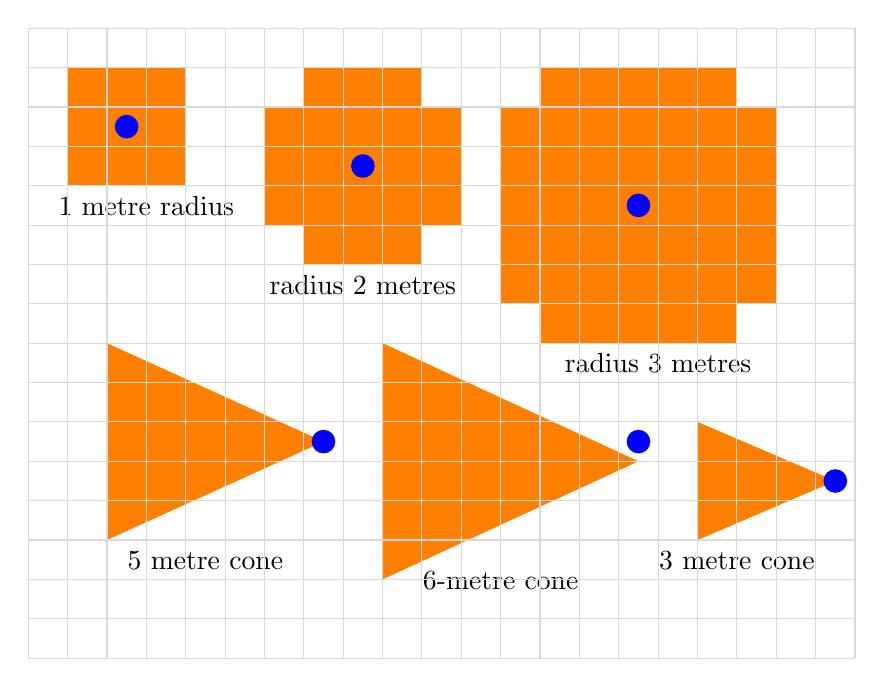
\begin{tikzpicture}[scale=0.5]


\fill[orange] (1,17) rectangle (4,20);
\fill[blue] (2.5,18.5) circle (0.3);
\node at (3,16) [above] {1 metre radius};

\fill[orange] (6,15) rectangle (11,20);
\fill[white] (5,20) rectangle (6,21);
\fill[white] (6,19) rectangle (7,20);
\fill[white] (10,15) rectangle (11,16);
\fill[white] (6,15) rectangle (7,16);
\fill[white] (10,19) rectangle (11,20);
\fill[blue] (8.5,17.5) circle (0.3);
\node at (8.5,14) [above] {radius 2 metres};

\fill[orange] (12,13) rectangle (19,20);
\fill[white] (12,19) rectangle (13,20);
\fill[white] (18,13) rectangle (19,14);
\fill[white] (12,13) rectangle (13,14);
\fill[white] (18,19) rectangle (19,20);
\fill[blue] (15.5,16.5) circle (0.3);
\node at (16,12) [above] {radius 3 metres};


\fill[orange] (2,8) -- (7.5,10.5) -- (2,13) -- cycle;
\fill[blue] (7.5,10.5) circle (0.3);
\node at (4.5,7) [above] {5 metre cone};


\fill[orange] (17,8) -- (20.5,9.5) -- (17,11) -- cycle;
\fill[blue] (20.5,9.5) circle (0.3);
\node at (18,7) [above] {3 metre cone};

%\fill[orange] (9,7) -- (15.5,10.5) -- (9,13) -- cycle;
%\fill[blue] (15.5,10.5) circle (0.3);
%\node at (12,6.5) [above] {6-metre cone};

\fill[orange] (9,7) -- (15.5,10) -- (9,13) -- cycle;
\fill[blue] (15.5,10.5) circle (0.3); % Blue point on the right tip
\node at (12,6.5) [above] {6-metre cone};

% Cube with 3 squares on each side
%\fill[orange] (2.2) -- (5.2) -- (5.5) -- (2.5) -- cycle; % Front face
%\fill[orange] (5.2) -- (6.3) -- (6.6) -- (5.5) -- cycle; % Right face
%\fill[orange] (2.5) -- (5.5) -- (6.6) -- (3.6) -- cycle; % Top face

% Cube with 6 squares on each side
%\fill[orange] (8.2) -- (14.2) -- (14.8) -- (8.8) -- cycle; % Front face
%\fill[orange] (14,2) -- (16,4) -- (16,10) -- (14,8) -- cycle; % Right face
%\fill[orange] (8,8) -- (14,8) -- (16,10) -- (10,10) -- cycle; % Top face

% Draw the base grid (20x15)
\foreach \x in {0,...,20}
\foreach \y in {5,...,20}
\draw[gray!30] (\x,\y) grid (\x+1,\y+1);


\end{tikzpicture}

\medskip

The blue dot determines the origin of the spell

\bigskip

\textbf{Examples of enemy range}

\medskip

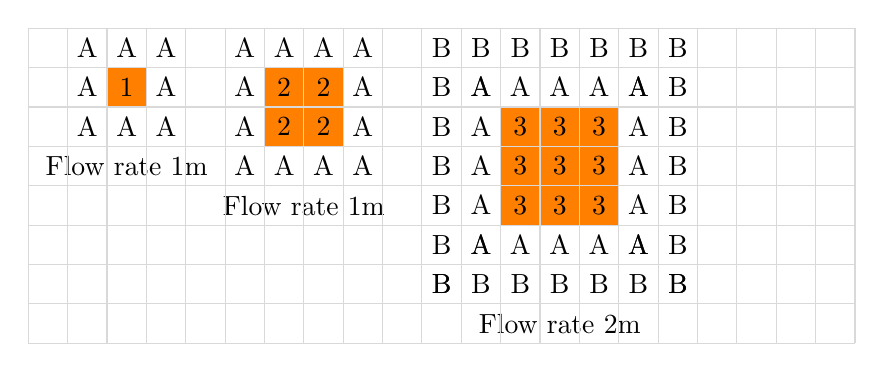
\begin{tikzpicture}[scale=0.5]


\fill[orange] (1,18) rectangle (2,19);
\node at (1.5,18.5) {1};

\foreach \x in {-1,...,1} {
\node at (\x+1.5,17.5) {A};
\node at (\x+1.5,19.5) {A};
}

\foreach \y in {18} { \node at (+0.5,\y+0.5) {A};
\node at (2.5,\y+0.5) {A}; }

\node at (1.5,16) [above] {Flow rate 1m};


% 2x2 central square with the number 2 inside
\fill[orange] (5,17) rectangle (7,19);
\node at (5.5,17.5) {2}; 
\node at (5.5,18.5) {2}; 
\node at (6.5,17.5) {2}; 
\node at (6.5,18.5) {2}; 

% Letters A around the central 2x2 square
\foreach \x in {3,...,6} {
\node at (\x+1.5,19.5) {A}; % Above
\node at (\x+1.5,16.5) {A}; % Below
}
\foreach \y in {9,...,10} {
\node at (4.5,\y+8.5) {A}; % Left
\node at (7.5,\y+8.5) {A}; % Right
}

\node at (6,15) [above] {Flow rate 1m};


% 3x3 square with the number 3 inside, moved 1 square to the left and raised 1 square
\fill[orange] (11,15) rectangle (14,18);
\node at (11.5,17.5) {3}; 
\node at (12.5,17.5) {3}; 
\node at (13.5,17.5) {3}; 

\node at (11.5,16.5) {3}; 
\node at (12.5,16.5) {3}; 
\node at (13.5,16.5) {3}; 

\node at (11.5,15.5) {3};
\node at (12.5,15.5) {3};
\node at (13.5,15.5) {3};

% First frame of squares with the letter A
% Above and below the 3x3 square
\foreach \x in {10,...,14} {
\node at (\x+0.5,14.5) {A};
\node at (\x+0.5,18.5) {A};
}

% On the sides of the 3x3 square
\foreach \y in {13,...,17} {
\node at (10.5,\y+1.5) {A};
\node at (14.5,\y+1.5) {A};
}

% Second frame of squares with the letter B
% Above and below the first frame
\foreach \x in {9,...,15} {
\node at (\x+0.5,19.5) {B};
\node at (\x+0.5,13.5) {B};
}

% On the sides of the first frame
\foreach \y in {13,...,18} {
\node at (9.5,\y+0.5) {B};
\node at (15.5,\y+0.5) {B};
}
\node at (12.5,12) [above] {Flow rate 2m};



\foreach \x in {-1,...,19}
\foreach \y in {12,...,19}
\draw[gray!30] (\x,\y) grid (\x+1,\y+1);

\end{tikzpicture}

\pagebreak


\noindent

\section{Author and Contributions}\index{Author}

\textbf{Author}: Andres Zanzani - azanzani@gmail.com

\medskip

\noindent\textbf{Contributions}: Federica Angeli

\section{Game materials}\index{Card}\index{Manual}\index{Screen}\index{Character information}

\label{card-and-manual}

You are invited to download \textbf{Old Bell School System} from GitHub freely and without restrictions other than those expressed in the licence.
The main website is \href{https://github.com/buzzqw/TUS}{https://github.com/buzzqw/TUS}

\medskip

* \textbf{OBSS Manual}:
\href{https://github.com/buzzqw/TUS/blob/master/OBSS/OBSSv2-eng.pdf}{OBSSv2-eng.pdf}

https://github.com/buzzqw/TUS/blob/master/OBSS/OBSSv2-eng.pdf

\smallskip

* \textbf{Character Sheet}:
\href{https://github.com/buzzqw/TUS/blob/master/OBSS/OBSS-sheet-eng.pdf}{OBSS-sheet-eng.pdf}

https://github.com/buzzqw/TUS/blob/master/OBSS/OBSS-sheet-eng.pdf

\smallskip

%3-page version 
%\href{https://github.com/buzzqw/TUS/blob/master/OBSS/OBSS-scheda-v3.pdf}{OBSS-scheda-v3.pdf}
%https://github.com/buzzqw/TUS/blob/master/OBSS/OBSS-scheda-v3.pdf

\smallskip

* \textbf{Narrator's screen}:
\href{https://github.com/buzzqw/TUS/blob/master/OBSS/screenv2.pdf}{screenv2.pdf}

https://github.com/buzzqw/TUS/blob/master/OBSS/screenv2.pdf

\smallskip

* \textbf{Character info}:
\href{https://github.com/buzzqw/TUS/blob/master/OBSS/OBSS-schema-arbiter-character-eng.pdf}{OBSS-schema-arbiter-character-eng.pdf}

https://github.com/buzzqw/TUS/blob/master/OBSS/OBSS-schema-arbiter-character-eng.pdf

\smallskip

* \textbf{Changelog - only italian} \href{https://github.com/buzzqw/TUS/blob/master/OBSS/changelog.md}{changelog.md}

https://github.com/buzzqw/TUS/blob/master/OBSS/changelog.md

\smallskip

* \textbf{Reports}

For any reports or advice, open an issue on GitHub, or send me an email at azanzani@gmail.com% or contact me on the OBSS group on Telegram \href{https://t.me/obssgdr}{https://t.me/obssgdr}

\section{Acknowledgements}\index{Acknowledgements}\index{DnD SRD}

%To my friends, my fellow adventurers, and all players who close their eyes and let their imagination guide them on fantastic adventures.

Part of the material is adapted from \href{https://media.wizards.com/2023/downloads/dnd/SRD_CC_v5.1_IT.pdf}{SRD\_CC\_v5.1\_IT.pdf} released by Wizard of the Coast.

Link https://media.wizards.com/2023/downloads/dnd/SRD\_CC\_v5.1\_IT.pdf

\medskip

%I would like to thank \href{https://github.com/ThomasJockin/readexpro}{Readex} ( https://github.com/ThomasJockin/readexpro ) for the font used. Readex is a highly legible font, even for people with reading difficulties.

I would like to thank \href{https://www.brailleinstitute.org/freefont/}{Braille Institute} for the font used. Atkinson Hyperlegible Font is a highly legible font, even for people with reading difficulties.

\section{Licence}\hypertarget{Licence}{}\label{Licence}

\textbf{Old Bell School System (OBSS)} © 2021 by Andres Zanzani is licensed under \hyperref{https://creativecommons.org/licenses/by-sa/4.0/legalcode}{}{}{CC BY-SA 4.0} 

The images in the manuals are unlicensed or in the public domain. Images marked with \emph{B.I.C.} and the cover were created with Bing Image Creator. If any copyrighted images are included, please notify us so that we can remove them.

Please contact me before using OBSS or any part of it.

\vspace{0.8cm}

\noindent\begin{minipage}{0.5\textwidth}% adapt widths of minipages to your needs
\includegraphics[keepaspectratio,width=\linewidth]{immagini/CC_BY-SA_icon.svg.png}
\end{minipage}
%
\begin{minipage}{0.5\textwidth}\raggedleft
\large{Powered by} \Huge\LaTeX\ {\normalsize {\&}} \Huge\textbf{GitHub}
\end{minipage}

\vfill

\begin{changemargin}{0.3cm}{0.3cm}\begin{enfasi}{
\begin{center}
And enjoy the game. (Players' Guide to Immortals. Frank Mentzer)
\end{center}
}\end{enfasi}\end{changemargin}

%\vspace{0.5cm}


\thispagestyle{plain}
\begin{center}
\includepdf[pages={1,2},addtotoc={1,section,0,Character Sheet,incl:first},scale=0.9]{OBSS-scheda.pdf}
%\includepdf[pages={1,2},scale=0.85]{OBSS-scheda.pdf}
\end{center}


%\thispagestyle{plain}
%\begin{center}
%\begin{tikzpicture}[remember picture,overlay]
%\node[anchor=south west,inner sep=0pt] at ($(current page.south west)+(1cm,1cm)$) {
%\includegraphics[scale=0.93]{OBSS-scheda-0.png}
%};
%\end{tikzpicture}
%\end{center}
%\pagebreak
%\thispagestyle{plain}
%\begin{center}
%\begin{tikzpicture}[remember picture,overlay]
%\node[anchor=south west,inner sep=0pt] at ($(current page.south west)+(1cm,1cm)$) {
%\includegraphics[scale=0.93]{OBSS-scheda-1.png}
%};
%\end{tikzpicture}
%\end{center}

\pagebreak


\section{My Options}\index{My Options}

\normalsize

I am also a Storyteller, and although I have built OBSS according to my preferences, there are some Options that make the game more \emph{unique} that I like to make available to the characters.

At my gaming table, I usually propose these Options, to be decided in Session Zero:

\begin{itemize}[leftmargin=*] \setlength{\itemsep}{0pt}

\item
\hyperlink{partialsuccess}{Partial Success} page \pageref{partialsuccess}

\item
\hyperlink{initiativevariant}{Initiative Variant}, only if I have experienced players. Page \pageref{initiativevariant}

\item
Starting with \hyperlink{variantetiricritici}{Critical Roll Variant}. \hyperlink{tirocriticovariante}{Critical Roll Variant}, \hyperlink{OptionalCriticalHitActions}{Optional Critical Roll Actions}, \hyperlink{multipleattackvariant}{Multiple Attack Variant} are optional for the player to use. Page \pageref{tirocriticovariante}, page \pageref{OptionalCriticalHitActions}, page \pageref{variantetiricritici} and page \pageref{multipleattackvariant}. These are suggested options for experienced players.  

\item \hyperlink{elencotalentiarmi}{Optional - List of Weapon Manoeuvres} (page \pageref{elencotalentiarmi}) to make fumbling less \emph{noisy}...

%\item
%\hyperlink{lunicaregola}{The Only Rule} I use this if I am the Narrator of a group of beginners. Page \pageref{lunicaregola}

\item 
\hyperlink{Single-Mindedness}{One belief} or \hyperlink{listfeats}{List Feat}, at the player's choice.

\item
\hyperlink{componentsasofferings}{Components as an offering} for a personal, different and unique spell, always linked to the character. Page \pageref{componentsasofferings} 

\item
\hyperlink{iconicfeats}{Iconic Feats} in case of long campaigns. Page \pageref{iconicfeats}

\item
\hyperlink{drugs}{Drugs} \textbf{NO}. Only in case of groups composed of mature and adult players. Page \pageref{drugs}

\item
\textbf{No use of a timer on Lights}: if your adventures are not set in dungeons or you want a more streamlined management, do not manage the duration of lights in real time.

\end{itemize}


\vfill
{\small

\begin{multicols}{2}

\subsubsection*{Notes}

For me, OBSS should be played in a straightforward manner, without too many thoughts or convoluted plans. OBSS is not designed to kill characters, but neither does it facilitate their survival. It is up to the Narrator to decide how to play. The key to the game lies in the Narrator, the style of the players and the interest of the group. OBSS aims to provide the framework and tools to play the adventure.

Try to emphasise the scenes, be theatrical in your descriptions, remove the veneer of clean and politically correct play. It is still your world, your table and your game, so try to create the immersive experience that is often lost in more modern systems.
When there is a fight, make it a fight! You should hear the clang of weapons, the clash of armour, the ozone in the air caused by lightning, the crackling burns of fireballs. Make the players appreciate the possibilities offered by the system and have fun trying to find the best way to check.

You choose whether the characters are scoundrels just trying to survive and accumulate treasure, or whether you want to give the adventure a more classic or epic feel. OBSS lends itself to both choices, especially by using some options over others.

Create the group, and I don't just mean as a set of characters, but also as a group of players. A group where people respect and trust each other (hopefully...). Build adventures that involve everyone, where everyone can contribute. There may be adventures more ‘tailored’ to one character, but this does not have to exclude others from participating, in the broadest sense of the word. Don't let the session be a monologue between you and a single player.
Take advantage of every adventure to get the characters to know each other; nothing unites people more than the fear of dying!

Once you have formed the group, and this may take some time, then use the personal stories, clues and hypotheses created by the players to shape situations and events. Like a heavy spinning top, this will continue to create situations, adventures and new plots to follow.

There may be difficulties in creating the group, unfortunately. Try to talk to the player who is causing problems. Try to understand if it is their character that is not \emph{working} with the group or if it is the player who has not fully understood the mechanics of the group.

For this reason, I always suggest doing the so-called \hyperlink{sessionezero}{Session Zero} (page \pageref{sessionezero}), where, as the Narrator, you will outline the main points of the adventure, what you expect from the characters, and the basic rules and morals to follow. There is nothing worse than a group of unconnected characters where everyone wants to do something different and is not interested in the ‘common goal’.

It is very important to understand what the players like; each person and group wants a certain style of play, and it is right to try to accommodate them. If the group wants political adventures or romantic drama, try to give them satisfaction during the adventure. If, on the other hand, they prefer more combat, then don't skimp on fights, as long as they are consistent with the adventure itself.

Make it clear that you need to work together as a group of players and characters in order to play at your best, have fun and increase your chances of survival. No player should be above the others; only the Narrator has the final say.

Finally, always be fair, for better or for worse. There will be unlucky sessions and others where the dice roll just right, where a brilliant idea will save the group. Don't be a Narrator who saves the characters \textbf{always and in any case}; a little help now and then is fine, especially in the most unfortunate sessions, but respect the characters' choices and the outcome of the dice. Remember that the players have Fate Points they can use, unlike the poor monsters!

Personally, I roll all the dice in front of the players.

The Narrator should not steal the show from the characters, but rather build the environment, the drama and the passions around them. There is nothing more annoying than a Narrator with a desire to be the centre of attention, whether in the role of NPCs or in imposing choices and scenes.

And finally, the obvious: have fun, and make an effort to ensure that the session has that mixture of tension, fun and satisfaction. You are people who want to play, have fun and be together, never forget that.
\end{multicols}}

\pagebreak


\begin{multicols}{4}
{\small\printindex}
\end{multicols}

\TotalBox{OBSSv2}\pagebreak

\begin{multicols}{3}
{\small\printindex[Tables]}
\end{multicols}

\vfill

\TotalBox{Tables}\pagebreak

\begin{multicols}{3}
{\small\printindex[Spells]}
\end{multicols}

%\immediate\write18{./contaspell.sh > contaspell.txt}
%\immediate\openin\myscriptresult=./contaspell.txt
%\read\myscriptresult to \ScriptResult
%\immediate\closein\myscriptresult

\vfill

%Total items in this index \ScriptResult

\TotalBox{Spells}\pagebreak



\begin{multicols}{3}
{\small\printindex[MagicItems]}
\end{multicols}


%{\scriptsize\printindex[MagicItems]}


%\immediate\write18{./contaomagici.sh > contaomagici.txt}
%\immediate\openin\myscriptresult=./contaomagici.txt
%\read\myscriptresult to \ScriptResult
%\immediate\closein\myscriptresult

\vfill

%Total items in this index \ScriptResult

\TotalBox{MagicItems}\pagebreak


\begin{multicols}{3}
{\small\printindex[Feat]}
\end{multicols}

\vfill

\TotalBox{Feat}\pagebreak


\begin{multicols}{3}
{\small\printindex[Monsters]}
\end{multicols}

\vfill

\TotalBox{Monsters}

%Total items in this index \ScriptResult

%\immediate\write18{./contamostri.sh > contamostri.txt}
%\immediate\openin\myscriptresult=./contamostri.txt
%\read\myscriptresult to \ScriptResult
%\immediate\closein\myscriptresult

\end{document}
